\PassOptionsToPackage{citestyle=authoryear,bibstyle=authoryear}{biblatex}
\makeatletter
\def\input@path{{../template/}}
\makeatother
\documentclass[traditional=false,draftmark=false,colors=true,fontsetup=feec-fonts.tex,titlesetup=titles-setup.tex]{AJbook}
\usepackage{ajbook-page-layout}
\usepackage{ajbook-cover}
\usepackage[unicode,bookmarksnumbered]{hyperref}
\usepackage{import-compatibility}
\usepackage{caption}
\captionsetup{hypcap=false}
\usepackage{needspace}
\usepackage[noautomatic]{imakeidx}
\AtBeginDocument{%
  \def\crefpairconjunction{和}%
  \def\crefmiddleconjunction{、}%
  \def\creflastconjunction{和}%
  \def\crefrangeconjunction{至}%
}

\setcounter{tocdepth}{3}
\setcounter{secnumdepth}{3}
\setlength{\emergencystretch}{2em}

\hypersetup{
  pdftitle={不可压缩流问题的有限元方法},
  pdfauthor={Volker John},
  bookmarksopen=true,
  bookmarksnumbered=true,
  unicode=true,
  linktoc=all,
  hyperindex=true
}

\addbibresource{references/references.bib}
\makeindex[title=索引,columns=2,intoc=true]
% The class loads hyperref before imakeidx, so restore linked index pages
% explicitly after imakeidx installs its own index writer.
\makeatletter
\let\codex@originalindex\index
\renewcommand\index[2][]{%
  \if\relax\detokenize{#1}\relax
    \ifstrequal{#2}{超收敛}
      {\codex@originalindex{#2|ImportedSuperconvergencePage}}%
      {\codex@originalindex{#2|hyperpage}}%
  \else
    \codex@originalindex[#1]{#2|hyperpage}%
  \fi}
\newcommand\indexsee[2]{\codex@originalindex{#1|see{#2}}}
\makeatother

% ElegantBook recommends fixed-position captions rather than figure floats.
\NewDocumentEnvironment{elegantfigure}{O{0.9\linewidth}}
  {\par\medskip\begingroup\noindent\centering\begin{minipage}{#1}\centering}
  {\end{minipage}\par\endgroup\medskip}
\NewDocumentEnvironment{eleganttable}{O{\linewidth}}
  {\par\medskip\noindent\begin{minipage}{#1}\centering}
  {\end{minipage}\par\medskip}

\newcommand{\ImportedFrontMatter}{%
  \let\SavedBookContents\tableofcontents
  \let\tableofcontents\relax
  \frontmatter
  \let\tableofcontents\SavedBookContents
}
\ExecuteBibliographyOptions{backref=false,sorting=nyt}
\begin{document}
\hypersetup{pageanchor=false}
\AJBookCover{不可压缩流问题的\\有限元方法}
  {Finite Element Methods for\\Incompressible Flow Problems}
  {Volker John}

\hypersetup{pageanchor=true}
\ImportedFrontMatter
\chapter*{前言}
不可压缩流问题出现在许多物理过程及其应用模型中.对这类问题进行数值模拟,尤其需要作空间离散.有限元方法是数学上研究得最为透彻的一类离散方法.

本书主要讨论不可压缩流问题有限元方法的数学方面,读者对象包括研究人员、博士生,以及有志攻读硕士学位的学生.本书对所讨论的内容,特别是数学论证,作了细致阐述.采用这种写法,是希望帮助读者理解这一主题,尤其是相关经验尚不丰富的读者.

本书的大部分内容曾在柏林自由大学连续三门硕士课程中讲授,本书即以相应的课程讲义为基础.首先,我要感谢参加这些课程的学生,其中不少人后来在我的指导下完成了硕士学位论文.接下来,我要感谢两位合作者:Julia Novo(马德里)和 Gabriel R. Barrenechea(格拉斯哥).他们阅读了本书的部分内容,并提出了宝贵的改进建议.最重要的是,我要感谢我亲爱的妻子 Anja 和女儿 Josephine,她们一直给予我支持与鼓励.在过去三年里,她们承担日常生活中的许多事务,为我腾出写作时间;这对本书的完成作出了不可估量的贡献.

\begin{flushright}
德国 Colbitz\par
2016 年 7 月\par
Volker John
\end{flushright}

\tableofcontents
\mainmatter
\chapter{引言}\label{chap:introduction}

不可压缩流体的运动由不可压缩 Navier--Stokes 方程组(incompressible Navier--Stokes equations)描述\index{buke-yasuo-liu@不可压缩流}.该方程组表达了线动量守恒\index{xian-dongliang@线动量守恒}和质量守恒.在稳态\index{wending@稳态流动}且流体黏度较大的特殊情形下,Navier--Stokes 方程组\index{navier-stokes@纳维--斯托克斯方程组}可以用 Stokes 方程(Stokes equations)\index{stokes@斯托克斯方程}近似.不可压缩流问题不仅本身值得研究,也是许多复杂模型的一部分;这些模型用于描述自然现象以及工程和工业过程.

通常无法求得 Stokes 方程或 Navier--Stokes 方程的解析解(analytical solution)\index{jiexi-jie@解析解},因此必须采用数值方法(numerical methods)来近似其解.为此,需要对方程进行离散(discretization)\index{lisan@离散};一般而言,既要作时间离散(temporal discretization),也要作空间离散(spatial discretization).本书讨论空间离散中的有限元方法(finite element method, FEM)\index{youxianyuan-fangfa@有限元方法}.有限元方法应用广泛,从数学角度看,对它的理解也相当深入.

早在 20 世纪 70 年代,人们就开始使用有限元方法模拟 Stokes 方程和 Navier--Stokes 方程.同一时期,对这两类方程的有限元分析也开始发展.例如,\textcite{Babuska1971} 和 \textcite{Brezzi1974} 引入了 inf-sup 条件(inf-sup condition)\index{inf-sup@inf-sup 条件};这一条件是连续问题和有限元问题适定性(well-posedness)的基础.早期有限元分析成果汇集于 \textcite{GiraultRaviart1979} 的专著中.该书的扩充版 \textcite{GiraultRaviart1986} 成为这一领域的经典参考著作.自其出版以来,三十年间出现了许多新的进展,也取得了大量新成果.较近出版、研究不可压缩流问题有限元方法或其重要方面的专著包括 \textcite{Layton2008}、\textcite{Boffi2008} 和 \textcite{Elman2014}.

本书一方面覆盖范围广泛,从 Navier--Stokes 方程的推导一直延伸到湍流模拟;另一方面,有不少主题若要详细阐述,足以自成一部专著,因此本书只作概述.本书着重讨论数学问题.除了有限元方法的许多结果,本书也详细介绍了连续方程的一些基本结果,因为理解连续问题的分析,是全面理解所研究问题的重要基础.

本书的一项主要特点,是对数学工具和大多数证明作了细致讲解.这种写法源于我过去的体会:有时,为了理解文献中常见的简略证明步骤,会花费(甚至浪费)很多时间.其实,若能多给一点提示,或在估计中再多写一行,许多步骤就很容易理解.因此,本书尽可能做到自成体系,使读者理解其中大多数数学结果时无需另查其他文献.总的来说,本书面向广泛的读者群体:本领域的资深研究人员、青年研究人员和硕士生.硕士生也能有效利用本书这一点,已经在教学实践中得到验证.本书的大部分内容曾在柏林自由大学 2013 至 2015 年间开设的硕士课程中讲授;此后,有多篇硕士论文围绕这些课程涉及的主题完成.

\section{本书内容}\label{sec:contents-of-monograph}
\markright{\thesection\ 本书内容}

第 2 章依据质量守恒和线动量守恒,概述不可压缩 Navier--Stokes 方程的推导.随后从物理考虑出发,推导应力张量的重要性质;介绍无量纲方程,并讨论恰当的边界条件.

本书以下各章的安排,围绕第 2 章指出的不可压缩 Navier--Stokes 方程固有的困难展开:
\begin{itemize}
  \item 首先研究速度与压力之间的耦合:
    \begin{itemize}
      \item 第 3 章介绍抽象理论,并讨论如何选取恰当的有限元空间;
      \item 第 4 章将该抽象理论用于 Stokes 方程.
    \end{itemize}
  \item 其次考虑对流占主导这一问题:第 5 章针对 Oseen 方程研究这一主题.Oseen 方程是一类线性化的 Navier--Stokes 方程.
  \item 最后,在前述两项困难之外进一步考虑 Navier--Stokes 方程的非线性:
    \begin{itemize}
      \item 第 6 章研究低雷诺数下出现的稳态流动;
      \item 第 7 章研究中等雷诺数下出现的层流;
      \item 第 8 章研究高雷诺数下出现的湍流.
    \end{itemize}
\end{itemize}

在不可压缩流问题中,速度与压力的耦合意味着不能直接任意选取有限元空间对.为了使问题适定,这些空间必须满足所谓的离散 inf-sup 条件.第 3 章将推导这一条件.推导以抽象线性鞍点问题的适定性研究为基础.首先把抽象理论用于连续线性不可压缩流问题,由此确定速度和压力所适用的函数空间;这些函数空间满足所谓的 inf-sup 条件.接着,本章讨论:连续 inf-sup 条件成立,并不自动保证离散 inf-sup 条件成立.书中给出了不满足该离散条件的速度与压力有限元空间对的例子,随后介绍若干验证离散 inf-sup 条件的技巧,并给出重要的 inf-sup 稳定有限元空间对.对于其中一些空间对,本章还会证明其满足离散 inf-sup 条件,并介绍如何计算离散 inf-sup 常数.本章最后一节讨论 Helmholtz 分解.

第 4 章把上一章建立的理论用于 Stokes 方程.Stokes 方程是线性方程组,也是最简单的不可压缩流模型,只描述由黏性力引起的流动.本章先讨论弱解的存在性、唯一性和稳定性,继而介绍有限元误差分析的结果.误差分析的第一部分研究协调有限元方法,第二部分研究低阶非协调有限元离散;随后给出有限元方法实现方面的一些说明.接下来,本章简要介绍后验误差估计及其在自适应网格加密中的应用.之后讨论绕开离散 inf-sup 条件的若干方法.这些方法使速度和压力可以采用相同的分片多项式空间,从实践角度看颇具吸引力.本章详细分析其中一种方法——PSPG 方法,并简要讨论其他几种方法.一般而言,有限元方法只能近似满足质量守恒.本章最后综述能够减小质量守恒偏差、甚至保证质量守恒的若干方法.

第 5 章研究 Oseen 方程.它是包含黏性(二阶)、对流(一阶)和反应(零阶)项的线性方程.这类方程出现在求解 Navier--Stokes 方程的多种数值方法中,通常对流项或反应项会压过黏性项.分析中的一个主要问题,是追踪稳定性界和误差界对问题系数的依赖.本章先建立方程解的存在性与唯一性,再研究标准 Galerkin 有限元方法.分析表明,当对流或反应占主导时,稳定性界和误差界会变大,数值研究也支持这一结论.为改善数值解,必须采用稳定化方法.本章详细分析一种基于残量的稳定化方法,即 SUPG/PSPG/grad-div 方法,并简要回顾其他若干稳定化方法.

第 6 章研究不可压缩流问题的第一个非线性模型——稳态 Navier--Stokes 方程.首先考察非线性项,介绍其不同形式并推导若干性质.随后研究稳态 Navier--Stokes 方程连续问题的解.结果表明,只有外力足够小且不随时间变化、黏度足够大时,才可期待解唯一存在.针对这一情形,本章给出有限元误差分析,重点在于估计非线性项;然后讨论求解非线性问题的迭代方法.本章最后介绍对偶加权残量(Dual Weighted Residual, DWR)方法,这是一种针对感兴趣的物理量进行后验误差估计的方法.

第 7 章开始研究含时不可压缩 Navier--Stokes 方程.从有限元离散的角度,本章考虑所谓层流,也就是适用标准 Galerkin 有限元方法的流动.开篇简要介绍含时不可压缩 Navier--Stokes 方程弱解的存在性与唯一性分析,并特别阐明为何在实际相关的三维情形下无法证明唯一性.随后介绍连续时间情形下 Galerkin 有限元方法的误差分析;这里的“连续时间”是指尚未对时间作离散.实际模拟必须离散时间,因此本章接下来介绍若干时间步进格式;这些格式在每个离散时刻都要求求解速度与压力耦合问题,其中重点讨论 \(\theta\)-格式.之后以向后 Euler 格式为例,介绍完全离散方程的有限元误差分析.至此介绍的方法都需要求解鞍点问题,这可能带来较高的计算成本.本章最后介绍投影方法,它可以避开鞍点问题:只需分别求解速度场每个分量和压力对应的标量方程.

第 8 章讨论湍流模拟.湍流并没有严格的数学定义,因此本章先描述通常被视为湍流的流场所具有的特征,并勾勒一种描述湍流的数学思路.湍流包含的尺度往往过小,无法在计算成本可接受的网格上分辨;因此必须用所谓湍流模型刻画这些尺度对可分辨尺度的影响.本章主要介绍那些能够进行数学或数值分析,或其推导基于数学论证的湍流模型.大涡模拟(large eddy simulation, LES)是一种非常流行的湍流建模方法,它通过空间平均,只模拟较大的(可解析)尺度.关于 LES 的第一节推导这些尺度对应的方程,尤其考察其中关于微分运算与空间平均可交换的假设;本章指出,通常会出现不可忽略的交换误差.下一节介绍最流行的 LES 模型——Smagorinsky 模型;针对这一模型,已有较完善的数学和数值分析.之后介绍基于波数空间近似推导的 LES 模型,最后讨论近似解卷积模型(Approximate Deconvolution Models, ADM).接着介绍 Leray--\(\alpha\) 模型,该模型通过正则化速度场构造.随后讨论 Navier--Stokes--\(\alpha\) 模型,其推导基于对拉格朗日泛函及相应轨线的研究.本章还介绍变分多尺度(Variational Multiscale, VMS)方法.与 LES 不同,VMS 方法通过适当函数空间中的投影来定义需要模拟的大尺度.VMS 方法主要分为两类:基于两尺度分解的方法,以及基于三尺度分解的方法.本章详细介绍五种不同的 VMS 方法实现,最后给出若干湍流数值模拟研究,其中使用了 Smagorinsky 模型和一种有代表性的 VMS 模型.

对不可压缩 Navier--Stokes 方程进行线性化和离散后,许多方法会得到速度与压力耦合的代数方程组.第 9 章简要介绍这类方程组的求解器,包括稀疏直接求解器和迭代求解器;后者需要配合恰当的预条件子.本章着重介绍一种耦合多重网格方法,它被用于本书大多数数值算例.

附录 A 汇集泛函分析的一些基本记号、若干不等式和定理;这些结果用于本书的分析和数值分析.附录 B 介绍有限元方法的一些基础知识,特别详细描述用于离散不可压缩流问题的有限元空间.附录 C 讨论如何通过插值或投影逼近 Sobolev 空间中的函数,并给出有限元误差分析中大量使用的相应估计.附录 D 介绍若干数值模拟算例,并将它们分为三组:稳态流问题算例、含时层流问题算例和湍流问题算例.这些算例用于开展本书所呈现的数值模拟.原书目录还列有附录 E“记号”,本中文版将依原书一并收录.

柏林自由大学开设的硕士课程覆盖以下主题:
\begin{itemize}
  \item 课程 1:第 2、3 章,以及第 4 章第 4.1--4.3 节;
  \item 课程 2:第 4 章第 4.4--4.6 节,第 5--7 章,以及第 9 章;
  \item 课程 3:第 8 章.
\end{itemize}
当然,在这些课程中,讲授内容只集中于各主题中最重要的问题.

\chapter{Navier--Stokes 方程组:不可压缩流动的数学模型}\label{chap:navier-stokes}\label{chap:flow-equations}

\begin{note}[基本原理和变量]\label{note:basic-principles}
流体力学的基本方程称为 Navier--Stokes 方程组.对于等温流动(isothermal flow),也就是温度保持恒定的流动,它表达两条物理守恒定律:质量守恒(conservation of mass)和线动量守恒(conservation of linear momentum).推导这些方程有多种方法.这里概述连续介质力学(continuum mechanics)中的经典推导;这种方法包含若干启发式步骤.

流动由以下变量描述:
\begin{itemize}
  \item $\rho(t,\bm{x})$:密度,单位为 $\mathrm{kg}/\mathrm{m}^3$;
  \item $\bm{v}(t,\bm{x})$:速度,单位为 $\mathrm{m}/\mathrm{s}$;
  \item $P(t,\bm{x})$:压力,单位为 $\mathrm{Pa}=\mathrm{N}/\mathrm{m}^2$.
\end{itemize}
假设这些函数在时间区间 $[0,T]$ 和区域 $\Omega\subset\mathbb{R}^3$ 上具有足够的光滑性.
\end{note}

\section{质量守恒}\label{sec:mass-conservation}
\markright{\thesection\ 质量守恒}

\begin{note}[一般守恒律]\label{note:general-conservation-law}
取 $\Omega$ 中任意一个固定不动的开体积区域 $\Omega$,假设其边界 $\partial\Omega$ 足够光滑.区域 $\Omega$ 内的质量为
\begin{equation*}
  m(t)=\int_{\Omega}\rho(t,\bm{x})\,\mathrm{d}\bm{x}\quad[\mathrm{kg}].
\end{equation*}
如果 $\Omega$ 内的质量守恒,那么区域内质量的变化率必须等于穿过 $\Omega$ 边界的质量通量(mass flux).质量通量为 $\rho\bm{v}(t,\bm{x})$,单位是 $\mathrm{kg}/(\mathrm{m}^2\mathrm{s})$,因此
\begin{equation}\label{eq:mass-balance-integral}
  \frac{\mathrm{d}}{\mathrm{d}t}m(t)
  =\frac{\mathrm{d}}{\mathrm{d}t}\int_{\Omega}\rho(t,\bm{x})\,\mathrm{d}\bm{x}
  =-\int_{\partial\Omega}\rho(t,\bm{s})\,\bm{v}(t,\bm{s})\cdot\bm{n}(\bm{s})\,\mathrm{d}s.
\end{equation}
这里 $\bm{n}(\bm{s})$ 是边界上指向外侧的单位法向量.
\end{note}

假设所有函数以及 $\partial\Omega$ 都足够光滑,就可以应用散度定理(divergence theorem,即分部积分公式):
\begin{equation*}
  \int_{\Omega}\nabla\cdot(\rho\bm{v})(t,\bm{x})\,\mathrm{d}\bm{x}
  =\int_{\partial\Omega}(\rho\bm{v})(t,\bm{s})\cdot\bm{n}(\bm{s})\,\mathrm{d}s.
\end{equation*}
将这一恒等式代入\cref{eq:mass-balance-integral},并交换对时间的微分与对空间的积分,得到
\begin{equation*}
  \int_{\Omega}\bigl(\partial_t\rho(t,\bm{x})+
    \nabla\cdot(\rho\bm{v})(t,\bm{x})\bigr)\,\mathrm{d}\bm{x}=0.
\end{equation*}
由于 $\Omega$ 是任意选取的体积区域,必有
\begin{equation}\label{eq:continuity-equation}
  \partial_t\rho+\nabla\cdot(\rho\bm{v})=0,
  \qquad 0<t<T,\quad\bm{x}\in\Omega.
\end{equation}
这就是流体力学的第一条方程,称为连续性方程.

\begin{note}[随时间变化的区域]\label{note:time-dependent-domain}
也可以考虑随时间变化的区域 $\Omega(t)$.此时可以应用 Reynolds 输运定理(Reynolds transport theorem).设 $\eta(t,\bm{x})$ 是定义在任意区域 $\Omega(t)$ 上且足够光滑的函数,区域边界 $\partial\Omega(t)$ 也足够光滑,则 Reynolds 输运定理为
\begin{equation}\label{eq:reynolds-transport}
  \frac{\mathrm{d}}{\mathrm{d}t}\int_{\Omega(t)}\eta(t,\bm{x})\,\mathrm{d}\bm{x}
  =\int_{\Omega(t)}\partial_t\eta(t,\bm{x})\,\mathrm{d}\bm{x}
   +\int_{\partial\Omega(t)}\eta(t,\bm{s})\,\bm{v}(t,\bm{s})\cdot\bm{n}(\bm{s})\,\mathrm{d}s.
\end{equation}
\end{note}

在 $\eta(t,\bm{x})$ 取为密度的特殊情形下,区域内质量的变化率为
\begin{equation*}
  \frac{\mathrm{d}}{\mathrm{d}t}\int_{\Omega(t)}\rho(t,\bm{x})\,\mathrm{d}\bm{x}
  =\int_{\Omega(t)}\partial_t\rho(t,\bm{x})\,\mathrm{d}\bm{x}
   +\int_{\partial\Omega(t)}\rho(t,\bm{s})\,\bm{v}(t,\bm{s})\cdot\bm{n}(\bm{s})\,\mathrm{d}s.
\end{equation*}
由质量守恒和散度定理可得
\begin{equation*}
  0=\int_{\Omega(t)}\bigl(\partial_t\rho+\nabla\cdot(\rho\bm{v})\bigr)(t,\bm{x})\,\mathrm{d}\bm{x}.
\end{equation*}
由于 $\Omega(t)$ 任意,\cref{eq:continuity-equation} 仍然成立.

\begin{note}[不可压缩均质流体]\label{note:incompressible-homogeneous}
如果流体不可压缩且均质,也就是只由一种流体组成,那么 $\rho(t,\bm{x})=\rho>0$ 为常数,\cref{eq:continuity-equation} 化为
\begin{equation}\label{eq:divergence-free}
  \partial_x v_1+\partial_y v_2+\partial_z v_3
  =\nabla\cdot\bm{v}=0,
  \qquad 0<t<T,\quad\bm{x}\in\Omega.
\end{equation}
其中
\begin{equation*}
  \bm{v}(t,\bm{x})=
  \begin{pmatrix}v_1(t,\bm{x})\\v_2(t,\bm{x})\\v_3(t,\bm{x})\end{pmatrix}.
\end{equation*}
因此,对于不可压缩均质流体,质量守恒只对速度施加约束.
\end{note}

\section{线动量守恒}\label{sec:momentum-conservation}
\markright{\thesection\ 线动量守恒}

\begin{note}[牛顿第二运动定律]\label{note:newton-second-law}
线动量守恒是牛顿第二运动定律
\begin{equation}\label{eq:newton-second-law}
  \text{合力}=\text{质量}\times\text{加速度}
\end{equation}
在流动问题中的表达.它指出,一群流体质点的线动量变化率必须等于作用在这群质点上的合力.
\end{note}

\begin{note}[线动量守恒]\label{note:momentum-conservation}
任意区域 $\Omega$ 内的线动量为
\begin{equation*}
  \int_{\Omega}\rho\bm{v}(t,\bm{x})\,\mathrm{d}\bm{x}
  \quad[\mathrm{N}\,\mathrm{s}].
\end{equation*}
因此,可以仿照\cref{note:general-conservation-law},将区域 $\Omega$ 内的线动量守恒写成
\begin{equation*}
  \frac{\mathrm{d}}{\mathrm{d}t}\int_{\Omega}\rho\bm{v}(t,\bm{x})\,\mathrm{d}\bm{x}
  =-\int_{\partial\Omega}\rho\bm{v}(\bm{v}\cdot\bm{n})(t,\bm{s})\,\mathrm{d}s
    +\int_{\Omega}\bm{f}^{\mathrm{net}}(t,\bm{x})\,\mathrm{d}\bm{x}
  \quad[\mathrm{N}],
\end{equation*}
左端表示区域内动量的变化,右端第一项表示动量穿过 $\Omega$ 边界的通量,$\bm{f}^{\mathrm{net}}$ 是区域内的合力密度,单位为 $\mathrm{N}/\mathrm{m}^3$.其中
\begin{equation*}
  \bm{v}(\bm{v}\cdot\bm{n})
  =\begin{pmatrix}
    v_1v_1n_1+v_1v_2n_2+v_1v_3n_3\\
    v_2v_1n_1+v_2v_2n_2+v_2v_3n_3\\
    v_3v_1n_1+v_3v_2n_2+v_3v_3n_3
  \end{pmatrix}
  =\bm{v}\bm{v}^{\top}\bm{n}.
\end{equation*}
应用分部积分,并交换对时间的微分与对区域 $\Omega$ 的积分,可得
\begin{equation*}
  \int_{\Omega}\Bigl(\partial_t(\rho\bm{v})
    +\nabla\cdot(\rho\bm{v}\bm{v}^{\top})\Bigr)(t,\bm{x})\,\mathrm{d}\bm{x}
  =\int_{\Omega}\bm{f}^{\mathrm{net}}(t,\bm{x})\,\mathrm{d}\bm{x}.
\end{equation*}
乘积法则给出
\begin{equation}\label{eq:momentum-product-rule}
\begin{aligned}
  \int_{\Omega}\Bigl(&\partial_t\rho\,\bm{v}+\rho\,\partial_t\bm{v}
      +\bm{v}\bm{v}^{\top}\nabla\rho
      +\rho(\nabla\cdot\bm{v})\bm{v}
      +\rho(\bm{v}\cdot\nabla)\bm{v}\Bigr)(t,\bm{x})\,\mathrm{d}\bm{x}\\
  &=\int_{\Omega}\bm{f}^{\mathrm{net}}(t,\bm{x})\,\mathrm{d}\bm{x}.
\end{aligned}
\end{equation}
在通常的记号 $(\bm{v}\cdot\nabla)\bm{v}$ 中,可以把 $\bm{v}\cdot\nabla$ 理解为算子
\begin{equation*}
  \bm{v}\cdot\nabla=v_1\partial_x+v_2\partial_y+v_3\partial_z,
\end{equation*}
它分别作用于 $\bm{v}$ 的每个分量.文献中也常把 $(\bm{v}\cdot\nabla)\bm{v}$ 写成 $\bm{v}\cdot\nabla\bm{v}$.

对于不可压缩流动,$\rho$ 为常数,且已知 $\nabla\cdot\bm{v}=0$,见\cref{eq:divergence-free};因此,\cref{eq:momentum-product-rule} 化为
\begin{equation*}
  \int_{\Omega}\rho\Bigl(\partial_t\bm{v}
    +(\bm{v}\cdot\nabla)\bm{v}\Bigr)(t,\bm{x})\,\mathrm{d}\bm{x}
  =\int_{\Omega}\bm{f}^{\mathrm{net}}(t,\bm{x})\,\mathrm{d}\bm{x}.
\end{equation*}
由于 $\Omega$ 是任意选取的区域,可得守恒定律
\begin{equation*}
  \rho\Bigl(\partial_t\bm{v}+(\bm{v}\cdot\nabla)\bm{v}\Bigr)
  =\bm{f}^{\mathrm{net}},
  \qquad 0<t<T,\quad\bm{x}\in\Omega.
\end{equation*}
利用\cref{eq:reynolds-transport},也可以对随时间变化的区域 $\Omega(t)$ 推导出同一守恒定律.
\end{note}

\begin{note}[外力]\label{note:external-forces}
作用在 $\Omega$ 上的力包括外力(体力)和内力.外力例如重力、浮力,以及电磁力(在液态金属中).这些力汇总为体力项
\begin{equation*}
  \int_{\Omega}\bm{f}^{\mathrm{ext}}(t,\bm{x})\,\mathrm{d}\bm{x}.
\end{equation*}
\end{note}

\begin{note}[内力、Cauchy 原理与应力张量]\label{note:internal-forces-stress}
内力是流体对自身施加的力,包括压力,以及一个“流体微元”对相邻微元施加的黏性阻力.内力属于接触力,也就是说,它们作用在流体微元 $\Omega$ 的表面上.令 $\bm{t}\,[\mathrm{N}/\mathrm{m}^2]$ 表示这种内力向量,它称为 Cauchy 应力向量(Cauchy stress vector)或牵引向量(traction vector),则作用在 $\Omega$ 上的内力为
\begin{equation*}
  \int_{\partial\Omega}\bm{t}(t,\bm{s})\,\mathrm{d}s.
\end{equation*}
于是,对任意固定不随时间变化的区域 $\Omega$,线动量守恒方程为
\begin{equation}\label{eq:momentum-balance-with-tractions}
\begin{aligned}
  \int_{\Omega}\rho(t,\bm{x})
    \Bigl(\partial_t\bm{v}+(\bm{v}\cdot\nabla)\bm{v}\Bigr)(t,\bm{x})\,\mathrm{d}\bm{x}
  ={}&\int_{\Omega}\bm{f}^{\mathrm{ext}}(t,\bm{x})\,\mathrm{d}\bm{x}\\
    &+\int_{\partial\Omega}\bm{t}(t,\bm{s})\,\mathrm{d}s.
\end{aligned}
\end{equation}

\cref{eq:momentum-balance-with-tractions} 右端表示作用于区域 $\Omega$ 内部及其边界的合力.接下来需要详细描述其中的内力,也就是 $\bm{t}(t,\bm{s})$ 所表示的力.

连续介质力学以 Cauchy 应力原理为基础.Cauchy 对内接触力的设想是:在 $\partial\Omega$ 上任意一个(假想的)平面,都存在一个力;从几何角度看,该力只依赖于平面的取向.因此,$\bm{t}=\bm{t}(\bm{n})$,其中 $\bm{n}$ 是该假想平面指向外侧的单位法向量.

下面说明 $\bm{t}$ 关于 $\bm{n}$ 呈线性依赖.为此,考虑一个四面体区域 $\Omega$,其顶点为
\begin{equation*}
\begin{aligned}
  \bm{p}_0&=(0,0,0)^{\top},\qquad
  \bm{p}_1=(x_1,0,0)^{\top},\\
  \bm{p}_2&=(0,y_2,0)^{\top},\qquad
  \bm{p}_3=(0,0,z_3)^{\top},\\
  &x_1,y_2,z_3>0.
\end{aligned}
\end{equation*}
见\cref{fig:tetrahedron}.包含 $\bm{p}_1,\bm{p}_2,\bm{p}_3$ 的平面记作 $\partial\Omega_{(\bm{n})}$.其指向外侧的单位法向量为
\begin{equation}\label{eq:tetrahedron-normal}
\begin{aligned}
  \bm{n}
  &=\frac{(\bm{p}_2-\bm{p}_1)\times(\bm{p}_3-\bm{p}_1)}
        {\lVert(\bm{p}_2-\bm{p}_1)\times(\bm{p}_3-\bm{p}_1)\rVert_2}\\
  &=\frac{1}{\lVert(\bm{p}_2-\bm{p}_1)\times(\bm{p}_3-\bm{p}_1)\rVert_2}
      \begin{pmatrix}y_2z_3\\z_3x_1\\x_1y_2\end{pmatrix}
   =\begin{pmatrix}n_1\\n_2\\n_3\end{pmatrix}.
\end{aligned}
\end{equation}
法向量为 $-\bm{e}_i$ 的四面体面记作 $\partial\Omega_{(\bm{e}_i)}$,其中 $i=1,2,3$.令 $\bm{t}(\bm{n})$ 表示作用在 $\partial\Omega_{(\bm{n})}$ 上的 Cauchy 应力向量.假设 Cauchy 应力向量只依赖相应表面的法向量,那么它在四面体的每个面上都是常向量,各面的积分便可直接计算.

\begin{elegantfigure}[0.514\paperwidth]
  
\includegraphics[page=23,pagebox=cropbox,trim=106.50bp 97.40bp 107.36bp 356.25bp,clip,width=\linewidth]{../input/source/Finite Element Methods for Incompressible Flow Problems.pdf}
  \captionof{figure}{用于讨论 Cauchy 应力向量关于法向量线性依赖关系的四面体示意图.}\label{fig:tetrahedron}
\end{elegantfigure}

\cref{eq:newton-second-law} 和四面体体积公式给出
\begin{equation}\label{eq:traction-force-balance}
  \bm{t}(\bm{n})\,|\partial\Omega_{(\bm{n})}|
  -\sum_{i=1}^{3}\bm{t}(\bm{e}_i)\,|\partial\Omega_{(\bm{e}_i)}|
  =-\frac{h(\bm{n})}{3}\,|\partial\Omega_{(\bm{n})}|\,\bm{a},
  \qquad[\mathrm{N}],
\end{equation}
其中 $|\cdot|$ 表示相应面的面积,$\bm{t}(\bm{e}_i)$ 是面 $\partial\Omega_{(\bm{e}_i)}$ 上的常应力向量,$\bm{a}$ 是加速度,单位为 $\mathrm{m}/\mathrm{s}^2$;$h(\bm{n})$ 表示面 $\partial\Omega_{(\bm{n})}$ 到原点的距离.利用叉积可计算 $\partial\Omega_{(\bm{n})}$ 的面积:
\begin{equation*}
  |\partial\Omega_{(\bm{n})}|
  =\frac{1}{2}\bigl|(\bm{p}_2-\bm{p}_1)\times(\bm{p}_3-\bm{p}_1)\bigr|_2
  =\frac{1}{2}\left|\begin{pmatrix}y_2z_3\\z_3x_1\\x_1y_2\end{pmatrix}\right|_2.
\end{equation*}
利用\cref{eq:tetrahedron-normal} 对法向量的表示,可以得到
\begin{equation*}
  |\partial\Omega_{(\bm{e}_1)}|
  =\frac{1}{2}y_2z_3
  =\frac{1}{2}n_1\bigl|(\bm{p}_2-\bm{p}_1)\times(\bm{p}_3-\bm{p}_1)\bigr|_2
  =|\partial\Omega_{(\bm{n})}|\,n_1.
\end{equation*}
对 $|\partial\Omega_{(\bm{e}_2)}|$ 和 $|\partial\Omega_{(\bm{e}_3)}|$ 也可得到类似公式.将这些公式代入\cref{eq:traction-force-balance},可得
\begin{equation}\label{eq:traction-normal-limit}
  \bm{t}(\bm{n})-\sum_{i=1}^{3}\bm{t}(\bm{e}_i)n_i
  =-\frac{h(\bm{n})}{3}\,\bm{a}.
\end{equation}
现在令四面体收缩至原点,同时令 $\partial\Omega_{(\bm{n})}$ 沿 $\bm{n}$ 的方向移动.此时\cref{eq:traction-normal-limit} 左端保持不变,而由于 $h(\bm{n})\to0$,右端趋于零.因此,取极限可得
\begin{equation*}
  \bm{t}(\bm{n})
  =\sum_{i=1}^{3}\bm{t}(\bm{e}_i)n_i
  =\begin{pmatrix}\bm{t}(\bm{e}_1)&\bm{t}(\bm{e}_2)&\bm{t}(\bm{e}_3)\end{pmatrix}\bm{n}.
\end{equation*}
这里最后一个矩阵的各列分别为对应的向量.这个关系表明,$\bm{t}(\bm{n})$ 关于 $\bm{n}$ 线性依赖.

因此,Cauchy 应力向量的模型为
\begin{equation}\label{eq:cauchy-stress-model}
  \bm{t}=\bm{S}\bm{n},
\end{equation}
其中 $\bm{S}(t,\bm{x})\,[\mathrm{N}/\mathrm{m}^2]$ 是一个 $3\times3$ 张量,称为应力张量(stress tensor).应力张量表示流动中的全部内力.将\cref{eq:cauchy-stress-model} 代入\cref{eq:momentum-balance-with-tractions} 中表示内力的边界积分,并应用散度定理,得到
\begin{equation*}
  \int_{\partial\Omega}\bm{t}(t,\bm{s})\,\mathrm{d}s
  =\int_{\Omega}\nabla\cdot\bm{S}(t,\bm{x})\,\mathrm{d}\bm{x},
\end{equation*}
这里张量散度按行定义:
\begin{equation*}
  \nabla\cdot\bm{A}
  =\begin{pmatrix}
    \partial_x a_{11}+\partial_y a_{12}+\partial_z a_{13}\\
    \partial_x a_{21}+\partial_y a_{22}+\partial_z a_{23}\\
    \partial_x a_{31}+\partial_y a_{32}+\partial_z a_{33}
  \end{pmatrix}.
\end{equation*}
由于\cref{eq:momentum-balance-with-tractions} 对任意区域 $\Omega$ 都成立,因而
\begin{equation}\label{eq:momentum-equation}
  \rho\Bigl(\partial_t\bm{v}+(\bm{v}\cdot\nabla)\bm{v}\Bigr)
  =\nabla\cdot\bm{S}+\bm{f}^{\mathrm{ext}},
  \qquad 0<t<T,\quad\bm{x}\in\Omega.
\end{equation}
这就是动量方程.
\end{note}

\begin{note}[应力张量的对称性]\label{note:stress-symmetry}
取边界 $\partial\Omega$ 足够光滑的任意区域 $\Omega$,并令合力由\cref{eq:momentum-balance-with-tractions} 右端给出.关于坐标原点 $\bm{0}$ 的力矩(torque)定义为
\begin{equation}\label{eq:torque}
  \bm{M}_0
  =\int_{\Omega}\bm{r}\times\bm{f}^{\mathrm{ext}}\,\mathrm{d}\bm{x}
   +\int_{\partial\Omega}\bm{r}\times(\bm{S}\bm{n})\,\mathrm{d}s
  \quad[\mathrm{N}\,\mathrm{m}],
\end{equation}
这里使用了\cref{eq:cauchy-stress-model},且 $\bm{r}=x\bm{e}_1+y\bm{e}_2+z\bm{e}_3$ 是从原点指向点 $\bm{x}\in\Omega$ 的向量.直接计算可得
\begin{equation*}
  \bm{r}\times(\bm{S}\bm{n})
  =\bigl(\bm{r}\times\bm{S}_{*1}\quad
         \bm{r}\times\bm{S}_{*2}\quad
         \bm{r}\times\bm{S}_{*3}\bigr)\bm{n},
\end{equation*}
其中 $\bm{S}_{*i}$ 表示 $\bm{S}$ 的第 $i$ 列.将此式代入\cref{eq:torque},应用分部积分并使用乘积法则,得到
\begin{equation}\label{eq:torque-volume-form}
\begin{aligned}
  \bm{M}_0
  ={}&\int_{\Omega}\bm{r}\times\bm{f}^{\mathrm{ext}}\,\mathrm{d}\bm{x}
    +\int_{\Omega}\bm{r}\times(\nabla\cdot\bm{S})\,\mathrm{d}\bm{x}\\
   &+\int_{\Omega}\bigl(\partial_x\bm{r}\times\bm{S}_{*1}
       +\partial_y\bm{r}\times\bm{S}_{*2}
       +\partial_z\bm{r}\times\bm{S}_{*3}\bigr)\,\mathrm{d}\bm{x}.
\end{aligned}
\end{equation}
现在考虑处于平衡状态的流体,即作用在流体上的合力为零.于是,\cref{eq:momentum-equation} 右端为零,\cref{eq:torque-volume-form} 的前两个积分之和也为零.此外,平衡还要求 $\bm{M}_0=\bm{0}$.因此,\cref{eq:torque-volume-form} 给出
\begin{equation}\label{eq:stress-symmetry-derivatives}
  \bm{0}=\int_{\Omega}\bigl(\partial_x\bm{r}\times\bm{S}_{*1}
       +\partial_y\bm{r}\times\bm{S}_{*2}
       +\partial_z\bm{r}\times\bm{S}_{*3}\bigr)\,\mathrm{d}\bm{x}.
\end{equation}
由
\begin{equation*}
  \partial_x\bm{r}
  =\lim_{\Delta x\to0}
    \frac{(x+\Delta x)\bm{e}_1-x\bm{e}_1}{\Delta x}
  =\bm{e}_1,
\end{equation*}
以及 $\partial_y\bm{r}=\bm{e}_2$、$\partial_z\bm{r}=\bm{e}_3$,将这些等式代入\cref{eq:stress-symmetry-derivatives},最终得到
\begin{equation*}
  \bm{0}=\int_{\Omega}
  \begin{pmatrix}
    S_{32}-S_{23}\\S_{13}-S_{31}\\S_{21}-S_{12}
  \end{pmatrix}(t,\bm{x})\,\mathrm{d}\bm{x}.
\end{equation*}
该式对任意区域 $\Omega$ 都成立,因此应力张量必为对称张量,即 $\bm{S}=\bm{S}^{\top}$,且只有六个未知分量.
\end{note}

\begin{note}[应力张量的分解]\label{note:stress-decomposition}
为了用\cref{note:basic-principles} 中引入的基本变量建立应力张量模型,将它分解为
\begin{equation}\label{eq:stress-decomposition}
  \bm{S}=\bm{V}-P\bm{I}.
\end{equation}
这里 $\bm{V}\,[\mathrm{N}/\mathrm{m}^2]$ 是黏性应力张量(viscous stress tensor),表示由粒子间摩擦产生的力;$P\,[\mathrm{Pa}]$ 是压力,描述作用在每个流体体积 $\Omega$ 表面上的力;$\bm{I}$ 为单位张量.黏性应力张量将用速度来建模,见\cref{note:viscous-stress}.
\end{note}

\begin{note}[压力]\label{note:pressure}
压力 $P$ 作用于流体体积 $\Omega$ 的表面时,方向总是垂直于表面并指向 $\Omega$ 内部.\cref{eq:stress-decomposition} 中的负号正体现了这一性质,因为
\begin{equation*}
  -\int_{\partial\Omega}P\bm{n}\,\mathrm{d}s
  =-\int_{\Omega}\nabla P\,\mathrm{d}\bm{x}
  =-\int_{\Omega}\nabla\cdot(P\bm{I})\,\mathrm{d}\bm{x}.
\end{equation*}
\end{note}

\begin{note}[黏性应力张量]\label{note:viscous-stress}
只有流体粒子以不同速度运动时,粒子之间才会产生摩擦.因此,黏性应力张量建模为速度梯度的函数.为保证对称性(见\cref{note:stress-symmetry}),它取决于速度梯度的对称部分,即速度形变率张量(velocity rate-of-deformation tensor),简称速度形变张量:
\begin{equation*}
  \bm{D}(\bm{v})
  =\frac{\nabla\bm{v}+(\nabla\bm{v})^{\top}}{2}
  \quad[1/\mathrm{s}].
\end{equation*}
速度梯度是一个张量,其分量为
\begin{equation*}
  (\nabla\bm{v})_{ij}=\partial_jv_i
  =\frac{\partial v_i}{\partial x_j},
  \qquad i,j=1,2,3.
\end{equation*}

如果速度梯度不太大,可以假设这种依赖关系首先是线性的,其次可以忽略高阶导数.对于速度为常数的流动,速度梯度为零,也不会产生摩擦;因此,模型中不应出现速度一阶导数以外的低阶项.满足上述全部条件的张量最一般形式为
\begin{equation*}
  \bm{V}=a\bm{D}(\bm{v})+b(\nabla\cdot\bm{v})\bm{I},
\end{equation*}
其中 $a$ 和 $b$ 不依赖于速度.引入一阶黏度 $\mu\,[\mathrm{kg}/(\mathrm{m}\,\mathrm{s})]$ 和二阶黏度 $\zeta\,[\mathrm{kg}/(\mathrm{m}\,\mathrm{s})]$ 后,流体力学中将该张量写为
\begin{equation}\label{eq:viscous-stress-law}
  \bm{V}=2\mu\bm{D}(\bm{v})
    +\left(\zeta-\frac{2\mu}{3}\right)
      (\nabla\cdot\bm{v})\bm{I}
  \quad[\mathrm{N}/\mathrm{m}^2].
\end{equation}
黏度 $\mu$ 也称为动力黏度(dynamic viscosity)或剪切黏度(shear viscosity).对于流体,\cref{eq:viscous-stress-law} 与固体的 Hooke 定律相对应.
\end{note}

\begin{example}[稳态旋转]\label{ex:steady-rotation}
流体作稳态旋转时,不存在黏性应力,即 $\bm{V}=\bm{0}$.此时速度为
\begin{equation*}
  \bm{v}=\symbf{\Omega}\times\bm{x}
  =\begin{pmatrix}\Omega_1\\\Omega_2\\\Omega_3\end{pmatrix}
   \times\begin{pmatrix}x\\y\\z\end{pmatrix}
  =\begin{pmatrix}
    \Omega_3y-\Omega_2z\\
    \Omega_1z-\Omega_3x\\
    \Omega_2x-\Omega_1y
  \end{pmatrix},
\end{equation*}
其中 $\symbf{\Omega}\,[1/\mathrm{s}]$ 为常角速度(angular velocity).显然,$\nabla\cdot\bm{v}=0$,并且
\begin{equation*}
  \nabla\bm{v}=
  \begin{pmatrix}
    0&\Omega_3&-\Omega_2\\
    -\Omega_3&0&\Omega_1\\
    \Omega_2&-\Omega_1&0
  \end{pmatrix}
  \quad\Longrightarrow\quad
  \bm{D}(\bm{v})=\bm{0}.
\end{equation*}
因此,\cref{eq:viscous-stress-law} 在这种情形下是合适的模型.
\end{example}

\begin{note}[Newton 型流体]\label{note:newtonian-fluid}
线性关系\cref{eq:viscous-stress-law} 只是对真实流体的一种近似.一般而言,这种关系是非线性的;只有在应力较小时,才能对一般的应力--形变关系作线性近似.线性应力--形变关系由 Newton 提出,因此满足\cref{eq:viscous-stress-law} 假设的流体称为 Newton 型流体(Newtonian fluid).还存在比\cref{eq:viscous-stress-law} 更一般的关系,不过从数学角度看,对它们的理解还不够充分.
\end{note}

\begin{note}[法向应力、剪切应力与应力张量的迹]\label{note:stress-trace}
应力张量 $\bm{S}$ 的对角分量 $S_{11},S_{22},S_{33}$ 称为法向应力,非对角分量称为剪切应力.对于不可压缩流动,由\cref{eq:divergence-free,eq:stress-decomposition,eq:viscous-stress-law} 可得
\begin{equation}\label{eq:incompressible-stress}
  \bm{S}=2\mu\bm{D}(\bm{v})-P\bm{I}.
\end{equation}
应力张量的迹是法向应力之和:
\begin{equation*}
\begin{aligned}
  \operatorname{tr}(\bm{S})
  &=S_{11}+S_{22}+S_{33}\\
  &=2\mu(\partial_xv_1+\partial_yv_2+\partial_zv_3)
    +3\left(\zeta-\frac{2\mu}{3}\right)(\nabla\cdot\bm{v})-3P\\
  &=3\zeta(\nabla\cdot\bm{v})-3P.
\end{aligned}
\end{equation*}
对于不可压缩流体,因而有
\begin{equation*}
  \operatorname{tr}(\bm{D}(\bm{v}))
  =\frac{1}{2\mu}\bigl(\operatorname{tr}(\bm{S})
       +\operatorname{tr}(P\bm{I})\bigr)
  =\frac{1}{2\mu}(-3P+3P)=0,
\end{equation*}
并且
\begin{equation}\label{eq:pressure-from-stress-trace}
  P(t,\bm{x})=-\frac{1}{3}
    (S_{11}+S_{22}+S_{33})(t,\bm{x}).
\end{equation}
\end{note}

\begin{note}[Navier--Stokes 方程组]\label{note:full-navier-stokes}
现在将应力张量中的压力部分和黏性应力张量模型\cref{eq:viscous-stress-law} 代入\cref{eq:momentum-equation},得到包含质量守恒方程在内的一般 Navier--Stokes 方程组:
\begin{equation}\label{eq:general-navier-stokes}
\begin{aligned}
  &\rho\bigl(\partial_t\bm{v}
        +(\bm{v}\cdot\nabla)\bm{v}\bigr)
   -2\nabla\cdot\bigl(\mu\bm{D}(\bm{v})\bigr)\\
  &\quad-\nabla\cdot\left(
      \left(\zeta-\frac{2\mu}{3}\right)
      (\nabla\cdot\bm{v})\bm{I}\right)
      +\nabla P=\bm{f}^{\mathrm{ext}},\\
  &\partial_t\rho+\nabla\cdot(\rho\bm{v})=0,
  \qquad (t,\bm{x})\in(0,T)\times\Omega.
\end{aligned}
\end{equation}
如果流体不可压缩且均质,使得 $\mu$ 和 $\rho$ 为正的常数,Navier--Stokes 方程组可简化为
\begin{equation}\label{eq:incompressible-navier-stokes}
\begin{aligned}
  \partial_t\bm{v}-2\nu\nabla\cdot\bm{D}(\bm{v})
    +(\bm{v}\cdot\nabla)\bm{v}
    +\nabla\frac{P}{\rho}
  &=\frac{\bm{f}^{\mathrm{ext}}}{\rho},
  &&(t,\bm{x})\in(0,T)\times\Omega,\\
  \nabla\cdot\bm{v}&=0,
  &&(t,\bm{x})\in(0,T)\times\Omega.
\end{aligned}
\end{equation}
这里 $\nu=\mu/\rho\,[\mathrm{m}^2/\mathrm{s}]$ 是流体的运动黏度(kinematic viscosity).
\end{note}

\section{无量纲 Navier--Stokes 方程组}\label{sec:dimensionless-navier-stokes}
\markright{\thesection\ 无量纲方程}
\markright{\thesection}

\begin{note}[特征尺度]\label{note:characteristic-scales}
数学分析和数值模拟以无量纲方程(dimensionless equations)为基础.为了从\cref{eq:incompressible-navier-stokes} 导出无量纲方程,引入以下量:
\begin{itemize}
  \item $L\,[\mathrm{m}]$:流动问题的特征长度尺度(characteristic length scale);
  \item $U\,[\mathrm{m}/\mathrm{s}]$:流动问题的特征速度尺度(characteristic velocity scale);
  \item $T^*\,[\mathrm{s}]$:流动问题的特征时间尺度(characteristic time scale).
\end{itemize}
\end{note}

\begin{note}[无量纲 Navier--Stokes 方程组]\label{note:dimensionless-equations}
用 $(t',\bm{x}')\,[\mathrm{s},\mathrm{m}]$ 表示原变量.作变量变换
\begin{equation}\label{eq:dimensionless-variable-transform}
  \bm{x}=\frac{\bm{x}'}{L},\qquad
  \bm{u}=\frac{\bm{v}}{U},\qquad
  t=\frac{t'}{T^*}.
\end{equation}
由\cref{eq:incompressible-navier-stokes} 并经尺度变换,得到
\begin{equation*}
\begin{aligned}
  \frac{L}{UT^*}\partial_t\bm{u}
   -\frac{2\nu}{UL}\nabla\cdot\bm{D}(\bm{u})
   +(\bm{u}\cdot\nabla)\bm{u}
   +\nabla\frac{P}{\rho U^2}
  &=\frac{L}{\rho U^2}\bm{f}^{\mathrm{ext}},\\
  \nabla\cdot\bm{u}&=0.
\end{aligned}
\end{equation*}
这里所有导数都针对新变量.虽然记号中没有特别标出,区域和时间区间此时也都已无量纲化.定义
\begin{equation}\label{eq:dimensionless-parameters}
  p=\frac{P}{\rho U^2},\qquad
  \mathrm{Re}=\frac{UL}{\nu},\qquad
  \mathrm{St}=\frac{L}{UT^*},\qquad
  \bm{f}=\frac{L}{\rho U^2}\bm{f}^{\mathrm{ext}}.
\end{equation}
于是得到无量纲形式的不可压缩 Navier--Stokes 方程组:
\begin{equation}\label{eq:dimensionless-navier-stokes}
\begin{aligned}
  \mathrm{St}\,\partial_t\bm{u}
   -\frac{2}{\mathrm{Re}}\nabla\cdot\bm{D}(\bm{u})
   +(\bm{u}\cdot\nabla)\bm{u}+\nabla p
  &=\bm{f},
  &&(t,\bm{x})\in(0,T)\times\Omega,\\
  \nabla\cdot\bm{u}&=0,
  &&(t,\bm{x})\in(0,T)\times\Omega.
\end{aligned}
\end{equation}
常数 $\mathrm{Re}$ 称为 Reynolds 数(Reynolds number),常数 $\mathrm{St}$ 称为 Strouhal 数(Strouhal number).这两个数可用于对不同流动进行分类和比较.
\end{note}

\begin{note}[无量纲 Navier--Stokes 方程组的固有困难]\label{note:dimensionless-difficulties}
为了简化记号,取特征时间 $T^*=L/U$,于是\cref{eq:dimensionless-navier-stokes} 化为
\begin{equation}\label{eq:dimensionless-ns-standard}
\begin{aligned}
  \partial_t\bm{u}-2\nu\nabla\cdot\bm{D}(\bm{u})
    +(\bm{u}\cdot\nabla)\bm{u}+\nabla p
  &=\bm{f},
  &&(t,\bm{x})\in(0,T)\times\Omega,\\
  \nabla\cdot\bm{u}&=0,
  &&(t,\bm{x})\in(0,T)\times\Omega.
\end{aligned}
\end{equation}
这里无量纲黏度(dimensionless viscosity)$\nu=\mathrm{Re}^{-1}$.稍有滥用记号之处在于,此处沿用运动黏度的符号表示无量纲黏度.

上述变换以及由此得到的\cref{eq:dimensionless-ns-standard},是不可压缩 Navier--Stokes 方程数学分析和不可压缩流动数值模拟的基本方程.系统\cref{eq:dimensionless-ns-standard} 包含两个重要困难:
\begin{itemize}
  \item 速度与压力之间的耦合;
  \item 对流项的非线性.
\end{itemize}
此外,当对流项占主导、也就是 $\nu$ 很小时,数值模拟也会遇到困难.
\end{note}

\begin{note}[式 \texorpdfstring{(2.25)}{(2.25)} 中各项的不同形式]\label{note:equivalent-term-forms}
借助散度约束,即\cref{eq:dimensionless-ns-standard} 的第二个方程,可以对 Navier--Stokes 方程组中的黏性项和对流项作等价改写.

设 $\bm{u}$ 足够光滑且 $\nabla\cdot\bm{u}=0$.利用 Schwarz 定理(Schwarz theorem)和\cref{eq:dimensionless-ns-standard} 的第二个方程,直接计算可得
\begin{equation}\label{eq:viscous-laplacian-identity}
\begin{aligned}
  \nabla\cdot(\nabla\bm{u})&=\Delta\bm{u},\\
  \nabla\cdot\bigl((\nabla\bm{u})^{\top}\bigr)
  &=\nabla(\nabla\cdot\bm{u})
   =\begin{pmatrix}
     \partial_x(\nabla\cdot\bm{u})\\
     \partial_y(\nabla\cdot\bm{u})\\
     \partial_z(\nabla\cdot\bm{u})
    \end{pmatrix}
   =\bm{0}.
\end{aligned}
\end{equation}
因此,黏性项可以写成
\begin{equation}\label{eq:viscous-term-laplacian}
  -2\nu\nabla\cdot\bm{D}(\bm{u})=-\nu\Delta\bm{u}.
\end{equation}

对于对流项,利用下列恒等式(乘积法则):
{\small
\begin{equation}\label{eq:convective-product-rule}
\begin{aligned}
  \nabla\cdot(\bm{u}\bm{v}^{\top})
  & =\begin{pmatrix}
      \partial_x(u_1v_1)+\partial_y(u_1v_2)+\partial_z(u_1v_3)\\
      \partial_x(u_2v_1)+\partial_y(u_2v_2)+\partial_z(u_2v_3)\\
      \partial_x(u_3v_1)+\partial_y(u_3v_2)+\partial_z(u_3v_3)
     \end{pmatrix}\\
  & =\begin{pmatrix}
      u_1(\partial_xv_1+\partial_yv_2+\partial_zv_3)\\
      u_2(\partial_xv_1+\partial_yv_2+\partial_zv_3)\\
      u_3(\partial_xv_1+\partial_yv_2+\partial_zv_3)
     \end{pmatrix}
     +\begin{pmatrix}
       v_1\partial_xu_1+v_2\partial_yu_1+v_3\partial_zu_1\\
       v_1\partial_xu_2+v_2\partial_yu_2+v_3\partial_zu_2\\
       v_1\partial_xu_3+v_2\partial_yu_3+v_3\partial_zu_3
      \end{pmatrix}\\
  &=(\nabla\cdot\bm{v})\bm{u}
    +(\bm{v}\cdot\nabla)\bm{u}.
\end{aligned}
\end{equation}
}
在 $\bm{v}=\bm{u}$ 且 $\nabla\cdot\bm{u}=0$ 时,得到
\begin{equation}\label{eq:convective-divergence-form}
  (\bm{u}\cdot\nabla)\bm{u}
  =\nabla\cdot(\bm{u}\bm{u}^{\top}).
\end{equation}
关于对流项不同形式的详细介绍和讨论见第 6.1.2 节.
\end{note}

\begin{note}[二维 Navier--Stokes 方程组]\label{note:two-dimensional-ns}
虽然真实流动只发生在三维空间中,研究二维的 Navier--Stokes 方程组\cref{eq:dimensionless-ns-standard} 也很有意义.有些应用中,流动沿第三个方向保持不变,因而呈现出近似二维的行为.
\end{note}

\begin{note}[不可压缩流动模型的特殊情形]\label{note:special-incompressible-models}
\begin{itemize}
  \item 在稳态流动中,速度和压力不随时间变化,因而 $\partial_t\bm{u}=\bm{0}$.此类流动由所谓稳态或定常 Navier--Stokes 方程组描述:
  \begin{equation}\label{eq:steady-navier-stokes}
  \begin{aligned}
    -\nu\Delta\bm{u}+(\bm{u}\cdot\nabla)\bm{u}
      +\nabla p&=\bm{f},&&\bm{x}\in\Omega,\\
    \nabla\cdot\bm{u}&=0,&&\bm{x}\in\Omega.
  \end{aligned}
  \end{equation}
  流场不随时间变化的必要条件是问题数据(即右端项和边界条件,见第 2.4 节)不随时间变化;但这一条件并不充分,例如附录 D 的例题 8.
  \item 如果稳态流动中黏性输运占主导,即流体运动极为缓慢,则可忽略\cref{eq:steady-navier-stokes} 中 Navier--Stokes 方程组的非线性对流项.由此得到线性方程组,即所谓 Stokes 方程:
  \begin{equation}\label{eq:stokes-equations}
  \begin{aligned}
    -\Delta\bm{u}+\nabla p&=\bm{f},&&\bm{x}\in\Omega,\\
    \nabla\cdot\bm{u}&=0,&&\bm{x}\in\Omega.
  \end{aligned}
  \end{equation}
  这里将动量方程除以 $\nu$,并相应地重新定义了压力和右端项.
  \item 在一些标准的 Navier--Stokes 方程数值求解格式中,会出现所谓 Oseen 方程.给定一个无散流场 $\bm{b}$,Oseen 方程是如下形式的线性方程组:
  \begin{equation}\label{eq:oseen-equations}
  \begin{aligned}
    -\nu\Delta\bm{u}+(\bm{b}\cdot\nabla)\bm{u}
      +\nabla p+c\bm{u}&=\bm{f},&&\bm{x}\in\Omega,\\
    \nabla\cdot\bm{u}&=0,&&\bm{x}\in\Omega,
  \end{aligned}
  \end{equation}
  其中 $c(\bm{x})\geq0$ 为标量函数.
\end{itemize}
\end{note}

\section{初值与边界条件}\label{sec:initial-boundary}
\markright{\thesection\ 初边值条件}
\markright{\thesection}

\begin{note}[一般考虑]\label{note:initial-boundary-general}
Navier--Stokes 方程组\cref{eq:dimensionless-ns-standard} 关于时间是一阶偏微分方程,关于空间是二阶偏微分方程.因此,对于速度,需要在 $t=0$ 给出初值;若 $\Omega$ 是有界区域,还需要在其边界 $\Gamma=\partial\Omega$ 上给出边界条件.不可压缩流动可以施加多种边界条件.当然,初始速度场的边界迹与给定边界条件在 $t\to0$、$t>0$ 时的极限之间,应满足相容条件.

在应用中,初值和边界条件通常以有量纲的量给出.为分析和模拟 Navier--Stokes 方程组,必须借助\cref{note:characteristic-scales} 中的特征尺度,将这些条件换算为无量纲量.下文只讨论无量纲方程的条件.
\end{note}

\begin{note}[初始条件]\label{note:initial-condition}
对于初始条件,在 $t=0$ 给定初始速度场 $\bm{u}(0,\bm{x})=\bm{u}_0(\bm{x})$.初始流场须在某种意义下满足无散条件.
\end{note}

\begin{note}[Dirichlet、无滑移与本质边界条件]\label{note:dirichlet-no-slip-essential}
常见的一类边界条件是在边界的一部分上规定速度场:
\begin{equation*}
  \bm{u}(t,\bm{x})=\bm{g}(t,\bm{x})
  \quad\text{in }(0,T]\times\Gamma_{\mathrm{diri}}.
\end{equation*}
其中 $\Gamma_{\mathrm{diri}}\subset\Gamma$.这称为 Dirichlet 边界条件(Dirichlet boundary condition),尤其用于描述进入区域 $\Omega$ 的给定入口流以及离开区域的出口流.

若在 $(0,T]\times\Gamma_{\mathrm{diri}}$ 上 $\bm{g}(t,\bm{x})=\bm{0}$,则称为无滑移边界条件(no-slip boundary condition).无滑移条件通常施加于固定壁面.设 $\bm{n}$ 是 $\bm{x}\in\Gamma_{\mathrm{nosl}}$ 处的单位法向量,$\bm{t}_1,\bm{t}_2$ 是单位切向量,且 $\{\bm{n},\bm{t}_1,\bm{t}_2\}$ 构成正交单位向量组.于是,无滑移边界条件可分解为
\begin{equation*}
\begin{aligned}
  \bm{u}(t,\bm{x})=\bm{0}
  \quad\Longleftrightarrow\quad
  &\bm{u}(t,\bm{x})\cdot\bm{n}=0,\\
  &\bm{u}(t,\bm{x})\cdot\bm{t}_1=0,\\
  &\bm{u}(t,\bm{x})\cdot\bm{t}_2=0,
   \qquad \bm{x}\in\Gamma_{\mathrm{nosl}}.
\end{aligned}
\end{equation*}
条件 $\bm{u}(t,\bm{x})\cdot\bm{n}=0$ 表示流体不能穿透壁面;另外两个条件表示流体沿壁面也不发生滑动.

如果在 $\Omega$ 的整个边界上都施加 Dirichlet 边界条件,还需处理两个问题.首先,压力只确定到一个加法常数.为确定该常数,需要增加一个条件,例如要求压力的积分平均值为零:
\begin{equation*}
  \int_{\Omega}p(t,\bm{x})\,\mathrm{d}\bm{x}=0,
  \qquad t\in(0,T].
\end{equation*}
其次,由无散约束和分部积分可知,边界条件必须满足以下相容条件:
\begin{equation}\label{eq:dirichlet-flux-compatibility}
\begin{aligned}
  0&=\int_{\Omega}\nabla\cdot\bm{u}(t,\bm{x})\,\mathrm{d}\bm{x}\\
   &=\int_{\Gamma}(\bm{u}\cdot\bm{n})(t,\bm{s})\,\mathrm{d}s\\
   &=\int_{\Gamma}(\bm{g}\cdot\bm{n})(t,\bm{s})\,\mathrm{d}s,
  \qquad\text{对所有 }t.
\end{aligned}
\end{equation}

对于 Navier--Stokes 方程及其特殊情形,Dirichlet 边界条件称为本质边界条件(essential boundary condition).这类边界条件会进入函数空间的定义;在泛函分析框架下研究方程时需要使用这些函数空间,见第 3.2 节.
\end{note}

\begin{note}[自由滑移与带摩擦滑移边界条件]\label{note:slip-boundary-conditions}
自由滑移边界条件(free-slip boundary condition)用于无摩擦边界,其形式为
\begin{equation}\label{eq:free-slip-condition}
\begin{aligned}
  \bm{u}\cdot\bm{n}&=g
    &&\text{in }(0,T]\times\Gamma_{\mathrm{slip}},\\
  \bm{n}^{\top}\bm{S}\bm{t}_k&=0
    &&\text{in }(0,T]\times\Gamma_{\mathrm{slip}},
      \qquad 1\leq k\leq d-1,
\end{aligned}
\end{equation}
其中 $\Gamma_{\mathrm{slip}}\subset\Gamma$,无量纲应力张量为
\begin{equation}\label{eq:dimensionless-stress-tensor}
  \bm{S}=2\nu\bm{D}(\bm{u})-p\bm{I}.
\end{equation}
若在 $\Gamma_{\mathrm{slip}}$ 上 $g=0$,流体便不会穿透壁面.

带线性摩擦且不允许穿透的滑移边界条件(slip with friction boundary condition)为
\begin{equation}\label{eq:slip-friction-condition}
\begin{aligned}
  \bm{u}\cdot\bm{n}&=0
     &&\text{in }(0,T]\times\Gamma_{\mathrm{slfr}},\\
  \bm{u}\cdot\bm{t}_k
    +\beta^{-1}\bm{n}^{\top}\bm{S}\bm{t}_k&=0
     &&\text{in }(0,T]\times\Gamma_{\mathrm{slfr}},
       \qquad 1\leq k\leq d-1.
\end{aligned}
\end{equation}
其中 $\Gamma_{\mathrm{slfr}}\subset\Gamma$.该条件表示流体不能穿透壁面,但可以沿壁面滑动,同时损失能量;能量损失由摩擦参数 $\beta$ 给出.当 $\beta^{-1}\to0$ 时,恢复无滑移条件;当 $\beta^{-1}\to\infty$ 时,恢复自由滑移条件.Maxwell(1879)和 Navier(1823)已经研究过带摩擦的滑移边界条件.应用这一条件的难点在于确定摩擦参数 $\beta$,例如它可能取决于壁面粗糙度.

由于 $\bm{n}$ 与 $\bm{t}_k$ 正交,压力值不会影响\cref{eq:free-slip-condition,eq:slip-friction-condition}.因此,需要另外给出一个压力条件,以确定其加法常数.
\end{note}

\begin{note}[do-nothing 边界条件与自然边界条件]\label{note:do-nothing-boundary}
在数值模拟中,经常采用所谓 do-nothing 边界条件:
\begin{equation}\label{eq:do-nothing-condition}
  \bm{S}\bm{n}=\bm{0}
  \quad\text{in }(0,T]\times\Gamma_{\mathrm{donot}}.
\end{equation}
其中 $\Gamma_{\mathrm{donot}}\subset\Gamma$.该条件刻画法向应力——它等于 Cauchy 应力向量\cref{eq:cauchy-stress-model}——在边界部分 $\Gamma_{\mathrm{donot}}$ 上为零的情形.如果出口处没有其他可用的边界条件,常采用 do-nothing 条件.

从数学角度看,do-nothing 边界条件属于自然边界条件(natural boundary condition).从\cref{eq:dimensionless-ns-standard} 的强形式推导弱形式(weak form)时,自然边界条件会出现在由此产生的边界积分中.对于 do-nothing 条件,由于积分项为零,$\Gamma_{\mathrm{donot}}$ 上的相应边界积分也随之消失.

边界条件\cref{eq:do-nothing-condition} 还包含压力项,从而解决了压力只确定到加法常数的问题.也就是说,只要在边界的一部分上施加 do-nothing 条件,就不必再另加压力条件.

不过,do-nothing 边界条件\cref{eq:do-nothing-condition} 有两个问题:
\begin{itemize}
  \item 对一个简单的二维渠道流问题,该边界条件并不正确,见\cref{ex:hagen-poiseuille}.将边界条件中的张量改为另一个张量即可修正这一问题,见下文\cref{eq:modified-do-nothing}.在实际计算中,出口边界条件略有不准确可能影响不大;如果可行,可以延长计算区域,使出口边界条件对感兴趣区域内解的影响变得可以忽略.
  \item 对于在边界一部分上施加\cref{eq:do-nothing-condition} 或修正后的 do-nothing 条件\cref{eq:modified-do-nothing} 的问题,只有对解再作某种假设,才能证明其稳定性,见\cref{note:directional-do-nothing}.
\end{itemize}
\end{note}

\begin{example}[二维渠道流问题中的 do-nothing 条件(Hagen--Poiseuille 流)]\label{ex:hagen-poiseuille}
取有界区域 $\Omega=(0,l_x)\times(-l_y,l_y)$,其中 $l_x,l_y>0$.在边界 $x=0$ 上施加抛物型入口条件(parabolic inflow condition)
\begin{equation}\label{eq:hagen-poiseuille-inflow}
  \bm{u}=U_{\mathrm{in}}
    \begin{pmatrix}l_y^2-y^2\\0\end{pmatrix},
  \qquad U_{\mathrm{in}}>0.
\end{equation}
在边界 $y=-l_y$ 和 $y=l_y$ 上施加无滑移条件 $\bm{u}=\bm{0}$.问题中没有体力,即 $\bm{f}=\bm{0}$,并假设运动黏度 $\nu$ 足够大.将\cref{eq:hagen-poiseuille-inflow} 作为流场速度,直接计算可得
\begin{equation*}
\begin{aligned}
  \partial_t\bm{u}&=\bm{0},\qquad
  \nabla\cdot\bm{u}=0,\qquad
  (\bm{u}\cdot\nabla)\bm{u}=\bm{0},\\
  \Delta\bm{u}&=2\nabla\cdot\bm{D}(\bm{u})
      =\begin{pmatrix}-2U_{\mathrm{in}}\\0\end{pmatrix}.
\end{aligned}
\end{equation*}
由\cref{eq:dimensionless-ns-standard} 可知,速度场\cref{eq:hagen-poiseuille-inflow} 与压力
\begin{equation}\label{eq:hagen-poiseuille-pressure}
  p=2\nu U_{\mathrm{in}}(x+C),
  \qquad C\in\mathbb{R},
\end{equation}
共同构成 Navier--Stokes 方程组的一个解.这一解称为 Hagen--Poiseuille 流.

现在应确定压力\cref{eq:hagen-poiseuille-pressure} 中的常数,使出口 $x=l_x$ 满足 do-nothing 条件\cref{eq:do-nothing-condition}.出口处 $\bm{n}=(1,0)^{\top}$.计算得到
\begin{equation*}
\begin{aligned}
  \bm{S}\bm{n}
  &=\bigl(2\nu\bm{D}(\bm{u})-p\bm{I}\bigr)\bm{n}\\
  &=2\nu U_{\mathrm{in}}
    \left[
      \begin{pmatrix}0&-y\\-y&0\end{pmatrix}
      -\begin{pmatrix}x+C&0\\0&x+C\end{pmatrix}
    \right]
    \begin{pmatrix}1\\0\end{pmatrix}\\
  &=-2\nu U_{\mathrm{in}}\begin{pmatrix}x+C\\y\end{pmatrix}.
\end{aligned}
\end{equation*}
由于第二个分量不为零,该表达式不会消失.因此,Hagen--Poiseuille 流不满足 do-nothing 条件\cref{eq:do-nothing-condition}.

对 do-nothing 条件\cref{eq:do-nothing-condition} 作一种修正,是用速度梯度替代速度形变率张量;根据\cref{eq:viscous-term-laplacian},修正条件为
\begin{equation}\label{eq:modified-do-nothing}
  (\nu\nabla\bm{u}-p\bm{I})\bm{n}=\bm{0}
  \quad\text{in }(0,T]\times\Gamma_{\mathrm{donot}}.
\end{equation}
其中 $\Gamma_{\mathrm{donot}}\subset\Gamma$.对于 Hagen--Poiseuille 流,计算可得
\begin{equation*}
\begin{aligned}
  (\nu\nabla\bm{u}-p\bm{I})\bm{n}
  &=2\nu U_{\mathrm{in}}
    \left[
      \begin{pmatrix}0&-y\\0&0\end{pmatrix}
      -\begin{pmatrix}x+C&0\\0&x+C\end{pmatrix}
    \right]
    \begin{pmatrix}1\\0\end{pmatrix}\\
  &=-2\nu U_{\mathrm{in}}\begin{pmatrix}x+C\\0\end{pmatrix}.
\end{aligned}
\end{equation*}
取 $C=-l_x$,条件\cref{eq:modified-do-nothing} 就在边界 $x=l_x$ 上成立.

Heywood 等人(1996,图 10)也指出过 Hagen--Poiseuille 流中 do-nothing 条件\cref{eq:do-nothing-condition} 和\cref{eq:modified-do-nothing} 的差异.采用条件\cref{eq:do-nothing-condition} 时,出口处的速度场会指向渠道壁面.
\end{example}

\begin{note}[方向型 do-nothing 条件]\label{note:directional-do-nothing}
通常在区域出口处施加\cref{eq:do-nothing-condition} 或\cref{eq:modified-do-nothing}.不过,出口处也可能出现流入,例如涡旋穿过出口时.从数学角度看,只有对流入的大小施加小量假设,才能控制 do-nothing 边界条件下、存在回流时流场的稳定性.关于这一问题,见\textcite{BraackMucha2014}.为克服此困难,可以采用方向型 do-nothing 条件:
\begin{equation}\label{eq:directional-do-nothing}
\left\{
\begin{aligned}
  (\nu\nabla\bm{u}-p\bm{I})\bm{n}&=\bm{0},
    &&\text{若 }\bm{u}\cdot\bm{n}\geq0,\\
  (\nu\nabla\bm{u}-p\bm{I})\bm{n}
   -\frac{1}{2}(\bm{u}\cdot\bm{n})\bm{u}&=\bm{0},
    &&\text{若 }\bm{u}\cdot\bm{n}<0,
\end{aligned}
\right.\quad\text{in }(0,T]\times\Gamma_{\mathrm{dirdonot}}.
\end{equation}
其中 $\Gamma_{\mathrm{dirdonot}}\subset\Gamma$.若没有流入,即 $\bm{u}\cdot\bm{n}\geq0$,方向型条件\cref{eq:directional-do-nothing} 就退化为 do-nothing 条件\cref{eq:modified-do-nothing}.
\end{note}

\begin{note}[压力边界条件]\label{note:pressure-boundary-condition}
Navier--Stokes 方程组可以采用如下形式的边界条件:
\begin{equation}\label{eq:pressure-boundary-tangential}
  \bm{u}\times\bm{n}=\bm{g}_u\times\bm{n}
  \quad\text{in }(0,T]\times\Gamma_{\mathrm{pres}},
\end{equation}
\begin{equation}\label{eq:bernoulli-pressure-condition}
  p+\frac{1}{2}\bm{u}\cdot\bm{u}=g_p
  \quad\text{in }(0,T]\times\Gamma_{\mathrm{pres}}.
\end{equation}
其中 $\Gamma_{\mathrm{pres}}\subset\Gamma$,$\bm{g}_u$ 和 $g_p$ 是给定函数;例如可参见\textcite{Bernardi2015}.在二维情形下,\cref{eq:pressure-boundary-tangential} 的第一个条件规定切向速度,因为
\begin{equation*}
  \bm{u}\times\bm{n}
  =\begin{pmatrix}0\\0\\\bm{u}\cdot\bm{t}\end{pmatrix},
  \qquad
  \bm{t}=\begin{pmatrix}n_2\\-n_1\end{pmatrix}.
\end{equation*}
\cref{eq:bernoulli-pressure-condition} 左端的量称为 Bernoulli 压力(Bernoulli pressure).对于 Stokes 方程,应删去\cref{eq:bernoulli-pressure-condition} 左端的第二项.
\end{note}

\begin{note}[无界区域与周期边界条件]\label{note:infinite-periodic-boundary}
在 Navier--Stokes 方程组的解析和数值研究中,也会考虑 $\Omega=\mathbb{R}^3$ 的情形.此时有两种处理方式:一种是规定速度场在 $\lVert\bm{x}\rVert_2\to\infty$ 时衰减;另一种是施加周期边界条件(periodic boundary conditions).

周期边界条件没有直接的物理意义.它们用于模拟 $\Omega$ 在一个或多个方向上无限延伸的情形,并假设流动沿相应方向以周期长度 $l$ 周期变化.例如,计算时可采用立方体 $\Omega=(0,l)^d$,并令
\begin{equation*}
  \bm{u}(t,\bm{x}+l\bm{e}_i)=\bm{u}(t,\bm{x})
  \quad\forall(t,\bm{x})\in(0,T]\times\Gamma.
\end{equation*}
从有限计算区域的角度看,必须沿周期方向对所有出现的函数作周期延拓,才能回到原问题.空间周期边界条件也可能有助于解析研究,见\textcite[p.~4]{Temam1995}.
\end{note}

\chapter{线性鞍点问题的有限元空间}\label{chap:finite-element-spaces}

\begin{note}[动机]\label{note:ch03-motivation}
本章讨论不可压缩 Navier--Stokes 方程组\cref{eq:dimensionless-ns-standard} 所固有的第一项困难(见\cref{note:dimensionless-difficulties}),即速度与压力之间的耦合.这种耦合的特征是连续性方程中没有压力项.事实上,可以把连续性方程看作对速度的约束,而动量方程中的压力则起拉格朗日乘子(Lagrange multiplier)的作用.这类耦合称为鞍点问题(saddle point problem).
\index{鞍点问题}

速度和压力所用的有限元空间必须满足所谓的离散 inf-sup 条件(discrete inf-sup condition).这一条件将以抽象线性鞍点问题的理论为基础推导.本章会介绍若干证明离散 inf-sup 条件的技巧,并将其用于具体的速度、压力有限元空间对.

\cref{note:special-incompressible-models} 中给出的不可压缩流问题模型的所有特殊情形,都具有相同的速度--压力耦合;其中尤其包括 Stokes 方程和 Oseen 方程这两个线性模型.数值模拟 Navier--Stokes 方程组时,线性问题也很重要.对方程作隐式时间离散后,每个离散时刻都要解一个非线性鞍点问题.该问题通过迭代求解,而每次迭代都需要求解一个关于速度和压力的线性鞍点问题.这些线性鞍点问题将用有限元空间离散.它们的解是否存在且唯一,对迭代能否进行至关重要.总之,线性鞍点问题理论对于第 2 章中所有不可压缩流模型的理论都具有重要作用.

线性鞍点问题理论的全面介绍可参见 \textcite{Boffi2013} 的专著.
\end{note}

\section{抽象线性鞍点问题解的存在性与唯一性}\label{sec:abstract-saddle-point}
\markright{\thesection\ 抽象鞍点问题}

\begin{note}[本节内容]\label{note:abstract-saddle-point-contents}
本节建立一个抽象框架,用于研究不可压缩流问题所关注的线性鞍点问题的解是否存在且唯一.论述遵循 \textcite[第 I 章第 4 节]{GiraultRaviart1986}.
\end{note}

\begin{note}[抽象线性鞍点问题]\label{note:abstract-saddle-point-problem}
设 $V$ 和 $Q$ 是两个实 Hilbert 空间,内积分别为 $(\cdot,\cdot)_V$ 和 $(\cdot,\cdot)_Q$,由此诱导的范数分别记为 $\|\cdot\|_V$ 和 $\|\cdot\|_Q$.相应的对偶空间记为 $V'$ 和 $Q'$;对偶配对分别记为 $\langle\cdot,\cdot\rangle_{V',V}$ 和 $\langle\cdot,\cdot\rangle_{Q',Q}$.对偶空间的范数按通常方式定义为
\index{Hilbert 空间}
\index{对偶空间}
\index{对偶配对}
\begin{equation}\label{eq:dual-space-norms}
  \|\phi\|_{V'}:=\sup_{\substack{v\in V,\,v\ne0}}
    \frac{\langle\phi,v\rangle_{V',V}}{\|v\|_V},
  \qquad
  \|\psi\|_{Q'}:=\sup_{\substack{q\in Q,\,q\ne0}}
    \frac{\langle\psi,q\rangle_{Q',Q}}{\|q\|_Q}.
\end{equation}

考虑两个连续双线性型:
\index{双线性型!连续}
\begin{equation}\label{eq:bilinear-forms}
  a(\cdot,\cdot):V\times V\to\mathbb{R},
  \qquad
  b(\cdot,\cdot):V\times Q\to\mathbb{R},
\end{equation}
其范数按通常方式定义为
\begin{equation}\label{eq:bilinear-form-norms}
  \|a\|:=\sup_{\substack{v,w\in V\\v\ne0,\,w\ne0}}
       \frac{a(v,w)}{\|v\|_V\,\|w\|_V},
  \qquad
  \|b\|:=\sup_{\substack{v\in V,\,q\in Q\\v\ne0,\,q\ne0}}
       \frac{b(v,q)}{\|v\|_V\,\|q\|_Q}.
\end{equation}

研究如下问题:给定 $(f,r)\in V'\times Q'$,求 $(u,p)\in V\times Q$,使得
\begin{equation}\label{eq:abstract-saddle-point-system}
\begin{aligned}
  a(u,v)+b(v,p)&=\langle f,v\rangle_{V',V}
     &&\forall v\in V,\\
  b(u,q)&=\langle r,q\rangle_{Q',Q}
     &&\forall q\in Q.
\end{aligned}
\end{equation}
系统\cref{eq:abstract-saddle-point-system} 称为线性鞍点问题.不可压缩流问题中所用的具体空间和双线性型将在第 3.2 节讨论.
\end{note}

\begin{note}[线性鞍点问题的算子形式]\label{note:operator-form-saddle-point}
问题\cref{eq:abstract-saddle-point-system} 可以改写成一个等价形式,用线性算子代替双线性型.对\cref{eq:bilinear-forms} 中给出的双线性型,可定义相应的线性算子(linear operator)
\[
  A\in\mathcal{L}(V,V'),\qquad
  \langle Au,v\rangle_{V',V}=a(u,v)\quad\forall u,v\in V,
\]
\[
  B\in\mathcal{L}(V,Q'),\qquad
  \langle Bu,q\rangle_{Q',Q}=b(u,q)\quad\forall u\in V,\ \forall q\in Q.
\]
由对偶空间范数\cref{eq:dual-space-norms} 的定义可得
\[
\begin{aligned}
  \|Av\|_{V'}
    &=\sup_{\substack{w\in V\\w\ne0}}
      \frac{\langle Av,w\rangle_{V',V}}{\|w\|_V}
      =\sup_{\substack{w\in V\\w\ne0}}
      \frac{a(v,w)}{\|w\|_V},\\
  \|A\|_{\mathcal{L}(V,V')}
    &=\sup_{\substack{v\in V\\v\ne0}}
      \frac{\|Av\|_{V'}}{\|v\|_V}
      =\sup_{\substack{v,w\in V\\v\ne0,\,w\ne0}}
      \frac{a(v,w)}{\|v\|_V\,\|w\|_V}=\|a\|,
\end{aligned}
\]
并且同理有 $\|B\|_{\mathcal{L}(V,Q')}=\|b\|$.

令 $B'\in\mathcal{L}(Q,V')$ 为 $B$ 的伴随(对偶)算子(adjoint/dual operator),定义为
\[
  \langle B'q,v\rangle_{V',V}
  =\langle Bv,q\rangle_{Q',Q}
  =b(v,q)\quad\forall v\in V,\ \forall q\in Q.
\]
利用这些算子,问题\cref{eq:abstract-saddle-point-system} 可等价地写成:求 $(u,p)\in V\times Q$,使得
\begin{equation}\label{eq:operator-saddle-point-system}
  Au+B'p=f\quad\text{于 }V',\qquad
  Bu=r\quad\text{于 }Q'.
\end{equation}
\end{note}

\begin{definition}[问题\cref{eq:operator-saddle-point-system}的适定性]\label{def:saddle-point-well-posedness}
定义线性算子
\[
  \Phi\in\mathcal{L}(V\times Q,V'\times Q'),\qquad
  \Phi(v,q)=(Av+B'q,Bv),
\]
其中 $(\cdot,\cdot)$ 表示由两个分量构成的向量.若 $\Phi$ 是从 $V\times Q$ 到 $V'\times Q'$ 的同构(isomorphism),则称问题\cref{eq:operator-saddle-point-system} 是适定的(well-posed).
\end{definition}

\begin{note}[关于定义~\ref{def:saddle-point-well-posedness}]\label{note:on-well-posedness}
定义\ref{def:saddle-point-well-posedness} 表明,对于所有可能的右端项,问题\cref{eq:operator-saddle-point-system} 都有唯一解.下面要推导该问题适定的充要条件.
\end{note}

\begin{note}[有限维情形]\label{note:finite-dimensional-saddle-point}
暂时设 $V$ 和 $Q$ 是有限维空间,其维数分别为 $n_V$ 和 $n_Q$.于是,问题\cref{eq:operator-saddle-point-system} 中的算子可以用矩阵表示,其中 $B'=B^T$;函数则可以用向量表示.问题\cref{eq:operator-saddle-point-system} 适定,意味着线性方程组
\begin{equation}\label{eq:finite-saddle-point-matrix}
  \begin{pmatrix}A&B^T\\B&0\end{pmatrix}
  \begin{pmatrix}u\\p\end{pmatrix}
  =\begin{pmatrix}f\\r\end{pmatrix},
  \qquad
  \begin{pmatrix}A&B^T\\B&0\end{pmatrix}
  \in\mathbb{R}^{(n_V+n_Q)\times(n_V+n_Q)}
\end{equation}
有唯一解,或者等价地说,系统矩阵是非奇异的.下面将推导保证这一性质的条件.这些讨论也有助于理解一般情形下预期会出现何种条件.
\end{note}

\paragraph{分别考察速度与压力}
求解\cref{eq:finite-saddle-point-matrix} 的一种方法,是先由第一行方程解出 $u$:
\begin{equation}\label{eq:finite-saddle-velocity}
  u=A^{-1}f-A^{-1}B^T p.
\end{equation}
将此表达式代入第二行方程,得到
\begin{equation}\label{eq:finite-saddle-pressure}
  (BA^{-1}B^T)p=BA^{-1}f-r.
\end{equation}
如果\cref{eq:finite-saddle-pressure} 有唯一解 $p$,将其代入\cref{eq:finite-saddle-velocity} 也会得到唯一的 $u$.这种求得唯一解的方法在以下条件成立时可行:
\begin{itemize}
  \item $A:V\to V'$ 是同构,即 $A$ 非奇异;
  \item $BA^{-1}B^T:Q\to Q'$ 是同构,即 $BA^{-1}B^T$ 非奇异.
\end{itemize}
设 $p$ 是\cref{eq:finite-saddle-pressure} 的一个解,则对任意 $p_Q\in\ker B^T$,$p+p_Q$ 也是该方程的解.因此,$BA^{-1}B^T$ 非奇异的必要条件是 $\ker B^T=\{0\}$,也就是说,$B^T:Q\to V'=V$ 必须是单射.类似地可得,$B$ 必须在 $A^{-1}B^T$ 的值域上是单射,即
\[
  \ker(B)\cap\operatorname{range}(A^{-1}B^T)=\{0\}.
\]

\paragraph{联合考察速度与压力}
也可以把系统矩阵\cref{eq:finite-saddle-point-matrix} 作为整体来考察.矩阵非奇异的一个必要条件是 $n_Q\le n_V$,因为系统矩阵的最后 $n_Q$ 行至多张成一个 $n_V$ 维空间(这些行中只有前 $n_V$ 个元素可能非零).假设 $A$ 非奇异,则系统矩阵非奇异,当且仅当 $B$ 满行秩(full rank),即 $\operatorname{rank}(B)=n_Q$.下面证明,$\operatorname{rank}(B)=n_Q$ 当且仅当
\begin{equation}\label{eq:finite-discrete-infsup}
  \inf_{\substack{q\in\mathbb{R}^{n_Q}\\q\ne0}}
  \sup_{\substack{v\in\mathbb{R}^{n_V}\\v\ne0}}
  \frac{v^TB^Tq}{\|v\|_2\,\|q\|_2}\ge\beta>0.
\end{equation}

设\cref{eq:finite-discrete-infsup} 成立,并假设 $\operatorname{rank}(B)<n_Q$.则存在非零向量 $q\in\mathbb{R}^{n_Q}$,使得 $B^Tq=0$,即 $q\in\ker B^T$.对这个向量,任意 $v\in\mathbb{R}^{n_V}$ 都有 $v^TB^Tq=0$,因此\cref{eq:finite-discrete-infsup} 左端的上确界为零,条件不可能成立.这与假设矛盾,故 $\operatorname{rank}(B)=n_Q$.

反过来,设 $\operatorname{rank}(B)=n_Q$.那么,对每个非零 $q\in\mathbb{R}^{n_Q}$,都有 $B^Tq\ne0$,且 $B^Tq\in\mathbb{R}^{n_V}$.取 $v=B^Tq$,可得
\begin{equation}\label{eq:finite-infsup-lower-bound}
\begin{aligned}
  \inf_{\substack{q\in\mathbb{R}^{n_Q}\\q\ne0}}
  \sup_{\substack{v\in\mathbb{R}^{n_V}\\v\ne0}}
  \frac{v^TB^Tq}{\|v\|_2\,\|q\|_2}
  &\ge \inf_{\substack{q\in\mathbb{R}^{n_Q}\\q\ne0}}
     \frac{\|B^Tq\|_2^2}{\|B^Tq\|_2\,\|q\|_2}\\
  &=\inf_{\substack{q\in\mathbb{R}^{n_Q}\\q\ne0}}
     \frac{\|B^Tq\|_2}{\|q\|_2}
   =\left(\inf_{\substack{q\in\mathbb{R}^{n_Q}\\q\ne0}}
     \frac{q^TBB^Tq}{q^Tq}\right)^{1/2}\\
   &=\lambda_{\min}(BB^T)^{1/2}>0.
\end{aligned}
\end{equation}
其中 $\frac{q^TBB^Tq}{q^Tq}$ 是 Rayleigh 商(Rayleigh quotient),其下确界为 $BB^T$ 的最小特征值 $\lambda_{\min}(BB^T)$,见引理~\ref{lem:appendix-a-19}.由于假设 $B$ 满行秩,故 $\lambda_{\min}(BB^T)>0$,从而得到\cref{eq:finite-discrete-infsup}.
\index{Rayleigh 商}

综上,在以下条件成立时,系统矩阵\cref{eq:finite-saddle-point-matrix} 非奇异:
\begin{itemize}
  \item $A$ 非奇异,即 $A:V\to V'$ 是同构;
  \item 条件\cref{eq:finite-discrete-infsup} 成立.
\end{itemize}
这里得到的结论只说明:由于条件\cref{eq:finite-discrete-infsup} 成立,给定问题有唯一解.在有限元理论中,还需要研究另一个重要问题,即 $\beta$ 是否依赖于有限元空间的维数.为了获得最优收敛阶,$\beta$ 必须与维数无关,例如参见\cref{note:discrete-infsup-independence}.在关于线性鞍点问题的矩阵--向量表述中也可以考虑这一点,见第 3.6.6 节;此时需要求解一个广义特征值问题,见\cref{eq:generalized-eigenvalue}.

一般情形也会得到类似的条件,见引理~\ref{lem:inf-sup-condition} 和定理~\ref{thm:infsup-complete-bilinear-form}.这些条件是否成立,最终取决于空间 $V$ 和 $Q$.

\begin{note}[$V$ 中的流形与子空间]\label{note:manifold-v}
定义由所有满足\cref{eq:operator-saddle-point-system} 第二个方程的元素构成的 $V$ 中的流形(manifold):
\[
  V(r)=\{v\in V:Bv=r\},\qquad
  V_0:=V(0)=\ker(B).
\]
流形 $V_0$ 实际上是 $V$ 的一个子空间.由 Hilbert 空间理论可知,关于 $V$ 中的内积,存在如下正交分解(orthogonal decomposition):
\[
  V=V_0^{\perp}\oplus V_0,
\]
其中 $V_0^{\perp}$ 是 $V_0$ 的正交补.
\end{note}

\begin{lemma}[$V_0$ 与 $V_0^{\perp}$ 的性质]\label{lem:closed-kernel-subspaces}
空间 $V_0$ 和 $V_0^{\perp}$ 都是 $V$ 的闭子空间.
\end{lemma}
\begin{proof}
先证明 $V_0$ 是闭的.任取 $V_0$ 中的 Cauchy 序列 $\{v_n\}_{n=1}^{\infty}$.由于 $V$ 完备,存在 $v\in V$,使得 $\lim_{n\to\infty}v_n=v$.下面证明 $v\in V_0$.利用线性算子 $B$ 的连续性,有
\[
  Bv=B\left(\lim_{n\to\infty}v_n\right)
  =\lim_{n\to\infty}(Bv_n)
  =\lim_{n\to\infty}0=0.
\]
因此 $v\in V_0$,从而 $V_0$ 是闭的.

$V_0^{\perp}$ 是闭的,这是因为任意子空间的正交补都是闭集,见引理~\ref{lem:appendix-a-17}.
\end{proof}





\begin{note}[在 $V_0$ 上消失的泛函]\label{note:functionals-vanishing-v0}
为后续分析,定义 $V'$ 的一个子集:
\begin{equation}\label{eq:v-tilde-dual}
  \widetilde{V}'=\left\{\phi\in V':
  \langle\phi,v\rangle_{V',V}=0\quad\forall v\in V_0\right\}\subset V'.
\end{equation}
这个子集本身还是 $V'$ 的闭子空间;它包含所有在每个 $v\in V_0=\ker(B)$ 上都取零值的 $V$ 上线性泛函.
\end{note}

\begin{note}[将系统化为子空间上的单个方程]\label{note:reduction-single-equation}
接下来,考虑与问题\cref{eq:abstract-saddle-point-system,eq:operator-saddle-point-system} 相关的如下问题:求 $u\in V(r)$,使得
\begin{equation}\label{eq:reduced-saddle-subspace}
  a(u,v)=\langle f,v\rangle_{V',V}\quad\forall v\in V_0.
\end{equation}
显然,若 $(u,p)\in V\times Q$ 是问题\cref{eq:abstract-saddle-point-system} 或\cref{eq:operator-saddle-point-system} 的解,则 $u\in V(r)$.此外,对任意 $v\in V_0$,有
\begin{equation}\label{eq:pressure-orthogonal-kernel}
  \langle B'p,v\rangle_{V',V}
  =\langle Bv,p\rangle_{Q',Q}
  =b(v,p)=0.
\end{equation}
由于\cref{eq:abstract-saddle-point-system} 的第一个方程对所有 $v\in V$ 成立,它当然也对所有 $v\in V_0$ 成立.结合\cref{eq:pressure-orthogonal-kernel} 可知,$u$ 是\cref{eq:reduced-saddle-subspace} 的解.

下面分析的目标,是找出能保证上述结论反向成立的条件:若 $u\in V(r)$ 是\cref{eq:reduced-saddle-subspace} 的解,则可以找到唯一的 $p\in Q$,使得 $(u,p)$ 是问题\cref{eq:abstract-saddle-point-system} 或\cref{eq:operator-saddle-point-system} 的唯一解.
\end{note}

\begin{lemma}[inf-sup 条件]\label{lem:inf-sup-condition}
以下三个性质等价:
\begin{description}
  \item[i)] 存在常数 $\beta_{\mathrm{is}}>0$,使得
  \begin{equation}\label{eq:infsup-condition}
    \inf_{\substack{q\in Q\\q\ne0}}
    \sup_{\substack{v\in V\\v\ne0}}
    \frac{b(v,q)}{\|v\|_V\,\|q\|_Q}\ge\beta_{\mathrm{is}}.
  \end{equation}
  \item[ii)] 算子 $B'$ 是从 $Q$ 到 $\widetilde{V}'$ 的同构,并且
  \begin{equation}\label{eq:infsup-adjoint-bound}
    \|B'q\|_{V'}\ge\beta_{\mathrm{is}}\|q\|_Q
    \quad\forall q\in Q.
  \end{equation}
  \item[iii)] 算子 $B$ 是从 $V_0^{\perp}$ 到 $Q'$ 的同构,并且
  \begin{equation}\label{eq:infsup-kernel-complement-bound}
    \|Bv\|_{Q'}\ge\beta_{\mathrm{is}}\|v\|_V
    \quad\forall v\in V_0^{\perp}.
  \end{equation}
\end{description}
\end{lemma}
\index{inf-sup 条件}

\begin{proof}
证明可参见\textcite{GiraultRaviart1986}.
\begin{enumerate}
  \item[i) 与 ii) 等价.]
  ii) 推出 i).根据线性泛函范数的定义和伴随算子的定义,有
  \begin{equation}\label{eq:adjoint-norm-infsup}
  \begin{aligned}
    \|B'q\|_{V'}
      &=\sup_{\substack{v\in V\\v\ne0}}
        \frac{\langle B'q,v\rangle_{V',V}}{\|v\|_V}
       =\sup_{\substack{v\in V\\v\ne0}}
        \frac{\langle Bv,q\rangle_{Q',Q}}{\|v\|_V}\\
      &=\sup_{\substack{v\in V\\v\ne0}}
        \frac{b(v,q)}{\|v\|_V}.
  \end{aligned}
  \end{equation}
  因此,由\cref{eq:infsup-adjoint-bound} 得
  \[
    \sup_{\substack{v\in V\\v\ne0}}
    \frac{b(v,q)}{\|v\|_V}
    \ge\beta_{\mathrm{is}}\|q\|_Q
    \quad\forall q\in Q.
  \]
  两边除以 $\|q\|_Q$,再对 $q$ 取下确界,即得 i).

  i) 推出 ii).由\cref{eq:infsup-condition,eq:adjoint-norm-infsup} 可得不等\cref{eq:infsup-adjoint-bound}.下面证明 $B'$ 是从 $Q$ 到 $\widetilde{V}'$ 的同构.首先证明 $B'$ 是从 $Q$ 到 $\operatorname{range}(B')$ 的同构,且其逆算子连续,另见\hyperref[thm:appendix-a-70]{定理 A.70}.根据值域的定义,$B'$ 到 $\operatorname{range}(B')$ 上是满射.若它不是单射,则存在 $q_1\ne q_2\in Q$,使得 $B'q_1=B'q_2$,即 $B'(q_1-q_2)=0$.此时,对所有 $v\in V$ 都有
  \[
    \langle B'(q_1-q_2),v\rangle_{V',V}
      =b(v,q_1-q_2)=0,
  \]
  且 $\|q_1-q_2\|_Q>0$.这与假设\cref{eq:infsup-condition} 矛盾.因此,$B'$ 是从 $Q$ 到 $\operatorname{range}(B')$ 的同构.

  逆算子连续(或有界)当且仅当 $\operatorname{range}(B')$ 是 $V'$ 的闭子空间.根据假设,$B'\in\mathcal{L}(Q,V')$,故 $B'$ 有界.于是可对 $B'$ 应用 Banach 闭值域定理(Closed Range Theorem),见\hyperref[thm:appendix-a-71]{定理 A.71(iv)},立即得到
  \[
    \operatorname{range}(B')=\widetilde{V}'.
  \]
  由于\cref{eq:v-tilde-dual} 所定义的 $\widetilde{V}'$ 是 $V'$ 的闭子空间,逆算子连续.另一种做法是直接由\hyperref[thm:appendix-a-71]{定理 A.71(iii)} 推出 $\operatorname{range}(B')$ 闭.综上,$B'$ 是从 $Q$ 到 $\widetilde{V}'$ 的同构.
  \item[ii) 与 iii) 等价.]
  算子 $B$ 及其伴随算子 $B'$ 的一个标准性质是,$\operatorname{range}(B')$ 等于 $B$ 的核 $\ker(B)$ 在 $V'$ 中的零化子.因此,还需将 $B$ 的值域性质与其定义域中 $V_0^{\perp}$ 的对偶空间联系起来.

  下面构造 $\widetilde{V}'$ 与 $(V_0^{\perp})'$ 之间的同构.子空间 $V_0^{\perp}$ 已在\cref{note:manifold-v} 中定义.任取 $v\in V$,记 $v^{\perp}$ 为 $v$ 在 $V_0^{\perp}$ 上的正交投影.对于 $\widehat{\phi}\in(V_0^{\perp})'$,定义 $\phi\in V'$:
  \begin{equation}\label{eq:dual-orthogonal-projection}
    \langle\phi,v\rangle_{V',V}
      =\langle\widehat{\phi},v^{\perp}\rangle_{(V_0^{\perp})',V_0^{\perp}}
      \quad\forall v\in V.
  \end{equation}
  特别地,当 $v\in V_0$ 时,$v^{\perp}=0$,于是
  \[
    \langle\phi,v\rangle_{V',V}
      =\langle\widehat{\phi},v^{\perp}\rangle_{(V_0^{\perp})',V_0^{\perp}}
      =\langle\widehat{\phi},0\rangle_{(V_0^{\perp})',V_0^{\perp}}=0
      \quad\forall v\in V_0.
  \]
  因此 $\phi\in\widetilde{V}'$.

  线性连续映射
  \[
    (V_0^{\perp})'\longrightarrow\widetilde{V}',
    \qquad\widehat{\phi}\longmapsto\phi
  \]
  是单射.事实上,若 $\widehat{\phi}_0,\widehat{\phi}_1\in(V_0^{\perp})'$ 且 $\widehat{\phi}_0\ne\widehat{\phi}_1$,由
  \[
    \langle\phi,v\rangle_{V',V}
      =\langle\widehat{\phi}_0,v^{\perp}\rangle_{(V_0^{\perp})',V_0^{\perp}}
      =\langle\widehat{\phi}_1,v^{\perp}\rangle_{(V_0^{\perp})',V_0^{\perp}}
      \quad\forall v\in V
  \]
  可知
  \[
    \langle\widehat{\phi}_0-\widehat{\phi}_1,v^{\perp}\rangle_{(V_0^{\perp})',V_0^{\perp}}=0
    \quad\forall v\in V.
  \]
  由于 $V_0^{\perp}$ 中的每个元素都可以作为某个 $v^{\perp}$,故 $\widehat{\phi}_0-\widehat{\phi}_1$ 是 $(V_0^{\perp})'$ 中的零泛函.

  该映射也是满射.任取 $\psi\in\widetilde{V}'$ 和 $v\in V$.利用分解 $v=v_0+v^{\perp}$,其中 $v_0\in V_0$、$v^{\perp}\in V_0^{\perp}$,得到
  \[
    \langle\psi,v\rangle_{V',V}
      =\langle\psi,v_0\rangle_{V',V}+\langle\psi,v^{\perp}\rangle_{V',V}
      =\langle\psi,v^{\perp}\rangle_{V',V}
      \quad\forall v\in V.
  \]
  与\cref{eq:dual-orthogonal-projection} 对比可知,将 $\psi$ 限制在 $V_0^{\perp}$ 上,便得到 $\psi$ 的原像.因此满射性得证.

  综上,该映射是双射,故可将 $(V_0^{\perp})'$ 与 $\widetilde{V}'$ 视为同一空间.具体而言,$\widetilde{V}'$ 中的每个泛函都对应于其定义域从 $V$ 限制到 $V_0^{\perp}$ 后得到的泛函;不存在两个同时在 $V_0$ 上消失、却在 $V_0^{\perp}$ 上给出相同结果的不同泛函.

  $\operatorname{range}(B')$ 与 $B$ 定义域的对偶空间之间的等价关系,给出了上述同构结论.

  为证明\cref{eq:infsup-adjoint-bound,eq:infsup-kernel-complement-bound} 中两个不等式等价,先证明
  \begin{equation}\label{eq:sup-kernel-orthogonal-complement}
    \sup_{\substack{v\in V\\v\ne0}}
      \frac{\langle Bv,q\rangle_{Q',Q}}{\|v\|_V}
    =
    \sup_{\substack{v\in V_0^{\perp}\\v\ne0}}
      \frac{\langle Bv,q\rangle_{Q',Q}}{\|v\|_V}.
  \end{equation}
  左侧的上确界大于或等于右侧,因为左侧取上确界的集合更大.将正交分解 $v=v_0+v^{\perp}$(其中 $v_0\in V_0$、$v^{\perp}\in V_0^{\perp}$)代入,并利用 $Bv_0=0$ 以及
  $\|v\|_V^2=\|v_0\|_V^2+\|v^{\perp}\|_V^2$,可得
  \[
  \begin{aligned}
    \sup_{\substack{v\in V\\v\ne0}}
      \frac{\langle Bv,q\rangle_{Q',Q}}{\|v\|_V}
    &=\sup_{\substack{v\in V\\v\ne0}}
      \frac{\langle Bv_0+Bv^{\perp},q\rangle_{Q',Q}}
           {(\|v_0\|_V^2+\|v^{\perp}\|_V^2)^{1/2}}\\
    &=\sup_{\substack{v\in V\\v\ne0}}
      \frac{\langle Bv^{\perp},q\rangle_{Q',Q}}
           {(\|v_0\|_V^2+\|v^{\perp}\|_V^2)^{1/2}}\\
    &\le\sup_{\substack{v\in V\\v\ne0}}
      \frac{\langle Bv^{\perp},q\rangle_{Q',Q}}{\|v^{\perp}\|_V}\\
    &=\sup_{\substack{v\in V_0^{\perp}\\v\ne0}}
      \frac{\langle Bv,q\rangle_{Q',Q}}{\|v\|_V}.
  \end{aligned}
  \]
  这是因为减小分母至多会增大商.结合上述两个方向的不等式,即得\cref{eq:sup-kernel-orthogonal-complement}.

  由\cref{eq:infsup-adjoint-bound},$V'$ 中范数的定义、伴随算子的定义、\cref{eq:sup-kernel-orthogonal-complement} 以及 $Q'$ 中范数的定义,并利用同构算子与其伴随算子的逆算子范数相等,可得
  \[
  \begin{aligned}
    \beta_{\mathrm{is}}^{-1}
      &\ge \sup_{\substack{q\in Q\\q\ne0}}
        \frac{\|q\|_Q}{\|B'q\|_{V'}}\\
      &=\|(B')^{-1}\|_{\mathcal{L}(\widetilde{V}',Q)}
       =\|(B^{-1})'\|=\|B^{-1}\|\\
      &=\sup_{\substack{v\in V_0^{\perp}\\v\ne0}}
        \frac{\|v\|_V}{\|Bv\|_{Q'}}.
  \end{aligned}
  \]
  由此得到\cref{eq:infsup-kernel-complement-bound}.类似地,也可由\cref{eq:infsup-kernel-complement-bound} 推出\cref{eq:infsup-adjoint-bound},故这两个估计等价.
\end{enumerate}
\end{proof}

\begin{theorem}[完整双线性型的 inf-sup 条件:Babuška inf-sup 条件]\label{thm:infsup-complete-bilinear-form}
设 $V_1$ 和 $V_2$ 是两个 Hilbert 空间,内积分别为 $(\cdot,\cdot)_{V_1}$ 和 $(\cdot,\cdot)_{V_2}$.设 $\mathcal{A}(\cdot,\cdot)$ 是 $V_1\times V_2$ 上的双线性型,并满足
\begin{align*}
  |\mathcal{A}(v_1,v_2)|
    &\le C_1\|v_1\|_{V_1}\,\|v_2\|_{V_2}
      &&\forall v_1\in V_1,\ \forall v_2\in V_2,\\
  \sup_{\substack{v_1\in V_1\\v_1\ne0}}
    \frac{\mathcal{A}(v_1,v_2)}{\|v_1\|_{V_1}}
    &\ge C_2\|v_2\|_{V_2}
      &&\forall v_2\in V_2,\\
  \sup_{\substack{v_2\in V_2\\v_2\ne0}}
    \frac{\mathcal{A}(v_1,v_2)}{\|v_2\|_{V_2}}
    &\ge C_3\|v_1\|_{V_1}
      &&\forall v_1\in V_1,
\end{align*}
其中 $C_1<\infty$,且 $C_2,C_3>0$.令 $f\in V_2'$,则存在唯一的 $u\in V_1$,使得
\[
  \mathcal{A}(u,v_2)=\langle f,v_2\rangle_{V_2',V_2}
  \quad\forall v_2\in V_2,
\]
并且
\[
  \|u\|_{V_1}\le\frac{1}{C_2}\|f\|_{V_2'}.
\]
\end{theorem}
\begin{proof}
证明可参见\textcite{Babuska1971}.
\end{proof}

\begin{note}[inf-sup 条件与 Babuška--Brezzi 条件]\label{note:babuska-brezzi-condition}
条件\cref{eq:infsup-condition} 称为 inf-sup 条件.此形式由\textcite{Brezzi1974} 首先提出.\textcite{Babuska1971} 证明了定理~\ref{thm:infsup-complete-bilinear-form} 中给出的 inf-sup 条件.取该定理中的 $V_1=V_2=V\times Q$,并令双线性型为
\[
  \mathcal{A}((v,q),(w,r))
    :=a(v,w)+b(w,q)+b(v,r),
\]
便得到 inf-sup 条件
\[
  \begin{aligned}
    \sup_{\substack{(v,q)\in V\times Q\\
        \|v\|_V+\|q\|_Q\ne0}}
    \frac{a(v,w)+b(w,q)+b(v,r)}{\|v\|_V+\|q\|_Q}
    &\ge\beta_{\mathrm{is,Bab}}
       (\|w\|_V+\|r\|_Q),\\
    &\quad\forall(w,r)\in V\times Q.
  \end{aligned}
\]
若 $a(\cdot,\cdot)$ 对称,则定理~\ref{thm:infsup-complete-bilinear-form} 中的两个 inf-sup 条件相同.\textcite{Babuska1973} 将 Babuška inf-sup 条件用于含拉格朗日乘子的有限元问题分析.注意,Navier--Stokes 方程组中的压力可以解释为对速度施加散度为零约束时所对应的拉格朗日乘子.

尽管如此,如今通常把条件\cref{eq:infsup-condition} 称为 Babuška--Brezzi 条件.关于有限元方法中\textcite{Babuska1971,Babuska1973} 与\textcite{Brezzi1974} 所提出的 inf-sup 条件之间的关系,将在笔记\hyperref[note:discrete-babuska-condition]{3.54} 中简要讨论.

有时,条件\cref{eq:infsup-condition} 也称为 Ladyzhenskaya--Babuška--Brezzi 条件,或 LBB 条件.文献中有时会提到,例如\textcite{Gunzburger2002},\textcite{Ladyzhenskaya1969} 的著作证明了性质\cref{eq:infsup-kernel-complement-bound}.\textcite[第 2.1 章]{Ladyzhenskaya1969} 对压力唯一性的证明,基于 $L^2(\Omega)$ 中向量场 Helmholtz 分解的唯一性,见第 3.7 节.
\end{note}
\index{Babuška--Brezzi 条件}
\index{Ladyzhenskaya--Babuška--Brezzi 条件}

\begin{note}[关于 inf-sup 条件与强制性]\label{note:infsup-coercivity}
对于有界双线性型 $c:V\times V\to\mathbb{R}$,Lax--Milgram 定理(Lax--Milgram theorem)\hyperref[thm:appendix-b-4]{定理 B.4} 指出,强制性(coercivity)是相应问题存在唯一解的充分条件.若存在常数 $m>0$,强制性可写成
\[
  m\|w\|_V^2\le c(w,w)\quad\forall w\in V
  \quad\Longleftrightarrow\quad
  m\|w\|_V\le\frac{c(w,w)}{\|w\|_V}\quad\forall w\in V.
\]
由后一种表述还可推出
\begin{equation}\label{eq:coercivity-infsup-form}
  m\|w\|_V\le
  \sup_{\substack{v\in V\\v\ne0}}
    \frac{c(v,w)}{\|v\|_V}
  \quad\forall w\in V.
\end{equation}
注意,在这个更一般的条件中,双线性型两侧的空间可以不同.

现在假设 $u\in V(r)$ 是\cref{eq:reduced-saddle-subspace} 的唯一解.于是,方程组\cref{eq:abstract-saddle-point-system} 的第一个方程可写成
\[
  b(v,p)=\langle f,v\rangle_{V',V}-a(u,v)
  \quad\forall v\in V.
\]
分析这个方程时不能使用强制性概念.不过,inf-sup 条件\cref{eq:infsup-condition} 可以写成
\[
  \beta_{\mathrm{is}}\|q\|_Q\le
  \sup_{\substack{v\in V\\v\ne0}}
    \frac{b(v,q)}{\|v\|_V}
  \quad\forall q\in Q,
\]
它与\cref{eq:coercivity-infsup-form} 形式相同.总之,inf-sup 条件可看作强制性条件的推广,适用于双线性型两侧的自变量分别来自不同空间的情形.
\end{note}
\index{强制性}

\begin{note}[$V(r)$ 非空]\label{note:affine-set-nonempty}
由 inf-sup 条件可知,$V(r)$ 非空.任取 $r\in Q'$,根据引理~\ref{lem:inf-sup-condition} 的 iii),存在 $v\in V_0^{\perp}$,使得 $Bv=r$.
\end{note}

\begin{note}[嵌入算子]\label{note:embedding-operator}
在陈述问题\cref{eq:operator-saddle-point-system} 适定性的结果之前(见定义~\ref{def:saddle-point-well-posedness}),先引入线性连续算子
\[
  E_0\in\mathcal{L}(V',V_0'),
\]
其定义为
\begin{equation}\label{eq:restriction-embedding}
  \langle E_0\phi,v\rangle_{V_0',V_0}
   =\langle\phi,v\rangle_{V',V}
  \quad\forall\phi\in V',\ \forall v\in V_0.
\end{equation}
这是一个嵌入算子(embedding operator).由于 $V_0\subset V$,有 $V_0'\supset V'$;而 $E_0\phi$ 是将泛函 $\phi$ 从 $V$ 限制到 $V_0$ 所得的泛函.子空间 $V_0$ 使用与 $V$ 相同的范数,因此
\begin{equation}\label{eq:embedding-norm-bound}
\begin{aligned}
  \|E_0\phi\|_{V_0'}
    &=\sup_{\substack{v\in V_0\\v\ne0}}
       \frac{\langle E_0\phi,v\rangle_{V_0',V_0}}{\|v\|_V}
     =\sup_{\substack{v\in V_0\\v\ne0}}
       \frac{\langle\phi,v\rangle_{V',V}}{\|v\|_V}\\
    &\le\sup_{\substack{v\in V\\v\ne0}}
       \frac{\langle\phi,v\rangle_{V',V}}{\|v\|_V}
     =\|\phi\|_{V'}.
\end{aligned}
\end{equation}
\end{note}

\begin{theorem}[问题\ref{eq:operator-saddle-point-system}的适定性]\label{thm:saddle-point-wellposedness}
问题\cref{eq:operator-saddle-point-system} 适定,当且仅当以下两个条件成立:
\begin{description}
  \item[i)] 算子 $E_0\circ A$ 是从 $V_0$ 到 $V_0'$ 的同构;
  \item[ii)] 双线性型 $b(\cdot,\cdot)$ 满足 inf-sup 条件\cref{eq:infsup-condition}.
\end{description}
\end{theorem}

\begin{proof}
先证条件 i) 和 ii) 充分.

假设条件 i) 和 ii) 成立.第一步证明问题\cref{eq:reduced-saddle-subspace} 存在唯一解 $u\in V(r)$;第二步证明问题\cref{eq:operator-saddle-point-system} 存在唯一解 $(u,p)\in V\times Q$.

\paragraph{问题\cref{eq:reduced-saddle-subspace}在 $V(r)$ 中的唯一解}
由引理~\ref{lem:inf-sup-condition} 的 iii),存在唯一的 $u_0\in V_0^{\perp}$,使得
\begin{equation}\label{eq:particular-velocity-u0}
  Bu_0=r,\qquad
  \|u_0\|_V\le\frac{1}{\beta_{\mathrm{is}}}\|r\|_{Q'}.
\end{equation}
因此,问题\cref{eq:reduced-saddle-subspace} 等价于:求 $w=u-u_0\in V_0$,使得
\[
  a(w,v)=\langle f,v\rangle_{V',V}-a(u_0,v)
  \quad\forall v\in V_0.
\]
此时试探空间和检验空间相同.将方程写成
\begin{equation}\label{eq:reduced-operator-equation}
  \langle Aw,v\rangle_{V',V}
    =\langle f-Au_0,v\rangle_{V',V}
  \quad\forall v\in V_0,
\end{equation}
由\cref{eq:restriction-embedding} 可知,$w$ 满足算子方程
\begin{equation}\label{eq:embedded-reduced-equation}
  (E_0\circ A)w=E_0\circ(f-Au_0)\quad\text{于 }V_0'.
\end{equation}
根据条件 i),$E_0\circ A$ 是从 $V_0$ 到 $V_0'$ 的同构,因此存在唯一的 $w$ 满足该方程.于是,问题\cref{eq:reduced-saddle-subspace} 在 $V(r)$ 中有唯一解 $u=u_0+w$.

\paragraph{问题\cref{eq:operator-saddle-point-system}在 $V\times Q$ 中的唯一解}
由 $A$ 和 $E_0$ 的有界性可知,$E_0\circ A$ 有界.因此,其逆算子 $(E_0\circ A)^{-1}$ 连续且有界,见\hyperref[thm:appendix-a-70]{定理 A.70}.由\cref{eq:embedded-reduced-equation},并利用该性质和\cref{eq:embedding-norm-bound},得到
\[
\begin{aligned}
  \|w\|_V
    &=\|(E_0\circ A)^{-1}E_0\circ(f-Au_0)\|_V\\
    &\le C\|E_0\circ(f-Au_0)\|_{V_0'}
     \le C\|f-Au_0\|_{V'}.
\end{aligned}
\]
应用三角不等式、算子 $A$ 的有界性以及\cref{eq:particular-velocity-u0} 两次,可得
\begin{equation}\label{eq:velocity-stability-bound}
\begin{aligned}
  \|u\|_V
    &\le\|u_0\|_V+\|w\|_V\\
    &\le\frac{1}{\beta_{\mathrm{is}}}\|r\|_{Q'}
       +C\|f-Au_0\|_{V'}\\
    &\le C\bigl(\|r\|_{Q'}+\|f\|_{V'}\bigr).
\end{aligned}
\end{equation}

利用 $u=u_0+w$ 的分解和\cref{eq:reduced-operator-equation},可知 $f-Au=f-Au_0-Aw\in\widetilde{V}'$.于是,根据引理~\ref{lem:inf-sup-condition} 的 ii),存在唯一的 $p\in Q$,使得
\[
  B'p=f-Au.
\]
再利用引理~\ref{lem:inf-sup-condition} 的 ii)、三角不等式、算子 $A$ 的有界性和\cref{eq:velocity-stability-bound},得到
\begin{equation}\label{eq:pressure-stability-bound}
\begin{aligned}
  \|p\|_Q
    &\le\frac{1}{\beta_{\mathrm{is}}}\|f-Au\|_{V'}\\
    &\le\frac{1}{\beta_{\mathrm{is}}}
       \bigl(\|f\|_{V'}+\|Au\|_{V'}\bigr)\\
    &\le C\bigl(\|f\|_{V'}+\|r\|_{Q'}\bigr).
\end{aligned}
\end{equation}
因此,问题\cref{eq:operator-saddle-point-system} 有唯一解 $(u,p)$,且解的范数由问题数据的范数控制,这就是稳定性.换言之,由\cref{eq:velocity-stability-bound,eq:pressure-stability-bound} 可知,从右端项到解的映射 $(f,r)\mapsto(u,p)$ 有界.因此,该映射从 $V'\times Q'$ 到 $V\times Q$ 连续.结合已经证明的 $u$ 和 $p$ 的唯一性,这说明 $\Phi$ 是从 $V\times Q$ 到 $V'\times Q'$ 的同构.

再证条件 i) 和 ii) 必要.

现在假设 $\Phi$ 是从 $V\times Q$ 到 $V'\times Q'$ 的同构.第一步证明 inf-sup 条件\cref{eq:infsup-condition} 成立,即定理条件 ii) 成立;第二步证明定理条件 i) 也成立.

\paragraph{定理条件 ii) 成立}
将 $B$ 限制在 $V_0^{\perp}$ 上,并记为 $B_{\perp}$.任意 $u\in V$ 都可以唯一分解为 $u=u_0+u_{\perp}$,其中 $u_0\in V_0$、$u_{\perp}\in V_0^{\perp}$.利用 $V_0$ 的定义可得
\begin{equation}\label{eq:operator-restriction-decomposition}
  Bu=Bu_0+Bu_{\perp}=Bu_{\perp}=B_{\perp}u_{\perp}.
\end{equation}
由于 $\Phi$ 是同构,$\operatorname{range}(B)=Q'$;结合\cref{eq:operator-restriction-decomposition},得到 $\operatorname{range}(B_{\perp})=Q'$.因此,$B_{\perp}$ 是满射.下面证明它是单射.设 $u_0,u_1\in V_0^{\perp}$ 且 $B_{\perp}u_0=B_{\perp}u_1=0$.于是 $B_{\perp}(u_0-u_1)=0$,故 $u_0-u_1\in V_0$.另一方面,由于 $u_0,u_1\in V_0^{\perp}$,它们的差也属于 $V_0^{\perp}$.而 $V_0$ 与 $V_0^{\perp}$ 的交只有零元素,因此 $u_0=u_1$,$B_{\perp}$ 是单射.综上,$B_{\perp}$ 是从 $V_0^{\perp}$ 到 $Q'$ 的同构,其逆映射 $(B_{\perp})^{-1}$ 也是同构.由\hyperref[thm:appendix-a-70]{定理 A.70} 可知该逆映射有界,即存在常数 $C$,使得对所有 $g\in Q'$ 都有
\[
  \|(B_{\perp})^{-1}g\|_V\le C\|g\|_{Q'}.
\]
取 $g=Bv$,可见这一不等式等价于:存在常数 $\beta_{\mathrm{is}}>0$,使得对所有 $v\in V_0^{\perp}$,
\[
  \beta_{\mathrm{is}}\|v\|_V\le\|Bv\|_{Q'}.
\]
由引理~\ref{lem:inf-sup-condition} 可知,条件\cref{eq:infsup-condition} 成立.

\paragraph{定理条件 i) 成立}
任取 $\xi\in V_0'$.根据 Hahn--Banach 定理\hyperref[thm:appendix-a-72]{定理 A.72},至少存在一个 $f\in V'$,使得 $\xi=E_0f$.令 $(u,p)=\Phi^{-1}(f,0)$.由于 $Bu=0$,有 $u\in V_0$,并且
\begin{equation}\label{eq:momentum-equation-phi-inverse}
  Au+B'p=f\quad\text{于 }V'.
\end{equation}
根据 $E_0$ 的定义,对所有 $v\in V_0$,
\[
  \langle E_0\circ B'p,v\rangle_{V_0',V_0}
    =\langle B'p,v\rangle_{V',V}
    =\langle Bv,p\rangle_{Q',Q}=0.
\]
这说明 $E_0\circ B'p=0$ 于 $V_0'$.结合\cref{eq:momentum-equation-phi-inverse} 得
\[
  E_0\circ Au=E_0f=\xi\quad\text{于 }V_0'.
\]
所以,对每个 $\xi\in V_0'$,都存在 $u\in V_0$,使得 $E_0\circ Au=\xi$;因此 $E_0\circ A$ 是满射.

下面证明 $E_0\circ A$ 是单射.设 $v_1,v_2\in V_0$,且
\begin{equation}\label{eq:injectivity-embedded-operator}
  E_0\circ Av_1=E_0\circ Av_2=\xi
  \quad\Longrightarrow\quad
  E_0\circ A(v_1-v_2)=0.
\end{equation}
任取 $q\in Q$.有
\[
  Av_1+B'q=f_1,\qquad Av_2+B'q=f_2\quad\text{于 }V',
\]
其中 $f_1\ne f_2$,因为 $\Phi$ 是同构,且 $Bv_1=Bv_2=0$.于是
\begin{equation}\label{eq:phi-difference-identity}
  A(v_1-v_2)=f_1-f_2\in\widetilde{V}'
  \quad\Longleftrightarrow\quad
  \Phi(v_1-v_2,0)=(f_1-f_2,0).
\end{equation}
由\cref{eq:restriction-embedding} 中 $E_0$ 的定义,结合\cref{eq:injectivity-embedded-operator,eq:phi-difference-identity},对所有 $v\in V_0$ 有
\[
  0=\langle E_0\circ A(v_1-v_2),v\rangle_{V_0',V_0}
   =\langle A(v_1-v_2),v\rangle_{V',V}
   =\langle f_1-f_2,v\rangle_{V',V}.
\]
根据\cref{eq:v-tilde-dual} 的定义,$f_1-f_2\in\widetilde{V}'$.inf-sup 条件已得证,因此由引理~\ref{lem:inf-sup-condition} 的 ii),存在唯一的 $q\in Q$,使得 $B'q=f_1-f_2$.于是 $\Phi(0,q)=(f_1-f_2,0)$.结合\cref{eq:phi-difference-identity} 及 $\Phi$ 的单射性,得到 $(v_1-v_2,0)=(0,q)$,特别是 $v_1=v_2$.

因此,$E_0\circ A$ 是从 $V_0$ 到 $V_0'$ 的一一线性连续映射,故为同构.必要性得证.
\end{proof}

\begin{lemma}[问题\ref{eq:operator-saddle-point-system}适定的 $a(\cdot,\cdot)$ 充分条件]\label{lem:sufficient-condition-ellipticity}
假设双线性型 $a(\cdot,\cdot)$ 关于 $V_0$ 是椭圆的($V_0$-elliptic),即存在常数 $\alpha>0$,使得
\[
  a(v,v)\ge\alpha\|v\|_V^2\quad\forall v\in V_0.
\]
那么,问题\cref{eq:operator-saddle-point-system} 适定,当且仅当双线性型 $b(\cdot,\cdot)$ 满足 inf-sup 条件\cref{eq:infsup-condition}.
\end{lemma}

\begin{proof}
先证 $V_0$-椭圆性和 inf-sup 条件推出问题适定.下面证明 $V_0$-椭圆性蕴含定理~\ref{thm:saddle-point-wellposedness} 的第一个条件.任取 $f\in V_0'$.由于 $a(\cdot,\cdot)$ 关于 $V_0$ 椭圆,Lax--Milgram 定理\hyperref[thm:appendix-b-4]{定理 B.4} 保证存在唯一的 $u\in V_0$,使得
\[
  a(u,v)=\langle f,v\rangle_{V_0',V_0}
  \quad\forall v\in V_0,
\]
或者等价地,存在唯一的 $u\in V_0$,使得 $E_0\circ Au=f$.由于 $f$ 任意,$E_0\circ A$ 是满射.

下面考察 $E_0\circ A$ 的单射性.设 $u\in V_0$ 且 $E_0\circ Au=0$.根据\cref{eq:restriction-embedding} 中 $E_0$ 的定义,
\[
  0=\langle E_0\circ Au,v\rangle_{V_0',V_0}
    =\langle Au,v\rangle_{V',V}
  \quad\forall v\in V_0,
\]
特别地,取 $v=u$ 可得 $0=\langle Au,u\rangle_{V',V}=a(u,u)$.由 $V_0$-椭圆性可知 $u=0$,故 $E_0\circ A$ 是单射.

综上,$E_0\circ A$ 是从 $V_0$ 到 $V_0'$ 的同构;由定理~\ref{thm:saddle-point-wellposedness},问题\cref{eq:operator-saddle-point-system} 适定.

再证 $V_0$-椭圆性和问题适定推出 inf-sup 条件.若问题\cref{eq:operator-saddle-point-system} 适定,则 inf-sup 条件由定理~\ref{thm:saddle-point-wellposedness} 直接推出.双线性型 $a(\cdot,\cdot)$ 关于 $V_0$ 的椭圆性,是该定理第一个条件的一种特殊情形.
\end{proof}

\begin{note}[优化问题表述与鞍点问题]\label{note:optimization-saddle-point}
在一定条件下,问题\cref{eq:operator-saddle-point-system,eq:reduced-saddle-subspace} 可以表述为优化问题.定义两个二次泛函(quadratic functional)$J_0:V\to\mathbb{R}$ 和 $J_1:V\times Q\to\mathbb{R}$:
\[
\begin{aligned}
  J_0(v)&=\frac12a(v,v)-\langle f,v\rangle_{V',V},\\
  J_1(v,q)&=J_0(v)+b(v,q)-\langle r,q\rangle_{Q',Q}.
\end{aligned}
\]
泛函 $J_0$ 称为问题\cref{eq:reduced-saddle-subspace} 关联的能量泛函(energy functional),而 $J_1$ 称为问题\cref{eq:operator-saddle-point-system} 关联的拉格朗日泛函(Lagrangian functional).

考虑如下问题:求 $J_1$ 在 $V\times Q$ 上的鞍点 $(u,p)\in V\times Q$,即求一对 $(u,p)\in V\times Q$,使得
\begin{equation}\label{eq:optimization-saddle-point}
  J_1(u,q)\le J_1(u,p)\le J_1(v,p)
  \quad\forall v\in V,\ \forall q\in Q.
\end{equation}
这是鞍点问题的经典表述.正是\cref{eq:optimization-saddle-point} 的这一特征,也启发人们将问题\cref{eq:operator-saddle-point-system} 称为鞍点问题.
\end{note}

\begin{theorem}[问题\cref{eq:optimization-saddle-point}解的存在性与唯一性]\label{thm:optimization-saddle-point-solution}
假设定理~\ref{thm:saddle-point-wellposedness} 的条件 i) 和 ii) 成立.进一步假设双线性型 $a(\cdot,\cdot)$ 在 $V$ 上对称且半正定(positive semi-definite),即
\[
  a(v,v)\ge0\quad\forall v\in V.
\]
那么,问题\cref{eq:optimization-saddle-point} 存在唯一解 $(u,p)\in V\times Q$,且该解恰好是问题\cref{eq:operator-saddle-point-system} 的解.
\end{theorem}
\begin{proof}
证明可参见\textcite[第 62 页]{GiraultRaviart1986}.
\end{proof}

\begin{note}[若干推广]\label{note:generalizations-saddle-point}
文献中研究过本节所讨论的鞍点问题的若干推广.
\begin{itemize}
  \item \textcite{CiarletHuangZou2003} 建立了如下形式的鞍点问题的可解性与稳定性条件:
  \[
  \begin{aligned}
    a(u,v)+b_1(v,p)&=\langle f,v\rangle_{V',V}
       &&\forall v\in V,\\
    b_2(u,q)-c(p,q)&=\langle r,q\rangle_{Q',Q}
       &&\forall q\in Q.
  \end{aligned}
  \]
  \item 抽象鞍点问题\cref{eq:abstract-saddle-point-system} 也可以在 Banach 空间中研究,见\textcite[第 2.4 章]{ErnGuermond2004} 及其中的参考文献.
\end{itemize}
\end{note}

\section{连续不可压缩流问题的适当函数空间}\label{sec:continuous-flow-function-spaces}
\markright{\thesection\ 流问题函数空间}

\begin{note}[本节内容]\label{note:continuous-flow-function-spaces-contents}
现在将第 3.1 节的理论用于刻画不可压缩流问题弱形式所需的适当函数空间.定理~\ref{thm:saddle-point-wellposedness} 和引理~\ref{lem:sufficient-condition-ellipticity} 给出了线性鞍点问题适定的两个条件.其中一个条件只涉及空间 $V$,后文将针对各个不可压缩流模型分别讨论,例如 Stokes 方程的\hyperref[thm:stokes-4-6]{定理 4.6}.本节重点讨论第二个条件,它建立了空间 $V$ 与 $Q$ 之间的联系:二者必须满足 inf-sup 条件\cref{eq:infsup-condition}.请注意,inf-sup 条件保证压力的唯一性,例如可参见定理~\ref{thm:saddle-point-wellposedness} 的证明.
\end{note}

\begin{note}[不可压缩流问题中的双线性型 $b(\cdot,\cdot)$]\label{note:bilinear-form-b-flow}
在 inf-sup 条件\cref{eq:infsup-condition} 中,速度空间与压力空间通过双线性型联系起来.通常的弱形式推导如下:分别用检验函数 $v\in V$ 乘动量方程,用检验函数 $q\in Q$ 乘连续性方程,再在区域 $\Omega$ 上积分.连续性方程给出
\[
  \int_\Omega (\nabla\cdot u)q\,\mathrm{d}x
    =(\nabla\cdot u,q)=0.
\]
对黏性项以及动量方程中的压力项作分部积分.假设函数足够光滑,且分部积分时边界积分项为零,则压力项变为
\begin{equation}\label{eq:pressure-integration-by-parts}
  \int_\Omega \nabla p\cdot v\,\mathrm{d}x
    =-\int_\Omega (\nabla\cdot v)p\,\mathrm{d}x
    =-(\nabla\cdot v,p).
\end{equation}
因此,只要定义
\begin{equation}\label{eq:incompressible-bilinear-form}
  b(v,q):=-\int_\Omega (\nabla\cdot v)q\,\mathrm{d}x
       =-(\nabla\cdot v,q),
       \qquad v\in V,\ q\in Q,
\end{equation}
就可以使用第 3.1 节的抽象框架.
\end{note}

\begin{note}[齐次 Dirichlet 边界条件下的速度空间与压力空间]\label{note:velocity-pressure-spaces-dirichlet}
设 $\Omega\subset\mathbb{R}^d$ 是有界连通区域,$d\in\{2,3\}$,且边界为 Lipschitz 连续.为简化论述,本节只考虑整个边界上均给定 Dirichlet 边界条件的问题.Dirichlet 条件是本质边界条件,因此直接纳入速度空间的定义.令
\[
  V:=H_0^1(\Omega)^d
   =\{v\in H^1(\Omega)^d:\ v=0\text{ 于 }\partial\Omega\},
\]
这里边界上的取值按迹的意义理解;并令
\[
  Q:=L_0^2(\Omega)
   =\left\{q\in L^2(\Omega):\int_\Omega q(x)\,\mathrm{d}x=0\right\}.
\]
这两个空间都是 Hilbert 空间.$V$ 中的内积及其诱导范数为
\begin{equation}\label{eq:velocity-space-inner-product}
  (v,w)_V:=\int_\Omega (\nabla v:\nabla w)(x)\,\mathrm{d}x,
  \qquad \|v\|_V:=\|\nabla v\|_{L^2(\Omega)}.
\end{equation}
Poincaré 不等式\hyperref[eq:appendix-a-12]{式 (A.12)} 表明,\cref{eq:velocity-space-inner-product} 确实定义了 $V$ 上的内积和范数.$Q$ 中的内积及其诱导范数为
\[
  (q,r)_Q:=\int_\Omega (qr)(x)\,\mathrm{d}x,
  \qquad \|q\|_Q:=\|q\|_{L^2(\Omega)}.
\]
$V$ 的对偶空间为 $V'=H^{-1}(\Omega)^d$,压力空间的对偶空间为 $Q'=Q$.对 $v\in V$,有 $\nabla v\in L^2(\Omega)^{d\times d}$;结合下文证明的估计\cref{eq:divergence-gradient-bound-h1},可知 $\nabla\cdot v\in L^2(\Omega)$.因此,由这些空间的定义可知,\cref{eq:pressure-integration-by-parts} 中的各项都有定义,且该等式成立.
\end{note}

\begin{note}[向量值函数与张量值函数空间的记法]\label{note:vector-tensor-space-notation}
为简化记号,向量值函数或张量值函数所组成的空间,通常沿用相应标量函数空间的符号.这表示该向量或张量的每个分量都属于所写的标量函数空间.
\end{note}

\begin{note}[其他边界条件下的函数空间]\label{note:other-boundary-condition-spaces}
在实际应用中,Dirichlet 边界条件通常只施加在边界的一部分 $\Gamma_{\mathrm D}\subset\partial\Omega$ 上,但仍需将该条件纳入速度空间的定义.其他边界条件则会出现在方程弱形式的双线性型中.

若在边界的一部分 $\Gamma_{\mathrm{donot}}$ 上施加 do-nothing 边界条件\cref{eq:do-nothing-condition},该条件同时规定了 $\Gamma_{\mathrm{donot}}$ 上的压力.正如注记\ref{note:do-nothing-boundary} 所述,此时无需固定压力的加法常数,压力空间取为 $Q=L^2(\Omega)$.

由于分析依赖于所选空间,而空间又取决于边界条件,不同边界条件可能需要不同的分析工具,也可能导致不同结论.本书在此只讨论最基本、也最简单的情形,即整个边界上均施加齐次 Dirichlet 边界条件.
\end{note}

\begin{note}[散度算子]\label{note:divergence-operator}
定义散度算子
\[
  \operatorname{div}:V\longrightarrow\operatorname{range}(\operatorname{div}),
  \qquad v\longmapsto\nabla\cdot v.
\]
由下文的估计\cref{eq:divergence-gradient-bound-h1} 可知,对 $v\in V$ 有 $\nabla\cdot v\in L^2(\Omega)$.分部积分给出
\[
  \int_\Omega (\nabla\cdot v)(x)\,\mathrm{d}x=0
  \qquad\forall v\in V,
\]
因此散度的值具有零均值,从而 $\operatorname{range}(\operatorname{div})\subset Q=Q'$.引理~\ref{lem:divergence-isomorphism} 将证明这里实际上取等号:$\operatorname{range}(\operatorname{div})=Q'$.由引理~\ref{lem:inf-sup-condition} 的 iii),若 inf-sup 条件成立,这一性质也必然成立.

综上,在不可压缩流问题中,第 3.1 节的算子 $B\in\mathcal{L}(V,Q')$ 可具体写成负散度算子.
\end{note}

\begin{note}[梯度算子]\label{note:gradient-operator}
将梯度算子定义为
\[
  \operatorname{grad}:Q\longrightarrow\operatorname{range}(\operatorname{grad}),
  \qquad q\longmapsto\nabla q.
\]
由于 $L^2(\Omega)$ 函数的梯度属于 $H^{-1}(\Omega)$,有 $\operatorname{range}(\operatorname{grad})\subset V'$.引理~\ref{lem:gradient-isomorphism} 将根据引理~\ref{lem:inf-sup-condition} ii) 中的条件,对梯度的值域作更精确的刻画.

分部积分给出
\begin{equation}\label{eq:divergence-gradient-duality}
\begin{aligned}
  \langle-\operatorname{div}v,q\rangle_{Q',Q}
    &=-\int_\Omega (\nabla\cdot v)q\,\mathrm{d}x
      =\int_\Omega \nabla q\cdot v\,\mathrm{d}x\\
    &=\langle\operatorname{grad}(q),v\rangle_{V',V}
      \qquad\forall v\in V,\ q\in Q.
\end{aligned}
\end{equation}
由此可知,$-\operatorname{div}$ 与 $\operatorname{grad}$ 互为对偶算子,而 $\operatorname{grad}$ 表示第 3.1 节中的算子 $B'\in\mathcal{L}(Q,V')$.
\end{note}

\begin{definition}[分布散度与弱散度]\label{def:distributional-weak-divergence}
对于向量场 $v\in L^1(\Omega)^d$,映射
\[
  C_0^\infty(\Omega)\longrightarrow\mathbb{R},
  \qquad \varphi\longmapsto-\int_\Omega \nabla\varphi\cdot v\,\mathrm{d}x
\]
称为 $v$ 的分布散度.

若向量场 $v\in L^p(\Omega)^d$($p\ge1$)存在函数 $\theta\in L^1_{\mathrm{loc}}(\Omega)$,使得
\[
  -\int_\Omega \nabla\varphi\cdot v\,\mathrm{d}x
    =\int_\Omega\theta\varphi\,\mathrm{d}x
    \qquad\forall\varphi\in C_0^\infty(\Omega),
\]
则称函数 $\theta$ 为 $v$ 的弱散度.
\end{definition}

\begin{note}[具有弱散度的函数空间]\label{note:weak-divergence-space}
在不可压缩流问题中,散度也属于 $L^2(\Omega)$ 的 $L^2(\Omega)$ 向量场空间很重要.定义
\begin{equation}\label{eq:hdiv-space}
  H(\operatorname{div};\Omega)
  :=\{v\in L^2(\Omega)^d:\nabla\cdot v\in L^2(\Omega)\}.
\end{equation}
这是一个 Hilbert 空间,其内积和诱导范数分别为
\[
  \begin{aligned}
    (v,w)_{H(\operatorname{div};\Omega)}
      &:=(v,w)_{L^2(\Omega)}
        +(\nabla\cdot v,\nabla\cdot w)_{L^2(\Omega)},\\
    \|v\|_{H(\operatorname{div};\Omega)}
      &:=\left(\|v\|_{L^2(\Omega)}^2
          +\|\nabla\cdot v\|_{L^2(\Omega)}^2\right)^{1/2}.
  \end{aligned}
\]
\end{note}

\begin{definition}[无散向量场]\label{def:weakly-divergence-free}
参照\defref{def:distributional-weak-divergence},称向量场 $v\in L^p(\Omega)^d$($p\ge1$)是弱无散的,若
\[
  \int_\Omega \nabla\varphi\cdot v\,\mathrm{d}x=0
  \qquad\forall\varphi\in C_0^\infty(\Omega).
\]
\end{definition}

\begin{note}[弱无散函数空间]\label{note:weakly-divergence-free-spaces}
第 3.1 节的注记\ref{note:manifold-v} 已说明,算子 $B$ 的核很重要.该核就是 $V$ 中弱无散函数组成的空间:
\begin{equation}\label{eq:vdiv-space}
  V_0=V_{\mathrm{div}}
    :=\{v\in V:(\nabla\cdot v,q)=0\ \forall q\in Q\}.
\end{equation}
因此,$V_{\mathrm{div}}$ 中函数的散度在 $L^2(\Omega)$ 的意义下为零,即 $\nabla\cdot v=0$ 在 $\Omega$ 中几乎处处成立.

还可定义另一个无散函数空间:
\begin{equation}\label{eq:hdiv-divergence-free-space}
  H_{\mathrm{div}}(\Omega)
  :=\{v\in H(\operatorname{div};\Omega):
       \nabla\cdot v=0,\ v\cdot n=0\text{ 于 }\partial\Omega\},
\end{equation}
其中边界条件按迹的意义理解.$H_{\mathrm{div}}(\Omega)$ 中函数的正则性要求弱于 $V_{\mathrm{div}}$.

对于边界为 Lipschitz 连续的有界区域,可以证明 $H_{\mathrm{div}}(\Omega)$ 是 $C_{0,\mathrm{div}}^1(\Omega)$ 在 $L^2(\Omega)$ 范数下的闭包,参见\textcite[命题 1.8]{ConstantinFoias1988} 或\textcite[第 II 章,引理 2.5.3]{Sohr2001}.
\end{note}

\begin{lemma}[用梯度的 $L^2$ 范数估计 $H^1$ 函数散度的 $L^2$ 范数]\label{lem:divergence-gradient-bound-h1}
设 $\Omega\subset\mathbb{R}^d$,$d\in\{2,3\}$,且 $v\in H^1(\Omega)^d$.则
\begin{equation}\label{eq:divergence-gradient-bound-h1}
  \|\nabla\cdot v\|_{L^2(\Omega)}
    \le\sqrt d\,\|\nabla v\|_{L^2(\Omega)}
    \qquad\forall v\in H^1(\Omega)^d.
\end{equation}
该估计是锐利的.
\end{lemma}
\begin{proof}
令 $v=(v_1,\ldots,v_d)^T$.由和式的 Cauchy--Schwarz 不等式\hyperref[eq:appendix-a-2]{式 (A.2)},再在右侧补入非负项,得到
\[
\begin{aligned}
  \|\nabla\cdot v\|_{L^2(\Omega)}^2
   &=\int_\Omega\left(\sum_{i=1}^d\frac{\partial v_i}{\partial x_i}\right)^2\,\mathrm{d}x\\
   &\le d\int_\Omega\sum_{i=1}^d
       \left(\frac{\partial v_i}{\partial x_i}\right)^2\,\mathrm{d}x\\
   &\le d\int_\Omega\sum_{i,j=1}^d
       \left(\frac{\partial v_i}{\partial x_j}\right)^2\,\mathrm{d}x
     =d\|\nabla v\|_{L^2(\Omega)}^2.
\end{aligned}
\]
这就证明了\cref{eq:divergence-gradient-bound-h1}.

取 $v(x)=(x_1,\ldots,x_d)^T$.在任意区域 $\Omega$ 上,$\nabla\cdot v=d$,且 $|\nabla v|^2=d$,故
\[
  \|\nabla\cdot v\|_{L^2(\Omega)}^2=d^2|\Omega|,
  \qquad \|\nabla v\|_{L^2(\Omega)}^2=d|\Omega|.
\]
两者之比恰为 $d$,因此因子 $\sqrt d$ 无法改小.
\end{proof}

\begin{note}[$H_0^1(\Omega)$ 函数的估计改进]\label{note:improved-divergence-bound-h01}
引理~\ref{lem:divergence-by-gradient-h01} 将证明,对 $V=H_0^1(\Omega)^d$ 中的函数有更强的估计
\begin{equation}\label{eq:divergence-gradient-bound-h01}
  \|\nabla\cdot v\|_{L^2(\Omega)}
    \le\|\nabla v\|_{L^2(\Omega)}
    \qquad\forall v\in H_0^1(\Omega)^d.
\end{equation}
由于该估计的证明要用到第 3.7 节引入的工具,故将推迟到该节证明.
\end{note}

\begin{note}[用梯度范数估计变形张量范数]\label{note:deformation-gradient-estimate}
由三角不等式以及张量范数按分量定义,可得
\[
\begin{aligned}
  \|D(u)\|_{L^2(\Omega)}
   &=\left\|\frac{\nabla u+(\nabla u)^T}{2}\right\|_{L^2(\Omega)}\\
   &\le\frac12\|\nabla u\|_{L^2(\Omega)}
       +\frac12\|(\nabla u)^T\|_{L^2(\Omega)}
    =\|\nabla u\|_{L^2(\Omega)}.
\end{aligned}
\]
因此,梯度的对称部分的范数可以用梯度范数估计.反方向也有估计,称为 Korn 不等式.
\end{note}

\begin{lemma}[$V$ 中的 Korn 不等式]\label{lem:korn-identity-v}
对所有 $v\in V$,都有
\begin{equation}\label{eq:korn-identity-v}
  2\|D(v)\|_{L^2(\Omega)}^2
    =\|\nabla v\|_{L^2(\Omega)}^2
      +\|\nabla\cdot v\|_{L^2(\Omega)}^2.
\end{equation}
因此
\begin{equation}\label{eq:korn-inequality-v}
  \|\nabla v\|_{L^2(\Omega)}
    \le\sqrt{2}\,\|D(v)\|_{L^2(\Omega)},
\end{equation}
该式称为 Korn 不等式.
\end{lemma}
\begin{proof}
任取 $v\in V$.分部积分给出
\[
  (\nabla\cdot(\nabla v),v)_{L^2(\Omega)}
    =-(\nabla v,\nabla v)_{L^2(\Omega)}
    =-\|\nabla v\|_{L^2(\Omega)}^2.
\]
逐分量计算有 $\nabla\cdot((\nabla v)^T)=\nabla(\nabla\cdot v)$,再次分部积分可得
\[
  (\nabla\cdot((\nabla v)^T),v)_{L^2(\Omega)}
    =(\nabla(\nabla\cdot v),v)_{L^2(\Omega)}
    =-\|\nabla\cdot v\|_{L^2(\Omega)}^2.
\]
由变形张量的定义可得
\begin{equation}\label{eq:korn-first-integration-identity}
  -2(\nabla\cdot D(v),v)_{L^2(\Omega)}
    =\|\nabla v\|_{L^2(\Omega)}^2
      +\|\nabla\cdot v\|_{L^2(\Omega)}^2.
\end{equation}
另一方面,分部积分以及 $D(v)$ 的对称性给出
\[
\begin{aligned}
  -2(\nabla\cdot D(v),v)_{L^2(\Omega)}
   &=2(D(v),\nabla v)_{L^2(\Omega)}\\
   &=(D(v),\nabla v)_{L^2(\Omega)}
      +(D(v),(\nabla v)^T)_{L^2(\Omega)}\\
   &=2\|D(v)\|_{L^2(\Omega)}^2.
\end{aligned}
\]
将此恒等式代入\cref{eq:korn-first-integration-identity},即得\cref{eq:korn-identity-v}.
\end{proof}

\begin{note}[关于 Korn 不等式]\label{note:about-korn-inequality}
\cref{eq:korn-inequality-v} 给出一个估计:当 $v\in V$ 时,可用其变形张量(即 $\nabla v$ 的对称部分)的 $L^2(\Omega)$ 范数控制梯度的 $L^2(\Omega)$ 范数.类似估计还可在其他 Lebesgue 空间以及对 $v$ 的其他条件下成立,细节参见\textcite{Friedrichs1947,Horgan1995}.还应注意,Korn 型估计并不适用于所有空间,例如某些非协调有限元空间就不满足这类估计.
\end{note}

\begin{lemma}[双线性型 $b(\cdot,\cdot)$ 的有界性、连续性与范数]\label{lem:bounded-bilinear-form-b}
由\cref{eq:incompressible-bilinear-form} 定义的双线性型 $b(\cdot,\cdot)$ 有界:
\[
  |b(v,q)|\le\|v\|_V\,\|q\|_Q.
\]
因此它连续,且 $\|b\|=1$.
\end{lemma}
\begin{proof}
由 Cauchy--Schwarz 不等式\hyperref[eq:appendix-a-10]{式 (A.10)} 和\cref{eq:divergence-gradient-bound-h01},有
\begin{equation}\label{eq:bilinear-form-b-bound}
\begin{aligned}
  |b(v,q)|
   &=\left|-\int_\Omega(\nabla\cdot v)q\,\mathrm{d}x\right|
    \le\|\nabla\cdot v\|_{L^2(\Omega)}\|q\|_{L^2(\Omega)}\\
   &\le\|\nabla v\|_{L^2(\Omega)}\|q\|_{L^2(\Omega)}.
\end{aligned}
\end{equation}
有界性蕴含连续性.结合双线性型范数的\cref{eq:bilinear-form-norms} 和\cref{eq:bilinear-form-b-bound},得到 $\|b\|=1$.
\end{proof}

\begin{lemma}[$V_{\mathrm{div}}$ 是 $V$ 的闭子空间]\label{lem:vdiv-closed}
弱无散函数空间 $V_{\mathrm{div}}$ 是 $V$ 的闭子空间.
\end{lemma}
\begin{proof}
证明与一般情形\hyperref[lem:closed-kernel-subspaces]{引理 3.9} 基本相同,这里为完整起见仍予以说明.由于 $b(\cdot,\cdot)$ 是双线性型,对任意 $\alpha,\beta\in\mathbb{R}$、$v_1,v_2\in V_{\mathrm{div}}$ 及 $q\in Q$,有
\[
  (\alpha\nabla\cdot v_1+\beta\nabla\cdot v_2,q)
    =\alpha(\nabla\cdot v_1,q)+\beta(\nabla\cdot v_2,q)=0.
\]
因此,任意两个弱无散函数的线性组合仍为弱无散函数,故 $V_{\mathrm{div}}$ 是 $V$ 的子空间.

任取 $v\in V$,设存在序列 $v_n\in V_{\mathrm{div}}$($n=1,2,\ldots$)在 $V$ 中收敛到 $v$,即 $\|v-v_n\|_V\to0$.为证明 $V_{\mathrm{div}}$ 闭,只需证明 $v\in V_{\mathrm{div}}$.任取固定的 $q\in Q$,由 $b(\cdot,\cdot)$ 的连续性可得
\[
  b(v,q)=b\!\left(\lim_{n\to\infty}v_n,q\right)
    =\lim_{n\to\infty}b(v_n,q)=0.
\]
由于 $q\in Q$ 任意,故对所有 $q\in Q$ 都有 $b(v,q)=0$,即 $v\in V_{\mathrm{div}}$.
\end{proof}

\begin{lemma}[梯度算子的同构性质]\label{lem:gradient-isomorphism}
若 $f\in V'$ 满足
\[
  \langle f,v\rangle_{V',V}=0\qquad\forall v\in V_{\mathrm{div}},
\]
则存在唯一的 $q\in Q$,使得 $f=\operatorname{grad}(q)$.也就是说,梯度算子的值域由所有在 $V_{\mathrm{div}}$ 上消失的 $V'$ 中泛函构成:
\[
  \widetilde V'
    =\{f\in V':\langle f,v\rangle_{V',V}=0
                     \ \forall v\in V_{\mathrm{div}}\},
\]
参见\cref{eq:v-tilde-dual};并且梯度算子是从 $Q$ 到 $\widetilde V'$ 的同构.
\end{lemma}
\begin{proof}
已知 $\operatorname{range}(\operatorname{grad})$ 是 $V'$ 的子空间,见\cref{note:gradient-operator}.进一步可以证明该值域是 $V'$ 的闭子空间;证明可参见\textcite[第 20 页]{GiraultRaviart1986},其依据是\textcite{Carroll1966,DuvautLions1972} 中的结果.由\cref{eq:divergence-gradient-duality},$-\operatorname{div}$ 与 $\operatorname{grad}$ 互为对偶算子.根据 Banach 闭值域定理\hyperref[thm:appendix-a-71]{定理 A.71(iv)},$\operatorname{range}(\operatorname{grad})$ 正是 $V'$ 中所有在 $\operatorname{div}$ 的核上消失的泛函所组成的子空间.因此
\[
  \operatorname{range}(\operatorname{grad})=\widetilde V'.
\]

再证唯一性.设 $q_1,q_2\in Q$ 且 $f=\operatorname{grad}(q_1)=\operatorname{grad}(q_2)$.于是
\[
  0=\operatorname{grad}(q_1)-\operatorname{grad}(q_2)
    =\operatorname{grad}(q_1-q_2).
\]
因此 $q_1-q_2\in\ker(\operatorname{grad})$,也就是说,$q_1-q_2\in Q$ 几乎处处为常数.$Q=L_0^2(\Omega)$ 中唯一几乎处处为常数的函数是零函数,故 $q_1=q_2$(在 $L^2(\Omega)$ 的意义下).
\end{proof}

\begin{note}[$V$ 的正交分解]\label{note:v-orthogonal-decomposition}
空间 $V$ 可分解为两个正交子空间:
\[
  V=V_{\mathrm{div}}\oplus V_{\mathrm{div}}^{\perp},
\]
这里的正交性是相对于 $V$ 上的内积\cref{eq:velocity-space-inner-product} 而言.
\end{note}

\begin{lemma}[散度算子的同构性质]\label{lem:divergence-isomorphism}
算子 $\operatorname{div}$ 是从 $V_{\mathrm{div}}^{\perp}$ 到 $Q$ 的同构.
\end{lemma}
\begin{proof}
证明与引理~\ref{lem:inf-sup-condition} 的证明后半部分类似.$-\operatorname{div}$ 是 $\operatorname{grad}$ 的对偶算子.由引理~\ref{lem:gradient-isomorphism} 可知,$-\operatorname{div}$,从而 $\operatorname{div}$,是从 $\widetilde V'$ 的对偶空间到 $Q'$ 的同构.通过 Riesz 表示将 Hilbert 空间与其对偶识别后,$\widetilde V'$ 的对偶空间对应于 $V_{\mathrm{div}}^{\perp}$;下面说明这一点.

构造 $(V_{\mathrm{div}}^{\perp})'$ 与 $\widetilde V'$ 之间的同构.任取 $\widehat g\in(V_{\mathrm{div}}^{\perp})'$,定义 $g\in V'$:
\[
  \langle g,v\rangle_{V',V}
    :=\langle\widehat g,v^{\perp}\rangle_{(V_{\mathrm{div}}^{\perp})',V_{\mathrm{div}}^{\perp}}
    \qquad\forall v\in V,
\]
其中 $v^{\perp}$ 是 $v$ 在 $V_{\mathrm{div}}^{\perp}$ 上的正交投影.特别地,对所有 $v\in V_{\mathrm{div}}$,有
\[
  \langle g,v\rangle_{V',V}
    =\langle\widehat g,0\rangle_{(V_{\mathrm{div}}^{\perp})',V_{\mathrm{div}}^{\perp}}=0.
\]
故 $g\in\widetilde V'$.这样便定义了线性映射
\[
  (V_{\mathrm{div}}^{\perp})'\longrightarrow\widetilde V',
  \qquad \widehat g\longmapsto g.
\]

先证该映射是单射.设 $\widehat g_1,\widehat g_2\in(V_{\mathrm{div}}^{\perp})'$,且它们映到同一个 $g$,则对所有 $v\in V$,
\[
  \langle\widehat g_1-\widehat g_2,v^{\perp}\rangle_{(V_{\mathrm{div}}^{\perp})',V_{\mathrm{div}}^{\perp}}=0.
\]
特别地,取任意 $v\in V_{\mathrm{div}}^{\perp}$,此时 $v^{\perp}=v$,可知 $\widehat g_1$ 与 $\widehat g_2$ 相同,故映射为单射.

再证满射.任取 $g\in\widetilde V'$,即 $g$ 在 $V_{\mathrm{div}}$ 上消失.对任意 $v\in V$,作分解 $v=v_{\mathrm{div}}+v^{\perp}$,其中 $v_{\mathrm{div}}\in V_{\mathrm{div}}$、$v^{\perp}\in V_{\mathrm{div}}^{\perp}$.于是
\[
  \langle g,v\rangle_{V',V}
    =\langle g,v_{\mathrm{div}}\rangle_{V',V}
      +\langle g,v^{\perp}\rangle_{V',V}
    =\langle g,v^{\perp}\rangle_{V',V}.
\]
将 $g$ 限制在 $V_{\mathrm{div}}^{\perp}$ 上,就得到映到 $g$ 的泛函.因此该映射满射,故 $(V_{\mathrm{div}}^{\perp})'$ 与 $\widetilde V'$ 同构.结合前述对偶算子的同构关系,即得散度算子从 $V_{\mathrm{div}}^{\perp}$ 到 $Q$ 为同构.
\end{proof}

\begin{corollary}[每个压力都是某个速度场的散度]\label{cor:each-pressure-is-divergence}
对每个 $q\in Q$,都存在唯一的 $v\in V_{\mathrm{div}}^{\perp}\subset V$,使得
\begin{equation}\label{eq:divergence-velocity-norm-equivalence}
  \nabla\cdot v=q,
  \qquad \|q\|_Q\le\|v\|_V\le C\|q\|_Q,
\end{equation}
其中常数 $C$ 与 $v$、$q$ 无关.在下文定理 3.46 的证明中将说明 $C=\beta_{\mathrm{is}}^{-1}$.
\end{corollary}
\begin{proof}
由散度算子的同构性质引理~\ref{lem:divergence-isomorphism},对每个 $q\in Q$,存在唯一的 $v\in V_{\mathrm{div}}^{\perp}$ 使得 $\nabla\cdot v=q$.再由\cref{eq:divergence-gradient-bound-h01},有
\[
  \|q\|_Q=\|\nabla\cdot v\|_{L^2(\Omega)}
    \le\|\nabla v\|_{L^2(\Omega)}=\|v\|_V.
\]
散度算子的逆映射也是同构,故由定理~\ref{thm:appendix-a-70} 可知其有界.于是存在常数 $C>0$,使得对所有 $q\in Q$ 及相应的 $v\in V_{\mathrm{div}}^{\perp}$,有 $\|v\|_V\le C\|q\|_Q$.
\end{proof}

\begin{note}[文献中 inf-sup 条件的几种形式]\label{note:infsup-forms-literature}
由于在 inf-sup 条件中可将任一函数替换为其相反数,故有
\[
\begin{aligned}
  &\inf_{\substack{q\in Q\\q\ne0}}
     \sup_{\substack{v\in V\\v\ne0}}
       \frac{b(v,q)}{\|v\|_V\|q\|_Q}\\
  &\quad=\inf_{\substack{q\in Q\\q\ne0}}
     \sup_{\substack{v\in V\\v\ne0}}
       \frac{-(\nabla\cdot v,q)}{\|\nabla v\|_{L^2(\Omega)}\|q\|_{L^2(\Omega)}}\\
  &\quad=\inf_{\substack{q\in Q\\q\ne0}}
     \sup_{\substack{v\in V\\v\ne0}}
       \frac{(\nabla\cdot v,q)}{\|\nabla v\|_{L^2(\Omega)}\|q\|_{L^2(\Omega)}}
       \ge\beta_{\mathrm{is}}>0.
\end{aligned}
\]
最后一行是文献中常见的一种形式.另一种形式是:对每个 $q\in Q$,都有
\begin{equation}\label{eq:infsup-pressure-norm-form}
  \sup_{\substack{v\in V\\v\ne0}}
    \frac{(\nabla\cdot v,q)}{\|\nabla v\|_{L^2(\Omega)}}
    \ge\beta_{\mathrm{is}}\|q\|_{L^2(\Omega)}.
\end{equation}
\end{note}

\begin{theorem}[$V$ 与 $Q$ 满足 inf-sup 条件]\label{thm:infsup-v-q}
空间 $V$ 和 $Q$ 满足 inf-sup 条件\cref{eq:infsup-condition},即存在 $\beta_{\mathrm{is}}>0$,使得
\begin{equation}\label{eq:infsup-v-q}
  \inf_{\substack{q\in Q\\q\ne0}}
  \sup_{\substack{v\in V\\v\ne0}}
    \frac{(\nabla\cdot v,q)}{\|v\|_V\|q\|_Q}
    \ge\beta_{\mathrm{is}}.
\end{equation}
\end{theorem}
\begin{proof}
任取 $q\in Q$.由推论~\ref{cor:each-pressure-is-divergence},存在唯一的 $v\in V_{\mathrm{div}}^{\perp}$,使得
\[
  \nabla\cdot v=q,\qquad \|v\|_V\le C\|q\|_Q.
\]
因此
\[
  \frac{(\nabla\cdot v,q)}{\|v\|_V}
    =\frac{(q,q)}{\|v\|_V}
    =\frac{\|q\|_Q^2}{\|v\|_V}
    \ge\frac1C\|q\|_Q.
\]
故
\[
  \sup_{\substack{v\in V\\v\ne0}}
    \frac{(\nabla\cdot v,q)}{\|v\|_V}
    \ge\frac1C\|q\|_Q.
\]
由于 $q\in Q$ 任意,便有
\[
  \inf_{\substack{q\in Q\\q\ne0}}
  \sup_{\substack{v\in V\\v\ne0}}
    \frac{(\nabla\cdot v,q)}{\|v\|_V\|q\|_Q}
    \ge\frac1C=:\beta_{\mathrm{is}}.
\]
\end{proof}

\begin{corollary}[对 $V_{\mathrm{div}}^{\perp}$ 中函数用散度估计范数]\label{cor:gradient-by-divergence}
对所有 $v\in V_{\mathrm{div}}^{\perp}$,都有
\begin{equation}\label{eq:gradient-by-divergence}
  \|v\|_V\le\frac1{\beta_{\mathrm{is}}}
                \|\nabla\cdot v\|_{L^2(\Omega)},
\end{equation}
参见引理~\ref{lem:inf-sup-condition} 及\cref{eq:infsup-kernel-complement-bound}.
\end{corollary}
\begin{proof}
由\cref{eq:divergence-velocity-norm-equivalence} 及 $C=\beta_{\mathrm{is}}^{-1}$,立即得到
\[
  \|v\|_V\le C\|\nabla\cdot v\|_{L^2(\Omega)}
    =\frac1{\beta_{\mathrm{is}}}
       \|\nabla\cdot v\|_{L^2(\Omega)}.
\]
\end{proof}

\begin{lemma}[inf-sup 常数的上界]\label{lem:infsup-constant-upper-bound}
inf-sup 常数满足 $\beta_{\mathrm{is}}\le1$.
\end{lemma}
\begin{proof}
由推论~\ref{cor:each-pressure-is-divergence},在 inf-sup 条件\cref{eq:infsup-v-q} 中可取 $q=\nabla\cdot v$.再利用估计\cref{eq:divergence-gradient-bound-h01},得到
\[
\begin{aligned}
  \beta_{\mathrm{is}}
   &\le\sup_{\substack{v\in V\\v\ne0}}
      \frac{(\nabla\cdot v,\nabla\cdot v)}
           {\|\nabla v\|_{L^2(\Omega)}\|\nabla\cdot v\|_{L^2(\Omega)}}\\
   &\le\sup_{\substack{v\in V\\v\ne0}}
      \frac{\|\nabla v\|_{L^2(\Omega)}\|\nabla\cdot v\|_{L^2(\Omega)}}
           {\|\nabla v\|_{L^2(\Omega)}\|\nabla\cdot v\|_{L^2(\Omega)}}=1.
\end{aligned}
\]
\end{proof}

\begin{note}[inf-sup 常数对区域的依赖]\label{note:infsup-domain-dependence}
\begin{itemize}
  \item 设 $\Omega\subset\mathbb{R}^d$($d\in\{2,3\}$)是有界区域,并且关于半径为 $r>0$ 的某个球是星形的.则
  \begin{equation}\label{eq:infsup-star-shaped-domain-bound}
    \frac1{\beta_{\mathrm{is}}}
      \le C\frac{\operatorname{diam}(\Omega)}{r}
         \left(1+\frac{\operatorname{diam}(\Omega)}{r}\right),
  \end{equation}
  其中常数 $C$ 仅依赖于维数.\cref{eq:infsup-star-shaped-domain-bound} 是\textcite[定理 III.3.1]{Galdi2011} 所证估计的特例.
  \item \textcite{ChizhonkovOlshanskii2000} 分析了两类二维区域上 $\beta_{\mathrm{is}}$ 对区域的依赖.特别地,对于边长为 $l_1\le l_2$ 的矩形区域,证明了 $\beta_{\mathrm{is}}=O(l_1/l_2)$.因此,在又长又窄的通道型区域中,inf-sup 常数会很小.
\end{itemize}
\end{note}

\section{有限元离散适当函数空间的一般考虑}\label{sec:finite-element-spaces-general}

\begin{note}[有限元方法]\label{note:finite-element-methods}
附录 B 对有限元方法作了简要介绍.有限元方法的基本思想,是用有限维速度空间 $V^h$ 和有限维压力空间 $Q^h$ 替代无限维空间 $V$ 和 $Q$,再应用 Galerkin 方法,见注记 B.10.若 $V^h\subset V$ 且 $Q^h\subset Q$,则称该有限元方法为协调的;否则称为非协调的.

对不可压缩流问题,速度--压力有限元空间对记为 $V^h/Q^h$.通常不再特别注明 $V^h$ 由向量值函数构成;压力空间 $Q^h$ 是否还要与 $L_0^2(\Omega)$ 取交,则取决于边界条件.
\end{note}

\begin{note}[抽象理论的应用与离散 inf-sup 条件]\label{note:discrete-infsup-condition}
有限维空间自然是 Hilbert 空间,因此可以应用第 3.1 节建立的理论,研究不可压缩流模型离散后所得有限元问题的解是否存在且唯一.特别地,空间 $V^h$ 和 $Q^h$ 必须满足如下形式的 inf-sup 条件:
\begin{equation}\label{eq:discrete-infsup-condition}
  \inf_{\substack{q^h\in Q^h\\q^h\ne0}}
  \sup_{\substack{v^h\in V^h\\v^h\ne0}}
    \frac{b^h(v^h,q^h)}{\|v^h\|_{V^h}\,\|q^h\|_{Q^h}}
      \ge\beta_{\mathrm{is}}^h>0,
\end{equation}
等价地,存在 $\beta_{\mathrm{is}}^h>0$,使得
\begin{equation}\label{eq:discrete-infsup-condition-equivalent}
  \sup_{\substack{v^h\in V^h\\v^h\ne0}}
    \frac{b^h(v^h,q^h)}{\|v^h\|_{V^h}}
      \ge\beta_{\mathrm{is}}^h\|q^h\|_{Q^h}
      \qquad\forall q^h\in Q^h.
\end{equation}
这一条件称为离散 inf-sup 条件.在\cref{eq:discrete-infsup-condition,eq:discrete-infsup-condition-equivalent} 中,双线性型 $b^h:V^h\times Q^h\to\mathbb{R}$ 定义为
\begin{equation}\label{eq:discrete-bilinear-form-b}
  b^h(v^h,q^h):=-\sum_{K\in\mathcal{T}^h}
      (\nabla\cdot v^h,q^h)_K,
\end{equation}
其中 $\mathcal{T}^h$ 是 $\Omega$ 的三角剖分,$K\in\mathcal{T}^h$ 是网格单元.对于协调有限元空间,双线性型 $b^h(\cdot,\cdot)$ 可以像\cref{eq:incompressible-bilinear-form} 中的 $b(\cdot,\cdot)$ 一样写成在 $\Omega$ 上的积分.此时,$b^h(\cdot,\cdot)$ 只是将 $b(\cdot,\cdot)$ 从 $V\times Q$ 限制到 $V^h\times Q^h$ 所得的双线性型.分母中的范数定义为
\begin{equation}\label{eq:discrete-velocity-pressure-norms}
  \|v^h\|_{V^h}:=
    \left(\sum_{K\in\mathcal{T}^h}
       (\nabla v^h,\nabla v^h)_K\right)^{1/2},
  \qquad
  \|q^h\|_{Q^h}:=\|q^h\|_{L^2(\Omega)}.
\end{equation}
对于协调速度有限元空间,$\|v^h\|_{V^h}=\|\nabla v^h\|_{L^2(\Omega)}$.与引理~\ref{lem:infsup-constant-upper-bound} 的证明相同,可得协调有限元空间的 $\beta_{\mathrm{is}}^h\le1$.
\end{note}

\begin{note}[连续空间的 inf-sup 条件不会自动传递到离散空间]\label{note:infsup-not-inherited}
考虑协调有限元方法.由于在 $V^h$ 中取上确界时,可选函数比在 $V$ 中取上确界时少,故
\[
  \sup_{\substack{v^h\in V^h\\v^h\ne0}}
    \frac{b(v^h,q)}{\|\nabla v^h\|_{L^2(\Omega)}\|q\|_{L^2(\Omega)}}
  \le
  \sup_{\substack{v\in V\\v\ne0}}
    \frac{b(v,q)}{\|\nabla v\|_{L^2(\Omega)}\|q\|_{L^2(\Omega)}}.
\]
通常这里的不等式是严格的.因此
\begin{equation}\label{eq:continuous-discrete-infsup-comparison}
  \inf_{\substack{q\in Q\\q\ne0}}
  \sup_{\substack{v^h\in V^h\\v^h\ne0}}
    \frac{b(v^h,q)}{\|\nabla v^h\|_{L^2(\Omega)}\|q\|_{L^2(\Omega)}}
  \le
  \inf_{\substack{q\in Q\\q\ne0}}
  \sup_{\substack{v\in V\\v\ne0}}
    \frac{b(v,q)}{\|\nabla v\|_{L^2(\Omega)}\|q\|_{L^2(\Omega)}}.
\end{equation}
连续 inf-sup 参数 $\beta_{\mathrm{is}}$ 是\cref{eq:continuous-discrete-infsup-comparison} 右端的下界,但不能据此认为它也是左端的下界.事实上,左端为零,因为 $V^h$ 与 $Q$ 不满足 inf-sup 条件,见注记~\ref{note:finite-dimensional-saddle-point};该注记还指出,为了使问题适定,压力空间的维数不应大于速度空间的维数.

在有限元方法中,需要用有限维空间 $Q^h$ 替换无限维空间 $Q$.由于此时下确界是在更小的集合上取,\cref{eq:continuous-discrete-infsup-comparison} 左端可能增大.最终,$Q^h$ 可能小到足以使
\[
  \inf_{\substack{q^h\in Q^h\\q^h\ne0}}
  \sup_{\substack{v^h\in V^h\\v^h\ne0}}
    \frac{b(v^h,q^h)}
         {\|\nabla v^h\|_{L^2(\Omega)}\|q^h\|_{L^2(\Omega)}}
\]
变为正数.此时,$V^h$ 与 $Q^h$ 满足离散 inf-sup 条件.

这些讨论粗略说明了,为满足离散 inf-sup 条件,有限元空间应如何选择:速度空间 $V^h$ 应足够大,使得关于 $v^h\in V^h$ 的上确界较大;压力空间 $Q^h$ 则应足够小,使得关于 $q^h\in Q^h$ 的下确界也较大.注记\ref{note:finite-dimensional-saddle-point} 已给出一个相关条件 $n_Q\le n_V$.然而,压力有限元空间还面临相反的要求:为获得准确结果,该空间应足够大,以便充分逼近连续压力;要准确守恒质量,也要求离散压力空间相对于离散速度空间足够大,详见注记\ref{note:mass-conservation-discrete-spaces}.
\end{note}

\begin{lemma}[协调有限元空间中的 $\beta_{\mathrm{is}}^h\le\beta_{\mathrm{is}}$]\label{lem:discrete-infsup-bounded-by-continuous}
考虑一族有限元空间 $V^h\times Q^h$,其中 $V^h\subset V$、$Q^h\subset Q$,并假设它们满足与 $h$ 无关的离散 inf-sup 条件\cref{eq:discrete-infsup-condition}.再假设,对每个 $q\in Q\cap H^1(\Omega)$,都存在 $q^h\in Q^h$,使得
\begin{equation}\label{eq:pressure-approximation-assumption}
  \|q-q^h\|_{L^2(\Omega)}
    \le Ch\|q\|_{H^1(\Omega)},
\end{equation}
其中 $C$ 与 $q$ 和 $h$ 无关.则 $\beta_{\mathrm{is}}^h\le\beta_{\mathrm{is}}$;这里的两个参数分别取\cref{eq:discrete-infsup-condition} 和\cref{eq:infsup-v-q} 中所能取到的最大值.
\end{lemma}
\begin{proof}
证明参照\textcite{ChizhonkovOlshanskii2000}.由于 $Q\cap H^1(\Omega)\subset Q$,有
\[
  \inf_{\substack{q\in Q\cap H^1(\Omega)\\q\ne0}}
  \sup_{\substack{v\in V\\v\ne0}}
    \frac{(\nabla\cdot v,q)}{\|v\|_V\|q\|_Q}
  \ge
  \inf_{\substack{q\in Q\\q\ne0}}
  \sup_{\substack{v\in V\\v\ne0}}
    \frac{(\nabla\cdot v,q)}{\|v\|_V\|q\|_Q}.
\]
另一方面,由 $Q\cap H^1(\Omega)$ 在 $Q$ 中稠密(定理 A.38),上述不等式实际上取等号.因此
\begin{equation}\label{eq:infsup-dense-pressure-subspace}
  \beta_{\mathrm{is}}
   =\inf_{\substack{q\in Q\cap H^1(\Omega)\\q\ne0}}
      \sup_{\substack{v\in V\\v\ne0}}
        \frac{(\nabla\cdot v,q)}{\|v\|_V\|q\|_Q}.
\end{equation}

任取 $q\in Q\cap H^1(\Omega)$ 和 $\varepsilon\in(0,1)$.当 $h$ 充分小时,有
\[
  Ch\|q\|_{H^1(\Omega)}\le\varepsilon\|q\|_{L^2(\Omega)},
\]
从而由\cref{eq:pressure-approximation-assumption} 得
\begin{equation}\label{eq:pressure-approximation-epsilon}
  \|q-q^h\|_{L^2(\Omega)}\le\varepsilon\|q\|_{L^2(\Omega)}.
\end{equation}
利用三角不等式可得
\begin{equation}\label{eq:pressure-approximation-lower-bound}
  (1-\varepsilon)\|q\|_{L^2(\Omega)}
     \le\|q^h\|_{L^2(\Omega)}.
\end{equation}
对每个这样的 $q^h\in Q^h$,由离散 inf-sup 条件\cref{eq:discrete-infsup-condition}、上确界的次可加性、Cauchy--Schwarz 不等式\hyperref[eq:appendix-a-10]{式 (A.10)}、估计\cref{eq:divergence-gradient-bound-h01}、\cref{eq:pressure-approximation-epsilon},以及 $V^h\subset V$,得到
\[
\begin{aligned}
  \beta_{\mathrm{is}}^h
   &\le\sup_{\substack{v^h\in V^h\\v^h\ne0}}
      \frac{b(v^h,q^h)}{\|\nabla v^h\|_{L^2(\Omega)}\|q^h\|_{L^2(\Omega)}}\\
   &\le\sup_{\substack{v^h\in V^h\\v^h\ne0}}
      \frac{b(v^h,q)}{\|\nabla v^h\|_{L^2(\Omega)}\|q^h\|_{L^2(\Omega)}}
     +\sup_{\substack{v^h\in V^h\\v^h\ne0}}
      \frac{b(v^h,q^h-q)}{\|\nabla v^h\|_{L^2(\Omega)}\|q^h\|_{L^2(\Omega)}}\\
   &\le\frac{1}{1-\varepsilon}
      \sup_{\substack{v\in V\\v\ne0}}
        \frac{b(v,q)}{\|\nabla v\|_{L^2(\Omega)}\|q\|_{L^2(\Omega)}}
      +\frac{\varepsilon}{1-\varepsilon}\\
   &\le\frac{\beta_{\mathrm{is}}+\varepsilon}{1-\varepsilon}.
\end{aligned}
\]
因此
\[
  \beta_{\mathrm{is}}^h-\beta_{\mathrm{is}}
    \le\varepsilon\bigl(1+\beta_{\mathrm{is}}^h\bigr).
\]
当 $\varepsilon$ 足够小时,右端可任意接近零,因此不可能有 $\beta_{\mathrm{is}}^h>\beta_{\mathrm{is}}$,引理得证.
\end{proof}

\begin{note}[Babuška 条件]\label{note:discrete-babuska-condition}
离散 inf-sup 条件\cref{eq:discrete-infsup-condition} 也称为离散 Babuška--Brezzi 条件,或离散 Ladyzhenskaya--Babuška--Brezzi(LBB)条件.

更准确地说,Babuška(1971)考虑了如下离散 inf-sup 条件:
在乘积空间上采用和范数 $\|(u^h,p^h)\|_{V^h\times Q^h}:=\|u^h\|_{V^h}+\|p^h\|_{Q^h}$,条件可写为
\begin{equation}\label{eq:discrete-babuska-condition}
\begin{aligned}
  \inf_{\substack{(u^h,p^h)\in V^h\times Q^h\\(u^h,p^h)\ne(0,0)}}
  \sup_{\substack{(v^h,q^h)\in V^h\times Q^h\\(v^h,q^h)\ne(0,0)}}
  &\frac{a(u^h,v^h)+b(v^h,p^h)+b(u^h,q^h)}
       {\|(u^h,p^h)\|_{V^h\times Q^h}\,
        \|(v^h,q^h)\|_{V^h\times Q^h}}\\
  &\ge\check\beta_{\mathrm{is}}^h>0.
\end{aligned}
\end{equation}
可以证明,在对双线性型 $a(\cdot,\cdot)$ 作适当假设时,离散 inf-sup 条件\cref{eq:discrete-infsup-condition} 与离散 Babuška 条件\cref{eq:discrete-babuska-condition} 可以互相推出,不过相应的 inf-sup 常数一般不同,见\textcite{XuZikatanov2003,Demkowicz2006}.\textcite{BraessBloemer1990} 证明,即使在连续情形,对广义鞍点问题,只要满足\cref{eq:discrete-infsup-condition} 这一类条件,就可推出\cref{eq:discrete-babuska-condition} 形式的 inf-sup 条件.

满足离散 Babuška inf-sup 条件\cref{eq:discrete-babuska-condition} 即可推出耦合离散系统有唯一解.当双线性型 $a(\cdot,\cdot)$ 很复杂时,例如采用所谓稳定化方法的情形,这种方法很有用,见推论 5.40.
\end{note}

\begin{note}[离散无散函数空间]\label{note:discretely-divergence-free-space}
与第 3.1 节相同,可由双线性型 $b^h(\cdot,\cdot)$ 定义线性算子 $B^h$:
\begin{equation}\label{eq:discrete-divergence-operator}
  B^h:V^h\longrightarrow(Q^h)',
  \qquad \langle B^h v^h,q^h\rangle_{(Q^h)',Q^h}
        :=b^h(v^h,q^h).
\end{equation}
因此,$B^h$ 是离散的负散度算子 $-\operatorname{div}^h$.注意,根据 Riesz 表示定理\hyperref[thm:appendix-b-3]{定理 B.3},可将 $Q^h$ 与其对偶空间 $(Q^h)'$ 等同.通常 $\nabla\cdot v^h\notin Q^h$.因此,严格说来,\cref{eq:discrete-divergence-operator} 使用的是 $\nabla\cdot v^h$ 在 $Q^h$ 上的 $L^2(\Omega)$ 投影.对于协调有限元方法,这一投影写作
\[
  \begin{aligned}
    B^h v^h&=-P_{Q^h}^{L^2}(\nabla\cdot v^h),\\
    (B^h v^h,q^h)_{Q^h}
      &=-(\nabla\cdot v^h,q^h)\quad\forall q^h\in Q^h.
  \end{aligned}
\]

从第 3.1 节可知,$B^h$ 的核在理论中很重要.这个核称为离散无散函数空间:
\begin{equation}\label{eq:discrete-divergence-free-space}
  V_{\mathrm{div}}^h
   :=\{v^h\in V^h:b^h(v^h,q^h)=0\ \forall q^h\in Q^h\}.
\end{equation}
离散散度算子的对偶算子是离散梯度算子:
\begin{equation}\label{eq:discrete-gradient-operator}
  (B^h)':Q^h\longrightarrow(V^h)',
  \qquad \langle(B^h)'q^h,v^h\rangle_{(V^h)',V^h}
       =b^h(v^h,q^h),
\end{equation}
下文将其记为 $\operatorname{grad}^h$.
\end{note}

\begin{note}[离散无散函数与质量守恒的偏离]\label{note:mass-conservation-discrete-spaces}
设 $Q^h\subsetneq Q$.那么,$V_{\mathrm{div}}^h$ 中的函数所须满足的条件少于 $V_{\mathrm{div}}$ 中函数,因此一般不能将 $V_{\mathrm{div}}^h$ 嵌入 $V_{\mathrm{div}}$.特别地,离散无散函数通常既不是弱无散的,也不是逐点无散的.因此,第 2.1 节以散度为零约束建模的质量守恒并未被精确满足,而只在某种近似意义或平均意义下满足.

使用有限元方法模拟不可压缩流动时,必须留意质量守恒可能会有偏差,其偏差大小取决于所选的有限元空间对.某些有限元空间对确实满足质量守恒,例如 Scott--Vogelius 有限元,见第 3.6.3 节.第 4.6 节将详细讨论质量守恒.

现在考虑 $V^h\subset V$ 的情形.若 $\nabla\cdot V^h\subset Q^h$,则 $v^h\in V_{\mathrm{div}}^h$ 是弱无散的.此时 $\nabla\cdot v^h\in Q^h$,由\cref{eq:discrete-divergence-free-space} 可得
\[
  0=b^h(v^h,\nabla\cdot v^h)
    =-\|\nabla\cdot v^h\|_{L^2(\Omega)}^2.
\]
因此,散度在 $L^2(\Omega)$ 的意义下为零.要使 $\nabla\cdot V^h\subset Q^h$ 成立,$Q^h$ 必须足够大,或者 $V^h$ 必须足够小.这与满足离散 inf-sup 条件所需的空间选择恰好相反,参见注记\ref{note:infsup-not-inherited} 末尾的讨论.因此,人们可能会猜想:强制满足离散 inf-sup 条件,往往要以放宽连续性约束为代价;大多数满足 inf-sup 条件的有限元空间对确实如此.
\end{note}

\begin{note}[离散 inf-sup 参数 $\beta_{\mathrm{is}}^h$]\label{note:discrete-infsup-parameter}
离散偏微分方程的一种标准求解过程是:从 $\Omega$ 的粗网格剖分开始,在该网格上求解问题,然后加密网格并重复这一过程,直到达到足够精细的网格,或因内存限制而无法继续加密.每一层网格上都应使用满足离散 inf-sup 条件\cref{eq:discrete-infsup-condition} 的有限元空间,但相应的参数 $\beta_{\mathrm{is}}^h$ 可能随网格层次变化.

有限元误差分析会显示,离散 inf-sup 参数会进入误差估计,例如 Stokes 方程的定理 4.21.误差界依赖于 $\beta_{\mathrm{is}}^h$ 的负次幂.因此,若连续加密时 $\beta_{\mathrm{is}}^h\to0$,误差估计所给出的收敛阶就会变差,参见注记 4.29.为此,重要的是所用有限元空间满足\cref{eq:discrete-infsup-condition},且参数 $\beta_{\mathrm{is}}^h>0$ 不依赖于网格加密层次,等价地说,不依赖网格尺寸参数 $h$.
\end{note}

\begin{lemma}[每个离散压力都是某个离散速度的散度]\label{lem:discrete-pressure-is-divergence}
设 $V^h\subset V$,并有正交分解
\[
  V^h=V_{\mathrm{div}}^h\oplus(V_{\mathrm{div}}^h)^{\perp}.
\]
若离散 inf-sup 条件\cref{eq:discrete-infsup-condition} 成立,则对每个 $q^h\in Q^h$,都存在唯一的 $v^h\in(V_{\mathrm{div}}^h)^{\perp}$,使得
\begin{equation}\label{eq:discrete-pressure-velocity-divergence}
  \operatorname{div}^h v^h=q^h,
  \qquad \|v^h\|_{V^h}\le
      \frac1{\beta_{\mathrm{is}}^h}\|q^h\|_{Q^h}.
\end{equation}
\end{lemma}
\begin{proof}
由引理~\ref{lem:inf-sup-condition} 可知,离散 inf-sup 条件(该引理的 i))等价于算子在 $(V_{\mathrm{div}}^h)^{\perp}$ 与 $Q^h$ 之间给出同构,并满足\cref{eq:discrete-pressure-velocity-divergence} 中的估计(该引理的 iii)).
\end{proof}

\begin{note}[最佳逼近误差的重要性]\label{note:best-approximation-error}
在 Galerkin 方法中,有限元解 $u^h\in V^h$ 与连续问题解 $u\in V$ 之间的误差,可在 $V$ 的范数下用最佳逼近误差估计,见 Céa 引理 B.12.对于不可压缩流问题,常在空间 $V_{\mathrm{div}}^h$ 中进行有限元误差分析,因为限制在 $V_{\mathrm{div}}^h$ 后,问题只剩下关于速度的方程,不再是耦合系统.有时可以直接估计 $V_{\mathrm{div}}^h$ 中的最佳逼近误差,例如构造一个在 $V_{\mathrm{div}}^h$ 中具有最优收敛阶的函数序列.一个例子是非协调 Crouzeix--Raviart 元 $P_1^{\mathrm{nc}}/P_0$,见引理 4.53.

然而,最佳逼近误差的估计通常只对可用于 $V^h$ 的标准有限元空间已知,例如附录 C 中的插值误差估计.利用离散 inf-sup 条件,可以用 $V^h$ 中的最佳逼近误差估计 $V_{\mathrm{div}}^h$ 中的最佳逼近误差.
\end{note}

\begin{lemma}[$V_{\mathrm{div}}^h$ 中的最佳逼近误差估计]\label{lem:best-approximation-vdiv}
设 $V^h\subset V$、$v\in V_{\mathrm{div}}$,且离散 inf-sup 条件\cref{eq:discrete-infsup-condition} 成立.则
\begin{equation}\label{eq:best-approximation-vdiv-bound}
  \inf_{v^h\in V_{\mathrm{div}}^h}
      \|\nabla(v-v^h)\|_{L^2(\Omega)}
   \le\left(1+\frac1{\beta_{\mathrm{is}}^h}\right)
      \inf_{w^h\in V^h}
      \|\nabla(v-w^h)\|_{L^2(\Omega)}.
\end{equation}
\end{lemma}
\begin{proof}
任取 $w^h\in V^h$.由于离散 inf-sup 条件成立,$V_{\mathrm{div}}^h$ 非空,参见注记~\ref{note:affine-set-nonempty}.由 Hilbert 空间理论,$w^h$ 可唯一地分解为
\[
  w^h=v^h-z^h,
  \qquad v^h\in V_{\mathrm{div}}^h,
  \quad z^h\in(V_{\mathrm{div}}^h)^{\perp}.
\]
由于 $b^h(v^h,q^h)=0$,对所有 $q^h\in Q^h$ 有
\begin{equation}\label{eq:best-approximation-bilinear-identity}
  b^h(z^h,q^h)
    =b^h(v^h-w^h,q^h)
    =b(v-w^h,q^h).
\end{equation}
最后一个等号成立,是因为 $v$ 弱无散.由引理~\ref{lem:discrete-pressure-is-divergence},存在 $q^h=\operatorname{div}^h z^h\in Q^h$.在\cref{eq:best-approximation-bilinear-identity} 中取此 $q^h$,并应用 Cauchy--Schwarz 不等式\hyperref[eq:appendix-a-10]{式 (A.10)} 及估计\cref{eq:divergence-gradient-bound-h01},得到
\[
\begin{aligned}
  \|\operatorname{div}^h z^h\|_{L^2(\Omega)}^2
   &=|b^h(z^h,\operatorname{div}^h z^h)|\\
   &=|b(v-w^h,\operatorname{div}^h z^h)|\\
   &\le\|\nabla(v-w^h)\|_{L^2(\Omega)}
        \|\operatorname{div}^h z^h\|_{L^2(\Omega)}.
\end{aligned}
\]
结合\cref{eq:discrete-pressure-velocity-divergence},可得
\[
  \|\nabla z^h\|_{L^2(\Omega)}
    \le\frac1{\beta_{\mathrm{is}}^h}
          \|\operatorname{div}^h z^h\|_{L^2(\Omega)}
    \le\frac1{\beta_{\mathrm{is}}^h}
          \|\nabla(v-w^h)\|_{L^2(\Omega)}.
\]
最后,应用三角不等式得
\[
\begin{aligned}
  \|\nabla(v-v^h)\|_{L^2(\Omega)}
   &\le\|\nabla(v-w^h)\|_{L^2(\Omega)}
      +\|\nabla z^h\|_{L^2(\Omega)}\\
   &\le\left(1+\frac1{\beta_{\mathrm{is}}^h}\right)
        \|\nabla(v-w^h)\|_{L^2(\Omega)}.
\end{aligned}
\]
由于 $w^h\in V^h$ 任意,取下确界即得\cref{eq:best-approximation-vdiv-bound}.
\end{proof}

\begin{note}[关于估计\cref{eq:best-approximation-vdiv-bound}]\label{note:best-approximation-estimate-comment}
估计\cref{eq:best-approximation-vdiv-bound} 是最坏情形估计.取 $v^h=0\in V_{\mathrm{div}}^h$ 可知,即使 $\beta_{\mathrm{is}}^h=0$,左端仍有界;相反,若 $\beta_{\mathrm{is}}^h=0$,或 $\beta_{\mathrm{is}}^h$ 随 $h\to0$ 收敛到零的速度足够快,右端会变得无界.
\end{note}

\begin{note}[当 $v\in V_{\mathrm{div}}$ 时 $V_{\mathrm{div}}^h$ 中最佳逼近误差的另一种估计]\label{note:alternative-best-approximation-vdiv}
\textcite{GiraultScott2003} 构造了一个插值算子,可对 $V_{\mathrm{div}}^h$ 中的最佳逼近误差给出另一种估计.该插值算子是一个准局部算子,并保持离散散度.

假设存在插值算子 $I^h\in\mathcal{L}(V,V^h)$,满足
\begin{equation}\label{eq:interpolant-divergence-mean}
  \int_K\nabla\cdot(v-I^h v)\,\mathrm{d}x=0
  \qquad\forall v\in V,\ K\in\mathcal{T}^h,
\end{equation}
并且,参见式 (C.7),
\begin{equation}\label{eq:interpolant-approximation-estimate}
  \|D^k(v-I^h v)\|_{L^p(K)}
    \le Ch_K^{m+1-k}\|D^{m+1}v\|_{L^p(\Omega(K))}.
\end{equation}
这里 $k\in\{0,1\}$、$p\in[1,\infty]$、$0\le m\le l$,$l$ 是速度空间 $V^h$ 中多项式的次数;常数 $C$ 与 $h$ 及 $\Omega(K)$ 无关.$\Omega(K)$ 是 $K$ 的一个邻域,其中包含所有与 $K$ 共面、共边或共顶点的网格单元.

\textcite{GiraultScott2003} 在 $I^h$ 上添加适当修正,构造了算子 $I_{\mathrm{div}}^h\in\mathcal{L}(V,V^h)$,使得
\begin{equation}\label{eq:divergence-preserving-interpolant}
  (\nabla\cdot(v-I_{\mathrm{div}}^h v),q^h)=0
  \qquad\forall q^h\in Q^h,
\end{equation}
且
\begin{equation}\label{eq:divergence-preserving-interpolant-estimate}
  \|D^k(v-I_{\mathrm{div}}^h v)\|_{L^p(K)}
    \le Ch_K^{m+1-k}\|D^{m+1}v\|_{L^p(M_K)}.
\end{equation}
其中 $M_K$ 是包含 $K$ 的某个合适宏单元,常数 $C$ 与 $h$、$K$ 以及宏单元的数目无关.\cref{eq:divergence-preserving-interpolant-estimate} 中各参数的取法与\cref{eq:interpolant-approximation-estimate} 相同.

宏单元可以彼此重叠.假设每个宏单元包含的网格单元数目有一个与 $h$ 无关的上界,并且每个网格单元所属宏单元的数目也有一个与 $h$ 无关的上界.

若 $v\in V_{\mathrm{div}}$,则 $I_{\mathrm{div}}^h v\in V_{\mathrm{div}}^h$.令 $p=2$、$k=1$,由\cref{eq:divergence-preserving-interpolant-estimate} 得
\begin{equation}\label{eq:best-approximation-preserving-interpolant}
  \inf_{v^h\in V_{\mathrm{div}}^h}
      \|\nabla(v-v^h)\|_{L^2(\Omega)}
    \le\|\nabla(v-I_{\mathrm{div}}^h v)\|_{L^2(\Omega)}
    \le Ch^m\|D^{m+1}v\|_{L^2(\Omega)}.
\end{equation}
\cref{eq:divergence-preserving-interpolant-estimate,eq:best-approximation-preserving-interpolant} 中的常数 $C$ 依赖于局部离散 inf-sup 常数(local discrete inf-sup constant)的倒数.已知例如在 $l\ge d$ 时,空间 $P_l$ 与 $Q_l$ 存在满足\cref{eq:interpolant-divergence-mean,eq:interpolant-approximation-estimate} 假设的算子.不过,现有理论并不适用于三维中的 Taylor--Hood 空间 $P_2/P_1$ 和 $Q_2/Q_1$.关于 $I_{\mathrm{div}}^h$ 的具体构造,参见\textcite{GiraultScott2003}.
\end{note}

\begin{lemma}[存在 $I_{\mathrm{div}}^h$ 算子可推出离散 inf-sup 条件]\label{lem:div-preserving-interpolant-implies-infsup}
若存在满足\cref{eq:divergence-preserving-interpolant,eq:divergence-preserving-interpolant-estimate} 的算子 $I_{\mathrm{div}}^h$,则离散 inf-sup 条件成立,其常数与 $h$ 无关,但依赖于估计\cref{eq:divergence-preserving-interpolant-estimate} 中常数的倒数.
\end{lemma}
\begin{proof}
利用\cref{eq:divergence-preserving-interpolant}、三角不等式、\cref{eq:divergence-preserving-interpolant-estimate} 中 $k=1,m=0$ 的情形,以及连续空间的 inf-sup 条件\cref{eq:infsup-v-q},可得
\[
\begin{aligned}
  &\inf_{\substack{q^h\in Q^h\\q^h\ne0}}
   \sup_{\substack{v^h\in V^h\\v^h\ne0}}
    \frac{(\nabla\cdot v^h,q^h)}{\|v^h\|_{V^h}\|q^h\|_{Q^h}}\\
  &\quad\ge
   \inf_{\substack{q^h\in Q^h\\q^h\ne0}}
   \sup_{\substack{v\in V\\I_{\mathrm{div}}^h v\ne0}}
    \frac{(\nabla\cdot I_{\mathrm{div}}^h v,q^h)}
         {\|I_{\mathrm{div}}^h v\|_{V^h}\|q^h\|_{Q^h}}\\
  &\quad=\inf_{\substack{q^h\in Q^h\\q^h\ne0}}
   \sup_{\substack{v\in V\\I_{\mathrm{div}}^h v\ne0}}
    \frac{(\nabla\cdot v,q^h)}
         {\|I_{\mathrm{div}}^h v\|_{V^h}\|q^h\|_{Q^h}}\\
  &\quad\ge\inf_{\substack{q^h\in Q^h\\q^h\ne0}}
   \sup_{\substack{v\in V\\v\ne0}}
    \frac{(\nabla\cdot v,q^h)}
         {(1+C)\|v\|_V\|q^h\|_{Q^h}}\\
  &\quad\ge\frac{\beta_{\mathrm{is}}}{1+C}>0,
\end{aligned}
\]
其中 $C$ 是估计\cref{eq:divergence-preserving-interpolant-estimate} 中的常数,最后一步利用 $Q^h\subset Q$.
\end{proof}

\begin{note}[函数在单元面上的跳量与平均值]\label{note:jumps-and-averages}
考虑三角剖分 $\mathcal{T}^h$,设两个网格单元 $K_1,K_2\in\mathcal{T}^h$ 有公共的 $(d-1)$ 维面 $E=K_1\cap K_2$.不失一般性,取 $E$ 上的法向量 $n_E$ 为相对于 $K_1$ 的外法向量.若函数 $v$ 在相应极限存在,则对 $x\in E$,定义 $v$ 跨面 $E$ 的跳量为
\begin{equation}\label{eq:jump-definition}
  [\![v]\!]_E(x)
    :=\lim_{\substack{y\to x\\y\in K_1}}v(y)
      -\lim_{\substack{y\to x\\y\in K_2}}v(y),
      \qquad x\in E.
\end{equation}
改变 $n_E$ 的方向会改变跳量的符号.平均值定义为
\[
  \{\!\{v\}\!\}_E(x)
    :=\frac12\left(
       \lim_{\substack{y\to x\\y\in K_1}}v(y)
       +\lim_{\substack{y\to x\\y\in K_2}}v(y)\right),
       \qquad x\in E.
\]
直接计算可知
\begin{equation}\label{eq:jump-average-algebra}
\begin{aligned}
  \relax[\![v+w]\!]_E&=[\![v]\!]_E+[\![w]\!]_E,\\
  \{\!\{v+w\}\!\}_E&=\{\!\{v\}\!\}_E+\{\!\{w\}\!\}_E,\\
  [\![vw]\!]_E&=[\![v]\!]_E\{\!\{w\}\!\}_E
                +\{\!\{v\}\!\}_E[\![w]\!]_E.
\end{aligned}
\end{equation}
若 $w$ 在 $E$ 上几乎处处连续,则由\cref{eq:jump-average-algebra} 得
\[
  [\![vw]\!]_E=[\![v]\!]_Ew.
\]
\end{note}

\begin{note}[$(d-1)$ 维面的集合]\label{note:face-sets}
所有 $(d-1)$ 维面的集合记为 $\mathcal{E}^h$;其中不属于区域 $\Omega$ 边界的面所组成的集合记为 $\mathcal{E}_{\mathrm{int}}^h$.
\end{note}

\begin{lemma}[分片多项式属于 $H(\operatorname{div};\Omega)$ 的充要条件]\label{lem:piecewise-polynomial-hdiv}
设 $\mathcal{T}^h$ 是 $\Omega$ 的正则三角剖分.有限元函数 $v^h\in L^2(\Omega)^d$(即分片多项式函数)属于 $H(\operatorname{div};\Omega)$,参见\cref{eq:hdiv-space},当且仅当 $v^h\cdot n_E$ 在剖分的每个面 $E$ 上连续.
\end{lemma}
\begin{proof}
需证明 $\nabla\cdot v^h\in L^2(\Omega)$,当且仅当 $v^h$ 的法向分量在每个面上连续.按定义,$\nabla\cdot v^h\in L^2(\Omega)$,当且仅当存在 $w\in L^2(\Omega)$,使得
\begin{equation}\label{eq:weak-divergence-l2-characterization}
  -\int_\Omega v^h(x)\cdot\nabla\varphi(x)\,\mathrm{d}x
    =\int_\Omega w(x)\varphi(x)\,\mathrm{d}x
    \qquad\forall\varphi\in C_0^\infty(\Omega).
\end{equation}
分部积分给出
\begin{equation}\label{eq:elementwise-divergence-jump-identity}
\begin{aligned}
  -\int_\Omega v^h\cdot\nabla\varphi\,\mathrm{d}x
   &=-\sum_{K\in\mathcal{T}^h}\int_K v^h\cdot\nabla\varphi\,\mathrm{d}x\\
   &=\sum_{K\in\mathcal{T}^h}\int_K(\nabla\cdot v^h)\varphi\,\mathrm{d}x
      -\sum_{K\in\mathcal{T}^h}\int_{\partial K}\varphi\,v^h\cdot n_{\partial K}\,\mathrm{d}s\\
   &=\int_\Omega(\nabla\cdot v^h)\varphi\,\mathrm{d}x
      -\sum_{E\in\mathcal{E}_{\mathrm{int}}^h}
        \int_E\varphi\,[\![v^h\cdot n_E]\!]_E\,\mathrm{d}s.
\end{aligned}
\end{equation}
  内部面的法向量 $n_E$ 可任意选取;若改为相反方向 $-n_E$,跳量的符号也随之改变,故\cref{eq:elementwise-divergence-jump-identity} 的结论不变.边界项消失,是因为检验函数在 $\Omega$ 的边界上为零.因此,\cref{eq:weak-divergence-l2-characterization} 对所有检验函数成立,当且仅当所有内部面上的跳量积分项都为零;这要求 $[\![v^h\cdot n_E]\!]_E$ 在每个内部面上为零,也就等价于 $v^h$ 的法向分量跨每个相邻网格单元的公共面连续.
\end{proof}

\section{违反离散 inf-sup 条件的有限元空间对举例}\label{sec:infsup-violating-pairs}

\begin{note}[低阶有限元空间对]\label{note:low-order-finite-element-pairs}
最简单且最常见的有限元空间,是由连续的一阶分片多项式函数组成的空间:三角形或四面体网格上的 $P_1$ 空间,以及四边形或六面体网格上的 $Q_1$ 空间.压力有限元空间只需满足 $Q^h\subset L_0^2(\Omega)$ 即为协调空间,因此 $Q^h$ 也可以取不连续有限元空间;最简单的情形是分片常数空间 $P_0$ 或 $Q_0$.然而,对这些简单有限元空间对考察离散 inf-sup 条件\cref{eq:discrete-infsup-condition},会发现该条件并不成立.这些结果如今已是经典结论,例如见\textcite[第 II 章第 3.3 节]{GiraultRaviart1986} 或\textcite[第 4.3.2 节]{ErnGuermond2004}.它们推动了大量关于不可压缩流问题适用有限元空间的研究.
\end{note}

\begin{note}[离散 inf-sup 条件失效的判据]\label{note:criterion-infsup-failure}
例如,若能找到一个非零 $q^h\in Q^h$,使得
\begin{equation}\label{eq:spurious-pressure-mode}
  b^h(v^h,q^h)=0\qquad\forall v^h\in V^h,
\end{equation}
就可证明离散 inf-sup 条件\cref{eq:discrete-infsup-condition} 不成立.此时
\[
  \sup_{\substack{v^h\in V^h\\v^h\ne0}}
  \frac{b^h(v^h,q^h)}{\|v^h\|_{V^h}}=0;
\]
再除以正数 $\|q^h\|_{Q^h}$,并对有限元压力函数取下确界,便知离散 inf-sup 条件不可能成立.满足\cref{eq:spurious-pressure-mode} 的非零函数 $q^h\in Q^h$ 称为伪压力模态.
\end{note}

\begin{example}[($P_1/P_1$ 有限元空间对)]\label{ex:p1-p1-instability}
几乎所有使用单纯形网格的有限元程序都能采用 $P_1$ 有限元.若速度和压力都能选用 $P_1$ 有限元,那么把这类程序扩展到不可压缩流模拟就会很直接.然而,本例将说明,$P_1/P_1$ 不满足离散 inf-sup 条件\cref{eq:discrete-infsup-condition}.

令 $\Omega=(0,1)^2$,并将其剖分为面积相等的三角形,记每个三角形 $K$ 的面积为 $|K|>0$.速度有限元函数和压力有限元函数均为连续分片线性函数.有限元函数的自由度是其在三角形顶点处的取值,参见\hyperref[ex:appendix-b-38]{例题 B.38}.

先考察压力的零均值条件 $Q^h\subset L_0^2(\Omega)$.设 $q^h_{1,K},q^h_{2,K},q^h_{3,K}$ 是压力 $q^h$ 在单元 $K$ 三个顶点处的取值.利用仅取顶点值的求积公式,可以精确计算单元上的压力积分.于是,压力有限元函数的零均值条件为
\begin{equation}\label{eq:p1p1-pressure-mean}
  \begin{aligned}
    0&=\int_\Omega q^h(x)\,\mathrm{d}x
      =\sum_{K\in\mathcal{T}^h}\int_K q^h(x)\,\mathrm{d}x\\
     &=\sum_{K\in\mathcal{T}^h}\frac{|K|}{3}
       \bigl(q^h_{1,K}+q^h_{2,K}+q^h_{3,K}\bigr).
  \end{aligned}
\end{equation}

现在构造满足\cref{eq:spurious-pressure-mode} 的函数 $q^h\in Q^h$.在每个单元 $K$ 上,速度 $v^h$ 都是仿射函数:
\[
  v^h|_K(x)=
  \begin{pmatrix}
    \alpha_{11}x_1+\alpha_{12}x_2+\beta_1\\
    \alpha_{21}x_1+\alpha_{22}x_2+\beta_2
  \end{pmatrix}.
\]
因此,$\nabla\cdot v^h|_K=\alpha_{11}+\alpha_{22}=c_K$ 为常数.条件\cref{eq:spurious-pressure-mode} 等价于
\begin{equation}\label{eq:p1p1-divergence-pairing}
  \begin{aligned}
    0&=-(\nabla\cdot v^h,q^h)
      =-\sum_{K\in\mathcal{T}^h}c_K\int_K q^h(x)\,\mathrm{d}x\\
     &=-\sum_{K\in\mathcal{T}^h}\frac{|K|}{3}c_K
        \bigl(q^h_{1,K}+q^h_{2,K}+q^h_{3,K}\bigr).
  \end{aligned}
\end{equation}
由\cref{eq:p1p1-pressure-mean,eq:p1p1-divergence-pairing} 可知,若能构造非零函数 $q^h$,使每个 $K\in\mathcal{T}^h$ 都满足
\[
  q^h_{1,K}+q^h_{2,K}+q^h_{3,K}=0,
\]
那么零均值条件和\cref{eq:spurious-pressure-mode} 就同时成立.\cref{fig:p1p1-checkerboard} 给出了这类函数的两个例子.由于伪模态呈现的形式,这种不稳定性称为棋盘格型不稳定.
\end{example}

\begin{elegantfigure}[0.638\paperwidth]
  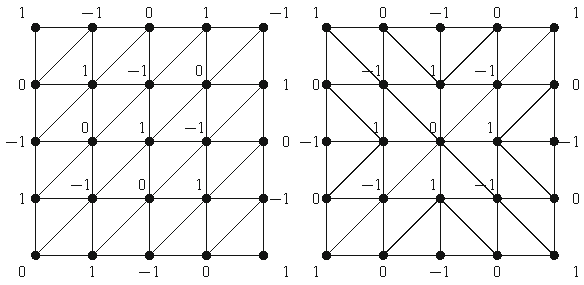
\includegraphics[width=\linewidth]{figures/Chapter_03/Fig_3_01__PDFp077__Bookp065.pdf}
  \captionof{figure}{$P_1/P_1$ 有限元的棋盘格型不稳定模态.}\label{fig:p1p1-checkerboard}
\end{elegantfigure}

\begin{example}[($P_1/P_0$ 有限元空间对)]\label{ex:p1-p0-instability}
正如\hyperref[note:infsup-not-inherited]{注记 3.52} 所指出的,压力有限元空间应当足够小,才能满足离散 inf-sup 条件.由\hyperref[ex:p1-p1-instability]{例题 3.69} 可知,$P_1/P_1$ 空间对显然不满足这一要求.乍看之下,一个直接的想法是用次数更低的多项式逼近压力,也就是用分片常数代替连续分片线性函数.$P_0$ 空间由不连续函数构成,参见\hyperref[ex:appendix-b-37]{例题 B.37}.分片常数函数很容易实现;若 $P_1/P_0$ 空间对满足离散 inf-sup 条件\cref{eq:discrete-infsup-condition},它就会是一个易于使用的选择.

对于 $P_1/P_0$ 空间对,有 $\nabla\cdot P_1\subset P_0$.根据\hyperref[note:mass-conservation-discrete-spaces]{注记 3.56},离散无散速度有限元函数还具有弱无散这一理想性质.然而,$P_1/P_0$ 空间对仍不满足离散 inf-sup 条件\cref{eq:discrete-infsup-condition}.

从\cref{fig:p1p1-checkerboard} 可见,标量值空间 $P_0$ 的维数甚至可能大于标量值空间 $P_1$ 的维数.在图示网格上,$P_1$ 有 25 个自由度(即顶点数),而 $P_0$ 有 32 个自由度(即网格单元数).相应压力有限元空间的自由度各少一个,因为离散压力还必须满足零均值条件.因此可以预期会出现伪模态;下面将详细说明.除此之外,还可能出现另一种称为锁死的现象.

先证明伪模态可能出现.为简单起见,取 $\Omega=(0,1)^2$,考虑\cref{fig:p1p1-checkerboard} 所示类型的网格,其中有 $2n^2$ 个网格单元,$n>1$.速度空间的维数是内部顶点数的两倍,而压力空间的维数等于网格单元数减去零均值约束对应的一个自由度.因此
\[
  \dim V^h-\dim Q^h
   =2(n-1)^2-(2n^2-1)=3-4n<0.
\]
于是,离散系统唯一可解的必要条件 $\dim V^h\ge\dim Q^h$ 不成立,参见\hyperref[note:finite-dimensional-saddle-point]{注记 3.7}.因此,矩阵 $B^h$ 至少有 $4n-3$ 行(等价地,$(B^h)^T$ 至少有 $4n-3$ 列)线性相关.由此可知,$Q^h$ 中存在一个维数至少为 $4n-3$ 的子空间,其中每个 $q^h$ 都满足
\[
  \begin{aligned}
    0&=\bigl\langle (B^h)^Tq^h,v^h\bigr\rangle_{(V^h)',V^h}\\
     &=b^h(v^h,q^h)=-(\nabla\cdot v^h,q^h)
       \qquad\forall v^h\in V^h.
  \end{aligned}
\]
  这正是\cref{eq:spurious-pressure-mode}.将这一例子推广到一般二维多边形区域也是可能的,见\textcite[第 189 页]{ErnGuermond2004}.

\begin{elegantfigure}[0.339\paperwidth]
  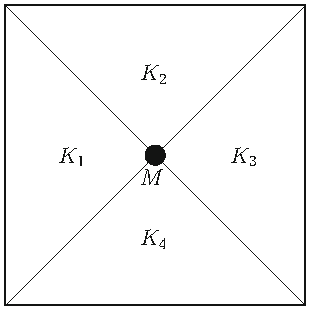
\includegraphics[width=\linewidth]{figures/Chapter_03/Fig_3_02__PDFp078__Bookp066.pdf}
  \captionof{figure}{$P_1/P_0$ 有限元的锁死网格.}\label{fig:p1p0-locking-grid}
\end{elegantfigure}

接下来说明锁死现象.仍取 $\Omega=(0,1)^2$,并用两条对角线将其剖分为四个三角形,如\cref{fig:p1p0-locking-grid} 所示.记分片常数压力检验函数 $q^h$ 在三角形 $K_i$ 上的值为 $q_i^h$,$i=1,\ldots,4$.由于四个三角形面积相等,$q^h\in L_0^2(\Omega)$ 等价于
\[
  q_1^h+q_2^h+q_3^h+q_4^h=0.
\]
因此离散压力有三个独立自由度.由离散无散空间的定义(\cref{eq:discrete-divergence-free-space}),$v^h\in V_{\mathrm{div}}^h$ 必须满足三个独立条件.然而,速度只有两个标量自由度,均位于两条对角线的交点 $M$.设 $v^h=(u^h,v^h)^T$,直接计算得到
\[
  \begin{aligned}
    \left.\nabla\cdot v^h\right|_{K_1}
     &=-\left.\nabla\cdot v^h\right|_{K_3}=\frac{u^h(M)}{2},\\
    \left.\nabla\cdot v^h\right|_{K_4}
     &=-\left.\nabla\cdot v^h\right|_{K_2}=\frac{v^h(M)}{2}.
  \end{aligned}
\]
不妨把 $q_1^h,q_2^h,q_3^h$ 作为离散压力的独立自由度,由上述零均值条件和散度公式可得
\[
\begin{aligned}
  0=(\nabla\cdot v^h,q^h)
   &=|K_1|q_1^h\left.\nabla\cdot v^h\right|_{K_1}\\
   &\quad+|K_1|q_2^h\left.\nabla\cdot v^h\right|_{K_2}\\
   &\quad+|K_1|q_3^h\left.\nabla\cdot v^h\right|_{K_3}\\
   &\quad-|K_1|(q_1^h+q_2^h+q_3^h)
         \left.\nabla\cdot v^h\right|_{K_4}\\
   &=|K_1|u^h(M)\left(\frac{q_1^h}{2}-\frac{q_3^h}{2}\right)\\
   &\qquad-|K_1|v^h(M)
         \left(\frac{q_1^h}{2}+q_2^h+\frac{q_3^h}{2}\right).
\end{aligned}
\]
此式对任意 $q_1^h,q_2^h,q_3^h$ 都成立,故 $u^h(M)=v^h(M)=0$,从而 $V_{\mathrm{div}}^h=\{0\}$.当唯一的离散无散速度是零函数时,就称发生了锁死现象.
\end{example}

\begin{elegantfigure}[0.42\paperwidth]
  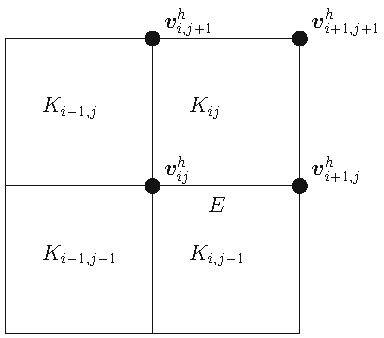
\includegraphics[width=\linewidth]{figures/Chapter_03/Fig_3_03__PDFp079__Bookp067.pdf}
  \captionof{figure}{例题 3.71 中的网格记号.}\label{fig:q1q0-nodal-indexing}
\end{elegantfigure}

\begin{example}[($Q_1/Q_0$ 有限元空间对)]\label{ex:q1-q0-instability}
令 $\Omega=(0,1)^2$,将其剖分为 $n\times n$ 个正方形,其中 $n$ 为偶数.网格单元记为 $K_{ij}$,$i,j=1,\ldots,n$,按从左至右、从下至上的字典序编号.速度有限元函数是双线性分片函数,由其在正方形顶点处的取值确定,参见\hyperref[ex:appendix-b-50]{例题 B.50}.记顶点 $(i,j)$ 处的速度值为 $v_{ij}^h=(u_{ij}^h,v_{ij}^h)^T$,见\cref{fig:q1q0-nodal-indexing}.压力由分片常数有限元函数逼近,参见\hyperref[ex:appendix-b-49]{例题 B.49};记其在 $K_{ij}$ 上的取值为 $q_{ij}^h$.

与在对应网格上将正方形沿对角线剖分所得的 $P_1/P_0$ 有限元相比,速度自由度数相同,因为两种网格的内部顶点数相同.但 $Q_0$ 压力空间的自由度数(网格单元数减一)大约只有相应 $P_0$ 空间的一半.根据\hyperref[note:infsup-not-inherited]{注记 3.52},降低 $Q^h$ 的维数或许能得到满足 inf-sup 条件的空间对.

压力有限元函数的积分均值应为零.设 $h$ 是正方形 $K_{ij}$ 的边长,则 $|K_{ij}|=h^2$,从而
\begin{equation}\label{eq:q1q0-pressure-mean}
  \sum_{i,j=1}^{n}q_{ij}^h=0.
\end{equation}

考虑单个网格单元 $K_{ij}$.分部积分可得
\[
  \int_{K_{ij}}(\nabla\cdot v^h)q_{ij}^h\,\mathrm{d}x
   =q_{ij}^h\int_{K_{ij}}\nabla\cdot v^h\,\mathrm{d}x
   =q_{ij}^h\int_{\partial K_{ij}}v^h\cdot n_{\partial K_{ij}}\,\mathrm{d}s,
\]
其中 $v^h=(u^h,v^h)^T$,$n_{\partial K_{ij}}$ 是 $\partial K_{ij}$ 上指向外侧的单位法向量.边界上的外法向量为 $\pm e_i$($i=1,2$),而 $Q_1$ 有限元函数在每条边上的限制是线性函数,所以边界积分可以用梯形公式精确计算.例如,对底边 $E$ 有
\[
  \int_E v^h\cdot n_{\partial K_{ij}}\,\mathrm{d}s
   =-\int_E v^h\cdot e_2\,\mathrm{d}s
   =-\int_E v_2^h(s)\,\mathrm{d}s
   =-\frac{h}{2}\bigl(v_{ij}^h+v_{i+1,j}^h\bigr).
\]
综合各边的贡献,得到
\[
\begin{aligned}
  \int_{K_{ij}}(\nabla\cdot v^h)q_{ij}^h\,\mathrm{d}x
   =\frac{h}{2}q_{ij}^h\bigl(&-v_{ij}^h-v_{i+1,j}^h
       +u_{i+1,j}^h+u_{i+1,j+1}^h\\
       &+v_{i+1,j+1}^h+v_{i,j+1}^h\\
       &-u_{i,j+1}^h-u_{ij}^h\bigr).
\end{aligned}
\]

接着考察与内部速度节点相关的积分贡献.边界节点不必考虑,因为速度在这些节点处为零.对于节点 $(i,j)$,$i,j=2,\ldots,n$,它是四个网格单元的顶点;这四个单元对积分的贡献分别为
\[
\begin{aligned}
  &\frac{h}{2}u_{ij}^h
     \bigl(q_{i-1,j-1}^h+q_{i-1,j}^h-q_{i,j-1}^h-q_{ij}^h\bigr),\\
  &\frac{h}{2}v_{ij}^h
     \bigl(q_{i-1,j-1}^h+q_{i,j-1}^h-q_{i-1,j}^h-q_{ij}^h\bigr).
\end{aligned}
\]
把所有单元积分相加,只是将求和重新整理为各内部节点的贡献之和.因此,条件\cref{eq:spurious-pressure-mode} 可写成
\[
\begin{aligned}
  0=(\nabla\cdot v^h,q^h)
   &=\sum_{i,j=1}^{n}(\nabla\cdot v^h,q_{ij}^h)_{K_{ij}}\\
   &=\frac{h}{2}\sum_{i,j=2}^{n}u_{ij}^h
       \bigl(q_{i-1,j-1}^h+q_{i-1,j}^h\bigr)\\
   &\quad-\frac{h}{2}\sum_{i,j=2}^{n}u_{ij}^h
       \bigl(q_{i,j-1}^h+q_{ij}^h\bigr)\\
   &\quad+\frac{h}{2}\sum_{i,j=2}^{n}v_{ij}^h
       \bigl(q_{i-1,j-1}^h+q_{i,j-1}^h\bigr)\\
   &\quad-\frac{h}{2}\sum_{i,j=2}^{n}v_{ij}^h
       \bigl(q_{i-1,j}^h+q_{ij}^h\bigr),
       \qquad\forall v^h\in V^h.
\end{aligned}
\]
特别地,令速度有限元函数只有某一个 $u_{ij}^h$ 或 $v_{ij}^h$ 非零,可知压力必须满足
\[
\begin{aligned}
  q_{i-1,j-1}^h+q_{i-1,j}^h-q_{i,j-1}^h-q_{ij}^h&=0,\\
  q_{i-1,j-1}^h+q_{i,j-1}^h-q_{i-1,j}^h-q_{ij}^h&=0,
  \qquad i,j=2,\ldots,n.
\end{aligned}
\]
将这两个条件相加、相减,得到
\begin{equation}\label{eq:q1q0-pressure-recursion}
  q_{ij}^h=q_{i-1,j-1}^h,
  \qquad q_{i,j-1}^h=q_{i-1,j}^h,
  \qquad i,j=2,\ldots,n.
\end{equation}

乍看之下,依据\cref{eq:q1q0-pressure-recursion} 可以自由选取两个压力值:例如令 $K_{11}$ 上的压力为 $\alpha\in\mathbb{R}$,则所有指标和为偶数的网格单元都取同一值;再令另一个网格单元(其指标和为奇数)上的压力为 $\beta$,则另一半网格单元都取此值.假定 $n$ 为偶数,才能使两组网格单元的数量相同.由零均值条件\cref{eq:q1q0-pressure-mean} 可得 $0=\frac{n^2}{2}(\alpha+\beta)$,故 $\beta=-\alpha$.因此,任取 $\alpha\ne0$,便得到满足\cref{eq:spurious-pressure-mode} 的非零压力有限元函数;一个例子见\cref{fig:q1q0-checkerboard}.这种不稳定性也称为棋盘格不稳定.
\end{example}

\begin{elegantfigure}[0.338\paperwidth]
  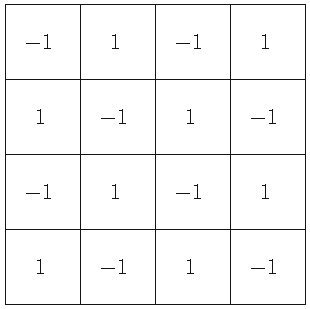
\includegraphics[width=\linewidth]{figures/Chapter_03/Fig_3_04__PDFp081__Bookp069.pdf}
  \captionof{figure}{$Q_1/Q_0$ 有限元的棋盘格型不稳定模态.}\label{fig:q1q0-checkerboard}
\end{elegantfigure}

\begin{note}[改善 $Q_1/Q_0$ 有限元稳定性的改造]\label{note:q1q0-stabilization}
\begin{itemize}
  \item 既然伪模态可以明确刻画,一种做法是缩小压力有限元空间,只保留 $L^2(\Omega)$ 正交于该模态的函数.已有结果表明,这样可以得到满足 inf-sup 条件的有限元空间对.不过,inf-sup 参数依赖于网格宽度,满足 $\beta_{\mathrm{is}}^h=Ch$,其中 $C$ 与 $h$ 无关,参见\textcite[第 II 章第 3 节]{GiraultRaviart1986}.有限元误差估计中会出现 $\beta_{\mathrm{is}}^h$ 的倒数,因此这种方法可能不收敛.
  \item \textcite{BolandNicolaides1985} 提出了对压力有限元空间的进一步改造,使空间对关于 $h$ 一致稳定;细节也可见\textcite[第 167 页]{GiraultRaviart1986}.但据我们所知,Boland 和 Nicolaides 的方法在实践中并未得到应用.
  \item 在非常特殊的网格上,可以证明 $Q_1/Q_0$ 空间对满足离散 inf-sup 条件,见\textcite{Stenberg1984}.
\end{itemize}
\end{note}

\begin{example}[($P_k/P_{k-1}^{\mathrm{disc}}$,$k\ge2$,特殊宏单元)]\label{ex:scott-vogelius-macroelement}
考虑\cref{fig:scott-vogelius-macroelement} 所示网格上的空间对 $P_k/P_{k-1}^{\mathrm{disc}}$,$k\ge2$,特别是粗线框圈出的宏单元.宏单元两条对角线应分别平行于坐标轴.这个空间对称为 Scott--Vogelius 有限元,见\textcite{ScottVogelius1985}.

\begin{elegantfigure}[0.64\paperwidth]
  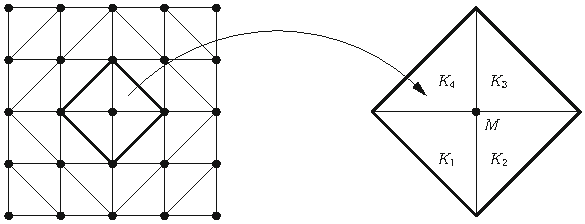
\includegraphics[width=\linewidth]{figures/Chapter_03/Fig_3_05__PDFp082__Bookp070.pdf}
  \captionof{figure}{$P_k/P_{k-1}^{\mathrm{disc}}$ 有限元的网格;粗线框标出宏单元.}\label{fig:scott-vogelius-macroelement}
\end{elegantfigure}

若 $v^h\in P_k$,则 $\nabla\cdot v^h\in P_{k-1}^{\mathrm{disc}}=Q^h$.因此,由\hyperref[note:mass-conservation-discrete-spaces]{注记 3.56} 可知,$P_k/P_{k-1}^{\mathrm{disc}}$ 空间对中的离散无散速度有限元函数也是弱无散的,这是一个理想性质.不过,在图示网格上,$P_k/P_{k-1}^{\mathrm{disc}}$ 并不满足离散 inf-sup 条件.

取 $v^h=(v_1^h,v_2^h)^T\in V_{\mathrm{div}}^h$.由于 $v^h$ 连续,其沿网格边切向的导数 $\nabla v^h\cdot t$ 也连续.利用切向量是笛卡尔坐标单位向量,可得
\[
\begin{aligned}
  \left.\frac{\partial v_2^h}{\partial y}\right|_{K_1}
   &=\left.\frac{\partial v_2^h}{\partial y}\right|_{K_2},
  &\left.\frac{\partial v_1^h}{\partial x}\right|_{K_2}
   &=\left.\frac{\partial v_1^h}{\partial x}\right|_{K_3},\\
  \left.\frac{\partial v_2^h}{\partial y}\right|_{K_3}
   &=\left.\frac{\partial v_2^h}{\partial y}\right|_{K_4},
  &\left.\frac{\partial v_1^h}{\partial x}\right|_{K_4}
   &=\left.\frac{\partial v_1^h}{\partial x}\right|_{K_1}.
\end{aligned}
\]
这些等式在顶点 $M$ 处仍成立.再利用 $K_2,K_3,K_4$ 上逐点散度为零的约束,可得
\[
\begin{aligned}
  \left.\nabla\cdot v^h\right|_{K_1}(M)
   &=\left.\frac{\partial v_1^h}{\partial x}\right|_{K_1}(M)
     +\left.\frac{\partial v_2^h}{\partial y}\right|_{K_1}(M)\\
   &=\left.\frac{\partial v_1^h}{\partial x}\right|_{K_1}(M)
     +\left.\frac{\partial v_2^h}{\partial y}\right|_{K_2}(M)\\
   &=\left.\frac{\partial v_1^h}{\partial x}\right|_{K_1}(M)
     -\left.\frac{\partial v_1^h}{\partial x}\right|_{K_2}(M)\\
   &=\left.\frac{\partial v_1^h}{\partial x}\right|_{K_1}(M)
     -\left.\frac{\partial v_1^h}{\partial x}\right|_{K_3}(M)\\
   &=\left.\frac{\partial v_1^h}{\partial x}\right|_{K_1}(M)
     +\left.\frac{\partial v_2^h}{\partial y}\right|_{K_3}(M)\\
   &=\left.\frac{\partial v_1^h}{\partial x}\right|_{K_1}(M)
     +\left.\frac{\partial v_2^h}{\partial y}\right|_{K_4}(M)\\
   &=\left.\frac{\partial v_1^h}{\partial x}\right|_{K_1}(M)
     -\left.\frac{\partial v_1^h}{\partial x}\right|_{K_4}(M)=0.
\end{aligned}
\]
这说明,$v^h$ 在宏单元 $K_1$ 上的散度为零这一条件,可由边上的切向导数连续性以及 $K_2,K_3,K_4$ 上散度为零推出.由于 $v^h$ 弱无散,故
\begin{equation}\label{eq:scott-vogelius-local-weak-divergence}
  (\nabla\cdot v^h,q^h)_{K_1}=0
  \qquad\forall q^h\in Q^h(K_1).
\end{equation}
由\cref{eq:scott-vogelius-local-weak-divergence} 可知,为确定 $\nabla\cdot v^h|_{K_1}\in P_{k-1}(K_1)$,需要 $\dim P_{k-1}(K_1)=\dim Q^h(K_1)=k(k+1)/2$ 个条件;此外还独立得到 $\nabla\cdot v^h|_{K_1}(M)=0$.因此,\cref{eq:scott-vogelius-local-weak-divergence} 中有一个条件多余.舍去其中一个条件后,$K_1$ 上的一个压力自由度便无法由\cref{eq:scott-vogelius-local-weak-divergence} 确定,成为伪自由度.
\end{example}

\begin{note}[其他网格上的 Scott--Vogelius 有限元]\label{note:scott-vogelius-other-meshes}
例题\hyperref[ex:scott-vogelius-macroelement]{3.73} 中的特殊网格对于证明 Scott--Vogelius 有限元不满足离散 inf-sup 条件至关重要.可以证明,在某种意义下结构性较弱的网格上,次数充分高的 Scott--Vogelius 有限元空间对满足离散 inf-sup 条件,见\hyperref[sec:scott-vogelius]{第 3.6.3 节}.
\end{note}

\begin{note}[绕开离散 inf-sup 条件]\label{note:circumvent-discrete-infsup}
如\hyperref[note:low-order-finite-element-pairs]{注记 3.67} 所述,低阶有限元空间很受欢迎.为将它们用于不可压缩流模拟,人们提出了多种不必满足离散 inf-sup 条件\cref{eq:discrete-infsup-condition} 的方法.其基本思想是在连续性方程中加入双线性型,使压力之间产生耦合,从而消除问题的鞍点结构.第 5.3 节讨论的 PSPG 方法就是一例.当然,在连续性方程中加入额外项会导致(离散)质量守恒遭到破坏.
\end{note}

\section{检验离散 inf-sup 条件的技巧}\label{sec:checking-discrete-infsup}

\begin{note}[内容]\label{note:fortin-section-contents}
本节介绍若干检验离散 inf-sup 条件\cref{eq:discrete-infsup-condition}(或等价的\cref{eq:discrete-infsup-condition-equivalent})的方法,并在第 3.6 节将其中一些方法用于具体的有限元空间对.关于证明离散 inf-sup 条件的技巧及相应结果,较全面的综述可见\textcite{Boffi2008},以及\textcite[第 8.4、8.5 节]{Boffi2013}.
\end{note}

\subsection{Fortin 算子}\label{subsec:fortin-operator}

\begin{note}[连续与离散 inf-sup 条件之间的联系]\label{note:continuous-discrete-infsup-connection}
对于协调有限元空间,可以借助连续 inf-sup 条件\cref{eq:infsup-v-q} 检验离散 inf-sup 条件\cref{eq:discrete-infsup-condition}.下面的引理说明了这两个条件之间的联系.该结果源于\textcite{Fortin1977};它还可推广到 Banach 空间,见\textcite[引理 4.19]{ErnGuermond2004}.某些非协调情形也有相应推广,见第\hyperref[sec:lowest-order-nonconforming]{3.6.5 节}.对于协调有限元空间,$b^h(\cdot,\cdot)=b(\cdot,\cdot)$.
\index{Fortin 算子}
\end{note}

\begin{lemma}[检验离散 inf-sup 条件的 Fortin 判据]\label{lem:fortin-criterion}
设 $V$、$Q$ 和双线性型 $b(\cdot,\cdot)$ 满足注记\hyperref[note:abstract-saddle-point-problem]{3.3} 中的假设,且 inf-sup 条件\cref{eq:infsup-v-q} 成立.考虑协调空间 $V^h\subset V$ 和 $Q^h\subset Q$.则 $V^h$ 与 $Q^h$ 满足离散 inf-sup 条件\cref{eq:discrete-infsup-condition},当且仅当存在一个与 $h$ 无关的常数 $\gamma^h>0$,使得对每个 $v\in V$,都存在 $P_{\mathrm{For}}^h v\in V^h$ 满足
\begin{equation}\label{eq:fortin-property}
  b(v,q^h)=b(P_{\mathrm{For}}^h v,q^h)
  \quad\forall q^h\in Q^h,
  \qquad
  \|P_{\mathrm{For}}^h v\|_V\le \gamma^h\|v\|_V.
\end{equation}
\end{lemma}

\begin{proof}
先假设\cref{eq:fortin-property} 成立.任取 $q^h\in Q^h$.由于 $P_{\mathrm{For}}^h v\in V^h$,利用\cref{eq:fortin-property} 及连续 inf-sup 条件\cref{eq:infsup-v-q},有
\[
\begin{aligned}
  \sup_{v^h\in V^h\setminus\{0\}}
    \frac{b(v^h,q^h)}{\|v^h\|_V}
  &\ge
  \sup_{v\in V\setminus\{0\}}
    \frac{b(P_{\mathrm{For}}^h v,q^h)}
         {\|P_{\mathrm{For}}^h v\|_V}\\
  &=\sup_{v\in V\setminus\{0\}}
    \frac{b(v,q^h)}{\|P_{\mathrm{For}}^h v\|_V}
  \ge \frac{\beta_{\mathrm{is}}}{\gamma^h}
       \|q^h\|_Q .
\end{aligned}
\]
这正是离散 inf-sup 条件\cref{eq:discrete-infsup-condition},且其参数满足 $\beta_{\mathrm{is}}^h\ge \beta_{\mathrm{is}}/\gamma^h$.

反过来,假设离散 inf-sup 条件\cref{eq:discrete-infsup-condition} 成立.将 $b(\cdot,\cdot)$ 从 $V\times Q$ 限制到 $V\times Q^h$,便得到连续线性算子
\[
  \widetilde B\in\mathcal{L}\bigl(V,(Q^h)'\bigr),
  \qquad
  \langle\widetilde Bv,q^h\rangle_{(Q^h)',Q^h}
  :=b(v,q^h).
\]
根据定义,对所有 $v\in V$ 都有 $\widetilde Bv\in(Q^h)'$.由于离散 inf-sup 条件成立,由引理\ref{lem:inf-sup-condition}(iii)可知,\cref{eq:discrete-divergence-operator} 中定义的离散散度算子 $B^h$ 是从 $(V_{\mathrm{div}}^h)^\perp$ 到 $(Q^h)'$ 的同构;特别地,它是满射.于是,对给定的 $v\in V$,存在 $\widetilde v^h\in(V_{\mathrm{div}}^h)^\perp$,使得
\[
  \langle B^h\widetilde v^h,q^h\rangle_{(Q^h)',Q^h}
  =\langle\widetilde Bv,q^h\rangle_{(Q^h)',Q^h}
  \quad\forall q^h\in Q^h.
\]
因此,对所有在 $(V_{\mathrm{div}}^h)^\perp$ 上的正交投影等于 $\widetilde v^h$ 的 $v^h\in V^h$,均有
\begin{equation}\label{eq:fortin-projection-pairing}
  \langle B^h v^h,q^h\rangle_{(Q^h)',Q^h}
  =\langle\widetilde Bv,q^h\rangle_{(Q^h)',Q^h}
  \quad\forall q^h\in Q^h.
\end{equation}
取其中一个这样的函数作为 $P_{\mathrm{For}}^h v$,则\cref{eq:fortin-projection-pairing} 等价于
\[
  b(P_{\mathrm{For}}^h v,q^h)=b(v,q^h)
  \quad\forall q^h\in Q^h.
\]

由引理\ref{lem:inf-sup-condition}(iii)、$Q^h$ 上范数的定义、双线性型 $b(\cdot,\cdot)$ 的范数\cref{eq:bilinear-form-norms},以及其有界性估计(引理\ref{lem:bounded-bilinear-form-b}),可得
\[
\begin{aligned}
  \|P_{\mathrm{For}}^h v\|_V
  &\le \frac{1}{\beta_{\mathrm{is}}^h}
       \|B^hP_{\mathrm{For}}^h v\|_{(Q^h)'}\\
  &=\frac{1}{\beta_{\mathrm{is}}^h}
    \sup_{q^h\in Q^h\setminus\{0\}}
      \frac{\langle B^hP_{\mathrm{For}}^h v,q^h\rangle}
           {\|q^h\|_Q}\\
  &=\frac{1}{\beta_{\mathrm{is}}^h}
    \sup_{q^h\in Q^h\setminus\{0\}}
      \frac{b(v,q^h)}{\|q^h\|_Q}\\
  &\le \frac{\|b\|}{\beta_{\mathrm{is}}^h}\|v\|_V
   =\gamma^h\|v\|_V,
\end{aligned}
\]
从而得到\cref{eq:fortin-property}.证毕.
\end{proof}

\begin{note}[关于条件(3.76)]\label{note:fortin-excludes-spurious-pressure}
条件\cref{eq:spurious-pressure-mode} 一旦成立,就意味着离散 inf-sup 条件被破坏;若\cref{eq:fortin-property} 成立,则不可能满足\cref{eq:spurious-pressure-mode}.事实上,假设存在 $q^h\in Q^h$,使得对所有 $v^h\in V^h$ 都有 $b(v^h,q^h)=0$.由\cref{eq:fortin-property} 可知,对所有 $v\in V$ 都有 $b(v,q^h)=0$,因为 $P_{\mathrm{For}}^h v\in V^h$.又因 $q^h\in Q$,且 $V$ 与 $Q$ 满足 inf-sup 条件\cref{eq:infsup-v-q},故 $q^h=0$.因此,不存在非零的 $q^h\in Q^h$ 满足\cref{eq:spurious-pressure-mode}.
\end{note}

\begin{note}[梯度算子的核]\label{note:fortin-gradient-kernels}
由\cref{eq:fortin-property} 的第一部分可得
\[
  \ker(\operatorname{grad}^h)\subseteq\ker(\operatorname{grad}).
\]
为证此包含关系,取 $q^h\in\ker(\operatorname{grad}^h)$,于是对所有 $v^h\in V^h$,有 $b(v^h,q^h)=0$.由于对每个 $v\in V$ 都有 $P_{\mathrm{For}}^h v\in V^h$,故对所有 $v\in V$ 均有 $b(v,q^h)=0$.因此 $q^h\in\ker(\operatorname{grad})$.
\end{note}

\begin{note}[构造 Fortin 算子的一种方法]\label{note:fortin-construction}
有时可以借助两个线性算子 $P_1^h,P_2^h\in\mathcal{L}(V,V^h)$ 构造线性 Fortin 算子 $P_{\mathrm{For}}^h$.假设
\begin{align}
  \|P_1^h v\|_V&\le C_1\|v\|_V
      &&\forall v\in V,\label{eq:fortin-p1-bound}\\
  \|P_2^h(I-P_1^h)v\|_V&\le C_2\|v\|_V
      &&\forall v\in V,\label{eq:fortin-p2-bound}\\
  b(v-P_2^h v,q^h)&=0
      &&\forall v\in V,\ \forall q^h\in Q^h,\label{eq:fortin-p2-moment}
\end{align}
其中 $C_1,C_2$ 均与 $h$ 无关.定义
\begin{equation}\label{eq:fortin-operator-construction}
  P_{\mathrm{For}}^h\in\mathcal{L}(V,V^h),
  \qquad
  v\longmapsto P_1^h v+P_2^h(v-P_1^h v).
\end{equation}
则 $P_{\mathrm{For}}^h$ 是 Fortin 算子.
\end{note}

\begin{lemma}[算子(3.87)的性质]\label{lem:fortin-operator-construction}
由\cref{eq:fortin-operator-construction} 定义的算子满足\cref{eq:fortin-property}.
\end{lemma}

\begin{proof}
由\cref{eq:fortin-operator-construction},先对 $P_1^h v$ 使用\cref{eq:fortin-p2-moment},再对 $v$ 使用一次\cref{eq:fortin-p2-moment},可得对所有 $q^h\in Q^h$,
\[
\begin{aligned}
  b(P_{\mathrm{For}}^h v,q^h)
  &=b\bigl(P_1^h v+P_2^h(v-P_1^h v),q^h\bigr)\\
  &=b\bigl(P_1^h v-P_2^hP_1^h v,q^h\bigr)
    +b(P_2^h v,q^h)\\
  &=b(P_2^h v,q^h)=b(v,q^h).
\end{aligned}
\]
再由三角不等式以及\cref{eq:fortin-p1-bound,eq:fortin-p2-bound},得到
\[
\begin{aligned}
  \|P_{\mathrm{For}}^h v\|_V
  &\le \|P_1^h v\|_V+
        \|P_2^h(v-P_1^h v)\|_V\\
  &\le C_1\|v\|_V+C_2\|v\|_V
   =\gamma^h\|v\|_V,
\end{aligned}
\qquad\gamma^h:=C_1+C_2.
\]
故\cref{eq:fortin-property} 成立.证毕.
\end{proof}

\begin{note}[Fortin 算子的较精细构造]\label{note:fortin-detailed-construction}
通常可令 $P_1^h$ 取 Clément 插值算子 $P_{\mathrm{Cle}}^h$(\hyperref[eq:appendix-c-17]{式(C.17)}),并作适当修改以保持齐次 Dirichlet 边界条件,见注记\hyperref[note:appendix-c-22]{C.22}.此时,对 $P_2^h$ 的条件\cref{eq:fortin-p2-bound} 可由下列局部估计替代:
\begin{equation}\label{eq:fortin-local-p2-bound}
  \|P_2^h v\|_{H^1(K)}
  \le C\left(h_K^{-1}\|v\|_{L^2(K)}
              +|v|_{H^1(K)}\right),
  \quad\forall K\in\mathcal{T}^h,\ \forall v\in V,
\end{equation}
其中常数 $C$ 与 $h_K$ 无关.
\end{note}

\begin{lemma}[由(C.17)、(3.86)和(3.88)构造的 Fortin 算子的性质]\label{lem:clement-fortin-property}
设 $\{\mathcal{T}^h\}$ 是一族准一致三角剖分(quasi-uniform triangulations).令 $P_1^h=P_{\mathrm{Cle}}^h$ 为经修改、可保持齐次 Dirichlet 边界条件的 Clément 插值算子(\hyperref[eq:appendix-c-17]{C.17}),并设 $P_2^h$ 满足\cref{eq:fortin-p2-moment,eq:fortin-local-p2-bound}.则由\cref{eq:fortin-operator-construction} 定义的 $P_{\mathrm{For}}^h$ 是一个 Fortin 算子.
\end{lemma}

\begin{proof}
\cref{eq:fortin-property} 的第一项性质可按引理\ref{lem:fortin-operator-construction} 的证明得到,因为该证明只用到了\cref{eq:fortin-p2-moment,eq:fortin-operator-construction}.下面证明其中的第二项性质,且所得常数 $\gamma^h$ 与 $h$ 无关.

由剖分族的准一致性可知,对每个 $K$,邻域 $\Omega_K$ 中的网格单元数有一个与剖分无关的上界;此外,$\Omega_K$ 的直径可由 $Ch_K$ 控制,其中常数 $C$ 与 $\mathcal{T}^h$ 无关,见图\hyperref[fig:appendix-c-1]{C.1}.利用\cref{eq:fortin-operator-construction}、三角不等式、\cref{eq:fortin-local-p2-bound},以及在 $k=0,l=1$ 和 $k=l=1$ 时的估计(\hyperref[eq:appendix-c-18]{C.18}),可得
\[
\begin{aligned}
  \|P_{\mathrm{For}}^h v\|_V^2
  &=|P_{\mathrm{For}}^h v|_{H^1(\Omega)}^2\\
  &\le 2|P_{\mathrm{Cle}}^h v|_{H^1(\Omega)}^2
       +2|P_2^h(v-P_{\mathrm{Cle}}^h v)|_{H^1(\Omega)}^2\\
  &\le C\left(|P_{\mathrm{Cle}}^h v-v|_{H^1(\Omega)}^2
                 +|v|_{H^1(\Omega)}^2\right)\\
  &\qquad+2\sum_{K\in\mathcal{T}^h}
        |P_2^h(v-P_{\mathrm{Cle}}^h v)|_{H^1(K)}^2\\
  &\le C\left(\sum_{K\in\mathcal{T}^h}
          |P_{\mathrm{Cle}}^h v-v|_{H^1(K)}^2
          +|v|_{H^1(\Omega)}^2\right)\\
  &\qquad+C\sum_{K\in\mathcal{T}^h}
       \left(h_K^{-2}\|v-P_{\mathrm{Cle}}^h v\|_{L^2(K)}^2
       +|v-P_{\mathrm{Cle}}^h v|_{H^1(K)}^2\right)\\
  &\le C\left(|v|_{H^1(\Omega)}^2
       +3\sum_{K\in\mathcal{T}^h}|v|_{H^1(\Omega_K)}^2\right)\\
  &\le C\|\nabla v\|_{L^2(\Omega)}^2\\
  &=C\|v\|_V^2.
\end{aligned}
\]
证毕.
\end{proof}

\begin{note}[非协调离散]\label{note:fortin-nonconforming}
Fortin 算子的思想也用于非协调方法中证明离散 inf-sup 条件.例如,证明 Crouzeix--Raviart 有限元空间对(见定理\hyperref[thm:crouzeix-raviart-infsup]{3.151})时,就用到了这一思想,相关关系见\hyperref[eq:crouzeix-raviart-fortin-identity]{式(3.144)}和\hyperref[eq:crouzeix-raviart-fortin-bound]{式(3.145)}.
\end{note}

\subsection{将离散压力分解为分片常数部分与余项}\label{subsec:pressure-splitting}

\begin{note}[基本思路]\label{note:pressure-splitting-approach}
注记\hyperref[note:infsup-not-inherited]{3.52} 已指出,较小的压力有限元空间有利于满足离散 inf-sup 条件\cref{eq:discrete-infsup-condition},或等价的\cref{eq:discrete-infsup-condition-equivalent}.给定一个三角剖分,较小的有限元空间是分片常数空间与 $L_0^2(\Omega)$ 的交.这里假设速度空间与分片常数压力空间组成的空间对 $V^h/P_0$ 或 $V^h/Q_0$ 满足离散 inf-sup 条件.然后,将离散 inf-sup 条件\cref{eq:discrete-infsup-condition-equivalent} 右侧的压力有限元函数分解为分片常数部分 $\bar q^h$ 与余项:
\index{分片常数压力空间}
\[
  q^h=\bar q^h+(q^h-\bar q^h).
\]
对于这个余项,也假设有一个 inf-sup 条件,最终由此推出所需的离散 inf-sup 条件.其思路是,分别为分片常数部分和余项证明 inf-sup 条件都相对容易.该方法由\textcite{BrezziBathe1990} 提出.
\end{note}

\begin{lemma}[$L^2(\Omega)$ 投影到分片常数有限元空间的性质]\label{lem:piecewise-constant-projection}
\index{$L^2$ 投影!分片常数空间}
设 $q^h\in Q^h$,并以 $\bar q^h$ 表示它在 $L^2(\Omega)$ 中到 $P_0$ 或 $Q_0$ 的投影,即
\begin{equation}\label{eq:piecewise-constant-projection-orthogonality}
  (q^h-\bar q^h,r^h)=0
  \qquad\forall r^h\in P_0\ (\text{或 }Q_0).
\end{equation}
则
\[
  \left.\bar q^h\right|_K
  =\frac{1}{|K|}\int_K q^h(x)\,\mathrm{d}x
  \qquad\forall K\in\mathcal{T}^h,
\]
其中 $|K|$ 表示 $K$ 的测度,并且 $\bar q^h\in L_0^2(\Omega)$.
\end{lemma}

\begin{proof}
利用 $\bar q^h$ 和 $r^h$ 都是分片常数,有
\[
\begin{aligned}
  (q^h,r^h)
  &=\sum_{K\in\mathcal{T}^h}(q^h,r^h)_K\\
  &=\sum_{K\in\mathcal{T}^h}
      \left.r^h\right|_K\int_K q^h(x)\,\mathrm{d}x,
\end{aligned}
\]
另一方面,
\[
\begin{aligned}
  (\bar q^h,r^h)
  &=\sum_{K\in\mathcal{T}^h}(\bar q^h,r^h)_K\\
  &=\sum_{K\in\mathcal{T}^h}
      \left.r^h\right|_K\left.\bar q^h\right|_K|K|.
\end{aligned}
\]
将这两个表达式代入\cref{eq:piecewise-constant-projection-orthogonality},即得 $\bar q^h|_K$ 的公式.再利用该公式以及 $q^h\in L_0^2(\Omega)$,可知 $\bar q^h$ 的均值为零:
\[
\begin{aligned}
  \int_\Omega\bar q^h(x)\,\mathrm{d}x
  &=\sum_{K\in\mathcal{T}^h}\int_K\bar q^h(x)\,\mathrm{d}x\\
  &=\sum_{K\in\mathcal{T}^h}
      \left.\bar q^h\right|_K\int_K\mathrm{d}x\\
  &=\sum_{K\in\mathcal{T}^h}
      \frac{1}{|K|}\int_Kq^h(x)\,\mathrm{d}x\int_K\mathrm{d}x\\
  &=\int_\Omega q^h(x)\,\mathrm{d}x=0.
\end{aligned}
\]
证毕.
\end{proof}

\begin{note}[一种改进的 inf-sup 条件]\label{note:modified-infsup-condition}
\index{改进的 inf-sup 条件}
这种方法的核心是如下形式的 inf-sup 条件:
\begin{equation}\label{eq:modified-infsup-condition}
  \sup_{v^h\in V^h\setminus\{0\}}
    \frac{b^h(v^h,q^h)}{\|v^h\|_{V^h}}
  \ge\beta_1\|q^h-\bar q^h\|_Q
  \qquad\forall q^h\in Q^h,
\end{equation}
其中 $\beta_1>0$ 与网格宽度无关.由引理\ref{lem:piecewise-constant-projection} 可知,$q^h-\bar q^h\in L_0^2(\Omega)$.首先,由这一表述可见,若能找到满足\cref{eq:spurious-pressure-mode} 的 $q^h\in Q^h$,则\cref{eq:modified-infsup-condition} 不可能成立:此时左端为零,而在本节假设分片常数压力空间对稳定的前提下,右端不为零.因此,\cref{eq:modified-infsup-condition} 可排除足以说明 $V^h/Q^h$ 不满足离散 inf-sup 条件的情形.另一方面,\cref{eq:modified-infsup-condition} 弱于离散 inf-sup 条件.为简单起见,考虑准一致网格.由 $L^2(\Omega)$ 投影的性质(\hyperref[eq:appendix-c-28]{C.28})和逆不等式(\hyperref[eq:appendix-c-35]{C.35}),有
\[
\begin{aligned}
  \|q^h-\bar q^h\|_Q
  &=\left(\sum_{K\in\mathcal{T}^h}
        \|q^h-\bar q^h\|_{L^2(K)}^2\right)^{1/2}\\
  &\le C\left(\sum_{K\in\mathcal{T}^h}
        h_K^2\|\nabla q^h\|_{L^2(K)}^2\right)^{1/2}\\
  &\le C\left(\sum_{K\in\mathcal{T}^h}
        \|q^h\|_{L^2(K)}^2\right)^{1/2}
   =C\|q^h\|_Q.
\end{aligned}
\]
因此,若\cref{eq:discrete-infsup-condition}(或等价的\cref{eq:discrete-infsup-condition-equivalent})成立,则\cref{eq:modified-infsup-condition} 也成立.
\end{note}

\begin{theorem}[基于分片常数压力 inf-sup 条件的离散 inf-sup 条件充分条件]\label{thm:pressure-splitting-infsup}
假设速度空间与分片常数压力空间 $V^h/P_0$ 或 $V^h/Q_0$ 满足离散 inf-sup 条件
\begin{equation}\label{eq:piecewise-constant-infsup}
  \sup_{v^h\in V^h\setminus\{0\}}
    \frac{b^h(v^h,q^h)}{\|v^h\|_{V^h}}
  \ge\beta_0\|q^h\|_Q
  \qquad\forall q^h\in P_0\ (\text{或 }Q_0),
\end{equation}
其中 $\beta_0>0$ 与 $h$ 无关.此外,假设\cref{eq:modified-infsup-condition} 成立,且 $\beta_1$ 与 $h$ 无关.则离散 inf-sup 条件\cref{eq:discrete-infsup-condition} 或\cref{eq:discrete-infsup-condition-equivalent} 成立,并且其参数满足
\[
  \beta_{\mathrm{is}}^h
  =\frac{\beta_0\beta_1}{\widetilde C+\beta_0+\beta_1}>0,
\]
其中协调速度空间对应 $\widetilde C=1$,非协调速度空间对应 $\widetilde C=\sqrt{d}$.
\end{theorem}

\begin{proof}
由于和的上确界不大于各项上确界之和,有
\[
  \sup A=\sup\bigl((A+B)-B\bigr)
  \le \sup(A+B)+\sup B,
\]
从而
\begin{equation}\label{eq:sup-sum-lower-bound}
  \sup(A+B)\ge\sup A-\sup B.
\end{equation}
任取 $q^h\in Q^h$.将压力分解为 $\bar q^h+(q^h-\bar q^h)$,并应用\cref{eq:sup-sum-lower-bound,eq:piecewise-constant-infsup} 以及协调速度空间情形的估计(3.41)或非协调速度空间情形的估计(3.40),得到
\begin{equation}\label{eq:pressure-splitting-infsup-first-estimate}
\begin{aligned}
  \sup_{v^h\in V^h\setminus\{0\}}
    \frac{b^h(v^h,q^h)}{\|v^h\|_{V^h}}
  &\ge
    \sup_{v^h\in V^h\setminus\{0\}}
      \frac{b^h(v^h,\bar q^h)}{\|v^h\|_{V^h}}\\
  &\qquad-
    \sup_{v^h\in V^h\setminus\{0\}}
      \frac{b^h(v^h,q^h-\bar q^h)}{\|v^h\|_{V^h}}\\
  &\ge \beta_0\|\bar q^h\|_Q\\
  &\qquad-
    \sup_{v^h\in V^h\setminus\{0\}}
        \frac{\|\nabla\cdot v^h\|_{L^2(\Omega)}
              \|q^h-\bar q^h\|_Q}{\|v^h\|_{V^h}}\\
  &\ge \beta_0\|\bar q^h\|_Q
      -\widetilde C\|q^h-\bar q^h\|_Q.
\end{aligned}
\end{equation}
对于非协调速度有限元空间,第二行中的 $\|\nabla\cdot v^h\|_{L^2(\Omega)}$ 应改为各网格单元上的相应范数平方和,并在每个单元上应用估计(3.40).

现在结合\cref{eq:modified-infsup-condition,eq:pressure-splitting-infsup-first-estimate},可得
\[
\begin{aligned}
  \sup_{v^h\in V^h\setminus\{0\}}
    \frac{b^h(v^h,q^h)}{\|v^h\|_{V^h}}
  &\ge \beta_1\|q^h-\bar q^h\|_Q\\
  &\ge \beta_1\left(
      \frac{\beta_0}{\widetilde C}\|\bar q^h\|_Q
      -\frac{1}{\widetilde C}
       \sup_{v^h\in V^h\setminus\{0\}}
        \frac{b^h(v^h,q^h)}{\|v^h\|_{V^h}}
       \right).
\end{aligned}
\]
移项后得到
\begin{equation}\label{eq:pressure-splitting-mean-infsup}
  \sup_{v^h\in V^h\setminus\{0\}}
    \frac{b^h(v^h,q^h)}{\|v^h\|_{V^h}}
  \ge
  \frac{\beta_0\beta_1}{\widetilde C+\beta_1}
       \|\bar q^h\|_Q.
\end{equation}

再在\cref{eq:modified-infsup-condition} 中使用三角不等式,并代入\cref{eq:pressure-splitting-mean-infsup},可得
\[
\begin{aligned}
  \sup_{v^h\in V^h\setminus\{0\}}
    \frac{b^h(v^h,q^h)}{\|v^h\|_{V^h}}
  &\ge \beta_1\|q^h\|_Q-\beta_1\|\bar q^h\|_Q\\
  &\ge \beta_1\|q^h\|_Q
   -\frac{\widetilde C+\beta_1}{\beta_0}
      \sup_{v^h\in V^h\setminus\{0\}}
        \frac{b^h(v^h,q^h)}{\|v^h\|_{V^h}}.
\end{aligned}
\]
将最后一项移至左侧,并注意 $q^h$ 任意,便得到定理陈述中的离散 inf-sup 条件及其参数 $\beta_{\mathrm{is}}^h$.证毕.
\end{proof}

\begin{note}[关于条件(3.90)]\label{note:modified-infsup-condition-comments}
\index{拼块检验}
\begin{itemize}
  \item \textcite{BrezziBathe1990} 提出了一种所谓的拼块检验,用于检验条件\cref{eq:modified-infsup-condition}.
\item \textcite{BrezziBathe1990} 还给出了另一种情形,在该情形下条件\cref{eq:modified-infsup-condition} 可推出离散 inf-sup 条件,见定理\hyperref[thm:brezzi-bathe-continuous-pressure]{3.96}.
\end{itemize}
\end{note}

\subsection{协调速度空间与连续压力空间的方法}\label{subsec:conforming-velocity-continuous-pressure}

\begin{note}[内容]\label{note:continuous-pressure-criteria}
\index{连续压力空间}
本节介绍两种判据,用于在压力空间由连续有限元函数(continuous finite element functions)组成时检验离散 inf-sup 条件\cref{eq:discrete-infsup-condition} 或\cref{eq:discrete-infsup-condition-equivalent}.第一种判据由 Verfürth(1984)证明,第二种由 Brezzi 和 Bathe(1990)证明;可以看出,这两种判据在一定程度上等价.

\index{分部积分}
\index{压力跳跃}
本节为推导离散 inf-sup 条件,需要对连续函数 $v$ 与离散压力 $q^h$ 所构成的项 $b^h(v,q^h)$ 作分部积分(integration by parts).一般而言,这会产生网格单元各个面的离散压力跳跃项(jumps of the discrete pressure);压力空间的光滑性假设 $Q^h\subset H^1(\Omega)$ 保证这些跳跃项为零.

以下假设 $V^h\subset V$,因此 $b^h(\cdot,\cdot)=b(\cdot,\cdot)$ 且 $\|\cdot\|_{V^h}=\|\cdot\|_V$.
\end{note}

\begin{lemma}[上确界的下界]\label{lem:continuous-pressure-supremum-lower-bound}
设 $\{\mathcal{T}^h\}$ 是准一致三角剖分族,且 $V^h\subset V$、$Q^h\subset H^1(\Omega)$.假设存在线性算子 $P_1^h:V\to V^h$,使得
\begin{equation}\label{eq:continuous-pressure-interpolant-error}
\begin{aligned}
  \|v-P_1^h v\|_{H^k(\Omega)}
  &\le C\left(
    \sum_{K\in\mathcal{T}^h}
       h_K^{2-2k}\|\nabla v\|_{L^2(K)}^2
       \right)^{1/2},\\
  &\qquad\forall v\in V,\quad k=0,1.
\end{aligned}
\end{equation}
其中 $C>0$ 与网格宽度无关.则存在常数 $C_1,C_2>0$,使得对每个 $q^h\in Q^h$,
\begin{equation}\label{eq:continuous-pressure-discrete-infsup-lower-bound}
\begin{aligned}
  \sup_{w^h\in V^h\setminus\{0\}}
    \frac{b(w^h,q^h)}{\|w^h\|_V}
  &\ge C_1\|q^h\|_Q
      \\
  &\qquad-C_2\left(
       \sum_{K\in\mathcal{T}^h}
           h_K^2\|\nabla q^h\|_{L^2(K)}^2
       \right)^{1/2}.
\end{aligned}
\end{equation}
\end{lemma}

\begin{proof}
任取 $q^h\in Q^h\subset Q$.由推论\ref{cor:each-pressure-is-divergence},存在 $v\in V$,使得 $\nabla\cdot v=q^h$,且 $\|v\|_V\le C_3\|q^h\|_Q$,其中 $C_3$ 与 $v$、$q^h$ 无关.

对这个 $v$,在分母中使用三角不等式和\cref{eq:continuous-pressure-interpolant-error}($k=1$),在分子中使用三角不等式,得到
\begin{equation}\label{eq:continuous-pressure-interpolant-sup-estimate}
\begin{aligned}
  \sup_{v^h\in V^h\setminus\{0\}}
    \frac{b(v^h,q^h)}{\|v^h\|_V}
  &\ge
    \frac{|b(P_1^h v,q^h)|}{\|P_1^h v\|_V}\\
  &\ge
    \frac{|b(P_1^h v,q^h)|}
         {\|v\|_V+\|v-P_1^h v\|_V}\\
  &\ge \frac{1}{1+C}
       \frac{|b(P_1^h v,q^h)|}{\|v\|_V}\\
  &\ge \frac{1}{1+C}
       \left(
         \frac{|b(v,q^h)|}{\|v\|_V}
         -\frac{|b(v-P_1^h v,q^h)|}{\|v\|_V}
       \right).
\end{aligned}
\end{equation}
对于第一项,由 $\nabla\cdot v=q^h$ 及推论\ref{cor:each-pressure-is-divergence} 的估计,有
\[
  \frac{|b(v,q^h)|}{\|v\|_V}
  =\frac{\|q^h\|_Q^2}{\|v\|_V}
  \ge\frac{1}{C_3}\|q^h\|_Q.
\]

对于第二项,作分部积分可得
\[
\begin{aligned}
  (\nabla\cdot(v-P_1^h v),q^h)
  &=\sum_{K\in\mathcal{T}^h}
       (\nabla\cdot(v-P_1^h v),q^h)_K\\
  &=\sum_{K\in\mathcal{T}^h}\left[
       -(\nabla q^h,v-P_1^h v)_K\right.\\
  &\qquad\left.+\int_{\partial K}
          q^h(v-P_1^h v)\cdot n_{\partial K}\,\mathrm{d}s
       \right].
\end{aligned}
\]
离散速度空间和压力空间的正则性条件保证各面上的边界积分相互抵消.应用 Cauchy--Schwarz 不等式(\hyperref[eq:appendix-a-10]{A.10})、和式的 Cauchy--Schwarz 不等式(\hyperref[eq:appendix-a-2]{A.2})、\cref{eq:continuous-pressure-interpolant-error}($k=0$),以及剖分族的准一致性,有
\[
  \begin{aligned}
    \frac{|b(v-P_1^h v,q^h)|}{\|v\|_V}
    &=\frac{|(\nabla q^h,v-P_1^h v)|}{\|v\|_V}\\
    &\le
      \frac{1}{\|v\|_V}
      \sum_{K\in\mathcal{T}^h}
         \left(h_K\|\nabla q^h\|_{L^2(K)}\right)\\
    &\qquad\times
         \left(h_K^{-1}\|v-P_1^h v\|_{L^2(K)}\right)\\
    &\le \frac{1}{\|v\|_V}
       \left(\sum_{K\in\mathcal{T}^h}
             h_K^2\|\nabla q^h\|_{L^2(K)}^2\right)^{1/2}\\
    &\qquad\times
       \left(\sum_{K\in\mathcal{T}^h}
             h_K^{-2}\|v-P_1^h v\|_{L^2(K)}^2\right)^{1/2}\\
    &\le
      \left(\min_{K\in\mathcal{T}^h}h_K\right)^{-1}
      \left(\sum_{K\in\mathcal{T}^h}
         h_K^2\|\nabla q^h\|_{L^2(K)}^2\right)^{1/2}\\
    &\qquad\times
      \frac{\|v-P_1^h v\|_{L^2(\Omega)}}{\|v\|_V}\\
    &\le C
      \left(\min_{K\in\mathcal{T}^h}h_K\right)^{-1}
      \left(\sum_{K\in\mathcal{T}^h}
         h_K^2\|\nabla q^h\|_{L^2(K)}^2\right)^{1/2}\\
    &\qquad\times
      \frac{\left(\sum_{K\in\mathcal{T}^h}
         h_K^2\|\nabla v\|_{L^2(K)}^2\right)^{1/2}}
           {\|v\|_V}\\
    &\le C
        \frac{\max_{K\in\mathcal{T}^h}h_K}
             {\min_{K\in\mathcal{T}^h}h_K}\\
    &\qquad\times
        \left(\sum_{K\in\mathcal{T}^h}
           h_K^2\|\nabla q^h\|_{L^2(K)}^2\right)^{1/2}\\
  &\le C
    \left(\sum_{K\in\mathcal{T}^h}
       h_K^2\|\nabla q^h\|_{L^2(K)}^2\right)^{1/2}.
\end{aligned}
\]
将上述估计代入\cref{eq:continuous-pressure-interpolant-sup-estimate},即得\cref{eq:continuous-pressure-discrete-infsup-lower-bound},其中
\[
  C_1=\frac{1}{C_3(1+C)},
  \qquad
  C_2=\frac{C}{1+C}.
\]
证毕.
\end{proof}

\begin{note}[算子 $P_1^h$ 的一种选择]\label{note:clement-as-p1}
Verfürth(1984)已指出,可以令 $P_1^h$ 取 Clément 插值算子 $P_{\mathrm{Cle}}^h$(\hyperref[eq:appendix-c-17]{C.17}),并作注记\hyperref[note:appendix-c-22]{C.22} 所述的修改以保持齐次 Dirichlet 边界条件.
\end{note}

\begin{theorem}[Verfürth(1984)的连续压力空间离散 inf-sup 条件判据]\label{thm:verfurth-continuous-pressure}
假设引理\ref{lem:continuous-pressure-supremum-lower-bound} 的条件成立.此外,假设如下形式的 inf-sup 条件成立:
\begin{equation}\label{eq:continuous-pressure-gradient-infsup}
\begin{aligned}
  \sup_{v^h\in V^h\setminus\{0\}}
    \frac{b(v^h,q^h)}{\|v^h\|_V}
  &\ge \beta_2
       \left(\sum_{K\in\mathcal{T}^h}
          h_K^2\|\nabla q^h\|_{L^2(K)}^2\right)^{1/2}\\
  &\qquad\forall q^h\in Q^h.
\end{aligned}
\end{equation}
则离散 inf-sup 条件\cref{eq:discrete-infsup-condition},或等价的\cref{eq:discrete-infsup-condition-equivalent},成立.
\end{theorem}

\begin{proof}
将 $\beta_2$ 倍的\cref{eq:continuous-pressure-discrete-infsup-lower-bound} 与 $C_2$ 倍的\cref{eq:continuous-pressure-gradient-infsup} 相加,得到
\[
  (\beta_2+C_2)
  \sup_{v^h\in V^h\setminus\{0\}}
    \frac{b(v^h,q^h)}{\|v^h\|_V}
  \ge C_1\beta_2\|q^h\|_Q.
\]
因此,\cref{eq:discrete-infsup-condition-equivalent} 成立,其参数为
\[
  \beta_{\mathrm{is}}^h
  =\frac{C_1\beta_2}{\beta_2+C_2}.
\]
证毕.
\end{proof}

\begin{corollary}[满足条件(3.98)的判据]\label{cor:continuous-pressure-gradient-infsup}
设 $\{\mathcal{T}^h\}$ 是准一致三角剖分族.若对每个 $q^h\in Q^h$,都存在 $v^h\in V^h$ 及正常数 $C_1,C_2$,使得
\begin{equation}\label{eq:continuous-pressure-gradient-test}
  b(v^h,q^h)\ge C_1\|\nabla q^h\|_{L^2(\Omega)}^2,
  \qquad
  \|v^h\|_{L^2(\Omega)}^2
  \le C_2\|\nabla q^h\|_{L^2(\Omega)}^2,
\end{equation}
其中 $C_1,C_2$ 与 $q^h$ 及网格宽度均无关,
则条件\cref{eq:continuous-pressure-gradient-infsup} 成立.
\end{corollary}

\begin{proof}
由逆不等式(\hyperref[eq:appendix-c-37]{C.37})及假设\cref{eq:continuous-pressure-gradient-test},取其中保证存在的函数 $v^h$.若 $\|\nabla q^h\|_{L^2(\Omega)}=0$,结论显然成立;否则,
\[
\begin{aligned}
  \sup_{w^h\in V^h\setminus\{0\}}
    \frac{b(w^h,q^h)}{\|w^h\|_V}
  &\ge C\frac{b(v^h,q^h)}
           {h^{-1}\|v^h\|_{L^2(\Omega)}}\\
  &\ge Ch\frac{C_1\|\nabla q^h\|_{L^2(\Omega)}^2}
           {\sqrt{C_2}\|\nabla q^h\|_{L^2(\Omega)}}\\
  &=\frac{C C_1}{\sqrt{C_2}}h\|\nabla q^h\|_{L^2(\Omega)}.
\end{aligned}
\]
准一致三角剖分族上,这给出\cref{eq:continuous-pressure-gradient-infsup}.证毕.
\end{proof}

\begin{theorem}[连续压力空间判据(Brezzi--Bathe,1990)]\label{thm:brezzi-bathe-continuous-pressure}
设 $V^h\subset V$、$Q^h\subset H^1(\Omega)$,且考虑一个准一致三角剖分族.此外,假设对每个 $v\in V$,都存在插值函数(interpolant)$v_I^h\in V^h$,满足
\begin{align}
  \|v-v_I^h\|_{L^2(\Omega)}
  &\le Ch\|v\|_V,\label{eq:brezzi-bathe-interpolant-l2}\\
  \|v_I^h\|_V
  &\le C\|v\|_V,\label{eq:brezzi-bathe-interpolant-v}
\end{align}
其中常数与剖分无关.若\cref{eq:modified-infsup-condition} 也成立,则 $V^h/Q^h$ 满足离散 inf-sup 条件\cref{eq:discrete-infsup-condition},或等价的\cref{eq:discrete-infsup-condition-equivalent}.
\end{theorem}

\begin{proof}
由 $V^h$ 和 $Q^h$ 的正则性条件,对所有 $v\in V$ 分部积分可得
\begin{equation}\label{eq:brezzi-bathe-integration-by-parts}
\begin{aligned}
  b(v_I^h-v,q^h)
  &=-\sum_{K\in\mathcal{T}^h}
       \int_K\nabla\cdot(v_I^h-v)\,q^h\,\mathrm{d}x\\
  &=\sum_{K\in\mathcal{T}^h}\left[
       -\int_{\partial K}q^h(v_I^h-v)\cdot n_{\partial K}\,\mathrm{d}s\right.\\
  &\qquad\left.+\int_K(v_I^h-v)\cdot\nabla q^h\,\mathrm{d}x
       \right]\\
  &=(\nabla q^h,v_I^h-v).
\end{aligned}
\end{equation}

任取 $q^h\in Q^h\subset Q$.由于空间对 $V/Q$ 满足连续 inf-sup 条件\cref{eq:infsup-v-q},存在 $\widetilde v\in V$,使得
\begin{equation}\label{eq:brezzi-bathe-continuous-infsup-witness}
  \frac{b(\widetilde v,q^h)}{\|\widetilde v\|_V}
  \ge(\beta_{\mathrm{is}}-\varepsilon)\|q^h\|_Q
\end{equation}
其中 $\varepsilon\in(0,\beta_{\mathrm{is}}/2)$ 可任意选取.记 $\widetilde\beta_{\mathrm{is}}:=\beta_{\mathrm{is}}-\varepsilon>0$.在上确界中取特殊函数 $v_I^h$,并注意到改取其相反数时上确界也不减;再应用\cref{eq:brezzi-bathe-interpolant-v}、三角不等式、\cref{eq:brezzi-bathe-continuous-infsup-witness,eq:brezzi-bathe-integration-by-parts}、Cauchy--Schwarz 不等式(A.10)和\cref{eq:brezzi-bathe-interpolant-l2},得到
\begin{equation}\label{eq:brezzi-bathe-interpolant-sup-estimate}
\begin{aligned}
  \sup_{v^h\in V^h\setminus\{0\}}
    \frac{b(v^h,q^h)}{\|v^h\|_V}
  &\ge
    \frac{|b(v_I^h,q^h)|}{\|v_I^h\|_V}
   \ge C\frac{|b(v_I^h,q^h)|}{\|\widetilde v\|_V}\\
  &\ge C\left(
       -\frac{|b(v_I^h-\widetilde v,q^h)|}{\|\widetilde v\|_V}
       +\frac{|b(\widetilde v,q^h)|}{\|\widetilde v\|_V}
       \right)\\
  &\ge C\left(
       -\frac{|b(v_I^h-\widetilde v,q^h)|}{\|\widetilde v\|_V}
       +\widetilde\beta_{\mathrm{is}}\|q^h\|_Q
       \right)\\
  &=C\left(
       -\frac{|(\nabla q^h,v_I^h-\widetilde v)|}
              {\|\widetilde v\|_V}
       +\widetilde\beta_{\mathrm{is}}\|q^h\|_Q
       \right)\\
  &\ge C\left(
       \widetilde\beta_{\mathrm{is}}\|q^h\|_Q
       -h\|\nabla q^h\|_{L^2(\Omega)}
       \right).
\end{aligned}
\end{equation}

令 $\bar q^h$ 为\cref{eq:piecewise-constant-projection-orthogonality} 所定义的 $L^2(\Omega)$ 投影.由于每个网格单元上 $\nabla\bar q^h=0$,利用逆不等式(\hyperref[eq:appendix-c-35]{C.35})和剖分族的准一致性可得
\[
\begin{aligned}
  \|\nabla q^h\|_{L^2(\Omega)}
  &=\left(\sum_{K\in\mathcal{T}^h}
       \|\nabla(q^h-\bar q^h)\|_{L^2(K)}^2\right)^{1/2}\\
  &\le C\left(\sum_{K\in\mathcal{T}^h}
       h_K^{-2}\|q^h-\bar q^h\|_{L^2(K)}^2\right)^{1/2}\\
  &\le Ch^{-1}\|q^h-\bar q^h\|_Q.
\end{aligned}
\]
将此估计代入\cref{eq:brezzi-bathe-interpolant-sup-estimate},再使用\cref{eq:modified-infsup-condition},得到
\[
  \sup_{v^h\in V^h\setminus\{0\}}
    \frac{b(v^h,q^h)}{\|v^h\|_V}
  \ge C\widetilde\beta_{\mathrm{is}}\|q^h\|_Q
       -\frac{C}{\beta_1}
        \sup_{v^h\in V^h\setminus\{0\}}
          \frac{b(v^h,q^h)}{\|v^h\|_V}.
\]
将最后一项移至左侧,并除以左侧所得的系数,即完成证明.证毕.
\end{proof}

\begin{note}[假设(3.90)和(3.98)的等价性]\label{note:modified-gradient-infsup-equivalence}
类似于定理\ref{thm:brezzi-bathe-continuous-pressure} 的证明,利用逆不等式(\hyperref[eq:appendix-c-35]{C.35})可得
\[
\begin{aligned}
  \left(\sum_{K\in\mathcal{T}^h}
       h_K^2\|\nabla q^h\|_{L^2(K)}^2\right)^{1/2}
  &=\left(\sum_{K\in\mathcal{T}^h}
       h_K^2\|\nabla(q^h-\bar q^h)\|_{L^2(K)}^2\right)^{1/2}\\
  &\le C_{\mathrm{inv}}\|q^h-\bar q^h\|_Q.
\end{aligned}
\]
另一方面,由 $L^2(\Omega)$ 到分片常数有限元函数空间的投影性质(\hyperref[eq:appendix-c-28]{C.28})可知,
\[
\begin{aligned}
  \|q^h-\bar q^h\|_Q
  &=\left(\sum_{K\in\mathcal{T}^h}
       \|q^h-\bar q^h\|_{L^2(K)}^2\right)^{1/2}\\
  &\le C\left(\sum_{K\in\mathcal{T}^h}
       h_K^2\|\nabla q^h\|_{L^2(K)}^2\right)^{1/2}.
\end{aligned}
\]
因此,条件\cref{eq:modified-infsup-condition,eq:continuous-pressure-gradient-infsup} 等价.特别地,注记\ref{note:modified-infsup-condition} 对条件(3.90)的讨论同样适用于条件(3.98).
\end{note}

\begin{note}[定理 3.94 推出定理 3.96]\label{note:verfurth-implies-brezzi-bathe}
若定理\ref{thm:verfurth-continuous-pressure} 的假设成立,则定理\ref{thm:brezzi-bathe-continuous-pressure} 的假设也成立.条件\cref{eq:modified-infsup-condition} 与\cref{eq:continuous-pressure-gradient-infsup} 的等价性已在注记\ref{note:modified-gradient-infsup-equivalence} 中说明.由算子 $P_1^h$ 满足的条件\cref{eq:continuous-pressure-interpolant-error} 可知,对于准一致三角剖分族,
\[
  \|v-P_1^h v\|_{L^2(\Omega)}
  \le Ch\|\nabla v\|_{L^2(\Omega)}
  =Ch\|v\|_V,
\]
并且
\[
\begin{aligned}
  \|P_1^h v\|_V
  &=\|\nabla P_1^h v\|_{L^2(\Omega)}\\
  &\le \|\nabla(v-P_1^h v)\|_{L^2(\Omega)}
       +\|\nabla v\|_{L^2(\Omega)}\\
  &\le (C+1)\|\nabla v\|_{L^2(\Omega)}
   =C\|v\|_V.
\end{aligned}
\]
因此,令 $v_I^h=P_1^h v$,即可满足定理\ref{thm:brezzi-bathe-continuous-pressure} 中的条件\cref{eq:brezzi-bathe-interpolant-l2,eq:brezzi-bathe-interpolant-v}.
\end{note}

\subsection{宏单元方法}\label{subsec:macroelement-techniques}

\begin{note}[目标]\label{note:macroelement-goal}
\index{宏单元方法}
\index{局部 inf-sup 条件}
宏单元方法(macroelement techniques)旨在将离散 inf-sup 条件的证明归结为局部 inf-sup 条件(local inf-sup condition)的证明.这类方法由\textcite{BolandNicolaides1983} 以及\textcite{Stenberg1984,Stenberg1987,Stenberg1990} 提出.
\end{note}

\clearpage
\begin{note}[Boland 和 Nicolaides(1983)的方法]\label{note:boland-nicolaides-approach}
该方法将区域 $\Omega$ 分解为两两不交的开子域 $\Omega_r$($r=1,\ldots,R$),使得
\[
  \overline{\Omega}=\bigcup_{r=1}^{R}\overline{\Omega_r},
  \qquad
  \Omega_r\cap\Omega_s=\varnothing\quad(r\ne s).
\]
利用全局有限元空间 $V^h$ 和 $Q^h$,在每个 $\Omega_r$ 上定义局部空间
\[
\begin{aligned}
  V^h(\Omega_r)
  &=\left\{v^h|_{\Omega_r}:v^h\in V^h,\quad
         v^h=0\text{ 于 }\Omega\setminus\Omega_r\right\},\\
  Q^h(\Omega_r)
  &=\left\{q^h|_{\Omega_r}:q^h\in Q^h\cap L_0^2(\Omega_r)\right\}.
\end{aligned}
\]
此外,还需要由分片常数函数组成的全局压力有限元空间
\[
  Q_0^h
  =\left\{q^h\in L_0^2(\Omega):
       q^h|_{\Omega_r}\in P_0(\Omega_r),\quad r=1,\ldots,R\right\}.
\]
现在可以表述局部离散 inf-sup 条件:存在与网格宽度 $h$ 无关的常数 $\beta_{\mathrm{is,loc}}^h>0$,使得对所有 $r=1,\ldots,R$,
\begin{equation}\label{eq:macroelement-local-infsup}
  \inf_{q^h\in Q^h(\Omega_r)\setminus\{0\}}
  \sup_{v^h\in V^h(\Omega_r)\setminus\{0\}}
    \frac{(\nabla\cdot v^h,q^h)_{\Omega_r}}
         {\|v^h\|_{V^h(\Omega_r)}\|q^h\|_{Q^h(\Omega_r)}}
  \ge \beta_{\mathrm{is,loc}}^h>0.
\end{equation}
\end{note}

\begin{theorem}[Boland 和 Nicolaides(1983)的判据]\label{thm:boland-nicolaides-macroelement-criterion}
设局部 inf-sup 条件\cref{eq:macroelement-local-infsup} 成立,且其中的常数 $\beta_{\mathrm{is,loc}}^h>0$ 与 $r$ 和 $h$ 均无关.假设存在子空间 $\overline V^h\subset V^h$,使得空间对 $\overline V^h/Q_0^h$ 满足 inf-sup 稳定性,且其稳定常数 $\overline\beta_{\mathrm{is}}^h>0$ 与 $h$ 无关.那么存在与 $h$ 无关的常数 $\beta_{\mathrm{is}}^h>0$,使得 $V^h/Q^h$ 满足离散 inf-sup 条件\cref{eq:discrete-infsup-condition}.
\end{theorem}

\begin{proof}
证明见\textcite{BolandNicolaides1983},或\textcite[第 II 章,定理 1.12]{GiraultRaviart1986}.
\end{proof}

\begin{definition}[宏单元(macroelement)]\label{def:macroelement}
若 $\mathbb{R}^d$ 中两个网格单元的交集是一个共同的 $(d-1)$ 维面,则称它们为相邻单元.一个或多个相邻网格单元的并称为宏单元 $M$.若存在映射 $F_M:\widehat M\to M$,使其满足以下条件,则称宏单元 $M$ 与参考宏单元(reference macroelement)$\widehat M$ 等价:
\begin{enumerate}[label=\roman*)]
  \item $F_M$ 连续且为一一映射;
  \item $F_M(\widehat M)=M$;
  \item 若 $\widehat M=\bigcup_{j=1}^{m}\widehat K_j$,其中 $\widehat K_j$($j=1,\ldots,m$)是构成 $\widehat M$ 的网格单元,则 $K_j=F_M(\widehat K_j)$($j=1,\ldots,m$)是构成 $M$ 的网格单元;
  \item 对 $j=1,\ldots,m$,有
    $F_M|_{\widehat K_j}=F_{K_j}\circ F_{\widehat K_j}^{-1}$,其中 $F_{\widehat K_j}$ 和 $F_{K_j}$ 分别是从参考网格单元映到 $\widehat K_j$ 和 $K_j$ 的仿射映射或 $d$-线性映射.
\end{enumerate}
与 $\widehat M$ 等价的宏单元族记为 $\mathcal{F}_{\widehat M}$.
\index{宏单元}
\index{参考宏单元}
\end{definition}

\begin{note}[关于宏单元]\label{note:macroelement-properties}
前两个条件的含义显然.第三个条件说明,$F_M$ 在 $\widehat M$ 中任一网格单元上的限制,其像是 $M$ 中的一个网格单元.第四个条件利用标准的参考单元映射来定义 $F_M$.具体而言,$F_M$ 在 $\widehat K_j$ 上的限制,是从 $\widehat K_j$ 映到参考单元 $\widehat K$ 的映射与从 $\widehat K$ 映到 $K_j$ 的映射的复合.
\end{note}

\begin{note}[宏单元上的函数空间]\label{note:macroelement-function-spaces}
在宏单元 $M$ 上考虑如下有限元空间,其中函数在 $M$ 的边界上为零:
\begin{equation}\label{eq:macroelement-velocity-space}
  V_{0,M}^h
  =\left\{v^h\in H_0^1(M):
       v^h|_K\in R_k(K)\quad\forall K\subset M\right\}.
\end{equation}
若 $K$ 是单形,则 $R_k(K)=P_k(K)$;若 $K$ 是四边形或平行六面体,则 $R_k(K)=Q_k(K)$.压力空间可取连续或非连续近似:
\begin{align*}
  \widetilde Q_M^h
  &=\left\{q^h\in L^2(M)\cap C(\overline M):
       q^h|_K\in R_l(K)\quad\forall K\subset M\right\},\\
  Q_M^h
  &=\left\{q^h\in L^2(M):
       q^h|_K\in R_l(K)\quad\forall K\subset M\right\},\\
  Q_M^h
  &=\left\{q^h\in L^2(M):
       q^h|_K\in P_l(K)\quad\forall K\subset M\right\}.
\end{align*}
注意,最后一个空间中的 $P_l(K)$ 函数也可以定义在四边形或六面体上.我们关心这些空间中积分均值为零的函数:
\[
  Q_{0,M}^h=Q_M^h\cap L_0^2(M).
\]
定义在 $M$ 上的有限元空间是协调的,因此双线性型 $b^h(\cdot,\cdot)$ 在 $M$ 上的限制与 $b(\cdot,\cdot)$ 在 $M$ 上的限制相同,记为 $b_M(\cdot,\cdot)$.

最后,引入对应于宏单元上离散梯度算子核空间的压力子空间:
\[
  Q_{\mathrm{grad},M}^h
  =\left\{q^h\in Q_M^h:
       b_M(v^h,q^h)=0\quad\forall v^h\in V_{0,M}^h\right\}.
\]
显然,$Q_M^h$ 中的常数函数属于 $Q_{\mathrm{grad},M}^h$.
\end{note}

\begin{note}[关于剖分]\label{note:macroelement-triangulations}
为简化起见,以下分析仅讨论二维情形.假设三角剖分族准一致(见定义\hyperref[def:appendix-c-9]{C.9}).对于四边形,还需假设
\begin{equation}\label{eq:macroelement-quadrilateral-angle-condition}
  |\cos(\theta_{i,K})|\le C,\qquad C\in(0,1),
\end{equation}
对所有网格单元 $K$ 均成立,其中 $C$ 与 $K$ 无关,且 $\theta_{i,K}$($i=1,\ldots,4$)为 $K$ 的内角.
\end{note}

\begin{lemma}[宏单元上的离散 inf-sup 条件]\label{lem:macroelement-discrete-infsup}
设 $\mathcal{F}_{\widehat M}$ 是一个宏单元类.假设对每个 $M\in\mathcal{F}_{\widehat M}$,空间 $Q_{\mathrm{grad},M}^h$ 都是一维的,且只包含在 $M$ 上为常数的函数.那么存在正常数 $\beta_{\widehat M}^h$,它仅依赖于 $\widehat M$ 和剖分族的正则性,使得
\begin{equation}\label{eq:macroelement-infsup-condition}
  \sup_{v^h\in V_{0,M}^h\setminus\{0\}}
    \frac{b_M(v^h,q^h)}
         {\|\nabla v^h\|_{L^2(M)}}
  \ge \beta_{\widehat M}^h\|q^h\|_{L^2(M)}
  \qquad\forall q^h\in Q_{0,M}^h.
\end{equation}
\end{lemma}

\begin{proof}
证明分两步.第一步,对所有 $M\in\mathcal{F}_{\widehat M}$ 证明形式如\cref{eq:macroelement-infsup-condition} 的 inf-sup 条件,此时常数可依赖于 $M$;第二步证明这些常数可以统一地由一个仅依赖于 $\widehat M$ 和剖分族正则性的正常数从下方控制.

取 $M\in\mathcal{F}_{\widehat M}$,定义
\begin{equation}\label{eq:macroelement-infsup-constant}
  \beta_M^h:=
  \inf_{\substack{q^h\in Q_{0,M}^h\\
                   \|q^h\|_{L^2(M)}=1}}
  \sup_{\substack{v^h\in V_{0,M}^h\\
                   \|\nabla v^h\|_{L^2(M)}=1}}
    b_M(v^h,q^h)\ge0.
\end{equation}
这就是宏单元上的 inf-sup 条件.这里把通常 inf-sup 条件分母中的两个范数因子分别并入了上确界和下确界所取的集合中,从而实现归一化.

集合 $\{v^h\in V_{0,M}^h:\|\nabla v^h\|_{L^2(M)}=1\}$ 有界且闭.由于 $V_{0,M}^h$ 是有限维空间,该集合是紧集.又因 $b_M(\cdot,\cdot)$ 连续,由 Weierstrass 定理可知,对每个 $q^h$,上确界都能取到;也就是说,存在 $\widetilde v_{q^h}^h$,使得
\[
  \sup_{\substack{v^h\in V_{0,M}^h\\
                   \|\nabla v^h\|_{L^2(M)}=1}}
    b_M(v^h,q^h)
  =b_M(\widetilde v_{q^h}^h,q^h)\ge0.
\]
同理,集合 $\{q^h\in Q_{0,M}^h:\|q^h\|_{L^2(M)}=1\}$ 也是紧集,因此存在 $\widetilde q^h$,使得
\[
  \inf_{\substack{q^h\in Q_{0,M}^h\\
                   \|q^h\|_{L^2(M)}=1}}
    b_M(\widetilde v_{q^h}^h,q^h)
  =b_M(\widetilde v_{\widetilde q^h}^h,\widetilde q^h)
  =\beta_M^h\ge0.
\]

假设 $\beta_M^h=0$.对 $\widetilde q^h$,有
\[
  \sup_{v^h\in V_{0,M}^h\setminus\{0\}}
    \frac{b_M(v^h,\widetilde q^h)}
         {\|\nabla v^h\|_{L^2(M)}}
  =\sup_{\substack{v^h\in V_{0,M}^h\\
                    \|\nabla v^h\|_{L^2(M)}=1}}
    b_M(v^h,\widetilde q^h)=0,
\]
从而
\[
  b_M(v^h,\widetilde q^h)=0
  \qquad\forall v^h\in V_{0,M}^h.
\]
因此 $\widetilde q^h\in Q_{\mathrm{grad},M}^h$,即 $\widetilde q^h$ 在 $M$ 上为常数.$Q_{0,M}^h$ 中唯一的常数是零,故 $\widetilde q^h=0$.这与 $\|\widetilde q^h\|_{L^2(M)}=1$ 矛盾.因此 $\beta_M^h>0$.

接下来证明关于 $M$ 的 $\beta_M^h$ 下确界可以统一地由正常数控制.令 $\widehat x_i$($i=1,\ldots,d_M$)表示参考宏单元 $\widehat M$ 中各网格单元顶点的坐标.每个 $M\in\mathcal{F}_{\widehat M}$ 都由其顶点 $x_i=F_M(\widehat x_i)$($i=1,\ldots,d_M$)唯一确定.因此,宏单元 inf-sup 常数可以写成
\[
  \beta_M^h=\beta(x_1,\ldots,x_{d_M}).
\]
将这些顶点坐标视为 $X=(x_1,\ldots,x_{d_M})^T\in\mathbb{R}^{2d_M}$,并令 $\beta(X)$ 对每一组可容许的顶点坐标取相应的 $\beta_M^h$.

现在令 $h_M=\max_{K\subset M}h_K$,并设 $h_M=1$、$x_1$ 与 $\mathbb{R}^2$ 的原点重合.这不失一般性,因为一般情形经变换 $x\mapsto h_M^{-1}(x-x_1)$(平移和缩放)即可化为此情形.由此可知,所有顶点 $x_i$ 都与原点保持在某个固定距离之内,因此坐标组 $X$ 构成有界集.对可容许网格单元所作的假设还保证该集合是闭集:形状条件(C.5)和\cref{eq:macroelement-quadrilateral-angle-condition} 取等号时仍对应可容许的网格单元.因此 $X$ 是 $\mathbb{R}^{2d_M}$ 中的紧集.

由 $\beta(X)$ 的\cref{eq:macroelement-infsup-constant} 可知,随着顶点连续移动,双线性型中的参数连续变化;这是因为其参数在每个网格单元上都是多项式,双线性型连续,且上确界与下确界也连续.因此,$\beta(X)$ 是紧集上的连续函数.由第一步可知,对所有可容许的 $X$ 都有 $\beta(X)>0$.根据 Weierstrass 定理,连续函数在紧集上能取到最小值;该最小值为正,正是所需的宏单元 inf-sup 常数 $\beta_{\widehat M}^h$.证毕.
\end{proof}

\begin{definition}[宏单元条件(macroelement condition)]\label{def:macroelement-condition}
宏单元条件假设存在固定的有限个宏单元类 $\mathcal{F}_{\widehat M_i}$($i=1,\ldots,n$,$n\ge1$),使得对于每个 $M\in\mathcal{F}_{\widehat M_i}$($i=1,\ldots,n$),都有
\begin{equation}\label{eq:macroelement-condition}
  Q_{\mathrm{grad},M}^h\cap Q_{0,M}^h=\{0\}.
\end{equation}
\index{宏单元条件}
\end{definition}

\begin{note}[关于宏单元条件]\label{note:macroelement-condition-use}
下文将证明,宏单元条件足以保证一对有限元空间满足离散 inf-sup 条件.对于单个网格单元,\cref{eq:macroelement-condition} 已在引理\ref{lem:macroelement-discrete-infsup} 证明的末尾使用.
\end{note}

\begin{lemma}[每个离散压力都存在具有特定性质的离散速度(一)]\label{lem:macroelement-velocity-1}
假设引理\ref{lem:macroelement-discrete-infsup} 的条件和宏单元条件\cref{eq:macroelement-condition} 成立.此外,假设网格单元可以组成宏单元,使得区域 $\Omega$ 可分解为两两不交的宏单元,且每个宏单元属于某个类 $\mathcal{F}_{\widehat M_i}$($i=1,\ldots,n$).

那么存在常数 $C_1>0$,使得对每个 $q^h\in Q^h$,都存在 $v_1^h\in V^h$ 满足
\begin{equation}\label{eq:macroelement-velocity-1-divergence}
  (\nabla\cdot v_1^h,q^h)
  =(\nabla\cdot v_1^h,(I-P_{L^2,M}^h)q^h)
  =\|(I-P_{L^2,M}^h)q^h\|_Q^2
\end{equation}
以及
\begin{equation}\label{eq:macroelement-velocity-1-bound}
  \|v_1^h\|_V
  \le C_1\|(I-P_{L^2,M}^h)q^h\|_Q.
\end{equation}
这里,$P_{L^2,M}^h$ 是从 $Q^h$ 到分片常数压力空间的 $L^2(\Omega)$ 投影;这里的分片是相对于宏单元而言.该空间为
\[
  \widetilde Q_{0,M}^h
  =\left\{q^h\in L_0^2(\Omega):
       q^h|_M\text{ 对每个宏单元 }M\text{ 均为常数}\right\}.
\]
\end{lemma}

\begin{proof}
一般而言,$(I-P_{L^2,M}^h)q^h\notin Q^h$;例如,当 $Q^h$ 是由连续函数组成的空间时就是如此.不过,首先证明对所有 $M\in\mathcal{F}_{\widehat M_i}$,都有
\[
  \left.(I-P_{L^2,M}^h)q^h\right|_M\in Q_{0,M}^h.
\]
由于 $q^h\in Q_M^h$ 且 $P_{L^2,M}^h q^h\in Q_M^h$,故 $(I-P_{L^2,M}^h)q^h\in Q_M^h$.还需证明它在 $M$ 上的积分均值为零.由投影算子的定义,对所有 $r^h\in\widetilde Q_{0,M}^h$,有
\[
  \sum_M r^h|_M\int_M
       (I-P_{L^2,M}^h)q^h(x)\,\mathrm{d}x=0,
\]
其中求和遍历所有宏单元.任取一个宏单元 $\widetilde M$,令
\[
  r^h|_M=
  \begin{cases}
    1+c,&M=\widetilde M,\\
    c,&M\ne\widetilde M,
  \end{cases}
\]
其中 $c\in\mathbb{R}$ 选取为使 $\int_\Omega r^h(x)\,\mathrm{d}x=0$.于是
\[
\begin{aligned}
  0
  &=(1+c)\int_{\widetilde M}(I-P_{L^2,M}^h)q^h\,\mathrm{d}x\\
  &\qquad+c\sum_{M,\,M\ne\widetilde M}
       \int_M(I-P_{L^2,M}^h)q^h\,\mathrm{d}x\\
  &=\int_{\widetilde M}(I-P_{L^2,M}^h)q^h\,\mathrm{d}x\\
  &\qquad+c\sum_M\int_M(I-P_{L^2,M}^h)q^h\,\mathrm{d}x\\
  &=\int_{\widetilde M}(I-P_{L^2,M}^h)q^h\,\mathrm{d}x
    +c\int_\Omega q^h\,\mathrm{d}x\\
  &\qquad-c\int_\Omega P_{L^2,M}^h q^h\,\mathrm{d}x.
\end{aligned}
\]
由于 $q^h\in L_0^2(\Omega)$,且 $P_{L^2,M}^h q^h\in L_0^2(\Omega)$,最后两个积分均为零.因此,对任意宏单元 $\widetilde M$,都有
\[
  \left.(I-P_{L^2,M}^h)q^h\right|_{\widetilde M}
  \in L_0^2(\widetilde M).
\]

由宏单元 $M$ 上的 inf-sup 条件\cref{eq:macroelement-infsup-condition} 可知,存在 $v_M^h\in V_{0,M}^h$,更准确地说,可令 $v_M^h$ 属于 $V_{0,M}^h$ 中离散无散函数的正交补,并使得
\[
\begin{aligned}
  \nabla\cdot v_M^h
  &=\left.(I-P_{L^2,M}^h)q^h\right|_M,\\
  \|\nabla v_M^h\|_{L^2(M)}
  &\le C_{1,M}
      \left\|(I-P_{L^2,M}^h)q^h\right\|_{L^2(M)}.
\end{aligned}
\]
这可仿照推论\ref{cor:each-pressure-is-divergence} 证明.类似于推论\ref{cor:gradient-by-divergence},亦可参见引理\ref{lem:divergence-isomorphism} 的 iii),有 $C_{1,M}=1/\beta_{\widehat M_i}^h$.令
\[
  C_1=\left(\min_{i=1,\ldots,n}\beta_{\widehat M_i}^h\right)^{-1},
\]
即可对所有宏单元类 $\mathcal{F}_{\widehat M_i}$ 取得常数为 $C_1$ 的一致估计.此外,
\[
\begin{aligned}
  (\nabla\cdot v_M^h,(I-P_{L^2,M}^h)q^h)_M
  &=\left(\nabla\cdot v_M^h,
       (I-P_{L^2,M}^h)q^h\right)_M\\
  &=\left\|(I-P_{L^2,M}^h)q^h\right\|_{L^2(M)}^2.
\end{aligned}
\]

现在令 $v_1^h\in V^h$ 满足 $v_1^h|_M=v_M^h$.对所有宏单元求和,即得\cref{eq:macroelement-velocity-1-divergence} 右端的等式以及估计\cref{eq:macroelement-velocity-1-bound}.由于 $v_1^h$ 在每个宏单元的边界上为零,对任意 $q^h\in Q^h$,有
\[
  (\nabla\cdot v_1^h,P_{L^2,M}^h q^h)=0,
\]
由此即得\cref{eq:macroelement-velocity-1-divergence} 左端的等式.证毕.
\end{proof}

\begin{lemma}[每个离散压力都存在具有特定性质的离散速度(二)]\label{lem:macroelement-velocity-2}
设引理\ref{lem:macroelement-velocity-1} 的假设成立,并设\cref{eq:macroelement-velocity-space} 中 $k\ge2$.那么存在常数 $C_2>0$,使得对每个 $q^h\in Q^h$,都存在 $v_2^h\in V^h$,满足
\[
  (\nabla\cdot v_2^h,P_{L^2,M}^h q^h)
  =\|P_{L^2,M}^h q^h\|_Q^2,
  \qquad
  \|v_2^h\|_V\le C_2\|P_{L^2,M}^h q^h\|_Q.
\]
\end{lemma}

\begin{proof}
任取 $q^h\in Q^h$.由于 $P_{L^2,M}^h q^h\in Q$,存在 $v\in V$,使得
\begin{equation}\label{eq:macroelement-velocity-2-divergence-lift}
  \nabla\cdot v=P_{L^2,M}^h q^h,
  \qquad
  \|v\|_V\le C\|P_{L^2,M}^h q^h\|_Q,
\end{equation}
见引理\ref{lem:divergence-isomorphism} 的 iii) 或推论\ref{cor:gradient-by-divergence}.现在构造算子 $I^h:V\to V^h$,使其满足
\[
  (\nabla\cdot I^h v,\widetilde q^h)
  =(\nabla\cdot v,\widetilde q^h)
  \quad\forall\widetilde q^h\in\widetilde Q_{0,M}^h,
  \qquad
  \|I^h v\|_V\le C\|v\|_V.
\]
注意,这正是相对于 $\widetilde Q_{0,M}^h$ 的 Fortin 算子性质,见\cref{eq:fortin-property}.这一构造的细节见\textcite{Stenberg1984}.令 $v_2^h=I^h v$,并在投影空间中取 $\widetilde q^h=P_{L^2,M}^h q^h$,结合 $v$ 满足的性质\cref{eq:macroelement-velocity-2-divergence-lift},即得引理结论.证毕.
\end{proof}

\begin{theorem}[Stenberg(1984)的宏单元条件]\label{thm:stenberg-macroelement-condition}
若引理\ref{lem:macroelement-velocity-1} 和引理\ref{lem:macroelement-velocity-2} 的假设均成立,则离散 inf-sup 条件\cref{eq:discrete-infsup-condition} 或\cref{eq:discrete-infsup-condition-equivalent} 成立.
\end{theorem}

\begin{proof}
任取 $q^h\in Q^h$,令 $v_1^h,v_2^h\in V^h$ 及 $C_1,C_2$ 分别为引理\ref{lem:macroelement-velocity-1} 和引理\ref{lem:macroelement-velocity-2} 中的函数及常数.取
\[
  v^h=v_1^h+C_3v_2^h,
  \qquad C_3=\frac{2}{1+C_2^2}.
\]
由\cref{eq:macroelement-velocity-1-divergence},有
\[
\begin{aligned}
  (\nabla\cdot v^h,q^h)
  &=(\nabla\cdot v_1^h,q^h)
    +C_3(\nabla\cdot v_2^h,q^h)\\
  &=\|(I-P_{L^2,M}^h)q^h\|_Q^2
    +C_3(\nabla\cdot v_2^h,P_{L^2,M}^h q^h)\\
  &\qquad+C_3(\nabla\cdot v_2^h,(I-P_{L^2,M}^h)q^h).
\end{aligned}
\]
对右端第二项应用引理\ref{lem:macroelement-velocity-2}.最后一项利用 Cauchy--Schwarz 不等式(\hyperref[eq:appendix-a-10]{A.10})、\cref{eq:divergence-gradient-bound-h01}、引理\ref{lem:macroelement-velocity-2} 以及 Young 不等式(\hyperref[eq:appendix-a-5]{A.5})估计,得到
\[
\begin{aligned}
  (\nabla\cdot v^h,q^h)
  &\ge \|(I-P_{L^2,M}^h)q^h\|_Q^2
       +C_3\|P_{L^2,M}^h q^h\|_Q^2\\
  &\qquad-C_3C_2\|P_{L^2,M}^h q^h\|_Q
       \|(I-P_{L^2,M}^h)q^h\|_Q\\
  &\ge \|(I-P_{L^2,M}^h)q^h\|_Q^2
       +C_3\|P_{L^2,M}^h q^h\|_Q^2
       -\frac{C_3}{2}\|P_{L^2,M}^h q^h\|_Q^2\\
  &\qquad-\frac{C_3C_2^2}{2}
       \|(I-P_{L^2,M}^h)q^h\|_Q^2\\
  &=\left(1-\frac{C_3C_2^2}{2}\right)
       \|(I-P_{L^2,M}^h)q^h\|_Q^2
       +\frac{C_3}{2}\|P_{L^2,M}^h q^h\|_Q^2.
\end{aligned}
\]
再利用 $L^2(\Omega)$ 投影的正交性及 $C_3$ 的定义.正交分解给出
\[
  \|q^h\|_Q^2
  =\|(I-P_{L^2,M}^h)q^h\|_Q^2
   +\|P_{L^2,M}^h q^h\|_Q^2,
\]
因此
\[
  (\nabla\cdot v^h,q^h)
  \ge \frac{1}{1+C_2^2}\|q^h\|_Q^2.
\]

利用三角不等式、\cref{eq:macroelement-velocity-1-bound}、引理\ref{lem:macroelement-velocity-2} 和 $L^2(\Omega)$ 投影的稳定性(\hyperref[eq:appendix-c-26]{C.26}),有
\[
\begin{aligned}
  \|v^h\|_V
  &\le \|v_1^h\|_V+C_3\|v_2^h\|_V\\
  &\le C_1\|(I-P_{L^2,M}^h)q^h\|_Q
      +C_3C_2\|P_{L^2,M}^h q^h\|_Q\\
  &\le C\|q^h\|_Q.
\end{aligned}
\]
合并以上两项估计可知,对所有 $q^h\in Q^h$,都存在 $v^h\in V^h$,使得
\[
  \frac{(\nabla\cdot v^h,q^h)}{\|v^h\|_V}
  \ge \frac{1}{1+C_2^2}\frac{\|q^h\|_Q^2}{\|v^h\|_V}
  \ge \frac{1}{C(1+C_2^2)}\|q^h\|_Q.
\]
在两侧对 $V^h$ 取上确界,即得离散 inf-sup 条件\cref{eq:discrete-infsup-condition-equivalent}.证毕.
\end{proof}

\begin{note}[放宽宏单元互不相交的条件]\label{note:macroelement-overlap}
宏单元两两不交的条件可以放宽,见\textcite{Stenberg1987,Stenberg1990}.只需存在一个固定整数 $m$,使每个网格单元至多属于 $m$ 个宏单元.
\index{宏单元!重叠}
\end{note}

\section{inf-sup 稳定的有限元空间对}\label{sec:inf-sup-stable-pairs}

\begin{note}[内容]\label{note:inf-sup-stable-pairs-contents}
本节介绍若干满足 inf-sup 条件的有限元空间对.对于其中一些空间对,将详细证明其满足离散 inf-sup 条件.
\end{note}

\subsection{MINI 元}\label{subsec:mini-element}

\begin{note}[MINI 元]\label{note:mini-element}
MINI 元(MINI element)定义在单纯形网格(simplicial mesh)上,其速度空间与压力空间为
\begin{equation}\label{eq:mini-element-spaces}
  V^h=P_1\oplus V_{\mathrm{bub}}^h,
  \qquad Q^h=P_1,
\end{equation}
其中,$V_{\mathrm{bub}}^h$ 是由局部气泡函数(bubble function)组成的空间:
\[
  V_{\mathrm{bub}}^h
  =\left\{v_{\mathrm{bub}}^h:
      \begin{gathered}
      \operatorname{supp}(v_{\mathrm{bub}}^h)=K,\\
      \left.v_{\mathrm{bub}}^h\right|_K
        =\alpha\prod_{i=1}^{d+1}\lambda_{i,K},\\
      K\in\mathcal{T}^h,\quad \alpha\in\mathbb{R}^d
      \end{gathered}\right\}.
\]
这里,$\lambda_{i,K}$ 是单纯形 $K$ 的重心坐标,见定义\hyperref[def:appendix-b-31]{B.31}.因此,
\[
  \left.v_{\mathrm{bub}}^h\right|_K
  \in\bigl(P_{d+1}(K)\cap H_0^1(K)\bigr)^d.
\]
这一有限元空间对由\textcite{ArnoldBrezziFortin1984} 引入,是最低阶的协调 inf-sup 稳定有限元空间对.MINI 元的基本构造思路是:先采用标准的速度和压力有限元空间,再扩充速度空间,使离散 inf-sup 条件\cref{eq:discrete-infsup-condition} 成立.下文将通过构造 Fortin 算子证明这一条件,见引理\ref{lem:fortin-criterion}.
\index{MINI 元}
\end{note}

\begin{lemma}[气泡函数的性质]\label{lem:bubble-function-properties}
\index{气泡函数}
设 $K\in\mathcal{T}^h$ 是一个单纯形,且
\[
  v_{\mathrm{bub}}^h(x)=\prod_{i=1}^{d+1}\lambda_{i,K}(x),
  \qquad x\in K,
\]
是 $K$ 上的气泡函数.那么有以下估计:
\begin{equation}\label{eq:bubble-function-l2}
  \|v_{\mathrm{bub}}^h\|_{L^2(K)}\le C h_K^{d/2},
\end{equation}
\begin{equation}\label{eq:bubble-function-gradient}
  \|\nabla v_{\mathrm{bub}}^h\|_{L^2(K)}
  \le C h_K^{(d-2)/2},
\end{equation}
\begin{equation}\label{eq:bubble-function-integral}
  \int_K v_{\mathrm{bub}}^h(x)\,\mathrm{d}x\ge C|K|,
\end{equation}
其中常数 $C$ 与 $K$ 无关.
\end{lemma}

\begin{proof}
\begin{itemize}
\item \textbf{估计\cref{eq:bubble-function-l2}.}由 Hölder 不等式\hyperref[eq:appendix-a-9]{A.9},
\begin{equation}\label{eq:bubble-function-l2-holder}
\begin{aligned}
  \|v_{\mathrm{bub}}^h\|_{L^2(K)}
  &\le \|v_{\mathrm{bub}}^h\|_{L^\infty(K)}\|1\|_{L^2(K)}\\
  &=\|v_{\mathrm{bub}}^h\|_{L^\infty(K)}|K|^{1/2}
    \le C h_K^{d/2}.
\end{aligned}
\end{equation}

\item \textbf{估计\cref{eq:bubble-function-gradient}.}由于 $K$ 是单纯形,存在仿射映射\hyperref[eq:appendix-b-18]{B.18} 将参考单纯形 $\widehat K$ 映到 $K$.令 $B$ 为该仿射变换的矩阵.作变量变换后,见\hyperref[eq:appendix-b-34]{B.34},有
\[
\begin{aligned}
  \|\nabla v_{\mathrm{bub}}^h\|_{L^2(K)}^2
  &=\int_K |\nabla v_{\mathrm{bub}}^h(x)|_2^2\,\mathrm{d}x\\
  &=|\det(B)|\int_{\widehat K}
       |B^{-T}\nabla_\xi\widehat v_{\mathrm{bub}}^h(\xi)|_2^2\,\mathrm{d}\xi.
\end{aligned}
\]
利用三角不等式、Cauchy--Schwarz 不等式\hyperref[eq:appendix-a-2]{A.2},以及 Euclidean 向量范数与矩阵谱范数的相容性,得到
\[
\begin{aligned}
  \|\nabla v_{\mathrm{bub}}^h\|_{L^2(K)}^2
  &\le |\det(B)|\|B^{-T}\|_2^2
       \int_{\widehat K}
       |\nabla_\xi\widehat v_{\mathrm{bub}}^h(\xi)|_2^2\,\mathrm{d}\xi.
\end{aligned}
\]
最后一个积分与 $K$ 无关.再利用估计\hyperref[eq:appendix-c-6]{C.6} 和\hyperref[eq:appendix-c-9]{C.9},得到
\[
  \|\nabla v_{\mathrm{bub}}^h\|_{L^2(K)}^2
  \le C h_K^d h_K^{-2}=C h_K^{d-2},
\]
从而得到\cref{eq:bubble-function-gradient}.

\item \textbf{估计\cref{eq:bubble-function-integral}.}气泡函数是 $K$ 上 $d+1$ 次多项式.因此,存在一组权重为正、节点位于 $K$ 内部的求积公式(quadrature rule),可以对该函数精确积分:
\[
  \int_K v_{\mathrm{bub}}^h(x)\,\mathrm{d}x
  =|K|\sum_{i=1}^{N_0}\Omega_i v_{\mathrm{bub}}^h(x_i),
\]
见注记\ref{note:bubble-function-quadrature}.其中 $\Omega_i>0$,且 $v_{\mathrm{bub}}^h(x_i)>0$($i=1,\ldots,N_0$).于是
\[
\begin{aligned}
  \left|\int_K v_{\mathrm{bub}}^h(x)\,\mathrm{d}x\right|
  &=|K|\left|\sum_{i=1}^{N_0}
       \Omega_i v_{\mathrm{bub}}^h(x_i)\right|\\
  &=|K|\sum_{i=1}^{N_0}\Omega_i v_{\mathrm{bub}}^h(x_i)\\
  &\ge |K|\min_{i=1,\ldots,N_0}v_{\mathrm{bub}}^h(x_i)
       \sum_{i=1}^{N_0}\Omega_i\\
  &=C|K|.
\end{aligned}
\]
这就证明了\cref{eq:bubble-function-integral}.
\end{itemize}
\end{proof}

\begin{note}[关于气泡函数]\label{note:bubble-function-quadrature}
\begin{itemize}
\item 用初等微积分可以证明,气泡函数在 $K$ 的重心处取得最大值.因此,当 $d=2$ 时,$\|v_{\mathrm{bub}}^h\|_{L^\infty(K)}=1/27$;当 $d=3$ 时,$\|v_{\mathrm{bub}}^h\|_{L^\infty(K)}=1/256$.
\item \textcite{CoolsRabinowitz1993} 汇总了在 $d=2$ 时对 $2\le k\le7$ 次多项式、在 $d=3$ 时对 $1\le k\le5$ 次多项式精确的正权内部节点求积公式.对三角形,可采用所谓的 Gauss3 求积公式,见\textcite{Stroud1971};该公式对五次多项式精确,并有七个节点.
\end{itemize}
\end{note}

\begin{note}[Fortin 判据的推广形式]\label{note:fortin-criterion-generalization}
Fortin 判据\cref{eq:fortin-property} 的第一项性质可写成
\[
  -\int_\Omega \nabla\cdot(v-P_{\mathrm{For}}^h v)\,q^h\,\mathrm{d}x=0
  \qquad\forall v\in V,\ \forall q^h\in Q^h.
\]
若速度和压力采用协调有限元空间,且压力有限元函数连续,则由分部积分可得
\begin{equation}\label{eq:fortin-criterion-global-gradient}
  \int_\Omega (v-P_{\mathrm{For}}^h v)\cdot\nabla q^h\,\mathrm{d}x=0
  \qquad\forall v\in V,\ \forall q^h\in Q^h.
\end{equation}
构造 Fortin 算子的第一步,是将全局条件\cref{eq:fortin-criterion-global-gradient} 换成一组局部条件:
\begin{equation}\label{eq:fortin-criterion-local-gradient}
  \int_K (v-P_{\mathrm{For}}^h v)\cdot\nabla q^h\,\mathrm{d}x=0
  \qquad\forall v\in V,\ \forall q^h\in Q^h,\ \forall K\in\mathcal{T}^h.
\end{equation}
显然,条件\cref{eq:fortin-criterion-local-gradient} 蕴含条件\cref{eq:fortin-criterion-global-gradient},反之则不成立.
\end{note}

\begin{note}[扩充速度空间]\label{note:enrich-velocity-space}
若 $Q^h(K)=P_k(K)$,则 $\nabla q^h\in P_{k-1}(K)$.对于固定的 $Q^h$,速度空间 $V^h(K)$ 越大,条件\cref{eq:fortin-criterion-local-gradient} 就越容易满足,因为较大的 $V^h(K)$ 为定义 $P_{\mathrm{For}}^h v$ 提供了更多可能.\textcite{ArnoldBrezziFortin1984} 的思路是:先令 $V^h(K)$ 也由 $k$ 次多项式构成,再逐步在局部扩充该空间,也就是加入支集限制在 $K$ 内的函数,直到速度空间足够大,能够满足条件\cref{eq:fortin-criterion-local-gradient}.
\end{note}

\begin{note}[MINI 元的局部条件]\label{note:mini-local-condition}
对于 MINI 元\cref{eq:mini-element-spaces},条件\cref{eq:fortin-criterion-local-gradient} 可简化为
\begin{equation}\label{eq:mini-fortin-local-mean}
  \int_K (v-P_{\mathrm{For}}^h v)(x)\,\mathrm{d}x=0
  \qquad\forall v\in V,\ \forall K\in\mathcal{T}^h,
\end{equation}
因为局部离散压力函数的梯度是常向量.
\end{note}

\begin{note}[Fortin 算子的构造]\label{note:mini-fortin-construction}
Fortin 算子以 Clément 插值算子 $P_{\mathrm{Cle}}^h$ 为基础,该算子见\hyperref[eq:appendix-c-17]{C.17};作适当修改后,它可以保持齐次 Dirichlet 边界条件,见注记\hyperref[note:fortin-detailed-construction]{3.83}.该算子满足插值估计\hyperref[eq:appendix-c-18]{C.18}.考虑一族准一致三角剖分.此时,估计\hyperref[eq:appendix-c-18]{C.18} 中集合 $\Omega_K$ 所含网格单元数有一致上界,从而可得全局估计
\begin{equation}\label{eq:clement-global-l2-error}
  \sum_{K\in\mathcal{T}^h}h_K^{-2}
       \|v-P_{\mathrm{Cle}}^h v\|_{L^2(K)}^2
  \le C\|v\|_{H^1(\Omega)^d}^2
  \qquad\forall v\in H^1(\Omega)^d,
\end{equation}
\begin{equation}\label{eq:clement-global-gradient-error}
  \sum_{K\in\mathcal{T}^h}
       \|\nabla(v-P_{\mathrm{Cle}}^h v)\|_{L^2(K)}^2
  \le C\|v\|_{H^1(\Omega)^d}^2
  \qquad\forall v\in H^1(\Omega)^d.
\end{equation}
由三角不等式和估计\cref{eq:clement-global-gradient-error},特别可得稳定性估计
\begin{equation}\label{eq:clement-global-stability}
\begin{aligned}
  \sum_{K\in\mathcal{T}^h}
       \|\nabla P_{\mathrm{Cle}}^h v\|_{L^2(K)}^2
  &\le 2\sum_{K\in\mathcal{T}^h}
       \|\nabla(v-P_{\mathrm{Cle}}^h v)\|_{L^2(K)}^2\\
  &\quad+2\sum_{K\in\mathcal{T}^h}\|\nabla v\|_{L^2(K)}^2\\
  &\le C\|v\|_{H^1(\Omega)^d}^2.
\end{aligned}
\end{equation}

现在定义 Fortin 算子
\begin{equation}\label{eq:mini-fortin-operator}
  P_{\mathrm{For}}^h v(x)
  =P_{\mathrm{Cle}}^h v(x)+\alpha_Kv_{\mathrm{bub}}^h(x),
  \qquad x\in K,
\end{equation}
其中
\begin{equation}\label{eq:mini-fortin-bubble-coefficient}
  \alpha_K
  =\frac{\displaystyle\int_K(v-P_{\mathrm{Cle}}^h v)(x)\,\mathrm{d}x}
         {\displaystyle\int_Kv_{\mathrm{bub}}^h(x)\,\mathrm{d}x}.
\end{equation}
这一构造符合\cref{eq:fortin-operator-construction} 的形式,其中 $P_2^h$ 是在 $K$ 上作适当缩放的积分算子.
\end{note}

\begin{theorem}[MINI 元满足离散 inf-sup 条件]\label{thm:mini-discrete-infsup}
设 $\{\mathcal{T}^h\}$ 是一族准一致剖分.那么,算子\cref{eq:mini-fortin-operator} 是一个 Fortin 算子.因此,MINI 元\cref{eq:mini-element-spaces} 满足离散 inf-sup 条件\cref{eq:discrete-infsup-condition},或等价的\cref{eq:discrete-infsup-condition-equivalent}.
\end{theorem}

\begin{proof}
只需验证 Fortin 判据\cref{eq:fortin-property} 中的两个条件.对于第一个条件,这里验证更一般的条件\cref{eq:mini-fortin-local-mean}.
\begin{itemize}
\item \textbf{条件\cref{eq:mini-fortin-local-mean}.}将\cref{eq:mini-fortin-operator,eq:mini-fortin-bubble-coefficient} 代入\cref{eq:mini-fortin-local-mean},对任意网格单元 $K$ 有
\[
\begin{aligned}
  &\int_K(v-P_{\mathrm{For}}^h v)(x)\,\mathrm{d}x\\
  &=\int_K(v-P_{\mathrm{Cle}}^h v-\alpha_Kv_{\mathrm{bub}}^h)(x)\,\mathrm{d}x\\
  &=\int_K(v-P_{\mathrm{Cle}}^h v)(x)\,\mathrm{d}x
       -\alpha_K\int_Kv_{\mathrm{bub}}^h(x)\,\mathrm{d}x\\
  &=\int_K(v-P_{\mathrm{Cle}}^h v)(x)\,\mathrm{d}x\\
  &\quad-\frac{\displaystyle\int_K(v-P_{\mathrm{Cle}}^h v)(x)\,\mathrm{d}x}
            {\displaystyle\int_Kv_{\mathrm{bub}}^h(x)\,\mathrm{d}x}
       \int_Kv_{\mathrm{bub}}^h(x)\,\mathrm{d}x\\
  &=0.
\end{aligned}
\]

\item \textbf{Fortin 算子的稳定性.}由三角不等式和范数的齐次性(定义\hyperref[def:appendix-a-6]{A.6}),有
\begin{equation}\label{eq:mini-fortin-gradient-bound}
\begin{aligned}
  \|\nabla P_{\mathrm{For}}^h v\|_{L^2(K)}
  &\le \|\nabla P_{\mathrm{Cle}}^h v\|_{L^2(K)}\\
  &\quad+\|\alpha_K\|_2\|\nabla v_{\mathrm{bub}}^h\|_{L^2(K)}.
\end{aligned}
\end{equation}
这里,$\|\alpha_K\|_2$ 是向量常数 $\alpha_K$ 的 Euclidean 范数.

由系数\cref{eq:mini-fortin-bubble-coefficient} 及气泡函数梯度估计\cref{eq:bubble-function-gradient},有
\[
\begin{aligned}
  \|\alpha_K\|_2\|\nabla v_{\mathrm{bub}}^h\|_{L^2(K)}
  &\le C\frac{\left|\displaystyle\int_K
       (v-P_{\mathrm{Cle}}^h v)(x)\,\mathrm{d}x\right|}
       {\displaystyle\int_Kv_{\mathrm{bub}}^h(x)\,\mathrm{d}x}
       h_K^{(d-2)/2}\\
  &\le C\frac{\|v-P_{\mathrm{Cle}}^h v\|_{L^2(K)}|K|^{1/2}}
       {|K|}h_K^{(d-2)/2}\\
  &\le C h_K^{-1}\|v-P_{\mathrm{Cle}}^h v\|_{L^2(K)}.
\end{aligned}
\]
第二步使用气泡函数积分下界\cref{eq:bubble-function-integral} 和 Cauchy--Schwarz 不等式\hyperref[eq:appendix-a-10]{A.10};最后一步利用 $|K|\simeq h_K^d$.

将此估计代入\cref{eq:mini-fortin-gradient-bound},平方后应用 Young 不等式\hyperref[eq:appendix-a-5]{A.5},再对所有网格单元求和,得到
\[
\begin{aligned}
  \|P_{\mathrm{For}}^h v\|_V^2
  &\le C\sum_{K\in\mathcal{T}^h}
       \|\nabla P_{\mathrm{Cle}}^h v\|_{L^2(K)}^2\\
  &\quad+C\sum_{K\in\mathcal{T}^h}h_K^{-2}
       \|v-P_{\mathrm{Cle}}^h v\|_{L^2(K)}^2.
\end{aligned}
\]
最后,代入估计\cref{eq:clement-global-stability,eq:clement-global-l2-error},并使用 Poincaré 不等式\hyperref[eq:appendix-a-12]{A.12},即完成证明.
\end{itemize}
\end{proof}

\begin{note}[MINI 型有限元]\label{note:mini-type-elements}
\begin{itemize}
\item MINI 元的应用相当广泛.
\item MINI 元的构造可以推广到高阶有限元,见\textcite{ArnoldBrezziFortin1984};但据我们所知,这些高阶元并不常用.
\item \textcite[第 4.6 节]{Boffi2008} 提到,几乎任意一对有限元空间都可以通过在速度空间中加入气泡函数来稳定.
\end{itemize}
\end{note}

\subsection{Taylor--Hood 有限元族}\label{subsec:taylor-hood-family}

\begin{note}[Taylor--Hood 有限元空间族]\label{note:taylor-hood-family}
三角形和四面体网格上的 Taylor--Hood 有限元空间族为 $P_k/P_{k-1}$($k\ge2$);四边形和六面体网格上的空间族为 $Q_k/Q_{k-1}$($k\ge2$).也就是说,压力由连续函数逼近.因此,$b^h(\cdot,\cdot)=b(\cdot,\cdot)$,且 $\|\cdot\|_{V^h}=\|\cdot\|_V$.

\textcite{HoodTaylor1974} 提出在四边形网格上用 $Q_2^{(8)}/Q_1$ 有限元空间对求解 Navier--Stokes 方程组.其中,$Q_2^{(8)}$ 是不含内部自由度的 $Q_2$ 有限元,见\cref{fig:taylor-hood-q2-8}.\textcite{Stenberg1984} 用宏单元方法证明,在由矩形组成的网格上(即区域 $\Omega$ 是若干矩形的并),$Q_2^{(8)}/Q_1$ 空间对满足离散 inf-sup 条件.
\begin{elegantfigure}[0.54\linewidth]
  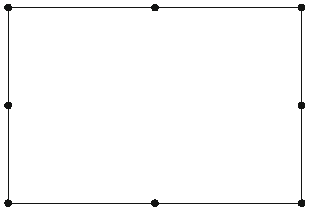
\includegraphics[width=0.86\linewidth]{figures/Chapter_03/Fig_3_06__PDFp111__Bookp099.pdf}
  \captionof{figure}{$Q_2^{(8)}$ 有限元.}\label{fig:taylor-hood-q2-8}
\end{elegantfigure}

Taylor--Hood 有限元空间对是不可压缩流方程离散中最常用的空间对之一,尤其是 $k=2$ 的情形.其广泛应用的一个原因是,与其他满足 inf-sup 条件的有限元空间对相比,$P_2/P_1$ 和 $Q_2/Q_1$ 的实现相对简单.注意,$P_1/P_0$ 和 $Q_1/Q_0$ 空间对已被证明不满足 inf-sup 条件,见例题\hyperref[ex:p1-p0-instability]{3.70} 和例题\hyperref[ex:q1-q0-instability]{3.71}.
\index{Taylor--Hood 有限元}

\end{note}

\begin{note}[Taylor--Hood 有限元的历史评述]\label{note:taylor-hood-history}
由于 Taylor--Hood 有限元空间对广受欢迎,早期已有不少工作试图证明其满足离散 inf-sup 条件.

\textcite{BercovierPironneau1979} 曾用不恰当的范数证明二维 $P_2/P_1$ 空间对满足如下离散 inf-sup 条件:
\begin{equation}\label{eq:taylor-hood-wrong-norm-infsup}
  \sup_{v^h\in V^h\setminus\{0\}}
      \frac{b(v^h,q^h)}{\|v^h\|_{L^2(\Omega)}}
  \ge C\|\nabla q^h\|_{L^2(\Omega)}
  \qquad\forall q^h\in Q^h.
\end{equation}
条件\cref{eq:taylor-hood-wrong-norm-infsup} 与离散 inf-sup 条件\cref{eq:discrete-infsup-condition} 的联系由 \textcite{GuzmanSalgadoSayas2013} 研究.

\textcite{BercovierPironneau1979} 的证明利用了一个估计:压力梯度的平方可由三角形内部边上的导数平方和估计,见该文估计式(2.11).这一估计要求每个三角形至少有两条内部边,因此当时假设每个三角形都含有一个不在边界 $\partial\Omega$ 上的顶点.\textcite{Verfurth1984} 以\cref{eq:taylor-hood-wrong-norm-infsup} 为基础,并利用定理\hyperref[thm:verfurth-continuous-pressure]{3.94} 中的判据,证明了正确的离散 inf-sup 条件\cref{eq:discrete-infsup-condition};其假设仍要求每个三角形至少有一个内部顶点.

随后,\textcite{Stenberg1990} 以及 \textcite{BrezziFalk1991} 证明了二维 $P_3/P_2$ 空间对满足离散 inf-sup 条件.Brezzi 和 Falk 的分析仍对有两条边位于区域边界上的三角形作了一个较弱的假设.最后,\textcite{Boffi1994} 给出了任意阶 $P_k/P_{k-1}$($k\ge2$)空间对的证明,不再对有两条边位于边界上的三角形作限制;该证明同样使用定理\hyperref[thm:verfurth-continuous-pressure]{3.94}.\textcite{MardalSchoberlWinther2013} 为二维 $P_2/P_1$ 空间对构造了 Fortin 算子.

三维 $P_2/P_1$ 空间对满足 inf-sup 条件的证明由 \textcite{Stenberg1987} 给出,随后 \textcite{Boffi1997} 将分析推广到高阶 Taylor--Hood 空间对.该分析要求每个四面体至少有一个顶点位于区域 $\Omega$ 内部.本节的叙述依据 \textcite[第 8.8.2 节]{Boffi2013} 和 \textcite{Boffi1994}.
\index{Taylor--Hood 有限元!历史}
\end{note}

\begin{lemma}[二维情形:三角剖分的必要条件]\label{lem:taylor-hood-two-triangles}
设 $\Omega\subset\mathbb{R}^2$ 是多边形区域,$\{\mathcal{T}^h\}$ 是由三角形构成的正则剖分族.若剖分中的三角形少于三个,则 $P_k/P_{k-1}$($k\ge2$)空间对不满足离散 inf-sup 条件\cref{eq:discrete-infsup-condition}.
\end{lemma}

\begin{proof}
分别讨论 $\mathcal{T}^h$ 由一个三角形和两个三角形组成的情形.

\textbf{$\mathcal{T}^h$ 由一个三角形组成.}由引理\ref{lem:inf-sup-condition},离散 inf-sup 条件等价于
\[
  \nabla\cdot V^h=Q^h,
\]
而这一等式又等价于以下两个包含关系同时成立:
\[
  \nabla\cdot V^h\subset Q^h,
  \qquad Q^h\subset\nabla\cdot V^h.
\]
先考虑参考单元 $\widehat K$,并设其顶点 $0$ 位于原点.在该顶点,$v^h\in V^h$ 的所有导数都由 $V^h$ 的齐次边界条件决定,因而均为零,特别是 $\nabla\cdot v^h(0)=0$.然而,任意 $q^h\in Q^h$ 在 $0$ 点的值不一定为零.因此,$Q^h\not\subset\nabla\cdot V^h$.

对一般网格单元 $K$,设顶点 $a_1$ 映到原点.由变换公式\hyperref[eq:appendix-b-27]{B.27} 或\hyperref[eq:appendix-b-31]{B.31} 可知
\[
  (\nabla\cdot v^h)(a_1)
  =\bigl(DF_K^{-1}(F_K(0))\bigr)^T
       :D_{\widehat x}\widehat v^h(0)=0,
\]
因为 $\widehat v^h$ 在原点的所有导数都为零.由同样的论证可得 $Q^h\not\subset\nabla\cdot V^h$.

\textbf{$\mathcal{T}^h$ 由两个三角形组成.}考虑\cref{fig:taylor-hood-two-triangles} 所示的情形.利用适当的仿射映射,可将一般情形中的 $K_1$ 和 $K_2$ 映到图示构形.为简化记号,仍将这两个三角形记作 $K_1$、$K_2$,并令 $\Omega=K_1\cup K_2$.

\begin{elegantfigure}[0.68\linewidth]
  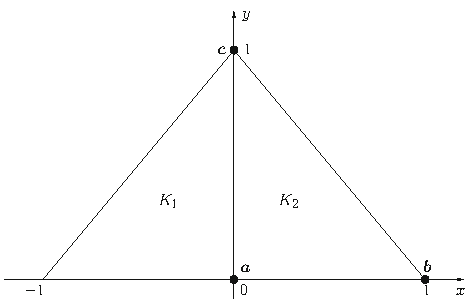
\includegraphics[width=0.90\linewidth]{figures/Chapter_03/Fig_3_07__PDFp112__Bookp100.pdf}
  \captionof{figure}{引理\ref{lem:taylor-hood-two-triangles} 的证明:两个三角形的情形.}\label{fig:taylor-hood-two-triangles}
\end{elegantfigure}

重心坐标见定义\hyperref[def:appendix-b-31]{B.31}.在图示坐标下,它们为
\begin{equation}\label{eq:taylor-hood-two-triangle-barycentric}
\begin{aligned}
  \lambda_{1,a}&=1+x-y, &\lambda_{1,c}&=y,\\
  \lambda_{2,a}&=1-x-y, &\lambda_{2,b}&=x, &\lambda_{2,c}&=y.
\end{aligned}
\end{equation}

令 $L(x)$ 为区间 $(0,1)$ 上关于权函数 $x(1-x)^3$ 的 $k-2$ 次 Legendre 多项式,也就是说,对所有次数 $l<k-2$ 的多项式 $p_l(x)$,有
\begin{equation}\label{eq:taylor-hood-weighted-orthogonality}
  \int_0^1x(1-x)^3L(x)p_l(x)\,\mathrm{d}x=0.
\end{equation}
利用 $L(x)$ 定义一个不依赖于 $y$ 的压力函数,并选取加法常数使其属于 $Q^h$,令其满足
\begin{equation}\label{eq:taylor-hood-pressure-derivative}
  \partial_xq^h(x)=
  \begin{cases}
    -L(-x),&x<0,\\
    L(x),&x\ge0.
  \end{cases}
\end{equation}
下面证明,这个压力函数在 $L^2(\Omega)$ 中正交于 $\nabla\cdot V^h$.

考察离散 inf-sup 条件\cref{eq:discrete-infsup-condition} 中的分子,并作分部积分,可得
\begin{equation}\label{eq:taylor-hood-orthogonality-integration}
  (\nabla\cdot v^h,q^h)
  =-(v^h,\nabla q^h)
  =-\int_{K_1\cup K_2}
       (v_1^h\partial_xq^h)(x)\,\mathrm{d}x.
\end{equation}
因此,只需考虑 $v^h$ 的第一个分量 $v_1^h$.由于 $v_1^h$ 属于 Taylor--Hood 空间,它满足以下性质:
\begin{itemize}
\item $v_1^h$ 在每个网格单元上都是 $k$ 次多项式.
\item 除了公共边以外,$v_1^h$ 在 $K_1$ 和 $K_2$ 的所有边上都为零.对每个网格单元,可将任意一个 $k-2$ 次多项式乘以相应的重心坐标(它们都是一次多项式),从而保证这一性质.
\item $v_1^h$ 在 $x=0$ 处连续.为满足这一性质,可将任意 $k-2$ 次多项式分解为一个关于 $y$ 的任意 $k-2$ 次多项式,以及一个在 $x=0$ 处为零的 $k-2$ 次多项式.
\end{itemize}
由此,$v_1^h$ 的一般形式为
\[
v_1^h(x)=
\begin{cases}
  \lambda_{1,a}\lambda_{1,c}
      \bigl(\widehat p_{k-2}(y)+x\widetilde p_{k-3}(x,y)\bigr),
      &x\in K_1,\\
  \lambda_{2,a}\lambda_{2,c}
      \bigl(\widehat p_{k-2}(y)+xp_{k-3}(x,y)\bigr),
      &x\in K_2,
\end{cases}
\]
其中,下标表示相应多项式的次数.将此表达式代入\cref{eq:taylor-hood-orthogonality-integration}.对 $K_1$ 上的积分使用\cref{eq:taylor-hood-pressure-derivative},作代换 $\xi=-x$,并利用重心坐标\cref{eq:taylor-hood-two-triangle-barycentric} 以及积分上下限的交换,可得
\[
\begin{aligned}
  &-\int_{K_1}\lambda_{1,a}\lambda_{1,c}
       \bigl(\widehat p_{k-2}(y)+x\widetilde p_{k-3}(x,y)\bigr)
       L(-x)\,\mathrm{d}x\\
  &=-\int_{-1}^{0}\int_0^{1+x}
       (1+x-y)y\bigl(\widehat p_{k-2}(y)
                  +x\widetilde p_{k-3}(x,y)\bigr)L(-x)\,\mathrm{d}y\,\mathrm{d}x\\
  &=\int_1^0\int_0^{1-\xi}
       (1-\xi-y)y\bigl(\widehat p_{k-2}(y)
                  -\xi\widetilde p_{k-3}(-\xi,y)\bigr)L(\xi)\,\mathrm{d}y\,\mathrm{d}\xi\\
  &=-\int_{K_2}\lambda_{2,a}\lambda_{2,c}
       \bigl(\widehat p_{k-2}(y)
                  -x\widetilde p_{k-3}(-x,y)\bigr)L(x)\,\mathrm{d}x.
\end{aligned}
\]
将该结果代入\cref{eq:taylor-hood-orthogonality-integration},含 $\widehat p_{k-2}(y)$ 的项相消,得到
\begin{equation}\label{eq:taylor-hood-orthogonality-final}
\begin{aligned}
  (\nabla\cdot v^h,q^h)
  &=-\int_{K_2}\lambda_{2,a}\lambda_{2,b}\lambda_{2,c}
       \bigl(p_{k-3}(x,y)-\widetilde p_{k-3}(-x,y)\bigr)L(x)\,\mathrm{d}x\\
  &=-\int_0^1xL(x)
       \left(\int_0^{1-x}(1-x-y)y\widetilde p_{k-3}(x,y)\,\mathrm{d}y\right)
       \mathrm{d}x.
\end{aligned}
\end{equation}
这里,$\widetilde p_{k-3}(x,y)$ 是一个 $k-3$ 次多项式.直接计算可知,对所有满足 $0\le i+j\le k-3$ 的 $i,j$,
\[
\begin{aligned}
  &\int_0^{1-x}(1-x-y)y x^iy^j\,\mathrm{d}y\\
  &=x^i\frac{(1-x)^{j+3}}{j+2}
       -x^i\frac{(1-x)^{j+3}}{j+3}\\
  &=(1-x)^3\frac{x^i(1-x)^j}{(j+2)(j+3)}\\
  &=(1-x)^3p_{k-3}(x),
\end{aligned}
\]
其中 $p_{k-3}(x)$ 是一个 $k-3$ 次多项式.将此结果代入\cref{eq:taylor-hood-orthogonality-final},再结合\cref{eq:taylor-hood-weighted-orthogonality},得到
\[
  (\nabla\cdot v^h,q^h)
  =-\int_0^1xL(x)(1-x)^3p_{k-3}(x)\,\mathrm{d}x=0.
\]
因此,离散 inf-sup 条件\cref{eq:discrete-infsup-condition} 不可能成立.
\end{proof}

\begin{lemma}[区域分解]\label{lem:domain-decomposition-infsup}
设 $\Omega=\Omega_1\cup\Omega_2$,并令
\[
  V^h(\Omega_i)=\{v^h\in V^h:\ v^h=0\text{ 于 }\Omega\setminus\Omega_i\},
  \qquad i=1,2.
\]
假设在两个子区域上分别成立离散 inf-sup 条件
\[
\begin{aligned}
  \sup_{v^h\in V^h(\Omega_1)\setminus\{0\}}
  \frac{\displaystyle\int_{\Omega_1}(\nabla\cdot v^h)q^h\,\mathrm{d}x}
       {\|\nabla v^h\|_{L^2(\Omega_1)}}
  \ge \beta_{1h}\|q^h\|_{L^2(\Omega_1)}
  \quad\forall q^h\in Q^h,\\
  \sup_{v^h\in V^h(\Omega_2)\setminus\{0\}}
  \frac{\displaystyle\int_{\Omega_2}(\nabla\cdot v^h)q^h\,\mathrm{d}x}
       {\|\nabla v^h\|_{L^2(\Omega_2)}}
  \ge \beta_{2h}\|q^h\|_{L^2(\Omega_2)}
  \quad\forall q^h\in Q^h.
\end{aligned}
\]
则整体区域上成立离散 inf-sup 条件
\begin{equation}\label{eq:domain-decomposition-global-infsup}
  \sup_{v^h\in V^h\setminus\{0\}}
  \frac{(\nabla\cdot v^h,q^h)}{\|\nabla v^h\|_{L^2(\Omega)}}
  \ge \beta_{\mathrm{ish}}\|q^h\|_{L^2(\Omega)}
  \qquad\forall q^h\in Q^h,
\end{equation}
其中 $\beta_{\mathrm{ish}}=\min\{\beta_{1h},\beta_{2h}\}/2$.若 $\Omega_1$ 与 $\Omega_2$ 不相交,则 $\beta_{\mathrm{ish}}=\min\{\beta_{1h},\beta_{2h}\}$.
\end{lemma}

\begin{proof}
任取 $q^h\in Q^h$.由子区域上的 inf-sup 条件以及引理\ref{lem:inf-sup-condition} 中的论证,可分别找到 $v_1^h\in V^h(\Omega_1)$ 和 $v_2^h\in V^h(\Omega_2)$,使得
\begin{equation}\label{eq:domain-decomposition-local-velocities}
\begin{aligned}
  \int_{\Omega_i}(\nabla\cdot v_i^h)q^h\,\mathrm{d}x
  &=\|q^h\|_{L^2(\Omega_i)}^2,\\
  \|\nabla v_i^h\|_{L^2(\Omega_i)}
  &\le \beta_{ih}^{-1}\|q^h\|_{L^2(\Omega_i)},
  \qquad i=1,2.
\end{aligned}
\end{equation}
令 $v^h=v_1^h+v_2^h\in V^h$.由\cref{eq:domain-decomposition-local-velocities} 第一式,
\begin{equation}\label{eq:domain-decomposition-numerator}
\begin{aligned}
  (\nabla\cdot v^h,q^h)
  &=\int_{\Omega_1}(\nabla\cdot v_1^h)q^h\,\mathrm{d}x
    +\int_{\Omega_2}(\nabla\cdot v_2^h)q^h\,\mathrm{d}x\\
  &=\|q^h\|_{L^2(\Omega_1)}^2+\|q^h\|_{L^2(\Omega_2)}^2
    \ge \|q^h\|_{L^2(\Omega)}^2.
\end{aligned}
\end{equation}
利用三角不等式、\cref{eq:domain-decomposition-local-velocities} 第二式,以及子区域上的压力范数不大于整体区域上的范数,得到
\begin{equation}\label{eq:domain-decomposition-gradient-bound}
\begin{aligned}
  \|\nabla v^h\|_{L^2(\Omega)}
  &\le \|\nabla v_1^h\|_{L^2(\Omega_1)}
       +\|\nabla v_2^h\|_{L^2(\Omega_2)}\\
  &\le \beta_{1h}^{-1}\|q^h\|_{L^2(\Omega_1)}
       +\beta_{2h}^{-1}\|q^h\|_{L^2(\Omega_2)}\\
  &\le \max\left\{\frac{1}{\beta_{1h}},\frac{1}{\beta_{2h}}\right\}
       \left(\|q^h\|_{L^2(\Omega_1)}+\|q^h\|_{L^2(\Omega_2)}\right)\\
  &\le \frac{2}{\min\{\beta_{1h},\beta_{2h}\}}
       \|q^h\|_{L^2(\Omega)}.
\end{aligned}
\end{equation}
将\cref{eq:domain-decomposition-numerator,eq:domain-decomposition-gradient-bound} 合并可知,对每个 $q^h\in Q^h$,都存在 $v^h\in V^h$ 使得
\begin{equation}\label{eq:domain-decomposition-ratio}
  \frac{(\nabla\cdot v^h,q^h)}{\|\nabla v^h\|_{L^2(\Omega)}}
  \ge \frac{1}{2}\min\{\beta_{1h},\beta_{2h}\}
       \|q^h\|_{L^2(\Omega)}.
\end{equation}
对\cref{eq:domain-decomposition-ratio} 两边关于 $V^h$ 取上确界,即得\cref{eq:domain-decomposition-global-infsup}.

若两个子区域不相交,则梯度范数的平方满足
\[
\begin{aligned}
  \|\nabla v^h\|_{L^2(\Omega)}^2
  &=\|\nabla v_1^h\|_{L^2(\Omega_1)}^2
    +\|\nabla v_2^h\|_{L^2(\Omega_2)}^2\\
  &\le \beta_{1h}^{-2}\|q^h\|_{L^2(\Omega_1)}^2
       +\beta_{2h}^{-2}\|q^h\|_{L^2(\Omega_2)}^2\\
  &\le \max\{\beta_{1h}^{-2},\beta_{2h}^{-2}\}
       \left(\|q^h\|_{L^2(\Omega_1)}^2
             +\|q^h\|_{L^2(\Omega_2)}^2\right)\\
  &= \min\{\beta_{1h},\beta_{2h}\}^{-2}
       \|q^h\|_{L^2(\Omega)}^2.
\end{aligned}
\]
取平方根,再按上述推理即可得到引理的最后一个结论.
\end{proof}

\begin{note}[子区域多于两个时]\label{note:domain-decomposition-many-subdomains}
若将 $\Omega$ 分解为两个以上的子区域,也可证明与\hyperref[lem:domain-decomposition-infsup]{引理~\ref{lem:domain-decomposition-infsup}} 类似的结论.估计\cref{eq:domain-decomposition-numerator} 的推导不变;在估计\cref{eq:domain-decomposition-gradient-bound} 中,会出现一个较大的因子,该因子取决于子区域相互重叠的次数.因此,相应整体 inf-sup 条件中的常数会较小.

证明 Taylor--Hood 空间对 $P_k/P_{k-1}$($k\ge2$)满足离散 inf-sup 条件时,首先将三角剖分分解为由三个相邻三角形组成的宏单元.\textcite[第 499 页]{Boffi2013} 指出,每个多边形区域的三角剖分都可以表示为若干互不相交的三角形三元组,以及若干个由三元组并成、且至多有三处相交的多边形的并.因此,对估计\cref{eq:domain-decomposition-gradient-bound} 中常数有影响的最大重叠数与剖分无关,整体 inf-sup 常数的缩放因子也就与剖分无关.
\index{Taylor--Hood 有限元!宏单元分解}
\end{note}

\begin{theorem}[二维情形:剖分的充分条件]\label{thm:taylor-hood-2d-sufficient}
设 $\Omega\subset\mathbb{R}^2$ 是多边形区域,$\{\mathcal{T}^h\}$ 是由三角形构成的正则剖分族.若剖分至少含有三个三角形,则 $P_k/P_{k-1}$($k\ge2$)空间对满足离散 inf-sup 条件\cref{eq:discrete-infsup-condition}.
\end{theorem}

\begin{proof}
取准一致剖分族中的任意一个剖分 $\mathcal{T}^h$.由\hyperref[lem:domain-decomposition-infsup]{引理~\ref{lem:domain-decomposition-infsup}} 和\cref{note:domain-decomposition-many-subdomains},只需证明任意一组三个三角形上的离散 inf-sup 条件.

取 $\mathcal{T}^h$ 中任意一个三角形 $K_2$,令其相邻三角形为 $K_1$ 和 $K_3$.通过参考映射 $F_{K_2}^{-1}$ 将三角形映射,使 $K_2$ 成为参考三角形,见\cref{fig:taylor-hood-three-triangles}.为简化记号,仍以 $K_1,K_2,K_3$ 表示映射后的三角形,并令 $\Omega=K_1\cup K_2\cup K_3$.

\begin{elegantfigure}[0.9\linewidth]
  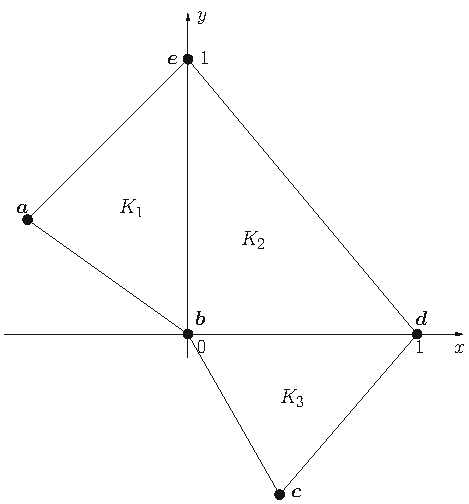
\includegraphics[width=0.9\linewidth]{figures/Chapter_03/Fig_3_08__PDFp117__Bookp105.pdf}
  \captionof{figure}{定理\ref{thm:taylor-hood-2d-sufficient} 的证明:三个三角形的构形.}\label{fig:taylor-hood-three-triangles}
\end{elegantfigure}

证明 $V^h=V^h(\Omega)$ 与 $Q^h=Q^h(\Omega)$ 满足离散 inf-sup 条件的主要思路,是应用\thmref{thm:verfurth-continuous-pressure} 中的判据.为此,只需验证\corref{cor:continuous-pressure-gradient-infsup} 给出的条件.证明采用归纳法,从 $k=2$ 开始.

\textbf{预备工作.}在网格单元 $K_1$ 上,记在边 $E_{a,b}$ 上为零的重心坐标为 $\lambda_{1,a,b}$,其他重心坐标也作类似记号.令 $L_{1,l,x}(x)$ 表示区间 $[x_a,0]$ 上关于测度 $\mathrm{d}\mu_{1,x}$ 的 $l$ 次 Legendre 多项式,其中 $x_a$ 是顶点 $a$ 的 $x$ 坐标,测度定义为
\[
\begin{aligned}
  \int_{x_a}^{0} f(x)\,\mathrm{d}\mu_{1,x}
  &=\int_{K_1}\lambda_{1,a,b}(x,y)\lambda_{1,a,e}(x,y)f(x)
       \,\mathrm{d}x\,\mathrm{d}y,\\
  &\qquad \forall f:[x_a,0]\to\mathbb{R}.
\end{aligned}
\]
该 Legendre 多项式满足
\begin{equation}\label{eq:taylor-hood-legendre-orthogonality}
\begin{aligned}
  0&=\int_{x_a}^{0}L_{1,l,x}(x)p_k(x)\,\mathrm{d}\mu_{1,x}\\
   &=\int_{K_1}\lambda_{1,a,b}\lambda_{1,a,e}
       L_{1,l,x}(x)p_k(x)\,\mathrm{d}x\,\mathrm{d}y,\\
  &\qquad \forall p_k\text{ 且 }\deg p_k<l.
\end{aligned}
\end{equation}
类似地,定义 $L_{2,l,x}(x)$(使用 $\lambda_{2,d,e},\lambda_{2,b,d}$)、$L_{2,l,y}(y)$(使用 $\lambda_{2,d,e},\lambda_{2,b,e}$)以及 $L_{3,l,y}(y)$(使用 $\lambda_{3,b,c},\lambda_{3,c,d}$).所有 Legendre 多项式均作归一化,使其在自变量为 $0$ 时取值为 $1$.

\textbf{归纳起始:$k=2$ 的情形.}任取 $q^h\in Q^h$,逐个三角形定义函数 $v^h=((v_1^h),(v_2^h))^T$:
\[
v_1^h(x,y)=
\begin{cases}
 -\lambda_{1,a,b}\lambda_{1,a,e}\|\nabla q^h\|_{L^2(\Omega)}\sigma,&(x,y)\in K_1,\\
 \begin{aligned}
  -\lambda_{2,d,e}\lambda_{2,b,d}\|\nabla q^h\|_{L^2(\Omega)}\sigma\\[-.25em]
  -\lambda_{2,d,e}\lambda_{2,b,e}\partial_xq^h,
 \end{aligned}&(x,y)\in K_2,\\
 -\lambda_{3,b,c}\lambda_{3,c,d}\partial_xq^h,&(x,y)\in K_3,
\end{cases}
\]
\[
v_2^h(x,y)=
\begin{cases}
 -\lambda_{1,a,b}\lambda_{1,a,e}\partial_yq^h,&(x,y)\in K_1,\\
 \begin{aligned}
  -\lambda_{2,d,e}\lambda_{2,b,e}\|\nabla q^h\|_{L^2(\Omega)}\tau\\[-.25em]
  -\lambda_{2,d,e}\lambda_{2,b,d}\partial_yq^h,
 \end{aligned}&(x,y)\in K_2,\\
 -\lambda_{3,b,c}\lambda_{3,c,d}\|\nabla q^h\|_{L^2(\Omega)}\tau,&(x,y)\in K_3.
\end{cases}
\]
选取 $\sigma,\tau\in\{-1,1\}$,使得下列量非负:
\[
\begin{aligned}
  \sigma_1&=\sigma\|\nabla q^h\|_{L^2(\Omega)}\Bigl(
       \int_{K_1}\lambda_{1,a,b}\lambda_{1,a,e}\partial_xq^h\,\mathrm{d}x\\
       &\qquad+\int_{K_2}\lambda_{2,d,e}\lambda_{2,b,d}\partial_xq^h\,\mathrm{d}x\Bigr),\\
  \tau_1&=\tau\|\nabla q^h\|_{L^2(\Omega)}\Bigl(
       \int_{K_2}\lambda_{2,d,e}\lambda_{2,b,e}\partial_yq^h\,\mathrm{d}x\\
       &\qquad+\int_{K_3}\lambda_{3,b,c}\lambda_{3,c,d}\partial_yq^h\,\mathrm{d}x\Bigr).
\end{aligned}
\]

下面验证 $v^h\in V^h$.首先,在每个网格单元上,$v^h$ 的每一项都是两个重心坐标(一次多项式)与常数因子的乘积,因此 $v^h$ 在各网格单元上至多为二次多项式.其次,由于定义中包含在 $\partial\Omega$ 上为零的相应重心坐标,$v^h$ 在 $\partial\Omega$ 上为零.最后,$v^h$ 在边 $E_{b,e}$ 和 $E_{b,d}$ 上连续.以 $E_{b,e}$ 为例,在该边上有 $\lambda_{1,a,e}=\lambda_{2,d,e}$、$\lambda_{1,a,b}=\lambda_{2,b,d}$;此外,$q^h$ 连续,故其切向导数 $\partial_xq^h$ 也连续.因此 $v^h$ 在 $E_{b,e}$ 上连续.对 $E_{b,d}$ 可作类似论证.

现在证明\cref{eq:continuous-pressure-gradient-test} 中关于速度范数的相应估计.利用重心坐标的取值均在 $[0,1]$ 内以及三角不等式,得到
\begin{equation}\label{eq:taylor-hood-k2-velocity-bound}
\begin{aligned}
  \|v^h\|_{L^2(\Omega)}^2
  &=\int_{K_1}\bigl((v_1^h)^2+(v_2^h)^2\bigr)\,\mathrm{d}x\\
  &\quad+\int_{K_2}\bigl((v_1^h)^2+(v_2^h)^2\bigr)\,\mathrm{d}x\\
  &\quad+\int_{K_3}\bigl((v_1^h)^2+(v_2^h)^2\bigr)\,\mathrm{d}x\\
  &\le \int_{K_1}\left(\|\nabla q^h\|_{L^2(\Omega)}^2
                        +(\partial_yq^h)^2\right)\,\mathrm{d}x\\
  &\quad+2\int_{K_2}\left(2\|\nabla q^h\|_{L^2(\Omega)}^2
                        +(\partial_xq^h)^2+(\partial_yq^h)^2\right)\,\mathrm{d}x\\
  &\quad+\int_{K_3}\left((\partial_xq^h)^2
                        +\|\nabla q^h\|_{L^2(\Omega)}^2\right)\,\mathrm{d}x\\
  &\le C\Bigl(|\Omega|\|\nabla q^h\|_{L^2(\Omega)}^2
       +\|\nabla q^h\|_{L^2(K_1)}^2+\|\nabla q^h\|_{L^2(K_2)}^2\\
       &\qquad+\|\nabla q^h\|_{L^2(K_3)}^2\Bigr)\\
  &\le C_2\|\nabla q^h\|_{L^2(\Omega)}^2.
\end{aligned}
\end{equation}
由此可见,常数 $C_2$ 与 $q^h$ 和 $v^h$ 均无关.

为证\cref{eq:continuous-pressure-gradient-test} 中关于双线性型的另一个不等式,先证明若 $b(v^h,q^h)=0$,则 $\nabla q^h=0$.直接计算可得
\begin{equation}\label{eq:taylor-hood-k2-kernel-identity}
\begin{aligned}
  0=-b(v^h,q^h)
  &=\int_\Omega(\nabla\cdot v^h)q^h\,\mathrm{d}x
   =-\int_\Omega v^h\cdot\nabla q^h\,\mathrm{d}x\\
  &=\int_{K_1}\lambda_{1,a,b}\lambda_{1,a,e}(\partial_yq^h)^2\,\mathrm{d}x+\sigma_1\\
  &\quad+\int_{K_2}\lambda_{2,d,e}\lambda_{2,b,e}(\partial_xq^h)^2\,\mathrm{d}x\\
  &\quad+\int_{K_2}\lambda_{2,d,e}\lambda_{2,b,d}(\partial_yq^h)^2\,\mathrm{d}x\\
  &\quad+\tau_1+\int_{K_3}\lambda_{3,b,c}\lambda_{3,c,d}(\partial_xq^h)^2\,\mathrm{d}x.
\end{aligned}
\end{equation}
由于重心坐标在网格单元内部为正,且 $\sigma_1,\tau_1$ 均非负,上式中的每一项都必须为零.因此,立即得到 $\partial_yq^h=0$ 于 $K_1$,$\partial_xq^h=\partial_yq^h=0$ 于 $K_2$,以及 $\partial_xq^h=0$ 于 $K_3$.再由 $\sigma_1=0$ 及 $\partial_xq^h=0$ 于 $K_2$,可得 $\partial_xq^h=0$ 于 $K_1$;同理可得 $\partial_yq^h=0$ 于 $K_3$.综上,$\nabla q^h=0$ 于 $\Omega$,故存在常数 $C_1(q^h)>0$,使得
\[
  -b(v^h,q^h)\ge C_1(q^h)\|\nabla q^h\|_{L^2(\Omega)}^2.
\]
将 $v^h$ 换为 $-v^h$,便得到\cref{eq:continuous-pressure-gradient-test} 所需的双线性型下界.
还需证明可选取一个与 $q^h$ 无关的正数 $C_1$.首先注意,对任意 $\alpha\in\mathbb{R}\setminus\{0\}$,将函数换成 $\alpha q^h$ 并相应地将速度换成 $\alpha v^h$,所得估计中的常数仍为 $C_1(q^h)$.因此,$C_1(q^h)$ 在球面
\[
  S_q=\{q^h\in Q^h:\ \|q^h\|_{L^2(\Omega)}=q>0\}
\]
上取遍所有可能的值.由于 $Q^h$ 是有限维空间,$S_q$ 是紧集.

另一方面,任取固定的 $\widetilde q^h\in Q^h$,考虑 $q_\varepsilon^h=q^h+\varepsilon\widetilde q^h$,并以同样方式定义 $v_\varepsilon^h$,即可得到常数 $C_1(q_\varepsilon^h)$.当 $\varepsilon\to0$ 时,$q_\varepsilon^h\to q^h$;由范数的连续性以及微分的线性性,$v_\varepsilon^h\to v^h$.由积分的线性性和范数的连续性可知
\[
\begin{aligned}
\lim_{\varepsilon\to0}
  \frac{-b(v_\varepsilon^h,q_\varepsilon^h)}
       {\|\nabla q_\varepsilon^h\|_{L^2(\Omega)}^2}
 &=\lim_{\varepsilon\to0}
  \frac{-\int_\Omega v_\varepsilon^h\cdot\nabla q^h\,\mathrm{d}x}
       {\|\nabla q_\varepsilon^h\|_{L^2(\Omega)}^2}\\
 &\quad-\lim_{\varepsilon\to0}
  \frac{\varepsilon\int_\Omega v_\varepsilon^h\cdot\nabla\widetilde q^h\,\mathrm{d}x}
       {\|\nabla q_\varepsilon^h\|_{L^2(\Omega)}^2}\\
 &=\frac{-\int_\Omega v^h\cdot\nabla q^h\,\mathrm{d}x}
       {\|\nabla q^h\|_{L^2(\Omega)}^2}
 \ge C_1(q^h).
\end{aligned}
\]
因此可令 $C_1(q_\varepsilon^h)\to C_1(q^h)$,从而可将 $C_1(q^h)$ 选为关于 $q^h$ 连续的函数.由于 $C_1(q^h)$ 在 $S_q$ 上连续,且 $S_q$ 紧,由 Weierstrass 定理可知 $C_1(q^h)$ 能取到其下确界,且下确界就是其最小值.由于 $C_1(q^h)$ 的取值均为正数,故
\[
  C_1=\inf_{q^h\in S_q}C_1(q^h)
     =\min_{q^h\in S_q}C_1(q^h)>0
\]
是满足\cref{eq:continuous-pressure-gradient-test} 第一条不等式的正数,且与 $q^h$ 无关.

以上分析是在\cref{fig:taylor-hood-three-triangles} 所示的参考构形上进行的,因此 $C_1$ 与网格尺度无关.将该构形变换到区域 $\Omega$ 中,需要分别变换离散 inf-sup 条件的分子和分母.变换分子会产生因子 $|\det(B_K)|^{-1}$,其中 $B_K$ 是仿射变换的矩阵,见\hyperref[eq:appendix-b-35]{B.35}.分母中的两个范数各产生因子 $|\det(B_K)|^{-1/2}$,见\hyperref[eq:appendix-b-32]{B.32} 和\hyperref[eq:appendix-b-34]{B.34}.因此这些因子相消,$\Omega$ 中该构形的 inf-sup 常数与网格尺度无关.

\textbf{归纳步骤:$k>2$ 的情形.}归纳假设:\thmref{thm:taylor-hood-2d-sufficient} 对 $P_{k-1}/P_{k-2}$ 已成立.再次任取 $q^h\in Q^h$.假设至少有一个三角形上 $q^h$ 的次数恰为 $k-1$;否则,结论由归纳假设直接得到.按 $k=2$ 时的相同思路定义相应的 $v^h$:
\[
v_1^h(x,y)=
\begin{cases}
 -\lambda_{1,a,b}\lambda_{1,a,e}\|\nabla q^h\|_{L^2(\Omega)}L_{1,k-2,x}(x)\sigma,&(x,y)\in K_1,\\
 \begin{aligned}
  -\lambda_{2,d,e}\lambda_{2,b,d}\|\nabla q^h\|_{L^2(\Omega)}L_{2,k-2,x}(x)\sigma\\[-.25em]
  -\lambda_{2,d,e}\lambda_{2,b,e}\partial_xq^h,
 \end{aligned}&(x,y)\in K_2,\\
 -\lambda_{3,b,c}\lambda_{3,c,d}\partial_xq^h,&(x,y)\in K_3,
\end{cases}
\]
\[
v_2^h(x,y)=
\begin{cases}
 -\lambda_{1,a,b}\lambda_{1,a,e}\partial_yq^h,&(x,y)\in K_1,\\
 \begin{aligned}
  -\lambda_{2,d,e}\lambda_{2,b,e}\|\nabla q^h\|_{L^2(\Omega)}L_{2,k-2,y}(y)\tau\\[-.25em]
  -\lambda_{2,d,e}\lambda_{2,b,d}\partial_yq^h,
 \end{aligned}&(x,y)\in K_2,\\
 -\lambda_{3,b,c}\lambda_{3,c,d}\|\nabla q^h\|_{L^2(\Omega)}L_{3,k-2,y}(y)\tau,&(x,y)\in K_3.
\end{cases}
\]
选取 $\sigma,\tau\in\{-1,1\}$,使得下列两项非负:
\[
\begin{aligned}
  \sigma_1&=\sigma\|\nabla q^h\|_{L^2(\Omega)}\Bigl(
       \int_{K_1}\lambda_{1,a,b}\lambda_{1,a,e}L_{1,k-2,x}\partial_xq^h\,\mathrm{d}x\\
       &\qquad+\int_{K_2}\lambda_{2,d,e}\lambda_{2,b,d}L_{2,k-2,x}\partial_xq^h\,\mathrm{d}x\Bigr),\\
  \tau_1&=\tau\|\nabla q^h\|_{L^2(\Omega)}\Bigl(
       \int_{K_2}\lambda_{2,d,e}\lambda_{2,b,e}L_{2,k-2,y}\partial_yq^h\,\mathrm{d}x\\
       &\qquad+\int_{K_3}\lambda_{3,b,c}\lambda_{3,c,d}L_{3,k-2,y}\partial_yq^h\,\mathrm{d}x\Bigr).
\end{aligned}
\]
利用与 $k=2$ 情形相同的论证,可以证明 $v^h\in V^h$.还需补充两点:其一,Legendre 多项式的次数为 $k-2$,重心坐标的次数为 $1$,所以 $v^h$ 在每个网格单元上的次数至多为 $k$;其二,由归一化方式可知,$L_{1,k-2,x}$ 与 $L_{2,k-2,x}$ 在 $x=0$ 处取值相同,$L_{2,k-2,y}$ 与 $L_{3,k-2,y}$ 在 $y=0$ 处取值相同,这保证了 $v^h$ 的连续性.

证明\cref{eq:continuous-pressure-gradient-test} 中第二个估计的方式与\cref{eq:taylor-hood-k2-velocity-bound} 相同;此外只需用到 Legendre 多项式有界,且这些界与 $q^h,v^h$ 无关.现在假设 $b(v^h,q^h)=0$.作与\cref{eq:taylor-hood-k2-kernel-identity} 类似的计算,并使用 $k=2$ 时相同的论证,可得 $\partial_yq^h=0$ 于 $K_1$,$\partial_xq^h=\partial_yq^h=0$ 于 $K_2$,$\partial_xq^h=0$ 于 $K_3$,且 $\sigma_1=\tau_1=0$.由 $\sigma_1=0$ 以及 $\partial_xq^h=0$ 于 $K_2$,得到
\[
  \int_{K_1}\lambda_{1,a,b}\lambda_{1,a,e}
       L_{1,k-2,x}(x)\partial_xq^h\,\mathrm{d}x=0.
\]
由正交性\cref{eq:taylor-hood-legendre-orthogonality} 可知,$\partial_xq^h$ 在 $K_1$ 上是次数小于 $k-2$ 的多项式.因此,$q^h$ 在 $K_1$ 上的次数小于 $k-1$.同理,$q^h$ 在 $K_3$ 上的次数也小于 $k-1$.综上,$q^h$ 在每个网格单元上的次数均小于 $k-1$,这与假设矛盾.因此存在常数 $C_1(q^h)>0$,使得
\[
  -b(v^h,q^h)\ge C_1(q^h)\|\nabla q^h\|_{L^2(\Omega)}^2.
\]
同样将 $v^h$ 换为 $-v^h$,即可得到\cref{eq:continuous-pressure-gradient-test} 所需的双线性型下界.
选取与 $q^h$ 及网格尺度无关的 $C_1$ 的论证与 $k=2$ 时相同.至此定理得证.
\end{proof}

\begin{theorem}[三维情形]\label{thm:taylor-hood-3d}
设 $\Omega\subset\mathbb{R}^3$ 是多面体区域,$\{\mathcal{T}^h\}$ 是由四面体构成的正则剖分族.假设每个四面体至少有一个顶点位于 $\Omega$ 内部,则 $P_k/P_{k-1}$($k\ge2$)空间对满足离散 inf-sup 条件\cref{eq:discrete-infsup-condition}.
\end{theorem}

\begin{proof}
证明使用\cref{subsec:macroelement-techniques} 中介绍的宏单元方法.

考虑 $\mathcal{T}^h$ 的一个重叠宏单元划分,并对 $\Omega$ 内部的每个顶点 $a$ 定义宏单元
\[
  M_a=\{K:\ K\in\mathcal{T}^h,\ a\text{ 是 }K\text{ 的顶点}\}.
\]
由于剖分族正则,具有共同顶点的四面体数存在一致上界.因此,宏单元类型只有有限种.由每个四面体至少有一个内部顶点的假设可知,每个四面体至少属于一个宏单元;而每个网格单元至多属于四个宏单元.因此,\hyperref[lem:macroelement-velocity-1]{引理~\ref{lem:macroelement-velocity-1}} 和\cref{note:macroelement-overlap} 的几何假设均成立.剩下只需验证宏单元条件\cref{eq:macroelement-condition}.

任取 $K\in M_a$,并令 $E$ 为 $K$ 的一条以 $a$ 为端点的边.选择坐标系,使 $E$ 位于 $x$ 轴上.任取
\[
  q^h\in Q_{\mathrm{grad},M_a}^h\cap Q_{0,M_a}^h.
\]
先证明 $q^h$ 在 $K$ 上为常数.为此定义函数 $v^h$:对 $M_a$ 中所有与边 $E$ 相邻的网格单元 $K_i$,令
\[
  v^h=\bigl(-\lambda_{i,1}\lambda_{i,2}\partial_xq^h,\ 0,\ 0\bigr)^T
  \quad\text{于 }K_i,
\]
其中,$\lambda_{i,1}$ 和 $\lambda_{i,2}$ 是 $K_i$ 中分别对应于不含公共边 $E$ 的两个面的重心坐标.在 $M_a$ 中其他网格单元上,令 $v^h=0$.下面验证 $v^h\in V_{0,M_a}^h$.首先,$\partial_xq^h$ 是 $k-2$ 次多项式,而 $\lambda_{i,1},\lambda_{i,2}$ 都是一次多项式,所以 $v^h$ 是 $k$ 次多项式.其次,由所选重心坐标的构造可知,$v^h|_{\partial M_a}=0$.最后,由于 $q^h$ 连续,其在各面上的切向导数也连续;边 $E$ 是所有含该边的面上的切向量,故 $\partial_xq^h$ 在这些面上连续.重心坐标在这些面上也连续,而 $v^h$ 在其他面上为零.因此 $v^h$ 连续,确有 $v^h\in V_{0,M_a}^h$.

由于 $q^h\in Q_{\mathrm{grad},M_a}^h$,有
\[
\begin{aligned}
  0&=(\nabla\cdot v^h,q^h)_{M_a}
    =-\int_{M_a}v^h\cdot\nabla q^h\,\mathrm{d}x\\
   &=\sum_{K_i\in M_a:\,K_i\supset E}
       \int_{K_i}\lambda_{i,1}\lambda_{i,2}
              (\partial_xq^h)^2\,\mathrm{d}x.
\end{aligned}
\]
因此 $\partial_xq^h=0$,从而 $q^h$ 在每个这样的 $K_i$ 上都与 $x$ 无关,特别是在 $K$ 上如此.对 $K$ 中以 $a$ 为端点的另外两条边重复上述论证,可知 $q^h$ 在 $K$ 上沿三个线性无关方向的偏导数均为零,故 $\nabla q^h=0$ 于 $K$.

对 $M_a$ 中每个 $K$ 重复上述过程,可知 $q^h$ 在每个网格单元上均为常数.由于 $q^h$ 连续,它在整个 $M_a$ 上为常数.$Q_{0,M_a}^h$ 中唯一的常数函数是零,故 $q^h=0$,这正是宏单元条件\cref{eq:macroelement-condition}.
\end{proof}

\begin{note}[$Q_k/Q_{k-1}$($k\ge2$)空间对]\label{note:qk-qkminus1-stability}
二维情形下 $Q_2/Q_1$ 空间对满足离散 inf-sup 条件\cref{eq:discrete-infsup-condition},由\textcite{Stenberg1984} 使用其文中提出的宏单元方法证明;该宏单元由两个网格单元组成.随后,\textcite{Stenberg1990} 将分析推广到高阶 $Q_k/Q_{k-1}$ 空间对.三维情形下 $Q_2/Q_1$ 空间对的离散 inf-sup 条件由\textcite{Stenberg1987} 证明.
\index{$Q_k/Q_{k-1}$ 空间对}
\end{note}

\begin{note}[修改的 Taylor--Hood 有限元]\label{note:modified-taylor-hood}
设三角剖分 $\mathcal{T}^h$ 由三角形、四边形或六面体构成,并对这些网格单元作正则加密,例如将三角形的各边中点相连,得到剖分 $\mathcal{T}^{h/2}$.

为简明起见,只讨论三角形.修改的 Taylor--Hood 有限元空间取细网格上的 $P_1^{h/2}$ 作为速度空间,取粗网格上的 $P_1^h$ 作为压力空间.细网格 $P_1^{h/2}$ 的自由度数与粗网格空间 $P_2^h$ 相同,但此处采用的是分片线性函数,而非分片二次函数.四边形和六面体也可作类似构造.若已有程序只支持最低阶有限元,这种修改的 Taylor--Hood 空间便可能有用.

修改的 Taylor--Hood 空间对满足离散 inf-sup 条件的性质,例如可用\cref{note:taylor-hood-history} 中提到的 Bercovier--Pironneau(1979)和 Verfürth(1984)的方法证明.
\index{Taylor--Hood 有限元!修改的 Taylor--Hood 有限元}
\end{note}

\subsection{单纯形网格上的不连续压力空间}\label{sec:scott-vogelius}

\begin{note}[动机]\label{note:discontinuous-pressure-motivation}
文献中采用不连续压力有限元空间(finite element spaces with discontinuous pressure)的一个动机,是这类空间具有局部质量守恒(local mass conservation)性质.关于这一点,见笔记\hyperref[note:stokes-local-mass-conservation-discontinuous-pressure]{4.32}.
\index{不连续压力!局部质量守恒}
\end{note}

\begin{note}[构造的基本思路]\label{note:discontinuous-pressure-construction}
在单纯形网格上采用不连续压力逼近的空间对包括:\textcite{CrouzeixRaviart1973} 提出的 $P_2^{\mathrm{bubble}}/P_1^{\mathrm{disc}}$ 空间对;\textcite{ScottVogelius1985} 引入的 Scott--Vogelius 空间对 $P_k/P_{k-1}^{\mathrm{disc}}$($k\ge2$);以及\textcite{BernardiRaugel1985} 提出的 Bernardi--Raugel 空间.例题\hyperref[ex:p1-p0-instability]{3.70} 和\hyperref[ex:scott-vogelius-macroelement]{3.73} 已经说明,采用 $P_k/P_{k-1}^{\mathrm{disc}}$ 组合通常会违反离散 inf-sup 条件\cref{eq:discrete-infsup-condition}.

Scott--Vogelius 有限元仍采用 $P_k/P_{k-1}^{\mathrm{disc}}$($k\ge2$),但只在能够证明离散 inf-sup 条件成立的特殊网格上使用.$P_2^{\mathrm{bubble}}/P_1^{\mathrm{disc}}$ 有限元和 Bernardi--Raugel 有限元的基本思路,则是向离散速度空间加入气泡函数,直至速度空间足够大,从而满足离散 inf-sup 条件;参见笔记\hyperref[note:infsup-not-inherited]{3.52}.
\index{Scott--Vogelius 有限元}
\index{Bernardi--Raugel 有限元}
\end{note}

\begin{note}[Scott--Vogelius 有限元空间对]\label{note:scott-vogelius-pair}
该空间对为 $P_k/P_{k-1}^{\mathrm{disc}}$($k\ge2$).由于
\[
  \nabla\cdot V^h\subseteq \nabla\cdot P_k
      =P_{k-1}^{\mathrm{disc}}=Q^h,
\]
这一空间对中的有限元速度是弱无散的,这是一个理想性质.不过,正如例题\hyperref[ex:scott-vogelius-macroelement]{3.73} 已经说明的,Scott--Vogelius 有限元通常不满足离散 inf-sup 条件\cref{eq:discrete-infsup-condition}.但在某些特殊情形,也就是特殊网格上,可以证明 $P_k/P_{k-1}^{\mathrm{disc}}$ 空间对满足离散 inf-sup 条件.本节将概述已知结果.
\index{Scott--Vogelius 有限元!弱无散性}
\end{note}

\begin{note}[$P_k/P_{k-1}^{\mathrm{disc}}$ 空间对的二维情形]\label{note:scott-vogelius-2d}
\textcite{ScottVogelius1985} 已证明,在二维情形下,只要网格中没有所谓的奇异顶点(singular vertex),$k\ge4$ 时 $P_k/P_{k-1}^{\mathrm{disc}}$ 空间对满足离散 inf-sup 条件\cref{eq:discrete-infsup-condition}.若一个内部顶点处相交的网格边落在两条直线上,就称该顶点为奇异顶点.关于离散 inf-sup 条件普遍成立的反例正是采用了奇异顶点,见\cref{fig:scott-vogelius-macroelement}.

解决这一问题的基本思路是采用不含奇异顶点的网格,为此构造所谓的重心加密网格(barycentric-refined mesh).从任意一个可容许的三角剖分出发,将每个网格单元的所有顶点与该单元的重心相连,即可引入新的网格边.这样便把单元细分为更小的三角形,\cref{fig:barycentric-refinement} 给出了一个例子.\textcite{Qin1994} 证明,在重心加密网格上,$k\in\{2,3\}$ 时 $P_k/P_{k-1}^{\mathrm{disc}}$ 空间对满足离散 inf-sup 条件;$k=2$ 的证明也见例题\hyperref[ex:barycentric-refinement-scott-vogelius]{4.144}.注意,$k\ge4$ 的情形已由\textcite{ScottVogelius1985} 的分析涵盖.

在文献中,重心加密网格上的 $P_2/P_1^{\mathrm{disc}}$ 空间对偶尔会被采用,尤其用于展示具有弱无散速度解的空间对的优点,例如参见 John et al.(2015)及其中的参考文献.
\index{奇异顶点}
\index{重心加密网格}
\end{note}

\begin{note}[$P_k/P_{k-1}^{\mathrm{disc}}$ 空间对的三维情形]\label{note:scott-vogelius-3d}
在三维情形下,采用重心加密网格可以避免奇异顶点和奇异边.\textcite{Zhang2005} 已证明,在这类网格上,$k\le3$ 时 $P_k/P_{k-1}^{\mathrm{disc}}$ 空间对满足离散 inf-sup 条件.证明使用了\textcite{Stenberg1984} 的宏单元方法,即第\hyperref[subsec:macroelement-techniques]{3.5.4 节} 介绍的方法.

\begin{elegantfigure}[0.9\linewidth]
  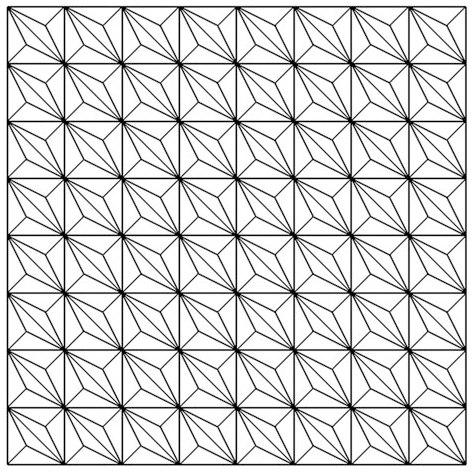
\includegraphics[width=0.78\linewidth]{figures/Chapter_03/Fig_3_09__PDFp125__Bookp113.pdf}
  \captionof{figure}{单位正方形上的单纯形重心加密网格.}\label{fig:barycentric-refinement}
\end{elegantfigure}

在三维重心加密网格上,Scott--Vogelius 空间对 $P_3/P_2^{\mathrm{disc}}$ 曾用于电化学应用,见\textcite{Fuhrmann2009,Fuhrmann2011};也用于湍流模拟,见\textcite{Cuff2015}.
\index{Scott--Vogelius 有限元!三维情形}
\end{note}

\begin{note}[$P_2^{\mathrm{bubble}}/P_1^{\mathrm{disc}}$ 和 $P_3^{\mathrm{bubble}}/P_2^{\mathrm{disc}}$ 空间对]\label{note:bubble-discontinuous-pressure-pairs}
该类空间对由\textcite{CrouzeixRaviart1973} 提出.若要在任意单纯形网格上获得压力为分片线性不连续函数的 inf-sup 稳定空间对,就需要扩充速度空间.事实证明,加入气泡函数,也就是局部函数,便已足够.二维情形下,只需加入所有网格单元的气泡函数;每个三角形单元上的单元气泡函数是三个重心坐标的乘积 $\lambda_1\lambda_2\lambda_3$.

在三维情形下,\textcite{CrouzeixRaviart1973} 提出的扩充由所有单元气泡函数和所有面气泡函数(face bubble functions)组成.对具有重心坐标 $\lambda_1,\ldots,\lambda_4$ 的网格单元 $K$,单元气泡函数为 $\lambda_1\lambda_2\lambda_3\lambda_4$;四个面气泡函数则分别是三个互不相同重心坐标的乘积,例如 $\lambda_1\lambda_2\lambda_3$.因此,每个速度分量有 15 个自由度用于扩充,局部扩充空间的维数为 45.从实际计算角度看,必须考虑到气泡函数是高次多项式,使用它们需要采用高阶求积公式.\textcite[第 553 页]{GreshoSani2000} 认为 $P_2^{\mathrm{bubble}}/P_1^{\mathrm{disc}}$ 空间对是一个很好的选择.

通过气泡函数扩充空间对以获得稳定性的做法可以推广到高阶空间.例如,在\textcite{CrouzeixRaviart1973} 中还给出了二维情形的 $P_3^{\mathrm{bubble}}/P_2^{\mathrm{disc}}$ 空间对.
\index{气泡函数!单元气泡函数}
\index{气泡函数!面气泡函数}
\end{note}

\begin{note}[一阶 Bernardi--Raugel 元 $P_1^{\mathrm{BR}}/P_0^{\mathrm{disc}}$]\label{note:bernardi-raugel-first-order}
构造一阶 Bernardi--Raugel 有限元时,需要在 $P_1(K)$ 空间中加入真正的向量值基函数.设 $\lambda_i$($i=1,\ldots,d+1$)为定义\hyperref[def:appendix-b-31]{B.31} 中的重心坐标.利用这些函数定义面气泡函数(二维时即边气泡函数):
\[
  v_{\mathrm{bub},i}^h
  =\left(\prod_{\substack{j=1\\j\ne i}}^{d+1}\lambda_j\right)n_i,
  \qquad i=1,\ldots,d+1,
\]
其中 $n_i$ 是与顶点 $a_i$ 对面的面 $E_i$ 上的单位外法向量.这些面气泡函数是多项式.局部有限元空间为
\[
  P_1^{\mathrm{BR}}(K)
  =P_1(K)^d\oplus\operatorname{span}\{v_{\mathrm{bub},i}^h:
      i=1,\ldots,d+1\}.
\]
自由度包括顶点处的函数值 $v^h(a_i)$(共 $d(d+1)$ 个数值)以及各面上的通量 $v^h\cdot n_i$(共 $d+1$ 个数值).因此,用于扩充的局部自由度总数为 $(d+1)^2$.

相应的整体速度空间由连续函数构成.两个网格单元 $K_1,K_2$ 在面 $E$ 上相邻时,它们的面气泡函数在 $E$ 上可以组合为连续函数.具体而言,分别使用两个网格单元各自指向外侧的法向量时,面气泡函数在 $E$ 上的迹互为相反数;按此法向量定义的面通量也改变符号,因此 $v_{\mathrm{bub},i}^h|_{K_1}$ 和 $v_{\mathrm{bub},i}^h|_{K_2}$ 前的系数绝对值相同而符号相反.这样,基函数与局部泛函的组合便给出整体连续函数.

整体空间的离散 inf-sup 条件证明基于 Fortin 算子的构造,见\hyperref[lem:fortin-criterion]{引理~\ref{lem:fortin-criterion}}.该算子具有\cref{eq:fortin-operator-construction} 的形式,其中 $P_1^h=P_{\mathrm{Cle}}^h$,另见\cref{note:fortin-detailed-construction}.对每个网格单元 $K$,算子由下列条件定义:
\[
\begin{aligned}
  P_{\mathrm{For}}^h v(a_i)&=P_{\mathrm{Cle}}^h v(a_i),\\
  \int_{E_i}(v-P_{\mathrm{For}}^h v)\cdot n_i\,\mathrm{d}s&=0,
  \qquad i=1,\ldots,d+1.
\end{aligned}
\]
Fortin 判据中的性质\hyperref[eq:fortin-property]{(3.82)} 已由\textcite[引理 II.4]{BernardiRaugel1985} 证明.Bernardi--Raugel 一阶空间对 $P_1^{\mathrm{BR}}/P_0^{\mathrm{disc}}$ 目前只偶尔用于学术研究.
\index{Bernardi--Raugel 有限元!一阶}
\end{note}

\begin{note}[四边形网格单元构成的剖分族]\label{note:bernardi-raugel-quadrilaterals}
\textcite{BernardiRaugel1985} 指出,速度空间的构造及 inf-sup 条件的证明均可推广到由四边形组成的正则剖分族.这一结果曾用于证明四边形网格上不连续压力空间的离散 inf-sup 条件,见笔记\hyperref[note:unmapped-qk-pdisc-2d]{3.143} 和例题\hyperref[ex:unmapped-q2-p1]{3.144}.
\index{Bernardi--Raugel 有限元!四边形网格}
\end{note}

\begin{note}[三维二阶 Bernardi--Raugel 元 $P_2^{\mathrm{BR}}/P_1^{\mathrm{disc}}$]\label{note:bernardi-raugel-second-order-3d}
在四面体网格上,\textcite{BernardiRaugel1985} 提出的局部速度空间为
\[
  P_2^{\mathrm{BR}}(K)
  =P_2(K)^3\oplus\operatorname{span}\{v_{\mathrm{bub},i}^h:
       i=1,\ldots,4\}
       \oplus\bigl(\operatorname{span}\{\lambda_1\lambda_2\lambda_3\lambda_4\}\bigr)^3.
\]
该构造与不连续压力空间配合使用,可视为二维情形下\textcite{CrouzeixRaviart1973} 所引入空间对的推广.$P_2^{\mathrm{BR}}(K)$ 的自由度包括顶点处和边中点处的函数值(来自 $P_2$,共 30 个自由度)、各面上的通量(来自 $\operatorname{span}\{v_{\mathrm{bub},i}^h\}$,共 4 个自由度),以及矩
\[
  \int_K x_i\,\nabla\cdot v^h\,\mathrm{d}x,
  \qquad i=1,2,3.
\]
因此,局部空间的维数为 37.

沿用\cref{note:bernardi-raugel-first-order} 中的相同论证,可知相应的整体速度空间由连续函数组成.通过类似\cref{note:bernardi-raugel-first-order} 所述方式构造 Fortin 算子,可以证明离散 inf-sup 条件\cref{eq:discrete-infsup-condition} 成立.

\textcite{JohnKindlSuciu2010} 给出了 $P_2^{\mathrm{BR}}/P_1^{\mathrm{disc}}$ 空间对的数值模拟.该文选择这一空间对而非 Taylor--Hood 空间对 $P_2/P_1$ 的主要原因,是所用多重网格求解器(见第\hyperref[subsec:multigrid-method]{9.2.2 节})对压力不连续的空间对效率更高.总的来说,据目前所知,这一空间对仍只用于学术研究.
\index{Bernardi--Raugel 有限元!三维二阶}
\end{note}
\subsection{四边形与六面体网格上的不连续压力空间}\label{sec:quadrilateral-discontinuous-pressure}

\begin{note}[$Q_k/P_{k-1}^{\mathrm{disc}}$ 空间对]\label{note:qk-pdisc-mapped-unmapped}
在四边形和六面体网格上,速度协调、压力不连续的常用空间对是 $Q_k/P_{k-1}^{\mathrm{disc}}$,其中 $k\ge2$.例题\hyperref[ex:q1-q0-instability]{3.71} 已说明,$Q_1/P_0^{\mathrm{disc}}=Q_1/Q_0$ 一般不满足离散 inf-sup 稳定性.对于 $k\ge2$,需区分映射型与非映射型 $Q_k/P_{k-1}^{\mathrm{disc}}$ 空间对.

在非映射型空间对中,局部速度空间 $Q_k(K)$ 由参考单元 $\widehat K$ 上的空间经映射定义,而压力空间 $P_{k-1}^{\mathrm{disc}}(K)$ 直接在网格单元 $K$ 上定义.映射型空间对则用参考变换定义速度和压力空间.四边形或六面体参考单元到物理网格单元的映射一般是双线性或三线性映射,因此物理网格单元可能具有曲边.此外,这类变换通常不保持映射函数的类型:多项式经变换后一般不再是多项式.因此,在一般网格上,映射型与非映射型 $Q_k/P_{k-1}^{\mathrm{disc}}$ 空间对并不相同.

本书中所有采用 $Q_k/P_{k-1}^{\mathrm{disc}}$ 空间对的数值模拟,均使用映射型空间.
\index{映射型有限元}
\index{非映射型有限元}
\end{note}

\begin{note}[映射型 $Q_k/P_{k-1}^{\mathrm{disc}}$ 空间对的插值误差]\label{note:mapped-qk-interpolation-error}
对一般网格单元而言,映射后的函数不再是多项式,这会影响 Bramble--Hilbert 引理的应用,见引理\hyperref[lem:appendix-c-5]{C.5}.因此,无法证明最优插值误差估计;\textcite{ArnoldBoffiFalk2002} 给出了这一结论,并展示了相应数值模拟中收敛阶降低的现象.

\textcite{ArnoldBoffiFalk2002} 和\textcite{Matthies2001} 研究了四边形及六面体映射有限元的最优插值误差估计.研究表明,只有对某些特殊网格族,才能得到最优估计.在二维和三维情形下,由初始粗网格经正则一致加密得到的网格族,就属于这类特殊网格族.
\end{note}

\begin{note}[二维非映射型 $Q_k/P_{k-1}^{\mathrm{disc}}$ 空间对]\label{note:unmapped-qk-pdisc-2d}
关于二维非映射型 $Q_k/P_{k-1}^{\mathrm{disc}}$($k\ge2$)有限元空间满足离散 inf-sup 条件\cref{eq:discrete-infsup-condition} 的证明,可见\textcite[第 II 章,定理 3.2]{GiraultRaviart1986}.该证明采用\textcite{BolandNicolaides1983} 的宏单元方法,见定理\hyperref[thm:boland-nicolaides-macroelement-criterion]{3.101}.应用该判据时,需要选取适当的子空间 $\overline V^h\subset V^h$.在\textcite{GiraultRaviart1986} 中,作者选用四边形网格上的一阶 Bernardi--Raugel 空间,见笔记\hyperref[note:bernardi-raugel-quadrilaterals]{3.139}.
\end{note}

\begin{example}[二维非映射型 $Q_2/P_1^{\mathrm{disc}}$ 有限元的离散 inf-sup 条件]\label{ex:unmapped-q2-p1}
采用\textcite{Stenberg1984} 提出的宏单元方法,也可以直接证明二维非映射型 $Q_2/P_1^{\mathrm{disc}}$ 有限元满足离散 inf-sup 条件\cref{eq:discrete-infsup-condition}.只需验证定义\hyperref[def:macroelement-condition]{3.107} 中的宏单元条件.为此,将单个网格单元本身取作宏单元.这样只有一类宏单元,宏单元剖分也就是原网格剖分.

宏单元上的压力是一次函数,即
\[
  Q_M^h=\left\{q^h:\ q^h|_M=a+b_xx+b_yy,\quad
         a,b_x,b_y\in\mathbb{R}\right\}.
\]
$V_{0,M}^h$ 的自由度只有单元内部节点处的自由度.取基函数
$\symbf{\psi}(\bm{x})=(\varphi(\bm{x}),0)^\mathsf{T}$,使其在该节点处取值 $(1,0)^\mathsf{T}$.分部积分给出
\[
  (\nabla\cdot\symbf{\psi},q^h)_M
  =-(\symbf{\psi},\nabla q^h)_M
  =-b_x\int_M\varphi(\bm{x})\,\mathrm{d}x.
\]
由于基函数的积分为正,若 $(\nabla\cdot\symbf{\psi},q^h)_M=0$,便有 $b_x=0$.同理,取基函数 $(0,\varphi(\bm{x}))^\mathsf{T}$ 可得 $b_y=0$.因此
\[
  Q_{\mathrm{grad},M}^h
   =\left\{q^h:\ q^h|_M=a,\quad a\in\mathbb{R}\right\},
\]
于是条件\hyperref[eq:macroelement-condition]{(3.110)} 也成立.
\end{example}

\begin{note}[映射型 $Q_k/P_{k-1}^{\mathrm{disc}}$ 空间对]\label{note:mapped-qk-pdisc}
\textcite{MatthiesTobiska2002} 已证明,任意空间维数 $d$ 下,映射型 $Q_k/P_{k-1}^{\mathrm{disc}}$ 空间对均满足离散 inf-sup 条件\cref{eq:discrete-infsup-condition}.证明采用\textcite{BolandNicolaides1983} 的宏单元方法,见定理\hyperref[thm:boland-nicolaides-macroelement-criterion]{3.101}.为构造该定理假设所需的子空间,作者把笔记\hyperref[note:bernardi-raugel-quadrilaterals]{3.139} 中提到的二维情形——将三角形上的 Bernardi--Raugel 元推广至四边形——的证明,进一步推广到任意维数的四边形类型网格单元.
\end{note}

\subsection{最低阶非协调有限元空间}\label{sec:lowest-order-nonconforming}

\begin{note}[非协调有限元空间]\label{note:nonconforming-finite-elements}
从最一般的意义上说,只要有限元空间不是变分问题所用函数空间的子空间,相应的有限元方法就是非协调的(non-conforming).例如,若区域 $\Omega$ 的边界包含曲线部分,而用边界为多边形或多面体的区域 $\Omega^h$ 近似它,也可能出现这种情形.不过,通常只有当空间不包含关系源自有限元空间的构造,且与具体问题无关时,才称该有限元方法为非协调有限元方法.

对不可压缩流模型而言,考虑非协调离散化,可以构造满足离散 inf-sup 条件\cref{eq:discrete-infsup-condition} 的最低阶有限元空间对.非协调性只出现在速度空间,而不出现在压力空间,即 $V^h\not\subset V$,但 $Q^h\subset Q$.

这里重点讨论最低阶非协调离散化,因为它们是不可压缩流问题中最重要的非协调方法.在单纯形网格上,这种离散化称为 Crouzeix--Raviart 有限元 $P_1^{\mathrm{nc}}/P_0$.速度用分片线性函数逼近,该函数在网格单元各面的重心处连续;详细定义见例题\hyperref[ex:appendix-b-43]{B.43}.压力则用分片常数函数逼近,见例题\hyperref[ex:appendix-b-37]{B.37}.

将这一方法推广到四边形和六面体网格,可得到 Rannacher--Turek 元 $Q_1^{\mathrm{rot}}/Q_0$.其中速度由旋转的 $d$-线性函数逼近,这些函数在网格单元各面上的自由度连续,见例题\hyperref[ex:appendix-b-53]{B.53};压力用分片常数函数离散,见例题\hyperref[ex:appendix-b-49]{B.49}.

最低阶非协调有限元除了阶数低之外,还有其他优点.它们可用于构造高阶不可压缩流离散化的高效多重网格求解器或预条件子,见第\hyperref[subsec:multigrid-method]{9.2.2 节}.在并行计算机上实现 Navier--Stokes 方程求解程序时,非协调离散化通常比协调有限元方法所需的通信开销更少.不过,从数值分析角度看,非协调有限元往往更复杂.

离散 inf-sup 条件的证明依赖于构造算子 $V\to V^h$,使得对每个函数 $v\in V$,该算子满足与 Fortin 算子条件\hyperref[eq:fortin-property]{(3.82)} 相应的性质.
\index{非协调有限元}
\index{Crouzeix--Raviart 有限元}
\index{Rannacher--Turek 元}
\end{note}

\begin{note}[非协调 $Q_1^{\mathrm{rot}}/Q_0$ 有限元空间对]\label{note:nonconforming-qrot-pairs}
这类有限元空间对由\textcite{RannacherTurek1992} 引入并分析,之后\textcite{Schieweck1997} 对其作了全面研究.它们定义在四边形或六面体网格单元上.其局部速度空间称为旋转双线性有限元空间,定义如下:
\[
  Q_1^{\mathrm{rot}}(\widehat K)=
  \begin{cases}
    \operatorname{span}\{1,\widehat x_1,\widehat x_2,
                  \widehat x_1^2-\widehat x_2^2\},&d=2,\\
    \operatorname{span}\{1,\widehat x_1,\widehat x_2,\widehat x_3,
       \widehat x_1^2-\widehat x_2^2,\widehat x_2^2-\widehat x_3^2\},&d=3,
  \end{cases}
\]
\[
  Q_1^{\mathrm{rot}}(K)=
  \left\{p=\widehat p\circ F_K^{-1}:
                 \widehat p\in Q_1^{\mathrm{rot}}(\widehat K)\right\},
  \qquad \widehat K=[-1,1]^d.
\]
根据所采用的局部泛函不同,$Q_1^{\mathrm{rot}}$ 有两种类型.令 $\mathcal{E}(K)$ 表示 $K$ 的所有 $(d-1)$ 维面,并设 $K'$ 是 $K$ 的一个邻接单元.以面均值为自由度的有限元空间定义为
\begin{equation}\label{eq:qrot-mean-value-space}
  \begin{aligned}
  Q_{1,\mathrm{mean}}^{\mathrm{rot}}
   =\{v\in L^2(\Omega):\
  &\left.v\right|_K\in Q_1^{\mathrm{rot}}(K)
       \quad\forall K\in\mathcal{T}^h,\\
  &\int_E\left(\left.v\right|_K-\left.v\right|_{K'}\right)\,\mathrm{d}s=0
  \}.
  \end{aligned}
\end{equation}
第二个条件要求每一对相邻网格单元在其公共面 $E\in\mathcal{E}(K)\cap\mathcal{E}(K')$ 上的函数积分相等.
以面重心处的点值为自由度的有限元空间则为
\[
  \begin{aligned}
  Q_{1,\mathrm{point}}^{\mathrm{rot}}
  =\{v\in L^2(\Omega):\
    \left.v\right|_K\in Q_1^{\mathrm{rot}}(K)
      \ \forall K\in\mathcal{T}^h,\\[-2pt]
  v\text{ 在每个网格单元的面重心处连续}\}.
  \end{aligned}
\]
一般而言,以面均值为自由度和以面重心点值为自由度的 $Q_1^{\mathrm{rot}}$ 空间并不等价.压力用分片常数函数逼近.
\end{note}

\begin{note}[双线性型 $b(\cdot,\cdot)$ 的延拓]\label{note:nonconforming-bilinear-form}
对于非协调空间 $V^h\not\subset V$,\hyperref[eq:incompressible-bilinear-form]{式(3.34)} 中的双线性型 $b(\cdot,\cdot)$ 并未对所有 $v^h\in V^h$ 定义,因此需要适当地扩展其定义域.由于非协调有限元函数也是分片多项式,一种自然做法是在每个网格单元上分别计算双线性型,再对所有网格单元求和.因此,非协调有限元近似应采用\hyperref[eq:discrete-bilinear-form-b]{式(3.53)} 给出的双线性型 $b^h(\cdot,\cdot)$.
\end{note}

\begin{note}[施加 Dirichlet 边界条件]\label{note:nonconforming-dirichlet}
对以面重心点值为自由度的非协调有限元空间,在边界面重心处取 Dirichlet 边界条件的值.对以面均值为自由度的空间,则计算边界条件在相应边界面上的积分,再除以该面的面积,以确定边界自由度.若施加齐次 Dirichlet 边界条件,两种方法所得边界自由度均为零.
\end{note}

\Needspace{8\baselineskip}
\begin{lemma}[$P_1^{\mathrm{nc}}$ 与 $Q_1^{\mathrm{rot}}$ 中的范数]\label{lem:nonconforming-energy-norm}
考虑齐次 Dirichlet 边界条件.定义
\[
  a_h(v^h,w^h)
  :=\sum_{K\in\mathcal{T}^h}
       (\nabla v^h,\nabla w^h)_K.
\]
则映射 $v^h\mapsto a_h(v^h,v^h)^{1/2}$ 分别在 $P_1^{\mathrm{nc}}$ 和 $Q_1^{\mathrm{rot}}$ 上定义一个范数.
\end{lemma}

\begin{proof}
只需验证定义\hyperref[def:appendix-a-6]{A.6} 中范数的各项性质.

\textit{i)} 若 $v^h=0$ 于 $\Omega$,则显然
\[
  a_h(v^h,v^h)^{1/2}
  =\left(\sum_{K\in\mathcal{T}^h}
      (\nabla v^h,\nabla v^h)_K\right)^{1/2}=0.
\]
反之,若 $a_h(v^h,v^h)^{1/2}=0$,则 $v^h$ 在每个网格单元上都是常数,因为其在各单元上的梯度均为零.只要知道 $v^h$ 在该单元内一点处的值,就能确定这个常数.

$P_1^{\mathrm{nc}}$ 和采用面重心点值自由度的 $Q_1^{\mathrm{rot}}$ 有限元函数,其自由度都是各面重心处的函数值.在边界面上,这些值由边界条件给定,因而为零.因此,与边界相邻的网格单元上,常数值为零.由此,这些单元其他面重心处的函数值也为零.由于有限元函数在面重心处连续,相邻单元上的常数值也为零.逐个向相邻单元推进,可知所有网格单元上的常数均为零,即 $v^h=0$ 于 $\Omega$.

对以面均值为自由度的 $Q_1^{\mathrm{rot}}$,齐次 Dirichlet 边界条件要求边界面上的积分为零.只有零常数满足该条件,因此所有与边界面相邻的网格单元上函数均为零.于是,这些单元其他各面上的积分也为零.根据面均值空间的定义\cref{eq:qrot-mean-value-space},相邻网格单元上的面积分也必须为零.由于 $v^h$ 在这些单元上同样为常数,其常数值也只能为零.再次逐个向相邻单元推进,即得 $v^h=0$ 于 $\Omega$.

\textit{ii)} 对任意 $\alpha\in\mathbb{R}$,直接计算得到
\[
\begin{aligned}
  a_h(\alpha v^h,\alpha v^h)^{1/2}
   &=\left(\sum_{K\in\mathcal{T}^h}
      (\nabla(\alpha v^h),\nabla(\alpha v^h))_K\right)^{1/2}\\
   &=|\alpha|
      \left(\sum_{K\in\mathcal{T}^h}
      (\nabla v^h,\nabla v^h)_K\right)^{1/2}
    =|\alpha|\,a_h(v^h,v^h)^{1/2}.
\end{aligned}
\]

\textit{iii)} 三角不等式由各网格单元上的三角不等式和求和形式的 Cauchy--Schwarz 不等式\hyperref[eq:appendix-a-2]{A.2} 推出:
\[
\begin{aligned}
  a_h(v^h+w^h,v^h+w^h)
   &=\sum_{K\in\mathcal{T}^h}
       \|\nabla(v^h+w^h)\|_{L^2(K)}^2\\
   &\le\sum_{K\in\mathcal{T}^h}
       \bigl(\|\nabla v^h\|_{L^2(K)}
             +\|\nabla w^h\|_{L^2(K)}\bigr)^2\\
   &\le
    \left(
      \left[\sum_{K\in\mathcal{T}^h}
        \|\nabla v^h\|_{L^2(K)}^2\right]^{1/2}
      \right.\\[-2pt]
   &\hspace{2em}\left.
      +\left[\sum_{K\in\mathcal{T}^h}
        \|\nabla w^h\|_{L^2(K)}^2\right]^{1/2}
    \right)^2\\
   &=\bigl(a_h(v^h,v^h)^{1/2}
           +a_h(w^h,w^h)^{1/2}\bigr)^2.
\end{aligned}
\]
两边开平方,便得到所需三角不等式.
\end{proof}

\begin{theorem}[最低阶 Crouzeix--Raviart 有限元 $P_1^{\mathrm{nc}}/P_0$ 的 inf-sup 条件]\label{thm:crouzeix-raviart-infsup}
最低阶 Crouzeix--Raviart 有限元空间对 $P_1^{\mathrm{nc}}/P_0$ 满足离散 inf-sup 条件\cref{eq:discrete-infsup-condition},或等价地满足\cref{eq:discrete-infsup-condition-equivalent}.条件\cref{eq:discrete-infsup-condition} 中的常数 $\beta_{\mathrm{is}}^h$ 可取为连续 inf-sup 条件\cref{eq:infsup-condition} 中的常数 $\beta_{\mathrm{is}}$.
\end{theorem}

\begin{proof}
证明用到 $P_1^{\mathrm{nc}}$ 中函数是分片线性的、$P_0$ 中函数是分片常数这两个性质.

第一步,对任意 $v\in V$,构造到 $V^h=P_1^{\mathrm{nc}}$ 的适当插值 $\mathcal{P}_E^h v$.$P_1^{\mathrm{nc}}$ 中的函数由其在网格单元各面重心处的值确定.记 $\mathcal{E}$ 为所有网格面的集合,$m_E$ 为面 $E$ 的重心,$\mathcal{E}^h$ 为所有内部面的集合.定义 $\mathcal{P}_E^h v$ 在各面重心处的值为
\begin{equation}\label{eq:crouzeix-raviart-interpolant}
  \mathcal{P}_E^h v(m_E)=
  \begin{cases}
    \displaystyle\frac{1}{|E|}\int_E v(s)\,\mathrm{d}s,
       & E\in\mathcal{E}^h,\\[6pt]
    0, & E\in\mathcal{E}\setminus\mathcal{E}^h.
  \end{cases}
\end{equation}
这个构造正是利用有限元空间定义中的整体泛函作插值,见 $P_1^{\mathrm{nc}}$ 空间的定义\hyperref[ex:appendix-b-43]{B.43}.这些泛函都是连续的.

第二步,证明对任意 $q^h\in Q^h$,$b^h(\mathcal{P}_E^h v,q^h)$ 与 $b(v,q^h)$ 之间的关系.由于 $q^h$ 分片常数,分部积分可得
\[
\begin{aligned}
  b^h(\mathcal{P}_E^h v,q^h)
   &=-\sum_{K\in\mathcal{T}^h}
       \int_K(\nabla\cdot\mathcal{P}_E^h v)\,q^h(\bm{x})\,\mathrm{d}x\\
   &=-\sum_{K\in\mathcal{T}^h}
       \left.q^h\right|_K
       \int_K\nabla\cdot\mathcal{P}_E^h v(\bm{x})\,\mathrm{d}x\\
   &=-\sum_{K\in\mathcal{T}^h}
       \left.q^h\right|_K
       \sum_{E\subset\partial K}
       \int_E\mathcal{P}_E^h v\cdot n_E(s)\,\mathrm{d}s.
\end{aligned}
\]
由于 $\mathcal{P}_E^h v\cdot n_E|_E$ 是线性函数,用中点求积公式即可精确计算其积分.因此
\[
\begin{aligned}
  b^h(\mathcal{P}_E^h v,q^h)
   &=-\sum_{K\in\mathcal{T}^h}
       \left.q^h\right|_K
       \sum_{E\subset\partial K}
       |E|\,\mathcal{P}_E^h v(m_E)\cdot n_E\\
   &=-\sum_{K\in\mathcal{T}^h}
       \left.q^h\right|_K
       \sum_{E\subset\partial K}
       \int_E v\cdot n_E(s)\,\mathrm{d}s\\
   &=-\sum_{K\in\mathcal{T}^h}
       \left.q^h\right|_K
       \int_K\nabla\cdot v(\bm{x})\,\mathrm{d}x\\
   &=-\sum_{K\in\mathcal{T}^h}
       \int_K(\nabla\cdot v)q^h(\bm{x})\,\mathrm{d}x\\
   &=b^h(v,q^h)=b(v,q^h).
\end{aligned}
\]
其中第二步用了 $\mathcal{P}_E^h v(m_E)$ 的定义,随后再次分部积分.综上,
\begin{equation}\label{eq:crouzeix-raviart-fortin-identity}
  b^h(\mathcal{P}_E^h v,q^h)=b(v,q^h)
  \qquad\forall v\in V,\ \forall q^h\in Q^h.
\end{equation}
该式对应于 Fortin 算子条件\hyperref[eq:fortin-property]{(3.82)} 的第一项性质.

接下来证明 $\|\mathcal{P}_E^h v\|_{V^h}\le\|v\|_V$.任取网格单元 $K\in\mathcal{T}^h$.由于 $\Delta\mathcal{P}_E^h v|_K=0$,且 $\nabla\mathcal{P}_E^h v\cdot n_E|_E$ 在面 $E$ 上为常数,分部积分给出
\[
\begin{aligned}
  \|\nabla\mathcal{P}_E^h v\|_{L^2(K)}^2
   &=\int_K\nabla\mathcal{P}_E^h v:
             \nabla\mathcal{P}_E^h v\,\mathrm{d}x\\
   &=\sum_{E\subset\partial K}
       \int_E\mathcal{P}_E^h v\cdot
          (\nabla\mathcal{P}_E^h v)n_E\,\mathrm{d}s
       -\int_K\mathcal{P}_E^h v\cdot
          \Delta\mathcal{P}_E^h v\,\mathrm{d}x\\
   &=\sum_{E\subset\partial K}
       \left.(\nabla\mathcal{P}_E^h v)n_E\right|_E
          \cdot\int_E\mathcal{P}_E^h v(s)\,\mathrm{d}s.
\end{aligned}
\]
被积函数是线性的,故中点求积公式可精确计算其积分.再利用定义\cref{eq:crouzeix-raviart-interpolant}、分部积分、$\Delta\mathcal{P}_E^h v|_K=0$ 以及 Cauchy--Schwarz 不等式\hyperref[eq:appendix-a-10]{A.10},得到
\[
\begin{aligned}
  \|\nabla\mathcal{P}_E^h v\|_{L^2(K)}^2
   &=\sum_{E\subset\partial K}
       \left.(\nabla\mathcal{P}_E^h v)n_E\right|_E
       \cdot |E|\,\mathcal{P}_E^h v(m_E)\\
   &=\sum_{E\subset\partial K}
       \left.(\nabla\mathcal{P}_E^h v)n_E\right|_E
       \cdot\int_E v(s)\,\mathrm{d}s\\
   &=\sum_{E\subset\partial K}
       \int_E v\cdot(\nabla\mathcal{P}_E^h v)n_E(s)\,\mathrm{d}s\\
   &=\int_K\nabla\mathcal{P}_E^h v:\nabla v\,\mathrm{d}x
       +\int_K v\cdot\Delta\mathcal{P}_E^h v\,\mathrm{d}x\\
   &\le \|\nabla\mathcal{P}_E^h v\|_{L^2(K)}
         \|\nabla v\|_{L^2(K)}.
\end{aligned}
\]
结合此估计和求和形式的 Cauchy--Schwarz 不等式\hyperref[eq:appendix-a-2]{A.2},有
\[
\begin{aligned}
  \|\mathcal{P}_E^h v\|_{V^h}^2
   &=\sum_{K\in\mathcal{T}^h}
       \|\nabla\mathcal{P}_E^h v\|_{L^2(K)}^2\\
   &\le\sum_{K\in\mathcal{T}^h}
       \|\nabla\mathcal{P}_E^h v\|_{L^2(K)}
       \|\nabla v\|_{L^2(K)}\\
   &\le\|\mathcal{P}_E^h v\|_{V^h}\,\|v\|_V.
\end{aligned}
\]
若 $\|\mathcal{P}_E^h v\|_{V^h}\ne0$,约去该因子;若其为零,结论显然.于是
\begin{equation}\label{eq:crouzeix-raviart-fortin-bound}
  \|\mathcal{P}_E^h v\|_{V^h}\le\|v\|_V
  \qquad\forall v\in V.
\end{equation}
该估计对应 Fortin 算子条件\hyperref[eq:fortin-property]{(3.82)} 的第二项性质.

由\cref{eq:crouzeix-raviart-fortin-identity,eq:crouzeix-raviart-fortin-bound},得到
\[
  \sup_{v\in V,\ v\ne0}
      \frac{b(v,q^h)}{\|v\|_V}
  \le
  \sup_{v\in V,\ v\ne0}
      \frac{b^h(\mathcal{P}_E^h v,q^h)}
           {\|\mathcal{P}_E^h v\|_{V^h}}
  \le
  \sup_{v^h\in V^h,\ v^h\ne0}
      \frac{b^h(v^h,q^h)}{\|v^h\|_{V^h}}.
\]
最后一步是因为所有 $\mathcal{P}_E^h v$ 均属于 $V^h$,其上确界不超过在整个 $V^h$ 上取的上确界.又由于 $Q^h\subset Q$,连续 inf-sup 条件\cref{eq:infsup-condition} 给出
\[
  \beta_{\mathrm{is}}\|q^h\|_Q
  \le
  \sup_{v\in V,\ v\ne0}\frac{b(v,q^h)}{\|v\|_V}
  \le
  \sup_{v^h\in V^h,\ v^h\ne0}
        \frac{b^h(v^h,q^h)}{\|v^h\|_{V^h}}
  \qquad\forall q^h\in Q^h.
\]
这正是离散 inf-sup 条件\cref{eq:discrete-infsup-condition-equivalent},其中 $\beta_{\mathrm{is}}^h=\beta_{\mathrm{is}}$.证毕.
\end{proof}

\begin{note}[各向异性网格单元]\label{note:crouzeix-raviart-anisotropic}
注意,定理\hyperref[thm:crouzeix-raviart-infsup]{3.151} 的证明没有对单纯形网格单元的长宽比作任何特殊要求.此外,离散 inf-sup 常数等于连续 inf-sup 常数,因此不依赖于网格.由此,即使网格单元高度各向异性,也就是 $h_K/\rho_K$ 很大,离散 inf-sup 条件仍一致成立,有限元问题仍是适定的.
\end{note}

\begin{note}[$Q_1^{\mathrm{rot}}/Q_0$ 空间对的离散 inf-sup 条件]\label{note:qrot-infsup}
\textcite{RannacherTurek1992} 通过构造 Fortin 算子证明了 $Q_1^{\mathrm{rot}}/Q_0$ 空间对满足离散 inf-sup 条件\cref{eq:discrete-infsup-condition},参见引理\hyperref[lem:fortin-criterion]{3.78}.他们使用了整体插值算子;该算子由 $Q_1^{\mathrm{rot}}(K)$ 上的典范局部插值算子构造.对以面均值为自由度的版本,Fortin 算子满足性质\hyperref[eq:fortin-property]{(3.82)} 的证明与定理\hyperref[thm:crouzeix-raviart-infsup]{3.151} 的证明类似.

\textcite{Schieweck1997} 对 $Q_1^{\mathrm{rot}}$ 有限元空间的若干实现作了全面分析.与\textcite{RannacherTurek1992} 的分析相比,该分析放宽了证明 inf-sup 条件时对网格的假设.
\end{note}

\begin{note}[非映射型 $Q_1^{\mathrm{rot}}/Q_0$ 有限元空间]\label{note:unmapped-qrot}
这类有限元空间也有非映射型(非参数型)版本,即直接在网格单元 $K$ 上定义多项式.\textcite{RannacherTurek1992} 证明,与映射型(参数型)$Q_1^{\mathrm{rot}}/Q_0$ 有限元相比,这些版本在更一般的网格上仍满足 inf-sup 稳定性,例如强烈非均匀的网格.$Q_1^{\mathrm{rot}}/Q_0$ 有限元共有四种类型;在扰动网格上,只有以面均值为自由度的非映射型 $Q_1^{\mathrm{rot}}/Q_0$ 有限元达到最优收敛阶.
\end{note}

\begin{note}[$Q_1^{\mathrm{rot}}/Q_0$ 有限元空间的实际使用]\label{note:qrot-practical-use}
本书的数值模拟在二维中采用以面均值为自由度的映射型 $Q_1^{\mathrm{rot}}$ 有限元空间,在三维中采用以面重心点值为自由度的映射型 $Q_1^{\mathrm{rot}}$ 有限元空间.当 $d=3$ 时,映射型面均值空间所要求的网格单元面上积分相等关系,包含依赖于具体网格单元 $K$ 的权函数.对所有网格单元计算这些权函数会带来额外开销,因此\textcite[第 21 页]{Schieweck1997} 建议在三维中采用更简单的映射型面重心点值版本.
\end{note}

\begin{note}[高阶非协调有限元空间]\label{note:higher-order-nonconforming}
\textcite{MatthiesTobiska2005} 将二维 $P_1^{\mathrm{nc}}/P_0$ 空间对推广到任意阶非协调有限元空间,并证明所提出的空间对满足离散 inf-sup 条件\cref{eq:discrete-infsup-condition}.
\index{非协调有限元!高阶}
\end{note}

\subsection{计算离散 inf-sup 常数}\label{sec:computing-discrete-infsup}

\begin{note}[离散 inf-sup 条件中的常数]\label{note:discrete-infsup-independence}
离散 inf-sup 条件\cref{eq:discrete-infsup-condition} 中常数 $\beta_{\mathrm{is}}^h$ 的实际大小值得关注,因为它会进入有限元误差估计等结果.当然,该常数取决于具体空间,尤其取决于区域和所用网格.
\end{note}

\begin{note}[上确界的取值]\label{note:discrete-infsup-supremum}
固定 $q^h\in Q^h$.由式\hyperref[eq:discrete-bilinear-form-b]{(3.53)} 定义的 $b^h(\,\cdot\,,q^h)$ 是 $V^h$ 上的线性泛函.其线性来自积分的线性;利用三角不等式、Cauchy--Schwarz 不等式\hyperref[eq:appendix-a-10]{A.10}、求和形式的 Cauchy--Schwarz 不等式\hyperref[eq:appendix-a-2]{A.2},以及当 $\Omega=K$ 时的估计\cref{eq:divergence-gradient-bound-h1},可知该泛函有界:
\[
\begin{aligned}
  |b^h(v^h,q^h)|
   &\le \sum_{K\in\mathcal{T}^h}
        \left|(\nabla\cdot v^h,q^h)_K\right|\\
   &\le \sum_{K\in\mathcal{T}^h}
        \|\nabla\cdot v^h\|_{L^2(K)}
        \|q^h\|_{L^2(K)}\\
   &\le
       \left(\sum_{K\in\mathcal{T}^h}
         \|\nabla\cdot v^h\|_{L^2(K)}^2\right)^{1/2}
       \left(\sum_{K\in\mathcal{T}^h}
         \|q^h\|_{L^2(K)}^2\right)^{1/2}\\
   &\le C
       \left(\sum_{K\in\mathcal{T}^h}
         \|\nabla v^h\|_{L^2(K)}^2\right)^{1/2}
       \|q^h\|_{L^2(\Omega)}\\
   &=C\|v^h\|_{V^h}\,\|q^h\|_{L^2(\Omega)}.
\end{aligned}
\]
根据 Riesz 表示定理\hyperref[thm:appendix-b-3]{B.3},存在 $v_b^h\in V^h$,使得
\begin{equation}\label{eq:discrete-riesz-representation}
  (v_b^h,v^h)_{V^h}=b^h(v^h,q^h)
  \qquad\forall v^h\in V^h.
\end{equation}
于是
\[
  b^h(v^h,q^h)
   =(v_b^h,v^h)_{V^h}
   \le \|v_b^h\|_{V^h}\,\|v^h\|_{V^h}
   \qquad\forall v^h\in V^h,
\]
从而得到上确界的上界
\begin{equation}\label{eq:discrete-infsup-sup-upper-bound}
  \sup_{v^h\in V^h\setminus\{0\}}
      \frac{b^h(v^h,q^h)}{\|v^h\|_{V^h}}
  \le \|v_b^h\|_{V^h}.
\end{equation}
而且这个上界可以取到.特别地,令 $v^h=v_b^h$,由\cref{eq:discrete-riesz-representation} 可得
\begin{equation}\label{eq:discrete-infsup-sup-attained}
  \frac{b^h(v_b^h,q^h)}{\|v_b^h\|_{V^h}}
  =\frac{\|v_b^h\|_{V^h}^2}{\|v_b^h\|_{V^h}}
  =\|v_b^h\|_{V^h}.
\end{equation}
结合\cref{eq:discrete-infsup-sup-upper-bound,eq:discrete-infsup-sup-attained},可知
\[
  v_b^h
   =\operatorname*{arg\,sup}_{v^h\in V^h\setminus\{0\}}
       \frac{b^h(v^h,q^h)}{\|v^h\|_{V^h}}.
\]

由此可得,离散 inf-sup 常数为
\begin{equation}\label{eq:discrete-infsup-constant-riesz}
  \left(\beta_{\mathrm{is}}^h\right)^2
   =\inf_{q^h\in Q^h\setminus\{0\}}
      \sup_{v^h\in V^h\setminus\{0\}}
      \frac{\bigl[b^h(v^h,q^h)\bigr]^2}
           {\|v^h\|_{V^h}^2\,\|q^h\|_{Q^h}^2}
   =\inf_{q^h\in Q^h\setminus\{0\}}
      \frac{\|v_b^h\|_{V^h}^2}{\|q^h\|_{Q^h}^2}.
\end{equation}
到这里为止,对连续 inf-sup 条件也可以作类似论证.
\end{note}

\begin{note}[计算离散 inf-sup 常数的广义特征值问题]\label{note:discrete-infsup-generalized-eigenproblem}
设 $\{\psi_i^h\}_{i=1}^{N_u}$ 和 $\{\xi_i^h\}_{i=1}^{N_p}$ 分别是 $V^h$ 和 $Q^h$ 的一组基.定义 Gram 矩阵(或质量矩阵)
\[
  M_V=\bigl[(\psi_j^h,\psi_i^h)_{V^h}\bigr]_{i,j=1}^{N_u},
  \qquad
  M_Q=\bigl[(\xi_j^h,\xi_i^h)_{Q^h}\bigr]_{i,j=1}^{N_p},
\]
以及矩阵
\[
  B=\bigl[b^h(\psi_j^h,\xi_i^h)\bigr],
  \qquad i=1,\ldots,N_p,\quad j=1,\ldots,N_u.
\]
相应地,有限元函数可表示为
\[
  v^h=\sum_{i=1}^{N_u}v_i\psi_i^h,\qquad
  v_b^h=\sum_{i=1}^{N_u}b_i\psi_i^h,\qquad
  q^h=\sum_{i=1}^{N_p}q_i\xi_i^h,
\]
其中系数向量分别记为 $\bm{v}$、$\bm{b}$ 和 $\bm{q}$.这样,$V^h$ 与 $Q^h$ 中的内积以及双线性型 $b^h(\cdot,\cdot)$ 都可用矩阵和向量表示,例如
\[
\begin{aligned}
  (v_b^h,v^h)_{V^h}
    &=\bm{b}^T M_V\bm{v},\\
  b^h(v^h,q^h)
    &=\bm{v}^T B^T\bm{q},\\
  \|v_b^h\|_{V^h}^2
    &=\bm{b}^T M_V\bm{b}.
\end{aligned}
\]
因此,\cref{eq:discrete-riesz-representation} 可写为
\[
  \bm{b}^T M_V\bm{v}
    =\bm{v}^T B^T\bm{q}
  \quad\Longleftrightarrow\quad
  \bm{v}^T M_V\bm{b}
    =\bm{v}^T B^T\bm{q}
  \qquad\forall\bm{v}\in\mathbb{R}^{N_u},
\]
因而
\[
  M_V\bm{b}=B^T\bm{q}
  \quad\Longrightarrow\quad
  \bm{b}=M_V^{-1}B^T\bm{q}.
\]
将此表达式代入\cref{eq:discrete-infsup-constant-riesz},可得
\[
\begin{aligned}
  \left(\beta_{\mathrm{is}}^h\right)^2
   &=\inf_{\bm{q}\in\mathbb{R}^{N_p}\setminus\{0\}}
       \frac{\bm{b}^T M_V\bm{b}}
            {\bm{q}^T M_Q\bm{q}}\\
   &=\inf_{\bm{q}\in\mathbb{R}^{N_p}\setminus\{0\}}
       \frac{\bm{q}^T B M_V^{-T}M_V M_V^{-1}B^T\bm{q}}
            {\bm{q}^T M_Q^T\bm{q}}\\
   &=\inf_{\bm{q}\in\mathbb{R}^{N_p}\setminus\{0\}}
       \frac{\bm{q}^T B M_V^{-1}B^T\bm{q}}
            {\bm{q}^T M_Q\bm{q}},
\end{aligned}
\]
这里用了 $M_V$ 和 $M_Q$ 对称且正定这一事实.令 $\bm{y}=M_Q^{1/2}\bm{q}$,上式可改写为 Rayleigh 商:
\[
  \frac{
    \bm{y}^T
       \bigl(M_Q^{-1/2}B M_V^{-1}B^T M_Q^{-1/2}\bigr)\bm{y}}
       {\bm{y}^T\bm{y}}.
\]
根据 Rayleigh 商的性质,见引理\hyperref[lem:appendix-a-19]{A.19},其下确界可以取到,且等于下列特征值问题的最小特征值:
\[
  M_Q^{-1/2}B M_V^{-1}B^T M_Q^{-1/2}\bm{y}
   =\lambda\bm{y},
  \qquad \bm{y}=M_Q^{1/2}\bm{q}.
\]
两边左乘 $M_Q^{1/2}$,可知这等价于求解广义特征值问题
\begin{equation}\label{eq:generalized-eigenvalue}
  B M_V^{-1}B^T\bm{q}
   =\lambda M_Q\bm{q}.
\end{equation}
最小特征值的平方根就是离散 inf-sup 常数 $\beta_{\mathrm{is}}^h$.
\index{离散 inf-sup 常数}
\index{广义特征值问题}
\end{note}

\begin{note}[实际计算中的一个问题]\label{note:discrete-infsup-practical}
通常,离散压力空间取 $L^2(\Omega)$ 的子空间,而不取 $L_0^2(\Omega)$ 的子空间,见笔记\hyperref[note:pressure-space-l2]{4.70};压力的加法常数则通过其他方式固定.采用这种处理时,矩阵 $B$ 的核由常数向量张成,且矩阵亏秩为一,见引理\hyperref[lem:constant-pressure-kernel]{4.71}.因此,广义特征值问题\cref{eq:generalized-eigenvalue} 的最小特征值为零;此时,第二小特征值的平方根才是离散 inf-sup 常数 $\beta_{\mathrm{is}}^h$.
\end{note}

\section{Helmholtz 分解}\label{sec:helmholtz-decomposition}

\begin{note}[本节内容]\label{note:helmholtz-contents}
本节介绍 $L^2(\Omega)$ 中向量场的一种分解,这种分解对不可压缩流问题十分重要.利用该分解,可以精确描述某些体力对速度和压力的影响,参见笔记\hyperref[note:force-on-velocity-pressure]{4.12}.
\end{note}

\begin{definition}[旋度与 curl]\label{def:rotation-curl}
有些算子被称为旋度(rotation)或 curl 算子,其定义取决于向量场所在的空间维数.

设 $v(\bm{x})=(v_1(\bm{x}),v_2(\bm{x}),v_3(\bm{x}))^\mathsf{T}$、$\bm{x}=(x,y,z)^\mathsf{T}$ 是区域 $\Omega\subset\mathbb{R}^3$ 上足够光滑的向量场,则 $v(\bm{x})$ 的旋度或 curl 定义为
\begin{equation}\label{eq:curl-vector-3d}
  \setlength{\arraycolsep}{3pt}%
  \nabla\times v(\bm{x})
  =\det\begin{pmatrix}
       \bm{i}&\bm{j}&\bm{k}\\
       \partial_x&\partial_y&\partial_z\\
       v_1(\bm{x})&v_2(\bm{x})&v_3(\bm{x})
      \end{pmatrix}
  =\begin{pmatrix}
       \partial_yv_3-\partial_zv_2\\
       \partial_zv_1-\partial_xv_3\\
       \partial_xv_2-\partial_yv_1
    \end{pmatrix}(\bm{x}).
\end{equation}

设 $v(\bm{x})=(v_1(\bm{x}),v_2(\bm{x}))^\mathsf{T}$、$\bm{x}=(x,y)^\mathsf{T}$ 是二维区域 $\Omega$ 上的向量场.形式上可将其扩充为三维向量场 $v(\bm{x})=(v_1(\bm{x}),v_2(\bm{x}),0)^\mathsf{T}$.此时,\cref{eq:curl-vector-3d} 的前两个分量为零,右端的第三个分量记作
\begin{equation}\label{eq:curl-vector-2d}
  \operatorname{curl}v(\bm{x})
    =\bigl(\partial_xv_2-\partial_yv_1\bigr)(\bm{x}).
\end{equation}

对二维区域上的标量场 $v(\bm{x})$,其中 $\bm{x}=(x,y)^\mathsf{T}$,其 curl 定义为向量场
\begin{equation}\label{eq:curl-scalar-2d}
  \operatorname{curl}v(\bm{x})
    =\begin{pmatrix}-\partial_yv\\[2pt]\partial_xv\end{pmatrix}(\bm{x}).
\end{equation}
\index{旋度算子}
\index{旋度}
\end{definition}

\begin{note}[旋度或 curl 算子的性质]\label{note:curl-identities}
直接计算可知,在二维情形下,对足够光滑的函数有
\begin{equation}\label{eq:curl-curl-2d}
  \operatorname{curl}(\operatorname{curl}v)(\bm{x})
     =-\Delta v(\bm{x}).
\end{equation}
在三维情形下,
\begin{equation}\label{eq:curl-curl-3d}
  \nabla\times(\nabla\times v)(\bm{x})
     =-\Delta v(\bm{x})
       +\nabla(\nabla\cdot v)(\bm{x}).
\end{equation}
将二维向量场形式上扩充为三维向量场后,\cref{eq:curl-curl-3d} 也成立.此外,
\begin{equation}\label{eq:curl-gradient-zero}
  \operatorname{curl}\nabla v(\bm{x})=0,
  \qquad \nabla\times\nabla v(\bm{x})=0,
\end{equation}
并且
\begin{equation}\label{eq:divergence-curl-zero}
  \nabla\cdot\operatorname{curl}v(\bm{x})=0,
  \qquad \nabla\cdot(\nabla\times v)(\bm{x})=0.
\end{equation}
由\cref{eq:curl-gradient-zero} 可知,梯度场称为无旋场(irrotational field).其他恒等式包括
\begin{equation}\label{eq:curl-cross-product-identity}
  (\nabla\times v)\times w
    =(w\cdot\nabla)v-\nabla(v\cdot w)+(\nabla w)^\mathsf{T}v
\end{equation}
以及
\begin{equation}\label{eq:curl-cross-product-divergence}
  \nabla\times(v\times w)
    =(w\cdot\nabla)v-(v\cdot\nabla)w
      +(\nabla\cdot w)v-(\nabla\cdot v)w.
\end{equation}
\index{无旋场}
\end{note}

\begin{note}[含旋度算子的空间与分部积分]\label{note:curl-spaces-integration-by-parts}
含旋度算子的函数空间定义如下:
\[
\begin{aligned}
  H(\operatorname{curl};\Omega)
    &=\{v\in L^2(\Omega):
           \operatorname{curl}v\in L^2(\Omega)\},
       &&d=2,\\
  H(\operatorname{curl};\Omega)
    &=\{v\in L^2(\Omega):
           \nabla\times v\in L^2(\Omega)\},
       &&d=3.
\end{aligned}
\]

若 $\Omega$ 是边界为 Lipschitz 的有界区域,则有分部积分公式,见\textcite[第 34 页]{GiraultRaviart1986}.先考虑二维情形.设 $v\in H(\operatorname{curl};\Omega)$,则对所有 $\phi\in H^1(\Omega)$,
\begin{equation}\label{eq:curl-integration-by-parts-2d}
  (\operatorname{curl}v,\phi)
    =(v,\operatorname{curl}\phi)
      +\int_{\partial\Omega}
          (v\cdot t_1\,\phi)(s)\,\mathrm{d}s.
\end{equation}
这里 $t_1(s)$ 是边界上的单位切向量,定义为 $t_1=(-n_2,n_1)^\mathsf{T}$;$n=(n_1,n_2)^\mathsf{T}$ 是单位外法向量.在三维情形下,对所有 $v\in H(\operatorname{curl};\Omega)$ 以及 $\phi\in H^1(\Omega)$,
\begin{equation}\label{eq:curl-integration-by-parts-3d}
  (\nabla\times v,\phi)
    =(v,\nabla\times\phi)
      +\int_{\partial\Omega}
          ((v\times n)\cdot\phi)(s)\,\mathrm{d}s.
\end{equation}

由\cref{eq:curl-cross-product-identity},对 $u\in V_{\mathrm{div}}$ 以及满足 $v\times w\in L^2(\Omega)$ 的 $v,w$,分部积分给出
\[
  ((\nabla\times v)\times w,u)
    =((w\cdot\nabla)v,u)-((u\cdot\nabla)v,w).
\]
\end{note}

\begin{lemma}[判定向量值分布是否为 $L^2(\Omega)$ 函数的梯度]\label{lem:distribution-gradient-criterion}
设 $\Omega\subset\mathbb{R}^d$($d\ge2$)是边界为 Lipschitz 的有界区域,$\Omega_0\subset\Omega$ 是任意非空子区域.若 $v\in W^{-1,2}(\Omega)$ 满足
\[
  \langle v,\phi\rangle=0
  \qquad\forall\phi\in C_{0,\mathrm{div}}^\infty(\Omega),
\]
其中 $C_{0,\mathrm{div}}^\infty(\Omega)$ 定义见\hyperref[eq:appendix-a-7]{(A.7)},则存在唯一的 $r\in L^2(\Omega)$,使得
\[
  \int_{\Omega_0}r(\bm{x})\,\mathrm{d}x=0,
  \qquad v=\nabla r
\]
在分布意义下成立.并且
\[
  \|r\|_{L^2(\Omega)}
    \le C_1\|v\|_{W^{-1,2}(\Omega)}
    \le C_1C_2\|r\|_{L^2(\Omega)},
\]
其中 $C_1=C_1(\Omega_0,\Omega)>0$,$C_2=C_2(d)>0$.
\end{lemma}

\begin{proof}
证明见\textcite[第 76 页]{Sohr2001}.
\end{proof}

\begin{lemma}[方程 $\nabla\cdot v=g$ 的解的存在性]\label{lem:divergence-equation-solution}
设 $\Omega\subset\mathbb{R}^d$($d\ge2$)是边界为 Lipschitz 的有界区域.

对每个 $g\in W^{-1,2}(\Omega)$,至少存在一个 $v\in L^2(\Omega)^d$,使得
\[
  \nabla\cdot v=g
\]
在分布意义下成立,且
\[
  \|v\|_{L^2(\Omega)}
    \le C\|g\|_{W^{-1,2}(\Omega)},
\]
其中 $C=C(\Omega)>0$.

对每个满足 $\int_\Omega g(\bm{x})\,\mathrm{d}x=0$ 的 $g\in L^2(\Omega)$,至少存在一个 $v\in L^2(\Omega)^d$,使得 $\nabla\cdot v=g$ 在分布意义下成立,且 $v\cdot n|_{\partial\Omega}=0$(按广义迹的意义理解).此外,
\[
  \|v\|_{L^2(\Omega)}
    \le C\|g\|_{L^2(\Omega)}
    =C\|\nabla\cdot v\|_{L^2(\Omega)},
\]
其中 $C=C(\Omega)>0$.
\end{lemma}

\begin{proof}
证明见\textcite[第 80 页]{Sohr2001}.
\end{proof}

\begin{note}[关于引理 3.166]\label{note:divergence-equation-lemma}
引理\hyperref[lem:divergence-equation-solution]{3.166} 中的结论是推论\hyperref[cor:each-pressure-is-divergence]{3.44} 的推广,区别在于这里对函数正则性的要求更弱.

在\textcite{Sohr2001} 中,前两个引理的结论以 $W^{-1,q}(\Omega)$ 和 $L^q(\Omega)$ 空间($q\in(1,\infty)$)表述.这时,引理\hyperref[lem:distribution-gradient-criterion]{3.165} 和引理\hyperref[lem:divergence-equation-solution]{3.166} 估计中的某些常数会依赖于 $q$.
\end{note}

\begin{theorem}[$L^2(\Omega)$ 向量场的 Helmholtz 分解]\label{thm:helmholtz-decomposition}
设 $\Omega\subset\mathbb{R}^d$($d\ge2$)是边界为 Lipschitz 的有界区域.则每个 $v\in L^2(\Omega)^d$ 都有唯一分解
\begin{equation}\label{eq:helmholtz-decomposition}
  v=w+\nabla r,
\end{equation}
其中 $w\in H_{\mathrm{div}}(\Omega)$,$\nabla r\in G(\Omega)$;$H_{\mathrm{div}}(\Omega)$ 的定义见\cref{eq:hdiv-divergence-free-space},而
\[
  G(\Omega)
   :=\{v\in L^2(\Omega)^d:
        \exists r\in L^2(\Omega)\text{ 使得 }v=\nabla r\}.
\]
$H_{\mathrm{div}}(\Omega)$ 与 $G(\Omega)$ 在 $L^2(\Omega)$ 中正交,即
\[
  G(\Omega)=H_{\mathrm{div}}(\Omega)^\perp.
\]
因此 $(w,\nabla r)=0$,并且
\begin{equation}\label{eq:helmholtz-pythagorean}
  \|v\|_{L^2(\Omega)}^2
    =\|w\|_{L^2(\Omega)}^2+\|\nabla r\|_{L^2(\Omega)}^2.
\end{equation}
\end{theorem}
\index{Helmholtz 分解}

\begin{proof}
证明见\textcite[第 82 页]{Sohr2001}.
\end{proof}

\begin{note}[一般区域上的 Helmholtz 分解]\label{note:helmholtz-arbitrary-domains}
对任意区域也存在 Helmholtz 分解,见\textcite[引理 2.5.1]{Sohr2001};不过,此时空间 $G$ 的刻画会有所变化,形式也不再这样简单.
\end{note}

\begin{definition}[Helmholtz 投影]\label{def:helmholtz-projection}
利用 Helmholtz 分解\cref{eq:helmholtz-decomposition},定义 Helmholtz 投影
\[
  P_{\mathrm{helm}}:L^2(\Omega)^d\longrightarrow H_{\mathrm{div}}(\Omega),
  \qquad v\longmapsto w.
\]
\end{definition}
\index{Helmholtz 投影}

\begin{lemma}[Helmholtz 投影的性质]\label{lem:helmholtz-projection-properties}
Helmholtz 投影是唯一确定的有界线性算子,且 $\|P_{\mathrm{helm}}\|\le1$,即
\begin{equation}\label{eq:helmholtz-projection-bound}
  \|P_{\mathrm{helm}}v\|_{L^2(\Omega)}
    \le\|v\|_{L^2(\Omega)}
    \qquad\forall v\in L^2(\Omega)^d.
\end{equation}
对所有 $v\in L^2(\Omega)^d$,它还具有以下性质:
\[
\begin{aligned}
  P_{\mathrm{helm}}(\nabla r)&=0,
  & (I-P_{\mathrm{helm}})v&=\nabla r,\\
  P_{\mathrm{helm}}^2v&=P_{\mathrm{helm}}v,
  & (I-P_{\mathrm{helm}})^2v&=(I-P_{\mathrm{helm}})v.
\end{aligned}
\]
此外,$P_{\mathrm{helm}}$ 是自伴算子,即
\[
  (P_{\mathrm{helm}}v,g)=(v,P_{\mathrm{helm}}g)
  \qquad\forall v,g\in L^2(\Omega)^d.
\]
\end{lemma}
\index{Helmholtz 投影}

\begin{proof}
根据 Hilbert 空间理论,投影算子 $P_{\mathrm{helm}}$ 唯一确定.由\cref{eq:helmholtz-pythagorean} 立即得到有界性\cref{eq:helmholtz-projection-bound}:
\[
  \|v\|_{L^2(\Omega)}^2
     \ge\|w\|_{L^2(\Omega)}^2
     =\|P_{\mathrm{helm}}v\|_{L^2(\Omega)}^2.
\]
接下来的四个性质由分解\cref{eq:helmholtz-decomposition} 及其唯一性推出.最后一个性质则由 $H_{\mathrm{div}}(\Omega)$ 与 $G(\Omega)$ 的正交性推出.设
\[
  v=w+\nabla r,\qquad g=w_g+\nabla r_g
\]
分别是 $v$ 和 $g$ 的 Helmholtz 分解,其中 $w,w_g\in H_{\mathrm{div}}(\Omega)$,$\nabla r,\nabla r_g\in G(\Omega)$.则
\[
\begin{aligned}
  (P_{\mathrm{helm}}v,g)
    &=(w,w_g+\nabla r_g)
      =(w,w_g)+(w,\nabla r_g)
      =(w,w_g),\\
  (v,P_{\mathrm{helm}}g)
    &=(w+\nabla r,w_g)
      =(w,w_g).
\end{aligned}
\]
因此 $(P_{\mathrm{helm}}v,g)=(v,P_{\mathrm{helm}}g)$.证毕.
\end{proof}

\begin{note}[Helmholtz 分解的计算]\label{note:computing-helmholtz-decomposition}
到目前为止,定理\hyperref[thm:helmholtz-decomposition]{3.168} 已给出 Helmholtz 分解的存在性与唯一性.接下来的问题是如何计算这一分解.可以证明,在区域 $\Omega$ 满足某些条件时,函数 $w(\bm{x})$ 和 $r(\bm{x})$ 可由边值问题刻画.
\end{note}

\begin{lemma}[$r$ 的确定]\label{lem:helmholtz-scalar-potential}
设 $\Omega\subset\mathbb{R}^d$($d\in\{2,3\}$)是边界为 Lipschitz 的有界区域,其边界分解为
\[
  \Gamma=\bigcup_{i=0}^k\Gamma_i,
\]
其中 $\Gamma_0$ 是 $\Omega$ 的外边界,$\Gamma_1,\ldots,\Gamma_k$ 是其他边界分支.则 $r\in H^1(\Omega)/\mathbb{R}$ 是下列问题的唯一解:
\[
  (\nabla r,\nabla\phi)=(v,\nabla\phi)
  \qquad\forall\phi\in H^1(\Omega)/\mathbb{R},
\]
其中
\[
  H^1(\Omega)/\mathbb{R}
    :=\left\{\phi\in H^1(\Omega):
       \int_\Omega\phi(\bm{x})\,\mathrm{d}x=0\right\}.
\]
若 $v\in H(\operatorname{div};\Omega)$,则该问题可解释为带 Neumann 边界条件的 Poisson 问题:
\begin{equation}\label{eq:helmholtz-neumann-poisson}
\begin{aligned}
  -\Delta r&=-\nabla\cdot v &&\text{于 }\Omega,\\
  \nabla r\cdot n&=v\cdot n &&\text{于 }\Gamma.
\end{aligned}
\end{equation}
\end{lemma}

\begin{proof}
证明见\textcite[第 41 页]{GiraultRaviart1986}.
\end{proof}

\begin{lemma}[二维情形下 $w$ 的确定]\label{lem:helmholtz-vector-potential-2d}
设 $\Omega\subset\mathbb{R}^2$ 是边界为 Lipschitz 的有界单连通区域.则
\[
  w=\operatorname{curl}\psi,
\]
其中 $\psi\in H_0^1(\Omega)$ 是下列问题的唯一解:
\begin{equation}\label{eq:helmholtz-stream-function-weak}
  (\operatorname{curl}\psi,\operatorname{curl}\phi)
    =(v-\nabla r,\operatorname{curl}\phi)
    \qquad\forall\phi\in H_0^1(\Omega).
\end{equation}
函数 $\psi(\bm{x})$ 称为流函数(stream function).该问题可解释为
\begin{equation}\label{eq:helmholtz-stream-function-poisson}
\begin{aligned}
  -\Delta\psi&=\operatorname{curl}v &&\text{于 }\Omega,\\
  \psi&=0 &&\text{于 }\Gamma,
\end{aligned}
\end{equation}
其中方程按 $H^{-1}(\Omega)$ 的意义理解.
\index{流函数}
\end{lemma}

\begin{proof}
这一结论的证明也可见\textcite[第 40 页]{GiraultRaviart1986}.这里只说明变分形式与\cref{eq:helmholtz-stream-function-poisson} 的对应关系.先考察\cref{eq:helmholtz-stream-function-weak} 的左端.利用\cref{eq:curl-integration-by-parts-2d}和\cref{eq:curl-curl-2d},对所有 $\phi\in H_0^1(\Omega)$ 有
\[
\begin{aligned}
  (\operatorname{curl}\psi,\operatorname{curl}\phi)
    &=(\operatorname{curl}(\operatorname{curl}\psi),\phi)
      +\int_\Gamma
         ((\operatorname{curl}\psi\cdot t_1)\phi)(s)\,\mathrm{d}s\\
    &=(-\Delta\psi,\phi),
\end{aligned}
\]
因为边界积分中的 $\phi(\bm{x})$ 的迹为零.

类似地,对\cref{eq:helmholtz-stream-function-weak} 的右端使用分部积分和\cref{eq:curl-gradient-zero},可得
\[
  (v-\nabla r,\operatorname{curl}\phi)
    =(\operatorname{curl}v-\operatorname{curl}\nabla r,\phi)
    =(\operatorname{curl}v,\phi)
    \qquad\forall\phi\in H_0^1(\Omega).
\]
于是得到\cref{eq:helmholtz-stream-function-poisson}.证毕.
\end{proof}

\begin{note}[流函数]\label{note:stream-function}
设 $v\in H(\operatorname{div};\Omega)$,且 $v(\bm{x})$ 弱无散.分部积分给出
\[
  0=\int_\Omega\nabla\cdot v(\bm{x})\,\mathrm{d}x
    =\int_\Gamma(v\cdot n)(s)\,\mathrm{d}s.
\]
也就是说,对单连通的 Lipschitz 区域,问题\cref{eq:helmholtz-neumann-poisson} 的右端为零.已知该 Neumann 问题在商空间 $H^1(\Omega)/\mathbb{R}$ 中有唯一解,见\textcite[第 14 页]{GiraultRaviart1986}.显然,解为 $r(\bm{x})=0$.因此,在二维情形下
\begin{equation}\label{eq:divergence-free-stream-function}
  v=w=\operatorname{curl}\psi.
\end{equation}
对于二维弱无散向量场,可由\cref{eq:divergence-free-stream-function} 计算流函数;这种方法常用于流场可视化.
\end{note}

\Needspace{12\baselineskip}
\begin{lemma}[三维情形下 $w$ 的确定]\label{lem:helmholtz-vector-potential-3d}
设 $\Omega\subset\mathbb{R}^3$ 是边界为 Lipschitz 的有界单连通区域.则
\[
  w=\nabla\times\symbf{\phi},
\]
其中
\[
  \symbf{\phi}\in H
   :=\{\nabla\times\symbf{\eta}:\symbf{\eta}\in V\}
\]
是下列边值问题的唯一解:
\[
\begin{aligned}
  -\Delta\symbf{\phi}&=\nabla\times v
       &&\text{于 }\Omega,\\
  (\nabla\times\symbf{\phi}-v)\cdot n&=0
       &&\text{于 }\Gamma.
\end{aligned}
\]
该方程按 $H^{-1}(\Omega)$ 的意义理解.函数 $\symbf{\phi}$ 称为向量势(vector potential).
\index{向量势}
\end{lemma}

\begin{proof}
证明见\textcite[第 48 页]{GiraultRaviart1986}.
\end{proof}

\begin{note}[多连通区域]\label{note:helmholtz-multiply-connected}
引理\hyperref[lem:helmholtz-vector-potential-2d]{3.174} 的结论可推广到满足引理\hyperref[lem:helmholtz-scalar-potential]{3.173} 假设、并且满足下列边界条件的区域:
\[
  \int_{\Gamma_i}(v\cdot n)(s)\,\mathrm{d}s=0,
  \qquad i=0,\ldots,k.
\]
不过,此时相应问题的试探空间、检验空间以及边界条件都要作较复杂的处理,见\textcite[第 40 页]{GiraultRaviart1986}.仍然可以定义流函数.

引理\hyperref[lem:helmholtz-vector-potential-3d]{3.176} 的结论对多连通区域不成立.在这种情形下,$w$ 未必是一个旋度场;它可能是某个旋度场与一个特殊向量场之和,后者属于有限维空间,见\textcite[附录 I]{Temam1984}.
\index{多连通区域}
\end{note}

\begin{note}[单连通 Lipschitz 区域上的分解]\label{note:helmholtz-simply-connected-summary}
对于 $\mathbb{R}^d$ 中的单连通 Lipschitz 区域($d\in\{2,3\}$),每个 $L^2(\Omega)$ 向量场都可表示为一个梯度与一个旋度之和;二维时该旋度来自流函数,三维时来自向量势.
\end{note}

\begin{lemma}[用梯度估计 $H_0^1(\Omega)$ 函数的散度]\label{lem:divergence-by-gradient-h01}
设 $\Omega\subset\mathbb{R}^d$,$d\in\{2,3\}$,且 $v\in H_0^1(\Omega)^d$.则
\begin{equation}\label{eq:gradient-div-curl-identity}
  \|\nabla v\|_{L^2(\Omega)}^2
    =\|\nabla\cdot v\|_{L^2(\Omega)}^2
      +\|\nabla\times v\|_{L^2(\Omega)}^2,
\end{equation}
从而
\begin{equation}\label{eq:divergence-by-gradient-h01}
  \|\nabla\cdot v\|_{L^2(\Omega)}
    \le\|\nabla v\|_{L^2(\Omega)}
    \qquad\forall v\in H_0^1(\Omega)^d.
\end{equation}
\index{散度!由梯度估计}
\end{lemma}

\begin{proof}
证明基于\cref{eq:curl-curl-3d}.对 $v\in H_0^1(\Omega)^d$,将该恒等式与检验函数 $w\in H_0^1(\Omega)^d$ 相乘并分部积分,可将其写成弱形式
\begin{equation}\label{eq:gradient-div-curl-weak}
  (\nabla v,\nabla w)
   =(\nabla\cdot v,\nabla\cdot w)
     +(\nabla\times v,\nabla\times w)
     \qquad\forall w\in H_0^1(\Omega)^d.
\end{equation}
前两项的推导是标准的.推导最后一项时可使用\cref{eq:curl-integration-by-parts-3d},也可直接计算.由旋度定义\cref{eq:curl-vector-3d} 得
\[
\nabla\times\nabla\times v=
\begin{pmatrix}
  \partial_y(\partial_xv_2-\partial_yv_1)
    -\partial_z(\partial_zv_1-\partial_xv_3)\\
  \partial_z(\partial_yv_3-\partial_zv_2)
    -\partial_x(\partial_xv_2-\partial_yv_1)\\
  \partial_x(\partial_zv_1-\partial_xv_3)
    -\partial_y(\partial_yv_3-\partial_zv_2)
\end{pmatrix}.
\]
对各项分别分部积分.由于检验函数 $w\in H_0^1(\Omega)^d$,边界积分项均为零,于是
\[
\begin{aligned}
 (\nabla\times\nabla\times v,w)
   ={}&-(\partial_xv_2-\partial_yv_1,\partial_yw_1)
      +(\partial_zv_1-\partial_xv_3,\partial_zw_1)\\
     &-(\partial_yv_3-\partial_zv_2,\partial_zw_2)
      +(\partial_xv_2-\partial_yv_1,\partial_xw_2)\\
     &-(\partial_zv_1-\partial_xv_3,\partial_xw_3)
      +(\partial_yv_3-\partial_zv_2,\partial_yw_3)\\
   ={}&(\partial_yv_3-\partial_zv_2,
          \partial_yw_3-\partial_zw_2)\\
     &+(\partial_zv_1-\partial_xv_3,
          \partial_zw_1-\partial_xw_3)\\
     &+(\partial_xv_2-\partial_yv_1,
          \partial_xw_2-\partial_yw_1)\\
   ={}&(\nabla\times v,\nabla\times w).
\end{aligned}
\]
在\cref{eq:gradient-div-curl-weak} 中取 $w=v$,即得\cref{eq:gradient-div-curl-identity}.最后由该恒等式立即得到\cref{eq:divergence-by-gradient-h01}.证毕.
\end{proof}





\chapter{Stokes 方程}\label{chap:stokes}

\begin{note}[动机]\label{note:stokes-motivation}
Stokes 方程(Stokes equations)刻画最简单的不可压缩流问题.这类问题是稳态的,对流项可以忽略,因此得到的模型是线性的.于是,第 2.19 节笔记中提到的那些困难,最终只剩下速度与压力之间的耦合.

分析 Stokes 方程及其有限元离散,已经会用到许多重要技巧;这些技巧也将用于分析更复杂的问题.
\end{note}

\section{连续方程}\label{sec:stokes-continuous-equations}

\begin{note}[Stokes 方程]\label{note:stokes-equations}
考虑定常流动,即 $\partial_t\bm{u}=0$.若流速还很低,也就是 Reynolds 数很小,则黏性项 $-\operatorname{Re}^{-1}\Delta\bm{u}$ 占主导,对流项 $(\bm{u}\cdot\nabla)\bm{u}$ 可以忽略.将所得动量方程乘以 Reynolds 数,并据此重新定义压力和右端项,可得所谓的 Stokes 方程:
\begin{equation}\label{eq:stokes-strong}
\begin{aligned}
  -\Delta\bm{u}+\nabla p&=\bm{f}
       &&\text{于 }\Omega,\\
  \nabla\cdot\bm{u}&=0
       &&\text{于 }\Omega.
\end{aligned}
\end{equation}
该方程组还须配以适当的边界条件.

下面将应用第\hyperref[sec:abstract-saddle-point]{3.1 节}和第\hyperref[sec:continuous-flow-function-spaces]{3.2 节}的理论研究系统\cref{eq:stokes-strong}.为简化表述,本章先考虑齐次 Dirichlet 边界条件 $\bm{u}=\bm{0}$ 于 $\partial\Omega$.
\end{note}

\begin{note}[Stokes 方程的弱形式]\label{note:stokes-weak-form}
对方程乘以检验函数,在 $\Omega$ 上积分,再用分部积分把导数从解转移到检验函数,就得到带齐次 Dirichlet 边界条件的 Stokes 方程弱形式.具体而言,给定 $\bm{f}\in H^{-1}(\Omega)^d$,求
$(\bm{u},p)\in H_0^1(\Omega)^d\times L_0^2(\Omega)$,使得
\begin{equation}\label{eq:stokes-weak}
\begin{aligned}
  (\nabla\bm{u},\nabla\bm{v})
    -(\nabla\cdot\bm{v},p)
    &=\langle\bm{f},\bm{v}\rangle_{H^{-1}(\Omega),H_0^1(\Omega)}
       &&\forall\bm{v}\in H_0^1(\Omega)^d,\\
  -(\nabla\cdot\bm{u},q)&=0
       &&\forall q\in L_0^2(\Omega).
\end{aligned}
\end{equation}
将第 3.1 节所讨论的抽象线性鞍点问题中的空间取为 $V=H_0^1(\Omega)^d$、$Q=L_0^2(\Omega)$,并赋予范数
\[
  \|\bm{v}\|_V=|\bm{v}|_{H^1(\Omega)},
  \qquad \|q\|_Q=\|q\|_{L^2(\Omega)},
\]
再令
\[
  a(\bm{u},\bm{v})=(\nabla\bm{u},\nabla\bm{v}),
  \qquad b(\bm{v},q)=-(\nabla\cdot\bm{v},q),
  \qquad r=0,
\]
则\cref{eq:stokes-weak}的弱形式属于该抽象框架.它还可等价地写为:求 $(\bm{u},p)\in V\times Q$,使得
\begin{equation}\label{eq:stokes-abstract-weak}
  a(\bm{u},\bm{v})+b(\bm{v},p)-b(\bm{u},q)
   =\langle\bm{f},\bm{v}\rangle_{V',V}
   \quad\forall(\bm{v},q)\in V\times Q.
\end{equation}
若\cref{eq:stokes-weak}成立,从第一式减去第二式即可得到\cref{eq:stokes-abstract-weak}.反过来,在\cref{eq:stokes-abstract-weak}中分别取检验函数对 $(\bm{v},0)$ 和 $(\bm{0},q)$,便得到\cref{eq:stokes-weak}的两条方程.

令 $V_0=V_{\mathrm{div}}$,即第\hyperref[sec:continuous-flow-function-spaces]{3.2 节}中定义的弱散度为零函数空间.与\cref{eq:stokes-weak}对应、并对应于抽象问题\cref{eq:reduced-saddle-subspace}的约化问题为:求 $\bm{u}\in V_{\mathrm{div}}$,使得
\begin{equation}\label{eq:stokes-divergence-free-weak}
  (\nabla\bm{u},\nabla\bm{v})
    =\langle\bm{f},\bm{v}\rangle_{V',V}
    \quad\forall\bm{v}\in V_{\mathrm{div}}.
\end{equation}
\end{note}

\begin{note}[黏性项的速度形变率张量形式]\label{note:stokes-deformation-tensor}
构造变分形式时,黏性项也可以从 $-2\nabla\cdot(\bm{D}(\bm{u}))$ 出发;根据\cref{eq:viscous-term-laplacian},它与 $-\Delta\bm{u}$ 等价.将此项与检验函数 $\bm{v}\in V$ 作内积并分部积分;再利用张量的 $L^2(\Omega)$ 内积按分量定义,以及 $\bm{D}(\bm{u})$ 的对称性,可得
\begin{equation}\label{eq:stokes-deformation-tensor-form}
\begin{aligned}
  -2(\nabla\cdot\bm{D}(\bm{u}),\bm{v})
   &=2(\bm{D}(\bm{u}),\nabla\bm{v})\\
   &=(\bm{D}(\bm{u}),\nabla\bm{v})
      +(\bm{D}(\bm{u}),(\nabla\bm{v})^\mathsf{T})\\
   &=(\bm{D}(\bm{u}),\nabla\bm{v})
      +(\bm{D}(\bm{u})^\mathsf{T},(\nabla\bm{v})^\mathsf{T})\\
   &=(\bm{D}(\bm{u}),\nabla\bm{v})
      +(\bm{D}(\bm{u}),(\nabla\bm{v})^\mathsf{T})\\
   &=2(\bm{D}(\bm{u}),\bm{D}(\bm{v})).
\end{aligned}
\end{equation}
\end{note}

\begin{lemma}[双线性型 $a(\cdot,\cdot)$ 的范数]\label{lem:stokes-bilinear-form-norm}
与 Stokes 问题相应的双线性型 $a(\cdot,\cdot)$ 满足 $\|a\|=1$.
\end{lemma}
\begin{proof}
由 Cauchy--Schwarz 不等式\hyperref[eq:appendix-a-10]{(A.10)},
\[
\begin{aligned}
  \|a\|
   &=\sup_{\bm{v},\bm{w}\in V\setminus\{\bm{0}\}}
      \frac{(\nabla\bm{v},\nabla\bm{w})}
      {\|\nabla\bm{v}\|_{L^2(\Omega)}
       \|\nabla\bm{w}\|_{L^2(\Omega)}}\\
   &\leq\sup_{\bm{v},\bm{w}\in V\setminus\{\bm{0}\}}
      \frac{\|\nabla\bm{v}\|_{L^2(\Omega)}
            \|\nabla\bm{w}\|_{L^2(\Omega)}}
      {\|\nabla\bm{v}\|_{L^2(\Omega)}
       \|\nabla\bm{w}\|_{L^2(\Omega)}}=1.
\end{aligned}
\]
取 $\bm{v}=\bm{w}$ 可知该上确界不小于 $1$,故 $\|a\|=1$.
\end{proof}

\begin{theorem}[Stokes 方程解的存在性与唯一性]\label{thm:stokes-4-6}
设 $\Omega\subset\mathbb{R}^d$ 是边界为 Lipschitz 的有界区域,$d\in\{2,3\}$,且 $\bm{f}\in H^{-1}(\Omega)^d$.那么,存在唯一的 $(\bm{u},p)\in H_0^1(\Omega)^d\times L_0^2(\Omega)$,使其满足\cref{eq:stokes-weak}.
\end{theorem}
\begin{proof}
双线性型 $b(\cdot,\cdot)$ 满足 inf-sup 条件,见定理\hyperref[thm:infsup-v-q]{3.46}.此外,双线性型 $a(\cdot,\cdot)$ 关于 $V_{\mathrm{div}}$ 椭圆,因为
\begin{equation}\label{eq:stokes-ellipticity}
  a(\bm{v},\bm{v})
    =|\bm{v}|_{H^1(\Omega)}^2
    =\|\bm{v}\|_V^2
    \quad\forall\bm{v}\in V.
\end{equation}
因此,$a(\cdot,\cdot)$ 在 $V$ 上椭圆,特别也关于 $V_{\mathrm{div}}$ 椭圆;由引理\hyperref[lem:sufficient-condition-ellipticity]{3.19}得到定理结论.
\end{proof}

\begin{lemma}[解的稳定性]\label{lem:stokes-stability}
设定理\hyperref[thm:stokes-4-6]{4.6}的条件成立.那么,Stokes 问题\cref{eq:stokes-weak}的解 $(\bm{u},p)$ 连续依赖于右端项,且
\begin{equation}\label{eq:stokes-velocity-stability}
  \|\bm{u}\|_V=\|\nabla\bm{u}\|_{L^2(\Omega)}
    \leq\|\bm{f}\|_{H^{-1}(\Omega)};
\end{equation}
\begin{equation}\label{eq:stokes-pressure-stability}
  \|p\|_Q=\|p\|_{L^2(\Omega)}
    \leq\frac{2}{\beta_{\mathrm{is}}}
          \|\bm{f}\|_{H^{-1}(\Omega)}.
\end{equation}
若 $\bm{f}\in L^2(\Omega)^d$,则还有
\begin{equation}\label{eq:stokes-helmholtz-stability}
  \|\bm{u}\|_V
    \leq C\|P_{\mathrm{helm}}\bm{f}\|_{L^2(\Omega)},
\end{equation}
其中常数 $C$ 来自 Poincaré 不等式(Poincar\'e inequality)\hyperref[eq:appendix-a-12]{(A.12)}.
\end{lemma}
\index{Poincaré 不等式}
\begin{proof}
在\cref{eq:stokes-divergence-free-weak}中取检验函数 $\bm{v}=\bm{u}$,得到
\[
  (\nabla\bm{u},\nabla\bm{u})
    =\langle\bm{f},\bm{u}\rangle_{V',V}.
\]
由对偶估计,
\[
  \|\nabla\bm{u}\|_{L^2(\Omega)}^2
    \leq\|\bm{f}\|_{H^{-1}(\Omega)}
         \|\nabla\bm{u}\|_{L^2(\Omega)}.
\]
若 $\|\nabla\bm{u}\|_{L^2(\Omega)}=0$,则\cref{eq:stokes-velocity-stability}显然成立;否则,两边除以该范数即得\cref{eq:stokes-velocity-stability}.

估计压力时,使用 inf-sup 条件\cref{eq:infsup-v-q}、方程\cref{eq:stokes-weak}、对偶配对估计及 Cauchy--Schwarz 不等式\hyperref[eq:appendix-a-10]{(A.10)}:
\[
\begin{aligned}
  \|p\|_{L^2(\Omega)}
   &\leq\frac{1}{\beta_{\mathrm{is}}}
       \sup_{\bm{v}\in V\setminus\{\bm{0}\}}
       \frac{-(\nabla\cdot\bm{v},p)}
            {\|\nabla\bm{v}\|_{L^2(\Omega)}}\\
   &=\frac{1}{\beta_{\mathrm{is}}}
       \sup_{\bm{v}\in V\setminus\{\bm{0}\}}
       \frac{\langle\bm{f},\bm{v}\rangle_{V',V}
                    -(\nabla\bm{u},\nabla\bm{v})}
            {\|\nabla\bm{v}\|_{L^2(\Omega)}}\\
   &\leq\frac{1}{\beta_{\mathrm{is}}}
       \sup_{\bm{v}\in V\setminus\{\bm{0}\}}
       \frac{\|\bm{f}\|_{H^{-1}(\Omega)}\|\nabla\bm{v}\|_{L^2(\Omega)}
             +\|\nabla\bm{u}\|_{L^2(\Omega)}
              \|\nabla\bm{v}\|_{L^2(\Omega)}}
            {\|\nabla\bm{v}\|_{L^2(\Omega)}}\\
   &\leq\frac{1}{\beta_{\mathrm{is}}}
       \bigl(\|\bm{f}\|_{H^{-1}(\Omega)}
            +\|\nabla\bm{u}\|_{L^2(\Omega)}\bigr).
\end{aligned}
\]
再代入速度稳定性估计\cref{eq:stokes-velocity-stability},即得\cref{eq:stokes-pressure-stability}.

现设 $\bm{f}\in L^2(\Omega)^d$.由 Helmholtz 分解\cref{eq:helmholtz-decomposition},
\[
  \bm{f}=P_{\mathrm{helm}}\bm{f}+\nabla r,
\]
其中 Helmholtz 投影由定义\hyperref[def:helmholtz-projection]{3.170}给出.分部积分、$\bm{u}\in V_{\mathrm{div}}$、Cauchy--Schwarz 不等式以及 Poincaré 不等式给出
\[
\begin{aligned}
  \|\nabla\bm{u}\|_{L^2(\Omega)}^2
   &=(P_{\mathrm{helm}}\bm{f},\bm{u})
       +(\nabla r,\bm{u})\\
   &=(P_{\mathrm{helm}}\bm{f},\bm{u})\\
   &\leq\|P_{\mathrm{helm}}\bm{f}\|_{L^2(\Omega)}
          \|\bm{u}\|_{L^2(\Omega)}\\
   &\leq C\|P_{\mathrm{helm}}\bm{f}\|_{L^2(\Omega)}
          \|\nabla\bm{u}\|_{L^2(\Omega)}.
\end{aligned}
\]
若 $\|\nabla\bm{u}\|_{L^2(\Omega)}=0$,结论显然成立;否则除以该范数即可得到\cref{eq:stokes-helmholtz-stability}.
\end{proof}

\begin{note}[inf-sup 条件对压力唯一性的作用]\label{note:stokes-pressure-uniqueness}
直接计算可见,inf-sup 条件保证压力的唯一性.齐次 Stokes 方程的弱形式为
\begin{equation}\label{eq:stokes-homogeneous-system}
\begin{aligned}
  a(\bm{u},\bm{v})+b(\bm{v},p)&=0
       &&\forall\bm{v}\in V,\\
  b(\bm{u},q)&=0
       &&\forall q\in Q.
\end{aligned}
\end{equation}
这是一个线性方程组;要证明解唯一,只需证明 $\bm{f}=\bm{0}$ 时必有 $\bm{u}=\bm{0}$ 且 $p=0$.设 $(\bm{u},p)\in V\times Q$ 满足\cref{eq:stokes-homogeneous-system}.取 $(\bm{u},p)$ 为检验函数,得到
\[
  a(\bm{u},\bm{u})+b(\bm{u},p)=0,
  \qquad b(\bm{u},p)=0.
\]
将第二式代入第一式,可得 $a(\bm{u},\bm{u})=0$.由 $a(\cdot,\cdot)$ 关于 $V$ 的椭圆性\cref{eq:stokes-ellipticity},有 $\bm{u}=\bm{0}$.到此为止尚未用到 inf-sup 条件.

在\cref{eq:stokes-homogeneous-system}的第一式中取 $\bm{u}=\bm{0}$,便有
\[
  b(\bm{v},p)=0\quad\forall\bm{v}\in V,
  \qquad\text{从而}\qquad
  \sup_{\bm{v}\in V\setminus\{\bm{0}\}}
       \frac{b(\bm{v},p)}{\|\bm{v}\|_V}=0.
\]
将 inf-sup 条件写成\cref{eq:infsup-pressure-norm-form},并利用 $\beta_{\mathrm{is}}>0$,立即得到 $p=0$(于 $L_0^2(\Omega)$).
\end{note}

\begin{note}[非齐次 Dirichlet 边界条件]\label{note:stokes-nonhomogeneous-dirichlet}
考虑具有边界条件
\[
  \bm{u}=\bm{g}\quad\text{于 }\partial\Omega,
\]
的 Stokes 方程,其中 $\bm{g}\in H^{1/2}(\partial\Omega)^d$,并满足相容条件\cref{eq:dirichlet-flux-compatibility}.

非齐次 Dirichlet 边界条件下 Stokes 方程解的存在性和唯一性,也可由定理\hyperref[thm:stokes-4-6]{4.6}证明.由迹定理(Trace Theorem)定理\hyperref[thm:appendix-a-34]{A.34},存在 $\bm{u}_0\in H^1(\Omega)^d$,使得 $\bm{u}_0=\bm{g}$ 于 $\partial\Omega$.函数 $\bm{u}-\bm{u}_0$ 满足齐次 Dirichlet 边界条件下的 Stokes 方程,只是右端项有所改变.动量方程的新右端仍属于 $H^{-1}(\Omega)^d$,而质量守恒方程的右端则可能是非齐次的.注意,第 3.1 节和第 3.2 节的理论并不要求鞍点问题第二个方程的右端齐次.定理\hyperref[thm:stokes-4-6]{4.6}保证新右端对应的 Stokes 方程存在唯一解;将该解加上 $\bm{u}_0$,便得到原非齐次 Dirichlet 问题的解.

唯一性可用反证法证明:假设存在两个不同的解,则二者之差满足右端为零且边界条件齐次的 Stokes 问题.由定理\hyperref[thm:stokes-4-6]{4.6},该问题的解只能是 $(\bm{0},0)$.因此,不可能存在两个不同的解.
\end{note}

\begin{note}[其他边界条件]\label{note:stokes-other-boundary-conditions}
关于采用 Dirichlet 以外边界条件时 Stokes 问题适定性的研究,可参见\textcite[第 4.1.4 节]{ErnGuermond2004}.
\end{note}

\begin{lemma}[Stokes 问题的 Babuška inf-sup 条件]\label{lem:stokes-babuska-infsup}
在乘积空间上定义范数
\[
  \|(\bm{v},q)\|_*
    :=\|\nabla\bm{v}\|_{L^2(\Omega)}+\|q\|_{L^2(\Omega)}.
\]
并令
\[
  \mathcal{B}((\bm{w},r),(\bm{v},q))
    :=(\nabla\bm{w},\nabla\bm{v})
      -(\nabla\cdot\bm{v},r)
      +(\nabla\cdot\bm{w},q).
\]
则有
\begin{equation}\label{eq:stokes-babuska-infsup}
  \inf_{\substack{(\bm{w},r)\in V\times Q\\
                   (\bm{w},r)\ne(\bm{0},0)}}
   \sup_{\substack{(\bm{v},q)\in V\times Q\\
                    (\bm{v},q)\ne(\bm{0},0)}}
   \frac{\mathcal{B}((\bm{w},r),(\bm{v},q))}
        {\|(\bm{w},r)\|_*\,\|(\bm{v},q)\|_*}
   \geq\beta_{\mathrm{is,Bab}}>0,
\end{equation}
其中
\[
  \frac{1}{\beta_{\mathrm{is,Bab}}}
   =\left(1+\frac{2}{\beta_{\mathrm{is}}}\right)
     +\frac{1}{\beta_{\mathrm{is}}}
        \left(1+\frac{1}{\beta_{\mathrm{is}}}\right).
\]
\end{lemma}
\begin{proof}
任取 $(\bm{w},r)\in V\times Q$.将此对代入 Stokes 方程对应的左端算子,则存在 $(\bm{F},g)\in V'\times Q$,使得
\begin{equation}\label{eq:stokes-babuska-dual-data}
\begin{aligned}
  (\nabla\bm{w},\nabla\bm{v})
     -(\nabla\cdot\bm{v},r)
     &=\langle\bm{F},\bm{v}\rangle_{V',V},\\
  (\nabla\cdot\bm{w},q)&=(g,q)
      \quad\forall(\bm{v},q)\in V\times Q.
\end{aligned}
\end{equation}
令 $\bm{w}_{\mathrm{div}}\in V_{\mathrm{div}}$ 为 $\bm{w}$ 关于 $V$ 内积的正交投影,则 $\bm{w}-\bm{w}_{\mathrm{div}}\in V_{\mathrm{div}}^{\perp}$.由推论\hyperref[cor:each-pressure-is-divergence]{3.44}可知,$\nabla\cdot(\bm{w}-\bm{w}_{\mathrm{div}})\in Q$.结合\cref{eq:stokes-babuska-dual-data}、$\nabla\cdot\bm{w}_{\mathrm{div}}=0$ 及 Cauchy--Schwarz 不等式\hyperref[eq:appendix-a-10]{(A.10)},得到
\[
\begin{aligned}
  (\nabla\cdot\bm{w},\nabla\cdot(\bm{w}-\bm{w}_{\mathrm{div}}))
   &=(\nabla\cdot(\bm{w}-\bm{w}_{\mathrm{div}}),
       \nabla\cdot(\bm{w}-\bm{w}_{\mathrm{div}}))\\
   &=\|\nabla\cdot(\bm{w}-\bm{w}_{\mathrm{div}})\|_{L^2(\Omega)}^2\\
   &=(g,\nabla\cdot(\bm{w}-\bm{w}_{\mathrm{div}}))\\
   &\leq\|g\|_{L^2(\Omega)}
      \|\nabla\cdot(\bm{w}-\bm{w}_{\mathrm{div}})\|_{L^2(\Omega)}.
\end{aligned}
\]
利用这一估计及\cref{eq:infsup-kernel-complement-bound},可得
\[
  \|\nabla(\bm{w}-\bm{w}_{\mathrm{div}})\|_{L^2(\Omega)}
   \leq\frac{1}{\beta_{\mathrm{is}}}
       \|\nabla\cdot(\bm{w}-\bm{w}_{\mathrm{div}})\|_{L^2(\Omega)}
   \leq\frac{1}{\beta_{\mathrm{is}}}\|g\|_{L^2(\Omega)}.
\]

在\cref{eq:stokes-babuska-dual-data}中取 $\bm{v}=\bm{w}_{\mathrm{div}}$,得到
\[
  (\nabla\bm{w},\nabla\bm{w}_{\mathrm{div}})
    -(\nabla\cdot\bm{w}_{\mathrm{div}},r)
   =(\nabla\bm{w},\nabla\bm{w}_{\mathrm{div}})
   =\langle\bm{F},\bm{w}_{\mathrm{div}}\rangle_{V',V}.
\]
由正交性,
\[
\begin{aligned}
  (\nabla\bm{w},\nabla\bm{w}_{\mathrm{div}})
   &=(\nabla(\bm{w}-\bm{w}_{\mathrm{div}}),
         \nabla\bm{w}_{\mathrm{div}})
      +(\nabla\bm{w}_{\mathrm{div}},\nabla\bm{w}_{\mathrm{div}})\\
   &=(\nabla\bm{w}_{\mathrm{div}},
         \nabla\bm{w}_{\mathrm{div}}).
\end{aligned}
\]
利用对偶配对估计可得
\[
  \|\nabla\bm{w}_{\mathrm{div}}\|_{L^2(\Omega)}
     \leq\|\bm{F}\|_{H^{-1}(\Omega)}.
\]
于是由三角不等式,
\begin{equation}\label{eq:stokes-babuska-velocity-bound}
\begin{aligned}
  \|\nabla\bm{w}\|_{L^2(\Omega)}
   &\leq\|\nabla(\bm{w}-\bm{w}_{\mathrm{div}})\|_{L^2(\Omega)}
       +\|\nabla\bm{w}_{\mathrm{div}}\|_{L^2(\Omega)}\\
   &\leq\frac{1}{\beta_{\mathrm{is}}}\|g\|_{L^2(\Omega)}
       +\|\bm{F}\|_{H^{-1}(\Omega)}.
\end{aligned}
\end{equation}
沿用引理\hyperref[lem:stokes-stability]{4.7}中估计压力的同样方法,并结合\cref{eq:stokes-babuska-velocity-bound},可得
\begin{equation}\label{eq:stokes-babuska-pressure-bound}
\begin{aligned}
  \|r\|_{L^2(\Omega)}
   &\leq\frac{1}{\beta_{\mathrm{is}}}
        \left(\|\bm{F}\|_{H^{-1}(\Omega)}
              +\|\nabla\bm{w}\|_{L^2(\Omega)}\right)\\
   &\leq\frac{2}{\beta_{\mathrm{is}}}\|\bm{F}\|_{H^{-1}(\Omega)}
       +\frac{1}{\beta_{\mathrm{is}}^2}\|g\|_{L^2(\Omega)}.
\end{aligned}
\end{equation}

由\cref{eq:stokes-babuska-dual-data},
\[
\begin{aligned}
  \|\bm{F}\|_{H^{-1}(\Omega)}
   &=\sup_{\bm{v}\in V\setminus\{\bm{0}\}}
       \frac{\langle\bm{F},\bm{v}\rangle_{V',V}}
            {\|\nabla\bm{v}\|_{L^2(\Omega)}}\\
   &=\sup_{\bm{v}\in V\setminus\{\bm{0}\}}
       \frac{(\nabla\bm{w},\nabla\bm{v})
                    -(\nabla\cdot\bm{v},r)}
            {\|\nabla\bm{v}\|_{L^2(\Omega)}}.
\end{aligned}
\]
此外,由于 $(\nabla\cdot\bm{w},c)=0$ 对所有常数 $c\in\mathbb{R}$ 成立,
\[
\begin{aligned}
  \|g\|_{L^2(\Omega)}
   &=\sup_{q\in L^2(\Omega)\setminus\{0\}}
       \frac{(g,q)}{\|q\|_{L^2(\Omega)}}
    =\sup_{q\in L^2(\Omega)\setminus\{0\}}
       \frac{(\nabla\cdot\bm{w},q)}{\|q\|_{L^2(\Omega)}}\\
   &=\sup_{q\in Q\setminus\{0\}}
       \frac{(\nabla\cdot\bm{w},q)}{\|q\|_{L^2(\Omega)}}.
\end{aligned}
\]
将\cref{eq:stokes-babuska-velocity-bound}与\cref{eq:stokes-babuska-pressure-bound}相加,并使用如下事实:在联合上确界中取 $q=0$,其值至少不小于只对 $\bm{v}$ 取上确界的值;另一项同理.记
\[
\mathcal{S}(\bm{w},r)
 :=\sup_{(\bm{v},q)\in(V\times Q)\setminus\{(\bm{0},0)\}}
   \frac{(\nabla\bm{w},\nabla\bm{v})
       -(\nabla\cdot\bm{v},r)
       +(\nabla\cdot\bm{w},q)}
        {\|\nabla\bm{v}\|_{L^2(\Omega)}+\|q\|_{L^2(\Omega)}}.
\]
则
\[
\begin{aligned}
  &\|\nabla\bm{w}\|_{L^2(\Omega)}+\|r\|_{L^2(\Omega)}\\
  &\quad\leq
   \left(1+\frac{2}{\beta_{\mathrm{is}}}
       +\frac{1}{\beta_{\mathrm{is}}}
          \left(1+\frac{1}{\beta_{\mathrm{is}}}\right)\right)
       \mathcal{S}(\bm{w},r).
\end{aligned}
\]
由上式给出的 $\beta_{\mathrm{is,Bab}}$ 及 $(\bm{w},r)\in V\times Q$ 的任意性,得到 inf-sup 条件\cref{eq:stokes-babuska-infsup}.
\end{proof}

\begin{note}[动量方程右端各部分的平衡]\label{note:force-on-velocity-pressure}
设 $\bm{f}\in L^2(\Omega)^d$.根据定理\hyperref[thm:helmholtz-decomposition]{3.168},右端项可作 Helmholtz 分解:
\[
  \bm{f}=P_{\mathrm{helm}}\bm{f}+\nabla r,
  \qquad P_{\mathrm{helm}}\bm{f}\in H_{\mathrm{div}}(\Omega),
  \quad \nabla r\in H_{\mathrm{div}}(\Omega)^\perp.
\]
将此分解代入 Stokes 方程的动量平衡\cref{eq:stokes-strong},可得
\begin{equation}\label{eq:stokes-force-helmholtz-strong}
  -\Delta\bm{u}+\nabla p
    =P_{\mathrm{helm}}\bm{f}+\nabla r.
\end{equation}
假设 $\Delta\bm{u},\nabla p\in L^2(\Omega)^d$.此时甚至有 $\Delta\bm{u}\in H_{\mathrm{div}}(\Omega)$.这一点可直接验证:弱导数可以交换,见\textcite[第 5.2.3 节,定理 1]{Evans2010};再利用 $\nabla\cdot\bm{u}=0$,在二维有
\[
\begin{aligned}
  \nabla\cdot\Delta\bm{u}
   &=\partial_x(\partial_{xx}u_1+\partial_{yy}u_1)
       +\partial_y(\partial_{xx}u_2+\partial_{yy}u_2)\\
   &=\partial_{xx}(\partial_xu_1+\partial_yu_2)
       +\partial_{yy}(\partial_xu_1+\partial_yu_2)=0,
\end{aligned}
\]
三维情形同理.

现在考察完整边值问题.在\cref{eq:stokes-weak}的弱形式中代入 $\bm{f}$ 的分解,并假设解足够光滑.分部积分后得到
\begin{equation}\label{eq:stokes-force-helmholtz-weak}
  -(\Delta\bm{u},\bm{v})
    -(\nabla\cdot\bm{v},p)
   =(P_{\mathrm{helm}}\bm{f},\bm{v})
      -(\nabla\cdot\bm{v},r)
      \quad\forall\bm{v}\in V.
\end{equation}
由此可见,无旋力 $\nabla r$ 完全由压力平衡.稳定性估计\cref{eq:stokes-helmholtz-stability}已经表明,无旋力不影响速度.总之,若将 $\bm{f}$ 改为 $\bm{f}+\nabla r$,Stokes 方程的压力解就相应改为 $p+r$.同样,散度为零的力由速度平衡,更确切地说,由 $-\Delta\bm{u}$ 平衡.因此,无旋力与散度为零的力分别由不同变量承担平衡.

\Needspace{4\baselineskip}
推导\cref{eq:stokes-force-helmholtz-weak}时,分部积分所产生的边界积分必须为零.若检验空间为 $V=H_0^1(\Omega)^d$,即 Stokes 方程在整个边界上施加 Dirichlet 条件,就满足这一要求.采用其他边界条件时,特别是含压力项的边界条件(如 do-nothing 条件\cref{eq:do-nothing-condition}),不同类型力对解的影响便不会如此清楚地分离.
\end{note}

\section{有限元误差分析}\label{sec:stokes-finite-element-error-analysis}
\index{有限元误差分析}

\begin{note}[有限元表述]\label{note:stokes-finite-element-formulation}
设 $V^h$ 是速度有限元空间,$Q^h$ 是压力有限元空间.Stokes 方程\cref{eq:stokes-weak}的有限元离散如下:给定 $\bm{f}$,求 $(\bm{u}^h,p^h)\in V^h\times Q^h$,使得
\begin{equation}\label{eq:stokes-fem-problem}
\begin{aligned}
  a^h(\bm{u}^h,\bm{v}^h)
      +b^h(\bm{v}^h,p^h)
   &=\sum_{K\in\mathcal{T}^h}
       \int_K\bm{f}(\bm{x})\cdot\bm{v}^h(\bm{x})\,\mathrm{d}\bm{x}
       &&\forall\bm{v}^h\in V^h,\\
  b^h(\bm{u}^h,q^h)&=0
       &&\forall q^h\in Q^h,
\end{aligned}
\end{equation}
其中
\begin{equation}\label{eq:stokes-fem-bilinear-forms}
\begin{aligned}
  a^h(\bm{v}^h,\bm{w}^h)
    &=\sum_{K\in\mathcal{T}^h}
        (\nabla\bm{v}^h,\nabla\bm{w}^h)_K,\\
  b^h(\bm{v}^h,q^h)
    &=-\sum_{K\in\mathcal{T}^h}
        (\nabla\cdot\bm{v}^h,q^h)_K.
\end{aligned}
\end{equation}
假设右端 $\bm{f}$ 足够光滑,从而\cref{eq:stokes-fem-problem}中动量方程的右端有定义.
\end{note}

\begin{theorem}[有限元 Stokes 方程解的存在性与唯一性]\label{thm:stokes-fem-existence}
设 $\bigl(a^h(\cdot,\cdot)\bigr)^{1/2}$ 在 $V^h$ 上定义一个范数,且离散 inf-sup 条件\cref{eq:discrete-infsup-condition}成立.那么,问题\cref{eq:stokes-fem-problem}存在唯一解.
\end{theorem}
\begin{proof}
若 $\bigl(a^h(\cdot,\cdot)\bigr)^{1/2}$ 是 $V^h$ 上的范数,则双线性型 $a^h(\cdot,\cdot)$ 关于 $V^h$ 椭圆,特别也关于 $V_{\mathrm{div}}^h$ 椭圆.因此,仿照定理\hyperref[thm:stokes-4-6]{4.6}的证明即可得到结论.
\end{proof}

\begin{note}[目标与思路]\label{note:stokes-error-analysis-goal}
有限元误差分析的目标,是在所关注的范数中了解有限元解趋近弱问题解的收敛阶.为此,考虑一族剖分 $\{\mathcal{T}^h\}$ 及其对应的有限元空间族 $\{V^h\times Q^h\}$.导出有限元误差估计的一般步骤如下,例如可参见定理\hyperref[thm:stokes-error-velocity-h1]{4.21}的证明:
\begin{itemize}
  \item 针对所考虑的误差范数,推导一个等式或不等式;
  \item 对该等式或不等式作适当改写,使有限元空间的逼近误差显现出来;
  \item 用若干常数乘以最佳逼近误差,给出所考虑误差范数的上界.
\end{itemize}
第二步通常需要巧妙地加上再减去一些项.最佳逼近误差与具体问题无关,可再用插值误差估计;这类估计属于有限元方法的一般理论,见附录 C.
\end{note}

\subsection{协调且 inf-sup 稳定的有限元空间对}\label{sec:stokes-conforming-stable-pairs}

\begin{note}[协调且 inf-sup 稳定的有限元空间]\label{note:stokes-conforming-stable-spaces}
本节研究协调且 inf-sup 稳定的有限元空间,也就是说,除离散 inf-sup 条件\cref{eq:discrete-infsup-condition}成立外,还有 $V^h\subset V$ 和 $Q^h\subset Q$.相应的双线性型与连续问题中的相同,即 $a^h(\cdot,\cdot)=a(\cdot,\cdot)$、$b^h(\cdot,\cdot)=b(\cdot,\cdot)$.
\end{note}
\index{协调有限元空间}
\index{inf-sup 稳定有限元空间}

\begin{corollary}[有限元问题的唯一可解性]\label{cor:stokes-fem-unique-solvability}
设 $V^h$ 和 $Q^h$ 是协调有限元空间对,且满足离散 inf-sup 条件\cref{eq:discrete-infsup-condition}.那么,有限元问题\cref{eq:stokes-fem-problem}有唯一解.
\end{corollary}
\begin{proof}
根据定理\hyperref[thm:stokes-fem-existence]{4.14},只需证明 $\bigl(a(\cdot,\cdot)\bigr)^{1/2}$ 在 $V^h$ 上定义一个范数.由\cref{eq:stokes-ellipticity},$\bigl(a(\cdot,\cdot)\bigr)^{1/2}$ 在 $V$ 上是范数,因而在 $V$ 的每个子空间 $V^h\subset V$ 上也是范数.
\end{proof}

\begin{lemma}[有限元解的稳定性]\label{lem:stokes-fem-stability}
设 $V^h\times Q^h$ 是 inf-sup 稳定的有限元空间对.那么,问题\cref{eq:stokes-fem-problem}的解满足
\[
\begin{aligned}
  \|\nabla\bm{u}^h\|_{L^2(\Omega)}
    \leq\|\bm{f}\|_{H^{-1}(\Omega)},
  \qquad
  \|p^h\|_{L^2(\Omega)}
    \leq\frac{2}{\beta_{\mathrm{is}}^h}
          \|\bm{f}\|_{H^{-1}(\Omega)}.
\end{aligned}
\]
\end{lemma}
\begin{proof}
证明可仿照引理\hyperref[lem:stokes-stability]{4.7}进行.
\end{proof}

\begin{note}[约化为离散散度为零函数空间上的问题]\label{note:stokes-discrete-divergence-free-reduction}
由线性鞍点问题的抽象理论(第 3.1 节,笔记 3.11)可知,有限元速度近似可通过求解下列问题得到:求 $\bm{u}^h\in V_{\mathrm{div}}^h$,使得
\begin{equation}\label{eq:stokes-discrete-divergence-free-formulation}
  a^h(\bm{u}^h,\bm{v}^h)
    =(\nabla\bm{u}^h,\nabla\bm{v}^h)
    =\langle\bm{f},\bm{v}^h\rangle_{V',V}
    \quad\forall\bm{v}^h\in V_{\mathrm{div}}^h.
\end{equation}
\end{note}

\subsubsection{\texorpdfstring{情形 $V_{\mathrm{div}}^h\not\subset V_{\mathrm{div}}$}{情形 Vdivh 不包含于 Vdiv}}\label{sec:stokes-discrete-divergence-not-subspace}

\begin{note}[情形 $V_{\mathrm{div}}^h\not\subset V_{\mathrm{div}}$]\label{note:stokes-discrete-divergence-not-subspace}
大多数 inf-sup 稳定有限元空间对都属于这种情形.
\end{note}
\index{离散散度为零子空间}

\begin{theorem}[速度梯度 $L^2(\Omega)$ 范数的有限元误差估计]\label{thm:stokes-error-velocity-h1}
设 $\Omega\subset\mathbb{R}^d$($d\in\{2,3\}$)是边界为多面体且为 Lipschitz 连续的有界区域,且 $(\bm{u},p)\in V\times Q$ 是 Stokes 问题\cref{eq:stokes-weak}的唯一解.假设该问题采用协调且 inf-sup 稳定的有限元空间对 $V^h\times Q^h$ 离散,并记 $\bm{u}^h\in V_{\mathrm{div}}^h$ 为离散速度解.那么,有如下误差估计:
\begin{equation}\label{eq:stokes-error-velocity-h1}
\begin{aligned}
  \|\nabla(\bm{u}-\bm{u}^h)\|_{L^2(\Omega)}
   &\leq 2\inf_{\bm{v}^h\in V_{\mathrm{div}}^h}
       \|\nabla(\bm{u}-\bm{v}^h)\|_{L^2(\Omega)}\\
   &\qquad+\inf_{q^h\in Q^h}
       \|p-q^h\|_{L^2(\Omega)}.
\end{aligned}
\end{equation}
\end{theorem}
\begin{proof}
先推导误差方程.由于 $V_{\mathrm{div}}^h\subset V$,可以在连续 Stokes 方程\cref{eq:stokes-abstract-weak}中取 $V_{\mathrm{div}}^h$ 中的函数作检验函数.再利用连续方程的速度解弱散度为零,从连续问题中减去离散问题\cref{eq:stokes-discrete-divergence-free-formulation},得到
\begin{equation}\label{eq:stokes-error-equation}
  (\nabla(\bm{u}-\bm{u}^h),\nabla\bm{v}^h)
      -(\nabla\cdot\bm{v}^h,p)=0
      \quad\forall\bm{v}^h\in V_{\mathrm{div}}^h.
\end{equation}
压力项之所以出现,是因为一般而言 $V_{\mathrm{div}}^h\not\subset V_{\mathrm{div}}$;\cref{eq:stokes-error-equation}即为误差方程.

下面改写压力项,使其中出现压力的逼近误差.由于
\[
  (\nabla\cdot\bm{v}^h,q^h)=0
  \quad\forall q^h\in Q^h,
\]
可得
\begin{equation}\label{eq:stokes-error-equation-pressure-approx}
  (\nabla(\bm{u}-\bm{u}^h),\nabla\bm{v}^h)
     -(\nabla\cdot\bm{v}^h,p-q^h)=0
  \quad\forall\bm{v}^h\in V_{\mathrm{div}}^h,
       \quad\forall q^h\in Q^h.
\end{equation}

接下来引入速度的逼近误差.任取 $\bm{u}$ 在 $V_{\mathrm{div}}^h$ 中的插值函数 $I^h\bm{u}$,将误差分解为
\[
  \bm{u}-\bm{u}^h
   =(\bm{u}-I^h\bm{u})
      -(\bm{u}^h-I^h\bm{u})
   =\eta-\eta^h.
\]
其中 $\eta=\bm{u}-I^h\bm{u}$ 只是有限元空间 $V_{\mathrm{div}}^h$ 的逼近误差,与所研究的方程无关.下面还要用逼近误差估计 $\eta^h$.为此,将上述分解代入\cref{eq:stokes-error-equation-pressure-approx},并取检验函数 $\bm{v}^h=\eta^h$,得到
\begin{equation}\label{eq:stokes-error-eta-identity}
  \|\nabla\eta^h\|_{L^2(\Omega)}^2
   =(\nabla\eta,\nabla\eta^h)
      -(\nabla\cdot\eta^h,p-q^h)
      \quad\forall q^h\in Q^h.
\end{equation}
现在用 Cauchy--Schwarz 不等式\hyperref[eq:appendix-a-10]{(A.10)}估计右端各项:
\[
\left|(\nabla\eta,\nabla\eta^h)\right|
   \leq\|\nabla\eta\|_{L^2(\Omega)}
         \|\nabla\eta^h\|_{L^2(\Omega)},
\]
而结合\cref{eq:divergence-by-gradient-h01},还有
\begin{equation}\label{eq:stokes-error-eta-pressure-bound}
\begin{aligned}
  \left|(\nabla\cdot\eta^h,p-q^h)\right|
   &\leq\|p-q^h\|_{L^2(\Omega)}
          \|\nabla\cdot\eta^h\|_{L^2(\Omega)}\\
   &\leq\|p-q^h\|_{L^2(\Omega)}
          \|\nabla\eta^h\|_{L^2(\Omega)}.
\end{aligned}
\end{equation}
将这两个估计代入\cref{eq:stokes-error-eta-identity},若 $\|\nabla\eta^h\|_{L^2(\Omega)}\ne0$,两边除以该范数,便有
\[
  \|\nabla\eta^h\|_{L^2(\Omega)}
    \leq\|\nabla\eta\|_{L^2(\Omega)}
         +\|p-q^h\|_{L^2(\Omega)}.
\]
若该范数为零,上式显然成立.再由三角不等式,
\[
  \|\nabla(\bm{u}-\bm{u}^h)\|_{L^2(\Omega)}
    \leq2\|\nabla\eta\|_{L^2(\Omega)}
       +\|p-q^h\|_{L^2(\Omega)}.
\]
此估计对任意 $I^h\bm{u}\in V_{\mathrm{div}}^h$ 和任意 $q^h\in Q^h$ 均成立,故得\cref{eq:stokes-error-velocity-h1}.
\end{proof}

\begin{note}[关于误差估计\cref{eq:stokes-error-velocity-h1}]\label{note:stokes-error-velocity-h1}
由\cref{eq:stokes-error-velocity-h1}可知,速度误差在 $V$ 范数中的估计由速度和压力的最佳逼近误差共同控制.出现速度的最佳逼近误差是自然的,因为速度有限元空间必然会影响误差.检查定理\hyperref[thm:stokes-error-velocity-h1]{4.21}的证明可见,压力最佳逼近误差之所以出现,是因为 $V_{\mathrm{div}}^h\not\subset V_{\mathrm{div}}$.否则,\cref{eq:stokes-abstract-weak}左端的第二项会消失,压力也就不会出现在误差估计中.情形 $V_{\mathrm{div}}^h\subset V_{\mathrm{div}}$ 将在第\hyperref[sec:stokes-exactly-divergence-free-pairs]{4.2.1.2 节}进一步讨论.
\end{note}

\begin{note}[区域的条件]\label{note:stokes-error-domain-conditions}
假设区域为多面体,是为了避免三角剖分逼近边界时引入几何误差.要求边界 Lipschitz 连续,则例如是为了保证所考虑区域上的 Sobolev 嵌入成立.具有 Lipschitz 边界的区域在边界附近只位于边界的一侧,见~\textcite[第 67 页]{Adams1975}.在此条件下,二维多边形区域是 Lipschitz 区域;但三维多面体区域并不必然如此.例如,若区域由上下叠放的两个长方体构成,如\cref{fig:stokes-nonlip-polyhedron}所示,那么在一个长方体的棱与另一个长方体的棱相接处,边界就不满足 Lipschitz 条件.详情可参见~\textcite{KralWendland1986,VerchotaVogel2003}.
\end{note}

\begin{elegantfigure}[0.9\linewidth]
\begin{minipage}[c]{0.29\linewidth}
  \captionof{figure}{三维中边界不满足 \mbox{Lipschitz} 连续性的多面体区域(箭头所指的角点处).}
  \label{fig:stokes-nonlip-polyhedron}
\end{minipage}\hfill
\begin{minipage}[c]{0.60\linewidth}
  
\includegraphics[page=159,pagebox=cropbox,trim=202.25bp 70.15bp 52.61bp 497.50bp,clip,width=\linewidth]{../input/source/Finite Element Methods for Incompressible Flow Problems.pdf}
\end{minipage}
\end{elegantfigure}

\begin{corollary}[速度散度 $L^2(\Omega)$ 范数的有限元误差估计]\label{cor:stokes-error-divergence}
设定理\hyperref[thm:stokes-error-velocity-h1]{4.21}的假设成立,则
\begin{equation}\label{eq:stokes-error-divergence}
\begin{aligned}
  \|\nabla\cdot\bm{u}^h\|_{L^2(\Omega)}
   &\leq2\inf_{\bm{v}^h\in V_{\mathrm{div}}^h}
       \|\nabla(\bm{u}-\bm{v}^h)\|_{L^2(\Omega)}\\
   &\qquad+\inf_{q^h\in Q^h}
       \|p-q^h\|_{L^2(\Omega)}.
\end{aligned}
\end{equation}
\end{corollary}
\begin{proof}
由 $\nabla\cdot\bm{u}=0$、估计\cref{eq:divergence-by-gradient-h01}以及\cref{eq:stokes-error-velocity-h1},立即得到
\[
  \|\nabla\cdot\bm{u}^h\|_{L^2(\Omega)}
   =\|\nabla\cdot(\bm{u}-\bm{u}^h)\|_{L^2(\Omega)}
   \leq\|\nabla(\bm{u}-\bm{u}^h)\|_{L^2(\Omega)}.
\]
\end{proof}

\begin{theorem}[压力 $L^2(\Omega)$ 范数的有限元误差估计]\label{thm:stokes-error-pressure-l2}
设定理\hyperref[thm:stokes-error-velocity-h1]{4.21}的假设成立.那么,有如下误差估计:
\begin{equation}\label{eq:stokes-error-pressure-l2}
\begin{aligned}
  \|p-p^h\|_{L^2(\Omega)}
   &\leq\frac{2}{\beta_{\mathrm{is}}^h}
      \inf_{\bm{v}^h\in V_{\mathrm{div}}^h}
        \|\nabla(\bm{u}-\bm{v}^h)\|_{L^2(\Omega)}\\
   &\quad+\left(1+\frac{2}{\beta_{\mathrm{is}}^h}\right)
      \inf_{q^h\in Q^h}\|p-q^h\|_{L^2(\Omega)}.
\end{aligned}
\end{equation}
\end{theorem}
\index{压力误差估计}
\begin{proof}
任取 $q^h\in Q^h$.由三角不等式,
\[
  \|p-p^h\|_{L^2(\Omega)}
   \leq\|p-q^h\|_{L^2(\Omega)}
       +\|p^h-q^h\|_{L^2(\Omega)}.
\]
将有限元 Stokes 问题\cref{eq:stokes-fem-problem}中动量方程的右端替换为连续 Stokes 问题\cref{eq:stokes-weak}中动量方程的左端,对任意 $\bm{v}^h\in V^h$ 有
\[
\begin{aligned}
  b(\bm{v}^h,p^h-q^h)
   &=-a(\bm{u}^h,\bm{v}^h)
       +\langle\bm{f},\bm{v}^h\rangle_{V',V}
       -b(\bm{v}^h,q^h)\\
   &=a(\bm{u}-\bm{u}^h,\bm{v}^h)
       +b(\bm{v}^h,p-q^h)
       \quad\forall q^h\in Q^h.
\end{aligned}
\]
由离散 inf-sup 条件\cref{eq:discrete-infsup-condition}、Cauchy--Schwarz 不等式\hyperref[eq:appendix-a-10]{(A.10)}及估计\cref{eq:divergence-by-gradient-h01},可得
\[
\begin{aligned}
  \|p^h-q^h\|_{L^2(\Omega)}
   &\leq\frac{1}{\beta_{\mathrm{is}}^h}
       \sup_{\bm{v}^h\in V^h\setminus\{\bm{0}\}}
       \frac{b(\bm{v}^h,p^h-q^h)}
            {\|\nabla\bm{v}^h\|_{L^2(\Omega)}}\\
   &=\frac{1}{\beta_{\mathrm{is}}^h}
       \sup_{\bm{v}^h\in V^h\setminus\{\bm{0}\}}
       \frac{a(\bm{u}-\bm{u}^h,\bm{v}^h)
            +b(\bm{v}^h,p-q^h)}
            {\|\nabla\bm{v}^h\|_{L^2(\Omega)}}\\
   &\leq\frac{1}{\beta_{\mathrm{is}}^h}
       \left(\|\nabla(\bm{u}-\bm{u}^h)\|_{L^2(\Omega)}
             +\|p-q^h\|_{L^2(\Omega)}\right).
\end{aligned}
\]
再代入速度误差估计\cref{eq:stokes-error-velocity-h1},便得压力误差估计\cref{eq:stokes-error-pressure-l2}.
\end{proof}

\begin{note}[速度误差的 $L^2(\Omega)$ 范数]\label{note:stokes-error-velocity-l2}
利用 Poincaré 不等式\hyperref[eq:appendix-a-12]{(A.12)},可得速度误差在 $L^2(\Omega)$ 范数下的一个简单估计:
\[
  \|\bm{u}-\bm{u}^h\|_{L^2(\Omega)}
     \leq C\|\nabla(\bm{u}-\bm{u}^h)\|_{L^2(\Omega)}.
\]
再结合估计\cref{eq:stokes-error-velocity-h1}即可得到相应误差界.不过,所得估计不是最优的.要推导速度误差 $\|\bm{u}-\bm{u}^h\|_{L^2(\Omega)}$ 的最优估计,还需要额外的假设和分析工具.
\end{note}
\index{斯托克斯方程}

\begin{note}[正则对偶 Stokes 问题]\label{note:stokes-regular-dual-problem}
为了估计速度误差在 $L^2(\Omega)$ 范数下的大小,采用\textcite{Aubin1967,Nitsche1968}的经典方法.为此,需要考虑 Stokes 方程的一个对偶问题(也称伴随问题).对偶算子或伴随算子的构造方法,是在 Stokes 方程的弱形式\hyperref[eq:stokes-weak]{(4.2)}中交换试验函数与解的位置.利用黏性项的对称性并调整各项的顺序,\cref{eq:stokes-weak}左端可写为
\[
  (\nabla\bm{v},\nabla\bm{u})
  +(\nabla\cdot\bm{u},q)
  -(\nabla\cdot\bm{v},p).
\]
接着,以对偶问题的解 $(\phi_{\widehat{\bm{f}}},\xi_{\widehat{\bm{f}}})$ 替换试验函数,并以试验函数替换解 $(\bm{u},p)$,得到对偶问题弱形式的左端:
\[
  (\nabla\phi_{\widehat{\bm{f}}},\nabla\bm{v})
  +(\nabla\cdot\bm{v},\xi_{\widehat{\bm{f}}})
  -(\nabla\cdot\phi_{\widehat{\bm{f}}},q).
\]
分部积分后,对于散度为零的速度空间 $V_{\mathrm{div}}$,对偶 Stokes 问题的强形式如下:给定 $\widehat{\bm{f}}\in L^2(\Omega)$,求 $(\phi_{\widehat{\bm{f}}},\xi_{\widehat{\bm{f}}})\in V\times Q$,使得
\begin{equation}\label{eq:dual-stokes-strong}
\begin{aligned}
  -\Delta\phi_{\widehat{\bm{f}}}
  -\nabla\xi_{\widehat{\bm{f}}}
    &=\widehat{\bm{f}} &&\text{于 }\Omega,\\
  \nabla\cdot\phi_{\widehat{\bm{f}}}
    &=0 &&\text{于 }\Omega.
\end{aligned}
\end{equation}
注意,一般的对偶问题中,散度约束方程的右端也可能非零.

若映射
\begin{equation}\label{eq:dual-stokes-regularity-map}
  (\phi_{\widehat{\bm{f}}},\xi_{\widehat{\bm{f}}})
  \longmapsto
  -\Delta\phi_{\widehat{\bm{f}}}
  -\nabla\xi_{\widehat{\bm{f}}}
\end{equation}
是从 $(H^2(\Omega)\cap V)\times(H^1(\Omega)\cap Q)$ 到 $L^2(\Omega)$ 的同构,就称问题\cref{eq:dual-stokes-strong}是正则的.与 Stokes 方程本身相比,这要求更高的正则性,即 $\phi_{\widehat{\bm{f}}}\in H^2(\Omega)$ 且 $\xi_{\widehat{\bm{f}}}\in H^1(\Omega)$.可以证明,二维和三维中的有界凸多面体区域满足这一正则性条件,参见\textcite{KelloggOsborn1976,Dauge1989}.
\end{note}

\begin{theorem}[速度 $L^2(\Omega)$ 范数的有限元误差估计]\label{thm:stokes-error-velocity-l2}
设定理\hyperref[thm:stokes-error-velocity-h1]{4.21}的假设成立,并设 $(\phi_{\widehat{\bm{f}}},\xi_{\widehat{\bm{f}}})$ 是问题\cref{eq:dual-stokes-strong}的解.那么,速度的 $L^2(\Omega)$ 误差满足如下估计:
\begingroup\small
\begin{equation}\label{eq:stokes-error-velocity-l2}
\begin{aligned}
  \|\bm{u}-\bm{u}^h\|_{L^2(\Omega)}
  &\leq
  \left(
    \|\nabla(\bm{u}-\bm{u}^h)\|_{L^2(\Omega)}
    +\inf_{q^h\in Q^h}\|p-q^h\|_{L^2(\Omega)}
  \right)\\
  &\quad\times
  \sup_{\substack{\widehat{\bm{f}}\in L^2(\Omega)\\
                   \widehat{\bm{f}}\neq\bm{0}}}
  \frac{1}{\|\widehat{\bm{f}}\|_{L^2(\Omega)}}
  \left[
    \begin{aligned}
      &\inf_{\phi^h\in V_{\mathrm{div}}^h}
        \|\nabla(\phi_{\widehat{\bm{f}}}-\phi^h)\|_{L^2(\Omega)}\\
      &\quad+\inf_{r^h\in Q^h}
        \|\xi_{\widehat{\bm{f}}}-r^h\|_{L^2(\Omega)}
    \end{aligned}
  \right].
\end{aligned}
\end{equation}
\endgroup
\end{theorem}
\index{Aubin--Nitsche 方法}
\begin{proof}
根据 $L^2(\Omega)$ 范数的定义,
\begin{equation}\label{eq:stokes-error-velocity-l2-dual-norm}
  \|\bm{u}-\bm{u}^h\|_{L^2(\Omega)}
  =\sup_{\widehat{\bm{f}}\in L^2(\Omega)\setminus\{\bm{0}\}}
    \frac{(\widehat{\bm{f}},\bm{u}-\bm{u}^h)}
         {\|\widehat{\bm{f}}\|_{L^2(\Omega)}}.
\end{equation}
对偶问题\cref{eq:dual-stokes-strong}的弱形式为:求 $(\phi_{\widehat{\bm{f}}},\xi_{\widehat{\bm{f}}})\in V\times Q$,使得
\[
\begin{aligned}
  (\nabla\bm{v},\nabla\phi_{\widehat{\bm{f}}})
   +(\nabla\cdot\bm{v},\xi_{\widehat{\bm{f}}})
    &=(\widehat{\bm{f}},\bm{v})
      &&\forall\bm{v}\in V,\\
  (\nabla\cdot\phi_{\widehat{\bm{f}}},q)
    &=0 &&\forall q\in Q.
\end{aligned}
\]
在此取 $\bm{v}=\bm{u}-\bm{u}^h\in V$,则\cref{eq:stokes-error-velocity-l2-dual-norm}分子中的内积为
\begin{equation}\label{eq:stokes-error-velocity-l2-dual-identity}
  (\widehat{\bm{f}},\bm{u}-\bm{u}^h)
  =(\nabla(\bm{u}-\bm{u}^h),
     \nabla\phi_{\widehat{\bm{f}}})
   +(\nabla\cdot(\bm{u}-\bm{u}^h),
     \xi_{\widehat{\bm{f}}}).
\end{equation}
现在要在此等式中加入适当项,以得到逼近误差.对任意 $\phi^h\in V_{\mathrm{div}}^h\subset V$ 和 $q^h\in Q^h$,利用 Stokes 方程的弱形式\hyperref[eq:stokes-weak]{(4.2)}及混合有限元问题\cref{eq:stokes-fem-problem}(其在离散散度为零速度空间上的约化形式为\cref{eq:stokes-discrete-divergence-free-formulation}),有
\begin{equation}\label{eq:stokes-error-velocity-l2-discrete-identity}
\begin{aligned}
  &(\nabla(\bm{u}-\bm{u}^h),\nabla\phi^h)\\
  &\quad=(\nabla\cdot\phi^h,p)
      +\langle\bm{f},\phi^h\rangle_{V',V}
      -(\nabla\cdot\phi^h,p^h)
      -\langle\bm{f},\phi^h\rangle_{V',V}\\
  &\quad=(\nabla\cdot\phi^h,p)
       =(\nabla\cdot\phi^h,p-q^h)
       \qquad\forall q^h\in Q^h.
\end{aligned}
\end{equation}
此外,对任意 $q^h,r^h\in Q^h$,分别有
\[
  (\nabla\cdot\phi_{\widehat{\bm{f}}},p-q^h)=0,
  \qquad
  (\nabla\cdot(\bm{u}-\bm{u}^h),r^h)=0,
\]
其中第二个等式成立是因为 $Q^h\subset Q$.将这些项代入\cref{eq:stokes-error-velocity-l2-dual-identity},可得
\begin{equation}\label{eq:stokes-error-velocity-l2-approximation-identity}
\begin{aligned}
  (\widehat{\bm{f}},\bm{u}-\bm{u}^h)
  &= (\nabla(\bm{u}-\bm{u}^h),
      \nabla(\phi_{\widehat{\bm{f}}}-\phi^h))\\
  &\quad +(\nabla\cdot(\phi_{\widehat{\bm{f}}}
                    -\phi^h),p-q^h)\\
  &\quad +(\nabla\cdot(\bm{u}-\bm{u}^h),
           \xi_{\widehat{\bm{f}}}-r^h),
\end{aligned}
\end{equation}
对任意 $\phi^h\in V_{\mathrm{div}}^h$ 及 $q^h,r^h\in Q^h$ 均成立.由 Cauchy--Schwarz 不等式\hyperref[eq:appendix-a-10]{(A.10)}和估计\cref{eq:divergence-by-gradient-h01},可得
\begin{equation}\label{eq:stokes-error-velocity-l2-bound}
\begin{aligned}
  &\bigl|(\widehat{\bm{f}},\bm{u}-\bm{u}^h)\bigr|\\
  &\quad\leq
    \|\nabla(\bm{u}-\bm{u}^h)\|_{L^2(\Omega)}
      \|\nabla(\phi_{\widehat{\bm{f}}}
                    -\phi^h)\|_{L^2(\Omega)}\\
  &\qquad+\|p-q^h\|_{L^2(\Omega)}
      \|\nabla(\phi_{\widehat{\bm{f}}}
                    -\phi^h)\|_{L^2(\Omega)}\\
  &\qquad+\|\nabla(\bm{u}-\bm{u}^h)\|_{L^2(\Omega)}
      \|\xi_{\widehat{\bm{f}}}-r^h\|_{L^2(\Omega)}\\
  &\quad\leq
    \left(
      \|\nabla(\bm{u}-\bm{u}^h)\|_{L^2(\Omega)}
      +\|p-q^h\|_{L^2(\Omega)}
    \right)\\
  &\qquad\times
    \left(
      \|\nabla(\phi_{\widehat{\bm{f}}}
                    -\phi^h)\|_{L^2(\Omega)}
      +\|\xi_{\widehat{\bm{f}}}-r^h\|_{L^2(\Omega)}
    \right).
\end{aligned}
\end{equation}
对任意 $\phi^h\in V_{\mathrm{div}}^h$ 和 $q^h,r^h\in Q^h$ 均有此估计.对所有逼近误差取下确界,即得\cref{eq:stokes-error-velocity-l2}.
\end{proof}
\index{有限元误差分析}

\begin{note}[误差估计对离散 inf-sup 常数的依赖]\label{note:stokes-error-infsup-dependency}
对\cref{eq:stokes-error-velocity-h1,eq:stokes-error-divergence,eq:stokes-error-pressure-l2,eq:stokes-error-velocity-l2}中关于 $V_{\mathrm{div}}^h$ 的最佳逼近误差,可应用估计\cref{eq:best-approximation-vdiv-bound}进行控制;这会引入离散 inf-sup 常数倒数 $(\beta_{\mathrm{is}}^h)^{-1}$,因而得到的是最坏情形估计.

对于能够构造保持离散散度的局部插值算子的有限元空间,可用估计\cref{eq:best-approximation-preserving-interpolant}替代估计\cref{eq:best-approximation-vdiv-bound}.\textcite{GiraultScott2003} 研究了这类算子.此时,速度误差估计中的常数取决于局部离散 inf-sup 常数的倒数,参见\cref{note:alternative-best-approximation-vdiv}.与速度误差估计不同,压力误差估计\cref{eq:stokes-error-pressure-l2}中的常数始终依赖于 $(\beta_{\mathrm{is}}^h)^{-1}$.

以上各种情形中,只要局部 inf-sup 常数或 $\beta_{\mathrm{is}}^h$ 依赖于网格宽度 $h$,就不能期待获得最优阶的收敛速度.
\end{note}
\index{离散 inf-sup 常数}
\index{最佳逼近误差}

\begin{corollary}[协调且 inf-sup 稳定有限元空间对的误差估计]\label{cor:stokes-conforming-infsup-estimates}
设 $\Omega\subset\mathbb{R}^d$($d\in\{2,3\}$)是边界为多面体且为 Lipschitz 连续的有界区域,其上有一族正则且准一致的三角剖分 $\{\mathcal{T}^h\}$.设 $(\bm{u},p)$ 是 Stokes 方程\cref{eq:stokes-weak}的解,且
\[
  \bm{u}\in H^{k+1}(\Omega)\cap V,
  \qquad p\in H^k(\Omega)\cap Q.
\]
对于下列 inf-sup 稳定的有限元空间对:
\begin{itemize}
  \item $P_k^{\mathrm{bubble}}/P_k$,其中 $k=1$(MINI 元);
  \item $P_k/P_{k-1}$、$Q_k/Q_{k-1}$,其中 $k\ge2$(Taylor--Hood 元);
  \item $P_2^{\mathrm{bubble}}/P_1^{\mathrm{disc}}$、$P_3^{\mathrm{bubble}}/P_2^{\mathrm{disc}}$、
        $P_2^{\mathrm{BR}}/P_1^{\mathrm{disc}}$、$Q_k/P_{k-1}^{\mathrm{disc}}$,其中 $k\ge2$;
\end{itemize}
有如下误差估计:
\begin{equation}\label{eq:stokes-fem-convergence-h1}
  \|\nabla(\bm{u}-\bm{u}^h)\|_{L^2(\Omega)}
  \leq Ch^k\left(
    \|\bm{u}\|_{H^{k+1}(\Omega)}
    +\|p\|_{H^k(\Omega)}
  \right);
\end{equation}
\begin{equation}\label{eq:stokes-fem-convergence-divergence}
  \|\nabla\cdot\bm{u}^h\|_{L^2(\Omega)}
  \leq Ch^k\left(
    \|\bm{u}\|_{H^{k+1}(\Omega)}
    +\|p\|_{H^k(\Omega)}
  \right);
\end{equation}
\begin{equation}\label{eq:stokes-fem-convergence-pressure}
  \|p-p^h\|_{L^2(\Omega)}
  \leq Ch^k\left(
    \|\bm{u}\|_{H^{k+1}(\Omega)}
    +\|p\|_{H^k(\Omega)}
  \right).
\end{equation}
若对偶 Stokes 问题\cref{eq:dual-stokes-strong}在\cref{note:stokes-regular-dual-problem}的意义下具有正则解 $(\phi_{\widehat{\bm{f}}},\xi_{\widehat{\bm{f}}})$,则还可得到
\begin{equation}\label{eq:stokes-fem-convergence-velocity-l2}
  \|\bm{u}-\bm{u}^h\|_{L^2(\Omega)}
  \leq Ch^{k+1}\left(
    \|\bm{u}\|_{H^{k+1}(\Omega)}
    +\|p\|_{H^k(\Omega)}
  \right).
\end{equation}
常数 $C$ 取决于离散 inf-sup 常数的倒数,或局部 inf-sup 常数的倒数;参见\cref{note:stokes-error-infsup-dependency}.
\end{corollary}
\index{MINI 元}
\index{Taylor--Hood 元}

\begin{proof}
估计\cref{eq:stokes-error-velocity-h1,eq:stokes-error-divergence,eq:stokes-error-pressure-l2,eq:stokes-error-velocity-l2}中的最佳逼近误差可用插值误差估计,因为最佳逼近误差不大于任一插值误差.因此,\hyperref[eq:stokes-fem-convergence-h1]{式 (4.35)}、\hyperref[eq:stokes-fem-convergence-divergence]{(4.36)}和\hyperref[eq:stokes-fem-convergence-pressure]{(4.37)}直接由有限元空间的插值误差估计推出;速度部分可用估计\cref{eq:best-approximation-vdiv-bound}或\cref{eq:best-approximation-preserving-interpolant}.

估计\cref{eq:stokes-fem-convergence-velocity-l2}中额外的 $h$ 次幂,来自在\cref{eq:stokes-error-velocity-l2}的第二个因子中应用速度插值估计\cref{eq:best-approximation-vdiv-bound}或\cref{eq:best-approximation-preserving-interpolant}以及压力插值估计,并利用 $(\phi_{\widehat{\bm{f}}},\xi_{\widehat{\bm{f}}})$ 的正则性:
\begin{equation}\label{eq:dual-stokes-interpolation-estimate}
\begin{aligned}
  &\inf_{\phi^h\in V_{\mathrm{div}}^h}
      \|\nabla(\phi_{\widehat{\bm{f}}}-\phi^h)\|_{L^2(\Omega)}
    +\inf_{r^h\in Q^h}
      \|\xi_{\widehat{\bm{f}}}-r^h\|_{L^2(\Omega)}\\
  &\qquad\leq Ch\left(
      \|\phi_{\widehat{\bm{f}}}\|_{H^2(\Omega)}
      +\|\xi_{\widehat{\bm{f}}}\|_{H^1(\Omega)}
    \right).
\end{aligned}
\end{equation}
由于映射\cref{eq:dual-stokes-regularity-map}是从 $(H^2(\Omega)\cap V)\times(H^1(\Omega)\cap Q)$ 到 $L^2(\Omega)$ 的同构,存在常数 $C$,使得
\begin{equation}\label{eq:dual-stokes-regularity-estimate}
  \|\phi_{\widehat{\bm{f}}}\|_{H^2(\Omega)}
  +\|\xi_{\widehat{\bm{f}}}\|_{H^1(\Omega)}
  \leq C\|\widehat{\bm{f}}\|_{L^2(\Omega)}.
\end{equation}
将估计\cref{eq:dual-stokes-interpolation-estimate,eq:dual-stokes-regularity-estimate}代入\cref{eq:stokes-error-velocity-l2},即得\cref{eq:stokes-fem-convergence-velocity-l2}.
\end{proof}

\begin{elegantfigure}[0.9\linewidth]
\begin{minipage}[c]{0.30\linewidth}
  \captionof{figure}{例题 4.31 的初始网格(层级 0).}
  \label{fig:stokes-example-initial-grids}
\end{minipage}\hfill
\begin{minipage}[c]{0.45\linewidth}
  
\includegraphics[page=165,pagebox=cropbox,trim=162.25bp 497.40bp 51.61bp 59.75bp,clip,width=\linewidth]{../input/source/Finite Element Methods for Incompressible Flow Problems.pdf}
\end{minipage}
\end{elegantfigure}

\begin{example}[支持误差估计的解析例题]\label{ex:stokes-error-estimates-analytical-example}\label{ex:stokes-convergence}
通常使用具有已知(预先给定)解的问题来支持形如\cref{eq:stokes-fem-convergence-h1,eq:stokes-fem-convergence-divergence,eq:stokes-fem-convergence-pressure,eq:stokes-fem-convergence-velocity-l2}的误差估计,并在依次加密的一系列网格上测量数值解相对于该解的误差.这里考虑例题\hyperref[ex:appendix-d-3]{D.3},其定义在单位正方形上.数值模拟采用的初始网格(层级 0)如\cref{fig:stokes-example-initial-grids}所示.在这类非结构或扭曲网格上,数值结果不太可能出现超收敛(superconvergence)现象.为减小求积误差的影响,右端项采用高阶求积公式积分.

不同范数下的误差见\cref{fig:stokes-convergence-gradient-errors}、\cref{fig:stokes-convergence-divergence-errors}、\cref{fig:stokes-convergence-pressure-errors}和\cref{fig:stokes-convergence-velocity-errors}\footnotemark.可以看到,在大多数情况下,数值分析预测的收敛阶与数值模拟中的收敛阶一致.总体而言,同阶的不同离散格式具有相近的精度.只有 $P_2^{\mathrm{bubble}}/P_1^{\mathrm{disc}}$ 空间对所得的压力误差(见\cref{fig:stokes-convergence-pressure-errors})显著高于其他速度二阶、压力一阶的离散格式.
\footnotetext{二维图形由 Matplotlib 绘制,参见~\textcite{Hunter2007};网址:\url{http://matplotlib.org}.}
\index{超收敛}

对于 $P_1^{\mathrm{bubble}}/P_1$ 有限元空间对,压力 $L^2(\Omega)$ 误差的收敛阶比理论分析所预测的高 $0.5$.
\end{example}

\begin{note}[不连续压力近似下的局部质量守恒]\label{note:stokes-local-mass-conservation-discontinuous-pressure}
文献中有时以局部质量守恒作为采用不连续压力近似的理由,即有限元解至少在每个网格单元上满足散度为零,或满足局部质量守恒.

考虑由仿射映射单元构成的网格.由于分片常数函数通常是某个不连续压力有限元空间的子空间,由有限元问题\cref{eq:stokes-fem-problem}的第二个方程可得
\begin{elegantfigure}[0.92\linewidth]
  
\includegraphics[page=166,pagebox=cropbox,trim=53.00bp 331.65bp 53.11bp 60.50bp,clip,width=0.95\linewidth]{../input/source/Finite Element Methods for Incompressible Flow Problems.pdf}
  \captionof{figure}{例题 4.31 中不同离散格式的速度梯度误差 $\|\nabla(\bm{u}-\bm{u}^h)\|_{L^2(\Omega)}$ 收敛曲线,分别对应不同阶次 $k$.右上图和左下图中,洋红色曲线与绿色曲线重合.}
  \label{fig:stokes-convergence-gradient-errors}
\end{elegantfigure}
\begin{equation}\label{eq:stokes-discrete-local-mass-sum}
\begin{aligned}
  0
  &=\sum_{K\in\mathcal{T}^h}
      \int_K(\nabla\cdot\bm{u}^h)q^h(\bm{x})\,\mathrm{d}\bm{x}\\
  &=\sum_{K\in\mathcal{T}^h}
      q^h|_K\int_K(\nabla\cdot\bm{u}^h)(\bm{x})\,\mathrm{d}\bm{x}.
\end{aligned}
\end{equation}

此式对所有 $q^h\in P_0$ 或 $q^h\in Q_0$ 均成立.

任取网格单元 $K_1$,再取另一个网格单元 $K_2\ne K_1$.令
\[
  q^h(\bm{x})=
  \begin{cases}
    |K_1|^{-1},&\bm{x}\in K_1,\\
    -|K_2|^{-1},&\bm{x}\in K_2,\\
    0,&\text{其他情形}.
  \end{cases}
\]
由于 $q^h$ 的积分为零,故 $q^h\in L_0^2(\Omega)$.将其代入\cref{eq:stokes-discrete-local-mass-sum},得到
\[
  \int_{K_2}\nabla\cdot\bm{u}^h(\bm{x})\,\mathrm{d}\bm{x}
  =\frac{|K_2|}{|K_1|}
    \int_{K_1}\nabla\cdot\bm{u}^h(\bm{x})\,\mathrm{d}\bm{x}
  \qquad\forall K_2\in\mathcal{T}^h.
\]

由上式可得
\begin{elegantfigure}[0.92\linewidth]
  
\includegraphics[page=167,pagebox=cropbox,trim=52.50bp 332.65bp 53.36bp 60.75bp,clip,width=0.95\linewidth]{../input/source/Finite Element Methods for Incompressible Flow Problems.pdf}
  \captionof{figure}{例题 4.31 中不同离散格式的速度散度误差 $\|\nabla\cdot\bm{u}^h\|_{L^2(\Omega)}$ 收敛曲线,分别对应不同阶次 $k$.右上图和左下图中,洋红色曲线与绿色曲线重合.}
  \label{fig:stokes-convergence-divergence-errors}
\end{elegantfigure}

\begin{equation}\label{eq:stokes-discrete-global-divergence}
\begin{aligned}
  \int_\Omega\nabla\cdot\bm{u}^h(\bm{x})\,\mathrm{d}\bm{x}
  &=\sum_{K\in\mathcal{T}^h}
      \int_K\nabla\cdot\bm{u}^h(\bm{x})\,\mathrm{d}\bm{x}\\
  &=\sum_{K\in\mathcal{T}^h}\frac{|K|}{|K_1|}
      \int_{K_1}\nabla\cdot\bm{u}^h(\bm{x})\,\mathrm{d}\bm{x}\\
  &=\frac{|\Omega|}{|K_1|}
      \int_{K_1}\nabla\cdot\bm{u}^h(\bm{x})\,\mathrm{d}\bm{x}.
\end{aligned}
\end{equation}

另一方面,由分部积分公式,
\[
  \int_\Omega\nabla\cdot\bm{u}^h(\bm{x})\,\mathrm{d}\bm{x}
  =\int_{\partial\Omega}\bm{u}^h\cdot\bm{n}(\bm{s})\,\mathrm{d}\bm{s}
  =0.
\]
\begin{elegantfigure}[0.92\linewidth]
  
\includegraphics[page=168,pagebox=cropbox,trim=52.50bp 334.65bp 53.36bp 60.75bp,clip,width=0.95\linewidth]{../input/source/Finite Element Methods for Incompressible Flow Problems.pdf}
  \captionof{figure}{例题 4.31 中不同离散格式的压力误差 $\|p-p^h\|_{L^2(\Omega)}$ 收敛曲线,分别对应不同阶次 $k$.}
  \label{fig:stokes-convergence-pressure-errors}
\end{elegantfigure}

因此,\cref{eq:stokes-discrete-global-divergence}右端的积分因子为零.由于 $K_1$ 任意,便有局部质量守恒:
\begin{equation}\label{eq:stokes-discrete-local-mass-conservation}
  \int_K\nabla\cdot\bm{u}^h(\bm{x})\,\mathrm{d}\bm{x}=0
  \qquad\forall K\in\mathcal{T}^h.
\end{equation}

然而,从\cref{fig:stokes-convergence-divergence-errors}可以看到,尽管采用不连续压力近似的离散格式满足局部质量守恒\cref{eq:stokes-discrete-local-mass-conservation},其散度误差 $\|\nabla\cdot\bm{u}^h\|_{L^2(\Omega)}$ 的量级与采用连续压力空间的有限元离散格式相同.
\end{note}
\index{局部质量守恒}

\begin{note}[缩放 Stokes 问题]\label{note:stokes-scaled-problem}
有时出于理论研究目的,会考虑如下缩放的 Stokes 问题:
\begin{equation}\label{eq:stokes-scaled-strong}
\begin{aligned}
  -\nu\Delta\bm{u}+\nabla p&=\bm{f} &&\text{于 }\Omega,\\
  \nabla\cdot\bm{u}&=0 &&\text{于 }\Omega,
\end{aligned}
\end{equation}
其中黏性参数 $\nu>0$.这是因为\hyperref[eq:stokes-scaled-strong]{式 (4.44)}中的黏性项与 Navier--Stokes 方程组中的黏性项采用了相同的缩放形式.

\begin{elegantfigure}[0.92\linewidth]
  
\includegraphics[page=169,pagebox=cropbox,trim=52.50bp 330.90bp 53.36bp 60.75bp,clip,width=0.95\linewidth]{../input/source/Finite Element Methods for Incompressible Flow Problems.pdf}
  \captionof{figure}{例题 4.31 中不同离散格式的速度误差 $\|\bm{u}-\bm{u}^h\|_{L^2(\Omega)}$ 收敛曲线,分别对应不同阶次 $k$.}
  \label{fig:stokes-convergence-velocity-errors}
\end{elegantfigure}

将动量方程除以 $\nu$,得到
\[
\begin{aligned}
  -\Delta\bm{u}+\nabla\left(\frac{p}{\nu}\right)
    &=\frac{\bm{f}}{\nu} &&\text{于 }\Omega,\\
  \nabla\cdot\bm{u}&=0 &&\text{于 }\Omega.
\end{aligned}
\]
这与未缩放形式\hyperref[eq:stokes-strong]{(4.1)}相同,只是压力和右端项换成了新的量.因此,本节的有限元误差分析仍可照常应用,并得到\cref{eq:stokes-error-velocity-h1,eq:stokes-error-divergence,eq:stokes-error-pressure-l2,eq:stokes-error-velocity-l2}所示类型的估计,其中压力项(以及\cref{eq:stokes-error-velocity-l2}中的对偶压力项)均带有 $\nu^{-1}$ 因子.于是,形如\cref{eq:stokes-fem-convergence-h1,eq:stokes-fem-convergence-divergence}的估计中,$\|p\|_{H^k(\Omega)}$ 前也会出现 $\nu^{-1}$:
\begin{equation}\label{eq:stokes-scaled-error-h1}
\begin{aligned}
  \|\nabla(\bm{u}-\bm{u}^h)\|_{L^2(\Omega)}
  &\leq Ch^k\left(
      \|\bm{u}\|_{H^{k+1}(\Omega)}
      +\nu^{-1}\|p\|_{H^k(\Omega)}
    \right),\\
  \|\nabla\cdot\bm{u}^h\|_{L^2(\Omega)}
  &\leq Ch^k\left(
      \|\bm{u}\|_{H^{k+1}(\Omega)}
      +\nu^{-1}\|p\|_{H^k(\Omega)}
    \right).
\end{aligned}
\end{equation}

估计速度的 $L^2(\Omega)$ 误差时,再次考虑对偶 Stokes 问题\cref{eq:dual-stokes-strong}.由于该问题的黏性系数为 $1$,其解 $\phi_{\widehat{\bm{f}}}$、$\xi_{\widehat{\bm{f}}}$ 以及右端项 $\widehat{\bm{f}}$ 均不依赖于 $\nu$.误差估计的推导与定理\hyperref[thm:stokes-error-velocity-l2]{4.28}的证明相同,只需将式\hyperref[eq:stokes-error-velocity-l2-discrete-identity]{(4.32)}替换为
\[
  (\nabla(\bm{u}-\bm{u}^h),\nabla\phi^h)
  =\frac{1}{\nu}(\nabla\cdot\phi^h,p-q^h)
  \qquad\forall q^h\in Q^h.
\]
于是,式\hyperref[eq:stokes-error-velocity-l2-approximation-identity]{(4.33)}右端的中间项带有 $\nu^{-1}$ 因子,式\hyperref[eq:stokes-error-velocity-l2-bound]{(4.34)}中 $\|p-q^h\|_{L^2(\Omega)}$ 前也随之出现 $\nu^{-1}$.最终得到速度误差估计
\begin{equation}\label{eq:stokes-scaled-error-velocity-l2}
\begin{aligned}
  \|\bm{u}-\bm{u}^h\|_{L^2(\Omega)}
  &\leq Ch^{k+1}\left(
      \|\bm{u}\|_{H^{k+1}(\Omega)}
      +\nu^{-1}\|p\|_{H^k(\Omega)}
    \right)\\
  &\qquad\times\left(
      \|\phi_{\widehat{\bm{f}}}\|_{H^2(\Omega)}
      +\|\xi_{\widehat{\bm{f}}}\|_{H^1(\Omega)}
    \right).
\end{aligned}
\end{equation}
因此,当 $\nu$ 较小时,$\nu^{-1}\|p\|_{H^k(\Omega)}$ 这一项可能主导所有速度误差估计的右端.

压力误差估计\cref{eq:stokes-fem-convergence-pressure}的左端也须乘以 $\nu^{-1}$.对该估计重新缩放后,可得
\begin{equation}\label{eq:stokes-scaled-error-pressure}
  \|p-p^h\|_{L^2(\Omega)}
  \leq Ch^k\left(
    \nu\|\bm{u}\|_{H^{k+1}(\Omega)}
    +\|p\|_{H^k(\Omega)}
  \right).
\end{equation}
\end{note}

\begin{example}[缩放 Stokes 问题]\label{ex:stokes-scaled-example}
再次考虑例题\hyperref[ex:appendix-d-3]{D.3}中的问题;未缩放 Stokes 方程的模拟见\cref{ex:stokes-error-estimates-analytical-example}.由估计\cref{eq:stokes-scaled-error-h1,eq:stokes-scaled-error-velocity-l2}可预期,当 $\nu$ 较小时,速度误差会增大,并按 $\nu^{-1}$ 线性增长.相反,由\cref{eq:stokes-scaled-error-pressure}可预期,当 $\nu$ 较大时,压力误差会增大,并按 $\nu$ 线性增长.

\cref{fig:stokes-example-initial-grids}所示非结构网格上,二阶 Taylor--Hood 有限元空间对 $P_2/P_1$ 的代表性结果见\cref{fig:stokes-scaled-convergence}.速度误差对 $\nu^{-1}$ 的依赖以及压力误差对 $\nu$ 的依赖都很明显.在粗网格上,也能观察到误差分别随 $\nu^{-1}$ 和 $\nu$ 线性变化.不过,误差较大的曲线会以更高的阶下降,直至与不再依赖于 $\nu$ 数值的曲线相交.速度误差的这一下降阶比预期高半阶,压力的 $L^2(\Omega)$ 误差则高一阶.据我们所知,目前尚无对此现象的解释.
\end{example}

\begin{elegantfigure}[0.92\linewidth]
  
\includegraphics[page=171,pagebox=cropbox,trim=52.50bp 334.65bp 53.36bp 60.75bp,clip,width=0.95\linewidth]{../input/source/Finite Element Methods for Incompressible Flow Problems.pdf}
  \captionof{figure}{例题 4.34 中缩放 Stokes 问题及 $P_2/P_1$ 有限元空间对的误差收敛曲线.}
  \label{fig:stokes-scaled-convergence}
\end{elegantfigure}


\subsubsection{\texorpdfstring{情形 $V_{\mathrm{div}}^h\subset V_{\mathrm{div}}$}{情形 Vdivh 包含于 Vdiv}}\label{sec:stokes-exactly-divergence-free-pairs}

\begin{note}[满足 $V_{\mathrm{div}}^h\subset V_{\mathrm{div}}$ 的有限元空间对]\label{note:stokes-divergence-free-pairs}
本小节在 $V_{\mathrm{div}}^h\subset V_{\mathrm{div}}$ 的条件下,重新考察第\hyperref[sec:stokes-discrete-divergence-not-subspace]{4.2.1.1 节}中的误差估计证明.此时有若干项消失.一个重要结果是,速度误差估计不再依赖压力有限元空间的最佳逼近误差.此外,\cref{note:stokes-scaled-problem}所讨论的黏性项缩放也不会影响速度误差估计.对于满足 $V_{\mathrm{div}}^h\subset V_{\mathrm{div}}$ 的情形,所得估计更能反映问题的物理特性;$V_{\mathrm{div}}^h\not\subset V_{\mathrm{div}}$ 时的估计则不同,参见\cref{note:force-on-velocity-pressure}.

满足 $V_{\mathrm{div}}^h\subset V_{\mathrm{div}}$ 的协调且 inf-sup 稳定有限元空间对中,最重要的是特殊网格上的 Scott--Vogelius 空间对 $P_k/P_{k-1}^{\mathrm{disc}}$($k\ge d$),见\cref{sec:scott-vogelius}.
\end{note}

\begin{corollary}[满足 $V_{\mathrm{div}}^h\subset V_{\mathrm{div}}$ 的 inf-sup 稳定空间对的速度误差估计]\label{cor:stokes-error-velocity-exactly-divergence-free}
设定理\hyperref[thm:stokes-error-velocity-h1]{4.21}的假设成立,并考虑一个满足 $V_{\mathrm{div}}^h\subset V_{\mathrm{div}}$ 的 inf-sup 稳定有限元空间对.那么,
\begin{equation}\label{eq:stokes-error-velocity-exactly-divergence-free}
  \|\nabla(\bm{u}-\bm{u}^h)\|_{L^2(\Omega)}
  \leq2\inf_{\bm{v}^h\in V_{\mathrm{div}}^h}
      \|\nabla(\bm{u}-\bm{v}^h)\|_{L^2(\Omega)},
\end{equation}
并且
\begin{equation}\label{eq:stokes-discrete-velocity-divergence-zero}
  \|\nabla\cdot\bm{u}^h\|_{L^2(\Omega)}=0.
\end{equation}
\end{corollary}
\begin{proof}
估计\cref{eq:stokes-error-velocity-exactly-divergence-free}的证明与定理\hyperref[thm:stokes-error-velocity-h1]{4.21}相同.对于满足 $V_{\mathrm{div}}^h\subset V_{\mathrm{div}}$ 的空间对,任意 $\phi^h\in V_{\mathrm{div}}^h$ 都有 $\nabla\cdot\phi^h=0$.因此,误差估计证明中式\hyperref[eq:stokes-error-eta-pressure-bound]{(4.24)}所包含的压力项为零.性质\cref{eq:stokes-discrete-velocity-divergence-zero}则直接由 $V_{\mathrm{div}}^h$ 的定义得到.
\end{proof}

\begin{corollary}[满足 $V_{\mathrm{div}}^h\subset V_{\mathrm{div}}$ 的 inf-sup 稳定空间对的速度 $L^2(\Omega)$ 误差估计]\label{cor:stokes-error-velocity-l2-exactly-divergence-free}
设定理\hyperref[thm:stokes-error-velocity-l2]{4.28}的假设成立.若某个 inf-sup 稳定有限元空间对满足 $V_{\mathrm{div}}^h\subset V_{\mathrm{div}}$,则
\begin{equation}\label{eq:stokes-error-velocity-l2-exactly-divergence-free}
\begin{aligned}
  \|\bm{u}-\bm{u}^h\|_{L^2(\Omega)}
  &\leq\|\nabla(\bm{u}-\bm{u}^h)\|_{L^2(\Omega)}\\
  &\quad\times
    \sup_{\substack{\widehat{\bm{f}}\in L^2(\Omega)\\
                     \widehat{\bm{f}}\ne\bm{0}}}
    \frac{1}{\|\widehat{\bm{f}}\|_{L^2(\Omega)}}
    \inf_{\phi^h\in V_{\mathrm{div}}^h}
      \|\nabla(\phi_{\widehat{\bm{f}}}-\phi^h)\|_{L^2(\Omega)}.
\end{aligned}
\end{equation}
\end{corollary}
\begin{proof}
证明过程与定理\hyperref[thm:stokes-error-velocity-l2]{4.28}相同.此外,在式\hyperref[eq:stokes-error-velocity-l2-approximation-identity]{(4.33)}中,还可利用 $\nabla\cdot(\phi^h-\phi_{\widehat{\bm{f}}})=0$ 和 $\nabla\cdot(\bm{u}-\bm{u}^h)=0$ 在弱意义下成立这一事实.
\end{proof}

\begin{note}[满足 $V_{\mathrm{div}}^h\subset V_{\mathrm{div}}$ 的空间对]\label{note:stokes-divergence-free-pair-consequences}
对于满足 $V_{\mathrm{div}}^h\subset V_{\mathrm{div}}$ 的有限元空间对,由估计\cref{eq:stokes-error-velocity-exactly-divergence-free}和性质\cref{eq:stokes-discrete-velocity-divergence-zero}可得
\begin{equation}\label{eq:stokes-exact-divergence-error-h1}
  \|\nabla(\bm{u}-\bm{u}^h)\|_{L^2(\Omega)}
  \leq Ch^k\|\bm{u}\|_{H^{k+1}(\Omega)};
\end{equation}
\begin{equation}\label{eq:stokes-exact-divergence-zero}
  \|\nabla\cdot\bm{u}^h\|_{L^2(\Omega)}=0;
\end{equation}
\begin{equation}\label{eq:stokes-exact-divergence-error-l2}
  \|\bm{u}-\bm{u}^h\|_{L^2(\Omega)}
  \leq Ch^{k+1}\|\bm{u}\|_{H^{k+1}(\Omega)}.
\end{equation}
特别地,这些估计适用于重心加密网格上的 Scott--Vogelius 空间对 $P_k/P_{k-1}^{\mathrm{disc}}$($k\ge d$).
\end{note}
\index{Scott--Vogelius 有限元}

\begin{note}[缩放 Stokes 问题]\label{note:stokes-scaled-divergence-free-pairs}
对于满足 $V_{\mathrm{div}}^h\subset V_{\mathrm{div}}$ 的有限元空间对,考虑缩放 Stokes 问题\cref{eq:stokes-scaled-strong}时,缩放因子 $\nu^{-1}$ 不影响速度误差估计.这与不满足该包含关系的空间对不同,参见\cref{note:stokes-scaled-problem}.
\end{note}

\begin{example}[重心加密网格上零流问题的 Scott--Vogelius 有限元空间对 $P_2/P_1^{\mathrm{disc}}$]\label{ex:stokes-scott-vogelius-no-flow}
本例考虑零流问题(no-flow problem):在区域 $\Omega=(0,1)^2$ 上求解缩放 Stokes 问题\cref{eq:stokes-scaled-strong},预先给定的解为 $\bm{u}=\bm{0}$,压力为
\[
  p(x,y)=10\left((x-0.5)^3y+(1-x)^2(y-0.5)^2-\frac{1}{36}\right).
\]
已知 Scott--Vogelius 空间对在重心加密网格上满足离散 inf-sup 条件,见\cref{sec:scott-vogelius}.网格按如下方式构造:先将单位正方形沿左下角至右上角的对角线剖分为两个三角形,再对该剖分作一次一致加密.随后按\cref{fig:barycentric-refinement}所示进行重心加密,所得网格作为层级 0.完成该网格上的模拟后,去除重心加密,对网格再作一次一致加密,然后重新进行重心加密,得到层级 1.此过程依此继续.

结果见\cref{fig:scott-vogelius-scaled-errors}.速度误差始终为一个较小的常数,与 $\nu$ 的取值无关.

\begin{elegantfigure}[0.92\linewidth]
  
\includegraphics[page=173,pagebox=cropbox,trim=52.50bp 93.90bp 53.61bp 297.25bp,clip,width=0.95\linewidth]{../input/source/Finite Element Methods for Incompressible Flow Problems.pdf}
  \captionof{figure}{例题 4.40 中,重心加密网格上的 Scott--Vogelius $P_2/P_1^{\mathrm{disc}}$ 有限元空间对求解缩放 Stokes 问题所得误差的收敛曲线.}
  \label{fig:scott-vogelius-scaled-errors}
\end{elegantfigure}

该常数的增加源于当 $\nu$ 较小时,线性鞍点问题的条件数随之增大.因此,这一增长反映的是求解器中的舍入误差.由于估计\hyperref[eq:stokes-scaled-error-pressure]{(4.47)}右端的第一项为零,预期压力的 $L^2(\Omega)$ 误差与 $\nu$ 无关;数值结果对此显示得很清楚.

作为比较,\cref{fig:stokes-example-initial-grids}所示不规则网格上 Taylor--Hood 有限元 $P_2/P_1$ 的计算结果见\cref{fig:stokes-taylor-hood-scaled-velocity}.

\begin{elegantfigure}[0.92\linewidth]
  
\includegraphics[page=174,pagebox=cropbox,trim=52.50bp 469.65bp 53.36bp 60.75bp,clip,width=0.95\linewidth]{../input/source/Finite Element Methods for Incompressible Flow Problems.pdf}
  \captionof{figure}{例题 4.40 中,Taylor--Hood $P_2/P_1$ 有限元空间对求解缩放 Stokes 问题所得速度误差的收敛曲线.}
  \label{fig:stokes-taylor-hood-scaled-velocity}
\end{elegantfigure}

即使 $\nu$ 取中等数值,离散速度场也明显偏离零流场.这个简单算例清楚地展示了速度误差对黏性的依赖,再次说明:当空间对不满足 $V_{\mathrm{div}}^h\subset V_{\mathrm{div}}$ 时,压力可能对速度误差产生显著影响.注意,两组速度误差的收敛阶都比理论分析预测的高 $0.5$ 阶.
\end{example}
\index{Scott--Vogelius 有限元}

\subsection{\texorpdfstring{Stokes 投影(Stokes projection)}{Stokes 投影}}\label{sec:stokes-projection}

\begin{note}[Stokes 投影]\label{note:stokes-projection}
在 Navier--Stokes 方程的有限元误差分析中,有些方法不直接使用 $V_{\mathrm{div}}^h$ 中的最佳逼近误差,而是选取该空间中的一个具体函数,并已知该函数满足所需的插值误差估计;例如,见定理\hyperref[thm:navier-stokes-error-estimate]{7.35}的证明.Stokes 投影便是这类具体函数的一种可能定义.

给定 $(\bm{u},p)\in V_{\mathrm{div}}\times Q$,Stokes 投影 $(I_{\mathrm{St}}^h\bm{u},I_{\mathrm{St}}^hp)\in V_{\mathrm{div}}^h\times Q^h$ 定义为下列问题的解:
\begin{equation}\label{eq:stokes-projection-definition}
\begin{aligned}
  a(I_{\mathrm{St}}^h\bm{u},\bm{v}^h)
  +b(\bm{v}^h,I_{\mathrm{St}}^hp)
  &=a(\bm{u},\bm{v}^h)+b(\bm{v}^h,p)
  &&\forall\bm{v}^h\in V^h,\\
  b(I_{\mathrm{St}}^h\bm{u},q^h)&=0
  &&\forall q^h\in Q^h,
\end{aligned}
\end{equation}
其中 $V^h\times Q^h\subset V\times Q$ 是满足 inf-sup 条件的有限元空间对.
\end{note}
\index{Stokes 投影}

\begin{lemma}[Stokes 投影的稳定性]\label{lem:stokes-projection-stability}
Stokes 投影关于问题解稳定,即
\begin{equation}\label{eq:stokes-projection-stability-velocity}
  \|\nabla I_{\mathrm{St}}^h\bm{u}\|_{L^2(\Omega)}
  \leq \|\nabla\bm{u}\|_{L^2(\Omega)}
       +\|p\|_{L^2(\Omega)},
\end{equation}
\begin{equation}\label{eq:stokes-projection-stability-pressure}
  \|I_{\mathrm{St}}^hp\|_{L^2(\Omega)}
  \leq \frac{2}{\beta_{\mathrm{is}}^h}
       \left(\|\nabla\bm{u}\|_{L^2(\Omega)}
             +\|p\|_{L^2(\Omega)}\right).
\end{equation}
\end{lemma}
\begin{proof}
在 Stokes 投影的定义中选取投影本身作为检验函数,随后照引理\hyperref[lem:stokes-stability]{4.7}的证明进行即可.
\end{proof}

\begin{lemma}[Stokes 投影的逼近性质]\label{lem:stokes-projection-approximation}
设 $\Omega\subset\mathbb{R}^d$($d\in\{2,3\}$)是有界多面体区域,边界为 Lipschitz 连续,且 $(\bm{u},p)\in V\times Q$.假设问题\hyperref[eq:stokes-projection-definition]{(4.54)}采用满足 inf-sup 条件的协调有限元空间 $V^h\times Q^h$ 离散,则
\begin{equation}\label{eq:stokes-projection-best-approximation-velocity}
\begin{aligned}
  \|\nabla(\bm{u}-I_{\mathrm{St}}^h\bm{u})\|_{L^2(\Omega)}
  &\leq 2\left(1+\frac{1}{\beta_{\mathrm{is}}^h}\right)
      \inf_{\bm{v}^h\in V^h}
      \|\nabla(\bm{u}-\bm{v}^h)\|_{L^2(\Omega)}\\
  &\quad+\inf_{q^h\in Q^h}\|p-q^h\|_{L^2(\Omega)},
\end{aligned}
\end{equation}
以及
\begin{equation}\label{eq:stokes-projection-best-approximation-pressure}
\begin{aligned}
  \|p-I_{\mathrm{St}}^hp\|_{L^2(\Omega)}
  &\leq \frac{2}{\beta_{\mathrm{is}}^h}
       \Biggl[\left(1+\frac{1}{\beta_{\mathrm{is}}^h}\right)
       \inf_{\bm{v}^h\in V^h}
       \|\nabla(\bm{u}-\bm{v}^h)\|_{L^2(\Omega)}\\
  &\qquad\quad+\inf_{q^h\in Q^h}\|p-q^h\|_{L^2(\Omega)}\Biggr].
\end{aligned}
\end{equation}
\end{lemma}
\begin{proof}
将问题\hyperref[eq:stokes-projection-definition]{(4.54)}约化到离散散度为零子空间,可得与估计\hyperref[eq:stokes-error-velocity-h1]{(4.21)}相同的结论,只需将 $\bm{u}^h$ 换为 $I_{\mathrm{St}}^h\bm{u}$.随后,速度估计的证明与定理\hyperref[thm:stokes-error-velocity-h1]{4.21}相同;压力逼近估计的证明则沿用定理\hyperref[thm:stokes-error-pressure-l2]{4.25}的论证.两处最后都使用了 $V_{\mathrm{div}}^h$ 的最佳逼近误差估计\cref{eq:best-approximation-vdiv-bound}.
\end{proof}

\begin{note}[Stokes 投影的时间导数与时间导数的 Stokes 投影]\label{note:stokes-projection-time-derivative}
设 $(\bm{u},p)$ 是关于时间足够光滑的函数.若在 Stokes 投影问题\cref{eq:stokes-projection-definition}中以 $(\partial_t\bm{u},\partial_t p)$ 作为右端数据,所得投影为 $(I_{\mathrm{St}}^h\partial_t\bm{u},I_{\mathrm{St}}^h\partial_t p)$.对 Stokes 投影的定义关于时间求导,并交换时间微分与空间积分、空间微分的次序,可得
\[
\begin{aligned}
  &a(\partial_t I_{\mathrm{St}}^h\bm{u},\bm{v}^h)
   +b(\bm{v}^h,\partial_t I_{\mathrm{St}}^hp)\\
  &-b(\partial_t I_{\mathrm{St}}^h\bm{u},q^h)
   =a(\partial_t\bm{u},\bm{v}^h)
    +b(\bm{v}^h,\partial_t p).
\end{aligned}
\] 
因此,$(\partial_t I_{\mathrm{St}}^h\bm{u},\partial_t I_{\mathrm{St}}^hp)\in V^h\times Q^h$ 也是以 $(\partial_t\bm{u},\partial_t p)$ 为右端数据的 Stokes 投影.由于 Stokes 投影唯一,便有
\[
  I_{\mathrm{St}}^h\partial_t\bm{u}
  =\partial_t I_{\mathrm{St}}^h\bm{u},
  \qquad
  I_{\mathrm{St}}^h\partial_t p
  =\partial_t I_{\mathrm{St}}^hp.
\]
这种空间投影与时间微分的可交换性,源于 Stokes 投影定义中的所有项都关于时间呈线性;同理也可推广到更高阶的时间导数.
\end{note}
\index{Stokes 投影!时间导数}

\subsection{最低阶非协调 inf-sup 稳定有限元空间对}\label{sec:stokes-lowest-order-nonconforming-pairs}

\begin{note}[最低阶非协调 inf-sup 稳定有限元空间对]\label{note:stokes-lowest-order-nonconforming-pairs}
最低阶非协调有限元空间对包括:单纯形网格上的 Crouzeix--Raviart 有限元 $P_1^{\mathrm{nc}}/P_0$,以及四边形和六面体网格上的 Rannacher--Turek 元 $Q_1^{\mathrm{rot}}/Q_0$,见第\hyperref[sec:lowest-order-nonconforming]{3.6.5 节}.它们无疑是不可压缩流数值模拟中最常用的非协调有限元空间对.其离散 inf-sup 条件\cref{eq:discrete-infsup-condition}已在第\hyperref[sec:lowest-order-nonconforming]{3.6.5 节}证明或讨论.

本节以 $P_1^{\mathrm{nc}}/P_0$ 空间对为例介绍有限元误差分析.由于 $V^h\not\subset V$,连续空间 $V$ 的性质不能直接传递到 $V^h$,这给分析带来若干技术困难.特别是,必须估计 $V^h$ 不包含于 $V$ 所造成的量,也就是所谓的一致性误差(consistency error).证明会用到协调分片线性有限元空间 $P_1$ 是 $P_1^{\mathrm{nc}}$ 的子空间这一事实.
\end{note}
\index{Crouzeix--Raviart 有限元}
\index{Rannacher--Turek 元}

\begin{note}[有限元问题]\label{note:stokes-nonconforming-fem-problem}
由于非协调离散化中 $V^h\not\subset V$,Stokes 有限元问题必须采用逐网格单元定义的双线性型.给定 $\bm{f}\in L^2(\Omega)^d$,求 $(\bm{u}^h,p^h)\in V^h\times Q^h=P_1^{\mathrm{nc}}\times P_0$,使得
\begin{equation}\label{eq:stokes-nonconforming-fem-problem}
\begin{aligned}
  a^h(\bm{u}^h,\bm{v}^h)+b^h(\bm{v}^h,p^h)
  &=(\bm{f},\bm{v}^h)
  &&\forall\bm{v}^h\in V^h,\\
  b^h(\bm{u}^h,q^h)&=0
  &&\forall q^h\in Q^h,
\end{aligned}
\end{equation}
其中双线性型 $a^h(\cdot,\cdot)$、$b^h(\cdot,\cdot)$ 按\cref{eq:stokes-fem-bilinear-forms}定义.
\end{note}

\begin{corollary}[有限元问题的唯一可解性]\label{cor:stokes-nonconforming-unique-solvability}
有限元问题\cref{eq:stokes-nonconforming-fem-problem}存在唯一解 $(\bm{u}^h,p^h)\in V^h\times Q^h$.
\end{corollary}
\begin{proof}
由定理\hyperref[thm:crouzeix-raviart-infsup]{3.151}可知这些空间对满足离散 inf-sup 条件\cref{eq:discrete-infsup-condition}.根据定理\hyperref[thm:stokes-fem-existence]{4.14},只需证明 $\bigl(a^h(\cdot,\cdot)\bigr)^{1/2}$ 在 $V^h$ 上定义一个范数.该性质已由引理\hyperref[lem:nonconforming-energy-norm]{3.150}证明.
\end{proof}

\begin{note}[约化到离散散度为零函数空间]\label{note:stokes-nonconforming-divergence-free-reduction}
与协调有限元方法相同,误差分析从将鞍点问题\cref{eq:stokes-nonconforming-fem-problem}约化为离散散度为零空间 $V_{\mathrm{div}}^h$ 上的标量问题开始:求 $\bm{u}^h\in V_{\mathrm{div}}^h$,使得
\begin{equation}\label{eq:stokes-nonconforming-divergence-free-problem}
  a^h(\bm{u}^h,\bm{v}^h)
  =(\bm{f},\bm{v}^h)
  \qquad\forall\bm{v}^h\in V_{\mathrm{div}}^h.
\end{equation}
求解问题\cref{eq:stokes-nonconforming-fem-problem}或\cref{eq:stokes-nonconforming-divergence-free-problem},所得有限元速度解相同.
\end{note}

\begin{note}[Poincaré 不等式]\label{note:stokes-nonconforming-poincare}
对 $P_1^{\mathrm{nc}}$ 中的函数 $\bm{v}^h$,在正则三角剖分族上有 Poincaré 不等式(或 Poincaré--Friedrichs 不等式)
\begin{equation}\label{eq:stokes-nonconforming-poincare}
  \|\bm{v}^h\|_{L^2(\Omega)}
  \leq C\|\bm{v}^h\|_{V^h},
\end{equation}
其中
\[
  \|\bm{v}^h\|_{V^h}
  :=\bigl(a^h(\bm{v}^h,\bm{v}^h)\bigr)^{1/2}
  =\left(\sum_{K\in\mathcal{T}^h}
       \|\nabla\bm{v}^h\|_{L^2(K)}^2\right)^{1/2}.
\]
例如,见\textcite{Knobloch2001,Brenner2003}.
\end{note}
\index{Poincaré 不等式}

\begin{lemma}[有限元解的稳定性]\label{lem:stokes-nonconforming-stability}
设 $\bm{f}\in L^2(\Omega)^d$,则问题\cref{eq:stokes-nonconforming-fem-problem}的解满足
\[
\begin{aligned}
  \|\bm{u}^h\|_{V^h}
  &\leq C\|\bm{f}\|_{L^2(\Omega)},\\
  \|p^h\|_{L^2(\Omega)}
  &\leq \frac{2C}{\beta_{\mathrm{is}}^h}
         \|\bm{f}\|_{L^2(\Omega)},
\end{aligned}
\]
其中 $C$ 是 Poincaré 不等式\hyperref[eq:stokes-nonconforming-poincare]{(4.61)}中的常数.
\end{lemma}
\begin{proof}
在问题\cref{eq:stokes-nonconforming-fem-problem}中取有限元解本身作为检验函数,并应用 Cauchy--Schwarz 不等式\hyperref[eq:appendix-a-10]{(A.10)}、Poincaré 不等式\hyperref[eq:stokes-nonconforming-poincare]{(4.61)}和 Young 不等式\hyperref[eq:appendix-a-5]{(A.5)},可得
\[
\begin{aligned}
  \|\bm{u}^h\|_{V^h}^2
  &=a^h(\bm{u}^h,\bm{u}^h)
    =(\bm{f},\bm{u}^h)\\
  &\leq\|\bm{f}\|_{L^2(\Omega)}
        \|\bm{u}^h\|_{L^2(\Omega)}
   \leq C\|\bm{f}\|_{L^2(\Omega)}
        \|\bm{u}^h\|_{V^h},
\end{aligned}
\]
从而得到速度估计.压力估计由离散 inf-sup 条件、有限元方程\cref{eq:stokes-nonconforming-fem-problem}、Cauchy--Schwarz 不等式、Poincaré 不等式以及刚得到的速度稳定性估计给出:
\[
\begin{aligned}
  \|p^h\|_{L^2(\Omega)}
  &\leq\frac{1}{\beta_{\mathrm{is}}^h}
    \sup_{\bm{v}^h\in V^h,\ \bm{v}^h\ne\bm{0}}
    \frac{b^h(\bm{v}^h,p^h)}{\|\bm{v}^h\|_{V^h}}\\
  &=\frac{1}{\beta_{\mathrm{is}}^h}
    \sup_{\bm{v}^h\in V^h,\ \bm{v}^h\ne\bm{0}}
    \frac{(\bm{f},\bm{v}^h)-a^h(\bm{u}^h,\bm{v}^h)}
         {\|\bm{v}^h\|_{V^h}}\\
  &\leq\frac{1}{\beta_{\mathrm{is}}^h}
       \left(C\|\bm{f}\|_{L^2(\Omega)}
             +\|\bm{u}^h\|_{V^h}\right)
   \leq\frac{2C}{\beta_{\mathrm{is}}^h}
       \|\bm{f}\|_{L^2(\Omega)}.
\end{aligned}
\]
\end{proof}

\begin{lemma}[Strang 第二引理:抽象误差估计]\label{lem:stokes-strang-second}
抽象误差估计(abstract error estimate)的 Strang 第二引理(second lemma of Strang)如下.设 $\bm{u}\in V$ 是问题\hyperref[eq:stokes-weak]{(4.4)}的解,$\bm{u}^h\in V^h$ 是问题\hyperref[eq:stokes-nonconforming-divergence-free-problem]{(4.60)}的解,则有误差估计
\begin{equation}\label{eq:stokes-strang-second}
\begin{aligned}
  \|\bm{u}-\bm{u}^h\|_{V^h}
  &\leq 2\inf_{\bm{v}^h\in V_{\mathrm{div}}^h}
        \|\bm{u}-\bm{v}^h\|_{V^h}\\
  &\quad+
    \sup_{\substack{\bm{v}^h\in V_{\mathrm{div}}^h\\
                     \|\bm{v}^h\|_{V^h}=1}}
    \left|a^h(\bm{u},\bm{v}^h)
          -(\bm{f},\bm{v}^h)\right|.
\end{aligned}
\end{equation}
\end{lemma}
\begin{proof}
任取 $\bm{v}^h\in V_{\mathrm{div}}^h$,并作分解
\[
  \bm{u}-\bm{u}^h
  =\bm{u}-\bm{v}^h-(\bm{u}^h-\bm{v}^h)
  =\bm{u}-\bm{v}^h-\symbf{\phi}^h,
\]
其中 $\symbf{\phi}^h:=\bm{u}^h-\bm{v}^h\in V_{\mathrm{div}}^h$.利用问题\hyperref[eq:stokes-nonconforming-divergence-free-problem]{(4.60)}和 Cauchy--Schwarz 不等式,有
\[
\begin{aligned}
  \|\symbf{\phi}^h\|_{V^h}^2
  &=a^h(\symbf{\phi}^h,\symbf{\phi}^h)
    =a^h(\bm{u}^h-\bm{v}^h,\symbf{\phi}^h)\\
  &=a^h(\bm{u}-\bm{v}^h,\symbf{\phi}^h)
    +a^h(\bm{u}^h,\symbf{\phi}^h)
    -a^h(\bm{u},\symbf{\phi}^h)\\
  &=a^h(\bm{u}-\bm{v}^h,\symbf{\phi}^h)
    +(\bm{f},\symbf{\phi}^h)
    -a^h(\bm{u},\symbf{\phi}^h)\\
  &\leq\|\bm{u}-\bm{v}^h\|_{V^h}
        \|\symbf{\phi}^h\|_{V^h}
    +\left|(\bm{f},\symbf{\phi}^h)
            -a^h(\bm{u},\symbf{\phi}^h)\right|.
\end{aligned}
\]
若 $\|\symbf{\phi}^h\|_{V^h}\ne0$,将上式除以该范数;再利用三角不等式
\[
  \|\bm{u}-\bm{u}^h\|_{V^h}
  \leq\|\bm{u}-\bm{v}^h\|_{V^h}
      +\|\bm{u}^h-\bm{v}^h\|_{V^h},
\]
并注意当 $\bm{v}^h$ 任意取值时,$\symbf{\phi}^h$ 也遍历整个 $V_{\mathrm{div}}^h$,便得到估计\cref{eq:stokes-strang-second}.若 $\|\symbf{\phi}^h\|_{V^h}=0$,则估计直接由误差分解得到.
\end{proof}

\begin{note}[关于误差估计\cref{eq:stokes-strang-second}]\label{note:stokes-strang-second}
误差估计\cref{eq:stokes-strang-second}可看作 Céa 引理\hyperref[lem:cea]{B.12}的非协调对应形式.右端由两部分组成,均需估计:第一项是 $V_{\mathrm{div}}^h$ 中的最佳逼近误差,第二项是一致性误差.后一项刻画了在连续问题\hyperref[eq:stokes-weak]{(4.4)}中使用非协调检验函数所造成的误差.
\end{note}

\begin{lemma}[$V_{\mathrm{div}}^h$ 中的最佳逼近误差估计]\label{lem:stokes-nonconforming-best-approximation}
设 $\{\mathcal{T}^h\}$ 是准一致三角剖分族,且 $\bm{u}\in H^2(\Omega)^d$.则 $V_{\mathrm{div}}^h$ 中的最佳逼近误差满足
\begin{equation}\label{eq:stokes-nonconforming-best-approximation}
  \inf_{\bm{v}^h\in V_{\mathrm{div}}^h}
      \|\bm{u}-\bm{v}^h\|_{V^h}
  \leq Ch|\bm{u}|_{H^2(\Omega)}.
\end{equation}
\end{lemma}
\begin{proof}
由于 $\bm{u}\in V_{\mathrm{div}}$,由\cref{eq:crouzeix-raviart-fortin-identity}可知 $\mathcal{P}_E^h\bm{u}\in V_{\mathrm{div}}^h$,因为
\[
  0=b(\bm{u},q^h)
   =b^h(\mathcal{P}_E^h\bm{u},q^h)
  \qquad\forall q^h\in Q^h.
\]
令 $I^h:V\cap H^2(\Omega)^d\to P_1\subset V^h$ 为到连续分片线性函数空间的 Lagrange 插值算子.由于 $P_1$ 函数在每个面上都是线性的,面上的积分可由中点(重心)求积公式精确计算,故
\[
  \int_E I^h\bm{u}(\bm{s})\,\mathrm{d}s
  =|E|I^h\bm{u}(\bm{m}_E),
\]
其中 $\bm{m}_E$ 是面 $E$ 的重心.由插值算子的定义\cref{eq:crouzeix-raviart-interpolant},有 $\mathcal{P}_E^h(I^h\bm{u})=I^h\bm{u}$,因为两个函数在各面重心处的取值相同.再利用已得性质、三角不等式、$\mathcal{P}_E^h$ 的线性以及估计\cref{eq:crouzeix-raviart-fortin-bound}和插值误差估计\hyperref[eq:interpolation-error-estimate]{(C.14)},得到
\[
\begin{aligned}
  \inf_{\bm{v}^h\in V_{\mathrm{div}}^h}
      \|\bm{u}-\bm{v}^h\|_{V^h}
  &\leq\|\bm{u}-\mathcal{P}_E^h\bm{u}\|_{V^h}\\
  &\leq\|\bm{u}-I^h\bm{u}\|_{V^h}
      +\|I^h\bm{u}-\mathcal{P}_E^h\bm{u}\|_{V^h}\\
  &=\|\bm{u}-I^h\bm{u}\|_{V^h}
      +\|\mathcal{P}_E^h(I^h\bm{u}-\bm{u})\|_{V^h}\\
  &\leq\|\bm{u}-I^h\bm{u}\|_{V^h}
      +\|I^h\bm{u}-\bm{u}\|_{V^h}\\
  &\leq Ch|\bm{u}|_{H^2(\Omega)}.
\end{aligned}
\]
\end{proof}

\begin{note}[关于估计\cref{eq:stokes-nonconforming-best-approximation}]\label{note:stokes-nonconforming-best-approximation}
注意,估计\cref{eq:stokes-nonconforming-best-approximation}右端的常数不依赖离散 inf-sup 常数.对于协调有限元空间,最佳逼近误差的一般估计\cref{eq:best-approximation-vdiv-bound}则不同.回顾定理\hyperref[thm:crouzeix-raviart-infsup]{3.151}:Crouzeix--Raviart 空间对的离散 inf-sup 常数不依赖具体的三角剖分,因为可取连续 inf-sup 常数作为离散 inf-sup 常数.
\end{note}

\begin{lemma}[一致性误差估计]\label{lem:stokes-nonconforming-consistency}
设 $(\bm{u},p)$ 是 Stokes 方程\cref{eq:stokes-strong}的足够光滑解,其中 $\bm{u}\in C^1(\overline{\Omega})^d\cap V$、$p\in C(\overline{\Omega})\cap Q$.考虑一族准一致三角剖分,则对所有 $\bm{v}\in V_{\mathrm{div}}\oplus V_{\mathrm{div}}^h$,有
\begin{equation}\label{eq:stokes-nonconforming-consistency}
  \left|a^h(\bm{u},\bm{v})-(\bm{f},\bm{v})\right|
  \leq Ch\left(
      |\bm{u}|_{H^2(\Omega)}
      +\|\nabla p\|_{L^2(\Omega)}
    \right)\|\bm{v}\|_{V^h},
\end{equation}
其中常数 $C$ 只依赖于剖分族的正则性.
\end{lemma}
\begin{proof}
任取 $\bm{v}\in V_{\mathrm{div}}\oplus V_{\mathrm{div}}^h$.利用 Stokes 问题的动量方程\cref{eq:stokes-strong},有
\begin{equation}\label{eq:stokes-nonconforming-consistency-momentum}
\begin{aligned}
  a^h(\bm{u},\bm{v})-(\bm{f},\bm{v})
  &=\sum_{K\in\mathcal{T}^h}
      (\nabla\bm{u},\nabla\bm{v})_K
      -(\bm{f},\bm{v})_K\\
  &=\sum_{K\in\mathcal{T}^h}
      \left((\nabla\bm{u},\nabla\bm{v})_K
      -(-\Delta\bm{u}+\nabla p,\bm{v})_K\right).
\end{aligned}
\end{equation}
逐个网格单元分部积分,得到
\begin{equation}\label{eq:stokes-nonconforming-consistency-velocity-parts}
\begin{aligned}
  \sum_{K\in\mathcal{T}^h}
      \left((\nabla\bm{u},\nabla\bm{v})_K
            +(\Delta\bm{u},\bm{v})_K\right)
  &=\sum_{E\in\mathcal{E}_{\mathrm{int}}^h}
      \int_E\left[\!\left[
        (\nabla\bm{u}\,\bm{n}_E)\cdot\bm{v}
      \right]\!\right]_E\,\mathrm{d}s\\
  &\quad+\sum_{E\in\mathcal{E}_{\partial}^h}
      \int_E(\nabla\bm{u}\,\bm{n}_E)\cdot\bm{v}\,\mathrm{d}s.
\end{aligned}
\end{equation}
这里,对内部面 $E\in\mathcal{E}_{\mathrm{int}}^h$,单位法向量 $\bm{n}_E$ 可任意选定,但选定后固定;对边界面 $E\in\mathcal{E}_{\partial}^h$,$\bm{n}_E$ 取外法向量.改变内部面的法向方向时,法向量和跳跃的符号同时改变,因此结果不变.

对每个内部面 $E$,令
\[
  \overline{\bm{v}}_E
  :=\frac{1}{|E|}\int_E\bm{v}(\bm{s})\,\mathrm{d}s.
\]
由于面均值是定义 $P_1^{\mathrm{nc}}$ 空间的节点泛函,对 $V^h$ 中的函数而言该积分均值是良定义的,因而
\begin{equation}\label{eq:stokes-nonconforming-face-mean-zero}
  \int_E\bigl(\bm{v}(\bm{s})-\overline{\bm{v}}_E\bigr)
     \,\mathrm{d}s=\bm{0}.
\end{equation}
在边界面上,齐次 Dirichlet 条件同样给出 $\overline{\bm{v}}_E=\bm{0}$.

再令 $I^h:V\cap H^2(\Omega)^d\to P_1\subset V^h$ 为到连续分片线性函数空间的 Lagrange 插值算子.对每个网格单元 $K$ 及其每个面 $E$,$(\nabla I^h\bm{u})\bm{n}_E$ 在 $E$ 上为常量.由\cref{eq:stokes-nonconforming-consistency-velocity-parts}可得
\begin{equation}\label{eq:stokes-nonconforming-consistency-velocity-interpolation}
\begin{aligned}
  &\sum_{K\in\mathcal{T}^h}
      \left((\nabla\bm{u},\nabla\bm{v})_K
            +(\Delta\bm{u},\bm{v})_K\right)\\
  &=\sum_{E\in\mathcal{E}_{\mathrm{int}}^h}
      \int_E\left[\!\left[
        \nabla(\bm{u}-I^h\bm{u})\bm{n}_E
        \cdot(\bm{v}-\overline{\bm{v}}_E)
      \right]\!\right]_E\,\mathrm{d}s\\
  &\quad+\sum_{E\in\mathcal{E}_{\partial}^h}
      \int_E\nabla(\bm{u}-I^h\bm{u})\bm{n}_E
       \cdot(\bm{v}-\overline{\bm{v}}_E)\,\mathrm{d}s.
\end{aligned}
\end{equation}
对边界面,利用\cref{eq:stokes-nonconforming-face-mean-zero}及 $\overline{\bm{v}}_E=\bm{0}$,得
\[
\begin{aligned}
  &\int_E\nabla(\bm{u}-I^h\bm{u})\bm{n}_E
       \cdot(\bm{v}-\overline{\bm{v}}_E)\,\mathrm{d}s\\
  &=\int_E(\nabla\bm{u}\,\bm{n}_E)\cdot\bm{v}\,\mathrm{d}s
    -\int_E(\nabla\bm{u}\,\bm{n}_E)
        \cdot\overline{\bm{v}}_E\,\mathrm{d}s\\
  &\qquad-\nabla I^h\bm{u}\,\bm{n}_E
       \cdot\int_E(\bm{v}-\overline{\bm{v}}_E)\,\mathrm{d}s
   =\int_E(\nabla\bm{u}\,\bm{n}_E)\cdot\bm{v}\,\mathrm{d}s.
\end{aligned}
\]
对内部面,由\cref{eq:stokes-nonconforming-face-mean-zero}有
\[
\begin{aligned}
  &\int_E\left[\!\left[
       \nabla(\bm{u}-I^h\bm{u})\bm{n}_E
       \cdot(\bm{v}-\overline{\bm{v}}_E)
       \right]\!\right]_E\,\mathrm{d}s\\
  &=\int_E\left[\!\left[
       (\nabla\bm{u}\,\bm{n}_E)\cdot\bm{v}
       \right]\!\right]_E\,\mathrm{d}s
    -\int_E\left[\!\left[
       (\nabla\bm{u}\,\bm{n}_E)
       \cdot\overline{\bm{v}}_E
       \right]\!\right]_E\,\mathrm{d}s\\
  &\qquad-\int_E\left[\!\left[
       \nabla I^h\bm{u}\,\bm{n}_E
       \cdot(\bm{v}-\overline{\bm{v}}_E)
       \right]\!\right]_E\,\mathrm{d}s\\
  &=\int_E\left[\!\left[
       (\nabla\bm{u}\,\bm{n}_E)\cdot\bm{v}
       \right]\!\right]_E\,\mathrm{d}s.
\end{aligned}
\]
倒数第二个等式中的第二项为零,因为跳跃中的函数几乎处处连续;最后两项则由\cref{eq:stokes-nonconforming-face-mean-zero}消失.由下文引理\hyperref[lem:stokes-nonconforming-jump-estimate]{4.58},\cref{eq:stokes-nonconforming-consistency-velocity-interpolation}右端两项之和可估计为
\[
  Ch|\bm{u}|_{H^2(\Omega)}\|\bm{v}\|_{V^h}.
\]
因此,\cref{eq:stokes-nonconforming-consistency-velocity-parts}满足
\begin{equation}\label{eq:stokes-nonconforming-consistency-velocity-bound}
  \sum_{K\in\mathcal{T}^h}
      \left((\nabla\bm{u},\nabla\bm{v})_K
            +(\Delta\bm{u},\bm{v})_K\right)
  \leq Ch|\bm{u}|_{H^2(\Omega)}\|\bm{v}\|_{V^h}.
\end{equation}

现在考虑\cref{eq:stokes-nonconforming-consistency-momentum}右端的最后一项.分部积分得
\begin{equation}\label{eq:stokes-nonconforming-consistency-pressure-parts}
\begin{aligned}
  \sum_{K\in\mathcal{T}^h}(\nabla p,\bm{v})_K
  &=\sum_{E\in\mathcal{E}_{\mathrm{int}}^h}
       \int_E\left[\!\left[p\,\bm{v}\cdot\bm{n}_E\right]\!\right]_E
          \,\mathrm{d}s\\
  &\quad+\sum_{E\in\mathcal{E}_{\partial}^h}
       \int_Ep\,\bm{v}\cdot\bm{n}_E\,\mathrm{d}s
       -\sum_{K\in\mathcal{T}^h}
       (\nabla\cdot\bm{v},p)_K.
\end{aligned}
\end{equation}
令 $\mathcal{P}_{L^2}^h:Q\to Q^h$ 表示将压力函数投影到分片常数有限元压力空间的 $L^2(\Omega)$ 投影.与刚才估计速度积分项的论证相同,利用引理\hyperref[lem:stokes-nonconforming-jump-estimate]{4.58}可得
\begin{equation}\label{eq:stokes-nonconforming-consistency-pressure-boundary}
\begin{aligned}
  &\sum_{E\in\mathcal{E}_{\mathrm{int}}^h}
       \int_E\left[\!\left[p\,\bm{v}\cdot\bm{n}_E\right]\!\right]_E
          \,\mathrm{d}s
   +\sum_{E\in\mathcal{E}_{\partial}^h}
       \int_Ep\,\bm{v}\cdot\bm{n}_E\,\mathrm{d}s\\
  &=\sum_{E\in\mathcal{E}_{\mathrm{int}}^h}
       \int_E\left[\!\left[
          (p-\mathcal{P}_{L^2}^hp)
          (\bm{v}-\overline{\bm{v}}_E)\cdot\bm{n}_E
       \right]\!\right]_E\,\mathrm{d}s\\
  &\quad+\sum_{E\in\mathcal{E}_{\partial}^h}
       \int_E(p-\mathcal{P}_{L^2}^hp)
          (\bm{v}-\overline{\bm{v}}_E)\cdot\bm{n}_E\,\mathrm{d}s\\
  &\leq Ch\|\nabla p\|_{L^2(\Omega)}\|\bm{v}\|_{V^h}.
\end{aligned}
\end{equation}
若 $\bm{v}\in V_{\mathrm{div}}$,则\cref{eq:stokes-nonconforming-consistency-pressure-parts}右端最后一项由该空间的定义为零.若 $\bm{v}\in V_{\mathrm{div}}^h$,利用 $V_{\mathrm{div}}^h$ 的定义、Cauchy--Schwarz 不等式、求和形式的 Cauchy--Schwarz 不等式、估计\cref{eq:divergence-gradient-bound-h1}及 $L^2(\Omega)$ 投影误差估计\hyperref[eq:appendix-c-28]{(C.28)},有
\begin{equation}\label{eq:stokes-nonconforming-consistency-divergence}
\begin{aligned}
  \sum_{K\in\mathcal{T}^h}(\nabla\cdot\bm{v},p)_K
  &=\sum_{K\in\mathcal{T}^h}
       (\nabla\cdot\bm{v},p-\mathcal{P}_{L^2}^hp)_K\\
  &\leq\sum_{K\in\mathcal{T}^h}
       \|\nabla\cdot\bm{v}\|_{L^2(K)}
       \|p-\mathcal{P}_{L^2}^hp\|_{L^2(K)}\\
  &\leq\|p-\mathcal{P}_{L^2}^hp\|_{L^2(\Omega)}
       \left(\sum_{K\in\mathcal{T}^h}
          \|\nabla\cdot\bm{v}\|_{L^2(K)}^2\right)^{1/2}\\
  &\leq Ch\|\nabla p\|_{L^2(\Omega)}\|\bm{v}\|_{V^h}.
\end{aligned}
\end{equation}
将估计\cref{eq:stokes-nonconforming-consistency-velocity-bound,eq:stokes-nonconforming-consistency-pressure-boundary,eq:stokes-nonconforming-consistency-divergence}合并,即得引理结论.
\end{proof}

\begin{note}[关于\lemref{lem:stokes-nonconforming-consistency}中的光滑性假设]\label{note:stokes-nonconforming-consistency-smoothness}
\lemref{lem:stokes-nonconforming-consistency}的光滑性假设意味着速度梯度和压力在网格面两侧均无跳跃.由 Sobolev 嵌入定理\hyperref[thm:appendix-a-42]{A.42(iii)},若
\[
  \bm{u}\in H^{d/2+1+\varepsilon}(\Omega)^d,
  \qquad
  p\in H^{d/2+\varepsilon}(\Omega),
\]
则满足这些条件.严格而言,连续性假设可以略微放宽:\lemref{lem:stokes-nonconforming-consistency}的证明只要求速度梯度和压力不存在跳跃不连续.例如,在二维情形,$\bm{u}\in H^2(\Omega)^d$、$p\in H^1(\Omega)$ 即可保证这一性质.
\end{note}

\begin{note}[关于\lemref{lem:stokes-nonconforming-consistency}中的检验函数]\label{note:stokes-nonconforming-consistency-test-functions}
\lemref{lem:stokes-nonconforming-consistency}中,函数 $\bm{v}$(离散)散度为零的性质只用于估计式\hyperref[eq:stokes-nonconforming-consistency-pressure-parts]{(4.70)}的最后一项.估计\hyperref[eq:stokes-nonconforming-consistency-velocity-bound]{(4.69)}和\hyperref[eq:stokes-nonconforming-consistency-pressure-boundary]{(4.71)}同样适用于 $\bm{v}\in V^h$.
\end{note}




\begin{lemma}[\lemref{lem:stokes-nonconforming-consistency}证明中的跳跃项估计]\label{lem:stokes-nonconforming-jump-estimate}
设\lemref{lem:stokes-nonconforming-consistency}中的假设和记号成立.对 $E\in\mathcal{E}^h$ 且 $E\subset\partial K$,有
\[
\begin{aligned}
  \int_E\bigl[\!\bigl[
    \bigl|\nabla(\bm{u}-I^h\bm{u})\bm{n}_E\cdot\\
  &\qquad(\bm{v}-\overline{\bm{v}}_E)\bigr|
  \bigr]\!\bigr]_E(s)\,\mathrm{d}s\\
  &\qquad\leq Ch_E\|\nabla\bm{v}\|_{L^2(K)}|\bm{u}|_{H^2(K)}.
\end{aligned}
\]
\end{lemma}
\begin{proof}
由 Cauchy--Schwarz 不等式\hyperref[eq:appendix-a-10]{(A.10)}及 $\|\bm{n}_E\|_2=1$,得到
\begin{equation}\label{eq:stokes-nonconforming-jump-cauchy-schwarz}
\begin{aligned}
  &\int_E\left[\!\left[
    \left|\nabla(\bm{u}-I^h\bm{u})\bm{n}_E
      \cdot(\bm{v}-\overline{\bm{v}}_E)\right|
  \right]\!\right]_E(s)\,\mathrm{d}s\\
  &\qquad\leq
    \|\nabla(\bm{u}-I^h\bm{u})\|_{L^2(E)}
    \|\bm{v}-\overline{\bm{v}}_E\|_{L^2(E)}.
\end{aligned}
\end{equation}
令 $F_K:\widehat K\to K$ 为仿射变换:二维时,它将标准参考单纯形中顶点为 $(0,0)^T$、$(1,0)^T$ 的边 $\widehat E$ 映到 $E$;三维时,它将标准参考四面体中顶点为 $(0,0,0)^T$、$(1,0,0)^T$、$(0,1,0)^T$ 的面 $\widehat E$ 映到 $E$.记 $\widehat w=w\circ F_K$.对边或面应用积分的标准变换公式\hyperref[eq:appendix-b-32]{(B.32)},并利用\hyperref[eq:appendix-b-36]{(B.36)},得到
\[
  \overline w_E=\frac1{|E|}\int_Ew(s)\,\mathrm{d}s
  =\frac1{|\widehat E|}\int_{\widehat E}\widehat w(\widehat s)\,\mathrm{d}\widehat s.
\]
由于 $\overline w_E\in\mathbb{R}$,故
\[
  \int_{\widehat E}(\widehat w-\overline w_E)(\widehat s)\,\mathrm{d}\widehat s
  =\int_{\widehat E}\widehat w(\widehat s)\,\mathrm{d}\widehat s
    -\overline w_E|\widehat E|=0.
\]
由引理 C.3,存在常数 $\widehat C$,使得对所有满足
$\int_{\widehat E}\widehat\phi(\widehat s)\,\mathrm{d}\widehat s=0$ 的
$\widehat\phi\in H^1(\widehat K)$,均有
\begin{equation}\label{eq:stokes-nonconforming-reference-poincare}
  \|\widehat\phi\|_{L^2(\widehat K)}
  \leq\widehat C\|\nabla\widehat\phi\|_{L^2(\widehat K)}.
\end{equation}
先估计\cref{eq:stokes-nonconforming-jump-cauchy-schwarz}右端的第二个因子.变换到参考单元后,应用估计 (C.11)、迹定理\hyperref[thm:appendix-a-34]{定理 A.34}和\cref{eq:stokes-nonconforming-reference-poincare};再利用 $\overline{\bm{v}}_E$ 为常向量,将结果变换回原单元,并应用 (C.12).由网格剖分族的拟一致性,$h_K\leq h_E$,因此
\[
\begin{aligned}
  \|\bm{v}-\overline{\bm{v}}_E\|_{L^2(E)}
  &\leq Ch_E^{d/2-1/2}
       \|\widehat{\bm{v}}-\overline{\bm{v}}_E\|_{L^2(\widehat E)}\\
  &\leq Ch_E^{d/2-1/2}
       \left(\|\widehat{\bm{v}}-\overline{\bm{v}}_E\|_{L^2(\widehat K)}
       +\|\nabla(\widehat{\bm{v}}-\overline{\bm{v}}_E)\|_{L^2(\widehat K)}\right)\\
  &\leq C(1+\widehat C)h_E^{d/2-1/2}
       \|\nabla\widehat{\bm{v}}\|_{L^2(\widehat K)}\\
  &\leq Ch_E^{d/2-1/2}h_E^{1-d/2}
       \|\nabla\bm{v}\|_{L^2(K)}
   =Ch_E^{1/2}\|\nabla\bm{v}\|_{L^2(K)}.
\end{aligned}
\]
类似地,注意到 $I_c^h\widehat{\bm{u}}$ 在 $\widehat K$ 上为线性函数,并应用插值估计 (C.4),可得\cref{eq:stokes-nonconforming-jump-cauchy-schwarz}右端第一个因子满足
\[
\begin{aligned}
  \|\nabla(\bm{u}-I^h\bm{u})\|_{L^2(E)}
  &\leq h_E^{d/2-3/2}
       \|\nabla(\widehat{\bm{u}}-I_c^h\widehat{\bm{u}})\|_{L^2(\widehat E)}\\
  &\leq Ch_E^{d/2-3/2}
       \|\widehat{\bm{u}}-I_c^h\widehat{\bm{u}}\|_{H^2(\widehat K)}\\
  &\leq Ch_E^{d/2-3/2}h_E^{2-d/2}|\bm{u}|_{H^2(K)}
   =Ch_E^{1/2}|\bm{u}|_{H^2(K)}.
\end{aligned}
\]
合并这两个估计即得结论.
\end{proof}

\begin{theorem}[速度 $V^h$ 范数误差估计]\label{thm:stokes-nonconforming-velocity-error}
设 $\Omega\subset\mathbb{R}^d$($d\in\{2,3\}$)为有界多面体 Lipschitz 区域,且 Stokes 问题 (4.2) 的唯一解 $(\bm{u},p)$ 满足\cref{note:stokes-nonconforming-consistency-smoothness}所述的充分光滑性.考虑拟一致网格剖分族,令 $(\bm{u}^h,p^h)\in P_1^{\mathrm{nc}}\times P_0$ 为有限元问题\cref{eq:stokes-nonconforming-fem-problem}的唯一解,则
\begin{equation}\label{eq:stokes-nonconforming-velocity-error}
  \|\bm{u}-\bm{u}^h\|_{V^h}
  \leq Ch\left(|\bm{u}|_{H^2(\Omega)}
       +\|\nabla p\|_{L^2(\Omega)}\right),
\end{equation}
其中常数仅依赖于 $\Omega$ 和网格剖分族的正则性.
\end{theorem}
\begin{proof}
将最佳逼近估计\cref{eq:stokes-nonconforming-best-approximation}和一致性误差估计\cref{eq:stokes-nonconforming-consistency}代入\cref{eq:stokes-strang-second},即得\cref{eq:stokes-nonconforming-velocity-error}.
\end{proof}

\begin{theorem}[压力 $L^2(\Omega)$ 范数误差估计]\label{thm:stokes-nonconforming-pressure-error}
若\thmref{thm:stokes-nonconforming-velocity-error}的条件成立,则
\begin{equation}\label{eq:stokes-nonconforming-pressure-error}
  \|p-p^h\|_{L^2(\Omega)}
  \leq Ch\left(1+\frac1{\beta_{\mathrm{is}}^h}\right)
       \left(|\bm{u}|_{H^2(\Omega)}
       +\|\nabla p\|_{L^2(\Omega)}\right),
\end{equation}
其中常数 $C$ 仅依赖于 $\Omega$ 和网格剖分族的正则性,且离散 inf-sup 常数满足 $\beta_{\mathrm{is}}^h=\beta_{\mathrm{is}}$,见定理\hyperref[thm:crouzeix-raviart-infsup]{3.151}.
\end{theorem}
\begin{proof}
令 $\mathcal{P}_{L^2}^h p$ 表示将 $p\in Q$ 投影到 $Q^h$ 的 $L^2(\Omega)$ 投影.由三角不等式,
\[
  \|p-p^h\|_{L^2(\Omega)}
  \leq\|p-\mathcal{P}_{L^2}^hp\|_{L^2(\Omega)}
      +\|p^h-\mathcal{P}_{L^2}^hp\|_{L^2(\Omega)}.
\]
由估计 (C.28),第一项满足
\begin{equation}\label{eq:stokes-nonconforming-pressure-projection-error}
  \|p-\mathcal{P}_{L^2}^hp\|_{L^2(\Omega)}
  \leq Ch\|\nabla p\|_{L^2(\Omega)}.
\end{equation}
由离散 inf-sup 条件 (3.51),第二项满足
\begin{equation}\label{eq:stokes-nonconforming-pressure-infsup}
  \|p^h-\mathcal{P}_{L^2}^hp\|_{L^2(\Omega)}
  \leq\frac1{\beta_{\mathrm{is}}^h}
   \sup_{\substack{\bm{v}^h\in V^h\\\bm{v}^h\ne\bm{0}}}
   \frac{b^h(\bm{v}^h,p^h-\mathcal{P}_{L^2}^hp)}
        {\|\bm{v}^h\|_{V^h}}.
\end{equation}
将分子拆为
\[
 b^h(\bm{v}^h,p^h-\mathcal{P}_{L^2}^hp)
 =b^h(\bm{v}^h,p^h-p)
  +b^h(\bm{v}^h,p-\mathcal{P}_{L^2}^hp),
\]
并分别估计.由 Cauchy--Schwarz 不等式\hyperref[eq:appendix-a-10]{(A.10)}、(3.40) 和\cref{eq:stokes-nonconforming-pressure-projection-error},有
\begin{equation}\label{eq:stokes-nonconforming-pressure-projection-term}
\begin{aligned}
  |b^h(\bm{v}^h,p-\mathcal{P}_{L^2}^hp)|
  &\leq\sqrt d\|\bm{v}^h\|_{V^h}
      \|p-\mathcal{P}_{L^2}^hp\|_{L^2(\Omega)}\\
  &\leq Ch\|\nabla p\|_{L^2(\Omega)}\|\bm{v}^h\|_{V^h}.
\end{aligned}
\end{equation}
对另一项,将有限元问题\cref{eq:stokes-nonconforming-fem-problem}和连续问题 (4.1) 代入,得到
\begin{equation}\label{eq:stokes-nonconforming-pressure-error-identity}
\begin{aligned}
  b^h(\bm{v}^h,p^h-p)
  &=-a^h(\bm{u}^h,\bm{v}^h)+(\bm{f},\bm{v}^h)
       -b^h(\bm{v}^h,p)\\
  &=a^h(\bm{u}-\bm{u}^h,\bm{v}^h)
    +\sum_{K\in\mathcal{T}^h}\Bigl[
       (\nabla\bm{u},\nabla\bm{v}^h)_K
       -(\Delta\bm{u},\bm{v}^h)_K\\
  &\qquad\qquad\qquad\qquad\qquad
       +(\nabla p,\bm{v}^h)_K
       +(\nabla\cdot\bm{v}^h,p)_K\Bigr].
\end{aligned}
\end{equation}
由 Cauchy--Schwarz 不等式及速度误差估计\cref{eq:stokes-nonconforming-velocity-error},\cref{eq:stokes-nonconforming-pressure-error-identity}右端第一项满足
\begin{equation}\label{eq:stokes-nonconforming-pressure-error-first-term}
\begin{aligned}
  a^h(\bm{u}-\bm{u}^h,\bm{v}^h)
  &\leq\|\bm{u}-\bm{u}^h\|_{V^h}\|\bm{v}^h\|_{V^h}\\
  &\leq C\left(|\bm{u}|_{H^2(\Omega)}
      +\|\nabla p\|_{L^2(\Omega)}\right)\|\bm{v}^h\|_{V^h}.
\end{aligned}
\end{equation}
对\cref{eq:stokes-nonconforming-pressure-error-identity}右端第二项作分部积分,并对 $\bm{v}^h\in V^h$ 使用估计 (4.69)、(4.71),见\cref{note:stokes-nonconforming-consistency-test-functions},可得
\begin{equation}\label{eq:stokes-nonconforming-pressure-error-second-term}
\begin{aligned}
 &\sum_{K\in\mathcal{T}^h}\bigl[
       (\nabla\bm{u},\nabla\bm{v}^h)_K
       -(\Delta\bm{u},\bm{v}^h)_K
       +(\nabla p,\bm{v}^h)_K
       +(\nabla\cdot\bm{v}^h,p)_K\bigr]\\
 &\quad=\sum_{E\in\mathcal{E}^h}
       \int_E\left[\!\left[\nabla\bm{u}\,\bm{n}_E
                         \cdot\bm{v}^h\right]\!\right]_E(s)\,\mathrm{d}s
       +\sum_{E\in\mathcal{E}^h}
       \int_E\left[\!\left[p\,\bm{v}^h\cdot\bm{n}_E\right]\!\right]_E(s)\,\mathrm{d}s\\
 &\qquad\leq Ch\left(|\bm{u}|_{H^2(\Omega)}
       +\|\nabla p\|_{L^2(\Omega)}\right)\|\bm{v}^h\|_{V^h}.
\end{aligned}
\end{equation}
将\cref{eq:stokes-nonconforming-pressure-projection-term,eq:stokes-nonconforming-pressure-error-first-term,eq:stokes-nonconforming-pressure-error-second-term}代入\cref{eq:stokes-nonconforming-pressure-infsup},再结合\cref{eq:stokes-nonconforming-pressure-projection-error},即得定理结论.
\end{proof}

\begin{theorem}[速度 $L^2(\Omega)$ 范数误差估计]\label{thm:stokes-nonconforming-velocity-l2-error}
设 $(\widehat{\bm{f}},\widehat f)$ 是对偶 Stokes 方程 (4.27) 的正则解,则
\begin{equation}\label{eq:stokes-nonconforming-velocity-l2-error}
  \|\bm{u}-\bm{u}^h\|_{L^2(\Omega)}
  \leq Ch^2\left(|\bm{u}|_{H^2(\Omega)}
       +\|\nabla p\|_{L^2(\Omega)}\right).
\end{equation}
\end{theorem}
\begin{proof}
考虑对偶问题的弱形式:求 $\widehat{\bm{f}}\in V_{\mathrm{div}}$,使得
\[
  a(\bm{v},\widehat{\bm{f}})
  =(\widehat f,\bm{v})\qquad\forall\bm{v}\in V_{\mathrm{div}},
\]
以及其 Galerkin 离散:求 $\widehat{\bm{f}}^h\in V_{\mathrm{div}}^h$,使得
\[
  a^h(\bm{v}^h,\widehat{\bm{f}}^h)
  =(\widehat f,\bm{v}^h)\qquad\forall\bm{v}^h\in V_{\mathrm{div}}^h.
\]
按定义,
\[
  \|\bm{u}-\bm{u}^h\|_{L^2(\Omega)}
  =\sup_{\substack{\widehat f\in L^2(\Omega)\\\widehat f\ne0}}
   \frac{(\widehat f,\bm{u}-\bm{u}^h)}
        {\|\widehat f\|_{L^2(\Omega)}}.
\]
利用对偶问题及其离散问题的定义,对分子逐项加减可得
\[
\begin{aligned}
 (\widehat f,\bm{u}-\bm{u}^h)
 &=a(\bm{u},\widehat{\bm{f}})
      -a^h(\bm{u}^h,\widehat{\bm{f}}^h)\\
 &=a^h(\bm{u}-\bm{u}^h,
         \widehat{\bm{f}}-\widehat{\bm{f}}^h)
   +\bigl[a^h(\bm{u}-\bm{u}^h,\widehat{\bm{f}})
       -(\widehat f,\bm{u}-\bm{u}^h)\bigr]\\
 &\qquad+\bigl[a^h(\bm{u},\widehat{\bm{f}}-\widehat{\bm{f}}^h)
       -(\widehat f,\widehat{\bm{f}}-\widehat{\bm{f}}^h)\bigr].
\end{aligned}
\]
由 Cauchy--Schwarz 不等式\hyperref[eq:appendix-a-10]{(A.10)}、一致性误差估计 (4.64) 以及速度误差估计\cref{eq:stokes-nonconforming-velocity-error}(分别用于原问题和对偶问题),有
{\fontsize{9.8pt}{12pt}\selectfont
\begin{align}
  \|\bm{u}-\bm{u}^h\|_{L^2(\Omega)}
  &\leq\sup_{\substack{\widehat f\in L^2(\Omega)\\\widehat f\ne0}}
   \frac{\|\bm{u}-\bm{u}^h\|_{V^h}
         \|\widehat{\bm{f}}-\widehat{\bm{f}}^h\|_{V^h}}
        {\|\widehat f\|_{L^2(\Omega)}}\notag\\
  &\quad+Ch\sup_{\substack{\widehat f\in L^2(\Omega)\\\widehat f\ne0}}
   \frac{|\widehat{\bm{f}}|_{H^2(\Omega)}
       +\|\nabla\widehat f\|_{L^2(\Omega)}}{\|\widehat f\|_{L^2(\Omega)}}
       \|\bm{u}-\bm{u}^h\|_{V^h}\notag\\
  &\quad+Ch\sup_{\substack{\widehat f\in L^2(\Omega)\\\widehat f\ne0}}
   \frac{|\bm{u}|_{H^2(\Omega)}+\|\nabla p\|_{L^2(\Omega)}}
        {\|\widehat f\|_{L^2(\Omega)}}
       \|\widehat{\bm{f}}-\widehat{\bm{f}}^h\|_{V^h}
       \label{eq:stokes-nonconforming-dual-error-estimate}\\
  &\leq Ch^2\left(|\bm{u}|_{H^2(\Omega)}
       +\|\nabla p\|_{L^2(\Omega)}\right)\notag\\
  &\qquad\times
   \sup_{\substack{\widehat f\in L^2(\Omega)\\\widehat f\ne0}}
   \frac{|\widehat{\bm{f}}|_{H^2(\Omega)}
       +\|\nabla\widehat f\|_{L^2(\Omega)}}{\|\widehat f\|_{L^2(\Omega)}}\notag
\end{align}
}
由映射 (4.28) 是从 $H^2(\Omega)^d\cap V\times H^1(\Omega)\cap Q$ 到 $L^2(\Omega)^d$ 的同构,存在常数 $C$ 使得
\[
  |\widehat{\bm{f}}|_{H^2(\Omega)}
  +\|\nabla\widehat f\|_{L^2(\Omega)}
  \leq C\|\widehat f\|_{L^2(\Omega)}.
\]
将此估计代入\cref{eq:stokes-nonconforming-dual-error-estimate},即得\cref{eq:stokes-nonconforming-velocity-l2-error}.
\end{proof}

\begin{lemma}[离散散度为零空间中函数的无散性质]\label{lem:stokes-nonconforming-cellwise-divergence-free}
$V_{\mathrm{div}}^h$ 中的函数在网格单元内部逐点无散.
\end{lemma}
\begin{proof}
任取 $\bm{v}^h\in V_{\mathrm{div}}^h$ 及网格单元 $K_1\in\mathcal{T}^h$.如\cref{note:stokes-local-mass-conservation-discontinuous-pressure}中的论证,有
\begin{equation}\label{eq:stokes-nonconforming-global-divergence-relation}
  \sum_{K\in\mathcal{T}^h}\int_K\nabla\cdot\bm{v}^h(\bm{x})\,\mathrm{d}x
  =\frac{|\Omega|}{|K_1|}\int_{K_1}\nabla\cdot\bm{v}^h(\bm{x})\,\mathrm{d}x.
\end{equation}
分部积分得
\[
\begin{aligned}
  \sum_{K\in\mathcal{T}^h}\int_K\nabla\cdot\bm{v}^h\,\mathrm{d}x
  &=\sum_{K\in\mathcal{T}^h}\sum_{E\subset\partial K}
       \int_E\bm{v}^h\cdot\bm{n}_{\partial K}\,\mathrm{d}s\\
  &=\sum_{E\in\mathcal{E}^h}\int_E
       \left[\!\left[\bm{v}^h\cdot\bm{n}_E\right]\!\right]_E\,\mathrm{d}s
    +\sum_{E\in\mathcal{E}_{\partial}^h}\int_E
       \bm{v}^h\cdot\bm{n}_E\,\mathrm{d}s.
\end{aligned}
\]
内部面上的跳跃以及边界面上的法向分量均为线性函数,故积分可用中点求积精确计算.因此
\[
\begin{aligned}
  \sum_{K\in\mathcal{T}^h}\int_K\nabla\cdot\bm{v}^h\,\mathrm{d}x
  &=\sum_{E\in\mathcal{E}^h}|E|
       \left[\!\left[\bm{v}^h\cdot\bm{n}_E\right]\!\right]_E(\bm{m}_E)\\
  &\quad+\sum_{E\in\mathcal{E}_{\partial}^h}|E|
       \bm{v}^h(\bm{m}_E)\cdot\bm{n}_E.
\end{aligned}
\]
由 $V^h$ 的定义,见 (B.19),函数在各面重心处连续;齐次 Dirichlet 边界条件又给出边界面重心处 $\bm{v}^h(\bm{m}_E)=\bm{0}$.因此,上式右端为零.结合前述单元平均恒等式,得到
\[
  0=\frac{|\Omega|}{|K_1|}\int_{K_1}\nabla\cdot\bm{v}^h(\bm{x})\,\mathrm{d}x
   =|\Omega|\left.\nabla\cdot\bm{v}^h\right|_{K_1}.
\]
由于 $|\Omega|>0$,且 $K_1$ 任意,故 $\bm{v}^h$ 在每个网格单元内部均无散.
\end{proof}

\begin{note}[来自 $V_{\mathrm{div}}^h$ 的函数并非弱无散]\label{note:stokes-nonconforming-not-weak-divergence-free}
$V_{\mathrm{div}}^h\not\subset H(\operatorname{div},\Omega)$.$H(\operatorname{div},\Omega)$ 中的函数属于 $H(\operatorname{div};\Omega)$,而由引理 3.66 可知,这类函数的必要条件是法向分量 $\bm{v}^h\cdot\bm{n}_E$ 在各面上连续.$V^h=P_1^{\mathrm{nc}}$ 中的函数一般不具备这一性质,特别地,通常有 $\operatorname{div}_h\bm{v}^h\notin L^2(\Omega)$,其中 $\operatorname{div}_h$ 的定义见笔记 3.55.

因此,\lemref{lem:stokes-nonconforming-cellwise-divergence-free}中的无散性质并不意味着离散解弱无散,而是更弱的性质.这也体现于速度误差估计 (4.75) 对压力的依赖性;对于共形且弱无散的有限元,该依赖性不存在,见 (4.48).第 4.6.2 节将介绍如何基于 Crouzeix--Raviart 有限元空间对消除这种依赖并计算弱无散解.
\end{note}

\begin{note}[缩放 Stokes 方程]\label{note:stokes-nonconforming-scaled-error}
缩放 Stokes 方程 (4.44) 的误差估计可由 (4.75) 和 (4.76) 通过缩放论证得到,论证与笔记 4.33 相同:
\begin{align}
  \|\bm{u}-\bm{u}^h\|_{V^h}
  &\leq Ch\left(|\bm{u}|_{H^2(\Omega)}
      +\frac1\nu\|\nabla p\|_{L^2(\Omega)}\right),\label{eq:stokes-nonconforming-scaled-velocity-error}\\
  \|p-p^h\|_{L^2(\Omega)}
  &\leq Ch\left(1+\frac1{\beta_{\mathrm{is}}^h}\right)
       \left(|\bm{u}|_{H^2(\Omega)}
       +\frac1\nu\|\nabla p\|_{L^2(\Omega)}\right).\label{eq:stokes-nonconforming-scaled-pressure-error}
\end{align}
在\thmref{thm:stokes-nonconforming-velocity-l2-error}的假設下,还有
\begin{equation}\label{eq:stokes-nonconforming-scaled-velocity-l2-error}
  \|\bm{u}-\bm{u}^h\|_{L^2(\Omega)}
  \leq Ch^2\left(|\bm{u}|_{H^2(\Omega)}
       +\frac1\nu\|\nabla p\|_{L^2(\Omega)}\right).
\end{equation}
\end{note}

\begin{example}[缩放 Stokes 方程的误差收敛]\label{ex:stokes-scaled-analytic-lowest-order}
在例题 D.3 给定的解析解下,考察缩放 Stokes 方程 (4.44).分别在非结构、非规则网格上使用 $P_1^{\mathrm{nc}}/P_0$ 和 $Q_1^{\mathrm{rot}}/Q_0$ 有限元空间对进行模拟;最粗网格见\cref{fig:stokes-nonconforming-scaled-convergence}.

结果见\cref{fig:stokes-nonconforming-scaled-convergence}.误差对黏度值的依赖关系十分明显.与共形的 $P_2/P_1$ 空间对(见图 4.7)不同,当误差较大时,误差阶通常不会提高.唯一例外是 $Q_1^{\mathrm{rot}}/Q_0$ 空间对的压力 $L^2(\Omega)$ 误差.这个例题还表明,对 $P_1^{\mathrm{nc}}/P_0$ 空间对,误差界 (4.86)–(4.88) 对黏度的依赖是尖锐的.
\begin{elegantfigure}[0.95\linewidth]
  
\includegraphics[page=190,pagebox=cropbox,trim=52.50bp 128.65bp 53.36bp 61.00bp,clip,width=\linewidth]{../input/source/Finite Element Methods for Incompressible Flow Problems.pdf}
  \captionof{figure}{例题 4.65:缩放 Stokes 问题的误差收敛;左图为 $P_1^{\mathrm{nc}}/P_0$ 空间对,右图为 $Q_1^{\mathrm{rot}}/Q_0$ 空间对.}\label{fig:stokes-nonconforming-scaled-convergence}
\end{elegantfigure}
\end{example}

\section{有限元方法的实现}\label{sec:stokes-fem-implementation}

\begin{note}[代数鞍点问题的推导]\label{note:stokes-algebraic-saddle-point}
为从有限元问题\cref{eq:stokes-fem-problem}导出线性代数方程组,需要为 $V^h$ 和 $Q^h$ 选取基.向量值速度空间的一种标准基选取方式如下:
\[
\begin{aligned}
  V^h&=\operatorname{span}\{\symbf{\varphi}_i^h\}_{i=1}^{3N_v}\\
  &=\operatorname{span}\left\{
    \begin{pmatrix}\phi_i^h\\0\\0\end{pmatrix}_{i=1}^{N_v},
    \begin{pmatrix}0\\\phi_i^h\\0\end{pmatrix}_{i=1}^{N_v},
    \begin{pmatrix}0\\0\\\phi_i^h\end{pmatrix}_{i=1}^{N_v}
  \right\},
\end{aligned}
\]
也就是说,每个基函数只在一个分量上非零.这里 $N_v$ 是速度每个分量的未知数(自由度)个数.压力空间取为
\[
  Q^h=\operatorname{span}\{\psi_i^h\}_{i=1}^{N_p},
\]
其中 $N_p$ 是压力自由度个数.因此,有限元解有唯一表示
\begin{equation}\label{eq:stokes-algebraic-coefficients}
  \bm{u}^h=\sum_{j=1}^{3N_v}u_j^h\symbf{\varphi}_j^h,
  \qquad
  p^h=\sum_{j=1}^{N_p}p_j^h\psi_j^h.
\end{equation}
未知量是实系数向量 $\bm{u}=(u_j^h)_{j=1}^{3N_v}$ 和
$\bm{p}=(p_j^h)_{j=1}^{N_p}$.将\cref{eq:stokes-algebraic-coefficients}代入有限元问题\cref{eq:stokes-fem-problem},并分别以各基函数作检验函数,得到线性方程组
\begin{equation}\label{eq:stokes-algebraic-saddle-point-system}
  \begin{pmatrix}A&B^T\\B&0\end{pmatrix}
  \begin{pmatrix}\bm{u}\\\bm{p}\end{pmatrix}
  =\begin{pmatrix}\bm{f}\\0\end{pmatrix},
\end{equation}
其中
\begin{align}
  A_{ij}=a_{ij}
   &=\sum_{K\in\mathcal{T}^h}
       (\nabla\symbf{\varphi}_j^h,
        \nabla\symbf{\varphi}_i^h)_K,
  &&i,j=1,\ldots,3N_v,\label{eq:stokes-algebraic-matrix-a}\\
  B_{ij}=b_{ij}
   &=-\sum_{K\in\mathcal{T}^h}
       (\nabla\cdot\symbf{\varphi}_j^h,\psi_i^h)_K,
  &&i=1,\ldots,N_p,\quad j=1,\ldots,3N_v,\label{eq:stokes-algebraic-matrix-b}\\
  f_i&=\sum_{K\in\mathcal{T}^h}(\bm{f},\symbf{\varphi}_i^h)_K,
  &&i=1,\ldots,3N_v.\notag
\end{align}
若 $\symbf{\varphi}_i^h$ 与 $\symbf{\varphi}_j^h$ 的非零分量不同,则\cref{eq:stokes-algebraic-matrix-a}中的表达式为零.例如,令
$\symbf{\varphi}_j^h=(\phi_j^h,0,0)^T$、
$\symbf{\varphi}_i^h=(0,\phi_i^h,0)^T$,则
\[
\begin{aligned}
  (\nabla\symbf{\varphi}_j^h,\nabla\symbf{\varphi}_i^h)
  &=\sum_{K\in\mathcal{T}^h}\int_K
    \begin{pmatrix}\nabla\phi_j^h\\0\\0\end{pmatrix}
    :\begin{pmatrix}0\\\nabla\phi_i^h\\0\end{pmatrix}
       \,\mathrm{d}x=0.
\end{aligned}
\]
若两个基函数的非零分量相同,则所得数值与具体分量无关.因此,矩阵 $A$ 具有如下分块结构:
\begin{equation}\label{eq:stokes-algebraic-matrix-a-block}
  A=\begin{pmatrix}
      A_{11}&0&0\\0&A_{11}&0\\0&0&A_{11}
    \end{pmatrix}.
\end{equation}
\end{note}

\begin{lemma}[矩阵 $A$ 的性质]\label{lem:stokes-algebraic-matrix-a}
若 $\bigl(a^h(\cdot,\cdot)\bigr)^{1/2}$ 在 $V^h$ 上定义一个范数,则矩阵 $A\in\mathbb{R}^{3N_v\times3N_v}$ 对称正定.
\end{lemma}
\begin{proof}
由矩阵定义\cref{eq:stokes-algebraic-matrix-a},$A$ 的对称性显然.任取 $\bm{v}^h\in V^h$ 且 $\bm{v}^h\ne\bm{0}$.存在唯一表示
$\bm{v}^h=\sum_{i=1}^{3N_v}v_i\symbf{\varphi}_i^h$,其中
$\bm{v}=(v_i)_{i=1}^{3N_v}\in\mathbb{R}^{3N_v}\setminus\{\bm{0}\}$.由于 $\bigl(a^h(\cdot,\cdot)\bigr)^{1/2}$ 是 $V^h$ 上的范数,
\[
\begin{aligned}
  0<\|\bm{v}^h\|_{V^h}^2
  &=a^h(\bm{v}^h,\bm{v}^h)
   =\sum_{K\in\mathcal{T}^h}(\nabla\bm{v}^h,\nabla\bm{v}^h)_K\\
  &=\sum_{i,j=1}^{3N_v}v_jv_i
       \sum_{K\in\mathcal{T}^h}
       (\nabla\symbf{\varphi}_j^h,
        \nabla\symbf{\varphi}_i^h)_K
   =\bm{v}^T A\bm{v}.
\end{aligned}
\]
由于 $V^h$ 与 $\mathbb{R}^{3N_v}$ 同构,这正是 $A$ 正定的定义.
\end{proof}

\begin{lemma}[鞍点矩阵的性质]\label{lem:stokes-algebraic-saddle-point-matrices}
设矩阵 $A\in\mathbb{R}^{3N_v\times3N_v}$、$B\in\mathbb{R}^{N_p\times3N_v}$ 来自满足离散 inf-sup 条件\hyperref[eq:discrete-infsup-condition]{(3.51)}的有限元空间对,且 $A$ 对称正定.则矩阵
\begin{equation}\label{eq:stokes-algebraic-saddle-point-symmetric}
  \begin{pmatrix}A&B^T\\B&0\end{pmatrix}
\end{equation}
对称且不定;而矩阵
\begin{equation}\label{eq:stokes-algebraic-saddle-point-semidefinite}
  \begin{pmatrix}A&B^T\\-B&0\end{pmatrix}
\end{equation}
半正定.
\end{lemma}
\begin{proof}
矩阵\cref{eq:stokes-algebraic-saddle-point-symmetric}显然对称.对任意 $\bm{v}\in\mathbb{R}^{3N_v}$ 和 $\bm{q}\in\mathbb{R}^{N_p}$,有
\[
  \begin{pmatrix}\bm{v}^T&\bm{q}^T\end{pmatrix}
  \begin{pmatrix}A&B^T\\B&0\end{pmatrix}
  \begin{pmatrix}\bm{v}\\\bm{q}\end{pmatrix}
  =\bm{v}^TA\bm{v}+2\bm{q}^TB\bm{v}.
\]
特别地,当 $\bm{q}=\bm{0}$ 且 $\bm{v}\ne\bm{0}$ 时,二次型为 $\bm{v}^TA\bm{v}>0$.

现在令 $\bm{v}=-A^{-1}B^T\bm{q}$.矩阵 $B^T$ 表示离散梯度算子;由引理\hyperref[lem:gradient-isomorphism]{3.12},它将 $Q^h$ 同构地映到 $V^h$ 的一个子空间.有限维情形下,$V^h$ 的对偶空间可与 $V^h$ 识别,因此离散梯度的像是 $V^h$ 的子空间.于是当 $\bm{q}\ne\bm{0}$ 时,$B^T\bm{q}\ne\bm{0}$.由于 $A$ 对称正定,$A^{-1/2}B^T\bm{q}\ne\bm{0}$,从而
\[
\begin{aligned}
  \bm{v}^TA\bm{v}+2\bm{q}^TB\bm{v}
  &=\bm{q}^TBA^{-1}B^T\bm{q}
       -2\bm{q}^TBA^{-1}B^T\bm{q}\\
  &=-\bm{q}^TBA^{-1}B^T\bm{q}
   =-\|A^{-1/2}B^T\bm{q}\|^2<0.
\end{aligned}
\]
故矩阵\cref{eq:stokes-algebraic-saddle-point-symmetric}不定.

对矩阵\cref{eq:stokes-algebraic-saddle-point-semidefinite},有
\[
  \begin{pmatrix}\bm{v}^T&\bm{q}^T\end{pmatrix}
  \begin{pmatrix}A&B^T\\-B&0\end{pmatrix}
  \begin{pmatrix}\bm{v}\\\bm{q}\end{pmatrix}
  =\bm{v}^TA\bm{v}+\bm{v}^TB^T\bm{q}-\bm{q}^TB\bm{v}
  =\bm{v}^TA\bm{v}.
\]
当 $\bm{v}\ne\bm{0}$ 时该二次型为正;当 $\bm{v}=\bm{0}$ 时对任意 $\bm{q}$ 均为零.因此它是半正定的.
\end{proof}

\begin{note}[黏性项的变形张量形式]\label{note:stokes-deformation-tensor-implementation}
在速度解(弱)无散的条件下,黏性项的 Laplace 形式与变形张量形式等价,见笔记\hyperref[note:equivalent-term-forms]{2.20}.然而,有限元速度函数一般仅离散无散,因此在有限元方法中,采用这两种形式通常会得到不同的解.变形张量形式的弱形式见\cref{eq:stokes-deformation-tensor-form}.

由于速度有限元基函数并非离散无散,采用变形张量形式还会使矩阵块 $A$ 的结构不同于\cref{eq:stokes-algebraic-matrix-a-block}.对基函数 $\symbf{\varphi}_j^h$ 和 $\symbf{\varphi}_i^h$,对应矩阵元可写为
\[
\begin{aligned}
  (2D(\symbf{\varphi}_j^h),D(\symbf{\varphi}_i^h))
  &=\frac12\sum_{K\in\mathcal{T}^h}
      (\nabla\symbf{\varphi}_j^h,
       \nabla\symbf{\varphi}_i^h)_K\\
  &\quad+\frac12\sum_{K\in\mathcal{T}^h}
      (\nabla\symbf{\varphi}_j^h,
       (\nabla\symbf{\varphi}_i^h)^T)_K\\
  &\quad+\frac12\sum_{K\in\mathcal{T}^h}
      ((\nabla\symbf{\varphi}_j^h)^T,
       \nabla\symbf{\varphi}_i^h)_K\\
  &\quad+\frac12\sum_{K\in\mathcal{T}^h}
      ((\nabla\symbf{\varphi}_j^h)^T,
       (\nabla\symbf{\varphi}_i^h)^T)_K\\
  &=\sum_{K\in\mathcal{T}^h}
       \left[(\nabla\symbf{\varphi}_j^h,
              \nabla\symbf{\varphi}_i^h)_K
       +((\nabla\symbf{\varphi}_j^h)^T,
              \nabla\symbf{\varphi}_i^h)_K\right]\\
  &\qquad i,j=1,\ldots,3N_v.
\end{aligned}
\]
若两个基函数的非零分量不同,第二项一般不再为零.仍取
$\symbf{\varphi}_j^h=(\phi_j^h,0,0)^T$、
$\symbf{\varphi}_i^h=(0,\phi_i^h,0)^T$,则
\[
  ((\nabla\symbf{\varphi}_j^h)^T,
    \nabla\symbf{\varphi}_i^h)_K
  =\int_K\partial_y\phi_j^h\,\partial_x\phi_i^h(\bm{x})\,\mathrm{d}x.
\]
因此,所得矩阵仍然对称,但不再含有零块.其结构为
\[
\begin{aligned}
 A&=\begin{pmatrix}A_{11}&0&0\\0&A_{11}&0\\0&0&A_{11}\end{pmatrix}
   +\begin{pmatrix}
      \widetilde A_{11}&A_{12}&A_{13}\\
      A_{12}^T&\widetilde A_{22}&A_{23}\\
      A_{13}^T&A_{23}^T&\widetilde A_{33}
     \end{pmatrix}\\
  &=\begin{pmatrix}
      A_{11}+\widetilde A_{11}&A_{12}&A_{13}\\
      A_{12}^T&A_{11}+\widetilde A_{22}&A_{23}\\
      A_{13}^T&A_{23}^T&A_{11}+\widetilde A_{33}
     \end{pmatrix}.
\end{aligned}
\]
因此,采用变形张量形式需要存储的矩阵元素显著多于 Laplace 形式或梯度形式;矩阵—向量乘法的计算代价也更高.对于 Stokes 流、定常流以及层流 Navier--Stokes 方程,文献中最常见的仍是黏性项的 Laplace 形式或梯度形式.
\end{note}

\begin{note}[有限元压力空间 $Q^h$ 与标准有限元空间 $Q_{\mathrm{std}}^h$]\label{note:stokes-standard-pressure-space}\label{note:pressure-space-l2}
不可压缩流有限元方法的标准实现通常将附录 B.2 所述的标准有限元空间及其标准节点基用作压力空间.然而,这组基一般不属于 $L_0^2(\Omega)$.例如,$P_1$ 的标准基函数(帽函数)在 $\Omega$ 上的积分为正.因此,这些基函数的线性组合通常也不能保证属于 $L_0^2(\Omega)$.

\textbf{连续性方程.}先说明:尽管标准基函数不属于 $L_0^2(\Omega)$,仍可在有限元连续性方程中将它们用作检验函数.记标准基张成的空间为 $Q_{\mathrm{std}}^h$,假定 $1\in Q_{\mathrm{std}}^h$,并令 $Q^h=Q_{\mathrm{std}}^h\cap L_0^2(\Omega)$.取任一标准基函数 $\psi_h$.存在常数 $C_\psi\in\mathbb{R}$,使得
\begin{equation}\label{eq:stokes-standard-pressure-mean-shift}
  C_\psi=-\frac{\int_\Omega\psi_h(\bm{x})\,\mathrm{d}x}
           {\int_\Omega\mathrm{d}x}
   =-\frac{\int_\Omega\psi_h(\bm{x})\,\mathrm{d}x}{|\Omega|},
\end{equation}
从而 $\psi_h+C_\psi\in L_0^2(\Omega)$,即 $\psi_h+C_\psi\in Q^h$.

先考虑协调速度有限元空间 $V^h\subset V$.由有限元连续性方程\cref{eq:stokes-fem-problem}并分部积分,得
\[
\begin{aligned}
  0=b(\bm{u}^h,\psi_h+C_\psi)
  &=-(\nabla\cdot\bm{u}^h,\psi_h+C_\psi)\\
  &=-(\nabla\cdot\bm{u}^h,\psi_h)
     -(\nabla\cdot\bm{u}^h,C_\psi)\\
  &=- (\nabla\cdot\bm{u}^h,\psi_h)
     -\int_{\partial\Omega}C_\psi\bm{u}^h\cdot\bm{n}\,\mathrm{d}s
     +(\bm{u}^h,\nabla C_\psi)\\
  &=- (\nabla\cdot\bm{u}^h,\psi_h).
\end{aligned}
\]
边界积分因 $\bm{u}^h$ 满足齐次 Dirichlet 条件而为零.这个等式说明,以 $Q_{\mathrm{std}}^h$ 中的基函数作检验函数会施加离散无散条件,因此可以直接使用这些基函数.

对非协调有限元空间,分部积分给出
\[
\begin{aligned}
  0=b^h(\bm{u}^h,\psi_h+C_\psi)
  &=-\sum_{K\in\mathcal{T}^h}
       (\nabla\cdot\bm{u}^h,\psi_h+C_\psi)_K\\
  &=-\sum_{K\in\mathcal{T}^h}
       (\nabla\cdot\bm{u}^h,\psi_h)_K\\
  &\quad-\sum_{K\in\mathcal{T}^h}
       \int_{\partial K}C_\psi\bm{u}^h\cdot
          \bm{n}_{\partial K}\,\mathrm{d}s.
\end{aligned}
\]
若每个单元边界上的通量积分为零,则标准基函数可以作为检验函数.具体而言,必须对剖分的所有内部面满足
\begin{equation}\label{eq:stokes-standard-pressure-interior-flux}
  \int_E\left[\!\left[\bm{u}^h\cdot\bm{n}_E\right]\!\right]_E(s)
       \,\mathrm{d}s=0\qquad\forall E\in\mathcal{E}^h,
\end{equation}
并对所有边界面满足
\begin{equation}\label{eq:stokes-standard-pressure-boundary-flux}
  \int_E\bm{u}^h\cdot\bm{n}_E(s)\,\mathrm{d}s=0
       \qquad\forall E\in\mathcal{E}_{\partial}^h,
\end{equation}
其中跳跃按\hyperref[eq:jump-definition]{(3.72)}定义.Crouzeix--Raviart 元 $P_1^{\mathrm{nc}}$ 和面均值型 Rannacher--Turek 元 $Q_1^{\mathrm{rot}}$ 都满足这些条件.

\textbf{动量方程.}类似地,在动量方程中,压力可以用标准基函数展开:
$p^h=\sum_{j=1}^{N_p^{\mathrm{std}}}p_j^h\psi_j^h$.同样存在常数 $C_p$ 使
$p^h+C_p\in Q^h$.分部积分并利用速度检验函数的齐次 Dirichlet 条件,可得
\[
\begin{aligned}
 b^h(\bm{v}^h,p^h+C_p)
 &=-\sum_{K\in\mathcal{T}^h}
       (\nabla\cdot\bm{v}^h,p^h+C_p)_K\\
 &=-\sum_{K\in\mathcal{T}^h}
       (\nabla\cdot\bm{v}^h,p^h)_K.
\end{aligned}
\]
对于非协调有限元空间,还需满足\cref{eq:stokes-standard-pressure-interior-flux,eq:stokes-standard-pressure-boundary-flux};上一段已给出满足这些条件的空间例子.总之,在计算双线性型 $b^h(\cdot,\cdot)$ 时,离散压力的试探函数和检验函数都可以采用未经归一化的标准基函数.

将标准节点基用于有限元压力空间有以下优点:
\begin{itemize}
  \item 若压力有限元空间取为 $L_0^2(\Omega)$ 的子空间,通常需要使用非标准基;这类基的局部性较差,会使矩阵更稠密,并增加矩阵运算的数值代价.
  \item 通用的不可压缩流求解程序还应能处理 Dirichlet 条件以外的边界条件.若边界上含有应力张量条件(因此也含压力条件),则无需再对压力作额外归一化.此类条件包括 do-nothing 条件\hyperref[eq:do-nothing-condition]{(2.37)}和滑移条件\hyperref[eq:free-slip-condition]{(2.34)}.此时只需 $Q^h\subset L^2(\Omega)$,采用标准基的压力有限元空间很自然.
\end{itemize}
\end{note}
\begin{lemma}[$Q^h$ 与 $Q_{\mathrm{std}}^h$ 的维数]\label{lem:stokes-standard-pressure-dimension}\label{lem:constant-pressure-kernel}
设 $Q_{\mathrm{std}}^h\subset L^2(\Omega)$ 为标准有限元空间,且 $1\in Q_{\mathrm{std}}^h$;令 $Q^h=Q_{\mathrm{std}}^h\cap L_0^2(\Omega)$.则
\[
  \dim Q_{\mathrm{std}}^h=\dim Q^h+1=N_p+1.
\]
\end{lemma}
\begin{proof}
设 $\{\psi_i^h\}_{i=1}^N$ 是 $Q_{\mathrm{std}}^h$ 的一组基.由于 $1\in Q_{\mathrm{std}}^h$,存在唯一表示
\[
  1=\sum_{i=1}^N\beta_i\psi_i^h,
\]
其中至少有一个 $\beta_i\ne0$.不妨设 $\beta_1\ne0$.于是
\begin{equation}\label{eq:stokes-standard-pressure-new-basis}
  \{1\}\cup\{\psi_i^h\}_{i=2}^N
\end{equation}
也是 $Q_{\mathrm{std}}^h$ 的一组基.

(i)$\dim Q^h\leq\dim Q_{\mathrm{std}}^h-1$.由构造可知 $Q^h\subset Q_{\mathrm{std}}^h$,因此 $\dim Q^h\leq\dim Q_{\mathrm{std}}^h$.两空间均为有限维空间,故各自同构于某个 $\mathbb{R}^n$(见定义 A.3).若二者维数相同,则它们同构且由于包含关系必相等.但 $1\in Q_{\mathrm{std}}^h$ 而 $1\notin Q^h$,矛盾.因此 $\dim Q^h<\dim Q_{\mathrm{std}}^h$.

(ii)$\dim Q^h\geq\dim Q_{\mathrm{std}}^h-1$.对每个 $\psi_i^h$,由\cref{eq:stokes-standard-pressure-mean-shift}存在常数 $C_i$,使得 $\psi_i^h+C_i$ 的积分均值为零,故 $\psi_i^h+C_i\in L_0^2(\Omega)$,$i=2,\ldots,N$.由于 $1\in Q_{\mathrm{std}}^h$,有 $C_i\in Q_{\mathrm{std}}^h$,从而 $\psi_i^h+C_i\in Q_{\mathrm{std}}^h$;结合零均值可知 $\psi_i^h+C_i\in Q^h$.

下面用反证法证明函数组 $\{\psi_i^h+C_i\}_{i=2}^N$ 线性无关.不妨假设 $\psi_2^h+C_2$ 可以表示为 $\{\psi_i^h+C_i\}_{i=3}^N$ 的线性组合.将所有常数项并入某个 $C\in\mathbb{R}$,便有
\[
  \psi_2^h+C_2=\sum_{i=3}^N\alpha_i(\psi_i^h+C_i)
  \quad\Longrightarrow\quad
  \psi_2^h=\sum_{i=3}^N\alpha_i\psi_i^h+C.
\]
于是 $\psi_2^h$ 可由 $\{\psi_i^h\}_{i=3}^N$ 和 $1$ 线性表示,这与\cref{eq:stokes-standard-pressure-new-basis}为基矛盾.因此在 $Q^h$ 中找到了 $N-1$ 个线性无关函数,故 $\dim Q^h\geq\dim Q_{\mathrm{std}}^h-1$.结合(i)即得结论.
\end{proof}

\begin{note}[每行或每列的矩阵非零元个数]\label{note:stokes-matrix-sparsity}
对协调有限元离散,每行或每列非零元的个数通常取决于局部网格结构,例如一个顶点所属的网格单元数.

最低阶非协调有限元空间的情况不同:速度自由度只定义在网格单元的面上,压力自由度定义在单元内部.任取一个面及其相邻的两个单元,该面的速度自由度只会与这两个单元各自的面自由度和内部自由度耦合.因此,二维和三维中,$P_1^{\mathrm{nc}}$ 的矩阵 $A_{11}$ 每行或每列至多分别有 $5$ 个和 $7$ 个非零元;$Q_1^{\mathrm{rot}}$ 的矩阵每行或每列至多分别有 $7$ 个和 $11$ 个非零元.类似地,常值压力自由度使得矩阵 $B$ 的每行至多有以下非零元:对 $P_1^{\mathrm{nc}}/P_0$,二维和三维分别至多为 $6$ 个和 $12$ 个;对 $Q_1^{\mathrm{rot}}/Q_0$,分别至多为 $8$ 个和 $18$ 个.
\end{note}

\section{基于残量的后验误差分析}\label{sec:stokes-residual-a-posteriori}

\begin{note}[后验误差估计的目标]\label{note:stokes-posteriori-goals}
前面已经证明了一些先验误差估计,例如推论\hyperref[cor:stokes-conforming-infsup-estimates]{4.30}.这类估计的右端依赖于连续问题的未知解以及未知常数.

后验误差估计有两个目标.第一,它应当根据数值计算中已有的信息,给出计算所得解 $(\bm{u}^h,p^h)$ 与连续问题\cref{eq:stokes-weak}的未知解 $(\bm{u},p)$ 之间误差的可计算估计.误差通常在区域 $\Omega$ 上定义的 Sobolev 空间范数中度量.因此,需要导出全局误差的上界,例如速度误差可写为
\begin{equation}\label{eq:stokes-posteriori-global-error-form}
  \|\bm{u}-\bm{u}^h\|_{\Omega}\leq C\eta.
\end{equation}
这里 $\eta$ 是利用数值求解过程中现有信息可计算的量;$C$ 是正数,应当与网格宽度和解无关,并且其量级应当可以估计.

后验误差估计的第二个目标是控制自适应网格加密.其思路是:若在误差最大的子区域加密网格,便能最好地(至少也能显著地)降低数值解与连续问题解之间的误差.因此,局部后验误差估计应能识别这些子区域.为此,需要局部误差的下界估计,形式例如
\begin{equation}\label{eq:stokes-posteriori-local-lower-bound}
  \eta_K\leq C\|\bm{u}-\bm{u}^h\|_{\Omega(K)}.
\end{equation}
这里 $\Omega(K)$ 表示网格单元 $K$ 的一个小邻域,$\eta_K$ 是可计算量.对\cref{eq:stokes-posteriori-local-lower-bound},需要证明正常数 $C$ 的上下界均与 $K$ 无关.该估计说明:局部误差估计 $\eta_K$ 较大的子区域中,局部误差也较大.

计算后验误差估计有多种方法,参见\textcite{AinsworthOden2000}和\textcite{Verfuerth2013}.其中最常用的方法包括基于残量的估计和基于求解局部问题的估计;前者由\textcite{Verfuerth1989}首次用于 Stokes 方程,后者也由其提出.\textcite{Verfuerth2013} 对基于残量的估计作了综述.
\end{note}

\begin{note}[基本假设]\label{note:stokes-posteriori-assumptions}
本节考虑定义在拟一致网格剖分族上的协调且 inf-sup 稳定有限元空间对.
\end{note}

\begin{lemma}[双线性型上确界的估计]\label{lem:stokes-residual-bilinear-form-supremum}
对所有 $(\bm{w},r)\in V\times Q$,有
\begin{equation}\label{eq:stokes-residual-bilinear-form-supremum}
\begin{aligned}
  \|\bm{w}\|_V+\|r\|_Q
  &\leq\frac1{\beta_{\mathrm{is,Bab}}}
  \sup_{0\ne(\bm{v},q)\in V\times Q}
  \frac{a(\bm{w},\bm{v})+b(\bm{v},r)-b(\bm{w},q)}
       {\|\bm{v}\|_V+\|q\|_Q}\\
  &\leq\frac1{\beta_{\mathrm{is,Bab}}}
       \left(\|\bm{w}\|_V+\|r\|_Q\right).
\end{aligned}
\end{equation}
\end{lemma}
\begin{proof}
第一个不等式直接由 Babuška inf-sup 条件\cref{eq:stokes-babuska-infsup}得到.对第二个不等式应用 Cauchy--Schwarz 不等式\hyperref[eq:appendix-a-10]{(A.10)}及估计\cref{eq:divergence-gradient-bound-h1},即得
\[
\begin{aligned}
 \left|a(\bm{w},\bm{v})+b(\bm{v},r)-b(\bm{w},q)\right|
 &\leq\|\nabla\bm{w}\|_{L^2(\Omega)}
       \|\nabla\bm{v}\|_{L^2(\Omega)}\\
 &\quad+\|\nabla\bm{v}\|_{L^2(\Omega)}\|r\|_{L^2(\Omega)}\\
 &\quad+\|\nabla\bm{w}\|_{L^2(\Omega)}\|q\|_{L^2(\Omega)}\\
 &\leq\left(\|\bm{w}\|_V+\|r\|_Q\right)\\
 &\quad\times\left(\|\bm{v}\|_V+\|q\|_Q\right).
\end{aligned}
\]
因而
\[
\begin{aligned}
 &\sup_{0\ne(\bm{v},q)\in V\times Q}
  \frac{|a(\bm{w},\bm{v})+b(\bm{v},r)-b(\bm{w},q)|}
       {\|\bm{v}\|_V+\|q\|_Q}\\
 &\leq\sup_{0\ne(\bm{v},q)\in V\times Q}
  \frac{\left(\|\bm{w}\|_V+\|r\|_Q\right)
        \left(\|\bm{v}\|_V+\|q\|_Q\right)}
       {\|\bm{v}\|_V+\|q\|_Q}\\
 &=\|\bm{w}\|_V+\|r\|_Q.
\end{aligned}
\]
\end{proof}

\begin{note}[关于估计\cref{eq:stokes-residual-bilinear-form-supremum}]\label{note:stokes-residual-bilinear-form-supremum}
估计\cref{eq:stokes-residual-bilinear-form-supremum}说明,分子中的算子给出了从 $V\times Q$ 到 $V'\times Q'$ 的同构.左侧估计说明该算子为单射:如果两个不同的输入产生相同结果,则二者之差代入\cref{eq:stokes-residual-bilinear-form-supremum}中间的项会使其为零,而左端非零,矛盾.右侧估计对所有输入成立,因此给出算子的有界性.总之,这类估计并非 Stokes 方程所特有;对适定线性问题都成立,参见\textcite[命题 4.1]{Verfuerth2013}.
\end{note}

\begin{corollary}[残量误差估计]\label{cor:stokes-residual-error-estimate}
设 $V^h\subset V$、$Q^h\subset Q$,$(\bm{u},p)$ 是问题\cref{eq:stokes-weak}的解,且 $(\bm{u}^h,p^h)\in V^h\times Q^h$ 任意.定义对应的残量泛函
$\mathcal{R}^h(\bm{v},q):=
\langle\bm{f},\bm{v}\rangle_{V',V}
-a(\bm{u}^h,\bm{v})-b(\bm{v},p^h)+b(\bm{u}^h,q)$,
则有
\begin{equation}\label{eq:stokes-residual-error-estimate}
\begin{aligned}
 &\sup_{0\ne(\bm{v},q)\in V\times Q}
 \frac{\mathcal{R}^h(\bm{v},q)}
      {\|\bm{v}\|_V+\|q\|_Q}\\
 &\qquad\leq\|\nabla(\bm{u}-\bm{u}^h)\|_{L^2(\Omega)}
       +\|p-p^h\|_{L^2(\Omega)}\\
 &\qquad\leq\frac1{\beta_{\mathrm{is,Bab}}}
  \sup_{0\ne(\bm{v},q)\in V\times Q}
 \frac{\mathcal{R}^h(\bm{v},q)}
      {\|\bm{v}\|_V+\|q\|_Q}.
\end{aligned}
\end{equation}
\end{corollary}
\begin{proof}
在\cref{eq:stokes-residual-bilinear-form-supremum}中取 $\bm{w}=\bm{u}-\bm{u}^h$、$r=p-p^h$,则分子为
\begin{equation}\label{eq:stokes-residual-error-identity}
\begin{aligned}
  &a(\bm{u}-\bm{u}^h,\bm{v})
       +b(\bm{v},p-p^h)-b(\bm{u}-\bm{u}^h,q)\\
  &=\langle\bm{f},\bm{v}\rangle_{V',V}
       -a(\bm{u}^h,\bm{v})-b(\bm{v},p^h)+b(\bm{u}^h,q).
\end{aligned}
\end{equation}
推论结论随即由\cref{eq:stokes-residual-bilinear-form-supremum}得到.
\end{proof}

\begin{note}[关于估计\cref{eq:stokes-residual-error-estimate}]\label{note:stokes-residual-error-estimate}
估计\cref{eq:stokes-residual-error-estimate}左侧的上确界正是残量在 $V'\times Q'$ 中的范数定义.因此,对任意 $(\bm{u}^h,p^h)\in V^h\times Q^h$,误差 $\|\nabla(\bm{u}-\bm{u}^h)\|_{L^2(\Omega)}+\|p-p^h\|_{L^2(\Omega)}$ 可由对偶空间中的残量范数从上、从下同时控制.然而,实际上无法直接计算该范数,因为上确界取遍无限维空间.接下来要做的是用可计算的表达式估计这个范数.
\end{note}

\begin{theorem}[协调 inf-sup 稳定有限元空间的全局残量型后验误差上界]\label{thm:stokes-residual-global-upper-estimate}
设 $\bm{f}\in L^2(\Omega)^d$,令 $\bm{P}^h\bm{f}$ 为一个可精确积分的多项式近似.考虑拟一致网格剖分族 $\{\mathcal{T}^h\}_{h>0}$ 上满足离散 inf-sup 条件\cref{eq:discrete-infsup-condition}的协调有限元空间对 $V^h/Q^h$.设 $(\bm{u},p)$ 是问题\cref{eq:stokes-weak}的解,$(\bm{u}^h,p^h)$ 是有限元问题\cref{eq:stokes-fem-problem}的解.定义网格单元残量
\begin{equation}\label{eq:stokes-residual-cell-residual}
  \bm{r}_K^h(\bm{u}^h,p^h)
  :=\left.\left(\bm{P}^h\bm{f}
       +\Delta\bm{u}^h-\nabla p^h\right)\right|_K,
  \qquad K\in\mathcal{T}^h,
\end{equation}
面残量
\begin{equation}\label{eq:stokes-residual-face-residual}
  \bm{r}_E^h(\bm{u}^h,p^h)
  :=\left[\!\left[-\nabla\bm{u}^h+p^h\bm{I}\right]\!\right]_E
       \bm{n}_E,
  \qquad E\in\mathcal{E}^h,
\end{equation}
以及局部误差估计量
\begin{equation}\label{eq:stokes-residual-local-estimator}
\begin{aligned}
  \eta_K:=\Biggl(&h_K^2
       \|\bm{r}_K^h(\bm{u}^h,p^h)\|_{L^2(K)}^2
       +\|\nabla\cdot\bm{u}^h\|_{L^2(K)}^2\\
       &+\frac12\sum_{\substack{E\subset\partial K\\E\in\mathcal{E}^h}}
       h_E\|\bm{r}_E^h(\bm{u}^h,p^h)\|_{L^2(E)}^2\Biggr)^{1/2}.
\end{aligned}
\end{equation}
则有后验误差估计
\begin{equation}\label{eq:stokes-residual-global-error-estimate}
\begin{aligned}
 &\|\nabla(\bm{u}-\bm{u}^h)\|_{L^2(\Omega)}
       +\|p-p^h\|_{L^2(\Omega)}\\
 &\quad\leq C\left(\sum_{K\in\mathcal{T}^h}
       \eta_K^2+h_K^2\|\bm{f}-\bm{P}^h\bm{f}\|_{L^2(K)}^2
       \right)^{1/2},
\end{aligned}
\end{equation}
其中常数与解和网格宽度无关.
\end{theorem}
\begin{proof}
从 Stokes 方程的弱形\cref{eq:stokes-weak}中减去有限元方程\cref{eq:stokes-fem-problem},并利用 $\nabla\cdot\bm{u}=0$,得到误差方程
\[
\begin{aligned}
 &(\nabla(\bm{u}-\bm{u}^h),\nabla\bm{v}^h)
   -(\nabla\cdot\bm{v}^h,p-p^h)
   +(\nabla\cdot(\bm{u}-\bm{u}^h),q^h)=0,
   \\
 &\hspace{9em}\forall(\bm{v}^h,q^h)\in V^h\times Q^h.
\end{aligned}
\]
将\cref{eq:stokes-residual-error-identity}与此误差方程结合,并分部积分,可得对任意 $(\bm{v},q)\in V\times Q$ 及 $(\bm{v}^h,q^h)\in V^h\times Q^h$,
\[
\begin{aligned}
 &(\bm{f},\bm{v})-(\nabla\bm{u}^h,\nabla\bm{v})\\
 &\quad+(\nabla\cdot\bm{v},p^h)-(\nabla\cdot\bm{u}^h,q)\\
 &= (\nabla(\bm{u}-\bm{u}^h),
         \nabla(\bm{v}-\bm{v}^h))\\
 &\quad-(\nabla\cdot(\bm{v}-\bm{v}^h),p-p^h)\\
 &\quad+(\nabla\cdot(\bm{u}-\bm{u}^h),q-q^h)\\
 &= (\nabla\bm{u},\nabla(\bm{v}-\bm{v}^h))
    \\
 &\quad-(\nabla\cdot(\bm{v}-\bm{v}^h),p)\\
 &\quad-(\nabla\bm{u}^h,\nabla(\bm{v}-\bm{v}^h))\\
 &\quad+(\nabla\cdot\bm{v}^h,p^h-p)\\
 &\quad+(\nabla\cdot\bm{u}^h,q^h-q).
\end{aligned}
\]
现在取 $\bm{v}^h=\bm{P}_{\mathrm{Cle}}^h\bm{v}$,其中 $\bm{P}_{\mathrm{Cle}}^h$ 是保持齐次 Dirichlet 边界条件的 Clément 插值算子,见笔记 C.22.利用 $(\bm{u},p)$ 满足 Stokes 方程,将面上的积分写成跳跃形式,并利用 $\bm{u}^h$ 离散无散,得到
\begin{equation}\label{eq:stokes-residual-representation}
\begin{aligned}
 &(\bm{f},\bm{v})-(\nabla\bm{u}^h,\nabla\bm{v})
    +(\nabla\cdot\bm{v},p^h)-(\nabla\cdot\bm{u}^h,q)\\
 &=\sum_{K\in\mathcal{T}^h}
    (\bm{P}^h\bm{f}+\Delta\bm{u}^h-\nabla p^h,
      \bm{v}-\bm{P}_{\mathrm{Cle}}^h\bm{v})_K\\
 &\quad+\sum_{K\in\mathcal{T}^h}
    (\bm{f}-\bm{P}^h\bm{f},
      \bm{v}-\bm{P}_{\mathrm{Cle}}^h\bm{v})_K
    -\sum_{K\in\mathcal{T}^h}(\nabla\cdot\bm{u}^h,q)_K\\
 &\quad+\sum_{E\in\mathcal{E}^h}
    \left(\left[\!\left[
       (-\nabla\bm{u}^h+p^h\bm{I})\bm{n}_E
    \right]\!\right]_E,
    \bm{v}-\bm{P}_{\mathrm{Cle}}^h\bm{v}\right)_E.
\end{aligned}
\end{equation}
跳跃按笔记 3.64 定义.注意,在 Dirichlet 边界上的边上,$\bm{v}=\bm{P}_{\mathrm{Cle}}^h\bm{v}$.接下来用 Cauchy--Schwarz 不等式\hyperref[eq:appendix-a-10]{(A.10)}和插值估计 (C.7) 估计各项:
{\small
\[
\begin{aligned}
 \sum_{K\in\mathcal{T}^h}
  (\bm{r}_K^h(\bm{u}^h,p^h),
    \bm{v}-\bm{P}_{\mathrm{Cle}}^h\bm{v})_K
 &\leq C\left(\sum_{K\in\mathcal{T}^h}
      h_K^2\|\bm{r}_K^h(\bm{u}^h,p^h)\|_{L^2(K)}^2\right)^{1/2}
      \\
 &\qquad\times\|\nabla\bm{v}\|_{L^2(\Omega)},\\
 \sum_{\!K\in\mathcal{T}^h}
  (\bm{f}-\bm{P}^h\bm{f},
    \bm{v}-\bm{P}_{\mathrm{Cle}}^h\bm{v})_K\\
 &\leq C\left(\sum_{K\in\mathcal{T}^h}
      h_K^2\|\bm{f}-\bm{P}^h\bm{f}\|_{L^2(K)}^2\right)^{1/2}
      \\
 &\qquad\times\|\nabla\bm{v}\|_{L^2(\Omega)},\\
 (\nabla\cdot\bm{u}^h,q)_\Omega
 &\leq\|\nabla\cdot\bm{u}^h\|_{L^2(\Omega)}
       \\
 &\qquad\times\|q\|_{L^2(\Omega)}.
\end{aligned}
\]
}
再用插值估计 (C.24),面残量项满足
\[
\begin{aligned}
 &\sum_{E\in\mathcal{E}^h}
    (\bm{r}_E^h(\bm{u}^h,p^h),
    \bm{v}-\bm{P}_{\mathrm{Cle}}^h\bm{v})_E\\
 &\qquad\leq C\left(\sum_{E\in\mathcal{E}^h}
       h_E\|\bm{r}_E^h(\bm{u}^h,p^h)\|_{L^2(E)}^2\right)^{1/2}
       \|\nabla\bm{v}\|_{L^2(\Omega)}.
\end{aligned}
\]
将以上各估计代入\cref{eq:stokes-residual-representation},并注意每个内部面邻接两个网格单元,得到
\[
\begin{aligned}
 &\left|(\bm{f},\bm{v})-(\nabla\bm{u}^h,\nabla\bm{v})
    +(\nabla\cdot\bm{v},p^h)-(\nabla\cdot\bm{u}^h,q)\right|\\
 &\quad\leq C\Biggl[\sum_{K\in\mathcal{T}^h}
       h_K^2\|\bm{r}_K^h(\bm{u}^h,p^h)\|_{L^2(K)}^2
       +\|\nabla\cdot\bm{u}^h\|_{L^2(K)}^2\\
 &\qquad\qquad+h_K^2\|\bm{f}-\bm{P}^h\bm{f}\|_{L^2(K)}^2
       +\frac12\sum_{\substack{E\subset\partial K\\E\in\mathcal{E}^h}}
          h_E\|\bm{r}_E^h(\bm{u}^h,p^h)\|_{L^2(E)}^2\Biggr]^{1/2}\\
 &\qquad\times\left(\|\nabla\bm{v}\|_{L^2(\Omega)}
                       +\|q\|_{L^2(\Omega)}\right).
\end{aligned}
\]
由残量误差估计\cref{eq:stokes-residual-error-estimate},即得\cref{eq:stokes-residual-global-error-estimate}.
\end{proof}

\begin{note}[关于全局上界]\label{note:stokes-residual-global-upper-estimate}
\begin{itemize}
  \item \cref{eq:stokes-residual-global-error-estimate}右端的常数依赖于局部插值估计 (C.7)、(C.24) 中的常数以及 $\beta_{\mathrm{is,Bab}}^{-1}$.inf-sup 常数与问题的稳定性有关.
  \item 对于非齐次 Dirichlet 边界条件,分析中需用保持该边界条件的插值算子替代 Clément 算子,通常采用 Scott--Zhang 算子\parencite{ScottZhang1990}.
  \item 若边界的一部分 $\Gamma_{\mathrm{donot}}$ 上施加 do-nothing 或齐次自然边界条件\hyperref[eq:do-nothing-condition]{(2.37)},则需要在局部误差估计量 $\eta_K$ 的括号内增加
  \[
    \sum_{\substack{E\subset\partial K\\E\subset\Gamma_{\mathrm{donot}}}}
       h_E\|\bm{r}_E^h(\bm{u}^h,p^h)\|_{L^2(E)}^2.
  \]
  此时面残量中的跳跃,就是有限元近似所满足的边界条件与连续问题所规定的齐次边界条件之差.
  \item \textcite[第 243 页]{Verfuerth2013}给出的局部估计量 $\eta_K$ 中没有面残量前的系数 $1/2$.这一改动只会改变估计\cref{eq:stokes-residual-global-error-estimate}中的常数.
\end{itemize}
\end{note}
\begin{note}[局部下界的主要证明思路]\label{note:stokes-residual-local-lower-strategy}
要得到形如\cref{eq:stokes-posteriori-local-lower-bound}的局部下界,主要方法是在连续 Stokes 方程\cref{eq:stokes-weak}中选取适当的试验函数.这些函数借助网格单元泡函数和网格面泡函数构造.
\end{note}

\begin{lemma}[泡函数的局部估计]\label{lem:stokes-bubble-local-estimates}
设 $\varphi_K^h(\bm{x})$ 是单元 $K$ 上的泡函数,即它是一个多项式,在 $K$ 的内部为正,在 $\partial K$ 上为零,且支集为 $K$.那么,对 $K$ 上的任意多项式 $v^h(\bm{x})$,有
{\fontsize{9.8pt}{12pt}\selectfont
\begin{align}
 C^{-1}\|v^h\|_{L^2(K)}^2
 &\leq (v^h,v^h\varphi_K^h)_K
 \leq C\|v^h\|_{L^2(K)}^2,\label{eq:stokes-cell-bubble-l2}\\
 C^{-1}\|v^h\|_{L^2(K)}
 &\leq \|v^h\varphi_K^h\|_{L^2(K)}
       +h_K\|\nabla(v^h\varphi_K^h)\|_{L^2(K)}
 \leq C\|v^h\|_{L^2(K)}.\label{eq:stokes-cell-bubble-h1}
\end{align}
}
其中常数 $C$ 与 $v^h$ 和 $h_K$ 无关.

再设 $\varphi_E^h(\bm{x})$ 是面 $E$ 上的泡函数:它连续,在共享面 $E$ 的两个网格单元 $K_1,K_2$ 上分别为多项式;它在补丁 $\Omega_E=K_1\cup K_2$ 内为正,在 $\Omega_E$ 的边界上为零,且支集为 $\Omega_E$.那么,对 $K_i$ 上的任意多项式 $v^h$($i\in\{1,2\}$),有
{\small
\begin{align}
 C^{-1}\|v^h\|_{L^2(E)}^2
 &\leq (v^h,v^h\varphi_E^h)_E
 \leq C\|v^h\|_{L^2(E)}^2,\label{eq:stokes-face-bubble-l2}\\
 h_{K_i}^{-1/2}\|v^h\varphi_E^h\|_{L^2(K_i)}
 &\quad+h_{K_i}^{1/2}\|\nabla(v^h\varphi_E^h)\|_{L^2(K_i)}
 \leq C\|v^h\|_{L^2(E)}.\label{eq:stokes-face-bubble-h1}
\end{align}
}
其中常数 $C$ 与 $v^h$ 和 $h_{K_i}$ 无关.
\end{lemma}
\begin{proof}
这些估计的证明可参见 \textcite{Verfuerth1994}、\textcite[定理 2.2、2.4]{AinsworthOden2000} 或 \textcite[命题 1.4]{Verfuerth2013}.
\end{proof}
\index{泡函数}

\begin{lemma}[网格单元残量的局部估计]\label{lem:stokes-cell-residual-local-estimate}
在\thmref{thm:stokes-residual-global-upper-estimate}的假设下,有
\begingroup\small
\begin{equation}\label{eq:stokes-cell-residual-local-estimate}
\begin{aligned}
 h_K\|\bm{r}_K^h(\bm{u}^h,p^h)\|_{L^2(K)}
 &\leq C\left(
   \|\nabla(\bm{u}-\bm{u}^h)\|_{L^2(K)}
   +\|p-p^h\|_{L^2(K)}\right.\\
 &\qquad\left.
   +h_K\|\bm{f}-\bm{P}^h\bm{f}\|_{L^2(K)}
 \right),
\end{aligned}
\end{equation}
\endgroup
其中常数 $C$ 与网格尺寸及 Stokes 方程的解无关.
\end{lemma}
\begin{proof}
在\cref{eq:stokes-residual-cell-residual}中取向量值泡函数的版本,并将 $\bm{r}_K^h(\bm{u}^h,p^h)$ 视为多项式.为简洁起见,在本证明中将其记作 $\bm{r}_K^h$.由\cref{eq:stokes-cell-bubble-l2},
\begin{equation}\label{eq:stokes-cell-residual-bubble-lower}
 \|\bm{r}_K^h\|_{L^2(K)}^2
 \leq C(\bm{r}_K^h,\varphi_K^h\bm{r}_K^h)_K.
\end{equation}
将 $\varphi_K^h\bm{r}_K^h$ 在 $K$ 外延拓为零,便得到 $V$ 中的函数;下文仍用同一记号表示.将 $(\varphi_K^h\bm{r}_K^h,0)$ 作为\cref{eq:stokes-weak}的试验函数,得到
\[
 (\nabla\bm{u},\nabla(\varphi_K^h\bm{r}_K^h))
 -(\nabla\cdot(\varphi_K^h\bm{r}_K^h),p)
 =(\bm{f},\varphi_K^h\bm{r}_K^h)_K.
\]
在等式两边加减相应项,并分部积分;利用网格单元残量的定义\cref{eq:stokes-residual-cell-residual}以及 $\varphi_K^h$ 在 $\partial K$ 上为零,可得
\begin{align*}
 &(\nabla(\bm{u}-\bm{u}^h),
       \nabla(\varphi_K^h\bm{r}_K^h))_K
  -(\nabla\cdot(\varphi_K^h\bm{r}_K^h),p-p^h)_K\\
 &= (\bm{P}^h\bm{f},\varphi_K^h\bm{r}_K^h)_K
   +(\bm{f}-\bm{P}^h\bm{f},
        \varphi_K^h\bm{r}_K^h)_K\\
 &\quad-(\nabla\bm{u}^h,
        \nabla(\varphi_K^h\bm{r}_K^h))_K
   +(\nabla\cdot(\varphi_K^h\bm{r}_K^h),p^h)_K\\
 &= (\bm{r}_K^h,\varphi_K^h\bm{r}_K^h)_K
   +(\bm{f}-\bm{P}^h\bm{f},
        \varphi_K^h\bm{r}_K^h)_K.
\end{align*}
将此恒等式代入\cref{eq:stokes-cell-residual-bubble-lower},并使用 Cauchy--Schwarz 不等式\hyperref[eq:appendix-a-10]{(A.10)}、估计 (3.41) 以及\cref{eq:stokes-cell-bubble-h1},得到
{\small
\[
\begin{aligned}
 \|\bm{r}_K^h\|_{L^2(K)}^2
 &\leq C\Bigl(
   \|\nabla(\bm{u}-\bm{u}^h)\|_{L^2(K)}
      \|\nabla(\varphi_K^h\bm{r}_K^h)\|_{L^2(K)}\\
 &\qquad+\|p-p^h\|_{L^2(K)}
      \|\nabla(\varphi_K^h\bm{r}_K^h)\|_{L^2(K)}\\
 &\qquad+\|\bm{f}-\bm{P}^h\bm{f}\|_{L^2(K)}
       \|\varphi_K^h\bm{r}_K^h\|_{L^2(K)}
 \Bigr)\\
  &\leq C\left(
   h_K^{-1}\|\nabla(\bm{u}-\bm{u}^h)\|_{L^2(K)}
   +h_K^{-1}\|p-p^h\|_{L^2(K)}\right.\\
  &\qquad\left.
   +\|\bm{f}-\bm{P}^h\bm{f}\|_{L^2(K)}
  \right)\|\bm{r}_K^h\|_{L^2(K)}.
\end{aligned}
\]
}
两边除以 $h_K^{-1}\|\bm{r}_K^h\|_{L^2(K)}$,即得引理中的估计.
\end{proof}

\begin{lemma}[网格面残量的局部估计]\label{lem:stokes-face-residual-local-estimate}
在\thmref{thm:stokes-residual-global-upper-estimate}的假设下,有
\begingroup\small
\begin{equation}\label{eq:stokes-face-residual-local-estimate}
\begin{aligned}
 h_E^{1/2}\|\bm{r}_E^h(\bm{u}^h,p^h)\|_{L^2(E)}
 &\leq C\left(
   \|\nabla(\bm{u}-\bm{u}^h)\|_{L^2(\Omega_E)}
   +\|p-p^h\|_{L^2(\Omega_E)}\right.\\
 &\qquad\left.
   +h_E\|\bm{f}-\bm{P}^h\bm{f}\|_{L^2(\Omega_E)}
 \right),
\end{aligned}
\end{equation}
\endgroup
其中常数 $C$ 与网格尺寸及 Stokes 方程的解无关.
\end{lemma}
\begin{proof}
取\cref{eq:stokes-residual-face-residual}中的面残量,并在本证明中将其简记为 $\bm{r}_E^h$.由\cref{eq:stokes-face-bubble-l2}的向量值版本,有
\begin{equation}\label{eq:stokes-face-residual-bubble-lower}
 \|\bm{r}_E^h\|_{L^2(E)}^2
 \leq C(\bm{r}_E^h,\varphi_E^h\bm{r}_E^h)_E.
\end{equation}
将 $\varphi_E^h\bm{r}_E^h$ 在 $\Omega_E$ 外延拓为零,可得到 $V$ 中的函数;下文仍用同一记号表示.将 $(\varphi_E^h\bm{r}_E^h,0)$ 作为 Stokes 方程\cref{eq:stokes-weak}的试验函数,有
\[
 (\nabla\bm{u},\nabla(\varphi_E^h\bm{r}_E^h))
 -(\nabla\cdot(\varphi_E^h\bm{r}_E^h),p)
 =(\bm{f},\varphi_E^h\bm{r}_E^h).
\]
在等式两边加减相应项并分部积分.由于 $\varphi_E^h\bm{r}_E^h$ 在 $\Omega_E$ 的边界及其外部均为零,得到
\begin{align*}
 &(\nabla(\bm{u}-\bm{u}^h),
       \nabla(\varphi_E^h\bm{r}_E^h))
  -(\nabla\cdot(\varphi_E^h\bm{r}_E^h),p-p^h)\\
 &= (\bm{P}^h\bm{f},\varphi_E^h\bm{r}_E^h)
   +(\bm{f}-\bm{P}^h\bm{f},
       \varphi_E^h\bm{r}_E^h)
   -(\nabla\bm{u}^h,\nabla(\varphi_E^h\bm{r}_E^h))\\
 &\quad+(\nabla\cdot(\varphi_E^h\bm{r}_E^h),p^h)\\
 &=\sum_{K\subset\Omega_E}
   \left[(\bm{r}_K^h,\varphi_E^h\bm{r}_E^h)_K
   +(\bm{f}-\bm{P}^h\bm{f},
       \varphi_E^h\bm{r}_E^h)_K\right]
   +(\bm{r}_E^h,\varphi_E^h\bm{r}_E^h)_E.
\end{align*}
将此恒等式代入\cref{eq:stokes-face-residual-bubble-lower},并使用 Cauchy--Schwarz 不等式\hyperref[eq:appendix-a-10]{(A.10)}、估计 (3.41) 和\cref{eq:stokes-face-bubble-h1},可得
{\small
\[
\begin{aligned}
 \|\bm{r}_E^h\|_{L^2(E)}^2
 &\leq C\Biggl(
   \|\nabla(\bm{u}-\bm{u}^h)\|_{L^2(\Omega_E)}
      \|\nabla(\varphi_E^h\bm{r}_E^h)\|_{L^2(\Omega_E)}\\
 &\quad+\|p-p^h\|_{L^2(\Omega_E)}
      \|\nabla(\varphi_E^h\bm{r}_E^h)\|_{L^2(\Omega_E)}\\
 &\quad+\left(\sum_{K\subset\Omega_E}
        \|\bm{r}_K^h\|_{L^2(K)}^2\right)^{1/2}
       \|\varphi_E^h\bm{r}_E^h\|_{L^2(\Omega_E)}\\
 &\quad+\|\bm{f}-\bm{P}^h\bm{f}\|_{L^2(\Omega_E)}
       \|\varphi_E^h\bm{r}_E^h\|_{L^2(\Omega_E)}
 \Biggr)\|\bm{r}_E^h\|_{L^2(E)}\\
  &\leq C\Biggl(
    h_E^{-1/2}\|\nabla(\bm{u}-\bm{u}^h)\|_{L^2(\Omega_E)}
    +h_E^{-1/2}\|p-p^h\|_{L^2(\Omega_E)}\\
  &\quad+h_E^{1/2}\left(\sum_{K\subset\Omega_E}
         \|\bm{r}_K^h\|_{L^2(K)}^2\right)^{1/2}\Biggr.\\
  &\qquad\Biggl.\quad+h_E^{1/2}\|\bm{f}-\bm{P}^h\bm{f}\|_{L^2(\Omega_E)}
  \Biggr)\|\bm{r}_E^h\|_{L^2(E)}.
\end{aligned}
\]
}
由网格剖分的拟一致性,对每个单元 $K$,$h_K$ 都可由 $h_E$ 乘以两个与网格剖分、具体网格单元及网格面无关的常数分别从下、上控制.利用这一等价关系,两边除以 $h_E^{-1/2}\|\bm{r}_E^h\|_{L^2(E)}$,再代入估计\cref{eq:stokes-cell-residual-local-estimate},便得到面残量的局部估计.
\end{proof}

\begin{theorem}[共形 inf-sup 稳定有限元空间的局部残量后验误差下界]\label{thm:stokes-residual-local-lower-estimate}
设\thmref{thm:stokes-residual-global-upper-estimate}的假设成立,并令
\[
 \Omega_K=
 \bigcup_{\substack{K'\in\mathcal{T}^h\\
          E(K')\cap E(K)\ne\emptyset}}K',
\]
则有
\begingroup\small
\begin{equation}\label{eq:stokes-residual-local-lower-estimate}
\begin{aligned}
 \eta_K
 &\leq C\left(
   \|\nabla(\bm{u}-\bm{u}^h)\|_{L^2(\Omega_K)}
   +\|p-p^h\|_{L^2(\Omega_K)}\right.\\
 &\qquad\left.
   +h_K\|\bm{f}-\bm{P}^h\bm{f}\|_{L^2(\Omega_K)}
 \right),
\end{aligned}
\end{equation}
\endgroup
其中常数与网格尺寸及 Stokes 方程的解无关.
\end{theorem}
\begin{proof}
由 (3.40),
\[
 \|\nabla\cdot\bm{u}^h\|_{L^2(K)}
 =\|\nabla\cdot(\bm{u}-\bm{u}^h)\|_{L^2(K)}
 \leq \sqrt d\,
       \|\nabla(\bm{u}-\bm{u}^h)\|_{L^2(K)}.
\]
结合此估计、估计\cref{eq:stokes-cell-residual-local-estimate}以及对 $K$ 的所有网格面应用的估计\cref{eq:stokes-face-residual-local-estimate},即可得到\cref{eq:stokes-residual-local-lower-estimate}.
\end{proof}

\begin{note}[局部下界]\label{note:stokes-residual-local-lower-estimate}
\begin{itemize}
 \item 基于残量的误差估计量在学术界常用于控制自适应网格加密.除了\cref{eq:stokes-residual-local-lower-estimate}这样的理论依据外,这类估计量实现相对简单,也是其广泛使用的主要原因.
 \item \cref{eq:stokes-residual-local-lower-estimate}中的常数来自\lemref{lem:stokes-bubble-local-estimates}给出的局部泡函数估计.
\end{itemize}
\end{note}

\begin{example}[全局后验误差估计]\label{ex:stokes-residual-global-estimation}
这里考虑与\cref{ex:stokes-error-estimates-analytical-example}完全相同的问题和设置.\cref{fig:stokes-residual-global-estimation}比较了两种离散格式所得的实际误差与误差估计量.两种格式的误差都由 $\|\nabla(\bm{u}-\bm{u}^h)\|_{L^2(\Omega)}$ 主导,见\cref{fig:stokes-convergence-gradient-errors,fig:stokes-convergence-pressure-errors}.可以看到,两种情况下误差和估计量具有相同的收敛阶.不过,估计量分别将 $P_2/P_1$ 和 $P_3/P_2$ 空间对的误差高估了约 13 倍和 20 倍.这些倍数对应于误差估计\cref{eq:stokes-residual-global-error-estimate}中的未知常数 $C$.
\begin{elegantfigure}[\linewidth]
  \makebox[\linewidth][c]{
\includegraphics[page=207,pagebox=cropbox,trim=52.50bp 127.40bp 53.36bp 401.00bp,clip,width=1.06\linewidth]{../input/source/Finite Element Methods for Incompressible Flow Problems.pdf}}
  \captionof{figure}{例题 4.87:误差 $\|\nabla(\bm{u}-\bm{u}^h)\|_{L^2(\Omega)}+\|p-p^h\|_{L^2(\Omega)}$ 与误差估计量 $\eta=(\sum_{K\in\mathcal{T}^h}\eta_K^2)^{1/2}$ 的收敛曲线,其中 $\eta_K$ 由\cref{eq:stokes-residual-local-estimator}给出;分别采用 $P_2/P_1$ 和 $P_3/P_2$ 空间对.}\label{fig:stokes-residual-global-estimation}
\end{elegantfigure}
\end{example}

\begin{example}[自适应网格加密]\label{ex:stokes-adaptive-mesh-refinement}
这里考虑 Stokes 方程中的正则化驱动方腔问题,见例题\hyperref[ex:appendix-d-4]{D.4}.所得解与 $\nu=1$ 时的 Navier--Stokes 方程解相似,见图\hyperref[fig:appendix-d-2]{D.2}.因此,解的主要变化发生在区域上方的两个角点.速度在角点附近的变化由给定边界条件所驱动,而压力在每个角点都出现峰值.

自适应网格加密应从一个已经能够呈现解的主要特征的网格开始.\cref{fig:stokes-adaptive-marking-algorithm}给出了确定自适应加密网格的一种典型方法.通常,当
\[
 \eta_K\geq C_0\bar{\eta}
\]
时,就标记网格单元 $K$ 以便加密,其中 $\bar{\eta}$ 是某个参考值.本例的计算取
\[
 \bar{\eta}=\max_{K\in\mathcal{T}^h}\eta_K,
 \qquad C_0=0.5.
\]
对于定常问题,要使算法有效率,自适应加密后自由度数量应有足够的增长.这样可避免在只增加少量自由度的离散系统上进行耗时的组装与求解,因为这通常只能使离散解略有改善.本次计算要求至少标记 10\% 的网格单元以供加密.
\begin{elegantfigure}[\linewidth]
  
\includegraphics[page=208,pagebox=cropbox,trim=106.50bp 93.65bp 106.86bp 383.75bp,clip,width=0.72\linewidth]{../input/source/Finite Element Methods for Incompressible Flow Problems.pdf}
  \captionof{figure}{例题 4.88:确定自适应加密网格的算法.}\label{fig:stokes-adaptive-marking-algorithm}
\end{elegantfigure}

\cref{fig:stokes-adaptive-grid-sequence}展示了采用 $P_2/P_1$ 有限元空间对进行模拟时的自适应网格加密.由于解中最复杂的部分位于上方两个角点,预期网格会从这两处开始加密,结果与预期一致.接下来,加密包含大涡旋的子区域,最后在几乎没有流动的区域下部也进行了一些加密.
\begin{elegantfigure}[\linewidth]
  \makebox[\linewidth][c]{
\includegraphics[page=209,pagebox=cropbox,trim=52.50bp 382.40bp 52.36bp 60.25bp,clip,width=1.06\linewidth]{../input/source/Finite Element Methods for Incompressible Flow Problems.pdf}}
  \captionof{figure}{例题 4.88:正则化驱动方腔问题中依据\cref{eq:stokes-residual-local-estimator}定义的局部误差估计量 $\{\eta_K\}$ 进行自适应网格加密.}\label{fig:stokes-adaptive-grid-sequence}
\end{elegantfigure}
\end{example}

\begin{note}[Crouzeix--Raviart 空间对的后验误差分析]\label{note:stokes-crouzeix-raviart-posteriori}
对于单连通二维区域上的 Stokes 方程,Dari 等人\parencite{Dari1995}给出了针对 $P_1^{\mathrm{nc}}/P_0$ 有限元空间对构造基于残量的后验误差估计量的方法.与共形情形相比,还需运用误差的一个适当分解
\[
 \sum_{K\in\mathcal{T}^h}
     \|\nabla(\bm{u}-\bm{u}^h)\|_{L^2(K)}.
\]
这种分解与 Helmholtz 分解类似,见\thmref{thm:helmholtz-decomposition}.
\end{note}
\index{后验误差估计}

\section{稳定化有限元方法:规避离散 inf-sup 条件}
\label{sec:stokes-stabilized-fem}

\begin{note}[动机]\label{note:stokes-stabilization-motivation}
使用满足 inf-sup 条件的有限元空间对,要求速度和压力采用不同的空间.此外,离散速度也不能采用最低阶的协调有限元空间,即 $P_1$ 或 $Q_1$ 空间.然而,用于求解不可压缩流问题的软件往往只提供一种有限元空间,而且通常就是 $P_1$ 或 $Q_1$.在这种情况下,必须修改离散问题,使其不再需要满足离散 inf-sup 条件 (3.51).为此,需要消除离散问题的鞍点结构,即去掉鞍点问题中压力--压力耦合对应的零矩阵块.

文献中已有多种构造压力--压力耦合的方法,通常称为稳定化项.其中一类是伪可压缩方法(pseudo-compressibility methods),其强形式可以写成以下形式:
\begin{itemize}
  \item 压力稳定化 Petrov--Galerkin(Pressure Stabilization Petrov--Galerkin,PSPG)方法:
  \[
    -\nabla\cdot\bm{u}+\delta\Delta p=0;
  \]
  \item 罚方法(penalty method):
  \[
    -\nabla\cdot\bm{u}-\delta p=0;
  \]
  \item 人工可压缩方法(artificial compressibility method):
  \[
    -\nabla\cdot\bm{u}-\delta\partial_t p=0.
  \]
\end{itemize}
其中 $\delta$ 是需要适当选取的参数.

需要注意,引入压力--压力耦合会扰动连续性方程,因而影响质量守恒.此外,每个稳定化项都含有参数.稳定化参数的渐近最优选取,通常可以依据数值分析结果确定,例如依据稳定化问题解的存在唯一性条件或最优误差估计.不过,在实际模拟中,用户仍需选定具体参数;即使属于同一种渐近类型,不同的具体取值有时也会导致数值解有相当大的差异.
\end{note}

\begin{note}[本节内容]\label{note:stokes-stabilization-section-overview}
规避离散 inf-sup 条件的方法中,可能最常用的是 PSPG 方法.本节\cref{sec:stokes-pspg}将详细介绍并讨论这一方法,\cref{sec:stokes-other-stabilized-methods}则简要介绍若干其他方法.
\end{note}

\subsection{压力稳定化 Petrov--Galerkin(PSPG)方法}
\label{sec:stokes-pspg}
\index{PSPG}
\index{压力稳定化 Petrov--Galerkin 方法}

\begin{note}[压力稳定化 Petrov--Galerkin(PSPG)方法]\label{note:stokes-pspg-introduction}
\textcite{HughesFrancaBalestra1986}为离散压力连续的有限元空间提出了 PSPG 方法.对于分片多项式但不连续的有限元压力空间,还需要增加一项;这一附加项由\textcite{HughesFranca1987}和\textcite{DouglasWang1989}提出.

PSPG 方法如下:给定 $\bm{f}\in L^2(\Omega)$,求 $\bm{u}^h,p^h\in V^h\times Q^h$,使得
\begin{equation}\label{eq:stokes-pspg-problem}
 \mathcal{A}_{\mathrm{pspg}}\bigl((\bm{u}^h,p^h),
        (\bm{v}^h,q^h)\bigr)
 =\mathcal{L}_{\mathrm{pspg}}(\bm{v}^h,q^h)
 \qquad\forall(\bm{v}^h,q^h)\in V^h\times Q^h.
\end{equation}
双线性型 $\mathcal{A}_{\mathrm{pspg}}:(V\times\widetilde{Q})\times(V\times\widetilde{Q})\to\mathbb{R}$ 定义为
\begin{equation}\label{eq:stokes-pspg-bilinear-form}
\begin{aligned}
 \mathcal{A}_{\mathrm{pspg}}\bigl((\bm{u},p),(\bm{v},q)\bigr)
 &=\nu(\nabla\bm{u},\nabla\bm{v})
   -(\nabla\cdot\bm{v},p)+(\nabla\cdot\bm{u},q)\\
 &\quad+\sum_{E\in\mathcal{E}^h}
   \gamma_E\bigl(\left[\!\left[p\right]\!\right]_E,
                 \left[\!\left[q\right]\!\right]_E\bigr)_E\\
 &\quad+\sum_{K\in\mathcal{T}^h}
   (-\nu\Delta\bm{u}+\nabla p,
      \delta_K^p\nabla q)_K .
\end{aligned}
\end{equation}
线性型 $\mathcal{L}_{\mathrm{pspg}}:V\times\widetilde{Q}\to\mathbb{R}$ 定义为
\begin{equation}\label{eq:stokes-pspg-linear-form}
 \mathcal{L}_{\mathrm{pspg}}(\bm{v},q)
 =(\bm{f},\bm{v})
   +\sum_{K\in\mathcal{T}^h}
       (\bm{f},\delta_K^p\nabla q)_K,
\end{equation}
其中
\begin{equation}\label{eq:stokes-pspg-pressure-test-space}
 \widetilde{Q}=Q\cap\left\{q\in Q:
       q|_K\in H^1(K)\ \text{对所有 }K\in\mathcal{T}^h\right\}.
\end{equation}

$\widetilde{Q}$ 的定义保证压力在网格单元交界面上的跳跃有定义.若 $Q^h\subset H^1(\Omega)$,则压力在各面上的跳跃几乎处处为零.从实际应用的角度看,分片多项式且连续的离散压力函数很重要;此时甚至有 $Q^h\subset C(\Omega)$.

\cref{eq:stokes-pspg-bilinear-form}中稳定化项的体积分包含 Stokes 方程的强残量.采用强残量的基本思想将在\cref{note:oseen-residual-basic-idea}中讨论.由于加入了稳定化项,问题\cref{eq:stokes-pspg-problem}不再是鞍点问题.稳定化参数 $\{\delta_K^p\}$ 和 $\{\gamma_E\}$ 的适当选取,将依据问题\cref{eq:stokes-pspg-problem}解的存在唯一性(见\lemref{lem:stokes-pspg-existence-uniqueness})以及有限元误差估计(见\thmref{thm:stokes-pspg-error-estimate})来确定.
\end{note}

\begin{note}[人为设置的压力边界条件]\label{note:stokes-pspg-artificial-pressure-bc}
为简化表述,先假设 $Q^h\subset H^1(\Omega)$.双线性型\cref{eq:stokes-pspg-bilinear-form}中的压力--压力耦合项对应于 Laplace 算子的离散形式.因此,PSPG 方法为压力引入了一个二阶偏微分算子的离散形式.要使问题适定,连续压力必须满足适当的边界条件,也就是需要在整个边界上给出压力边界条件.Stokes 方程和 Navier--Stokes 方程的物理建模并不提供这样的条件,因此这类压力边界条件是人为设置的.

PSPG 方法的压力空间 $Q^h$ 不含本质边界条件,所以人为设置的边界条件是自然边界条件,即 Neumann 边界条件.假设 Stokes 方程中的函数足够光滑,对方程施加负散度算子即可推导出这些条件.由 $\nabla\cdot\bm{u}=0$,有
\begin{equation}\label{eq:stokes-pspg-divergence-laplacian-identity}
\begin{aligned}
 \nabla\cdot\Delta\bm{u}
 &=\partial_x(\partial_{xx}u_1+\partial_{yy}u_1+\partial_{zz}u_1)
   +\partial_y(\partial_{xx}u_2+\partial_{yy}u_2+\partial_{zz}u_2)\\
 &\quad+\partial_z(\partial_{xx}u_3+\partial_{yy}u_3+\partial_{zz}u_3)\\
 &=\partial_{xx}(\partial_xu_1+\partial_yu_2+\partial_zu_3)\\
 &\quad+\partial_{yy}(\partial_xu_1+\partial_yu_2+\partial_zu_3)\\
 &\quad+\partial_{zz}(\partial_xu_1+\partial_yu_2+\partial_zu_3)=0.
\end{aligned}
\end{equation}
于是
\[
 -\Delta p=-\nabla\cdot\bm{f}\qquad\text{于 }\Omega.
\]
现在取 $q\in Q$ 作试验函数,暂且假设 $q\in H^1(\Omega)$.将上式分部积分可得
\[
 (\nabla p,\nabla q)
  -\int_{\partial\Omega}(\nabla p\cdot\bm{n})q\,\mathrm{d}s
 =(\bm{f},\nabla q)
  -\int_{\partial\Omega}(\bm{f}\cdot\bm{n})q\,\mathrm{d}s.
\]
将此式与\cref{eq:stokes-pspg-bilinear-form,eq:stokes-pspg-linear-form}比较可知,当所有 $K\in\mathcal{T}^h$ 上的 $\delta_K^p$ 都等于同一个 $\delta$ 时,Neumann 边界条件为
\[
 \delta(\nabla p-\bm{f})\cdot\bm{n}=0
 \qquad\text{于 }\Gamma.
\]
\end{note}

\begin{lemma}[包含稳定化项的 $V^h\times Q^h$ 上的范数]\label{lem:stokes-pspg-stabilized-norm}
设对所有 $K\in\mathcal{T}^h$ 都有 $\delta_K^p>0$;若 $Q^h\not\subset H^1(\Omega)$,则对所有 $E\in\mathcal{E}^h$ 还假设 $\gamma_E>0$.设 $V^h$ 和 $Q^h$ 是协调有限元空间.则
\begin{equation}\label{eq:stokes-pspg-stabilized-norm}
\begin{aligned}
 \|(\bm{v}^h,q^h)\|_{\mathrm{pspg}}
 =\Biggl(&\nu\|\nabla\bm{v}^h\|_{L^2(\Omega)}^2
   +\sum_{E\in\mathcal{E}^h}
       \gamma_E\|\left[\!\left[q^h\right]\!\right]_E\|_{L^2(E)}^2\\
   &+\sum_{K\in\mathcal{T}^h}
       \delta_K^p\|\nabla q^h\|_{L^2(K)}^2
       \Biggr)^{1/2}.
\end{aligned}
\end{equation}
在 $V^h\times Q^h$ 上定义一个范数.
\end{lemma}
\begin{proof}
\cref{eq:stokes-pspg-stabilized-norm}是若干半范数平方之和的平方根,因此显然是半范数.还需证明:若 $\|(\bm{v}^h,q^h)\|_{\mathrm{pspg}}=0$,则 $\bm{v}^h=0$ 且 $q^h=0$,见定义 A.6.

设 $\|(\bm{v}^h,q^h)\|_{\mathrm{pspg}}=0$,则\cref{eq:stokes-pspg-stabilized-norm}中的所有项都为零.特别地,
\[
 \|\nabla\bm{v}^h\|_{L^2(\Omega)}=0.
\]
由于该表达式是 $V^h$ 上的范数,故 $\bm{v}^h=0$.于是
\[
 0=\sum_{E\in\mathcal{E}^h}
      \gamma_E\|\left[\!\left[q^h\right]\!\right]_E\|_{L^2(E)}^2
    +\sum_{K\in\mathcal{T}^h}
      \delta_K^p\|\nabla q^h\|_{L^2(K)}^2.
\]
因为所有 $\delta_K^p$ 都为正,所以每个 $K\in\mathcal{T}^h$ 上都有
\[
 \|\nabla q^h\|_{L^2(K)}=0.
\]
若 $Q^h\subset H^1(\Omega)$,则各网格面上的跳跃 $\|\left[\!\left[q^h\right]\!\right]_E\|_{L^2(E)}$ 为零;否则,由假设 $\gamma_E>0$ 也可得这些跳跃均为零.综上,$q^h$ 在 $\Omega$ 上为常数.$Q^h$ 中唯一的全局常值函数是 $q^h=0$.因此,\cref{eq:stokes-pspg-stabilized-norm}确实定义了 $V^h\times Q^h$ 上的范数.
\end{proof}


\begin{lemma}[解的存在唯一性与稳定性估计]\label{lem:stokes-pspg-existence-uniqueness}
设\lemref{lem:stokes-pspg-stabilized-norm}中的假设成立,并令稳定化参数满足
\begin{equation}\label{eq:stokes-pspg-stabilization-bound}
 0<\delta_K^p\leq\frac{h_K^2}{\nu C_{\mathrm{inv}}^2}
 \qquad\text{对所有 }K\in\mathcal{T}^h.
\end{equation}
则 PSPG 问题\cref{eq:stokes-pspg-problem}存在唯一解.该解满足稳定性估计
\begin{equation}\label{eq:stokes-pspg-stability-estimate}
\begin{aligned}
 \| (\bm{u}^h,p^h)\|_{\mathrm{pspg}}
 &\leq 2\sqrt{2}\Biggl(\frac{C}{\nu^{1/2}}\|\bm{f}\|_{L^2(\Omega)}\\
 &\qquad+\left(\sum_{K\in\mathcal{T}^h}\delta_K^p
       \|\bm{f}\|_{L^2(K)}^2\right)^{1/2}\Biggr).
\end{aligned}
\end{equation}
\end{lemma}
\begin{proof}
由于问题\cref{eq:stokes-pspg-problem}不是鞍点问题,可以应用 Lax--Milgram 定理(定理 B.4)证明解的存在唯一性.

首先证明双线性型 $\mathcal{A}_{\mathrm{pspg}}(\cdot,\cdot)$ 关于范数 $\|\cdot\|_{\mathrm{pspg}}$ 的强制性.利用 Cauchy--Schwarz 不等式 (A.10)、范数的定义\cref{eq:stokes-pspg-stabilized-norm}、逆不等式 (C.35)、Young 不等式 (A.5) 以及稳定化参数条件\cref{eq:stokes-pspg-stabilization-bound},对任意 $(\bm{v}^h,q^h)\in V^h\times Q^h$ 有
\begin{equation}\label{eq:stokes-pspg-coercivity}
\begin{aligned}
 &\mathcal{A}_{\mathrm{pspg}}\bigl((\bm{v}^h,q^h),(\bm{v}^h,q^h)\bigr)\\
 &\quad=\| (\bm{v}^h,q^h)\|_{\mathrm{pspg}}^2
 -\sum_{K\in\mathcal{T}^h}\delta_K^p\nu
       (\Delta\bm{v}^h,\nabla q^h)_K\\
 &\quad\geq \| (\bm{v}^h,q^h)\|_{\mathrm{pspg}}^2\\
 &\qquad-\sum_{K\in\mathcal{T}^h}
       \frac{\delta_K^p C_{\mathrm{inv}}\nu}{h_K}
       \|\nabla\bm{v}^h\|_{L^2(K)}\|\nabla q^h\|_{L^2(K)}\\
 &\quad\geq \| (\bm{v}^h,q^h)\|_{\mathrm{pspg}}^2\\
 &\qquad-\frac12\sum_{K\in\mathcal{T}^h}
       \frac{\delta_K^p C_{\mathrm{inv}}^2\nu^2}{h_K^2}
       \|\nabla\bm{v}^h\|_{L^2(K)}^2\\
 &\qquad-\frac12\sum_{K\in\mathcal{T}^h}\delta_K^p
       \|\nabla q^h\|_{L^2(K)}^2\\
 &\quad\geq \frac12\| (\bm{v}^h,q^h)\|_{\mathrm{pspg}}^2.
\end{aligned}
\end{equation}
双线性型 $\mathcal{A}_{\mathrm{pspg}}$ 有界,因为它是连续的;其中各项均由积分定义,其连续性可由积分的连续性得到.

再直接估计问题\cref{eq:stokes-pspg-problem}右端,以证明其有界性.使用 Cauchy--Schwarz 不等式、Poincaré 不等式 (A.12)、求和形式的 Cauchy--Schwarz 不等式 (A.2)、对非负实数 $a,b,c,d$ 成立的不等式
$ab+cd\leq(a+c)(b^2+d^2)^{1/2}$,以及由 Young 不等式推出的
$a+b\leq\sqrt{2}(a^2+b^2)^{1/2}$,并利用范数定义\cref{eq:stokes-pspg-stabilized-norm},可得
\begin{equation}\label{eq:stokes-pspg-rhs-bound}
\begin{aligned}
 &\mathcal{L}_{\mathrm{pspg}}(\bm{v}^h,q^h)
 = (\bm{f},\bm{v}^h)
   +\sum_{K\in\mathcal{T}^h}(\bm{f},\delta_K^p\nabla q^h)_K\\
 &\quad\leq \|\bm{f}\|_{L^2(\Omega)}\|\bm{v}^h\|_{L^2(\Omega)}
   +\sum_{K\in\mathcal{T}^h}\delta_K^p
       \|\bm{f}\|_{L^2(K)}\|\nabla q^h\|_{L^2(K)}\\
 &\quad\leq \frac{C}{\nu^{1/2}}\|\bm{f}\|_{L^2(\Omega)}
       \bigl(\nu^{1/2}\|\nabla\bm{v}^h\|_{L^2(\Omega)}\bigr)
   +\left(\sum_{K\in\mathcal{T}^h}\delta_K^p
       \|\bm{f}\|_{L^2(K)}^2\right)^{1/2}\\
 &\qquad\quad\times\left(\sum_{K\in\mathcal{T}^h}\delta_K^p
       \|\nabla q^h\|_{L^2(K)}^2\right)^{1/2}\\
 &\quad\leq \sqrt{2}\left(\frac{C}{\nu^{1/2}}\|\bm{f}\|_{L^2(\Omega)}
       +\left(\sum_{K\in\mathcal{T}^h}\delta_K^p
       \|\bm{f}\|_{L^2(K)}^2\right)^{1/2}\right)\\
 &\qquad\qquad\times\| (\bm{v}^h,q^h)\|_{\mathrm{pspg}}.
\end{aligned}
\end{equation}
因此满足 Lax--Milgram 定理的条件,问题\cref{eq:stokes-pspg-problem}存在唯一解.将\cref{eq:stokes-pspg-coercivity,eq:stokes-pspg-problem}结合,有
\[
 \frac12\| (\bm{u}^h,p^h)\|_{\mathrm{pspg}}^2
 \leq \mathcal{A}_{\mathrm{pspg}}\bigl((\bm{u}^h,p^h),(\bm{u}^h,p^h)\bigr)
 =\mathcal{L}_{\mathrm{pspg}}(\bm{u}^h,p^h).
\]
再将\cref{eq:stokes-pspg-rhs-bound}代入右端,即得稳定性估计\cref{eq:stokes-pspg-stability-estimate}.
\end{proof}

\begin{note}[PSPG 范数依赖于网格]\label{note:stokes-pspg-mesh-dependent-norm}
由于稳定化参数必须满足条件\cref{eq:stokes-pspg-stabilization-bound},而该条件依赖局部网格尺寸,因此 $\|\cdot\|_{\mathrm{pspg}}$ 是一个依赖于网格的范数.
\end{note}

\begin{lemma}[Galerkin 正交性]\label{lem:stokes-pspg-galerkin-orthogonality}
设 $(\bm{u},p)$ 是\cref{eq:stokes-scaled-strong}的解,并假定其充分光滑;设 $(\bm{u}^h,p^h)\in V^h\times Q^h$ 是 PSPG 问题\cref{eq:stokes-pspg-problem}的解,则
\begin{equation}\label{eq:stokes-pspg-galerkin-orthogonality}
 \mathcal{A}_{\mathrm{pspg}}\bigl((\bm{u}-\bm{u}^h,p-p^h),
              (\bm{v}^h,q^h)\bigr)=0
 \qquad\forall(\bm{v}^h,q^h)\in V^h\times Q^h.
\end{equation}
\end{lemma}
\begin{proof}
利用双线性型的线性、问题\cref{eq:stokes-pspg-problem}以及\cref{eq:stokes-scaled-strong}解的光滑性,可得
\[
\begin{aligned}
 &\mathcal{A}_{\mathrm{pspg}}\bigl((\bm{u}-\bm{u}^h,p-p^h),
                 (\bm{v}^h,q^h)\bigr)\\
 &=\mathcal{A}_{\mathrm{pspg}}\bigl((\bm{u},p),(\bm{v}^h,q^h)\bigr)
  -\mathcal{A}_{\mathrm{pspg}}\bigl((\bm{u}^h,p^h),(\bm{v}^h,q^h)\bigr)\\
 &=\nu(\nabla\bm{u},\nabla\bm{v}^h)
   -(\nabla\cdot\bm{v}^h,p)
   +(\nabla\cdot\bm{u},q^h)\\
 &\quad+\sum_{K\in\mathcal{T}^h}
    (-\nu\Delta\bm{u}+\nabla p,\delta_K^p\nabla q^h)_K
   -\mathcal{L}_{\mathrm{pspg}}(\bm{v}^h,q^h)\\
 &= (\bm{f},\bm{v}^h)
   +\sum_{K\in\mathcal{T}^h}(\bm{f},\delta_K^p\nabla q^h)_K
   -\mathcal{L}_{\mathrm{pspg}}(\bm{v}^h,q^h)=0.
\end{aligned}
\]
\end{proof}

\begin{theorem}[有限元误差估计]\label{thm:stokes-pspg-error-estimate}
设 $(\bm{u},p)$ 是\cref{eq:stokes-scaled-strong}的解,$(\bm{u}^h,p^h)\in V^h\times Q^h$ 是 PSPG 问题\cref{eq:stokes-pspg-problem}的解.假设所用剖分组成拟一致网格族,并且
\[
 \begin{aligned}
  &P_k\text{ 或 }Q_k\subset V^h\subset V,\qquad k\geq1,\\
  &P_l\text{ 或 }Q_l\subset Q^h\subset Q,\qquad l\geq0.
 \end{aligned}
\]
再假设 $\bm{u}\in H^{k+1}(\Omega)^d$、$p\in H^{l+1}(\Omega)$,且稳定化参数选为
\begin{equation}\label{eq:stokes-pspg-stabilization-choice}
 \delta_K^p=C_0\frac{h_K^2}{\nu},\qquad
 \gamma_E=C_1\frac{h_E}{\nu},
\end{equation}
其中 $C_0$ 使条件\cref{eq:stokes-pspg-stabilization-bound}成立.则有误差估计
\begin{equation}\label{eq:stokes-pspg-error-bound}
\begin{aligned}
 \| (\bm{u}-\bm{u}^h,p-p^h)\|_{\mathrm{pspg}}
 &\leq C\Biggl(
    \nu^{1/2}h^k\|\bm{u}\|_{H^{k+1}(\Omega)}\\
 &\qquad+\frac{h^{l+1}}{\nu^{1/2}}\|p\|_{H^{l+1}(\Omega)}
 \Biggr).
\end{aligned}
\end{equation}
\end{theorem}
\begin{proof}
由三角不等式,
\begin{equation}\label{eq:stokes-pspg-error-splitting}
\begin{aligned}
 \| (\bm{u}-\bm{u}^h,p-p^h)\|_{\mathrm{pspg}}
 &\leq \| (\bm{u}-I^h\bm{u},p-P_{L^2}^h p)\|_{\mathrm{pspg}}\\
 &\quad+\|(\bm{u}^h-I^h\bm{u},p^h-P_{L^2}^h p)\|_{\mathrm{pspg}},
\end{aligned}
\end{equation}
其中 $I^h\bm{u}\in V^h$ 是 Lagrange 插值函数,$P_{L^2}^h p\in P_l$(或 $Q_l$)是 $L^2(\Omega)$ 投影.由压力有限元空间的假设,$P_{L^2}^h p\in Q^h$.下面分别估计\cref{eq:stokes-pspg-error-splitting}右端的两项.

对于插值误差,当 $l\geq1$ 时,压力跳跃项为零.利用插值估计 (C.14)、$l=0$ 时的估计 (C.34)、估计 (C.29) 以及稳定化参数假设\cref{eq:stokes-pspg-stabilization-choice},得到
\[
\begin{aligned}
 &\| (\bm{u}-I^h\bm{u},p-P_{L^2}^h p)\|_{\mathrm{pspg}}^2\\
 &=\nu\|\nabla(\bm{u}-I^h\bm{u})\|_{L^2(\Omega)}^2
  +\sum_{E\in\mathcal{E}^h}\gamma_E
       \|[[p-P_{L^2}^h p]]_E\|_{L^2(E)}^2\\
 &\quad+\sum_{K\in\mathcal{T}^h}\delta_K^p
       \|\nabla(p-P_{L^2}^h p)\|_{L^2(K)}^2\\
 &\leq C\nu h^{2k}\|\bm{u}\|_{H^{k+1}(\Omega)}^2
   +\frac{C h^{2(l+1)}}{\nu}\|p\|_{H^{l+1}(\Omega)}^2
   +\frac{C h^{2(l+1)}}{\nu}\|p\|_{H^{l+1}(\Omega)}^2\\
 &\leq C\left(\nu h^{2k}\|\bm{u}\|_{H^{k+1}(\Omega)}^2
      +\frac{h^{2(l+1)}}{\nu}\|p\|_{H^{l+1}(\Omega)}^2\right).
\end{aligned}
\]

现在估计\cref{eq:stokes-pspg-error-splitting}右端第二项.由强制性估计\cref{eq:stokes-pspg-coercivity}和 Galerkin 正交性\cref{eq:stokes-pspg-galerkin-orthogonality},有
\begin{equation}\label{eq:stokes-pspg-error-coercive-step}
\begin{aligned}
 &\|(\bm{u}^h-I^h\bm{u},p^h-P_{L^2}^h p)\|_{\mathrm{pspg}}^2\\
 &\quad\leq 2\mathcal{A}_{\mathrm{pspg}}\bigl((\bm{u}^h-I^h\bm{u},p^h-P_{L^2}^h p),
              (\bm{u}^h-I^h\bm{u},p^h-P_{L^2}^h p)\bigr)\\
 &\quad=2\mathcal{A}_{\mathrm{pspg}}\bigl((\bm{u}-I^h\bm{u},p-P_{L^2}^h p),
              (\bm{u}^h-I^h\bm{u},p^h-P_{L^2}^h p)\bigr).
\end{aligned}
\end{equation}
下面分别估计\cref{eq:stokes-pspg-error-coercive-step}右端各项,目标是保留插值误差,并将其他项吸收到左端.利用 Cauchy--Schwarz 不等式 (A.10)、Young 不等式 (A.5) 和插值估计 (C.14),黏性项满足
\[
\begin{aligned}
 &\nu(\nabla(\bm{u}-I^h\bm{u}),
         \nabla(\bm{u}^h-I^h\bm{u}))\\
 &\quad\leq \nu\|\nabla(\bm{u}-I^h\bm{u})\|_{L^2(\Omega)}
             \|\nabla(\bm{u}^h-I^h\bm{u})\|_{L^2(\Omega)}\\
 &\quad\leq C\nu h^{2k}\|\bm{u}\|_{H^{k+1}(\Omega)}^2
       +\frac{\nu}{16}\|\nabla(\bm{u}^h-I^h\bm{u})\|_{L^2(\Omega)}^2.
\end{aligned}
\]
最后一项可吸收到\cref{eq:stokes-pspg-error-coercive-step}左端.类似地,利用 (3.170) 和 (C.28) 可得
\[
\begin{aligned}
 &-(\nabla\cdot(\bm{u}^h-I^h\bm{u}),p-P_{L^2}^h p)\\
 &\quad\leq \frac{C h^{2(l+1)}}{\nu}\|p\|_{H^{l+1}(\Omega)}^2
  +\frac{\nu}{16}\|\nabla(\bm{u}^h-I^h\bm{u})\|_{L^2(\Omega)}^2.
\end{aligned}
\]

下一个散度项需要分部积分:
\begin{equation}\label{eq:stokes-pspg-divergence-by-parts}
\begin{aligned}
 &(\nabla\cdot(\bm{u}-I^h\bm{u}),p^h-P_{L^2}^h p)\\
 &=\sum_{E\in\mathcal{E}^h}
   ((\bm{u}-I^h\bm{u})\cdot\bm{n}_E,
       [[p^h-P_{L^2}^h p]]_E)_E\\
 &\quad-\sum_{K\in\mathcal{T}^h}
   (\bm{u}-I^h\bm{u},\nabla(p^h-P_{L^2}^h p))_K.
\end{aligned}
\end{equation}
对\cref{eq:stokes-pspg-divergence-by-parts}右端两项的估计方法基本相同.例如,对最后一项使用 Cauchy--Schwarz 不等式、求和形式的 Cauchy--Schwarz 不等式 (A.2)、Young 不等式、稳定化参数定义\cref{eq:stokes-pspg-stabilization-choice}以及插值估计 (C.7),得到
\[
\begin{aligned}
 &\sum_{K\in\mathcal{T}^h}
   (\bm{u}-I^h\bm{u},\nabla(p^h-P_{L^2}^h p))_K\\
 &\quad\leq
  \left(\sum_{K\in\mathcal{T}^h}\frac{1}{\delta_K^p}
        \|\bm{u}-I^h\bm{u}\|_{L^2(K)}^2\right)^{1/2}\\
 &\qquad\quad\times
  \left(\sum_{K\in\mathcal{T}^h}\delta_K^p
        \|\nabla(p^h-P_{L^2}^h p)\|_{L^2(K)}^2\right)^{1/2}\\
 &\quad\leq C\nu h^{2k}\|\bm{u}\|_{H^{k+1}(\Omega)}^2
  +\frac{1}{16}\sum_{K\in\mathcal{T}^h}\delta_K^p
        \|\nabla(p^h-P_{L^2}^h p)\|_{L^2(K)}^2.
\end{aligned}
\]
分部积分式中的面项使用迹插值估计 (C.15),也可类似地估计.所有稳定化项均可用前述相同工具估计,从而有
\[
\begin{aligned}
 &\sum_{K\in\mathcal{T}^h}
   (-\nu\Delta(\bm{u}-I^h\bm{u}),
         \delta_K^p\nabla(p^h-P_{L^2}^h p))_K\\
 &\quad\leq C\nu h^{2k}\|\bm{u}\|_{H^{k+1}(\Omega)}^2
  +\frac{1}{16}\sum_{K\in\mathcal{T}^h}\delta_K^p
       \|\nabla(p^h-P_{L^2}^h p)\|_{L^2(K)}^2,
\end{aligned}
\]
以及
\[
\begin{aligned}
 &\sum_{K\in\mathcal{T}^h}
   (\nabla(p-P_{L^2}^h p),
         \delta_K^p\nabla(p^h-P_{L^2}^h p))_K\\
 &\quad\leq \frac{C h^{2(l+1)}}{\nu}\|p\|_{H^{l+1}(\Omega)}^2
  +\frac{1}{16}\sum_{K\in\mathcal{T}^h}\delta_K^p
       \|\nabla(p^h-P_{L^2}^h p)\|_{L^2(K)}^2.
\end{aligned}
\]
当 $l\geq1$ 时,由于采用了 $L^2$ 投影 $P_{L^2}^h p$,所有面上的压力跳跃 $[[p-P_{L^2}^h p]]_E$ 均为零,因此压力跳跃项消失.当 $l=0$ 时,利用估计 (C.34) 可得
\[
\begin{aligned}
 &\sum_{E\in\mathcal{E}^h}\gamma_E
   ([[p-P_{L^2}^h p]]_E,[[p^h-P_{L^2}^h p]]_E)_E\\
 &\quad\leq \frac{C h^{2(l+1)}}{\nu}\|p\|_{H^{l+1}(\Omega)}^2
  +\frac{1}{16}\sum_{E\in\mathcal{E}^h}\gamma_E
        \|[[p^h-P_{L^2}^h p]]_E\|_{L^2(E)}^2.
\end{aligned}
\]
合并上述各项估计,即得定理结论.
\end{proof}

\begin{note}[误差估计的讨论与其他分析结果]\label{note:stokes-pspg-error-discussion}
\begin{itemize}
\item 由误差估计\cref{eq:stokes-pspg-error-bound}可知,PSPG 范数下误差的收敛阶至少为 $\min\{k,l+1\}$.当 $\nu$ 较小时,误差界中压力项的权重较大.
\item 速度梯度是 $\|\cdot\|_{\mathrm{pspg}}$ 的组成部分.忽略误差范数中的其他项,并除以 $\nu^{1/2}$,即可得到速度梯度误差 $\|\nabla(\bm{u}-\bm{u}^h)\|_{L^2(\Omega)}$ 的估计.该误差界中压力项前的因子为 $\nu^{-1}$,与满足 inf-sup 条件的离散格式相同,参见\cref{eq:stokes-scaled-error-h1}.应用 Poincaré 不等式 (A.12) 可得速度 $L^2(\Omega)$ 误差的一个上界,但此界不是最优的.
\item 对拟一致剖分族(见定义 C.9),所有网格单元 $K$ 都满足 $h_K\leq h\leq Ch_K$,其中 $C\geq1$ 为给定常数.考虑只由连续函数组成的压力有限元空间,使用稳定化参数选取\cref{eq:stokes-pspg-stabilization-choice},并在误差范数中忽略速度项(连续压力下跳跃项本来也为零),由\cref{eq:stokes-pspg-error-bound}可得
\[
 \|\nabla(p-p^h)\|_{L^2(\Omega)}
 \leq C\left(
      \nu h^{k-1}\|\bm{u}\|_{H^{k+1}(\Omega)}
      +h^l\|p\|_{H^{l+1}(\Omega)}
 \right).
\]
因此,预期收敛阶至少为 $\min\{k-1,l\}$;此外,当 $\nu$ 较大时,压力误差也会较大.
\item \textcite{BrezziDouglas1988} 推导了速度误差 $\|\bm{u}-\bm{u}^h\|_{L^2(\Omega)}$ 和压力误差 $\|p-p^h\|_{L^2(\Omega)}$ 的估计.
\item 对离散压力连续的 PSPG 方法作一项修改后,即使稳定化参数取 $\delta=Ch^2$ 且任意 $C>0$,方法仍然稳定;这不同于条件\cref{eq:stokes-pspg-stabilization-bound}.该修改还允许在连续问题的标准范数下建立误差估计,详见\cref{note:stokes-pspg-modification}.
\end{itemize}
\end{note}

\begin{example}[支持误差估计的解析例子]\label{ex:stokes-pspg-analytical-example}
本例考虑例题\hyperref[ex:appendix-d-3]{D.3}给出的解析解,并采用 $P_1/P_1$ 和 $P_1/P_0$ 两种有限元空间对进行计算.模拟使用\cref{fig:stokes-example-initial-grids}所示的非结构三角网格.这里不展示误差估计\cref{eq:stokes-pspg-error-bound}中的 $\|\cdot\|_{\mathrm{pspg}}$ 范数结果,而展示标准范数下的结果;原因见\cref{note:stokes-pspg-error-discussion}中关于速度和压力 $L^2(\Omega)$ 范数的讨论.

\cref{fig:stokes-pspg-convergence-p1-p1}给出了 $P_1/P_1$ 有限元空间对的结果.计算中取稳定化参数
$\delta_K^p=0.5h_K^2/\nu$,其中 $h_K$ 是网格单元 $K$ 的直径.当 $\nu$ 较小时,粗网格上的速度误差较大;网格加密后,误差趋于不再依赖 $\nu$.速度梯度误差(它是 $\|(\bm{u}-\bm{u}^h,p-p^h)\|_{\mathrm{pspg}}$ 的组成部分)表现出预期的一阶收敛.速度的 $L^2(\Omega)$ 误差为二阶收敛.对于压力,$\nu$ 较大时误差较大;其 $L^2(\Omega)$ 误差可观察到 $1.5$ 阶收敛.当 $\nu$ 较小时,收敛阶还会更高.
\begin{elegantfigure}[0.95\linewidth]
  
\includegraphics[page=220,pagebox=cropbox,trim=52.50bp 332.65bp 53.61bp 60.50bp,clip,width=0.95\linewidth]{../input/source/Finite Element Methods for Incompressible Flow Problems.pdf}
  \captionof{figure}{例题 4.100:采用 $P_1/P_1$ 有限元空间对的 PSPG 方法中各类误差的收敛曲线.}
  \label{fig:stokes-pspg-convergence-p1-p1}
\end{elegantfigure}

\cref{fig:stokes-pspg-convergence-p1-p0}给出了 $P_1/P_0$ 有限元空间对的结果,面稳定化参数取 $\gamma_E=0.5h_E/\nu$.速度误差方面的现象与 $P_1/P_1$ 情形相似.不过,对于不同 $\nu$ 所得误差之间的差异是否会在网格加密时逐渐消失,目前尚不明确.对 $\nu=10^{-2}$,速度梯度误差和散度误差的曲线呈现出这种趋势;但在速度 $L^2(\Omega)$ 误差图中,各曲线间的距离似乎保持不变.压力的 $L^2(\Omega)$ 误差呈一阶收敛;$\nu$ 较大时误差较大.
\begin{elegantfigure}[0.95\linewidth]
  
\includegraphics[page=221,pagebox=cropbox,trim=53.00bp 331.65bp 53.11bp 60.25bp,clip,width=0.95\linewidth]{../input/source/Finite Element Methods for Incompressible Flow Problems.pdf}
  \captionof{figure}{例题 4.100:采用 $P_1/P_0$ 有限元空间对的 PSPG 方法中各类误差的收敛曲线.}
  \label{fig:stokes-pspg-convergence-p1-p0}
\end{elegantfigure}
\end{example}

\begin{note}[实现]\label{note:stokes-pspg-implementation}
PSPG 项会引入压力--压力耦合,影响速度(试函数)--压力(检验函数)耦合,并为压力检验函数定义一个非零右端项.具体而言,矩阵元如下.设 $\{\symbf{\varphi}_j^h\}_{j=1}^{3N_v}$ 为速度空间的基,$\{\psi_i^h\}_{i=1}^{N_p}$ 为压力空间的基,则
\[
\begin{aligned}
 B_{ij}=b_{ij}
 &=\sum_{K\in\mathcal{T}^h}\left[
   +(\nabla\cdot\symbf{\varphi}_j^h,\psi_i^h)_K
   +(-\nu\Delta\symbf{\varphi}_j^h,\delta_K^p\nabla\psi_i^h)_K
   \right],\\
 &\hspace{5em}i=1,\ldots,N_p,\quad j=1,\ldots,3N_v,
\end{aligned}
\]
以及
\[
\begin{aligned}
 C_{ij}=c_{ij}
 &=\sum_{E\in\mathcal{E}^h}\gamma_E
       ([[\psi_j^h]]_E,[[\psi_i^h]]_E)_E
   +\sum_{K\in\mathcal{T}^h}
       (\nabla\psi_j^h,\delta_K^p\nabla\psi_i^h)_K,\\
 &\hspace{5em}i,j=1,\ldots,N_p.
\end{aligned}
\]
右端还会出现
\[
 (f_p)_i=\sum_{K\in\mathcal{T}^h}
       (\bm{f},\delta_K^p\nabla\psi_i^h)_K,
 \qquad i=1,\ldots,N_p.
\]
因此,耦合线性方程组为
\[
 \begin{pmatrix}A&D\\B&C\end{pmatrix}
 \begin{pmatrix}\bm{u}\\\bm{p}\end{pmatrix}
 =
 \begin{pmatrix}\bm{f}\\\bm{f}_p\end{pmatrix}.
\]
其中,矩阵 $A$ 与 Stokes 问题中的矩阵相同,见\cref{eq:stokes-algebraic-matrix-a};它具有分块对角结构,见\cref{eq:stokes-algebraic-matrix-a-block}.矩阵 $D$ 是 Stokes 问题中矩阵 $B$ 的转置,见\cref{eq:stokes-algebraic-matrix-b}.总之,PSPG 方法需要额外存储速度--压力矩阵、压力--压力矩阵,以及压力检验函数对应的右端项.
\end{note}

\begin{note}[对 $P_1/P_0$ 速度作后处理,使其弱散度自由]\label{note:stokes-pspg-postprocessed-velocity}
若 PSPG 方法采用 $P_1/P_0$ 有限元空间对,可以通过低成本后处理,在 $H_{\mathrm{div}}(\Omega)$ 中计算一个散度为零的速度场.其思路是给 $\bm{u}^h$ 加上校正项 $\bm{u}_{\mathrm{RT}_0}^h\in\mathrm{RT}_0$,使
\[
 \nabla\cdot(\bm{u}^h+\bm{u}_{\mathrm{RT}_0}^h)=0
 \qquad\text{于 }L^2(\Omega).
\]
这种后处理可用于某些针对离散 inf-sup 条件失效所构造的稳定化方法,例如\textcite{BarrenecheaValentin2010a,BarrenecheaValentin2010b,BarrenecheaValentin2011}.特别地,采用 $P_1/P_0$ 有限元空间对时 PSPG 方法中出现的这类稳定化,由\textcite{BarrenecheaValentin2011}研究.

采用 PSPG 方法\cref{eq:stokes-pspg-bilinear-form,eq:stokes-pspg-linear-form}稳定化的 $V^h/Q^h=P_1/P_0$ 空间对,其离散连续性方程为
\begin{equation}\label{eq:stokes-pspg-p1p0-continuity}
 (\nabla\cdot\bm{u}^h,q^h)
 +\sum_{E\in\mathcal{E}^h}\gamma_E
    ([[p^h]]_E,[[q^h]]_E)_E=0.
\end{equation}
这是因为 $\bm{u}^h$ 的 Laplace 算子以及 $p^h$ 和 $q^h$ 的梯度都为零.在二维情形下,Barrenechea 和 Valentin (2011) 提议将校正项定义为
\begin{equation}\label{eq:stokes-pspg-rt0-correction}
 \bm{u}_{\mathrm{RT}_0}^h
 =\sum_{E\in\mathcal{E}^h}\frac{\gamma_E}{h_E}
     \left(\int_E[[p^h]]_E\,\mathrm{d}s\right)\symbf{\phi}_E,
\end{equation}
其中 $\bm{u}_{\mathrm{RT}_0}^h\cdot\bm{n}_{\partial\Omega}=0$,且
\begin{equation}\label{eq:stokes-pspg-rt0-basis}
 \left.\symbf{\phi}_E\right|_K
 =\pm\frac{h_E}{2|K|}(\bm{x}-\bm{x}_E)
 \in\mathrm{RT}_0(K).
\end{equation}
这里 $\bm{x}_E$ 是与边 $E$ 相对的顶点;若\cref{eq:stokes-pspg-rt0-correction}中 $\bm{n}_E$ 取为相对于单元 $K$ 的外指单位法向量,则\cref{eq:stokes-pspg-rt0-basis}取正号.根据最低阶 Raviart--Thomas 空间的定义,见例题 B.45,$\symbf{\phi}_E\cdot\bm{n}_E$ 在 $E$ 上为常数,并且跨越 $E$ 连续.

令 $\bm{n}_E$ 为相对于单元 $K$ 的外指单位法向量,并取 $\widetilde{\bm{x}}_E\in E$(或在边 $E$ 的直线延长线上),使 $\widetilde{\bm{x}}_E-\bm{x}_E$ 与 $E$ 垂直.则三角形 $K$ 的面积为
\begin{equation}\label{eq:stokes-pspg-triangle-area}
 |K|=\frac{h_E\|\widetilde{\bm{x}}_E-\bm{x}_E\|_2}{2}.
\end{equation}
由于 $\symbf{\phi}_E\cdot\bm{n}_E$ 在 $E$ 上为常数,只需在 $E$ 上(或其直线延长线上)取任一点代入\cref{eq:stokes-pspg-rt0-basis}即可求出该常数,特别可取 $\widetilde{\bm{x}}_E$.利用\cref{eq:stokes-pspg-triangle-area}、向量 $\widetilde{\bm{x}}_E-\bm{x}_E$ 与 $\bm{n}_E$ 平行以及 $\|\bm{n}_E\|_2=1$,得到
\begin{equation}\label{eq:stokes-pspg-rt0-normal-value}
\begin{aligned}
 \symbf{\phi}_E\cdot\bm{n}_E
 &=\frac{h_E}{2|K|}
    (\widetilde{\bm{x}}_E-\bm{x}_E)\cdot\bm{n}_E\\
 &=\frac{(\widetilde{\bm{x}}_E-\bm{x}_E)\cdot\bm{n}_E}
          {\|\widetilde{\bm{x}}_E-\bm{x}_E\|_2}\\
 &=\frac{\|\widetilde{\bm{x}}_E-\bm{x}_E\|_2
          \|\bm{n}_E\|_2}
         {\|\widetilde{\bm{x}}_E-\bm{x}_E\|_2}=1.
\end{aligned}
\end{equation}

设 $K_1$ 和 $K_2$ 是以 $E$ 为公共边的两个网格单元,且 $\bm{n}_E$ 是相对于 $K_1$ 的外指单位法向量.由于离散压力是分片常数,并且需要反转来自 $K_2$ 的项中的法向量方向,有
\begin{equation}\label{eq:stokes-pspg-jump-cell-sum}
\begin{aligned}
 &\gamma_E([[p^h]]_E,[[q^h]]_E)_E\\
 &=\gamma_E q^h|_{K_1}
      \left.\int_E[[p^h]]_E\,\mathrm{d}s\right|_{\bm{n}_E=\bm{n}_{\partial K_1}}
   -\gamma_E q^h|_{K_2}
      \left.\int_E[[p^h]]_E\,\mathrm{d}s\right|_{\bm{n}_E=\bm{n}_{\partial K_1}}\\
 &=\gamma_E q^h|_{K_1}
      \left.\int_E[[p^h]]_E\,\mathrm{d}s\right|_{\bm{n}_E=\bm{n}_{\partial K_1}}
   +\gamma_E q^h|_{K_2}
      \left.\int_E[[p^h]]_E\,\mathrm{d}s\right|_{\bm{n}_E=\bm{n}_{\partial K_2}}.
\end{aligned}
\end{equation}
若 $\widehat E\ne E$,则 $\symbf{\phi}_E\cdot\bm{n}_{\widehat E}=0$:这是因为 $\symbf{\phi}_E$ 在 $\widehat E$ 上为零或与 $\bm{n}_{\widehat E}$ 垂直;同时,$\{\symbf{\phi}_E\}$ 构成局部基,且 $\symbf{\phi}_E\cdot\bm{n}_{\widehat E}$ 正是相应的自由度.因此,由\cref{eq:stokes-pspg-rt0-correction,eq:stokes-pspg-rt0-normal-value}可得
\begin{equation}\label{eq:stokes-pspg-rt0-flux}
\begin{aligned}
 \left.\bm{u}_{\mathrm{RT}_0}^h\cdot\bm{n}_{\widehat E}\right|_{\widehat E}
 &=\sum_{E\in\mathcal{E}^h}\frac{\gamma_E}{h_E}
    \left(\int_E[[p^h]]_E\,\mathrm{d}s\right)\\
 &\quad\times\left.\symbf{\phi}_E\cdot\bm{n}_{\widehat E}\right|_{\widehat E}\\
 &=\frac{\gamma_{\widehat E}}{h_{\widehat E}}
    \int_{\widehat E}[[p^h]]_{\widehat E}\,\mathrm{d}s.
\end{aligned}
\end{equation}
在\cref{eq:stokes-pspg-jump-cell-sum}中考虑单元 $K_1$ 的贡献,代入\cref{eq:stokes-pspg-rt0-flux},并利用 $q^h$ 和 $\bm{u}_{\mathrm{RT}_0}^h\cdot\bm{n}_E$ 都是常数,得到
\begin{equation}\label{eq:stokes-pspg-jump-flux-identity}
 \gamma_E([[p^h]]_E,q^h|_{K_1})_E
 =q^h|_{K_1}\,h_E
     (\bm{u}_{\mathrm{RT}_0}^h\cdot\bm{n}_E)
 =\int_E q^h|_{K_1}
     (\bm{u}_{\mathrm{RT}_0}^h\cdot\bm{n}_E)\,\mathrm{d}s.
\end{equation}

现在将\cref{eq:stokes-pspg-p1p0-continuity}写成网格单元上的和,并利用\cref{eq:stokes-pspg-jump-cell-sum,eq:stokes-pspg-jump-flux-identity}分部积分.由于 $q^h$ 分片常数且 $\bm{u}^h+\bm{u}_{\mathrm{RT}_0}^h\in L^2(\Omega)^2$,对所有 $q^h\in Q^h$ 有
\[
\begin{aligned}
 0
 &=\sum_{K\in\mathcal{T}^h}
    \left[(\nabla\cdot\bm{u}^h,q^h)_K
      +\sum_{E\subset\partial K}
        \gamma_E([[p^h]]_E,q^h|_K)_E\right]\\
 &=\sum_{K\in\mathcal{T}^h}
    \left[(\nabla\cdot\bm{u}^h,q^h)_K
      +\int_{\partial K}q^h|_K
        (\bm{u}_{\mathrm{RT}_0}^h\cdot\bm{n}_{\partial K})\,\mathrm{d}s\right]\\
 &=\sum_{K\in\mathcal{T}^h}
    \left[(\nabla\cdot\bm{u}^h,q^h)_K
      +(\nabla\cdot\bm{u}_{\mathrm{RT}_0}^h,q^h)_K\right]\\
 &=\sum_{K\in\mathcal{T}^h}
    (\nabla\cdot(\bm{u}^h+\bm{u}_{\mathrm{RT}_0}^h),q^h)_K\\
 &= (\nabla\cdot(\bm{u}^h+\bm{u}_{\mathrm{RT}_0}^h),q^h).
\end{aligned}
\]
因此,$\nabla\cdot(\bm{u}^h+\bm{u}_{\mathrm{RT}_0}^h)$ 与 $Q^h$ 正交.另一方面,该散度是分片常数函数;由分部积分以及 $\bm{u}^h+\bm{u}_{\mathrm{RT}_0}^h$ 的法向分量在网格边上连续可知
\[
 \bigl(\nabla\cdot(\bm{u}^h+\bm{u}_{\mathrm{RT}_0}^h),1\bigr)=0,
\]
故该散度也属于 $Q^h$.于是
$\nabla\cdot(\bm{u}^h+\bm{u}_{\mathrm{RT}_0}^h)=0$ 于 $\Omega$.又因按构造有
$\bm{u}^h+\bm{u}_{\mathrm{RT}_0}^h\in H_{\mathrm{div}}(\Omega)$,因此得到一个散度为零的 $H_{\mathrm{div}}$ 速度场.
\end{note}

\begin{example}[$P_1/P_0$ 空间对的速度后处理]\label{ex:stokes-pspg-postprocessing}
本例延续\cref{ex:stokes-pspg-analytical-example}.\cref{fig:stokes-pspg-postprocessed-convergence}给出了按照\cref{note:stokes-pspg-postprocessed-velocity}进行后处理后,$P_1/P_0$ 空间对的结果.将后处理速度 $\bm{u}^h+\bm{u}_{\mathrm{RT}_0}^h$ 的 $L^2(\Omega)$ 误差与\cref{fig:stokes-pspg-convergence-p1-p0}中的 $\bm{u}^h$ 误差比较,二者几乎没有差别.不过,至少当 $\nu$ 较大时,后处理速度的散度几乎为零.即使 $\nu\in\{10^{-6},10^{-10}\}$,校正速度的散度也比 $\bm{u}^h$ 的散度小十个数量级以上.对于这两个 $\nu$ 值,剩余的较大散度来自舍入误差,这是在处理 $\bm{u}^h$ 本身很大的散度时产生的.
\begin{elegantfigure}[0.95\linewidth]
  
\includegraphics[page=224,pagebox=cropbox,trim=53.00bp 469.65bp 53.36bp 60.50bp,clip,width=0.95\linewidth]{../input/source/Finite Element Methods for Incompressible Flow Problems.pdf}
  \captionof{figure}{例题 4.103:采用 $P_1/P_0$ 有限元空间对的 PSPG 方法所得后处理速度解的误差收敛曲线.}
  \label{fig:stokes-pspg-postprocessed-convergence}
\end{elegantfigure}
\end{example}

\begin{note}[Oseen 方程残量稳定化的一部分]\label{note:stokes-pspg-oseen-stabilization}
PSPG 方法将成为 Oseen 方程残量型稳定化方法的一部分,见第\hyperref[sec:oseen-residual-stabilization]{\ref*{sec:oseen-residual-stabilization}}节.
\end{note}
\index{Raviart--Thomas 元}
\index{后处理}

\subsection{其他稳定化方法}
\label{sec:stokes-other-stabilized-methods}
\index{稳定化方法}

\begin{note}[基于残量的稳定化框架]\label{note:stokes-residual-stabilization-framework}
\textcite{BochevGunzburger2004} 提出了一种利用残量、针对离散 inf-sup 条件构造稳定化方法的框架.第\hyperref[sec:stokes-pspg]{\ref*{sec:stokes-pspg}}小节介绍的 PSPG 方法、\cref{note:stokes-pspg-modification}中的 PSPG 修改、\cref{note:stokes-gls-method}中的 Galerkin 最小二乘方法,以及\cref{note:stokes-douglas-wang-method}中的 Douglas--Wang 方法,都属于这一框架.
\end{note}

\begin{note}[绝对稳定的 PSPG 方法修改]\label{note:stokes-pspg-modification}
\textcite{BochevGunzburger2004} 为连续压力近似提出了 PSPG 方法的一种修改,使稳定化参数可取为 $\delta=Ch^2$,其中任意 $C>0$ 均可.这种方法称为绝对稳定方法.回顾第\hyperref[sec:stokes-pspg]{\ref*{sec:stokes-pspg}}小节讨论的 PSPG 方法,其稳定化参数有上界\cref{eq:stokes-pspg-stabilization-bound}.该修改将\cref{eq:stokes-pspg-bilinear-form}中的
\begin{equation}\label{eq:stokes-pspg-standard-laplacian-term}
 \sum_{K\in\mathcal{T}^h}
   (-\nu\Delta\bm{u}^h,\delta_K^p\nabla q^h)_K
\end{equation}
替换为如下稳定化项:
\begin{equation}\label{eq:stokes-pspg-discrete-laplacian-term}
 \sum_{K\in\mathcal{T}^h}
   (-\nu\Delta_h\bm{u}^h,\delta_K^p\nabla q^h)_K,
\end{equation}
其中离散 Laplace 算子 $ \bm{z}^h=\Delta_h\bm{u}^h\in V^h$ 是下列问题的解:
\begin{equation}\label{eq:stokes-pspg-discrete-laplacian}
 (\bm{z}^h,\bm{v}^h)
 =(\nabla\bm{u}^h,\nabla\bm{v}^h)
 \qquad\forall\bm{v}^h\in V^h.
\end{equation}
因此,修改后的 PSPG 方法还需额外求解问题\cref{eq:stokes-pspg-discrete-laplacian};这是一个以质量矩阵为系统矩阵的线性方程组.

\textcite{BochevGunzburger2004} 的数值分析表明,修改后的 PSPG 方法具有与网格无关的绝对稳定性,并且对速度梯度误差 $\|\nabla(\bm{u}-\bm{u}^h)\|_{L^2(\Omega)}$ 和压力误差 $\|p-p^h\|_{L^2(\Omega)}$ 有最优收敛性.此外,作者特别指出,对于分片线性有限元,表达\cref{eq:stokes-pspg-standard-laplacian-term}为零,而表达\cref{eq:stokes-pspg-discrete-laplacian-term}不为零,这可能使修改后的方法精度更高.
\end{note}

\begin{note}[Galerkin 最小二乘(GLS)方法]\label{note:stokes-gls-method}
Galerkin 最小二乘(Galerkin Least Squares,GLS)方法与 PSPG 方法\cref{eq:stokes-pspg-problem,eq:stokes-pspg-bilinear-form,eq:stokes-pspg-linear-form}一样,使用方程强形式的残量.与 PSPG 方法不同的是,强形式算子也作用于检验函数.因此,GLS 方法的计算开销略高于 PSPG 方法.\textcite{HughesFranca1987}提出了 GLS 方法,其形式如下:求 $(\bm{u}^h,p^h)\in V^h\times Q^h$,使得
\begin{equation}\label{eq:stokes-gls-problem}
 \mathcal{A}_{\mathrm{gls}}\bigl((\bm{u}^h,p^h),
                  (\bm{v}^h,q^h)\bigr)
 =\mathcal{L}_{\mathrm{gls}}(\bm{v}^h,q^h)
 \qquad\forall(\bm{v}^h,q^h)\in V^h\times Q^h,
\end{equation}
其中
\begin{equation}\label{eq:stokes-gls-forms}
\begin{aligned}
 \mathcal{A}_{\mathrm{gls}}\bigl((\bm{u},p),(\bm{v},q)\bigr)
 &=\nu(\nabla\bm{u},\nabla\bm{v})
   -(\nabla\cdot\bm{v},p)-(\nabla\cdot\bm{u},q)\\
 &\quad-\sum_{E\in\mathcal{E}^h}
       \gamma_E([[p]]_E,[[q]]_E)_E\\
 &\quad+\sum_{K\in\mathcal{T}^h}
       (-\nu\Delta\bm{u}+\nabla p,
         \delta_K^p(-\nu\Delta\bm{v}+\nabla q))_K,\\
 \mathcal{L}_{\mathrm{gls}}(\bm{v},q)
 &=(\bm{f},\bm{v})
   -\sum_{K\in\mathcal{T}^h}
       (\bm{f},\delta_K^p(-\nu\Delta\bm{v}+\nabla q))_K.
\end{aligned}
\end{equation}
该方法是对称的.若 $\delta_K^p=O(h_K^2/\nu)$ 且 $\gamma_E=O(h_E/\nu)$,则可证明最优误差估计;离散压力不连续时也包括面稳定化项,详见 Hughes 和 Franca (1987).该方法解的稳定性估计要求稳定化参数有上界,因此 GLS 方法不是绝对稳定的.
\end{note}
\index{Galerkin 最小二乘方法}

\begin{note}[Douglas--Wang 绝对稳定方法]\label{note:stokes-douglas-wang-method}
\textcite{DouglasWang1989} 提出了一种与 GLS 方法\cref{eq:stokes-gls-problem,eq:stokes-gls-forms}形式相似的方法.求 $(\bm{u}^h,p^h)\in V^h\times Q^h$,使得
\begin{equation}\label{eq:stokes-douglas-wang-problem}
 \mathcal{A}_{\mathrm{DW}}\bigl((\bm{u}^h,p^h),
                  (\bm{v}^h,q^h)\bigr)
 =\mathcal{L}_{\mathrm{DW}}(\bm{v}^h,q^h)
 \qquad\forall(\bm{v}^h,q^h)\in V^h\times Q^h,
\end{equation}
其中
\begin{equation}\label{eq:stokes-douglas-wang-forms}
\begin{aligned}
 \mathcal{A}_{\mathrm{DW}}\bigl((\bm{u},p),(\bm{v},q)\bigr)
 &=\nu(\nabla\bm{u},\nabla\bm{v})
   -(\nabla\cdot\bm{v},p)+(\nabla\cdot\bm{u},q)\\
 &\quad+\sum_{E\in\mathcal{E}^h}
       \gamma_E([[p]]_E,[[q]]_E)_E\\
 &\quad+\sum_{K\in\mathcal{T}^h}
       (-\nu\Delta\bm{u}+\nabla p,
         \delta_K^p(-\nu\Delta\bm{v}+\nabla q))_K,\\
 \mathcal{L}_{\mathrm{DW}}(\bm{v},q)
 &=(\bm{f},\bm{v})
   +\sum_{K\in\mathcal{T}^h}
       (\bm{f},\delta_K^p(-\nu\Delta\bm{v}+\nabla q))_K.
\end{aligned}
\end{equation}
GLS 方法\cref{eq:stokes-gls-problem,eq:stokes-gls-forms}与 Douglas--Wang 方法\cref{eq:stokes-douglas-wang-problem,eq:stokes-douglas-wang-forms}的差别,仅在于将离散连续性方程并入离散动量方程时所采用的符号不同.Douglas--Wang 方法\cref{eq:stokes-douglas-wang-problem,eq:stokes-douglas-wang-forms}对应于形\cref{eq:stokes-abstract-weak}.

尽管 GLS 方法与 Douglas--Wang 方法形式相似,它们的性质却有显著差异,例如见\parencite{FrancaHughesStenberg1993,BarthBochevGunzburgerShadid2004}.Douglas--Wang 方法\cref{eq:stokes-douglas-wang-problem,eq:stokes-douglas-wang-forms}是非对称的,而且绝对稳定.\textcite{DouglasWang1989} 对参数 $\delta_K^p=O(h_K^2/\nu)$、$\gamma_E=O(h_E/\nu)$ 推导了最优误差估计,其中压力离散近似不连续.
\end{note}
\index{Douglas--Wang 方法}

\begin{note}[仅含压力的稳定化框架]\label{note:stokes-pressure-only-stabilization-framework}
\textcite{BrezziFortin2001}建立了针对离散 inf-sup 条件构造稳定化方法的框架.在这一框架中,稳定化项的选择使原问题受到的扰动尽可能小.该文给出的具体实现只含压力,不含例如方程残量等其他项.本节介绍的若干稳定化方法符合这一框架,例如 \textcite{BrezziPitkaranta1984} 和 \textcite{CodinaBlasco1997} 提出的方法.
\end{note}

\begin{note}[Brezzi--Pitkäranta 稳定化方法]\label{note:stokes-brezzi-pitkaranta-stabilization}
规避离散 inf-sup 条件\cref{eq:discrete-infsup-condition}的第一种稳定化方法由 \textcite{BrezziPitkaranta1984}提出.该方法针对 $P_1/P_1$ 有限元空间对,形式如下:求 $(\bm{u}^h,p^h)\in V^h\times Q^h=P_1\times P_1$,使得
\begin{equation}\label{eq:stokes-brezzi-pitkaranta-method}
\begin{aligned}
 \nu(\nabla\bm{u}^h,\nabla\bm{v}^h)
   -(\nabla\cdot\bm{v}^h,p^h)
   &=(\bm{f},\bm{v}^h)
     &&\forall\bm{v}^h\in V^h,\\
 -(\nabla\cdot\bm{u}^h,q^h)
   -\sum_{K\in\mathcal{T}^h}
      (\nabla p^h,\delta_K^p\nabla q^h)_K
   &=0
     &&\forall q^h\in Q^h.
\end{aligned}
\end{equation}
對一致三角剖分族,可證明當 $\delta_K^p=O(h^2)$($\nu=1$)時,方法\cref{eq:stokes-brezzi-pitkaranta-method}的速度梯度誤差 $\|\nabla(\bm{u}-\bm{u}^h)\|_{L^2(\Omega)}$ 和壓力誤差 $\|p-p^h\|_{L^2(\Omega)}$ 均以最優階收斂.該方法符合\cref{note:stokes-pressure-only-stabilization-framework}所述的穩定化框架.

考慮 $\delta_K^p=\delta$,並對方法\cref{eq:stokes-brezzi-pitkaranta-method}的連續性方程分部積分,可得
\[
\begin{aligned}
 -(\nabla\cdot\bm{u}^h,q^h)
  -\sum_{K\in\mathcal{T}^h}(\nabla p^h,\delta\nabla q^h)_K
 &=(-\nabla\cdot\bm{u}^h+\delta\Delta p^h,q^h)\\
 &\quad-\delta\int_{\partial\Omega}
     (\nabla p^h\cdot\bm{n})q^h\,\mathrm{d}s.
\end{aligned}
\]
沿用\cref{note:stokes-pspg-artificial-pressure-bc}中的推理可知,该方法为離散压力引入了人为边界条件
\[
 \delta\nabla p^h\cdot\bm{n}=0
 \qquad\text{于 }\partial\Omega.
\]
\end{note}

\begin{note}[压力梯度起伏稳定化]\label{note:stokes-pressure-gradient-fluctuations}
\textcite{CodinaBlasco1997}指出,构造稳定方法时不必像方法\cref{eq:stokes-brezzi-pitkaranta-method}那样使用离散压力的完整梯度.令 $\overline{V}^h$ 为与速度有限元空间 $V^h$ 采用相同多项式、但不施加边界条件的有限元空间.\textcite{CodinaBlasco1997}提出的方法如下:求
$(\bm{u}^h,p^h,\overline{\nabla p^h})\in V^h\times Q^h\times\overline{V}^h$,使得
\begin{equation}\label{eq:stokes-pressure-gradient-fluctuation-method}
\begin{aligned}
 \nu(\nabla\bm{u}^h,\nabla\bm{v}^h)
   -(\nabla\cdot\bm{v}^h,p^h)
   &=(\bm{f},\bm{v}^h)
     &&\forall\bm{v}^h\in V^h,\\
 -(\nabla\cdot\bm{u}^h,q^h)
   -\sum_{K\in\mathcal{T}^h}
      (\nabla p^h-\overline{\nabla p^h},
       \delta_K^p\nabla q^h)_K
   &=0
     &&\forall q^h\in Q^h,\\
 (\nabla p^h-\overline{\nabla p^h},\bm{v}^h)
   &=0
     &&\forall\bm{v}^h\in\overline{V}^h.
\end{aligned}
\end{equation}
\cref{eq:stokes-pressure-gradient-fluctuation-method}的最后一式表明,$\overline{\nabla p^h}$ 是 $\nabla p^h$ 在 $\overline{V}^h$ 上的 $L^2(\Omega)$ 投影.因此,$\overline{\nabla p^h}$ 可视为 $\nabla p^h$ 的大尺度部分;差 $\nabla p^h-\overline{\nabla p^h}$ 称为起伏,它出现在离散连续性方程的稳定化项中.该方法也符合\cref{note:stokes-pressure-only-stabilization-framework}所述的框架.

对于拟一致三角剖分族,取 $\delta_K^p=\delta$ 且 $\delta=O(h^2)$,可证明有限元解的稳定性、形如\cref{eq:taylor-hood-wrong-norm-infsup}的离散 inf-sup 条件,以及下列误差的最优估计:$\|\nabla(\bm{u}-\bm{u}^h)\|_{L^2(\Omega)}$、$\|\nabla(p-p^h)\|_{L^2(\Omega)}$ 和 $\|\nabla p-\overline{\nabla p^h}\|_{L^2(\Omega)}$,见 \textcite{CodinaBlasco1997}.\textcite{CodinaBlasco2000}将该分析推广到可局部选取稳定化参数的情形以及稳态 Navier--Stokes 方程.
\end{note}

\begin{note}[局部投影稳定化(LPS)方法]\label{note:stokes-local-projection-stabilization}
方法\cref{eq:stokes-pressure-gradient-fluctuation-method}中全局 $L^2(\Omega)$ 投影的计算会增加一定开销.\textcite{BeckerBraack2001}提出用计算成本较低的局部投影替代全局投影,由此得到所谓的局部投影稳定化(Local Projection Stabilization,LPS)方法.后来人们发现,局部投影方法还可用于稳定不可压缩流动模拟中可能出现的其他失稳模式.LPS 方法在 Oseen 方程和 Navier--Stokes 方程的计算中得到广泛应用.关于 Oseen 方程中的 LPS 方法,将从\cref{note:oseen-lps-method}开始作较详细的讨论.
\end{note}

\begin{note}[压力起伏稳定化]\label{note:stokes-pressure-fluctuation-stabilization}
\textcite{DohrmannBochev2004}提出了一种针对离散 inf-sup 条件的稳定化方法,它使用压力本身的起伏,而非\cref{note:stokes-pressure-gradient-fluctuations,note:stokes-local-projection-stabilization}中所讨论方法使用的压力梯度起伏.设 $Q^h=P_k$ 或 $Q^h=Q_k$,其中 $k\geq1$.该方法使用 $L^2(\Omega)$ 投影
$P_{L^2}^{k-1}:Q^h\to P_{k-1}^{\mathrm{disc}}$,其值域为 $k-1$ 次分片不连续多项式空间.由于投影空间是不连续的,$P_{L^2}^{k-1}$ 可在网格单元上局部计算.于是,\textcite{DohrmannBochev2004}提出的稳定化方法的连续性方程为
\begin{equation}\label{eq:stokes-pressure-fluctuation-method}
 -(\nabla\cdot\bm{u}^h,q^h)
 -\frac{1}{\nu}
   (p^h-P_{L^2}^{k-1}p^h,
    q^h-P_{L^2}^{k-1}q^h)=0
 \qquad\forall q^h\in Q^h.
\end{equation}
该方法不含待调稳定化参数.

\textcite{BochevDohrmannGunzburger2006}对最低阶 $P_1/P_1$ 和 $Q_1/Q_1$ 空间对给出了该方法的数值分析.与\cref{eq:stokes-pressure-fluctuation-method}不同,他们的稳定化项中不含黏度的倒数;此外,还将方法推广到 $P_1/P_0$ 和 $Q_1/Q_0$ 空间对.所有这些情形下,方法均无条件稳定,并且对 $\|\nabla(\bm{u}-\bm{u}^h)\|_{L^2(\Omega)}$ 和 $\|p-p^h\|_{L^2(\Omega)}$ 均可证明最优误差界,即线性收敛阶.
\end{note}
\index{Brezzi--Pitkaranta 稳定化方法}
\index{压力梯度起伏}
\index{局部投影稳定化(LPS)方法}
\index{压力起伏稳定化}

\section{改进质量守恒:散度自由有限元解}
\label{sec:stokes-improving-mass-conservation}

\begin{note}[动机]\label{note:stokes-mass-conservation-motivation}
有限元速度场仅在离散意义下散度为零.散度约束(即质量守恒)的违反程度可能相当大,例如见\cref{ex:stokes-error-estimates-analytical-example};其收敛阶通常也只与梯度误差相同,见\cref{fig:stokes-convergence-divergence-errors}.然而,人们有充分理由希望计算弱散度为零的有限元速度解,或至少减小其对散度约束的违反程度:
\begin{itemize}
  \item 在许多应用中,质量不守恒是不可接受的.
  \item 有限元速度并非弱散度为零,因而速度误差会依赖压力.对于离散散度为零的速度,这一点可由\cref{eq:stokes-fem-convergence-h1,eq:stokes-fem-convergence-velocity-l2}看出;对于弱散度为零的速度,则可参见\cref{eq:stokes-exact-divergence-error-h1,eq:stokes-exact-divergence-error-l2}.
\end{itemize}
此前的\cref{note:stokes-pspg-postprocessed-velocity}已介绍一种后处理技术:对不满足离散 inf-sup 条件的低阶离散,利用它计算弱散度为零的解.

本节介绍在 inf-sup 稳定的有限元空间对下,减小质量守恒违反程度,乃至计算弱散度为零解的方法.更多细节可见综述论文\textcite{JohnLinkeMerdonNeilanRebholz2016}.
\end{note}

\subsection{梯度散度稳定化}
\label{sec:stokes-grad-div-stabilization}

\begin{note}[文献回顾]\label{note:stokes-grad-div-literature}
梯度散度(grad-div)稳定化在 Galerkin 有限元形式中加入惩罚项,以惩罚质量不守恒.早在\textcite{FrancaHughes1988}、\textcite{HansboSzepessy1990}的工作中,就已将这一项纳入不可压缩流问题的分析.有限元误差分析常在 Oseen 方程\cref{eq:oseen-equations}的背景下进行,例如可参见\parencite{TobiskaVerfuerth1996,GelhardEtAl2005,RoosStynesTobiska2008,OlshanskiiLubeHeisterLowe2009}.\textcite{OlshanskiiReusken2004}、\textcite{JenkinsJohnLinkeRebholz2014}研究了 Stokes 方程的情形.
\end{note}

\begin{note}[梯度散度稳定化]\label{note:stokes-grad-div-method}
惩罚项或稳定化项会引入一组由使用者选择的参数.若要获得最优收敛阶,就必须恰当选取这些参数.为突出参数不仅取决于网格尺寸,也取决于问题数据,本节将研究缩放后的 Stokes 方程\cref{eq:stokes-scaled-strong}.其弱形式为:求 $(\bm{u},p)\in V\times Q$,使得
\begin{equation}\label{eq:stokes-grad-div-scaled-weak}
\begin{aligned}
 \nu(\nabla\bm{u},\nabla\bm{v})
   -(\nabla\cdot\bm{v},p)
   &=\langle\bm{f},\bm{v}\rangle_{V',V}
     &&\forall\bm{v}\in V,\\
 -(\nabla\cdot\bm{u},q)&=0
     &&\forall q\in Q.
\end{aligned}
\end{equation}
本节只考虑协调有限元空间.此时,梯度散度稳定化方法如下:求 $(\bm{u}^h,p^h)\in V^h\times Q^h$,使得
\begin{equation}\label{eq:stokes-grad-div-method}
\begin{aligned}
 \nu(\nabla\bm{u}^h,\nabla\bm{v}^h)
   -(\nabla\cdot\bm{v}^h,p^h)
   \\
   +\sum_{K\in\mathcal{T}^h}
      \mu_K(\nabla\cdot\bm{u}^h,
            \nabla\cdot\bm{v}^h)_K\\
   &=\langle\bm{f},\bm{v}^h\rangle_{V',V},\\
   &\qquad\forall\bm{v}^h\in V^h,\\
 -(\nabla\cdot\bm{u}^h,q^h)&=0
     &&\forall q^h\in Q^h,
\end{aligned}
\end{equation}
其中 $\{\mu_K\}$ 是满足 $\mu_K\geq0$ 的稳定化参数.令
\[
\begin{aligned}
 a^h(\bm{u}^h,\bm{v}^h)
 &= \nu(\nabla\bm{u}^h,\nabla\bm{v}^h)\\
 &\quad+\sum_{K\in\mathcal{T}^h}
      \mu_K(\nabla\cdot\bm{u}^h,
            \nabla\cdot\bm{v}^h)_K\\
 &\qquad\forall\bm{u}^h,\bm{v}^h\in V^h.
\end{aligned}
\]
该双线性型的第一项对称正定,第二项对称半正定.因此,$a^h(\cdot,\cdot)$ 关于 $V^h$ 是椭圆的,特别地也关于 $V^h_{\mathrm{div}}$ 是椭圆的.对于满足离散 inf-sup 条件\cref{eq:discrete-infsup-condition}的有限元空间对,解的存在唯一性可仿照\thmref{thm:stokes-4-6}的证明得到.定义
\[
 \mu=\max_{K\in\mathcal{T}^h}\mu_K.
\]
\end{note}

\begin{note}[梯度散度项]\label{note:stokes-grad-div-term}
\begin{itemize}
  \item 对分部积分,并注意到当 $\bm{u}\in V_{\mathrm{div}}$ 时边界积分为零,可得当 $\mu_K=\mu$ 为常数时
  \[
   0=\mu(\nabla\cdot\bm{u},\nabla\cdot\bm{v})
    =-\mu(\nabla(\nabla\cdot\bm{u}),\bm{v})
    \qquad\forall\bm{u}\in V_{\mathrm{div}},\ \bm{v}\in V.
  \]
  梯度散度稳定化项(grad-div stabilization term)由此式右端的项得名.
  \item Navier--Stokes 方程的推导中已经出现梯度散度项,见\cref{eq:general-navier-stokes}.当黏度为常数时,有
  \[
   \nabla\cdot\left[
     \left(\zeta-\frac{2\mu}{3}\right)
       (\nabla\cdot\bm{v})\bm{I}\right]
   =\left(\zeta-\frac{2\mu}{3}\right)
       \nabla(\nabla\cdot\bm{v}),
  \]
  其中 $\mu$ 是动力黏度.推导无量纲方程时,这一项变为
  \[
   \frac{L}{U^2}
   \left(\frac{\zeta}{\rho}-\frac{2\nu}{3}\right)
   \nabla(\nabla\cdot\bm{u}).
  \]
  梯度散度项前的参数只是一个常数.
  \item 在线性鞍点问题求解所用的增广拉格朗日预条件子中,也会出现缩放后的梯度散度稳定化项,见第\hyperref[note:linear-saddle-point-augmented-lagrangian-preconditioner]{9.35 条笔记}.
\end{itemize}
\end{note}

\begin{lemma}[稳定化参数趋于无穷时散度范数趋于零]\label{lem:stokes-grad-div-divergence-vanishing}
固定一个三角剖分 $\mathcal{T}^h$,并令
\[
  \mu_{\min}=\min_{K\in\mathcal{T}^h}\mu_K.
\]
则有
\[
  \lim_{\mu_{\min}\to\infty}
  \|\nabla\cdot\bm{u}^h\|_{L^2(\Omega)}=0.
\]
关于 $\mu_{\min}$ 的收敛阶为 $0.5$,且相应常数与网格宽度无关;收敛阶也可达到 $1$,但此时常数可能依赖网格宽度.
\end{lemma}
\begin{proof}
为避免一些技术细节,以下证明取 $\mu_{\min}=\mu=\mu_K$,对所有 $K\in\mathcal{T}^h$ 均成立.将解 $\bm{u}^h$ 作为检验函数代入\cref{eq:stokes-grad-div-method},利用对偶配对估计和 Young 不等式\hyperref[eq:appendix-a-5]{(A.5)},得到
\begin{align*}
 \nu\|\nabla\bm{u}^h\|_{L^2(\Omega)}^2
  +\mu\|\nabla\cdot\bm{u}^h\|_{L^2(\Omega)}^2
 &=\langle\bm{f},\bm{u}^h\rangle_{V',V}\\
 &\le \|\bm{f}\|_{H^{-1}(\Omega)}
       \|\nabla\bm{u}^h\|_{L^2(\Omega)}\\
 &\le \frac{1}{4\nu}\|\bm{f}\|_{H^{-1}(\Omega)}^2
       +\nu\|\nabla\bm{u}^h\|_{L^2(\Omega)}^2.
\end{align*}
因此
\[
 \|\nabla\cdot\bm{u}^h\|_{L^2(\Omega)}
 \le \frac{1}{2\nu^{1/2}\mu^{1/2}}
       \|\bm{f}\|_{H^{-1}(\Omega)},
\]
这就证明了引理的第一项结论.

第二项结论的证明见\textcite{GalvinLinkeRebholzWilson2012}.首先定义空间
\begin{equation}\label{eq:stokes-grad-div-divergence-free-subspace}
 V_{\mathrm{div,div}}^h=V_{\mathrm{div}}\cap V_{\mathrm{div}}^h.
\end{equation}
它在 $V_{\mathrm{div}}^h$ 中的正交补为
\[
 (V_{\mathrm{div,div}}^h)^\perp
 =\left\{\bm{v}^h\in V_{\mathrm{div}}^h:
   (\nabla\bm{v}^h,\nabla\bm{w}^h)=0
   \quad\forall\bm{w}^h\in V_{\mathrm{div,div}}^h\right\}.
\]
由此得到分解
\[
 V_{\mathrm{div}}^h
 =V_{\mathrm{div,div}}^h\oplus(V_{\mathrm{div,div}}^h)^\perp.
\]
按构造,$V_{\mathrm{div}}^h$ 中所有非零的弱散度为零函数都属于 $V_{\mathrm{div,div}}^h$.因此,$(V_{\mathrm{div,div}}^h)^\perp$ 中唯一弱散度为零的函数是零函数,从而半范数 $\|\nabla\cdot\bm{v}^h\|_{L^2(\Omega)}$ 在该空间上构成范数.显然,$\|\nabla\bm{v}^h\|_{L^2(\Omega)}$ 也在该空间上构成范数.由有限维空间上的范数等价性(见\hyperref[note:appendix-a-8]{注记 A.8}),存在常数 $C(h)$,它可能依赖于速度有限元空间,因而也可能依赖于网格宽度 $h$,使得
\begin{equation}\label{eq:stokes-grad-div-complement-norm}
 \|\nabla\bm{v}^h\|_{L^2(\Omega)}
 \le C(h)\|\nabla\cdot\bm{v}^h\|_{L^2(\Omega)}
 \quad\forall\bm{v}^h\in(V_{\mathrm{div,div}}^h)^\perp.
\end{equation}

现在将\cref{eq:stokes-grad-div-method}的解 $\bm{u}^h\in V_{\mathrm{div}}^h$ 分解为
\[
 \bm{u}^h=\bm{u}_{\mathrm{div,div}}^h
              +\bm{u}_{\mathrm{div,div},\perp}^h,
 \qquad
 \bm{u}_{\mathrm{div,div}}^h\in V_{\mathrm{div,div}}^h,
 \quad
 \bm{u}_{\mathrm{div,div},\perp}^h\in(V_{\mathrm{div,div}}^h)^\perp.
\]
将此分解代入\cref{eq:stokes-grad-div-method},取
$\bm{v}^h=\bm{u}_{\mathrm{div,div},\perp}^h$ 为检验函数.注意到
$\nabla\cdot\bm{u}_{\mathrm{div,div}}^h=0$ 几乎处处,并且由
$(V_{\mathrm{div,div}}^h)^\perp$ 的定义,
$(\nabla\bm{u}_{\mathrm{div,div}}^h,
  \nabla\bm{u}_{\mathrm{div,div},\perp}^h)=0$.
记 $\bm{w}^h=\bm{u}_{\mathrm{div,div},\perp}^h$.再利用对偶配对估计以及\cref{eq:stokes-grad-div-complement-norm},可得
\begin{align*}
 \nu\|\nabla\bm{w}^h\|_{L^2(\Omega)}^2
  +\mu\|\nabla\cdot\bm{w}^h\|_{L^2(\Omega)}^2
 &\le \|\bm{f}\|_{H^{-1}(\Omega)}
       \|\nabla\bm{w}^h\|_{L^2(\Omega)}\\
 &\le C(h)\|\bm{f}\|_{H^{-1}(\Omega)}
       \|\nabla\cdot\bm{w}^h\|_{L^2(\Omega)}.
\end{align*}
由此可得
\[
 \|\nabla\cdot\bm{u}^h\|_{L^2(\Omega)}
 =\|\nabla\cdot\bm{w}^h\|_{L^2(\Omega)}
 \le \frac{C(h)}{\mu}\|\bm{f}\|_{H^{-1}(\Omega)},
\]
这就证明了引理的第二项结论.
\end{proof}



\begin{note}[稳定化参数的选取]\label{note:stokes-grad-div-parameter-choice}
\begin{itemize}
  \item 关于 $C(h)$ 的具体表现,可参见\textcite{GalvinLinkeRebholzWilson2012}中的详细讨论.
  \item \textcite{CaseErvinLinkeRebholz2011}给出了一项有趣的理论结果:当 $\mu\to\infty$ 时,Taylor--Hood 有限元空间对 $P_2/P_1$ 与 Scott--Vogelius 空间对 $P_2/P_1^{\mathrm{disc}}$ 等价.
  \item 不过,实际中通常不会采用 $\mu\to\infty$ 的情形.稳定化参数应根据某种范数下的最优误差估计来选择,例如见后文\hyperref[note:stokes-grad-div-error-estimate-optimality]{注记 4.125}.此外,稳定化参数过大可能造成其他困难,例如产生条件数很大的矩阵.
\end{itemize}
\end{note}

\begin{definition}[散度自由子空间序列的最优逼近性质]\label{def:stokes-optimal-approximation-divergence-free-subspaces}
设 $\{\mathcal{T}^h\}_{h>0}$ 是一个特征网格尺寸为 $h$ 的拟一致三角剖分族.若对所有 $\bm{v}\in V_{\mathrm{div}}\cap H^{k+1}(\Omega)^d$,都存在一个序列 $\{\bm{v}^h\}_{h>0}$,其中 $\bm{v}^h\in V_{\mathrm{div,div}}^h$,且 $V_{\mathrm{div,div}}^h$ 由\cref{eq:stokes-grad-div-divergence-free-subspace}定义,并满足
\begin{equation}\label{eq:stokes-divergence-free-optimal-approximation}
 \|\nabla(\bm{v}-\bm{v}^h)\|_{L^2(\Omega)}
 \le C_{\mathrm{div}}h^k\|\bm{v}\|_{H^{k+1}(\Omega)},
\end{equation}
其中 $C_{\mathrm{div}}$ 与 $h$ 无关,则称空间序列 $\{V_{\mathrm{div,div}}^h\}_{h>0}$ 关于空间 $V_{\mathrm{div}}$ 具有最优逼近性质.
\end{definition}

\index{质量守恒}
\index{散度自由有限元解}
\index{梯度散度稳定化(grad-div)}
\index{稳定化参数}
\index{散度自由子空间}
\index{最优逼近性质}

\begin{note}[存在具有最优逼近性质的散度自由子空间序列]\label{note:stokes-optimal-divergence-free-spaces-existence}
是否存在具有最优逼近性质的散度自由子空间序列,取决于所采用的满足 inf-sup 条件的有限元空间对以及区域上的三角剖分.已有若干空间对与剖分的组合被证明具有这样的散度自由子空间序列.例如:
\begin{elegantfigure}[0.96\linewidth]
  
\includegraphics[page=233,pagebox=cropbox,trim=52.50bp 440.65bp 52.36bp 60.25bp,clip,width=\linewidth]{../input/source/Finite Element Methods for Incompressible Flow Problems.pdf}
  \captionof{figure}{单位正方形上的重心加密单纯形网格(左)与 Union Jack 网格(右).}\label{fig:stokes-optimal-divergence-free-meshes}
\end{elegantfigure}
\begin{itemize}
  \item 在重心加密的单纯形网格上,Taylor--Hood 空间对 $P_k/P_{k-1}$($k\geq d$),见\parencite{ArnoldQin1992,Qin1994,Zhang2005}.构造这类网格时,先从标准单纯形网格出发,再以各单纯形的重心为连结点,将它分割为若干更小的单纯形;二维示意见\cref{fig:stokes-optimal-divergence-free-meshes}.
  \item 在 Union Jack 网格(交叉网格)上采用 MINI 元,见\textcite{ZhangUnionJack2009}.Union Jack 网格是由四族平行线构成的二维网格,也见\cref{fig:stokes-optimal-divergence-free-meshes}.
\end{itemize}
总而言之,在某些特殊情形下,确实存在具有最优逼近性质的散度自由子空间序列;一般情形下则不能指望这样的序列存在.
\end{note}

\begin{theorem}[速度梯度 $L^2(\Omega)$ 范数的有限元误差估计]\label{thm:stokes-grad-div-velocity-error}
设定理\hyperref[thm:stokes-error-velocity-h1]{4.21}的假设成立,令 $(\bm{u},p)$ 为问题\cref{eq:stokes-grad-div-scaled-weak}的解,并令 $(\bm{u}^h,p^h)$ 为问题\cref{eq:stokes-grad-div-method}的解.那么,速度梯度的 $L^2(\Omega)$ 误差满足
\begin{equation}\label{eq:stokes-grad-div-velocity-error}
\begin{aligned}
 \|\nabla(\bm{u}-\bm{u}^h)\|_{L^2(\Omega)}^2
 \leq{}&\inf_{\bm{v}^h\in V_{\mathrm{div}}^h}
   \left(\begin{gathered}
     4\|\nabla(\bm{u}-\bm{v}^h)\|_{L^2(\Omega)}^2\\
     +\frac{2\mu}{\nu}\|\nabla\cdot\bm{v}^h\|_{L^2(\Omega)}^2
   \end{gathered}\right)\\
 &+\frac{2}{\mu\nu}
    \inf_{q^h\in Q^h}\|p-q^h\|_{L^2(\Omega)}^2.
\end{aligned}
\end{equation}
\end{theorem}
\begin{proof}
证明与定理\hyperref[thm:stokes-error-velocity-h1]{4.21}的证明相似.任取 $\bm{v}^h\in V_{\mathrm{div}}^h$,作误差分解
\[
\begin{aligned}
 \bm{u}-\bm{u}^h
  &=(\bm{u}-\bm{v}^h)-(\bm{u}^h-\bm{v}^h)\\
  &=\symbf{\eta}-\symbf{\phi}^h,\\
 \symbf{\eta}&=\bm{u}-\bm{v}^h,
 &\symbf{\phi}^h&=\bm{u}^h-\bm{v}^h.
\end{aligned}
\]
首先,由三角不等式和 Young 不等式\hyperref[eq:appendix-a-5]{(A.5)},有
\begin{equation}\label{eq:stokes-grad-div-error-triangle}
 \|\nabla(\bm{u}-\bm{u}^h)\|_{L^2(\Omega)}^2
 \leq 2\|\nabla\symbf{\eta}\|_{L^2(\Omega)}^2
      +2\|\nabla\symbf{\phi}^h\|_{L^2(\Omega)}^2.
\end{equation}

对任意 $\bm{v}^h\in V_{\mathrm{div}}^h$,由问题\cref{eq:stokes-grad-div-scaled-weak}减去问题\cref{eq:stokes-grad-div-method}可得
\begin{align*}
 \nu(\nabla\symbf{\phi}^h,\nabla\bm{v}^h)
  +\mu(\nabla\cdot\symbf{\phi}^h,\nabla\cdot\bm{v}^h)
 ={}&-\nu(\nabla\symbf{\eta},\nabla\bm{v}^h)\\
    &-\mu(\nabla\cdot\symbf{\eta},\nabla\cdot\bm{v}^h)\\
    &+(\nabla\cdot\bm{v}^h,p).
\end{align*}
取 $\bm{v}^h=\symbf{\phi}^h$,并利用对任意 $q^h\in Q^h$ 均有
$(\nabla\cdot\symbf{\phi}^h,q^h)=0$,误差方程可改写为:对任意 $q^h\in Q^h$,
\begin{align*}
 \nu\|\nabla\symbf{\phi}^h\|_{L^2(\Omega)}^2
  +\mu\|\nabla\cdot\symbf{\phi}^h\|_{L^2(\Omega)}^2
 ={}&-\nu(\nabla\symbf{\eta},\nabla\symbf{\phi}^h)\\
    &-\mu(\nabla\cdot\symbf{\eta},\nabla\cdot\symbf{\phi}^h)\\
    &+(\nabla\cdot\symbf{\phi}^h,p-q^h).
\end{align*}
在右端应用 Cauchy--Schwarz 不等式\hyperref[eq:appendix-a-10]{(A.10)}和 Young 不等式,并将含 $\symbf{\phi}^h$ 的项吸收到左端,得到
\begin{equation}\label{eq:stokes-grad-div-error-absorption}
\begin{aligned}
 \nu\|\nabla\symbf{\phi}^h\|_{L^2(\Omega)}^2
  +\mu\|\nabla\cdot\symbf{\phi}^h\|_{L^2(\Omega)}^2
 \leq{}&\nu\|\nabla\symbf{\eta}\|_{L^2(\Omega)}^2
       +\mu\|\nabla\cdot\symbf{\eta}\|_{L^2(\Omega)}^2\\
       &+2\|p-q^h\|_{L^2(\Omega)}
          \|\nabla\cdot\symbf{\phi}^h\|_{L^2(\Omega)}.
\end{aligned}
\end{equation}
最后一项还可用 Young 不等式估计为
\begin{equation}\label{eq:stokes-grad-div-error-pressure-young}
 2\|p-q^h\|_{L^2(\Omega)}
   \|\nabla\cdot\symbf{\phi}^h\|_{L^2(\Omega)}
 \leq \mu^{-1}\|p-q^h\|_{L^2(\Omega)}^2
     +\mu\|\nabla\cdot\symbf{\phi}^h\|_{L^2(\Omega)}^2.
\end{equation}
于是
\[
 \|\nabla\symbf{\phi}^h\|_{L^2(\Omega)}^2
 \leq \|\nabla\symbf{\eta}\|_{L^2(\Omega)}^2
  +\frac{\mu}{\nu}\|\nabla\cdot\symbf{\eta}\|_{L^2(\Omega)}^2
  +\frac{1}{\mu\nu}\inf_{q^h\in Q^h}
        \|p-q^h\|_{L^2(\Omega)}^2.
\]
最后,利用\cref{eq:stokes-grad-div-error-triangle},并对 $\bm{v}^h\in V_{\mathrm{div}}^h$ 取下确界,即得定理结论.
\end{proof}

\begin{note}[关于定理 4.122]\label{note:stokes-grad-div-velocity-error}
与定理\hyperref[thm:stokes-error-velocity-h1]{4.21}的证明不同,这里没有用梯度范数估计检验函数散度的范数,见式\hyperref[eq:stokes-error-eta-pressure-bound]{(4.24)}.因此,估计\cref{eq:stokes-grad-div-velocity-error}中出现了散度意义下的最佳逼近误差.现在可以分两种情形考察该误差界对 $\mu$ 选取的影响;这两种情形的区别在于速度空间的散度自由子空间序列是否具有最优逼近性质.
\end{note}

\begin{corollary}[Taylor--Hood 有限元空间对的应用]\label{cor:stokes-grad-div-taylor-hood-error}
设 $V^h/Q^h=P_k/P_{k-1}$,其中 $k\geq2$,且网格构成拟一致三角剖分族;并设问题\cref{eq:stokes-grad-div-scaled-weak}的解满足
$(\bm{u},p)\in H^{k+1}(\Omega)^d\times H^k(\Omega)$.
\begin{enumerate}[label=\roman*)]
  \item 若 $\{V_{\mathrm{div,div}}^h\}$ 不具有最优逼近性质,则先验估计\cref{eq:stokes-grad-div-velocity-error}可写为
  \begin{equation}\label{eq:stokes-grad-div-taylor-hood-error-no-optimal-div}
   \begin{aligned}
   \|\nabla(\bm{u}-\bm{u}^h)\|_{L^2(\Omega)}^2
   \leq{}&\left(4+\frac{2\mu}{\nu}\right)C_{V_{\mathrm{div}}^h}^2h^{2k}
                 \|\bm{u}\|_{H^{k+1}(\Omega)}^2\\
          &+\frac{2C_{Q^h}^2}{\mu\nu}h^{2k}\|p\|_{H^k(\Omega)}^2.
   \end{aligned}
  \end{equation}
  \item 若 $\{V_{\mathrm{div,div}}^h\}$ 具有最优逼近性质,则有先验误差估计
  \begin{equation}\label{eq:stokes-grad-div-taylor-hood-error-optimal-div}
   \begin{aligned}
   \|\nabla(\bm{u}-\bm{u}^h)\|_{L^2(\Omega)}^2
   \leq{}&\min\left\{\left(4+\frac{2\mu}{\nu}\right)C_{V_{\mathrm{div}}^h}^2,
                  4C_{V_{\mathrm{div,div}}^h}^2\right\}\\
          &\qquad\cdot h^{2k}\|\bm{u}\|_{H^{k+1}(\Omega)}^2\\
          &+\frac{2C_{Q^h}^2}{\mu\nu}h^{2k}\|p\|_{H^k(\Omega)}^2.
   \end{aligned}
  \end{equation}
\end{enumerate}
常数 $C_{Q^h}$、$C_{V_{\mathrm{div}}^h}$ 和 $C_{V_{\mathrm{div,div}}^h}$ 来自插值误差估计.其中,$C_{V_{\mathrm{div,div}}^h}$ 和 $C_{V_{\mathrm{div}}^h}$ 依赖于离散 inf-sup 常数 $\beta_{\mathrm{is}}^h$ 的倒数,或局部 inf-sup 常数的倒数;参见笔记\hyperref[note:stokes-error-infsup-dependency]{4.29}.
\end{corollary}
\begin{proof}
i) 在这种情形下只能使用式\hyperref[eq:divergence-gradient-bound-h1]{(3.41)},即
\begin{equation}\label{eq:stokes-grad-div-divergence-interpolation}
\begin{aligned}
 \|\nabla\cdot\bm{v}^h\|_{L^2(\Omega)}
 &=\|\nabla\cdot(\bm{u}-\bm{v}^h)\|_{L^2(\Omega)}\\
 &\leq\|\nabla(\bm{u}-\bm{v}^h)\|_{L^2(\Omega)}.
\end{aligned}
\end{equation}
在此情形下,对三维 $P_2/P_1$ 空间对使用最佳逼近估计\hyperref[eq:best-approximation-vdiv-bound]{式(3.65)},对其他空间对使用\hyperref[eq:best-approximation-preserving-interpolant]{式(3.71)},再结合插值误差估计\hyperref[eq:interpolation-error-estimate]{(C.14)},即可证明\cref{eq:stokes-grad-div-taylor-hood-error-no-optimal-div}.

ii) 此时除\cref{eq:stokes-grad-div-divergence-interpolation}外,还可得到第二个估计:在\cref{eq:stokes-grad-div-velocity-error}中取 $\bm{v}^h\in V_{\mathrm{div,div}}^h$,并应用\cref{eq:stokes-divergence-free-optimal-approximation}.注意,选取特定函数可给出下确界的一个上界.因此,速度误差项还可用三维 $P_2/P_1$ 空间对的\hyperref[eq:best-approximation-vdiv-bound]{式(3.65)}、其他空间对的\hyperref[eq:best-approximation-preserving-interpolant]{式(3.71)}以及插值误差估计\hyperref[eq:interpolation-error-estimate]{(C.14)}控制为
\[
\begin{aligned}
 \inf_{\bm{v}^h\in V_{\mathrm{div}}^h}
   \left(\begin{gathered}
      4\|\nabla(\bm{u}-\bm{v}^h)\|_{L^2(\Omega)}^2\\
      +\frac{2\mu}{\nu}\|\nabla\cdot\bm{v}^h\|_{L^2(\Omega)}^2
   \end{gathered}\right)
 &\leq 4C_{V_{\mathrm{div,div}}^h}^2h^{2k}
          \|\bm{u}\|_{H^{k+1}(\Omega)}^2.
\end{aligned}
\]
因为所选函数的散度为零.合并两种估计,即得\cref{eq:stokes-grad-div-taylor-hood-error-optimal-div}.
\end{proof}

\begin{note}[Taylor--Hood 元的稳定化参数选取]\label{note:stokes-grad-div-error-estimate-optimality}
下面进一步讨论推论\hyperref[cor:stokes-grad-div-taylor-hood-error]{4.124}中的两种情形.
\begin{enumerate}[label=\roman*)]
  \item 若 $\{V_{\mathrm{div,div}}^h\}$ 不具有最优逼近性质,可将\cref{eq:stokes-grad-div-taylor-hood-error-no-optimal-div}右端视为关于 $\mu$ 的函数.用初等微积分求该函数的极小值,即考察局部极小值的必要且充分条件,可得
  \begin{equation}\label{eq:stokes-grad-div-taylor-hood-mu-optimal}
   \mu_{\mathrm{opt}}
   =\frac{C_{Q^h}\|p\|_{H^k(\Omega)}}
          {C_{V_{\mathrm{div}}^h}\|\bm{u}\|_{H^{k+1}(\Omega)}}.
  \end{equation}
  因此,就黏度 $\nu$ 和网格宽度 $h$ 而言,参数选取 $\mu=\mathcal{O}(1)$.不过应强调,当速度范数相对于压力范数较小时,\cref{eq:stokes-grad-div-taylor-hood-mu-optimal}给出的 $\mu_{\mathrm{opt}}$ 可能很大;实际中确实可能出现这种情形.

  将 $\mu_{\mathrm{opt}}$ 代入误差估计\cref{eq:stokes-grad-div-taylor-hood-error-no-optimal-div},得到
  \begin{equation}\label{eq:stokes-grad-div-taylor-hood-optimal-error}
   \begin{aligned}
   \|\nabla(\bm{u}-\bm{u}^h)\|_{L^2(\Omega)}
   \leq 2h^k\Biggl(&C_{V_{\mathrm{div}}^h}^2
                    \|\bm{u}\|_{H^{k+1}(\Omega)}^2\\
                  &+\frac{1}{\nu}C_{V_{\mathrm{div}}^h}C_{Q^h}
                    \|\bm{u}\|_{H^{k+1}(\Omega)}\\
                  &\qquad\cdot\|p\|_{H^k(\Omega)}\Biggr)^{1/2}.
   \end{aligned}
  \end{equation}
  这个估计表明,即使采用最优稳定化参数,速度梯度误差仍直接依赖压力,其形式为 $\nu^{-1/2}\|p\|_{H^k(\Omega)}^{1/2}$.一方面,这种对黏度的依赖弱于 Galerkin 离散的误差界(后者依赖 $\nu^{-1}$,见\hyperref[eq:stokes-scaled-error-h1]{式(4.45)});另一方面,速度误差界仍受黏度倒数影响.

  \item 若 $\{V_{\mathrm{div,div}}^h\}$ 具有最优逼近性质,则误差估计\cref{eq:stokes-grad-div-taylor-hood-error-optimal-div}右端不易直接分析.数值证据表明,最优 $\mu$ 是否存在取决于压力的复杂程度,见\textcite{JenkinsJohnLinkeRebholz2014}:当 $\|p\|_{H^k(\Omega)}\gg\|\bm{u}\|_{H^{k+1}(\Omega)}$ 时,$\mu_{\mathrm{opt}}=\infty$,这在实际中不可行.因此,放弃寻找最优 $\mu$,转而寻求一个合适且有限的取值.可令误差界\cref{eq:stokes-grad-div-taylor-hood-error-optimal-div}中的压力贡献等于速度贡献可能达到的最大值 $4C_{V_{\mathrm{div,div}}^h}^2h^{2k}\|\bm{u}\|_{H^{k+1}(\Omega)}^2$;该速度贡献已经具有渐近最优阶.由此得到
  \begin{equation}\label{eq:stokes-grad-div-taylor-hood-mu-good}
   \mu_{\mathrm{good}}
   =\frac{1}{2\nu}
      \left(\frac{C_{Q^h}\|p\|_{H^k(\Omega)}}
      {C_{V_{\mathrm{div,div}}^h}\|\bm{u}\|_{H^{k+1}(\Omega)}}\right)^2.
  \end{equation}
  \textcite{JenkinsJohnLinkeRebholz2014}的数值研究表明,这一取值确实效果良好.值得注意的是,只有第二种情形下 $\mu_{\mathrm{good}}$ 依赖黏度 $\nu$,这也与数值研究的观察相符.将 $\mu_{\mathrm{good}}$ 代入\cref{eq:stokes-grad-div-taylor-hood-error-optimal-div},得到误差估计
  \begin{equation}\label{eq:stokes-grad-div-taylor-hood-good-error}
   \|\nabla(\bm{u}-\bm{u}^h)\|_{L^2(\Omega)}
   \leq \sqrt{8}\,C_{V_{\mathrm{div,div}}^h}h^k
                  \|\bm{u}\|_{H^{k+1}(\Omega)}.
  \end{equation}
  该估计不直接依赖于 $\nu$ 和 $p$.当然,$\|\bm{u}\|_{H^{k+1}(\Omega)}$ 本身仍可能依赖于 $\nu$.若此范数不依赖于 $\nu$,则\cref{eq:stokes-grad-div-taylor-hood-good-error}表明:只要存在一个由最优收敛的散度自由有限元函数构成的子空间序列,梯度散度稳定化便能够实现最优的一致逼近.
\end{enumerate}
上述两种稳定化参数\cref{eq:stokes-grad-div-taylor-hood-mu-optimal,eq:stokes-grad-div-taylor-hood-mu-good}均不依赖网格宽度 $h$.
\end{note}

\begin{corollary}[MINI 元的应用]\label{cor:stokes-grad-div-mini-error}
设 $V^h/Q^h=P_1^{\mathrm{bubble}}/P_1$,网格构成拟一致网格族,并假设问题\cref{eq:stokes-grad-div-scaled-weak}的解满足
$(\bm{u},p)\in H^2(\Omega)^d\times H^2(\Omega)$.
\begin{enumerate}[label=\roman*)]
  \item 若 $\{V_{\mathrm{div,div}}^h\}$ 不具有最优逼近性质,则先验估计\cref{eq:stokes-grad-div-velocity-error}可写为
  \begin{equation}\label{eq:stokes-grad-div-mini-error-no-optimal-div}
   \begin{aligned}
   \|\nabla(\bm{u}-\bm{u}^h)\|_{L^2(\Omega)}^2
   \leq{}&\left(4+\frac{2\mu}{\nu}\right)C_{V_{\mathrm{div}}^h}^2h^2
                 \|\bm{u}\|_{H^2(\Omega)}^2\\
          &+\frac{2C_{Q^h}^2}{\mu\nu}h^4\|p\|_{H^2(\Omega)}^2.
   \end{aligned}
  \end{equation}
  \item 若 $\{V_{\mathrm{div,div}}^h\}$ 具有最优逼近性质,则有先验误差估计
  \begin{equation}\label{eq:stokes-grad-div-mini-error-optimal-div}
   \begin{aligned}
   \|\nabla(\bm{u}-\bm{u}^h)\|_{L^2(\Omega)}^2
   \leq{}&\min\left\{\left(4+\frac{2\mu}{\nu}\right)C_{V_{\mathrm{div}}^h}^2,
                      4C_{V_{\mathrm{div,div}}^h}^2\right\}\\
          &\qquad\cdot h^2\|\bm{u}\|_{H^2(\Omega)}^2\\
          &+\frac{2C_{Q^h}^2}{\mu\nu}h^4\|p\|_{H^2(\Omega)}^2.
   \end{aligned}
  \end{equation}
\end{enumerate}
常数 $C_{Q^h}$、$C_{V_{\mathrm{div,div}}^h}$ 和 $C_{V_{\mathrm{div}}^h}$ 来自插值误差估计;其中后两个常数依赖于 $\beta_{\mathrm{is}}^h$ 的倒数.
\end{corollary}
\begin{proof}
证明与推论\hyperref[cor:stokes-grad-div-taylor-hood-error]{4.124}类似.注意,MINI 元在 $(\bm{u},p)\in H^2(\Omega)^d\times H^2(\Omega)$ 时已经具有最佳逼近性质;假设解具有更高正则性并不会改进相应估计.此外,在估计 $V_{\mathrm{div}}^h$ 中的最佳逼近误差时,必须使用\hyperref[eq:best-approximation-vdiv-bound]{式(3.65)},因为 MINI 元不满足估计\hyperref[eq:best-approximation-preserving-interpolant]{式(3.71)}的假设.
\end{proof}

\begin{note}[MINI 元的稳定化参数选取]\label{note:stokes-grad-div-mini-parameter-choice}
推论\hyperref[cor:stokes-grad-div-mini-error]{4.126}中的两种情形可按 Taylor--Hood 空间对的相同方式讨论.
\begin{enumerate}[label=\roman*)]
  \item 若 $\{V_{\mathrm{div,div}}^h\}$ 不具有最优逼近性质,可由\cref{eq:stokes-grad-div-mini-error-no-optimal-div}右端求得稳定化参数的最优值
  \[
   \mu_{\mathrm{opt}}
   =h\,\frac{C_{Q^h}\|p\|_{H^2(\Omega)}}
             {C_{V_{\mathrm{div}}^h}\|\bm{u}\|_{H^2(\Omega)}}.
  \]
  \item 若 $\{V_{\mathrm{div,div}}^h\}$ 具有最优逼近性质,可令\cref{eq:stokes-grad-div-mini-error-optimal-div}右端的第二个速度项与压力项平衡,得到
  \[
   \mu_{\mathrm{good}}
   =\frac{h^2}{2}
      \left(\frac{C_{Q^h}\|p\|_{H^2(\Omega)}}
      {C_{V_{\mathrm{div,div}}^h}\|\bm{u}\|_{H^2(\Omega)}}\right)^2.
  \]
\end{enumerate}
与 Taylor--Hood 空间对不同,MINI 元的良好稳定化参数依赖网格宽度 $h$.
\end{note}

\begin{note}[关于梯度散度稳定化]\label{note:stokes-grad-div-general-remarks}
\begin{itemize}
  \item 由于 $V_{\mathrm{div,div}}^h\subset V_{\mathrm{div}}^h$,可以预期 $C_{V_{\mathrm{div,div}}^h}$ 大于 $C_{V_{\mathrm{div}}^h}$.
  \item 稳定化参数对解的高阶范数的依赖关系,已由\textcite{OlshanskiiLubeHeisterLowe2009,HeisterRapin2013,JenkinsJohnLinkeRebholz2014}推导.
  \item \textcite{JenkinsJohnLinkeRebholz2014}还依据压力 $L^2(\Omega)$ 误差估计推导了最优稳定化参数.这些参数不同于依据速度梯度 $L^2(\Omega)$ 误差估计得到的参数.
  \item \textcite{JenkinsJohnLinkeRebholz2014}进行了全面的数值研究,以支持关于良好稳定化参数如何依赖黏度 $\nu$、网格宽度 $h$ 以及压力与速度范数之比的分析结论.研究显示,分析所得结论在数值结果中得到了充分体现.
  \item 第\hyperref[subsec:oseen-spg-stabilization]{5.3.2 节}还将讨论 Oseen 方程中的 grad-div 稳定化.结果表明,对满足 inf-sup 条件的有限元空间对与采用 PSPG 方法稳定离散 inf-sup 条件违反的等阶空间对,渐近最优参数的选取方式不同;参见笔记\hyperref[note:oseen-optimal-stabilization]{5.42}.
  \item 某些变分多尺度(VMS)方法在湍流建模中也会出现梯度散度稳定化项,参见笔记\hyperref[note:vms-grad-div-stabilization]{8.226}和\hyperref[note:vms-grad-div-second]{8.244}.
  \item 文献报告称,引入梯度散度稳定化可能改善离散系统求解器的性能;详见\textcite{GlowinskiLeTallec1989,VassilevskiLazarov1996,BychenkovChizonkov1999,HeisterRapin2013}.
\end{itemize}
\end{note}

\begin{note}[实现]\label{note:stokes-grad-div-implementation}
梯度散度项只影响速度--速度耦合.矩阵元为
\[
 \widehat A^Q_{kl,ij}
   =(\partial_l\phi_j^h,
     \partial_k\phi_i^h),
 \qquad k,l=1,\ldots,d,\quad i,j=1,\ldots,N_v.
\]
相应矩阵 $A^Q$ 具有如下分块结构:
\[
 A^Q=
 \begin{pmatrix}
  \widehat A^Q_{11}&\widehat A^Q_{12}&\widehat A^Q_{13}\\
  (\widehat A^Q_{12})^\mathsf{T}&\widehat A^Q_{22}&\widehat A^Q_{23}\\
  (\widehat A^Q_{13})^\mathsf{T}&(\widehat A^Q_{23})^\mathsf{T}&\widehat A^Q_{33}
 \end{pmatrix}.
\]
矩阵 $A^Q$ 的非对角块具有上述转置对称结构,这直接来自梯度散度项的对称性.应将 $A^Q$ 加到表示黏性项离散的矩阵 $A$ 上;所得矩阵之和仍记作 $A$,它构成线性鞍点问题中的速度--速度耦合块.因此,梯度散度稳定化会使速度--速度矩阵 $A$ 不再具有\cref{eq:stokes-algebraic-matrix-a-block}中的分块对角结构.特别是采用黏性项的梯度形式时,梯度散度稳定化会引入额外矩阵块.\textcite{BowersLeBorneRebholz2014}提出了一种可减少内存需求的梯度散度稳定化方法,称为稀疏梯度散度稳定化(sparse grad-div stabilization).
\end{note}

\begin{example}[解析解:例题 4.31 的延续]\label{ex:stokes-grad-div-analytical-example}
考虑黏度 $\nu=1$ 的 Stokes 方程\hyperref[eq:stokes-scaled-strong]{(4.44)},解析解取自例题\hyperref[ex:appendix-d-3]{D.3},速度和压力采用 Taylor--Hood 空间对 $P_2/P_1$,网格取图\hyperref[fig:stokes-example-initial-grids]{4.2}所示的非规则网格.因此,本例的设置与例题\hyperref[ex:stokes-error-estimates-analytical-example]{4.31}相同;这里只展示梯度散度稳定化对不可压缩约束违反程度的影响.

应用梯度散度稳定化需要选择参数族 $\{\mu_K\}$.对于图\hyperref[fig:stokes-example-initial-grids]{4.2}中的非规则网格,预计不存在具有最优逼近性质的散度自由子空间序列.因此,就速度梯度 $L^2(\Omega)$ 误差界而言,$k=2$ 时最优参数应由\cref{eq:stokes-grad-div-taylor-hood-mu-optimal}给出.然而在实际应用中,解未知,因而解的范数也无法取得.对于满足 inf-sup 条件的有限元空间对,通常采用 $\mathcal{O}(1)$ 的常数稳定化参数,例如 $\mu\in[0.1,10]$.在\textcite{Olshanskii2002}中,$\mu=0.2$ 得到了良好结果.

\cref{fig:stokes-grad-div-errors}展示了采用不同稳定化参数时散度误差 $\|\nabla\cdot\bm{u}^h\|_{L^2(\Omega)}$ 的变化.可以看到,在粗网格上,散度约束的违反有所减轻;但在较细网格上,这种改善几乎消失.
\begin{elegantfigure}[0.96\linewidth]
  
\includegraphics[page=240,pagebox=cropbox,trim=108.00bp 413.15bp 106.36bp 58.00bp,clip,width=0.73\linewidth]{../input/source/Finite Element Methods for Incompressible Flow Problems.pdf}
  \captionof{figure}{例题 4.130:采用不同稳定化参数的 $P_2/P_1$ 空间对经梯度散度稳定化后的散度误差 $\|\nabla\cdot\bm{u}^h\|_{L^2(\Omega)}$ 收敛曲线.}\label{fig:stokes-grad-div-errors}
\end{elegantfigure}
\end{example}

\begin{note}[小结]\label{note:stokes-grad-div-summary}
梯度散度稳定化是不可压缩流问题有限元离散中一种简便且常用的稳定化方法.与 Galerkin 离散相比,它能减弱黏度倒数和压力对速度误差界的影响.不过,通常既不能彻底消除这些影响,也不能使离散解达到(弱)散度为零.
\end{note}

\subsection{选取合适的检验函数}\label{subsec:stokes-appropriate-test-functions}

\begin{note}[目标与思路]\label{note:stokes-pressure-robust-goal-idea}
对 Crouzeix--Raviart 有限元 $P_1^{\mathrm{nc}}/P_0$ 而言,最容易说明这一方法的基本思想.事实上,文献中首次提出该方法时,所采用的正是这一有限元空间对\textcite{Linke2014}.

缩放 Stokes 方程\cref{eq:stokes-scaled-strong}的有限元误差估计中,速度误差 $\|\bm{u}-\bm{u}^h\|_{V^h}$ 见\cref{eq:stokes-nonconforming-scaled-velocity-error}.压力梯度的范数较大或黏度较小,都会显著影响误差界;数值模拟中也能观察到这一现象,见例题\hyperref[ex:stokes-scaled-analytic-lowest-order]{4.65}.\textcite{Linke2014} 提出这一方法,目的在于构造一种离散方法,使速度误差估计中的压力项\cref{eq:stokes-nonconforming-scaled-velocity-error}消失,进而消除误差界对黏度的依赖.具有这一性质的方法称为压力稳健方法(pressure-robust method).

仔细考察 Crouzeix--Raviart 有限元的误差分析可知,误差估计中出现压力项,唯一原因是对 $\bm{v}\in V_{\mathrm{div}}^h$,项\cref{eq:stokes-nonconforming-consistency-pressure-parts}不为零.该项源自右端的 $(\bm{f},\bm{v})_K$,并出现在估计\cref{eq:stokes-nonconforming-consistency-momentum}的右端.\textcite{Linke2014} 的核心思路,是在 Stokes 方程右端改用一种检验函数,使项\cref{eq:stokes-nonconforming-consistency-pressure-parts}消失.为此,选取的函数 $\bm{v}$ 应属于
$V_{\mathrm{div}}^h\oplus V_{\mathrm{Hdiv}}^h$,其中 $V_{\mathrm{Hdiv}}^h$ 是一个合适的空间.它应是 $H_{\mathrm{div}}(\Omega)$ 的子空间,见\cref{eq:hdiv-space},尤其要包含于 $H(\operatorname{div};\Omega)$.满足后一性质的条件见引理\hyperref[lem:piecewise-polynomial-hdiv]{3.66}.最简单的选择之一是最低阶 Raviart--Thomas 空间 $\mathrm{RT}_0$,见例题\hyperref[ex:appendix-b-45]{B.45}.Linke(2014)提出,在 Stokes 方程右端采用来自 $\mathrm{RT}_0$ 的检验函数,并将 Crouzeix--Raviart 检验函数适当地投影到该空间.
\end{note}
\index{压力稳健方法}
\index{Crouzeix--Raviart 有限元}

\begin{note}[插值算子]\label{note:stokes-pressure-robust-interpolation}
该方法的定义与分析需要两个插值算子.第一个是\cref{eq:crouzeix-raviart-interpolant}中定义的插值算子 $\mathcal{P}_E^h:V\to V^h=P_1^{\mathrm{nc}}$.第二个插值算子为
$\mathcal{P}_{E,\mathrm{RT}_0}^h:V\cup V^h\to\mathrm{RT}_0$,其定义如下:
\begin{equation}\label{eq:stokes-cr-rt0-projection}
  \bigl(\mathcal{P}_{E,\mathrm{RT}_0}^h\bm{v}\cdot\bm{n}_E\bigr)(\bm{m}_E)
  =
  \begin{cases}
    \displaystyle\frac{1}{|E|}\int_E\bm{v}\cdot\bm{n}_E\,\mathrm{d}s,
      & E\in\mathcal{E}^h,\\[6pt]
    0,& E\in\mathcal{E}\setminus\mathcal{E}^h.
  \end{cases}
\end{equation}
注意,\cref{eq:stokes-cr-rt0-projection}在每个网格面 $E$ 上为法向分量赋予一个常数值.这样便确定了 $\mathrm{RT}_0$ 函数的全部自由度.

\textcite{AcostaDuran1999} 给出了如下插值误差估计:
\begin{equation}\label{eq:stokes-cr-rt0-interpolation-estimate}
  \|\bm{v}-\mathcal{P}_{E,\mathrm{RT}_0}^h\bm{v}\|_{L^2(\Omega)}
  \leq Ch\|\bm{v}\|_{V^h}
  \qquad\forall\bm{v}\in V\cup V^h,
\end{equation}
其中常数 $C$ 取决于网格单元的最大角,范数 $\|\cdot\|_{V^h}$ 见\cref{eq:stokes-nonconforming-poincare}.

$\mathrm{RT}_0$ 中函数的散度是分片常数.若在 $\mathrm{RT}_0$ 中进一步要求边界上的法向分量为零,则分部积分给出
\[
  \int_\Omega\nabla\cdot\bm{v}\,\mathrm{d}x=0
  \qquad\forall\bm{v}\in\mathrm{RT}_0.
\]
因此,$\mathrm{RT}_0$ 函数的散度属于 $Q^h$.
\end{note}

\begin{lemma}[投影算子的散度]\label{lem:stokes-cr-projection-divergence}
记 $\mathcal{P}_{L^2}^h$ 为到 $Q^h$ 上的 $L^2(\Omega)$ 正交投影,则
\begin{equation}\label{eq:stokes-cr-projection-divergence-cr}
  \operatorname{div}_h\mathcal{P}_E^h\bm{v}
  =\mathcal{P}_{L^2}^h(\nabla\cdot\bm{v})
  \qquad\forall\bm{v}\in V,
\end{equation}
并且
\begin{equation}\label{eq:stokes-cr-projection-divergence-rt0}
  \nabla\cdot\mathcal{P}_{E,\mathrm{RT}_0}^h\bm{v}
  =\mathcal{P}_{L^2}^h(\nabla\cdot\bm{v})
  \qquad\forall\bm{v}\in V\cup V^h.
\end{equation}
此外,
\begin{equation}\label{eq:stokes-cr-projection-hdiv}
  \mathcal{P}_{E,\mathrm{RT}_0}^h\bm{v}\in H_{\mathrm{div}}(\Omega)
  \qquad\forall\bm{v}\in V_{\mathrm{div}}\cup V_{\mathrm{div}}^h,
\end{equation}
也就是说,$\mathcal{P}_{E,\mathrm{RT}_0}^h\bm{v}$ 弱无散.
\end{lemma}
\begin{proof}
由\cref{eq:crouzeix-raviart-fortin-identity},对任意 $\bm{v}\in V$ 和 $q^h\in Q^h$ 有
\[
  -\sum_{K\in\mathcal{T}^h}
      \bigl(\nabla\cdot\mathcal{P}_E^h\bm{v},q^h\bigr)_K
  =
  -\sum_{K\in\mathcal{T}^h}
      \bigl(\nabla\cdot\bm{v},q^h\bigr)_K,
\]
这正是\cref{eq:stokes-cr-projection-divergence-cr}的结论.\cref{eq:stokes-cr-projection-divergence-rt0}可完全类似地由\cref{eq:crouzeix-raviart-fortin-identity}推出.

下面证明\cref{eq:stokes-cr-projection-hdiv}.对任意网格单元 $K\in\mathcal{T}^h$,由散度定理、面中点求积公式(面上的法向分量为常数)、投影定义\cref{eq:stokes-cr-rt0-projection}以及再次应用散度定理,得到
\begin{align}\label{eq:stokes-cr-projection-cell-divergence}
  \int_K\nabla\cdot\mathcal{P}_{E,\mathrm{RT}_0}^h\bm{v}\,\mathrm{d}x
  &=\sum_{E\subset\partial K}\int_E
      \mathcal{P}_{E,\mathrm{RT}_0}^h\bm{v}\cdot\bm{n}_E\,\mathrm{d}s\\
  &=\sum_{E\subset\partial K}|E|
      \bigl(\mathcal{P}_{E,\mathrm{RT}_0}^h\bm{v}\cdot\bm{n}_E\bigr)(\bm{m}_E)\notag\\
  &=\sum_{E\subset\partial K}\int_E\bm{v}\cdot\bm{n}_E\,\mathrm{d}s
   =\int_K\nabla\cdot\bm{v}\,\mathrm{d}x.\notag
\end{align}
这里 $K$ 是任意网格单元.若
\begin{equation}\label{eq:stokes-cr-projection-zero-cell-mean}
  \int_K\nabla\cdot\bm{v}\,\mathrm{d}x=0,
\end{equation}
则由于 $\mathrm{RT}_0(K)$ 中函数的散度为常数,由\cref{eq:stokes-cr-projection-cell-divergence}可得
\[
  0=\int_K\nabla\cdot\bm{v}\,\mathrm{d}x
    =|K|\left.\nabla\cdot\mathcal{P}_{E,\mathrm{RT}_0}^h\bm{v}\right|_K.
\]
又因 $|K|>0$,故 $\nabla\cdot\mathcal{P}_{E,\mathrm{RT}_0}^h\bm{v}|_K=0$.对 $\bm{v}\in V_{\mathrm{div}}$,条件\cref{eq:stokes-cr-projection-zero-cell-mean}显然成立;由引理\hyperref[lem:stokes-nonconforming-cellwise-divergence-free]{4.62}可知,$\bm{v}\in V_{\mathrm{div}}^h$ 时该条件也成立.由于 $\mathcal{P}_{E,\mathrm{RT}_0}^h\bm{v}\in H(\operatorname{div};\Omega)$,便得到
$\mathcal{P}_{E,\mathrm{RT}_0}^h\bm{v}\in H_{\mathrm{div}}(\Omega)$.
\end{proof}

\begin{note}[修正后的问题]\label{note:stokes-modified-problem}
修正后的问题如下:求 $(\bm{u}^h,p^h)\in V^h\times Q^h=P_1^{\mathrm{nc}}\times P_0$,使得
\begin{equation}\label{eq:stokes-modified-cr-problem}
\begin{aligned}
  \nu a^h(\bm{u}^h,\bm{v}^h)+b^h(\bm{v}^h,p^h)
    &=(\bm{f},\mathcal{P}_{E,\mathrm{RT}_0}^h\bm{v}^h)
      &&\forall\bm{v}^h\in V^h,\\
  b^h(\bm{u}^h,q^h)&=0
      &&\forall q^h\in Q^h.
\end{aligned}
\end{equation}
其中双线性型由\cref{eq:stokes-fem-bilinear-forms}给出.与原问题\cref{eq:stokes-nonconforming-fem-problem}相比,除黏度因子外,唯一的改动是在右端引入检验函数的投影.
\end{note}

\begin{lemma}[一致性误差估计]\label{lem:stokes-pressure-robust-consistency}
设 $(\bm{u},p)$ 是 Stokes 方程\cref{eq:stokes-weak}的足够光滑解,其中 $\bm{u}\in C^1(\overline{\Omega})^d\cap V$、$p\in C(\overline{\Omega})\cap Q$.考虑一族拟一致三角剖分,则对所有 $\bm{v}\in V_{\mathrm{div}}\oplus V_{\mathrm{div}}^h$,有
\begin{equation}\label{eq:stokes-pressure-robust-consistency}
  \left|\nu a^h(\bm{u},\bm{v})
     -(\bm{f},\mathcal{P}_{E,\mathrm{RT}_0}^h\bm{v})\right|
  \leq C\nu h|\bm{u}|_{H^2(\Omega)}
       \|\bm{v}\|_{V^h},
\end{equation}
其中常数 $C$ 只依赖于剖分族的正则性.
\end{lemma}
\begin{proof}
证明与引理\hyperref[lem:stokes-nonconforming-consistency]{4.55}完全类似.任取 $\bm{v}\in V_{\mathrm{div}}\oplus V_{\mathrm{div}}^h$.由 Stokes 方程的动量方程\cref{eq:stokes-strong},有
\begin{align}\label{eq:stokes-pressure-robust-consistency-identity}
  \nu a^h(\bm{u},\bm{v})
   -(\bm{f},\mathcal{P}_{E,\mathrm{RT}_0}^h\bm{v})
  &=
  \sum_{K\in\mathcal{T}^h}
    \nu(\nabla\bm{u},\nabla\bm{v})_K
    -(\bm{f},\mathcal{P}_{E,\mathrm{RT}_0}^h\bm{v})_K\\
  &=
  \sum_{K\in\mathcal{T}^h}
    \left[\nu(\nabla\bm{u},\nabla\bm{v})_K
          -(-\nu\Delta\bm{u},\bm{v})_K\right]\notag\\
  &\quad+\sum_{K\in\mathcal{T}^h}
       (-\nu\Delta\bm{u},
          \bm{v}-\mathcal{P}_{E,\mathrm{RT}_0}^h\bm{v})_K\notag\\
  &\quad-\sum_{K\in\mathcal{T}^h}
          (\nabla p,\mathcal{P}_{E,\mathrm{RT}_0}^h\bm{v})_K.\notag
\end{align}
\cref{eq:stokes-pressure-robust-consistency-identity}右端的第一项,当 $\nu=1$ 时已由\cref{eq:stokes-nonconforming-consistency-velocity-bound}估计.采用相同方法可得
\begin{equation}\label{eq:stokes-pressure-robust-consistency-velocity}
  \left|\sum_{K\in\mathcal{T}^h}
       \left[\nu(\nabla\bm{u},\nabla\bm{v})_K
             -(-\nu\Delta\bm{u},\bm{v})_K\right]\right|
  \leq C\nu h|\bm{u}|_{H^2(\Omega)}
       \|\bm{v}\|_{V^h}.
\end{equation}
第二项由 Cauchy--Schwarz 不等式\hyperref[eq:appendix-a-10]{(A.10)}、和式的 Cauchy--Schwarz 不等式\hyperref[eq:appendix-a-2]{(A.2)}以及插值估计\cref{eq:stokes-cr-rt0-interpolation-estimate}控制为
\begin{align}\label{eq:stokes-pressure-robust-consistency-interpolation}
  &\left|\sum_{K\in\mathcal{T}^h}
       (-\nu\Delta\bm{u},
          \bm{v}-\mathcal{P}_{E,\mathrm{RT}_0}^h\bm{v})_K\right|\\
  &\quad\leq
       \sum_{K\in\mathcal{T}^h}
       \nu\|\Delta\bm{u}\|_{L^2(K)}
       \|\bm{v}-\mathcal{P}_{E,\mathrm{RT}_0}^h\bm{v}\|_{L^2(K)}
       \notag\\
  &\quad\leq
       \nu\|\Delta\bm{u}\|_{L^2(\Omega)}
       \|\bm{v}-\mathcal{P}_{E,\mathrm{RT}_0}^h\bm{v}\|_{L^2(\Omega)}
       \notag\\
  &\quad\leq C\nu h|\bm{u}|_{H^2(\Omega)}
       \|\bm{v}\|_{V^h}.\notag
\end{align}
最后一项分部积分后为零:由\cref{eq:stokes-cr-projection-hdiv},投影函数弱无散;内部面的积分相互抵消,因为 $p$ 连续且投影函数的法向分量连续;边界面上投影函数的法向分量为零,见\cref{eq:stokes-cr-rt0-projection}.合并上述估计即得结论.
\end{proof}

\begin{theorem}[$V^h$ 范数下的速度误差与压力 $L^2(\Omega)$ 误差估计]\label{thm:stokes-pressure-robust-error}
设 $\Omega\subset\mathbb{R}^d$($d\in\{2,3\}$)是有界区域,边界为多面体且 Lipschitz 连续.设缩放 Stokes 问题\cref{eq:stokes-scaled-strong}的唯一解 $(\bm{u},p)$ 满足注记\hyperref[note:stokes-nonconforming-consistency-smoothness]{4.56}中的光滑性条件.考虑一族拟一致三角剖分,并令 $(\bm{u}^h,p^h)\in P_1^{\mathrm{nc}}\times P_0$ 为有限元问题\cref{eq:stokes-modified-cr-problem}的唯一解,即右端采用修正后的检验函数.则有误差估计
\begin{equation}\label{eq:stokes-pressure-robust-velocity-error}
  \|\bm{u}-\bm{u}^h\|_{V^h}
  \leq Ch|\bm{u}|_{H^2(\Omega)},
\end{equation}
以及
\begin{equation}\label{eq:stokes-pressure-robust-pressure-error}
  \|p-p^h\|_{L^2(\Omega)}
  \leq Ch\left(1+\frac{1}{\beta_{\mathrm{is}}^h}\right)
      \left(\nu|\bm{u}|_{H^2(\Omega)}
            +\|\nabla p\|_{L^2(\Omega)}\right).
\end{equation}
\end{theorem}
\begin{proof}
仿照引理\hyperref[lem:stokes-strang-second]{4.51}(Strang 第二引理)的证明,可为缩放 Stokes 问题\cref{eq:stokes-scaled-strong}及离散问题\cref{eq:stokes-modified-cr-problem}导出抽象误差估计
\[
\begin{aligned}
  \|\bm{u}-\bm{u}^h\|_{V^h}
  \leq{}&
    2\inf_{\bm{v}^h\in V_{\mathrm{div}}^h}
       \|\bm{u}-\bm{v}^h\|_{V^h}\\
   &+\frac{1}{\nu}
       \inf_{\substack{\bm{v}^h\in V_{\mathrm{div}}^h\\
                       \|\bm{v}^h\|_{V^h}=1}}
       \left|\nu a^h(\bm{u},\bm{v}^h)
          -(\bm{f},\mathcal{P}_{E,\mathrm{RT}_0}^h\bm{v}^h)\right|.
\end{aligned}
\]
将最佳逼近误差估计\cref{eq:stokes-nonconforming-best-approximation}和一致性误差估计\cref{eq:stokes-pressure-robust-consistency}代入上式,即得速度误差估计\cref{eq:stokes-pressure-robust-velocity-error}.

压力误差估计的证明沿用定理\hyperref[thm:stokes-nonconforming-pressure-error]{4.60}的思路.直到估计\cref{eq:stokes-nonconforming-pressure-projection-term}之前的步骤完全相同;接下来的项先写为
\begin{equation}\label{eq:stokes-pressure-robust-pressure-error-identity}
\begin{aligned}
  b^h(\bm{v}^h,p^h-p)
  &=-\nu a^h(\bm{u}^h,\bm{v}^h)
       +(\bm{f},\mathcal{P}_{E,\mathrm{RT}_0}^h\bm{v}^h)\\
  &\quad-b^h(\bm{v}^h,p)\\
  &=\nu a^h(\bm{u}-\bm{u}^h,\bm{v}^h)
       -\nu a^h(\bm{u},\bm{v}^h)\\
  &\quad+(\bm{f},\mathcal{P}_{E,\mathrm{RT}_0}^h\bm{v}^h)
       -b^h(\bm{v}^h,p).
\end{aligned}
\end{equation}
由 Cauchy--Schwarz 不等式\hyperref[eq:appendix-a-10]{(A.10)}和速度误差估计\cref{eq:stokes-pressure-robust-velocity-error},有
\[
  \nu a^h(\bm{u}-\bm{u}^h,\bm{v}^h)
  \leq \nu\|\bm{u}-\bm{u}^h\|_{V^h}
           \|\bm{v}^h\|_{V^h}
  \leq C\nu h|\bm{u}|_{H^2(\Omega)}
           \|\bm{v}^h\|_{V^h}.
\]
\cref{eq:stokes-pressure-robust-pressure-error-identity}右端的其他项可写成
\begin{align*}
  &-\nu a^h(\bm{u},\bm{v}^h)
       +(\bm{f},\mathcal{P}_{E,\mathrm{RT}_0}^h\bm{v}^h)
       -b^h(\bm{v}^h,p)\\
  &\quad=\sum_{K\in\mathcal{T}^h}\left[
       -\nu(\nabla\bm{u},\nabla\bm{v}^h)_K
       +(-\nu\Delta\bm{u},
          \mathcal{P}_{E,\mathrm{RT}_0}^h\bm{v}^h)_K\right.\\
  &\hspace{7em}\left.
       +(\nabla p,\mathcal{P}_{E,\mathrm{RT}_0}^h\bm{v}^h)_K
       +(\nabla\cdot\bm{v}^h,p)_K\right].
\end{align*}
前两项由\cref{eq:stokes-pressure-robust-consistency-velocity,eq:stokes-pressure-robust-consistency-interpolation}估计;注意,这两项的估计不需要 $\bm{v}^h$ 满足离散无散条件,亦见注记\hyperref[note:stokes-nonconforming-consistency-test-functions]{4.57}.因此
\[
\begin{aligned}
  \sum_{K\in\mathcal{T}^h}\Bigl[
       -\nu(\nabla\bm{u},\nabla\bm{v}^h)_K\\
       \qquad+(-\nu\Delta\bm{u},
          \mathcal{P}_{E,\mathrm{RT}_0}^h\bm{v}^h)_K
  \Bigr]
  &\leq C\nu h|\bm{u}|_{H^2(\Omega)}
       \|\bm{v}^h\|_{V^h}.
\end{aligned}
\]
对含压力的两项分部积分,再应用 Cauchy--Schwarz 不等式、插值估计\cref{eq:stokes-cr-rt0-interpolation-estimate},并利用面上的估计\cref{eq:stokes-nonconforming-consistency-pressure-boundary},可得
\begin{align*}
  &\sum_{K\in\mathcal{T}^h}
       \left[(\nabla p,\mathcal{P}_{E,\mathrm{RT}_0}^h\bm{v}^h)_K
             +(\nabla\cdot\bm{v}^h,p)_K\right]\\
  &\quad=
     \sum_{K\in\mathcal{T}^h}\left[
       (\nabla p,\mathcal{P}_{E,\mathrm{RT}_0}^h\bm{v}^h-\bm{v}^h)_K
       +\sum_{E\subset\partial K}\int_E
          p\,\bm{v}^h\cdot\bm{n}_E\,\mathrm{d}s\right]\\
  &\quad\leq
       \|\nabla p\|_{L^2(\Omega)}
       \|\mathcal{P}_{E,\mathrm{RT}_0}^h\bm{v}^h-\bm{v}^h\|_{L^2(\Omega)}
       +Ch\|\nabla p\|_{L^2(\Omega)}\|\bm{v}^h\|_{V^h}\\
  &\quad\leq Ch\|\nabla p\|_{L^2(\Omega)}
       \|\bm{v}^h\|_{V^h}.
\end{align*}
合并各项估计,仿照定理\hyperref[thm:stokes-nonconforming-pressure-error]{4.60}的证明,即得压力误差估计\cref{eq:stokes-pressure-robust-pressure-error}.
\end{proof}

\begin{note}[关于定理\hyperref[thm:stokes-pressure-robust-error]{4.137}]\label{note:stokes-pressure-robust-theorem-comments}
\begin{itemize}
  \item 修正问题\cref{eq:stokes-modified-cr-problem}的速度解 $\bm{u}^h$ 并非 $H_{\mathrm{div}}(\Omega)$ 意义下的无散函数,因为 $\bm{u}^h\in V_{\mathrm{div}}^h$.对 $\bm{u}^h$ 作后处理,即应用算子 $\mathcal{P}_{E,\mathrm{RT}_0}^h$,便可得到无散速度场 $\mathcal{P}_{E,\mathrm{RT}_0}^h\bm{u}^h$,见\cref{eq:stokes-cr-projection-hdiv}.
  \item \textcite{LinkeMerdonWollner2016a}为该方法推导了速度 $L^2(\Omega)$ 误差的最优估计.该估计的证明要求速度解 $\bm{u}$ 具有比定理\hyperref[thm:stokes-pressure-robust-error]{4.137}和注记\hyperref[note:stokes-nonconforming-consistency-smoothness]{4.56}中假设更高的正则性.
\end{itemize}
\end{note}
\index{压力稳健方法}

\begin{example}[缩放 Stokes 方程的解析解:修正离散化(4.178)]
\label{ex:stokes-pressure-robust-scaled-analytic}
本例承接例题\hyperref[ex:stokes-scaled-analytic-lowest-order]{4.65},该例展示了采用 Crouzeix--Raviart 有限元空间对时 Galerkin 离散的结果.

为了实现修正方法(4.178),必须对每个基函数 $\bm{v}^h\in V^h$ 计算投影 $\mathcal{P}_{E,\mathrm{RT}_0}^h\bm{v}^h$.任取网格单元 $K\in\mathcal{T}^h$.$\mathrm{RT}_0(K)$ 中的函数可写成
\begin{equation}\label{eq:stokes-cr-rt0-local-form}
  \bm{v}_{\mathrm{RT}_0}^h(\bm{x})
  =\bm{a}+\frac{b}{d}(\bm{x}-\bm{m}_K),
  \qquad \bm{a}\in\mathbb{R}^d,\quad b\in\mathbb{R},\quad \bm{x}\in K,
\end{equation}
其中 $\bm{m}_K$ 是 $K$ 的重心.为求得 $\mathcal{P}_{E,\mathrm{RT}_0}^h\bm{v}^h$,需要确定 $\bm{a}$ 和 $b$.由式\hyperref[eq:stokes-cr-projection-divergence-rt0]{(4.176)}和\cref{eq:stokes-cr-rt0-local-form}可得
\[
  \left.\nabla\cdot\bm{v}^h\right|_K
  =\left.\nabla\cdot\mathcal{P}_{E,\mathrm{RT}_0}^h\bm{v}^h\right|_K
  =d\frac{b}{d}=b.
\]

为推导 $\bm{a}$ 的表达式,需要多次用到如下事实:线性函数在单元 $K$ 及其边界面 $E\subset\partial K$ 上的积分都可由中点求积公式精确计算.因此
\begin{equation}\label{eq:stokes-cr-rt0-cell-mean}
  \int_K\mathcal{P}_{E,\mathrm{RT}_0}^h\bm{v}^h\,\mathrm{d}\bm{x}
  =|K|\,\mathcal{P}_{E,\mathrm{RT}_0}^h\bm{v}^h(\bm{m}_K)
  =|K|\bm{a}.
\end{equation}
此外,由乘积求导法则,对 $i=1,\ldots,d$ 有
\[
\begin{aligned}
  \int_K\nabla\cdot\bigl(x_i\mathcal{P}_{E,\mathrm{RT}_0}^h\bm{v}^h\bigr)\,\mathrm{d}\bm{x}
  &=\int_K x_i\nabla\cdot\mathcal{P}_{E,\mathrm{RT}_0}^h\bm{v}^h\,\mathrm{d}\bm{x}\\
  &\quad+\int_K\bigl(\nabla x_i\bigr)\cdot\mathcal{P}_{E,\mathrm{RT}_0}^h\bm{v}^h\,\mathrm{d}\bm{x}\\
  &=\int_K x_i\nabla\cdot\mathcal{P}_{E,\mathrm{RT}_0}^h\bm{v}^h\,\mathrm{d}\bm{x}\\
  &\quad+\int_K\bigl[\mathcal{P}_{E,\mathrm{RT}_0}^h\bm{v}^h\bigr]_i\,\mathrm{d}\bm{x}.
\end{aligned}
\]
将\cref{eq:stokes-cr-rt0-cell-mean}代入并分部积分.注意,$\mathrm{RT}_0(K)$ 函数的法向分量和散度均为常数;再结合投影的定义\hyperref[eq:stokes-cr-rt0-projection]{(4.171)},可得
\begin{equation}\label{eq:stokes-cr-rt0-coefficients}
\begin{aligned}
  a_i
  &=\frac{1}{|K|}\left(
    \sum_{E\subset\partial K}\int_E
      x_i\mathcal{P}_{E,\mathrm{RT}_0}^h\bm{v}^h\cdot\bm{n}_E\,\mathrm{d}s
    \right.\\
  &\qquad\left.
    -\int_K x_i\nabla\cdot\mathcal{P}_{E,\mathrm{RT}_0}^h\bm{v}^h\,\mathrm{d}\bm{x}
    \right)\\
  &=\frac{1}{|K|}\left(
    \sum_{E\subset\partial K}
      \bigl(\mathcal{P}_{E,\mathrm{RT}_0}^h\bm{v}^h\cdot\bm{n}_E\bigr)|E|(\bm{m}_E)_i
    \right.\\
  &\qquad\left.
    -\bigl(\nabla\cdot\mathcal{P}_{E,\mathrm{RT}_0}^h\bm{v}^h\bigr)|K|(\bm{m}_K)_i
    \right)\\
  &=\frac{1}{|K|}\sum_{E\subset\partial K}\\
  &\quad |E|\bigl(\bm{v}^h(\bm{m}_E)\cdot\bm{n}_E\bigr)(\bm{m}_E)_i\\
  &\quad-\bigl(\nabla\cdot\bm{v}^h\bigr)|_K(\bm{m}_K)_i
\end{aligned}
\end{equation}
再由分部积分,
\[
\begin{aligned}
  \left.\nabla\cdot\bm{v}^h\right|_K
  &=\frac{1}{|K|}\int_K\nabla\cdot\bm{v}^h\,\mathrm{d}\bm{x}\\
  &=\frac{1}{|K|}\sum_{E\subset\partial K}\int_E\bm{v}^h\cdot\bm{n}_E\,\mathrm{d}s\\
  &=\frac{1}{|K|}\sum_{E\subset\partial K}|E|\,\bm{v}^h(\bm{m}_E)\cdot\bm{n}_E.
\end{aligned}
\]
将此关系代入\cref{eq:stokes-cr-rt0-coefficients},并使用投影定义(4.171),便得到
\[
  \bm{a}
  =\frac{1}{|K|}\sum_{E\subset\partial K}
    |E|\bigl(\bm{v}^h(\bm{m}_E)\cdot\bm{n}_E\bigr)(\bm{m}_E-\bm{m}_K).
\]

修正离散化(4.178)的结果见图\hyperref[fig:stokes-pressure-robust-errors]{4.19},并应与图\hyperref[fig:stokes-nonconforming-scaled-convergence]{4.10}左列的结果比较.对于较小黏度这一值得关注的情形,修正离散化所得速度误差明显更小;在足够细的网格上,这些误差与黏度无关.图\hyperref[fig:stokes-pressure-robust-errors]{4.19}中的渐近线与图\hyperref[fig:stokes-nonconforming-scaled-convergence]{4.10}相应图中的渐近线相同.因此,当黏度较大时,可以观察到修正方法引入的一致性误差的影响:误差曲线与渐近线之间的距离更大.压力误差方面,标准离散化与修正离散化的结果相近.
\begin{elegantfigure}[\linewidth]
  
\includegraphics[page=248,pagebox=cropbox,trim=52.50bp 329.65bp 53.36bp 60.50bp,clip,width=\linewidth]{../input/source/Finite Element Methods for Incompressible Flow Problems.pdf}
  \captionof{figure}{例题 4.139:缩放 Stokes 问题及 $P_1^{\mathrm{nc}}/P_0$ 有限元空间对采用修正离散化(4.178)时的误差收敛.}\label{fig:stokes-pressure-robust-errors}
\end{elegantfigure}
\end{example}

\begin{note}[这一方法的推广]\label{note:stokes-pressure-robust-extensions}
\begin{itemize}
  \item 本节介绍的思想已推广到压力不连续的高阶 inf-sup 稳定有限元空间对,见\textcite{LinkeMatthiesTobiska2016b}.在单纯形网格上,所用投影映到 Raviart--Thomas 空间;在矩形网格和长方体网格上,则映到 Brezzi--Douglas--Marini 空间.由此得到了(离散)速度梯度、速度和压力的 $L^2(\Omega)$ 范数的最优误差估计.速度误差界与压力和黏度无关.
  \item 对 Taylor--Hood 空间对 $P_2/P_1$,\textcite{Lederer2016}提出了一种重构算子.该算子映到 Brezzi--Douglas--Marini 空间,并定义在一片网格单元组成的局部网格块上.
  \item 这一方法也可推广到 Navier--Stokes 方程,见\textcite{BrenneckeLinkeMerdonSchoeberl2015}.对定常 Navier--Stokes 方程,还必须在对流项中投影检验函数,这会改变刚度矩阵(Stokes 方程中没有这项改动).\textcite{BrenneckeLinkeMerdonSchoeberl2015}给出了一些数值例子,展示了这一方法的潜力.
\end{itemize}
\end{note}

\subsection{构造散度自由且 inf-sup 稳定的有限元空间对}\label{subsec:stokes-divergence-free-infsup-pairs}

\begin{note}[速度解弱无散的 inf-sup 稳定有限元空间对]\label{note:stokes-weakly-divergence-free-infsup-pairs}
若有限元速度满足定义\hyperref[def:weakly-divergence-free]{3.32}意义下的无散条件,即 $\|\nabla\cdot\bm{u}^h\|_{L^2(\Omega)}=0$,则质量守恒得以保证.若
\[
  \nabla\cdot V^h\subset Q^h,
\]
这一性质必然成立.此时,在离散连续性方程中取检验函数 $q^h=\nabla\cdot\bm{u}^h$,便有
\[
  (\nabla\cdot\bm{u}^h,\nabla\cdot\bm{u}^h)
  =\|\nabla\cdot\bm{u}^h\|_{L^2(\Omega)}^2=0.
\]
笔记\hyperref[note:mass-conservation-discrete-spaces]{3.56}已指出,满足离散 inf-sup 条件(3.51)与要求有限元速度弱无散这两项目标彼此牵制.前者要求有限元压力空间相对于速度空间足够小;后者则要求压力空间 $Q^h$ 足够大,例如应包含 $\nabla\cdot V^h$.

速度解弱无散的优点已在第\hyperref[sec:stokes-exactly-divergence-free-pairs]{4.2.1.2 节}说明:速度误差界及速度误差均不依赖压力和黏度,见笔记\hyperref[note:stokes-divergence-free-pair-consequences]{4.38}及例题\hyperref[ex:stokes-scott-vogelius-no-flow]{4.40}.

目前只介绍过一类既满足 inf-sup 条件又能得到弱无散解的有限元空间族,即 Scott--Vogelius 空间族,见笔记\hyperref[note:scott-vogelius-2d]{3.135}和\hyperref[note:scott-vogelius-3d]{3.136}.二维中最值得关注的空间对 $P_2/P_1^{\mathrm{disc}}$ 仅在某些特殊网格上满足离散 inf-sup 条件,例如图\hyperref[fig:barycentric-refinement]{3.9}所示的重心加密网格.例题\hyperref[ex:scott-vogelius-macroelement]{3.73}已证明,在一般网格上离散 inf-sup 条件可能失效.

满足离散 inf-sup 条件与计算弱无散有限元速度,在某种意义上是相互冲突的目标,因此构造同时满足两者的空间对并不容易.本节将介绍几种能够构造合适有限元空间对的途径.
\end{note}

\begin{note}[二维中的光滑 de Rham 复形或 Stokes 复形]\label{note:stokes-smooth-de-rham-complex}
de Rham 复形是一列映射.对二维 Stokes 问题,相关的是所谓光滑 de Rham 复形或 Stokes 复形:
\begin{equation}\label{eq:stokes-smooth-de-rham-complex}
  \mathbb{R}\longrightarrow H^2(\Omega)
  \xrightarrow{\operatorname{curl}}H^1(\Omega)
  \xrightarrow{\nabla\cdot}L^2(\Omega)\longrightarrow 0,
\end{equation}
其中旋度算子定义于式\hyperref[eq:curl-vector-2d]{(3.153)}.

若每个算子的值域都等于其后继算子的核,则称 de Rham 复形是正合的.复形\cref{eq:stokes-smooth-de-rham-complex}正合意味着:
\begin{itemize}
  \item 若 $w\in H^2(\Omega)$ 且 $\operatorname{curl}w=0$,则 $w$ 为常数函数;
  \item 若 $\bm{v}\in H^1(\Omega)$ 且 $\nabla\cdot\bm{v}=0$,则存在 $w\in H^2(\Omega)$ 使得 $\bm{v}=\operatorname{curl}w$;
  \item 映射 $\nabla\cdot:H^1(\Omega)\to L^2(\Omega)$ 是满射,因为复形中最后一个算子的核为 $L^2(\Omega)$.
\end{itemize}
这些性质已在 Stokes 方程的研究中分别考察过.关于第一条,若 $\Omega$ 中 $\operatorname{curl}w=0$,则 $w$ 的两个偏导数都在 $\Omega$ 中为零,因此 $w$ 必为常数函数.第二条已在引理\hyperref[lem:helmholtz-vector-potential-2d]{3.174}中研究;注意,该引理假设区域单连通.散度算子从 $H_0^1(\Omega)$ 到 $L_0^2(\Omega)$ 的满射性已在引理\hyperref[lem:divergence-isomorphism]{3.43}中证明.要将这一结论扩展到复形(4.189),只需说明每个常数 $C\in L^2(\Omega)$ 都是某个 $H^1(\Omega)$ 函数的散度.例如可取 $\bm{v}=(Cx,0)^\mathsf{T}$.

总之,可以证明,在有界、单连通且边界 Lipschitz 连续的区域 $\Omega\subset\mathbb{R}^2$ 上,光滑 de Rham 复形(4.189)是正合的.
\end{note}

\begin{note}[有限元子复形]\label{note:stokes-finite-element-subcomplex}
复形(4.189)的一个有限元子复形由有限元空间 $W^h\subset H^2(\Omega)$、$V^h\subset H^1(\Omega)$ 和 $Q^h\subset L^2(\Omega)$ 构成,并满足
\begin{equation}\label{eq:stokes-finite-element-subcomplex}
  \mathbb{R}\longrightarrow W^h
  \xrightarrow{\operatorname{curl}}V^h
  \xrightarrow{\nabla\cdot}Q^h\longrightarrow0.
\end{equation}
若有限元子复形(4.190)是正合的,则有两项重要结论:
\begin{itemize}
  \item 若映射 $\nabla\cdot$ 存在一个有界右逆,且其界与网格宽度无关,则有限元空间对 $V^h/Q^h$ 满足离散 inf-sup 条件(3.51);
  \item 有 $\nabla\cdot V^h=Q^h$,因此使用 $V^h/Q^h$ 会得到弱无散的速度场,见笔记\hyperref[note:stokes-weakly-divergence-free-infsup-pairs]{4.141}.
\end{itemize}
\end{note}

\begin{example}[:Scott--Vogelius 有限元空间对的有限元子复形]\label{ex:barycentric-refinement-scott-vogelius}
考虑区域 $\Omega$ 的一个可容许、正则的单纯形剖分 $\mathcal{T}^h$,其网格单元记作 $\{K_{\mathrm{coarse}}\}$.将每个三角形重心加密,即连接其顶点与重心,从而得到由单元 $\{K_{\mathrm{fine}}\}$ 组成的细网格.

构造 Scott--Vogelius 空间对的有限元子复形时,以 Hsieh--Clough--Tocher 有限元为起点,见\textcite{CloughTocher1965,Ciarlet1978}.这是一个复合有限元:在每个细网格单元上使用三次多项式.也就是说,对应的每个粗网格单元上有三个多项式,每个多项式各有十个自由度.要求有限元函数连续可微.由于三次多项式在边上的限制是一维二次多项式,为满足这一条件,重心加密后涉及的六条边上各需三个自由度.其余自由度包括:粗网格单元三个顶点处的函数值(三个自由度)、这些顶点处的导数(六个自由度),以及粗网格单元各边上法向导数的积分(三个自由度).由有限元函数的正则性要求可知,$W^h\subset H^2(\Omega)$,其中 $W^h$ 表示整体 Hsieh--Clough--Tocher 空间.该空间中的函数由上述连续性要求、每个顶点上的三个自由度以及粗网格每条边上的一个自由度唯一确定.因此
\begin{equation}\label{eq:stokes-hct-dimension}
  \dim W^h=3\,\#\{\text{粗网格顶点}\}+\#\{\text{粗网格边}\},
\end{equation}
其中 $\#A$ 表示集合 $A$ 的基数.

求导会使多项式次数和正则性各降低一阶,因此 $V^h=\operatorname{curl}W^h\subset H^1(\Omega)$ 由细网格上的连续二次多项式构成,即 $V^h=P_2$.同理,$Q^h=\nabla\cdot V^h\subset L^2(\Omega)$ 由细网格上的不连续一次多项式构成,即 $Q^h=P_1^{\mathrm{disc}}$.空间对 $V^h/Q^h$ 就是重心加密网格上的 Scott--Vogelius 空间对.接下来证明这个有限元子复形正合.

取弱无散的 $\bm{v}^h\in V^h$.由光滑 de Rham 复形(4.189)的正合性(见笔记\hyperref[note:stokes-smooth-de-rham-complex]{4.142}),存在 $w\in H^2(\Omega)$ 使 $\bm{v}^h=\operatorname{curl}w$.根据 $V^h$ 的定义,$\partial_x w$ 和 $\partial_y w$ 在细网格上分片为二次多项式,故 $w$ 在该网格上分片为三次多项式.又因 $\operatorname{curl}w\in H^1(\Omega)$,可知 $w\in H^2(\Omega)$.由这两项性质推出 $w\in W^h$.

还需证明映射 $\nabla\cdot:V^h\to Q^h$ 是满射.由上面的讨论,$V^h$ 中函数的散度是细网格上的分片不连续一次函数,因此 $\nabla\cdot V^h\subset Q^h$.由于 $V^h$ 和 $Q^h$ 均为有限维空间,只要证明两者中 $\nabla\cdot V^h$ 与 $Q^h$ 的维数相同,即可得到满射性.$Q^h$ 在每个细网格单元上有三个自由度,因此
\begin{equation}\label{eq:stokes-scott-vogelius-pressure-dimension}
  \dim Q^h=3\,\#\{\text{细网格单元}\}
  =9\,\#\{\text{粗网格单元}\}.
\end{equation}
空间 $V^h$ 由细网格上的向量值二次多项式组成,每个顶点和每条边上各有两个自由度.按粗网格计数,每个粗网格单元的顶点和边上有相应自由度,此外还有重心处的自由度,以及连接顶点与重心的三条边上的自由度.由此可得
\begin{equation}\label{eq:stokes-scott-vogelius-velocity-dimension}
\begin{aligned}
  \dim V^h
  &=2\bigl(\#\{\text{细网格顶点}\}+\#\{\text{细网格边}\}\bigr)\\
  &=2\bigl(\#\{\text{粗网格顶点}\}+\#\{\text{粗网格边}\}
          +4\,\#\{\text{粗网格单元}\}\bigr).
\end{aligned}
\end{equation}
记粗网格顶点数、边数和单元数分别为 $N_V$、$N_E$ 和 $N_K$.利用已证明的旋度映射正合性、秩--零化度定理(定理\hyperref[thm:rank-nullity]{A.64})、\cref{eq:stokes-hct-dimension,eq:stokes-scott-vogelius-pressure-dimension,eq:stokes-scott-vogelius-velocity-dimension},以及简单闭多边形三角剖分的 Euler 公式(见笔记\hyperref[note:appendix-c-10]{C.10}),得
\[
  N_V-N_E+N_K=1.
\]
于是
\[
\begin{aligned}
  \dim(\nabla\cdot V^h)
  &=\dim V^h-\dim\ker(\nabla\cdot|_{V^h})\\
  &=\dim V^h-\dim(\operatorname{curl}W^h)\\
  &=\dim V^h-\dim W^h+\dim\ker(\operatorname{curl}|_{W^h})\\
  &=\dim V^h-\dim W^h+1\\
  &=-N_V+N_E+8N_K+1\\
  &=-N_V+N_E+8N_K+(N_V-N_E+N_K)\\
  &=9N_K=\dim Q^h.
\end{aligned}
\]
因此,$\nabla\cdot:V^h\to Q^h$ 是满射.

利用\textcite{ArnoldQin1992}的宏单元方法,可以证明映射 $\nabla\cdot$ 存在一个有界右逆,且其界与 $h$ 无关.
因此,离散 inf-sup 条件(3.51)一致成立.
\end{example}

\begin{note}[其他空间对]\label{note:stokes-other-subcomplex-pairs}
例题\hyperref[ex:barycentric-refinement-scott-vogelius]{4.144}中的构造也可以从其他协调于 $H^2(\Omega)$ 的有限元空间出发.不过,由此得到的 Stokes 空间对在实际模拟中的重要性似乎不大,这是因为其基函数多项式次数较高,或因为使用了梯度等实现较复杂的自由度.\textcite{FalkNeilan2013,GuzmanNeilan2014}给出了一些此类空间的例子.
\end{note}

\begin{note}[三维情形]\label{note:stokes-three-dimensional-complex}
三维情形比二维复杂得多.已有研究提出了若干 Stokes 复形.由于空间需要满足较高的正则性,相应有限元空间的多项式次数会很高.例如,\textcite{Neilan2015}构造了一个由六次多项式组成的速度空间.
\end{note}

\begin{note}[弱无散速度解的 $H(\operatorname{div};\Omega)$ 协调有限元空间]\label{note:stokes-hdiv-weakly-divergence-free}
研究光滑 de Rham 复形(4.189)的子复形会得到协调有限元空间,因为 $V^h\subset H^1(\Omega)$ 且 $Q^h\subset L^2(\Omega)$.事实证明,难以找到低阶、易于实现、又能计算弱无散速度解的协调空间对.

为构造低阶空间,必须放弃有限元速度空间的协调性,即要求 $V^h\not\subset H^1(\Omega)$.同时,由于希望有 $\|\nabla\cdot\bm{u}^h\|_{L^2(\Omega)}=0$,速度场的散度必须属于 $L^2(\Omega)$.若 $V^h\subset H(\operatorname{div};\Omega)$,便满足这一要求.由引理\hyperref[lem:piecewise-polynomial-hdiv]{3.66}可知,此时网格单元各面的法向速度分量连续.

单纯形网格上,$H(\operatorname{div};\Omega)$ 中或许最简单的有限元空间选择是最低阶 Raviart--Thomas 空间 $V^h=\mathrm{RT}_0$,见例题\hyperref[ex:appendix-b-45]{B.45}.事实上,可以证明,当对 $V^h=\mathrm{RT}_0$ 采用恰当的范数时,$\mathrm{RT}_0/P_0$ 一致满足离散 inf-sup 条件,参见\textcite{Boffi2013}第 7.1.2 节.不过,$V^h$ 的非协调性要求为黏性项定义合适的离散形式.最初的想法是像非协调 Crouzeix--Raviart 有限元空间那样,采用分片定义,见式\hyperref[eq:stokes-fem-bilinear-forms]{(4.18)}.但事实证明,对 $\mathrm{RT}_0/P_0$ 使用这种分片定义会产生过大的相容性误差,离散解因而不会收敛到连续问题的解.要构造收敛方法,还需作进一步修正.

文献中有两种修正途径,二者都旨在将相容性误差的阶降低到最佳逼近误差的阶.第一种途径扩展分片定义的双线性型:增加一项以恰当降低相容性误差,增加第二项以保证离散黏性项对称,再增加第三项,通过惩罚切向速度的跳跃,使切向速度在网格面上弱连续.第二种途径则通过加入局部的弱无散函数丰富速度空间,从而使切向速度在弱意义下连续.两种途径的更多细节及相关文献可见综述论文\textcite{JohnLinkeMerdonNeilanRebholz2016}第 4.4 节.
\end{note}


\chapter{Oseen 方程}\label{chap:oseen}

\begin{note}[动机]\label{note:oseen-motivation}
Oseen 方程(Oseen equations)是一类线性方程,在许多求解 Navier--Stokes 方程的数值方法中充当辅助问题.\index{Oseen 方程}对 Navier--Stokes 方程作隐式时间离散后,每个离散时刻都需要求解一个非线性问题;稳态 Navier--Stokes 方程同样是非线性的.在这两种情形下,若用所谓的 Picard 方法(不动点迭代)求解非线性问题,每次迭代都会得到一个 Oseen 问题,见第\hyperref[sec:steady-ns-picard]{6.3 节}.对 Navier--Stokes 方程采用半隐式时间离散,则会在每个离散时刻直接得到 Oseen 问题,见笔记\hyperref[note:oseen-semi-implicit]{7.61}.因此,许多 Navier--Stokes 方程模拟方法都需要求解 Oseen 问题.此外,Oseen 方程理论中的一些结论也用于 Navier--Stokes 方程分析,例如定理\hyperref[thm:steady-ns-uniqueness]{6.20}中稳态 Navier--Stokes 方程弱解唯一性的证明.由此可见,研究 Oseen 问题的分析和数值分析具有基础性意义.

与 Stokes 方程相比,Oseen 方程多了对流项和反应项(reactive term);这两项都可能占主导.因此,除了 inf-sup 条件,还必须处理笔记\hyperref[note:dimensionless-difficulties]{2.19}提到的第三个困难.
\end{note}

\section{连续方程}\label{sec:oseen-continuous-equations}

\begin{note}[Oseen 方程]\label{note:oseen-equations}
Oseen 方程是线性稳态方程.与 Stokes 方程\hyperref[eq:stokes-strong]{(4.1)}相比,其动量方程包含对流项(convective term,即速度的一阶导数),还可能包含所谓的反应项(速度的零阶导数).Oseen 方程写作
\begin{equation}\label{eq:oseen-strong}
\begin{aligned}
  -\nu\Delta\bm{u}+(\bm{b}\cdot\nabla)\bm{u}
     +c\bm{u}+\nabla p&=\bm{f} &&\text{于 }\Omega,\\
  \nabla\cdot\bm{u}&=0 &&\text{于 }\Omega,
\end{aligned}
\end{equation}
其中 $\nu>0$,$\bm{b}$ 是给定的对流场,且须在某种意义下无散,详见笔记\hyperref[note:oseen-skew-symmetry]{5.6};对几乎所有 $\bm{x}\in\Omega$,有 $c(\bm{x})\ge c_0\ge0$;并且 $\bm{f}\in H^{-1}(\Omega)^d$.为应用第\hyperref[sec:abstract-saddle-point]{3.1 节}的抽象理论并开展有限元误差分析,本章为简化讨论,给 Oseen 方程配以齐次 Dirichlet 边界条件 $\bm{u}=\bm{0}$ 于 $\Gamma=\partial\Omega$.
\end{note}

\begin{note}[方程(5.1)中的系数]\label{note:oseen-coefficients}
\begin{itemize}
  \item 若按物理量纲理解式\hyperref[eq:oseen-strong]{(5.1)}中的函数,则动量方程各项的单位都是 $\mathrm{m}/\mathrm{s}^2$.因此,函数 $c$ 的单位必须是 $1/\mathrm{s}$;也就是说,若 $c(t,\bm{x})>0$,则 $c^{-1}(t,\bm{x})$ 表示一个时间尺度.下文还会讨论这一点.
  \item 令 $\bm{b}\in L^\infty(\Omega)^d$.本章始终假设动量方程已作缩放,使下列两种情形之一成立:
  \begin{itemize}
    \item $\|\bm{b}\|_{L^\infty(\Omega)}\sim1$,若 $\nu\le\|\bm{b}\|_{L^\infty(\Omega)}$;
    \item $\nu\sim1$,若 $\|\bm{b}\|_{L^\infty(\Omega)}\le\nu$.
  \end{itemize}
  第一种情形更有实际意义.
  \item 式\hyperref[eq:oseen-strong]{(5.1)}中的其他系数有以下几种值得关注的情形:
  \begin{itemize}
    \item $\nu$ 取中等大小,且 $c=0$.若通过固定点迭代求解稳态 Navier--Stokes 方程,这一情形就会出现,见笔记\hyperref[note:steady-ns-picard-iteration]{6.41}.从应用角度看,稳态 Navier--Stokes 方程的极限 $\nu\to0$ 并不重要,因为当 $\nu$ 很小、Reynolds 数很大时,预期会出现含时解.严格来说,对稳态 Navier--Stokes 方程作有限元离散时,本章对 Oseen 问题系数所作的假设通常并不满足,参见笔记\hyperref[note:steady-ns-picard-iteration]{6.41}.
    \item $\nu$ 可取任意大小,且 $c=\mathcal{O}((\Delta t)^{-1})$.当 $\nu$ 较小时,预期会出现含时解;当 $\nu$ 极小时,甚至会出现湍流解.在含时问题中,$c\bm{u}$ 这一项来自隐式或半隐式时间离散,此时 $c=\mathcal{O}((\Delta t)^{-1})$,其中 $\Delta t$ 是时间步长,参见式\hyperref[eq:general-theta-picard]{(7.85)}.因此,时间步长较小时,$c\bm{u}$ 可能成为式(5.1)中的主导项.总的来说,对较宽范围的 $\nu$ 和 $c$,这一情形都有意义.
  \end{itemize}
  \item 在出现 Oseen 问题的数值方法中,$\bm{b}$ 是计算得到的速度场,通常就是当前已有的有限元解.一般而言,$V_{\mathrm{div}}^h\not\subset V_{\mathrm{div}}$,所以这一速度场通常并非弱无散.若采用满足 inf-sup 条件的有限元空间对,且代数鞍点问题得到精确求解,则该速度场是离散无散的.不过,实际计算往往也不会精确求解代数问题,因此 $\bm{b}$ 通常只能近似满足离散无散条件.
\end{itemize}
\end{note}




\begin{note}[Oseen 方程的弱形式]\label{note:oseen-weak-form}
对齐次 Dirichlet 边界条件下的 Oseen 问题(5.1)作弱形式时,使用与 Stokes 问题相同的函数空间.令 $V=H_0^1(\Omega)^d$、$Q=L_0^2(\Omega)$.弱形式为:求 $(\bm{u},p)\in V\times Q$,使得
\begin{equation}\label{eq:oseen-weak}
\begin{aligned}
  \nu(\nabla\bm{u},\nabla\bm{v})
  +\bigl((\bm{b}\cdot\nabla)\bm{u}+c\bm{u},\bm{v}\bigr)
  -(\nabla\cdot\bm{v},p)
    &=\langle\bm{f},\bm{v}\rangle_{V',V}
      &&\forall\bm{v}\in V,\\
  -(\nabla\cdot\bm{u},q)&=0
      &&\forall q\in Q.
\end{aligned}
\end{equation}
为将\cref{eq:oseen-weak}纳入第\hyperref[sec:abstract-saddle-point]{3.1 节}的抽象框架,定义双线性型
\begin{equation}\label{eq:oseen-bilinear-forms}
\begin{aligned}
  a:V\times V\to\mathbb{R},\qquad
  a(\bm{u},\bm{v})
    &=\nu(\nabla\bm{u},\nabla\bm{v})
      +\bigl((\bm{b}\cdot\nabla)\bm{u}+c\bm{u},\bm{v}\bigr),\\
  b:V\times Q\to\mathbb{R},\qquad
  b(\bm{v},q)&=-(\nabla\cdot\bm{v},q).
\end{aligned}
\end{equation}
抽象问题\hyperref[eq:abstract-saddle-point-system]{(3.4)}第二个方程的右端为 $r=0$.
\end{note}

\begin{note}[使式(5.2)适定所需的 $\bm{b}$ 和 $c$ 的最低正则性]\label{note:oseen-minimal-regularity}
先考虑二维情形.由 Sobolev 嵌入\hyperref[eq:appendix-a-21]{(A.21)}可知,对任意 $q\in[1,\infty)$,都有 $\bm{u},\bm{v}\in L^q(\Omega)^d$.因此,只要 $\bm{b}\in L^{2+\varepsilon_0}(\Omega)^d$、$c\in L^{1+\varepsilon_1}(\Omega)$,其中 $\varepsilon_0,\varepsilon_1>0$,\cref{eq:oseen-weak}中的各项便都有定义.

在三维情形下,由 Sobolev 嵌入\hyperref[eq:appendix-a-22]{(A.22)}可知 $\bm{u},\bm{v}\in L^6(\Omega)^d$;因此需有 $\bm{b}\in L^3(\Omega)^d$、$c\in L^{3/2}(\Omega)$.

除正则性条件外,$\bm{b}$ 和 $c$ 还须满足笔记\hyperref[note:oseen-coefficients]{5.3}中给出的性质.
\end{note}

\begin{note}[对流项的斜对称性]\label{note:oseen-skew-symmetry}
分析中将用到对流项的关键性质:
\begin{equation}\label{eq:oseen-convection-skew}
  \bigl((\bm{b}\cdot\nabla)\bm{v},\bm{v}\bigr)=0
  \qquad\forall\bm{v}\in V.
\end{equation}
这一性质也称斜对称性.
\begin{itemize}
  \item 若 $\bm{b}$ 满足笔记\hyperref[note:oseen-minimal-regularity]{5.5}中的正则性条件,$\nabla\cdot\bm{b}\in L^2(\Omega)$,并且 $\nabla\cdot\bm{b}=0$ 几乎处处成立,则有\cref{eq:oseen-convection-skew}.事实上,分部积分并应用乘积求导法则可得
  \begin{equation}\label{eq:oseen-convection-integration-by-parts}
    \bigl((\bm{b}\cdot\nabla)\bm{v},\bm{v}\bigr)
    =-(\nabla\cdot\bm{b},\bm{v}^{\mathsf T}\bm{v})
      -\bigl((\bm{b}\cdot\nabla)\bm{v},\bm{v}\bigr).
  \end{equation}
  边界 $\Gamma$ 上的积分因 $\bm{v}=\bm{0}$ 而消失.又因 $\nabla\cdot\bm{b}=0$,便得到\cref{eq:oseen-convection-skew}.
  \item 若 $\bm{b}$ 和 $\nabla\cdot\bm{b}$ 满足与上一情形相同的正则性条件,$\bm{b}$ 弱无散,且
  \begin{equation}\label{eq:oseen-boundary-flux}
    \int_\Gamma(\bm{b}\cdot\bm{n})\,\mathrm{d}s=0,
  \end{equation}
  则\cref{eq:oseen-convection-skew}也成立.对任意 $\bm{v}\in V$,由 Sobolev 嵌入\hyperref[eq:appendix-a-21]{(A.21)}和\hyperref[eq:appendix-a-22]{(A.22)}可知 $\bm{v}\in L^4(\Omega)^d$,即
  \[
    \int_\Omega\|\bm{v}\|_2^4\,\mathrm{d}\bm{x}
      =\int_\Omega(\bm{v}^{\mathsf T}\bm{v})^2\,\mathrm{d}\bm{x}<\infty;
  \]
  因此 $\bm{v}^{\mathsf T}\bm{v}\in L^2(\Omega)$.于是存在常数 $C$,使得 $\bm{v}^{\mathsf T}\bm{v}+C\in Q$.由于 $\bm{b}$ 弱无散,
  \begin{equation}\label{eq:oseen-weak-divergence-identity}
  \begin{aligned}
    0&=(\nabla\cdot\bm{b},\bm{v}^{\mathsf T}\bm{v}+C)
      =(\nabla\cdot\bm{b},\bm{v}^{\mathsf T}\bm{v})
        +(\nabla\cdot\bm{b},C)\\
     &=(\nabla\cdot\bm{b},\bm{v}^{\mathsf T}\bm{v})
        -C\int_\Gamma\bm{b}\cdot\bm{n}\,\mathrm{d}s,
  \end{aligned}
  \end{equation}
  最后一步用了分部积分.结合边界通量条件\cref{eq:oseen-boundary-flux},由\cref{eq:oseen-convection-integration-by-parts}即可推出\cref{eq:oseen-convection-skew}.$\bm{b}\in V_{\mathrm{div}}$ 是这一情形的一个特例.
  \item 在与前两种情形相同的 $\bm{b}$ 条件下,沿用同样的论证还可得到
  \begin{equation}\label{eq:oseen-convection-skew-adjoint}
    \bigl((\bm{b}\cdot\nabla)\bm{v},\bm{w}\bigr)
      =-\bigl((\bm{b}\cdot\nabla)\bm{w},\bm{v}\bigr)
      \qquad\forall\bm{v},\bm{w}\in V.
  \end{equation}
\end{itemize}
\end{note}

\begin{theorem}[Oseen 方程弱解的存在唯一性]\label{thm:oseen-weak-existence-uniqueness}
设 $\Omega\subset\mathbb{R}^d$($d\in\{2,3\}$)是有界区域,边界 $\Gamma$ 为 Lipschitz 连续曲面,且 Oseen 问题数据满足笔记\hyperref[note:oseen-minimal-regularity]{5.5}和\hyperref[note:oseen-skew-symmetry]{5.6}中的条件.则问题\cref{eq:oseen-weak}存在唯一解 $(\bm{u},p)\in H_0^1(\Omega)^d\times L_0^2(\Omega)$.
\end{theorem}
\begin{proof}
只需验证双线性型 $a(\cdot,\cdot)$ 和 $b(\cdot,\cdot)$ 满足引理\hyperref[lem:sufficient-condition-ellipticity]{3.19}所列条件.

对双线性型 $b(\cdot,\cdot)$,情形与 Stokes 问题相同,见定理\hyperref[thm:stokes-4-6]{4.6}.因此,由定理\hyperref[thm:infsup-v-q]{3.46}可知 inf-sup 条件成立.

对双线性型 $a(\cdot,\cdot)$,需证明它在 $V_{\mathrm{div}}$ 上强制.由斜对称性\cref{eq:oseen-convection-skew}可得
\[
  a(\bm{v},\bm{v})
  =\nu(\nabla\bm{v},\nabla\bm{v})+(c\bm{v},\bm{v})
  \ge\nu\|\bm{v}\|_V^2,
\]
其中用到了 $c\ge0$.因此,$a(\cdot,\cdot)$ 甚至在整个 $V$ 上都强制.这样便验证了所需的强制性条件,应用引理\hyperref[lem:sufficient-condition-ellipticity]{3.19}即得定理结论.
\end{proof}

\begin{lemma}[解的稳定性]\label{lem:oseen-solution-stability}
在定理\hyperref[thm:oseen-weak-existence-uniqueness]{5.7}的条件下,Oseen 问题\cref{eq:oseen-weak}的解连续依赖于问题数据,并满足
\begin{equation}\label{eq:oseen-stability-velocity-hminus1}
  \frac{\nu}{2}\|\nabla\bm{u}\|_{L^2(\Omega)}^2
  +\|c^{1/2}\bm{u}\|_{L^2(\Omega)}^2
  \le\frac{1}{2\nu}\|\bm{f}\|_{H^{-1}(\Omega)}^2.
\end{equation}
若再有 $\bm{b},c\in L^\infty(\Omega)$,则
\begin{equation}\label{eq:oseen-stability-pressure-hminus1}
\begin{aligned}
  \|p\|_{L^2(\Omega)}\le\frac{1}{\beta_{\mathrm{is}}}\Bigl[&
    \|\bm{f}\|_{H^{-1}(\Omega)}\\
    &+\Bigl(\nu^{1/2}
      +C_{\mathrm{PF}}\frac{\|\bm{b}\|_{L^\infty(\Omega)}}{\nu^{1/2}}
      +C_{\mathrm{PF}}\|c\|_{L^\infty(\Omega)}^{1/2}\Bigr)\\
    &\qquad\times\Bigl(
      \nu^{1/2}\|\nabla\bm{u}\|_{L^2(\Omega)}
      +\|c^{1/2}\bm{u}\|_{L^2(\Omega)}\Bigr)\Bigr].
\end{aligned}
\end{equation}
若 $\bm{f}\in L^2(\Omega)^d$ 且 $c_0>0$,则还有稳定性估计
\begin{equation}\label{eq:oseen-stability-velocity-l2}
  \nu\|\nabla\bm{u}\|_{L^2(\Omega)}^2
  +\frac12\|c^{1/2}\bm{u}\|_{L^2(\Omega)}^2
  \le\frac{1}{2c_0}\|\bm{f}\|_{L^2(\Omega)}^2.
\end{equation}
若进一步有 $\bm{b},c\in L^\infty(\Omega)$,则
\begin{equation}\label{eq:oseen-stability-pressure-l2}
\begin{aligned}
  \|p\|_{L^2(\Omega)}\le\frac{1}{\beta_{\mathrm{is}}}\Bigl[&
    C_{\mathrm{PF}}\|\bm{f}\|_{L^2(\Omega)}\\
    &+\Bigl(\nu^{1/2}
      +\frac{\|\bm{b}\|_{L^\infty(\Omega)}}{c_0^{1/2}}
      +C_{\mathrm{PF}}\|c\|_{L^\infty(\Omega)}^{1/2}\Bigr)\\
    &\qquad\times\Bigl(
      \nu^{1/2}\|\nabla\bm{u}\|_{L^2(\Omega)}
      +\|c^{1/2}\bm{u}\|_{L^2(\Omega)}\Bigr)\Bigr].
\end{aligned}
\end{equation}
这里 $C_{\mathrm{PF}}$ 是 Poincaré--Friedrichs 不等式\hyperref[eq:appendix-a-12]{(A.12)}中的常数.
\end{lemma}
\begin{proof}
证明沿用引理\hyperref[lem:stokes-stability]{4.7}的思路.为突出稳定性界对问题系数的依赖,下面给出详细证明.

在\cref{eq:oseen-weak}中取 $\bm{u}\in V$ 为检验函数,应用斜对称性\cref{eq:oseen-convection-skew}、对偶配对估计和 Young 不等式\hyperref[eq:appendix-a-5]{(A.5)},得到
\[
\begin{aligned}
  \nu\|\nabla\bm{u}\|_{L^2(\Omega)}^2
    +\|c^{1/2}\bm{u}\|_{L^2(\Omega)}^2
  &\le\|\bm{f}\|_{H^{-1}(\Omega)}
      \|\nabla\bm{u}\|_{L^2(\Omega)}\\
  &\le\frac{1}{2\nu}\|\bm{f}\|_{H^{-1}(\Omega)}^2
      +\frac{\nu}{2}\|\nabla\bm{u}\|_{L^2(\Omega)}^2.
\end{aligned}
\]
这就给出估计\cref{eq:oseen-stability-velocity-hminus1}.

若 $\bm{f}\in L^2(\Omega)^d$ 且 $c(\bm{x})\ge c_0>0$,则可用 Cauchy--Schwarz 不等式\hyperref[eq:appendix-a-10]{(A.10)}估计速度项:
\[
\begin{aligned}
  \nu\|\nabla\bm{u}\|_{L^2(\Omega)}^2
    +\|c^{1/2}\bm{u}\|_{L^2(\Omega)}^2
  &\le\|\bm{f}\|_{L^2(\Omega)}\|\bm{u}\|_{L^2(\Omega)}\\
  &\le\|\bm{f}\|_{L^2(\Omega)}
      \left\|\left(\frac{c}{c_0}\right)^{1/2}\bm{u}\right\|_{L^2(\Omega)}\\
  &=\frac{1}{c_0^{1/2}}\|\bm{f}\|_{L^2(\Omega)}
      \|c^{1/2}\bm{u}\|_{L^2(\Omega)}\\
  &\le\frac{1}{2c_0}\|\bm{f}\|_{L^2(\Omega)}^2
      +\frac12\|c^{1/2}\bm{u}\|_{L^2(\Omega)}^2.
\end{aligned}
\]
于是得到估计\cref{eq:oseen-stability-velocity-l2}.

压力稳定性估计从 inf-sup 条件出发.代入\cref{eq:oseen-weak},应用斜对称关系\cref{eq:oseen-convection-skew-adjoint}、对偶配对估计、Cauchy--Schwarz 不等式及 Poincaré--Friedrichs 不等式,可得
\[
\begin{aligned}
  \|p\|_{L^2(\Omega)}
  &\le\frac{1}{\beta_{\mathrm{is}}}
    \sup_{\bm{v}\in V\setminus\{\bm{0}\}}
    \frac{-(\nabla\cdot\bm{v},p)}
         {\|\nabla\bm{v}\|_{L^2(\Omega)}}\\
  &=\frac{1}{\beta_{\mathrm{is}}}
    \sup_{\bm{v}\in V\setminus\{\bm{0}\}}
    \frac{\langle\bm{f},\bm{v}\rangle
      -\nu(\nabla\bm{u},\nabla\bm{v})
      +((\bm{b}\cdot\nabla)\bm{v},\bm{u})
      -(c\bm{u},\bm{v})}
         {\|\nabla\bm{v}\|_{L^2(\Omega)}}\\
  &\le\frac{1}{\beta_{\mathrm{is}}}\Bigl[
      \|\bm{f}\|_{H^{-1}(\Omega)}
      +\nu\|\nabla\bm{u}\|_{L^2(\Omega)}
      +C_{\mathrm{PF}}\|\bm{b}\|_{L^\infty(\Omega)}
         \|\nabla\bm{u}\|_{L^2(\Omega)}\\
  &\qquad\qquad
      +C_{\mathrm{PF}}\|c\|_{L^\infty(\Omega)}^{1/2}
         \|c^{1/2}\bm{u}\|_{L^2(\Omega)}\Bigr].
\end{aligned}
\]
为使用速度稳定性估计,先用 Poincaré--Friedrichs 不等式估计 $\|\bm{u}\|_{L^2(\Omega)}$,因为若 $c(\bm{x})$ 不具有一致正下界,就不能用 $\|c^{1/2}\bm{u}\|_{L^2(\Omega)}$ 控制 $\|\bm{u}\|_{L^2(\Omega)}$.再代入估计\cref{eq:oseen-stability-velocity-hminus1},即得\cref{eq:oseen-stability-pressure-hminus1}.

若 $\bm{f}\in L^2(\Omega)^d$ 且 $c(\bm{x})\ge c_0>0$,同理可得
\[
\begin{aligned}
  \|p\|_{L^2(\Omega)}\le\frac{1}{\beta_{\mathrm{is}}}\Bigl(&
      C_{\mathrm{PF}}\|\bm{f}\|_{L^2(\Omega)}
      +\nu\|\nabla\bm{u}\|_{L^2(\Omega)}\\
    &+\frac{\|\bm{b}\|_{L^\infty(\Omega)}}{c_0^{1/2}}
       \|c^{1/2}\bm{u}\|_{L^2(\Omega)}\\
    &+C_{\mathrm{PF}}\|c\|_{L^\infty(\Omega)}^{1/2}
       \|c^{1/2}\bm{u}\|_{L^2(\Omega)}\Bigr),
\end{aligned}
\]
将速度估计\cref{eq:oseen-stability-velocity-l2}代入,便得到\cref{eq:oseen-stability-pressure-l2}.
\end{proof}

\begin{note}[稳定性估计的讨论]\label{note:oseen-stability-discussion}
对带固定点迭代的稳态 Navier--Stokes 方程线性化而言,$c=0$,因此估计\cref{eq:oseen-stability-velocity-hminus1,eq:oseen-stability-pressure-hminus1}值得关注.特别要考察稳定性界对黏度 $\nu$ 的依赖.可以看到,$\|\nabla\bm{u}\|_{L^2(\Omega)}$ 和 $\|p\|_{L^2(\Omega)}$ 的界按 $\mathcal{O}(\nu^{-1})$ 缩放.即便在右端项正则性允许时,用 $\|\bm{f}\|_{L^2(\Omega)}$ 替代 $\|\bm{f}\|_{H^{-1}(\Omega)}$,也不会改变稳定性界对 $\nu$ 的依赖.因此,$\nu$ 较小时,问题会失去稳定性.不过,应用中通常不太关心 $\nu\to0$ 的极限,见笔记\hyperref[note:oseen-coefficients]{5.3}.

对含时 Navier--Stokes 方程的数值格式,应用中常有 $\bm{f}\in L^2(\Omega)^d$;此时估计\cref{eq:oseen-stability-velocity-l2,eq:oseen-stability-pressure-l2}适用于 $c=c_0=\mathcal{O}((\Delta t)^{-1})$.速度梯度稳定性界按 $\mathcal{O}((\Delta t/\nu)^{1/2})$ 缩放,速度 $L^2(\Omega)$ 界按 $\mathcal{O}(\Delta t)$ 缩放,而压力界按
\[
\begin{aligned}
  &\mathcal{O}\!\left(
     \begin{aligned}
       1&+\bigl(\nu^{1/2}+(\Delta t)^{1/2}+(\Delta t)^{-1/2}\bigr)\\
        &\quad\times\bigl(\nu^{1/2}(\Delta t/\nu)^{1/2}
             +(\Delta t)^{-1/2}\Delta t\bigr)
     \end{aligned}
   \right)\\
  &\qquad=\mathcal{O}\!\left(1+(\nu\Delta t)^{1/2}+\Delta t\right).
\end{aligned}
\]
缩放.若时间步长足够小,即 $\Delta t\le\nu\le1$,则 $\|\nabla\bm{u}\|_{L^2(\Omega)}$ 的稳定性界为 $\mathcal{O}(1)$;时间步长较小时,另外两个稳定性界也较小.
\end{note}

\section{Galerkin 有限元方法}\label{sec:oseen-galerkin-fem}

\begin{note}[目标]\label{note:oseen-fem-goals}
除有限元问题解的存在性、唯一性和稳定性外,本节还将重点讨论有限元误差估计.推导这类估计的目标和基本思路见笔记\hyperref[note:stokes-error-analysis-goal]{4.15}.对于 Oseen 问题,有限元误差估计中的常数尤其依赖方程系数;推导估计时必须追踪这种依赖.\index{Galerkin 有限元方法}\index{有限元误差估计}
\end{note}

\begin{note}[协调且满足 inf-sup 条件的有限元空间对的 Galerkin 有限元方法]\label{note:oseen-fem-conforming-infsup}
设 $V^h\subset V$、$Q^h\subset Q$ 是满足 inf-sup 条件的有限元空间.对问题\hyperref[eq:oseen-weak]{(5.2)}应用 Galerkin 有限元方法,即求 $(\bm{u}^h,p^h)\in V^h\times Q^h$,使得
\begin{equation}\label{eq:oseen-galerkin-fem}
\begin{aligned}
  a(\bm{u}^h,\bm{v}^h)+b(\bm{v}^h,p^h)
    &=\langle\bm{f},\bm{v}^h\rangle_{V',V}
      &&\forall\bm{v}^h\in V^h,\\
  b(\bm{u}^h,q^h)&=0
      &&\forall q^h\in Q^h,
\end{aligned}
\end{equation}
其中双线性型由\hyperref[eq:oseen-bilinear-forms]{式(5.3)}定义.\index{有限元空间!协调}
\end{note}

\begin{corollary}[有限元问题的唯一可解性]\label{cor:oseen-fem-unique-solvability}
设定理\hyperref[thm:oseen-weak-existence-uniqueness]{5.7}的条件成立,$\Omega$ 的边界为多面体边界,并且 $V^h$、$Q^h$ 是协调且满足 inf-sup 条件的有限元空间.则有限元问题\cref{eq:oseen-galerkin-fem}存在唯一解.
\end{corollary}
\begin{proof}
由引理\hyperref[lem:sufficient-condition-ellipticity]{3.19}可得该结论:结合定理\hyperref[thm:oseen-weak-existence-uniqueness]{5.7}证明中给出的 $a(\cdot,\cdot)$ 在 $V^h$ 上的强制性,以及离散 inf-sup 条件即可.
\end{proof}

\begin{lemma}[有限元解的稳定性]\label{lem:oseen-fem-stability}
设 $V^h\times Q^h$ 是满足 inf-sup 条件的有限元空间,且 $(\bm{u}^h,p^h)$ 是问题\cref{eq:oseen-galerkin-fem}的解,则
\begin{equation}\label{eq:oseen-fem-stability-velocity-hminus1}
  \frac{\nu}{2}\|\nabla\bm{u}^h\|_{L^2(\Omega)}^2
  +\|c^{1/2}\bm{u}^h\|_{L^2(\Omega)}^2
  \le\frac{1}{2\nu}\|\bm{f}\|_{H^{-1}(\Omega)}^2.
\end{equation}
若再有 $\bm{b},c\in L^\infty(\Omega)$,则
\[
\begin{aligned}
  \|p^h\|_{L^2(\Omega)}
  \le\frac{1}{\beta_{\mathrm{is}}^h}\Bigl[&
    \|\bm{f}\|_{H^{-1}(\Omega)}\\
    &+\Bigl(\nu^{1/2}
      +C_{\mathrm{PF}}\frac{\|\bm{b}\|_{L^\infty(\Omega)}}{\nu^{1/2}}
      +C_{\mathrm{PF}}\|c\|_{L^\infty(\Omega)}^{1/2}\Bigr)\\
    &\qquad\times\Bigl(
      \nu^{1/2}\|\nabla\bm{u}^h\|_{L^2(\Omega)}
      +\|c^{1/2}\bm{u}^h\|_{L^2(\Omega)}\Bigr)\Bigr].
\end{aligned}
\]
若 $\bm{f}\in L^2(\Omega)^d$ 且 $c(\bm{x})\ge c_0>0$,还成立以下稳定性估计:
\[
  \nu\|\nabla\bm{u}^h\|_{L^2(\Omega)}^2
  +\frac12\|c^{1/2}\bm{u}^h\|_{L^2(\Omega)}^2
  \le\frac{1}{2c_0}\|\bm{f}\|_{L^2(\Omega)}^2.
\]
若进一步有 $\bm{b},c\in L^\infty(\Omega)$,则
\[
\begin{aligned}
  \|p^h\|_{L^2(\Omega)}
  \le\frac{1}{\beta_{\mathrm{is}}^h}\Bigl[&
    C_{\mathrm{PF}}\|\bm{f}\|_{L^2(\Omega)}\\
    &+\Bigl(\nu^{1/2}
      +\frac{\|\bm{b}\|_{L^\infty(\Omega)}}{c_0^{1/2}}
      +C_{\mathrm{PF}}\|c\|_{L^\infty(\Omega)}^{1/2}\Bigr)\\
    &\qquad\times\Bigl(
      \nu^{1/2}\|\nabla\bm{u}^h\|_{L^2(\Omega)}
      +\|c^{1/2}\bm{u}^h\|_{L^2(\Omega)}\Bigr)\Bigr].
\end{aligned}
\]
这里的常数 $C_{\mathrm{PF}}$ 来自 Poincaré--Friedrichs 不等式\hyperref[eq:appendix-a-12]{(A.12)}.
\end{lemma}
\begin{proof}
证明与引理\hyperref[lem:oseen-solution-stability]{5.8}完全相同.
\end{proof}

\begin{theorem}[速度的有限元误差估计]\label{thm:oseen-fem-velocity-error}
设 $\Omega\subset\mathbb{R}^d$($d\in\{2,3\}$)是有界区域,边界为多面体且 Lipschitz 连续.设 $(\bm{u},p)\in V\times Q$ 是 Oseen 问题\hyperref[eq:oseen-weak]{(5.2)}的唯一解,问题数据满足笔记\hyperref[note:oseen-minimal-regularity]{5.5}和\hyperref[note:oseen-skew-symmetry]{5.6}中的条件,并且 $\bm{b},c\in L^\infty(\Omega)$.取用于离散问题\hyperref[eq:oseen-weak]{(5.2)}的协调且满足 inf-sup 条件的有限元空间 $V^h\times Q^h$,并以 $\bm{u}^h\in V_{\mathrm{div}}^h$ 表示速度解.则有误差估计
\begin{equation}\label{eq:oseen-fem-velocity-error}
\begin{gathered}
  \nu^{1/2}\|\nabla(\bm{u}-\bm{u}^h)\|_{L^2(\Omega)}
    +\|c^{1/2}(\bm{u}-\bm{u}^h)\|_{L^2(\Omega)}\\
  \le C\Biggl[
    \begin{aligned}
      &C_{\mathrm{Os}}\inf_{\bm{v}^h\in V^h}
         \|\nabla(\bm{u}-\bm{v}^h)\|_{L^2(\Omega)}\\
      &+\frac{1}{\nu^{1/2}}\inf_{q^h\in Q^h}
         \|p-q^h\|_{L^2(\Omega)}
    \end{aligned}
    \Biggr]
\end{gathered}
\end{equation}
其中
\begin{equation}\label{eq:oseen-fem-error-constant}
  \begin{aligned}
    C_{\mathrm{Os}}
      &=\nu^{1/2}+\|c\|_{L^\infty(\Omega)}^{1/2}\\
      &\quad+\|\bm{b}\|_{L^\infty(\Omega)}
       \min\left\{\nu^{-1/2},c_0^{-1/2}\right\},
  \end{aligned}
\end{equation}
而常数 $C$ 与 Oseen 问题的系数无关.
\end{theorem}
\begin{proof}
误差估计的主要证明思路与 Stokes 问题相应估计的证明相同,见定理\hyperref[thm:stokes-error-velocity-h1]{4.21}.Oseen 问题还多出若干需要估计的项,而且必须考察误差界对方程系数的依赖.

由线性鞍点问题的抽象理论(笔记\hyperref[note:reduction-single-equation]{3.11})可知,离散速度可通过求解以下问题得到:求 $\bm{u}^h\in V_{\mathrm{div}}^h$,使得
\begin{equation}\label{eq:oseen-fem-velocity-problem}
\nu(\nabla\bm{u}^h,\nabla\bm{v}^h)
+\bigl((\bm{b}\cdot\nabla)\bm{u}^h+c\bm{u}^h,\bm{v}^h\bigr)
  =\langle\bm{f},\bm{v}^h\rangle_{V',V}
  \qquad\forall\bm{v}^h\in V_{\mathrm{div}}^h.
\end{equation}
在连续方程\hyperref[eq:oseen-weak]{(5.2)}中取 $V_{\mathrm{div}}^h\subset V$ 中的函数作检验函数,再减去\cref{eq:oseen-fem-velocity-problem},得到误差方程
\begin{equation}\label{eq:oseen-fem-error-equation}
\begin{aligned}
  &\nu\bigl(\nabla(\bm{u}-\bm{u}^h),\nabla\bm{v}^h\bigr)\\
  &\quad+\bigl((\bm{b}\cdot\nabla)(\bm{u}-\bm{u}^h)
       +c(\bm{u}-\bm{u}^h),\bm{v}^h\bigr)\\
  &\quad-(\nabla\cdot\bm{v}^h,p-q^h)=0,\\
  &\hspace{2cm}\forall\bm{v}^h\in V_{\mathrm{div}}^h,\quad
       \forall q^h\in Q^h .
\end{aligned}
\end{equation}
将误差分解为 $V_{\mathrm{div}}^h$ 中的最佳逼近误差,以及离散解与该最佳逼近之差:
\[
  \bm{u}-\bm{u}^h
  =(\bm{u}-I^h\bm{u})-(\bm{u}^h-I^h\bm{u})
   =\symbf{\eta}-\symbf{\phi}^h,
  \qquad I^h\bm{u}\in V_{\mathrm{div}}^h.
\]
在\cref{eq:oseen-fem-error-equation}中取 $\symbf{\phi}^h\in V_{\mathrm{div}}^h$ 为检验函数,整理各项并利用斜对称关系\cref{eq:oseen-convection-skew},得到
\begin{equation}\label{eq:oseen-fem-error-energy-identity}
\begin{aligned}
  &\nu\|\nabla\symbf{\phi}^h\|_{L^2(\Omega)}^2
    +\|c^{1/2}\symbf{\phi}^h\|_{L^2(\Omega)}^2\\
  ={}&\nu(\nabla\symbf{\eta},\nabla\symbf{\phi}^h)\\
   &+\bigl((\bm{b}\cdot\nabla)\symbf{\eta}
        +c\symbf{\eta},\symbf{\phi}^h\bigr)\\
   &-(\nabla\cdot\symbf{\phi}^h,p-q^h).
\end{aligned}
\end{equation}

由 Cauchy--Schwarz 不等式\hyperref[eq:appendix-a-10]{(A.10)}和 Young 不等式\hyperref[eq:appendix-a-5]{(A.5)},\cref{eq:oseen-fem-error-energy-identity}右端第一项满足
\[
\nu\left|(\nabla\symbf{\eta},\nabla\symbf{\phi}^h)\right|
  \le \nu\|\nabla\symbf{\eta}\|_{L^2(\Omega)}^2
       +\frac{\nu}{4}\|\nabla\symbf{\phi}^h\|_{L^2(\Omega)}^2.
\]
利用估计\hyperref[eq:divergence-gradient-bound-h1]{(3.41)},压力项满足
\[
\left|(\nabla\cdot\symbf{\phi}^h,p-q^h)\right|
  \le\frac{2}{\nu}\|p-q^h\|_{L^2(\Omega)}^2
       +\frac{\nu}{8}\|\nabla\symbf{\phi}^h\|_{L^2(\Omega)}^2,
\]
其中还用到了\hyperref[eq:appendix-a-10]{(A.10)}.反应项同理可估计为
\[
\begin{aligned}
\left|\bigl(c\symbf{\eta},\symbf{\phi}^h\bigr)\right|
  &\le \|c\|_{L^\infty(\Omega)}^{1/2}
       \|\symbf{\eta}\|_{L^2(\Omega)}
       \|c^{1/2}\symbf{\phi}^h\|_{L^2(\Omega)}\\
  &\le \|c\|_{L^\infty(\Omega)}
       \|\symbf{\eta}\|_{L^2(\Omega)}^2
       +\frac14\|c^{1/2}\symbf{\phi}^h\|_{L^2(\Omega)}^2.
\end{aligned}
\]
对流项利用斜对称关系\cref{eq:oseen-convection-skew-adjoint},有
\[
\begin{aligned}
\left|\bigl((\bm{b}\cdot\nabla)\symbf{\eta},
      \symbf{\phi}^h\bigr)\right|
  &=\left|-\bigl((\bm{b}\cdot\nabla)\symbf{\phi}^h,
       \symbf{\eta}\bigr)\right|\\
  &\le \|\bm{b}\|_{L^\infty(\Omega)}
       \|\nabla\symbf{\phi}^h\|_{L^2(\Omega)}
       \|\symbf{\eta}\|_{L^2(\Omega)}\\
  &\le \frac{2}{\nu}\|\bm{b}\|_{L^\infty(\Omega)}^2
        \|\symbf{\eta}\|_{L^2(\Omega)}^2
        +\frac{\nu}{8}\|\nabla\symbf{\phi}^h\|_{L^2(\Omega)}^2.
\end{aligned}
\]
当 $c_0>0$ 时,也可采用下述估计:
\[
\begin{aligned}
\left|\bigl((\bm{b}\cdot\nabla)\symbf{\eta},
      \symbf{\phi}^h\bigr)\right|
  &\le \|\bm{b}\|_{L^\infty(\Omega)}
       \|c^{-1/2}\|_{L^\infty(\Omega)}
       \|\nabla\symbf{\eta}\|_{L^2(\Omega)}
       \|c^{1/2}\symbf{\phi}^h\|_{L^2(\Omega)}\\
  &\le \frac{\|\bm{b}\|_{L^\infty(\Omega)}^2}{c_0}
        \|\nabla\symbf{\eta}\|_{L^2(\Omega)}^2
        +\frac14\|c^{1/2}\symbf{\phi}^h\|_{L^2(\Omega)}^2.
\end{aligned}
\]
将上述各项估计代入\cref{eq:oseen-fem-error-energy-identity},得到
\begin{equation}\label{eq:oseen-fem-error-energy-bound}
\begin{aligned}
  \frac12\Bigl(&\nu\|\nabla\symbf{\phi}^h\|_{L^2(\Omega)}^2
        +\|c^{1/2}\symbf{\phi}^h\|_{L^2(\Omega)}^2\Bigr)\\
  \le{}&\nu\|\nabla\symbf{\eta}\|_{L^2(\Omega)}^2
       +\|c\|_{L^\infty(\Omega)}
          \|\symbf{\eta}\|_{L^2(\Omega)}^2\\
   &+\|\bm{b}\|_{L^\infty(\Omega)}^2
       \min\left\{
         \frac{2\|\symbf{\eta}\|_{L^2(\Omega)}^2}{\nu},
         \frac{\|\nabla\symbf{\eta}\|_{L^2(\Omega)}^2}{c_0}
       \right\}\\
       +\frac{2}{\nu}\|p-q^h\|_{L^2(\Omega)}^2 .
\end{aligned}
\end{equation}

由三角不等式、不等式\hyperref[eq:appendix-a-4]{(A.4)}及 Poincaré--Friedrichs 不等式\hyperref[eq:appendix-a-12]{(A.12)},有
\[
\begin{aligned}
  &\nu^{1/2}\|\nabla(\bm{u}-\bm{u}^h)\|_{L^2(\Omega)}
       +\|c^{1/2}(\bm{u}-\bm{u}^h)\|_{L^2(\Omega)}\\
  &\le \nu^{1/2}\|\nabla\symbf{\phi}^h\|_{L^2(\Omega)}
       +\|c^{1/2}\symbf{\phi}^h\|_{L^2(\Omega)}
       +\nu^{1/2}\|\nabla\symbf{\eta}\|_{L^2(\Omega)}
       +\|c^{1/2}\symbf{\eta}\|_{L^2(\Omega)}\\
  &\le \sqrt{2}\Bigl(
       \nu\|\nabla\symbf{\phi}^h\|_{L^2(\Omega)}^2
       +\|c^{1/2}\symbf{\phi}^h\|_{L^2(\Omega)}^2
       \Bigr)^{1/2}\\
   &\quad+\nu^{1/2}\|\nabla\symbf{\eta}\|_{L^2(\Omega)}
        +\|c\|_{L^\infty(\Omega)}^{1/2}
           \|\symbf{\eta}\|_{L^2(\Omega)}\\
  &\le \sqrt{2}\Bigl(
       \nu\|\nabla\symbf{\phi}^h\|_{L^2(\Omega)}^2
       +\|c^{1/2}\symbf{\phi}^h\|_{L^2(\Omega)}^2
        \Bigr)^{1/2}\\
   &\quad+\Bigl(\nu^{1/2}
           +C_{\mathrm{PF}}\|c\|_{L^\infty(\Omega)}^{1/2}\Bigr)
           \|\nabla\symbf{\eta}\|_{L^2(\Omega)} .
\end{aligned}
\]
将\cref{eq:oseen-fem-error-energy-bound}代入,再次使用\hyperref[eq:appendix-a-4]{(A.4)}和 Poincaré--Friedrichs 不等式;在可行时应用\hyperref[eq:best-approximation-preserving-interpolant]{(3.71)},否则应用\hyperref[eq:best-approximation-vdiv-bound]{(3.65)},即得\cref{eq:oseen-fem-velocity-error}.
\end{proof}

\begin{theorem}[压力 $L^2(\Omega)$ 范数的有限元误差估计]\label{thm:oseen-fem-pressure-error}
设定理\hyperref[thm:oseen-fem-velocity-error]{5.14}的条件成立,则压力误差满足
\begin{equation}\label{eq:oseen-fem-pressure-error}
\begin{aligned}
  \|p-p^h\|_{L^2(\Omega)}
  \le C\Biggl[&
      \frac{C_{\mathrm{Os}}^2}{\beta_{\mathrm{is}}^h}
      \inf_{\bm{v}^h\in V^h}\\
    &\qquad\times\|\nabla(\bm{u}-\bm{v}^h)\|_{L^2(\Omega)}\\
    &+\left(1+\frac{1}{\beta_{\mathrm{is}}^h}
       +\frac{C_{\mathrm{Os}}}{\beta_{\mathrm{is}}^h\nu^{1/2}}\right)\times\\
    &\qquad\inf_{q^h\in Q^h}\|p-q^h\|_{L^2(\Omega)}
      \Biggr],
\end{aligned}
\end{equation}
其中 $C_{\mathrm{Os}}$ 由\cref{eq:oseen-fem-error-constant}定义,常数 $C$ 与 Oseen 方程的系数无关.
\end{theorem}
\begin{proof}
\cref{eq:oseen-fem-pressure-error}的证明思路与定理\hyperref[thm:stokes-error-pressure-l2]{4.25}相同.

由离散 inf-sup 条件\hyperref[eq:discrete-infsup-condition]{(3.51)}、离散 Oseen 方程\cref{eq:oseen-galerkin-fem}及连续 Oseen 方程\cref{eq:oseen-weak},按定理\hyperref[thm:stokes-error-pressure-l2]{4.25}证明中的同样方法,对任意 $q^h\in Q^h$ 有
\begin{equation}\label{eq:oseen-fem-pressure-error-intermediate}
  \|p^h-q^h\|_{L^2(\Omega)}
  \le\frac{1}{\beta_{\mathrm{is}}^h}
     \sup_{\bm{v}^h\in V^h\setminus\{\bm{0}\}}
     \frac{a(\bm{u}-\bm{u}^h,\bm{v}^h)
       +b(\bm{v}^h,p-q^h)}
          {\|\nabla\bm{v}^h\|_{L^2(\Omega)}}.
\end{equation}
在此处使用\hyperref[eq:oseen-bilinear-forms]{式(5.3)}中的双线性型定义,逐项估计.由 Cauchy--Schwarz 不等式\hyperref[eq:appendix-a-10]{(A.10)}、估计\hyperref[eq:divergence-gradient-bound-h1]{(3.41)}及 Poincaré--Friedrichs 不等式\hyperref[eq:appendix-a-12]{(A.12)},可得
\[
\begin{aligned}
\left|\nu\bigl(\nabla(\bm{u}-\bm{u}^h),\nabla\bm{v}^h\bigr)\right|
  &\le\nu\|\nabla(\bm{u}-\bm{u}^h)\|_{L^2(\Omega)}
       \|\nabla\bm{v}^h\|_{L^2(\Omega)},\\
\left|(\nabla\cdot\bm{v}^h,p-q^h)\right|
  &\le\|p-q^h\|_{L^2(\Omega)}
       \|\nabla\bm{v}^h\|_{L^2(\Omega)},\\
\left|\bigl(c(\bm{u}-\bm{u}^h),\bm{v}^h\bigr)\right|
  &\le C_{\mathrm{PF}}\|c\|_{L^\infty(\Omega)}^{1/2}
       \|c^{1/2}(\bm{u}-\bm{u}^h)\|_{L^2(\Omega)}
       \|\nabla\bm{v}^h\|_{L^2(\Omega)}.
\end{aligned}
\]
对流项可用相同工具估计为
\[
\left|\bigl((\bm{b}\cdot\nabla)(\bm{u}-\bm{u}^h),
       \bm{v}^h\bigr)\right|
  \le C_{\mathrm{PF}}\|\bm{b}\|_{L^\infty(\Omega)}
       \|\nabla(\bm{u}-\bm{u}^h)\|_{L^2(\Omega)}
       \|\nabla\bm{v}^h\|_{L^2(\Omega)},
\]
也可以先对第一项分部积分,再使用\cref{eq:oseen-convection-skew-adjoint},得到
\[
\left|\bigl((\bm{b}\cdot\nabla)(\bm{u}-\bm{u}^h),
       \bm{v}^h\bigr)\right|
  \le\frac{\|\bm{b}\|_{L^\infty(\Omega)}}{c_0^{1/2}}
       \|c^{1/2}(\bm{u}-\bm{u}^h)\|_{L^2(\Omega)}
       \|\nabla\bm{v}^h\|_{L^2(\Omega)}.
\]
将这些估计代入\cref{eq:oseen-fem-pressure-error-intermediate},对任意 $q^h\in Q^h$ 得到
\[
\begin{aligned}
  \|p^h-q^h\|_{L^2(\Omega)}
   \le{}&\frac{C C_{\mathrm{Os}}\nu^{1/2}}{\beta_{\mathrm{is}}^h}
       \|\nabla(\bm{u}-\bm{u}^h)\|_{L^2(\Omega)}\\
   &+\frac{C C_{\mathrm{Os}}}{\beta_{\mathrm{is}}^h}
       \|c^{1/2}(\bm{u}-\bm{u}^h)\|_{L^2(\Omega)}\\
   &+\frac{C}{\beta_{\mathrm{is}}^h}\|p-q^h\|_{L^2(\Omega)}.
\end{aligned}
\]
最后应用三角不等式,并代入速度误差估计\cref{eq:oseen-fem-velocity-error},即完成证明.
\end{proof}

\begin{corollary}[协调有限元空间对的误差估计]\label{cor:oseen-fem-conforming-error-estimates}
设 $\Omega\subset\mathbb{R}^d$($d\in\{2,3\}$)是有界区域,边界为多面体且 Lipschitz 连续,并由正则、准一致的剖分族 $\{\mathcal{T}^h\}$ 分解.设 $(\bm{u},p)$ 是 Oseen 方程的解,且
\[
  \bm{u}\in H^{k+1}(\Omega)^d\cap V,\qquad
  p\in H^k(\Omega)\cap Q.
\]
则下列满足 inf-sup 条件的有限元空间对:
\begin{itemize}
  \item $P_k^{\mathrm{bubble}}/P_k$,$k=1$(MINI 元);
  \item $P_k/P_{k-1}$、$Q_k/Q_{k-1}$,$k\ge2$(Taylor--Hood 元);
  \item $P_2^{\mathrm{bubble}}/P_1^{\mathrm{disc}}$、
        $P_3^{\mathrm{bubble}}/P_2^{\mathrm{disc}}$、
        $P_2^{\mathrm{BR}}/P_1^{\mathrm{disc}}$、
        $Q_k/P_{k-1}^{\mathrm{disc}}$($k\ge2$);
\end{itemize}
满足以下误差估计:
\begin{equation}\label{eq:oseen-fem-conforming-velocity-error}
  \|\nabla(\bm{u}-\bm{u}^h)\|_{L^2(\Omega)}
  \le\frac{C}{\nu^{1/2}}h^k
     \left(C_{\mathrm{Os}}\|\bm{u}\|_{H^{k+1}(\Omega)}
       +\frac{1}{\nu^{1/2}}\|p\|_{H^k(\Omega)}\right),
\end{equation}
其中常数 $C$ 取决于离散 inf-sup 常数 $\beta_{\mathrm{is}}^h$ 的倒数,或局部 inf-sup 常数的倒数;参见笔记\hyperref[note:stokes-error-infsup-dependency]{4.29}.此外,
\begin{equation}\label{eq:oseen-fem-conforming-pressure-error}
  \begin{aligned}
    \|p-p^h\|_{L^2(\Omega)}
      &\le Ch^k\Bigl(
          C_{\mathrm{Os}}^2\|\bm{u}\|_{H^{k+1}(\Omega)}\\
      &\quad+\left(1+\frac{C_{\mathrm{Os}}}{\nu^{1/2}}\right)
          \|p\|_{H^k(\Omega)}\Bigr),
  \end{aligned}
\end{equation}
其中常数 $C$ 取决于离散 inf-sup 常数的倒数.
\end{corollary}
\begin{proof}
分别将已知的有限元插值误差估计(参见定理\hyperref[thm:appendix-c-13]{C.13})代入最佳逼近误差估计\cref{eq:oseen-fem-velocity-error,eq:oseen-fem-pressure-error},即可得到上述结果.\cref{eq:oseen-fem-conforming-velocity-error}中常数的依赖关系,来自定理\hyperref[thm:oseen-fem-velocity-error]{5.14}证明最后一步对\hyperref[eq:best-approximation-preserving-interpolant]{(3.71)}或\hyperref[eq:best-approximation-vdiv-bound]{(3.65)}的应用.
\end{proof}

\begin{note}[误差界对问题系数的依赖]\label{note:oseen-fem-error-coefficient-dependence}
本讨论特别关注笔记\hyperref[note:oseen-coefficients]{5.3}中介绍的两种重要情形;这里不考虑解的 Sobolev 范数 $\|\bm{u}\|_{H^{k+1}(\Omega)}$、$\|p\|_{H^k(\Omega)}$ 本身对问题系数的依赖.我们只在值得关注的情形 $\nu\le1$ 下讨论误差估计对方程系数的依赖.\index{误差估计!系数依赖}
\begin{itemize}
  \item 先考虑 $c=c_0=0$ 的情形.这出现在用不动点迭代求解稳态 Navier--Stokes 方程时,见笔记\hyperref[note:steady-ns-picard-iteration]{6.41}.此时 $C_{\mathrm{Os}}=\mathcal{O}(\nu^{-1/2})$,见\cref{fig:oseen-fem-error-constant}.因此,估计\cref{eq:oseen-fem-conforming-velocity-error,eq:oseen-fem-conforming-pressure-error}中的常数均按 $\mathcal{O}(\nu^{-1})$ 缩放,误差界在 $\nu\to0$ 时发散.正如笔记\hyperref[note:oseen-coefficients]{5.3}所述,应用中通常并不关心 $\nu\to0$ 的情形.不过,$\nu$ 仍可能很小,此时\cref{eq:oseen-fem-conforming-velocity-error,eq:oseen-fem-conforming-pressure-error}中的常数可能很大.
  \item 另一种重要情形是 $c=c_0=\mathcal{O}((\Delta t)^{-1})$.这一情形出现在含时 Navier--Stokes 方程的数值方法中,因此 $\nu$ 很小的情形也值得关注.
  \begin{itemize}
    \item 若时间步长足够小,即 $\Delta t\le\nu^{-1}$ 且 $\Delta t\le(\Delta t)^{-1}$,则 $C_{\mathrm{Os}}=\mathcal{O}((\Delta t)^{-1/2})$.此时,估计\cref{eq:oseen-fem-conforming-velocity-error}中的常数按 $\mathcal{O}(\nu^{-1/2}(\Delta t)^{-1/2})+\mathcal{O}(\nu^{-1})$ 缩放;估计\cref{eq:oseen-fem-conforming-pressure-error}中的常数按 $\mathcal{O}((\Delta t)^{-1})+\mathcal{O}(\nu^{-1/2}(\Delta t)^{-1/2})$ 缩放.
    \item 若时间步长相对于黏度较大,即 $\Delta t>\nu^{-1}$,则 $C_{\mathrm{Os}}=\mathcal{O}(\nu^{-1/2})$,相应误差估计中的常数均为 $\mathcal{O}(\nu^{-1})$ 量级.
  \end{itemize}
\end{itemize}
总之,黏度较小(或 Reynolds 数较大)时,误差界会变大;$\|c\|_{L^\infty(\Omega)}$ 较大时,误差界也会变大,尤其是在时间步长较小的情况下.可见,这些误差界并不关于问题系数一致.因此,Galerkin 有限元离散 Oseen 问题时可能产生较大误差,见例题\hyperref[ex:oseen-fem-analytical-error-example]{5.18}.
\end{note}

\begin{example}[支持误差估计的解析例子]\label{ex:oseen-fem-analytical-error-example}
以下数值结果取自例题\hyperref[ex:appendix-d-3]{D.3}.该例的解及其 Sobolev 范数均不依赖黏度.Oseen 方程\hyperref[eq:oseen-strong]{(5.1)}中的对流场可以取任意无散向量场.从应用角度看,最重要的情形是对流场本身就是 Oseen 方程的速度解;本例即考虑这种情形,对流场由\hyperref[eq:appendix-d-9]{(D.9)}给出.因此 $\|\bm{b}\|_{L^\infty(\Omega)}=\mathcal{O}(1)$.

计算采用四边形网格上的 Taylor--Hood 元 $Q_2/Q_1$,网格见\cref{fig:stokes-example-initial-grids}.结果分别对应笔记\hyperref[note:oseen-coefficients]{5.3}所述的两种重要情形.

\cref{fig:oseen-fem-error-constant}展示了在 $c=0$ 且黏度 $\nu$ 取不同值时,速度误差 $\|\nabla(\bm{u}-\bm{u}^h)\|_{L^2(\Omega)}$ 和压力误差 $\|p-p^h\|_{L^2(\Omega)}$ 的变化.黏度较大时,可以清楚地看到二阶收敛;黏度较小时,粗网格上的误差会增大.不过,粗网格上小黏度对应的误差下降阶数大于二.网格较细时,误差对 $\nu$ 的依赖减弱;预计网格足够细后,误差将不再依赖 $\nu$.压力误差也有类似现象.
\begin{elegantfigure}[0.78\linewidth]
  
\includegraphics[page=266,pagebox=cropbox,trim=107.25bp 92.40bp 107.36bp 415.25bp,clip,width=\linewidth]{../input/source/Finite Element Methods for Incompressible Flow Problems.pdf}
  \captionof{figure}{估计(5.23)和(5.24)中的常数 $C_{\mathrm{Os}}$;$\|\bm{b}\|_{L^\infty(\Omega)}=1$.}
  \label{fig:oseen-fem-error-constant}
\end{elegantfigure}
\begin{elegantfigure}[0.95\linewidth]
  
\includegraphics[page=267,pagebox=cropbox,trim=52.50bp 111.40bp 53.36bp 418.50bp,clip,width=\linewidth]{../input/source/Finite Element Methods for Incompressible Flow Problems.pdf}
  \captionof{figure}{例题 5.18:当 $c=0$、$\nu$ 取不同值时,误差 $\|\nabla(\bm{u}-\bm{u}^h)\|_{L^2(\Omega)}$ 和 $\|p-p^h\|_{L^2(\Omega)}$ 的收敛曲线.}
  \label{fig:oseen-fem-errors-c-zero}
\end{elegantfigure}

第二组计算取零阶项系数 $c=100$,并改变黏度,结果见\cref{fig:oseen-fem-errors-c-hundred}.压力误差在各个黏度下大致相同;速度误差则在黏度较小时更大.不过,与 $c=0$ 的情形类似,从 $\nu=10^{-2}$ 和 $\nu=10^{-4}$ 的结果可以预期,网格足够细时误差会趋于相近.
\begin{elegantfigure}[0.95\linewidth]
  
\includegraphics[page=268,pagebox=cropbox,trim=52.50bp 469.65bp 53.36bp 61.00bp,clip,width=\linewidth]{../input/source/Finite Element Methods for Incompressible Flow Problems.pdf}
  \captionof{figure}{例题 5.18:当 $c=100$、$\nu$ 取不同值时,速度梯度误差和压力误差的收敛曲线.}
  \label{fig:oseen-fem-errors-c-hundred}
\end{elegantfigure}

最后一组计算取 $\nu=10^{-4}$,并改变 $c$,结果见\cref{fig:oseen-fem-errors-nu-small}.对于速度误差,增大 $c$(对应较小的时间步长)会降低粗网格上的误差;网格较细时,误差趋于不再依赖 $c$.对于压力误差,各个 $c$ 值在细网格上所得结果几乎相同;在尚未进入渐近收敛区的粗网格上,$c$ 较大时误差最大.
\begin{elegantfigure}[0.95\linewidth]
  
\includegraphics[page=268,pagebox=cropbox,trim=52.50bp 298.90bp 53.36bp 232.00bp,clip,width=\linewidth]{../input/source/Finite Element Methods for Incompressible Flow Problems.pdf}
  \captionof{figure}{例题 5.18:当 $\nu=10^{-4}$、$c$ 取不同值时,速度梯度误差和压力误差的收敛曲线.}
  \label{fig:oseen-fem-errors-nu-small}
\end{elegantfigure}
\end{example}

\begin{note}[实现]\label{note:oseen-fem-implementation}
有限元空间的构造方法与 Stokes 方程相同,见\hyperref[sec:stokes-fem-implementation]{第 4.3 节}.

Galerkin 有限元离散\cref{eq:oseen-galerkin-fem}对应的线性鞍点问题为
\begin{equation}\label{eq:oseen-fem-algebraic-system}
  \begin{pmatrix}
    A&B^{\mathsf T}\\
    B&0
  \end{pmatrix}
  \begin{pmatrix}
    \bm{u}\\p
  \end{pmatrix}
  =
  \begin{pmatrix}
    \bm{f}\\0
  \end{pmatrix}.
\end{equation}
矩阵块 $A$ 是分块对角矩阵,其对角块相同:
\begin{equation}\label{eq:oseen-fem-algebraic-matrix-a}
  A=
  \begin{pmatrix}
    A_{11}&0&0\\
    0&A_{11}&0\\
    0&0&A_{11}
  \end{pmatrix}.
\end{equation}
其矩阵元为
\[
  \begin{aligned}
    (A_{11})_{ij}=a_{ij}
      &=\sum_{K\in\mathcal{T}^h}
        \left[
          \nu(\nabla\varphi_j^h,\nabla\varphi_i^h)_K\right.\\
      &\qquad\left.
          +\bigl((\bm{b}\cdot\nabla)\varphi_j^h
              +c\varphi_j^h,\varphi_i^h\bigr)_K
        \right],\\
    &\hspace{2cm}i,j=1,\ldots,N_v.
  \end{aligned}
\]
因此,只要 $\bm{b}\ne\bm{0}$,矩阵 $A$ 就不是对称矩阵.不过,它的矩阵结构与 Stokes 问题相同,见笔记\hyperref[note:stokes-algebraic-saddle-point]{4.66}.\index{有限元方法!矩阵结构}
\end{note}

\section{残量型稳定化}\label{sec:oseen-residual-stabilization}

\begin{note}[残量型稳定化]\label{note:oseen-residual-stabilization}
残量型方法是获得 Oseen 方程乃至更一般的对流占优问题稳定离散格式的常用方法.文献中提出了多种用于 Oseen 方程的残量型稳定化方法,例如\textcite{BraackBurmanJohnLube2007}所述的方法.本节将详细介绍一种残量型稳定化,其中包含流线迎风 Petrov--Galerkin(Streamline-Upwind Petrov--Galerkin,SUPG)项、压力稳定 Petrov--Galerkin(pressure stabilization Petrov--Galerkin,PSPG)项以及 grad-div 稳定化项.
\end{note}

\subsection{基本思想}\label{subsec:oseen-residual-basic-idea}

\begin{note}[残量型稳定化的基本思想]\label{note:oseen-residual-basic-idea}
基本思想是对所谓强残量(strong residual)的较大取值施加惩罚.考虑强形式为
\[
  A_{\mathrm{str}}u_{\mathrm{str}}=f,
  \qquad f\in L^2(\Omega)
\]
的线性偏微分方程,以及它的 Galerkin 有限元离散:求 $u^h\in V^h$,使得
\begin{equation}\label{eq:oseen-residual-basic-galerkin}
  a^h(u^h,v^h)=(f,v^h)
  \qquad\forall v^h\in V^h.
\end{equation}

对于残量型稳定化,需要对 $A_{\mathrm{str}}$ 作适当修改,使其对有限元函数有定义.修改后的算子仍应为线性算子,记作 $A_{\mathrm{str}}^h:V^h\to L^2(\Omega)$.现在将(强)残量定义为
\[
  r^h(u^h)=A_{\mathrm{str}}^h u^h-f\in L^2(\Omega).
\]
一般而言,$r^h(u^h)\ne0$;但连续问题的良好数值近似应当在某种意义下具有较小的残量.因此,我们不再求解\cref{eq:oseen-residual-basic-galerkin},而是寻求残量的极小者,即考虑如下优化问题:
\begin{equation}\label{eq:oseen-residual-minimization}
  \underset{u^h\in V^h}{\operatorname{arg\,min}}
       \|r^h(u^h)\|_{L^2(\Omega)}^2
  =\underset{u^h\in V^h}{\operatorname{arg\,min}}
       \bigl(r^h(u^h),r^h(u^h)\bigr).
\end{equation}

取极小值的必要条件是 Gâteaux 导数为零.利用 $A_{\mathrm{str}}^h$ 的线性以及 $L^2(\Omega)$ 内积的双线性,可计算该导数:
\[
\begin{aligned}
  0&=\lim_{\varepsilon\to0}
  \frac{\bigl(r^h(u^h+\varepsilon v^h),r^h(u^h+\varepsilon v^h)\bigr)
        -\bigl(r^h(u^h),r^h(u^h)\bigr)}{\varepsilon}\\
   &=\lim_{\varepsilon\to0}
  \frac{\bigl(r^h(u^h)+\varepsilon A_{\mathrm{str}}^h v^h,
              r^h(u^h)+\varepsilon A_{\mathrm{str}}^h v^h\bigr)
        -\bigl(r^h(u^h),r^h(u^h)\bigr)}{\varepsilon}\\
   &=2\bigl(r^h(u^h),A_{\mathrm{str}}^h v^h\bigr)
  \qquad\forall v^h\in V^h.
\end{aligned}
\]
因此,问题\cref{eq:oseen-residual-minimization}的解必须满足
\[
  \bigl(r^h(u^h),A_{\mathrm{str}}^h v^h\bigr)=0
  \qquad\forall v^h\in V^h.
\]

还可以将上述问题推广为加权残量最小化:令 $\delta(\bm{x})$ 为正权函数,考虑
\begin{equation}\label{eq:oseen-residual-weighted-minimization}
  \underset{u^h\in V^h}{\operatorname{arg\,min}}
       \|\delta^{1/2}r^h(u^h)\|_{L^2(\Omega)}^2
  =\underset{u^h\in V^h}{\operatorname{arg\,min}}
       \bigl(\delta r^h(u^h),r^h(u^h)\bigr).
\end{equation}
与前述情形的推导相同,其极小值的必要条件为
\begin{equation}\label{eq:oseen-residual-weighted-optimality}
  \bigl(\delta r^h(u^h),A_{\mathrm{str}}^h v^h\bigr)=0
  \qquad\forall v^h\in V^h.
\end{equation}

问题\cref{eq:oseen-residual-minimization,eq:oseen-residual-weighted-minimization}的解与 Galerkin 离散\cref{eq:oseen-residual-basic-galerkin}的解并不相同.Galerkin 离散产生较大误差的一个原因是,连续问题的解含有重要的结构(尺度),而所用有限元空间(网格)无法分辨这些结构;这尤其是湍流模拟中的主要困难,见第\hyperref[sec:turbulence]{8.1 节}.对于流动问题,这类结构表现为层,特别是边界附近的层.数值方法应当捕捉尖锐的层;然而,数值解中层的锐利程度受有限元空间分辨率限制,而网格通常远粗于层宽.因此,即使数值解具有相对于有限元空间分辨率而言很尖锐的层,层区域内的强残量仍会很大.尤其是这种带有尖锐层的数值解不会使\cref{eq:oseen-residual-minimization,eq:oseen-residual-weighted-minimization}取到极小值,见\cref{fig:oseen-sharp-layer}.残量极小解往往会出现被严重抹平的层,在许多应用中并无实用价值.为此,残量型稳定化将两种方法结合起来:一方面采用数值黏性过小的 Galerkin 离散\cref{eq:oseen-residual-basic-galerkin},另一方面最小化强残量,而这又会引入过多的数值黏性:
\begin{equation}\label{eq:oseen-residual-stabilized-galerkin}
  a^h(u^h,v^h)
  +\bigl(\delta r^h(u^h),A_{\mathrm{str}}^h v^h\bigr)
  =(f,v^h)
  \qquad\forall v^h\in V^h.
\end{equation}
数值分析的目标是确定最优权函数 $\delta$.通常无法完全达到这一目标,目前只知道渐近最优的权函数选取方法,例如见笔记\hyperref[note:oseen-optimal-stabilization]{5.42}.

\begin{elegantfigure}[0.86\linewidth]
  
\includegraphics[page=271,pagebox=cropbox,trim=203.50bp 440.65bp 51.61bp 60.50bp,clip,width=0.63\linewidth]{../input/source/Finite Element Methods for Incompressible Flow Problems.pdf}
  \captionof{figure}{尖锐层函数(实线)及其在网格单元 $K$ 上的最优分段线性近似(虚线).该函数在 $K$ 内满足的方程与分段线性近似满足的方程相差很大.因此,尽管这一近似被视为最优,强残量仍然很大.}
  \label{fig:oseen-sharp-layer}
\end{elegantfigure}
\end{note}

\begin{example}[\,Oseen 方程的残量]\label{ex:oseen-residual-equations}
Oseen 方程包含两个方程,应分别处理.设 $\mathcal{T}^h$ 是区域 $\Omega$ 的一个三角剖分,其网格单元为 $\{K\}$.动量方程的强算子为
\[
  A_{\mathrm{str},m}(\bm{u},p)
  =-\nu\Delta\bm{u}
    +(\bm{b}\cdot\nabla)\bm{u}
    +c\bm{u}+\nabla p,
\]
相应的有限元函数算子定义为
\[
  \begin{aligned}
    A_{\mathrm{str},m}^h(\bm{u}^h,p^h)
      &=-\nu\Delta\bm{u}^h
        +(\bm{b}\cdot\nabla)\bm{u}^h
        +c\bm{u}^h+\nabla p^h,\\
      &\qquad\text{若 }\bm{x}\in\mathring{K},\quad
        \forall K\in\mathcal{T}^h.
  \end{aligned}
\]
因此,$A_{\mathrm{str},m}^h$ 在网格单元的面上没有定义.不过,所有网格面之并是 Lebesgue 零测集;又因 $A_{\mathrm{str},m}^h(\bm{u}^h,p^h)\in L^2(\Omega)$,无需在该集合上定义此函数.对于连续性方程,有
\[
  A_{\mathrm{str},c}(\bm{u})=-\nabla\cdot\bm{u},
  \qquad
  A_{\mathrm{str},c}^h(\bm{u}^h)
  =-\nabla\cdot\bm{u}^h
  \quad\text{若 }\bm{x}\in\mathring{K},\quad
    \forall K\in\mathcal{T}^h.
\]
相应的残量分别记为 $r_m^h(\bm{u}^h,p^h)$ 和 $r_c^h(\bm{u}^h)$.除 Galerkin 离散所含的项外,残量最小化的一般框架还会在\cref{eq:oseen-residual-stabilized-galerkin}中产生下列项:
\begin{equation}\label{eq:oseen-residual-based-stabilization-prototype}
\begin{aligned}
  &\sum_{K\in\mathcal{T}^h}
    \Bigl[\bigl(\delta_c r_c^h(\bm{u}^h),
                    A_{\mathrm{str},c}^h(\bm{v}^h)\bigr)_K
         +\bigl(\delta_m r_m^h(\bm{u}^h,p^h),
                    A_{\mathrm{str},m}^h(\bm{v}^h,q^h)\bigr)_K\Bigr]\\
  &=\sum_{K\in\mathcal{T}^h}
       \bigl(\delta_c\nabla\cdot\bm{u}^h,
             \nabla\cdot\bm{v}^h\bigr)_K\\
  &\quad+\sum_{K\in\mathcal{T}^h}
       \delta_m\Bigl(-\nu\Delta\bm{u}^h
          +(\bm{b}\cdot\nabla)\bm{u}^h
          +c\bm{u}^h+\nabla p^h-\bm{f},\\
  &\hspace{5.6em}-\nu\Delta\bm{v}^h
          +(\bm{b}\cdot\nabla)\bm{v}^h
          +c\bm{v}^h+\nabla q^h\Bigr)_K.
\end{aligned}
\end{equation}
由于这些项通常在网格单元边界上没有定义,积分必须按单元拆分.\cref{eq:oseen-residual-based-stabilization-prototype}右端第一项是 grad-div 项,第\hyperref[sec:stokes-grad-div-stabilization]{4.6.1 节}已经讨论过这一项.式中各项构成了 Oseen 方程残量型稳定化项的原型;实际使用的残量型稳定化方法还会作一些修改.
\end{example}
\subsection{SUPG/PSPG/grad-div 稳定化}\label{subsec:oseen-spg-stabilization}

\begin{note}[本节内容]\label{note:oseen-spg-section-overview}
稳定化方法的数值分析比 Galerkin 离散的分析在技术上复杂得多.本节的内容和分析的主要步骤如下:
\begin{itemize}
  \item 引入稳定化方法,并在笔记\hyperref[note:oseen-spg-method]{5.24}中对该方法作一般讨论;
  \item 证明方法的一致性和 Galerkin 正交性,见引理\hyperref[lem:oseen-spg-consistency-orthogonality]{5.31};
  \item 在式\hyperref[eq:oseen-spg-norm]{(5.40)}中引入一种用于数值分析、几乎不含压力项的范数;
  \item 证明该方法解的存在唯一性,见定理\hyperref[thm:oseen-spg-existence-uniqueness]{5.34},并给出解的稳定性,见引理\hyperref[lem:oseen-spg-stability]{5.35};
  \item 在式(5.48)中引入一种包含部分压力项的范数;
  \item 证明该方法双线性型满足离散 inf-sup 条件,且其常数不依赖问题数据,见引理\hyperref[lem:oseen-spg-discrete-infsup]{5.38};
  \item 基于离散 inf-sup 条件给出有限元误差估计,见定理\hyperref[thm:oseen-spg-error-estimate]{5.41},并讨论该估计.
\end{itemize}
总的来说,速度的数值分析可以在强于 Galerkin 方法所用范数的范数下进行.不过,对于稳定化方法,如何在分析中恰当地纳入压力并不容易.与 Stokes 方程的有限元误差分析相比,这里采用了一种新思路:从完整双线性型的离散 inf-sup 条件出发.
\end{note}

\begin{note}[SUPG/PSPG/grad-div(spg)方法]\label{note:oseen-spg-method}
求解 Oseen 问题\hyperref[eq:oseen-weak]{(5.2)}的 SUPG/PSPG/grad-div 方法,是在 Galerkin 有限元离散\hyperref[eq:oseen-galerkin-fem]{(5.13)}中,对每个网格单元上的动量方程强残量和连续性方程强残量都加以控制而得到的.这种经典的残量型稳定化方法如下:给定 $\bm{f}\in L^2(\Omega)^d$ 以及 $\Omega$ 的三角剖分 $\mathcal{T}^h$,求 $(\bm{u}^h,p^h)\in V^h\times Q^h$,使得
\begin{equation}\label{eq:oseen-spg-problem}
  A_{\mathrm{spg}}\bigl((\bm{u}^h,p^h),(\bm{v}^h,q^h)\bigr)
   =L_{\mathrm{spg}}\bigl((\bm{v}^h,q^h)\bigr)
  \quad\forall(\bm{v}^h,q^h)\in V^h\times Q^h.
\end{equation}
双线性型 $A_{\mathrm{spg}}:(V\times\widetilde Q)\times(V\times\widetilde Q)\to\mathbb{R}$ 定义为
\begin{equation}\label{eq:oseen-spg-bilinear-form}
\begin{aligned}
 A_{\mathrm{spg}}\bigl((\bm{u},p),(\bm{v},q)\bigr)
  ={}&\nu(\nabla\bm{u},\nabla\bm{v})\\
   &+\bigl((\bm{b}\cdot\nabla)\bm{u}+c\bm{u},\bm{v}\bigr)\\
   &-(\nabla\cdot\bm{v},p)+(\nabla\cdot\bm{u},q)\\
   &+\sum_{K\in\mathcal{T}^h}
       \mu_K(\nabla\cdot\bm{u},\nabla\cdot\bm{v})_K\\
   &+\sum_{E\in\mathcal{E}^h}
       \gamma_E\bigl(\left[\!\left[p\right]\!\right]_E,
                      \left[\!\left[q\right]\!\right]_E\bigr)_E\\
   &+\sum_{K\in\mathcal{T}^h}
      \Bigl(-\nu\Delta\bm{u}
           +(\bm{b}\cdot\nabla)\bm{u}
           +c\bm{u}+\nabla p,\\
   &\hspace{4.4em}
       \delta_K^v(\bm{b}\cdot\nabla)\bm{v}
           +\delta_K^p\nabla q\Bigr)_K.
\end{aligned}
\end{equation}
线性型 $L_{\mathrm{spg}}:V\times\widetilde Q\to\mathbb{R}$ 定义为
\begin{equation}\label{eq:oseen-spg-linear-form}
  L_{\mathrm{spg}}\bigl((\bm{v},q)\bigr)
   =(\bm{f},\bm{v})
    +\sum_{K\in\mathcal{T}^h}
       \bigl(\bm{f},
          \delta_K^v(\bm{b}\cdot\nabla)\bm{v}
            +\delta_K^p\nabla q\bigr)_K.
\end{equation}
稳定化参数 $\mu_K\ge0$、$\gamma_E>0$、$\delta_K^v>0$ 和 $\delta_K^p>0$ 的渐近最优选取,将通过有限元误差分析确定.这里的压力测试空间 $\widetilde Q$ 见式\hyperref[eq:stokes-pspg-pressure-test-space]{(4.122)}.

分别取检验函数 $(\bm{v}^h,0)$ 和 $(\bm{0},-q^h)$,可得到速度方程和压力方程.第一式为:求 $(\bm{u}^h,p^h)\in V^h\times Q^h$,使得
\[
\begin{aligned}
 &\nu(\nabla\bm{u}^h,\nabla\bm{v}^h)
   +\bigl((\bm{b}\cdot\nabla)\bm{u}^h
        +c\bm{u}^h,\bm{v}^h\bigr)
   -(\nabla\cdot\bm{v}^h,p^h)\\
 &\quad+\sum_{K\in\mathcal{T}^h}
       \mu_K(\nabla\cdot\bm{u}^h,
             \nabla\cdot\bm{v}^h)_K\\
 &\quad+\sum_{K\in\mathcal{T}^h}
       \Bigl(-\nu\Delta\bm{u}^h
          +(\bm{b}\cdot\nabla)\bm{u}^h
          +c\bm{u}^h+\nabla p^h,
          \delta_K^v(\bm{b}\cdot\nabla)\bm{v}^h\Bigr)_K\\
 &=(\bm{f},\bm{v}^h)
   +\sum_{K\in\mathcal{T}^h}
       \bigl(\bm{f},
          \delta_K^v(\bm{b}\cdot\nabla)\bm{v}^h\bigr)_K
  \qquad\forall\bm{v}^h\in V^h,
\end{aligned}
\]
压力方程为
\begin{equation}\label{eq:oseen-spg-pressure-equation}
\begin{aligned}
  &-(\nabla\cdot\bm{u}^h,q^h)
    -\sum_{E\in\mathcal{E}^h}
       \gamma_E\bigl(\left[\!\left[p^h\right]\!\right]_E,
                      \left[\!\left[q^h\right]\!\right]_E\bigr)_E\\
  &\quad-\sum_{K\in\mathcal{T}^h}
       \Bigl(-\nu\Delta\bm{u}^h
          +(\bm{b}\cdot\nabla)\bm{u}^h
          +c\bm{u}^h+\nabla p^h,
          \delta_K^p\nabla q^h\Bigr)_K\\
  &=-\sum_{K\in\mathcal{T}^h}
       (\bm{f},\delta_K^p\nabla q^h)_K
  \qquad\forall q^h\in Q^h.
\end{aligned}
\end{equation}
由第二个方程可知,只要 $\delta_K^p>0$,有限元解通常就不是离散散度自由的.不过,grad-div 项能够控制散度的 $L^2(\Omega)$ 范数.本节考虑 Dirichlet 边界条件,因此在问题\cref{eq:oseen-spg-problem}中仍须固定有限元压力的一个加法常数;所以要求 $Q^h\subset L_0^2(\Omega)$ 仍然是合适的.
\end{note}

\begin{note}[与原型稳定化(5.32)的比较]\label{note:oseen-spg-prototype-comparison}
与原型稳定化\cref{eq:oseen-residual-based-stabilization-prototype}相比,SUPG/PSPG/grad-div(spg)方法作了以下修改:
\begin{itemize}
  \item 去掉了 $-\nu\Delta\bm{v}^h$ 项.作此修改的一个理由是:当黏度 $\nu$ 较小时,这一项影响较小,而小黏度正是稳定化方法关注的情形.
  \item 同样,方法中也没有 $c\bm{v}^h$ 项.该项不会改善离散格式的重要性质,例如稳定性或收敛阶.
  \item 加入了有限元压力跳跃项.当离散压力近似不连续时,定义合适的范数需要这一项,见引理\hyperref[lem:oseen-spg-norm]{5.33}.若 $Q^h\subset C(\Omega)$,该项自然为零.
  \item 动量方程稳定化项中的速度和压力检验函数可以采用不同权重;但实际计算通常取相同权重,见笔记\hyperref[note:oseen-spg-parameters]{5.27}.
\end{itemize}
\end{note}

\begin{note}[各稳定化项的作用]\label{note:oseen-spg-term-roles}
各稳定化项的作用不同:
\begin{itemize}
  \item 以 $(\bm{b}\cdot\nabla)\bm{v}$ 为检验函数的稳定化项称为流线迎风 Petrov--Galerkin(SUPG)项,有时也称为流线扩散(streamline diffusion,SD)项.该项用于稳定占优对流.
  \item 以 $\nabla q$ 为检验函数的稳定化项,以及离散压力不连续时跨网格面的压力跳跃项,称为压力稳定化 Petrov--Galerkin(PSPG)项.这些项能够稳定离散 inf-sup 条件\hyperref[eq:discrete-infsup-condition]{(3.51)}的违背情形;另见 Stokes 问题中的\hyperref[sec:stokes-pspg]{第 4.5.1 节}.
  \item 最后,grad-div 项包含连续性方程的残量,能进一步控制质量守恒的违背程度,见第\hyperref[sec:stokes-grad-div-stabilization]{4.6.1 节}.
\end{itemize}
\end{note}

\begin{note}[稳定化参数]\label{note:oseen-spg-parameters}
下文假设对所有 $K\in\mathcal{T}^h$ 均有 $\delta_K=\delta_K^v=\delta_K^p$,并定义
\begin{equation}\label{eq:oseen-spg-global-parameters}
  \delta=\max_{K\in\mathcal{T}^h}\delta_K,
  \qquad
  \mu=\max_{K\in\mathcal{T}^h}\mu_K,
  \qquad
  \gamma=\max_{E\in\mathcal{E}^h}\gamma_E.
\end{equation}
\end{note}

\begin{note}[稳定化参数的量纲]\label{note:oseen-spg-parameter-dimensions}
考虑带有物理量纲的双线性型\cref{eq:oseen-spg-bilinear-form},即速度 $\bm{u}$、对流场 $\bm{b}$ 的单位为 $\mathrm{m}/\mathrm{s}$,压力 $p$ 是除以密度后的压力,单位为 $\mathrm{m}^2/\mathrm{s}^2$,等等.于是,各稳定化参数的单位为:
\begin{itemize}
  \item $\mu_K$:$\mathrm{m}^2/\mathrm{s}$;$\mu_K$ 是一个黏度尺度;
  \item $\gamma_E$:$\mathrm{s}/\mathrm{m}$;$\gamma_E^{-1}$ 是一个速度尺度;
  \item $\delta_K$:$\mathrm{s}$;$\delta_K$ 是一个时间尺度.
\end{itemize}
\end{note}

\begin{note}[SUPG 方法的历史]\label{note:oseen-spg-history}
为稳定对流占优的对流--扩散方程,SUPG 方法由\textcite{HughesBrooks1979}和\textcite{BrooksHughes1982}提出.含有 SUPG 项的 Oseen 方程和定常 Navier--Stokes 方程稳定化方法,分别由\textcite{HansboSzepessy1990}、\textcite{LubeTobiska1990}、\textcite{TobiskaLube1991}以及\textcite{FrancaFrey1992}独立分析.\textcite{TobiskaVerfuerth1996}给出了 SUPG/PSPG/grad-div 方法的有限元误差分析;\textcite{RoosStynesTobiska2008}(第 IV.3.1 章)也对此作了介绍.
\end{note}

\begin{note}[有限元空间对是否满足 inf-sup 条件]\label{note:oseen-spg-infsup-pairs}
SUPG/PSPG/grad-div 方法尤其包含 PSPG 项.因此,问题\cref{eq:oseen-spg-problem}不再是鞍点问题,关于这一点可参见 Stokes 方程的 PSPG 方法\hyperref[note:stokes-pspg-introduction]{第 4.5.1 节}.所以,采用 SUPG/PSPG/grad-div 方法时,速度和压力有限元空间对的 inf-sup 稳定性并不起关键作用.不过,有限元误差分析将表明,稳定化参数的渐近最优选取会受到具体有限元空间对的影响.例如,对满足 inf-sup 条件的有限元空间对与速度、压力取同阶的有限元空间对,最优稳定化参数的选取可能有根本不同.
\end{note}

\begin{lemma}[一致性与 Galerkin 正交性]\label{lem:oseen-spg-consistency-orthogonality}
设 $(\bm{u},p)\in(V\cap H^2(\Omega)^d)\times(Q\cap H^1(\Omega))$ 是 Oseen 问题\cref{eq:oseen-weak}的解,且 $\bm{b}\in L^\infty(\Omega)^d$、$c\in L^\infty(\Omega)$、$\bm{f}\in L^2(\Omega)^d$.对于协调有限元空间 $V^h$ 和 $Q^h$,SUPG/PSPG/grad-div 方法\cref{eq:oseen-spg-problem}是一致的,即
\begin{equation}\label{eq:oseen-spg-consistency}
  A_{\mathrm{spg}}\bigl((\bm{u},p),(\bm{v}^h,q^h)\bigr)
   =L_{\mathrm{spg}}\bigl((\bm{v}^h,q^h)\bigr)
  \quad\forall(\bm{v}^h,q^h)\in V^h\times Q^h,
\end{equation}
并满足 Galerkin 正交性(投影性质):
\begin{equation}\label{eq:oseen-spg-galerkin-orthogonality}
  A_{\mathrm{spg}}\bigl((\bm{u}-\bm{u}^h,p-p^h),
                       (\bm{v}^h,q^h)\bigr)=0
  \quad\forall(\bm{v}^h,q^h)\in V^h\times Q^h.
\end{equation}
\end{lemma}
\begin{proof}
由解 $(\bm{u},p)$ 满足的正则性可知,对于所有 $K\in\mathcal{T}^h$,$A_{\mathrm{spg}}$ 和 $L_{\mathrm{spg}}$ 中的局部残量均属于 $L^2(K)$.压力在网格单元面上几乎处处没有跳跃.又因 $(\bm{u},p)$ 满足 Oseen 方程,局部残量为零.因此,将足够光滑的 Oseen 问题解代入\cref{eq:oseen-spg-problem}时,所有稳定化项都消失;其余各项正是弱形\cref{eq:oseen-weak}中的各项.

Galerkin 正交性由\cref{eq:oseen-spg-consistency}减去离散问题\cref{eq:oseen-spg-problem}直接得到.
\end{proof}

\begin{note}[分析第一部分所用的范数]\label{note:oseen-spg-first-analysis-norm}
稳定化方法的分析通常采用与稳定化项相关的范数,参见 Stokes 问题的 PSPG 方法\hyperref[sec:stokes-pspg]{第 4.5.1 节}.这种范数通常强于 Galerkin 有限元方法分析所用的范数.稳定化方法有限元误差分析所用的范数能够显示稳定化项控制了误差的哪些范数.

对于 SUPG/PSPG/grad-div 方法\cref{eq:oseen-spg-problem},分析的第一部分将使用下列范数:
\begin{equation}\label{eq:oseen-spg-norm}
\begin{aligned}
 \|(\bm{v},q)\|_{\mathrm{spg}}
  =\Biggl(&\nu\|\nabla\bm{v}\|_{L^2(\Omega)}^2
      +\|c^{1/2}\bm{v}\|_{L^2(\Omega)}^2\\
     &+\sum_{K\in\mathcal{T}^h}
         \mu_K\|\nabla\cdot\bm{v}\|_{L^2(K)}^2\\
     &+\sum_{E\in\mathcal{E}^h}
         \gamma_E\|\left[\!\left[q\right]\!\right]_E\|_{L^2(E)}^2\\
     &+\sum_{K\in\mathcal{T}^h}
         \delta_K\|(\bm{b}\cdot\nabla)\bm{v}
                         +\nabla q\|_{L^2(K)}^2\Biggr)^{1/2}.
\end{aligned}
\end{equation}

该范数依赖于网格.对于 Galerkin 有限元离散,误差估计中只涉及 $\|\cdot\|_{\mathrm{spg}}$ 的前两项,见定理\hyperref[thm:oseen-fem-velocity-error]{5.14}.采用范数 $\|(\cdot,\cdot)\|_{\mathrm{spg}}$ 作误差估计,还能控制误差的散度、解沿流线方向的导数、压力梯度;当压力近似不连续时,还能控制离散压力的跳跃.控制程度取决于参数 $\mu_K$、$\delta_K$ 和 $\gamma_E$ 的选取,而这些参数须满足:
\begin{itemize}
  \item 能够保证有限元问题存在唯一解;
  \item 误差界的渐近收敛阶尽可能高.
\end{itemize}
\end{note}

\begin{lemma}[\texorpdfstring{$\|\cdot\|_{\mathrm{spg}}$}{spg} 在 $V^h\times Q^h$ 上定义范数]\label{lem:oseen-spg-norm}
设对所有 $K\in\mathcal{T}^h$ 都有 $\delta_K>0$;若 $Q^h\not\subset H^1(\Omega)$,则对所有 $E\in\mathcal{E}^h$ 都有 $\gamma_E>0$.再设 $V^h$ 和 $Q^h$ 是协调有限元空间.那么,$\|\cdot\|_{\mathrm{spg}}$ 在 $V^h\times Q^h$ 上定义一个范数.
\end{lemma}
\begin{proof}
证明方法与引理\hyperref[lem:stokes-pspg-stabilized-norm]{4.94}相同.
\end{proof}

\begin{theorem}[问题(5.33)解的存在唯一性]\label{thm:oseen-spg-existence-uniqueness}
设 $\bm{b},c\in L^\infty(\Omega)$,$V^h$ 和 $Q^h$ 是协调有限元空间,并且稳定化参数满足
\begin{equation}\label{eq:oseen-spg-stabilization-parameter-bounds}
\begin{aligned}
  0<\delta_K\le
  \min\left\{\frac{h_K^2}{3\nu C_{\mathrm{inv}}^2},
                    \frac{1}{3\|c\|_{L^\infty(K)}}\right\},
  \qquad 0\le\mu_K\le\mu<\infty,\\
  0<\gamma_E\le\gamma<\infty,
  \quad\text{若 }Q^h\not\subset H^1(\Omega).
\end{aligned}
\end{equation}
那么,有限元问题\cref{eq:oseen-spg-problem}存在唯一解.
\end{theorem}
\begin{proof}
下面证明 $A_{\mathrm{spg}}$ 在 $V^h\times Q^h$ 上强制且有界,并证明 $L_{\mathrm{spg}}$ 有界.由此,根据 Lax--Milgram 定理\hyperref[thm:appendix-b-4]{B.4},定理结论成立.

首先证明强制性.利用\cref{eq:oseen-spg-norm}中范数的定义以及式(5.4),对任意 $(\bm{v}^h,q^h)\in V^h\times Q^h$ 有
\begin{equation}\label{eq:oseen-spg-coercivity-identity}
\begin{aligned}
 &A_{\mathrm{spg}}\bigl((\bm{v}^h,q^h),(\bm{v}^h,q^h)\bigr)\\
  ={}&\|(\bm{v}^h,q^h)\|_{\mathrm{spg}}^2\\
   &+\sum_{K\in\mathcal{T}^h}\delta_K
      \bigl(-\nu\Delta\bm{v}^h+c\bm{v}^h,
       (\bm{b}\cdot\nabla)\bm{v}^h+\nabla q^h\bigr)_K.
\end{aligned}
\end{equation}
现在从上方估计右端最后两项.由 Cauchy--Schwarz 不等式\hyperref[eq:appendix-a-10]{(A.10)}、Young 不等式\hyperref[eq:appendix-a-5]{(A.5)}以及参数条件\cref{eq:oseen-spg-stabilization-parameter-bounds},可得
\begin{equation}\label{eq:oseen-spg-coercivity-reaction-bound}
\begin{aligned}
 &\left|\sum_{K\in\mathcal{T}^h}\delta_K
   \bigl(c\bm{v}^h,\right.\\
 &\left.\qquad(\bm{b}\cdot\nabla)\bm{v}^h+\nabla q^h\bigr)_K\right|\\
 &\quad\le \frac{3}{2}\sum_{K\in\mathcal{T}^h}
      \delta_K\|c\|_{L^\infty(K)}
      \|c^{1/2}\bm{v}^h\|_{L^2(K)}^2\\
 &\qquad+\frac{1}{6}\sum_{K\in\mathcal{T}^h}\delta_K
       \|(\bm{b}\cdot\nabla)\bm{v}^h+\nabla q^h\|_{L^2(K)}^2\\
 &\quad\le \frac{1}{2}\|c^{1/2}\bm{v}^h\|_{L^2(\Omega)}^2\\
 &\qquad+\frac{1}{6}\sum_{K\in\mathcal{T}^h}\delta_K
       \|(\bm{b}\cdot\nabla)\bm{v}^h+\nabla q^h\|_{L^2(K)}^2.
\end{aligned}
\end{equation}
此外,利用逆不等式\hyperref[eq:appendix-c-35]{(C.35)},有
\begin{equation}\label{eq:oseen-spg-coercivity-diffusion-bound}
\begin{aligned}
 &\left|\sum_{K\in\mathcal{T}^h}\delta_K
   \bigl(-\nu\Delta\bm{v}^h,\right.\\
 &\left.\qquad(\bm{b}\cdot\nabla)\bm{v}^h+\nabla q^h\bigr)_K\right|\\
 &\quad\le \frac{3}{2}\sum_{K\in\mathcal{T}^h}
        \delta_K\frac{C_{\mathrm{inv}}^2\nu^2}{h_K^2}
        \|\nabla\bm{v}^h\|_{L^2(K)}^2\\
 &\qquad+\frac{1}{6}\sum_{K\in\mathcal{T}^h}\delta_K
        \|(\bm{b}\cdot\nabla)\bm{v}^h+\nabla q^h\|_{L^2(K)}^2\\
 &\quad\le \frac{\nu}{2}\|\nabla\bm{v}^h\|_{L^2(\Omega)}^2\\
 &\qquad+\frac{1}{6}\sum_{K\in\mathcal{T}^h}\delta_K
       \|(\bm{b}\cdot\nabla)\bm{v}^h+\nabla q^h\|_{L^2(K)}^2.
\end{aligned}
\end{equation}
从\cref{eq:oseen-spg-coercivity-identity}中减去上述上界,得到
\begin{equation}\label{eq:oseen-spg-coercivity}
 A_{\mathrm{spg}}\bigl((\bm{v}^h,q^h),(\bm{v}^h,q^h)\bigr)
  \ge \frac{1}{2}\|(\bm{v}^h,q^h)\|_{\mathrm{spg}}^2
  \quad\forall(\bm{v}^h,q^h)\in V^h\times Q^h.
\end{equation}
由于 $\|\cdot\|_{\mathrm{spg}}$ 在 $V^h\times Q^h$ 上定义范数(引理\cref{lem:oseen-spg-norm}),这就证明了 $A_{\mathrm{spg}}$ 在该空间上强制.

Lax--Milgram 定理还要求双线性型及右端泛函有界,也就是连续.$A_{\mathrm{spg}}$ 和 $L_{\mathrm{spg}}$ 中的各项均由积分定义;由\cref{eq:oseen-spg-bilinear-form,eq:oseen-spg-linear-form}可知这些积分都是连续的.因此,双线性型和右端泛函均有界.当然,也可以像推导 PSPG 方法估计式(4.128)时那样,通过直接估计证明连续性.
\end{proof}

\begin{lemma}[有限元解的稳定性]\label{lem:oseen-spg-stability}
设定理\hyperref[thm:oseen-spg-existence-uniqueness]{5.34}的假设成立,那么问题\cref{eq:oseen-spg-problem}的解满足
\begin{equation}\label{eq:oseen-spg-stability}
\begin{aligned}
 \|(\bm{u}^h,p^h)\|_{\mathrm{spg}}^2
  &\le \frac{12}{5}\min\Biggl\{
       \frac{\|\bm{f}\|_{H^{-1}(\Omega)}^2}{\nu},\\
       &\frac{\|\bm{f}\|_{L^2(\Omega)}^2}{c_0}\Biggr\}\\
       &\quad+4\sum_{K\in\mathcal{T}^h}\delta_K
             \|\bm{f}\|_{L^2(K)}^2.
\end{aligned}
\end{equation}
若有限元空间满足离散 inf-sup 条件\cref{eq:discrete-infsup-condition},还成立压力稳定性估计
\begin{equation}\label{eq:oseen-spg-pressure-stability}
\begin{aligned}
 \|p^h\|_{L^2(\Omega)}
  &\le \frac{C}{\beta_{\mathrm{is}}^h}\Biggl[
       \|\bm{f}\|_{H^{-1}(\Omega)}
        +\delta\|\bm{b}\|_{L^\infty(\Omega)}
                         \|\bm{f}\|_{L^2(\Omega)}\\
       &+\Biggl(\nu^{1/2}+\|c\|_{L^\infty(\Omega)}^{1/2}
          +\mu^{1/2}\\
       &\qquad+\|\bm{b}\|_{L^\infty(\Omega)}
             \min\left\{\nu^{-1/2},c_0^{-1/2}\right\}\\
       &\qquad+\delta^{1/2}\|\bm{b}\|_{L^\infty(\Omega)}\Biggr)\\
       &\cdot\|(\bm{u}^h,p^h)\|_{\mathrm{spg}}\Biggr].
\end{aligned}
\end{equation}
其中常数 $C$ 与问题数据无关.
\end{lemma}
\begin{proof}
与通常的稳定性证明一样,将方程组的解本身作为检验函数.把 $(\bm{u}^h,p^h)$ 代入问题\cref{eq:oseen-spg-problem},并利用斜对称性\cref{eq:oseen-convection-skew}.记 $\bm{w}^h=(\bm{b}\cdot\nabla)\bm{u}^h+\nabla p^h$,便得到
\begin{equation*}
\begin{aligned}
 \|(\bm{u}^h,p^h)\|_{\mathrm{spg}}^2
  ={}&(\bm{f},\bm{u}^h)
      +\sum_{K\in\mathcal{T}^h}\delta_K
       (\bm{f},\bm{w}^h)_K\\
     &-\sum_{K\in\mathcal{T}^h}\delta_K
       (-\nu\Delta\bm{u}^h+c\bm{u}^h,
          \bm{w}^h)_K.
\end{aligned}
\end{equation*}
右端各项可用 Cauchy--Schwarz 不等式\hyperref[eq:appendix-a-10]{(A.10)}和 Young 不等式\hyperref[eq:appendix-a-5]{(A.5)}估计.第一项的估计可参照引理\hyperref[lem:oseen-fem-stability]{5.8}的证明,其他项的估计则与\cref{eq:oseen-spg-coercivity-reaction-bound,eq:oseen-spg-coercivity-diffusion-bound}相同:
\begin{equation*}
\begin{aligned}
 |(\bm{f},\bm{u}^h)|
   &\le \frac{3}{5\nu}\|\bm{f}\|_{H^{-1}(\Omega)}^2
        +\frac{5\nu}{12}\|\nabla\bm{u}^h\|_{L^2(\Omega)}^2,\\
 |(\bm{f},\bm{u}^h)|
   &\le \frac{3}{5c_0}\|\bm{f}\|_{L^2(\Omega)}^2
        +\frac{5}{12}\|c^{1/2}\bm{u}^h\|_{L^2(\Omega)}^2,\\
 \left|\sum_{K\in\mathcal{T}^h}\delta_K
       (c\bm{u}^h,\bm{w}^h)_K\right|
   &\le \frac{1}{3}\|c^{1/2}\bm{u}^h\|_{L^2(\Omega)}^2
        +\frac{1}{4}\sum_{K\in\mathcal{T}^h}\delta_K
          \|\bm{w}^h\|_{L^2(K)}^2,\\
 \left|\sum_{K\in\mathcal{T}^h}\delta_K
       (-\nu\Delta\bm{u}^h,\bm{w}^h)_K\right|
   &\le \frac{\nu}{3}\|\nabla\bm{u}^h\|_{L^2(\Omega)}^2
        +\frac{1}{4}\sum_{K\in\mathcal{T}^h}\delta_K
          \|\bm{w}^h\|_{L^2(K)}^2.
\end{aligned}
\end{equation*}
对剩下的一项,有
\begin{equation*}
\begin{aligned}
 &\left|\sum_{K\in\mathcal{T}^h}\delta_K
      (\bm{f},\bm{w}^h)_K\right|\\
 &\quad\le \sum_{K\in\mathcal{T}^h}\delta_K
                  \|\bm{f}\|_{L^2(K)}^2
       +\frac{1}{4}\sum_{K\in\mathcal{T}^h}\delta_K
          \|\bm{w}^h\|_{L^2(K)}^2.
\end{aligned}
\end{equation*}
将这些估计中所有含有限元解的项吸收到左端,即得引理的第一个结论.

对于 inf-sup 稳定的离散,有限元压力的稳定性估计从离散 inf-sup 条件\cref{eq:discrete-infsup-condition}出发,例如可参照引理\hyperref[lem:oseen-fem-stability]{5.8}的证明.接着,用问题\cref{eq:oseen-spg-problem}代换 $-(\nabla\cdot\bm{v}^h,p^h)$.下一步注意到,含 $q^h$ 的项会抵消;这是因为在\cref{eq:oseen-spg-problem}中取检验函数 $(\bm{0},q^h)$ 即可得到这一点.对于来自稳定化项的各项,应用和式的 Cauchy--Schwarz 不等式\hyperref[eq:appendix-a-2]{(A.2)},并使用稳定化参数条件\cref{eq:oseen-spg-stabilization-parameter-bounds}.例如,
\begin{equation*}
\begin{aligned}
 &\sum_{K\in\mathcal{T}^h}
   \delta_K\frac{C_{\mathrm{inv}}}{h_K}
   \|\nabla\bm{u}^h\|_{L^2(K)}
   \|\bm{b}\|_{L^\infty(\Omega)}
   \|\nabla\bm{v}^h\|_{L^2(K)}\\
 &\quad\le C\delta^{1/2}\|\bm{b}\|_{L^\infty(\Omega)}
       \nu^{1/2}
       \|\nabla\bm{u}^h\|_{L^2(\Omega)}
       \|\nabla\bm{v}^h\|_{L^2(\Omega)}.
\end{aligned}
\end{equation*}
这样,再利用 Poincaré--Friedrichs 不等式\hyperref[eq:appendix-a-12]{(A.12)},分子中的每一项都含有因子 $\|\nabla\bm{v}^h\|_{L^2(\Omega)}$,因此该因子可以与分母约去.
\end{proof}

\begin{note}[稳定性估计的讨论]\label{note:oseen-spg-stability-estimate}
\begin{itemize}
  \item 估计\cref{eq:oseen-spg-stability}采用的范数强于 Galerkin 离散所用的范数,见估计\hyperref[eq:oseen-fem-stability-velocity-hminus1]{(5.14)}.
  \item 对于 inf-sup 稳定的有限元空间对,将\cref{eq:oseen-spg-stability}代入\cref{eq:oseen-spg-pressure-stability}右端,即可得到以问题数据表示的 $\|p^h\|_{L^2(\Omega)}$ 估计.
\end{itemize}
\end{note}

\begin{note}[如何在包含压力 $L^2(\Omega)$ 范数的范数下证明误差估计]\label{note:oseen-spg-pressure-error-norm-approach}
\textcite{TobiskaVerfuerth1996}证明 SUPG/PSPG/grad-div 方法误差估计时,采用的思路不同于 Galerkin 离散的分析:该方法利用双线性型 $A_{\mathrm{spg}}$ 的离散 inf-sup 条件.

到目前为止,分析中使用的范数 $\|\cdot\|_{\mathrm{spg}}$ 并不控制压力的 $L^2(\Omega)$ 范数.若 $Q^h\subset H^1(\Omega)$,其中只在速度沿流线方向导数的混合项中包含压力梯度.然而,连续问题的分析表明,压力的自然范数是 $L^2(\Omega)$ 范数.下面的有限元误差分析将使用一种在 $\|\cdot\|_{\mathrm{spg}}$ 之外还包含压力项的范数:
\begin{equation}\label{eq:oseen-spg-pressure-norm}
 \|(\bm{v},q)\|_{\mathrm{spg},p}
  =\left(\|(\bm{v},q)\|_{\mathrm{spg}}^2
          +\Omega_{\mathrm{pres}}^{-2}
             \|q\|_{L^2(\Omega)}^2\right)^{1/2}.
\end{equation}
其中
\begin{equation}\label{eq:oseen-spg-pressure-weight}
 \Omega_{\mathrm{pres}}
  =\max\left\{1,\nu^{-1/2},
                  \|c\|_{L^\infty(\Omega)}^{1/2}\right\}.
\end{equation}
不过,在有意义的情形——黏度 $\nu$ 较小、反应系数 $c$ 较大(时间步长较小)时,压力项的权重会变小:
\[
 \Omega_{\mathrm{pres}}^{-2}
   =\min\left\{1,\nu,
                    \|c\|_{L^\infty(\Omega)}^{-1}\right\}.
\]
\end{note}


\begin{lemma}[$A_{\mathrm{spg}}$ 的 inf-sup 条件]\label{lem:oseen-spg-discrete-infsup}
设定理\hyperref[thm:oseen-spg-existence-uniqueness]{5.34}的假设成立.再设存在常数 $\delta_0>0$,使得对于网格族 $\{\mathcal{T}^h\}_{h>0}$ 中的所有剖分及其每个单元 $K$,都有
\begin{equation}\label{eq:oseen-spg-delta-lower-bound}
  0<\delta_0 h_K^2\le\delta_K
  \qquad\forall K\in\mathcal{T}^h.
\end{equation}
若 $Q^h\not\subset H^1(\Omega)$,再设存在常数 $\gamma_0>0$,使得对于网格族中的所有剖分及其每个面 $E$,都有
\begin{equation}\label{eq:oseen-spg-gamma-lower-bound}
  0<\gamma_0 h_E\le\gamma_E
  \qquad\forall E\in\mathcal{E}^h.
\end{equation}
那么存在常数 $\beta_{\mathrm{spg}}^h>0$,使得
\begin{equation}\label{eq:oseen-spg-discrete-infsup}
 \inf_{\substack{(\bm{v}^h,q^h)\in V^h\times Q^h\\
                  \|(\bm{v}^h,q^h)\|_{\mathrm{spg},p}=1}}
 \ \sup_{\substack{(\bm{w}^h,r^h)\in V^h\times Q^h\\
                  \|(\bm{w}^h,r^h)\|_{\mathrm{spg},p}=1}}
 A_{\mathrm{spg}}\bigl((\bm{v}^h,q^h),(\bm{w}^h,r^h)\bigr)
 \ge\beta_{\mathrm{spg}}^h .
\end{equation}
该 inf-sup 常数与 $h$ 和 $\nu$ 无关,另见笔记\hyperref[note:oseen-spg-infsup-constant]{5.39}.
\end{lemma}
\begin{proof}
证明分三步进行.
\begin{enumerate}[label=\roman*)]
  \item 对任意 $(\bm{v}^h,q^h)\in V^h\times Q^h$,构造 $\bm{w}^h\in V^h$,使
  \[
    A_{\mathrm{spg}}\bigl((\bm{v}^h,q^h),(\bm{w}^h,0)\bigr)
      \ge -C\|(\bm{v}^h,q^h)\|_{\mathrm{spg}}^2
          +C\|q^h\|_{L^2(\Omega)}^2,
  \]
  其中 $C>0$.
  \item 将第一步所得估计与强制性估计\cref{eq:oseen-spg-coercivity}作线性组合,吸收第一步中的负项,得到
  \[
    A_{\mathrm{spg}}\bigl((\bm{v}^h,q^h),
       ((1-\rho)\bm{v}^h+\rho\bm{w}^h,(1-\rho)q^h)\bigr)
      \ge C\|(\bm{v}^h,q^h)\|_{\mathrm{spg},p}^2
  \]
  其中 $C>0$、$\rho\in(0,1)$.
  \item 证明
  \[
    \|((1-\rho)\bm{v}^h+\rho\bm{w}^h,(1-\rho)q^h)\|_{\mathrm{spg},p}
      \le 2\|(\bm{v}^h,q^h)\|_{\mathrm{spg},p},
  \]
  并将其代入第二步的结论,即可直接推出离散 inf-sup 条件\cref{eq:oseen-spg-discrete-infsup}.
\end{enumerate}

\noindent\textbf{第一步.} 任取 $(\bm{v}^h,q^h)\in V^h\times Q^h$,记
\begin{equation*}
\begin{aligned}
 X&=\left(\sum_{K\in\mathcal{T}^h}\delta_K
    \|(\bm{b}\cdot\nabla)\bm{v}^h+\nabla q^h\|_{L^2(K)}^2\right)^{1/2},\\
 Y&=\left(\sum_{K\in\mathcal{T}^h}\mu_K
    \|\nabla\cdot\bm{v}^h\|_{L^2(K)}^2\right)^{1/2},\\
 Z&=\left(\sum_{E\in\mathcal{E}^h}\gamma_E
    \|[\![q^h]\!]_E\|_{L^2(E)}^2\right)^{1/2}.
\end{aligned}
\end{equation*}
由强制性估计\cref{eq:oseen-spg-coercivity}可知
\begin{equation}\label{eq:oseen-spg-infsup-coercivity}
 A_{\mathrm{spg}}\bigl((\bm{v}^h,q^h),(\bm{v}^h,q^h)\bigr)
  \ge\frac12\|(\bm{v}^h,q^h)\|_{\mathrm{spg}}^2
  \qquad\forall(\bm{v}^h,q^h)\in V^h\times Q^h.
\end{equation}
空间 $V$ 和 $Q$ 满足 inf-sup 条件,见定理\hyperref[thm:infsup-v-q]{3.46}.由推论\hyperref[cor:each-pressure-is-divergence]{3.44},对 $-q^h\in Q$ 存在 $\bm{w}\in V_{\mathrm{div}}^\perp\subset V$,使得
\[
  \nabla\cdot\bm{w}=-q^h,
  \qquad
  \|\nabla\bm{w}\|_{L^2(\Omega)}
       \le C\|q^h\|_{L^2(\Omega)}.
\]
取 $\bm{w}^h=I^h\bm{w}$,其中 $I^h$ 是具有标准插值性质的插值算子.具体而言,假设
\begin{align}
 \|\bm{w}-I^h\bm{w}\|_{H^m(K)}
  &\le C h_K^{\,l-m}\|\bm{w}\|_{H^l(K)}
    \label{eq:oseen-spg-infsup-interpolation-cell}\\
  &\qquad\forall\bm{w}\in H^l(K),\quad 0\le m\le2,\quad
       \max\{1,m\}\le l,\notag\\
 \|\bm{w}-I^h\bm{w}\|_{L^2(E)}
  &\le C h_E^{\,l-1/2}\|\bm{w}\|_{H^l(K_1\cup K_2)}
    \label{eq:oseen-spg-infsup-interpolation-face}\\
  &\qquad\forall\bm{w}\in H^l(K_1\cup K_2).\notag
\end{align}
其中 $E=K_1\cap K_2$,且 $H^0(K)=L^2(K)$.Roos 等(2008,第 IV.3.1 节)采用了 Scott--Zhang(1990)提出的插值算子.令 $l=m=1$,由\cref{eq:oseen-spg-infsup-interpolation-cell} 得
\begin{equation}\label{eq:oseen-spg-infsup-interpolant-gradient}
\begin{aligned}
 \|\nabla\bm{w}^h\|_{L^2(\Omega)}
 &\le \|\nabla\bm{w}-\nabla\bm{w}^h\|_{L^2(\Omega)}
       +\|\nabla\bm{w}\|_{L^2(\Omega)}\\
 &\le C\|\nabla\bm{w}\|_{L^2(\Omega)}
       +\|\nabla\bm{w}\|_{L^2(\Omega)}
 \le C_1\|q^h\|_{L^2(\Omega)}.
\end{aligned}
\end{equation}

将 $(\nabla\cdot\bm{w},q^h)$ 加上再减去,并分部积分,得到
\begin{equation*}
\small
\begin{aligned}
 A_{\mathrm{spg}}\bigl((\bm{v}^h,q^h),(\bm{w}^h,0)\bigr)
 ={}&\nu(\nabla\bm{v}^h,\nabla\bm{w}^h)\\
 &+((\bm{b}\cdot\nabla)\bm{v}^h,\bm{w}^h)\\
 &+(c\bm{v}^h,\bm{w}^h)-(\nabla\cdot\bm{w},q^h)\\
 &-\sum_{K\in\mathcal{T}^h}
       (\bm{w}-\bm{w}^h,\nabla q^h)_K\\
 &+\sum_{E\in\mathcal{E}^h}
       \bigl((\bm{w}-\bm{w}^h)\cdot\bm{n}_E,\\
 &\qquad[\![q^h]\!]_E\bigr)_E\\
 &+\sum_{K\in\mathcal{T}^h}
       \mu_K(\nabla\cdot\bm{v}^h,\nabla\cdot\bm{w}^h)_K\\
 &+\sum_{K\in\mathcal{T}^h}\delta_K
       \bigl(-\nu\Delta\bm{v}^h+(\bm{b}\cdot\nabla)\bm{v}^h
                    +c\bm{v}^h+\nabla q^h,\\
 &(\bm{b}\cdot\nabla)\bm{w}^h\bigr)_K.
\end{aligned}
\end{equation*}
现在应用 Cauchy--Schwarz 不等式\hyperref[eq:appendix-a-10]{(A.10)},在需要时加上并减去 $(\bm{b}\cdot\nabla)\bm{v}^h$,再使用三角不等式、Poincaré--Friedrichs 不等式\hyperref[eq:appendix-a-12]{(A.12)}、估计\hyperref[eq:divergence-gradient-bound-h1]{(3.41)}、\cref{eq:oseen-spg-infsup-interpolant-gradient} 以及 $\nabla\cdot\bm{w}=-q^h$,可得
\begin{equation*}
\begin{aligned}
 A_{\mathrm{spg}}\bigl((\bm{v}^h,q^h),(\bm{w}^h,0)\bigr)
 \ge{}&-C_1\nu\|\nabla\bm{v}^h\|_{L^2(\Omega)}
          \|q^h\|_{L^2(\Omega)}\\
 &-C_1\|\bm{b}\|_{L^\infty(\Omega)}
          \|\nabla\bm{v}^h\|_{L^2(\Omega)}
          \|q^h\|_{L^2(\Omega)}\\
 &-C_1\|c\|_{L^\infty(\Omega)}^{1/2}
          \|c^{1/2}\bm{v}^h\|_{L^2(\Omega)}
          \|q^h\|_{L^2(\Omega)}\\
 &-\sum_{K\in\mathcal{T}^h}
       \|\bm{w}-\bm{w}^h\|_{L^2(K)}\\
 &\quad\cdot\|(\bm{b}\cdot\nabla)\bm{v}^h+\nabla q^h\|_{L^2(K)}\\
 &-\sum_{K\in\mathcal{T}^h}
       \|\bm{w}-\bm{w}^h\|_{L^2(K)}\\
 &\quad\cdot\|(\bm{b}\cdot\nabla)\bm{v}^h\|_{L^2(K)}\\
 &-\sum_{E\in\mathcal{E}^h}
       \|\bm{w}-\bm{w}^h\|_{L^2(E)}\\
 &\quad\cdot\|[\![q^h]\!]_E\|_{L^2(E)}\\
 &-\sum_{K\in\mathcal{T}^h}
       \mu_K\|\nabla\cdot\bm{v}^h\|_{L^2(K)}\\
 &\quad\cdot\|\nabla\cdot\bm{w}^h\|_{L^2(K)}\\
 &-\sum_{K\in\mathcal{T}^h}\delta_K\nu
       \|\Delta\bm{v}^h\|_{L^2(K)}\\
 &\quad\cdot\|\bm{b}\|_{L^\infty(K)}
       \|\nabla\bm{w}^h\|_{L^2(K)}\\
 &-\sum_{K\in\mathcal{T}^h}\delta_K
       \|c^{1/2}\|_{L^\infty(K)}
       \|c^{1/2}\bm{v}^h\|_{L^2(K)}\\
 &\quad\cdot\|\bm{b}\|_{L^\infty(K)}
       \|\nabla\bm{w}^h\|_{L^2(K)}\\
 &-\sum_{K\in\mathcal{T}^h}\delta_K
       \bigl\|(\bm{b}\cdot\nabla)\bm{v}^h\\
 &\qquad+\nabla q^h\bigr\|_{L^2(K)}\\
 &\quad\cdot\|\bm{b}\|_{L^\infty(K)}
       \|\nabla\bm{w}^h\|_{L^2(K)}\\
 &+\|q^h\|_{L^2(\Omega)}^2 .
\end{aligned}
\end{equation*}
下面逐项估计,目标是使各项都含因子 $\|q^h\|_{L^2(\Omega)}$.利用插值估计\cref{eq:oseen-spg-infsup-interpolation-cell}、下界\cref{eq:oseen-spg-delta-lower-bound}、Poincaré--Friedrichs 不等式及\cref{eq:oseen-spg-infsup-interpolant-gradient},有
\begin{equation*}
\begin{aligned}
 &\sum_{K\in\mathcal{T}^h}
       \|\bm{w}-\bm{w}^h\|_{L^2(K)}
       \Bigl(\|(\bm{b}\cdot\nabla)\bm{v}^h+\nabla q^h\|_{L^2(K)}
              +\|(\bm{b}\cdot\nabla)\bm{v}^h\|_{L^2(K)}\Bigr)\\
 &\le C\sum_{K\in\mathcal{T}^h}h_K\|\bm{w}\|_{H^1(K)}
       \|(\bm{b}\cdot\nabla)\bm{v}^h+\nabla q^h\|_{L^2(K)}\\
 &\quad+C\sum_{K\in\mathcal{T}^h}h_K\|\bm{w}\|_{H^1(K)}
       \|(\bm{b}\cdot\nabla)\bm{v}^h\|_{L^2(K)}\\
 &\le C\left(\sum_{K\in\mathcal{T}^h}
                  h_K^2\delta_K^{-1}\|\bm{w}\|_{H^1(K)}^2
        \right)^{1/2}X\\
 &\quad+C\|\bm{b}\|_{L^\infty(\Omega)}
       \left(\sum_{K\in\mathcal{T}^h}
                   h_K^2\|\nabla\bm{v}^h\|_{L^2(K)}^2\right)^{1/2}
       \|\bm{w}\|_{H^1(\Omega)}\\
 &\le C\delta_0^{-1/2}X\|\nabla\bm{w}\|_{L^2(\Omega)}\\
 &\quad+Ch\|\bm{b}\|_{L^\infty(\Omega)}
          \|\nabla\bm{v}^h\|_{L^2(\Omega)}
          \|\nabla\bm{w}\|_{L^2(\Omega)}\\
 &\le CC_1\delta_0^{-1/2}X\|q^h\|_{L^2(\Omega)}\\
 &\quad+CC_1h\|\bm{b}\|_{L^\infty(\Omega)}
          \|\nabla\bm{v}^h\|_{L^2(\Omega)}\\
 &\hspace{4em}\cdot\|q^h\|_{L^2(\Omega)}.
\end{aligned}
\end{equation*}
对于网格面上的项,利用插值估计\cref{eq:oseen-spg-infsup-interpolation-face}、下界\cref{eq:oseen-spg-gamma-lower-bound} 及\cref{eq:oseen-spg-infsup-interpolant-gradient},得到
\begin{equation*}
\begin{aligned}
 &\sum_{E\in\mathcal{E}^h}
       \|\bm{w}-\bm{w}^h\|_{L^2(E)}
       \|[\![q^h]\!]_E\|_{L^2(E)}\\
 &\le C\left(\sum_{E\in\mathcal{E}^h}
        \gamma_E^{-1}h_E^2
        \|\bm{w}\|_{H^1(K_1\cup K_2)}^2\right)^{1/2}Z
 \le CC_1\gamma_0^{-1/2}Z\|q^h\|_{L^2(\Omega)}.
\end{aligned}
\end{equation*}
对 grad-div 项,由\cref{eq:oseen-spg-infsup-interpolant-gradient} 有
\begin{equation*}
 \sum_{K\in\mathcal{T}^h}
       \mu_K\|\nabla\cdot\bm{v}^h\|_{L^2(K)}
             \|\nabla\cdot\bm{w}^h\|_{L^2(K)}
 \le C_1\mu^{1/2}Y\|q^h\|_{L^2(\Omega)}.
\end{equation*}
对于 SUPG/PSPG 项,利用逆估计\hyperref[eq:appendix-c-35]{(C.35)}、参数上界\cref{eq:oseen-spg-stabilization-parameter-bounds} 及\cref{eq:oseen-spg-infsup-interpolant-gradient},有
\begin{equation*}
\begin{aligned}
 &\sum_{K\in\mathcal{T}^h}
     \delta_K\nu\|\Delta\bm{v}^h\|_{L^2(K)}
       \|\bm{b}\|_{L^\infty(K)}
       \|\nabla\bm{w}^h\|_{L^2(K)}\\
 &\le C\sum_{K\in\mathcal{T}^h}
       \delta_K\nu h_K^{-1}
       \|\nabla\bm{v}^h\|_{L^2(K)}
       \|\bm{b}\|_{L^\infty(K)}
       \|\nabla\bm{w}^h\|_{L^2(K)}\\
 &\le CC_1h\|\bm{b}\|_{L^\infty(\Omega)}
       \|\nabla\bm{v}^h\|_{L^2(\Omega)}
       \|q^h\|_{L^2(\Omega)}.
\end{aligned}
\end{equation*}
类似地,
\begin{align*}
 &\sum_{K\in\mathcal{T}^h}
      \delta_K\|c\|_{L^\infty(K)}^{1/2}
      \|c^{1/2}\bm{v}^h\|_{L^2(K)}
      \|\bm{b}\|_{L^\infty(K)}
      \|\nabla\bm{w}^h\|_{L^2(K)}\\
 &\qquad\le C_1\delta^{1/2}\|c\|_{L^\infty(\Omega)}^{1/2}
      \|\bm{b}\|_{L^\infty(\Omega)}
      \|c^{1/2}\bm{v}^h\|_{L^2(\Omega)}
      \|q^h\|_{L^2(\Omega)},\\
 &\sum_{K\in\mathcal{T}^h}
      \delta_K\|(\bm{b}\cdot\nabla)\bm{v}^h+\nabla q^h\|_{L^2(K)}
      \|\bm{b}\|_{L^\infty(K)}
      \|\nabla\bm{w}^h\|_{L^2(K)}\\
 &\qquad\le C_1\delta^{1/2}\|\bm{b}\|_{L^\infty(\Omega)}
      X\|q^h\|_{L^2(\Omega)}.
\end{align*}
合并以上各项,并逐项使用 Young 不等式\hyperref[eq:appendix-a-5]{(A.5)},再利用压力权重\cref{eq:oseen-spg-pressure-weight},得到
\begin{equation}\label{eq:oseen-spg-infsup-first-step}
\begin{aligned}
 A_{\mathrm{spg}}\bigl((\bm{v}^h,q^h),(\bm{w}^h,0)\bigr)
 \ge{}&-\Omega_{\mathrm{pres}}\widehat C
       \nu^{1/2}\|\nabla\bm{v}^h\|_{L^2(\Omega)}
       \|q^h\|_{L^2(\Omega)}\\
 &-\Omega_{\mathrm{pres}}\widehat C
       \|c^{1/2}\bm{v}^h\|_{L^2(\Omega)}
       \|q^h\|_{L^2(\Omega)}\\
 &-\Omega_{\mathrm{pres}}\widehat C(Y+Z+X)
       \|q^h\|_{L^2(\Omega)}\\
 \ge{}&-2\Omega_{\mathrm{pres}}^2\widehat C^{\,2}
          \|(\bm{v}^h,q^h)\|_{\mathrm{spg}}^2
       +\frac38\|q^h\|_{L^2(\Omega)}^2,
\end{aligned}
\end{equation}
其中 $\Omega_{\mathrm{pres}}$ 由\cref{eq:oseen-spg-pressure-weight} 定义,且
\begin{equation}\label{eq:oseen-spg-infsup-constant}
 \widehat C=\max\left\{
 \begin{aligned}
 &C_1\nu^{1/2}
      +C_1\frac{\|\bm{b}\|_{L^\infty(\Omega)}}{\nu^{1/2}}\\
 &\qquad+CC_1h\frac{\|\bm{b}\|_{L^\infty(\Omega)}}{\nu^{1/2}},\\
 &C_1+C_1\delta^{1/2}\|\bm{b}\|_{L^\infty(\Omega)},\\
 &C_1\mu^{1/2},\\
 &CC_1\gamma_0^{-1/2},\\
 &CC_1\delta_0^{-1/2}
      +C_1\delta^{1/2}\|\bm{b}\|_{L^\infty(\Omega)}
 \end{aligned}\right\}.
\end{equation}

\noindent\textbf{第二步.} 取 $\rho>0$.將\cref{eq:oseen-spg-infsup-coercivity}的 $(1-\rho)$ 倍与\cref{eq:oseen-spg-infsup-first-step}的 $\rho$ 倍相加,得到
\begin{equation*}
\begin{aligned}
 &A_{\mathrm{spg}}\bigl((\bm{v}^h,q^h),
       ((1-\rho)\bm{v}^h+\rho\bm{w}^h,(1-\rho)q^h)\bigr)\\
 &\quad\ge
   \left(\frac12-\frac{\rho}{2}
        -2\rho(\Omega_{\mathrm{pres}}\widehat C)^2\right)
       \|(\bm{v}^h,q^h)\|_{\mathrm{spg}}^2
       +\frac{3\rho}{8}\|q^h\|_{L^2(\Omega)}^2.
\end{aligned}
\end{equation*}
要求括号中的系数为正,且不超过压力项对应的系数,即令
\begin{equation}\label{eq:oseen-spg-rho-condition}
 0<\frac12-\frac{\rho}{2}
        -2\rho(\Omega_{\mathrm{pres}}\widehat C)^2
       \le\frac{3\rho}{8}\Omega_{\mathrm{pres}}^2.
\end{equation}
由于 $\Omega_{\mathrm{pres}}\ge1$,取
\begin{equation}\label{eq:oseen-spg-rho-choice}
 0<\rho=\frac{4}{7+16\widehat C^{\,2}}\,
              \Omega_{\mathrm{pres}}^{-2}<1
\end{equation}
即可满足\cref{eq:oseen-spg-rho-condition}.事实上,利用
$\Omega_{\mathrm{pres}}^{-2}\le1$ 可得
\begin{equation*}
\begin{aligned}
 \frac12-\frac{\rho}{2}
       -2\rho(\Omega_{\mathrm{pres}}\widehat C)^2
 &=\frac12-\frac{2}{7+16\widehat C^{\,2}}
       \bigl(\Omega_{\mathrm{pres}}^{-2}+4\widehat C^{\,2}\bigr)\\
 &\ge\frac12-\frac{2+8\widehat C^{\,2}}{7+16\widehat C^{\,2}}\\
 &=\frac12\left(1-\frac{4+16\widehat C^{\,2}}
                            {7+16\widehat C^{\,2}}\right)>0.
\end{aligned}
\end{equation*}
因此
\begin{equation}\label{eq:oseen-spg-infsup-pressure-norm-bound}
\begin{aligned}
 &A_{\mathrm{spg}}\bigl((\bm{v}^h,q^h),
       ((1-\rho)\bm{v}^h+\rho\bm{w}^h,(1-\rho)q^h)\bigr)\\
 &\qquad\ge\frac{3}{14+32\widehat C^{\,2}}
       \left(\|(\bm{v}^h,q^h)\|_{\mathrm{spg}}^2
        +\Omega_{\mathrm{pres}}^{-2}\|q^h\|_{L^2(\Omega)}^2\right)\\
 &\qquad=\frac{3}{14+32\widehat C^{\,2}}
       \|(\bm{v}^h,q^h)\|_{\mathrm{spg},p}^2.
\end{aligned}
\end{equation}

\noindent\textbf{第三步.} 由三角不等式、范数 $\|\cdot\|_{\mathrm{spg},p}$ 的定义、估计\hyperref[eq:divergence-gradient-bound-h1]{(3.41)}、\cref{eq:oseen-spg-infsup-interpolant-gradient,eq:oseen-spg-pressure-weight,eq:oseen-spg-infsup-constant,eq:oseen-spg-rho-choice},以及范数定义本身,有
\begin{equation*}
\begin{aligned}
 &\|((1-\rho)\bm{v}^h+\rho\bm{w}^h,(1-\rho)q^h)\|_{\mathrm{spg},p}\\
 &\le(1-\rho)\|(\bm{v}^h,q^h)\|_{\mathrm{spg},p}\\
 &\quad+\rho\Biggl(\nu\|\nabla\bm{w}^h\|_{L^2(\Omega)}^2
       +\|c^{1/2}\bm{w}^h\|_{L^2(\Omega)}^2
       +\sum_{K\in\mathcal{T}^h}
          \mu_K\|\nabla\cdot\bm{w}^h\|_{L^2(K)}^2\\
 &\hspace{10em}
       +\sum_{K\in\mathcal{T}^h}
          \delta_K\|(\bm{b}\cdot\nabla)\bm{w}^h\|_{L^2(K)}^2
          \Biggr)^{1/2}\\
 &\le\|(\bm{v}^h,q^h)\|_{\mathrm{spg},p}
       +2\rho\widehat C\Omega_{\mathrm{pres}}\|q^h\|_{L^2(\Omega)}\\
 &=\|(\bm{v}^h,q^h)\|_{\mathrm{spg},p}
       +\frac{8\widehat C}{7+16\widehat C^{\,2}}\,
          \Omega_{\mathrm{pres}}^{-1}\|q^h\|_{L^2(\Omega)}\\
 &\le\left(1+\frac1{\sqrt7}\right)
       \|(\bm{v}^h,q^h)\|_{\mathrm{spg},p}\\
 &<2\|(\bm{v}^h,q^h)\|_{\mathrm{spg},p}.
\end{aligned}
\end{equation*}
最后一步用了
$8\widehat C/(7+16\widehat C^{\,2})\le1/\sqrt7<1$.
将上述范数估计代入\cref{eq:oseen-spg-infsup-pressure-norm-bound},对所有 $(\bm{v}^h,q^h)\in V^h\times Q^h$ 有
\begin{equation*}
\begin{aligned}
 &A_{\mathrm{spg}}\bigl((\bm{v}^h,q^h),
       ((1-\rho)\bm{v}^h+\rho\bm{w}^h,(1-\rho)q^h)\bigr)\\
 &\quad\ge\frac{3}{28+64\widehat C^{\,2}}
       \|(\bm{v}^h,q^h)\|_{\mathrm{spg},p}
       \|((1-\rho)\bm{v}^h+\rho\bm{w}^h,(1-\rho)q^h)\|_{\mathrm{spg},p}.
\end{aligned}
\end{equation*}
将双线性型两个自变量按 $\|\cdot\|_{\mathrm{spg},p}$ 归一化,即得
\begin{equation}\label{eq:oseen-spg-discrete-infsup-normalized}
 \frac{A_{\mathrm{spg}}\bigl((\bm{v}^h,q^h),
       ((1-\rho)\bm{v}^h+\rho\bm{w}^h,(1-\rho)q^h)\bigr)}
      {\|(\bm{v}^h,q^h)\|_{\mathrm{spg},p}
       \|((1-\rho)\bm{v}^h+\rho\bm{w}^h,(1-\rho)q^h)\|_{\mathrm{spg},p}}
 \ge\frac{3}{28+64\widehat C^{\,2}}.
\end{equation}
对第二个自变量取归一化函数的上确界后,该不等式仍成立;由于它对任意 $(\bm{v}^h,q^h)\in V^h\times Q^h$ 都成立,再对第一个自变量取归一化函数的下确界,便得\cref{eq:oseen-spg-discrete-infsup}.
\end{proof}

\begin{note}[$\beta_{\mathrm{spg}}^h$ 的说明]\label{note:oseen-spg-infsup-constant}
\begin{itemize}
  \item 根据 Oseen 方程的尺度假设,见笔记\hyperref[note:oseen-coefficients]{5.3},\cref{eq:oseen-spg-infsup-constant}中的常数 $\widehat C$ 关于 Oseen 问题系数为 $O(1)$.因此,由\cref{eq:oseen-spg-discrete-infsup-normalized}还可知,$\beta_{\mathrm{spg}}^h$ 关于 Oseen 方程的系数为 $O(1)$.
  \item Galerkin 离散不满足\cref{eq:oseen-spg-discrete-infsup}这种形式的 inf-sup 条件.这意味着当稳定化项趋于零时,$\beta_{\mathrm{spg}}^h$ 也会趋于零.SUPG/PSPG 项趋于零的程度由\cref{eq:oseen-spg-delta-lower-bound}中的 $\delta_0$ 描述.由\cref{eq:oseen-spg-infsup-constant}可见,$\widehat C=O(\delta_0^{-1/2})$,从而 $\delta_0\to0$ 时 $\beta_{\mathrm{spg}}^h=O(\delta_0)$.
  \item 若 $Z\ne0$,用同样的论证可得 $\gamma_0\to0$ 时 $\beta_{\mathrm{spg}}^h=O(\gamma_0)$.
\end{itemize}
\end{note}

\begin{corollary}[问题(5.33)解的存在唯一性]\label{cor:oseen-spg-existence-uniqueness}
若引理\hyperref[lem:oseen-spg-discrete-infsup]{5.38}的假设成立,则问题\cref{eq:oseen-spg-problem}存在唯一解.
\end{corollary}
\begin{proof}
结论直接由 inf-sup 条件\cref{eq:oseen-spg-discrete-infsup}及引理\hyperref[lem:appendix-b-15]{B.15}推出.
\end{proof}

\begin{theorem}[误差估计]\label{thm:oseen-spg-error-estimate}
设引理\hyperref[lem:oseen-spg-discrete-infsup]{5.38}的假设成立,$(\bm{u},p)$ 是问题\cref{eq:oseen-weak}的解,且给定区域的一族准一致三角剖分及其有限元空间
\[
 \begin{gathered}
 P_k\ \text{或}\ Q_k\subseteq V^h\subseteq V,\quad k\ge1,\\
 P_l\ \text{或}\ Q_l\subseteq Q^h\subseteq Q,\quad l\ge0.
 \end{gathered}
\]
设 $(\bm{u}^h,p^h)\in V^h\times Q^h$ 是问题\cref{eq:oseen-spg-problem}的解,并假设 $\bm{u}\in H^{k+1}(\Omega)$、$p\in H^{l+1}(\Omega)$.那么有如下误差估计:
\begin{equation}\label{eq:oseen-spg-error-estimate}
\begin{aligned}
 \|(\bm{u}-\bm{u}^h,p-p^h)\|_{\mathrm{spg},p}
 \le C\Biggl[&
 h^k\Bigl(\nu^{1/2}
       +h(1+\delta^{1/2})\|c\|_\infty^{1/2}\\
 &\qquad+\delta^{1/2}\|\bm{b}\|_\infty^{1/2}
       +\delta^{1/2}+\delta_0^{-1/2}\\
 &\qquad+\gamma_0^{-1/2}+\mu^{1/2}\Bigr)\\
 &\qquad\times\|\bm{u}\|_{H^{k+1}(\Omega)}\\
 &+h^l\Bigl(\delta^{1/2}
        +h\min\Bigl\{\nu^{-1/2},\\
               \max_{K\in\mathcal{T}^h}\{\mu_K^{-1/2}\}\Bigr\}\\
 &\qquad+h\Omega_{\mathrm{pres}}^{-1}
       +\gamma^{1/2}(h+h^{1/2})\Bigr)\\
 &\qquad\times\|p\|_{H^{l+1}(\Omega)}
 \Biggr].
\end{aligned}
\end{equation}
其中常数 $C$ 与问题系数无关.若 $Q^h\subset H^1(\Omega)$,则误差界中不含 $\gamma_0^{-1/2}$ 和 $\gamma^{1/2}(h+h^{1/2})$ 两项.
\end{theorem}
\begin{proof}
取 $\bm{v}^h=I^h\bm{u}$,其中 $I^h\bm{u}\in V^h$ 是 $\bm{u}$ 的 Lagrange 插值;再取
$q^h=P_{L^2}^h p$,即将 $p$ 投影到 $P_l\subseteq Q^h$(或 $Q_l\subseteq Q^h$)上的 $L^2(\Omega)$ 投影.由三角不等式可得
\begin{equation}\label{eq:oseen-spg-error-splitting}
\begin{aligned}
 \|(\bm{u}-\bm{u}^h,p-p^h)\|_{\mathrm{spg},p}
 \le{}&\|(\bm{u}-\bm{v}^h,p-q^h)\|_{\mathrm{spg},p}\\
      &+\|(\bm{u}^h-\bm{v}^h,p^h-q^h)\|_{\mathrm{spg},p}.
\end{aligned}
\end{equation}
先估计插值误差.由 $q^h$ 的选取可知,当 $l\ge1$ 时,压力跳跃项为零.利用范数定义、插值估计\hyperref[eq:interpolation-error-estimate]{(C.14)}、估计\hyperref[eq:divergence-gradient-bound-h1]{(3.41)}、$L^2(\Omega)$ 投影估计\hyperref[eq:appendix-c-28]{(C.28)}和\hyperref[eq:appendix-c-29]{(C.29)}、$l=0$ 时的估计\hyperref[eq:appendix-c-34]{(C.34)}以及参数条件\cref{eq:oseen-spg-stabilization-parameter-bounds},得到
\begin{equation}\label{eq:oseen-spg-interpolation-error-estimate}
\begin{aligned}
 &\|(\bm{u}-\bm{v}^h,p-q^h)\|_{\mathrm{spg},p}\\
 &=\Biggl(\nu\|\nabla(\bm{u}-\bm{v}^h)\|_{L^2(\Omega)}^2
       +\|c^{1/2}(\bm{u}-\bm{v}^h)\|_{L^2(\Omega)}^2\\
 &\qquad+\sum_{K\in\mathcal{T}^h}
       \mu_K\|\nabla\cdot(\bm{u}-\bm{v}^h)\|_{L^2(K)}^2
       +\sum_{E\in\mathcal{E}^h}
       \gamma_E\|[\![p-q^h]\!]_E\|_{L^2(E)}^2\\
 &\qquad+\sum_{K\in\mathcal{T}^h}\delta_K
       \|(\bm{b}\cdot\nabla)(\bm{u}-\bm{v}^h)
                    +\nabla(p-q^h)\|_{L^2(K)}^2\\
 &\qquad+\Omega_{\mathrm{pres}}^{-2}
       \|p-q^h\|_{L^2(\Omega)}^2\Biggr)^{1/2}\\
 &\le C\Biggl(
       \nu h^{2k}\|\bm{u}\|_{H^{k+1}(\Omega)}^2
       +\|c\|_{L^\infty(\Omega)}h^{2k+2}
          \|\bm{u}\|_{H^{k+1}(\Omega)}^2\\
 &\qquad+\mu h^{2k}\|\bm{u}\|_{H^{k+1}(\Omega)}^2
       +\gamma h^{2l+1}\|p\|_{H^{l+1}(\Omega)}^2\\
 &\qquad+\delta\|\bm{b}\|_{L^\infty(\Omega)}
          h^{2k}\|\bm{u}\|_{H^{k+1}(\Omega)}^2
       +\delta h^{2l}\|p\|_{H^{l+1}(\Omega)}^2\\
 &\qquad+\Omega_{\mathrm{pres}}^{-2}h^{2l+2}
          \|p\|_{H^{l+1}(\Omega)}^2
       \Biggr)^{1/2}\\
 &\le C\bigl(\nu+h^2\|c\|_{L^\infty(\Omega)}
             +\mu+\delta\|\bm{b}\|_{L^\infty(\Omega)}\bigr)^{1/2}
             h^k\|\bm{u}\|_{H^{k+1}(\Omega)}\\
 &\qquad+C\bigl(\gamma h+\delta
             +\Omega_{\mathrm{pres}}^{-2}h^2\bigr)^{1/2}
             h^l\|p\|_{H^{l+1}(\Omega)}\\
 &\le C\Bigl(\nu^{1/2}+h\|c\|_{L^\infty(\Omega)}^{1/2}
             +\mu^{1/2}
             +\delta^{1/2}\|\bm{b}\|_{L^\infty(\Omega)}^{1/2}\Bigr)
             h^k\|\bm{u}\|_{H^{k+1}(\Omega)}\\
 &\qquad+C\Bigl(\gamma^{1/2}h^{1/2}
             +\delta^{1/2}+\Omega_{\mathrm{pres}}^{-1}h\Bigr)
             h^l\|p\|_{H^{l+1}(\Omega)}.
\end{aligned}
\end{equation}

接下来估计\cref{eq:oseen-spg-error-splitting}中的第二项.对离散 inf-sup 条件\cref{eq:oseen-spg-discrete-infsup}作尺度变换,并利用 Galerkin 正交性\cref{eq:oseen-spg-galerkin-orthogonality},得到
\begin{equation}\label{eq:oseen-spg-error-discrete-part}
\begin{aligned}
 &\|(\bm{u}^h-\bm{v}^h,p^h-q^h)\|_{\mathrm{spg},p}\\
 &\le\frac{1}{\beta_{\mathrm{spg}}^h}
   \sup_{\substack{(\bm{w}^h,r^h)\in V^h\times Q^h\\
       \|(\bm{w}^h,r^h)\|_{\mathrm{spg},p}=1}}
   A_{\mathrm{spg}}\bigl((\bm{u}^h-\bm{v}^h,p^h-q^h),
                         (\bm{w}^h,r^h)\bigr)\\
 &=\frac{1}{\beta_{\mathrm{spg}}^h}
   \sup_{\substack{(\bm{w}^h,r^h)\in V^h\times Q^h\\
       \|(\bm{w}^h,r^h)\|_{\mathrm{spg},p}=1}}
   A_{\mathrm{spg}}\bigl((\bm{u}-\bm{v}^h,p-q^h),
                         (\bm{w}^h,r^h)\bigr).
\end{aligned}
\end{equation}
这一步消去了估计中的 $(\bm{u}^h,p^h)$.现在逐项估计\cref{eq:oseen-spg-error-discrete-part}右端.我们的做法是把含 $(\bm{w}^h,r^h)$ 的各项用范数 $\|(\bm{w}^h,r^h)\|_{\mathrm{spg},p}$ 中的相应部分控制,再利用该范数等于 $1$.

由 Cauchy--Schwarz 不等式\hyperref[eq:appendix-a-10]{(A.10)}、
$\|(\bm{w}^h,r^h)\|_{\mathrm{spg},p}=1$ 以及插值估计
\hyperref[eq:interpolation-error-estimate]{(C.14)},有
\begin{equation}\label{eq:oseen-spg-error-diffusion}
\begin{aligned}
 \nu\bigl(\nabla(\bm{u}-\bm{v}^h),\nabla\bm{w}^h\bigr)
 &\le\nu\|\nabla(\bm{u}-\bm{v}^h)\|_{L^2(\Omega)}
             \|\nabla\bm{w}^h\|_{L^2(\Omega)}\\
 &\le C\nu^{1/2}h^k\|\bm{u}\|_{H^{k+1}(\Omega)}
       \|(\bm{w}^h,r^h)\|_{\mathrm{spg},p}\\
 &=C\nu^{1/2}h^k\|\bm{u}\|_{H^{k+1}(\Omega)}.
\end{aligned}
\end{equation}
反应项满足
\begin{equation}\label{eq:oseen-spg-error-reaction}
\begin{aligned}
 \bigl(c(\bm{u}-\bm{v}^h),\bm{w}^h\bigr)
 &\le\|c^{1/2}(\bm{u}-\bm{v}^h)\|_{L^2(\Omega)}
       \|c^{1/2}\bm{w}^h\|_{L^2(\Omega)}\\
 &\le C\|c\|_{L^\infty(\Omega)}^{1/2}h^{k+1}
       \|\bm{u}\|_{H^{k+1}(\Omega)}.
\end{aligned}
\end{equation}

估计下一项时先作分部积分,再利用 $\nabla\cdot\bm{b}=0$、积分与求和的 Cauchy--Schwarz 不等式\hyperref[eq:appendix-a-10]{(A.10)}和\hyperref[eq:appendix-a-2]{(A.2)}、范数条件 $\|(\bm{w}^h,r^h)\|_{\mathrm{spg},p}=1$、稳定化参数条件\cref{eq:oseen-spg-stabilization-parameter-bounds}、插值估计\hyperref[eq:interpolation-error-estimate]{(C.14)}以及迹估计\hyperref[eq:appendix-c-15]{(C.15)},可得
\begin{equation}\label{eq:oseen-spg-error-convection}
\begin{aligned}
 &\bigl((\bm{b}\cdot\nabla)(\bm{u}-\bm{v}^h),\bm{w}^h\bigr)\\
 &\quad+\bigl(\nabla\cdot(\bm{u}-\bm{v}^h),r^h\bigr)\\
  &=-\bigl(\bm{u}-\bm{v}^h,
               (\bm{b}\cdot\nabla)\bm{w}^h\bigr)\\
  &\quad-\bigl(\bm{u}-\bm{v}^h,\nabla r^h\bigr)\\
  &\quad+\sum_{K\in\mathcal{T}^h}\sum_{E\subset\partial K}
         \bigl((\bm{u}-\bm{v}^h)\cdot\bm{n}_E,r^h\bigr)_E\\
  &=-\bigl(\bm{u}-\bm{v}^h,
        (\bm{b}\cdot\nabla)\bm{w}^h+\nabla r^h\bigr)\\
  &\quad+\sum_{E\in\mathcal{E}^h}
       \bigl((\bm{u}-\bm{v}^h)\cdot\bm{n}_E,
                     [\![r^h]\!]_E\bigr)_E\\
 &\le\left(\sum_{K\in\mathcal{T}^h}\delta_K^{-1}
        \|\bm{u}-\bm{v}^h\|_{L^2(K)}^2\right)^{1/2}\\
 &\quad\times\left(\sum_{K\in\mathcal{T}^h}\delta_K
        \|(\bm{b}\cdot\nabla)\bm{w}^h+\nabla r^h\|_{L^2(K)}^2
        \right)^{1/2}\\
 &\quad+\left(\sum_{E\in\mathcal{E}^h}\gamma_E^{-1}
       \|\bm{u}-\bm{v}^h\|_{L^2(E)}^2\right)^{1/2}
       \left(\sum_{E\in\mathcal{E}^h}\gamma_E
       \|[\![r^h]\!]_E\|_{L^2(E)}^2\right)^{1/2}\\
 &\le C\bigl(\delta_0^{-1/2}+\gamma_0^{-1/2}\bigr)
       h^k\|\bm{u}\|_{H^{k+1}(\Omega)}.
\end{aligned}
\end{equation}
这里 $E=K_1\cap K_2$,其中 $K_1,K_2\in\mathcal{T}^h$.

\cref{eq:oseen-spg-error-discrete-part}右端的压力项可用 Cauchy--Schwarz 不等式、估计\hyperref[eq:divergence-gradient-bound-h1]{(3.41)}、范数 $\|(\bm{w}^h,r^h)\|_{\mathrm{spg},p}$ 的定义以及投影估计\hyperref[eq:appendix-c-28]{(C.28)}来控制.首先,
\begin{equation*}
\begin{aligned}
 \bigl(\nabla\cdot\bm{w}^h,p-q^h\bigr)
 &\le\|p-q^h\|_{L^2(\Omega)}
       \|\nabla\cdot\bm{w}^h\|_{L^2(\Omega)}\\
 &\le\|p-q^h\|_{L^2(\Omega)}
       \|\nabla\bm{w}^h\|_{L^2(\Omega)}\\
 &=\nu^{-1/2}\|p-q^h\|_{L^2(\Omega)}
       \nu^{1/2}\|\nabla\bm{w}^h\|_{L^2(\Omega)}\\
 &\le\nu^{-1/2}\|p-q^h\|_{L^2(\Omega)}\\
 &\le C\nu^{-1/2}h^{l+1}\|p\|_{H^{l+1}(\Omega)}.
\end{aligned}
\end{equation*}
也可以使用 $\|(\bm{w}^h,r^h)\|_{\mathrm{spg},p}$ 中的另一部分,得到
\begin{equation*}
\begin{aligned}
 \bigl(\nabla\cdot\bm{w}^h,p-q^h\bigr)
 &\le\|p-q^h\|_{L^2(\Omega)}
       \|\nabla\cdot\bm{w}^h\|_{L^2(\Omega)}\\
 &\le\max_{K\in\mathcal{T}^h}\{\mu_K^{-1/2}\}
       \|p-q^h\|_{L^2(\Omega)}\\
 &\qquad\times\left(\sum_{K\in\mathcal{T}^h}\mu_K
       \|\nabla\cdot\bm{w}^h\|_{L^2(K)}^2\right)^{1/2}\\
 &\le C\max_{K\in\mathcal{T}^h}\{\mu_K^{-1/2}\}
       h^{l+1}\|p\|_{H^{l+1}(\Omega)}.
\end{aligned}
\end{equation*}
合并这两种估计可得
\begin{equation}\label{eq:oseen-spg-error-pressure-divergence}
 \bigl(\nabla\cdot\bm{w}^h,p-q^h\bigr)
 \le C\min\left\{\nu^{-1/2},
       \max_{K\in\mathcal{T}^h}\{\mu_K^{-1/2}\}\right\}
       h^{l+1}\|p\|_{H^{l+1}(\Omega)}.
\end{equation}

当 $l\ge1$ 时,由于 $q^h$ 的选取,对所有面 $E$ 都有 $[\![p-q^h]\!]_E=0$,故压力跳跃项消失.当 $l=0$ 时,由估计\hyperref[eq:appendix-c-34]{(C.34)}可得
\begin{equation}\label{eq:oseen-spg-error-pressure-jumps}
 \sum_{E\in\mathcal{E}^h}\gamma_E
       \bigl([\![p-q^h]\!]_E,[\![r^h]\!]_E\bigr)_E
 \le C\gamma^{1/2}h^{l+1/2}
       \|p\|_{H^{l+1}(\Omega)}.
\end{equation}

最后还需估计 SUPG/PSPG 项.利用积分与求和的 Cauchy--Schwarz 不等式、$\|(\bm{w}^h,r^h)\|_{\mathrm{spg},p}=1$、稳定化参数条件\cref{eq:oseen-spg-stabilization-parameter-bounds}以及插值估计\hyperref[eq:interpolation-error-estimate]{(C.14)},有
\begin{equation}\label{eq:oseen-spg-error-supg-diffusion-reaction}
\begin{aligned}
 &\sum_{K\in\mathcal{T}^h}\delta_K
       \bigl(-\nu\Delta(\bm{u}-\bm{v}^h)
             +c(\bm{u}-\bm{v}^h),
             (\bm{b}\cdot\nabla)\bm{w}^h+\nabla r^h\bigr)_K\\
 &\le\Biggl[\left(\sum_{K\in\mathcal{T}^h}
       \nu^2\delta_K\|\Delta(\bm{u}-\bm{v}^h)\|_{L^2(K)}^2
       \right)^{1/2}\\
 &\qquad+\left(\sum_{K\in\mathcal{T}^h}
       \|c\|_{L^\infty(K)}^2\delta_K
       \|\bm{u}-\bm{v}^h\|_{L^2(K)}^2\right)^{1/2}\Biggr]\\
 &\qquad\times\left(\sum_{K\in\mathcal{T}^h}\delta_K
       \|(\bm{b}\cdot\nabla)\bm{w}^h+\nabla r^h\|_{L^2(K)}^2
       \right)^{1/2}\\
 &\le C\left(\sum_{K\in\mathcal{T}^h}
       \nu h_K^2\|\Delta(\bm{u}-\bm{v}^h)\|_{L^2(K)}^2
       \right)^{1/2}\\
 &\qquad+C\delta^{1/2}\|c\|_{L^\infty(\Omega)}^{1/2}
       \|\bm{u}-\bm{v}^h\|_{L^2(\Omega)}\\
 &\le C\nu^{1/2}h h^{k-1}
       \|\bm{u}\|_{H^{k+1}(\Omega)}
       +C\delta^{1/2}\|c\|_{L^\infty(\Omega)}^{1/2}h^{k+1}
       \|\bm{u}\|_{H^{k+1}(\Omega)}\\
 &\le C\Bigl(\nu^{1/2}
       +\delta^{1/2}\|c\|_{L^\infty(\Omega)}^{1/2}h\Bigr)
       h^k\|\bm{u}\|_{H^{k+1}(\Omega)}.
\end{aligned}
\end{equation}
类似地,
\begin{equation}\label{eq:oseen-spg-error-supg-convection-pressure}
\begin{aligned}
 &\sum_{K\in\mathcal{T}^h}\delta_K
       \bigl((\bm{b}\cdot\nabla)(\bm{u}-\bm{v}^h)
              +\nabla(p-q^h),
             (\bm{b}\cdot\nabla)\bm{w}^h+\nabla r^h\bigr)_K\\
 &\le\Biggl[\left(\sum_{K\in\mathcal{T}^h}
       \delta_K\|\bm{b}\|_{L^\infty(K)}^2
       \|\nabla(\bm{u}-\bm{v}^h)\|_{L^2(K)}^2
       \right)^{1/2}\\
 &\qquad+\left(\sum_{K\in\mathcal{T}^h}
       \delta_K\|\nabla(p-q^h)\|_{L^2(K)}^2\right)^{1/2}\Biggr]\\
 &\qquad\times\left(\sum_{K\in\mathcal{T}^h}\delta_K
       \|(\bm{b}\cdot\nabla)\bm{w}^h+\nabla r^h\|_{L^2(K)}^2
       \right)^{1/2}\\
 &\le C\delta^{1/2}\|\bm{b}\|_{L^\infty(\Omega)}^{1/2}h^k
       \|\bm{u}\|_{H^{k+1}(\Omega)}
       +C\delta^{1/2}h^l\|p\|_{H^{l+1}(\Omega)}.
\end{aligned}
\end{equation}

合并估计\cref{eq:oseen-spg-interpolation-error-estimate,eq:oseen-spg-error-diffusion,eq:oseen-spg-error-reaction,eq:oseen-spg-error-convection,eq:oseen-spg-error-pressure-divergence,eq:oseen-spg-error-pressure-jumps,eq:oseen-spg-error-supg-diffusion-reaction,eq:oseen-spg-error-supg-convection-pressure},即得误差界\cref{eq:oseen-spg-error-estimate}.
\end{proof}

\begin{note}[稳定化参数的最优渐近性]\label{note:oseen-optimal-stabilization}
根据误差估计\cref{eq:oseen-spg-error-estimate},我们希望确定稳定化参数的渐近形式,使误差界渐近最优.不过要注意,改变稳定化参数也会改变\cref{eq:oseen-spg-error-estimate}左端的范数.因此,参数取值较小时,范数 $\|(\bm{u}-\bm{u}^h,p-p^h)\|_{\mathrm{spg},p}$ 中某些单独项只能得到较弱的控制.

设 $\{\mathcal{T}^h\}$ 是一族一致三角剖分.
\begin{itemize}
  \item 先考虑 $\nu<h$ 的情形.此时称为误差下降阶数比称为收敛阶数更准确.假设 $\mu\ge\nu$,于是
  \[
    \min\{\nu^{-1/2},\mu^{-1/2}\}=\mu^{-1/2}.
  \]
  \begin{itemize}
    \item 对于满足 inf-sup 稳定条件的空间对,$k=l+1$.可达到的最优误差下降阶数为 $k$,因此\cref{eq:oseen-spg-error-estimate}右端第一个括号中的项应为 $O(1)$,第二个括号中的项应为 $O(h)$.只看最主要的项,需要调节
    \[
      \delta^{1/2},\quad \mu^{1/2},\quad
      \frac{\delta^{1/2}}{h},\quad
      \mu^{-1/2},\quad
      \frac{\gamma^{1/2}}{h^{1/2}}.
    \]
    后三项来自第二个括号;为使误差下降阶数达到 $k$,该括号需要再乘以 $h^{-1}$.由此可知,应取 $\delta\sim h^2$、$\mu\sim1$;若 $Q^h\not\subset H^1(\Omega)$,还应取 $\gamma\sim h$.

    \item 对于等次空间对,$k=l\ge1$.此时\cref{eq:oseen-spg-error-estimate}右端两个括号中的项应具有相同的渐近阶.除 $\delta_0^{-1/2}$ 和 $\gamma_0^{-1/2}$ 外,最主要的项为
    \[
      \delta^{1/2},\quad \mu^{1/2},\quad
      \frac{h}{\mu^{1/2}},\quad
      \gamma^{1/2},\quad
      \gamma^{1/2}h^{1/2}.
    \]
    因而取 $\mu\sim h$,使得 $\mu^{1/2}\sim h^{1/2}$ 且 $h/\mu^{1/2}\sim h^{1/2}$.再取 $\delta\sim h$、$\gamma\sim1$,两个括号中除 $\delta_0^{-1/2}$ 和 $\gamma_0^{-1/2}$ 外的各项均为 $O(h^{1/2})$.由\cref{eq:oseen-spg-delta-lower-bound}可知,若 $\delta\sim h$,可令 $\delta_0\sim h^{-1}$,使 $\delta_0^{-1/2}\sim h^{1/2}$.类似地,由\cref{eq:oseen-spg-gamma-lower-bound},若压力跳跃项存在且 $\gamma\sim1$,可令 $\gamma_0\sim h^{-1}$,使 $\gamma_0^{-1/2}\sim h^{1/2}$.总之,预期的误差下降阶数为 $k+\tfrac12$.
  \end{itemize}
  上述参数选择与假设 $\mu\ge\nu$ 并不矛盾.

  \item 现在考虑 $\nu\ge h$ 的情形.由于第一个括号中含有 $\nu^{1/2}$,它关于 $h$ 至多为常数阶,因此最优收敛阶数为 $k$.
  \begin{itemize}
    \item 对于满足 inf-sup 稳定条件的空间对,$k=l+1$.除 $\gamma$ 外,情形与 $\nu<h$ 时相似;关于 $\gamma$ 有更大的选择余地.较大的 $\gamma$ 会加强\cref{eq:oseen-spg-error-estimate}左端范数的控制,因此采用与 $\nu<h$ 时相同的渐近参数阶数是合理的.

    \item 对于等次空间对,$k=l\ge1$,只需使两个括号关于 $h$ 均为常数阶.参数的选择有一定自由度:参数取小会压低\cref{eq:oseen-spg-error-estimate}右端的误差上界,参数取大则会加强左端范数的控制.若要在数值分析假设(例如\cref{eq:oseen-spg-delta-lower-bound,eq:oseen-spg-gamma-lower-bound})内得到较小的误差界,应取 $\delta\sim h^2$、$\gamma\sim h$.这与 Stokes 方程 PSPG 方法的参数选择\cref{eq:stokes-pspg-stabilization-choice}相对应.对于 grad-div 参数,取 $\mu\sim h$ 仍然合适,尤其是 $\mu$ 较小时;若 $\mu$ 较大,也可以选择其他阶数,例如 $\mu\sim1$.
  \end{itemize}
\end{itemize}
\end{note}

\begin{example}[支持误差估计的解析例子]\label{ex:oseen-spg-error-estimate-example}
这里仍考虑例题\hyperref[ex:oseen-fem-analytical-error-example]{5.18}中的问题,并给出满足 inf-sup 稳定条件的 Taylor--Hood 元 $Q_2/Q_1$ 以及等次空间对 $P_1/P_1$ 的结果.对这两种空间对,$Q^h\subset H^1(\Omega)$,因此压力跳跃项消失,误差估计\cref{eq:oseen-spg-error-estimate}右端不含 $\gamma_0$ 和 $\gamma$ 对应的项.注意,若问题系数 $\nu$ 和 $c$ 改变,范数 $\|\cdot\|_{\mathrm{spg},p}$ 也会改变.

\par\smallskip\noindent\textbf{$Q_2/Q_1$ 有限元.}
对 $Q_2/Q_1$ 有限元,稳定化参数的最优渐近选择为 $\delta_K=O(h_K^2)$、$\mu_K=O(1)$.\textcite{MatthiesLubeRoehe2009}的数值研究考察了多个例子中误差对大范围参数取值的敏感性.研究结果表明,取 $\mu_K=0.2$ 是一个较好的选择.SUPG/PSPG 参数没有那么重要,只需避免取值过大.\cref{fig:oseen-spg-q2q1-c0,fig:oseen-spg-q2q1-c100,fig:oseen-spg-q2q1-nusmall}中的结果均取 $\delta_K=0.1h_K^2$.
\begin{elegantfigure}[0.95\linewidth]
  
\includegraphics[page=294,pagebox=cropbox,trim=52.50bp 112.15bp 53.36bp 418.75bp,clip,width=\linewidth]{../input/source/Finite Element Methods for Incompressible Flow Problems.pdf}
  \captionof{figure}{例题 5.43:采用 $Q_2/Q_1$ 空间对的 SUPG/PSPG/grad-div 方法.当 $c=0$、黏度 $\nu$ 取不同值时,误差 $\|(\bm{u},p)-(\bm{u}^h,p^h)\|_{\mathrm{spg}}$ 和 $\|p-p^h\|_{L^2(\Omega)}$ 的收敛曲线.}
  \label{fig:oseen-spg-q2q1-c0}
\end{elegantfigure}
\begin{elegantfigure}[0.95\linewidth]
  
\includegraphics[page=295,pagebox=cropbox,trim=52.50bp 469.65bp 53.36bp 60.75bp,clip,width=\linewidth]{../input/source/Finite Element Methods for Incompressible Flow Problems.pdf}
  \captionof{figure}{例题 5.43:采用 $Q_2/Q_1$ 空间对的 SUPG/PSPG/grad-div 方法.当 $c=100$、黏度 $\nu$ 取不同值时,误差 $\|(\bm{u},p)-(\bm{u}^h,p^h)\|_{\mathrm{spg}}$ 和 $\|p-p^h\|_{L^2(\Omega)}$ 的收敛曲线.}
  \label{fig:oseen-spg-q2q1-c100}
\end{elegantfigure}
\begin{elegantfigure}[0.95\linewidth]
  
\includegraphics[page=295,pagebox=cropbox,trim=52.50bp 292.90bp 53.36bp 236.50bp,clip,width=\linewidth]{../input/source/Finite Element Methods for Incompressible Flow Problems.pdf}
  \captionof{figure}{例题 5.43:采用 $Q_2/Q_1$ 空间对的 SUPG/PSPG/grad-div 方法.当 $\nu=10^{-4}$、$c$ 取不同值时,误差 $\|(\bm{u},p)-(\bm{u}^h,p^h)\|_{\mathrm{spg}}$ 和 $\|p-p^h\|_{L^2(\Omega)}$ 的收敛曲线.}
  \label{fig:oseen-spg-q2q1-nusmall}
\end{elegantfigure}

误差估计\cref{eq:oseen-spg-error-estimate}左端的范数可以拆成两部分:$\|(\bm{u}-\bm{u}^h,p-p^h)\|_{\mathrm{spg}}$ 和 $\|p-p^h\|_{L^2(\Omega)}$,下面分别考察.数值分析预言第一部分误差的下降阶数为二;从\cref{fig:oseen-spg-q2q1-c0,fig:oseen-spg-q2q1-c100,fig:oseen-spg-q2q1-nusmall}可以清楚看到,对 Oseen 方程系数取不同组合时都呈现这一阶数.误差没有表现出随 $\nu^{-1}$ 增大而增长的依赖性.压力的 $L^2(\Omega)$ 误差也呈现二阶下降;其误差界由\cref{eq:oseen-spg-error-estimate}右端乘以 $\nu^{-1/2}$ 得到.不过,只有在粗网格上才能观察到误差对 $\nu$ 的依赖.在\cref{fig:oseen-spg-q2q1-nusmall}中,$c$ 较大时,粗网格上的误差较大.

\par\smallskip\noindent\textbf{$P_1/P_1$ 有限元.}
由笔记\hyperref[note:oseen-optimal-stabilization]{5.42}可知,在粗网格(即 $\nu<h_K$)上,$P_1/P_1$ 有限元的最优参数为 $\delta_K=\mu_K=O(h_K)$;其余情形下,$\delta_K=O(h_K^2)$.关于 grad-div 参数,分析并未给出具体的渐近阶数.为避免该参数发生剧烈变化,\cref{fig:oseen-spg-p1p1-c0,fig:oseen-spg-p1p1-c100,fig:oseen-spg-p1p1-nusmall}所示的所有情形均采用相同的 grad-div 参数.具体参数取为
\begin{equation}\label{eq:oseen-spg-example-parameters}
  \delta_K=
  \begin{cases}
    0.5h_K,&\nu<h_K,\\
    0.5h_K^2,&\text{其他情形},
  \end{cases}
  \qquad
  \mu_K=0.5h_K.
\end{equation}
\begin{elegantfigure}[0.95\linewidth]
  
\includegraphics[page=296,pagebox=cropbox,trim=52.50bp 469.65bp 53.36bp 61.00bp,clip,width=\linewidth]{../input/source/Finite Element Methods for Incompressible Flow Problems.pdf}
  \captionof{figure}{例题 5.43:采用 $P_1/P_1$ 空间对的 SUPG/PSPG/grad-div 方法.当 $c=0$、黏度 $\nu$ 取不同值时,误差 $\|(\bm{u},p)-(\bm{u}^h,p^h)\|_{\mathrm{spg}}$ 和 $\|p-p^h\|_{L^2(\Omega)}$ 的收敛曲线.}
  \label{fig:oseen-spg-p1p1-c0}
\end{elegantfigure}
\begin{elegantfigure}[0.95\linewidth]
  
\includegraphics[page=296,pagebox=cropbox,trim=52.50bp 293.90bp 53.36bp 236.75bp,clip,width=\linewidth]{../input/source/Finite Element Methods for Incompressible Flow Problems.pdf}
  \captionof{figure}{例题 5.43:采用 $P_1/P_1$ 空间对的 SUPG/PSPG/grad-div 方法.当 $c=100$、黏度 $\nu$ 取不同值时,误差 $\|(\bm{u},p)-(\bm{u}^h,p^h)\|_{\mathrm{spg}}$ 和 $\|p-p^h\|_{L^2(\Omega)}$ 的收敛曲线.}
  \label{fig:oseen-spg-p1p1-c100}
\end{elegantfigure}

数值分析预言:粗网格(即 $\nu<h_K$)上 $\|(\bm{u}-\bm{u}^h,p-p^h)\|_{\mathrm{spg}}$ 的误差下降阶数为 $1.5$;细网格上的收敛阶数为 $1$,这里“细”是相对于黏度 $\nu$ 而言.这两项预言均得到\cref{fig:oseen-spg-p1p1-c0,fig:oseen-spg-p1p1-c100,fig:oseen-spg-p1p1-nusmall}中结果的支持.误差没有表现出对黏度倒数的依赖.此外,图中也给出了压力的 $L^2(\Omega)$ 误差;其误差下降阶数常常好于理论预言.
\begin{elegantfigure}[0.95\linewidth]
  
\includegraphics[page=297,pagebox=cropbox,trim=52.50bp 468.90bp 53.36bp 61.00bp,clip,width=\linewidth]{../input/source/Finite Element Methods for Incompressible Flow Problems.pdf}
  \captionof{figure}{例题 5.43:采用 $P_1/P_1$ 空间对的 SUPG/PSPG/grad-div 方法.当 $\nu=10^{-4}$、$c$ 取不同值时,误差 $\|(\bm{u},p)-(\bm{u}^h,p^h)\|_{\mathrm{spg}}$ 和 $\|p-p^h\|_{L^2(\Omega)}$ 的收敛曲线.}
  \label{fig:oseen-spg-p1p1-nusmall}
\end{elegantfigure}
在本例中,较小的黏度会带来较小的压力误差.$\nu=10^{-2}$ 时曲线上的折点来自参数 $\delta_K$ 的分段定义\cref{eq:oseen-spg-example-parameters}:它在网格层级 5 与 6 之间改变.
\end{example}

\begin{note}[实现]\label{note:oseen-spg-implementation}
SUPG 项会影响速度--速度耦合、压力(试探函数)--速度(检验函数)耦合,以及速度检验函数对应的右端项.设 $\{\symbf{\phi}_i^h\}$ 和 $\{\psi_j^h\}$ 分别为速度与压力基函数,则矩阵元素为
\[
\begin{aligned}
 (A_{11})_{ij}=a_{ij}
 =\sum_{K\in\mathcal{T}^h}\Bigl[&
   \bigl(\nu\nabla\symbf{\phi}_j^h,
               \nabla\symbf{\phi}_i^h\bigr)_K
  +\bigl((\bm{b}\cdot\nabla)\symbf{\phi}_j^h
               +c\symbf{\phi}_j^h,\symbf{\phi}_i^h\bigr)_K\\
 &+\bigl(-\nu\Delta\symbf{\phi}_j^h
        +(\bm{b}\cdot\nabla)\symbf{\phi}_j^h
        +c\symbf{\phi}_j^h,\\
 &\qquad\delta_K^v(\bm{b}\cdot\nabla)
        \symbf{\phi}_i^h\bigr)_K
 \Bigr],
\end{aligned}
\]
其中 $i,j=1,\ldots,3N_v$.另一个矩阵块为
\[
\begin{aligned}
 (D)_{ij}=d_{ij}
 =\sum_{K\in\mathcal{T}^h}\Bigl[&
   -\bigl(\nabla\cdot\symbf{\phi}_i^h,\psi_j^h\bigr)_K\\
 &-\bigl(\nabla\psi_j^h,
       \delta_K^v(\bm{b}\cdot\nabla)\symbf{\phi}_i^h\bigr)_K
 \Bigr],
\end{aligned}
\]
其中 $i=1,\ldots,3N_v$、$j=1,\ldots,N_p$.速度--速度耦合的矩阵块仍具有\cref{eq:oseen-fem-algebraic-matrix-a}所示的对角形式.右端向量变为
\[
 f_i=\sum_{K\in\mathcal{T}^h}
   \Bigl[(\bm{f},\symbf{\phi}_i^h)_K
       +(\bm{f},\delta_K^v(\bm{b}\cdot\nabla)
                            \symbf{\phi}_i^h)_K\Bigr],
 \qquad i=1,\ldots,3N_v.
\]
因此,耦合系统具有如下形式:
\[
 \begin{pmatrix}A&D\\B&0\end{pmatrix}
 \begin{pmatrix}\bm{u}\\p\end{pmatrix}
 =\begin{pmatrix}\bm{f}\\0\end{pmatrix}.
\]
除 $A$ 和 $B$ 外,还需存储矩阵 $D$.

对于 SUPG/PSPG/grad-div 方法,还要满足各个稳定化项的要求,见笔记\hyperref[note:stokes-pspg-implementation]{4.101}和\hyperref[note:stokes-grad-div-implementation]{4.129}.该方法的线性系统为
\begin{equation}\label{eq:oseen-spg-implementation-full-system}
 \begin{pmatrix}A&D\\B&-C\end{pmatrix}
 \begin{pmatrix}\bm{u}\\p\end{pmatrix}
 =\begin{pmatrix}\bm{f}\\f_p\end{pmatrix},
\end{equation}
其中矩阵块 $A$ 具有如下结构:
\begin{equation}\label{eq:oseen-spg-implementation-velocity-block}
 A=
 \begin{pmatrix}
   A_{11}&A_{12}&A_{13}\\
   A_{12}^{\mathsf T}&A_{22}&A_{23}\\
   A_{13}^{\mathsf T}&A_{23}^{\mathsf T}&A_{33}
 \end{pmatrix}.
\end{equation}
与 Galerkin 方法相比,SUPG/PSPG/grad-div 方法需要的存储空间显著更多.
\end{note}

\begin{note}[SUPG/PSPG/grad-div 方法的总结]\label{note:oseen-spg-concluding-remarks}
\begin{itemize}
  \item \textcite{LubeRapin2006}研究了速度和压力有限元空间的多项式次数对理论结果的影响.他们证明了与\cref{eq:oseen-spg-discrete-infsup}类似的 inf-sup 条件,其 inf-sup 常数与黏度、网格宽度和多项式次数均无关.此外,多项式次数也进入稳定化参数渐近最优选择的定义.
  \item SUPG/PSPG/grad-div 方法引入了人为的非对称项.
  \item SUPG/PSPG/grad-div 方法使速度与压力强耦合.项
  \[
    \sum_{K\in\mathcal{T}^h}\delta_K
       \|(\bm{b}\cdot\nabla)\bm{u}^h+\nabla p^h\|_{L^2(K)}^2
  \]
  没有物理解释.
  \item 由于残量中含有问题右端 $\bm{f}$,所有残量型稳定化都会修改右端项.这使得这些方法难以用于时间依赖问题.
  \item SUPG/PSPG/grad-div 方法需要存储和组装的矩阵块很多,见笔记\hyperref[note:oseen-spg-implementation]{5.44}.
\end{itemize}
\end{note}

\subsection{其他残量型稳定化}\label{subsec:oseen-other-residual-stabilizations}

\begin{note}[对 inf-sup 稳定有限元空间对省略 PSPG 项]\label{note:oseen-sg-pspg-omission}
若采用满足 inf-sup 稳定条件的有限元空间对,就不必加入 PSPG 项,因为 PSPG 项的作用是在离散 inf-sup 条件\hyperref[eq:discrete-infsup-condition]{(3.51)}不成立时提供稳定性.\textcite{GelhardEtAl2005}研究了采用 inf-sup 稳定空间对的情形,并提出 SUPG/grad-div(sg)稳定化方法.其形式如下:求 $(\bm{u}^h,p^h)\in V^h\times Q^h$,使得
\[
 A_{\mathrm{sg}}\bigl((\bm{u}^h,p^h),(\bm{v}^h,q^h)\bigr)
   =L_{\mathrm{sg}}(\bm{v}^h)
   \qquad\forall(\bm{v}^h,q^h)\in V^h\times Q^h,
\]
其中双线性型 $A_{\mathrm{sg}}:(V\times\widetilde Q)\times(V\times\widetilde Q)\to\mathbb{R}$ 定义为
\[
\begin{aligned}
 A_{\mathrm{sg}}\bigl((\bm{u},p),(\bm{v},q)\bigr)
  ={}&\nu(\nabla\bm{u},\nabla\bm{v})\\
   &+\bigl((\bm{b}\cdot\nabla)\bm{u}+c\bm{u},\bm{v}\bigr)\\
   &-(\nabla\cdot\bm{v},p)+(\nabla\cdot\bm{u},q)\\
   &+\sum_{K\in\mathcal{T}^h}
       \mu_K(\nabla\cdot\bm{u},\nabla\cdot\bm{v})_K\\
   &+\sum_{K\in\mathcal{T}^h}\Bigl(-\nu\Delta\bm{u}
          +(\bm{b}\cdot\nabla)\bm{u}\\
   &\hspace{5em}+c\bm{u}+\nabla p,
          \delta_K^v(\bm{b}\cdot\nabla)\bm{v}\Bigr)_K,
\end{aligned}
\]
线性型 $L_{\mathrm{sg}}:V\to\mathbb{R}$ 则定义为
\[
 L_{\mathrm{sg}}(\bm{v})
   =(\bm{f},\bm{v})
    +\sum_{K\in\mathcal{T}^h}
       \bigl(\bm{f},\delta_K^v(\bm{b}\cdot\nabla)\bm{v}\bigr)_K.
\]
\textcite{GelhardEtAl2005}将这一方法称为约化稳定化格式.该文针对拟一致三角剖分族以及满足 $Q^h\subset H^1(\Omega)$ 的离散压力空间,证明了误差估计.\textcite{MatthiesLubeRoehe2009}进一步完善了分析,使之涵盖形状正则网格和不连续的离散压力空间.分析中的一项重要技术工具是笔记\hyperref[note:alternative-best-approximation-vdiv]{3.62}所述的拟局部插值算子;该算子保持离散散度.不过,它要求离散速度空间的多项式次数不小于区域 $\Omega$ 的维数.因此,三维中采用二次速度近似的常用有限元空间对不在该分析的适用范围内.

该方法的误差分析思路与第\hyperref[subsec:oseen-spg-stabilization]{5.3.2 小节}中 SUPG/PSPG/grad-div 方法的分析相似.由误差分析得到的稳定化参数渐近最优选择也相同:
\[
  \delta_K\sim h_K^2,\qquad \mu_K\sim1,
\]
参见笔记\hyperref[note:oseen-optimal-stabilization]{5.42}.\textcite{GelhardEtAl2005}的数值研究表明,对于 inf-sup 稳定的有限元空间对,完整的 SUPG/PSPG/grad-div 稳定化与 SUPG/grad-div 稳定化所得结果几乎相同.\textcite{MatthiesLubeRoehe2009}对稳定化参数的选择作了大量而细致的数值研究;结果尤其表明,即使参数具有相同的渐近阶,也可能导致误差量级不同.研究还指出,单独使用 SUPG 稳定化可能产生不稳定性,因此除 SUPG 项外,至少还应加入 PSPG 或 grad-div 稳定化中的一项.
\end{note}

\begin{note}[SUPG/grad-div 稳定化的实现]\label{note:oseen-sg-implementation}
与 SUPG/PSPG/grad-div 方法相比,SUPG/grad-div 方法没有耦合压力检验函数与压力试探函数的矩阵块,因此耦合系统为
\[
 \begin{pmatrix}A&D\\B&0\end{pmatrix}
 \begin{pmatrix}\bm{u}\\p\end{pmatrix}
 =\begin{pmatrix}\bm{f}\\0\end{pmatrix},
\]
其中矩阵块 $A$ 的结构见式\hyperref[eq:oseen-spg-implementation-velocity-block]{(5.76)}.
\end{note}

\section{其他稳定有限元方法}\label{sec:oseen-other-stabilization-methods}

\begin{note}[动机]\label{note:oseen-other-stabilization-motivation}
其他稳定化方法试图避开残量型稳定化的主要缺点:引入人为的非对称项,以及速度与压力之间过强且缺乏物理解释的耦合,见笔记\hyperref[note:oseen-spg-concluding-remarks]{5.45}.本节将简要介绍并讨论其他稳定化思路.关于 Oseen 方程稳定化技术的综述,可参见\textcite{BraackBurmanJohnLube2007}.
\end{note}

\begin{note}[连续内罚(CIP)方法]\label{note:oseen-cip-method}
连续内罚(Continuous Interior Penalty,CIP)方法最早由\textcite{DouglasDupont1976}提出.其基本思想是在网格单元的公共面上,对梯度跳跃作最小二乘控制(罚项),以增强 Galerkin 离散的稳定性.约三十年后,\textcite{BurmanHansbo2004}将这一思路用于对流占优的对流--扩散--反应方程,\textcite{BurmanFernandezHansbo2006}则将其用于 Oseen 方程.

\textcite{BurmanFernandezHansbo2006}提出的 Oseen 方程 CIP 稳定化如下:求 $(\bm{u}^h,p^h)\in V^h\times Q^h$,使得
\begin{equation}\label{eq:oseen-cip-element-form}
\begin{aligned}
 &\nu(\nabla\bm{u}^h,\nabla\bm{v}^h)
   +\bigl((\bm{b}\cdot\nabla)\bm{u}^h+c\bm{u}^h,
          \bm{v}^h\bigr)
   -(\nabla\cdot\bm{v}^h,p^h)
   +(\nabla\cdot\bm{u}^h,q^h)\\
 &+\sum_{K\in\mathcal{T}^h}
      \delta_0\delta(\operatorname{Re}_K)h_K^2
      \sum_{E\in\partial K}\|\bm{b}\cdot\bm{n}_E\|_{L^\infty(E)}
      \Bigl(\llbracket\nabla\bm{u}^h\bm{n}_{\partial K}\rrbracket_E,\\
 &\hspace{8em}
       \llbracket\nabla\bm{v}^h\bm{n}_{\partial K}\rrbracket_E\Bigr)_E\\
 &+\sum_{K\in\mathcal{T}^h}
      \delta_0\delta(\operatorname{Re}_K)
      \|\bm{b}\|_{L^\infty(K)}h_K^2
      \sum_{E\in\partial K}
      \bigl(\llbracket\nabla\cdot\bm{u}^h\rrbracket_E,
            \llbracket\nabla\cdot\bm{v}^h\rrbracket_E\bigr)_E\\
 &+\sum_{K\in\mathcal{T}^h}
      \delta_0\delta(\operatorname{Re}_K)
      \frac{h_K^2}{\|\bm{b}\|_{L^\infty(K)}}
      \sum_{E\in\partial K}
      \bigl(\llbracket\nabla p^h\rrbracket_E,
            \llbracket\nabla q^h\rrbracket_E\bigr)_E
   =(\bm{f},\bm{v}^h)\\
 &\hspace{14em}\forall(\bm{v}^h,q^h)\in V^h\times Q^h.
\end{aligned}
\end{equation}
其中
\[
  \operatorname{Re}_K=
    \frac{\|\bm{b}\|_{L^\infty(K)}h_K}{\nu},
  \qquad
  \delta(\operatorname{Re}_K)=\min\{1,\operatorname{Re}_K\}.
\]
\cref{eq:oseen-cip-element-form}中的第一种跳跃项用于稳定占优对流,第二种跳跃项在一定程度上控制连续性约束的违背,最后一种跳跃项则稳定离散 inf-sup 条件的违背.稳定化项是对称的,而且不会改变离散问题的右端项.

\textcite{BurmanFernandezHansbo2006}在弱施加 Dirichlet 边界条件的情形下,分析了速度和压力分别采用 $P_k/P_k$ 或 $Q_k/Q_k$ 空间的数值性质.在这种处理方式中,有限元空间按自然边界条件定义,再在双线性型中加入边界项,例如用罚项控制 Dirichlet 边界条件的违背.罚因子足够大时,离散解可以较好地满足这些边界条件.所得误差估计是在包含稳定化项贡献的范数下给出的.

\textcite{BraackBurmanJohnLube2007}给出了一种 CIP 方法的改型,其表达式改为对网格面求和:
\begin{equation}\label{eq:oseen-cip-face-form}
\begin{aligned}
 &\nu(\nabla\bm{u}^h,\nabla\bm{v}^h)
   +\bigl((\bm{b}\cdot\nabla)\bm{u}^h+c\bm{u}^h,
          \bm{v}^h\bigr)
   -(\nabla\cdot\bm{v}^h,p^h)
   +(\nabla\cdot\bm{u}^h,q^h)\\
 &+\sum_{E\in\mathcal{E}^h}
      \delta_E^u\|\bm{b}\cdot\bm{n}_E\|_{L^\infty(E)}
      \Bigl(\llbracket\nabla\bm{u}^h\bm{n}_E\rrbracket_E,\\
 &\hspace{6em}\llbracket\nabla\bm{v}^h\bm{n}_E\rrbracket_E\Bigr)_E\\
 &+\sum_{E\in\mathcal{E}^h}
      \delta_E^{\mathrm{div}}\|\bm{b}\|_{L^\infty(E)}
      \bigl(\llbracket\nabla\cdot\bm{u}^h\rrbracket_E,
            \llbracket\nabla\cdot\bm{v}^h\rrbracket_E\bigr)_E\\
 &+\sum_{E\in\mathcal{E}^h}\delta_E^p
      \bigl(\llbracket\nabla p^h\cdot\bm{n}_E\rrbracket_E,
            \llbracket\nabla q^h\cdot\bm{n}_E\rrbracket_E\bigr)_E
   =(\bm{f},\bm{v}^h)\\
 &\hspace{14em}\forall(\bm{v}^h,q^h)\in V^h\times Q^h.
\end{aligned}
\end{equation}
在这一形式中,压力梯度的跳跃改为压力法向导数的跳跃.文中还给出了依赖多项式次数 $k$ 的具体参数:
\begin{equation}\label{eq:oseen-cip-parameters}
\begin{aligned}
 \delta_E^u&=\|\bm{b}\cdot\bm{n}_E\|_{L^\infty(E)}
              \frac{h_E^2}{k^\alpha},\\
 \delta_E^{\mathrm{div}}&=\|\bm{b}\|_{L^\infty(E)}
              \frac{h_E^2}{k^\alpha},\\
 \delta_E^p&=\min\{1,\operatorname{Re}_E\}
              \frac{h_E^2}{\|\bm{b}\|_{L^\infty(E)}k^\alpha},
 \qquad
 \operatorname{Re}_E=
   \frac{\|\bm{b}\|_{L^\infty(E)}h_E}{\nu\alpha^{1/2}},
\end{aligned}
\end{equation}
其中 $\alpha=7/2$.\textcite{BurmanHansbo2006}分析了将 CIP 稳定化用于 Oseen 方程 Crouzeix--Raviart 空间对 $P_1^{\mathrm{nc}}/P_0$ 的情形.
\end{note}

\begin{note}[CIP 方法的实现]\label{note:oseen-cip-implementation}
双线性型\cref{eq:oseen-cip-element-form}中的跳跃项,会把一些自由度耦合起来;在标准 Galerkin 离散以及残量型稳定化方法的速度--速度矩阵块中,这些自由度原本并不耦合.以 $P_1$ 有限元为例,考虑共用面 $E$ 的两个单纯形,以及分别在对侧顶点取值为 $1$、在其他顶点取值为 $0$ 的两个基函数.这两个基函数的公共支撑是 $E$,因而在 Galerkin 有限元方法\hyperref[eq:oseen-galerkin-fem]{(5.13)}中,涉及这两个基函数的所有积分都为零.然而,它们在 $E$ 两侧的导数跳跃不为零,所以\cref{eq:oseen-cip-element-form}中的跳跃项会将这两个基函数耦合起来.因此,CIP 方法矩阵的稀疏结构比 Galerkin 方法以及残量型稳定化方法中的速度--速度矩阵块更稠密.

CIP 方法加入的稳定化项或者耦合速度检验函数与速度试探函数,或者耦合压力检验函数与压力试探函数.由此得到的耦合系统为
\[
 \begin{pmatrix}A&B^{\mathsf T}\\B&C\end{pmatrix}
 \begin{pmatrix}\bm{u}\\p\end{pmatrix}
 =\begin{pmatrix}\bm{f}\\0\end{pmatrix}.
\]
由于 CIP 方法含有 grad-div 项,矩阵块 $A$ 具有式\hyperref[eq:oseen-spg-implementation-velocity-block]{(5.76)}所示的结构.
\end{note}

\begin{note}[CIP 方法的数值研究]\label{note:oseen-cip-numerical-studies}
关于二维 Oseen 方程($c=0$)中 CIP 方法的系统数值研究,可参见\textcite{Umla2009}.该文采用\cref{eq:oseen-cip-face-form}的形式,并将参数\cref{eq:oseen-cip-parameters}乘以系数 $\delta_0>0$.数值结果表明,最优的 $\delta_0$ 通常不等于 $1$.在某些情形下,尤其是采用 $P_3/P_3$ 和 $Q_3/Q_3$ 空间对时,取最优缩放系数可使误差比 $\delta_0=1$ 时小一个数量级.对不同稳定化项分别选取缩放系数,并未带来明显改善.

\textcite{Umla2009}还将 CIP 方法与 SUPG/PSPG/grad-div 稳定化\hyperref[subsec:oseen-spg-stabilization]{(5.3.2 节)}作了比较.两种方法的计算精度总体相近,不过有时 SUPG/PSPG/grad-div 方法得到的压力略为准确.该研究也将 CIP 稳定化用于 Taylor--Hood 有限元空间对,观察到的收敛阶与 SUPG/PSPG/grad-div 方法相同.

数值研究中的线性系统用稀疏直接求解器 UMFPACK 求解,参见笔记\hyperref[note:umfpack]{9.5}.CIP 方法的计算时间明显较长,通常约为 SUPG/PSPG/grad-div 方法的两倍;主要原因是 CIP 稳定化产生的矩阵稀疏结构更稠密.
\end{note}

\begin{note}[局部投影稳定化(LPS)方法]\label{note:oseen-lps-method}
局部投影稳定化(Local Projection Stabilization,LPS)方法的主要工具,是将一个有限元空间局部投影到另一个有限元空间上的算子 $P_{\mathrm{loc}}^h$;后一个空间通常是不连续空间.由此定义起伏算子 $I-P_{\mathrm{loc}}^h$.在 Galerkin 有限元离散中加入所关注量的起伏之间带权的 $L^2(\Omega)$ 内积,即可得到稳定化方法.LPS 方法的简要综述见\textcite{BraackLube2009},较完整的介绍见\textcite[第 IV.4 章]{RoosStynesTobiska2008}.
\end{note}

\begin{note}[用 LPS 方法稳定离散 inf-sup 条件的违背]\label{note:oseen-lps-infsup}
\textcite{BeckerBraack2001}提出用 LPS 方法稳定离散 inf-sup 条件的违背.按照 LPS 方法的一般思路,将离散压力梯度与其局部投影之差加入连续性方程.\textcite{CodinaBlasco1997}已经提出过这一想法,但使用的是全局投影算子,见笔记\hyperref[note:stokes-pressure-gradient-fluctuations]{4.111}.从数值效率看,应优先采用可在局部计算的投影.

LPS 方法的数值分析需要满足若干假设,具体见\textcite{BeckerBraack2001,BraackLube2009}.\textcite{BeckerBraack2001}提出的方法采用区域 $\Omega$ 的两组三角剖分 $\mathcal{T}^{2h}$ 和 $\mathcal{T}^h$,其中 $\mathcal{T}^h$ 是 $\mathcal{T}^{2h}$ 的一致细化;这就是所谓的双层方法.粗网格单元称为宏单元,记作 $\{M\}$;每个宏单元包含若干细网格单元.局部 $L^2(\Omega)$ 投影定义为
\[
 P_h^{2h}:L^2(\Omega)\longrightarrow R_{2h,\mathrm{disc}}^h,
 \qquad
 (q^h-P_h^{2h}q^h,\psi^h)=0
 \quad\forall\psi^h\in R_{2h,\mathrm{disc}}^h.
\]
这里 $R_{2h,\mathrm{disc}}^h$ 是粗网格上的不连续有限元函数空间.例如,当 $V^h=Q_2$ 时,可以取 $R_{2h,\mathrm{disc}}^h=Q_{1,\mathrm{disc}}^{2h}$.于是 LPS 项为
\begin{equation}\label{eq:oseen-lps-pressure-stabilization}
\begin{aligned}
 S_{\mathrm{lps}}^h(p,q)
   ={}&\bigl(\delta_{\mathrm{lps},p}^{1/2}
        (I-P_h^{2h})\nabla p^h,
        \delta_{\mathrm{lps},p}^{1/2}
        (I-P_h^{2h})\nabla q^h\bigr)\\
   ={}&\bigl(\delta_{\mathrm{lps},p}^{1/2}
        \kappa_p^h(\nabla p^h),
        \delta_{\mathrm{lps},p}^{1/2}
        \kappa_p^h(\nabla q^h)\bigr),
\end{aligned}
\end{equation}
其中 $p^h,q^h\in Q^h\cap H^1(\Omega)$,且 $\kappa_p^h=I-P_h^{2h}$.LPS 方法的数值分析采用范数
\[
 \|(\bm{v},p)\|_{\mathrm{lps}}
   =\left(\|\nabla\bm{v}\|_{L^2(\Omega)}^2
      +\|p\|_{L^2(\Omega)}^2
      +S_{\mathrm{lps}}^h(p,p)\right)^{1/2}.
\]
分析表明,若细网格上的速度与压力采用相同的有限元空间,则渐近上合适的参数选择为 $\delta_{\mathrm{lps},p}=O(h_M^2)$,其中 $h_M$ 是宏单元 $M$ 的直径.

LPS 方法还有一种变体:不采用\cref{eq:oseen-lps-pressure-stabilization}中的压力梯度起伏,而采用压力起伏的梯度:
\[
 S_{\mathrm{lps}}^h(p,q)
   =\bigl(\delta_{\mathrm{lps},p}^{1/2}
          \nabla\kappa_p^h(p^h),
          \delta_{\mathrm{lps},p}^{1/2}
          \nabla\kappa_p^h(q^h)\bigr).
\]
\textcite{BraackLube2009}指出,这种方法对 Stokes 方程仍然最优,但推广到 Oseen 方程后不再最优.
\end{note}

\begin{note}[LPS 格式]\label{note:oseen-lps-schemes}
\textcite{BraackBurman2006}研究了 Oseen 方程的一种 LPS 格式,并给出了低阶离散的数值分析.具体而言,他们考察了速度和压力均采用 $Q_k$、$k\in\{1,2\}$ 的双层方法,局部投影映到粗网格上的 $Q_{k-1}$ 空间.\textcite{MatthiesSkrzypaczTobiska2007}则提出基于空间富集的 LPS 方法,只使用一张网格,称为单层方法.该文统一分析了单层和双层方法,以及速度、压力采用相同有限元空间的情形.\textcite{LubeRapinLoewe2008,MatthiesTobiska2015}研究了满足 inf-sup 稳定条件的有限元空间对.

按照笔记\hyperref[note:oseen-lps-method]{5.52}中的一般构造方式,LPS 稳定化项可写为
\[
\begin{aligned}
 S_{\mathrm{lps}}^h\bigl((\bm{u},p),(\bm{v},q)\bigr)
  ={}&\delta_{\mathrm{lps},u}
      \bigl(\kappa_u^h((\bm{b}\cdot\nabla)\bm{u}),
            \kappa_u^h((\bm{b}\cdot\nabla)\bm{v})\bigr)\\
   &+\delta_{\mathrm{lps},\mathrm{div}}
      \bigl(\kappa_{\mathrm{div}}^h(\nabla\cdot\bm{u}),
            \kappa_{\mathrm{div}}^h(\nabla\cdot\bm{v})\bigr)\\
   &+\delta_{\mathrm{lps},p}
      \bigl(\kappa_p^h(\nabla p),\kappa_p^h(\nabla q)\bigr).
\end{aligned}
\]
出于实际考虑,各局部投影通常采用相同的构造方式,均使用单层或双层方法;区别可能在于投影空间的多项式次数不同.可以看出,该稳定化项是对称的,而且不会改变方程右端项.

有限元误差分析采用依赖网格的范数
\[
\begin{aligned}
 \|(\bm{v},p)\|_{\mathrm{lps}}
  =\Bigl(&\|\nabla\bm{v}\|_{L^2(\Omega)}^2
       +\|c^{1/2}\bm{v}\|_{L^2(\Omega)}^2
       +\nu\|p\|_{L^2(\Omega)}^2
       +\|c^{1/2}p\|_{L^2(\Omega)}^2\\
       &+S_{\mathrm{lps}}^h\bigl((\bm{v},p),(\bm{v},p)\bigr)
       \Bigr)^{1/2}.
\end{aligned}
\]
压力项的权重与 SUPG/PSPG/grad-div 方法所用范数\hyperref[eq:oseen-spg-pressure-norm]{(5.48)}中的权重相同.分析依赖于有限元空间与投影空间之间具有特定正交性质的插值算子,并可证明完整双线性型满足离散 inf-sup 条件.若速度和压力采用相同的 $k$ 次有限元空间,渐近最优的稳定化参数为
\[
 \begin{aligned}
  \delta_{\mathrm{lps},u}
    &=O\!\left(\frac{h_M}{\|\bm{b}\|_{W^{k,\infty}(M)}}\right),\\
  \delta_{\mathrm{lps},\mathrm{div}}&=O(h_M),
  &\delta_{\mathrm{lps},p}&=O(h_M),
 \end{aligned}
\]
其中 $h_M$ 为宏单元 $M$ 的直径,另见笔记\hyperref[note:oseen-lps-infsup]{5.53}.取这些参数时,收敛阶与 SUPG/PSPG/grad-div 方法相同.不过要注意,LPS 范数与式\hyperref[eq:oseen-spg-pressure-norm]{(5.48)}中的范数只有部分项相同.
\end{note}

\begin{note}[双层与单层 LPS 方法]\label{note:oseen-lps-two-vs-one-level}
关于双层和单层 LPS 格式中有限元空间的可能选取,可参见\textcite{MatthiesSkrzypaczTobiska2007}.笔记\hyperref[note:oseen-lps-infsup]{5.53}已经给出了双层 LPS 格式的一个例子.单层 LPS 方法则在 $k$ 次有限元空间中加入次数足够高的网格单元泡函数以富集空间,随后可将投影空间取为 $k-1$ 次不连续函数空间.

双层方法需要粗网格,而实际应用中未必总能获得这样的网格;此外,与 SUPG/PSPG/grad-div 方法相比,其矩阵模板也更宽.单层方法得到的矩阵模板比双层方法更紧凑,但在同一网格上,其自由度数多于 SUPG/PSPG/grad-div 方法或双层 LPS 方法等其他离散方法.
\end{note}

\begin{note}[LPS 方法的实现]\label{note:oseen-lps-implementation}
与残量型稳定化相比,双层 LPS 方法会使矩阵稀疏结构扩展:同一宏单元内的所有自由度都相互耦合.单层 LPS 方法不会通过耦合原本互不相连的自由度来扩展矩阵稀疏结构;但空间富集使同一网格上的自由度数多于 Galerkin 方法或其他稳定化离散方法.
\end{note}

\begin{note}[起伏的另一种定义]\label{note:oseen-lps-fluctuation-variants}
定义起伏时,也可以用局部逼近算子或拟插值算子替代局部投影.\textcite{ChaconRebolloGomezGiraultSanchez2013}提出并分析了一种称为高阶逐项稳定化(higher order term-by-term stabilization)的方法.该方法通常能在保持同等精度的同时,得到比 LPS 方法更紧凑的矩阵模板.
\end{note}

\begin{note}[最低阶非协调有限元的迎风离散]\label{note:oseen-upwind-nonconforming}
对非协调离散而言,SUPG 方法稳定占优对流时需要加入包含网格面函数跳跃的项,因而失去了不扩大矩阵模板的优点.\textcite{JohnMaubachTobiska1997}在用 Crouzeix--Raviart 有限元 $P_1^{\mathrm{nc}}$ 离散标量对流--扩散方程时,已经观察到这一现象.因此,非协调有限元通常不用 SUPG 方法稳定占优对流,而采用其他方法;其中最常见的是结合有限元与有限体积思想的迎风方法.\textcite{OhmoriUshijima1984}最早为标量对流--扩散方程提出了迎风型有限元方法.

考虑最低阶标量非协调有限元空间,例如 Crouzeix--Raviart 元 $P_1^{\mathrm{nc}}$(见例题\hyperref[ex:appendix-b-43]{B.43})或 Rannacher--Turek 元 $Q_1^{\mathrm{rot}}$(见例题\hyperref[ex:appendix-b-53]{B.53}),并将区域 $\Omega$ 剖分为网格单元.对 $P_1^{\mathrm{nc}}$,网格单元为三角形或四面体;对 $Q_1^{\mathrm{rot}}$,网格单元为四边形或六面体.设 $K_1$ 与 $K_2$ 是两个相邻单元,它们的公共面为 $E_i$.此时,$P_1^{\mathrm{nc}}$ 或 $Q_1^{\mathrm{rot}}$ 中恰有一个标准基函数 $\phi_i(x)$ 与该面对应.记 $E_i$ 的重心为 $m_{E,i}$;对 $P_1^{\mathrm{nc}}$,有 $\phi_i(m_{E,i})=1$,采用面重心点值自由度的 $Q_1^{\mathrm{rot}}$ 也满足这一关系.

构造迎风方法的第一步,是将区域剖分为所谓的对偶区域 $\{\Omega_{\mathrm{dual},i}\}$.对内部面 $E_i$,取相邻单元 $K_1$ 和 $K_2$ 的重心 $S_{K_1}$ 与 $S_{K_2}$,并将它们分别与 $E_i$ 的顶点相连,由此得到两个子区域;二者的并集就是 $\Omega_{\mathrm{dual},i}$.三角形网格中的情形见\cref{fig:oseen-upwind-dual-domain}.若 $E_i$ 是 $\Omega$ 的边界面,其对偶区域只包含一个子区域.
\begin{elegantfigure}[0.58\linewidth]
  
\includegraphics[page=307,pagebox=cropbox,trim=106.50bp 476.65bp 106.86bp 60.25bp,clip,width=\linewidth]{../input/source/Finite Element Methods for Incompressible Flow Problems.pdf}
  \captionof{figure}{图 5.12:迎风离散的对偶区域.}
  \label{fig:oseen-upwind-dual-domain}
\end{elegantfigure}

令 $\Theta_i$ 为所有满足 $k\ne i$ 且面 $E_k$ 与 $E_i$ 属于同一网格单元的指标 $k$ 的集合.例如,在三角形网格中,内部边对应四个这样的指标;在六面体网格中,内部面对应十个.记 $\Omega_{\mathrm{dual},i}$ 中位于 $E_i$ 与 $E_k$ 之间的面为 $\Gamma_{ik}$,相应的外法向量为 $\bm{n}_{ik}$,参见\cref{fig:oseen-upwind-dual-domain}.

下面引入算子 $L^h$:它将连续函数 $v(x)$ 映射为在每个对偶区域上为常数的函数,具体定义为
\[
  L^h v(x)=v(m_{E,i})
  \qquad\forall x\in\Omega_{\mathrm{dual},i}.
\]
为在离散格式中恰当地纳入对流方向的信息,将用该算子及对偶子区域边界上的积分来近似对流项.利用乘积求导法则,将检验函数替换为 $L^h v$,注意近似函数在 $\Omega_{\mathrm{dual},i}$ 上为常数,再作分部积分,得到
{\small
\begin{equation}\label{eq:oseen-upwind-convection-identity}
\begin{aligned}
 (\bm{b}\cdot\nabla u,v)
  ={}&\sum_{E_i\in\mathcal{E}^h}
      (\bm{b}\cdot\nabla u,v)_{\Omega_{\mathrm{dual},i}}\\
  ={}&\sum_{E_i\in\mathcal{E}^h}
      \Bigl[(\nabla\cdot(u\bm{b}),v)_{\Omega_{\mathrm{dual},i}}
       -(\nabla\cdot\bm{b},uv)_{\Omega_{\mathrm{dual},i}}\Bigr]\\
  \approx{}&\sum_{E_i\in\mathcal{E}^h}
      \Bigl[(\nabla\cdot(u\bm{b}),L^h v)_{\Omega_{\mathrm{dual},i}}
       -(\nabla\cdot\bm{b},L^h(uv))_{\Omega_{\mathrm{dual},i}}\Bigr]\\
  ={}&\sum_{E_i\in\mathcal{E}^h}
      \Bigl[(\nabla\cdot(u\bm{b}),1)_{\Omega_{\mathrm{dual},i}}
       -u(m_{E,i})(\nabla\cdot\bm{b},1)_{\Omega_{\mathrm{dual},i}}\Bigr]
       v(m_{E,i})\\
  ={}&\sum_{E_i\in\mathcal{E}^h}\sum_{k\in\Theta_i}
      \Bigl[(u\bm{b}\cdot\bm{n}_{ik},1)_{\Gamma_{ik}}\\
  &\qquad-u(m_{E,i})(\bm{b}\cdot\bm{n}_{ik},1)_{\Gamma_{ik}}\Bigr]\\
  &\qquad{}\times v(m_{E,i})\\
  ={}&\sum_{E_i\in\mathcal{E}^h}\sum_{k\in\Theta_i}\\
  &\quad(\bm{b}\cdot\bm{n}_{ik},u-u(m_{E,i}))_{\Gamma_{ik}}\\
  &\qquad{}\times v(m_{E,i}).
\end{aligned}
\end{equation}
}
在迎风离散中,将 $u$ 替换为下列凸组合:
\begin{equation}\label{eq:oseen-upwind-convex-combination}
  u\approx\lambda_{ik}(\bm{b})u(m_{E,i})
    +\bigl(1-\lambda_{ik}(\bm{b})\bigr)u(m_{E,k}).
\end{equation}
迎风思想的核心,是在离散中考虑对流方向:对流从何处而来(上游)的信息权重较大,向何处流去(下游)的信息权重较小,由此在离散格式中恰当地体现信息传输.边界积分 $(\bm{b}\cdot\bm{n}_{ik},1)_{\Gamma_{ik}}$ 表示穿过 $\Gamma_{ik}$ 的对流通量,其符号决定通量方向.若 $(\bm{b}\cdot\bm{n}_{ik},1)_{\Gamma_{ik}}<0$,则法向量与对流方向相反,即通量流入 $\Omega_{\mathrm{dual},i}$,也就是从面 $E_k$ 流向面 $E_i$.因此在\cref{eq:oseen-upwind-convex-combination}中取 $\lambda_{ik}\in[0,1/2)$,使离散对流项在节点 $m_{E,i}$ 处更多地受 $u(m_{E,k})$ 影响.若 $(\bm{b}\cdot\bm{n}_{ik},1)_{\Gamma_{ik}}>0$,类似地取 $\lambda_{ik}\in(1/2,1]$.将\cref{eq:oseen-upwind-convex-combination}代入\cref{eq:oseen-upwind-convection-identity},便得到对流项的迎风离散:
\[
\begin{aligned}
 (\bm{b}\cdot\nabla u^h,v^h)_{\mathrm{nhupw}(\bm{b})}
  \approx{}&\sum_{E_i\in\mathcal{E}^h}\sum_{k\in\Theta_i}
      \Bigl(\bm{b}\cdot\bm{n}_{ik},
        \bigl(1-\lambda_{ik}(\bm{b})\bigr)\\
  &\qquad\times\bigl(u^h(m_{E,k})-u^h(m_{E,i})\bigr)\Bigr)_{\Gamma_{ik}}
      v^h(m_{E,i}).
\end{aligned}
\]
令
\[
  \lambda_{ik}(\bm{b})=\Phi(t),
  \qquad
  t=\frac{1}{2\nu}
       (\bm{b}\cdot\bm{n}_{ik},1)_{\Gamma_{ik}}.
\]
函数 $\Phi(t)$ 应满足以下条件:
\begin{enumerate}
  \item 对所有 $t>0$,$\Phi(t)=1-\Phi(-t)$;并且对所有 $t\in\mathbb{R}$,$0\le\Phi(t)\le1$;
  \item 对所有 $t\in\mathbb{R}$,$t\bigl(\Phi(t)-\tfrac12\bigr)\ge0$;
  \item $g(t)=t\Phi(t)$ 在 $\mathbb{R}$ 上 Lipschitz 连续.
\end{enumerate}
这些条件见\textcite[第 III.3.1 节]{RoosStynesTobiska2008}.作如下设定:
\[
  \Phi(t)=\frac12+\operatorname{sgn}(t)\Psi(|t|).
\]
于是
\[
  1-\Phi(-t)
   =\frac12-\operatorname{sgn}(-t)\Psi(|-t|)
   =\frac12+\operatorname{sgn}(t)\Psi(|t|)
   =\Phi(t),
\]
故条件 1) 的第一部分自动满足.
\begin{elegantfigure}[0.58\linewidth]
  
\includegraphics[page=309,pagebox=cropbox,trim=162.50bp 424.40bp 51.61bp 60.00bp,clip,width=\linewidth]{../input/source/Finite Element Methods for Incompressible Flow Problems.pdf}
  \captionof{figure}{图 5.13:迎风函数.}
  \label{fig:oseen-upwind-functions}
\end{elegantfigure}
常用的迎风函数包括简单(或标准)迎风函数与 Samarskij 迎风函数,分别取
\[
  \Psi(t)=\frac12,
  \qquad
  \Psi(t)=\frac12\frac{t}{t+1},
\]
参见\cref{fig:oseen-upwind-functions}.对 Oseen 方程,迎风方法逐分量作用于项 $((\bm{b}\cdot\nabla)\bm{u}^h,\bm{v}^h)$.

\textcite{SchieweckTobiska1989,SchieweckTobiska1996}证明了将迎风方法用于 Navier--Stokes 方程时的收敛性和误差估计;相关结果综述见\textcite[第 IV.2 章]{RoosStynesTobiska2008}.利用保持散度的插值算子,可为定常 Navier--Stokes 方程证明如下误差估计:
\begin{equation}\label{eq:oseen-upwind-error-estimate}
  \left(\sum_{K\in\mathcal{T}^h}
      \|\nabla(\bm{u}-\bm{u}^h)\|_{L^2(K)}^2\right)^{1/2}
      +\|p-p^h\|_{L^2(\Omega)}\le Ch.
\end{equation}
该估计见\textcite{SchieweckTobiska1996}.常数 $C$ 依赖于 $\nu^{-1}$ 的幂次、$\|\bm{u}\|_{H^2(\Omega)}$ 和 $\|p\|_{H^1(\Omega)}$.
\end{note}

\begin{example}[迎风离散的数值结果]\label{ex:oseen-upwind-results}
这里采用例题\hyperref[ex:oseen-fem-analytical-error-example]{5.18}中的相同设置,给出将 Samarskij 迎风离散用于 Crouzeix--Raviart 有限元空间对 $P_1^{\mathrm{nc}}/P_0$ 的结果.模拟采用图\hyperref[fig:stokes-example-initial-grids]{4.2}所示的不规则三角网格.
\begin{elegantfigure}[0.96\linewidth]
  
\includegraphics[page=310,pagebox=cropbox,trim=52.50bp 468.90bp 53.36bp 60.75bp,clip,width=\linewidth]{../input/source/Finite Element Methods for Incompressible Flow Problems.pdf}
  \captionof{figure}{例题 5.59:采用 $P_1^{\mathrm{nc}}/P_0$ 空间对的 Samarskij 迎风离散.$c=0$、黏度 $\nu$ 取不同值时,误差 $\|\bm{u}-\bm{u}^h\|_{V^h}=\bigl(\sum_{K\in\mathcal{T}^h}\|\nabla(\bm{u}-\bm{u}^h)\|_{L^2(K)}^2\bigr)^{1/2}$ 和 $\|p-p^h\|_{L^2(\Omega)}$ 的收敛曲线.}
  \label{fig:oseen-upwind-c0}
\end{elegantfigure}
\begin{elegantfigure}[0.96\linewidth]
  
\includegraphics[page=310,pagebox=cropbox,trim=52.50bp 279.90bp 53.36bp 250.25bp,clip,width=\linewidth]{../input/source/Finite Element Methods for Incompressible Flow Problems.pdf}
  \captionof{figure}{例题 5.59:采用 $P_1^{\mathrm{nc}}/P_0$ 空间对的 Samarskij 迎风离散.$c=100$、黏度 $\nu$ 取不同值时,误差 $\|\bm{u}-\bm{u}^h\|_{V^h}=\bigl(\sum_{K\in\mathcal{T}^h}\|\nabla(\bm{u}-\bm{u}^h)\|_{L^2(K)}^2\bigr)^{1/2}$ 和 $\|p-p^h\|_{L^2(\Omega)}$ 的收敛曲线.}
  \label{fig:oseen-upwind-c100}
\end{elegantfigure}
当 $c=0$ 时,结果见\cref{fig:oseen-upwind-c0}.速度误差明显依赖于 $\nu^{-1}$;压力误差也依赖于黏度的倒数,但依赖程度弱得多.与估计\cref{eq:oseen-upwind-error-estimate}的预言一致,对所有黏度值,速度误差都以一阶收敛.只有 $\nu=1$ 时,压力误差呈现一阶收敛;其余情形似乎尚未进入渐近收敛区间.

当 $c=100$ 时,结果见\cref{fig:oseen-upwind-c100}.对较小黏度和较粗网格,网格加密反而会使速度误差增大,而压力误差大致保持不变.只有网格足够细时(这里“足够细”是相对于 $\nu$ 而言),两种误差才开始下降.$\nu=1$ 时,两种误差都呈现一阶收敛.
\begin{elegantfigure}[0.96\linewidth]
  
\includegraphics[page=311,pagebox=cropbox,trim=52.50bp 469.65bp 53.36bp 60.75bp,clip,width=\linewidth]{../input/source/Finite Element Methods for Incompressible Flow Problems.pdf}
  \captionof{figure}{例题 5.59:采用 $P_1^{\mathrm{nc}}/P_0$ 空间对的 Samarskij 迎风离散.$\nu=10^{-4}$、反应系数 $c$ 取不同值时,误差 $\|\bm{u}-\bm{u}^h\|_{V^h}=\bigl(\sum_{K\in\mathcal{T}^h}\|\nabla(\bm{u}-\bm{u}^h)\|_{L^2(K)}^2\bigr)^{1/2}$ 和 $\|p-p^h\|_{L^2(\Omega)}$ 的收敛曲线.}
  \label{fig:oseen-upwind-nusmall}
\end{elegantfigure}
\cref{fig:oseen-upwind-nusmall}给出了 $\nu=10^{-4}$、$c$ 取不同值时的结果.可以看到,较大的 $c$(对应较短的时间步长)会使粗网格上的速度误差较小,但压力误差较大.若将 $c$ 视为时间步长的倒数,还可得出以下结论:时间步长固定时,黏度较小时,只有采用细网格才能得到合理精度;黏度固定时,较短的时间步长会改善粗网格上的速度误差,但不会改善细网格上的速度误差.时间步长较短时,压力误差会一直较大,直到网格足够细.
\end{example}

\begin{note}[最低阶非协调空间迎风方法的矩阵]\label{note:oseen-upwind-matrices}
迎风方法得到的耦合系统与 Galerkin 方法具有相同的结构,见式\hyperref[eq:oseen-fem-algebraic-system]{(5.25)}和\hyperref[eq:oseen-fem-algebraic-matrix-a]{(5.26)}.此外,由于自由度可对应到网格面,且每个面的邻接面数不依赖具体网格,矩阵每行和每列的非零元数上界也与网格无关.例如,对 Crouzeix--Raviart 空间对 $P_1^{\mathrm{nc}}/P_0$,矩阵 $A_{11}$ 的每行在二维中至多有 $5$ 个非零元,在三维中至多有 $7$ 个.
\end{note}

\chapter{稳态 Navier--Stokes 方程组}\label{chap:steady-navier-stokes}

\begin{note}[稳态 Navier--Stokes 方程组]\label{note:steady-navier-stokes}
稳态(或定常)Navier--Stokes 方程组描述稳态流动.实际中,在以下情形下可以预期流场是稳态的:
\begin{itemize}
  \item Navier--Stokes 方程组\cref{eq:general-navier-stokes} 的所有数据均与时间无关;
  \item 黏度足够大,等价地说,Reynolds 数 $\operatorname{Re}$ 足够小(见笔记\hyperref[note:special-incompressible-models]{2.22}).
\end{itemize}
Navier--Stokes 方程组具有非线性,因此必须处理前文提到的第二个困难.
\end{note}

\section{连续方程}\label{sec:steady-ns-continuous}

\begin{note}[专著]\label{note:steady-ns-monograph}
关于稳态 Navier--Stokes 方程组以及 Stokes 方程和 Oseen 方程的分析,\textcite{Galdi2011} 给出了全面论述.
\end{note}

\subsection{强形式和变分形式}\label{subsec:steady-ns-strong-variational}

\begin{note}[稳态 Navier--Stokes 方程组的强形式]\label{note:steady-ns-strong-form}
稳态 Navier--Stokes 方程组为
\begin{equation}\label{eq:steady-ns-strong}
\begin{aligned}
  -\nu\Delta\bm{u}+ (\bm{u}\cdot\nabla)\bm{u}+\nabla p
    &=\bm{f},&&\bm{x}\in\Omega,\\
  \nabla\cdot\bm{u}&=0,&&\bm{x}\in\Omega.
\end{aligned}
\end{equation}
其中 $\Omega\subset\mathbb{R}^d$($d\in\{2,3\}$)是边界为 Lipschitz 连续曲面的有界区域.与 Stokes 方程和 Oseen 方程一样,以下数值分析针对齐次 Dirichlet 边界条件 $\bm{u}=\bm{0}$($\bm{x}\in\partial\Omega$)展开.
\end{note}

\begin{note}[稳态 Navier--Stokes 方程组的变分形式]\label{note:steady-ns-variational-form}
稳态 Navier--Stokes 方程组的变分形式仍可采用 Stokes 方程和 Oseen 方程中的函数空间 $V=H_0^1(\Omega)^d$ 与 $Q=L_0^2(\Omega)$.方程\cref{eq:steady-ns-strong} 的一个变分形式如下:求 $(\bm{u},p)\in V\times Q$,使得
\begin{equation}\label{eq:steady-ns-weak}
\begin{aligned}
  (\nu\nabla\bm{u},\nabla\bm{v})
  +((\bm{u}\cdot\nabla)\bm{u},\bm{v})
  -(\nabla\cdot\bm{v},p)&=\langle\bm{f},\bm{v}\rangle_{V',V},\\
  -(\nabla\cdot\bm{u},q)&=0,\\
  &\forall(\bm{v},q)\in V\times Q.
\end{aligned}
\end{equation}
等价地,也可将问题表述为:求 $(\bm{u},p)\in V\times Q$,使得
\begin{equation}\label{eq:steady-ns-weak-combined}
\begin{aligned}
  (\nu\nabla\bm{u},\nabla\bm{v})
  +((\bm{u}\cdot\nabla)\bm{u},\bm{v})
  -(\nabla\cdot\bm{v},p)&\\
  +(\nabla\cdot\bm{u},q)&=\langle\bm{f},\bm{v}\rangle_{V',V}\\
  &\qquad\forall(\bm{v},q)\in V\times Q.
\end{aligned}
\end{equation}
由 Sobolev 嵌入 $H^1(\Omega)\hookrightarrow L^4(\Omega)$(见\hyperref[eq:appendix-a-21]{式(A.21)}和\hyperref[eq:appendix-a-22]{式(A.22)}),有 $\bm{u},\bm{v}\in L^4(\Omega)^d$.又因 $\nabla\bm{u}\in L^2(\Omega)^{d\times d}$,由广义 Hölder 不等式(参见\cref{eq:steady-ns-generalized-holder})可知,只要 $\bm{u},\bm{v}\in V$,项 $((\bm{u}\cdot\nabla)\bm{u},\bm{v})$ 就有定义.
\end{note}

\begin{note}[$V_{\mathrm{div}}$ 中的约化问题]\label{note:steady-ns-reduced-problem}
在弱无散函数空间 $V_{\mathrm{div}}$ 中也有相应的问题:求 $\bm{u}\in V_{\mathrm{div}}$,使得
\begin{equation}\label{eq:steady-ns-reduced}
  (\nu\nabla\bm{u},\nabla\bm{v})
  +((\bm{u}\cdot\nabla)\bm{u},\bm{v})
  =\langle\bm{f},\bm{v}\rangle_{V',V}
  \qquad\forall\bm{v}\in V_{\mathrm{div}}.
\end{equation}
显然,若 $(\bm{u},p)\in V\times Q$ 是\cref{eq:steady-ns-weak-combined} 的解,则 $\bm{u}\in V_{\mathrm{div}}$,且 $\bm{u}$ 是\cref{eq:steady-ns-reduced} 的解.反过来的证明与线性鞍点问题相同,见第\hyperref[sec:abstract-saddle-point]{3.1 节}.速度与压力之间的耦合双线性型和函数空间都与 Stokes 方程、Oseen 方程中的相同.因此,给定\cref{eq:steady-ns-reduced} 的一个解 $\bm{u}$,由于空间 $V$ 与 $Q$ 满足 inf-sup 条件\cref{eq:infsup-condition},存在唯一压力 $p\in Q$,使得 $(\bm{u},p)$ 是\cref{eq:steady-ns-weak-combined} 的解,参见定理\hyperref[thm:infsup-v-q]{3.46}.注意,在 inf-sup 条件的证明中(见引理\hyperref[lem:inf-sup-condition]{3.12} 的证明),速度试探函数与检验函数之间的双线性型并不起作用.
\end{note}

\subsection{非线性项}\label{subsec:steady-ns-nonlinear-term}

\begin{note}[\cref{eq:steady-ns-strong} 中对流项的不同形式]\label{note:steady-ns-convection-forms}
不可压缩 Navier--Stokes 方程组中的对流项有以下几种形式:
\begin{align*}
  (\bm{u}\cdot\nabla)\bm{u}
    &\qquad\text{对流形式},\\
  \nabla\cdot(\bm{u}\bm{u}^{\top})
    &\qquad\text{散度形式},\\
  \nabla\cdot(\bm{u}\bm{u}^{\top})
    +\frac12\nabla(\bm{u}^{\top}\bm{u})
    &\qquad\text{带修正压力的散度形式},\\
  (\nabla\times\bm{u})\times\bm{u}
    &\qquad\text{旋转形式(带修正压力)}.
\end{align*}
下面说明这些形式之间的等价关系.设 $\bm{u}=(u_1,u_2,u_3)^{\top}$ 弱可微且弱无散,即 $\nabla\cdot\bm{u}=0$ 几乎处处成立.

\emph{对流形式与散度形式.}由乘积求导法则,对流形式与散度形式等价,因为
\begin{equation}\label{eq:steady-ns-convective-divergence-identity}
\begin{aligned}
  \nabla\cdot(\bm{u}\bm{u}^{\top})
  &=\nabla\cdot
    \begin{pmatrix}
      u_1u_1&u_1u_2&u_1u_3\\
      u_2u_1&u_2u_2&u_2u_3\\
      u_3u_1&u_3u_2&u_3u_3
    \end{pmatrix}\\
  &=\begin{pmatrix}
      \partial_x(u_1u_1)+\partial_y(u_1u_2)+\partial_z(u_1u_3)\\
      \partial_x(u_2u_1)+\partial_y(u_2u_2)+\partial_z(u_2u_3)\\
      \partial_x(u_3u_1)+\partial_y(u_3u_2)+\partial_z(u_3u_3)
    \end{pmatrix}\\
  &=\begin{pmatrix}
      (u_1\partial_x+u_2\partial_y+u_3\partial_z)u_1\\
      (u_1\partial_x+u_2\partial_y+u_3\partial_z)u_2\\
      (u_1\partial_x+u_2\partial_y+u_3\partial_z)u_3
    \end{pmatrix}
    +(\nabla\cdot\bm{u})\bm{u}\\
  &=(\bm{u}\cdot\nabla)\bm{u}.
\end{aligned}
\end{equation}

\emph{对流形式与带修正压力的散度形式.}由\cref{eq:steady-ns-convective-divergence-identity} 得
\begin{align*}
  (\bm{u}\cdot\nabla)\bm{u}+\nabla p
  &=\nabla\cdot(\bm{u}\bm{u}^{\top})
    +\frac12\nabla(\bm{u}^{\top}\bm{u})
    -\frac12\nabla(\bm{u}^{\top}\bm{u})+\nabla p\\
  &=\nabla\cdot(\bm{u}\bm{u}^{\top})
    +\frac12\nabla(\bm{u}^{\top}\bm{u})+\nabla p_{\mathrm{mod}},
\end{align*}
其中
\[
  p_{\mathrm{mod}}=p-\frac12\bm{u}^{\top}\bm{u}.
\]

\emph{对流形式与旋转形式.}采用旋转形式时也要重新定义压力.与对流形式和散度形式等价所需的条件不同,这里不要求 $\bm{u}$ 无散.直接计算可得
{\small
\begin{equation}\label{eq:steady-ns-rotational-identity}
\begin{aligned}
  (\nabla\times\bm{u})\times\bm{u}
  +\frac12\nabla(\bm{u}^{\top}\bm{u})
  &=\begin{pmatrix}
      \partial_yu_3-\partial_zu_2\\
      \partial_zu_1-\partial_xu_3\\
      \partial_xu_2-\partial_yu_1
    \end{pmatrix}\times\bm{u}\\
  &\quad+\frac12\nabla(u_1^2+u_2^2+u_3^2)\\
  &=\begin{pmatrix}
      u_3\partial_zu_1-u_3\partial_xu_3-u_2\partial_xu_2+u_2\partial_yu_1\\
      u_1\partial_xu_2-u_1\partial_yu_1-u_3\partial_yu_3+u_3\partial_zu_2\\
      u_2\partial_yu_3-u_2\partial_zu_2-u_1\partial_zu_1+u_1\partial_xu_3
    \end{pmatrix}\\
  &\quad+\frac12\begin{pmatrix}
      2u_1\partial_xu_1+2u_2\partial_xu_2+2u_3\partial_xu_3\\
      2u_1\partial_yu_1+2u_2\partial_yu_2+2u_3\partial_yu_3\\
      2u_1\partial_zu_1+2u_2\partial_zu_2+2u_3\partial_zu_3
    \end{pmatrix}\\
  &=(\bm{u}\cdot\nabla)\bm{u}.
\end{aligned}
\end{equation}
}
含梯度的项用于定义新的压力,即所谓 Bernoulli 压力:
\begin{equation}\label{eq:steady-ns-bernoulli-pressure}
  p_{\mathrm{Bern}}=p+\frac12\bm{u}^{\top}\bm{u}.
\end{equation}
恒等\cref{eq:steady-ns-rotational-identity} 也可由式\hyperref[eq:curl-cross-product-identity]{(3.158)} 推出.\index{对流项}
\end{note}

\begin{lemma}[对流项的基本性质]\label{lem:steady-ns-convection-properties}
\begin{itemize}
  \item 若 $\bm{v}$ 弱可微,则
  \begin{equation}\label{eq:steady-ns-convection-gradient}
    (\bm{u}\cdot\nabla)\bm{v}=(\nabla\bm{v})\bm{u}.
  \end{equation}
  \item 若 $\bm{u}$ 弱可微,则
  \begin{equation}\label{eq:steady-ns-convection-strain-curl}
    (\bm{u}\cdot\nabla)\bm{u}
      =D(\bm{u})\bm{u}
       +\frac12(\nabla\times\bm{u})\times\bm{u}.
  \end{equation}
  \item 对流项的变分形式是三线性的,即它关于每个自变量分别线性.
  \item 若 $\bm{u},\bm{v},\bm{w}\in H^1(\Omega)^d$,则
  \begin{align}
    ((\bm{u}\cdot\nabla)\bm{v},\bm{w})
      &=(\nabla\cdot(\bm{v}\bm{u}^{\top}),\bm{w})
        -((\nabla\cdot\bm{u})\bm{v},\bm{w}),
        \label{eq:steady-ns-conv-form-1}\\
    ((\bm{u}\cdot\nabla)\bm{v},\bm{w})
      &=(\bm{u},\nabla(\bm{v}\cdot\bm{w}))
        -((\bm{u}\cdot\nabla)\bm{w},\bm{v}),
        \label{eq:steady-ns-conv-form-2}\\
    ((\bm{u}\cdot\nabla)\bm{v},\bm{w})
      &=((\nabla\bm{v})^{\top}\bm{w},\bm{u}),
        \label{eq:steady-ns-conv-form-3}\\
    ((\bm{u}\cdot\nabla)\bm{v},\bm{w})
      &=\int_{\partial\Omega}(\bm{u}\cdot\bm{n})
          (\bm{v}\cdot\bm{w})\,\mathrm{d}s
        -(\nabla\cdot\bm{u},\bm{v}\cdot\bm{w})\notag\\
      &\qquad-((\bm{u}\cdot\nabla)\bm{w},\bm{v}),
        \label{eq:steady-ns-conv-form-4}
  \end{align}
  其中 $\bm{n}$ 是 $\partial\Omega$ 上指向外侧的单位法向量.
  \item 若 $\bm{u},\bm{v}\in H^1(\Omega)^d$ 且 $\bm{w}\in V_{\mathrm{div}}$,则
  \begin{equation}\label{eq:steady-ns-rot-conv-identity}
    ((\nabla\times\bm{u})\times\bm{v},\bm{w})
      =((\bm{v}\cdot\nabla)\bm{u},\bm{w})
       -((\bm{w}\cdot\nabla)\bm{u},\bm{v}).
  \end{equation}
\end{itemize}
\end{lemma}

\begin{proof}
\begin{itemize}
  \item 关系\cref{eq:steady-ns-convection-gradient} 可直接计算验证:
  \[
  \begin{aligned}
    (\bm{u}\cdot\nabla)\bm{v}
    &=\begin{pmatrix}
       u_1\partial_xv_1+u_2\partial_yv_1+u_3\partial_zv_1\\
       u_1\partial_xv_2+u_2\partial_yv_2+u_3\partial_zv_2\\
       u_1\partial_xv_3+u_2\partial_yv_3+u_3\partial_zv_3
      \end{pmatrix}\\
    &=(\nabla\bm{v})\bm{u}.
  \end{aligned}
  \]
  \item 由\cref{eq:steady-ns-convection-gradient} 可得
  \begin{equation}\label{eq:steady-ns-strain-intermediate}
    D(\bm{u})\bm{u}
      =\frac12(\nabla\bm{u})\bm{u}
       +\frac12(\nabla\bm{u})^{\top}\bm{u}
      =\frac12(\bm{u}\cdot\nabla)\bm{u}
       +\frac12(\nabla\bm{u})^{\top}\bm{u}.
  \end{equation}
  乘积求导法则给出一个中间结果
  \[
    \nabla(\bm{u}^{\top}\bm{u})
       =2(\nabla\bm{u})^{\top}\bm{u}.
  \]
  于是,由\cref{eq:steady-ns-rotational-identity,eq:steady-ns-strain-intermediate} 得
  \[
  \begin{aligned}
    (\bm{u}\cdot\nabla)\bm{u}
      &=(\nabla\times\bm{u})\times\bm{u}
        +(\nabla\bm{u})^{\top}\bm{u}\\
      &=(\nabla\times\bm{u})\times\bm{u}
        +2D(\bm{u})\bm{u}-(\bm{u}\cdot\nabla)\bm{u},
  \end{aligned}
  \]
  整理即得\cref{eq:steady-ns-convection-strain-curl}.
  \item 对流项的三线性由微分与积分的线性直接得到.例如,令 $a,b\in\mathbb{R}$,则
  {\small
  \begin{align*}
    &(((a\widetilde{\bm{u}}+b\widehat{\bm{u}})\cdot\nabla)
       \bm{v},\bm{w})\\
    &\quad=\int_\Omega\Bigl\{
      \bigl[(a\widetilde u_1+b\widehat u_1)\partial_xv_1
          +(a\widetilde u_2+b\widehat u_2)\partial_yv_1\\
    &\qquad+(a\widetilde u_3+b\widehat u_3)\partial_zv_1\bigr]w_1\\
    &\qquad+\bigl[(a\widetilde u_1+b\widehat u_1)\partial_xv_2
          +(a\widetilde u_2+b\widehat u_2)\partial_yv_2\\
    &\qquad+(a\widetilde u_3+b\widehat u_3)\partial_zv_2\bigr]w_2\\
    &\qquad+\bigl[(a\widetilde u_1+b\widehat u_1)\partial_xv_3
          +(a\widetilde u_2+b\widehat u_2)\partial_yv_3\\
    &\qquad+(a\widetilde u_3+b\widehat u_3)\partial_zv_3\bigr]w_3
       \Bigr\}\,\mathrm{d}x\\
    &\quad=a((\widetilde{\bm{u}}\cdot\nabla)\bm{v},\bm{w})\\
    &\qquad+b((\widehat{\bm{u}}\cdot\nabla)\bm{v},\bm{w}).
  \end{align*}
  }
  对另外两个自变量的证明类似.
  \item 对 $\bm{u},\bm{v},\bm{w}\in H^1(\Omega)^d$,关系\cref{eq:steady-ns-conv-form-1,eq:steady-ns-conv-form-2} 可像笔记\hyperref[note:steady-ns-convection-forms]{6.6} 中那样直接计算证明.例如,使用乘积求导法则并重新排列各项,得到
  \begin{align*}
    (\bm{u},\nabla(\bm{v}\cdot\bm{w}))
      &=\int_\Omega \bm{u}\cdot\nabla
         (v_1w_1+v_2w_2+v_3w_3)\,\mathrm{d}x\\
      &=\int_\Omega\bigl[
        u_1v_1\partial_xw_1+u_1v_2\partial_xw_2+u_1v_3\partial_xw_3\\
      &\qquad+u_2v_1\partial_yw_1+u_2v_2\partial_yw_2+u_2v_3\partial_yw_3\\
      &\qquad+u_3v_1\partial_zw_1+u_3v_2\partial_zw_2+u_3v_3\partial_zw_3\\
      &\qquad+u_1w_1\partial_xv_1+u_1w_2\partial_xv_2+u_1w_3\partial_xv_3\\
      &\qquad+u_2w_1\partial_yv_1+u_2w_2\partial_yv_2+u_2w_3\partial_yv_3\\
      &\qquad+u_3w_1\partial_zv_1+u_3w_2\partial_zv_2+u_3w_3\partial_zv_3\bigr]\,\mathrm{d}x\\
      &=((\bm{u}\cdot\nabla)\bm{w},\bm{v})
        +((\bm{u}\cdot\nabla)\bm{v},\bm{w}).
  \end{align*}
  关系\cref{eq:steady-ns-conv-form-3} 也可由\cref{eq:steady-ns-convection-gradient} 得到:
  \[
    ((\bm{u}\cdot\nabla)\bm{v},\bm{w})
     =((\nabla\bm{v})\bm{u},\bm{w})
     =(\bm{u},(\nabla\bm{v})^{\top}\bm{w})
     =((\nabla\bm{v})^{\top}\bm{w},\bm{u}).
  \]
  关系\cref{eq:steady-ns-conv-form-4} 是对 $(\nabla\cdot\bm{u},\bm{v}\cdot\bm{w})$ 分部积分并使用\cref{eq:steady-ns-conv-form-2} 的直接结果.
  \item 为证明\cref{eq:steady-ns-rot-conv-identity},从恒等式\hyperref[eq:curl-cross-product-identity]{(3.158)} 出发,可得
  \begin{equation}\label{eq:steady-ns-rot-conv-step}
    ((\nabla\times\bm{u})\times\bm{v},\bm{w})
      =((\bm{v}\cdot\nabla)\bm{u},\bm{w})
       -(\nabla(\bm{u}\cdot\bm{v}),\bm{w})
       +((\nabla\bm{v})^{\top}\bm{u},\bm{w}).
  \end{equation}
  利用 $\bm{w}$ 在边界上为零且在 $\Omega$ 中无散,分部积分给出
  \begin{equation}\label{eq:steady-ns-rot-conv-boundary}
    (\nabla(\bm{u}\cdot\bm{v}),\bm{w})
      =\int_{\partial\Omega}(\bm{u}\cdot\bm{v})
         (\bm{w}\cdot\bm{n})\,\mathrm{d}s
       -(\bm{u}\cdot\bm{v},\nabla\cdot\bm{w})=0.
  \end{equation}
  直接计算还可得
  \begin{equation}\label{eq:steady-ns-rot-conv-inner-product}
  \begin{aligned}
    ((\nabla\bm{v})^{\top}\bm{u},\bm{w})
      &=\int_\Omega\bigl(
        \partial_xv_1u_1w_1+\partial_xv_2u_2w_1+\partial_xv_3u_3w_1\\
      &\qquad+\partial_yv_1u_1w_2+\partial_yv_2u_2w_2+\partial_yv_3u_3w_2\\
      &\qquad+\partial_zv_1u_1w_3+\partial_zv_2u_2w_3+\partial_zv_3u_3w_3\bigr)\,\mathrm{d}x\\
    &=(\nabla\bm{v},\bm{u}\bm{w}^{\top}).
  \end{aligned}
  \end{equation}
  对上式分部积分,注意边界积分为零,并用散度公式\hyperref[eq:momentum-product-rule]{(2.28)},得到
  \begin{equation}\label{eq:steady-ns-rot-conv-integration-by-parts}
  \begin{aligned}
    (\nabla\bm{v},\bm{u}\bm{w}^{\top})
      &=-(\bm{v},\nabla\cdot(\bm{u}\bm{w}^{\top}))\\
      &=-((\bm{w}\cdot\nabla)\bm{u},\bm{v})
        -((\nabla\cdot\bm{w})\bm{u},\bm{v}).
  \end{aligned}
  \end{equation}
  最后一项因 $\bm{w}$ 无散而消失.将\cref{eq:steady-ns-rot-conv-boundary} 及上式代入\cref{eq:steady-ns-rot-conv-step},即得\cref{eq:steady-ns-rot-conv-identity}.
\end{itemize}
\end{proof}



\begin{note}[稳态 Navier--Stokes 方程组的等价变分形式]\label{note:steady-ns-equivalent-variational-forms}
变分形\cref{eq:steady-ns-weak} 采用非线性项的对流形式
\[
  n_{\mathrm{conv}}(\bm{u},\bm{v},\bm{w})
    =((\bm{u}\cdot\nabla)\bm{v},\bm{w}).
\]
采用笔记\hyperref[note:steady-ns-convection-forms]{6.6} 中介绍的非线性项其他形式,也可得到等价的变分形式.对流项的散度形式定义为
\begin{equation}\label{eq:steady-ns-ndiv-definition}
  n_{\mathrm{div}}(\bm{u},\bm{v},\bm{w})
    =n_{\mathrm{conv}}(\bm{u},\bm{v},\bm{w})
     +\frac12((\nabla\cdot\bm{u})\bm{v},\bm{w}).
\end{equation}
与\cref{eq:steady-ns-convective-divergence-identity} 相比,散度项前的系数改为 $1/2$,这是因为这样定义的 $n_{\mathrm{div}}$ 即使第一个自变量不是弱无散的,在后两个自变量相同时也会消失,见引理\hyperref[lem:steady-ns-convection-vanishing]{6.10}.若使用旋转形式
\begin{equation}\label{eq:steady-ns-nrot-definition}
  n_{\mathrm{rot}}(\bm{u},\bm{v},\bm{w})
    =((\nabla\times\bm{u})\times\bm{v},\bm{w}),
\end{equation}
则\cref{eq:steady-ns-weak} 中的动量方程变为
\[
  (\nu\nabla\bm{u},\nabla\bm{v})
   +n_{\mathrm{rot}}(\bm{u},\bm{u},\bm{v})
   -(\nabla\cdot\bm{v},p_{\mathrm{Bern}})
     =\langle\bm{f},\bm{v}\rangle_{V',V}
       \qquad\forall\bm{v}\in V,
\]
其中 Bernoulli 压力由\cref{eq:steady-ns-bernoulli-pressure} 定义.

最后,Navier--Stokes 方程组的变分形式还可采用对流项的另一种形式.对 $\bm{u},\bm{v},\bm{w}\in H^1(\Omega)^d$ 分部积分可得
\begin{equation}\label{eq:steady-ns-boundary-product}
  (\nabla\cdot\bm{u},\bm{v}\cdot\bm{w})
    =\int_{\partial\Omega}(\bm{v}\cdot\bm{w})
       (\bm{u}\cdot\bm{n})\,\mathrm{d}s
      -(\bm{u},\nabla(\bm{v}\cdot\bm{w})),
\end{equation}
其中 $\bm{n}$ 是 $\partial\Omega$ 上指向外侧的单位法向量.由 Sobolev 嵌入 $H^1(\Omega)\hookrightarrow L^4(\Omega)$(见\hyperref[eq:appendix-a-21]{式(A.21)}和\hyperref[eq:appendix-a-22]{式(A.22)}),有 $\bm{v},\bm{w}\in L^4(\Omega)^d$,因而 $\bm{v}\cdot\bm{w}\in L^2(\Omega)$.由于 $\Omega$ 有界,故 $\bm{v}\cdot\bm{w}\in L^1(\Omega)$.于是存在常数 $C$,使得
\[
  \int_\Omega(\bm{v}\cdot\bm{w}+C)\,\mathrm{d}x=0,
\]
从而 $\bm{v}\cdot\bm{w}+C\in Q$.若 $\bm{u}$ 满足\cref{eq:steady-ns-weak} 的第二个方程,即 $\bm{u}$ 弱无散,并且 $\bm{u}\cdot\bm{n}=0$ 在 $\partial\Omega$ 上成立,则分部积分给出
\begin{equation}\label{eq:steady-ns-div-vw-zero}
\begin{aligned}
  0&=(\nabla\cdot\bm{u},\bm{v}\cdot\bm{w}+C)\\
   &=(\nabla\cdot\bm{u},\bm{v}\cdot\bm{w})
     +\int_{\partial\Omega}C\,\bm{u}\cdot\bm{n}\,\mathrm{d}s
     -(\bm{u},\nabla C)\\
   &=(\nabla\cdot\bm{u},\bm{v}\cdot\bm{w}).
\end{aligned}
\end{equation}
由\cref{eq:steady-ns-boundary-product} 得 $(\bm{u},\nabla(\bm{v}\cdot\bm{w}))=0$.将此恒等式代入\cref{eq:steady-ns-conv-form-2},便有:若 $\bm{u}$ 弱无散且 $\bm{u}\cdot\bm{n}=0$ 在边界上成立,则对所有 $\bm{v},\bm{w}\in H^1(\Omega)^d$,
\begin{equation}\label{eq:steady-ns-conv-skew}
  n_{\mathrm{conv}}(\bm{u},\bm{v},\bm{w})
    =-n_{\mathrm{conv}}(\bm{u},\bm{w},\bm{v}).
\end{equation}
利用这一关系,对流项的斜对称形式定义为
\begin{equation}\label{eq:steady-ns-nskew-definition}
  n_{\mathrm{skew}}(\bm{u},\bm{v},\bm{w})
    =\frac12\Bigl(n_{\mathrm{conv}}(\bm{u},\bm{v},\bm{w})
                   -n_{\mathrm{conv}}(\bm{u},\bm{w},\bm{v})\Bigr).
\end{equation}
\end{note}

\begin{note}[对流项的消失]\label{note:steady-ns-convection-vanishing-motivation}
与 Oseen 方程类似,当对流项的后两个自变量相同时,该项消失这一性质对分析和有限元误差分析十分重要.关于哪些情形下该性质成立,参见笔记\hyperref[note:oseen-skew-symmetry]{5.6}.
\end{note}

\begin{lemma}[对流项的消失]\label{lem:steady-ns-convection-vanishing}
设 $\bm{u},\bm{v}\in H^1(\Omega)^d$,则
\begin{equation}\label{eq:steady-ns-convection-zero-rot-skew}
  n_{\mathrm{rot}}(\bm{u},\bm{v},\bm{v})
   =n_{\mathrm{skew}}(\bm{u},\bm{v},\bm{v})=0.
\end{equation}
若进一步有 $\bm{u}\cdot\bm{n}=0$ 或 $\bm{v}=\bm{0}$ 在 $\partial\Omega$ 上成立,则
\begin{equation}\label{eq:steady-ns-convection-zero-div}
  n_{\mathrm{div}}(\bm{u},\bm{v},\bm{v})=0.
\end{equation}
若 $\bm{u}$ 弱无散且 $\bm{u}\cdot\bm{n}=0$ 在 $\partial\Omega$ 上成立,则
\begin{equation}\label{eq:steady-ns-convection-zero-conv}
  n_{\mathrm{conv}}(\bm{u},\bm{v},\bm{v})=0.
\end{equation}
\end{lemma}

\begin{proof}
由定义,\cref{eq:steady-ns-nskew-definition} 立即给出斜对称形式的\cref{eq:steady-ns-convection-zero-rot-skew}.对旋转形式直接计算可得
\[
\begin{aligned}
  n_{\mathrm{rot}}(\bm{u},\bm{v},\bm{v})
   &=\int_\Omega\bigl[
      \partial_yu_1(v_1v_2-v_2v_1)
      +\partial_zu_1(v_1v_3-v_3v_1)\\
   &\qquad+\partial_xu_2(v_1v_2-v_2v_1)\\
   &\qquad+\partial_zu_2(v_2v_3-v_3v_2)\\
   &\qquad+\partial_xu_3(v_1v_3-v_3v_1)\\
   &\qquad+\partial_yu_3(v_2v_3-v_3v_2)\bigr]\,\mathrm{d}x\\
   &=0.
\end{aligned}
\]
再看散度形式.由\cref{eq:steady-ns-conv-form-2,eq:steady-ns-boundary-product},
\[
\begin{aligned}
  n_{\mathrm{div}}(\bm{u},\bm{v},\bm{v})
   &=n_{\mathrm{conv}}(\bm{u},\bm{v},\bm{v})
      +\frac12((\nabla\cdot\bm{u})\bm{v},\bm{v})\\
   &=(\bm{u},\nabla(\bm{v}\cdot\bm{v}))
      -n_{\mathrm{conv}}(\bm{u},\bm{v},\bm{v})
      +\frac12((\nabla\cdot\bm{u})\bm{v},\bm{v})\\
   &=-n_{\mathrm{conv}}(\bm{u},\bm{v},\bm{v})
      -(\nabla\cdot\bm{u},\bm{v}\cdot\bm{v})
      +\frac12((\nabla\cdot\bm{u})\bm{v},\bm{v})\\
   &=-n_{\mathrm{div}}(\bm{u},\bm{v},\bm{v}),
\end{aligned}
\]
故 $n_{\mathrm{div}}(\bm{u},\bm{v},\bm{v})=0$.对流形式的\cref{eq:steady-ns-convection-zero-conv} 由\cref{eq:steady-ns-conv-skew} 得出.注意,推导\cref{eq:steady-ns-conv-skew} 时用到了本引理表述中的假设.
\end{proof}

\begin{lemma}[对流项的估计]\label{lem:steady-ns-convection-estimates-1}
设 $\bm{u},\bm{v},\bm{w}\in H^1(\Omega)^d$,其中 $\Omega\subset\mathbb{R}^d$($d\in\{2,3\}$)是边界为 Lipschitz 连续曲面的有界区域,则存在 $C\in\mathbb{R}$,使得
\begin{align}
  |n_{\mathrm{conv}}(\bm{u},\bm{v},\bm{w})|
    &\le C\|\bm{u}\|_{H^1(\Omega)}
       \|\nabla\bm{v}\|_{L^2(\Omega)}
       \|\bm{w}\|_{H^1(\Omega)},
       \label{eq:steady-ns-conv-estimate-29}\\
  |n_{\mathrm{skew}}(\bm{u},\bm{v},\bm{w})|
    &\le C\|\bm{u}\|_{H^1(\Omega)}
       \|\bm{v}\|_{H^1(\Omega)}
       \|\bm{w}\|_{H^1(\Omega)},
       \label{eq:steady-ns-conv-estimate-30}\\
  |n_{\mathrm{div}}(\bm{u},\bm{v},\bm{w})|
    &\le C\|\bm{u}\|_{H^1(\Omega)}
       \|\bm{v}\|_{H^1(\Omega)}
       \|\bm{w}\|_{H^1(\Omega)}.
       \label{eq:steady-ns-conv-estimate-31}
\end{align}
若 $\bm{w}\in V_{\mathrm{div}}$,则旋转形式满足
\begin{equation}\label{eq:steady-ns-rot-estimate-32}
  |n_{\mathrm{rot}}(\bm{u},\bm{v},\bm{w})|
    \le C\|\nabla\bm{u}\|_{L^2(\Omega)}
       \|\bm{v}\|_{H^1(\Omega)}
       \|\bm{w}\|_{H^1(\Omega)}.
\end{equation}
\end{lemma}

\begin{proof}
估计从应用广义 Hölder 不等式开始:
\begin{equation}\label{eq:steady-ns-generalized-holder}
  |n_{\mathrm{conv}}(\bm{u},\bm{v},\bm{w})|
   =\left|\int_\Omega(\bm{u}\cdot\nabla)\bm{v}\cdot\bm{w}\,\mathrm{d}x\right|
   \le\|\bm{u}\|_{L^p(\Omega)}
      \|\nabla\bm{v}\|_{L^q(\Omega)}
      \|\bm{w}\|_{L^r(\Omega)},
\end{equation}
其中
\[
  \frac1p+\frac1q+\frac1r=1,
  \qquad 1\le p,q,r\le\infty.
\]
由于 $\bm{v}\in H^1(\Omega)^d$,至多可取 $q=2$.其余两个因子具有相同的函数空间形式,可同样处理,即取 $p=r=4$.应用 Sobolev 嵌入 $H^1(\Omega)\hookrightarrow L^4(\Omega)$(见\hyperref[eq:appendix-a-21]{式(A.21)}和\hyperref[eq:appendix-a-22]{式(A.22)}),立即得到\cref{eq:steady-ns-conv-estimate-29}.

斜对称项的估计由三角不等式和对流项估计得出:
\[
\begin{aligned}
 |n_{\mathrm{skew}}(\bm{u},\bm{v},\bm{w})|
  &\le\frac12\bigl(|n_{\mathrm{conv}}(\bm{u},\bm{v},\bm{w})|
                    +|n_{\mathrm{conv}}(\bm{u},\bm{w},\bm{v})|\bigr)\\
  &\le C\|\bm{u}\|_{H^1(\Omega)}
       \|\bm{v}\|_{H^1(\Omega)}\|\bm{w}\|_{H^1(\Omega)}.
\end{aligned}
\]
对散度形式的第二项,利用广义 Hölder 不等式、Sobolev 嵌入 $H^1(\Omega)\hookrightarrow L^4(\Omega)$ 以及式(3.40),得到
\[
\begin{aligned}
  \frac12|((\nabla\cdot\bm{u})\bm{v},\bm{w})|
    &\le\frac12\|\nabla\cdot\bm{u}\|_{L^2(\Omega)}
       \|\bm{v}\|_{L^4(\Omega)}\|\bm{w}\|_{L^4(\Omega)}\\
    &\le C\|\nabla\cdot\bm{u}\|_{L^2(\Omega)}
       \|\bm{v}\|_{H^1(\Omega)}\|\bm{w}\|_{H^1(\Omega)}\\
    &\le C\|\nabla\bm{u}\|_{L^2(\Omega)}
       \|\bm{v}\|_{H^1(\Omega)}\|\bm{w}\|_{H^1(\Omega)}.
\end{aligned}
\]
散度形式的第一项就是对流形式,合并其估计\cref{eq:steady-ns-conv-estimate-29} 与上式,即得\cref{eq:steady-ns-conv-estimate-31}.

若 $\bm{w}\in V_{\mathrm{div}}$,则由\cref{eq:steady-ns-rot-conv-identity} 有
\begin{equation}\label{eq:steady-ns-rot-conv-split}
  n_{\mathrm{rot}}(\bm{u},\bm{v},\bm{w})
    =n_{\mathrm{conv}}(\bm{v},\bm{u},\bm{w})
      -n_{\mathrm{conv}}(\bm{w},\bm{u},\bm{v}).
\end{equation}
再应用三角不等式和\cref{eq:steady-ns-conv-estimate-29},即可证明\cref{eq:steady-ns-rot-estimate-32}.
\end{proof}

\begin{note}[关于对流项]\label{note:steady-ns-convection-estimates-poincare}
\begin{itemize}
  \item 若 $\bm{u},\bm{v},\bm{w}\in V$,对\cref{eq:steady-ns-conv-estimate-29,eq:steady-ns-conv-estimate-30,eq:steady-ns-conv-estimate-31} 应用 Poincaré--Friedrichs 不等式\hyperref[eq:appendix-a-12]{(A.12)},可得
  \begin{align}
    |n_{\mathrm{conv}}(\bm{u},\bm{v},\bm{w})|
      &\le C(\Omega)\|\bm{u}\|_V\|\bm{v}\|_V\|\bm{w}\|_V,
        \label{eq:steady-ns-conv-estimate-35}\\
    |n_{\mathrm{skew}}(\bm{u},\bm{v},\bm{w})|
      &\le C(\Omega)\|\bm{u}\|_V\|\bm{v}\|_V\|\bm{w}\|_V,
        \label{eq:steady-ns-conv-estimate-36}\\
    |n_{\mathrm{div}}(\bm{u},\bm{v},\bm{w})|
      &\le C(\Omega)\|\bm{u}\|_V\|\bm{v}\|_V\|\bm{w}\|_V.
        \label{eq:steady-ns-conv-estimate-37}
  \end{align}
  \item 在引理\hyperref[lem:steady-ns-convection-estimates-1]{6.11} 的证明中,Hölder 不等式中的参数还可作其他选择,从而可能得到对三线性项的不同估计.对于不同的函数正则性假设,也可推导其他估计,例如见\textcite{LaytonTobiska1998}.本专著还将推导并使用若干此类估计.
\end{itemize}
\end{note}



\begin{lemma}[对流项的估计]\label{lem:steady-ns-convection-estimates-2}
设 $\bm{u}\in L^2(\Omega)^d$、$\bm{v}\in W^{1,\infty}(\Omega)^d$ 且 $\bm{w}\in H^1(\Omega)^d$,则
\begin{align}
  |n_{\mathrm{conv}}(\bm{u},\bm{v},\bm{w})|
    &\le\|\bm{u}\|_{L^2(\Omega)}
       \|\nabla\bm{v}\|_{L^\infty(\Omega)}
       \|\bm{w}\|_{L^2(\Omega)},
       \label{eq:steady-ns-conv-estimate-38}\\
  |n_{\mathrm{skew}}(\bm{u},\bm{v},\bm{w})|
    &\le\frac12\Bigl(
       \|\bm{u}\|_{L^2(\Omega)}
       \|\nabla\bm{v}\|_{L^\infty(\Omega)}
       \|\bm{w}\|_{L^2(\Omega)}\notag\\
       &\qquad+\|\bm{u}\|_{L^2(\Omega)}
        \|\nabla\bm{w}\|_{L^2(\Omega)}
        \|\bm{v}\|_{L^\infty(\Omega)}\Bigr).
       \label{eq:steady-ns-conv-estimate-39}
\end{align}
特别地,
\begin{equation}\label{eq:steady-ns-conv-estimate-40}
  |n_{\mathrm{skew}}(\bm{u},\bm{v},\bm{w})|
    \le C\|\bm{u}\|_{L^2(\Omega)}
       \|\bm{v}\|_{W^{1,\infty}(\Omega)}
       \|\bm{w}\|_{H^1(\Omega)}.
\end{equation}
\end{lemma}

\begin{proof}
估计\cref{eq:steady-ns-conv-estimate-38,eq:steady-ns-conv-estimate-39} 由广义 Hölder 不等\cref{eq:steady-ns-generalized-holder} 直接得到:对前者取 $p=r=2,q=\infty$,对后者分别取 $p=q=2,r=\infty$.根据估计\cref{eq:steady-ns-conv-estimate-39} 中各范数的定义,\cref{eq:steady-ns-conv-estimate-40} 立即成立.
\end{proof}

\begin{lemma}[对流项的估计]\label{lem:steady-ns-convection-estimates-3}
设 $\bm{u},\bm{v},\bm{w}\in V$,则
\begin{equation}\label{eq:steady-ns-conv-estimate-41}
  |n(\bm{u},\bm{v},\bm{w})|
    \le C\|\bm{u}\|_{L^2(\Omega)}^{1-s}
       \|\nabla\bm{u}\|_{L^2(\Omega)}^s
       \|\nabla\bm{v}\|_{L^2(\Omega)}
       \|\nabla\bm{w}\|_{L^2(\Omega)},
\end{equation}
其中 $d=2$ 时 $s\in(0,1]$ 任意,$d=3$ 时 $s\in[1/2,1]$.在\cref{eq:steady-ns-conv-estimate-41} 中,三线性型 $n_{\mathrm{conv}}(\cdot,\cdot,\cdot)$ 和 $n_{\mathrm{skew}}(\cdot,\cdot,\cdot)$ 均可采用.
\end{lemma}

\begin{proof}
先考虑 $d=2$ 时的非线性项对流形式.应用广义 Hölder 不等\cref{eq:steady-ns-generalized-holder}、Sobolev 嵌入\hyperref[eq:appendix-a-21]{(A.21)}(其中 $q$ 可任意大,取 $p=2+\varepsilon$,$\varepsilon>0$)、Poincaré 不等式\hyperref[eq:appendix-a-12]{(A.12)},以及 Sobolev 嵌入\hyperref[eq:appendix-a-15]{(A.15)}(取 $p=2$、$q=2+\varepsilon$、$m=\varepsilon/(2+\varepsilon)=s$,其中 $\varepsilon>0$ 任意),得到
\[
\begin{aligned}
 |((\bm{u}\cdot\nabla)\bm{v},\bm{w})|
  &\le\|\bm{u}\|_{L^p(\Omega)}
      \|\nabla\bm{v}\|_{L^2(\Omega)}
      \|\bm{w}\|_{L^q(\Omega)},
      &&p^{-1}+q^{-1}=\frac12,\\
  &\le C\|\bm{u}\|_{L^{2+\varepsilon}(\Omega)}
      \|\nabla\bm{v}\|_{L^2(\Omega)}
      \|\nabla\bm{w}\|_{L^2(\Omega)},\\
  &\le C\|\bm{u}\|_{H^s(\Omega)}
      \|\nabla\bm{v}\|_{L^2(\Omega)}
      \|\nabla\bm{w}\|_{L^2(\Omega)}.
\end{aligned}
\]
最后,对右端第一因子使用插值估计\hyperref[eq:appendix-a-13]{(A.13)},再用 Poincaré 不等式,便得到
\[
  |((\bm{u}\cdot\nabla)\bm{v},\bm{w})|
   \le C\|\bm{u}\|_{L^2(\Omega)}^{1-s}
       \|\nabla\bm{u}\|_{L^2(\Omega)}^s
       \|\nabla\bm{v}\|_{L^2(\Omega)}
       \|\nabla\bm{w}\|_{L^2(\Omega)},
\]
其中任意小的正数 $s$ 均可取.

对 $d=3$,证明方法类似,这里只详细说明 $s=1/2$ 的情形.依次应用 Hölder 不等式、Sobolev 嵌入\hyperref[eq:appendix-a-22]{(A.22)}、取 $p=2,q=3,m=1/2$ 的 Sobolev 嵌入\hyperref[eq:appendix-a-15]{(A.15)}、插值估计\hyperref[eq:appendix-a-13]{(A.13)} 和 Poincaré 不等式,可得
\[
\begin{aligned}
  |((\bm{u}\cdot\nabla)\bm{v},\bm{w})|
   &\le\|\bm{u}\|_{L^3(\Omega)}
        \|\nabla\bm{v}\|_{L^2(\Omega)}
        \|\bm{w}\|_{L^6(\Omega)}\\
   &\le C\|\bm{u}\|_{L^3(\Omega)}
        \|\nabla\bm{v}\|_{L^2(\Omega)}
        \|\nabla\bm{w}\|_{L^2(\Omega)}\\
   &\le C\|\bm{u}\|_{H^{1/2}(\Omega)}
        \|\nabla\bm{v}\|_{L^2(\Omega)}
        \|\nabla\bm{w}\|_{L^2(\Omega)}\\
   &\le C\|\bm{u}\|_{L^2(\Omega)}^{1/2}
        \|\nabla\bm{u}\|_{L^2(\Omega)}^{1/2}
        \|\nabla\bm{v}\|_{L^2(\Omega)}
        \|\nabla\bm{w}\|_{L^2(\Omega)}.
\end{aligned}
\]
斜对称项的估计,对其两部分分别应用对流项估计即可得到.
\end{proof}

\begin{lemma}[对流项的估计]\label{lem:steady-ns-convection-estimates-4}
设 $\bm{u},\bm{v},\bm{w}\in V$,则
\begin{equation}\label{eq:steady-ns-conv-estimate-42}
  |n_{\mathrm{conv}}(\bm{u},\bm{v},\bm{w})|
    \le C\|\nabla\bm{u}\|_{L^2(\Omega)}
       \|\nabla\bm{v}\|_{L^2(\Omega)}
       \|\bm{w}\|_{L^2(\Omega)}^{1-s}
       \|\nabla\bm{w}\|_{L^2(\Omega)}^s,
\end{equation}
其中 $d=2$ 时 $s\in(0,1]$ 任意,$d=3$ 时 $s\in[1/2,1]$.若进一步有 $\bm{w}\in V_{\mathrm{div}}$,则
\begin{align}
  |n_{\mathrm{rot}}(\bm{u},\bm{v},\bm{w})|
    &\le C\|\nabla\bm{u}\|_{L^2(\Omega)}
       \|\nabla\bm{v}\|_{L^2(\Omega)}
       \|\bm{w}\|_{L^2(\Omega)}^{1-s}
       \|\nabla\bm{w}\|_{L^2(\Omega)}^s,
       \label{eq:steady-ns-rot-estimate-43}\\
  |n_{\mathrm{rot}}(\bm{u},\bm{v},\bm{w})|
    &\le C\|\nabla\bm{u}\|_{L^2(\Omega)}
       \|\bm{v}\|_{L^2(\Omega)}^{1-s}
       \|\nabla\bm{v}\|_{L^2(\Omega)}^s
       \|\nabla\bm{w}\|_{L^2(\Omega)}.
       \label{eq:steady-ns-rot-estimate-44}
\end{align}
\end{lemma}

\begin{proof}
估计\cref{eq:steady-ns-conv-estimate-42} 用与\cref{eq:steady-ns-conv-estimate-41} 相同的工具推得,只需在证明中交换 $p$ 与 $q$ 的角色.旋转形式的两个结论由\cref{eq:steady-ns-rot-conv-split}、三角不等式以及估计\cref{eq:steady-ns-conv-estimate-41,eq:steady-ns-conv-estimate-42} 得到.
\end{proof}

\subsection{解的存在性、唯一性与稳定性}\label{subsec:steady-ns-existence-uniqueness-stability}

\begin{note}[内容]\label{note:steady-ns-existence-contents}\label{note:steady-ns-small-viscosity}
本节给出 Navier--Stokes 方程组\cref{eq:steady-ns-weak} 的弱解存在性、唯一性与稳定性结果.解总是存在;只有在外力足够小、黏度足够大时,解才唯一,具体条件见下文\cref{eq:steady-ns-small-data-condition}.从数值模拟的角度看,只有唯一解的情形值得关注.在解不唯一时,对数据作微小扰动会产生随时间变化的解.从实际应用角度出发,此时应考虑并离散非定常 Navier--Stokes 方程组.
\end{note}

\begin{theorem}[解的存在性]\label{thm:steady-ns-existence}
设 $\Omega\subset\mathbb{R}^d$($d\in\{2,3\}$)是边界 $\partial\Omega$ 为 Lipschitz 连续曲面的有界区域,且 $\bm{f}\in H^{-1}(\Omega)^d$.则\cref{eq:steady-ns-weak} 至少存在一个解.
\end{theorem}

\begin{proof}
证明见\textcite[第 IV 章,定理 2.3 和 2.4]{GiraultRaviart1986}、\textcite[第 IX.3 章]{Galdi2011} 或\textcite[第 II 章,定理 1.2]{Temam1984}.证明的基本思想如下:
\begin{itemize}
  \item 在散度为零的子空间 $V_{\mathrm{div}}$ 中考虑等价问题\cref{eq:steady-ns-reduced},从而只需求解速度;
  \item 在有限维空间中考虑该问题(Galerkin 方法);
  \item 构造不动点方程,并用 Brouwer 不动点定理\hyperref[thm:appendix-a-69]{A.69} 证明有限维问题存在解;
  \item 证明当空间维数趋于无穷时,解的一个子列收敛到问题\cref{eq:steady-ns-reduced} 的解;
  \item 最后利用 inf-sup 条件\cref{eq:infsup-condition} 恢复压力的存在性.
\end{itemize}
\end{proof}

\begin{note}[对流项三线性型的范数]\label{note:steady-ns-trilinear-norm}
对流项的范数记为
\[
  N=\sup_{\bm{u},\bm{v},\bm{w}\in V\setminus\{\bm{0}\}}
     \frac{((\bm{u}\cdot\nabla)\bm{v},\bm{w})}
          {\|\bm{u}\|_V\|\bm{v}\|_V\|\bm{w}\|_V}.
\]
注意,$N$ 是估计\cref{eq:steady-ns-conv-estimate-35} 中的最小常数,因为
\[
  N\ge
  \frac{((\bm{u}\cdot\nabla)\bm{v},\bm{w})}
       {\|\nabla\bm{u}\|_{L^2(\Omega)}
        \|\nabla\bm{v}\|_{L^2(\Omega)}
        \|\nabla\bm{w}\|_{L^2(\Omega)}}
  \qquad\forall\bm{u},\bm{v},\bm{w}\in V,
\]
这与\cref{eq:steady-ns-conv-estimate-35} 是同一不等式.若\cref{eq:steady-ns-conv-estimate-35} 中存在比 $N$ 更小的常数,就会与 $N$ 的定义矛盾.同样,定义
\begin{equation}\label{eq:steady-ns-ndiv-norm}
  N_{\mathrm{div}}=
  \sup_{\bm{u},\bm{v},\bm{w}\in V_{\mathrm{div}}\setminus\{\bm{0}\}}
     \frac{((\bm{u}\cdot\nabla)\bm{v},\bm{w})}
          {\|\bm{u}\|_V\|\bm{v}\|_V\|\bm{w}\|_V}.
\end{equation}
由于 $V_{\mathrm{div}}\subset V$,子集上的上确界不可能大于整个集合上的上确界,因此 $0<N_{\mathrm{div}}\le N<\infty$.$N$ 有界是估计\cref{eq:steady-ns-conv-estimate-35} 的直接结果.
\end{note}

\begin{note}[借助 Oseen 问题定义算子]\label{note:steady-ns-oseen-operator}
设 $\bm{b}\in V_{\mathrm{div}}$,考虑 Oseen 问题:求 $\bm{u}\in V_{\mathrm{div}}$,使得
\begin{equation}\label{eq:steady-ns-oseen-problem}
  (\nu\nabla\bm{u},\nabla\bm{v})
    +((\bm{b}\cdot\nabla)\bm{u},\bm{v})
     =\langle\bm{f},\bm{v}\rangle_{V',V}
       \qquad\forall\bm{v}\in V_{\mathrm{div}}.
\end{equation}
该问题有唯一解,见定理\hyperref[thm:oseen-weak-existence-uniqueness]{5.7},且解满足稳定性估计
\begin{equation}\label{eq:steady-ns-oseen-stability}
  \|\nabla\bm{u}\|_{L^2(\Omega)}
    \le\frac1\nu\|\bm{f}\|_{H^{-1}(\Omega)},
\end{equation}
参见稳定性估计\hyperref[eq:oseen-stability-velocity-hminus1]{(5.9)}.利用 Oseen 问题\cref{eq:steady-ns-oseen-problem},定义一个将给定对流场 $\bm{b}$ 映射到解 $\bm{u}$ 的算子
\[
  N_{\mathrm{conv}}:V_{\mathrm{div}}\to V_{\mathrm{div}},
  \qquad\bm{b}\mapsto\bm{u}.
\]
显然,$N_{\mathrm{conv}}$ 的每个不动点 $\bm{u}^*$ 都是 Navier--Stokes 方程组\cref{eq:steady-ns-reduced} 的速度解,因为将 $\bm{b}=\bm{u}^*$ 代入\cref{eq:steady-ns-oseen-problem} 即得
\[
  (\nu\nabla\bm{u}^*,\nabla\bm{v})
    +((\bm{u}^*\cdot\nabla)\bm{u}^*,\bm{v})
       =\langle\bm{f},\bm{v}\rangle_{V',V}
       \qquad\forall\bm{v}\in V_{\mathrm{div}}.
\]
\end{note}

\begin{theorem}[小数据条件下解的存在唯一性]\label{thm:steady-ns-small-data}\label{thm:steady-ns-uniqueness}
设定理\hyperref[thm:steady-ns-existence]{6.17} 的假设成立,并且
\begin{equation}\label{eq:steady-ns-small-data-condition}
  \frac{N_{\mathrm{div}}\|\bm{f}\|_{H^{-1}(\Omega)}}{\nu^2}<1.
\end{equation}
则问题\cref{eq:steady-ns-reduced} 有唯一解 $\bm{u}\in V_{\mathrm{div}}$,而问题\cref{eq:steady-ns-weak} 有唯一解 $(\bm{u},p)\in V\times Q$.
\end{theorem}

\begin{proof}
下面证明 $N_{\mathrm{conv}}$ 在 $V_{\mathrm{div}}$ 上是压缩映射.首先,由\cref{eq:steady-ns-oseen-stability} 可知 $N_{\mathrm{conv}}$ 有界,且其界与 $\bm{b}$ 无关:
\[
\begin{aligned}
  \|N_{\mathrm{conv}}\|
   &=\sup_{\substack{\bm{b}\in V_{\mathrm{div}}\\
                      \|\bm{b}\|_V=1}}
      \|N_{\mathrm{conv}}\bm{b}\|_V
     =\sup_{\substack{\bm{b}\in V_{\mathrm{div}}\\
                      \|\bm{b}\|_V=1}}\|\bm{u}\|_V\\
   &\le\sup_{\substack{\bm{b}\in V_{\mathrm{div}}\\
                      \|\bm{b}\|_V=1}}
        \frac1\nu\|\bm{f}\|_{H^{-1}(\Omega)}
     =\frac1\nu\|\bm{f}\|_{H^{-1}(\Omega)}.
\end{aligned}
\]
任取 $\bm{b}_1,\bm{b}_2\in V_{\mathrm{div}}$,记 $\bm{u}_1=N_{\mathrm{conv}}\bm{b}_1$、$\bm{u}_2=N_{\mathrm{conv}}\bm{b}_2$.二者满足右端相同的 Oseen 方程\cref{eq:steady-ns-oseen-problem}.将两个方程相减,得到
\[
\begin{aligned}
  0={}&(\nu\nabla\bm{u}_1,\nabla\bm{v})
       +((\bm{b}_1\cdot\nabla)\bm{u}_1,\bm{v})
       -(\nu\nabla\bm{u}_2,\nabla\bm{v})
       -((\bm{b}_2\cdot\nabla)\bm{u}_2,\bm{v})\\
   ={}&(\nu\nabla(\bm{u}_1-\bm{u}_2),\nabla\bm{v})
       +(((\bm{b}_1-\bm{b}_2)\cdot\nabla)\bm{u}_1,\bm{v})\\
     &+((\bm{b}_2\cdot\nabla)(\bm{u}_1-\bm{u}_2),\bm{v})
       \qquad\forall\bm{v}\in V_{\mathrm{div}}.
\end{aligned}
\]
取 $\bm{v}=\bm{u}_1-\bm{u}_2\in V_{\mathrm{div}}$.由\cref{eq:steady-ns-convection-zero-conv},右端最后一项消失.再利用\cref{eq:steady-ns-ndiv-norm,eq:steady-ns-oseen-stability,eq:steady-ns-small-data-condition},得到
\[
\begin{aligned}
  \nu\|\nabla(\bm{u}_1-\bm{u}_2)\|_{L^2(\Omega)}^2
   &=-(((\bm{b}_1-\bm{b}_2)\cdot\nabla)\bm{u}_1,
             \bm{u}_1-\bm{u}_2)\\
   &\le N_{\mathrm{div}}\|\bm{b}_1-\bm{b}_2\|_V
       \|\bm{u}_1\|_V\|\bm{u}_1-\bm{u}_2\|_V\\
   &\le\frac{N_{\mathrm{div}}\|\bm{f}\|_{H^{-1}(\Omega)}}{\nu}
        \|\bm{b}_1-\bm{b}_2\|_V
        \|\bm{u}_1-\bm{u}_2\|_V\\
   &<\nu\|\bm{b}_1-\bm{b}_2\|_V
        \|\bm{u}_1-\bm{u}_2\|_V.
\end{aligned}
\]
因此
\[
  \|N_{\mathrm{conv}}\bm{b}_1-N_{\mathrm{conv}}\bm{b}_2\|_V
    =\|\bm{u}_1-\bm{u}_2\|_V
     <\|\bm{b}_1-\bm{b}_2\|_V
       \qquad\forall\bm{b}_1,\bm{b}_2\in V_{\mathrm{div}},
\]
即 $N_{\mathrm{conv}}$ 是压缩映射.由 Banach 不动点定理\hyperref[thm:appendix-a-68]{A.68},问题\cref{eq:steady-ns-reduced} 存在唯一解.由于 $V$ 与 $Q$ 满足 inf-sup 条件\cref{eq:infsup-condition},由定理\hyperref[thm:infsup-v-q]{3.46} 即得问题\cref{eq:steady-ns-weak} 解的唯一性.
\end{proof}

\begin{lemma}[解的稳定性]\label{lem:steady-ns-stability}
设 $(\bm{u},p)\in V\times Q$ 是\cref{eq:steady-ns-weak} 的任意一个解,则
\begin{align}
  \|\nabla\bm{u}\|_{L^2(\Omega)}
    &\le\frac1\nu\|\bm{f}\|_{H^{-1}(\Omega)},
       \label{eq:steady-ns-stability-velocity}\\
  \|p\|_{L^2(\Omega)}
    &\le\frac1{\beta_{\mathrm{is}}}
       \left(2\|\bm{f}\|_{H^{-1}(\Omega)}
             +\frac{C}{\nu^2}\|\bm{f}\|_{H^{-1}(\Omega)}^2\right).
       \label{eq:steady-ns-stability-pressure}
\end{align}
\end{lemma}

\begin{proof}
照常在\cref{eq:steady-ns-weak-combined} 中取 $(\bm{v},q)=(\bm{u},p)$,得到
\[
  (\nu\nabla\bm{u},\nabla\bm{u})
    +n(\bm{u},\bm{u},\bm{u})
       =\langle\bm{f},\bm{u}\rangle_{V',V},
\]
其中 $n(\cdot,\cdot,\cdot)$ 可取笔记\hyperref[note:steady-ns-equivalent-variational-forms]{6.8} 中引入的任意一种对流项.由\cref{eq:steady-ns-convection-zero-rot-skew,eq:steady-ns-convection-zero-div,eq:steady-ns-convection-zero-conv} 可知
\[
  \nu\|\nabla\bm{u}\|_{L^2(\Omega)}^2
    =\langle\bm{f},\bm{u}\rangle_{V',V}.
\]
应用对偶配对估计,得
\[
  \nu\|\nabla\bm{u}\|_{L^2(\Omega)}^2
    \le\|\bm{f}\|_{H^{-1}(\Omega)}
       \|\nabla\bm{u}\|_{L^2(\Omega)}.
\]
该不等式即为速度稳定性估计\cref{eq:steady-ns-stability-velocity}.

压力估计从 inf-sup 条件出发.在该条件中代入\cref{eq:steady-ns-weak-combined},再使用对偶配对估计、Cauchy--Schwarz 不等式\hyperref[eq:appendix-a-10]{(A.10)} 及\cref{eq:steady-ns-conv-estimate-35},有
\[
\begin{aligned}
  \|p\|_{L^2(\Omega)}
   &\le\frac1{\beta_{\mathrm{is}}}
       \sup_{\substack{\bm{v}\in V\\\bm{v}\ne\bm{0}}}
       \frac{-(\nabla\cdot\bm{v},p)}
            {\|\nabla\bm{v}\|_{L^2(\Omega)}}\\
   &=\frac1{\beta_{\mathrm{is}}}
       \sup_{\substack{\bm{v}\in V\\\bm{v}\ne\bm{0}}}
       \frac{\langle\bm{f},\bm{v}\rangle_{V',V}
             -(\nu\nabla\bm{u},\nabla\bm{v})
             -n(\bm{u},\bm{u},\bm{v})}
            {\|\nabla\bm{v}\|_{L^2(\Omega)}}\\
   &\le\frac1{\beta_{\mathrm{is}}}
       \left(\|\bm{f}\|_{H^{-1}(\Omega)}
             +\nu\|\nabla\bm{u}\|_{L^2(\Omega)}
             +C\|\nabla\bm{u}\|_{L^2(\Omega)}^2\right).
\end{aligned}
\]
代入速度稳定性估计\cref{eq:steady-ns-stability-velocity},即得\cref{eq:steady-ns-stability-pressure}.
\end{proof}

\begin{note}[方向型 do-nothing 条件]\label{note:steady-ns-directional-do-nothing}
\textcite{BraackMucha2014} 分析了在区域的一部分边界上施加方向型 do-nothing 条件\hyperref[eq:directional-do-nothing]{(2.41)} 的 Navier--Stokes 方程组,特别证明了弱解的存在性.
\end{note}

\section{Galerkin 有限元方法}\label{sec:steady-ns-galerkin}

\begin{note}[内容]\label{note:steady-ns-galerkin-contents}
本节讨论有限元误差估计.Stokes 问题和 Oseen 问题的 Galerkin 离散中已经介绍了主要方法;对稳态 Navier--Stokes 方程组,还需要估计非线性(三线性)项.
\end{note}

\begin{note}[稳态 Navier--Stokes 方程组的 Galerkin 有限元格式]\label{note:steady-ns-galerkin-formulation}
设 $V^h\subset V$、$Q^h\subset Q$ 是满足离散 inf-sup 条件\cref{eq:discrete-infsup-condition} 的有限元空间.稳态 Navier--Stokes 方程组的 Galerkin 有限元离散如下:求 $(\bm{u}^h,p^h)\in V^h\times Q^h$,使得
\begin{equation}\label{eq:steady-ns-galerkin}
\begin{aligned}
  (\nu\nabla\bm{u}^h,\nabla\bm{v}^h)\\
  &+n(\bm{u}^h,\bm{u}^h,\bm{v}^h)\\
  &\quad-(\nabla\cdot\bm{v}^h,p^h)
    =\langle\bm{f},\bm{v}^h\rangle_{V',V}
      &&\forall\bm{v}^h\in V^h,\\
  -(\nabla\cdot\bm{u}^h,q^h)&=0
      &\quad\forall q^h\in Q^h.
\end{aligned}
\end{equation}
其中 $n(\cdot,\cdot,\cdot)$ 可取笔记\hyperref[note:steady-ns-equivalent-variational-forms]{6.8} 中引入的任意一种对流项.等价地,也可表述为:求 $(\bm{u}^h,p^h)\in V^h\times Q^h$,使得
\begin{equation}\label{eq:steady-ns-galerkin-combined}
\begin{aligned}
  (\nu\nabla\bm{u}^h,\nabla\bm{v}^h)
  +n(\bm{u}^h,\bm{u}^h,\bm{v}^h)\\
  -(\nabla\cdot\bm{v}^h,p^h)
  +(\nabla\cdot\bm{u}^h,q^h)
    &=\langle\bm{f},\bm{v}^h\rangle_{V',V}
\end{aligned}
\qquad\forall(\bm{v}^h,q^h)\in V^h\times Q^h.
\end{equation}
由于离散 inf-sup 条件成立,已知离散散度自由空间 $V_{\mathrm{div}}^h$ 非空,见笔记\hyperref[note:discretely-divergence-free-space]{3.56}.
\end{note}

稳态方程的解存在唯一性证明与连续问题的证明类似.特别是,只有在外力(右端项)足够小、黏度足够大时,才可预期解唯一.本节始终假设离散条件满足连续小数据条件\cref{eq:steady-ns-small-data-condition} 的对应形式.

\begin{note}[有限元误差分析中的对流项]\label{note:steady-ns-discrete-convection}
Oseen 方程分析的一个主要工具是性质\hyperref[eq:oseen-convection-skew]{(5.4)}:当对流场(弱)无散且试探函数与检验函数相同时,对流项便消失.引理\hyperref[lem:steady-ns-convection-vanishing]{6.10} 已证明,连续 Navier--Stokes 方程组中不同形式的非线性对流项也具有类似性质.

对于 $n_{\mathrm{conv}}(\cdot,\cdot,\cdot)$,该性质的证明依赖于对流场弱无散的假设.通常 $V_{\mathrm{div}}^h\not\subset V_{\mathrm{div}}$(见笔记\hyperref[note:mass-conservation-discrete-spaces]{3.56}),因此有限元速度一般并非弱无散函数,且当 $\bm{u}^h\in V_{\mathrm{div}}^h$、$\bm{v}^h\in V^h$ 时,对流项 $n_{\mathrm{conv}}(\bm{u}^h,\bm{v}^h,\bm{v}^h)$ 不会消失.

相反,显然对任意 $\bm{u}^h,\bm{v}^h\in V^h$,有
\begin{equation}\label{eq:steady-ns-discrete-skew-vanishing}
\begin{aligned}
  n_{\mathrm{skew}}(\bm{u}^h,\bm{v}^h,\bm{v}^h)
   &=\frac12\Bigl(
       n_{\mathrm{conv}}(\bm{u}^h,\bm{v}^h,\bm{v}^h)
       -n_{\mathrm{conv}}(\bm{u}^h,\bm{v}^h,\bm{v}^h)\Bigr)=0.
\end{aligned}
\end{equation}
类似于引理\hyperref[lem:steady-ns-convection-vanishing]{6.10} 的证明,直接计算还可得
\begin{align}
  n_{\mathrm{rot}}(\bm{u}^h,\bm{v}^h,\bm{v}^h)&=0
    &&\forall\bm{u}^h,\bm{v}^h\in V^h,\label{eq:steady-ns-discrete-rot-vanishing}\\
  n_{\mathrm{div}}(\bm{u}^h,\bm{v}^h,\bm{v}^h)&=0
    &&\forall\bm{u}^h,\bm{v}^h\in V^h.\label{eq:steady-ns-discrete-div-vanishing}
\end{align}
有限元误差分析中的主要工具,是性质\cref{eq:steady-ns-discrete-skew-vanishing,eq:steady-ns-discrete-rot-vanishing,eq:steady-ns-discrete-div-vanishing} 以及对流项的上界估计,见\cref{eq:steady-ns-conv-estimate-36,eq:steady-ns-conv-estimate-37}.文献中通常采用对流项的斜对称形式进行分析;下文也采用这种形式.\index{有限元误差分析}
\end{note}

\begin{theorem}[小数据条件下 Galerkin 有限元解的存在唯一性]\label{thm:steady-ns-galerkin-small-data}
设定理\hyperref[thm:steady-ns-existence]{6.17} 的假设成立,并且
\begin{equation}\label{eq:steady-ns-discrete-small-data}
  \frac{N_{\mathrm{div}}^h\|\bm{f}\|_{H^{-1}(\Omega)}}{\nu^2}<1.
\end{equation}
其中
\begin{equation}\label{eq:steady-ns-discrete-convection-norm}
  N_{\mathrm{div}}^h
   :=\sup_{\substack{\bm{u}^h,\bm{v}^h,\bm{w}^h
                       \in V_{\mathrm{div}}^h\setminus\{\bm{0}\}}}
     \frac{|n_{\mathrm{skew}}(\bm{u}^h,\bm{v}^h,\bm{w}^h)|}
          {\|\bm{u}^h\|_V\|\bm{v}^h\|_V\|\bm{w}^h\|_V}.
\end{equation}
若采用满足离散 inf-sup 条件\cref{eq:discrete-infsup-condition} 的有限元空间对 $V^h\times Q^h$,则将\cref{eq:steady-ns-galerkin} 中的 $n(\bm{u}^h,\bm{u}^h,\bm{v}^h)$ 取为 $n_{\mathrm{skew}}(\bm{u}^h,\bm{u}^h,\bm{v}^h)$ 后,问题有唯一解 $(\bm{u}^h,p^h)\in V^h\times Q^h$.
\end{theorem}

\begin{proof}
证明与定理\hyperref[thm:steady-ns-small-data]{6.20} 的连续解唯一性证明相同.现在考虑 $V_{\mathrm{div}}^h$ 中的 Oseen 问题:给定 $\bm{b}^h\in V_{\mathrm{div}}^h$,求 $\bm{u}^h\in V_{\mathrm{div}}^h$,使得
\[
\begin{aligned}
  (\nu\nabla\bm{u}^h,\nabla\bm{v}^h)
   &+\frac12\Bigl(
       ((\bm{b}^h\cdot\nabla)\bm{u}^h,\bm{v}^h)
       -((\bm{b}^h\cdot\nabla)\bm{v}^h,\bm{u}^h)\Bigr)\\
   &=\langle\bm{f},\bm{v}^h\rangle_{V',V}
      \qquad\forall\bm{v}^h\in V_{\mathrm{div}}^h.
\end{aligned}
\]
类似推论\hyperref[cor:oseen-fem-unique-solvability]{5.12},可证明该问题存在唯一解,并按引理\hyperref[lem:oseen-fem-stability]{5.13} 的方式得到形如式(5.14)的稳定性估计.注意,对这两个结论而言,对流场是弱无散还是仅离散无散并不重要;所用到的只是当对流项的后两个自变量相同时该项消失.

接着定义线性算子 $N_{\mathrm{conv}}^h:V_{\mathrm{div}}^h\to V_{\mathrm{div}}^h$,使其将 $\bm{b}^h$ 映射为相应的解 $\bm{u}^h$.与定理\hyperref[thm:steady-ns-small-data]{6.20} 的证明类似,可证明 $N_{\mathrm{conv}}^h$ 有界且为压缩映射.
\end{proof}

\begin{lemma}[有限元解的稳定性]\label{lem:steady-ns-galerkin-stability}
设 $V^h\times Q^h$ 是满足离散 inf-sup 条件的有限元空间对.采用对流项斜对称形式的稳态 Navier--Stokes 方程组有限元解稳定,并满足
\begin{align}
  \|\nabla\bm{u}^h\|_{L^2(\Omega)}
    &\le\frac1\nu\|\bm{f}\|_{H^{-1}(\Omega)},\label{eq:steady-ns-galerkin-stability-velocity}\\
  \|p^h\|_{L^2(\Omega)}
    &\le\frac1{\beta_{\mathrm{is}}^h}
       \left(2\|\bm{f}\|_{H^{-1}(\Omega)}
             +\frac{C}{\nu^2}\|\bm{f}\|_{H^{-1}(\Omega)}^2\right).
       \label{eq:steady-ns-galerkin-stability-pressure}
\end{align}
\end{lemma}

\begin{proof}
证明与引理\hyperref[lem:steady-ns-stability]{6.21} 类似.
\end{proof}

\begin{theorem}[速度梯度 $L^2(\Omega)$ 范数的有限元误差估计]\label{thm:steady-ns-fem-error-gradient}
设 $\Omega\subset\mathbb{R}^d$($d\in\{2,3\}$)是边界为多面体且 Lipschitz 连续的有界区域,且满足连续小数据条件\cref{eq:steady-ns-small-data-condition}.进一步假设下列比\cref{eq:steady-ns-discrete-small-data} 更强的条件成立:
\begin{equation}\label{eq:steady-ns-discrete-small-data-quarter}
  \frac{N_{\mathrm{div}}^h\|\bm{f}\|_{H^{-1}(\Omega)}}{\nu^2}
    \le\frac14.
\end{equation}
设 $(\bm{u},p)\in V\times Q$ 是 Navier--Stokes 方程组\cref{eq:steady-ns-weak} 的唯一解.假设采用满足 inf-sup 条件的有限元空间 $V^h\times Q^h$,并对流项使用斜对称形式进行离散,以 $\bm{u}^h\in V_{\mathrm{div}}^h$ 表示速度解,则有误差估计
\begin{equation}\label{eq:steady-ns-error-gradient}
\begin{aligned}
  \|\nabla(\bm{u}-\bm{u}^h)\|_{L^2(\Omega)}
   &\le C\left(1+\frac1{\nu^2}\|\bm{f}\|_{H^{-1}(\Omega)}\right)\\
   &\qquad\times\inf_{\bm{v}^h\in V_{\mathrm{div}}^h}
          \|\nabla(\bm{u}-\bm{v}^h)\|_{L^2(\Omega)}\\
   &\qquad+\frac{C}{\nu}
       \inf_{q^h\in Q^h}\|p-q^h\|_{L^2(\Omega)}.
\end{aligned}
\end{equation}
常数 $C$ 与网格尺寸无关.
\end{theorem}

\begin{proof}
证明思路与 Stokes 方程相同,见定理\hyperref[thm:stokes-error-velocity-h1]{4.21}.由于 $V_{\mathrm{div}}^h$ 非空,可在连续方程\cref{eq:steady-ns-weak-combined} 和离散方程\cref{eq:steady-ns-galerkin-combined} 中取 $\bm{v}^h\in V_{\mathrm{div}}^h$ 为检验函数,再将两式相减,得到误差方程
\[
\begin{aligned}
  (\nu\nabla(\bm{u}-\bm{u}^h),\nabla\bm{v}^h)
   &+n_{\mathrm{skew}}(\bm{u},\bm{u},\bm{v}^h)\\
   &-n_{\mathrm{skew}}(\bm{u}^h,\bm{u}^h,\bm{v}^h)
    -(\nabla\cdot\bm{v}^h,p-q^h)=0
\end{aligned}
\]
对所有 $\bm{v}^h\in V_{\mathrm{div}}^h$、$q^h\in Q^h$ 成立.这里还用到了对所有 $q^h\in Q^h$ 都有 $(\nabla\cdot\bm{v}^h,q^h)=0$.接下来将误差分解为逼近误差与离散余项:
\begin{equation}\label{eq:steady-ns-error-decomposition}
  \bm{u}-\bm{u}^h
    =(\bm{u}-I^h\bm{u})-(\bm{u}^h-I^h\bm{u})
    =\symbf{\eta}-\symbf{\phi}^h,
  \qquad I^h\bm{u}\in V_{\mathrm{div}}^h.
\end{equation}
将该分解代入误差方程,并取 $\bm{v}^h=\symbf{\phi}^h$,得到
\begin{equation}\label{eq:steady-ns-error-energy}
\begin{aligned}
  \nu\|\nabla\symbf{\phi}^h\|_{L^2(\Omega)}^2
   ={}&\nu(\nabla\symbf{\eta},\nabla\symbf{\phi}^h)
      -(\nabla\cdot\symbf{\phi}^h,p-q^h)\\
     &+n_{\mathrm{skew}}(\bm{u},\bm{u},\symbf{\phi}^h)
       -n_{\mathrm{skew}}(\bm{u}^h,\bm{u}^h,\symbf{\phi}^h)\\
   &\quad\forall q^h\in Q^h.
\end{aligned}
\end{equation}
前两项的估计与 Oseen 方程的情形类似,参见定理\hyperref[thm:oseen-fem-velocity-error]{5.14} 的证明:
\[
  \nu(\nabla\symbf{\eta},\nabla\symbf{\phi}^h)
    \le2\nu\|\nabla\symbf{\eta}\|_{L^2(\Omega)}^2
       +\frac{\nu}{8}\|\nabla\symbf{\phi}^h\|_{L^2(\Omega)}^2,
\]
以及
\[
  -(\nabla\cdot\symbf{\phi}^h,p-q^h)
    \le\frac2\nu\|p-q^h\|_{L^2(\Omega)}^2
       +\frac{\nu}{8}\|\nabla\symbf{\phi}^h\|_{L^2(\Omega)}^2.
\]

Navier--Stokes 方程组中的新内容,是三线性项的估计.我们把这类项写成
\[
  aa-bb=aa-ab+ab-bb=a(a-b)+(a-b)b.
\]
这种差分拆分可在估计中引入逼近误差.应用这一方法并利用\cref{eq:steady-ns-error-decomposition},得到
\begin{equation}\label{eq:steady-ns-error-convection-splitting}
\begin{aligned}
  &n_{\mathrm{skew}}(\bm{u},\bm{u},\symbf{\phi}^h)
    -n_{\mathrm{skew}}(\bm{u}^h,\bm{u}^h,\symbf{\phi}^h)\\
  &\quad=n_{\mathrm{skew}}(\bm{u},\bm{u},\symbf{\phi}^h)
          -n_{\mathrm{skew}}(\bm{u},\bm{u}^h,\symbf{\phi}^h)\\
  &\qquad+n_{\mathrm{skew}}(\bm{u},\bm{u}^h,\symbf{\phi}^h)
          -n_{\mathrm{skew}}(\bm{u}^h,\bm{u}^h,\symbf{\phi}^h)\\
  &\quad=n_{\mathrm{skew}}(\bm{u},\bm{u}-\bm{u}^h,\symbf{\phi}^h)\\
  &\qquad+n_{\mathrm{skew}}(\bm{u}-\bm{u}^h,\bm{u}^h,\symbf{\phi}^h)\\
  &\quad=n_{\mathrm{skew}}(\bm{u},\symbf{\eta},\symbf{\phi}^h)
          -n_{\mathrm{skew}}(\bm{u},\symbf{\phi}^h,\symbf{\phi}^h)\\
  &\qquad+n_{\mathrm{skew}}(\symbf{\eta},\bm{u}^h,\symbf{\phi}^h)
          -n_{\mathrm{skew}}(\symbf{\phi}^h,\bm{u}^h,\symbf{\phi}^h).
\end{aligned}
\end{equation}
最后两个自变量中含 $\symbf{\phi}^h$ 的那一项由\cref{eq:steady-ns-discrete-skew-vanishing} 消失.其余各项分别利用估计\cref{eq:steady-ns-conv-estimate-36}、Young 不等式\hyperref[eq:appendix-a-5]{(A.5)} 以及稳定性估计\cref{eq:steady-ns-stability-velocity,eq:steady-ns-galerkin-stability-velocity} 进行估计.对第一项有
\[
\begin{aligned}
 |n_{\mathrm{skew}}(\bm{u},\symbf{\eta},\symbf{\phi}^h)|
   &\le C\|\nabla\bm{u}\|_{L^2(\Omega)}
          \|\nabla\symbf{\eta}\|_{L^2(\Omega)}
          \|\nabla\symbf{\phi}^h\|_{L^2(\Omega)}\\
   &\le\frac{2C}{\nu}\|\nabla\symbf{\eta}\|_{L^2(\Omega)}^2
          \|\nabla\bm{u}\|_{L^2(\Omega)}^2
       +\frac{\nu}{8}\|\nabla\symbf{\phi}^h\|_{L^2(\Omega)}^2\\
   &\le\frac{C}{\nu^3}\|\nabla\symbf{\eta}\|_{L^2(\Omega)}^2
          \|\bm{f}\|_{H^{-1}(\Omega)}^2
       +\frac{\nu}{8}\|\nabla\symbf{\phi}^h\|_{L^2(\Omega)}^2.
\end{aligned}
\]
第三项同理可得
\[
  |n_{\mathrm{skew}}(\symbf{\eta},\bm{u}^h,\symbf{\phi}^h)|
    \le\frac{C}{\nu^3}\|\nabla\symbf{\eta}\|_{L^2(\Omega)}^2
          \|\bm{f}\|_{H^{-1}(\Omega)}^2
       +\frac{\nu}{8}\|\nabla\symbf{\phi}^h\|_{L^2(\Omega)}^2.
\]
需要小数据假设控制的问题项是最后一项.由\cref{eq:steady-ns-discrete-convection-norm,eq:steady-ns-galerkin-stability-velocity,eq:steady-ns-discrete-small-data-quarter},有
\[
\begin{aligned}
 |n_{\mathrm{skew}}(\symbf{\phi}^h,\bm{u}^h,\symbf{\phi}^h)|
   &\le N_{\mathrm{div}}^h
       \|\nabla\bm{u}^h\|_{L^2(\Omega)}
       \|\nabla\symbf{\phi}^h\|_{L^2(\Omega)}^2\\
   &\le\frac{N_{\mathrm{div}}^h\|\bm{f}\|_{H^{-1}(\Omega)}}{\nu}
       \|\nabla\symbf{\phi}^h\|_{L^2(\Omega)}^2\\
   &\le\frac{\nu}{4}
       \|\nabla\symbf{\phi}^h\|_{L^2(\Omega)}^2.
\end{aligned}
\]
这一项可吸收到\cref{eq:steady-ns-error-energy} 的左端.将全部估计代入\cref{eq:steady-ns-error-energy},得到
\[
\begin{aligned}
  \|\nabla\symbf{\phi}^h\|_{L^2(\Omega)}^2
   \le C\Bigl(
      \|\nabla\symbf{\eta}\|_{L^2(\Omega)}^2
      +\frac1{\nu^2}\|p-q^h\|_{L^2(\Omega)}^2\\
      +\frac1{\nu^4}\|\nabla\symbf{\eta}\|_{L^2(\Omega)}^2
          \|\bm{f}\|_{H^{-1}(\Omega)}^2\Bigr).
\end{aligned}
\]
最后应用三角不等式,得到对所有 $q^h\in Q^h$,
\[
\begin{aligned}
  \|\nabla(\bm{u}-\bm{u}^h)\|_{L^2(\Omega)}
   &\le\|\nabla\symbf{\eta}\|_{L^2(\Omega)}
       +\|\nabla\symbf{\phi}^h\|_{L^2(\Omega)}\\
    &\le C\Biggl[
        \left(1+\frac1{\nu^2}\|\bm{f}\|_{H^{-1}(\Omega)}\right)
        \|\nabla\symbf{\eta}\|_{L^2(\Omega)}\\
    &\qquad+\frac1\nu\|p-q^h\|_{L^2(\Omega)}\Biggr].
\end{aligned}
\]
由此可得定理中的估计\cref{eq:steady-ns-error-gradient}.
\end{proof}

\begin{note}[关于定理\hyperref[thm:steady-ns-fem-error-gradient]{6.28}]\label{note:steady-ns-error-gradient-discussion}
\begin{itemize}
  \item 从定理\hyperref[thm:steady-ns-fem-error-gradient]{6.28} 的证明可知,通过在 Young 不等式中采用不同的缩放,条件\cref{eq:steady-ns-discrete-small-data-quarter} 可放宽为
  \[
    \frac{N_{\mathrm{div}}^h\|\bm{f}\|_{H^{-1}(\Omega)}}{\nu^2}
      \le q<1.
  \]
  不过,在分析中取较大的 $q$ 会使误差界中的常数 $C$ 较大.
  \item 除了\cref{eq:steady-ns-error-convection-splitting},非线性项之差还可改写为
  \begin{equation}\label{eq:steady-ns-error-convection-splitting-alt}
  \begin{aligned}
    &n_{\mathrm{skew}}(\bm{u},\bm{u},\symbf{\phi}^h)
       -n_{\mathrm{skew}}(\bm{u}^h,\bm{u}^h,\symbf{\phi}^h)\\
    &\quad=n_{\mathrm{skew}}(\bm{u},\bm{u},\symbf{\phi}^h)
       -n_{\mathrm{skew}}(\bm{u}^h,\bm{u},\symbf{\phi}^h)\\
    &\qquad+n_{\mathrm{skew}}(\bm{u}^h,\bm{u},\symbf{\phi}^h)
       -n_{\mathrm{skew}}(\bm{u}^h,\bm{u}^h,\symbf{\phi}^h)\\
    &\quad=n_{\mathrm{skew}}(\bm{u}-\bm{u}^h,\bm{u},\symbf{\phi}^h)\\
    &\qquad+n_{\mathrm{skew}}(\bm{u}^h,\bm{u}-\bm{u}^h,\symbf{\phi}^h)\\
    &\quad=n_{\mathrm{skew}}(\symbf{\eta},\bm{u},\symbf{\phi}^h)
       -n_{\mathrm{skew}}(\symbf{\phi}^h,\bm{u},\symbf{\phi}^h)\\
    &\qquad+n_{\mathrm{skew}}(\bm{u}^h,\symbf{\eta},\symbf{\phi}^h)
       -n_{\mathrm{skew}}(\bm{u}^h,\symbf{\phi}^h,\symbf{\phi}^h).
  \end{aligned}
  \end{equation}
  最后一项因后两个自变量相同而消失.此时需要处理的问题项是第二项;当条件\cref{eq:steady-ns-discrete-small-data-quarter} 成立时,它可吸收到左端.
  \item 文献中还可见另一种对流项重排方式,它使用斜对称形式定义\cref{eq:steady-ns-nskew-definition} 和恒等\cref{eq:steady-ns-conv-form-4},从而得到
  \[
  \begin{aligned}
    &n_{\mathrm{skew}}(\bm{u},\bm{u},\symbf{\phi}^h)
      -n_{\mathrm{skew}}(\bm{u}^h,\bm{u}^h,\symbf{\phi}^h)\\
    &\quad=n_{\mathrm{conv}}(\bm{u}-\bm{u}^h,\bm{u},\symbf{\phi}^h)\\
    &\qquad+n_{\mathrm{conv}}(\bm{u}^h,\symbf{\eta},\symbf{\phi}^h)\\
    &\qquad-\frac12(\nabla\cdot\bm{u}^h,\symbf{\phi}^h\cdot I^h\bm{u}).
  \end{aligned}
  \]
  要估计这些项,需要更高的正则性假设,例如 $\nabla\bm{u}\in L^\infty(\Omega)$,参见\textcite{ArndtDallmannLube2015}.\index{小数据条件}
\end{itemize}
\end{note}

\begin{theorem}[压力 $L^2(\Omega)$ 范数的有限元误差估计]\label{thm:steady-ns-fem-error-pressure}\label{thm:navier-stokes-error-estimate}
设定理\hyperref[thm:steady-ns-fem-error-gradient]{6.28} 的假设成立,则压力误差满足
\begin{equation}\label{eq:steady-ns-fem-pressure-error}
\begin{aligned}
  \|p-p^h\|_{L^2(\Omega)}
   &\le C\frac{\nu}{\beta_{\mathrm{is}}^h}
       \left(1+\frac{\|\bm{f}\|_{H^{-1}(\Omega)}}{\nu^2}\right)^2\\
   &\qquad\times\inf_{\bm{v}^h\in V_{\mathrm{div}}^h}
       \|\nabla(\bm{u}-\bm{v}^h)\|_{L^2(\Omega)}\\
   &\quad+C\left[1+\frac1{\beta_{\mathrm{is}}^h}
       \left(1+\frac{\|\bm{f}\|_{H^{-1}(\Omega)}}{\nu^2}\right)\right]\\
   &\qquad\times\inf_{q^h\in Q^h}\|p-q^h\|_{L^2(\Omega)}.
\end{aligned}
\end{equation}
常数 $C$ 与网格尺寸无关.
\end{theorem}

\begin{proof}
证明沿用定理\hyperref[thm:stokes-error-pressure-l2]{4.25} 和定理\hyperref[thm:oseen-fem-pressure-error]{5.15} 的思路.由三角不等式,对任意 $q^h\in Q^h$,
\begin{equation}\label{eq:steady-ns-pressure-error-triangle}
  \|p-p^h\|_{L^2(\Omega)}
   \le \|p-q^h\|_{L^2(\Omega)}
       +\|p^h-q^h\|_{L^2(\Omega)}.
\end{equation}
第二项从离散 inf-sup 条件\cref{eq:discrete-infsup-condition} 出发,并代入有限元问题\cref{eq:steady-ns-galerkin} 以及稳态 Navier--Stokes 方程组的变分形\cref{eq:steady-ns-weak},得到
\begin{equation}\label{eq:steady-ns-pressure-error-infsup}
\begin{aligned}
  \|p^h-q^h\|_{L^2(\Omega)}
   &\le\frac1{\beta_{\mathrm{is}}^h}
       \sup_{\bm{v}^h\in V^h\setminus\{\bm{0}\}}
       \frac{b(\bm{v}^h,p^h-q^h)}
            {\|\nabla\bm{v}^h\|_{L^2(\Omega)}}\\
   &=\frac1{\beta_{\mathrm{is}}^h}
       \sup_{\bm{v}^h\in V^h\setminus\{\bm{0}\}}
       \Bigl[\frac{\nu(\nabla(\bm{u}-\bm{u}^h),
                         \nabla\bm{v}^h)
                       -(\nabla\cdot\bm{v}^h,p-q^h)}
                      {\|\nabla\bm{v}^h\|_{L^2(\Omega)}}\\
   &\qquad\qquad+\frac{n_{\mathrm{skew}}(\bm{u},\bm{u},\bm{v}^h)
                    -n_{\mathrm{skew}}(\bm{u}^h,\bm{u}^h,\bm{v}^h)}
                   {\|\nabla\bm{v}^h\|_{L^2(\Omega)}}\Bigr].
\end{aligned}
\end{equation}
接下来使用类似\cref{eq:steady-ns-error-convection-splitting} 的恒等式
\[
\begin{aligned}
 n_{\mathrm{skew}}(\bm{u},\bm{u},\bm{v}^h)
   -n_{\mathrm{skew}}(\bm{u}^h,\bm{u}^h,\bm{v}^h)
  ={}&n_{\mathrm{skew}}(\bm{u},\bm{u}-\bm{u}^h,\bm{v}^h)\\
    &+n_{\mathrm{skew}}(\bm{u}-\bm{u}^h,\bm{u}^h,\bm{v}^h).
\end{aligned}
\]
应用 Cauchy--Schwarz 不等式\hyperref[eq:appendix-a-10]{(A.10)}、三线性项估计\cref{eq:steady-ns-conv-estimate-36}、\cref{eq:divergence-by-gradient-h01} 以及稳定性估计\cref{eq:steady-ns-stability-velocity,eq:steady-ns-galerkin-stability-velocity},可得
\[
\begin{aligned}
  \|p^h-q^h\|_{L^2(\Omega)}
    &\le\frac{C}{\beta_{\mathrm{is}}^h}
        \Biggl[
        \left(\nu+\frac{\|\bm{f}\|_{H^{-1}(\Omega)}}{\nu}\right)\\
        &\qquad\times\|\nabla(\bm{u}-\bm{u}^h)\|_{L^2(\Omega)}\\
        &\qquad+\|p-q^h\|_{L^2(\Omega)}\Biggr].
\end{aligned}
\]
将此估计代入\cref{eq:steady-ns-pressure-error-triangle},得到
\[
\begin{aligned}
  \|p-p^h\|_{L^2(\Omega)}
   \le{}&\frac{C\nu}{\beta_{\mathrm{is}}^h}
       \left(1+\frac{\|\bm{f}\|_{H^{-1}(\Omega)}}{\nu^2}\right)
       \|\nabla(\bm{u}-\bm{u}^h)\|_{L^2(\Omega)}\\
      &+\left(1+\frac{C}{\beta_{\mathrm{is}}^h}\right)
       \|p-q^h\|_{L^2(\Omega)}.
\end{aligned}
\]
最后代入速度误差估计\cref{eq:steady-ns-error-gradient},即得\cref{eq:steady-ns-fem-pressure-error}.
\end{proof}

\begin{note}[对偶线性化问题]\label{note:steady-ns-dual-linearized-problem}
用经典的 Aubin--Nitsche 论证导出速度 $L^2(\Omega)$ 误差估计时,需要考虑稳态 Navier--Stokes 方程组的对偶线性化问题.对偶问题算子的构造过程见笔记\hyperref[note:stokes-regular-dual-problem]{4.27},Navier--Stokes 方程组的线性化将在第\hyperref[sec:steady-ns-iterations]{6.3 节}讨论.

考虑 $V_{\mathrm{div}}$ 中的 Navier--Stokes 方程组,并取任意 $\bm{w}\in V_{\mathrm{div}}$.在 $\bm{w}$ 处线性化其对流项,得到下式左端:
\begin{equation}\label{eq:steady-ns-convection-linearization}
  n(\bm{w},\bm{u},\bm{v})
   +n(\bm{u},\bm{w},\bm{v})
   \qquad\forall\bm{v}\in V_{\mathrm{div}}.
\end{equation}
这里 $\bm{u}\in V_{\mathrm{div}}$ 是 Navier--Stokes 方程组的解.利用\cref{eq:steady-ns-conv-form-1} 可将\cref{eq:steady-ns-convection-linearization} 的第一项改写为
\[
  n(\bm{w},\bm{u},\bm{v})=-n(\bm{w},\bm{v},\bm{u}).
\]
对第二项应用\cref{eq:steady-ns-conv-form-2},得到
\[
  n(\bm{u},\bm{w},\bm{v})
    =((\nabla\bm{w})^{\mathsf T}\bm{v},\bm{u}).
\]
记对偶线性化问题的速度场为 $\symbf{\phi}$.按笔记\hyperref[note:stokes-regular-dual-problem]{4.27} 中的方法,对偶方程中来自线性化对流项的部分为
\begin{equation}\label{eq:steady-ns-dual-convection-term}
\begin{aligned}
  -n(\bm{w},\symbf{\phi},\bm{v})
   +((\nabla\bm{w})^{\mathsf T}\symbf{\phi},\bm{v})
  &=-n(\bm{w},\symbf{\phi},\bm{v})
    -((\nabla\symbf{\phi})^{\mathsf T}\bm{w},\bm{v}).
\end{aligned}
\end{equation}
推导第二种写法时用到了\cref{eq:steady-ns-conv-form-1,eq:steady-ns-conv-form-2}.\cref{eq:steady-ns-dual-convection-term} 对应的强形式分别为
\[
  -(\bm{w}\cdot\nabla)\symbf{\phi}
    +(\nabla\bm{w})^{\mathsf T}\symbf{\phi},
  \qquad\text{或}\qquad
  -(\bm{w}\cdot\nabla)\symbf{\phi}
    -(\nabla\symbf{\phi})^{\mathsf T}\bm{w}.
\]
这些项分别是对流项和反应项.不过,对偶问题\cref{eq:steady-ns-dual-convection-term} 的对流场是线性化 Navier--Stokes 问题\cref{eq:steady-ns-convection-linearization} 中对流场的相反数.再由\cref{eq:steady-ns-conv-form-1,eq:steady-ns-conv-form-2},\cref{eq:steady-ns-dual-convection-term} 还可写成
\begin{equation}\label{eq:steady-ns-dual-convection-skew}
  -n(\bm{w},\symbf{\phi},\bm{v})
    +((\nabla\bm{w})^{\mathsf T}\symbf{\phi},\bm{v})
   =n(\bm{w},\bm{v},\symbf{\phi})
    +n(\bm{v},\bm{w},\symbf{\phi}).
\end{equation}

像 Stokes 方程一样推导对偶线性化问题中的其他项,并在\cref{eq:steady-ns-dual-convection-skew} 中采用对流项的斜对称形式,以便用于有限元误差分析,可得如下问题:给定 $\widehat{\bm{f}}\in L^2(\Omega)^d$ 和 $\bm{w}\in V_{\mathrm{div}}$,求 $(\symbf{\phi}_{\widehat{\bm{f}}},\xi_{\widehat{\bm{f}}})\in V\times Q$,使得
\begin{equation}\label{eq:steady-ns-dual-linearized-problem}
\begin{aligned}
  (\nu\nabla\bm{v},\nabla\symbf{\phi}_{\widehat{\bm{f}}})
   &+n_{\mathrm{skew}}(\bm{w},\bm{v},
                        \symbf{\phi}_{\widehat{\bm{f}}})
    +n_{\mathrm{skew}}(\bm{v},\bm{w},
                        \symbf{\phi}_{\widehat{\bm{f}}})\\
   &+(\nabla\cdot\bm{v},\xi_{\widehat{\bm{f}}})
    =(\widehat{\bm{f}},\bm{v}),\\
  (\nabla\cdot\symbf{\phi}_{\widehat{\bm{f}}},q)&=0
       \qquad\forall(\bm{v},q)\in V\times Q.
\end{aligned}
\end{equation}
一般的对偶线性化问题的第二个方程右端可能非零.若映射
\begin{equation}\label{eq:steady-ns-dual-regularity-map}
  (\symbf{\phi}_{\widehat{\bm{f}}},\xi_{\widehat{\bm{f}}})
     \longmapsto\widehat{\bm{f}}
\end{equation}
是从 $(H^2(\Omega)\cap V)\times(H^1(\Omega)\cap Q)$ 到 $L^2(\Omega)^d$ 的同构(关于这类映射正则性的简要讨论见笔记\hyperref[note:stokes-regular-dual-problem]{4.27}),则称问题\cref{eq:steady-ns-dual-linearized-problem} 正则.
\end{note}

\begin{theorem}[速度 $L^2(\Omega)$ 范数的有限元误差估计]\label{thm:steady-ns-fem-error-velocity-l2}
设定理\hyperref[thm:steady-ns-fem-error-gradient]{6.28} 的假设成立,并设 $(\symbf{\phi}_{\widehat{\bm{f}}},\xi_{\widehat{\bm{f}}})$ 是问题\cref{eq:steady-ns-dual-linearized-problem} 的解.那么速度的 $L^2(\Omega)$ 误差满足:对任意 $q^h\in Q^h$,
\begin{equation}\label{eq:steady-ns-fem-error-velocity-l2}
{\small
\begin{aligned}
  \|\bm{u}-\bm{u}^h\|_{L^2(\Omega)}
  \le{}&\sup_{\widehat{\bm{f}}\in L^2(\Omega)^d\setminus\{\bm{0}\}}
        \frac1{\|\widehat{\bm{f}}\|_{L^2(\Omega)}}\\
        &\quad\times\Biggl\{
        \inf_{\symbf{\phi}^h\in V_{\mathrm{div}}^h}
        \Bigl[\nu\|\nabla(\bm{u}-\bm{u}^h)\|_{L^2(\Omega)}
             +\|p-q^h\|_{L^2(\Omega)}\\
       &\qquad+C\|\nabla\bm{u}\|_{L^2(\Omega)}
             \|\nabla(\bm{u}-\bm{u}^h)\|_{L^2(\Omega)}\\
       &\qquad\quad\times\|\nabla(\symbf{\phi}_{\widehat{\bm{f}}}
                            -\symbf{\phi}^h)\|_{L^2(\Omega)}\\
       &\qquad+C\|\nabla(\bm{u}-\bm{u}^h)\|_{L^2(\Omega)}^2
             \|\nabla\symbf{\phi}^h\|_{L^2(\Omega)}\Bigr]\\
       &\quad+\inf_{r^h\in Q^h}
             \|\xi_{\widehat{\bm{f}}}-r^h\|_{L^2(\Omega)}
             \|\nabla(\bm{u}-\bm{u}^h)\|_{L^2(\Omega)}\Biggr\}.
 \end{aligned}
}
\end{equation}
\end{theorem}

\begin{proof}
证明与定理\hyperref[thm:stokes-error-velocity-l2]{4.28} 类似.唯一的区别是对偶问题\cref{eq:steady-ns-dual-linearized-problem} 中出现了三线性项;在这里取 $\bm{w}=\bm{u}$,并将这些项代入式\hyperref[eq:stokes-error-velocity-l2-dual-identity]{(4.32)} 的右端.只看这些项,取检验函数 $\bm{v}=\bm{u}-\bm{u}^h$,再应用恒等\cref{eq:steady-ns-error-convection-splitting},得到
\[
\begin{aligned}
 &n_{\mathrm{skew}}(\bm{u},\bm{u}-\bm{u}^h,
                     \symbf{\phi}_{\widehat{\bm{f}}})
  +n_{\mathrm{skew}}(\bm{u}-\bm{u}^h,\bm{u},
                     \symbf{\phi}_{\widehat{\bm{f}}})\\
 &\quad+n_{\mathrm{skew}}(\bm{u},\bm{u},\symbf{\phi}^h)
       -n_{\mathrm{skew}}(\bm{u}^h,\bm{u}^h,\symbf{\phi}^h)\\
  ={}&n_{\mathrm{skew}}(\bm{u},\bm{u}-\bm{u}^h,
                         \symbf{\phi}_{\widehat{\bm{f}}})
      +n_{\mathrm{skew}}(\bm{u}-\bm{u}^h,\bm{u},
                         \symbf{\phi}_{\widehat{\bm{f}}})\\
     &+n_{\mathrm{skew}}(\bm{u},\bm{u}-\bm{u}^h,
                         \symbf{\phi}^h)
      +n_{\mathrm{skew}}(\bm{u}-\bm{u}^h,\bm{u}^h,
                         \symbf{\phi}^h)\\
  ={}&n_{\mathrm{skew}}(\bm{u},\bm{u}-\bm{u}^h,
                         \symbf{\phi}_{\widehat{\bm{f}}}-\symbf{\phi}^h)
      +n_{\mathrm{skew}}(\bm{u}-\bm{u}^h,\bm{u},
                         \symbf{\phi}_{\widehat{\bm{f}}}-\symbf{\phi}^h)\\
     &+n_{\mathrm{skew}}(\bm{u}-\bm{u}^h,
                         \bm{u}-\bm{u}^h,\symbf{\phi}^h).
\end{aligned}
\]
这些项均可用估计\cref{eq:steady-ns-conv-estimate-36} 控制.其余各项与 Stokes 问题中的项相同,可按定理\hyperref[thm:stokes-error-velocity-l2]{4.28} 的证明、利用估计\hyperref[eq:stokes-error-velocity-l2-bound]{(4.34)} 进行控制.汇总所有估计即得\cref{eq:steady-ns-fem-error-velocity-l2}.
\end{proof}

\begin{corollary}[协调有限元空间对的误差估计]\label{cor:steady-ns-conforming-fem-error}
设定理\hyperref[thm:steady-ns-fem-error-gradient]{6.28} 的假设成立,且 $\Omega\subset\mathbb{R}^d$($d\in\{2,3\}$)是边界为多面体且 Lipschitz 连续的有界区域.设区域由正则、准一致的剖分族 $\{\mathcal{T}^h\}$ 划分,并设稳态 Navier--Stokes 方程组\cref{eq:steady-ns-weak} 的唯一解满足 $\bm{u}\in H^{k+1}(\Omega)\cap V$、$p\in H^k(\Omega)\cap Q$.对下列满足 inf-sup 条件的有限元空间对:
\begin{itemize}
  \item $P_k^{\mathrm{bubble}}/P_k$,$k=1$(MINI 元);
  \item $P_k/P_{k-1}$ 和 $Q_k/Q_{k-1}$,$k\ge2$(Taylor--Hood 元);
  \item $P_2^{\mathrm{bubble}}/P_1^{\mathrm{disc}}$、$P_3^{\mathrm{bubble}}/P_2^{\mathrm{disc}}$、
        $P_2^{\mathrm{BR}}/P_1^{\mathrm{disc}}$ 以及 $Q_k^{\mathrm{disc}}/P_{k-1}^{\mathrm{disc}}$,$k\ge2$,
\end{itemize}
有如下误差估计:
\begin{align}
  \|\nabla(\bm{u}-\bm{u}^h)\|_{L^2(\Omega)}
   &\le Ch^k\left(
       \frac1{\nu^2}\|\bm{u}\|_{H^{k+1}(\Omega)}
       +\frac1\nu\|p\|_{H^k(\Omega)}\right),
       \label{eq:steady-ns-conforming-velocity-gradient}\\
  \|p-p^h\|_{L^2(\Omega)}
   &\le Ch^k\left(
       \frac1{\nu^3}\|\bm{u}\|_{H^{k+1}(\Omega)}
       +\frac1{\nu^2}\|p\|_{H^k(\Omega)}\right).
       \label{eq:steady-ns-conforming-pressure-error}
\end{align}
常数 $C$ 在cref{eq:steady-ns-conforming-velocity-gradient} 中依赖于离散 inf-sup 常数的倒数或局部 inf-sup 常数的倒数(参见笔记\hyperref[note:stokes-error-infsup-dependency]{4.29});在\cref{eq:steady-ns-conforming-pressure-error} 中则依赖于离散 inf-sup 常数 $\beta_{\mathrm{is}}^h$ 的倒数.

若对偶线性化 Navier--Stokes 方程组的解按笔记\hyperref[note:steady-ns-dual-linearized-problem]{6.31} 的意义正则,则还有
\begin{equation}\label{eq:steady-ns-conforming-velocity-l2-error}
  \|\bm{u}-\bm{u}^h\|_{L^2(\Omega)}
    \le Ch^{k+1}\left(
       \|\bm{u}\|_{H^{k+1}(\Omega)}
       +\|p\|_{H^k(\Omega)}\right).
\end{equation}
常数 $C$ 依赖于\cref{eq:steady-ns-conforming-velocity-gradient,eq:steady-ns-conforming-pressure-error} 中估计的常数以及 $\nu$ 的负幂.
\end{corollary}

\begin{proof}
前两项估计直接由\cref{eq:steady-ns-error-gradient,eq:steady-ns-fem-pressure-error} 及有限元空间的逼近性质推出.速度估计cref{eq:steady-ns-error-gradient} 中的常数是否依赖局部或整体离散 inf-sup 常数,取决于能否应用\cref{eq:best-approximation-preserving-interpolant},还是必须应用\cref{eq:best-approximation-vdiv-bound}.压力估计\cref{eq:steady-ns-fem-pressure-error} 中的常数对 $\beta_{\mathrm{is}}^h$ 的依赖直接可见.

为推导估计\cref{eq:steady-ns-conforming-velocity-l2-error},应用误差估计\cref{eq:steady-ns-fem-error-velocity-l2}、\cref{eq:steady-ns-conforming-velocity-gradient} 和\cref{eq:steady-ns-conforming-pressure-error}.多出的 $h$ 次幂来自对偶线性化 Navier--Stokes 方程组的正则性以及插值误差估计(见定理\hyperref[thm:appendix-c-13]{C.13},并参照推论\hyperref[cor:stokes-conforming-infsup-estimates]{4.30} 的证明).注意,\cref{eq:steady-ns-fem-error-velocity-l2} 中的 $\|\nabla\bm{u}\|_{L^2(\Omega)}$ 可由稳定性估计\cref{eq:steady-ns-stability-velocity} 用 Navier--Stokes 方程组的右端控制.另一项结合三角不等式、插值估计\hyperref[eq:appendix-c-7]{(C.7)} 及对偶问题的正则性,可得
\[
\begin{aligned}
  \|\nabla\symbf{\phi}^h\|_{L^2(\Omega)}
   &\le\|\nabla\symbf{\phi}_{\widehat{\bm{f}}}\|_{L^2(\Omega)}
      +\|\nabla(\symbf{\phi}_{\widehat{\bm{f}}}
                    -\symbf{\phi}^h)\|_{L^2(\Omega)}\\
   &\le C\|\widehat{\bm{f}}\|_{L^2(\Omega)}.
\end{aligned}
\]
\end{proof}

\begin{note}[误差估计对黏度的依赖及与 Oseen 方程的比较]\label{note:steady-ns-fem-error-viscosity}
需要注意,对稳态 Navier--Stokes 方程组而言,极小黏度 $\nu$ 通常没有实际意义,参见笔记\hyperref[note:steady-ns-small-viscosity]{6.16}.对于 Oseen 方程,速度梯度和压力 $L^2(\Omega)$ 误差界中的常数只依赖于 $\nu^{-1}$,见笔记\hyperref[note:oseen-fem-error-coefficient-dependence]{5.17}.由估计\cref{eq:steady-ns-conforming-velocity-gradient,eq:steady-ns-fem-pressure-error} 可知,Navier--Stokes 方程组的误差常数对黏度有更强的依赖.

形式上,这种差异一方面来自 Oseen 方程误差界中将对流场的 $L^\infty(\Omega)$ 范数吸收到常数内,并假设该范数为 $\mathcal{O}(1)$;另一方面,Navier--Stokes 方程组的误差分析使用稳定性估计\cref{eq:steady-ns-stability-velocity,eq:steady-ns-galerkin-stability-velocity} 控制 $\|\nabla\bm{u}\|_{L^2(\Omega)}$ 和 $\|\nabla\bm{u}^h\|_{L^2(\Omega)}$,这会额外引入一个 $\nu$ 的负幂.若假设 Oseen 方程的对流场与 Navier--Stokes 方程组的速度场具有相同的量级,则式\hyperref[eq:oseen-fem-error-constant]{(5.16)} 中的常数 $C_{\mathrm{Os}}$ 按 $\mathcal{O}(\nu^{-3/2})$ 缩放.因此,在 $c=0$ 时,估计\hyperref[eq:oseen-fem-velocity-error]{(5.23)} 和\hyperref[eq:oseen-fem-pressure-error]{(5.24)} 对黏度的依赖就与 Navier--Stokes 方程组的估计相同.
\end{note}

\begin{example}[支持误差估计的解析算例]\label{ex:steady-ns-analytical-error-example}
本例考虑附录\hyperref[ex:appendix-d-3]{例题 D.3}.模拟的详细信息也可参见例题\hyperref[ex:stokes-convergence]{4.31}.取 $\nu=10^{-2}$,使用图\hyperref[fig:stokes-example-initial-grids]{4.2} 所示网格.非线性问题的求解停止准则为残量向量的欧几里得范数小于 $10^{-10}$.计算使用了对流项的对流形式.

\cref{fig:steady-ns-analytical-gradient-errors,fig:steady-ns-analytical-pressure-errors,fig:steady-ns-analytical-velocity-errors} 分别给出不同阶次 $k$ 的有限元离散下速度梯度、压力和速度 $L^2(\Omega)$ 误差的收敛曲线.
\begin{elegantfigure}[0.96\linewidth]
  
\includegraphics[page=338,pagebox=cropbox,trim=52.50bp 100.40bp 53.36bp 292.50bp,clip,width=\linewidth]{../input/source/Finite Element Methods for Incompressible Flow Problems.pdf}
  \captionof{figure}{例题 6.35:不同阶次 $k$ 的有限元离散下,速度梯度误差 $\|\nabla(\bm{u}-\bm{u}^h)\|_{L^2(\Omega)}$ 的收敛曲线.}
  \label{fig:steady-ns-analytical-gradient-errors}
\end{elegantfigure}
\begin{elegantfigure}[0.96\linewidth]
  
\includegraphics[page=339,pagebox=cropbox,trim=52.50bp 331.65bp 53.36bp 60.50bp,clip,width=\linewidth]{../input/source/Finite Element Methods for Incompressible Flow Problems.pdf}
  \captionof{figure}{例题 6.35:不同阶次 $k$ 的有限元离散下,压力误差 $\|p-p^h\|_{L^2(\Omega)}$ 的收敛曲线.}
  \label{fig:steady-ns-analytical-pressure-errors}
\end{elegantfigure}
\begin{elegantfigure}[0.96\linewidth]
  
\includegraphics[page=340,pagebox=cropbox,trim=52.50bp 329.65bp 53.36bp 60.25bp,clip,width=\linewidth]{../input/source/Finite Element Methods for Incompressible Flow Problems.pdf}
  \captionof{figure}{例题 6.35:不同阶次 $k$ 的有限元离散下,速度误差 $\|\bm{u}-\bm{u}^h\|_{L^2(\Omega)}$ 的收敛曲线.}
  \label{fig:steady-ns-analytical-velocity-errors}
\end{elegantfigure}

不同范数中的误差收敛阶通常与数值分析的预期一致.只有 MINI 元 $P_1^{\mathrm{bubble}}/P_1$ 的压力 $L^2(\Omega)$ 误差呈现出高于理论预期的收敛阶.相同阶次下,不同空间对的精度总体差异不大;不过,$P_3^{\mathrm{bubble}}/P_2^{\mathrm{disc}}$ 的结果比其他三阶速度、二阶压力空间对略准确.部分空间对在最粗网格上的非线性问题未能求解.最高阶空间对在最细网格上的结果可见舍入误差,这与所采用的停止准则有关.

\cref{fig:steady-ns-analytical-nu-errors} 给出 $Q_2/Q_1$ 空间对在不同黏度 $\nu$ 下的结果.粗网格上,$\nu$ 越小,速度误差越大;在细网格上,速度梯度误差和压力误差不再明显依赖于 $\nu$.此外,$\nu=1/400$ 时的速度 $L^2(\Omega)$ 误差曲线似乎也会逐渐趋近其他曲线.
\begin{elegantfigure}[0.96\linewidth]
  
\includegraphics[page=341,pagebox=cropbox,trim=52.50bp 329.65bp 53.36bp 60.50bp,clip,width=\linewidth]{../input/source/Finite Element Methods for Incompressible Flow Problems.pdf}
  \captionof{figure}{例题 6.35:$Q_2/Q_1$ 有限元空间对在不同黏度 $\nu$ 下的误差收敛曲线.}
  \label{fig:steady-ns-analytical-nu-errors}
\end{elegantfigure}
\end{example}

\begin{example}[二维绕圆柱流动]\label{ex:steady-ns-flow-around-cylinder}
本问题见附录\hyperref[ex:appendix-d-5]{例题 D.5}.数值计算采用对流项的对流形式,并使用三角形网格和四边形网格上的多种 inf-sup 稳定空间对.初始网格(层级 0)见\cref{fig:steady-ns-cylinder-initial-grids}.该问题在出口处施加 Dirichlet 条件\hyperref[eq:appendix-d-14]{(D.14)},\textcite{JohnMatthies2001} 对其进行了深入研究.他们指出,为在高阶有限元离散中获得准确结果,圆柱边界处必须使用等参有限元.等参有限元在构造有限元空间和定义从参考单元到物理网格单元的映射时使用同一组函数,因此可以更好地逼近圆柱边界,但不能精确表示该边界.本例使用等参有限元,以 $\Gamma_{\mathrm{cyl}}^h$ 表示圆柱边界的近似.非线性方程组的求解在残量向量的欧几里得范数小于 $10^{-15}$ 时停止.

计算阻力系数和升力系数时,使用了带对流形式的体积分公式\hyperref[eq:appendix-d-16]{(D.16)} 和\hyperref[eq:appendix-d-17]{(D.17)}.在这些公式中,需要指定区域 $\Omega$ 内的函数 $\bm{w}_d$ 和 $\bm{w}_l$.由于它们在区域内部可以任意选取,实际计算中可使用边界值适当的有限元函数.本例选取与速度近似同阶的函数:圆柱边界上的自由度在所需分量中设为 $1$,其余自由度均设为 $0$,如\cref{fig:steady-ns-cylinder-drag-lift-functions} 所示.这样,计算阻力和升力系数时只需对圆柱周围一层网格单元计算体积分.

所用网格包含节点 $(0.15,0.2)$ 和 $(0.25,0.2)$.因此,采用不连续压力近似的离散中,有限元压力在这些节点处通常不连续.计算压力差\hyperref[eq:appendix-d-18]{(D.18)} 时,对所有包含节点 $(0.15,0.2)$ 或 $(0.25,0.2)$ 的网格单元上的压力值分别取平均.

阻力系数、升力系数以及圆柱前后压力差的结果见\cref{fig:steady-ns-cylinder-drag,fig:steady-ns-cylinder-lift-dirichlet,fig:steady-ns-cylinder-lift-donothing,fig:steady-ns-cylinder-pressure-difference}.许多结果呈现出一定的收敛阶.据作者所知,目前尚无对此现象的数值分析;\textcite{JohnTabataTobiska1998} 提出过一种可能的分析方法,但该方法假设的连续问题解正则性是否总能成立尚不明确.

比较不同阶次空间对的结果可见,对于三阶速度、二阶压力近似,精度高于二阶速度、一阶压力近似;这一现象对 Sobolev 范数中误差之外的关注量也成立.值得注意的是,$P_2^{\mathrm{bubble}}/P_1^{\mathrm{disc}}$ 空间对的精度相对较低.此外,对于不连续压力近似,取节点处各单元压力值的平均值会使压力差结果的精度相对较低,见\cref{fig:steady-ns-cylinder-pressure-difference}.

\begin{elegantfigure}[0.96\linewidth]
  
\includegraphics[page=341,pagebox=cropbox,trim=79.50bp 187.15bp 79.61bp 363.75bp,clip,width=\linewidth]{../input/source/Finite Element Methods for Incompressible Flow Problems.pdf}
  \captionof{figure}{例题 6.36:模拟所用的初始网格(层级 0).}
  \label{fig:steady-ns-cylinder-initial-grids}
\end{elegantfigure}
\begin{elegantfigure}[0.68\linewidth]
  
\includegraphics[page=342,pagebox=cropbox,trim=106.50bp 379.65bp 106.86bp 60.50bp,clip,width=\linewidth]{../input/source/Finite Element Methods for Incompressible Flow Problems.pdf}
  \captionof{figure}{例题 6.36:$Q_2$ 空间对中 $\bm{w}_d$ 和 $\bm{w}_l$ 的选取.实心圆点处,相应分量的自由度取值为 $1$;空心圆点处,有限元函数值为 $0$.着色网格单元构成公式(D.16)和(D.17)中的积分区域.}
  \label{fig:steady-ns-cylinder-drag-lift-functions}
\end{elegantfigure}
\begin{elegantfigure}[0.96\linewidth]
  
\includegraphics[page=343,pagebox=cropbox,trim=52.50bp 466.65bp 53.36bp 60.50bp,clip,width=\linewidth]{../input/source/Finite Element Methods for Incompressible Flow Problems.pdf}
  \captionof{figure}{例题 6.36:不同有限元空间对的阻力系数收敛曲线,采用边界条件(D.15)和参考值(D.19);采用边界条件(D.14)的结果几乎相同.}
  \label{fig:steady-ns-cylinder-drag}
\end{elegantfigure}
\begin{elegantfigure}[0.96\linewidth]
  
\includegraphics[page=343,pagebox=cropbox,trim=52.50bp 280.65bp 53.36bp 247.25bp,clip,width=\linewidth]{../input/source/Finite Element Methods for Incompressible Flow Problems.pdf}
  \captionof{figure}{例题 6.36:不同有限元空间对的升力系数收敛曲线,采用 Dirichlet 边界条件(D.14)和参考值(D.20).}
  \label{fig:steady-ns-cylinder-lift-dirichlet}
\end{elegantfigure}
\begin{elegantfigure}[0.96\linewidth]
  
\includegraphics[page=344,pagebox=cropbox,trim=52.50bp 467.65bp 53.36bp 60.25bp,clip,width=\linewidth]{../input/source/Finite Element Methods for Incompressible Flow Problems.pdf}
  \captionof{figure}{例题 6.36:不同有限元空间对的升力系数收敛曲线,采用 do-nothing 边界条件(D.15)和参考值(D.22).}
  \label{fig:steady-ns-cylinder-lift-donothing}
\end{elegantfigure}
\begin{elegantfigure}[0.96\linewidth]
  
\includegraphics[page=344,pagebox=cropbox,trim=52.50bp 292.40bp 53.36bp 236.25bp,clip,width=\linewidth]{../input/source/Finite Element Methods for Incompressible Flow Problems.pdf}
  \captionof{figure}{例题 6.36:不同有限元空间对的压力差收敛曲线,采用边界条件(D.15)和参考值(D.21);采用边界条件(D.14)的结果几乎相同.}
  \label{fig:steady-ns-cylinder-pressure-difference}
\end{elegantfigure}
\end{example}

\begin{note}[数值模拟中的对流项形式]\label{note:steady-ns-convection-forms-simulations}
虽然目前缺乏相应的有限元误差分析,数值模拟中仍常采用对流项的对流形式;文献中也可见其他形式,尤其是近年来旋转形式较为常用.\textcite{Rockel2013} 对不同对流项形式的优缺点作了全面研究.就计算精度而言,对流形式、斜对称形式和散度形式之间通常只有较小差异;旋转形式有时会导致明显较差的数值解.\textcite{Olshanskii2002} 指出,此时采用 grad-div 稳定化可以提高精度.
\end{note}

\begin{note}[其他离散方法]\label{note:steady-ns-other-discretizations}
Stokes 方程和 Oseen 方程中介绍的各种方法也可用于稳态 Navier--Stokes 方程组的数值模拟,例如针对离散 inf-sup 条件不满足的稳定化、针对对流占优的稳定化,以及非协调有限元空间.逐一讨论这些方法超出本书范围,相关内容可查阅文献.
\end{note}

\section{求解非线性问题的迭代格式}\label{sec:steady-ns-iterations}\label{sec:steady-ns-picard}

\begin{note}[一般的不动点迭代]\label{note:steady-ns-general-fixed-point}
Navier--Stokes 方程组\cref{eq:steady-ns-strong} 可写成算子形式;关于这种写法,也可参见笔记\hyperref[note:operator-form-saddle-point]{3.4}:
\[
  0=\bm{f}-A\bm{u}-N_{\bm{u}}\bm{u}-B'p+B\bm{u}
       \in V'\times Q',
\]
其中 $N_{\bm{u}}:V\to V'$ 是非线性对流项对应的算子.取单射线性算子
$N_{\mathrm{lin}}^{-1}:V'\times Q'\to V\times Q$,则
\[
  0=N_{\mathrm{lin}}^{-1}0
    =N_{\mathrm{lin}}^{-1}
      \bigl(\bm{f}-A\bm{u}-N_{\bm{u}}\bm{u}
                    -B'p+B\bm{u}\bigr)\in V\times Q.
\]
于是,算子
$N_{\mathrm{lin}}^{-1}(\bm{f}-A\bm{u}-N_{\bm{u}}\bm{u}-B'p+B\bm{u})$
是从 $V\times Q$ 到 $V\times Q$ 的映射,可以对它采用标准的不动点迭代.给定
$(\bm{u}^{(m)},p^{(m)})\in V\times Q$,计算
$(\bm{u}^{(m+1)},p^{(m+1)})\in V\times Q$:
\[
  \begin{aligned}
    r_1^{(m)}(\bm{v})
      &=\langle\bm{f},\bm{v}\rangle_{V',V}
         -a(\bm{u}^{(m)},\bm{v})
         -n(\bm{u}^{(m)},\bm{u}^{(m)},\bm{v})\\
      &\quad-b(\bm{v},p^{(m)}),\\
    r_2^{(m)}(q)&=-b(\bm{u}^{(m)},q),\\
    \bm{r}^{(m)}(\bm{v},q)
      &=\bigl(r_1^{(m)}(\bm{v}),r_2^{(m)}(q)\bigr)^{\mathsf T}.
  \end{aligned}
\]
\begin{equation}\label{eq:steady-ns-fixed-point-iteration}
\begin{pmatrix}
  \bm{u}^{(m+1)}\\ p^{(m+1)}
\end{pmatrix}
=
\begin{pmatrix}
  \bm{u}^{(m)}\\ p^{(m)}
\end{pmatrix}
+\theta N_{\mathrm{lin}}^{-1}\bm{r}^{(m)}(\bm{v},q).
\end{equation}
这里
\[
  \mathcal{N}(\bm{w};\bm{u},p)
  =
  \begin{pmatrix}
    a(\bm{u},\bm{v})+n(\bm{w},\bm{u},\bm{v})
                         +b(\bm{v},p)\\
    b(\bm{u},q)
  \end{pmatrix},
\]
$\theta\in(0,1]$ 是阻尼因子.为简化记号,这里用双线性形式代替相应算子.

按\cref{eq:steady-ns-fixed-point-iteration} 进行一次迭代,需要求解一个线性问题.令
$N_{\mathrm{lin}}:\operatorname{range}(N_{\mathrm{lin}}^{-1})\to V'\times Q'$
为 $N_{\mathrm{lin}}^{-1}$ 的逆算子,则线性问题为
\[
  N_{\mathrm{lin}}
  \begin{pmatrix}
    \delta\bm{u}^{(m+1)}\\ \delta p^{(m+1)}
  \end{pmatrix}
  =\bm{r}^{(m)}(\bm{v},q).
\]
将增量写成
\[
  \begin{pmatrix}
    \delta\bm{u}^{(m+1)}\\ \delta p^{(m+1)}
  \end{pmatrix}
  =
  \begin{pmatrix}
    \widetilde{\bm{u}}^{(m+1)}-\bm{u}^{(m)}\\
    \widetilde p^{(m+1)}-p^{(m)}
  \end{pmatrix},
\]
便可把线性系统改写为关于新速度和压力的方程:
\begin{equation}\label{eq:steady-ns-fixed-point-linear-system}
  N_{\mathrm{lin}}
  \begin{pmatrix}
    \widetilde{\bm{u}}^{(m+1)}\\ \widetilde p^{(m+1)}
  \end{pmatrix}
  =\bm{r}^{(m)}(\bm{v},q)
  +N_{\mathrm{lin}}
  \begin{pmatrix}
    \bm{u}^{(m)}\\p^{(m)}
  \end{pmatrix}.
\end{equation}
\end{note}

\begin{note}[基于缩放 Stokes 方程的不动点迭代]\label{note:steady-ns-scaled-stokes-iteration}
一种简单的迭代方法是取
$N_{\mathrm{lin}}(\widetilde{\bm{u}}^{(m+1)},\widetilde p^{(m+1)})
=\mathcal{N}(\bm{0};\widetilde{\bm{u}}^{(m+1)},\widetilde p^{(m+1)})$.
将此选择代入\cref{eq:steady-ns-fixed-point-linear-system},得到
\[
\begin{aligned}
  a(\widetilde{\bm{u}}^{(m+1)},\bm{v})
      +b(\bm{v},\widetilde p^{(m+1)})
   &=r_1^{(m)}(\bm{v})+a(\bm{u}^{(m)},\bm{v})
        +b(\bm{v},p^{(m)})\\
   &=\langle\bm{f},\bm{v}\rangle_{V',V}
        -n(\bm{u}^{(m)},\bm{u}^{(m)},\bm{v}),\\
  b(\widetilde{\bm{u}}^{(m+1)},q)
   &=r_2^{(m)}(q)+b(\bm{u}^{(m)},q)=0.
\end{aligned}
\]
这就是缩放 Stokes 方程,见\hyperref[eq:stokes-grad-div-scaled-weak]{(4.153)}.这种方法每次迭代只需求解一个缩放 Stokes 问题,矩阵保持不变,右端项则随迭代改变.当黏度 $\nu$ 不够大时,该方法众所周知地收敛性较差:只有采用强阻尼时才可能收敛;若初始迭代值离解不够近,甚至可能完全不收敛.因此,通常不建议采用这种不动点迭代,本文也不再进一步讨论.
\end{note}

\begin{note}[Picard 迭代]\label{note:steady-ns-picard-iteration}
取
$N_{\mathrm{lin}}(\widetilde{\bm{u}}^{(m+1)},\widetilde p^{(m+1)})
=\mathcal{N}(\bm{u}^{(m)};\widetilde{\bm{u}}^{(m+1)},\widetilde p^{(m+1)})$,
即可得到所谓的 Picard 迭代.由待求解的线性系统\cref{eq:steady-ns-fixed-point-linear-system} 可得
\begin{equation}\label{eq:steady-ns-picard-iteration}
\begin{aligned}
  \begin{pmatrix}
    \begin{gathered}
      a(\widetilde{\bm{u}}^{(m+1)},\bm{v})\\
      +n(\bm{u}^{(m)},\widetilde{\bm{u}}^{(m+1)},\bm{v})\\
      +b(\bm{v},\widetilde p^{(m+1)})
    \end{gathered}\\
    b(\widetilde{\bm{u}}^{(m+1)},q)
  \end{pmatrix}
  &=
  \begin{pmatrix}
    r_1^{(m)}(\bm{v})\\r_2^{(m)}(q)
  \end{pmatrix}
  +
  \begin{pmatrix}
    \begin{gathered}
      a(\bm{u}^{(m)},\bm{v})\\
      +n(\bm{u}^{(m)},\bm{u}^{(m)},\bm{v})\\
      +b(\bm{v},p^{(m)})
    \end{gathered}\\
    b(\bm{u}^{(m)},q)
  \end{pmatrix}\\
  &=
  \begin{pmatrix}
    \langle\bm{f},\bm{v}\rangle_{V',V}\\0
  \end{pmatrix}.
\end{aligned}
\end{equation}
\cref{eq:steady-ns-picard-iteration} 左端对流项的不同形式为
\[
\begin{aligned}
  n_{\mathrm{conv}}(\bm{u}^{(m)},\widetilde{\bm{u}}^{(m+1)},\bm{v})
    &=\bigl(\bm{u}^{(m)}\cdot\nabla
              \widetilde{\bm{u}}^{(m+1)},\bm{v}\bigr),\\
  n_{\mathrm{div}}(\bm{u}^{(m)},\widetilde{\bm{u}}^{(m+1)},\bm{v})
    &=\bigl(\bm{u}^{(m)}\cdot\nabla
              \widetilde{\bm{u}}^{(m+1)},\bm{v}\bigr)
      +\frac12\bigl((\nabla\cdot\bm{u}^{(m)})
              \widetilde{\bm{u}}^{(m+1)},\bm{v}\bigr),\\
  n_{\mathrm{rot}}(\bm{u}^{(m)},\widetilde{\bm{u}}^{(m+1)},\bm{v})
    &=\bigl((\nabla\times\bm{u}^{(m)})
              \times\widetilde{\bm{u}}^{(m+1)},\bm{v}\bigr),\\
  n_{\mathrm{skew}}(\bm{u}^{(m)},\widetilde{\bm{u}}^{(m+1)},\bm{v})
    &=\frac12\Bigl[
       \bigl(\bm{u}^{(m)}\cdot\nabla
              \widetilde{\bm{u}}^{(m+1)},\bm{v}\bigr)
       -\bigl(\bm{u}^{(m)}\cdot\nabla\bm{v},
              \widetilde{\bm{u}}^{(m+1)}\bigr)\Bigr].
\end{aligned}
\]
若采用对流形式,所需求解的是 $b=\bm{u}^{(m)}$、$c=0$ 的 Oseen 方程;若采用散度形式,则得到 $b=\bm{u}^{(m)}$、$c=\nabla\cdot\bm{u}^{(m)}$ 的 Oseen 方程.当 $\nu$ 相对于 $\|\bm{u}^{(m)}\|_{L^\infty(\Omega)}$ 较小时,这两种情况下的方程均由对流项主导.采用旋转形式时,得到 $b=0$ 的 Oseen 方程,反应项的系数为矩阵 $\nabla\times\bm{u}^{(m)}$;此时线性问题中没有对流项.

需要注意,对有限元函数而言,稳态 Navier--Stokes 方程组的不动点迭代所产生的系数通常不满足 Oseen 方程分析中的假设(参见笔记\hyperref[note:oseen-coefficients]{关于 Oseen 方程系数的说明}).一般来说,有限元函数 $\bm{u}^{h,(m)}$ 并非弱散度为零,因此 $\nabla\cdot\bm{u}^{h,(m)}$ 可能为负;而关于矩阵系数 $\nabla\times\bm{u}^{h,(m)}$ 的数值分析,目前也没有现成结果.即便能建立相应分析,将标量反应系数的假设自然推广至矩阵系数,也要求该矩阵对称且半正定;$\nabla\times\bm{u}^{h,(m)}$ 通常不满足这些条件.斜对称形式的对流项则不产生 Oseen 型方程,因为关于未知量 $\widetilde{\bm{u}}^{(m+1)}$ 的零阶项中出现的是检验函数的梯度,而不是检验函数本身.由于速度场 $\bm{u}^{(m)}$ 是近似解,它会在每次迭代中改变.
\end{note}

\begin{note}[Picard 方法的矩阵结构与存储需求]\label{note:steady-ns-picard-matrix-structure}
对\cref{eq:steady-ns-picard-iteration} 采用满足 inf-sup 条件的有限元方法后,所得线性系统具有鞍点形式
\begin{equation}\label{eq:steady-ns-iteration-saddle-point}
  \begin{pmatrix}A&B^{\mathsf T}\\B&0\end{pmatrix}
  \begin{pmatrix}\bm{u}\\p\end{pmatrix}
  =
  \begin{pmatrix}\bm{f}\\0\end{pmatrix}.
\end{equation}
\begin{itemize}
  \item \textbf{对流形式的对流项.}
  在用于求解非线性问题的有限元方程\cref{eq:steady-ns-picard-iteration} 中,左端出现
  \begin{equation}\label{eq:steady-ns-picard-convection}
    n_{\mathrm{conv}}(\bm{u}_h^{(m)},
       \widetilde{\bm{u}}_h^{(m+1)},\bm{v}_h)
      =(\bm{u}_h^{(m)}\cdot\nabla
          \widetilde{\bm{u}}_h^{(m+1)},\bm{v}_h).
  \end{equation}
  这里 $\bm{u}_h^{(m)}$ 是已知有限元函数.对
  $\widetilde{\bm{u}}_h^{(m+1)}$ 使用展开式\hyperref[eq:stokes-algebraic-coefficients]{(4.89)},并取检验函数 $\symbf{\varphi}_i^h$,可写为
  \[
    (\bm{u}_h^{(m)}\cdot\nabla
       \widetilde{\bm{u}}_h^{(m+1)},\symbf{\varphi}_i^h)
      =\sum_{j=1}^{3N_v}
        \widetilde u_j^{h,(m+1)}
        (\bm{u}_h^{(m)}\cdot\nabla\symbf{\varphi}_j^h,
           \symbf{\varphi}_i^h).
  \]
  因此,对流形式的矩阵元素为
  \begin{equation}\label{eq:steady-ns-picard-convection-matrix-entry}
  \begin{aligned}
    (A)_{ij}
      &=\int_\Omega
          (\bm{u}_h^{(m)}\cdot\nabla\symbf{\varphi}_j^h)
             \cdot\symbf{\varphi}_i^h\,\mathrm{d}x\\
      &=\sum_{k=1}^{3}\int_\Omega
          (\bm{u}_h^{(m)}\cdot\nabla\varphi_{jk}^h)
             \varphi_{ik}^h\,\mathrm{d}x,
       \qquad i,j=1,\ldots,dN_v .
  \end{aligned}
  \end{equation}
  若 $\symbf{\varphi}_j^h$ 的第 $k$ 个分量或
  $\symbf{\varphi}_i^h$ 的第 $k$ 个分量为零,则乘积
  $(\bm{u}_h^{(m)}\cdot\nabla\varphi_{jk}^h)\varphi_{ik}^h$ 也为零.若二者有相同的非零分量,则相应矩阵元素与该分量的编号无关.因此,\cref{eq:steady-ns-picard-convection} 中的对流项所产生的速度--速度耦合矩阵具有如下分块结构:
  \begin{equation}\label{eq:steady-ns-picard-block-diagonal}
    A=
    \begin{pmatrix}
      A_{11}&0&0\\
      0&A_{11}&0\\
      0&0&A_{11}
    \end{pmatrix}.
  \end{equation}

  \item \textbf{散度形式的对流项.}
  除了与\cref{eq:steady-ns-picard-convection-matrix-entry} 同形的矩阵元素,散度形式还会在 $(A)_{ij}$ 中增加
  \[
    \frac12\int_\Omega
       (\nabla\cdot\bm{u}_h^{(m)})
       \symbf{\varphi}_j^h\cdot\symbf{\varphi}_i^h\,\mathrm{d}x
    =
    \frac12\sum_{k=1}^{3}\int_\Omega
       (\nabla\cdot\bm{u}_h^{(m)})
       \varphi_{jk}^h\varphi_{ik}^h\,\mathrm{d}x.
  \]
  Galerkin 离散 Oseen 方程时也会出现这类贡献,参见笔记\hyperref[note:oseen-fem-implementation]{5.19}.显然,若 $\symbf{\varphi}_i^h$ 与 $\symbf{\varphi}_j^h$ 的非零分量不相同,该矩阵元素为零;若它们具有相同的非零分量,元素值则与该分量编号无关.因此,速度--速度耦合矩阵仍具有\cref{eq:steady-ns-picard-block-diagonal} 的结构.

  \item \textbf{旋转形式的对流项.}
  旋转形式对应的矩阵元素为
  \[
    \symbf{\Omega}_h^{(m)}
       :=\nabla\times\bm{u}_h^{(m)}
       =(\Omega_1,\Omega_2,\Omega_3)^{\mathsf T}.
  \]
  \[
  \begin{aligned}
    (A)_{ij}
      &=\int_\Omega
        \begin{pmatrix}
          0&-\Omega_3&\Omega_2\\
          \Omega_3&0&-\Omega_1\\
          -\Omega_2&\Omega_1&0
        \end{pmatrix}
        \symbf{\varphi}_j^h\cdot\symbf{\varphi}_i^h
        \,\mathrm{d}x .
  \end{aligned}
  \]
  即使 $\symbf{\varphi}_i^h$ 和 $\symbf{\varphi}_j^h$ 的非零分量不同,由此得到的矩阵元素也未必为零.因此,速度--速度耦合矩阵具有一般的满分块形式
  \begin{equation}\label{eq:steady-ns-full-velocity-coupling}
    A=
    \begin{pmatrix}
      A_{11}&A_{12}&A_{13}\\
      A_{21}&A_{22}&A_{23}\\
      A_{31}&A_{32}&A_{33}
    \end{pmatrix}.
  \end{equation}

  \item \textbf{斜对称形式的对流项.}
  除了\cref{eq:steady-ns-picard-convection-matrix-entry} 中一半的贡献,斜对称形式还会在 $(A)_{ij}$ 中增加
  \[
    -\frac12\int_\Omega
       (\bm{u}_h^{(m)}\cdot\nabla\symbf{\varphi}_i^h)
       \cdot\symbf{\varphi}_j^h\,\mathrm{d}x
    =
    -\frac12\sum_{k=1}^{3}\int_\Omega
       (\bm{u}_h^{(m)}\cdot\nabla\varphi_{ik}^h)
       \varphi_{jk}^h\,\mathrm{d}x .
  \]
  由与\cref{eq:steady-ns-picard-convection-matrix-entry} 相同的分析可知,速度--速度耦合矩阵仍为\cref{eq:steady-ns-picard-block-diagonal} 所示的分块对角形式.
\end{itemize}
\textbf{小结:}在 Picard 迭代中,采用对流形式、散度形式或斜对称形式的对流项,得到的都是\cref{eq:steady-ns-picard-block-diagonal} 所示的分块对角矩阵;只有旋转形式需要使用\cref{eq:steady-ns-full-velocity-coupling} 所示的满分块矩阵.
\end{note}

\begin{note}[Newton 方法]\label{note:steady-ns-newton-method}
Newton 方法取当前迭代点处非线性算子的导数作为线性算子.对当前速度、压力
$(\bm{u}^{(m)},p^{(m)})$ 和增量 $(\symbf{\phi},\psi)$,Gâteaux 导数为
\[
\begin{aligned}
  D\mathcal{N}(\bm{u}^{(m)},p^{(m)})
       [\symbf{\phi},\psi](\bm{v},q)
   ={}&a(\symbf{\phi},\bm{v})
      +n(\bm{u}^{(m)},\symbf{\phi},\bm{v})
      +n(\symbf{\phi},\bm{u}^{(m)},\bm{v})\\
     &+b(\bm{v},\psi)+b(\symbf{\phi},q).
\end{aligned}
\]
将此导数作为\cref{eq:steady-ns-fixed-point-linear-system} 中的 $N_{\mathrm{lin}}$,并整理各项,得到
\begin{equation}\label{eq:steady-ns-newton-iteration}
\begin{aligned}
  \begin{pmatrix}
    \begin{gathered}
      a(\widetilde{\bm{u}}^{(m+1)},\bm{v})\\
      +n(\bm{u}^{(m)},\widetilde{\bm{u}}^{(m+1)},\bm{v})\\
      +n(\widetilde{\bm{u}}^{(m+1)},\bm{u}^{(m)},\bm{v})\\
      +b(\bm{v},\widetilde p^{(m+1)})
    \end{gathered}\\
    b(\widetilde{\bm{u}}^{(m+1)},q)
  \end{pmatrix}
  &=
  \begin{pmatrix}
    \begin{gathered}
      \langle\bm{f},\bm{v}\rangle_{V',V}\\
      +n(\bm{u}^{(m)},\bm{u}^{(m)},\bm{v})
    \end{gathered}\\
    0
  \end{pmatrix}.
\end{aligned}
\end{equation}
在 Newton 方法中,矩阵和右端项都会在每次迭代时改变.问题\cref{eq:steady-ns-newton-iteration} 是一个 Oseen 问题,其 $b=\bm{u}^{(m)}$,张量值反应系数为 $\nabla\bm{u}^{(m)}$.
\end{note}

\begin{note}[关于 Newton 方法]\label{note:steady-ns-newton-convergence}
如果线性系统\cref{eq:steady-ns-newton-iteration} 得到足够精确的求解,Newton 方法预期具有优于 Picard 迭代的收敛阶.Newton 方法还会在方程左端产生反应项
$n(\widetilde{\bm{u}}^{(m+1)},\bm{u}^{(m)},\bm{v})$,其积分形式为
$(\widetilde{\bm{u}}^{(m+1)}\cdot\nabla\bm{u}^{(m)},\bm{v})$.该项不符合 Oseen 方程理论所需的条件,因为笔记\hyperref[note:oseen-coefficients]{关于 Oseen 方程系数的说明} 中要求的非负性通常不能保证.
\end{note}

\begin{note}[Newton 方法的矩阵结构]\label{note:steady-ns-newton-matrix-structure}
对\cref{eq:steady-ns-newton-iteration} 采用满足 inf-sup 条件的有限元方法后,所得线性鞍点问题仍具有\cref{eq:steady-ns-iteration-saddle-point} 的形式.
\begin{itemize}
  \item \textbf{对流形式的对流项.}
  左端包含
  \[
    n(\bm{u}_h^{(m)},\widetilde{\bm{u}}_h^{(m+1)},\bm{v}_h)
       +n(\widetilde{\bm{u}}_h^{(m+1)},\bm{u}_h^{(m)},\bm{v}_h).
  \]
  对应的矩阵元素为
  \[
  \begin{aligned}
    (A)_{ij}
      ={}&\sum_{k=1}^{3}\int_\Omega
          (\bm{u}_h^{(m)}\cdot\nabla\varphi_{jk}^h)
             \varphi_{ik}^h\,\mathrm{d}x\\
        &+\sum_{k,l=1}^{3}\int_\Omega
          \varphi_{jl}^h\,\partial_k(\bm{u}_h^{(m)})_l
             \,\varphi_{ik}^h\,\mathrm{d}x,
       \qquad i,j=1,\ldots,dN_v .
  \end{aligned}
  \]
  第二项对每一对指标 $(i,j)$ 通常都不为零,因为一般
  $\nabla(\bm{u}_h^{(m)})_l\ne0$.因此,\cref{eq:steady-ns-full-velocity-coupling} 中所有分块通常都含有非零元素.由 Newton 方法的反应项所产生的分块通常彼此不同,因为组装各分块时要用到 $\bm{u}_h^{(m)}$ 的不同偏导数.

  \item \textbf{散度形式和斜对称形式的对流项.}
  这两种形式都包含对流形式中的矩阵贡献.由于该贡献已经产生了\cref{eq:steady-ns-full-velocity-coupling} 所示的速度--速度耦合矩阵,它们对应的矩阵也具有这一满分块结构.

  \item \textbf{旋转形式的对流项.}
  在 Picard 迭代中,旋转形式已经要求使用\cref{eq:steady-ns-full-velocity-coupling} 所示的一般速度--速度耦合矩阵.再加上 Newton 方法引入的项,矩阵仍具有相同结构.
\end{itemize}
\textbf{小结:}采用 Newton 方法总会得到\cref{eq:steady-ns-full-velocity-coupling} 所示的速度--速度耦合矩阵,且各分块通常互不相同.
\end{note}

\begin{note}[速度--速度耦合的存储需求与计算代价]\label{note:steady-ns-velocity-coupling-cost}
线性鞍点问题\cref{eq:steady-ns-picard-iteration,eq:steady-ns-newton-iteration} 中,速度--速度耦合矩阵是黏性项离散所得矩阵(见\cref{eq:stokes-algebraic-matrix-a-block})与对流项线性化所得矩阵之和.若黏性项采用梯度形式、对流项采用对流形式、散度形式或斜对称形式,则耦合矩阵具有\cref{eq:steady-ns-picard-block-diagonal} 的结构,只需存储一个矩阵分块.采用 Newton 方法时,耦合矩阵则总是具有\cref{eq:steady-ns-full-velocity-coupling} 所示的一般结构.矩阵分块增多,会增加矩阵组装和矩阵--向量乘法的计算代价.
\end{note}

\begin{example}[\enspace Picard 迭代与 Newton 方法的比较]\label{ex:steady-ns-picard-vs-newton}
Picard 迭代的每一步都要解线性系统\cref{eq:steady-ns-picard-iteration},Newton 方法的每一步则要解线性系统\cref{eq:steady-ns-newton-iteration}.求解这些线性系统有两种方式:
\begin{itemize}
  \item 将线性系统精确求解至舍入误差,例如使用笔记\hyperref[note:ch09-sparse-direct-solvers]{9.5} 中介绍的一种稀疏直接求解器;
  \item 使用迭代方法求解线性系统.通常在迭代若干步后停止,或在残量向量的欧几里得范数按给定因子缩小后停止;这样得到的是线性系统的非精确解.
\end{itemize}

为比较 Picard 迭代和 Newton 方法在精确、非精确求解线性系统时的表现,考虑例题\hyperref[ex:appendix-d-4]{D.4} 的正则化驱动方腔问题,并取不同的黏度.有限元空间对为 $Q_2/P_1^{\mathrm{disc}}$,网格由正方形组成,层级 0 上有四个正方形.每个层级上的迭代都从区域 $\Omega$ 内所有自由度取值为零的有限元速度开始.非精确求解时,线性系统的迭代在残量向量欧几里得范数缩小至原来的十分之一后停止,且最多进行 10 步.非线性问题的停止准则为残量向量欧几里得范数小于 $10^{-10}$.

\cref{tab:steady-ns-picard-newton} 汇总了数值结果.非线性问题迭代格式的一般理论表明,Picard 迭代(简单不动点迭代)的收敛半径通常大于 Newton 方法;在各自的收敛半径内,Newton 方法收敛更快,具有二阶收敛,而 Picard 方法为一阶收敛.
\begin{center}
\small
\setlength{\tabcolsep}{5pt}
\renewcommand{\arraystretch}{1.08}
\begin{tabular}{ccrrrr}
\toprule
黏度 $\nu$ & 网格层级
  & \multicolumn{2}{c}{Picard 迭代}
  & \multicolumn{2}{c}{Newton 方法}\\
\cmidrule(lr){3-4}\cmidrule(lr){5-6}
 & & 非精确 & 精确 & 非精确 & 精确\\
\midrule
$1/100$  & 2 & 14 & 26 & 8  & 5\\
         & 3 & 15 & 14 & 7  & 5\\
         & 4 & 14 & 14 & 7  & 5\\
         & 5 & 13 & 13 & 7  & 5\\
         & 6 & 13 & 13 & 7  & 5\\
\midrule
$1/500$  & 2 & 39 & 未收敛 & 未收敛 & 未收敛\\
         & 3 & 32 & 32 & 未收敛 & 未收敛\\
         & 4 & 30 & 29 & 35 & 8\\
         & 5 & 29 & 28 & 52 & 8\\
         & 6 & 28 & 27 & 未收敛 & 8\\
\midrule
$1/1000$ & 2 & 未收敛 & 未收敛 & 未收敛 & 未收敛\\
         & 3 & 36 & 57 & 未收敛 & 未收敛\\
         & 4 & 35 & 33 & 未收敛 & 未收敛\\
         & 5 & 35 & 31 & 未收敛 & 未收敛\\
         & 6 & 33 & 30 & 未收敛 & 未收敛\\
\bottomrule
\end{tabular}
\captionof{table}{例题 6.47:求解非线性问题所需的迭代次数.}
\label{tab:steady-ns-picard-newton}
\end{center}
\noindent 注:“未收敛”表示在 100 次迭代内未能获得解.

黏度较大($\nu=1/100$)时,可以清楚地看到 Newton 方法收敛更快.使用非精确解求解\cref{eq:steady-ns-newton-iteration} 中的线性系统时,Newton 方法所需的迭代步数比精确求解时略多.

黏度减小时,Newton 方法的收敛半径显著变小.$\nu=1/500$ 时可见,收敛半径还取决于网格的疏密.Picard 方法所需的迭代步数较多,通常是因为“至多迭代 10 步”这一停止条件起了作用;残量范数并未能缩小到原来的十分之一.显然,相比 Picard 方法的线性问题\cref{eq:steady-ns-picard-iteration},迭代方法更难求解 Newton 方法的线性问题\cref{eq:steady-ns-newton-iteration}.

当 $\nu=1/1000$ 时,层级 2 的网格可能不足以分辨流动中的重要结构,因而所有方法都未能收敛.除层级 2 外,Picard 方法对本例考察的所有黏度都能收敛;精确与非精确求解线性系统时,所需的迭代步数总体相近.

总的来说,Newton 方法一旦收敛,所需迭代步数会显著少于 Picard 方法;但尤其在黏度较小时,Newton 方法的收敛半径可能很小,此时 Picard 迭代往往仍然有效.也可以构造混合迭代格式:先使用收敛半径较大的方法(如 Picard 迭代或阻尼 Newton 方法),待迭代值充分接近解后,再改用 Newton 方法.
\end{example}

\section{基于对偶加权残量(DWR)方法的后验误差估计}\label{sec:steady-ns-dwr}

\begin{note}[动机]\label{note:steady-ns-dwr-motivation}
后验误差估计(例如 Stokes 方程的残量型估计\hyperref[eq:stokes-residual-error-estimate]{(4.108)})有两点不足.首先,这类误差估计通常只能针对某些与问题设定自然相关的范数导出,例如空间 $V$ 上的范数,或速度、压力的 $L^2(\Omega)$ 范数.然而,在实际应用中,人们通常并不十分关心这些范数下的误差,反而更关注阻力系数、升力系数或其他感兴趣的量.其次,形如\hyperref[eq:stokes-residual-error-estimate]{(4.108)} 的后验误差估计右端仍含有未知因子,例如该式中的常数 $C$.这个因子尤其包含问题稳定性以及局部插值误差估计的贡献,参见笔记\hyperref[note:stokes-residual-global-upper-estimate]{4.80}.插值误差当然取决于有限元空间,而有限元空间又取决于底层网格.问题的稳定性通常取决于问题系数;这种依赖可能很强,例如对流占优的对流--扩散方程.\textcite{John2000} 的数值研究揭示了这类依赖.所有这些未知因素都可能使常数显著偏离 $1$.在这种情况下,残量型后验误差估计右端中只有可计算因子的数值,几乎不能提供可靠信息,因为它不足以判断实际误差的大小.

对偶加权残量(dual weighted residual,DWR)方法同时处理上述两点不足.它适用范围广,能够给出针对目标泛函(functional of interest)的误差估计.首先,为目标泛函的误差导出一个抽象表示,见\lemref{lem:steady-ns-dwr-abstract-error}.随后,将抽象框架用于变分问题,得到一个误差表示式,其中包括原问题残量、对偶残量和余项:原问题残量以线性化问题的离散对偶解为自变量,对偶残量则涉及有限元解,见\thmref{thm:steady-ns-dwr-error-representation}.对于线性问题和线性泛函,笔记\hyperref[note:steady-ns-dwr-linear]{6.55} 将说明对偶残量可以从误差表示中消去.在其他情形下,对偶残量的近似计算可能代价很高,因为它所涉及的自变量是非线性问题的解.因此,\thmref{thm:steady-ns-dwr-primal-only} 将给出另一种误差表示,其中仅含原问题残量和一个二次余项.实际应用中通常认为余项是高阶小量,并对残量求值所需的自变量作近似.尽管这一方法包含若干近似,实践经验表明所得误差估计通常与实际误差较为接近.

DWR 方法由\textcite{BeckerRannacher1996,BeckerRannacher1998} 提出.关于该方法的综述以及此前针对目标泛函后验误差估计的研究,可参见\textcite{BeckerRannacher2001,BangerthRannacher2003}.
\end{note}

\begin{note}[抽象框架]\label{note:steady-ns-dwr-abstract-setting}
首先讨论一种基于对偶性的后验误差分析一般范式.设可微泛函 $L(\cdot)$ 定义在线性空间 $X$ 上.该泛函的驻点是满足下式的点 $x\in X$:
\begin{equation}\label{eq:steady-ns-dwr-stationary}
  L'(x)(y)=0\qquad \forall y\in X,
\end{equation}
其中撇号表示对第一个自变量求导.相应的 Galerkin 近似问题为:求 $x^h\in X^h\subset X$,使得
\begin{equation}\label{eq:steady-ns-dwr-galerkin-stationary}
  L'(x^h)(y^h)=0\qquad \forall y^h\in X^h.
\end{equation}
导数及所有高阶导数对第二个自变量均为线性.
\end{note}

\begin{example}[能量泛函]\label{ex:steady-ns-dwr-energy-functional}
设 $X$ 为 Hilbert 空间,其内积由双线性形式 $a(\cdot,\cdot)$ 给出.能量泛函定义为
\[
  L(x)=\frac12 a(x,x)-f(x),\qquad x\in X,
\]
其中 $f(\cdot)$ 是 $X$ 上连续线性泛函.对任意 $y\in X$,考虑函数
\[
  \phi(\varepsilon)=L(x+\varepsilon y).
\]
于是,$x\in X$ 是驻点当且仅当
\[
  \phi'(0)=0\quad\Longleftrightarrow\quad
  L'(x)(y)=0\qquad \forall y\in X.
\]
利用 $f(\cdot)$ 的线性,可直接计算得
\begin{align*}
  \phi'(0)
    &=\lim_{\varepsilon\to0}
      \frac{\phi(\varepsilon)-\phi(0)}{\varepsilon}\\
    &=\lim_{\varepsilon\to0}\frac{1}{\varepsilon}\Biggl(
      \frac12a(x,x)+\varepsilon a(x,y)+\frac{\varepsilon^2}{2}a(y,y)\\
    &\qquad-f(x)-\varepsilon f(y)-\frac12a(x,x)+f(x)\Biggr)\\
    &=\lim_{\varepsilon\to0}\left(a(x,y)-f(y)
      +\frac{\varepsilon}{2}a(y,y)\right)\\
    &=a(x,y)-f(y)\qquad \forall y\in X.
\end{align*}
因此,驻点必须满足
\[
\begin{aligned}
  a(x,y)=f(y)&\qquad \forall y\in X,\\
  &\Longleftrightarrow\quad L'(x)(y)=0\qquad \forall y\in X.
\end{aligned}
\]
计算二阶变分可知,驻点方程的解 $x$ 是能量泛函的极小值点.
\end{example}

\begin{lemma}[抽象误差表示]\label{lem:steady-ns-dwr-abstract-error}
设泛函 $L(\cdot)$ 三次可微.对\cref{eq:steady-ns-dwr-stationary} 和\cref{eq:steady-ns-dwr-galerkin-stationary} 的任意解 $x$ 和 $x^h$,有如下误差表示:
\begin{equation}\label{eq:steady-ns-dwr-abstract-representation}
  L(x)-L(x^h)
  =\frac12L'(x^h)(x-I^h x)+R,
\end{equation}
其中 $I^h x\in X^h$ 可任意选取.令 $e=x-x^h$,余项为
\begin{equation}\label{eq:steady-ns-dwr-abstract-remainder}
  R=\frac12\int_0^1\tau(\tau-1)
  L'''(x^h+\tau e)(e,e,e)\,\mathrm{d}\tau.
\end{equation}
\end{lemma}

\begin{proof}
由微积分基本定理,得到
\begin{equation}\label{eq:steady-ns-dwr-ftc}
\begin{aligned}
  \int_0^1 L'(x^h+\tau e)(e)\,\mathrm{d}\tau
  &=\left.L(x^h+\tau e)\right|_{\tau=0}^{\tau=1}\\
  &=L(x^h+e)-L(x^h)\\
  &=L(x)-L(x^h).
\end{aligned}
\end{equation}
下一步用梯形公式表示上式中的积分.为说明这一表示,设 $f$ 是区间 $[t_0,t_1]$ 上充分光滑的函数.梯形公式的截断误差为
\[
  \int_{t_0}^{t_1}f(\tau)\,\mathrm{d}\tau
  -\frac{f(t_1)+f(t_0)}{2}(t_1-t_0).
\]
分部积分两次,并记 $\bar t=(t_0+t_1)/2$,可得
\begin{align*}
  &\frac12\int_{t_0}^{t_1}
    \left((\tau-\bar t)^2-\left(\frac{t_1-t_0}{2}\right)^2\right)
    f''(\tau)\,\mathrm{d}\tau\\
  &\qquad=\int_{t_0}^{t_1}(\bar t-\tau)f'(\tau)\,\mathrm{d}\tau\\
  &\qquad=\int_{t_0}^{t_1}f(\tau)\,\mathrm{d}\tau
    -\frac{f(t_1)+f(t_0)}{2}(t_1-t_0).
\end{align*}
对\cref{eq:steady-ns-dwr-ftc} 左端应用梯形公式,并使用刚得到的截断误差表示,即取 $t_1=1$、$t_0=0$,得到
\[
\begin{aligned}
  \int_0^1L'(x^h+\tau e)(e)\,\mathrm{d}\tau
  ={}&\frac{L'(x)(e)+L'(x^h)(e)}{2}\\
    &+\frac12\int_0^1\tau(\tau-1)
      L'''(x^h+\tau e)(e,e,e)\,\mathrm{d}\tau.
\end{aligned}
\]
因为 $e\in X$,由\cref{eq:steady-ns-dwr-stationary} 可知 $L'(x)(e)=0$.最后,对任意 $I^h x\in X^h$,利用导数第二个自变量的线性以及\cref{eq:steady-ns-dwr-galerkin-stationary},有
\[
\begin{aligned}
  L'(x^h)(e)
   &=L'(x^h)(x-I^h x)+L'(x^h)(I^h x-x^h)\\
   &=L'(x^h)(x-I^h x),
\end{aligned}
\]
从而得证.
\end{proof}

\begin{note}[误差表示\cref{eq:steady-ns-dwr-abstract-representation} 的解释]\label{note:steady-ns-dwr-abstract-interpretation}
恒等式\cref{eq:steady-ns-dwr-abstract-representation} 表明,泛函误差可以用算子和 Galerkin 问题\cref{eq:steady-ns-dwr-galerkin-stationary} 的解表示,另加一个关于误差的三次余项.需要注意,Galerkin 问题\cref{eq:steady-ns-dwr-galerkin-stationary} 的算子是线性的.不过,Galerkin 算子的检验函数包含连续问题\cref{eq:steady-ns-dwr-stationary} 的解;后者同样是一个线性问题的解.
\end{note}

\begin{note}[基本方法在变分方程中的应用]\label{note:steady-ns-dwr-variational-application}
设 $V$ 为线性空间,考虑方程:求 $u\in V$,使得
\begin{equation}\label{eq:steady-ns-dwr-variational}
  a(u;v)=a(u)(v)=f(v)\qquad \forall v\in V,
\end{equation}
其中 $a(\cdot)(\cdot):V\times V\to\mathbb{R}$ 是可微形式,对第二个自变量为线性;$f(\cdot):V\to\mathbb{R}$ 是连续线性泛函.设 $V^h\subset V$,则\cref{eq:steady-ns-dwr-variational} 的 Galerkin 近似为:求 $u^h\in V^h$,使得
\begin{equation}\label{eq:steady-ns-dwr-variational-galerkin}
  a(u^h)(v^h)=f(v^h)\qquad \forall v^h\in V^h.
\end{equation}

记 $J(\cdot):V\to\mathbb{R}$ 为目标泛函,其误差 $J(u)-J(u^h)$ 是我们希望减小的量.为将该问题纳入前面建立的一般框架,考虑如下优化问题:
\[
  J(u)\longrightarrow\min,
  \qquad a(u)(v)=f(v)\quad \forall v\in V.
\]
如果\cref{eq:steady-ns-dwr-variational} 有唯一解,那么这个优化问题是平凡的,因为此时泛函只有一个可取的自变量.该方法也可用于解不唯一的问题,例如特征值问题.

接下来使用 Euler--Lagrange 方法推导优化问题的解所需满足的条件.为此,考虑 Lagrange 泛函
\[
  \mathcal{L}(u,z)=J(u)+f(z)-a(u)(z),
\]
其中 $z\in V$ 称为伴随变量.极小值点的必要条件是其为驻点,即
\begin{equation}\label{eq:steady-ns-dwr-optimality}
\begin{aligned}
  0=\partial_u\mathcal{L}(u,z)
    &=J'(u)(w)-a'(u)(w,z) &&\forall w\in V,\\
  0=\partial_z\mathcal{L}(u,z)
    &=f(v)-a(u)(v) &&\forall v\in V.
\end{aligned}
\end{equation}
在第二个关系式中用到了 $f(\cdot)$ 的线性,因此第二个条件就是\cref{eq:steady-ns-dwr-variational}.方程组\cref{eq:steady-ns-dwr-optimality} 称为与目标泛函 $J(\cdot)$ 相应的对偶问题.

同样,对这两个条件取 Galerkin 近似:求 $(u^h,z^h)\in V^h\times V^h$,使得
\begin{equation}\label{eq:steady-ns-dwr-optimality-galerkin}
\begin{aligned}
  a'(u^h)(w^h,z^h)&=J'(u^h)(w^h)
    &&\forall w^h\in V^h,\\
  a(u^h)(v^h)&=f(v^h)
    &&\forall v^h\in V^h.
\end{aligned}
\end{equation}
根据 Galerkin 解,定义原问题残量
\begin{equation}\label{eq:steady-ns-dwr-primal-residual}
  \rho:V\to V',\qquad
  \rho(\cdot)=f(\cdot)-a(u^h)(\cdot),
\end{equation}
以及对偶残量
\begin{equation}\label{eq:steady-ns-dwr-dual-residual}
  \rho^*:V\to V',\qquad
  \rho^*(\cdot)=J'(u^h)(\cdot)-a'(u^h)(\cdot,z^h).
\end{equation}
\end{note}

\begin{theorem}[误差表示]\label{thm:steady-ns-dwr-error-representation}
设形式 $a(\cdot)(\cdot)$ 和泛函 $J(\cdot)$ 三次可微,$(u,z)$ 为\cref{eq:steady-ns-dwr-optimality} 的任意解,$(u^h,z^h)$ 为\cref{eq:steady-ns-dwr-optimality-galerkin} 的任意解,则有误差表示
\begin{equation}\label{eq:steady-ns-dwr-error-representation}
  J(u)-J(u^h)
  =\frac12\rho(z-I^h z)+\frac12\rho^*(u-I^h u)+R_a,
\end{equation}
其中 $I^h z,I^h u\in V^h$ 可任意选取.令 $e=u-u^h$、$e^*=z-z^h$,余项为
\[
\begin{aligned}
  R_a=\frac12\int_0^1\tau(\tau-1)\Big[{}
    &J'''(u^h+\tau e)(e,e,e)\\
    &-a'''(u^h+\tau e)(e,e,e,z^h+\tau e^*)\\
    &-3a''(u^h+\tau e)(e,e,e^*)
  \Big] \,\mathrm{d}\tau.
\end{aligned}
\]
\end{theorem}

\begin{proof}
将当前情形纳入\lemref{lem:steady-ns-dwr-abstract-error} 的一般框架.令 $X=V\times V$、$X^h=V^h\times V^h$、$x=(u,z)$、$x^h=(u^h,z^h)$,并令 $L(x)=\mathcal{L}(u,z)$.根据 Lagrange 泛函的定义,在 $x^h$ 处的全导数为
\begin{equation}\label{eq:steady-ns-dwr-lagrangian-derivative}
\begin{aligned}
  L'(x^h)(v_u,v_z)
   &=\partial_u\mathcal{L}(u^h,z^h)(v_u)
     +\partial_z\mathcal{L}(u^h,z^h)(v_z)\\
   &=J'(u^h)(v_u)-a'(u^h)(v_u,z^h)
     +f(v_z)-a(u^h)(v_z),
\end{aligned}
\end{equation}
其中 $(v_u,v_z)\in X$ 任意.在此再次用到 $f(\cdot)$ 的线性和 $a(\cdot)(\cdot)$ 对第二个自变量的线性.结合\cref{eq:steady-ns-dwr-optimality,eq:steady-ns-dwr-optimality-galerkin,eq:steady-ns-dwr-abstract-representation,eq:steady-ns-dwr-lagrangian-derivative,eq:steady-ns-dwr-primal-residual,eq:steady-ns-dwr-dual-residual},得到
\[
\begin{aligned}
  J(u)-J(u^h)
   ={}&J(u)+f(z)-a(u)(z)\\
     &-\bigl(J(u^h)+f(z^h)-a(u^h)(z^h)\bigr)\\
   ={}&L(x)-L(x^h)\\
   ={}&\frac12L'(x^h)(x-I^h x)+R\\
   ={}&\frac12J'(u^h)(u-I^h u)
       -\frac12a'(u^h)(u-I^h u,z^h)\\
     &+\frac12f(z-I^h z)
       -\frac12a(u^h)(z-I^h z)+R\\
   ={}&\frac12\Bigl(\rho(z-I^h z)+\rho^*(u-I^h u)\Bigr)+R,
\end{aligned}
\]
其中 $(I^h u,I^h z)\in X^h$ 任意.余项的一般形式\cref{eq:steady-ns-dwr-abstract-remainder} 要求计算 $L(x)=\mathcal{L}(u,z)$ 的三阶导数.形式上,
\[
  L'''=\partial_{uuu}\mathcal{L}
      +3\partial_{uuz}\mathcal{L}
      +\partial_{uzz}\mathcal{L}
      +\partial_{zzz}\mathcal{L}.
\]
由于 $\mathcal{L}$ 对 $z$ 仅为线性,最后两项为零.在所考察点 $x^h+\tau(e,e^*)$ 处,将其作用于三个方向 $(e,e^*)$,得到的正是余项 $R_a$ 中的各项:
\begin{equation}\label{eq:steady-ns-dwr-third-derivative}
\begin{aligned}
  &L'''\bigl(x^h+\tau(e,e^*)\bigr)
       \bigl((e,e^*),(e,e^*),(e,e^*)\bigr)\\
  &\quad=J'''(u^h+\tau e)(e,e,e)
       -a'''(u^h+\tau e)(e,e,e,z^h+\tau e^*)\\
  &\qquad\quad-3a''(u^h+\tau e)(e,e,e^*).
\end{aligned}
\end{equation}
左侧第二项中,对 $u$ 求三次导数给出三个方向 $e$;最后一项中,对 $u$ 求两次导数、对 $z$ 求一次导数,分别给出两个方向 $e$ 和一个方向 $e^*$.注意,$a(\cdot)(\cdot)$ 中的撇号只表示对第一个自变量求导,因此\cref{eq:steady-ns-dwr-third-derivative} 的最后一项如上所示.
\end{proof}

\begin{note}[线性变分问题和线性泛函]\label{note:steady-ns-dwr-linear}
考虑线性变分问题
\[
  a(u)(v)=a(u,v)=f(v)\qquad \forall v\in V
\]
及其相应的 Galerkin 近似
\[
  a(u^h,v^h)=f(v^h)\qquad \forall v^h\in V^h.
\]
两式相减可得 Galerkin 正交性
\[
  a(u-u^h,v^h)=0\qquad \forall v^h\in V^h.
\]
由于 $a'(u^h)(\cdot,z^h)=a(\cdot,z^h)$ 且 $J'(u^h)(\cdot)=J(\cdot)$,利用 Galerkin 正交性、$z^h\in V^h$、泛函的线性以及 $I^h u=u^h$,可得
\[
\begin{aligned}
  \rho^*(u-I^h u)
   &=J(u)-a(u,z^h)-J(u^h)+a(u^h,z^h)\\
   &=J(u-u^h)=J(e).
\end{aligned}
\]
将此式代入误差表示\cref{eq:steady-ns-dwr-error-representation},并注意到变分形式和泛函的所有高阶导数均为零,故余项也为零,得到
\[
  J(u)-J(u^h)=J(e)=\rho(z-I^h z).
\]
因此,在这一特殊情形下,只需计算原问题残量,并在对偶问题解与任意插值函数之差处对其求值.
\end{note}

\begin{note}[从误差表示中消去对偶残量的动机]\label{note:steady-ns-dwr-remove-dual-motivation}
对于非线性问题或非线性泛函,若在\cref{eq:steady-ns-dwr-error-representation} 中忽略 $R_a$ 来估计 $J(u)-J(u^h)$,就需要近似原问题残量和对偶残量.注意,连续问题的解 $u$ 和 $z$ 通常无法直接获得,必须加以近似;而这些近似不能属于 $V^h$,否则残量就会消失.近似 $z$ 需要求解一个线性问题,近似 $u$ 则需要求解一个非线性问题.因此,尤其是对偶残量的近似计算可能代价高昂.人们希望将对偶残量从误差表示中消去.下面将说明,可以用原问题残量加一个二次余项来表示对偶残量.
\end{note}

\begin{lemma}[用原问题残量和二次余项表示对偶残量]\label{lem:steady-ns-dwr-dual-residual}
设形式 $a(\cdot)(\cdot)$ 和泛函 $J(\cdot)$ 二次可微,$(u,z)$ 为\cref{eq:steady-ns-dwr-optimality} 的任意解,$(u^h,z^h)$ 为\cref{eq:steady-ns-dwr-optimality-galerkin} 的任意解.则对任意 $I^h z,I^h u\in V^h$,有
\begin{equation}\label{eq:steady-ns-dwr-residual-identity}
  \rho^*(u-I^h u)=\rho(z-I^h z)+\delta_\rho,
\end{equation}
其中
\[
  \delta_\rho=\int_0^1\Bigl[
    a''(u^h+\tau e)(e,e,z^h+\tau e^*)
    -J''(u^h+\tau e)(e,e)\Bigr]\,\mathrm{d}\tau,
\]
且 $e=u-u^h$、$e^*=z-z^h$.
\end{lemma}

\begin{proof}
定义函数
\[
  g(\tau)=J'(u^h+\tau e)(e)
         -a'(u^h+\tau e)(e,z^h+\tau e^*).
\]
由\cref{eq:steady-ns-dwr-optimality},有
\begin{equation}\label{eq:steady-ns-dwr-g-one}
\begin{aligned}
  g(1)
   &=J'(u^h+e)(e)-a'(u^h+e)(e,z^h+e^*)\\
   &=J'(u)(e)-a'(u)(e,z)=0.
\end{aligned}
\end{equation}
由\cref{eq:steady-ns-dwr-dual-residual},有
\begin{equation}\label{eq:steady-ns-dwr-g-zero}
  g(0)=J'(u^h)(e)-a'(u^h)(e,z^h)=\rho^*(e).
\end{equation}
计算 $g'(\tau)$ 时,使用 $J$ 的二阶导数定义、形式 $a$ 对第二个自变量的线性以及 $a$ 的二阶导数定义:
\[
\begin{aligned}
  g'(\tau)
   &=\lim_{\varepsilon\to0}
       \frac{g(\tau+\varepsilon)-g(\tau)}{\varepsilon}\\
   &=J''(u^h+\tau e)(e,e)
      -\lim_{\varepsilon\to0}
        \frac{\varepsilon a'(u^h+(\tau+\varepsilon)e)(e,e^*)}{\varepsilon}\\
   &\quad-\lim_{\varepsilon\to0}\frac{1}{\varepsilon}\Bigl[
       a'(u^h+(\tau+\varepsilon)e)(e,z^h+\tau e^*)\\
   &\qquad\qquad\qquad-a'(u^h+\tau e)(e,z^h+\tau e^*)\Bigr]\\
   &=J''(u^h+\tau e)(e,e)
      -a'(u^h+\tau e)(e,e^*)\\
   &\quad-a''(u^h+\tau e)\\
   &\qquad\bigl(e,e,z^h+\tau e^*\bigr).
\end{aligned}
\]
应用微积分基本定理以及\cref{eq:steady-ns-dwr-g-one,eq:steady-ns-dwr-g-zero},得到
\begin{equation}\label{eq:steady-ns-dwr-residual-integral}
\begin{aligned}
  \rho^*(e)
   &=g(0)-g(1)=\int_1^0 g'(\tau)\,\mathrm{d}\tau\\
   &=\int_0^1-J''(u^h+\tau e)(e,e)\,\mathrm{d}\tau\\
   &\quad+\int_0^1a''(u^h+\tau e)(e,e,z^h+\tau e^*)\,\mathrm{d}\tau\\
   &\quad+\int_0^1a'(u^h+\tau e)(e,e^*)\,\mathrm{d}\tau.
\end{aligned}
\end{equation}
对最后一项,根据\cref{eq:steady-ns-dwr-variational} 中形式 $a$ 的定义及原问题残量定义\cref{eq:steady-ns-dwr-primal-residual},有
\begin{equation}\label{eq:steady-ns-dwr-primal-residual-e}
\begin{aligned}
  \int_0^1a'(u^h+\tau e)(e,e^*)\,\mathrm{d}\tau
   &=\left.a(u^h+\tau e)(e^*)\right|_{\tau=0}^{\tau=1}\\
   &=a(u)(e^*)-a(u^h)(e^*)\\
   &=f(e^*)-a(u^h)(e^*)=\rho(e^*)=\rho(z-z^h).
\end{aligned}
\end{equation}
利用 $f$ 的线性、形式 $a$ 对第二个自变量的线性以及 Galerkin 近似\cref{eq:steady-ns-dwr-variational-galerkin},对任意 $I^h z\in V^h$ 有
\begin{equation}\label{eq:steady-ns-dwr-primal-residual-interpolation}
\begin{aligned}
  \rho(z-z^h)
   &=f(z-z^h)-a(u^h)(z-z^h)\\
   &=f(z)-a(u^h)(z)-\bigl(f(z^h)-a(u^h)(z^h)\bigr)\\
   &=f(z)-a(u^h)(z)-\bigl(f(I^h z)-a(u^h)(I^h z)\bigr)\\
   &=\rho(z-I^h z).
\end{aligned}
\end{equation}
同理,利用 $J'$ 和 $a'$ 对第二个自变量的线性以及极值条件的 Galerkin 形式\cref{eq:steady-ns-dwr-optimality-galerkin},有
\begin{equation}\label{eq:steady-ns-dwr-dual-residual-interpolation}
  \rho^*(e)=\rho^*(u-u^h)=\rho^*(u-I^h u)
  \qquad \forall I^h u\in V^h.
\end{equation}
现在将\cref{eq:steady-ns-dwr-primal-residual-e,eq:steady-ns-dwr-primal-residual-interpolation,eq:steady-ns-dwr-dual-residual-interpolation} 代入\cref{eq:steady-ns-dwr-residual-integral},即得引理结论.
\end{proof}

\begin{theorem}[仅含原问题残量和二次余项的误差表示]\label{thm:steady-ns-dwr-primal-only}
若\thmref{thm:steady-ns-dwr-error-representation} 的假设成立,则有误差表示
\begin{equation}\label{eq:steady-ns-dwr-primal-only}
  J(u)-J(u^h)=\rho(z-I^h z)+\widetilde R_a,
\end{equation}
其中 $e=u-u^h$、$e^*=z-z^h$,且
\[
  \widetilde R_a=\int_0^1\tau\Bigl[
    a''(u^h+\tau e)(e,e,z)
    -J''(u^h+\tau e)(e,e)\Bigr]\,\mathrm{d}\tau.
\]
\end{theorem}

\begin{proof}
将\cref{eq:steady-ns-dwr-residual-identity} 代入\cref{eq:steady-ns-dwr-error-representation},直接整理可得
\[
  J(u)-J(u^h)
   =\rho(z-I^h z)+R_a+\frac12\delta_\rho.
\]
因此,只需证明 $\widetilde R_a-R_a-\delta_\rho/2=0$.对余项 $\delta_\rho$ 的定义分部积分,并利用形式 $a$ 对第二个自变量的线性及乘积法则,得到
\begin{equation}\label{eq:steady-ns-dwr-delta-integration-by-parts}
\begin{aligned}
  \frac12\delta_\rho
   ={}&\left[\frac{\tau}{2}\Bigl(
      a''(u^h+\tau e)(e,e,z^h+\tau e^*)
      -J''(u^h+\tau e)(e,e)\Bigr)\right]_{\tau=0}^{\tau=1}\\
    &-\frac12\int_0^1\tau\Bigl[
      a'''(u^h+\tau e)(e,e,e,z^h+\tau e^*)\\
    &\qquad\qquad\quad
      +a''(u^h+\tau e)(e,e,e^*)\\
    &\qquad\qquad\quad
      -J'''(u^h+\tau e)(e,e,e)\Bigr]\,\mathrm{d}\tau\\
   ={}&\frac12\Bigl(a''(u)(e,e,z)-J''(u)(e,e)\Bigr)\\
    &-\frac12\int_0^1\tau\Bigl[
      a'''(u^h+\tau e)(e,e,e,z^h+\tau e^*)\\
    &\qquad\qquad\quad
      +a''(u^h+\tau e)(e,e,e^*)\\
    &\qquad\qquad\quad
      -J'''(u^h+\tau e)(e,e,e)\Bigr]\,\mathrm{d}\tau.
\end{aligned}
\end{equation}
同样,分部积分可得
\begin{equation}\label{eq:steady-ns-dwr-remainder-integration-by-parts}
\begin{aligned}
  \widetilde R_a
   ={}&\left[\frac{\tau^2}{2}\Bigl(
      a''(u^h+\tau e)(e,e,z)
      -J''(u^h+\tau e)(e,e)\Bigr)\right]_{\tau=0}^{\tau=1}\\
    &-\int_0^1\frac{\tau^2}{2}\Bigl[
      a'''(u^h+\tau e)(e,e,e,z)
      -J'''(u^h+\tau e)(e,e,e)\Bigr]\,\mathrm{d}\tau\\
   ={}&\frac12\Bigl(a''(u)(e,e,z)-J''(u)(e,e)\Bigr)\\
    &-\int_0^1\frac{\tau^2}{2}\Bigl[
      a'''(u^h+\tau e)(e,e,e,z)
      -J'''(u^h+\tau e)(e,e,e)\Bigr]\,\mathrm{d}\tau.
\end{aligned}
\end{equation}
\cref{eq:steady-ns-dwr-delta-integration-by-parts,eq:steady-ns-dwr-remainder-integration-by-parts} 中积分号外的项相消.下面验证 $\widetilde R_a-R_a-\delta_\rho/2$ 中积分号内的项也相消.对泛函的三阶导数部分,逐点有
\[
\begin{aligned}
  &\frac{\tau^2}{2}J'''(u^h+\tau e)(e,e,e)
   -\frac{\tau(\tau-1)}{2}J'''(u^h+\tau e)(e,e,e)\\
  &\qquad-\frac{\tau}{2}J'''(u^h+\tau e)(e,e,e)=0.
\end{aligned}
\]
对形式 $a$,利用\cref{eq:steady-ns-dwr-delta-integration-by-parts,eq:steady-ns-dwr-remainder-integration-by-parts}、恒等式 $-z+z^h+\tau e^*=-e^*+\tau e^*$、分部积分以及 $a$ 对第二个自变量的线性,得到
\begingroup\small
\[
\begin{aligned}
 &\int_0^1\Biggl[
   -\frac{\tau^2}{2}a'''(u^h+\tau e)(e,e,e,z)\\
  &\qquad+\frac{\tau(\tau-1)}{2}
        a'''(u^h+\tau e)(e,e,e,z^h+\tau e^*)\\
  &\qquad+\frac{3\tau(\tau-1)}{2}
        a''(u^h+\tau e)(e,e,e^*)\\
  &\qquad+\frac{\tau}{2}
        a'''(u^h+\tau e)(e,e,e,z^h+\tau e^*)\\
  &\qquad+\frac{\tau}{2}
        a''(u^h+\tau e)(e,e,e^*)\Biggr]\,\mathrm{d}\tau\\
 &=\int_0^1\Biggl[
     \frac{\tau^2}{2}a'''(u^h+\tau e)(e,e,e,-e^*+\tau e^*)\\
  &\qquad+\frac{3\tau^2}{2}a''(u^h+\tau e)(e,e,e^*)\\
  &\qquad-\tau a''(u^h+\tau e)(e,e,e^*)\Biggr]\,\mathrm{d}\tau\\
 &=\int_0^1\frac{\tau^2}{2}
       a'''(u^h+\tau e)(e,e,e,-e^*+\tau e^*)\,\mathrm{d}\tau\\
 &\quad+\left.\frac{3\tau^3}{2\cdot3}
       a''(u^h+\tau e)(e,e,e^*)\right|_{\tau=0}^{\tau=1}
       -\int_0^1\frac{3\tau^3}{2\cdot3}
       a'''(u^h+\tau e)(e,e,e,e^*)\,\mathrm{d}\tau\\
 &\quad-\left.\frac{\tau^2}{2}a''(u^h+\tau e)(e,e,e^*)
       \right|_{\tau=0}^{\tau=1}
       +\int_0^1\frac{\tau^2}{2}
       a'''(u^h+\tau e)(e,e,e,e^*)\,\mathrm{d}\tau\\
 &=\int_0^1\frac{\tau^2}{2}a'''(u^h+\tau e)
       (e,e,e,-e^*+\tau e^*)\,\mathrm{d}\tau\\
 &\quad-\int_0^1\frac{\tau^2}{2}a'''(u^h+\tau e)
       (e,e,e,\tau e^*)\,\mathrm{d}\tau\\
 &\quad+\int_0^1\frac{\tau^2}{2}a'''(u^h+\tau e)
       (e,e,e,e^*)\,\mathrm{d}\tau\\
 &\quad+\frac12a''(u)(e,e,e^*)\\
 &\quad-\frac12a''(u)(e,e,e^*)=0.
\end{aligned}
\]
\endgroup
这就证明了定理.
\end{proof}

\begin{note}[若干实际问题]\label{note:steady-ns-dwr-practical}
\begin{itemize}
  \item 实际计算中,用表示式\cref{eq:steady-ns-dwr-primal-only} 近似误差:
  \begin{equation}\label{eq:steady-ns-dwr-practical-estimate}
    J(u)-J(u^h)\approx\rho(z-I^h z),
  \end{equation}
  即忽略二次余项.笔记\hyperref[note:steady-ns-dwr-linear]{6.55} 已说明,对于线性变分问题和线性泛函,这一近似与由\cref{eq:steady-ns-dwr-error-representation} 得到的近似相同;此时忽略的是三次余项.

  \item 近似\cref{eq:steady-ns-dwr-practical-estimate} 右端需要近似对偶线性化问题的解 $z$.如笔记\hyperref[note:steady-ns-dwr-remove-dual-motivation]{6.56} 所述,该近似不能属于 $V^h$,否则残量会消失.已有多种近似方案,例如使用更高阶方法,或将 $V^h$ 中的离散近似后处理到更高阶有限元空间中;详见\textcite[第 5 节]{BeckerRannacher2001} 和\textcite[第 4.1 节]{BangerthRannacher2003}.

  \item 稳态 Navier--Stokes 方程组的对偶线性化问题见\cref{eq:steady-ns-dual-linearized-problem},也可参见\cref{eq:steady-ns-dual-convection-term};其第二个方程通常具有非齐次右端,该右端取决于所关心的泛函.与 Navier--Stokes 方程组不同,对偶问题中的对流项符号相反,即主流方向相反.如果对 Navier--Stokes 方程组采用自适应网格加密,这可能带来困难:适合 Navier--Stokes 方程组的网格,通常并不适合近似对偶线性化问题的解.

\item 不可压缩流问题中典型的关注量(quantity of interest,QoI)是流场中物体的阻力系数和升力系数,见笔记\hyperref[note:appendix-d-2]{D.2}.关于针对这些关注量自适应加密网格的例子,可参见\textcite{Becker2000} 以及\textcite[第 8 节]{BeckerRannacher2001}.

  \item 非定常问题还会带来另一项困难.按照笔记\hyperref[note:stokes-regular-dual-problem]{4.27} 中推导对偶问题的做法,对 $(\partial_t\bm{u},\bm{v})$ 这一项关于时间分部积分,可得对偶问题中的 $-(\partial_t\bm{z},\bm{v})$.因此,对偶线性化问题是一个时间反向的问题.数值模拟需要从当前离散时刻向初始时刻倒推;由于此前各离散时刻计算得到的速度场是对偶线性化问题\cref{eq:steady-ns-dual-linearized-problem} 的输入数据 $\bm{w}$,必须保存这些速度场,存储开销很大.所谓 checkpoint 技术只保存其中一些速度场,并在求解时间反向问题时重构检查点之间的中间速度场;例如,见\textcite{BesierRannacher2012} 及其中的参考文献.
\end{itemize}
\end{note}

\begin{note}[经典残量型后验误差估计量]\label{note:steady-ns-classical-residual-estimators}
经典意义下的残量型后验误差估计量(Stokes 方程的情形见\cref{sec:stokes-residual-a-posteriori})也可用于稳态 Navier--Stokes 方程组,例如见\textcite[第 5.4.3 节]{Verfuerth2013}.
\end{note}

\chapter{非定常 Navier--Stokes 方程组:层流}\label{chap:time-dependent-ns}

\begin{note}[非定常 Navier--Stokes 方程组]\label{note:time-dependent-ns-intro}
第\hyperref[chap:flow-equations]{2 章} 将非定常 Navier--Stokes 方程组\cref{eq:general-navier-stokes} 推导为描述不可压缩流体行为的模型.从数值模拟的角度看,需要区分层流和湍流.这两个概念并没有精确的定义.从模拟角度说,如果在合理的网格上能够表示或分辨流动中的所有结构,就认为该流动是层流.在这种情况下,可以采用 Galerkin 有限元法等标准空间离散方法进行模拟.

除空间离散外,非定常流动的模拟还需要对速度的时间导数进行离散.现有多种时间步进格式,它们会导出不同算法,用于数值求解非定常 Navier--Stokes 方程组.
\end{note}

\section{连续方程}\label{sec:time-dependent-ns-continuous}

\begin{note}[不可压缩 Navier--Stokes 方程组]\label{note:time-dependent-ns-equations}
本章讨论不可压缩 Navier--Stokes 方程组:
\begin{equation}\label{eq:time-dependent-ns-strong}
\begin{aligned}
  \partial_t\bm{u}-\nu\Delta\bm{u}
      +(\bm{u}\cdot\nabla)\bm{u}+\nabla p
    &=\bm{f},
      &&(t,\bm{x})\in(0,T]\times\Omega,\\
  \nabla\cdot\bm{u}&=0,
      &&(t,\bm{x})\in(0,T]\times\Omega,\\
  \bm{u}(0,\cdot)&=\bm{u}_0,
      &&\bm{x}\in\Omega,
\end{aligned}
\end{equation}
其中 $\Omega\subset\mathbb{R}^d$($d\in\{2,3\}$)为区域.以下只考虑有界 Lipschitz 区域,并假设 $\Omega$ 不随时间变化.为简化叙述,取齐次 Dirichlet 边界条件
\begin{equation}\label{eq:time-dependent-ns-dirichlet}
  \bm{u}=\bm{0}
  \qquad\text{于 }(0,T]\times\partial\Omega.
\end{equation}
\end{note}

\begin{note}[解的概念]\label{note:time-dependent-ns-solution-notions}
文献中有若干具有不同正则性等性质的(速度)解概念,例如经典解、强解、温和解、弱解和很弱解,参见\textcite{Farwig2014}.本章研究弱解.
\end{note}

\begin{note}[关于速度的弱方程]\label{note:time-dependent-ns-weak-velocity}
对于非定常不可压缩 Navier--Stokes 方程组,通常先将分析限制在适当的散度为零子空间内,并研究速度的存在性和唯一性;随后再研究相应压力的存在性.文献中关于速度的弱形式有多种写法.
\end{note}

\begin{note}[速度弱方程的第一种形式]\label{note:time-dependent-ns-weak-form-first}
与稳态方程一样,取 $V_{\mathrm{div}}$ 中的检验函数,将它们与\cref{eq:time-dependent-ns-strong} 的动量方程作内积,再对空间变量分部积分,可得到速度满足的常微分方程
\begin{equation}\label{eq:time-dependent-ns-weak-first}
\begin{aligned}
  \frac{\mathrm{d}}{\mathrm{d}t}(\bm{u},\bm{v})
    +\nu(\nabla\bm{u},\nabla\bm{v})
    +n(\bm{u},\bm{u},\bm{v})
    &=\langle\bm{f},\bm{v}\rangle_{V',V}
      &&\forall\bm{v}\in V_{\mathrm{div}},\\
  \bm{u}(0)&=\bm{u}_0.
\end{aligned}
\end{equation}
这里对时间的导数应按弱意义理解.这种弱方程形式可参见\textcite[第 158 页]{GiraultRaviart1979} 和\textcite[第 280 页]{Temam1984}.
\end{note}

\begin{definition}[Navier--Stokes 方程组的弱解或变分速度解]\label{def:time-dependent-ns-weak-velocity}
设 $\bm{f}\in L^2(0,T;V')$,$\bm{u}_0\in H_{\mathrm{div}}(\Omega)$,参见\textcite[第 158 页]{GiraultRaviart1979} 和\textcite[第 280 页]{Temam1984}.若
$\bm{u}\in L^2(0,T;V_{\mathrm{div}})$,且 $\bm{u}$ 在
$(C_0^1((0,T)))'$ 意义下满足\cref{eq:time-dependent-ns-weak-first},则称 $\bm{u}$ 为 Navier--Stokes 方程组的弱解或变分速度解.
\end{definition}



\begin{note}[速度弱方程的第二种形式]\label{note:time-dependent-ns-weak-form-second}
为得到这种形式,还需对时间积分并关于时间分部积分.也可以这样理解:将\cref{eq:time-dependent-ns-strong} 的动量方程乘以依赖时空变量的检验函数,在时空区域上积分,然后分部积分.

通常先使用光滑检验函数.要将结论推广到适当的 Lebesgue 空间和 Sobolev 空间中的检验函数,可利用光滑函数在这些空间中的稠密性,例如定理\hyperref[thm:appendix-a-38]{A.38}.具体地,取
$C^\infty_{0,\mathrm{div}}([0,T)\times\Omega)$ 中的检验函数.它们关于时间属于 $C_0^1([0,T))$,因此在终止时刻 $T$ 为零.按上述方法推导弱形式,可得
\begin{equation}\label{eq:time-dependent-ns-weak-integral}
\begin{gathered}
  \int_0^T\Bigl[
    -(\bm{u},\partial_t\symbf{\phi})
    +\nu(\nabla\bm{u},\nabla\symbf{\phi})
    +((\bm{u}\cdot\nabla)\bm{u},\symbf{\phi})
  \Bigr](\tau)\,\mathrm{d}\tau\\
  =\int_0^T
       \langle\bm{f},\symbf{\phi}\rangle_{V',V}(\tau)
       \,\mathrm{d}\tau
       +(\bm{u}_0,\symbf{\phi}(0,\cdot)),\\
  \forall\symbf{\phi}\in C^\infty_{0,\mathrm{div}}
       ([0,T)\times\Omega).
\end{gathered}
\end{equation}
注意,时间导数作用在检验函数上,而不是速度上.由于检验函数在终止时刻为零,时间分部积分在该时刻没有边界项.积分形\cref{eq:time-dependent-ns-weak-integral} 是常微分方程\cref{eq:time-dependent-ns-weak-first} 的积分表达.该形式的弱方程可参见\textcite{Galdi2000,Amann2000} 以及\textcite[第 263 页]{Sohr2001}.
\end{note}

\begin{definition}[Navier--Stokes 方程组的弱解或变分解]\label{def:time-dependent-ns-weak-solution}
设 $\bm{f}\in L^2(0,T;V')$,$\bm{u}_0\in H_{\mathrm{div}}(\Omega)$,参见\textcite{Galdi2000} 和\textcite[第 263 页]{Sohr2001}.若函数 $\bm{u}$ 满足以下条件,则称其为 Navier--Stokes 方程组的弱解或变分解:
\begin{itemize}
  \item $\bm{u}$ 满足\cref{eq:time-dependent-ns-weak-integral};
  \item $\bm{u}$ 具有如下正则性:
  \begin{equation}\label{eq:time-dependent-ns-weak-regularity}
    \bm{u}\in L^2(0,T;V_{\mathrm{div}})
      \cap L^\infty(0,T;H_{\mathrm{div}}(\Omega)).
  \end{equation}
\end{itemize}
\end{definition}

\begin{note}[证明弱解存在性的一般思路]\label{note:time-dependent-ns-existence-strategy}
证明弱解存在性的一般思路如下:
\begin{enumerate}
  \item 构造一列比\cref{eq:time-dependent-ns-weak-integral} 简单的问题,并证明当某个参数取适当极限时,这列问题收敛到\cref{eq:time-dependent-ns-weak-integral};
  \item 证明每个较简单的问题都有唯一解;
  \item 证明这列唯一解中的一个子列收敛到 Navier--Stokes 方程组的弱解.
\end{enumerate}
\end{note}

\begin{note}[较简单问题的构造方式]\label{note:time-dependent-ns-simpler-problems}
文献中已有多种构造较简单问题的方案,包括以下方法.
\begin{itemize}
  \item \textbf{Leray 正则化.}最早运用该方法得到的结果由 Leray 提出:
  \begin{itemize}
    \item 1933 年:$\Omega=\mathbb{R}^2$,\textcite{Leray1933};
    \item 1934 年:$\Omega$ 是 $\mathbb{R}^2$ 中固定的椭圆区域,\textcite{Leray1934a};
    \item 1934 年:$\Omega=\mathbb{R}^3$,\textcite{Leray1934b}.
  \end{itemize}
  最后一篇论文尤为重要.其中,简化方程采用对流项
  \[
    (\bm{u}_\varepsilon\cdot\nabla)\bm{u},
  \]
  取代 Navier--Stokes 方程组\cref{eq:time-dependent-ns-strong} 中的
  $(\bm{u}\cdot\nabla)\bm{u}$;这里 $\bm{u}_\varepsilon$ 是 $\bm{u}$ 在空间上以 $\varepsilon$ 为平均半径的平均:
  \[
    \begin{aligned}
    \bm{u}_\varepsilon(\bm{x})
      &=\frac{1}{\varepsilon^3}
        \int_\Omega
          \lambda\!\left(
            \frac{\lVert\bm{x}-\bm{y}\rVert_2^2}{\varepsilon^2}
          \right)
          \bm{u}(\bm{y})\,\mathrm{d}\bm{y},\\
    \lambda(s)&=\lambda_0 e^{1/(s-1)},\quad s\in(0,1).
    \end{aligned}
  \]
  其中 $\lambda_0$ 是使平均算子具有适当归一化的常数.采用对流场 $\bm{u}_\varepsilon$ 相当于对 Navier--Stokes 方程组作正则化;该方法研究极限 $\varepsilon\to0$.

  \item \textbf{空间半离散:Galerkin 方法.}\textcite{Hopf1951} 提出了上述一般思路中第一步所用的另一类较简单问题:在维数为 $n$ 的有限维空间中考虑\cref{eq:time-dependent-ns-weak-first} 或\cref{eq:time-dependent-ns-weak-integral},这就是 Galerkin 方法.方程形式仍与\cref{eq:time-dependent-ns-weak-first,eq:time-dependent-ns-weak-integral} 相同,但解和检验函数都取自同一个有限维空间.随后令 $n\to\infty$.由此得到的 Navier--Stokes 方程组弱解称为 Leray--Hopf 意义下的弱解.

  \item \textbf{时间半离散.}也可以通过时间离散构造较简单的问题,见\textcite[第 III.4 章]{Temam1984}.取极限时,再由离散时刻过渡到连续时间.

  \item \textbf{半群方法.}\textcite{Sohr1983} 提出了另一种证明弱解存在性的方法,亦可参见\textcite{Sohr2001}.该方法以半群为基础,见笔记\hyperref[note:semigroup-method]{8.16}.与 Leray 方法类似,它通过正则化对流项构造较简单的问题;正则化采用 Yosida 逼近,即湍流建模中微分滤波器的连续对应形式.

  \item \textbf{湍流模型.}湍流模型的复杂程度低于 Navier--Stokes 方程组,因而有助于流动模拟,也就提供了较简单的问题.湍流模型的极限也可能给出 Navier--Stokes 方程组的弱解;例如,对 Navier--Stokes-$\alpha$ 模型,可参见笔记\hyperref[note:navier-stokes-alpha-model]{8.203}.
\end{itemize}
下面将介绍一种基于 Galerkin 方法的处理途径.
\end{note}

\begin{note}[Galerkin 方法的起点:有限维子空间中的 Navier--Stokes 方程组]\label{note:time-dependent-galerkin-start}
Galerkin 方法的第一步,是在有限维空间中考虑 Navier--Stokes 方程组的弱形\cref{eq:time-dependent-ns-weak-first} 或\cref{eq:time-dependent-ns-weak-integral}.可以证明,存在空间 $C_{0,\mathrm{div}}^\infty(\Omega)$ 的一组基 $\{\bm{v}_l\}_{l=1}^\infty$,使这些基函数关于 $L^2(\Omega)$ 内积正交归一,见\textcite[引理 2.3]{Galdi2000}.据此定义有限维子空间
\[
  V_{\mathrm{div}}^n
    =\operatorname{span}\{\bm{v}_l^n\}_{l=1}^n
    \subset C_{0,\mathrm{div}}^\infty(\Omega).
\]
在该子空间中,将 Galerkin 方法用于\cref{eq:time-dependent-ns-weak-first},得到:求 $\bm{u}^n\in V_{\mathrm{div}}^n$,使得
\begin{equation}\label{eq:time-dependent-galerkin-problem}
\begin{aligned}
  (\partial_t\bm{u}^n,\bm{v}^n)
    +\nu(\nabla\bm{u}^n,\nabla\bm{v}^n)
    +n(\bm{u}^n,\bm{u}^n,\bm{v}^n)
    &=\langle\bm{f},\bm{v}^n\rangle_{V',V},\\
  \bm{u}^n(0)&=\bm{u}_0^n,\\
  &\hspace{3em}\forall\bm{v}^n\in V_{\mathrm{div}}^n.
\end{aligned}
\end{equation}
其中 $\bm{u}_0^n$ 是 $\bm{u}_0$ 在 $L^2(\Omega)$ 内积下投影到 $V_{\mathrm{div}}^n$ 上所得的正交投影.只要\cref{eq:time-dependent-galerkin-problem} 对这组基函数成立,它便对空间中的所有检验函数成立.将解表示为
\begin{equation}\label{eq:time-dependent-galerkin-expansion}
  \bm{u}^n(t,\bm{x})
    =\sum_{l=1}^n\alpha_l^n(t)\bm{v}_l^n(\bm{x}),
\end{equation}
代入\cref{eq:time-dependent-galerkin-problem},得到以下常微分方程组:
\begin{equation}\label{eq:time-dependent-galerkin-ode}
  \frac{\mathrm{d}\alpha_l^n}{\mathrm{d}t}
    +\sum_{j=1}^n a_{lj}\alpha_j^n
    +\sum_{j,k=1}^n n_{ljk}\alpha_j^n\alpha_k^n
    =f_l,\qquad l=1,\ldots,n,
\end{equation}
\begin{equation}\label{eq:time-dependent-galerkin-initial}
  \alpha_l^n(0)=u_{0l},\qquad l=1,\ldots,n,
\end{equation}
其中
\[
\begin{aligned}
  a_{lj}&=\nu(\nabla\bm{v}_j^n,\nabla\bm{v}_l^n),
  &n_{ljk}&=((\bm{v}_j^n\cdot\nabla)\bm{v}_k^n,\bm{v}_l^n)
            =n(\bm{v}_j^n,\bm{v}_k^n,\bm{v}_l^n),\\
  f_l&=\langle\bm{f},\bm{v}_l^n\rangle_{V',V},
  &u_{0l}&=(\bm{u}_0,\bm{v}_l^n).
\end{aligned}
\]
基函数正交归一并非必要,只是使表述更简洁.若基函数不正交归一,则\cref{eq:time-dependent-galerkin-ode} 的首项会出现 $V_{\mathrm{div}}^n$ 的 Gram 矩阵(质量矩阵).该矩阵可逆;左乘其逆矩阵后,首项与\cref{eq:time-dependent-galerkin-ode} 中的首项相同,而其他项会有所变化,参见\textcite[第 283 页]{Temam1984}.
\end{note}

\begin{lemma}[有限维问题的唯一可解性]\label{lem:time-dependent-galerkin-unique}
设 $\Omega\subset\mathbb{R}^d$($d\in\{2,3\}$)为有界 Lipschitz 区域,并假设 $\bm{f}$ 和 $\bm{u}_0$ 满足定义\hyperref[def:time-dependent-ns-weak-velocity]{7.6} 与定义\hyperref[def:time-dependent-ns-weak-solution]{7.8} 中的正则性条件.则系统\cref{eq:time-dependent-galerkin-expansion,eq:time-dependent-galerkin-ode,eq:time-dependent-galerkin-initial} 有唯一解,且该解在 $[0,T]$ 上绝对连续.下列先验估计成立:
\begin{equation}\label{eq:time-dependent-galerkin-estimate-sup}
  \sup_{t\in[0,T]}\lVert\bm{u}^n(t)\rVert_{L^2(\Omega)}^2
    \leq \lVert\bm{u}_0\rVert_{L^2(\Omega)}^2
      +\frac{1}{\nu}\lVert\bm{f}\rVert_{L^2(0,T;V')}^2,
\end{equation}
以及
\begin{equation}\label{eq:time-dependent-galerkin-estimate-energy}
\begin{aligned}
  \lVert\bm{u}^n(T)\rVert_{L^2(\Omega)}^2
    +\nu\lVert\nabla\bm{u}^n\rVert_{L^2(0,T;L^2(\Omega))}^2
    &\leq \lVert\bm{u}_0\rVert_{L^2(\Omega)}^2\\
    &\quad+\frac{1}{\nu}\lVert\bm{f}\rVert_{L^2(0,T;V')}^2.
\end{aligned}
\end{equation}
这两个估计关于 $n$ 一致.因此,$\bm{u}^n\in L^2(0,T;V_{\mathrm{div}})\cap L^\infty(0,T;H_{\mathrm{div}}(\Omega))$.
\begin{proof}
证明基于 Carathéodory 定理,见定理\hyperref[thm:appendix-a-50]{A.50}.因此,需要验证常微分方程组
\begin{equation}\label{eq:time-dependent-galerkin-coefficient-system}
  \frac{\mathrm{d}\symbf{\alpha}^n}{\mathrm{d}t}
    =\bm{F}(\symbf{\alpha}^n,t),\qquad t\in(0,T],
\end{equation}
右端满足 Lipschitz 条件,其中 $\bm{F}\in L^2(0,T)$.若 $\bm{F}$ 在 $[0,T]$ 上连续,就可以应用著名的 Peano 定理;但由于此处的正则性条件,需要使用 Carathéodory 定理.

右端中,系数 $\alpha_l^n$ 以一次和二次形式出现.因此,右端关于这些系数满足 Lipschitz 条件.由 Carathéodory 定理可知,存在一个最大区间 $[0,t_n]$($0<t_n\leq T$),使得解 $\bm{u}^n(t,\bm{x})$ 在该区间上局部存在且唯一,并且绝对连续.若 $t_n<T$,则 $\bm{u}^n(t)$ 在 $t\to t_n$ 时会发散.

下面证明先验估计\cref{eq:time-dependent-galerkin-estimate-sup,eq:time-dependent-galerkin-estimate-energy},由此排除上述情形,得到 $t_n=T$.

对任意 $t\in(0,T)$,在\cref{eq:time-dependent-galerkin-problem} 中取检验函数 $\bm{v}^n=\bm{u}^n(t,\bm{x})$.利用第一项的乘积求导法则
\begin{equation}\label{eq:time-dependent-galerkin-product-rule}
\begin{aligned}
  \frac{\mathrm{d}}{\mathrm{d}t}
    \lVert\bm{u}^n(t)\rVert_{L^2(\Omega)}^2
  &=\frac{\mathrm{d}}{\mathrm{d}t}
      (\bm{u}^n(t),\bm{u}^n(t))\\
  &=(\partial_t\bm{u}^n(t),\bm{u}^n(t))
      +(\bm{u}^n(t),\partial_t\bm{u}^n(t))\\
  &=2(\partial_t\bm{u}^n(t),\bm{u}^n(t)),
\end{aligned}
\end{equation}
再利用 Navier--Stokes 对流项的消失性质\cref{eq:steady-ns-convection-zero-conv}、对偶配对估计和 Young 不等式\hyperref[eq:appendix-a-5]{(A.5)},可得
\begin{equation}\label{eq:time-dependent-galerkin-energy-step}
\begin{aligned}
  \frac{1}{2}\frac{\mathrm{d}}{\mathrm{d}t}
      \lVert\bm{u}^n(t)\rVert_{L^2(\Omega)}^2
    +\nu\lVert\nabla\bm{u}^n(t)\rVert_{L^2(\Omega)}^2
  &=\langle\bm{f}(t),\bm{u}^n(t)\rangle_{V',V}\\
  &\leq \lVert\bm{f}(t)\rVert_{V'}
      \lVert\nabla\bm{u}^n(t)\rVert_{L^2(\Omega)}\\
  &\leq \frac{1}{2\nu}\lVert\bm{f}(t)\rVert_{V'}^2\\
  &\quad +\frac{\nu}{2}\lVert\nabla\bm{u}^n(t)\rVert_{L^2(\Omega)}^2.
\end{aligned}
\end{equation}
于是
\begin{equation}\label{eq:time-dependent-galerkin-energy-inequality}
  \frac{\mathrm{d}}{\mathrm{d}t}
      \lVert\bm{u}^n(t)\rVert_{L^2(\Omega)}^2
    +\nu\lVert\nabla\bm{u}^n(t)\rVert_{L^2(\Omega)}^2
    \leq\frac{1}{\nu}\lVert\bm{f}(t)\rVert_{V'}^2.
\end{equation}
在任意区间 $[0,t]$($t\leq T$)上积分,并使用 $L^2(\Omega)$ 正交投影的估计\hyperref[eq:appendix-c-26]{(C.26)},得到
\[
  \begin{aligned}
  \lVert\bm{u}^n(t)\rVert_{L^2(\Omega)}^2
    &\leq \lVert\bm{u}_0^n\rVert_{L^2(\Omega)}^2\\
    &\quad+\frac{1}{\nu}
       \int_0^t\lVert\bm{f}(\tau)\rVert_{V'}^2\,\mathrm{d}\tau\\
    &\leq \lVert\bm{u}_0\rVert_{L^2(\Omega)}^2\\
    &\quad+\frac{1}{\nu}\lVert\bm{f}\rVert_{L^2(0,t;V')}^2.
  \end{aligned}
\]
在 $[0,T]$ 上取上确界,即得先验估计\cref{eq:time-dependent-galerkin-estimate-sup}.又因为 $\bm{u}^n\in H_{\mathrm{div}}(\Omega)$,所以 $\bm{u}^n\in L^\infty(0,T;H_{\mathrm{div}}(\Omega))$.

再将\cref{eq:time-dependent-galerkin-energy-inequality} 在 $[0,T]$ 上积分,同理可得\cref{eq:time-dependent-galerkin-estimate-energy}.由于 $\bm{u}^n\in V_{\mathrm{div}}$,特别有 $\bm{u}^n\in L^2(0,T;V_{\mathrm{div}})$.
\end{proof}


\end{lemma}



\begin{corollary}[弱收敛]\label{cor:time-dependent-galerkin-weak-convergence}
存在子列 $\{\bm{u}^{n_\ell}\}_{\ell=1}^\infty$ 及函数
$\bm{u}\in L^2(0,T;V_{\mathrm{div}})\cap L^\infty(0,T;H_{\mathrm{div}}(\Omega))$,使得
\[
  \bm{u}^{n_\ell}\stackrel{*}{\rightharpoonup}\bm{u}
    \quad\text{于 }L^\infty(0,T;H_{\mathrm{div}}(\Omega)),\\
  \bm{u}^{n_\ell}\rightharpoonup\bm{u}
    \quad\text{于 }L^2(0,T;V_{\mathrm{div}})
\]
($\ell\to\infty$).
\begin{proof}
由\lemref{lem:time-dependent-galerkin-unique} 可知,序列
$\{\bm{u}^n\}_{n=1}^\infty$ 在 $L^2(0,T;V_{\mathrm{div}})$ 中一致有界.该空间是 Hilbert 空间,因而是自反 Banach 空间;于是存在一个子列弱收敛到某个
$\bm{u}_1\in L^2(0,T;V_{\mathrm{div}})$,见注记\hyperref[note:appendix-a-58]{A.58}.此弱极限唯一.

空间 $L^1(0,T;H_{\mathrm{div}}(\Omega))$ 是可分 Banach 空间,其对偶空间为 $L^\infty(0,T;H_{\mathrm{div}}(\Omega))$.由\lemref{lem:time-dependent-galerkin-unique} 可知,$\{\bm{u}^n\}_{n=1}^\infty$ 在该对偶空间中一致有界.因此存在一个子列弱星收敛到某个
$\bm{u}_2\in L^\infty(0,T;H_{\mathrm{div}}(\Omega))$,见注记\hyperref[note:appendix-a-58]{A.58}.此极限同样唯一.

由于
\[
  \{\bm{u}^n\}_{n=1}^\infty
    \subset L^2(0,T;V_{\mathrm{div}})
      \cap L^\infty(0,T;H_{\mathrm{div}}(\Omega)),
\]
且这两个空间都是完备的,因此
  \[
  \begin{aligned}
  \bm{u}_1,\bm{u}_2
    &\in L^2(0,T;V_{\mathrm{div}})\\
    &\quad\cap L^\infty(0,T;H_{\mathrm{div}}(\Omega)).
  \end{aligned}
\]
由极限的唯一性可知,$\bm{u}_1=\bm{u}_2=\bm{u}$.
\end{proof}
\end{corollary}

\begin{note}[弱收敛的后果:线性项的收敛]\label{note:time-dependent-galerkin-linear-convergence}
为简化记号,以下仍用 $\{\bm{u}^n\}_{n=1}^\infty$ 表示\corref{cor:time-dependent-galerkin-weak-convergence} 中的子列.考虑 Galerkin 问题\cref{eq:time-dependent-galerkin-problem} 的解,任取 $\bm{v}\in V_{\mathrm{div}}$,并取 $\varphi\in C_0^\infty((0,T))$.分部积分得
\[
  \int_0^T(\partial_t\bm{u}^n(t),\bm{v})\varphi(t)\,\mathrm{d}t
    =-\int_0^T(\bm{u}^n(t),\bm{v})
        \frac{\mathrm{d}}{\mathrm{d}t}\varphi(t)\,\mathrm{d}t.
\]
由于 $\bm{u}^n\stackrel{*}{\rightharpoonup}\bm{u}$ 于
$L^\infty(0,T;H_{\mathrm{div}}(\Omega))$,且
$\frac{\mathrm{d}}{\mathrm{d}t}\varphi\in L^1(0,T)$,有
\[
\begin{aligned}
  \lim_{n\to\infty}-\int_0^T(\bm{u}^n(t),\bm{v})
      \frac{\mathrm{d}}{\mathrm{d}t}\varphi(t)\,\mathrm{d}t
    &=\int_0^T(\bm{u}(t),\bm{v})
      \frac{\mathrm{d}}{\mathrm{d}t}\varphi(t)\,\mathrm{d}t\\
    &=\int_0^T(\partial_t\bm{u}(t),\bm{v})
      \varphi(t)\,\mathrm{d}t.
\end{aligned}
\]
因此,对所有 $\bm{v}\in V_{\mathrm{div}}$,$\bm{u}$ 满足\cref{eq:time-dependent-ns-weak-first} 中时间导数项的弱形式.

对黏性项,由 $\bm{u}^n\rightharpoonup\bm{u}$ 于 $L^2(0,T;V_{\mathrm{div}})$,并取 $\varphi\in L^2(0,T)$,可知对所有 $\bm{v}\in V_{\mathrm{div}}$ 和 $\varphi\in C_0^\infty((0,T))$,
\begin{equation}\label{eq:time-dependent-galerkin-viscous-convergence}
  \lim_{n\to\infty}\int_0^T
     (\nu\nabla\bm{u}^n,\nabla\bm{v})\varphi(t)\,\mathrm{d}t
    =\int_0^T(\nu\nabla\bm{u},\nabla\bm{v})
       \varphi(t)\,\mathrm{d}t.
\end{equation}
这就是\cref{eq:time-dependent-ns-weak-first} 中黏性项的弱形式.

要证明 $\bm{u}$ 是 Navier--Stokes 方程组的弱解,还需证明非线性对流项收敛:
\[
  n(\bm{u}^n,\bm{u}^n,\bm{v})
    \longrightarrow n(\bm{u},\bm{u},\bm{v}).
\]
证明该性质有多种方法,例如\textcite[第 285 页]{Temam1984} 所用的 Fourier 变换,或\textcite{Galdi2000} 所用的特殊 Friedrichs 不等式.下面概述\textcite[第 161 页]{GiraultRaviart1979} 的证明方法.
\end{note}

\begin{lemma}[非线性对流项差的估计]\label{lem:time-dependent-convection-difference}
设 $\bm{u},\bar{\bm{u}}\in L^2(0,T;V_{\mathrm{div}})\cap L^\infty(0,T;H_{\mathrm{div}}(\Omega))$,$\bm{v}\in V_{\mathrm{div}}$,且 $r\in[1,4/3)$.则
\begin{equation}\label{eq:time-dependent-convection-difference-estimate}
\begin{aligned}
  &\int_0^T
    \bigl|n(\bm{u},\bm{u},\bm{v})
       -n(\bar{\bm{u}},\bar{\bm{u}},\bm{v})\bigr|^r\,\mathrm{d}t\\
  &\quad\leq C\lVert\nabla\bm{v}\rVert_{L^2(\Omega)}^r
    \Bigl(\lVert\bm{u}\rVert_{L^\infty(0,T;L^2(\Omega))}^{r/4}
       +\lVert\bar{\bm{u}}\rVert_{L^\infty(0,T;L^2(\Omega))}^{r/4}\Bigr)\\
  &\qquad\times
    \lVert\bm{u}-\bar{\bm{u}}\rVert
       _{L^{r/(4-3r)}(0,T;L^2(\Omega))}^{r/4}\\
  &\qquad\times\Bigl(
       \lVert\nabla\bm{u}\rVert_{L^2(0,T;L^2(\Omega))}^{3r/2}
       +\lVert\nabla\bar{\bm{u}}\rVert_{L^2(0,T;L^2(\Omega))}^{3r/2}
       \Bigr).
\end{aligned}
\end{equation}
\begin{proof}
在差中加减同一项,应用三角不等式和非线性对流项的斜对称性\cref{eq:steady-ns-conv-skew},得到
\[
\begin{aligned}
  &\bigl|n(\bm{u},\bm{u},\bm{v})
      -n(\bar{\bm{u}},\bar{\bm{u}},\bm{v})\bigr|\\
  &=\bigl|n(\bm{u}-\bar{\bm{u}},\bm{u},\bm{v})
      -n(\bar{\bm{u}},\bar{\bm{u}}-\bm{u},\bm{v})\bigr|\\
  &\leq\bigl|n(\bm{u}-\bar{\bm{u}},\bm{u},\bm{v})\bigr|
      +\bigl|n(\bar{\bm{u}},\bar{\bm{u}}-\bm{u},\bm{v})\bigr|\\
  &=\bigl|n(\bm{u}-\bar{\bm{u}},\bm{v},\bm{u})\bigr|
      +\bigl|n(\bar{\bm{u}},\bm{v},\bar{\bm{u}}-\bm{u})\bigr|.
\end{aligned}
\]
证明的目标是导出关于 $\bm{u}-\bar{\bm{u}}$ 的尽可能弱的范数估计.

接下来,应用广义 Hölder 不等\cref{eq:steady-ns-generalized-holder}(取 $p=r=1/4$、$q=2$)、Sobolev 嵌入定理\hyperref[eq:appendix-a-15]{(A.15)}(取 $m=3/4$、$p=2$、$q=4$),以及 Sobolev 空间的插值估计\hyperref[eq:appendix-a-13]{(A.13)},得到
\[
\begin{aligned}
  &\bigl|n(\bm{u},\bm{u},\bm{v})
      -n(\bar{\bm{u}},\bar{\bm{u}},\bm{v})\bigr|\\
  &\leq \lVert\bm{u}-\bar{\bm{u}}\rVert_{L^4(\Omega)}
       \lVert\nabla\bm{v}\rVert_{L^2(\Omega)}
       \lVert\bm{u}\rVert_{L^4(\Omega)}\\
  &\qquad+\lVert\bar{\bm{u}}\rVert_{L^4(\Omega)}
       \lVert\nabla\bm{v}\rVert_{L^2(\Omega)}
       \lVert\bm{u}-\bar{\bm{u}}\rVert_{L^4(\Omega)}\\
  &=\lVert\nabla\bm{v}\rVert_{L^2(\Omega)}
      \lVert\bm{u}-\bar{\bm{u}}\rVert_{L^4(\Omega)}
      \Bigl(\lVert\bm{u}\rVert_{L^4(\Omega)}
        +\lVert\bar{\bm{u}}\rVert_{L^4(\Omega)}\Bigr)\\
  &\leq C\lVert\nabla\bm{v}\rVert_{L^2(\Omega)}
      \lVert\bm{u}-\bar{\bm{u}}\rVert_{H^{3/4}(\Omega)}
      \Bigl(\lVert\bm{u}\rVert_{H^{3/4}(\Omega)}
        +\lVert\bar{\bm{u}}\rVert_{H^{3/4}(\Omega)}\Bigr)\\
  &\leq C\lVert\nabla\bm{v}\rVert_{L^2(\Omega)}
      \lVert\bm{u}-\bar{\bm{u}}\rVert_{L^2(\Omega)}^{1/4}
      \lVert\nabla(\bm{u}-\bar{\bm{u}})\rVert_{L^2(\Omega)}^{3/4}\\
  &\qquad\times\Bigl(
       \lVert\bm{u}\rVert_{L^2(\Omega)}^{1/4}
       \lVert\nabla\bm{u}\rVert_{L^2(\Omega)}^{3/4}
       +\lVert\bar{\bm{u}}\rVert_{L^2(\Omega)}^{1/4}
       \lVert\nabla\bar{\bm{u}}\rVert_{L^2(\Omega)}^{3/4}
       \Bigr).
\end{aligned}
\]
应用广义 Hölder 不等式时,对 $\bm{v}$ 使用了其最大正则性;另外两项以相同方式处理.还要注意,若应用 Poincaré 不等式,关于差 $\bm{u}-\bar{\bm{u}}$ 的范数会变强.

取 $r\in[1,4/3)$,于是
\begin{equation}\label{eq:time-dependent-convection-difference-time-integral}
\begin{aligned}
  &\int_0^T
    \bigl|n(\bm{u},\bm{u},\bm{v})
       -n(\bar{\bm{u}},\bar{\bm{u}},\bm{v})\bigr|^r\,\mathrm{d}t\\
  &\leq C\lVert\nabla\bm{v}\rVert_{L^2(\Omega)}^r
       \int_0^T\Bigl[
       \lVert\bm{u}-\bar{\bm{u}}\rVert_{L^2(\Omega)}^{r/4}
       \lVert\nabla(\bm{u}-\bar{\bm{u}})\rVert_{L^2(\Omega)}^{3r/4}\\
  &\qquad\qquad\times\Bigl(
       \lVert\bm{u}\rVert_{L^2(\Omega)}^{1/4}
       \lVert\nabla\bm{u}\rVert_{L^2(\Omega)}^{3/4}
       +\lVert\bar{\bm{u}}\rVert_{L^2(\Omega)}^{1/4}
       \lVert\nabla\bar{\bm{u}}\rVert_{L^2(\Omega)}^{3/4}
       \Bigr)\Bigr]^r\,\mathrm{d}t.
\end{aligned}
\end{equation}
对其中两个项关于时间取上确界,并利用
\[
  ab+cd\leq(a+c)(b+d),\qquad a,b,c,d\geq0,
\]
以及当 $a,b\geq0$ 且 $q\geq1$ 时 $(a+b)^q\leq C(a^q+b^q)$,可将积分估计为
\begin{equation}\label{eq:time-dependent-convection-difference-sup}
\begin{aligned}
  &\int_0^T\Bigl[
       \lVert\bm{u}-\bar{\bm{u}}\rVert_{L^2(\Omega)}^{r/4}
       \lVert\nabla(\bm{u}-\bar{\bm{u}})\rVert_{L^2(\Omega)}^{3r/4}\\
  &\qquad\times\Bigl(
       \lVert\bm{u}\rVert_{L^2(\Omega)}^{1/4}
       \lVert\nabla\bm{u}\rVert_{L^2(\Omega)}^{3/4}
       +\lVert\bar{\bm{u}}\rVert_{L^2(\Omega)}^{1/4}
       \lVert\nabla\bar{\bm{u}}\rVert_{L^2(\Omega)}^{3/4}
       \Bigr)\Bigr]^r\,\mathrm{d}t\\
  &\leq C\Bigl(
       \lVert\bm{u}\rVert_{L^\infty(0,T;L^2(\Omega))}^{r/4}
       +\lVert\bar{\bm{u}}\rVert_{L^\infty(0,T;L^2(\Omega))}^{r/4}
       \Bigr)\\
  &\quad\times\int_0^T
       \lVert\bm{u}-\bar{\bm{u}}\rVert_{L^2(\Omega)}^{r/4}
       \lVert\nabla(\bm{u}-\bar{\bm{u}})\rVert_{L^2(\Omega)}^{3r/4}\\
  &\qquad\times\Bigl(
       \lVert\nabla\bm{u}\rVert_{L^2(\Omega)}^{3r/4}
       +\lVert\nabla\bar{\bm{u}}\rVert_{L^2(\Omega)}^{3r/4}
       \Bigr)\,\mathrm{d}t.
\end{aligned}
\end{equation}
再看积分本身.利用三角不等式(在 Lebesgue 空间中也称 Minkowski 不等式),并应用 $q\in(0,1)$ 时的不等式
\[
  (a+b)^q\leq a^q+b^q,\qquad a,b\geq0,
\]
(它可由\hyperref[eq:appendix-a-4]{(A.4)} 的左侧不等式推出),再结合 Young 不等式\hyperref[eq:appendix-a-5]{(A.5)},得到
\begin{equation}\label{eq:time-dependent-convection-difference-gradient}
\begin{aligned}
  &\int_0^T
       \lVert\bm{u}-\bar{\bm{u}}\rVert_{L^2(\Omega)}^{r/4}
       \lVert\nabla(\bm{u}-\bar{\bm{u}})\rVert_{L^2(\Omega)}^{3r/4}\\
  &\qquad\times\Bigl(
       \lVert\nabla\bm{u}\rVert_{L^2(\Omega)}^{3r/4}
       +\lVert\nabla\bar{\bm{u}}\rVert_{L^2(\Omega)}^{3r/4}
       \Bigr)\,\mathrm{d}t\\
  &\leq C\int_0^T
       \lVert\bm{u}-\bar{\bm{u}}\rVert_{L^2(\Omega)}^{r/4}
       \Bigl(
       \lVert\nabla\bm{u}\rVert_{L^2(\Omega)}^{3r/4}
       +\lVert\nabla\bar{\bm{u}}\rVert_{L^2(\Omega)}^{3r/4}
       \Bigr)^2\,\mathrm{d}t\\
  &\leq C\int_0^T
       \lVert\bm{u}-\bar{\bm{u}}\rVert_{L^2(\Omega)}^{r/4}
       \Bigl(
       \lVert\nabla\bm{u}\rVert_{L^2(\Omega)}^{3r/2}
       +\lVert\nabla\bar{\bm{u}}\rVert_{L^2(\Omega)}^{3r/2}
       \Bigr)\,\mathrm{d}t.
\end{aligned}
\end{equation}
当 $r\leq4/3$ 时该积分有定义:依假设,第一项属于 $L^\infty(0,T)$,梯度范数属于 $L^2(0,T)$.

最后应用 Hölder 不等式\hyperref[eq:appendix-a-9]{(A.9)}.由于 $\bm{u},\bar{\bm{u}}\in L^2(0,T;V_{\mathrm{div}})$,括号中各项的幂次应为 $2$.因此,在\hyperref[eq:appendix-a-9]{(A.9)} 中取 $p=4/(3r)>1$、$q=4/(4-3r)$,可得
\[
\begin{aligned}
  &\int_0^T
       \lVert\bm{u}-\bar{\bm{u}}\rVert_{L^2(\Omega)}^{r/4}
       \Bigl(
       \lVert\nabla\bm{u}\rVert_{L^2(\Omega)}^{3r/2}
       +\lVert\nabla\bar{\bm{u}}\rVert_{L^2(\Omega)}^{3r/2}
       \Bigr)\,\mathrm{d}t\\
  &\leq
       \Biggl(\int_0^T
       \lVert\bm{u}-\bar{\bm{u}}\rVert_{L^2(\Omega)}^{r/(4-3r)}
       \,\mathrm{d}t\Biggr)^{(4-3r)/4}\\
  &\quad\times\Biggl[
       \Biggl(\int_0^T\lVert\nabla\bm{u}\rVert_{L^2(\Omega)}^2
          \,\mathrm{d}t\Biggr)^{3r/4}
       +\Biggl(\int_0^T\lVert\nabla\bar{\bm{u}}\rVert_{L^2(\Omega)}^2
          \,\mathrm{d}t\Biggr)^{3r/4}
       \Biggr].
\end{aligned}
\]
将此估计代入\cref{eq:time-dependent-convection-difference-time-integral,eq:time-dependent-convection-difference-sup,eq:time-dependent-convection-difference-gradient},即得\cref{eq:time-dependent-convection-difference-estimate}.
\end{proof}
\end{lemma}

\begin{lemma}[非线性对流项的收敛]\label{lem:time-dependent-convection-convergence}
对任意 $\bm{v}\in V_{\mathrm{div}}$ 和 $\varphi\in C_0^\infty((0,T))$,有
\begin{equation}\label{eq:time-dependent-nonlinear-convection-limit}
  \begin{gathered}
  \lim_{n\to\infty}\int_0^T
       n(\bm{u}^n(t),\bm{u}^n(t),\bm{v})\varphi(t)\,\mathrm{d}t
       \\
  =\int_0^T n(\bm{u}(t),\bm{u}(t),\bm{v})
       \varphi(t)\,\mathrm{d}t,
  \end{gathered}
\end{equation}
其中 $\bm{u}^n\rightharpoonup\bm{u}$ 于 $L^2(0,T;V_{\mathrm{div}})$.
\begin{proof}
这里只给出证明梗概.首先证明,对某个 $\sigma\in(0,1/4)$,有
\[
  \bm{u}^n\in H^\sigma(0,T;H_{\mathrm{div}}(\Omega)),
\]
其中 $H^\sigma(0,T;H_{\mathrm{div}}(\Omega))$ 的 Gagliardo 范数为
\[
\begin{aligned}
  \lVert\bm{u}^n\rVert_{H^\sigma(0,T;H_{\mathrm{div}}(\Omega))}^2
  ={}&\lVert\bm{u}^n\rVert_{L^2(0,T;H_{\mathrm{div}}(\Omega))}^2\\
   &+\int_0^T\int_0^T
      \frac{\lVert\bm{u}^n(t)-\bm{u}^n(s)\rVert_{L^2(\Omega)}^2}
           {|t-s|^{1+2\sigma}}\,\mathrm{d}s\,\mathrm{d}t.
\end{aligned}
\]
证明这一正则性性质的过程较长,可参见\textcite[第 V 章,引理 1.7]{GiraultRaviart1979}.

接下来,应用 Lions--Aubin 紧性定理可知
\[
  L^2(0,T;V_{\mathrm{div}})\cap
  H^\sigma(0,T;H_{\mathrm{div}}(\Omega))
  \hookrightarrow\hookrightarrow L^2(0,T;H_{\mathrm{div}}(\Omega)),
\]
亦可参见\textcite[第 V 章,引理 1.3]{GiraultRaviart1979} 对这一性质的直接证明.由\lemref{lem:time-dependent-galerkin-unique} 和上述正则性可知,$\{\bm{u}^n\}_{n=1}^\infty$ 在
$L^2(0,T;V_{\mathrm{div}})\cap H^\sigma(0,T;H_{\mathrm{div}}(\Omega))$ 中有界.因此,由紧嵌入可知,存在一个子列,它在 $L^2(0,T;H_{\mathrm{div}}(\Omega))$ 中为 Cauchy 列.由于该空间完备,此子列强收敛到某个
$\bm{u}\in L^2(0,T;H_{\mathrm{div}}(\Omega))$.极限的唯一性以及该极限属于 $L^2(0,T;V_{\mathrm{div}})$,说明它与\corref{cor:time-dependent-galerkin-weak-convergence} 中的极限相同.

在\cref{eq:time-dependent-convection-difference-estimate} 中取 $\bar{\bm{u}}=\bm{u}^n$、$r=8/7$,则
\[
  \begin{aligned}
  \lVert\bm{u}-\bm{u}^n\rVert_{L^{r/(4-3r)}(0,T;L^2(\Omega))}^{r/4}
    &=\lVert\bm{u}-\bm{u}^n\rVert_{L^2(0,T;L^2(\Omega))}^{2/7}\\
    &\longrightarrow0\qquad(n\to\infty).
  \end{aligned}
\]
因此,由\cref{eq:time-dependent-convection-difference-estimate} 可得
\[
  \lim_{n\to\infty}\int_0^T
    \bigl|n(\bm{u},\bm{u},\bm{v})
        -n(\bm{u}^n,\bm{u}^n,\bm{v})\bigr|^{8/7}
       \,\mathrm{d}t=0.
\]
既然该差在 $L^{8/7}(0,T)$ 中收敛,它也在 $L^1(0,T)$ 中收敛.因此
\[
\begin{aligned}
  &\left|\int_0^T
      \bigl(n(\bm{u}^n,\bm{u}^n,\bm{v})
         -n(\bm{u},\bm{u},\bm{v})\bigr)\varphi(t)\,\mathrm{d}t\right|\\
  &\qquad\leq\lVert\varphi\rVert_{L^\infty(0,T)}
       \int_0^T
        \bigl|n(\bm{u}^n,\bm{u}^n,\bm{v})
          -n(\bm{u},\bm{u},\bm{v})\bigr|\,\mathrm{d}t
       \longrightarrow0,
\end{aligned}
\]
这就证明了引理.
\end{proof}
\end{lemma}

\begin{lemma}[初值条件的满足]\label{lem:time-dependent-initial-condition}
\corref{cor:time-dependent-galerkin-weak-convergence} 中的极限 $\bm{u}$ 满足初值条件.
\begin{proof}
任取 $\bm{v}\in V_{\mathrm{div}}$,并取 $\bm{v}^n\in V_{\mathrm{div}}^n$ 使其在 $L^2(\Omega)$ 中收敛到 $\bm{v}$.由微积分基本定理和乘积求导法则,
\[
\begin{aligned}
  -(\bm{u}(0),\bm{v}^n)
  &=\left.(\bm{u}(t),\bm{v}^n)\frac{T-t}{T}\right|_{t=0}^{t=T}\\
  &=\int_0^T\frac{\mathrm{d}}{\mathrm{d}t}
       (\bm{u}(t),\bm{v}^n)\frac{T-t}{T}\,\mathrm{d}t
       -\frac{1}{T}\int_0^T(\bm{u}(t),\bm{v}^n)\,\mathrm{d}t.
\end{aligned}
\]
在时间导数项中代入弱方程\cref{eq:time-dependent-ns-weak-first},并用 Galerkin 方程\cref{eq:time-dependent-galerkin-problem} 替换外力项,得到
\[
\begin{aligned}
  -(\bm{u}(0),\bm{v}^n)
  ={}&\int_0^T\Bigl[
       (\nu\nabla\bm{u}^n,\nabla\bm{v}^n)
        -(\nu\nabla\bm{u},\nabla\bm{v}^n)\\
      &\qquad+n(\bm{u}^n,\bm{u}^n,\bm{v}^n)
        -n(\bm{u},\bm{u},\bm{v}^n)
       \Bigr]\frac{T-t}{T}\,\mathrm{d}t\\
      &+\int_0^T(\partial_t\bm{u}^n,\bm{v}^n)
          \frac{T-t}{T}\,\mathrm{d}t
       -\frac{1}{T}\int_0^T(\bm{u}(t),\bm{v}^n)\,\mathrm{d}t.
\end{aligned}
\]
令 $n\to\infty$.由\cref{eq:time-dependent-galerkin-viscous-convergence,eq:time-dependent-nonlinear-convection-limit} 可知,第一行和第二行所含的两项都趋于零.于是,利用时间分部积分以及 $\bm{u}^n\stackrel{*}{\rightharpoonup}\bm{u}$ 于 $L^\infty(0,T;H_{\mathrm{div}}(\Omega))$,可得
\[
\begin{aligned}
  -(\bm{u}(0),\bm{v})
  &=\lim_{n\to\infty}-(\bm{u}(0),\bm{v}^n)\\
  &=\lim_{n\to\infty}\int_0^T(\partial_t\bm{u}^n,\bm{v}^n)
       \frac{T-t}{T}\,\mathrm{d}t\\
  &\quad-\lim_{n\to\infty}\frac{1}{T}
       \int_0^T(\bm{u}(t),\bm{v}^n)\,\mathrm{d}t\\
  &=\lim_{n\to\infty}
       \left.(\bm{u}^n,\bm{v}^n)\frac{T-t}{T}\right|_{t=0}^{t=T}\\
  &\quad+\lim_{n\to\infty}\frac{1}{T}
       \int_0^T(\bm{u}^n,\bm{v}^n)\,\mathrm{d}t\\
  &\quad-\lim_{n\to\infty}\frac{1}{T}
       \int_0^T(\bm{u},\bm{v}^n)\,\mathrm{d}t\\
  &=-\lim_{n\to\infty}(\bm{u}^n(0),\bm{v}^n)\\
  &=-\lim_{n\to\infty}(\bm{u}_0^n,\bm{v}^n).
\end{aligned}
\]
由初值正交投影的定义,最后一式即给出初值条件 $\bm{u}(0)=\bm{u}_0$.
\end{proof}
\end{lemma}

\begin{theorem}[Leray--Hopf 意义下弱解的存在性]\label{thm:time-dependent-leray-hopf-existence}
若 $\bm{f}\in L^2(0,T;V')$,且 $\bm{u}_0\in H_{\mathrm{div}}(\Omega)$,则存在 Navier--Stokes 方程组\cref{eq:time-dependent-ns-weak-first} 或\cref{eq:time-dependent-ns-weak-integral} 的 Leray--Hopf 弱解
\[
  \bm{u}\in L^2(0,T;V_{\mathrm{div}})
       \cap L^\infty(0,T;H_{\mathrm{div}}(\Omega)).
\]
\begin{proof}
由注记\hyperref[note:time-dependent-galerkin-linear-convergence]{7.14} 和\lemref{lem:time-dependent-convection-convergence} 可知,存在一个子列,其极限 $\bm{u}$ 满足弱方程.\lemref{lem:time-dependent-initial-condition} 已证明该极限也满足初值条件.
\end{proof}
\end{theorem}



\begin{lemma}[时间导数的正则性]\label{lem:time-dependent-time-derivative-regularity}
设 $\bm{u}\in L^2(0,T;V_{\mathrm{div}})\cap L^\infty(0,T;H_{\mathrm{div}}(\Omega))$ 是方程组\cref{eq:time-dependent-ns-weak-first} 的 Leray--Hopf 弱解,则
\begin{equation}\label{eq:time-dependent-time-derivative-regularity}
  \partial_t\bm{u}\in
  \begin{cases}
    L^2(0,T;V'),&d=2,\\
    L^{4/3}(0,T;V'),&d=3.
  \end{cases}
\end{equation}
\begin{proof}
按定义,
\[
  \|\partial_t\bm{u}\|_{L^p(0,T;V')}^p
  =\int_0^T\left(
      \sup_{\substack{\bm{v}\in V\\
                      \|\nabla\bm{v}\|_{L^2(\Omega)}=1}}
      \bigl|\langle\partial_t\bm{u},\bm{v}\rangle_{V',V}\bigr|
    \right)^p\,\mathrm{d}t.
\]
将括号中的项用 Navier--Stokes 方程组的弱形\cref{eq:time-dependent-ns-weak-first} 代换,对偶配对估计、Cauchy--Schwarz 不等式\hyperref[eq:appendix-a-10]{(A.10)} 以及\hyperref[eq:appendix-a-4]{(A.4)} 给出
\begin{equation}\label{eq:time-dependent-time-derivative-estimate}
\begin{gathered}
  \|\partial_t\bm{u}\|_{L^p(0,T;V')}^p
  =\\
  \int_0^T\left(
      \sup_{\substack{\bm{v}\in V\\
                      \|\nabla\bm{v}\|_{L^2(\Omega)}=1}}
      \left|
        \begin{aligned}
          &\langle\bm{f},\bm{v}\rangle_{V',V}
            -\nu(\nabla\bm{u},\nabla\bm{v})\\
          &\quad-n(\bm{u},\bm{u},\bm{v})
        \end{aligned}
      \right|
    \right)^p\,\mathrm{d}t\\
  \le\int_0^T\left(
      \sup_{\substack{\bm{v}\in V\\
                      \|\nabla\bm{v}\|_{L^2(\Omega)}=1}}
      \left[
        \begin{aligned}
          &\|\bm{f}\|_{V'}\|\nabla\bm{v}\|_{L^2(\Omega)}\\
          &+\nu\|\nabla\bm{u}\|_{L^2(\Omega)}
                \|\nabla\bm{v}\|_{L^2(\Omega)}\\
          &+|n(\bm{u},\bm{u},\bm{v})|
        \end{aligned}
      \right]
    \right)^p\,\mathrm{d}t\\
  \le C\int_0^T\|\bm{f}\|_{V'}^p\,\mathrm{d}t
       +C\int_0^T\|\nabla\bm{u}\|_{L^2(\Omega)}^p\,\mathrm{d}t\\
  \quad+C\int_0^T\left(
        \sup_{\substack{\bm{v}\in V\\
                        \|\nabla\bm{v}\|_{L^2(\Omega)}=1}}
        |n(\bm{u},\bm{u},\bm{v})|
      \right)^p\,\mathrm{d}t.
\end{gathered}
\end{equation}
当 $p\le2$ 时,由 Hölder 不等式\hyperref[eq:appendix-a-9]{(A.9)},第一项有
\[
\begin{aligned}
  \int_0^T\|\bm{f}\|_{V'}^p\,\mathrm{d}t
  &\le\left(\int_0^T\|\bm{f}\|_{V'}^2\,\mathrm{d}t\right)^{p/2}\\
  &\quad\times\left(\int_0^T1^{2/(2-p)}\,\mathrm{d}t\right)^{(2-p)/2}\\
  &=C\|\bm{f}\|_{L^2(0,T;V')}^p<\infty.
\end{aligned}
\]
由 $\bm{f}$ 的正则性假设,右端有限.同理,利用弱解的正则性\cref{eq:time-dependent-ns-weak-regularity},\cref{eq:time-dependent-time-derivative-estimate} 中的第二项也有限.

对第三项,利用对流项恒等\cref{eq:steady-ns-conv-skew} 和三线性项估计\cref{eq:steady-ns-generalized-holder}(取 $p=r=4$),有
\begin{equation}\label{eq:time-dependent-time-derivative-convection-bound}
\begin{aligned}
  &\int_0^T\left(
      \sup_{\substack{\bm{v}\in V\\
                      \|\nabla\bm{v}\|_{L^2(\Omega)}=1}}
      |n(\bm{u},\bm{u},\bm{v})|
    \right)^p\,\mathrm{d}t\\
  ={}&\int_0^T\left(
      \sup_{\substack{\bm{v}\in V\\
                      \|\nabla\bm{v}\|_{L^2(\Omega)}=1}}
      |-n(\bm{u},\bm{v},\bm{u})|
    \right)^p\,\mathrm{d}t\\
  \le{}&\int_0^T\left(
      \sup_{\substack{\bm{v}\in V\\
                      \|\nabla\bm{v}\|_{L^2(\Omega)}=1}}
      \|\bm{u}\|_{L^4(\Omega)}^2
      \|\nabla\bm{v}\|_{L^2(\Omega)}
    \right)^p\,\mathrm{d}t\\
  ={}&\int_0^T\|\bm{u}\|_{L^4(\Omega)}^{2p}\,\mathrm{d}t.
\end{aligned}
\end{equation}

二维情形.由 Sobolev 嵌入 $H^{1/2}(\Omega)\hookrightarrow L^4(\Omega)$(见\hyperref[eq:appendix-a-15]{(A.15)})、Sobolev 空间插值定理\hyperref[eq:appendix-a-13]{(A.13)} 和 Poincaré 不等式\hyperref[eq:appendix-a-12]{(A.12)},有
\[
\begin{aligned}
  \|\bm{u}\|_{L^4(\Omega)}^4
  &\le C\|\bm{u}\|_{H^{1/2}(\Omega)}^4\\
  &\le C\|\bm{u}\|_{L^2(\Omega)}^2
           \|\bm{u}\|_{H^1(\Omega)}^2\\
  &\le C\|\bm{u}\|_{L^2(\Omega)}^2
           \|\nabla\bm{u}\|_{L^2(\Omega)}^2.
\end{aligned}
\]
因此,
\begin{equation}\label{eq:time-dependent-time-derivative-two-dimensional}
\begin{aligned}
  \int_0^t\|\bm{u}(\tau)\|_{L^4(\Omega)}^4\,\mathrm{d}\tau
  &\le C\int_0^t\|\bm{u}(\tau)\|_{L^2(\Omega)}^2
                  \|\nabla\bm{u}(\tau)\|_{L^2(\Omega)}^2\,\mathrm{d}\tau\\
  &\le C\|\bm{u}\|_{L^\infty(0,T;L^2(\Omega))}^2
       \int_0^t\|\nabla\bm{u}(\tau)\|_{L^2(\Omega)}^2\,\mathrm{d}\tau\\
  &\le C\|\bm{u}\|_{L^\infty(0,T;L^2(\Omega))}^2
       \|\bm{u}\|_{L^2(0,T;V)}^2<\infty.
\end{aligned}
\end{equation}
这由弱解的正则性成立.结合\cref{eq:time-dependent-time-derivative-estimate} 前两项的结论,可知二维情形下引理成立.

三维情形.由 Sobolev 嵌入 $H^{3/4}(\Omega)\hookrightarrow L^4(\Omega)$(见\hyperref[eq:appendix-a-15]{(A.15)})、Sobolev 空间插值定理\hyperref[eq:appendix-a-13]{(A.13)} 和 Poincaré 不等式,有
\begin{equation}\label{eq:time-dependent-time-derivative-three-dimensional}
\begin{aligned}
  \int_0^T\|\bm{u}\|_{L^4(\Omega)}^{2p}\,\mathrm{d}t
  &\le C\int_0^T\|\bm{u}\|_{H^{3/4}(\Omega)}^{2p}\,\mathrm{d}t\\
  &\le C\int_0^T\|\bm{u}\|_{L^2(\Omega)}^{p/2}
                  \|\nabla\bm{u}\|_{L^2(\Omega)}^{3p/2}\,\mathrm{d}t\\
  &\le C\|\bm{u}\|_{L^\infty(0,T;L^2(\Omega))}^{p/2}
       \int_0^T\|\nabla\bm{u}\|_{L^2(\Omega)}^{3p/2}\,\mathrm{d}t.
\end{aligned}
\end{equation}
根据弱解的正则性假设\cref{eq:time-dependent-ns-weak-regularity},第一因子有限;当 $p=4/3$ 时,第二因子也有限.于是三维情形下引理成立.
\end{proof}
\end{lemma}

\begin{definition}[能量不等式]\label{def:time-dependent-energy-inequality}
若弱解 $\bm{u}$ 满足
\begin{equation}\label{eq:time-dependent-energy-inequality}
\begin{aligned}
  \|\bm{u}(t)\|_{L^2(\Omega)}^2
  +2\nu\int_0^t\|\nabla\bm{u}(\tau)\|_{L^2(\Omega)}^2\,\mathrm{d}\tau\\
  &\le \|\bm{u}(0)\|_{L^2(\Omega)}^2\\
  &\quad+2\int_0^t\langle\bm{f},\bm{u}\rangle_{V',V}(\tau)\,\mathrm{d}\tau
\end{aligned}
\end{equation}
对所有 $t\in[0,T]$ 均成立,则称该解满足能量不等式.左端第一项是动能的两倍,第二项是流体黏性造成的能量耗散.
\end{definition}

\begin{lemma}[能量不等式与解的稳定性]\label{lem:time-dependent-energy-stability}
设 $d=2$,且 $\bm{u}$ 是 Navier--Stokes 方程组\cref{eq:time-dependent-ns-weak-first,eq:time-dependent-ns-weak-integral} 的任意弱解.则该解满足能量等式,且速度满足以下稳定性估计:
\begin{equation}\label{eq:time-dependent-velocity-stability}
\begin{aligned}
  \|\bm{u}(t)\|_{L^2(\Omega)}^2
  +\nu\|\nabla\bm{u}\|_{L^2(0,t;L^2(\Omega))}^2
  &\le \|\bm{u}(0)\|_{L^2(\Omega)}^2\\
  &\quad+\frac{1}{\nu}\|\bm{f}\|_{L^2(0,t;H^{-1}(\Omega))}^2
\end{aligned}
\end{equation}
对所有 $t\in[0,T]$ 成立.若 $d=3$,且 $\bm{u}$ 是方程组\cref{eq:time-dependent-ns-weak-first,eq:time-dependent-ns-weak-integral} 的 Leray--Hopf 弱解,则该解满足能量不等\cref{eq:time-dependent-energy-inequality},并满足形式如\cref{eq:time-dependent-velocity-stability} 的稳定性估计.
\begin{proof}
证明分二维和三维两种情形.

二维情形.此时可采用通常的方法,以弱解 $\bm{u}$ 本身作为检验函数.由弱方程、乘积求导法则\cref{eq:time-dependent-galerkin-product-rule} 及引理\hyperref[lem:steady-ns-convection-vanishing]{6.10},得到
\[
  \frac{1}{2}\frac{\mathrm{d}}{\mathrm{d}t}
      \|\bm{u}\|_{L^2(\Omega)}^2
  +\nu\|\nabla\bm{u}\|_{L^2(\Omega)}^2
  =\langle\bm{f},\bm{u}\rangle_{V',V}.
\]
在 $(0,t)$ 上积分,得
\[
\begin{aligned}
  \frac{1}{2}\|\bm{u}(t)\|_{L^2(\Omega)}^2
  +\nu\|\nabla\bm{u}\|_{L^2(0,t;L^2(\Omega))}^2
  ={}&\frac{1}{2}\|\bm{u}(0)\|_{L^2(\Omega)}^2\\
     &+\int_0^t\langle\bm{f},\bm{u}\rangle_{V',V}(\tau)
                  \,\mathrm{d}\tau.
\end{aligned}
\]
这就是能量等式.再利用对偶配对估计和 Young 不等式\hyperref[eq:appendix-a-5]{(A.5)},有
\[
\begin{aligned}
  \frac{1}{2}\|\bm{u}(t)\|_{L^2(\Omega)}^2
  +\nu\|\nabla\bm{u}\|_{L^2(0,t;L^2(\Omega))}^2
  &\le \frac{1}{2}\|\bm{u}(0)\|_{L^2(\Omega)}^2\\
  &\quad+\frac{1}{2\nu}\|\bm{f}\|_{L^2(0,t;V')}^2\\
  &\quad+\frac{\nu}{2}
      \|\nabla\bm{u}\|_{L^2(0,t;L^2(\Omega))}^2.
\end{aligned}
\]
移项即得稳定性估计\cref{eq:time-dependent-velocity-stability}.

三维情形.此时通常的方法会遇到困难:积分项
\[
  \int_0^t(\partial_t\bm{u},\bm{u})(\tau)\,\mathrm{d}\tau
\]
未必有定义,因为由\cref{eq:time-dependent-time-derivative-regularity} 可知
$\partial_t\bm{u}\in L^{4/3}(0,t;V')$,但未必属于 $L^2(0,t;V')$.因此,被积配对关于时间未必属于 $L^1(0,t)$,积分也就未必有定义.

证明能量不等式的起点是\cref{eq:time-dependent-galerkin-energy-step} 的第一行,即
\[
  \frac{1}{2}\frac{\mathrm{d}}{\mathrm{d}t}
       \|\bm{u}^n(t)\|_{L^2(\Omega)}^2
  +\nu\|\nabla\bm{u}^n(t)\|_{L^2(\Omega)}^2
  =\langle\bm{f}(t),\bm{u}^n(t)\rangle_{V',V}.
\]
在 $(0,t)$ 上积分,得到
\begin{equation}\label{eq:time-dependent-galerkin-energy-identity}
\begin{gathered}
  \|\bm{u}^n(t)\|_{L^2(\Omega)}^2
  +2\nu\|\nabla\bm{u}^n\|_{L^2(0,t;L^2(\Omega))}^2\\
  =\|\bm{u}^n(0)\|_{L^2(\Omega)}^2
   +2\int_0^t\langle\bm{f},\bm{u}^n\rangle_{V',V}(\tau)
                       \,\mathrm{d}\tau.
\end{gathered}
\end{equation}
由推论\hyperref[cor:time-dependent-galerkin-weak-convergence]{7.13},存在子列 $\{\bm{u}^n\}_{n=1}^\infty$(仍以同一符号记之),它在 $L^2(0,T;V_{\mathrm{div}})$ 中弱收敛到 $\bm{u}$,并在 $L^\infty(0,T;H_{\mathrm{div}}(\Omega))$ 中弱星收敛到 $\bm{u}$.因此,例如由\textcite[第 723 页]{Evans2010} 可知,对所有 $t\in[0,T]$,
\[
\begin{aligned}
  \|\bm{u}\|_{L^\infty(0,t;L^2(\Omega))}
  &\le\liminf_{n\to\infty}
       \|\bm{u}^n\|_{L^\infty(0,t;L^2(\Omega))},\\
  \|\bm{u}\|_{L^2(0,t;V)}
  &\le\liminf_{n\to\infty}
       \|\bm{u}^n\|_{L^2(0,t;V)}.
\end{aligned}
\]
令 $n\to\infty$,在\cref{eq:time-dependent-galerkin-energy-identity} 中使用上述估计,注意到
$\|\bm{u}(t)\|_{L^2(\Omega)}\le\|\bm{u}\|_{L^\infty(0,t;L^2(\Omega))}$;再利用极限函数在 $L^2(\Omega)$ 意义下满足初值条件(见引理\hyperref[lem:time-dependent-initial-condition]{7.17})以及在 $L^2(0,t;V_{\mathrm{div}})$ 中的弱收敛,得到
\[
\begin{gathered}
  \|\bm{u}(t)\|_{L^2(\Omega)}^2
  +2\nu\|\nabla\bm{u}\|_{L^2(0,t;L^2(\Omega))}^2\\
  \le\lim_{n\to\infty}\|\bm{u}^n(0)\|_{L^2(\Omega)}^2\\
  +2\lim_{n\to\infty}\int_0^t
       \langle\bm{f},\bm{u}^n\rangle_{V',V}(\tau)\,\mathrm{d}\tau\\
  =\|\bm{u}(0)\|_{L^2(\Omega)}^2\\
  +2\int_0^t\langle\bm{f},\bm{u}\rangle_{V',V}(\tau)
                         \,\mathrm{d}\tau.
\end{gathered}
\]
这正是能量不等\cref{eq:time-dependent-energy-inequality}.稳定性估计\cref{eq:time-dependent-velocity-stability} 可如二维情形一样,通过对偶配对估计和 Young 不等式证明.
\end{proof}
\end{lemma}

\begin{lemma}[在更强正则性假设下弱解的唯一性]\label{lem:time-dependent-weak-solution-uniqueness}
满足 $\bm{u}\in L^8(0,T;L^4(\Omega))$ 的弱解至多有一个.
\begin{proof}
首先,由此处的正则性假设还可知,在三维情形下也有
$\partial_t\bm{u}\in L^2(0,T;V')$.这一结论可仿照引理\hyperref[lem:time-dependent-time-derivative-regularity]{7.19} 的证明得到.由\cref{eq:time-dependent-time-derivative-three-dimensional} 出发,使用 Sobolev 嵌入 $H^{3/4}(\Omega)\hookrightarrow L^4(\Omega)$(见\hyperref[eq:appendix-a-15]{(A.15)})、Sobolev 空间插值定理\hyperref[eq:appendix-a-13]{(A.13)} 以及 Hölder 不等式\hyperref[eq:appendix-a-9]{(A.9)},有
\begin{equation}\label{eq:time-dependent-uniqueness-time-derivative}
\begin{aligned}
  \int_0^T\|\bm{u}\|_{L^4(\Omega)}^{2p}\,\mathrm{d}t
  &\le C\int_0^T\|\bm{u}\|_{L^4(\Omega)}^p
                  \|\bm{u}\|_{H^{3/4}(\Omega)}^p\,\mathrm{d}t\\
  &\le C\int_0^T\|\bm{u}\|_{L^4(\Omega)}^p
                  \|\bm{u}\|_{L^2(\Omega)}^{p/4}
                  \|\nabla\bm{u}\|_{L^2(\Omega)}^{3p/4}\,\mathrm{d}t\\
  &\le C\|\bm{u}\|_{L^\infty(0,T;L^2(\Omega))}^{p/4}
       \int_0^T\|\bm{u}\|_{L^4(\Omega)}^p\\
  &\qquad\times\|\nabla\bm{u}\|_{L^2(\Omega)}^{3p/4}\,\mathrm{d}t\\
  &\le C\|\bm{u}\|_{L^\infty(0,T;L^2(\Omega))}^{p/4}\\
  &\quad\times\left(\int_0^T
         \|\bm{u}\|_{L^4(\Omega)}^{8p/(8-3p)}\,\mathrm{d}t
       \right)^{(8-3p)/8}\\
  &\quad\times
       \left(\int_0^T\|\nabla\bm{u}\|_{L^2(\Omega)}^2
                    \,\mathrm{d}t\right)^{3p/8}.
\end{aligned}
\end{equation}
结合弱解的正则性及本引理的假设,可知当 $p=2$ 时,\cref{eq:time-dependent-uniqueness-time-derivative} 右端各项均有限.

现设 $\bm{u}'$ 与 $\bm{u}''$ 是对应于相同数据 $\bm{f}$ 和 $\bm{u}_0$ 的两个弱解.将二者的方程相减,以 $\bm{u}'-\bm{u}''\in V_{\mathrm{div}}$ 为检验函数,并使用乘积求导法则\cref{eq:time-dependent-galerkin-product-rule},得到
\begin{equation}\label{eq:time-dependent-uniqueness-difference-energy}
\begin{gathered}
  \frac{1}{2}\frac{\mathrm{d}}{\mathrm{d}t}
       \|\bm{u}'-\bm{u}''\|_{L^2(\Omega)}^2
  +\nu\|\nabla(\bm{u}'-\bm{u}'')\|_{L^2(\Omega)}^2
  =\\
  n(\bm{u}'',\bm{u}'',\bm{u}'-\bm{u}'')
   -n(\bm{u}',\bm{u}',\bm{u}'-\bm{u}'').
\end{gathered}
\end{equation}
由于刚才已证明 $\partial_t\bm{u}'$ 与 $\partial_t\bm{u}''$ 均属于 $L^2(0,T;V')$,项
$(\partial_t(\bm{u}'-\bm{u}''),\bm{u}'-\bm{u}'')$ 有定义.

下面估计\cref{eq:time-dependent-uniqueness-difference-energy} 右端.为此,在非线性项中加上并减去 $n(\bm{u}',\bm{u}'',\bm{u}'-\bm{u}'')$,再利用对流项消失性质\cref{eq:steady-ns-convection-zero-conv}、斜对称恒等\cref{eq:steady-ns-conv-skew} 和三线性项估计\cref{eq:steady-ns-generalized-holder}(取 $p=r=4$).再用对所有 $d\in\{2,3\}$ 均成立的 Sobolev 嵌入 $H^{3/4}(\Omega)\hookrightarrow L^4(\Omega)$(见\hyperref[eq:appendix-a-15]{(A.15)})、Sobolev 空间插值定理\hyperref[eq:appendix-a-13]{(A.13)} 及 Young 不等式\hyperref[eq:appendix-a-5]{(A.5)}(取 $p=8/7$、$q=8$),可得
\begin{equation}\label{eq:time-dependent-uniqueness-nonlinear-bound}
\begin{aligned}
  &n(\bm{u}'',\bm{u}'',\bm{u}'-\bm{u}'')
    -n(\bm{u}',\bm{u}',\bm{u}'-\bm{u}'')\\
  ={}&n(\bm{u}''-\bm{u}',\bm{u}'',\bm{u}'-\bm{u}'')
       -n(\bm{u}',\bm{u}'-\bm{u}'',\bm{u}'-\bm{u}'')\\
  ={}&n(\bm{u}''-\bm{u}',\bm{u}'',\bm{u}'-\bm{u}'')\\
  ={}&-n(\bm{u}''-\bm{u}',\bm{u}'-\bm{u}'',\bm{u}'')\\
  \le{}&\|\bm{u}'-\bm{u}''\|_{L^4(\Omega)}
          \|\nabla(\bm{u}'-\bm{u}'')\|_{L^2(\Omega)}
          \|\bm{u}''\|_{L^4(\Omega)}\\
  \le{}&C\|\bm{u}'-\bm{u}''\|_{H^{3/4}(\Omega)}
          \|\nabla(\bm{u}'-\bm{u}'')\|_{L^2(\Omega)}
          \|\bm{u}''\|_{L^4(\Omega)}\\
  \le{}&C\|\bm{u}'-\bm{u}''\|_{L^2(\Omega)}^{1/4}
          \|\nabla(\bm{u}'-\bm{u}'')\|_{L^2(\Omega)}^{7/4}
          \|\bm{u}''\|_{L^4(\Omega)}\\
  \le{}&\frac{\nu}{2}
          \|\nabla(\bm{u}'-\bm{u}'')\|_{L^2(\Omega)}^2
       +C\|\bm{u}''\|_{L^4(\Omega)}^8
          \|\bm{u}'-\bm{u}''\|_{L^2(\Omega)}^2.
\end{aligned}
\end{equation}
将该估计代入\cref{eq:time-dependent-uniqueness-difference-energy},得到
\begin{equation}\label{eq:time-dependent-uniqueness-gronwall}
\begin{gathered}
\frac{\mathrm{d}}{\mathrm{d}t}
     \|\bm{u}'-\bm{u}''\|_{L^2(\Omega)}^2
 +\nu\|\nabla(\bm{u}'-\bm{u}'')\|_{L^2(\Omega)}^2
 \\
 \le C\|\bm{u}''\|_{L^4(\Omega)}^8
        \|\bm{u}'-\bm{u}''\|_{L^2(\Omega)}^2.
\end{gathered}
\end{equation}
左端第二项非负.再应用 Gronwall 引理(引理\hyperref[lem:appendix-a-54]{A.54}),对所有 $t$ 有
\[
\begin{gathered}
  \|\bm{u}'(t)-\bm{u}''(t)\|_{L^2(\Omega)}^2
  \\
  \le \exp\!\left(C\|\bm{u}''\|_{L^8(0,T;L^4(\Omega))}^8\right)\\
  \quad\times\|\bm{u}'(0)-\bm{u}''(0)\|_{L^2(\Omega)}^2=0.
\end{gathered}
\]
因为两个解满足相同的初值条件.因此,$\bm{u}'=\bm{u}''$ 于
$L^\infty(0,T;H_{\mathrm{div}}(\Omega))$.将此结论代入\cref{eq:time-dependent-uniqueness-gronwall} 可知,对所有时刻均有
$\|\nabla(\bm{u}'-\bm{u}'')\|_{L^2(\Omega)}=0$,从而二者在 $L^2(0,T;V_{\mathrm{div}})$ 中相等.故 $\bm{u}'=\bm{u}''$.
\end{proof}
\end{lemma}

\begin{note}[Serrin 正则性条件与唯一性]\label{note:time-dependent-serrin-uniqueness}
引理\hyperref[lem:time-dependent-weak-solution-uniqueness]{7.22} 可推广如下:满足
\begin{equation}\label{eq:time-dependent-serrin-condition}
  \bm{u}\in L^s(0,T;L^q(\Omega)),\qquad
  s>2,\quad q>3,\quad \frac{2}{s}+\frac{3}{q}=1
\end{equation}
的弱解至多有一个,见\textcite{Serrin1963}.满足\cref{eq:time-dependent-serrin-condition} 的解称为 Serrin 意义下的强解.

这一结论的证明沿用引理\hyperref[lem:time-dependent-weak-solution-uniqueness]{7.22} 的思路.首先需证明 $\partial_t\bm{u}\in L^2(0,T;V')$.为此,修改\cref{eq:time-dependent-time-derivative-convection-bound},并利用三线性项的广义 Hölder 估计\cref{eq:steady-ns-generalized-holder},得到
\[
  \int_0^T\left(
    \sup_{\substack{\bm{v}\in V\\
                    \|\nabla\bm{v}\|_{L^2(\Omega)}=1}}
      |n(\bm{u},\bm{u},\bm{v})|
  \right)^p\,\mathrm{d}t
  \le C\int_0^T
       \|\bm{u}\|_{L^{2q/(q-2)}(\Omega)}^p
       \|\bm{u}\|_{L^q(\Omega)}^p\,\mathrm{d}t.
\]
再利用 Sobolev 嵌入 $H^{3/q}(\Omega)\hookrightarrow L^{2q/(q-2)}(\Omega)$(参见\hyperref[eq:appendix-a-15]{(A.15)})、Sobolev 空间插值定理\hyperref[eq:appendix-a-13]{(A.13)}、Hölder 不等式所需的指数
$s_p=2pq/(2q-3p)$、Poincaré 不等式\hyperref[eq:appendix-a-12]{(A.12)} 以及 Hölder 不等式\hyperref[eq:appendix-a-9]{(A.9)},可得
\[
\begin{aligned}
  &\int_0^T\|\bm{u}\|_{L^{2q/(q-2)}(\Omega)}^p
         \|\bm{u}\|_{L^q(\Omega)}^p\,\mathrm{d}t\\
  \le{}&C\int_0^T\|\bm{u}\|_{H^{3/q}(\Omega)}^p
         \|\bm{u}\|_{L^q(\Omega)}^p\,\mathrm{d}t\\
  \le{}&C\int_0^T\|\bm{u}\|_{L^2(\Omega)}^{2p/s}
         \|\nabla\bm{u}\|_{L^2(\Omega)}^{3p/q}
         \|\bm{u}\|_{L^q(\Omega)}^p\,\mathrm{d}t\\
  \le{}&C\|\bm{u}\|_{L^\infty(0,T;L^2(\Omega))}^{2p/s_p}
         \|\nabla\bm{u}\|_{L^2(0,T;L^2(\Omega))}^{3p/q}
         \|\bm{u}\|_{L^{s_p}(0,T;L^q(\Omega))}^p,
\end{aligned}
\]
在 $p=2$ 时,由\cref{eq:time-dependent-serrin-condition} 得 $s_p=s$,故上式有限;特殊情形 $s=8$、$q=4$ 对应\cref{eq:time-dependent-uniqueness-time-derivative}.

估计\cref{eq:time-dependent-uniqueness-nonlinear-bound} 左端时,基本使用相同的工具.只需改用 Sobolev 嵌入 $H^{3/q}(\Omega)\hookrightarrow L^{2q/(q-2)}(\Omega)$、Young 不等式\hyperref[eq:appendix-a-5]{(A.5)}(取共轭指数 $q_Y=2/(1+3/q)$、$p_Y=2q/(q-3)$),并使用\cref{eq:time-dependent-serrin-condition} 中 $s$ 的定义,即可得到
\[
\begin{aligned}
  &-n(\bm{u}''-\bm{u}',\bm{u}'-\bm{u}'',\bm{u}'')\\
  \le{}&\|\bm{u}'-\bm{u}''\|_{L^{2q/(q-2)}(\Omega)}
         \|\nabla(\bm{u}'-\bm{u}'')\|_{L^2(\Omega)}
         \|\bm{u}''\|_{L^q(\Omega)}\\
  \le{}&C\|\bm{u}'-\bm{u}''\|_{H^{3/q}(\Omega)}
         \|\nabla(\bm{u}'-\bm{u}'')\|_{L^2(\Omega)}
         \|\bm{u}''\|_{L^q(\Omega)}\\
  \le{}&C\|\bm{u}'-\bm{u}''\|_{L^2(\Omega)}^{2/s}
         \|\nabla(\bm{u}'-\bm{u}'')\|_{L^2(\Omega)}^{1+3/q}
         \|\bm{u}''\|_{L^q(\Omega)}\\
  \le{}&\frac{\nu}{2}
         \|\nabla(\bm{u}'-\bm{u}'')\|_{L^2(\Omega)}^2
       +C\|\bm{u}''\|_{L^q(\Omega)}^s
         \|\bm{u}'-\bm{u}''\|_{L^2(\Omega)}^2.
\end{aligned}
\]
有了此估计,便可仿照引理\hyperref[lem:time-dependent-weak-solution-uniqueness]{7.22} 完成证明.
\end{note}

\begin{theorem}[二维情形弱解的唯一性]\label{thm:time-dependent-two-dimensional-uniqueness}
二维 Navier--Stokes 方程组恰有一个弱速度解.
\begin{proof}
证明与引理\hyperref[lem:time-dependent-weak-solution-uniqueness]{7.22} 类似,需要估计\cref{eq:time-dependent-uniqueness-difference-energy} 的右端.估计方法基本与\cref{eq:time-dependent-uniqueness-nonlinear-bound} 相同.二维时可使用 Sobolev 嵌入 $H^{1/2}(\Omega)\hookrightarrow L^4(\Omega)$(见\hyperref[eq:appendix-a-15]{(A.15)}),再在 Young 不等式\hyperref[eq:appendix-a-5]{(A.5)} 中取指数 $p=4/3$、$q=4$,得到
\[
\begin{aligned}
  &n(\bm{u}'',\bm{u}'',\bm{u}'-\bm{u}'')
    -n(\bm{u}',\bm{u}',\bm{u}'-\bm{u}'')\\
  \le{}&\|\bm{u}'-\bm{u}''\|_{L^4(\Omega)}
         \|\nabla(\bm{u}'-\bm{u}'')\|_{L^2(\Omega)}
         \|\bm{u}''\|_{L^4(\Omega)}\\
  \le{}&C\|\bm{u}'-\bm{u}''\|_{H^{1/2}(\Omega)}
         \|\nabla(\bm{u}'-\bm{u}'')\|_{L^2(\Omega)}
         \|\bm{u}''\|_{L^4(\Omega)}\\
  \le{}&C\|\bm{u}'-\bm{u}''\|_{L^2(\Omega)}^{1/2}
         \|\nabla(\bm{u}'-\bm{u}'')\|_{L^2(\Omega)}^{3/2}
         \|\bm{u}''\|_{L^4(\Omega)}\\
  \le{}&\frac{\nu}{2}
         \|\nabla(\bm{u}'-\bm{u}'')\|_{L^2(\Omega)}^2
       +C\|\bm{u}''\|_{L^4(\Omega)}^4
         \|\bm{u}'-\bm{u}''\|_{L^2(\Omega)}^2.
\end{aligned}
\]
由\cref{eq:time-dependent-time-derivative-two-dimensional} 可知二维情况下
$\bm{u}''\in L^4(0,T;L^4(\Omega))$.因此,可以仿照引理\hyperref[lem:time-dependent-weak-solution-uniqueness]{7.22} 完成证明.
\end{proof}
\end{theorem}

\begin{note}[三维情形弱解的唯一性]
\label{note:time-dependent-three-dimensional-uniqueness}
三维情形下弱解的唯一性仍是一个开放问题.目前已知的只有 Serrin 意义下强解的唯一性,参见笔记\hyperref[note:time-dependent-serrin-uniqueness]{7.23};但强解的存在性尚未得到证明,现有结果只能保证弱解存在.这些开放问题与 Clay 数学研究所提出的千禧年问题之一密切相关,参见\textcite{Fefferman2000}.

从数学角度看,二维与三维情形的差异源于 Sobolev 嵌入对区域维数的依赖;比较引理\hyperref[lem:time-dependent-weak-solution-uniqueness]{7.22} 与定理\hyperref[thm:time-dependent-two-dimensional-uniqueness]{7.24} 的证明即可看出这一点.
\end{note}

\begin{note}[小数据的局部存在唯一性]
\label{note:time-dependent-local-existence-small-data}
在三维情形下,如果数据 $\bm{u}_0$ 和 $\bm{f}$ 足够小,可以证明 Navier--Stokes 方程组存在唯一的高正则性解,其定义于时间区间 $(0,T')$,其中 $T'>0$,例如参见\textcite[第 V 章定理 4.2.2]{Sohr2001}.$T'$ 取决于数据的大小.这种解有时称为局部解.
\end{note}

\begin{note}[压力]
\label{note:time-dependent-pressure}
给定 Navier--Stokes 方程组的一个弱速度解 $\bm{u}$,可以定义压力 $p$,使得 $(\bm{u},p)$ 满足 Navier--Stokes 方程组的某种弱形式.文献中有若干关于压力正则性的结果,例如\textcite[第 2 节]{Galdi2000}、\textcite[第 V.1.7 节]{Sohr2001} 和\textcite[第 307 页]{Temam1984}.
\end{note}

\begin{note}[$t>0$ 时的压力方程]
\label{note:time-dependent-pressure-equation}
构造压力方程的一种常用方法,是先假设 Navier--Stokes 方程组\cref{eq:time-dependent-ns-strong} 中的函数足够光滑,再对动量方程取散度.由于速度场无散,
\[
  \nabla\cdot\partial_t\bm{u}
    =\partial_t(\nabla\cdot\bm{u})=0,
  \qquad
  \nabla\cdot\Delta\bm{u}=0,
\]
后一恒等式亦见\cref{eq:steady-ns-strong} 及式(4.123).于是得到
\begin{equation}\label{eq:time-dependent-pressure-poisson}
  -\nabla\cdot\nabla p=-\Delta p
    =-\nabla\cdot\bm{f}
      +\nabla\cdot\bigl((\bm{u}\cdot\nabla)\bm{u}\bigr).
\end{equation}
这是压力的 Poisson 方程,亦称压力 Poisson 方程.要使问题适定,还需为\cref{eq:time-dependent-pressure-poisson} 配备适当的边界条件.将动量方程\cref{eq:time-dependent-ns-strong} 限制在边界上,与外法向单位向量 $\bm{n}$ 作内积,并利用 $t>0$ 时边界上 $\bm{u}=\bm{0}$,可得
\begin{equation}\label{eq:time-dependent-pressure-boundary}
  \nabla p\cdot\bm{n}
    =(\bm{f}+\nu\Delta\bm{u})\cdot\bm{n}
    \qquad\text{于 }\Gamma.
\end{equation}
最后,压力属于 $L_0^2(\Omega)$,因此还须满足零均值条件
\begin{equation}\label{eq:time-dependent-pressure-mean}
  \int_\Omega p(\bm{x})\,\mathrm{d}\bm{x}=0.
\end{equation}
问题\cref{eq:time-dependent-pressure-poisson,eq:time-dependent-pressure-boundary,eq:time-dependent-pressure-mean} 有唯一解.
\end{note}

\begin{note}[初始时刻的压力]
\label{note:time-dependent-initial-pressure}
问题的定义中并不包含初始时刻的压力.要为它建立方程,原则上可沿用笔记\hyperref[note:time-dependent-pressure-equation]{7.28} 的方法;不过,推导边界条件时须考虑到通常 $\bm{u}_0$ 在边界上并不为零.根据定义\hyperref[def:time-dependent-ns-weak-velocity]{7.6},$\bm{u}_0\in H_{\mathrm{div}}(\Omega)$,所以它只有法向分量在边界上为零.由于速度的法向分量在所有 $t>0$ 时也都为零,故
\[
  \left.\partial_t\bm{u}_0\cdot\bm{n}\right|_\Gamma=0.
\]
于是得到初始压力 $p_0$ 满足的问题:
\begin{equation}\label{eq:time-dependent-initial-pressure}
\begin{gathered}
  -\Delta p_0
    =-\nabla\cdot\bm{f}(0,\cdot)
      +\nabla\cdot\bigl((\bm{u}_0\cdot\nabla)\bm{u}_0\bigr)
      \qquad\text{于 }\Omega,\\
  \nabla p_0\cdot\bm{n}
    =\bigl(\bm{f}(0,\cdot)+\nu\Delta\bm{u}_0
      -(\bm{u}_0\cdot\nabla)\bm{u}_0\bigr)\cdot\bm{n}
      \qquad\text{于 }\Gamma,\\
  \int_\Omega p_0(\bm{x})\,\mathrm{d}\bm{x}=0.
\end{gathered}
\end{equation}
\textcite{HeywoodRannacher1982} 证明,在 $\bm{f}$ 和 $\bm{u}_0$ 满足一定正则性条件时,此问题适定,因而可确定唯一的初始压力.
\end{note}

\begin{note}[趋近初始时刻的正则性与相容条件]
\label{note:time-dependent-initial-compatibility}
将动量方程在 $t=0$ 时限制到边界上,可得由\cref{eq:time-dependent-initial-pressure} 确定的初始压力满足
\[
  \left.\nabla p_0\right|_\Gamma
    =\left.\bigl(\bm{f}(0,\cdot)-\partial_t\bm{u}_0
      +\nu\Delta\bm{u}_0
      -(\bm{u}_0\cdot\nabla)\bm{u}_0\bigr)\right|_\Gamma.
\]
若要求速度在 $t\to0^+$ 时连续过渡,那么由于 $t>0$ 时始终有 $\bm{u}(t)|_\Gamma=\bm{0}$,应有 $\left.\partial_t\bm{u}_0\right|_\Gamma=\bm{0}$.此时,初始压力必须满足
\begin{equation}\label{eq:time-dependent-initial-pressure-compatibility}
  \left.\nabla p_0\right|_\Gamma
    =\left.\bigl(\bm{f}(0,\cdot)+\nu\Delta\bm{u}_0
      -(\bm{u}_0\cdot\nabla)\bm{u}_0\bigr)\right|_\Gamma.
\end{equation}
然而,压力 Poisson 方程\cref{eq:time-dependent-initial-pressure} 与边界条件\cref{eq:time-dependent-initial-pressure-compatibility} 合起来构成一个超定问题.边界上只能规定压力梯度的法向分量,不能规定整个梯度.整个梯度的条件可以拆成法向分量条件(如\cref{eq:time-dependent-initial-pressure} 所示)和沿每个线性无关切向量的条件,见注记\hyperref[note:pressure-boundary-condition]{2.25}.通常这个超定问题无解.因此,一般有
\[
  \lim_{t\to0^+}\left.\partial_t\bm{u}\right|_\Gamma
    =\lim_{t\to0^+}
      \left.(\bm{f}+\nu\Delta\bm{u}
        -(\bm{u}\cdot\nabla)\bm{u}-\nabla p)\right|_\Gamma
    \ne\bm{0}.
\]
只有当 $\bm{f}$ 和 $\bm{u}_0$ 满足某些相容条件时,这个超定问题才有解;详情见\textcite{Temam1982}.问题的困难并非通常所说的 $\bm{u}_0$ 在边界上不为零.即使 $\bm{u}_0$ 在 $\Omega$ 内紧支撑,使得\cref{eq:time-dependent-initial-pressure-compatibility} 化为 $\left.\nabla p_0\right|_\Gamma=\left.\bm{f}(0,\cdot)\right|_\Gamma$,仍须满足这些相容条件.它们是非局部的,因为涉及压力 Poisson 方程的右端;对给定数据几乎无法检验,见\textcite{HeywoodRannacher1982}.即便是简单的模型问题,这些条件也很少成立,参见\textcite{HeywoodRannacher1988}.

初始时刻正则性的降低可用范数定量表示.例如,\textcite[定理 2.5]{HeywoodRannacher1982} 证明,对 $k\ge2$ 有
\[
  \|\bm{u}(t)\|_{H^k(\Omega)}
    +\|\partial_t\bm{u}(t)\|_{H^{k-2}(\Omega)}
  \le C\bigl(\min\{t,1\}\bigr)^{1-k/2},
  \qquad t>0.
\]
因此,当 $t\to0^+$ 时,速度及其时间导数的高阶范数会发散.
\end{note}

\section{有限元误差分析:时间连续情形}
\label{sec:time-dependent-fem-continuous}

\begin{note}[动机]
\label{note:time-dependent-fem-continuous-motivation}
时间连续情形的误差分析不离散动量方程\cref{eq:time-dependent-ns-strong} 中的时间导数.因此,分析重点是空间离散所引入的误差,以及误差界中的常数对黏度的依赖.
\end{note}

\begin{note}[弱形式]
\label{note:time-dependent-fem-continuous-weak-form}
有限元误差分析采用非定常 Navier--Stokes 方程组的如下弱形式,其中不对时间导数作分部积分.考虑满足边界条件\cref{eq:time-dependent-ns-dirichlet} 的\cref{eq:time-dependent-ns-strong}:求
$\bm{u}:(0,T]\to V$ 和 $p:(0,T]\to Q$,使得
\begin{equation}\label{eq:time-dependent-time-continuous-weak}
\begin{gathered}
  (\partial_t\bm{u},\bm{v})
    +\nu(\nabla\bm{u},\nabla\bm{v})
    +n(\bm{u},\bm{u},\bm{v})\\
  -(\nabla\cdot\bm{v},p)
    +(\nabla\cdot\bm{u},q)
    =\langle\bm{f},\bm{v}\rangle_{V',V},\\
  \forall(\bm{v},q)\in V\times Q,\\
  \bm{u}(0,\bm{x})=\bm{u}_0(\bm{x})
      \in H_{\mathrm{div}}(\Omega).
\end{gathered}
\end{equation}
式中非线性项 $n(\bm{u},\bm{u},\bm{v})$ 可取笔记\hyperref[note:steady-ns-equivalent-variational-forms]{6.8} 中介绍的任一种形式.按定义,解具有正则性\cref{eq:time-dependent-ns-weak-regularity};引理\hyperref[lem:time-dependent-energy-stability]{7.21} 已证明它满足能量不等式及相应稳定性估计.有限元误差分析所需的正则性更强,见定理\hyperref[thm:time-dependent-fem-velocity-error]{7.35}.
\end{note}

\begin{note}[时间连续 Galerkin 有限元格式]
\label{note:time-dependent-fem-continuous-galerkin}
本节考虑协调且满足 inf-sup 条件的有限元空间.设 $V_h\subset V$、$Q_h\subset Q$,并假设 $V_h$ 与 $Q_h$ 满足离散 inf-sup 条件(3.51).时间连续 Galerkin 有限元格式为:求
$\bm{u}_h:(0,T]\to V_h$ 和 $p_h:(0,T]\to Q_h$,使得
\begin{equation}\label{eq:time-dependent-fem-continuous-galerkin}
\begin{gathered}
  (\partial_t\bm{u}_h,\bm{v}_h)
    +\nu(\nabla\bm{u}_h,\nabla\bm{v}_h)
    +n(\bm{u}_h,\bm{u}_h,\bm{v}_h)\\
  -(\nabla\cdot\bm{v}_h,p_h)
    +(\nabla\cdot\bm{u}_h,q_h)
    =\langle\bm{f},\bm{v}_h\rangle_{V',V},\\
  \forall(\bm{v}_h,q_h)\in V_h\times Q_h,\\
  \bm{u}_h(0,\bm{x})=\bm{u}_{h0}(\bm{x})\in V_h.
\end{gathered}
\end{equation}
其中 $\bm{u}_{h0}$ 是 $\bm{u}_0$ 的一个近似,例如在初值足够光滑时采用适当的插值,或采用投影.区域 $\Omega$ 通常假设为边界多面且具有 Lipschitz 连续边界的有界区域.

与稳态方程的稳定性分析一样,关键在于非线性项的第二、第三个自变量相同时该项消失,见引理\hyperref[lem:steady-ns-convection-vanishing]{6.10}.因此,为了得到格式\cref{eq:time-dependent-fem-continuous-galerkin} 的稳定性估计,可以取斜对称、旋转或散度形式的非线性项:$n_{\mathrm{skew}}(\bm{u}_h,\bm{u}_h,\bm{v}_h)$、$n_{\mathrm{rot}}(\bm{u}_h,\bm{u}_h,\bm{v}_h)$ 或 $n_{\mathrm{div}}(\bm{u}_h,\bm{u}_h,\bm{v}_h)$.

与稳态 Navier--Stokes 方程组的有限元误差分析不同,非定常问题的误差分析中,速度的 $L^2(\Omega)$ 范数起重要作用.这一点体现在对流项估计会用到第一个自变量的 $L^2(\Omega)$ 范数,见引理\hyperref[lem:steady-ns-convection-estimates-4]{6.14}.该估计只对流形式和斜对称形式成立.由于误差分析要用到稳定性分析的结果,本节仅对斜对称形式 $n_{\mathrm{skew}}(\cdot,\cdot,\cdot)$ 进行稳定性分析.实际模拟中则常使用对流形式 $n_{\mathrm{conv}}(\cdot,\cdot,\cdot)$.
\end{note}
\begin{lemma}[有限元解的存在唯一性与稳定性]
\label{lem:time-dependent-fem-solution-stability}
设 $\bm{u}_{h0}\in V_{\mathrm{div}}^h$,且
$\bm{f}\in L^2(0,T;V')$.若有限元空间 $V_h$ 和 $Q_h$ 满足离散 inf-sup 条件(3.51),则有限元问题\cref{eq:time-dependent-fem-continuous-galerkin} 有唯一解 $(\bm{u}_h,p_h)\in V_h\times Q_h$.若所用非线性项为斜对称形式、旋转形式或散度形式,则对所有 $t\in(0,T]$ 有
\begin{equation}\label{eq:time-dependent-fem-velocity-stability}
\begin{aligned}
  \|\bm{u}_h(t)\|_{L^2(\Omega)}^2
    +\nu\|\nabla\bm{u}_h\|_{L^2(0,t;L^2(\Omega))}^2
  \le{}&\|\bm{u}_{h0}\|_{L^2(\Omega)}^2\\
    &+\frac{1}{\nu}\|\bm{f}\|_{L^2(0,t;V')}^2.
\end{aligned}
\end{equation}
\begin{proof}
先在 $V_{\mathrm{div}}^h$ 中考虑 Galerkin 有限元问题:求
$\bm{u}_h\in V_{\mathrm{div}}^h$,使得
\[
\begin{aligned}
  (\partial_t\bm{u}_h,\bm{v}_h)
    +\nu(\nabla\bm{u}_h,\nabla\bm{v}_h)
    +n(\bm{u}_h,\bm{u}_h,\bm{v}_h)
  &=\langle\bm{f},\bm{v}_h\rangle_{V',V},\\
  &\hspace{3em}\forall\bm{v}_h\in V_{\mathrm{div}}^h.
\end{aligned}
\]
这是有限维空间中的问题,与问题\cref{eq:time-dependent-galerkin-problem}(或等价地,问题(7.7)–(7.9))相同.因此,速度解的存在唯一性可用引理\hyperref[lem:time-dependent-galerkin-unique]{7.12} 证明中的同样论证得到.相应压力的存在唯一性则由离散 inf-sup 条件(3.51)推出.

估计\cref{eq:time-dependent-fem-velocity-stability} 对应于估计(7.11).推导(7.11)时用到了非线性项的斜对称性;在有限元空间中,通常只有本引理所列的几种对流项形式具有这一性质.与(7.11)不同,估计\cref{eq:time-dependent-fem-velocity-stability} 尚未对初始速度的投影应用估计.
\end{proof}
\end{lemma}

\begin{theorem}[时间连续 Galerkin 有限元法的速度误差估计]
\label{thm:time-dependent-fem-velocity-error}
设 $\Omega\subset\mathbb{R}^d$($d\in\{2,3\}$)为边界多面且具有 Lipschitz 连续边界的有界区域,并设
$\bm{f}\in L^2(0,T;V')$、$\bm{u}_0\in H_{\mathrm{div}}(\Omega)$、
$\bm{u}_{h0}\in V_{\mathrm{div}}^h$.此外,假设弱形式问题\cref{eq:time-dependent-time-continuous-weak} 的解具有如下正则性:
\begin{equation}\label{eq:time-dependent-fem-error-regularity}
\begin{aligned}
  \partial_t\bm{u}&\in L^2(0,T;V'),\\
  \nabla\bm{u}&\in L^4(0,T;L^2(\Omega)),\\
  p&\in L^2(0,T;L^2(\Omega)).
\end{aligned}
\end{equation}
设 $(\bm{u}_h,p_h)\in V_h\times Q_h$ 为有限元问题\cref{eq:time-dependent-fem-continuous-galerkin} 的解,其中 $V_h$ 和 $Q_h$ 满足离散 inf-sup 条件(3.51),且采用斜对称非线性项.则对所有 $t\in(0,T]$,有以下误差估计:
\begin{equation}\label{eq:time-dependent-fem-velocity-error}
\begin{aligned}
  &\|(\bm{u}-\bm{u}_h)(t)\|_{L^2(\Omega)}^2\\
  &\quad+\nu\|\nabla(\bm{u}-\bm{u}_h)\|_{L^2(0,t;L^2(\Omega))}^2\\
  \le{}&C\Biggl\{
    \|(\bm{u}-I_h^{\mathrm{St}}\bm{u})(t)\|_{L^2(\Omega)}^2\\
  &\quad+\nu\|\nabla(\bm{u}-I_h^{\mathrm{St}}\bm{u})\|_{L^2(0,t;L^2(\Omega))}^2\\
  &\quad+\exp\!\left(
      \frac{C}{\nu^3}
      \|\nabla\bm{u}\|_{L^4(0,t;L^2(\Omega))}^4
    \right)\Biggl[
      \|\bm{u}_{h0}-I_h^{\mathrm{St}}\bm{u}(0)\|_{L^2(\Omega)}^2\\
  &\qquad+\frac{1}{\nu}\Biggl(
      \|\partial_t(\bm{u}-I_h^{\mathrm{St}}\bm{u})\|_{L^2(0,t;V')}^2\\
  &\qquad\quad+
      \|\nabla(\bm{u}-I_h^{\mathrm{St}}\bm{u})\|_{L^4(0,t;L^2(\Omega))}^2\\
  &\qquad\qquad\cdot\|\nabla\bm{u}\|_{L^4(0,t;L^2(\Omega))}^2\\
  &\qquad\quad+
      \inf_{q_h\in L^2(0,t;Q_h)}
        \|p-q_h\|_{L^2(0,t;L^2(\Omega))}^2
    \Biggr)\\
  &\qquad+\frac{1}{\nu^{3/2}}\Biggl(
      \|\bm{u}_{h0}\|_{L^2(\Omega)}^2
      +\frac{1}{\nu}\|\bm{f}\|_{L^2(0,t;V')}^2
    \Biggr)\\
  &\qquad\quad\cdot\|\nabla(\bm{u}-I_h^{\mathrm{St}}\bm{u})\|_{L^4(0,t;L^2(\Omega))}^2
    \Biggr]\Biggr\}.
\end{aligned}
\end{equation}
其中 $I_h^{\mathrm{St}}\bm{u}(t)$ 是时刻 $t$、压力取零时的 Stokes 投影,见(4.54);并假设
\begin{equation}\label{eq:time-dependent-fem-stokes-projection-regularity}
  \partial_t I_h^{\mathrm{St}}\bm{u}\in L^2(0,T;V').
\end{equation}
\begin{proof}
证明分为以下几步:
\begin{enumerate}
  \item 推导误差方程并拆分误差;
  \item 估计误差方程右端的各项;
  \item 应用 Gronwall 引理;
  \item 应用三角不等式.
\end{enumerate}

\textbf{第一步:推导误差方程并拆分误差.}
对适用于连续弱形式和有限元格式的检验函数,作两种弱形式之差,即可得到误差方程.照常将误差分解为插值误差与有限元余项:
\begin{equation}\label{eq:time-dependent-fem-error-splitting}
\begin{aligned}
  \bm{e}(t)
  &=\bm{u}(t)-\bm{u}_h(t)\\
  &=\bm{u}(t)-I_h^{\mathrm{St}}\bm{u}(t)
      +I_h^{\mathrm{St}}\bm{u}(t)-\bm{u}_h(t)\\
  &=\symbf{\eta}(t)-\symbf{\varphi}_h(t),
\end{aligned}
\end{equation}
其中 $\symbf{\eta}=\bm{u}-I_h^{\mathrm{St}}\bm{u}$,
$\symbf{\varphi}_h=\bm{u}_h-I_h^{\mathrm{St}}\bm{u}$.由估计(4.55)和正则性假设\cref{eq:time-dependent-fem-error-regularity} 可得
\begin{equation}\label{eq:time-dependent-fem-stokes-gradient-regularity}
  \nabla I_h^{\mathrm{St}}\bm{u}
    \in L^4(0,T;L^2(\Omega)).
\end{equation}
为简化记号,以下省略函数的自变量.现在对
$\bm{v}_h\in V_{\mathrm{div}}^h\subset V_h\subset V$ 和
$q_h\in Q_h\subset Q$ 分别写出\cref{eq:time-dependent-time-continuous-weak} 与\cref{eq:time-dependent-fem-continuous-galerkin}.两式相减,并利用 $\bm{u}_h$ 离散散度为零,得到
\[
\begin{aligned}
  (\partial_t\bm{e},\bm{v}_h)
    +\nu(\nabla\bm{e},\nabla\bm{v}_h)
    &+n_{\mathrm{skew}}(\bm{u},\bm{u},\bm{v}_h)
      -n_{\mathrm{skew}}(\bm{u}_h,\bm{u}_h,\bm{v}_h)\\
    &-(\nabla\cdot\bm{v}_h,p)=0,
      \qquad \forall\bm{v}_h\in V_{\mathrm{div}}^h.
\end{aligned}
\]
由于 $\bm{v}_h$ 离散散度为零,对所有 $q_h\in Q_h$ 都有
$(\nabla\cdot\bm{v}_h,q_h)=0$,故可在上式中加入这一项.整理后得到
\begin{equation}\label{eq:time-dependent-fem-error-equation}
\begin{aligned}
  (\partial_t\symbf{\varphi}_h,\bm{v}_h)
    +\nu(\nabla\symbf{\varphi}_h,\nabla\bm{v}_h)
  ={}&(\partial_t\symbf{\eta},\bm{v}_h)
    +\nu(\nabla\symbf{\eta},\nabla\bm{v}_h)\\
   &+n_{\mathrm{skew}}(\bm{u},\bm{u},\bm{v}_h)\\
   &-n_{\mathrm{skew}}(\bm{u}_h,\bm{u}_h,\bm{v}_h)\\
   &-(\nabla\cdot\bm{v}_h,p-q_h),
\end{aligned}
\end{equation}
对所有 $(\bm{v}_h,q_h)\in V_{\mathrm{div}}^h\times Q_h$ 成立.根据 Stokes 投影的定义,对任意 $\bm{v}_h\in V_{\mathrm{div}}^h$ 有
$(\nabla\symbf{\eta},\nabla\bm{v}_h)=0$.又因
$I_h^{\mathrm{St}}\bm{u}$ 是离散散度为零的 Stokes 投影,而
$\bm{u}_h$ 也是\cref{eq:time-dependent-fem-continuous-galerkin} 的离散散度为零解,故 $\symbf{\varphi}_h$ 也离散散度为零.于是可取 $\bm{v}_h=\symbf{\varphi}_h$,得到误差方程
\begin{equation}\label{eq:time-dependent-fem-error-energy-equation}
\begin{aligned}
  \frac{1}{2}\frac{\mathrm{d}}{\mathrm{d}t}
    \|\symbf{\varphi}_h\|_{L^2(\Omega)}^2\\
  &+\nu\|\nabla\symbf{\varphi}_h\|_{L^2(\Omega)}^2\\
  &= (\partial_t\symbf{\eta},\symbf{\varphi}_h)\\
  &\quad+n_{\mathrm{skew}}(\bm{u},\bm{u},\symbf{\varphi}_h)\\
  &\quad-n_{\mathrm{skew}}(\bm{u}_h,\bm{u}_h,\symbf{\varphi}_h)\\
  &\quad-(\nabla\cdot\symbf{\varphi}_h,p-q_h),
      \qquad\forall q_h\in Q_h.
\end{aligned}
\end{equation}

\textbf{第二步:估计误差方程右端各项.}
目标是尽可能把\cref{eq:time-dependent-fem-error-energy-equation} 右端含有 $\symbf{\varphi}_h$ 的项吸收到左端.实际上,可用于吸收这些项的只有左端第二项.先用通常的方法估计线性项,即采用对偶配对估计或 Cauchy--Schwarz 不等式\hyperref[eq:appendix-a-10]{(A.10)},再用 Young 不等式\hyperref[eq:appendix-a-5]{(A.5)},得
\[
\begin{aligned}
  |(\partial_t\symbf{\eta},\symbf{\varphi}_h)|
  &\le \|\partial_t\symbf{\eta}\|_{V'}
       \|\nabla\symbf{\varphi}_h\|_{L^2(\Omega)}\\
  &\le \frac{2}{\nu}\|\partial_t\symbf{\eta}\|_{V'}^2
       +\frac{\nu}{8}\|\nabla\symbf{\varphi}_h\|_{L^2(\Omega)}^2.
\end{aligned}
\]
再利用(3.41),有
\[
\begin{aligned}
  |(\nabla\cdot\symbf{\varphi}_h,p-q_h)|
  &\le \|\nabla\cdot\symbf{\varphi}_h\|_{L^2(\Omega)}
       \|p-q_h\|_{L^2(\Omega)}\\
  &\le \|\nabla\symbf{\varphi}_h\|_{L^2(\Omega)}
       \|p-q_h\|_{L^2(\Omega)}\\
  &\le \frac{2}{\nu}\|p-q_h\|_{L^2(\Omega)}^2
       +\frac{\nu}{8}\|\nabla\symbf{\varphi}_h\|_{L^2(\Omega)}^2.
\end{aligned}
\]
非线性项按照(6.65)分解为
\[
\begin{aligned}
&|n_{\mathrm{skew}}(\bm{u},\bm{u},\symbf{\varphi}_h)
    -n_{\mathrm{skew}}(\bm{u}_h,\bm{u}_h,\symbf{\varphi}_h)|\\
&\le |n_{\mathrm{skew}}(\symbf{\eta},\bm{u},\symbf{\varphi}_h)|\\
&\quad+|n_{\mathrm{skew}}(\symbf{\varphi}_h,\bm{u},\symbf{\varphi}_h)|\\
&\quad+|n_{\mathrm{skew}}(\bm{u}_h,\symbf{\eta},\symbf{\varphi}_h)|.
\end{aligned}
\]
对下列估计使用(6.41)(取 $s=1/2$)及 Young 不等式:
\begin{equation}\label{eq:time-dependent-fem-error-nonlinear-eta}
\begin{aligned}
  |n_{\mathrm{skew}}(\symbf{\eta},\bm{u},\symbf{\varphi}_h)|
  &\le C\|\symbf{\eta}\|_{L^2(\Omega)}^{1/2}
       \|\nabla\symbf{\eta}\|_{L^2(\Omega)}^{1/2}\\
  &\qquad\cdot\|\nabla\bm{u}\|_{L^2(\Omega)}
       \|\nabla\symbf{\varphi}_h\|_{L^2(\Omega)}\\
  &\le \frac{C}{\nu}\|\symbf{\eta}\|_{L^2(\Omega)}
       \|\nabla\symbf{\eta}\|_{L^2(\Omega)}\\
  &\qquad\cdot\|\nabla\bm{u}\|_{L^2(\Omega)}^2
        +\frac{\nu}{8}\|\nabla\symbf{\varphi}_h\|_{L^2(\Omega)}^2,
\end{aligned}
\end{equation}
\begin{equation}\label{eq:time-dependent-fem-error-nonlinear-phi}
\begin{aligned}
  |n_{\mathrm{skew}}(\symbf{\varphi}_h,\bm{u},\symbf{\varphi}_h)|
  &\le C\|\symbf{\varphi}_h\|_{L^2(\Omega)}^{1/2}
       \|\nabla\symbf{\varphi}_h\|_{L^2(\Omega)}^{1/2}\\
  &\qquad\cdot\|\nabla\bm{u}\|_{L^2(\Omega)}
       \|\nabla\symbf{\varphi}_h\|_{L^2(\Omega)}\\
  &\le \frac{C}{\nu^3}\|\symbf{\varphi}_h\|_{L^2(\Omega)}^2\\
  &\qquad\cdot\|\nabla\bm{u}\|_{L^2(\Omega)}^4
        +\frac{\nu}{8}\|\nabla\symbf{\varphi}_h\|_{L^2(\Omega)}^2,
\end{aligned}
\end{equation}
以及
\begin{equation}\label{eq:time-dependent-fem-error-nonlinear-projection}
\begin{aligned}
  |n_{\mathrm{skew}}(\bm{u}_h,\symbf{\eta},\symbf{\varphi}_h)|
  &\le C\|\bm{u}_h\|_{L^2(\Omega)}^{1/2}
       \|\nabla\bm{u}_h\|_{L^2(\Omega)}^{1/2}\\
  &\qquad\cdot\|\nabla\symbf{\eta}\|_{L^2(\Omega)}
       \|\nabla\symbf{\varphi}_h\|_{L^2(\Omega)}\\
  &\le \frac{C}{\nu}\|\bm{u}_h\|_{L^2(\Omega)}
       \|\nabla\bm{u}_h\|_{L^2(\Omega)}\\
  &\qquad\cdot\|\nabla\symbf{\eta}\|_{L^2(\Omega)}^2
        +\frac{\nu}{8}\|\nabla\symbf{\varphi}_h\|_{L^2(\Omega)}^2.
\end{aligned}
\end{equation}
将这些估计代入\cref{eq:time-dependent-fem-error-energy-equation},得到
\[
\begin{aligned}
  \frac{1}{2}\frac{\mathrm{d}}{\mathrm{d}t}
      \|\symbf{\varphi}_h\|_{L^2(\Omega)}^2\\
  &+\frac{3\nu}{8}\|\nabla\symbf{\varphi}_h\|_{L^2(\Omega)}^2\\
  &\le\frac{2}{\nu}\|\partial_t\symbf{\eta}\|_{V'}^2\\
      &+\frac{2}{\nu}\|p-q_h\|_{L^2(\Omega)}^2\\
    &+\frac{C}{\nu}\Bigl(
      \|\symbf{\eta}\|_{L^2(\Omega)}
      \|\nabla\symbf{\eta}\|_{L^2(\Omega)}\\
    &\qquad\cdot\|\nabla\bm{u}\|_{L^2(\Omega)}^2\\
    &\qquad+
      \|\bm{u}_h\|_{L^2(\Omega)}
      \|\nabla\bm{u}_h\|_{L^2(\Omega)}\\
    &\qquad\quad\cdot\|\nabla\symbf{\eta}\|_{L^2(\Omega)}^2
      \Bigr)\\
    &+\frac{C}{\nu^3}\|\nabla\bm{u}\|_{L^2(\Omega)}^4\\
    &\qquad\cdot\|\symbf{\varphi}_h\|_{L^2(\Omega)}^2,
\end{aligned}
\]
对所有 $q_h\in Q_h$ 成立.

\textbf{第三步:应用 Gronwall 引理.}
将上述估计在 $(0,t)$ 上积分,得到
\begin{equation}\label{eq:time-dependent-fem-error-integrated}
\begin{aligned}
  \|\symbf{\varphi}_h(t)\|_{L^2(\Omega)}^2\\
  &+\frac{3\nu}{4}
      \|\nabla\symbf{\varphi}_h\|_{L^2(0,t;L^2(\Omega))}^2\\
  &\le\|\symbf{\varphi}_h(0)\|_{L^2(\Omega)}^2\\
    &+\frac{2}{\nu}
      \|\partial_t\symbf{\eta}\|_{L^2(0,t;V')}^2\\
   &+\frac{2}{\nu}
      \|p-q_h\|_{L^2(0,t;L^2(\Omega))}^2\\
    &+\frac{C}{\nu}\int_0^t
      \|\symbf{\eta}\|_{L^2(\Omega)}
      \|\nabla\symbf{\eta}\|_{L^2(\Omega)}\\
    &\qquad\cdot\|\nabla\bm{u}\|_{L^2(\Omega)}^2\,\mathrm{d}\tau\\
    &+\frac{C}{\nu}\int_0^t
      \|\bm{u}_h\|_{L^2(\Omega)}
      \|\nabla\bm{u}_h\|_{L^2(\Omega)}\\
    &\qquad\cdot\|\nabla\symbf{\eta}\|_{L^2(\Omega)}^2\,\mathrm{d}\tau\\
    &+\frac{C}{\nu^3}\int_0^t
      \|\nabla\bm{u}\|_{L^2(\Omega)}^4\\
    &\qquad\cdot\|\symbf{\varphi}_h\|_{L^2(\Omega)}^2\,\mathrm{d}\tau .
\end{aligned}
\end{equation}
在应用 Gronwall 引理\hyperref[lem:appendix-a-54]{A.54} 之前,需要确认其适用条件.右端各项均非负.由正则性假设\cref{eq:time-dependent-fem-error-regularity,eq:time-dependent-fem-stokes-projection-regularity} 可知右端前两项有定义.对于第三项,由 Poincaré 不等式\hyperref[eq:appendix-a-12]{(A.12)} 和 Cauchy--Schwarz 不等式可得
\begin{equation}\label{eq:time-dependent-fem-error-integrability-eta}
\begin{aligned}
  &\int_0^t
    \|\symbf{\eta}\|_{L^2(\Omega)}
    \|\nabla\symbf{\eta}\|_{L^2(\Omega)}
    \|\nabla\bm{u}\|_{L^2(\Omega)}^2\,\mathrm{d}\tau\\
  &\le C\int_0^t
    \|\nabla\symbf{\eta}\|_{L^2(\Omega)}^2
    \|\nabla\bm{u}\|_{L^2(\Omega)}^2\,\mathrm{d}\tau\\
  &\le C\left(\int_0^t
    \|\nabla\symbf{\eta}\|_{L^2(\Omega)}^4\,\mathrm{d}\tau\right)^{1/2}
    \left(\int_0^t
    \|\nabla\bm{u}\|_{L^2(\Omega)}^4\,\mathrm{d}\tau\right)^{1/2}\\
  &=C\|\nabla\symbf{\eta}\|_{L^4(0,t;L^2(\Omega))}^2
    \|\nabla\bm{u}\|_{L^4(0,t;L^2(\Omega))}^2<\infty.
\end{aligned}
\end{equation}
这由正则性假设\cref{eq:time-dependent-fem-error-regularity} 和\cref{eq:time-dependent-fem-stokes-gradient-regularity} 保证.对于右端第四项,利用稳定性估计\cref{eq:time-dependent-fem-velocity-stability} 和 Cauchy--Schwarz 不等式,有
\begin{equation}\label{eq:time-dependent-fem-error-integrability-uh}
\begin{aligned}
  &\int_0^t
    \|\bm{u}_h\|_{L^2(\Omega)}
    \|\nabla\bm{u}_h\|_{L^2(\Omega)}
    \|\nabla\symbf{\eta}\|_{L^2(\Omega)}^2\,\mathrm{d}\tau\\
  &\le
    \|\bm{u}_h\|_{L^\infty(0,t;L^2(\Omega))}\\
  &\qquad\cdot\|\nabla\bm{u}_h\|_{L^2(0,t;L^2(\Omega))}\\
  &\qquad\cdot\|\nabla\symbf{\eta}\|_{L^4(0,t;L^2(\Omega))}^2\\
  &\le
    \frac{C}{\sqrt{\nu}}\left(
      \|\bm{u}_{h0}\|_{L^2(\Omega)}^2
      +\frac{1}{\nu}\|\bm{f}\|_{L^2(0,t;V')}^2
    \right)\\
  &\qquad\cdot\|\nabla\symbf{\eta}\|_{L^4(0,t;L^2(\Omega))}^2<\infty.
\end{aligned}
\end{equation}
这同样由正则性假设\cref{eq:time-dependent-fem-error-regularity} 和\cref{eq:time-dependent-fem-stokes-gradient-regularity} 保证.又由\cref{eq:time-dependent-fem-error-regularity} 有
$\int_0^t\|\nabla\bm{u}\|_{L^2(\Omega)}^4\,\mathrm{d}\tau<\infty$.因此,Gronwall 引理的所有适用条件均满足,对所有 $t\in(0,T]$ 和 $q_h\in Q_h$ 有
\begin{equation}\label{eq:time-dependent-fem-error-gronwall}
\begin{aligned}
  &\|\symbf{\varphi}_h(t)\|_{L^2(\Omega)}^2\\
  &\quad+\nu\|\nabla\symbf{\varphi}_h\|_{L^2(0,t;L^2(\Omega))}^2\\
  \le{}&C\exp\!\left(
      \frac{C}{\nu^3}
      \|\nabla\bm{u}\|_{L^4(0,t;L^2(\Omega))}^4
    \right)\Biggl[
      \|\symbf{\varphi}_h(0)\|_{L^2(\Omega)}^2\\
   &\quad+\frac{1}{\nu}\Bigl(
      \|\partial_t\symbf{\eta}\|_{L^2(0,t;V')}^2\\
   &\qquad+\|\nabla\symbf{\eta}\|_{L^4(0,t;L^2(\Omega))}^2\\
   &\qquad\quad\cdot\|\nabla\bm{u}\|_{L^4(0,t;L^2(\Omega))}^2\\
   &\qquad+\|p-q_h\|_{L^2(0,t;L^2(\Omega))}^2
      \Bigr)\\
   &\quad+\frac{1}{\nu^{3/2}}\left(
      \|\bm{u}_{h0}\|_{L^2(\Omega)}^2
      +\frac{1}{\nu}\|\bm{f}\|_{L^2(0,t;V')}^2
      \right)\\
   &\qquad\cdot\|\nabla\symbf{\eta}\|_{L^4(0,t;L^2(\Omega))}^2
    \Biggr].
\end{aligned}
\end{equation}

\textbf{第四步:应用三角不等式.}
由三角不等式,
\[
\begin{aligned}
  \|\bm{e}(t)\|_{L^2(\Omega)}^2\\
  &+\nu\|\nabla\bm{e}\|_{L^2(0,t;L^2(\Omega))}^2\\
  &\le 2\Bigl(
      \|\symbf{\eta}(t)\|_{L^2(\Omega)}^2\\
    &\qquad+\nu\|\nabla\symbf{\eta}\|_{L^2(0,t;L^2(\Omega))}^2\\
    &\qquad+\|\symbf{\varphi}_h(t)\|_{L^2(\Omega)}^2\\
    &\qquad+\nu\|\nabla\symbf{\varphi}_h\|_{L^2(0,t;L^2(\Omega))}^2
      \Bigr).
\end{aligned}
\]
将估计\cref{eq:time-dependent-fem-error-gronwall} 代入上式,即得所述结论.
\end{proof}
\end{theorem}

\begin{note}[关于误差估计(7.44)]
\label{note:time-dependent-fem-velocity-error-interpretation}
误差估计\hyperref[eq:time-dependent-fem-velocity-error]{(7.44)}具有有限元误差估计的典型形式:右端包含插值误差、问题数据以及连续问题解的范数.
\begin{itemize}
  \item 初始条件需要得到足够准确的逼近.由三角不等式,
  \[
  \begin{aligned}
    \|\bm{u}_{h0}-I_h^{\mathrm{St}}\bm{u}(0)\|_{L^2(\Omega)}^2
    &\le 2\Bigl(
      \|\bm{u}_0-I_h^{\mathrm{St}}\bm{u}(0)\|_{L^2(\Omega)}^2
      \\
    &\qquad+\|\bm{u}_0-\bm{u}_{h0}\|_{L^2(\Omega)}^2
    \Bigr).
  \end{aligned}
  \]
  \item 根据笔记\hyperref[note:stokes-projection-time-derivative]{4.44},有
  \[
    \|\partial_t(\bm{u}-I_h^{\mathrm{St}}\bm{u})\|_{L^2(0,t;V')}
    =
    \|\partial_t\bm{u}
      -I_h^{\mathrm{St}}(\partial_t\bm{u})\|_{L^2(0,t;V')}.
  \]
  \item 主要的插值误差项为
  \[
  \begin{gathered}
    \|\nabla(\bm{u}-I_h^{\mathrm{St}}\bm{u})\|_{L^2(0,t;L^2(\Omega))},
    \qquad
    \|\nabla(\bm{u}-I_h^{\mathrm{St}}\bm{u})\|_{L^4(0,t;L^2(\Omega))},\\
    \inf_{q_h\in L^2(0,t;Q_h)}
      \|p-q_h\|_{L^2(0,t;L^2(\Omega))}.
  \end{gathered}
  \]
  Stokes 投影的误差估计见式\hyperref[eq:stokes-projection-best-approximation-velocity]{(4.57)};其中压力误差项为零,因为此处取 $p=0$.
\end{itemize}
\end{note}

\begin{note}[定理 7.35 的正则性假设]
\label{note:time-dependent-fem-error-regularity-uniqueness}
正则性假设\cref{eq:time-dependent-fem-error-regularity} 蕴含弱解的唯一性.由 Sobolev 嵌入
$H^1(\Omega)\hookrightarrow L^6(\Omega)$,见式\hyperref[eq:appendix-a-22]{(A.22)},以及 Poincaré 不等式
\hyperref[eq:appendix-a-12]{(A.12)},可得
\[
  \int_0^T\|\bm{u}\|_{L^6(\Omega)}^4\,\mathrm{d}t
  \le C\int_0^T\|\bm{u}\|_{H^1(\Omega)}^4\,\mathrm{d}t
  \le C\int_0^T\|\nabla\bm{u}\|_{L^2(\Omega)}^4\,\mathrm{d}t
  <\infty.
\]
因此,$\bm{u}\in L^4(0,T;L^6(\Omega))$,从而满足 Serrin 条件
\hyperref[eq:time-dependent-serrin-condition]{(7.34)},其中 $s=4$、$q=6$.
\end{note}

\begin{note}[定理 7.35 的证明]
\label{note:time-dependent-fem-error-proof}
\begin{itemize}
  \item 若改用分解\hyperref[eq:steady-ns-error-convection-splitting]{(6.64)}而非
  \hyperref[eq:steady-ns-error-convection-splitting-alt]{(6.65)},误差估计中会出现
  $\|\nabla\bm{u}_h\|_{L^4(0,t;L^2(\Omega))}$.这一项的有界性尚不可知,也不能由有限元解的稳定性估计推出.对连续问题的解可以假设更高正则性,但不能据此直接假设有限元解也具有同样正则性.
  \item Stokes 投影\cref{eq:stokes-projection-definition} 中取 $p=0$.若 $\bm{u}$ 足够光滑,该投影强形式右端即为 $-\Delta\bm{u}$.将 Stokes 投影的强形式乘以 $\nu$,再代入 Navier--Stokes 方程组\cref{eq:time-dependent-ns-strong} 的强形式,可得等价问题:求
  $(I_h^{\mathrm{St}}\bm{u},I_h^{\mathrm{St}}p)\in V_h\times Q_h$,使得对所有
  $(\bm{v}_h,q_h)\in V_h\times Q_h$,
  \begin{equation}\label{eq:time-dependent-fem-viscous-stokes-projection}
  \begin{aligned}
    \nu(\nabla I_h^{\mathrm{St}}\bm{u},\nabla\bm{v}_h)
      +(\nabla\cdot\bm{v}_h,I_h^{\mathrm{St}}p)
      &=(\bm{f}-\partial_t\bm{u}\\
      &\quad-(\bm{u}\cdot\nabla)\bm{u}
          -\nabla p,\bm{v}_h),\\
    (\nabla\cdot I_h^{\mathrm{St}}\bm{u},q_h)&=0.
  \end{aligned}
  \end{equation}
  这一形式见\textcite{deFrutos2016b}.由于式\cref{eq:time-dependent-fem-viscous-stokes-projection} 的黏性项含有 $\nu$,缩放 Stokes 方程的误差估计\hyperref[eq:stokes-scaled-error-h1]{(4.45)}–\hyperref[eq:stokes-scaled-error-pressure]{(4.47)}可用于该投影.连续对应问题的解为 $(\bm{u},0)$,故速度误差界不会直接含有黏度的负幂.
  \item 若采用不同于 $I_h^{\mathrm{St}}\bm{u}$ 的投影或插值算子,式\hyperref[eq:time-dependent-fem-error-equation]{(7.48)}中的
  $(\nu\nabla\symbf{\eta},\nabla\bm{v}_h)$ 一般不再消失.这时可用 Cauchy--Schwarz 不等式
  \hyperref[eq:appendix-a-10]{(A.10)}和 Young 不等式\hyperref[eq:appendix-a-5]{(A.5)}估计该项.
\end{itemize}
\end{note}

\begin{note}[提高速度正则性假设以减弱黏度依赖]
\label{note:time-dependent-fem-error-viscosity-regularity}
由估计\hyperref[eq:time-dependent-fem-error-nonlinear-phi]{(7.51)}可见,误差界\hyperref[eq:time-dependent-fem-velocity-error]{(7.44)}指数中的黏度负幂为 $\nu^{-3}$.若假设速度具有更高的空间正则性,例如在所考察时刻 $t$ 满足
$\bm{u}\in W^{1,\infty}(\Omega)$,则可仿照
\textcite{BurmanFernandez2007,ArndtDallmannLube2015} 的处理,利用估计\hyperref[eq:steady-ns-conv-estimate-39]{(6.39)}及 Young 不等式
\hyperref[eq:appendix-a-5]{(A.5)}得到
\begin{equation}\label{eq:time-dependent-fem-error-higher-regularity}
\begin{aligned}
  |n_{\mathrm{skew}}(\symbf{\varphi}_h,\bm{u},
       \symbf{\varphi}_h)|
  &\le\frac12\Bigl(
       \|\symbf{\varphi}_h\|_{L^2(\Omega)}^2
       \|\nabla\bm{u}\|_{L^\infty(\Omega)}\\
  &\qquad+
       \|\symbf{\varphi}_h\|_{L^2(\Omega)}
       \|\nabla\symbf{\varphi}_h\|_{L^2(\Omega)}
       \|\bm{u}\|_{L^\infty(\Omega)}
       \Bigr)\\
  &\le\left(
       \frac12\|\nabla\bm{u}\|_{L^\infty(\Omega)}
       \right)\|\symbf{\varphi}_h\|_{L^2(\Omega)}^2\\
  &\quad+\frac{4}{\nu}\|\bm{u}\|_{L^\infty(\Omega)}^2
       \|\symbf{\varphi}_h\|_{L^2(\Omega)}^2\\
  &\quad+\frac{\nu}{16}
       \|\nabla\symbf{\varphi}_h\|_{L^2(\Omega)}^2.
\end{aligned}
\end{equation}
最后一项可吸收到式\hyperref[eq:time-dependent-fem-error-energy-equation]{(7.49)}的左端.若
$\nabla\bm{u}\in L^1(0,T;L^\infty(\Omega))$ 且
$\bm{u}\in L^2(0,T;L^\infty(\Omega))$,即可应用 Gronwall 引理;此时进入指数项的第一项对 $\nu$ 的依赖为 $\nu^{-1}$.

在假设解具有较高正则性的情况下,John and Layton(2002)已指出,对 Smagorinsky 湍流模型而言,有限元误差界对 $\nu$ 的依赖可以减弱;参见定理\hyperref[thm:smagorinsky-error-estimate]{8.120}.
\end{note}

\begin{note}[高正则性下指数项不显含黏度]
\label{note:time-dependent-fem-error-weak-divergence-free}
若有限元空间满足 $V_{\mathrm{div}}^h\subset V_{\mathrm{div}}$,则可采用弱无散且满足 inf-sup 条件的有限元空间对,例如重心加密网格上的 Scott--Vogelius 空间对;参见笔记\hyperref[note:scott-vogelius-2d]{3.135} 和\hyperref[note:scott-vogelius-3d]{3.136}.此时,由于对任意 $\bm{v}_h\in V_h$ 均有
$n_{\mathrm{conv}}(\bm{u}_h,\bm{v}_h,\bm{v}_h)=0$,误差分析可改用对流形式
$n_{\mathrm{conv}}(\cdot,\cdot,\cdot)$,而不采用斜对称形式
$n_{\mathrm{skew}}(\cdot,\cdot,\cdot)$;比较式
\hyperref[eq:steady-ns-convection-zero-conv]{(6.28)}.若 $\bm{u}\in W^{1,\infty}(\Omega)$,由估计\hyperref[eq:steady-ns-conv-estimate-38]{(6.38)}有
\[
  |n_{\mathrm{conv}}(\symbf{\varphi}_h,\bm{u},
       \symbf{\varphi}_h)| 
  \le \|\nabla\bm{u}\|_{L^\infty(\Omega)}
       \|\symbf{\varphi}_h\|_{L^2(\Omega)}^2.
\]
在 $\nabla\bm{u}\in L^1(0,T;L^\infty(\Omega))$ 的假设下,可应用 Gronwall 引理,得到的指数项不显含黏度 $\nu$ 的负幂.
\end{note}

\begin{example}[解析解对误差估计的数值验证]
\label{ex:time-dependent-analytical-error-example}
为验证误差估计\hyperref[eq:time-dependent-fem-velocity-error]{(7.44)},必须对 Navier--Stokes 方程组同时进行空间和时间离散.因此,计算误差不仅来自空间离散,也来自时间离散;例如参见定理\hyperref[thm:time-dependent-fem-fully-discrete-error]{7.72}.为检验时间连续情形下推导的估计,应使空间离散误差占主导,而时间误差可以忽略.为此,可采用高阶时间推进格式,并尽可能减小时间步长.

数值模拟采用例题\hyperref[ex:appendix-d-10]{D.10},区域为
$\Omega=(-1,1)\times(-1,1)\times(0,2)$,参数取 $\alpha=\pi/4$、$\gamma=\pi/2$,计算时间区间为 $[0,0.1]$.空间离散采用 Taylor--Hood 空间对 $Q_2/Q_1$;最粗网格(层级 0)由八个立方体组成.对流项采用斜对称形式.时间导数采用 Crank--Nicolson 格式,见例题\hyperref[ex:time-dependent-crank-nicolson]{7.49},时间步长均匀取 $\Delta t=0.001$.

图\hyperref[fig:time-dependent-error-convergence]{7.1} 展示了空间网格加密时不同误差的变化.黏度较大时,终止时刻的速度 $L^2(\Omega)$ 误差呈三阶收敛,因此估计\hyperref[eq:time-dependent-fem-velocity-error]{(7.44)}对这项误差似乎并非最优;黏度越小,误差越大.速度梯度在 $L^2(0,T;L^2(\Omega))$ 范数下呈二阶收敛,较小黏度同样对应较大误差.

估计\hyperref[eq:time-dependent-fem-velocity-error]{(7.44)}控制上述误差的线性组合,其中速度梯度误差乘以 $\nu^{1/2}$.图中可见,这一组合按估计所预言的二阶收敛;不同黏度所得结果之间的差异也很小.因此,至少对于本例,误差界对黏度依赖的估计过于保守.
\begin{elegantfigure}[0.92\linewidth]
  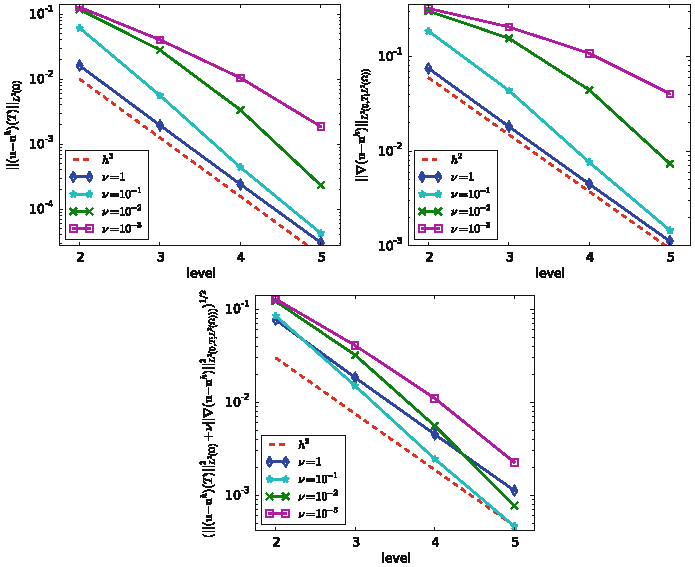
\includegraphics[width=\linewidth]{figures/Chapter_07/Fig_7_01__PDFp396__Bookp386.pdf}
  \captionof{figure}{例题 7.41:误差估计\hyperref[eq:time-dependent-fem-velocity-error]{(7.44)}左端两项误差及其和的收敛曲线.}
  \label{fig:time-dependent-error-convergence}
\end{elegantfigure}
\end{example}

\begin{theorem}[时间连续 Galerkin 有限元法的压力误差估计]
\label{thm:time-dependent-fem-pressure-error}
设定理\hyperref[thm:time-dependent-fem-velocity-error]{7.35} 的假设成立,并进一步假设
\begin{equation}\label{eq:time-dependent-fem-pressure-gradient-regularity}
  \nabla\bm{u}\in L^\infty(0,T;L^2(\Omega))
\end{equation}
且网格剖分族是拟一致的.则对所有 $t\in(0,T]$,有如下误差估计:
\begin{equation}\label{eq:time-dependent-fem-pressure-error}
\begin{aligned}
  \|p-p_h\|_{L^2(0,t;L^2(\Omega))}^2
  &\le C\left(1+\frac{1}{\beta_{\mathrm{is}}^h}\right)^2\\
  &\quad\cdot\inf_{q_h\in L^2(0,t;Q_h)}
       \|p-q_h\|_{L^2(0,t;L^2(\Omega))}^2\\
  &\quad+C\left(\frac{1}{\beta_{\mathrm{is}}^h}\right)^2
       \Bigl[
       \nu^2\|\nabla(\bm{u}-\bm{u}_h)\|_{L^2(0,t;L^2(\Omega))}^2\\
  &\qquad+\|\bm{u}-\bm{u}_h\|_{L^\infty(0,t;L^2(\Omega))}
       \|\nabla(\bm{u}-\bm{u}_h)\|_{L^2(0,t;L^2(\Omega))}\\
  &\qquad\quad\cdot\|\nabla\bm{u}\|_{L^4(0,t;L^2(\Omega))}^2\\
  &\qquad+\|\bm{u}_h\|_{L^\infty(0,t;L^2(\Omega))}
       \|\nabla\bm{u}_h\|_{L^\infty(0,t;L^2(\Omega))}\\
  &\qquad\quad\cdot\|\nabla(\bm{u}-\bm{u}_h)\|_{L^2(0,t;L^2(\Omega))}^2\\
  &\qquad+\|\partial_t(\bm{u}-I_h^{\mathrm{St}}\bm{u})\|_{L^2(0,t;V')}^2
       \Bigr].
\end{aligned}
\end{equation}
\end{theorem}

\begin{proof}
固定 $t\in(0,T]$.与定常问题的证明相同,先分解压力误差,再应用离散 inf-sup 条件\hyperref[eq:discrete-infsup-condition]{(3.51)};参见定理\hyperref[thm:steady-ns-fem-error-pressure]{6.30} 的证明.这样可得到与式\hyperref[eq:steady-ns-pressure-error-infsup]{(6.68)}同型的表达式,其分子为
\begin{equation}\label{eq:time-dependent-pressure-error-numerator}
\begin{aligned}
  &(\partial_t(\bm{u}-\bm{u}_h),\bm{v}_h)
  +\nu(\nabla(\bm{u}-\bm{u}_h),\nabla\bm{v}_h)\\
  &\quad+n_{\mathrm{skew}}(\bm{u},\bm{u},\bm{v}_h)
       -n_{\mathrm{skew}}(\bm{u}_h,\bm{u}_h,\bm{v}_h)
       -(\nabla\cdot\bm{v}_h,p-q_h).
\end{aligned}
\end{equation}

黏性项和含压力的项可像通常那样,利用对偶配对估计或 Cauchy--Schwarz 不等式\hyperref[eq:appendix-a-10]{(A.10)}以及估计\hyperref[eq:divergence-gradient-bound-h01]{(3.41)}得到
\begin{equation}\label{eq:time-dependent-pressure-error-viscous-bound}
  \nu\bigl|(\nabla(\bm{u}-\bm{u}_h),\nabla\bm{v}_h)\bigr|
  \le \nu\|\nabla(\bm{u}-\bm{u}_h)\|_{L^2(\Omega)}
       \|\nabla\bm{v}_h\|_{L^2(\Omega)},
\end{equation}
\begin{equation}\label{eq:time-dependent-pressure-error-pressure-bound}
  |(\nabla\cdot\bm{v}_h,p-q_h)|
  \le \|p-q_h\|_{L^2(\Omega)}
       \|\nabla\bm{v}_h\|_{L^2(\Omega)}.
\end{equation}
这两个估计中的第二个因子会与离散 inf-sup 条件分母中的相应因子约去.

接下来估计对流项.利用分解
\begin{equation}\label{eq:time-dependent-pressure-error-convection-splitting}
\begin{aligned}
  &n_{\mathrm{skew}}(\bm{u},\bm{u},\bm{v}_h)
   -n_{\mathrm{skew}}(\bm{u}_h,\bm{u}_h,\bm{v}_h)\\
  &=n_{\mathrm{skew}}(\bm{u}-\bm{u}_h,\bm{u},\bm{v}_h)
   +n_{\mathrm{skew}}(\bm{u}_h,\bm{u}-\bm{u}_h,\bm{v}_h).
\end{aligned}
\end{equation}
对第一项应用估计\hyperref[eq:steady-ns-conv-estimate-41]{(6.41)},取 $s=1/2$,可得
\begin{equation}\label{eq:time-dependent-pressure-error-convection-bound-1}
\begin{aligned}
  |n_{\mathrm{skew}}(\bm{u}-\bm{u}_h,\bm{u},\bm{v}_h)|
  \le{}&C\|\bm{u}-\bm{u}_h\|_{L^2(\Omega)}^{1/2}
       \|\nabla(\bm{u}-\bm{u}_h)\|_{L^2(\Omega)}^{1/2}\\
  &\quad\cdot\|\nabla\bm{u}\|_{L^2(\Omega)}
       \|\nabla\bm{v}_h\|_{L^2(\Omega)}.
\end{aligned}
\end{equation}
最后一个因子同样与离散 inf-sup 条件分母中的相应因子约去.为估计 $L^2(0,t;L^2(\Omega))$ 范数下的压力误差,还需将其余各项平方并对时间积分.由 Cauchy--Schwarz 不等式,
\[
\begin{aligned}
  &\int_0^t
       \|\bm{u}-\bm{u}_h\|_{L^2(\Omega)}
       \|\nabla(\bm{u}-\bm{u}_h)\|_{L^2(\Omega)}
       \|\nabla\bm{u}\|_{L^2(\Omega)}^2\,\mathrm{d}\tau\\
  &\quad\le
       \|\bm{u}-\bm{u}_h\|_{L^\infty(0,t;L^2(\Omega))}
       \|\nabla(\bm{u}-\bm{u}_h)\|_{L^2(0,t;L^2(\Omega))}
       \|\nabla\bm{u}\|_{L^4(0,t;L^2(\Omega))}^2.
\end{aligned}
\]
其中前两个因子由估计\hyperref[eq:time-dependent-fem-velocity-error]{(7.44)}控制,第三个因子则由假设\hyperref[eq:time-dependent-fem-error-regularity]{(7.43)}控制.

對式\hyperref[eq:time-dependent-pressure-error-convection-splitting]{(7.64)}中的第二項同樣處理,可得
\begin{equation}\label{eq:time-dependent-pressure-error-convection-bound-2}
\begin{aligned}
  |n_{\mathrm{skew}}(\bm{u}_h,\bm{u}-\bm{u}_h,\bm{v}_h)|
  \le{}&C\|\bm{u}_h\|_{L^2(\Omega)}^{1/2}
       \|\nabla\bm{u}_h\|_{L^2(\Omega)}^{1/2}\\
  &\quad\cdot\|\nabla(\bm{u}-\bm{u}_h)\|_{L^2(\Omega)}
       \|\nabla\bm{v}_h\|_{L^2(\Omega)}.
\end{aligned}
\end{equation}
约去 $\|\nabla\bm{v}_h\|_{L^2(\Omega)}$,再平方并在 $(0,t)$ 上积分,得到
\[
\begin{aligned}
  &\int_0^t
       \|\bm{u}_h\|_{L^2(\Omega)}
       \|\nabla\bm{u}_h\|_{L^2(\Omega)}
       \|\nabla(\bm{u}-\bm{u}_h)\|_{L^2(\Omega)}^2\,\mathrm{d}\tau\\
  &\quad\le
       \|\bm{u}_h\|_{L^\infty(0,t;L^2(\Omega))}
       \|\nabla\bm{u}_h\|_{L^\infty(0,t;L^2(\Omega))}
       \|\nabla(\bm{u}-\bm{u}_h)\|_{L^2(0,t;L^2(\Omega))}^2.
\end{aligned}
\]
第一个因子由稳定性估计\hyperref[eq:time-dependent-fem-velocity-stability]{(7.42)}控制.对时刻 $t$ 的 Stokes 投影 $I_h^{\mathrm{St}}\bm{u}$ 应用三角不等式、估计\hyperref[eq:stokes-projection-best-approximation-velocity]{(4.57)}和逆估计\hyperref[eq:appendix-c-35]{(C.35)},并沿用定理\hyperref[thm:time-dependent-fem-velocity-error]{7.35} 证明中的记号,有
\begin{equation}\label{eq:time-dependent-pressure-error-discrete-gradient-bound}
\begin{aligned}
  \|\nabla\bm{u}_h\|_{L^2(\Omega)}
  &\le \|\nabla(\bm{u}-I_h^{\mathrm{St}}\bm{u})\|_{L^2(\Omega)}
       +\|\nabla(I_h^{\mathrm{St}}\bm{u}-\bm{u}_h)\|_{L^2(\Omega)}
       +\|\nabla\bm{u}\|_{L^2(\Omega)}\\
  &\le C\|\nabla\bm{u}\|_{L^2(\Omega)}
       +Ch^{-1}\|I_h^{\mathrm{St}}\bm{u}-\bm{u}_h\|_{L^2(\Omega)}
       +\|\nabla\bm{u}\|_{L^2(\Omega)}\\
  &=C\|\nabla\bm{u}\|_{L^2(\Omega)}\\
  &+Ch^{-1}\|\symbf{\phi}_h\|_{L^2(\Omega)}.
\end{aligned}
\end{equation}
这里 $\symbf{\phi}_h=\bm{u}_h-I_h^{\mathrm{St}}\bm{u}$.由估计\hyperref[eq:time-dependent-fem-error-gronwall]{(7.56)},第二项在 $L^\infty(0,t;L^2(\Omega))$ 中有界;若收敛阶至少为一阶,则 $h^{-1}$ 的负幂可由误差中的 $h$ 阶收敛补偿.对式\hyperref[eq:time-dependent-pressure-error-discrete-gradient-bound]{(7.67)}右端的另一项,则需假设\hyperref[eq:time-dependent-fem-pressure-gradient-regularity]{(7.59)}.在这一假设下,式\hyperref[eq:time-dependent-pressure-error-convection-splitting]{(7.64)}中的第二项也可得到控制.

现在分析式\hyperref[eq:time-dependent-pressure-error-numerator]{(7.61)}中的时间导数项.先将它分解为
\[
\begin{aligned}
  (\partial_t(\bm{u}-\bm{u}_h),\bm{v}_h)
  ={}&(\partial_t(\bm{u}-I_h^{\mathrm{St}}\bm{u}),\bm{v}_h)\\
  &+(\partial_t(I_h^{\mathrm{St}}\bm{u}-\bm{u}_h),\bm{v}_h).
\end{aligned}
\]
第一项利用对偶配对估计可得
\begin{equation}\label{eq:time-dependent-pressure-error-time-derivative-projection}
  |(\partial_t(\bm{u}-I_h^{\mathrm{St}}\bm{u}),\bm{v}_h)|
  \le \|\partial_t(\bm{u}-I_h^{\mathrm{St}}\bm{u})\|_{V'}
       \|\nabla\bm{v}_h\|_{L^2(\Omega)}.
\end{equation}
对另一项作同样处理,并沿用定理\hyperref[thm:time-dependent-fem-velocity-error]{7.35} 证明中的记号,得到
\begin{equation}\label{eq:time-dependent-pressure-error-time-derivative-discrete}
  |(\partial_t(I_h^{\mathrm{St}}\bm{u}-\bm{u}_h),\bm{v}_h)|
  \le \|\partial_t\symbf{\phi}_h\|_{V'}
       \|\nabla\bm{v}_h\|_{L^2(\Omega)}.
\end{equation}

为估计式\hyperref[eq:time-dependent-pressure-error-time-derivative-discrete]{(7.69)}中的第一因子,引入离散 Stokes 算子 $A_h:V_{\mathrm{div}}^h\to V_{\mathrm{div}}^h$,其定义为
\begin{equation}\label{eq:time-dependent-pressure-error-discrete-stokes-operator}
  (A_h\bm{v}_h,\bm{w}_h)
  =(\nabla\bm{v}_h,\nabla\bm{w}_h)
  \qquad\forall\,\bm{v}_h,\bm{w}_h\in V_{\mathrm{div}}^h.
\end{equation}
算子 $A_h$ 对称(自伴)且正定.在式\hyperref[eq:time-dependent-pressure-error-discrete-stokes-operator]{(7.70)}中取 $\bm{w}_h=\bm{v}_h$,可得
\begin{equation}\label{eq:time-dependent-pressure-error-discrete-stokes-norm}
\begin{aligned}
  \|\nabla\bm{v}_h\|_{L^2(\Omega)}
  &=(A_h\bm{v}_h,\bm{v}_h)^{1/2}\\
  &=((A_h)^{1/2}\bm{v}_h,(A_h)^{1/2}\bm{v}_h)^{1/2}
   =\|(A_h)^{1/2}\bm{v}_h\|_{L^2(\Omega)}.
\end{aligned}
\end{equation}
再在式\hyperref[eq:time-dependent-pressure-error-discrete-stokes-operator]{(7.70)}中令两个自变量都等于 $(A_h)^{-1/2}\bm{v}_h$,得到
\begin{equation}\label{eq:time-dependent-pressure-error-discrete-stokes-negative-norm}
  \|\nabla(A_h)^{-1/2}\bm{v}_h\|_{L^2(\Omega)}
  =\|\bm{v}_h\|_{L^2(\Omega)}.
\end{equation}

由 \textcite{AyusoGarciaArchillaNovo2005}(引理 3.11 及式(2.15))可得估计
\[
  \|\partial_t\symbf{\phi}_h\|_{V'}
  \le Ch\|\partial_t\symbf{\phi}_h\|_{L^2(\Omega)}
       +C\|(A_h)^{-1/2}\partial_t\symbf{\phi}_h\|_{L^2(\Omega)}.
\]
右端第一项可由式\hyperref[eq:time-dependent-pressure-error-discrete-stokes-norm]{(7.71)}和逆估计\hyperref[eq:appendix-c-35]{(C.35)}控制:
\[
\begin{aligned}
  Ch\|\partial_t\symbf{\phi}_h\|_{L^2(\Omega)}
  &=Ch\|A_h^{1/2}A_h^{-1/2}
       \partial_t\symbf{\phi}_h\|_{L^2(\Omega)}\\
  &=Ch\|\nabla A_h^{-1/2}
       \partial_t\symbf{\phi}_h\|_{L^2(\Omega)}
   \le C\|A_h^{-1/2}\partial_t\symbf{\phi}_h\|_{L^2(\Omega)}.
\end{aligned}
\]
因此,
\begin{equation}\label{eq:time-dependent-pressure-error-time-derivative-negative-norm}
  \|\partial_t\symbf{\phi}_h\|_{V'}
  \le C\|(A_h)^{-1/2}\partial_t\symbf{\phi}_h\|_{L^2(\Omega)}.
\end{equation}

为控制式\hyperref[eq:time-dependent-pressure-error-time-derivative-negative-norm]{(7.73)}右端,取误差方程\hyperref[eq:time-dependent-fem-error-equation]{(7.48)}中的检验函数
$\bm{v}_h=A_h^{-1}\partial_t\symbf{\phi}_h\in V_{\mathrm{div}}^h$.逐项估计可得
\begin{equation}\label{eq:time-dependent-pressure-error-time-derivative-test}
\begin{aligned}
  (\partial_t\symbf{\phi}_h,
       A_h^{-1}\partial_t\symbf{\phi}_h)
  &=(A_h^{-1/2}\partial_t\symbf{\phi}_h,
       A_h^{-1/2}\partial_t\symbf{\phi}_h)\\
  &=\|A_h^{-1/2}\partial_t\symbf{\phi}_h\|_{L^2(\Omega)}^2.
\end{aligned}
\end{equation}
利用对偶配对估计和式\hyperref[eq:time-dependent-pressure-error-discrete-stokes-negative-norm]{(7.72)},有
\begin{equation}\label{eq:time-dependent-pressure-error-time-derivative-projection-test}
\begin{aligned}
  |(\partial_t\symbf{\eta},A_h^{-1}\partial_t\symbf{\phi}_h)|
  &\le \|\partial_t\symbf{\eta}\|_{V'}
       \|\nabla(A_h^{-1}\partial_t\symbf{\phi}_h)\|_{L^2(\Omega)}\\
  &=\|\partial_t(\bm{u}-I_h^{\mathrm{St}}\bm{u})\|_{V'}
       \|A_h^{-1/2}\partial_t\symbf{\phi}_h\|_{L^2(\Omega)}.
\end{aligned}
\end{equation}
利用离散 Stokes 算子的定义、Cauchy--Schwarz 不等式和式\hyperref[eq:time-dependent-pressure-error-discrete-stokes-norm]{(7.71)},黏性项满足
\begin{equation}\label{eq:time-dependent-pressure-error-viscous-test}
\begin{aligned}
  &\nu\bigl|(\nabla(\bm{u}-\bm{u}_h),
       \nabla(A_h^{-1}\partial_t\symbf{\phi}_h))\bigr|\\
  &\quad\le \nu\|\nabla(\bm{u}-\bm{u}_h)\|_{L^2(\Omega)}
       \|A_h^{-1/2}\partial_t\symbf{\phi}_h\|_{L^2(\Omega)}.
\end{aligned}
\end{equation}
对压力项应用 Cauchy--Schwarz 不等式、式\hyperref[eq:divergence-gradient-bound-h01]{(3.41)}和\hyperref[eq:time-dependent-pressure-error-discrete-stokes-negative-norm]{(7.72)},并按式\hyperref[eq:time-dependent-pressure-error-time-derivative-projection-test]{(7.75)}处理检验函数项,得到
\begin{equation}\label{eq:time-dependent-pressure-error-pressure-test}
\begin{aligned}
  |(\nabla\cdot(A_h^{-1}\partial_t\symbf{\phi}_h),p-q_h)|
  &\le \|p-q_h\|_{L^2(\Omega)}
       \|\nabla(A_h^{-1}\partial_t\symbf{\phi}_h)\|_{L^2(\Omega)}\\
  &=\|p-q_h\|_{L^2(\Omega)}
       \|A_h^{-1/2}\partial_t\symbf{\phi}_h\|_{L^2(\Omega)}.
\end{aligned}
\end{equation}
对非线性项采用推导估计\hyperref[eq:time-dependent-pressure-error-convection-bound-1]{(7.65)}和\hyperref[eq:time-dependent-pressure-error-convection-bound-2]{(7.66)}时的相同方法,并按式\hyperref[eq:time-dependent-pressure-error-time-derivative-projection-test]{(7.75)}处理检验函数,得到
\begin{equation}\label{eq:time-dependent-pressure-error-convection-test}
\begin{aligned}
  &\bigl|n_{\mathrm{skew}}(\bm{u},\bm{u},
       A_h^{-1}\partial_t\symbf{\phi}_h)
       -n_{\mathrm{skew}}(\bm{u}_h,\bm{u}_h,
       A_h^{-1}\partial_t\symbf{\phi}_h)\bigr|\\
  &\quad\le C\Bigl(
       \|\bm{u}-\bm{u}_h\|_{L^2(\Omega)}^{1/2}
       \|\nabla(\bm{u}-\bm{u}_h)\|_{L^2(\Omega)}^{1/2}
       \|\nabla\bm{u}\|_{L^2(\Omega)}\\
  &\qquad\quad+
       \|\bm{u}_h\|_{L^2(\Omega)}^{1/2}
       \|\nabla\bm{u}_h\|_{L^2(\Omega)}^{1/2}
       \|\nabla(\bm{u}-\bm{u}_h)\|_{L^2(\Omega)}
       \Bigr)\\
  &\qquad\cdot\|A_h^{-1/2}\partial_t\symbf{\phi}_h\|_{L^2(\Omega)}.
\end{aligned}
\end{equation}
式\hyperref[eq:time-dependent-pressure-error-time-derivative-projection-test]{(7.75)}至\hyperref[eq:time-dependent-pressure-error-convection-test]{(7.78)}各式右端的第二个因子,可与式\hyperref[eq:time-dependent-pressure-error-time-derivative-test]{(7.74)}中的一个因子约去,从而得到 $\|A_h^{-1/2}\partial_t\symbf{\phi}_h\|_{L^2(\Omega)}$ 的上界.该上界只含有已出现在估计\hyperref[eq:time-dependent-pressure-error-viscous-bound]{(7.62)}、\hyperref[eq:time-dependent-pressure-error-pressure-bound]{(7.63)}、\hyperref[eq:time-dependent-pressure-error-convection-bound-1]{(7.65)}、\hyperref[eq:time-dependent-pressure-error-convection-bound-2]{(7.66)}和\hyperref[eq:time-dependent-pressure-error-time-derivative-projection]{(7.68)}中的项.将其代入式\hyperref[eq:time-dependent-pressure-error-time-derivative-negative-norm]{(7.73)},再代入式\hyperref[eq:time-dependent-pressure-error-time-derivative-discrete]{(7.69)},便完成了对时间导数项的估计.总的来说,该估计所引入的各项与式\hyperref[eq:time-dependent-pressure-error-numerator]{(7.61)}其他项的估计中已有的项相同.

汇总估计\hyperref[eq:time-dependent-pressure-error-viscous-bound]{(7.62)}、\hyperref[eq:time-dependent-pressure-error-pressure-bound]{(7.63)}、\hyperref[eq:time-dependent-pressure-error-convection-bound-1]{(7.65)}、\hyperref[eq:time-dependent-pressure-error-convection-bound-2]{(7.66)}、\hyperref[eq:time-dependent-pressure-error-time-derivative-projection]{(7.68)}和\hyperref[eq:time-dependent-pressure-error-time-derivative-discrete]{(7.69)},对所有 $q_h\in Q_h$ 有
\begin{equation}\label{eq:time-dependent-pressure-error-pointwise}
\begin{aligned}
  \|p_h-q_h\|_{L^2(\Omega)}
  \le \frac{C}{\beta_{\mathrm{is}}^h}\Bigl[{}
       &\nu\|\nabla(\bm{u}-\bm{u}_h)\|_{L^2(\Omega)}\\
       &+\|\bm{u}-\bm{u}_h\|_{L^2(\Omega)}^{1/2}
        \|\nabla(\bm{u}-\bm{u}_h)\|_{L^2(\Omega)}^{1/2}
        \|\nabla\bm{u}\|_{L^2(\Omega)}\\
       &+\|\bm{u}_h\|_{L^2(\Omega)}^{1/2}
        \|\nabla\bm{u}_h\|_{L^2(\Omega)}^{1/2}
        \|\nabla(\bm{u}-\bm{u}_h)\|_{L^2(\Omega)}\\
       &+\|\partial_t(\bm{u}-I_h^{\mathrm{St}}\bm{u})\|_{V'}
        +\|p-q_h\|_{L^2(\Omega)}\Bigr].
\end{aligned}
\end{equation}
最后应用三角不等式
$\|p-p_h\|_{L^2(\Omega)}\le\|p-q_h\|_{L^2(\Omega)}+\|p_h-q_h\|_{L^2(\Omega)}$,代入估计\hyperref[eq:time-dependent-pressure-error-pointwise]{(7.79)},将两边平方并在 $(0,t)$ 上积分,即得压力误差估计\hyperref[eq:time-dependent-fem-pressure-error]{(7.60)}.
\end{proof}

\begin{note}[关于误差估计(7.60)]
\label{note:time-dependent-fem-pressure-error-interpretation}
误差估计\hyperref[eq:time-dependent-fem-pressure-error]{(7.60)}右端含有已由速度误差估计\hyperref[eq:time-dependent-fem-velocity-error]{(7.44)}控制的速度误差,以及该速度误差估计右端出现的项.因此,压力误差 $\|p-p_h\|_{L^2(0,t;L^2(\Omega))}$ 的收敛阶与式\hyperref[eq:time-dependent-fem-velocity-error]{(7.44)}左端速度误差的收敛阶相同.
\end{note}

\begin{example}[解析解对误差估计(7.60)的数值验证]
\label{ex:time-dependent-pressure-error}
采用例题\hyperref[ex:appendix-d-7]{D.7}中的 $Q_2/P_1^{\mathrm{disc}}$ 有限元空间对进行数值模拟.初始网格(层级 0)为图\hyperref[fig:stokes-example-initial-grids]{4.2}所示的不规则四边形网格.时间离散采用 Crank--Nicolson 格式,时间步长均匀取 $\Delta t=10^{-4}$,终止时刻为 $T=5$.

压力误差的计算结果见图\hyperref[fig:time-dependent-pressure-error-convergence]{7.2}.可以清楚地观察到二阶收敛.在本例中,压力误差不依赖于黏度.
\end{example}

\begin{note}[平均量的数值分析]
\label{note:time-dependent-fem-averaged-quantities}
在许多应用中,时间平均量或时空平均量都很重要.然而,到目前为止,关于这些量的数值分析结果仍然很少;例如可参见 \textcite{JohnLaytonManica2007}.
\end{note}

\begin{elegantfigure}[0.64\linewidth]
  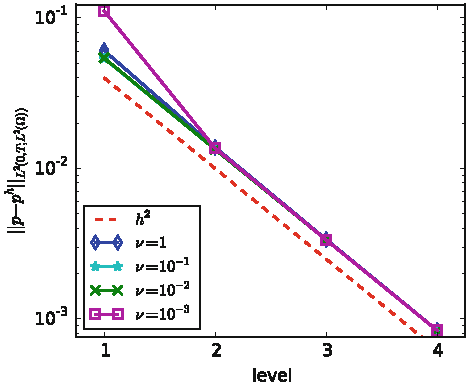
\includegraphics[width=\linewidth]{figures/Chapter_07/Fig_7_02__PDFp403__Bookp393.pdf}
  \captionof{figure}{例题 7.44:压力误差的收敛曲线.}
  \label{fig:time-dependent-pressure-error-convergence}
\end{elegantfigure}

\section{导致耦合问题的时间离散}
\label{sec:time-discretizations-coupled-problems}

\subsection{\texorpdfstring{$\theta$}{θ}-格式作为时间离散方法}
\label{subsec:theta-schemes}

\begin{note}[$\theta$-格式的基本应用思路]
\label{note:theta-scheme-principal-approach}
为完全离散并线性化方程组\hyperref[eq:time-dependent-ns-strong]{(7.1)},$\theta$-格式采用以下步骤:
\begin{enumerate}
  \item 对方程组\hyperref[eq:time-dependent-ns-strong]{(7.1)}作时间半离散.时间半离散后,在每个离散时刻都得到一个非线性鞍点型方程组.
  \item 写出变分形式并作线性化.将非线性方程组改写为变分问题,再将非线性变分问题线性化.
  \item 对线性系统作空间离散.求解非线性问题的迭代过程中,每一步都会产生一个线性系统;随后用有限元方法对该系统作空间离散,例如选用满足 inf-sup 条件的有限元空间对.
\end{enumerate}
这种方法先离散时间、再离散空间,也称为 Rothe 方法或水平线法.各步骤将在本节中详细说明.另一种方法先作空间离散以得到常微分方程组,再对时间离散,称为垂直线法.
\index{theta-format@$\theta$-格式}\index{Rothe method@Rothe 方法}\index{horizontal-lines-method@水平线法}\index{vertical-lines-method@垂直线法}
\end{note}

\begin{note}[记号约定]
\label{note:time-discretization-notation}
设 $t_n\in[0,T]$.在离散时刻 $t_n$ 取值的量用下标 $n$ 表示.从离散时刻 $t_n$ 到下一个离散时刻 $t_{n+1}$ 的时间步长记为 $\Delta t_{n+1}$,即
\[
  \Delta t_{n+1}=t_{n+1}-t_n.
\]
\end{note}

\begin{note}[Navier--Stokes 方程的单步 $\theta$-格式]
\label{note:one-step-theta-scheme}
取 $\theta\in[0,1]$,考察从 $t_n$ 到 $t_{n+1}$ 的时间步.Navier--Stokes 方程的单步 $\theta$-格式可写为
\begin{equation}\label{eq:theta-scheme-one-step}
\begin{aligned}
  \frac{\bm{u}_{n+1}}{\Delta t_{n+1}}
  &+\theta\Bigl[-\nu\Delta\bm{u}_{n+1}
       +(\bm{u}_{n+1}\cdot\nabla)\bm{u}_{n+1}\Bigr]\\
  &+\nabla p_{n+1}
       =\frac{\bm{u}_n}{\Delta t_{n+1}}\\
  &\quad-(1-\theta)\Bigl[-\nu\Delta\bm{u}_n\\
  &\qquad+(\bm{u}_n\cdot\nabla)\bm{u}_n\Bigr]\\
  &\quad+(1-\theta)\bm{f}_n+\theta\bm{f}_{n+1},\\
  0&=\nabla\cdot\bm{u}_{n+1}.
\end{aligned}
\end{equation}
\end{note}

\begin{example}[显式与隐式 Euler 格式、Crank--Nicolson 格式]
\label{ex:time-dependent-crank-nicolson}
三个常用的单步 $\theta$-格式——前向与后向 Euler 格式以及 Crank--Nicolson 格式——由 $\theta$ 的相应取值给出:
\begin{itemize}
  \item $\theta=0$:前向(显式)Euler 格式;
  \item $\theta=0.5$:Crank--Nicolson 格式;
  \item $\theta=1$:后向(隐式)Euler 格式.
\end{itemize}
\index{explicit-Euler@前向 Euler 格式}\index{implicit-Euler@后向 Euler 格式}\index{Crank-Nicolson@Crank--Nicolson 格式}
关于这些格式,还有几点值得说明.更详细的讨论将在数值算例之后的笔记\hyperref[note:theta-scheme-comments]{7.59} 中给出.
\begin{itemize}
  \item \textit{前向或显式 Euler 格式.}黏性项与扩散项形式相同,会使时间方向上的常微分方程组成为刚性问题;参见 \textcite{HairerWanner2010}(第 6 页).常微分方程数值分析表明,对刚性问题,为获得稳定模拟,显式格式必须采用很小的时间步长.对于 Navier--Stokes 方程,时间步长通常小到使模拟效率很低.因此,不建议用前向 Euler 格式或其他显式格式离散不可压缩 Navier--Stokes 方程.
  \item \textit{后向或隐式 Euler 格式.}这是一阶格式,应用相当广泛.不过,文献中已有研究指出,参见 \textcite{JohnMatthiesRang2006a};例题\hyperref[ex:time-dependent-accuracy-comparison]{7.58} 也将说明,将后向 Euler 格式与高阶空间离散结合时,所得结果可能比采用高阶时间离散时的结果精度差得多.
  \item \textit{Crank--Nicolson 格式(梯形公式).}Crank--Nicolson 格式是二阶格式,应用非常普遍.
  \item \textit{一般情形.}对于时间变化的自适应网格,\textcite{BesierWollner2012} 观察并分析了单步格式中压力近似的缺陷.该文研究了若干处理方案,最终认为,最佳做法是在网格改变后的至少一个时间步中采用例题\hyperref[ex:fractional-step-theta-scheme]{7.52} 所述的分步 $\theta$-格式.
\end{itemize}
\end{example}

\begin{note}[关于不可压缩约束]
\label{note:theta-scheme-incompressibility}
\begin{itemize}
  \item 式\hyperref[eq:theta-scheme-one-step]{(7.80)}中的时间导数是在 $t_n+\theta\Delta t_{n+1}$ 处近似的;参见式\hyperref[eq:midpoint-difference-consistency]{(7.94)}.因此,速度也近似于这一时刻的值,而压力则是该速度对应的拉格朗日乘子.例如,在 Crank--Nicolson 格式下,计算所得解近似于 $(\bm{u}_{n+1/2},p_{n+1/2})$.若希望在时刻 $t_{n+1}$ 得到较准确的压力近似,则可将 Crank--Nicolson 格式中的压力项改为
  \[
    \frac12(p_{n+1}+p_n),
  \]
  例如参见 \textcite{Rang2008}.不过,该格式在第一步中需要初始时刻的压力;关于这一问题,见笔记\hyperref[note:time-dependent-initial-pressure]{7.29}.

  \item 与 Stokes 方程的式\hyperref[eq:stokes-abstract-weak]{(4.3)}类似,时间步\hyperref[eq:theta-scheme-one-step]{(7.80)}的变分形式可在乘积空间中写出:求 $(\bm{u}_{n+1},p_{n+1})\in V\times Q$,使得对所有 $(\bm{v},q)\in V\times Q$,
  \[
  \begin{aligned}
    \frac{1}{\Delta t_{n+1}}(\bm{u}_{n+1},\bm{v})
    &+\theta\Bigl[\nu(\nabla\bm{u}_{n+1},\nabla\bm{v})
       +((\bm{u}_{n+1}\cdot\nabla)\bm{u}_{n+1},\bm{v})\Bigr]\\
    &+(\nabla\cdot\bm{u}_{n+1},q)
       -(\nabla\cdot\bm{v},p_{n+1})\\
    &=\frac{1}{\Delta t_{n+1}}(\bm{u}_n,\bm{v})\\
    &\quad-(1-\theta)\Bigl[\nu(\nabla\bm{u}_n,\nabla\bm{v})
       +((\bm{u}_n\cdot\nabla)\bm{u}_n,\bm{v})\Bigr]\\
    &\quad+(1-\theta)\langle\bm{f}_n,\bm{v}\rangle_{V',V}
       +\theta\langle\bm{f}_{n+1},\bm{v}\rangle_{V',V}.
  \end{aligned}
  \]
  等价地,将整个问题乘以 $\Delta t_{n+1}$ 后,可得
  \begin{equation}\label{eq:theta-scheme-variational}
  \begin{aligned}
    &(\bm{u}_{n+1},\bm{v})
      +\theta\Delta t_{n+1}\Bigl[\nu(\nabla\bm{u}_{n+1},\nabla\bm{v})
       +((\bm{u}_{n+1}\cdot\nabla)\bm{u}_{n+1},\bm{v})\Bigr]\\
    &\quad+\Delta t_{n+1}(\nabla\cdot\bm{u}_{n+1},q)
       -\Delta t_{n+1}(\nabla\cdot\bm{v},p_{n+1})\\
    &=(\bm{u}_n,\bm{v})
       -(1-\theta)\Delta t_{n+1}\Bigl[\nu(\nabla\bm{u}_n,\nabla\bm{v})
       +((\bm{u}_n\cdot\nabla)\bm{u}_n,\bm{v})\Bigr]\\
    &\quad+(1-\theta)\Delta t_{n+1}\langle\bm{f}_n,\bm{v}\rangle_{V',V}
       +\theta\Delta t_{n+1}\langle\bm{f}_{n+1},\bm{v}\rangle_{V',V}.
  \end{aligned}
  \end{equation}
  在式\hyperref[eq:theta-scheme-variational]{(7.81)}中取 $(\bm{v},q)=(\bm{u},p)$,可见散度项相消.这与定常问题的分析相同,例如引理\hyperref[lem:steady-ns-stability]{6.21} 的证明.因此,就这一点而言,式\hyperref[eq:theta-scheme-variational]{(7.81)}具有与定常问题变分形式相同的性质.

  相应的式\hyperref[eq:theta-scheme-variational]{(7.81)}强形式为
  \begin{equation}\label{eq:theta-scheme-strong}
  \begin{aligned}
    \bm{u}_{n+1}
    &+\theta\Delta t_{n+1}\Bigl[-\nu\Delta\bm{u}_{n+1}\\
    &\quad+(\bm{u}_{n+1}\cdot\nabla)\bm{u}_{n+1}\Bigr]\\
    &+\Delta t_{n+1}\nabla p_{n+1}=\bm{u}_n\\
    &\quad-(1-\theta)\Delta t_{n+1}\Bigl[-\nu\Delta\bm{u}_n\\
    &\qquad+(\bm{u}_n\cdot\nabla)\bm{u}_n\Bigr]\\
    &\quad+(1-\theta)\Delta t_{n+1}\bm{f}_n
       +\theta\Delta t_{n+1}\bm{f}_{n+1},\\
    0&=\Delta t_{n+1}\nabla\cdot\bm{u}_{n+1}.
  \end{aligned}
  \end{equation}
  可见,散度约束乘上了 $\Delta t_{n+1}$.当然,也可以只将式\hyperref[eq:theta-scheme-one-step]{(7.80)}中的动量方程乘以 $\Delta t_{n+1}$,而保持连续性方程不变;这样得到的问题在数学上与式\hyperref[eq:theta-scheme-variational]{(7.81)}等价.除这一注记中给出的缩放理由外,根据我们的经验,对含缩放散度约束的问题\hyperref[eq:theta-scheme-variational]{(7.81)}作数值求解效率更高.本专著所列所有含时问题的模拟,均按式\hyperref[eq:theta-scheme-variational]{(7.81)}或\hyperref[eq:theta-scheme-strong]{(7.82)}对散度约束作了时间步长缩放.
\end{itemize}
\end{note}

\begin{note}[Navier--Stokes 方程的一般 $\theta$-格式]
\label{note:general-theta-scheme}
Navier--Stokes 方程组\hyperref[eq:time-dependent-ns-strong]{(7.1)}的一般 $\theta$-格式在某个时间步中的形式为
\begin{equation}\label{eq:general-theta-scheme}
\begin{aligned}
  \frac{\bm{u}_{k+1}}{\Delta t_{n+1}}
  &+\theta_1\Bigl[-\nu\Delta\bm{u}_{k+1}
       +(\bm{u}_{k+1}\cdot\nabla)\bm{u}_{k+1}\Bigr]\\
  &+\frac{\Delta t_{k+1}}{\Delta t_{n+1}}\nabla p_{k+1}
       =\frac{\bm{u}_k}{\Delta t_{n+1}}\\
  &\quad-\theta_2\Bigl[-\nu\Delta\bm{u}_k\\
  &\qquad+(\bm{u}_k\cdot\nabla)\bm{u}_k\Bigr]
       +\theta_3\bm{f}_k+\theta_4\bm{f}_{k+1},\\
  0&=\Delta t_{k+1}\nabla\cdot\bm{u}_{k+1},
\end{aligned}
\end{equation}
其中参数为 $\theta_1,\ldots,\theta_4$.注意,时间指标 $k$ 与 $n$ 不同.
\end{note}

\begin{example}[分步 $\theta$-格式]
\label{ex:fractional-step-theta-scheme}
\textcite{BristeauGlowinskiPeriaux1987} 提出的分步 $\theta$-格式由三个式\hyperref[eq:general-theta-scheme]{(7.83)}形式的步骤组成.该格式有 FS0 和 FS1 两个变体,列于表\hyperref[tab:fractional-step-theta-variants]{7.1}.其中
\[
  \theta=1-\frac{\sqrt{2}}{2},\qquad
  \widetilde{\theta}=1-2\theta,\qquad
  \tau=\frac{\widetilde{\theta}}{1-\theta},\qquad
  \eta=1-\tau.
\]
\index{fractional-step-theta@分步 $\theta$-格式}
分步 $\theta$-格式巧妙地组合了三个一阶单步格式,从而得到强 A-稳定的二阶格式.FS1 只需在 $t_n$ 和 $t_{n+1}-\theta\Delta t_{n+1}$ 处计算 $\bm{f}$;FS0 还需额外在 $t_n+\theta\Delta t_{n+1}$ 和 $t_{n+1}$ 处计算.两种变体都是二阶格式,但 FS1 对关于时间 $t$ 的二次多项式不能精确积分.在稳定性等其他基本性质方面,两者大致相同.关于二维 Navier--Stokes 方程的数值结果,\textcite{JohnMatthiesRang2006a} 表明 FS0 通常比 FS1 精确得多.因此,若计算右端项的代价不高,应优先采用 FS0.

\begin{eleganttable}
\centering
\captionof{table}{分步 $\theta$-格式的两个变体}
\label{tab:fractional-step-theta-variants}
\scriptsize
\setlength{\tabcolsep}{2.5pt}
\renewcommand{\arraystretch}{1.16}
\resizebox{\linewidth}{!}{%
\begin{tabular}{c|cccc|cc|c|c}
\hline
 & $\theta_1$ & $\theta_2$ & $\theta_3$ & $\theta_4$
 & $t_k$ & $t_{k+1}$ & $\Delta t_{k+1}$ & 阶数 \\
\hline
FS0 & $\tau\theta$ & $\eta\theta$ & $\eta\theta$ & $\tau\theta$
    & $t_n$ & $t_n+\theta\Delta t_{n+1}$ & $\theta\Delta t_{n+1}$ & 2 \\
    & $\eta\widetilde{\theta}$ & $\tau\widetilde{\theta}$
    & $\tau\widetilde{\theta}$ & $\eta\widetilde{\theta}$
    & $t_n+\theta\Delta t_{n+1}$ & $t_{n+1}-\theta\Delta t_{n+1}$
    & $\widetilde{\theta}\Delta t_{n+1}$ & \\
    & $\tau\theta$ & $\eta\theta$ & $\eta\theta$ & $\tau\theta$
    & $t_{n+1}-\theta\Delta t_{n+1}$ & $t_{n+1}$
    & $\theta\Delta t_{n+1}$ & \\
\hline
FS1 & $\tau\theta$ & $\eta\theta$ & $\theta$ & $0$
    & $t_n$ & $t_n+\theta\Delta t_{n+1}$ & $\theta\Delta t_{n+1}$ & 2 \\
    & $\eta\widetilde{\theta}$ & $\tau\widetilde{\theta}$
    & $0$ & $\widetilde{\theta}$
    & $t_n+\theta\Delta t_{n+1}$ & $t_{n+1}-\theta\Delta t_{n+1}$
    & $\widetilde{\theta}\Delta t_{n+1}$ & \\
    & $\tau\theta$ & $\eta\theta$ & $\theta$ & $0$
    & $t_{n+1}-\theta\Delta t_{n+1}$ & $t_{n+1}$
    & $\theta\Delta t_{n+1}$ & \\
\hline
\end{tabular}%
}
\end{eleganttable}
\end{example}

\begin{note}[$\theta$-格式的统一表示]
\label{note:theta-scheme-comments}
注意,单步 $\theta$-格式\hyperref[eq:theta-scheme-one-step]{(7.80)}在参数取适当值时,可写成一般 $\theta$-格式\hyperref[eq:general-theta-scheme]{(7.83)};见表\hyperref[tab:one-step-theta-parameters]{7.2}.因此,式\hyperref[eq:general-theta-scheme]{(7.83)}使所有已介绍格式都能用同一个公式实现,并可通过设置四个参数来选择具体格式.本节之后关于 $\theta$-格式的讨论,都将采用一般 $\theta$-格式\hyperref[eq:general-theta-scheme]{(7.83)}.

\begin{eleganttable}
\centering
\captionof{table}{写成一般 $\theta$-格式(7.83)时单步 $\theta$-格式的参数}
\label{tab:one-step-theta-parameters}
\scriptsize
\setlength{\tabcolsep}{3pt}
\renewcommand{\arraystretch}{1.18}
\resizebox{\linewidth}{!}{%
\begin{tabular}{l|cccc|ccc|c}
\hline
格式 & $\theta_1$ & $\theta_2$ & $\theta_3$ & $\theta_4$
 & $t_k$ & $t_{k+1}$ & $\Delta t_{k+1}$ & 阶数 \\
\hline
前向 Euler 格式 & $0$ & $1$ & $1$ & $0$
 & $t_n$ & $t_{n+1}$ & $\Delta t_{n+1}$ & 1 \\
后向 Euler 格式(BWE) & $1$ & $0$ & $0$ & $1$
 & $t_n$ & $t_{n+1}$ & $\Delta t_{n+1}$ & 1 \\
Crank--Nicolson 格式(CN) & $0.5$ & $0.5$ & $0.5$ & $0.5$
 & $t_n$ & $t_{n+1}$ & $\Delta t_{n+1}$ & 2 \\
\hline
\end{tabular}%
}
\end{eleganttable}
\end{note}

\begin{note}[变分形式]
\label{note:general-theta-variational}
将式\hyperref[eq:general-theta-scheme]{(7.83)}的解用有限元方法近似时,需要先写出其变分形式.通常的推导方式是将式\hyperref[eq:general-theta-scheme]{(7.83)}中的方程乘以检验函数,在区域 $\Omega$ 上积分并分部积分;再将整个问题按 $\Delta t_{n+1}$ 缩放.由此得到:求 $(\bm{u}_{k+1},p_{k+1})\in V\times Q$,使得对所有 $(\bm{v},q)\in V\times Q$,
\begin{equation}\label{eq:general-theta-variational}
\begin{aligned}
  &(\bm{u}_{k+1},\bm{v})
     +\theta_1\Delta t_{n+1}\Bigl[
       \nu(\nabla\bm{u}_{k+1},\nabla\bm{v})\\
  &\qquad+((\bm{u}_{k+1}\cdot\nabla)\bm{u}_{k+1},\bm{v})\Bigr]
       -\Delta t_{k+1}(\nabla\cdot\bm{v},p_{k+1})\\
  &=(\bm{u}_k,\bm{v})
       -\theta_2\Delta t_{n+1}\Bigl[
       \nu(\nabla\bm{u}_k,\nabla\bm{v})\\
  &\qquad+((\bm{u}_k\cdot\nabla)\bm{u}_k,\bm{v})\Bigr]
       +\theta_3\Delta t_{n+1}\langle\bm{f}_k,\bm{v}\rangle_{V',V}\\
  &\qquad+\theta_4\Delta t_{n+1}
       \langle\bm{f}_{k+1},\bm{v}\rangle_{V',V},\\
  0&=\Delta t_{k+1}(\nabla\cdot\bm{u}_{k+1},q).
\end{aligned}
\end{equation}
当然,也可以采用第\hyperref[subsec:steady-ns-nonlinear-term]{6.1.2 节}讨论的其他对流项形式.为简洁起见,以下仅以对流形式说明.
\end{note}

\begin{note}[变分形式的线性化]
\label{note:general-theta-linearization}
非线性系统\hyperref[eq:general-theta-variational]{(7.84)}从初始猜测 $(\bm{u}_{k+1}^{(0)},p_{k+1}^{(0)})$ 出发,通过迭代求解.必须对非线性对流项作线性化;可采用与定常 Navier--Stokes 方程相同的线性化方法,见第\hyperref[sec:steady-ns-iterations]{6.3 节}.

已知速度场 $\bm{u}_{k+1}^{(m)}$ 时,不动点迭代(也称 Picard 迭代)作如下近似:
\index{不动点迭代}
\index{Picard 迭代}
\[
  (\bm{u}_{k+1}^{(m+1)}\cdot\nabla)\bm{u}_{k+1}^{(m+1)}
  \approx
  (\bm{u}_{k+1}^{(m)}\cdot\nabla)\bm{u}_{k+1}^{(m+1)}.
\]
因此,求解式\hyperref[eq:general-theta-variational]{(7.84)}的 Picard 不动点迭代如下:给定 $(\bm{u}_{k+1}^{(m)},p_{k+1}^{(m)})$,通过求解下列问题得到迭代值 $(\bm{u}_{k+1}^{(m+1)},p_{k+1}^{(m+1)})$:
\begin{equation}\label{eq:general-theta-picard}
\begin{aligned}
  &(\bm{u}_{k+1}^{(m+1)},\bm{v})
   +\theta_1\Delta t_{n+1}\Bigl[
     \nu(\nabla\bm{u}_{k+1}^{(m+1)},\nabla\bm{v})\\
  &\qquad+((\bm{u}_{k+1}^{(m)}\cdot\nabla)
      \bm{u}_{k+1}^{(m+1)},\bm{v})\Bigr]
   -\Delta t_{k+1}(\nabla\cdot\bm{v},p_{k+1}^{(m+1)})\\
  &=(\bm{u}_k,\bm{v})
    +\theta_3\Delta t_{n+1}\langle\bm{f}_k,\bm{v}\rangle_{V',V}
    +\theta_4\Delta t_{n+1}\langle\bm{f}_{k+1},\bm{v}\rangle_{V',V}\\
  &\quad-\theta_2\Delta t_{n+1}\Bigl[
      \nu(\nabla\bm{u}_k,\nabla\bm{v})
      +((\bm{u}_k\cdot\nabla)\bm{u}_k,\bm{v})\Bigr],\\
  0&=\Delta t_{k+1}(\nabla\cdot\bm{u}_{k+1}^{(m+1)},q),
  \qquad \forall (\bm{v},q)\in V\times Q.
\end{aligned}
\end{equation}
其中 $m=0,1,2,\ldots$.式\hyperref[eq:general-theta-picard]{(7.85)}属于 Oseen 型问题,参见式\hyperref[eq:oseen-weak]{(5.2)};该迭代过程中,方程右端保持不变.

对于 Newton 方法,非线性对流项作如下线性化:
\index{Newton 方法}
\[
\begin{aligned}
  (\bm{u}_{k+1}^{(m+1)}\cdot\nabla)
       \bm{u}_{k+1}^{(m+1)}
  &\approx (\bm{u}_{k+1}^{(m)}\cdot\nabla)
       \bm{u}_{k+1}^{(m+1)}\\
  &\quad+(\bm{u}_{k+1}^{(m+1)}\cdot\nabla)
       \bm{u}_{k+1}^{(m)}
       -(\bm{u}_{k+1}^{(m)}\cdot\nabla)
       \bm{u}_{k+1}^{(m)}.
\end{aligned}
\]
于是迭代问题如下:给定 $(\bm{u}_{k+1}^{(m)},p_{k+1}^{(m)})$,通过求解下列问题得到迭代值 $(\bm{u}_{k+1}^{(m+1)},p_{k+1}^{(m+1)})$:
\begin{equation}\label{eq:general-theta-newton}
\begin{aligned}
  &(\bm{u}_{k+1}^{(m+1)},\bm{v})
   +\theta_1\Delta t_{n+1}\Bigl[
     \nu(\nabla\bm{u}_{k+1}^{(m+1)},\nabla\bm{v})\\
  &\qquad+((\bm{u}_{k+1}^{(m)}\cdot\nabla)
       \bm{u}_{k+1}^{(m+1)},\bm{v})
       +((\bm{u}_{k+1}^{(m+1)}\cdot\nabla)
       \bm{u}_{k+1}^{(m)},\bm{v})\Bigr]\\
  &\quad-\Delta t_{k+1}(\nabla\cdot\bm{v},p_{k+1}^{(m+1)})\\
  &=(\bm{u}_k,\bm{v})
    +\theta_3\Delta t_{n+1}\langle\bm{f}_k,\bm{v}\rangle_{V',V}
    +\theta_4\Delta t_{n+1}\langle\bm{f}_{k+1},\bm{v}\rangle_{V',V}\\
  &\quad+\theta_1\Delta t_{n+1}
       ((\bm{u}_{k+1}^{(m)}\cdot\nabla)
       \bm{u}_{k+1}^{(m)},\bm{v})\\
  &\quad-\theta_2\Delta t_{n+1}\Bigl[
       \nu(\nabla\bm{u}_k,\nabla\bm{v})
       +((\bm{u}_k\cdot\nabla)\bm{u}_k,\bm{v})\Bigr],\\
  0&=\Delta t_{k+1}(\nabla\cdot\bm{u}_{k+1}^{(m+1)},q),
  \qquad \forall (\bm{v},q)\in V\times Q.
\end{aligned}
\end{equation}
其中 $m=0,1,2,\ldots$.初始猜测可取上一时间步的解,即 $(\bm{u}_{k+1}^{(0)},p_{k+1}^{(0)})=(\bm{u}_k,p_k)$,也可由一个以上的历史时间步外推得到.按本节所述方法对 Navier--Stokes 方程\hyperref[eq:time-dependent-ns-strong]{(7.1)}作数值近似时,每个离散时刻都需要反复求解式\hyperref[eq:general-theta-picard]{(7.85)}或\hyperref[eq:general-theta-newton]{(7.86)}这类线性鞍点问题.
\end{note}

\begin{note}[Picard 迭代与 Newton 方法的比较]
\label{note:time-dependent-picard-newton-comparison}
关于 Picard 迭代与 Newton 方法的比较,第 6 章定常 Navier--Stokes 方程中给出的相同结论仍然适用,例如笔记\hyperref[note:steady-ns-newton-convergence]{6.44}和笔记\hyperref[note:steady-ns-velocity-coupling-cost]{6.46}.

与定常问题的一个主要区别是,在含时问题中,可以利用前一离散时刻的解,甚至利用多个先前解作外推,从而得到较好的初始迭代值.因此,求解一个时间步所需的迭代次数通常远少于定常问题;经验表明,时间步越短,所需迭代次数越少.

对于采用迭代求解器并对线性系统作非精确求解的情形,\textcite{JohnMatthiesRang2006a} 关于三维绕圆柱流动的数值研究表明,在该例中 Picard 迭代的效率显著高于 Newton 方法.第\hyperref[note:chapter9-solver-choice]{9.5 条笔记}还将讨论三维问题通常应采用迭代求解器;另见例题\hyperref[ex:time-dependent-picard-vs-newton]{7.57}.
\end{note}

\begin{example}[\enspace (Picard 迭代与 Newton 方法的比较)]
\label{ex:time-dependent-picard-vs-newton}
本例考虑一个具有解析解的三维问题,见例题\hyperref[ex:appendix-d-10]{D.10}.计算取黏度 $\nu=10^{-3}$.区域剖分采用由立方体组成的六面体网格(第 0 层含 8 个立方体);有限元空间选用 $Q_2/Q_1$ 元对;时间离散采用等步长 $\Delta t=0.01$ 的 Crank--Nicolson 格式,时间区间为 $[0,0.1]$;初始迭代值取前一离散时刻的解.

表\hyperref[tab:time-dependent-picard-newton]{7.3} 给出了上述设置的结果.总体观察与定常问题相同,参见例题\hyperref[ex:steady-ns-picard-vs-newton]{6.47}.通常,Newton 方法所需的迭代次数少于 Picard 方法;使用直接求解器求解线性系统时,Newton 方法的迭代次数会更少.

表\hyperref[tab:time-dependent-picard-newton]{7.3} 还列出了求解一个线性系统所需的时间.以第 2 层上 Picard 方法采用非精确求解时的平均耗时为基准(100\% $\approx 3$ 秒).非精确求解器采用带耦合多重网格预条件子的 FGMRES 方法,见笔记\hyperref[note:chapter9-multigrid-preconditioner]{9.6}和第\hyperref[subsec:chapter9-iterative-solvers]{9.2.2 节}.稀疏直接求解器采用 UMFPACK,见笔记\hyperref[note:chapter9-solver-choice]{9.5}.可以看到,在第 2 层上,两种求解器的计算时间处于同一量级.因此,Newton 方法配合直接求解器是效率最高的方案.网格再细化一次,未知量数量便增至原来的 8 倍.结果表明,非精确求解器的扩展性几乎达到最优,而直接求解器的效率则显著下降.因此,在第 3 层上,Newton 方法配合非精确求解器最快.

\begin{eleganttable}
\centering
\captionof{table}{例题\hyperref[ex:time-dependent-picard-vs-newton]{7.57}}
\label{tab:time-dependent-picard-newton}
\scriptsize
\setlength{\tabcolsep}{2.8pt}
\renewcommand{\arraystretch}{1.12}
\resizebox{\linewidth}{!}{%
\begin{tabular}{l|cc|cc}
\hline
 & \multicolumn{2}{c|}{第 2 层} & \multicolumn{2}{c}{第 3 层}\\
\hline
速度/压力自由度 & \multicolumn{2}{c|}{14,739/729}
                & \multicolumn{2}{c}{107,811/4913}\\
 & 线性系统数 & 单个系统相对耗时
 & 线性系统数 & 单个系统相对耗时\\
\hline
Picard／非精确 & 33 & 100 & 23 & 824\\
Picard／直接 & 33 & 140 & 22 & 8989\\
Newton／非精确 & 23 & 101 & 12 & 804\\
Newton／直接 & 11 & 142 & 11 & 8932\\
\hline
\end{tabular}%
}
\par\smallskip
\footnotesize 求解数值解(共十个时间步)时线性系统的求解次数,以及求解单个线性系统所需的相对计算时间(Picard 方法采用非精确求解时取 100\%,约为 3 秒).
\end{eleganttable}
\end{example}

\begin{example}[\enspace (例题 D.9 的精度研究)]
\label{ex:time-dependent-accuracy}\label{ex:time-dependent-accuracy-comparison}
本例考察例题\hyperref[ex:appendix-d-9]{D.9}中定义的二维绕圆柱流动,出口采用 do-nothing 边界条件\hyperref[eq:appendix-d-30]{(D.30)}.

结果针对三种隐式 $\theta$-格式给出:后向 Euler 格式、Crank--Nicolson 格式和分步 $\theta$-格式.\index{后向 Euler 格式}\index{分步 $\theta$-格式}此问题对所有时刻均有 $\bm{f}=\bm{0}$,因此 FS0 与 FS1 完全相同.空间离散采用 $Q_2/P_1^{\mathrm{disc}}$ 元对;初始网格(第 0 层)为图\hyperref[fig:steady-ns-cylinder-initial-grids]{6.5}所示的四边形网格.表\hyperref[tab:time-dependent-cylinder-dofs]{7.4}列出了不同细化层级的自由度数.

\begin{eleganttable}[0.62\linewidth]
\centering
\captionof{table}{例题\hyperref[ex:time-dependent-accuracy]{7.58}}
\label{tab:time-dependent-cylinder-dofs}
\scriptsize
\setlength{\tabcolsep}{4pt}
\renewcommand{\arraystretch}{1.12}
\resizebox{\linewidth}{!}{%
\begin{tabular}{c|ccc}
\hline
层级 & 速度 & 压力 & 总计\\
\hline
3 & 27,232 & 9,984 & 37,216\\
4 & 107,712 & 39,936 & 147,648\\
5 & 428,416 & 159,744 & 588,160\\
\hline
\end{tabular}%
}
\par\smallskip
\footnotesize 空间自由度数(包括 Dirichlet 节点).
\end{eleganttable}

每个离散时刻的非线性系统都求解至残量向量的欧几里得范数小于 $10^{-10}$.阻力系数和升力系数按式\hyperref[eq:appendix-d-16]{(D.16)}和式\hyperref[eq:appendix-d-17]{(D.17)}计算,具体方法与例题\hyperref[ex:steady-ns-flow-around-cylinder]{6.36}相同.式(D.16)和式(D.17)中的时间导数采用后向差分公式近似:
\[
  \partial_t\bm{u}_{n+1}^{h}
  \approx\frac{\bm{u}_{n+1}^{h}-\bm{u}_{n}^{h}}{\Delta t_{n+1}}.
\]

\begin{elegantfigure}[\linewidth]
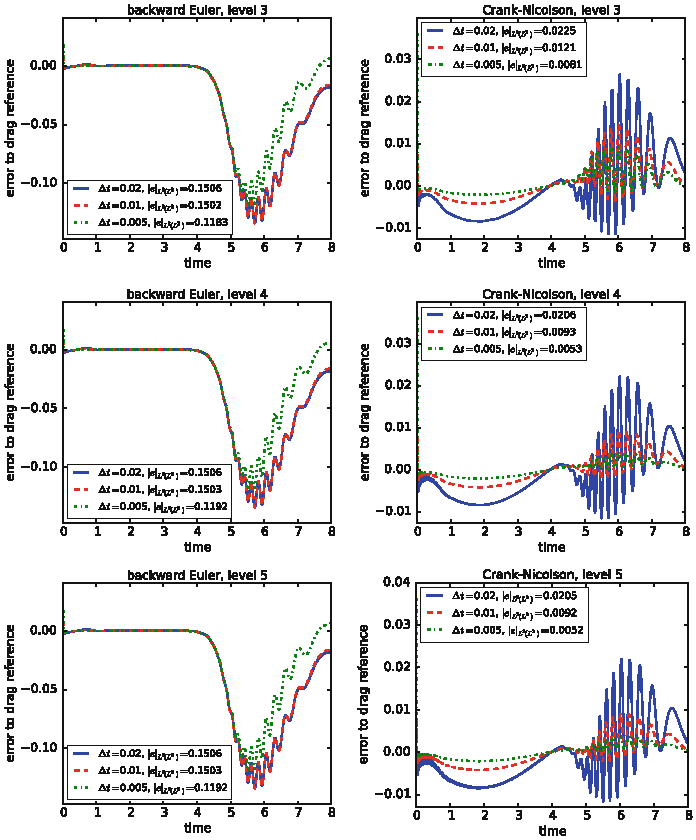
\includegraphics[width=\linewidth]{figures/Chapter_07/Fig_7_03__PDFp411__Bookp401.pdf}
\captionof{figure}{例题\hyperref[ex:time-dependent-accuracy]{7.58}:阻力系数相对于图\hyperref[fig:appendix-d-10]{D.10}中参考曲线的误差;$Q_2/P_1^{\mathrm{disc}}$ 元对,第 3--5 层(自上而下);左:后向 Euler 格式,右:Crank--Nicolson 格式.两侧均比较了不同的时间步长.}
\label{fig:time-dependent-drag-error}
\end{elegantfigure}

图\hyperref[fig:time-dependent-drag-error]{7.3}--\hyperref[fig:time-dependent-pressure-error]{7.8}给出了计算结果.可以看到,在所有时间离散格式中,后向 Euler 格式所得结果的精度明显最低.本例中,时间误差和空间误差都很重要;采用后向 Euler 格式时,时间误差占主导.若要达到二阶时间格式所能达到的相近误差水平,必须显著缩小时间步长.

\begin{elegantfigure}[\linewidth]
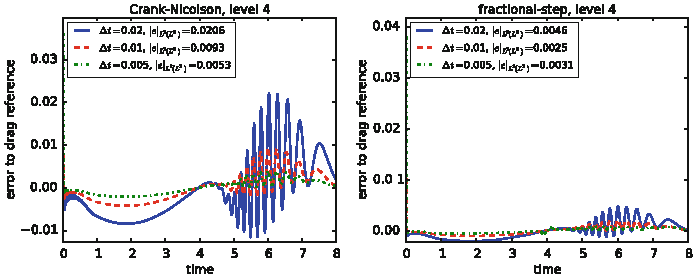
\includegraphics[width=\linewidth]{figures/Chapter_07/Fig_7_04__PDFp412__Bookp402.pdf}
\captionof{figure}{例题\hyperref[ex:time-dependent-accuracy]{7.58}:阻力系数相对于参考曲线的误差;$Q_2/P_1^{\mathrm{disc}}$ 元对;左:Crank--Nicolson 格式,右:分步 $\theta$-格式.}
\label{fig:time-dependent-drag-error-second-order}
\end{elegantfigure}

\begin{elegantfigure}[\linewidth]
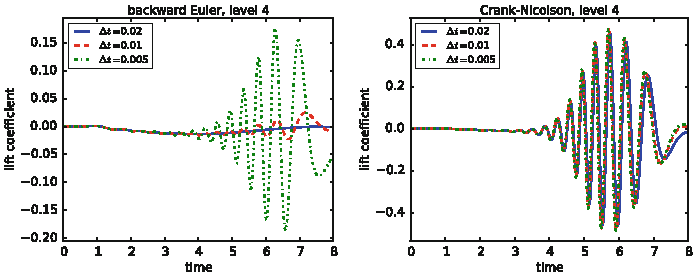
\includegraphics[width=\linewidth]{figures/Chapter_07/Fig_7_05__PDFp412__Bookp402.pdf}
\captionof{figure}{例题\hyperref[ex:time-dependent-accuracy]{7.58}:升力系数随时间的变化;$Q_2/P_1^{\mathrm{disc}}$ 元对;左:后向 Euler 格式,右:Crank--Nicolson 格式.注意两图的尺度不同.}
\label{fig:time-dependent-lift-evolution}
\end{elegantfigure}

升力系数的时间变化(图\hyperref[fig:time-dependent-lift-evolution]{7.5})表明,当时间步长不小于 $\Delta t=0.005$ 时,后向 Euler 格式甚至不能正确预测涡脱落.总的来说,对于空间误差并非占主导的问题,本例展示了高阶空间离散与一阶、二阶时间离散格式结合时,在定性结果上的差异.

\begin{elegantfigure}[\linewidth]
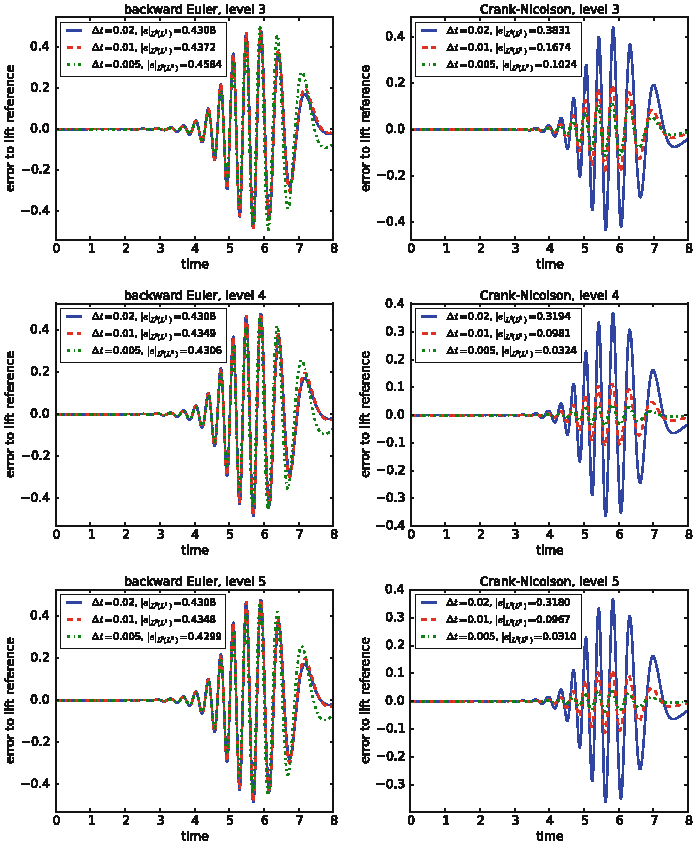
\includegraphics[width=\linewidth]{figures/Chapter_07/Fig_7_06__PDFp413__Bookp403.pdf}
\captionof{figure}{例题\hyperref[ex:time-dependent-accuracy]{7.58}:升力系数相对于图\hyperref[fig:appendix-d-10]{D.10}中参考曲线的误差;$Q_2/P_1^{\mathrm{disc}}$ 元对,第 3--5 层(自上而下);左:后向 Euler 格式,右:Crank--Nicolson 格式.两侧均比较了不同的时间步长.}
\label{fig:time-dependent-lift-error}
\end{elegantfigure}

对于二阶格式,减小时间步长带来的误差下降同样十分明显.二阶时间格式的结果可在图\hyperref[fig:time-dependent-drag-error-second-order]{7.4}、图\hyperref[fig:time-dependent-lift-error-second-order]{7.7}和图\hyperref[fig:time-dependent-pressure-error]{7.8}中比较.尽管 Crank--Nicolson 格式和分步 $\theta$-格式具有相同的阶数,仍可观察到,分步 $\theta$-格式计算得到的各系数精确得多.不过,笔记\hyperref[note:theta-scheme-experience]{7.59}将指出,采用分步 $\theta$-格式模拟流动的计算代价(耗时)通常是 Crank--Nicolson 格式的两到三倍.

\begin{elegantfigure}[\linewidth]
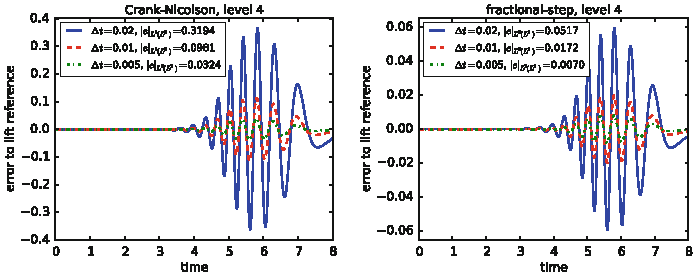
\includegraphics[width=\linewidth]{figures/Chapter_07/Fig_7_07__PDFp414__Bookp404.pdf}
\captionof{figure}{例题\hyperref[ex:time-dependent-accuracy]{7.58}:升力系数相对于图\hyperref[fig:appendix-d-10]{D.10}中参考曲线的误差;$Q_2/P_1^{\mathrm{disc}}$ 元对;左:Crank--Nicolson 格式,右:分步 $\theta$-格式.注意两图的尺度不同.}
\label{fig:time-dependent-lift-error-second-order}
\end{elegantfigure}

\begin{elegantfigure}[\linewidth]
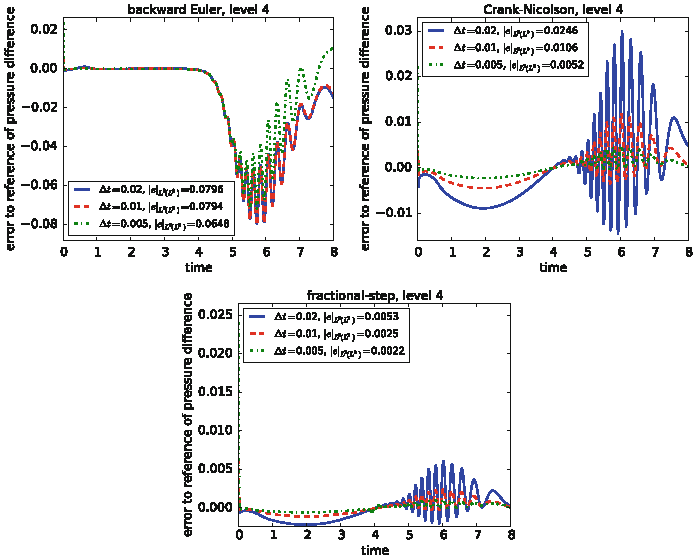
\includegraphics[width=\linewidth]{figures/Chapter_07/Fig_7_08__PDFp414__Bookp404.pdf}
\captionof{figure}{例题\hyperref[ex:time-dependent-accuracy]{7.58}:圆柱前后压差相对于图\hyperref[fig:appendix-d-10]{D.10}中参考曲线的误差;$Q_2/P_1^{\mathrm{disc}}$ 元对;后向 Euler、Crank--Nicolson 和分步 $\theta$-格式的结果按从左到右、从上到下排列.}
\label{fig:time-dependent-pressure-error}
\end{elegantfigure}

在每个离散时刻求解非线性问题时,停止准则的选择颇为微妙.若准则过严,各离散时刻的求解可能耗时很长,从而显著增加总计算时间,但预期可以得到精确结果.相反,采用较宽松的准则可能大幅加快模拟;然而,某些离散时刻的解可能相当不准确,使整体误差明显增大,见图\hyperref[fig:time-dependent-stopping-tolerance]{7.9}.

\begin{elegantfigure}[\linewidth]
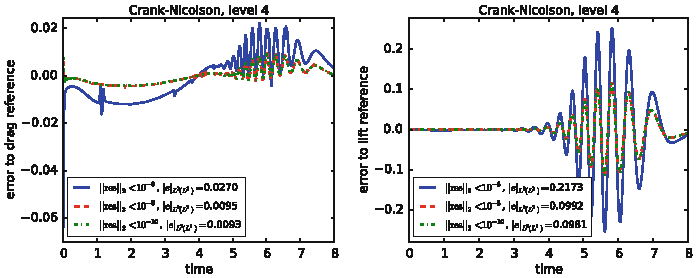
\includegraphics[width=\linewidth]{figures/Chapter_07/Fig_7_09__PDFp415__Bookp405.pdf}
\captionof{figure}{例题\hyperref[ex:time-dependent-accuracy]{7.58}:各离散时刻 Picard 迭代的停止准则对计算精度的影响;$Q_2/P_1^{\mathrm{disc}}$ 元对,Crank--Nicolson 格式,$\Delta t=0.01$.}
\label{fig:time-dependent-stopping-tolerance}
\end{elegantfigure}

图\hyperref[fig:time-dependent-stopping-tolerance]{7.9}显示,与残量向量欧几里得范数不超过 $10^{-6}$ 相比,将其作为停止准则并要求范数不超过 $10^{-8}$,精度会明显提高.据观察,容差取 $10^{-8}$ 时的计算时间约为容差取 $10^{-6}$ 时的 $2.5$ 倍.将容差进一步减小至 $10^{-10}$,相较于 $10^{-8}$ 并不能明显提高精度,但计算时间又增加了约 $2.8$ 倍.何为“严格”或“宽松”的停止准则,取决于具体问题和所用方法.
\index{停止准则}
\end{example}

\begin{note}[Navier--Stokes 方程隐式 $\theta$-格式的数值经验]
\label{note:theta-scheme-experience}
Crank--Nicolson 格式和分步 $\theta$-格式已在 Navier--Stokes 方程中得到充分检验和比较;综述可参见 \textcite{Emmrich2001}.Crank--Nicolson 格式是 A-稳定的,而分步 $\theta$-格式甚至具有强 A-稳定性.这意味着,当初始数据或边界条件不光滑时,Crank--Nicolson 格式可能引起数值振荡;只有采用足够小的时间步,这些振荡才会衰减.与分步 $\theta$-格式相比,为保证 Crank--Nicolson 格式的稳健性,可能需要采用更小的时间步.

二维 Navier--Stokes 方程的数值试验\parencite{JohnRang2010,JohnMatthiesRang2006a}表明,分步 $\theta$-格式所得结果通常比 Crank--Nicolson 格式略精确.不过,分步 $\theta$-格式的计算时间通常是 Crank--Nicolson 格式的两到三倍.总的来说,从单位 CPU 时间所能获得的精度来看,\textcite{JohnRang2010}的结果图中 Crank--Nicolson 格式略占优势.
\index{Crank--Nicolson 格式}
\end{note}

\begin{note}[实现]
\label{note:theta-scheme-implementation}
有限元 $\theta$-格式的基本实现步骤与 Stokes 方程和 Oseen 方程相同,参见第\hyperref[sec:stokes-fem-implementation]{4.3 节}和笔记\hyperref[note:oseen-fem-implementation]{5.19}.表示时间导数离散所需的矩阵只有质量矩阵
\begin{equation}\label{eq:theta-temporal-mass-matrix}
  (M)_{ij}=(\varphi_j^h,\varphi_i^h)_K,\qquad
  i,j=1,\ldots,3N_v.
\end{equation}

对于 Picard 迭代系统\hyperref[eq:general-theta-picard]{(7.85)},若黏性项采用梯度形式,对流项采用对流形式、散度形式或斜对称形式,则代数系统的矩阵为
\[
\resizebox{\linewidth}{!}{$\displaystyle
\begin{pmatrix}
M&0&0&0\\
0&M&0&0\\
0&0&M&0\\
0&0&0&0
\end{pmatrix}
+\Delta t_{n+1}
\begin{pmatrix}
\theta_1A_{11}(\bm{u}_{k+1}^{(m)})&0&0&
\dfrac{\Delta t_{k+1}}{\Delta t_{n+1}}B_1^{\mathsf T}\\
0&\theta_1A_{11}(\bm{u}_{k+1}^{(m)})&0&
\dfrac{\Delta t_{k+1}}{\Delta t_{n+1}}B_2^{\mathsf T}\\
0&0&\theta_1A_{11}(\bm{u}_{k+1}^{(m)})&
\dfrac{\Delta t_{k+1}}{\Delta t_{n+1}}B_3^{\mathsf T}\\
\dfrac{\Delta t_{k+1}}{\Delta t_{n+1}}B_1&
\dfrac{\Delta t_{k+1}}{\Delta t_{n+1}}B_2&
\dfrac{\Delta t_{k+1}}{\Delta t_{n+1}}B_3&0
\end{pmatrix}.
$}
\]
式\hyperref[eq:general-theta-picard]{(7.85)}右端含 $\theta_2$ 的项具有如下矩阵形式:
\begin{equation}\label{eq:picard-explicit-rhs-matrix}
\begin{aligned}
  -\theta_2\Delta t_{n+1}
  \begin{pmatrix}
    A_{11}(\bm{u}_k)&0&0&0\\
    0&A_{11}(\bm{u}_k)&0&0\\
    0&0&A_{11}(\bm{u}_k)&0\\
    0&0&0&0
  \end{pmatrix}
  \begin{pmatrix}\bm{u}_k\\0\end{pmatrix}.
\end{aligned}
\end{equation}
这里,$A_{11}(\bm{u}_k)$ 是在离散时刻 $t_k$ 的 Picard 迭代中最后一次组装得到的矩阵.因此,计算式\hyperref[eq:picard-explicit-rhs-matrix]{(7.88)}只需进行一次矩阵--向量乘法.
\end{note}

\begin{note}[半隐式方法(IMEX 格式)]
\label{note:imex-schemes}\label{note:oseen-semi-implicit}
一种常用方法是采用半隐式格式,即 IMEX(implicit-explicit,隐式--显式)格式.它避免在每个离散时刻求解非线性问题,因此相较于全隐式格式,采用 IMEX 格式进行模拟有望减少计算耗时.

在这类格式中,将一般格式\hyperref[eq:general-theta-scheme]{(7.83)}中出现的非线性项 $(\bm{u}_{k+1}\cdot\nabla)\bm{u}_{k+1}$ 替换为 $(\bm{u}_{\mathrm{prev}}\cdot\nabla)\bm{u}_{k+1}$,其中 $\bm{u}_{\mathrm{prev}}$ 可由已经计算出的解得到.最简单的取法是令 $\bm{u}_{\mathrm{prev}}=\bm{u}_k$,但也常采用前两个时间步的解作线性外推,即
\begin{equation}\label{eq:linear-velocity-extrapolation}
  \bm{u}_{\mathrm{prev}}
  =\frac{\Delta t_{k+1}}{\Delta t_k}
    (\bm{u}_k-\bm{u}_{k-1})+\bm{u}_k.
\end{equation}
\index{IMEX 格式}

当 $\theta=0.5$ 时,这一线性外推(linear extrapolation)所得到的格式与 \textcite{Ingram2013a} 提出并研究的稳定化外推 Crank--Nicolson 格式 CNLE(stab) 类似.对于等时间步长,该文中的对流项为
\begin{equation}\label{eq:cnle-stabilized-convective-term}
\begin{aligned}
  \frac{1}{4}\Delta t\Bigl[
    &(((2\bm{u}_n+\bm{u}_{n-1}-\bm{u}_{n-2})
       \cdot\nabla)\bm{u}_{n+1},\bm{v})\\
    &+(( (2\bm{u}_n+\bm{u}_{n-1}-\bm{u}_{n-2})
       \cdot\nabla)\bm{u}_{n},\bm{v})
  \Bigr].
\end{aligned}
\end{equation}
而采用外推式\hyperref[eq:linear-velocity-extrapolation]{(7.89)}时,所得对流项为
\begin{equation}\label{eq:imex-cnle-convective-term}
\begin{aligned}
  \frac{1}{2}\Delta t\Bigl[
    &(((2\bm{u}_n-\bm{u}_{n-1})
       \cdot\nabla)\bm{u}_{n+1},\bm{v})\\
    &+(( (2\bm{u}_{n-1}-\bm{u}_{n-2})
       \cdot\nabla)\bm{u}_{n},\bm{v})
  \Bigr].
\end{aligned}
\end{equation}
式\hyperref[eq:cnle-stabilized-convective-term]{(7.90)}和式\hyperref[eq:imex-cnle-convective-term]{(7.91)}中的第二项均出现在时间 $t_{n+1}$ 对应方程的右端.注意,
\[
  \frac{2}{4}(2\bm{u}_n+\bm{u}_{n-1}-\bm{u}_{n-2})
  =\frac{1}{2}(2\bm{u}_n-\bm{u}_{n-1})
   +\frac{1}{2}(2\bm{u}_{n-1}-\bm{u}_{n-2}),
\]
因此,式\hyperref[eq:cnle-stabilized-convective-term]{(7.90)}和式\hyperref[eq:imex-cnle-convective-term]{(7.91)}将外推速度场以不同方式分配给离散时刻 $t_{n+1}$ 和 $t_n$ 对应的项.式\hyperref[eq:imex-cnle-convective-term]{(7.91)}使得在 $t_{n+1}$ 时计算方程右端时,可以使用在 $t_n$ 组装的矩阵,参见笔记\hyperref[note:theta-scheme-implementation]{7.60}.
\end{note}

\begin{example}[\enspace IMEX 格式]
\label{ex:imex-schemes-cylinder}
为展示 IMEX 格式的性能,考虑具有定常入口流的二维绕圆柱流动,即例题\hyperref[ex:appendix-d-8]{D.8}.模拟采用 $Q_2/P_1^{\mathrm{disc}}$ 元对;初始网格见图\hyperref[fig:steady-ns-cylinder-initial-grids]{6.5},自由度数见表\hyperref[tab:time-dependent-cylinder-dofs]{7.4}.Crank--Nicolson 格式的时间步长取 $\Delta t=0.005$.IMEX 格式分别采用常值外推 $\bm{u}_{\mathrm{prev}}=\bm{u}_n$ 和线性外推式\hyperref[eq:imex-cnle-convective-term]{(7.91)}.

图\hyperref[fig:imex-cylinder-quantities]{7.10}给出了第 4 层网格上的结果;第 3 层和第 5 层上的结果在定性上相同.可以看到,采用常值外推的 IMEX 格式精度较差,例如阻力系数和升力系数的最大值都明显偏大.\textcite{CaiazzoIliescuJohnSchyschlowa2014}在后向 Euler 格式配合常值外推时也观察到相同现象.相反,IMEX 格式采用线性外推时,结果精度几乎与全隐式格式相同.

\textcite{TabataTagami2000}对后向 Euler 格式配合常值外推时计算得到的阻力系数和升力系数作了数值分析.该分析假定 Navier--Stokes 方程的解具有足够的正则性.然而,重要量为阻力和升力的绕物体流动问题,其计算区域通常不是凸域,因此这一假设是否成立并不明确.

效率提升幅度取决于许多因素,例如具体问题、所用求解器和实现细节.对于本例给出的数值结果,IMEX 格式采用稀疏直接求解器 UMFPACK,参见 \textcite{Davis2004};该求解器用于 IMEX 格式的情况亦见第\hyperref[note:chapter9-solver-choice]{9.5 条笔记}.

\begin{elegantfigure}[\linewidth]
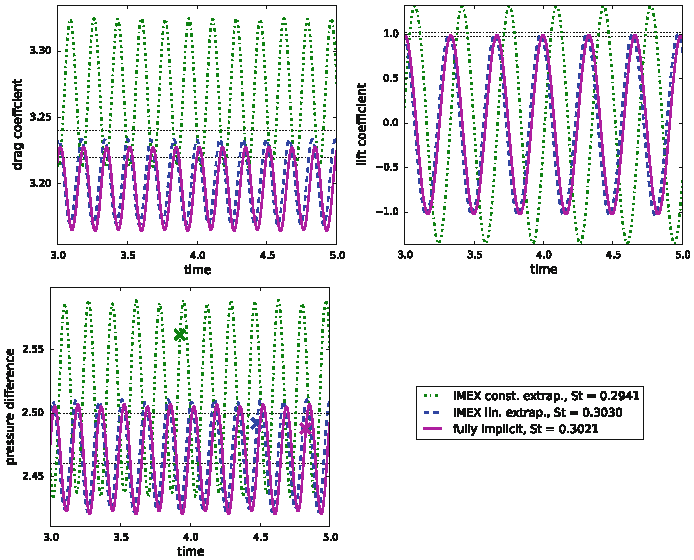
\includegraphics[width=\linewidth]{figures/Chapter_07/Fig_7_10__PDFp418__Bookp408.pdf}
\captionof{figure}{例题\hyperref[ex:imex-schemes-cylinder]{7.62}:感兴趣量.表\hyperref[tab:appendix-d-2]{D.2}中的参考区间以虚线表示;叉号表示周期的中点.Strouhal 数的参考区间为 $[0.295,0.305]$.}
\label{fig:imex-cylinder-quantities}
\end{elegantfigure}

全隐式格式则采用 Picard 迭代,并对线性系统作非精确求解:残量向量的欧几里得范数每次缩小至原来的十分之一,Picard 迭代的停止准则为该范数小于 $10^{-8}$.求解器采用带耦合多重网格预条件子的 FGMRES 方法,见第\hyperref[subsec:chapter9-iterative-solvers]{9.2.2 节}.本例中,IMEX 格式在第 3、4、5 层上的模拟分别快约 $40$ 倍、$10$ 倍和 $2.25$ 倍.网格越细,效率提升幅度越小,因为细化网格时,迭代求解器的扩展性优于稀疏直接求解器.
\end{example}

\begin{note}[自适应时间步长控制]
\label{note:adaptive-time-step-control}
常微分方程数值模拟中的自适应时间步长控制(adaptive time-step control)已有成熟方法,例如参见 \textcite[第 II.4 节]{HairerNoersettWanner1993}.这些方法通过比较由不同阶数的方法得到的两个解,并利用所谓的控制器(controller)确定下一时间步的长度.若条件允许,可采用所谓的嵌入格式(embedded scheme),以较低计算代价求得比原时间离散格式低一阶的近似解.然而,$\theta$-格式这一类方法没有嵌入格式,因此需要采用其他自适应时间步长控制方法.
\index{自适应时间步长控制}

\textcite{Turek1999}提出通过比较分步 $\theta$-格式和 Crank--Nicolson 格式的结果来控制时间步长.这两种格式的误差展开式首项具有不同的常数;利用该差异和两种格式所得解之间的差异,可以预测合适的时间步长.这种方法的主要缺点是计算代价高:Crank--Nicolson 格式这一步只用于确定下一时间步的长度,而其计算成本不可忽略,因此会显著增加每个时间步的开销.\textcite{KayGreshoGriffithsSilvester2010}提出了类似但代价较低的方法,即比较 Crank--Nicolson 格式与二阶显式 Adams--Bashforth 方法所得的速度解来控制步长.另一种更具启发性的做法,是在某个范数下监测已计算解的变化,并据此调整时间步长,例如参见 \textcite{BerroneMarro2009}.
\end{note}
\subsection{其他格式}\label{subsec:time-dependent-other-schemes}

\begin{note}[二阶后向差分公式(BDF2)]
\label{note:bdf2-scheme}
将二阶后向差分公式(backward differentiation formula of order two,BDF2)用于 Navier--Stokes 方程组\cref{eq:time-dependent-ns-strong},得到
\begin{equation}\label{eq:bdf2-time-discretization}
\begin{aligned}
  &\frac32\bm{u}_{n+1}
   +\Delta t_{n+1}\Bigl[-\nu\Delta\bm{u}_{n+1}
       +(\bm{u}_{n+1}\cdot\nabla)\bm{u}_{n+1}\Bigr]
   +\Delta t_{n+1}\nabla p_{n+1}\\
  &=2\bm{u}_n-\frac12\bm{u}_{n-1}
    -\Delta t_{n+1}\Bigl[-\nu\Delta\bm{u}_n
       +(\bm{u}_n\cdot\nabla)\bm{u}_n\Bigr]
    +\Delta t_{n+1}\bm{f}_{n+1},\\
  0&=\Delta t_{n+1}\nabla\cdot\bm{u}_{n+1},
\end{aligned}
\end{equation}
其中 $n\ge2$.BDF2 是二阶格式,并且具有强 A-稳定性.因此,与 Crank--Nicolson 格式\hyperref[ex:time-dependent-crank-nicolson]{(见例题 7.49)}相比,它阶数相同、稳定性更强,但需要保存 $\bm{u}_{n-1}$.由于阶数较高且稳定,BDF2 是一种常用格式;例如,它是软件包 deal.II 中的标准时间离散格式,见\textcite{BangerthHartmannKanschat2007}.
\index{BDF2}
\end{note}

\begin{note}[高阶方法]
\label{note:time-dependent-higher-order-schemes}
\textcite{JohnMatthiesRang2006a} 比较了三阶、分别具有 $s=3$ 或 $s=4$ 个阶段的 Rosenbrock 方法与 $\theta$-格式.这些方法是线性隐式 Runge--Kutta 格式.每个离散时刻都要用同一个系统矩阵求解 $s$ 个线性鞍点问题.Rosenbrock 方法可以利用嵌入格式有效地控制时间步长.对于\textcite{JohnMatthiesRang2006a} 所研究的二维问题,Rosenbrock 方法所得数值解通常比 $\theta$-格式精确得多;但采用 $\theta$-格式的模拟明显更高效.\textcite{JohnRang2010} 还在二维绕圆柱流动问题(见例题\hyperref[ex:appendix-d-9]{D.9})上研究并比较了最高四阶的 Rosenbrock 方法、对角隐式 Runge--Kutta 方法(diagonally implicit Runge--Kutta,DIRK)与 $\theta$-格式.所有高阶格式,即阶数至少为三的格式,都可以通过嵌入方法自适应地控制时间步长.若采用时间步长控制,则许多高阶方法在精度与 CPU 时间之比方面明显优于 $\theta$-格式.

尽管如此,目前高阶时间推进格式似乎还不常用.
\index{Rosenbrock 方法}
\index{Runge--Kutta 方法!对角隐式}
\end{note}

\section{有限元误差分析:完全离散情形}\label{sec:time-dependent-fem-fully-discrete}

\begin{note}[与时间连续情形的比较及本节内容]
\label{note:fully-discrete-error-analysis-content}
完全离散 Navier--Stokes 方程组的数值分析与第\hyperref[sec:time-dependent-fem-continuous]{7.2 节}介绍的时间连续情形相似.不过,对时间导数作离散会引入一致性误差,其估计将在引理\hyperref[lem:temporal-derivative-consistency]{7.67}中给出.在完全离散情形中,公式里会出现对离散时刻求和,而不再是时空范数.因此,与时间连续情形相比,论述不那么紧凑,处理也略为繁琐.

本节以时间上采用后向 Euler 格式、空间上采用 Galerkin 有限元方法为例,介绍完全离散情形的分析.为简洁起见,误差分析仅给出速度的估计.
\end{note}

\begin{lemma}[时间导数离散的一致性误差]
\label{lem:temporal-derivative-consistency}
设 $v,\partial_t v,\partial_{tt}v\in L^2(t_n,t_{n+1};L^2(\Omega))$,则
\begin{equation}\label{eq:backward-difference-consistency}
  \left\|\partial_t v_{n+1}
      -\frac{v_{n+1}-v_n}{\Delta t}\right\|_{L^2(\Omega)}^2
   \le \Delta t\,\|\partial_{tt}v\|_{L^2(t_n,t_{n+1};L^2(\Omega))}^2.
\end{equation}
若进一步有 $\partial_{ttt}v\in L^2(t_n,t_{n+1};L^2(\Omega))$,则
\begin{equation}\label{eq:midpoint-difference-consistency}
  \left\|\partial_t v_{n+1/2}
      -\frac{v_{n+1}-v_n}{\Delta t}\right\|_{L^2(\Omega)}^2
   \le \Delta t^3\,\|\partial_{ttt}v\|_{L^2(t_n,t_{n+1};L^2(\Omega))}^2.
\end{equation}
\end{lemma}

\begin{proof}
对带积分余项的 Taylor 公式作分部积分,也可得到
\[
  v_n=v_{n+1}-\Delta t\,\partial_t v_{n+1}
       +\int_{t_n}^{t_{n+1}}(t-t_n)\,\partial_{tt}v\,\mathrm{d}t,
\]
这等价于
\[
  \partial_t v_{n+1}-\frac{v_{n+1}-v_n}{\Delta t}
    =\frac1{\Delta t}\int_{t_n}^{t_{n+1}}
       (t-t_n)\,\partial_{tt}v\,\mathrm{d}t.
\]
利用 Cauchy--Schwarz 不等式\hyperref[eq:appendix-a-10]{(A.10)},注意到其中一个因子与空间变量无关,并应用 Fubini 定理,可得
\[
\begin{aligned}
 &\left\|\partial_t v_{n+1}
       -\frac{v_{n+1}-v_n}{\Delta t}\right\|_{L^2(\Omega)}^2\\
 &\quad\le \frac1{\Delta t^2}
   \left(\int_{t_n}^{t_{n+1}}(t-t_n)^2\,\mathrm{d}t\right)
   \left(\int_{t_n}^{t_{n+1}}\int_\Omega
       (\partial_{tt}v)^2\,\mathrm{d}x\,\mathrm{d}t\right)\\
 &\quad=\frac{\Delta t}{3}
       \|\partial_{tt}v\|_{L^2(t_n,t_{n+1};L^2(\Omega))}^2
   \le \Delta t\,\|\partial_{tt}v\|_{L^2(t_n,t_{n+1};L^2(\Omega))}^2,
\end{aligned}
\]
故得\cref{eq:backward-difference-consistency}.这里为简洁起见,将因子 $1/3$ 以 $1$ 代替.

\cref{eq:midpoint-difference-consistency} 的证明方法相同.对任意 $\theta\in[0,1]$ 作 Taylor 展开,或连续分部积分,可得
\[
\begin{aligned}
 v_n={}&v_{n+\theta}-\theta\Delta t\,\partial_t v_{n+\theta}
       +\frac{\theta^2}{2}\Delta t^2\partial_{tt}v_{n+\theta}\\
      &\quad+\frac12\int_{t_n}^{t_{n+\theta}}
          (t_n-t)^2\partial_{ttt}v\,\mathrm{d}t,\\
 v_{n+1}={}&v_{n+\theta}+(1-\theta)\Delta t\,\partial_t v_{n+\theta}
       +\frac{(1-\theta)^2}{2}\Delta t^2\partial_{tt}v_{n+\theta}\\
      &\quad+\frac12\int_{t_{n+\theta}}^{t_{n+1}}
          (t_{n+1}-t)^2\partial_{ttt}v\,\mathrm{d}t.
\end{aligned}
\]
将第二式从第一式中相减并整理,得到
\[
\begin{aligned}
 \partial_t v_{n+\theta}
   ={}&\frac{v_{n+1}-v_n}{\Delta t}
      +\frac{\Delta t}{2}\bigl(\theta^2-(1-\theta)^2\bigr)
          \partial_{tt}v_{n+\theta}\\
     &-\frac1{2\Delta t}\int_{t_n}^{t_{n+\theta}}
          (t_n-t)^2\partial_{ttt}v\,\mathrm{d}t
      \\[-1mm]
     &-\frac1{2\Delta t}\int_{t_{n+\theta}}^{t_{n+1}}
          (t_{n+1}-t)^2\partial_{ttt}v\,\mathrm{d}t.
\end{aligned}
\]
含 $\partial_{tt}v_{n+\theta}$ 的项仅当 $\theta=1/2$ 时才消失.取 $\theta=1/2$,并像证明\cref{eq:backward-difference-consistency} 那样处理,可得
\[
\begin{aligned}
 &\left\|\partial_t v_{n+1/2}
       -\frac{v_{n+1}-v_n}{\Delta t}\right\|_{L^2(\Omega)}^2\\
 &\quad\le\frac1{4\Delta t^2}\Biggl[
   \left(\int_{t_n}^{t_{n+1/2}}(t_n-t)^4\,\mathrm{d}t\right)
   \left(\int_\Omega\int_{t_n}^{t_{n+1/2}}
       (\partial_{ttt}v)^2\,\mathrm{d}t\,\mathrm{d}x\right)\\
 &\qquad\qquad+
   \left(\int_{t_{n+1/2}}^{t_{n+1}}(t_{n+1}-t)^4\,\mathrm{d}t\right)
   \left(\int_\Omega\int_{t_{n+1/2}}^{t_{n+1}}
       (\partial_{ttt}v)^2\,\mathrm{d}t\,\mathrm{d}x\right)
   \Biggr],
\end{aligned}
\]
直接计算即得\cref{eq:midpoint-difference-consistency}.
\end{proof}

\begin{note}[后向 Euler 格式]
\label{note:backward-euler-scheme}
等步长的后向 Euler 格式如下:给定 $\bm{f}_{n+1}\in V'$ 和 $\bm{u}_n^h\in V^h$,通过求解下列问题计算 $(\bm{u}_{n+1}^h,p_{n+1}^h)\in V^h\times Q^h$,其中 $n=0,1,2,\ldots$:
\begin{equation}\label{eq:fully-discrete-backward-euler}
\begin{aligned}
 &\frac1{\Delta t}(\bm{u}_{n+1}^h-\bm{u}_n^h,\bm{v}^h)
   +\nu(\nabla\bm{u}_{n+1}^h,\nabla\bm{v}^h)
   +n_{\mathrm{skew}}(\bm{u}_{n+1}^h,\bm{u}_{n+1}^h,\bm{v}^h)\\
 &\quad-(\nabla\cdot\bm{v}^h,p_{n+1}^h)
       +(\nabla\cdot\bm{u}_{n+1}^h,q^h)
    =\langle\bm{f}_{n+1},\bm{v}^h\rangle_{V',V},\\
 &\hspace{7em}\forall(\bm{v}^h,q^h)\in V^h\times Q^h.
\end{aligned}
\end{equation}
初始条件 $\bm{u}_0^h$ 是将 $\bm{u}_0$ 插值或投影到有限元空间所得的函数,例如 Lagrange 插值或 Stokes 投影\hyperref[eq:stokes-projection-definition]{(4.54)}.
\index{后向 Euler 格式}
\end{note}

\begin{lemma}[有限元解的存在性、唯一性与稳定性]
\label{lem:fully-discrete-backward-euler-existence-stability}
设有限元空间对 $V^h$ 与 $Q^h$ 满足离散 inf-sup 条件\hyperref[eq:discrete-infsup-condition]{(3.51)}.当时间步长足够小时,问题\cref{eq:fully-discrete-backward-euler} 有唯一解.时间步长的限制依赖于网格宽度.

对问题\cref{eq:fully-discrete-backward-euler} 的任意解以及所有 $N\ge0$,均有
\begin{equation}\label{eq:fully-discrete-backward-euler-stability}
  \begin{aligned}
    &\|\bm{u}_{N+1}^h\|_{L^2(\Omega)}^2\\
    &+\nu\Delta t\sum_{n=0}^{N}
         \|\nabla\bm{u}_{n+1}^h\|_{L^2(\Omega)}^2\\
    &\le \|\bm{u}_0^h\|_{L^2(\Omega)}^2\\
    &\quad+\frac{\Delta t}{\nu}\sum_{n=0}^{N}
         \|\bm{f}_{n+1}\|_{H^{-1}(\Omega)}^2.
  \end{aligned}
\end{equation}
\end{lemma}

\begin{proof}
先证明稳定性估计\cref{eq:fully-discrete-backward-euler-stability},因为随后证明解的存在性和唯一性时会用到该估计.

\textit{稳定性.} 按通常方法,在问题\cref{eq:fully-discrete-backward-euler} 中取任意解作为检验函数,即令 $(\bm{v}^h,q^h)=(\bm{u}_{n+1}^h,p_{n+1}^h)$.由对流项的斜对称性\hyperref[eq:steady-ns-nskew-definition]{(6.25)},有
$n_{\mathrm{skew}}(\bm{u}_{n+1}^h,\bm{u}_{n+1}^h,\bm{u}_{n+1}^h)=0$,因而
\begin{equation}\label{eq:fully-discrete-backward-euler-energy}
  \frac1{\Delta t}(\bm{u}_{n+1}^h-\bm{u}_n^h,\bm{u}_{n+1}^h)
   +\nu\|\nabla\bm{u}_{n+1}^h\|_{L^2(\Omega)}^2
    =\langle\bm{f}_{n+1},\bm{u}_{n+1}^h\rangle_{V',V}.
\end{equation}
类似于实数 $a,b$ 的代数关系
$a^2-ab=\tfrac12\bigl(a^2+(a-b)^2-b^2\bigr)$,有
\begin{equation}\label{eq:backward-euler-time-difference-identity}
\begin{aligned}
 (\bm{u}_{n+1}^h-\bm{u}_n^h,\bm{u}_{n+1}^h)
  =\frac12\Bigl(&\|\bm{u}_{n+1}^h\|_{L^2(\Omega)}^2
       +\|\bm{u}_{n+1}^h-\bm{u}_n^h\|_{L^2(\Omega)}^2\\
       &-\|\bm{u}_n^h\|_{L^2(\Omega)}^2\Bigr).
\end{aligned}
\end{equation}
将\cref{eq:backward-euler-time-difference-identity}代入\cref{eq:fully-discrete-backward-euler-energy},并利用
$\|\bm{u}_{n+1}^h-\bm{u}_n^h\|_{L^2(\Omega)}^2\ge0$,可得
\[
  \|\bm{u}_{n+1}^h\|_{L^2(\Omega)}^2
   +2\nu\Delta t\|\nabla\bm{u}_{n+1}^h\|_{L^2(\Omega)}^2
  \le \|\bm{u}_n^h\|_{L^2(\Omega)}^2
     +2\Delta t\langle\bm{f}_{n+1},\bm{u}_{n+1}^h\rangle_{V',V}.
\]
对偶配对估计和 Young 不等式\hyperref[eq:appendix-a-5]{(A.5)}给出
\[
  \|\bm{u}_{n+1}^h\|_{L^2(\Omega)}^2
   +\nu\Delta t\|\nabla\bm{u}_{n+1}^h\|_{L^2(\Omega)}^2
  \le \|\bm{u}_n^h\|_{L^2(\Omega)}^2
     +\frac{\Delta t}{\nu}
       \|\bm{f}_{n+1}\|_{H^{-1}(\Omega)}^2.
\]
从 $n=0$ 到 $N$ 求和,并注意两边的第一项形成望远镜求和,即得稳定性估计\cref{eq:fully-discrete-backward-euler-stability}.

\textit{解的存在性与唯一性.} 后向 Euler 格式\cref{eq:fully-discrete-backward-euler} 在每个离散时刻都要求解一个非线性离散问题,其形式与定常 Navier--Stokes 方程组相似,只是多了由时间离散产生的项.解的存在性与唯一性可用与定常 Navier--Stokes 方程组相同的方法证明,参见定理\hyperref[thm:steady-ns-existence]{6.17}的证明.考虑 Oseen 型问题:给定 $\bm{f}_{n+1}\in V'$ 以及 $\bm{b}^h,\bm{u}_n^h\in V_{\mathrm{div}}^h$,求 $\bm{u}^h\in V_{\mathrm{div}}^h$,使得
\begin{equation}\label{eq:fully-discrete-backward-euler-oseen}
  \begin{aligned}
   &\frac1{\Delta t}(\bm{u}^h,\bm{v}^h)
      +\nu(\nabla\bm{u}^h,\nabla\bm{v}^h)
      +n_{\mathrm{skew}}(\bm{b}^h,\bm{u}^h,\bm{v}^h)\\
   &\quad=\frac1{\Delta t}(\bm{u}_n^h,\bm{v}^h)
      +\langle\bm{f}_{n+1},\bm{v}^h\rangle_{V',V},\\
   &\hspace{8em}\forall\bm{v}^h\in V_{\mathrm{div}}^h.
  \end{aligned}
\end{equation}
由此定义算子
\[
  \mathcal N_{\mathrm{conv}}^h:V_{\mathrm{div}}^h\to V_{\mathrm{div}}^h,
  \qquad \bm{b}^h\mapsto\bm{u}^h.
\]
问题\cref{eq:fully-discrete-backward-euler-oseen} 对每个给定的 $\bm{b}^h$ 都有唯一解;这一点由 Lax--Milgram 定理得到,细节参见引理\hyperref[lem:imex-euler-existence-uniqueness-stability]{7.77}的证明.算子 $\mathcal N_{\mathrm{conv}}^h$ 的每个不动点都是后向 Euler 问题\cref{eq:fully-discrete-backward-euler} 在时刻 $t_{n+1}$ 的一个速度解.由于当检验函数为 $\bm{v}^h=\bm{u}^h$ 时,对流项消失,仿照稳定性估计的第一部分可得
\begin{equation}\label{eq:fully-discrete-backward-euler-oseen-stability}
  \|\bm{u}^h\|_{L^2(\Omega)}^2
   +\nu\Delta t\|\nabla\bm{u}^h\|_{L^2(\Omega)}^2
  \le \|\bm{u}_n^h\|_{L^2(\Omega)}^2
     +\frac{\Delta t}{\nu}\|\bm{f}_{n+1}\|_{H^{-1}(\Omega)}^2.
\end{equation}
由此可见,算子 $\mathcal N_{\mathrm{conv}}^h$ 关于 $\bm{b}^h$ 有界,且界与 $\bm{b}^h$ 无关:
\[
\begin{aligned}
 \|\mathcal N_{\mathrm{conv}}^h\|
  &=\sup_{\substack{\bm{b}^h\in V_{\mathrm{div}}^h\\
                     \|\bm{b}^h\|_V=1}}
       \|\mathcal N_{\mathrm{conv}}^h\bm{b}^h\|_V
   =\sup_{\substack{\bm{b}^h\in V_{\mathrm{div}}^h\\
                     \|\bm{b}^h\|_V=1}}\|\bm{u}^h\|_V\\
  &\le\left(\frac1{\nu\Delta t}\|\bm{u}_n^h\|_{L^2(\Omega)}^2
       +\frac1{\nu^2}\|\bm{f}_{n+1}\|_{H^{-1}(\Omega)}^2\right)^{1/2}.
\end{aligned}
\]
在估计\cref{eq:fully-discrete-backward-euler-oseen-stability}左端的第一项中应用逆估计\hyperref[eq:appendix-c-37]{(C.37)},得到
\begin{equation}\label{eq:fully-discrete-backward-euler-inverse-bound}
  \|\nabla\bm{u}^h\|_{L^2(\Omega)}^2
   \le\frac1{C_{\mathrm{inv}}^{-2}h^2+\nu\Delta t}
       \left(\|\bm{u}_n^h\|_{L^2(\Omega)}^2
         +\frac{\Delta t}{\nu}
             \|\bm{f}_{n+1}\|_{H^{-1}(\Omega)}^2\right).
\end{equation}
任取 $\bm{b}_1^h,\bm{b}_2^h\in V_{\mathrm{div}}^h$,令
$\bm{u}_1^h=\mathcal N_{\mathrm{conv}}^h\bm{b}_1^h$、
$\bm{u}_2^h=\mathcal N_{\mathrm{conv}}^h\bm{b}_2^h$,并将相应问题相减.取
$\bm{v}^h=\bm{u}_1^h-\bm{u}_2^h$,可得
\begin{equation}\label{eq:fully-discrete-backward-euler-operator-difference}
\begin{aligned}
 &\frac1{\Delta t}\|\bm{u}_1^h-\bm{u}_2^h\|_{L^2(\Omega)}^2
   +\nu\|\nabla(\bm{u}_1^h-\bm{u}_2^h)\|_{L^2(\Omega)}^2\\
 &\qquad=-n_{\mathrm{skew}}(\bm{b}_1^h-\bm{b}_2^h,
              \bm{u}_1^h,\bm{u}_1^h-\bm{u}_2^h).
\end{aligned}
\end{equation}
对\cref{eq:fully-discrete-backward-euler-operator-difference}左端第一项应用逆估计,并利用对流项估计\hyperref[eq:steady-ns-conv-estimate-29]{(6.29)},得到
\[
\begin{aligned}
 &\left(\frac{C_{\mathrm{inv}}^{-2}h^2}{\Delta t}+\nu\right)
      \|\nabla(\bm{u}_1^h-\bm{u}_2^h)\|_{L^2(\Omega)}^2\\
 &\quad\le N_{\mathrm{div}}^h\|\bm{b}_1^h-\bm{b}_2^h\|_V
      \|\bm{u}_1^h\|_V\\
 &\hspace{8em}\times\|\nabla(\bm{u}_1^h-\bm{u}_2^h)\|_{L^2(\Omega)},
\end{aligned}
\]
其中 $N_{\mathrm{div}}^h$ 由\hyperref[eq:steady-ns-discrete-convection-norm]{(6.57)}定义.再代入\cref{eq:fully-discrete-backward-euler-inverse-bound},可得
\[
\begin{aligned}
 &\|\nabla(\bm{u}_1^h-\bm{u}_2^h)\|_{L^2(\Omega)}\\
 &\quad\le N_{\mathrm{div}}^h\Delta t
       \left(\frac1{C_{\mathrm{inv}}^{-2}h^2+\nu\Delta t}\right)^{3/2}\\
 &\qquad\times\left(\|\bm{u}_n^h\|_{L^2(\Omega)}^2
          +\frac{\Delta t}{\nu}
              \|\bm{f}_{n+1}\|_{H^{-1}(\Omega)}^2\right)^{1/2}\\
 &\qquad\times\|\bm{b}_1^h-\bm{b}_2^h\|_V.
\end{aligned}
\]
当时间步长足够小时,$\|\bm{b}_1^h-\bm{b}_2^h\|_V$ 前的系数小于 $1$.此时由 Banach 不动点定理\hyperref[thm:appendix-a-68]{A.68},问题\cref{eq:fully-discrete-backward-euler} 的速度解存在且唯一.时刻 $t_{n+1}$ 的压力解存在且唯一,则由有限元空间满足离散 inf-sup 条件可知.
\end{proof}

\begin{note}[关于解的存在性与唯一性]
\label{note:fully-discrete-solution-existence-uniqueness}
问题\cref{eq:fully-discrete-backward-euler} 与定常 Navier--Stokes 方程组形式相近.对任意长度的时间步证明解的存在性,可采用与定常 Navier--Stokes 方程组存在性证明相同的方法,参见\textcite[第 15.2 节]{MarionTemam1998}以及定理\hyperref[thm:steady-ns-existence]{6.17}证明中所引的文献.

若对解作更强的正则性假设,则可以证明:当时间步长足够小时,解唯一,且时间步长条件不依赖网格尺寸.例如,假设 $\nabla\bm{u}\in L^\infty(0,T;L^2(\Omega))$,\textcite[式(3.15)]{HeywoodRannacher1990}证明了
$\|\nabla\bm{u}^h\|_{L^\infty(0,T;L^2(\Omega))}<C$,其中常数 $C$ 与 $h$ 无关.将此界代入\cref{eq:fully-discrete-backward-euler-inverse-bound},便得到一个不依赖网格宽度的时间步长条件.

另一种做法是先证明解存在,再在时间步长足够小时证明唯一性.假设有两个解 $\bm{u}_1^h$ 和 $\bm{u}_2^h$,将它们的方程相减,并以两解之差作为检验函数,得到
\begin{equation}\label{eq:fully-discrete-backward-euler-uniqueness}
\begin{aligned}
 &\frac1{\Delta t}\|\bm{u}_1^h-\bm{u}_2^h\|_{L^2(\Omega)}^2
    +\nu\|\nabla(\bm{u}_1^h-\bm{u}_2^h)\|_{L^2(\Omega)}^2\\
 &=-n_{\mathrm{skew}}(\bm{u}_1^h,\bm{u}_1^h,
                   \bm{u}_1^h-\bm{u}_2^h)
    +n_{\mathrm{skew}}(\bm{u}_2^h,\bm{u}_1^h,
                   \bm{u}_1^h-\bm{u}_2^h)\\
 &=n_{\mathrm{conv}}(\bm{u}_1^h-\bm{u}_2^h,\bm{u}_1^h,
                    \bm{u}_1^h-\bm{u}_2^h)\\
 &\quad+\frac12\bigl(\nabla\cdot(\bm{u}_1^h-\bm{u}_2^h),
                \bm{u}_1^h\cdot(\bm{u}_1^h-\bm{u}_2^h)\bigr).
\end{aligned}
\end{equation}
这里用到了斜对称型的定义\hyperref[eq:steady-ns-nskew-definition]{(6.25)}和\hyperref[eq:steady-ns-conv-form-4]{(6.13)}.若假设 $\bm{u}_1^h\in L^\infty((0,T);L^\infty(\Omega))$,则\cref{eq:fully-discrete-backward-euler-uniqueness}右端可估计为
\[
  \frac32\|\bm{u}_1^h\|_{L^\infty(\Omega)}
       \|\bm{u}_1^h-\bm{u}_2^h\|_{L^2(\Omega)}
       \|\nabla(\bm{u}_1^h-\bm{u}_2^h)\|_{L^2(\Omega)}.
\]
在此假设下,$\|\bm{u}_1^h\|_{L^\infty(\Omega)}$ 可由一个与 $h$ 无关的常数控制,见\textcite[式(2.16)及注记 5.1]{deFrutos2008}.随后应用 Young 不等式\hyperref[eq:appendix-a-5]{(A.5)},可得只有在时间步长足够小时才能成立的不等式;这一时间步长限制不依赖 $h$.
\end{note}

\begin{note}[时空范数的近似]
\label{note:time-space-norm-approximation}
设 $X$ 是赋范空间,范数为 $\|\cdot\|_X$.对 $p\in[1,\infty)$、$0\le t_0<t_N$ 以及 $v\in L^p(t_0,t_N;X)$,函数 $v$ 的范数的 $p$ 次幂为
\begin{equation}\label{eq:time-space-norm-integral}
  \|v\|_{L^p(t_0,t_N;X)}^p
    =\int_{t_0}^{t_N}\|v\|_X^p\,\mathrm{d}t.
\end{equation}
式\cref{eq:time-space-norm-integral}可用复合梯形公式(composite trapezoidal rule)近似.为此,将区间 $[t_0,t_N]$ 划分为长度均为 $\Delta t$ 的子区间.在每个子区间上应用梯形公式
\[
  \int_{t_n}^{t_{n+1}}\|v\|_X^p\,\mathrm{d}t
    \approx\frac{\Delta t}{2}
       \Bigl(\|v(t_{n+1})\|_X^p+\|v(t_n)\|_X^p\Bigr).
\]
将所有子区间上的近似值相加,便得到\cref{eq:time-space-norm-integral}的如下近似:
\[
  \|v\|_{L^p(t_0,t_N;X)}^p
    \approx\Delta t\left(
       \frac{\|v(t_0)\|_X^p}{2}
       +\sum_{n=1}^{N-1}\|v(t_n)\|_X^p
       +\frac{\|v(t_N)\|_X^p}{2}\right).
\]
由此可见,估计\cref{eq:fully-discrete-backward-euler-stability}中的求和项就是复合梯形公式的近似.例如,
\[
  \|\nabla\bm{u}^h\|_{L^2(t_1,t_{N+1};L^2(\Omega))}^2
    \approx\Delta t\sum_{n=0}^{N}
       \|\nabla\bm{u}_{n+1}^h\|_{L^2(\Omega)}^2.
\]
\index{复合梯形公式}
\end{note}

\begin{theorem}[后向 Euler 格式与 Galerkin 有限元方法的速度误差估计]
\label{thm:fully-discrete-backward-euler-velocity-error}\label{thm:time-dependent-fem-fully-discrete-error}
设 $\Omega\subset\mathbb R^d$ 为有界多面体域,$d\in\{2,3\}$,且其边界为 Lipschitz 连续边界.设
$\bm{f}\in L^2(0,T;V')$、$\bm{u}_0\in H_{\mathrm{div}}(\Omega)$、
$\bm{u}_0^h\in V_{\mathrm{div}}^h$,并假设 Navier--Stokes 方程组\cref{eq:time-dependent-ns-weak-first} 的解 $(\bm{u},p)$ 满足
\begin{equation}\label{eq:fully-discrete-backward-euler-error-regularity}
\begin{aligned}
  \partial_{tt}\bm{u}&\in L^2(0,T;H^1(\Omega)),
  &\partial_t\bm{u}&\in L^2(0,T;V'),\\
  \nabla\bm{u}&\in L^4(0,T;L^2(\Omega)),
  &p&\in L^2(0,T;L^2(\Omega)).
\end{aligned}
\end{equation}
以下记 $\bm{u}_n=\bm{u}(t_n)$、$p_n=p(t_n)$.考虑时间上采用后向 Euler 格式、空间上采用 Galerkin 有限元方法的离散\cref{eq:fully-discrete-backward-euler}.设空间对 $V^h\times Q^h$ 满足 inf-sup 条件,时间步长均匀为 $\Delta t$,即 $t_n=n\Delta t$.假设引理\hyperref[lem:fully-discrete-backward-euler-existence-stability]{7.69}中的条件成立,并且时间步长足够小,使得
\begin{equation}\label{eq:fully-discrete-backward-euler-timestep-condition}
  \alpha_n\Delta t
   =C\frac{\|\nabla\bm{u}_n\|_{L^2(\Omega)}^4}{\nu^3}\Delta t<1,
   \qquad n=1,\ldots,N+1.
\end{equation}
则对所有 $N\ge0$,有如下误差估计:
\begin{equation}\label{eq:fully-discrete-backward-euler-velocity-error}
\begin{aligned}
 &\|\bm{u}_{N+1}-\bm{u}_{N+1}^h\|_{L^2(\Omega)}^2
   +\nu\Delta t\sum_{n=1}^{N+1}
       \|\nabla(\bm{u}_n-\bm{u}_n^h)\|_{L^2(\Omega)}^2\\
 &\le C\Biggl\{
       \|\bm{u}_{N+1}-I_h^{\mathrm{St}}\bm{u}_{N+1}\|_{L^2(\Omega)}^2
       +\nu\Delta t\sum_{n=1}^{N+1}
          \|\nabla(\bm{u}_n-I_h^{\mathrm{St}}\bm{u}_n)\|_{L^2(\Omega)}^2\\
 &\quad+\exp\!\left(\Delta t\sum_{n=1}^{N+1}
              \frac{\alpha_n}{1-\Delta t\alpha_n}\right)
       \Biggl[\|\bm{u}_0^h-I_h^{\mathrm{St}}\bm{u}(0)\|_{L^2(\Omega)}^2\\
 &\qquad+\frac{(\Delta t)^2}{\nu}
       \|I_h^{\mathrm{St}}(\partial_{tt}\bm{u})\|_{L^2(0,t_{N+1};L^2(\Omega))}^2\\
  &\qquad+\Delta t\sum_{n=1}^{N+1}\Biggl(
        \frac1\nu\|\partial_t(\bm{u}_n-I_h^{\mathrm{St}}\bm{u}_n)\|_{V'}^2\\
  &\quad+\|\bm{u}_n-I_h^{\mathrm{St}}\bm{u}_n\|_{L^2(\Omega)}
         \|\nabla(\bm{u}_n-I_h^{\mathrm{St}}\bm{u}_n)\|_{L^2(\Omega)}
         \|\nabla\bm{u}_n\|_{L^2(\Omega)}^2\Biggr)\\
 &\qquad+\inf_{q^h\in Q^h}\frac{\Delta t}{\nu}
       \sum_{n=1}^{N+1}\|p_n-q^h\|_{L^2(\Omega)}^2\\
 &\qquad+\frac1{\nu^{3/2}}
       \left(\|\bm{u}_0^h\|_{L^2(\Omega)}^2
          +\frac{\Delta t}{\nu}\sum_{n=0}^{N}
             \|\bm{f}_{n+1}\|_{H^{-1}(\Omega)}^2\right)\\
  &\qquad\times
       \left(\Delta t\sum_{n=1}^{N+1}
          \|\nabla(\bm{u}_n-I_h^{\mathrm{St}}\bm{u}_n)\|_{L^2(\Omega)}^4
       \right)^{1/2}\Biggr]\Biggr\}.
\end{aligned}
\end{equation}
其中 $\alpha_n$ 由\cref{eq:fully-discrete-backward-euler-timestep-condition}定义,$I_h^{\mathrm{St}}\bm{u}_n$ 是 $\bm{u}_n$ 在 $p=0$ 时的 Stokes 投影,见\cref{eq:stokes-projection-definition};并假设
$\partial_t I_h^{\mathrm{St}}\bm{u}\in L^2(0,T;V')$.
\end{theorem}

\begin{proof}
证明主要沿用定理\hyperref[thm:time-dependent-fem-velocity-error]{7.35}的步骤:
\begin{enumerate}
  \item 推导误差方程并分解误差;
  \item 估计误差方程右端的所有项;
  \item 应用离散 Gronwall 引理;
  \item 应用三角不等式.
\end{enumerate}

\textit{1. 推导误差方程并分解误差.} 在时刻 $t_{n+1}$,将误差分解为逼近误差与有限元余项.分解使用\cref{eq:stokes-projection-definition}中 $p=0$ 时的 Stokes 投影:
\begin{equation}\label{eq:fully-discrete-backward-euler-error-splitting}
\begin{aligned}
 \bm{e}(t_{n+1})
  &:=\bm{u}(t_{n+1})-\bm{u}^h(t_{n+1})\\
  &=\bigl(\bm{u}(t_{n+1})-I_h^{\mathrm{St}}\bm{u}(t_{n+1})\bigr)
    +\bigl(I_h^{\mathrm{St}}\bm{u}(t_{n+1})-\bm{u}^h(t_{n+1})\bigr)\\
  &=\symbf{\eta}(t_{n+1})-\symbf{\phi}^h(t_{n+1})
    =\symbf{\eta}_{n+1}-\symbf{\phi}_{n+1}^h.
\end{aligned}
\end{equation}
由构造可知 $\symbf{\phi}_{n+1}^h\in V_{\mathrm{div}}^h$.将离散问题\cref{eq:fully-discrete-backward-euler}从连续问题\cref{eq:time-dependent-ns-weak-first}中相减,只考虑检验函数 $\bm{v}^h\in V_{\mathrm{div}}^h$,得到
\[
\begin{aligned}
 &\left(\partial_t\bm{u}_{n+1}
     -\frac{\bm{u}_{n+1}^h-\bm{u}_n^h}{\Delta t},\bm{v}^h\right)
   +\nu\bigl(\nabla(\bm{u}_{n+1}-\bm{u}_{n+1}^h),\nabla\bm{v}^h\bigr)\\
 &\quad+n_{\mathrm{skew}}(\bm{u}_{n+1},\bm{u}_{n+1},\bm{v}^h)
       -n_{\mathrm{skew}}(\bm{u}_{n+1}^h,\bm{u}_{n+1}^h,\bm{v}^h)\\
 &\quad-(\nabla\cdot\bm{v}^h,p_{n+1}-q^h)=0,
       \qquad\forall\bm{v}^h\in V_{\mathrm{div}}^h,\ q^h\in Q^h.
\end{aligned}
\]
接着代入误差分解\cref{eq:fully-discrete-backward-euler-error-splitting},并取 $\bm{v}^h=\symbf{\phi}_{n+1}^h$,得到
\begin{equation}\label{eq:fully-discrete-backward-euler-error-equation-projected}
\begin{aligned}
 &\left(\partial_t\bm{u}_{n+1}
     -\frac{\bm{u}_{n+1}^h-\bm{u}_n^h}{\Delta t},
          \symbf{\phi}_{n+1}^h\right)
   +\nu(\nabla\symbf{\eta}_{n+1},\nabla\symbf{\phi}_{n+1}^h)
   -\nu\|\nabla\symbf{\phi}_{n+1}^h\|_{L^2(\Omega)}^2\\
 &\quad+n_{\mathrm{skew}}(\bm{u}_{n+1},\bm{u}_{n+1},
                          \symbf{\phi}_{n+1}^h)
       -n_{\mathrm{skew}}(\bm{u}_{n+1}^h,\bm{u}_{n+1}^h,
                          \symbf{\phi}_{n+1}^h)\\
  &\quad-(\nabla\cdot\symbf{\phi}_{n+1}^h,p_{n+1}-q^h)=0,\\
  &\qquad\forall q^h\in Q^h.
\end{aligned}
\end{equation}
这里利用了 Stokes 投影的定义\cref{eq:stokes-projection-definition}以及
$\symbf{\phi}_{n+1}^h\in V_{\mathrm{div}}^h$,故
$(\nabla\symbf{\eta}_{n+1},\nabla\symbf{\phi}_{n+1}^h)=0$.\cref{eq:fully-discrete-backward-euler-error-equation-projected}第一项中的左因子可展开为
\begin{equation}\label{eq:fully-discrete-backward-euler-temporal-error-decomposition}
\begin{aligned}
 \partial_t\bm{u}_{n+1}
  -\frac{\bm{u}_{n+1}^h-\bm{u}_n^h}{\Delta t}
  ={}&\partial_t\bm{u}_{n+1}
       -\partial_t I_h^{\mathrm{St}}\bm{u}_{n+1}
       +\partial_t I_h^{\mathrm{St}}\bm{u}_{n+1}
       -\frac{I_h^{\mathrm{St}}\bm{u}_{n+1}
                -I_h^{\mathrm{St}}\bm{u}_n}{\Delta t}\\
    &+\frac{I_h^{\mathrm{St}}\bm{u}_{n+1}-\bm{u}_{n+1}^h}{\Delta t}
       -\frac{I_h^{\mathrm{St}}\bm{u}_n-\bm{u}_n^h}{\Delta t}\\
   ={}&\partial_t(\bm{u}_{n+1}-I_h^{\mathrm{St}}\bm{u}_{n+1})
        +\partial_t I_h^{\mathrm{St}}\bm{u}_{n+1}\\
     &-\frac{I_h^{\mathrm{St}}\bm{u}_{n+1}
                 -I_h^{\mathrm{St}}\bm{u}_n}{\Delta t}
        -\frac{\symbf{\phi}_{n+1}^h-\symbf{\phi}_n^h}{\Delta t}.
\end{aligned}
\end{equation}
将分解\cref{eq:fully-discrete-backward-euler-temporal-error-decomposition}代入\cref{eq:fully-discrete-backward-euler-error-equation-projected},并像\cref{eq:backward-euler-time-difference-identity}那样处理含 $\symbf{\phi}_{n+1}^h-\symbf{\phi}_n^h$ 的项,即得误差方程
\begin{equation}\label{eq:fully-discrete-backward-euler-energy-error-equation}
\begin{aligned}
 &\frac1{2\Delta t}\Bigl(
      \|\symbf{\phi}_{n+1}^h\|_{L^2(\Omega)}^2
      +\|\symbf{\phi}_{n+1}^h-\symbf{\phi}_n^h\|_{L^2(\Omega)}^2
      -\|\symbf{\phi}_n^h\|_{L^2(\Omega)}^2\Bigr)
      +\nu\|\nabla\symbf{\phi}_{n+1}^h\|_{L^2(\Omega)}^2\\
 &=\bigl(\partial_t(\bm{u}_{n+1}-I_h^{\mathrm{St}}\bm{u}_{n+1}),
          \symbf{\phi}_{n+1}^h\bigr)\\
 &\quad+\left(\partial_t I_h^{\mathrm{St}}\bm{u}_{n+1}
       -\frac{I_h^{\mathrm{St}}\bm{u}_{n+1}
                 -I_h^{\mathrm{St}}\bm{u}_n}{\Delta t},
          \symbf{\phi}_{n+1}^h\right)\\
 &\quad+n_{\mathrm{skew}}(\bm{u}_{n+1},\bm{u}_{n+1},
                          \symbf{\phi}_{n+1}^h)
       -n_{\mathrm{skew}}(\bm{u}_{n+1}^h,\bm{u}_{n+1}^h,
                          \symbf{\phi}_{n+1}^h)\\
  &\quad-(\nabla\cdot\symbf{\phi}_{n+1}^h,p_{n+1}-q^h),\\
  &\qquad\forall q^h\in Q^h.
\end{aligned}
\end{equation}

\textit{2. 估计误差方程右端的各项.}误差方程\cref{eq:fully-discrete-backward-euler-energy-error-equation}右端第一项可用对偶配对估计和 Young 不等式\hyperref[eq:appendix-a-5]{(A.5)}控制:
\[
\begin{aligned}
 &(\partial_t(\bm{u}_{n+1}-I_h^{\mathrm{St}}\bm{u}_{n+1}),
      \symbf{\phi}_{n+1}^h)\\
 &\quad\le\frac4\nu
       \|\partial_t(\bm{u}_{n+1}-I_h^{\mathrm{St}}\bm{u}_{n+1})\|_{V'}^2
       +\frac\nu{16}\|\nabla\symbf{\phi}_{n+1}^h\|_{L^2(\Omega)}^2.
\end{aligned}
\]
第二项的估计用到 Cauchy--Schwarz 不等式\hyperref[eq:appendix-a-10]{(A.10)}、Poincaré 不等式\hyperref[eq:appendix-a-12]{(A.12)}、一致性误差估计\cref{eq:backward-difference-consistency}、Young 不等式,以及时间导数与 Stokes 投影可交换这一性质,见笔记\hyperref[note:stokes-projection-time-derivative]{4.44}:
\[
\begin{aligned}
 &\left(\partial_t I_h^{\mathrm{St}}\bm{u}_{n+1}
       -\frac{I_h^{\mathrm{St}}\bm{u}_{n+1}
                 -I_h^{\mathrm{St}}\bm{u}_n}{\Delta t},
           \symbf{\phi}_{n+1}^h\right)\\
 &\quad\le\left\|\partial_t I_h^{\mathrm{St}}\bm{u}_{n+1}
       -\frac{I_h^{\mathrm{St}}\bm{u}_{n+1}
                 -I_h^{\mathrm{St}}\bm{u}_n}{\Delta t}\right\|_{L^2(\Omega)}
       \|\symbf{\phi}_{n+1}^h\|_{L^2(\Omega)}\\
 &\quad\le C(\Delta t)^{1/2}
       \|\partial_{tt}I_h^{\mathrm{St}}\bm{u}\|_{L^2(t_n,t_{n+1};L^2(\Omega))}
       \|\nabla\symbf{\phi}_{n+1}^h\|_{L^2(\Omega)}
       +\frac\nu{16}\|\nabla\symbf{\phi}_{n+1}^h\|_{L^2(\Omega)}^2\\
 &\quad\le\frac{C\Delta t}{\nu}
       \|\partial_{tt}I_h^{\mathrm{St}}\bm{u}\|_{L^2(t_n,t_{n+1};L^2(\Omega))}^2
       +\frac\nu{16}\|\nabla\symbf{\phi}_{n+1}^h\|_{L^2(\Omega)}^2\\
  &=\frac{C\Delta t}{\nu}
        \|I_h^{\mathrm{St}}(\partial_{tt}\bm{u})\|_{L^2(t_n,t_{n+1};L^2(\Omega))}^2\\
  &\quad+\frac\nu{16}\|\nabla\symbf{\phi}_{n+1}^h\|_{L^2(\Omega)}^2.
\end{aligned}
\]
式\cref{eq:fully-discrete-backward-euler-energy-error-equation}右端含压力的项与定理\hyperref[thm:time-dependent-fem-velocity-error]{7.35}证明第二步中相应的项同样处理,可得
\[
 |(\nabla\cdot\symbf{\phi}_{n+1}^h,p_{n+1}-q^h)|
  \le\frac4\nu\|p_{n+1}-q^h\|_{L^2(\Omega)}^2
       +\frac\nu{16}\|\nabla\symbf{\phi}_{n+1}^h\|_{L^2(\Omega)}^2.
\]
将非线性项按\hyperref[eq:steady-ns-error-convection-splitting-alt]{(6.65)}分解后,出现的三个项可按定理\hyperref[thm:time-dependent-fem-velocity-error]{7.35}证明中的方法估计为
\[
\begin{aligned}
 |n_{\mathrm{skew}}(\symbf{\eta}_{n+1},\bm{u}_{n+1},
                         \symbf{\phi}_{n+1}^h)|
 &\le\frac C\nu
       \|\symbf{\eta}_{n+1}\|_{L^2(\Omega)}^2
       \|\nabla\symbf{\eta}_{n+1}\|_{L^2(\Omega)}^2
        \|\nabla\bm{u}_{n+1}\|_{L^2(\Omega)}^2\\
  &\quad+\frac\nu{16}\|\nabla\symbf{\phi}_{n+1}^h\|_{L^2(\Omega)}^2,\\
 |n_{\mathrm{skew}}(\symbf{\phi}_{n+1}^h,\bm{u}_{n+1},
                         \symbf{\phi}_{n+1}^h)|
 &\le\frac C{\nu^3}
       \|\symbf{\phi}_{n+1}^h\|_{L^2(\Omega)}^2
        \|\nabla\bm{u}_{n+1}\|_{L^2(\Omega)}^4\\
  &\quad+\frac\nu{16}\|\nabla\symbf{\phi}_{n+1}^h\|_{L^2(\Omega)}^2,\\
 |n_{\mathrm{skew}}(\bm{u}_{n+1}^h,\symbf{\eta}_{n+1},
                         \symbf{\phi}_{n+1}^h)|
 &\le\frac C\nu
       \|\bm{u}_{n+1}^h\|_{L^2(\Omega)}^2
       \|\nabla\bm{u}_{n+1}^h\|_{L^2(\Omega)}^2
        \|\nabla\symbf{\eta}_{n+1}\|_{L^2(\Omega)}^2\\
  &\quad+\frac\nu{16}\|\nabla\symbf{\phi}_{n+1}^h\|_{L^2(\Omega)}^2.
\end{aligned}
\]
将上述各项估计代入\cref{eq:fully-discrete-backward-euler-energy-error-equation},并将左端第二项中
$\|\symbf{\phi}_{n+1}^h-\symbf{\phi}_n^h\|_{L^2(\Omega)}^2$以下界 $0$ 估计,得到对所有 $q^h\in Q^h$ 成立的估计.记 $F_n$ 为右端所有不依赖于 $\symbf{\phi}_n^h$ 的项,则对离散时刻求和,并利用有限元余项的 $L^2(\Omega)$ 范数形成望远镜求和,可得
\begin{equation}\label{eq:fully-discrete-backward-euler-remainder-stability}
\begin{aligned}
 \|\symbf{\phi}_{N+1}^h\|_{L^2(\Omega)}^2
   +\nu\Delta t\sum_{n=1}^{N+1}
      \|\nabla\symbf{\phi}_n^h\|_{L^2(\Omega)}^2
  \le{}&\|\symbf{\phi}_0^h\|_{L^2(\Omega)}^2
       +C\Delta t\sum_{n=1}^{N+1}F_n\\
        &+\frac{C\Delta t}{\nu^3}
           \sum_{n=1}^{N+1}
              \|\symbf{\phi}_n^h\|_{L^2(\Omega)}^2
              \|\nabla\bm{u}_n\|_{L^2(\Omega)}^4.
\end{aligned}
\end{equation}

\textit{3. 应用离散 Gronwall 引理.}不等式\cref{eq:fully-discrete-backward-euler-remainder-stability}恰好具有\hyperref[eq:appendix-a-42]{(A.42)}的形式;若其右端各项都有定义,便可应用离散 Gronwall 不等式.由解的正则性假设可知,任一离散时刻 $t_n$ 的解及 Stokes 投影范数都有定义.此外,Stokes 投影的稳定性估计\hyperref[eq:stokes-projection-stability-velocity]{(4.55)}给出
\[
\begin{aligned}
 \sum_{n=1}^{N+1}
    \|I_h^{\mathrm{St}}(\partial_{tt}\bm{u})\|_{L^2(t_{n-1},t_n;L^2(\Omega))}^2
  &=\|I_h^{\mathrm{St}}(\partial_{tt}\bm{u})\|_{L^2(0,t_{N+1};L^2(\Omega))}^2\\
  &\le C\|\partial_{tt}\bm{u}\|_{L^2(0,t_{N+1};H^1(\Omega))}^2,
\end{aligned}
\]
该量由正则性假设\cref{eq:fully-discrete-backward-euler-error-regularity}保证有限.对于含有限元解的项,利用求和的 Cauchy--Schwarz 不等式\hyperref[eq:appendix-a-2]{(A.2)}和稳定性估计\cref{eq:fully-discrete-backward-euler-stability},有
\begin{equation}\label{eq:fully-discrete-backward-euler-solution-product-bound}
\begin{aligned}
 &\Delta t\sum_{n=1}^{N+1}
     \|\bm{u}_n^h\|_{L^2(\Omega)}
     \|\nabla\bm{u}_n^h\|_{L^2(\Omega)}
     \|\nabla\symbf{\eta}_n\|_{L^2(\Omega)}^2\\
 &\quad\le\max_{n=1,\ldots,N}\|\bm{u}_n^h\|_{L^2(\Omega)}
       \left(\Delta t\sum_{n=1}^{N+1}
         \|\nabla\bm{u}_n^h\|_{L^2(\Omega)}^2\right)^{1/2}
       \left(\Delta t\sum_{n=1}^{N+1}
         \|\nabla\symbf{\eta}_n\|_{L^2(\Omega)}^4\right)^{1/2}\\
  &\quad\le\frac1{\nu^{1/2}}
        \left(\|\bm{u}_0^h\|_{L^2(\Omega)}^2
           +\frac{\Delta t}{\nu}\sum_{n=0}^{N}
              \|\bm{f}_{n+1}\|_{H^{-1}(\Omega)}^2\right)\\
  &\qquad\qquad\times\left(\Delta t\sum_{n=1}^{N+1}
          \|\nabla\symbf{\eta}_n\|_{L^2(\Omega)}^4\right)^{1/2}.
\end{aligned}
\end{equation}
因此,当时间步长满足条件\cref{eq:fully-discrete-backward-euler-timestep-condition}时,可以应用离散 Gronwall 引理\hyperref[lem:appendix-a-56]{A.56}.由\cref{eq:fully-discrete-backward-euler-remainder-stability}以及\hyperref[eq:appendix-a-43]{(A.43)},得到
\begin{equation}\label{eq:fully-discrete-backward-euler-discrete-gronwall-bound}
\begin{aligned}
 &\|\symbf{\phi}_{N+1}^h\|_{L^2(\Omega)}^2
   +\nu\Delta t\sum_{n=1}^{N+1}
       \|\nabla\symbf{\phi}_n^h\|_{L^2(\Omega)}^2\\
 &\quad\le\exp\!\left(\Delta t\sum_{n=1}^{N+1}
          \frac{\alpha_n}{1-\Delta t\alpha_n}\right)
       \left(\|\symbf{\phi}_0^h\|_{L^2(\Omega)}^2
          +C\Delta t\sum_{n=1}^{N+1}F_n'\right),
\end{aligned}
\end{equation}
其中 $\alpha_n$ 由\cref{eq:fully-discrete-backward-euler-timestep-condition}定义,而 $F_n'$ 是将估计\cref{eq:fully-discrete-backward-euler-solution-product-bound}代入 $F_n$ 后所得的项.

\textit{4. 应用三角不等式.} 应用三角不等式可得
\[
\begin{aligned}
 &\|\bm{e}_{N+1}\|_{L^2(\Omega)}^2
     +\nu\Delta t\sum_{n=1}^{N+1}
         \|\nabla\bm{e}_n\|_{L^2(\Omega)}^2\\
 &\quad\le2\Biggl(
       \|\symbf{\eta}_{N+1}\|_{L^2(\Omega)}^2
       +\nu\Delta t\sum_{n=1}^{N+1}
          \|\nabla\symbf{\eta}_n\|_{L^2(\Omega)}^2\\
 &\hspace{6em}+\|\symbf{\phi}_{N+1}^h\|_{L^2(\Omega)}^2
       +\nu\Delta t\sum_{n=1}^{N+1}
          \|\nabla\symbf{\phi}_n^h\|_{L^2(\Omega)}^2\Biggr).
\end{aligned}
\]
将\cref{eq:fully-discrete-backward-euler-discrete-gronwall-bound}及 $F_n$ 的表达式(见\cref{eq:fully-discrete-backward-euler-remainder-stability,eq:fully-discrete-backward-euler-solution-product-bound})代入,即得\cref{eq:fully-discrete-backward-euler-velocity-error},证明完成.
\end{proof}

\begin{note}[关于误差估计(7.107)]\label{note:fully-discrete-backward-euler-error-estimate}
\begin{itemize}
\item
\cref{eq:fully-discrete-backward-euler-velocity-error}左端的平方根,即速度误差,受一个关于时间的一阶项控制.该项是下式的平方根:
\[
 (\Delta t)^2
 \|I_h^{\mathrm{St}}(\partial_{tt}\bm{u})\|
 _{L^2(0,t_{N+1};L^2(\Omega))}^2.
\]
对后向 Euler 格式而言,这种时间一阶收敛阶是预期的.

\item
误差估计中的其他各项包含空间插值误差,其中较重要的项为
\[
\begin{aligned}
 &\left(\Delta t\sum_{n=1}^{N+1}
   \|\nabla(\bm{u}_n-I_h^{\mathrm{St}}\bm{u}_n)\|_{L^2(\Omega)}^2
   \right)^{1/2},\\
 &\left(\Delta t\sum_{n=1}^{N+1}
   \|\nabla(\bm{u}_n-I_h^{\mathrm{St}}\bm{u}_n)\|_{L^2(\Omega)}^4
   \right)^{1/4},\\
 &\left(\inf_{q^h\in Q^h}\Delta t\sum_{n=1}^{N+1}
   \|p_n-q^h\|_{L^2(\Omega)}^2\right)^{1/2}.
\end{aligned}
\]
Stokes 投影的误差估计见式\hyperref[eq:stokes-projection-best-approximation-velocity]{(4.57)}.由于此处取 $p=0$,该误差估计中的压力项消失.

\item
Stokes 投影也可以按笔记\hyperref[note:time-dependent-fem-error-proof]{7.38}所述的方式定义.

\item
考虑 $\Delta t\to0$ 的情形.笔记\hyperref[note:time-space-norm-approximation]{7.71}说明,对离散时刻求和所定义的范数会趋于时空范数.例如,
\[
 \Delta t\sum_{n=1}^{N+1}
   \|\nabla(\bm{u}_n-I_h^{\mathrm{St}}\bm{u}_n)\|_{L^2(\Omega)}^2
 \longrightarrow
   \|\nabla(\bm{u}-I_h^{\mathrm{St}}\bm{u})\|
      _{L^2(0,T;L^2(\Omega))}^2.
\]
利用 Poincaré 不等式(A.12)和求和形式的 Cauchy--Schwarz 不等式(A.2),可得
\[
\begin{aligned}
 &\Delta t\sum_{n=1}^{N+1}
   \|\bm{u}_n-I_h^{\mathrm{St}}\bm{u}_n\|_{L^2(\Omega)}
   \|\nabla(\bm{u}_n-I_h^{\mathrm{St}}\bm{u}_n)\|_{L^2(\Omega)}
   \|\nabla\bm{u}_n\|_{L^2(\Omega)}^2\\
 &\quad\le \Delta t\sum_{n=1}^{N+1}
   \|\nabla(\bm{u}_n-I_h^{\mathrm{St}}\bm{u}_n)\|_{L^2(\Omega)}^2
   \|\nabla\bm{u}_n\|_{L^2(\Omega)}^2\\
 &\quad\le
   \left(\Delta t\sum_{n=1}^{N+1}
     \|\nabla(\bm{u}_n-I_h^{\mathrm{St}}\bm{u}_n)\|_{L^2(\Omega)}^4\right)^{1/2}
   \left(\Delta t\sum_{n=1}^{N+1}
     \|\nabla\bm{u}_n\|_{L^2(\Omega)}^4\right)^{1/2}\\
 &\quad\longrightarrow
   \|\nabla(\bm{u}-I_h^{\mathrm{St}}\bm{u})\|
      _{L^4(0,T;L^2(\Omega))}^2
   \|\nabla\bm{u}\|_{L^4(0,T;L^2(\Omega))}^2.
\end{aligned}
\]

对于指数项,假设存在常数 $C_0<1$,使得
\[
 \frac{C}{\nu^3}\|\nabla\bm{u}_n\|_{L^2(\Omega)}^4\Delta t
 \le C_0,
 \qquad n=1,\ldots,N+1.
\]
于是有
\begin{equation}\label{eq:backward-euler-exponential-limit}
\begin{aligned}
 \exp\!\left(\Delta t\sum_{n=1}^{N+1}
   \frac{\alpha_n}{1-\Delta t\alpha_n}\right)
 &\le \exp\!\left(\frac{C}{\nu^3}\Delta t
   \sum_{n=1}^{N+1}\|\nabla\bm{u}_n\|_{L^2(\Omega)}^4\right)\\
 &\longrightarrow
   \exp\!\left(\frac{C}{\nu^3}
   \|\nabla\bm{u}\|_{L^4(0,T;L^2(\Omega))}^4\right).
\end{aligned}
\end{equation}
最后,含有 $(\Delta t)^2$
$\|I_h^{\mathrm{St}}(\partial_{tt}\bm{u})\|_{L^2(0,t_{N+1};L^2(\Omega))}^2$ 的项在 $\Delta t\to0$ 时趋于 $0$.总的来说,误差估计\cref{eq:fully-discrete-backward-euler-velocity-error}中的各项趋于时间连续情形误差界\hyperref[eq:time-dependent-fem-velocity-error]{(7.44)}中的相应项.
\end{itemize}
\index{后向 Euler 格式!误差估计}
\end{note}

\begin{note}[更高正则性假设]\label{note:fully-discrete-backward-euler-higher-regularity}
与时间连续情形相同,若对 Navier--Stokes 方程组\cref{eq:time-dependent-ns-weak-first}的解 $(\bm{u},p)$ 假设更高正则性,就可以用不同方式估计对流项,参见笔记\hyperref[note:time-dependent-fem-error-viscosity-regularity]{7.39}.此时对时间步长的限制会减弱.例如,采用笔记 7.39 中的假设和估计\hyperref[eq:time-dependent-fem-error-higher-regularity]{(7.58)},可得到条件
\begin{equation}\label{eq:fully-discrete-backward-euler-regularity-timestep-bound}
 \left(\frac12\|\nabla\bm{u}_n\|_{L^\infty(\Omega)}
   +\frac4\nu\|\bm{u}_n\|_{L^\infty(\Omega)}^2\right)\Delta t<1,
 \qquad n=1,\ldots,N+1.
\end{equation}
这取代了条件\cref{eq:fully-discrete-backward-euler-timestep-condition}.
\index{后向 Euler 格式!时间步长限制}
\end{note}

\begin{note}[压力误差分析]\label{note:fully-discrete-backward-euler-pressure-error}
压力误差估计基于离散 inf-sup 条件\hyperref[eq:discrete-infsup-condition]{(3.51)},推导方式与定常 Navier--Stokes 方程组的误差估计相同,参见定理\hyperref[thm:steady-ns-fem-error-pressure]{6.30}的证明.所得估计与式\hyperref[eq:steady-ns-pressure-error-infsup]{(6.68)}同型,但分子中多出一项
\[
 \left(\partial_t\bm{u}_{n+1}
   -\frac{\bm{u}_{n+1}^h-\bm{u}_n^h}{\Delta t},\bm{v}^h\right).
\]
该项的第一部分可按\cref{eq:fully-discrete-backward-euler-temporal-error-decomposition}分解.最难估计的项为
\[
 \left(\frac{I_h^{\mathrm{St}}\bm{u}_{n+1}-\bm{u}_{n+1}^h}{\Delta t}
   -\frac{I_h^{\mathrm{St}}\bm{u}_n-\bm{u}_n^h}{\Delta t},
   \bm{v}^h\right).
\]
估计此项时要用到\textcite{AyusoGarciaArchillaNovo2005}的方法;在时间连续情形的证明中也采用了这些方法,参见定理\hyperref[thm:time-dependent-fem-pressure-error]{7.42}的证明.相关方法的具体应用见\textcite{deFrutos2016b}.最后可以证明,
\[
 \Delta t\sum_{n=1}^{N+1}\|p_n-p_n^h\|_{L^2(\Omega)}^2
\]
以与\cref{eq:fully-discrete-backward-euler-velocity-error}所界定的速度误差相同的阶收敛.
\index{压力!误差估计}
\end{note}

\begin{note}[半隐式(IMEX)Euler 格式]\label{note:imex-euler-scheme}
IMEX 格式在离散时刻 $t_{n+1}$ 用一个线性方程逼近原方程,其中对流场取自已知速度场,参见笔记\hyperref[note:imex-schemes]{7.61}.对于 Euler 格式,直接取前一离散时刻的速度场作为对流场.设时间步长均匀;给定 $\bm{u}_n^h\in V^h$,通过求解下式计算 $\bm{u}_{n+1}^h,p_{n+1}^h\in V^h\times Q^h$,其中 $n=0,1,2,\ldots$:
\begin{equation}\label{eq:imex-euler-fully-discrete-scheme}
\begin{aligned}
 &\frac1{\Delta t}(\bm{u}_{n+1}^h-\bm{u}_n^h,\bm{v}^h)
  +\nu(\nabla\bm{u}_{n+1}^h,\nabla\bm{v}^h)\\
 &\quad+n_{\mathrm{skew}}(\bm{u}_n^h,\bm{u}_{n+1}^h,\bm{v}^h)\\
 &\quad-(\nabla\cdot\bm{v}^h,p_{n+1}^h)
  +(\nabla\cdot\bm{u}_{n+1}^h,q^h)\\
 &\quad=\langle\bm{f}_{n+1},\bm{v}^h\rangle_{V',V},\\
 &\qquad\forall(\bm{v}^h,q^h)\in V^h\times Q^h.
\end{aligned}
\end{equation}
其中,$\bm{u}_0^h$ 是初始条件 $\bm{u}_0$ 在有限元速度空间中的一个合适近似.采用格式\hyperref[eq:imex-euler-fully-discrete-scheme]{(7.117)}时,每个离散时刻只需求解一个线性鞍点问题,而不需求解非线性鞍点问题.
\index{IMEX 格式!Euler 格式}
\end{note}

\begin{lemma}[有限元解的存在性、唯一性与稳定性]
\label{lem:imex-euler-existence-uniqueness-stability}
设 $V^h\times Q^h$ 是满足离散 inf-sup 条件(3.51)的协调有限元空间对.若 $\bm{u}_n^h\in V^h$,则格式\hyperref[eq:imex-euler-fully-discrete-scheme]{(7.117)}有唯一解;并且对所有 $N>0$,成立稳定性估计
\begin{equation}\label{eq:imex-euler-stability}
\begin{aligned}
 \|\bm{u}_{N+1}^h\|_{L^2(\Omega)}^2
  +\nu\Delta t\sum_{n=0}^{N}
     \|\nabla\bm{u}_{n+1}^h\|_{L^2(\Omega)}^2\\
 \le \|\bm{u}_0^h\|_{L^2(\Omega)}^2
  +\frac{\Delta t}{\nu}\sum_{n=0}^{N}
     \|\bm{f}_{n+1}\|_{H^{-1}(\Omega)}^2.
\end{aligned}
\end{equation}
\end{lemma}

\begin{proof}
先证明速度解的存在性与唯一性.由于格式\hyperref[eq:imex-euler-fully-discrete-scheme]{(7.117)}是线性问题,这可由 Lax--Milgram 定理\hyperref[thm:appendix-b-4]{B.4}得到.为此,在 $V_{\mathrm{div}}^h$ 上考虑格式\hyperref[eq:imex-euler-fully-discrete-scheme]{(7.117)}左端所有含 $\bm{u}_{n+1}^h$ 的项,并以 $a(\cdot,\cdot)$ 表示相应的双线性型.两个含散度的项均为零.又因当对流项的第二、第三个自变量相同时,该项消失(见式\hyperref[eq:steady-ns-discrete-skew-vanishing]{(6.26)}),直接计算可得
\[
\begin{aligned}
 a(\bm{v}^h,\bm{v}^h)
 &=\frac1{\Delta t}\|\bm{v}^h\|_{L^2(\Omega)}^2
   +\nu\|\nabla\bm{v}^h\|_{L^2(\Omega)}^2\\
 &\ge \nu\|\bm{v}^h\|_{V}^2.
\end{aligned}
\]
因此 $a(\cdot,\cdot)$ 是强制的.该双线性型也有界.又因假设 $\bm{u}_n^h\in V^h\subset V$,由 Cauchy--Schwarz 不等式\hyperref[eq:appendix-a-10]{(A.10)}、估计\hyperref[eq:steady-ns-conv-estimate-30]{(6.30)}、Poincaré 不等式\hyperref[eq:appendix-a-12]{(A.12)}以及 $\|\nabla\bm{u}_n^h\|_{L^2(\Omega)}<\infty$,有
\[
\begin{aligned}
 |a(\bm{v}^h,\bm{w}^h)|
 &\le \frac1{\Delta t}
       \|\bm{v}^h\|_{L^2(\Omega)}\|\bm{w}^h\|_{L^2(\Omega)}
     +\nu\|\nabla\bm{v}^h\|_{L^2(\Omega)}
          \|\nabla\bm{w}^h\|_{L^2(\Omega)}\\
 &\quad+\left|n_{\mathrm{skew}}(\bm{u}_n^h,
                       \bm{v}^h,\bm{w}^h)\right|\\
 &\le C\|\nabla\bm{v}^h\|_{L^2(\Omega)}
       \|\nabla\bm{w}^h\|_{L^2(\Omega)}.
\end{aligned}
\]
右端线性泛函也有界.利用对偶配对估计、Cauchy--Schwarz 不等式\hyperref[eq:appendix-a-10]{(A.10)}和 Poincaré 不等式\hyperref[eq:appendix-a-12]{(A.12)},可得
\[
\begin{aligned}
  \left|\langle\bm{f}_{n+1},\bm{v}^h\rangle_{V',V}
      +\frac1{\Delta t}(\bm{u}_n^h,\bm{v}^h)\right|\\
  &\le \|\bm{f}_{n+1}\|_{H^{-1}(\Omega)}
         \|\nabla\bm{v}^h\|_{L^2(\Omega)}\\
  &\quad+\frac1{\Delta t}
         \|\bm{u}_n^h\|_{L^2(\Omega)}
         \|\bm{v}^h\|_{L^2(\Omega)}\\
  &\le \left(\|\bm{f}_{n+1}\|_{H^{-1}(\Omega)}
        +\frac{C}{\Delta t}\|\nabla\bm{u}_n^h\|_{L^2(\Omega)}\right)\\
  &\quad\times\|\nabla\bm{v}^h\|_{L^2(\Omega)}\\
  &\le C\|\nabla\bm{v}^h\|_{L^2(\Omega)}.
\end{aligned}
\]
因此 Lax--Milgram 定理给出唯一的有限元速度解.有限元压力解的存在性与唯一性则直接由有限元空间对满足离散 inf-sup 条件推出.

稳定性估计的证明与全隐式 Euler 格式完全相同,参见引理\hyperref[lem:fully-discrete-backward-euler-existence-stability]{7.69}的证明.
\end{proof}
\index{IMEX 格式!稳定性}

\begin{theorem}[IMEX Euler 格式与 Galerkin 有限元法的速度误差估计]
\label{thm:imex-euler-fem-velocity-error}
问题数据满足定理\hyperref[thm:fully-discrete-backward-euler-velocity-error]{7.72}中的同样假设.另假设 Navier--Stokes 方程组\hyperref[eq:time-dependent-ns-weak-first]{(7.40)}的解 $(\bm{u},p)$ 具有如下正则性:
\begin{equation}\label{eq:imex-euler-error-regularity}
\begin{aligned}
 \partial_{tt}\bm{u}&\in L^4(0,T;L^2(\Omega)),&
 \partial_t\bm{u}&\in L^4(0,T;L^2(\Omega)),\\
 \bm{u}&\in L^4(0,T;W^{1,\infty}(\Omega)),&
 p&\in L^2(0,T;L^2(\Omega)).
\end{aligned}
\end{equation}
考虑具有等距时间步长、且有限元空间对满足离散 inf-sup 条件\hyperref[eq:discrete-infsup-condition]{(3.51)}的 IMEX Euler 格式\hyperref[eq:imex-euler-fully-discrete-scheme]{(7.117)}.则对所有 $N>0$,以下误差估计成立:
\begin{equation}\label{eq:imex-euler-velocity-error}
\begin{aligned}
 &\|\bm{u}_{N+1}-\bm{u}_{N+1}^h\|_{L^2(\Omega)}^2
   +\nu\Delta t\sum_{n=1}^{N+1}
      \|\nabla(\bm{u}_n-\bm{u}_n^h)\|_{L^2(\Omega)}^2\\
 &\le C\Biggl\{
      \|\bm{u}_{N+1}-I_h^{\mathrm{St}}\bm{u}_{N+1}\|_{L^2(\Omega)}^2\\
 &\quad+\nu\Delta t\sum_{n=1}^{N+1}
        \|\nabla(\bm{u}_n-I_h^{\mathrm{St}}\bm{u}_n)\|_{L^2(\Omega)}^2\\
 &\quad+\exp\!\left(
       \frac{C\Delta t}{\nu}\sum_{n=0}^{N}
          \|\bm{u}_{n+1}\|_{W^{1,\infty}(\Omega)}^2\right)\\
 &\qquad\times\left(
       \|\bm{u}_0^h-I_h^{\mathrm{St}}\bm{u}(0)\|_{L^2(\Omega)}^2
       +\frac{\Delta t}{\nu}\sum_{n=1}^{N+1}F_n\right)
   \Biggr\}.
\end{aligned}
\end{equation}
这里,$F_n$ 表示式\hyperref[eq:imex-euler-error-energy-estimate]{(7.121)}圆括号中的各项;其中压力近似项取对 $q^h\in Q^h$ 的最佳逼近.$I_h^{\mathrm{St}}\bm{u}_n$ 是 $\bm{u}_n$ 在 $p=0$ 时的 Stokes 投影,见\hyperref[eq:stokes-projection-definition]{(4.54)},并假设 $\partial_t I_h^{\mathrm{St}}\bm{u}\in L^2(0,T;V')$.
\end{theorem}

\begin{proof}
本定理的证明沿用定理\hyperref[thm:fully-discrete-backward-euler-velocity-error]{7.72}的证明.第一步中,误差方程里只有非线性对流项之差有所不同.第二步估计该差时,将其改写如下.记
$\symbf{\eta}_n=\bm{u}_n-I_h^{\mathrm{St}}\bm{u}_n$、
$\symbf{\phi}_n^h=I_h^{\mathrm{St}}\bm{u}_n-\bm{u}_n^h$:
\[
\begin{aligned}
 &n_{\mathrm{skew}}(\bm{u}_{n+1},\bm{u}_{n+1},
                     \symbf{\phi}_{n+1}^h)\\
 &\quad-n_{\mathrm{skew}}(\bm{u}_n^h,\bm{u}_{n+1}^h,
                           \symbf{\phi}_{n+1}^h)\\
={}&n_{\mathrm{skew}}(\bm{u}_{n+1},\bm{u}_{n+1},
                       \symbf{\phi}_{n+1}^h)\\
 &\quad-n_{\mathrm{skew}}(\bm{u}_n,\bm{u}_{n+1},
                           \symbf{\phi}_{n+1}^h)\\
 &\quad+n_{\mathrm{skew}}(\bm{u}_n,\bm{u}_{n+1},
                           \symbf{\phi}_{n+1}^h)\\
 &\quad-n_{\mathrm{skew}}(\bm{u}_n^h,\bm{u}_{n+1},
                           \symbf{\phi}_{n+1}^h)\\
 &\quad+n_{\mathrm{skew}}(\bm{u}_n^h,\bm{u}_{n+1},
                           \symbf{\phi}_{n+1}^h)\\
 &\quad-n_{\mathrm{skew}}(\bm{u}_n^h,\bm{u}_{n+1}^h,
                           \symbf{\phi}_{n+1}^h)\\
={}&n_{\mathrm{skew}}(\bm{u}_{n+1}-\bm{u}_n,\bm{u}_{n+1},
                       \symbf{\phi}_{n+1}^h)\\
 &\quad+n_{\mathrm{skew}}(\symbf{\eta}_n,\bm{u}_{n+1},
                           \symbf{\phi}_{n+1}^h)\\
 &\quad-n_{\mathrm{skew}}(\symbf{\phi}_n^h,\bm{u}_{n+1},
                           \symbf{\phi}_{n+1}^h)\\
 &\quad+n_{\mathrm{skew}}(\bm{u}_n^h,\symbf{\eta}_{n+1},
                           \symbf{\phi}_{n+1}^h)\\
 &\quad-n_{\mathrm{skew}}(\bm{u}_n^h,\symbf{\phi}_{n+1}^h,
                           \symbf{\phi}_{n+1}^h).
\end{aligned}
\]
最后一项由反对称性\hyperref[eq:steady-ns-convection-zero-rot-skew]{(6.26)}消失.第二项和第四项可用通常的方法估计,即应用估计\hyperref[eq:steady-ns-conv-estimate-41]{(6.41)}和 Young 不等式\hyperref[eq:appendix-a-5]{(A.5)}:
\[
\begin{aligned}
 |n_{\mathrm{skew}}(\symbf{\eta}_n,\bm{u}_{n+1},
                          \symbf{\phi}_{n+1}^h)|
 &\le \frac{C}{\nu}
       \|\symbf{\eta}_n\|_{L^2(\Omega)}
       \|\nabla\symbf{\eta}_n\|_{L^2(\Omega)}\\
 &\quad\times\|\nabla\bm{u}_{n+1}\|_{L^2(\Omega)}^2\\
 &\quad+\frac{\nu}{16}\|\nabla\symbf{\phi}_{n+1}^h\|_{L^2(\Omega)}^2,\\
 |n_{\mathrm{skew}}(\bm{u}_n^h,\symbf{\eta}_{n+1},
                          \symbf{\phi}_{n+1}^h)|
 &\le \frac{C}{\nu}\|\bm{u}_n^h\|_{L^2(\Omega)}
       \|\nabla\bm{u}_n^h\|_{L^2(\Omega)}\\
 &\quad\times\|\nabla\symbf{\eta}_{n+1}\|_{L^2(\Omega)}^2\\
 &\quad+\frac{\nu}{16}\|\nabla\symbf{\phi}_{n+1}^h\|_{L^2(\Omega)}^2.
\end{aligned}
\]
第三项使用估计\hyperref[eq:steady-ns-conv-estimate-40]{(6.40)},并利用对速度的正则性假设和 Poincaré 不等式\hyperref[eq:appendix-a-12]{(A.12)}:
\[
\begin{aligned}
 |n_{\mathrm{skew}}(\symbf{\phi}_n^h,\bm{u}_{n+1},
                          \symbf{\phi}_{n+1}^h)|
 &\le C\|\symbf{\phi}_n^h\|_{L^2(\Omega)}
       \|\bm{u}_{n+1}\|_{W^{1,\infty}(\Omega)}\\
 &\quad\times\|\nabla\symbf{\phi}_{n+1}^h\|_{L^2(\Omega)}\\
 &\le \frac{C}{\nu}\|\symbf{\phi}_n^h\|_{L^2(\Omega)}^2
       \|\bm{u}_{n+1}\|_{W^{1,\infty}(\Omega)}^2\\
 &\quad+\frac{\nu}{16}\|\nabla\symbf{\phi}_{n+1}^h\|_{L^2(\Omega)}^2.
\end{aligned}
\]
第一项的估计起始于
\[
\begin{aligned}
 n_{\mathrm{skew}}(\bm{u}_{n+1}-\bm{u}_n,\bm{u}_{n+1},
                     \symbf{\phi}_{n+1}^h)
 \le{}&\frac{C}{\nu}\|\bm{u}_{n+1}-\bm{u}_n\|_{L^2(\Omega)}^2\\
 &\quad\times\|\bm{u}_{n+1}\|_{W^{1,\infty}(\Omega)}^2\\
 &\quad+\frac{\nu}{16}\|\nabla\symbf{\phi}_{n+1}^h\|_{L^2(\Omega)}^2.
\end{aligned}
\]
接着使用三角不等式和一致性误差估计\hyperref[eq:backward-difference-consistency]{(7.93)},得到
\[
\begin{aligned}
 \|\bm{u}_{n+1}-\bm{u}_n\|_{L^2(\Omega)}^2
 &\le 2\|\Delta t\,\partial_t\bm{u}_{n+1}
             -\bm{u}_{n+1}+\bm{u}_n\|_{L^2(\Omega)}^2
 \\
 &\quad+2(\Delta t)^2\|\partial_t\bm{u}_{n+1}\|_{L^2(\Omega)}^2\\
 &\le 2(\Delta t)^3\\
 &\quad\times\|\partial_{tt}\bm{u}\|_{L^2(t_n,t_{n+1};L^2(\Omega))}^2\\
 &\quad+2(\Delta t)^2\|\partial_t\bm{u}_{n+1}\|_{L^2(\Omega)}^2.
\end{aligned}
\]
将所有估计代入误差方程,并对所有离散时刻求和,得到
\begin{equation}\label{eq:imex-euler-error-energy-estimate}
\begin{aligned}
 &\|\symbf{\phi}_{N+1}^h\|_{L^2(\Omega)}^2
   +\nu\Delta t\sum_{n=1}^{N+1}
      \|\nabla\symbf{\phi}_n^h\|_{L^2(\Omega)}^2\\
 &\le \|\symbf{\phi}_0^h\|_{L^2(\Omega)}^2
   +\frac{C\Delta t}{\nu}\sum_{n=1}^{N+1}\Bigl(
      \|\partial_t(\bm{u}_n-I_h^{\mathrm{St}}\bm{u}_n)\|_{V'}^2\\
 &\qquad+\|\symbf{\eta}_{n-1}\|_{L^2(\Omega)}
      \|\nabla\symbf{\eta}_{n-1}\|_{L^2(\Omega)}
      \|\nabla\bm{u}_n\|_{L^2(\Omega)}^2\\
 &\qquad+\|\bm{u}_{n-1}^h\|_{L^2(\Omega)}
      \|\nabla\bm{u}_{n-1}^h\|_{L^2(\Omega)}
      \|\nabla\symbf{\eta}_n\|_{L^2(\Omega)}^2\\
 &\qquad+(\Delta t)^2\|\partial_t\bm{u}_n\|_{L^2(\Omega)}^2
      \|\bm{u}_n\|_{W^{1,\infty}(\Omega)}^2\\
 &\qquad+(\Delta t)^3
      \|\partial_{tt}\bm{u}\|_{L^2(t_{n-1},t_n;L^2(\Omega))}^2
      \|\bm{u}_n\|_{W^{1,\infty}(\Omega)}^2\\
 &\qquad+\Delta t\,
      \|I_h^{\mathrm{St}}(\partial_{tt}\bm{u})\|_
        {L^2(t_{n-1},t_n;L^2(\Omega))}^2
      +\|p_n-q^h\|_{L^2(\Omega)}^2\Bigr)\\
 &\quad+\frac{C\Delta t}{\nu}\sum_{n=0}^{N}
      \|\symbf{\phi}_n^h\|_{L^2(\Omega)}^2
      \|\bm{u}_{n+1}\|_{W^{1,\infty}(\Omega)}^2,
 \qquad \forall q^h\in Q^h.
\end{aligned}
\end{equation}
该不等式与离散 Gronwall 引理中的估计\hyperref[eq:appendix-a-44]{(A.44)}同型.因此,只要式\hyperref[eq:imex-euler-error-energy-estimate]{(7.121)}右端各项有限,就可以应用离散 Gronwall 引理\hyperref[lem:appendix-a-45]{(A.45)}.这些量的有限性由解的正则性假设\cref{eq:imex-euler-error-regularity}保证.例如,由求和形式的 Cauchy--Schwarz 不等式\hyperref[eq:appendix-a-2]{(A.2)}可得
\begin{equation}\label{eq:imex-euler-error-temporal-spatial-product}
\begin{aligned}
 \Delta t\sum_{n=1}^{N+1}
   \|\partial_t\bm{u}_n\|_{L^2(\Omega)}^2
   \|\bm{u}_n\|_{W^{1,\infty}(\Omega)}^2
 &\le
   \left(\sum_{n=1}^{N+1}\Delta t
      \|\partial_t\bm{u}_n\|_{L^2(\Omega)}^4\right)^{1/2}\\
 &\quad\times
   \left(\sum_{n=1}^{N+1}\Delta t
      \|\bm{u}_n\|_{W^{1,\infty}(\Omega)}^4\right)^{1/2}.
\end{aligned}
\end{equation}
由笔记\hyperref[note:time-space-norm-approximation]{7.71}可知,右端第一项近似于
$\|\partial_t\bm{u}\|_{L^4(0,t_{N+1};L^2(\Omega))}^2$,第二项近似于
$\|\bm{u}\|_{L^4(0,t_{N+1};W^{1,\infty}(\Omega))}^2$.同理可得
\begin{equation}\label{eq:imex-euler-error-second-time-derivative-bound}
\begin{aligned}
 (\Delta t)^{1/2}\sum_{n=1}^{N+1}
   \|\partial_{tt}\bm{u}\|_{L^2(t_{n-1},t_n;L^2(\Omega))}^2\\
 &\quad\times\|\bm{u}_n\|_{W^{1,\infty}(\Omega)}^2\\
 &\le \|\partial_{tt}\bm{u}\|_{L^4(0,t_{N+1};L^2(\Omega))}^2\\
 &\quad\times
   \left(\sum_{n=1}^{N+1}\Delta t
      \|\bm{u}_n\|_{W^{1,\infty}(\Omega)}^4\right)^{1/2}.
\end{aligned}
\end{equation}
式\hyperref[eq:imex-euler-error-energy-estimate]{(7.121)}右端的其余各项可用与定理\hyperref[thm:fully-discrete-backward-euler-velocity-error]{7.72}证明中相同的论证处理.应用不受时间步长限制的离散 Gronwall 不等式\hyperref[lem:appendix-a-45]{(A.45)},可得
\[
\begin{aligned}
 &\|\symbf{\phi}_{N+1}^h\|_{L^2(\Omega)}^2
   +\nu\Delta t\sum_{n=1}^{N+1}
      \|\nabla\symbf{\phi}_n^h\|_{L^2(\Omega)}^2\\
 &\le \exp\!\left(
      \frac{C\Delta t}{\nu}\sum_{n=0}^{N}
        \|\bm{u}_{n+1}\|_{W^{1,\infty}(\Omega)}^2\right)
      \left(\|\symbf{\phi}_0^h\|_{L^2(\Omega)}^2
      +\frac{C\Delta t}{\nu}\sum_{n=1}^{N+1}F_n\right),
\end{aligned}
\]
其中 $F_n$ 是式\hyperref[eq:imex-euler-error-energy-estimate]{(7.121)}圆括号中的各项.证明最后一步使用三角不等式.故得估计\hyperref[eq:imex-euler-velocity-error]{(7.120)}.
\end{proof}

\begin{note}[关于误差估计(7.120)]\label{note:imex-euler-error-estimate}
\begin{itemize}
  \item 误差估计\hyperref[eq:imex-euler-velocity-error]{(7.120)}中的近似误差与全隐式 Euler 格式的误差估计\hyperref[eq:fully-discrete-backward-euler-velocity-error]{(7.107)}具有相同的阶.因此,从渐近意义上说,全隐式格式与 IMEX 格式在时间和空间上的收敛阶相同.例题\hyperref[ex:imex-schemes-cylinder]{7.62}给出了一个研究 IMEX 格式精度与效率的具体实例.
  \item 考察估计\hyperref[eq:imex-euler-error-temporal-spatial-product]{(7.122)}和\hyperref[eq:imex-euler-error-second-time-derivative-bound]{(7.123)}可见,若提高 $\partial_t\bm{u}$ 和 $\partial_{tt}\bm{u}$ 关于时间的正则性假设,例如假设 $\partial_t\bm{u},\partial_{tt}\bm{u}\in L^\infty(0,T;L^2(\Omega))$,则可以降低对 $\bm{u}$ 关于时间的正则性要求,只需 $\bm{u}\in L^2(0,T;W^{1,\infty}(\Omega))$.
  \item 为便于比较全隐式格式和 IMEX 格式的误差估计,应按式\hyperref[eq:backward-euler-exponential-limit]{(7.115)}估计全隐式格式误差界中的指数项.公平比较时应对解采用相近的正则性假设,例如笔记\hyperref[note:fully-discrete-backward-euler-higher-regularity]{7.74}和式\hyperref[eq:imex-euler-error-regularity]{(7.119)}中的假设.IMEX 格式的误差估计\hyperref[eq:imex-euler-velocity-error]{(7.120)}有一项优势:它不要求限制时间步长.这是因为 IMEX 格式使用离散 Gronwall 不等式\hyperref[lem:appendix-a-45]{(A.45)},而全隐式格式使用不等式\hyperref[lem:appendix-a-43]{(A.43)}.不过,在实际计算中通常不会遇到对全隐式格式十分严苛的时间步长限制.

    在全隐式格式的指数估计中,式(7.116)里的最高正则性项 $\|\nabla\bm{u}_n\|_{L^\infty(\Omega)}$ 只以一次幂出现;而在式\hyperref[eq:imex-euler-velocity-error]{(7.120)}中,该项以二次幂出现,并带有 $\nu^{-1}$ 因子.实际上,这个范数预计会很大,因此从这一点看,全隐式格式的误差界更好.
\end{itemize}
\end{note}
\index{IMEX 格式!速度误差估计}

\begin{note}[Navier--Stokes 方程的时间离散分析]\label{note:time-discretization-analysis}
\begin{itemize}
  \item \textcite{HeywoodRannacher1990}以及 \textcite{Bause1997}讨论了完全离散 Navier--Stokes 方程的 Crank--Nicolson 格式有限元误差分析.其中证明了对所有时间步 $t_n$,速度误差 $\|\bm{u}_n-\bm{u}_n^h\|_{L^2(\Omega)}$ 关于时间具有二阶收敛.
  \item \textcite{KloucekRys1994}以及 \textcite{MullerUrbaniak1993}从理论上研究了分步 $\theta$-格式.\textcite{KloucekRys1994}证明,在假设 Navier--Stokes 方程解唯一的前提下,随着网格宽度和时间步长趋于零,该格式所得解收敛到 Navier--Stokes 方程的解.\textcite{MullerUrbaniak1993}则证明了与 Crank--Nicolson 格式类似的二阶时间误差估计.
  \item \textcite{Baker1976}已分析 Navier--Stokes 方程的 IMEX Crank--Nicolson 格式.\textcite{Ingram2013b}给出了更精细的有限元误差分析.对于一种称为 CNLE(stab) 的稳定化 IMEX Crank--Nicolson 格式,见式\hyperref[eq:cnle-stabilized-convective-term]{(7.90)},\textcite{Ingram2013a}推导了稳定性估计.
  \item \textcite{GiraultRaviart1979}已分析用于 Navier--Stokes 方程的 IMEX 型 BDF2 格式(第 V 章第 3.3 节);分析针对空间连续情形进行.在对解作足够高正则性假设时,他们证明了下列最优二阶误差估计:
\begin{equation}\label{eq:imex-bdf2-optimal-error-estimates}
\begin{aligned}
&\sup_{0\le n\le N}
  \|\bm{u}(t_n)-\bm{u}^h(t_n)\|_{L^2(\Omega)}\\
&\quad\text{和}\quad(\Delta t)^{1/2}
  \left(\sum_{n=0}^{N-2}\right.\\
&\qquad\qquad\left.
  \|\nabla(\bm{u}(t_n)-\bm{u}^h(t_n))\|_{L^2(\Omega)}^2
  \right)^{1/2}.
\end{aligned}
\end{equation}
在更现实的正则性假设下,\textcite{Emmrich2004a,Emmrich2004b}研究了 BDF2 格式.\textcite{Emmrich2004b}研究了解的存在性、稳定性以及其向 Navier--Stokes 方程弱解的收敛性.\textcite{Emmrich2004a}则在空间连续情形作了有限元误差分析:对时间加权速度,在将式\hyperref[eq:imex-bdf2-optimal-error-estimates]{(7.124)}中的速度换成时间加权速度后,证明其在相应范数下二阶收敛;时间加权压力在与式\hyperref[eq:imex-bdf2-optimal-error-estimates]{(7.124)}第一项相应的范数下为一阶收敛.上述结果针对全隐式格式.对 IMEX 格式,若用前两个解作外推,则只能证明较低的收敛阶.全隐式格式的结果要求时间步长充分小,而且时间步长限制强烈依赖 $\nu^{-1}$;IMEX 格式的收敛性则可在不限制时间步长的条件下证明.
  \item \textcite{deFrutos2008}研究了带后处理步骤的完全离散格式;该步骤可以提高空间收敛阶.该文分析了后向 Euler 格式和 BDF2 格式.
\end{itemize}
\end{note}
\index{时间离散!Navier--Stokes 方程}

\begin{note}[含稳定化的离散格式]\label{note:stabilized-discretizations}
已有多篇论文对非定常不可压缩流问题的稳定化离散格式作了有限元误差分析.研究内容既包括针对离散 inf-sup 条件\hyperref[eq:discrete-infsup-condition]{(3.51)}不满足的稳定化,也包括针对对流占优问题的稳定化.
\begin{itemize}
  \item PSPG 方法(见小节\hyperref[sec:stokes-pspg]{4.5.1})曾用于分析如下演化 Stokes 方程组:
\begin{equation}\label{eq:transient-stokes-stabilization}
\begin{aligned}
 \partial_t\bm{u}-\nu\Delta\bm{u}+\nabla p
   &=\bm{f}
     &&\text{于 }(0,T]\times\Omega,\\
 \nabla\cdot\bm{u}&=0
     &&\text{于 }(0,T]\times\Omega,\\
 \bm{u}(0,\cdot)&=\bm{u}_0
     &&\text{于 }\Omega.
\end{aligned}
\end{equation}
\textcite{BurmanFernandez2011}以及 \textcite{JohnNovo2015}研究了该问题.\textcite{BurmanFernandez2011}分析完全离散格式,并证明当采用高阶有限元函数且时间步长充分大时,格式具有最优收敛性.\textcite{JohnNovo2015}则推导了不受时间步长限制的最优误差估计,因而同时涵盖完全离散情形和时间连续情形.
  \item \textcite{BurmanFernandez2008}对非定常 Stokes 方程\hyperref[eq:transient-stokes-stabilization]{(7.125)}的分析还涵盖了其他针对离散 inf-sup 条件的稳定化方法,包括 \textcite{BrezziPitkaranta1984}提出的方法(笔记\hyperref[note:stokes-brezzi-pitkaranta-stabilization]{4.110})、\textcite{CodinaBlasco1997}提出的方法(笔记\hyperref[note:stokes-pressure-gradient-fluctuations]{4.111})、\textcite{DohrmannBochev2004}提出的方法(笔记\hyperref[note:stokes-pressure-fluctuation-stabilization]{4.113}),以及 CIP 方法(笔记\hyperref[note:oseen-cip-method]{5.49})和 LPS 方法(笔记\hyperref[note:oseen-lps-infsup]{5.53}).
  \item \textcite{deFrutos2016b}研究了演化 Oseen 方程的 grad-div 稳定化,即在方程\hyperref[eq:oseen-strong]{(5.1)}中加入 $\partial_t\bm{u}$ 项.对于时间连续和完全离散两种情形(后者采用后向 Euler、Crank--Nicolson 和 BDF2 格式),他们推导了不显含黏度倒数的误差界.分析假设解足够光滑.此后,相关结果被推广到非定常 Navier--Stokes 方程\textcite{deFrutos2016a},也涵盖了初始时刻不满足非局部相容条件的情形(参见笔记\hyperref[note:time-dependent-initial-compatibility]{7.30}).
  \item 对流罚(CIP)方法(笔记\hyperref[note:oseen-cip-method]{5.49})与等阶有限元空间对结合后,\textcite{BurmanFernandez2007}在时间连续情形下对其作了分析.在假设不可压缩 Navier--Stokes 方程\hyperref[eq:time-dependent-ns-strong]{(7.1)}的解足够光滑时,所得误差界不依赖黏度的负幂.
  \item \textcite{ArndtDallmannLube2015}对局部投影稳定化(LPS)方法(见从笔记\hyperref[note:oseen-lps-method]{5.52}开始的小节\hyperref[sec:oseen-other-stabilization-methods]{5.4})在非定常 Navier--Stokes 方程中的应用作了有限元误差分析.研究考虑了满足 inf-sup 条件的稳定有限元空间对以及时间连续情形.在解足够光滑时,他们证明所得误差界中的 Gronwall 常数不依赖黏度.
\end{itemize}
\end{note}
\index{稳定化!非定常 Navier--Stokes 方程}

\section{速度与压力解耦的方法:投影方法}
\label{sec:projection-methods}

\begin{note}[动机与基本思想]\label{note:projection-methods-motivation}
构造投影方法的动机,是希望得到简单的非定常 Navier--Stokes 方程\hyperref[eq:time-dependent-ns-strong]{(7.1)}模拟格式:每个速度分量和压力只需求解标量线性方程组,而无需求解鞍点问题.

为此,将 Navier--Stokes 方程\hyperref[eq:time-dependent-ns-strong]{(7.1)}解耦,分别得到速度方程和压力方程.为简化表述,设用等距时间步长的 $q$ 步格式近似时间导数:
\begin{equation}\label{eq:projection-q-step-time-derivative}
\partial_t\bm{u}(t_{n+1})
\approx \frac1{\Delta t}
\left(\tau_q\bm{u}_{n+1}
  +\sum_{j=0}^{q-1}\tau_{q-1-j}\bm{u}_{n-j}\right),
\qquad
\sum_{j=0}^{q}\tau_j=0.
\end{equation}
中间速度方程来自 Navier--Stokes 方程的动量平衡.给定
$\widehat p\in L^2(\Omega)$(或给定 $\nabla\widehat p$),并取初始条件
$\widetilde{\bm{u}}(0)=\bm{u}(0)=\bm{u}_0$,该方程具有如下形式:
\begin{equation}\label{eq:projection-intermediate-velocity}
\begin{aligned}
 \frac1{\Delta t}\left(
   \tau_q\widetilde{\bm{u}}_{n+1}
   +\sum_{j=0}^{q-1}\tau_{q-1-j}\bm{u}_{n-j}\right)
 &-\nu\Delta\widetilde{\bm{u}}_{n+1}
   +(\bm{u}_n\cdot\nabla)\widetilde{\bm{u}}_{n+1}\\
 &=\bm{f}_{n+1}-\nabla\widehat p
   &&\text{于 }\Omega,\\
 \widetilde{\bm{u}}_{n+1}&=0
   &&\text{于 }\Gamma.
\end{aligned}
\end{equation}
若要求只需求解线性方程组,则式\hyperref[eq:projection-intermediate-velocity]{(7.127)}中的对流项必须采用半隐式或显式处理.除 $(\bm{u}_n\cdot\nabla)\widetilde{\bm{u}}_{n+1}$ 外,还可以在本节讨论的格式中采用半隐式或显式形式
\[
(\widetilde{\bm{u}}_n\cdot\nabla)\widetilde{\bm{u}}_{n+1},
\qquad
(\widetilde{\bm{u}}_n\cdot\nabla)\widetilde{\bm{u}}_n,
\qquad
(\bm{u}_n\cdot\nabla)\bm{u}_n,
\]
也可以采用由前几个时间步外推得到的形式,例如
\begin{equation}\label{eq:projection-convection-extrapolation}
2(\widetilde{\bm{u}}_n\cdot\nabla)\widetilde{\bm{u}}_n
-(\widetilde{\bm{u}}_{n-1}\cdot\nabla)\widetilde{\bm{u}}_{n-1}.
\end{equation}
这些形式也可用于本节介绍的所有格式,另见笔记\hyperref[note:projection-methods-later-remarks]{7.100}.

中间速度场 $\widetilde{\bm{u}}$ 通常不满足散度为零条件,因此还需进行修正:
\begin{equation}\label{eq:projection-correction-step}
\begin{aligned}
 \frac1{\Delta t}\left(
   \tau_q\bm{u}_{n+1}-\tau_q\widetilde{\bm{u}}_{n+1}\right)
   +\nabla\varphi(\widetilde{\bm{u}}_{n+1})
   +\nabla p&=\nabla\widehat p
     &&\text{于 }\Omega,\\
 \nabla\cdot\bm{u}_{n+1}&=0
     &&\text{于 }\Omega,\\
 \bm{u}_{n+1}\cdot\bm{n}&=0
     &&\text{于 }\Gamma.
\end{aligned}
\end{equation}
这里,$\varphi(\cdot)$ 是一个取值于 $L^2(\Omega)$ 的给定函数.引理 7.83 将说明,式\hyperref[eq:projection-correction-step]{(7.129)}描述的是:将 $\widetilde{\bm{u}}_{n+1}$ 在 $L^2(\Omega)$ 中投影到 $H_{\mathrm{div}}(\Omega)$ 里的速度 $\bm{u}_{n+1}$ 上.下文的例子还会说明,式\hyperref[eq:projection-correction-step]{(7.129)}可以化为关于压力的方程.

注意,式\hyperref[eq:projection-correction-step]{(7.129)}对空间变量而言只是关于 $\bm{u}_{n+1}$ 的一阶偏微分方程.因此,为使问题适定,不能对 $\bm{u}_{n+1}$ 施加与 Navier--Stokes 方程中速度相同的边界条件;后者是关于空间变量的二阶方程.由此,投影方法包含两个速度场:$\widetilde{\bm{u}}_{n+1}$ 满足边界条件,但不满足散度为零;$\bm{u}_{n+1}$ 满足散度为零,却不满足 Navier--Stokes 方程给定的边界条件.

将式\hyperref[eq:projection-intermediate-velocity]{(7.127)}与\hyperref[eq:projection-correction-step]{(7.129)}相加,可得
\[
\begin{aligned}
 \frac1{\Delta t}\left(
   \tau_q\bm{u}_{n+1}
   +\sum_{j=0}^{q-1}\tau_{q-1-j}\bm{u}_{n-j}\right)
 &-\nu\Delta\widetilde{\bm{u}}_{n+1}
   +(\bm{u}_n\cdot\nabla)\widetilde{\bm{u}}_{n+1}\\
 &+\nabla\varphi(\widetilde{\bm{u}}_{n+1})+\nabla p
   =\bm{f}_{n+1}
     &&\text{于 }\Omega,\\
 \widetilde{\bm{u}}_{n+1}&=0
     &&\text{于 }\Gamma.
\end{aligned}
\]
可以看出,采用分裂会引入误差,其大小尤其取决于
$\nabla\varphi(\widetilde{\bm{u}}_{n+1})$.不可压缩流问题投影方法的综述可见 \textcite{Guermond2006}.虽然投影格式旨在简化不可压缩 Navier--Stokes 方程的数值求解,但其分析比耦合格式的分析更复杂.下文只介绍其中最重要的性质.
\end{note}
\index{投影方法!动机与基本思想}

\begin{lemma}[式(7.129)的投影性质]\label{lem:projection-property}
由式\hyperref[eq:projection-correction-step]{(7.129)}计算得到的速度
$\bm{u}_{n+1}$,是将 $\widetilde{\bm{u}}_{n+1}$ 在
$L^2(\Omega)$ 中投影到 $H_{\mathrm{div}}(\Omega)$ 上的结果,即
$\bm{u}_{n+1}$ 是 $\widetilde{\bm{u}}_{n+1}$ 的 Helmholtz 投影.并且
\[
  \|\bm{u}_{n+1}\|_{L^2(\Omega)}
  \le \|\widetilde{\bm{u}}_{n+1}\|_{L^2(\Omega)}.
\]
\end{lemma}
\begin{proof}
任取 $\bm{v}\in H_{\mathrm{div}}(\Omega)$.将式
\hyperref[eq:projection-correction-step]{(7.129)}与 $\bm{v}$ 作内积并分部积分,得到
\[
\begin{aligned}
0={}&\frac{\tau_q}{\Delta t}
  (\bm{u}_{n+1}-\widetilde{\bm{u}}_{n+1},\bm{v})\\
 &+\bigl(\nabla\varphi(\widetilde{\bm{u}}_{n+1})
       +\nabla(p-\widehat p),\bm{v}\bigr)\\
={}&\frac{\tau_q}{\Delta t}
  (\bm{u}_{n+1}-\widetilde{\bm{u}}_{n+1},\bm{v})\\
 &+\int_{\Gamma}
   \bigl(\varphi(\widetilde{\bm{u}}_{n+1})+p-\widehat p\bigr)
   \bm{v}\cdot\bm{n}\,\mathrm{d}s\\
 &-\bigl(\nabla\cdot\bm{v},
   \varphi(\widetilde{\bm{u}}_{n+1})+p-\widehat p\bigr)\\
={}&\frac{\tau_q}{\Delta t}
  (\bm{u}_{n+1}-\widetilde{\bm{u}}_{n+1},\bm{v}).
\end{aligned}
\]
最后一个等号成立,是因为 $\bm{v}\cdot\bm{n}$ 在 $\Gamma$ 上为零,
$\varphi(\widetilde{\bm{u}}_{n+1})+p-\widehat p\in L^2(\Omega)$,且
$\nabla\cdot\bm{v}=0$.因此
\[
 (\bm{u}_{n+1}-\widetilde{\bm{u}}_{n+1},\bm{v})=0
 \qquad\forall\,\bm{v}\in H_{\mathrm{div}}(\Omega),\quad n=0,1,2,\ldots.
\]
这正是 $L^2(\Omega)$ 投影到 $H_{\mathrm{div}}(\Omega)$ 上的定义.范数估计直接由
式\hyperref[eq:helmholtz-projection-bound]{(3.164)}得到.
\end{proof}

\begin{example}[非增量压力修正格式]\label{ex:nonincremental-pressure-correction}
非增量压力修正格式是最简单的压力修正格式,由\textcite{Chorin1968}和
\textcite{Temam1969}提出.在中间速度方程\hyperref[eq:projection-intermediate-velocity]{(7.127)}中取 $\widehat p=0$,并在速度修正方程\hyperref[eq:projection-correction-step]{(7.129)}中令 $\varphi(\widetilde{\bm{u}}_{n+1})=0$,即得该格式.
数值分析表明,该格式的分裂误差为一阶,因此采用一阶时间离散已足够.

对时间导数采用后向 Euler 格式,即在式\hyperref[eq:projection-q-step-time-derivative]{(7.126)}中取
$q=1$、$\tau_1=1$、$\tau_0=-1$,并令时间步长均为 $\Delta t$,可得非增量压力修正格式:
给定 $\bm{u}_0$,通过求解下列问题计算
$(\widetilde{\bm{u}}_{n+1},\bm{u}_{n+1},p_{n+1})$:
\begin{equation}\label{eq:nonincremental-velocity-step}
\begin{aligned}
 \widetilde{\bm{u}}_{n+1}
 +\Delta t\bigl(-\nu\Delta\widetilde{\bm{u}}_{n+1}
   +(\bm{u}_n\cdot\nabla)\widetilde{\bm{u}}_{n+1}\bigr)
 &=\bm{u}_n+\Delta t\bm{f}_{n+1}
   &&\text{于 }\Omega,\\
 \widetilde{\bm{u}}_{n+1}&=0
   &&\text{于 }\Gamma,
\end{aligned}
\end{equation}
以及
\begin{equation}\label{eq:nonincremental-pressure-correction-step}
\begin{aligned}
 \bm{u}_{n+1}+\Delta t\nabla p_{n+1}
   &=\widetilde{\bm{u}}_{n+1}
     &&\text{于 }\Omega,\\
 \nabla\cdot\bm{u}_{n+1}&=0
     &&\text{于 }\Omega,\\
 \bm{u}_{n+1}\cdot\bm{n}&=0
     &&\text{于 }\Gamma.
\end{aligned}
\end{equation}
其中 $n=1,2,3,\ldots$.

为从式\hyperref[eq:nonincremental-pressure-correction-step]{(7.131)}得到关于压力的标量方程,
对第一式两边取散度的相反数,再利用第二式,得到
\begin{equation}\label{eq:nonincremental-pressure-poisson}
 -\nabla\cdot\nabla p_{n+1}
 =-\Delta p_{n+1}
 =-\frac{1}{\Delta t}\nabla\cdot\widetilde{\bm{u}}_{n+1}.
\end{equation}
式\hyperref[eq:nonincremental-pressure-poisson]{(7.132)}是关于压力的 Poisson 方程,称为压力投影方程;
求解时还须为它配上边界条件.由式\hyperref[eq:nonincremental-pressure-correction-step]{(7.131)},以及
$\widetilde{\bm{u}}_{n+1}$ 和 $\bm{u}_{n+1}$ 的边界条件,可得
\begin{equation}\label{eq:nonincremental-pressure-neumann}
 \nabla p_{n+1}\cdot\bm{n}
 =-\frac{1}{\Delta t}
   (\bm{u}_{n+1}-\widetilde{\bm{u}}_{n+1})\cdot\bm{n}
 =0.
\end{equation}
因此,对压力施加齐次 Neumann 边界条件.求得 $p_{n+1}$ 后,再由
式\hyperref[eq:nonincremental-pressure-correction-step]{(7.131)}恢复速度:
\begin{equation}\label{eq:nonincremental-velocity-recovery}
 \bm{u}_{n+1}
 =\widetilde{\bm{u}}_{n+1}-\Delta t\nabla p_{n+1}.
\end{equation}
\end{example}

\begin{note}[非增量压力修正格式的数值分析]\label{note:nonincremental-pressure-correction-analysis}
\textcite{Shen1992a}证明,对等距时间步长 $\Delta t$,非增量压力修正格式计算所得解具有关于 $\Delta t$ 的一阶收敛性.该分析要求压力的时间导数具有一定正则性.然而,对一般流动而言,由于数据在 $t\to0$ 时缺少相容性,这一要求通常并不满足,参见笔记\hyperref[note:time-dependent-initial-compatibility]{7.30}.

\textcite[Theorem~6.1]{Prohl1997}在不对压力作上述正则性假设的条件下,推导了最优误差估计.该分析要求速度和右端项满足正则性条件,特别要求右端项的时间导数具有正则性.若 Navier--Stokes 方程组\hyperref[eq:time-dependent-ns-strong]{(7.1)}在 $(0,T]$ 上有唯一解,则当时间步长充分小时,可证明
\begin{equation}
\label{eq:nonincremental-pressure-correction-errors}
\begin{aligned}
 \max_{1\le n\le N}\Biggl[
   \begin{aligned}
    &\|\bm{u}(t_n)-\widetilde{\bm{u}}_n\|_{L^2(\Omega)}\\
    &+\min\{t_n,1\}
      \|p(t_n)-p_n\|_{H^{-1}(\Omega)}
   \end{aligned}
 \Biggr]
 &\le C\Delta t,\\
 \max_{1\le n\le N}\Biggl[
   \begin{aligned}
    &\|\nabla(\bm{u}(t_n)-\widetilde{\bm{u}}_n)\|_{L^2(\Omega)}\\
    &+\min\{t_n,1\}^{1/2}
      \|p(t_n)-p_n\|_{L^2(\Omega)}
   \end{aligned}
 \Biggr]
 &\le C(\Delta t)^{1/2}.
\end{aligned}
\end{equation}
其中 $T=N\Delta t$,常数只依赖于问题的数据.Prohl(1997,注记 6.1)指出,若将上述估计中的 $\widetilde{\bm{u}}_n$ 换为 $\bm{u}_n$,同样可以证明.
\end{note}
\index{压力修正格式!非增量格式!误差估计}

\begin{note}[关于非增量压力修正格式]\label{note:nonincremental-pressure-correction-properties}
\begin{itemize}
   \item 若采用对流项 $(\widetilde{\bm{u}}_n\cdot\nabla)\widetilde{\bm{u}}_{n+1}$ 或 $(\widetilde{\bm{u}}_n\cdot\nabla)\widetilde{\bm{u}}_n$,则动量方程右端才会出现散度为零的速度 $\bm{u}_n$.此时可用在 $t_n$ 时刻的式\hyperref[eq:nonincremental-velocity-recovery]{(7.134)}将其替换,整理后可写为
\[
\begin{aligned}
 \widetilde{\bm{u}}_{n+1}
 -\nu\Delta t\Delta\widetilde{\bm{u}}_{n+1}
 ={}&\widetilde{\bm{u}}_n-\Delta t\nabla p_n
   +\Delta t\bm{f}_{n+1}\\
 &-\Delta t(\widetilde{\bm{u}}_n\cdot\nabla)
   \widetilde{\bm{u}}_{n+1}.
\end{aligned}
\]
由于压力修正方程\hyperref[eq:nonincremental-pressure-poisson]{(7.133)}也只含有
$\widetilde{\bm{u}}_{n+1}$,这一格式不再出现散度为零的速度.若无其他原因需要计算它,就不必执行速度更新步骤\hyperref[eq:nonincremental-velocity-recovery]{(7.134)}.
  \item 对压力施加的人为 Neumann 边界条件\hyperref[eq:nonincremental-pressure-neumann]{(7.133)}会产生数值边界层,妨碍该格式达到误差估计\hyperref[eq:nonincremental-pressure-correction-errors]{(7.135)}中的一阶收敛性,见 Rannacher(1992).Prohl(1997,定理 6.2)证明了局部估计,表明压力在 $\Omega$ 内部以一阶收敛;更确切地说,在满足 $\overline{\Omega_0}\subset\Omega$ 的子域 $\Omega_0$ 上,压力在 $L^2(\Omega_0)$ 范数下以一阶收敛.
  \item 可以证明,该格式的分裂误差为 $O(\Delta t)$,且无法降低.因此,采用高阶时间离散并不能提高收敛阶.
\end{itemize}
\end{note}
\index{压力修正格式!非增量格式}

\begin{note}[空间离散的稳定性]\label{note:projection-spatial-discretization-stability}
数值求解时,还须对式\hyperref[eq:nonincremental-velocity-step]{(7.130)}和
\hyperref[eq:nonincremental-pressure-poisson]{(7.132)}作空间离散.众所周知,齐次 Neumann 边界条件下的 Poisson 问题的解只在相差一个加法常数的意义下唯一.由此看来,该方法似乎无需离散 inf-sup 条件就能保证压力唯一,因此速度和压力可采用任意有限元空间.由于分裂误差较大,采用 $P_1/P_1$ 等低阶离散尤其有吸引力.

事实上,压力修正方程\hyperref[eq:nonincremental-pressure-poisson]{(7.132)}可视为 PSPG 稳定化中质量守恒方程的一种强形式,参见小节\hyperref[sec:stokes-pspg]{4.5.1}和\hyperref[subsec:oseen-spg-stabilization]{5.3.2}.为说明这种联系,假设 Navier--Stokes 方程组中的函数都足够光滑.对动量方程取散度,得到
\[
 -\Delta p=-\nabla\cdot\bigl(
   \bm{f}-\partial_t\bm{u}+\nu\Delta\bm{u}
   -(\bm{u}\cdot\nabla)\bm{u}\bigr).
\]
结合质量守恒方程,并取参数 $\delta_p>0$,可得
\[
 \nabla\cdot\bm{u}-\delta_p\Delta p
 =-\delta_p\nabla\cdot\bigl(
   \bm{f}-\partial_t\bm{u}+\nu\Delta\bm{u}
   -(\bm{u}\cdot\nabla)\bm{u}\bigr).
\]
对该方程作弱形式处理,分部积分并利用边界条件\hyperref[eq:nonincremental-pressure-neumann]{(7.133)},得到对所有 $q\in H_0^1(\Omega)$ 成立的
\begin{equation}\label{eq:projection-pspg-mass-balance}
\begin{aligned}
 (\nabla\cdot\bm{u},q)+\delta_p(\nabla p,\nabla q)
 ={}&-\delta_p\bigl(\nabla\cdot(\bm{f}-\partial_t\bm{u}
   +\nu\Delta\bm{u}-(\bm{u}\cdot\nabla)\bm{u}),q\bigr).
\end{aligned}
\end{equation}
式\hyperref[eq:projection-pspg-mass-balance]{(7.136)}与 PSPG 稳定化具有相同形式;例如,见 Oseen 方程的式\hyperref[eq:oseen-spg-pressure-equation]{(5.36)}.左端负责针对离散 inf-sup 条件的稳定化,右端则保证方法的一致性.若将右端近似为零,相应的强形式为
\[
 -\Delta p=-\frac{1}{\delta_p}\nabla\cdot\bm{u},
\]
其形式与压力投影方程\hyperref[eq:nonincremental-pressure-poisson]{(7.132)}相同.特别地,稳定化参数的量级为 $\delta_p=\Delta t$,所以时间步长越小,稳定化作用越弱.Guermond 和 Quartapelle(1998)表明,对不满足离散 inf-sup 条件\hyperref[eq:discrete-infsup-condition]{(3.51)}的速度、压力有限元空间,时间步长过小时可能出现伪振荡;例如采用 $P_1/P_1$ 空间对时,若 $\Delta t<Ch^2$,就可能发生这种情形.对于较小时间步长,建议将式\hyperref[eq:nonincremental-pressure-poisson]{(7.132)}中的 $\Delta t$ 改为 $\Delta t+h^2$.将非增量压力投影方程解释为 PSPG 稳定化的一种形式,最早见于 Rannacher(1992).
\end{note}
\index{压力修正格式!PSPG 稳定化}

\begin{note}[非增量压力修正格式中的 grad-div 稳定化]\label{note:nonincremental-grad-div-stabilization}
带 grad-div 稳定化(见小节\hyperref[sec:stokes-grad-div-stabilization]{4.6.1})或稀疏 grad-div 稳定化(见笔记\hyperref[note:stokes-grad-div-implementation]{4.129})的非增量压力修正格式,由\textcite{BowersLeBorneRebholz2014}提出并作了分析.该文的数值实验表明,采用这两类 grad-div 稳定化都能提高计算精度.不过,无论哪一种都会使速度场的不同分量相互耦合.因此,原本只需求解 $d$ 个标量速度方程,现在必须求解一个耦合系统,这会降低非增量压力修正格式的计算效率.
\end{note}
\index{压力修正格式!grad-div 稳定化}

\begin{note}[标准增量压力修正格式]\label{note:standard-incremental-pressure-correction}
标准增量压力修正格式旨在通过改进对 $\widehat p$ 的近似,提高相对于非增量压力修正格式的收敛阶.一种自然的选择是在中间速度方程\hyperref[eq:projection-intermediate-velocity]{(7.127)}中取 $\widehat p=p_n$,并在速度修正方程\hyperref[eq:projection-correction-step]{(7.129)}中令 $\varphi(\widetilde{\bm{u}}_{n+1})=0$.

由于该格式预期能达到高于一阶的空间收敛阶,因此应与高于后向 Euler 的时间离散格式搭配使用.常用的二阶格式有 Crank--Nicolson 格式(见例题\hyperref[ex:time-dependent-crank-nicolson]{7.49})和二阶后向差分格式 BDF2(见笔记\hyperref[note:bdf2-scheme]{7.64}).\textcite{vanKan1986}的论文使标准增量压力修正格式广为人知.
\end{note}
\index{压力修正格式!标准增量格式}

\begin{example}[结合 Crank--Nicolson 格式的标准增量压力修正格式]\label{ex:incremental-pressure-correction-cn}
这种格式有不同的变体,主要区别在于对流项的形式,参见\textcite{Shen1992b,Shen1996}和\textcite[page~141]{Prohl1997}.这些格式并不完全符合式\hyperref[eq:projection-q-step-time-derivative]{(7.126)}的形式,因为右端项取自时间区间的中点;黏性项中使用了速度平均值,而在\textcite{Shen1996}提出的格式中,对流项也采用了速度平均值.

\textcite{Shen1996}提出的格式为
\[
\begin{aligned}
 \widetilde{\bm{u}}_{n+1}
 &+\Delta t_{n+1}\Bigl(
   -\nu\Delta\widehat{\bm{u}}_{n+1/2}
   +(\widehat{\bm{u}}_{n+1/2}\cdot\nabla)
      \widehat{\bm{u}}_{n+1/2}\Bigr)\\
 &+\frac12(\nabla\cdot\widehat{\bm{u}}_{n+1/2})
       \widehat{\bm{u}}_{n+1/2}+\nabla p_n\\
 &=\bm{u}_n+\Delta t_{n+1}\bm{f}_{n+1/2}
   &&\text{于 }\Omega,\\
 \widetilde{\bm{u}}_{n+1}+\bm{u}_n&=0
   &&\text{于 }\Gamma,
\end{aligned}
\]
其中
\[
 \widehat{\bm{u}}_{n+1/2}
   =\frac{\widetilde{\bm{u}}_{n+1}+\bm{u}_n}{2}.
\]
速度修正步骤为
\begin{equation}\label{eq:incremental-pressure-correction-cn}
\begin{aligned}
 \bm{u}_{n+1}
 +\Delta t_{n+1}\nabla\left(\frac{p_{n+1}-p_n}{2}\right)
   &=\widetilde{\bm{u}}_{n+1}
     &&\text{于 }\Omega,\\
 \nabla\cdot\bm{u}_{n+1}&=0
     &&\text{于 }\Omega,\\
 \bm{u}_{n+1}\cdot\bm{n}&=0
     &&\text{于 }\Gamma.
\end{aligned}
\end{equation}
其中 $n=0,1,2,\ldots$.注意,对流项正是散度形式的强形式,参见式\hyperref[eq:steady-ns-convective-divergence-identity]{(6.20)}.对式\hyperref[eq:incremental-pressure-correction-cn]{(7.137)}两边取散度的相反数,即得压力投影方程
\begin{equation}\label{eq:incremental-pressure-poisson-cn}
 -\Delta(p_{n+1}-p_n)
 =-\frac{2}{\Delta t_{n+1}}
   \nabla\cdot\widetilde{\bm{u}}_{n+1}
   \qquad\text{于 }\Omega.
\end{equation}
由 $\bm{u}_{n+1}$ 和 $\widetilde{\bm{u}}_{n+1}$ 的边界条件,并利用式\hyperref[eq:incremental-pressure-correction-cn]{(7.137)},可得式\hyperref[eq:incremental-pressure-poisson-cn]{(7.138)}的边界条件
\begin{equation}\label{eq:incremental-pressure-neumann-cn}
 \nabla(p_{n+1}-p_n)\cdot\bm{n}=0
   \qquad\text{于 }\Gamma.
\end{equation}
\end{example}

\begin{note}[结合 Crank--Nicolson 格式的标准增量压力修正格式的误差分析]\label{note:incremental-pressure-correction-cn-error}
结合 Crank--Nicolson 格式的标准增量压力修正格式的误差估计见\textcite{Shen1992b,Shen1996}和\textcite[Chapter~7]{Prohl1997}.\textcite{Prohl1997}的分析实际上针对非定常 Stokes 方程组\hyperref[eq:transient-stokes-stabilization]{(7.125)};但\textcite[Remark~7.1]{Prohl1997}指出,该分析可以推广到非定常 Navier--Stokes 方程组.\textcite{Shen1996}还指出,对流项的估计在技术上相当复杂,不过误差界的主要贡献来自一个辅助非定常 Stokes 问题的估计.

\textcite{Shen1992b}分析了采用隐式对流项的格式.该分析使用了一项通常不满足的相容性假设.\textcite{Shen1996}则在分析中排除了初始时刻 $t=0$ 附近的一段时间.具体而言,假设在某个 $t_0>0$ 时刻已经有足够准确的速度和压力近似.再对速度和右端项作进一步假设,可证明如下形式的误差估计:
\[
\begin{aligned}
 &\Delta t\sum_{n=1}^{N}
   \|\bm{u}(t_n)-\widetilde{\bm{u}}_n\|_{L^2(\Omega)}^2\\
 &+(\Delta t)^2\Bigl(
   \|\nabla(\bm{u}(t_N)-\widetilde{\bm{u}}_N)\|_{L^2(\Omega)}^2
   +\|p(t_N)-p_N\|_{L^2(\Omega)}^2\Bigr)\\
 &\le C(\Delta t)^4,
   \qquad 0<t_0\le t\le T.
\end{aligned}
\]
其中 $N$ 是不超过 $(t-t_0)/\Delta t$ 的最大整数,常数 $C$ 依赖于问题数据和 $t_0$.

\textcite{Prohl1997}旨在不同范数下建立误差估计.在对连续问题的解作正则性假设后,他证明了速度梯度满足
\[
\begin{aligned}
&\max_{1\le n\le N}
 \Biggl\|\nabla\Biggl(\bm{u}(t_{n+1/2})
 -\frac{\widetilde{\bm{u}}_{n+1}
        +2\widetilde{\bm{u}}_n
        +\widetilde{\bm{u}}_{n-1}}{4}\Biggr)\Biggr\|_{L^2(\Omega)}\\
&\qquad\le C\Delta t\log\!\left(\frac{1}{\Delta t}\right),
\end{aligned}
\]
速度满足
\[
\begin{aligned}
&\max_{1\le n\le N}\Biggl(
  \min\{t_{n+1},1\}
  \Biggl\|\bm{u}(t_n)-\frac{\widetilde{\bm{u}}_{n+1}
        +2\widetilde{\bm{u}}_n
        +\widetilde{\bm{u}}_{n-1}}{4}\Biggr\|_{L^2(\Omega)}\Biggr)\\
&\qquad\le C(\Delta t)^2
  \log\!\left(\frac{1}{\Delta t}\right),
\end{aligned}
\]
而压力满足
\[
\begin{aligned}
&\max_{1\le n\le N}\Biggl(
  \min\{t_{n+1/2},1\}
  \Biggl\|p(t_{n+1/2})
  -\frac{p_{n+1}+2p_n+p_{n-1}}{4}\Biggr\|_{L^2(\Omega)}\Biggr)\\
&\qquad\le C\Delta t\log\!\left(\frac{1}{\Delta t}\right).
\end{aligned}
\]
这些估计见\textcite[Theorem~7.1]{Prohl1997},对于散度为零的速度同样成立.总之,结合 Crank--Nicolson 格式的标准增量压力修正格式关于 $\Delta t$ 的收敛阶高于非增量压力修正格式,参见式\hyperref[eq:nonincremental-pressure-correction-errors]{(7.135)}.
\end{note}
\index{压力修正格式!标准增量格式!误差估计}

\begin{example}[结合 BDF2 格式的标准增量压力修正格式]\label{ex:incremental-pressure-correction-bdf2}
采用 BDF2 格式,并在式\hyperref[eq:projection-q-step-time-derivative]{(7.126)}中取
$q=2$、$\tau_2=3/2$、$\tau_1=-2$、$\tau_0=1/2$,且时间步长等距,则结合 BDF2 格式的标准增量压力修正格式如下:给定 $(\bm{u}_0,p_0)$ 和 $(\bm{u}_1,p_1)$,通过求解下列问题计算 $(\widetilde{\bm{u}}_{n+1},\bm{u}_{n+1},p_{n+1})$:
\begingroup
\small
\begin{equation}\label{eq:incremental-pressure-correction-bdf2-velocity}
\begin{aligned}
 3\widetilde{\bm{u}}_{n+1}
 +2\Delta t\bigl(-\nu\Delta\widetilde{\bm{u}}_{n+1}
   +(\bm{u}_n\cdot\nabla)\widetilde{\bm{u}}_{n+1}\bigr)
 &=4\bm{u}_n\\
 &\quad-\bm{u}_{n-1}
   +2\Delta t(\bm{f}_{n+1}-\nabla p_n)
     &&\text{于 }\Omega,\\
 \widetilde{\bm{u}}_{n+1}&=0
     &&\text{于 }\Gamma,
\end{aligned}
\end{equation}
\endgroup
以及
\begin{equation}\label{eq:incremental-pressure-correction-bdf2-update}
\begin{aligned}
 3\bm{u}_{n+1}
 +2\Delta t\nabla(p_{n+1}-p_n)
   &=3\widetilde{\bm{u}}_{n+1}
     &&\text{于 }\Omega,\\
 \nabla\cdot\bm{u}_{n+1}&=0
     &&\text{于 }\Omega,\\
 \bm{u}_{n+1}\cdot\bm{n}&=0
     &&\text{于 }\Gamma.
\end{aligned}
\end{equation}
其中 $n=1,2,3,\ldots$.注意,对流项可采用其他形式,特别是文献中常见的外推形式,例如式\hyperref[eq:projection-convection-extrapolation]{(7.128)}.对式\hyperref[eq:incremental-pressure-correction-bdf2-update]{(7.141)}两边取散度的相反数,得到压力更新方程
\begin{equation}\label{eq:incremental-pressure-poisson-bdf2}
 -\Delta(p_{n+1}-p_n)
 =-\frac{3}{2\Delta t}
   \nabla\cdot\widetilde{\bm{u}}_{n+1}
   \qquad\text{于 }\Omega.
\end{equation}
它采用与 Crank--Nicolson 格式相同的边界条件\hyperref[eq:incremental-pressure-neumann-cn]{(7.139)}.
\end{example}

\begin{note}[BDF2 格式的初始步]\label{note:incremental-pressure-correction-bdf2-initial-step}
除初始速度场 $\bm{u}_0$ 外,结合 BDF2 格式的标准增量压力修正格式还需要初始压力 $p_0=p(0,\bm{x})$ 以及 $(\bm{u}_1,p_1)$.初始压力可按笔记\hyperref[note:time-dependent-initial-pressure]{7.29}所述方法计算.随后,使用结合一阶单步时间离散的增量压力修正格式计算 $(\bm{u}_1,p_1)$:
\[
\begin{aligned}
 \widetilde{\bm{u}}_1
 +\Delta t\bigl(-\nu\Delta\widetilde{\bm{u}}_1
   +(\bm{u}_0\cdot\nabla)\widetilde{\bm{u}}_1\bigr)
 &=\bm{u}_0+\Delta t(\bm{f}_1-\nabla p_0)
   &&\text{于 }\Omega,\\
 \widetilde{\bm{u}}_1&=0
   &&\text{于 }\Gamma,
\end{aligned}
\]
以及
\[
\begin{aligned}
 \bm{u}_1+\Delta t\nabla(p_1-p_0)
   &=\widetilde{\bm{u}}_1
     &&\text{于 }\Omega,\\
 \nabla\cdot\bm{u}_1&=0
     &&\text{于 }\Omega,\\
 \bm{u}_1\cdot\bm{n}&=0
     &&\text{于 }\Gamma.
\end{aligned}
\]
可以证明,该初始步具有足够高的精度,不会降低整个格式的收敛阶,参见\textcite{GuermondShen2004}.
\end{note}
\index{压力修正格式!BDF2 格式!初始步}

\begin{note}[结合 BDF2 格式的标准增量压力修正格式的误差分析]\label{note:incremental-pressure-correction-bdf2-error}
\textcite{Guermond1999b}分析了结合 BDF2 格式与 Galerkin 有限元法的完全离散标准增量压力修正格式.该文采用显式对流项,其形式依据前两个时刻的解作外推,类似式\hyperref[eq:projection-convection-extrapolation]{(7.128)}.若连续问题的解足够光滑,则可证明如下形式的估计:
\begin{equation}\label{eq:incremental-pressure-correction-bdf2-error}
\begin{aligned}
 &\max_{1\le n\le N}
   \|\bm{u}(t_n)-\widetilde{\bm{u}}_n\|_{H^1(\Omega)}
  +\max_{1\le n\le N}
   \|p(t_n)-p_n\|_{L^2(\Omega)}
   \le C\Delta t,\\
 &(\Delta t)^{1/2}
   \left(\sum_{n=1}^{N}
     \|\bm{u}(t_n)-\widetilde{\bm{u}}_n\|_{L^2(\Omega)}^2
   \right)^{1/2}
   \le C(\Delta t)^2.
\end{aligned}
\end{equation}
其中常数依赖于问题数据及解的范数.
\end{note}

\begin{note}[关于标准增量压力修正格式]\label{note:standard-incremental-pressure-correction-properties}
\begin{itemize}
  \item 边界条件\hyperref[eq:incremental-pressure-neumann-cn]{(7.139)}意味着
  \[
   \nabla p_{n+1}\cdot\bm{n}
    =\nabla p_n\cdot\bm{n}
    =\cdots=\nabla p_0\cdot\bm{n}
      \qquad\text{于 }\Gamma.
  \]
  这一边界条件不符合物理要求,并会导致数值边界层.
  \item 该格式具有不可消除的 $O((\Delta t)^2)$ 分裂误差.因此,采用时间二阶以上的离散格式并不能提高收敛阶.
\end{itemize}
\end{note}
\index{压力修正格式!标准增量格式}

\begin{note}[空间离散的稳定性]\label{note:incremental-pressure-correction-spatial-stability}
压力修正方程\hyperref[eq:incremental-pressure-poisson-cn]{(7.138)}和\hyperref[eq:incremental-pressure-poisson-bdf2]{(7.142)}均可写成
\[
 -\nabla\cdot\widetilde{\bm{u}}_{n+1}
   +C\Delta t\,\Delta(p_{n+1}-p_n)=0
   \qquad\text{于 }\Omega,
\]
其中 Crank--Nicolson 格式对应 $C=1/2$,BDF2 格式对应 $C=2/3$.因此,质量守恒方程中含有一项压力贡献;只要压力增量 $p_{n+1}-p_n$ 足够大,这一项就能稳定违反离散 inf-sup 条件\hyperref[eq:discrete-infsup-condition]{(3.51)}的情形.反之,特别是当解趋于定常状态时,这种稳定化作用会消失.文献报告称,采用不满足离散 inf-sup 条件的空间离散时,这种情形会产生伪振荡,例如\textcite{GuermondQuartapelle1998,deFrutos2016c}.

一种补救方法是在压力修正方程中加入额外的 PSPG 型稳定化,得到如下形式的方程:
\[
\begin{aligned}
 -\Delta\left[
   \left(1+\frac{\delta_p}{C\Delta t}\right)(p_{n+1}-p_n)
   \right]
 &=-\frac{1}{C\Delta t}
    \nabla\cdot\widetilde{\bm{u}}_{n+1}
      &&\text{于 }\Omega,\\
 \nabla\left[
   \left(1+\frac{\delta_p}{C\Delta t}\right)(p_{n+1}-p_n)
   \right]\cdot\bm{n}&=0
      &&\text{于 }\Gamma.
\end{aligned}
\]
\textcite[Chap.~7.4]{Prohl1997}提出过这种修正,并取 $\delta_p=h^2$.一般而言,可以逐单元选取稳定化参数
$\delta_{K}^p=\delta_0h_K^2$,其中 $\delta_0>0$,参见小节\hyperref[sec:stokes-pspg]{4.5.1}.另一种稳定化方法是使用压力梯度的波动量,见\textcite{Codina2001a};另参见笔记\hyperref[note:stokes-pressure-gradient-fluctuations]{4.111}.
\end{note}
\index{压力修正格式!PSPG 稳定化}

\begin{example}[旋转增量压力修正格式]\label{ex:rotational-incremental-pressure-correction}
旋转增量压力修正格式旨在消除标准增量压力修正格式中由人为压力边界条件造成的误差.该格式由\textcite{Timmermans1996}提出.在中间速度方程\hyperref[eq:projection-intermediate-velocity]{(7.127)}中取 $\widehat p=p_n$,并在速度修正方程\hyperref[eq:projection-correction-step]{(7.129)}中取 $\varphi(\widetilde{\bm{u}}_{n+1})=\nu\nabla\cdot\widetilde{\bm{u}}_{n+1}$,于是
\[
 \widehat p=p_n,
 \qquad
 \varphi(\widetilde{\bm{u}}_{n+1})
  =\nu\nabla\cdot\widetilde{\bm{u}}_{n+1}.
\]
采用 BDF2 时,该格式的速度步骤与式\hyperref[eq:incremental-pressure-correction-bdf2-velocity]{(7.140)}相同,而速度投影步骤为
\begin{equation}\label{eq:rotational-incremental-pressure-correction}
\begin{aligned}
 3\bm{u}_{n+1}
 +2\Delta t\nabla(p_{n+1}-p_n)
   &=3\widetilde{\bm{u}}_{n+1}
     -2\nu\Delta t\nabla(\nabla\cdot\widetilde{\bm{u}}_{n+1})
       &&\text{于 }\Omega,\\
 \nabla\cdot\bm{u}_{n+1}&=0
       &&\text{于 }\Omega,\\
 \bm{u}_{n+1}\cdot\bm{n}&=0
       &&\text{于 }\Gamma.
\end{aligned}
\end{equation}
利用 $\nabla\cdot\nabla=\Delta$,压力方程可写为
\begin{equation}\label{eq:rotational-incremental-pressure-poisson}
 -\Delta(p_{n+1}-p_n)
 =-\frac{3}{2\Delta t}\nabla\cdot\widetilde{\bm{u}}_{n+1}
  +\nu\Delta(\nabla\cdot\widetilde{\bm{u}}_{n+1}).
\end{equation}
或者令
\[
 \widetilde p_n=p_{n+1}-p_n
    +\nu\nabla\cdot\widetilde{\bm{u}}_{n+1},
\]
则
\begin{equation}\label{eq:rotational-incremental-pressure-poisson-modified}
 -\Delta\widetilde p_n
  =-\frac{3}{2\Delta t}
    \nabla\cdot\widetilde{\bm{u}}_{n+1}.
\end{equation}
式\hyperref[eq:rotational-incremental-pressure-poisson]{(7.145)}和\hyperref[eq:rotational-incremental-pressure-poisson-modified]{(7.146)}的边界条件将在笔记\hyperref[note:rotational-incremental-pressure-correction-properties]{7.98}中讨论,结果见式\hyperref[eq:rotational-pressure-boundary-condition]{(7.148)}.

根据式\hyperref[eq:rotational-incremental-pressure-poisson-modified]{(7.146)},压力更新量应通过从 $\widetilde p_n$ 中减去 $\nu\nabla\cdot\widetilde{\bm{u}}_{n+1}$ 来计算.若速度与压力均采用标准有限元空间,且压力空间为连续空间,则通常需要修改式\hyperref[eq:rotational-incremental-pressure-poisson-modified]{(7.146)},因为 $\nu\nabla\cdot\widetilde{\bm{u}}_{n+1}$ 通常是不连续的.
\end{example}
\index{压力修正格式!旋转增量格式}

\begin{note}[旋转增量压力修正格式]
\label{note:rotational-incremental-pressure-correction-properties}
将式\hyperref[eq:rotational-incremental-pressure-correction]{(7.144)}代入式\hyperref[eq:incremental-pressure-correction-bdf2-velocity]{(7.140)},得到
\[
\begin{aligned}
 3\bm{u}_{n+1}+2\Delta t\bigl(&\nu\nabla(\nabla\cdot\widetilde{\bm{u}}_{n+1})
 -\nu\Delta\widetilde{\bm{u}}_{n+1}
 +(\bm{u}_n\cdot\nabla)\widetilde{\bm{u}}_{n+1}
 +\nabla p_{n+1}\bigr)\\
 &=4\bm{u}_n-\bm{u}_{n-1}+2\Delta t\bm{f}_{n+1}.
\end{aligned}
\]
再利用式\hyperref[eq:curl-curl-3d]{(3.155)},可得
\[
\begin{aligned}
 3\bm{u}_{n+1}+2\Delta t\bigl(&\nu\nabla\times\nabla\times\widetilde{\bm{u}}_{n+1}
 +(\bm{u}_n\cdot\nabla)\widetilde{\bm{u}}_{n+1}
 +\nabla p_{n+1}\bigr)\\
 &=4\bm{u}_n-\bm{u}_{n-1}+2\Delta t\bm{f}_{n+1}.
\end{aligned}
\]
由式\hyperref[eq:rotational-incremental-pressure-correction]{(7.144)}和式\hyperref[eq:curl-gradient-zero]{(3.156)}可知,$\nabla\times\widetilde{\bm{u}}_{n+1}=\nabla\times\bm{u}_{n+1}$,因而得到如下形式的方程组:
\begin{equation}\label{eq:rotational-incremental-pressure-correction-balance}
\begin{aligned}
  3\bm{u}_{n+1}+2\Delta t\bigl(&\nu\nabla\times\nabla\times\bm{u}_{n+1}\\
   &\quad +(\bm{u}_n\cdot\nabla)\widetilde{\bm{u}}_{n+1}
         +\nabla p_{n+1}\bigr)\\
   &\quad=4\bm{u}_n-\bm{u}_{n-1}
         +2\Delta t\bm{f}_{n+1}
   &&\text{于 }\Omega,\\
 \nabla\cdot\bm{u}_{n+1}&=0
   &&\text{于 }\Omega,\\
 \bm{u}_{n+1}\cdot\bm{n}&=0
   &&\text{于 }\Gamma.
\end{aligned}
\end{equation}
由于这一形式中含有旋度,该格式称为旋转增量压力修正格式.还可由式\hyperref[eq:rotational-incremental-pressure-correction-balance]{(7.147)}导出压力边界条件:利用 $\widetilde{\bm{u}}_{n+1}$、$\bm{u}_{n+1}$、$\bm{u}_n$ 和 $\bm{u}_{n-1}$ 的边界条件,得到
\begin{equation}\label{eq:rotational-pressure-boundary-condition}
 \nabla p_{n+1}\cdot\bm{n}
  =\bigl(\bm{f}_{n+1}
    -\nu\nabla\times\nabla\times\bm{u}_{n+1}\bigr)
    \cdot\bm{n}
      \qquad\text{于 }\Gamma.
\end{equation}

现在考虑 Navier--Stokes 方程组\hyperref[eq:time-dependent-ns-strong]{(7.1)},对其作 BDF2 时间离散,记时刻 $t_n$ 的解为 $(\bm{u}_n,p_n)$,并利用式\hyperref[eq:curl-curl-3d]{(3.155)},得到动量平衡方程
\[
\begin{aligned}
 3\bm{u}_{n+1}+2\Delta t\bigl(&\nu\nabla\times\nabla\times\bm{u}_{n+1}\\
  &\quad-\nu\nabla(\nabla\cdot\bm{u}_{n+1})
       +(\bm{u}_{n+1}\cdot\nabla)\bm{u}_{n+1}
       +\nabla p_{n+1}\bigr)\\
 &=4\bm{u}_n-\bm{u}_{n-1}
   +2\Delta t\bm{f}_{n+1}.
\end{aligned}
\]
将此方程限制在边界上并与法向量作内积,恰好得到边界条件\hyperref[eq:rotational-pressure-boundary-condition]{(7.148)},这是因为 Navier--Stokes 方程组中的真实速度场无散,且在边界上为零.因此,式\hyperref[eq:rotational-pressure-boundary-condition]{(7.148)}是相容的边界条件:它并非由某种数值方法人为引入,而是可以直接从 Navier--Stokes 方程组推导出来.
\end{note}
\index{压力修正格式!旋转增量格式!压力边界条件}

\begin{note}[旋转增量压力修正格式的误差分析]
\label{note:rotational-incremental-pressure-correction-error}
\textcite{GuermondShen2004}对旋转增量压力修正格式作了误差分析.为将分析重点放在分裂误差上,文中考虑非定常 Stokes 方程\hyperref[eq:transient-stokes-stabilization]{(7.125)},并采用 BDF2 时间离散,初始步按笔记\hyperref[note:incremental-pressure-correction-bdf2-initial-step]{7.93}所述构造.若连续问题的解在时空中足够光滑,则可证明下列误差估计:
\[
\Delta t\sum_{n=0}^{N}
 \|\bm{u}(t_n)-\bm{u}_n\|_{L^2(\Omega)}^2
 +\Delta t\sum_{n=0}^{N}
 \|\bm{u}(t_n)-\widetilde{\bm{u}}_n\|_{L^2(\Omega)}^2
 \le C(\Delta t)^4,
\]
以及
\[
\begin{aligned}
 &\Delta t\sum_{n=0}^{N}
   \|\nabla(\bm{u}(t_n)-\bm{u}_n)\|_{L^2(\Omega)}^2
 +\Delta t\sum_{n=0}^{N}
   \|\nabla(\bm{u}(t_n)-\widetilde{\bm{u}}_n)\|_{L^2(\Omega)}^2\\
 &\quad+\Delta t\sum_{n=0}^{N}
   \|p(t_n)-p_n\|_{L^2(\Omega)}^2
 \le C(\Delta t)^3.
\end{aligned}
\]
其中常数依赖于解的范数和终止时刻.注意,速度梯度和压力的收敛阶为 $1.5$,而标准增量压力修正格式的收敛阶为一阶,参见式\hyperref[eq:incremental-pressure-correction-bdf2-error]{(7.143)}.
\end{note}
\index{压力修正格式!旋转增量格式!误差分析}

\begin{note}[关于 $\bm{u}_{n+1}$ 和 $\widetilde{\bm{u}}_{n+1}$]
\label{note:projection-velocity-fields}\label{note:projection-methods-later-remarks}
\begin{itemize}
 \item 在实现和使用压力修正格式时,计算中会出现两个速度场:$\bm{u}_{n+1}$ 和 $\widetilde{\bm{u}}_{n+1}$.$\bm{u}_{n+1}$(离散意义下)无散,但不满足无滑移边界条件;边界上只要求它的法向分量为零,并不要求其切向分量为零.相反,$\widetilde{\bm{u}}_{n+1}$ 满足边界条件,却不是(离散意义下)无散的.因此,这两个速度场都不完美.
 \item 从收敛阶的角度看,对 $\bm{u}_{n+1}$ 和 $\widetilde{\bm{u}}_{n+1}$ 可得到相同的结果,例如参见笔记\hyperref[note:nonincremental-pressure-correction-analysis]{7.85}、\hyperref[note:incremental-pressure-correction-cn-error]{7.91}和\hyperref[note:rotational-incremental-pressure-correction-error]{7.99}.
 \item 从实现角度看,$\bm{u}_{n+1}$ 还有一个缺点:使用标准连续有限元求解压力 Poisson 方程\hyperref[eq:nonincremental-pressure-poisson]{(7.132)}、\hyperref[eq:incremental-pressure-poisson-cn]{(7.138)}、\hyperref[eq:incremental-pressure-poisson-bdf2]{(7.142)}或\hyperref[eq:rotational-incremental-pressure-poisson]{(7.145)}后,可由式\hyperref[eq:nonincremental-pressure-correction-step]{(7.131)}、\hyperref[eq:incremental-pressure-correction-cn]{(7.137)}、\hyperref[eq:incremental-pressure-correction-bdf2-update]{(7.141)}或\hyperref[eq:rotational-incremental-pressure-correction]{(7.144)}恢复 $\bm{u}_{n+1}$.恢复这一速度场时必须计算已求得压力的梯度,而该梯度通常是不连续的有限元函数.因此,$\bm{u}_{n+1}$ 也会是不连续的有限元函数.
 \item 注意,计算压力 $p_{n+1}$ 时并不需要 $\bm{u}_{n+1}$.
 \item 若采用不含无散速度场的对流项形式,通常很容易从动量方程中消去该速度场.具体做法是先从投影方程中解出 $\bm{u}_{n+1}$,再把所得结果代入动量平衡方程,参见笔记\hyperref[note:nonincremental-pressure-correction-properties]{7.86}.
\end{itemize}
文献中也建议在实现时只使用 $\widetilde{\bm{u}}_{n+1}$,例如\textcite{Guermond2006}.
\end{note}
\index{压力修正格式!速度场}

\begin{example}[采用 BDF2 格式的标准增量压力修正格式]
\label{ex:incremental-pressure-correction-bdf2-cylinder}
本例给出采用 BDF2 格式的标准增量压力修正格式\hyperref[eq:incremental-pressure-correction-bdf2-velocity]{(7.140)}--\hyperref[eq:incremental-pressure-poisson-bdf2]{(7.142)}计算二维绕圆柱流动的数值结果,问题见例题\hyperref[ex:appendix-d-8]{D.8},结果见图\hyperref[fig:incremental-pressure-correction-bdf2-quantities]{7.11}.模拟采用 $Q_2/Q_1$ Taylor--Hood 有限元空间对.初始网格(第 0 层)见图\hyperref[fig:steady-ns-cylinder-initial-grids]{6.5};图\hyperref[fig:incremental-pressure-correction-bdf2-quantities]{7.11}中的结果由第 2 层网格计算得到,速度自由度为 $27\,232$ 个(包括 Dirichlet 节点),压力自由度为 $3480$ 个.作为比较,图中还给出了采用 Crank--Nicolson 格式的全隐式方法\hyperref[eq:theta-scheme-one-step]{(7.80)}所得结果.

\begin{elegantfigure}[\linewidth]
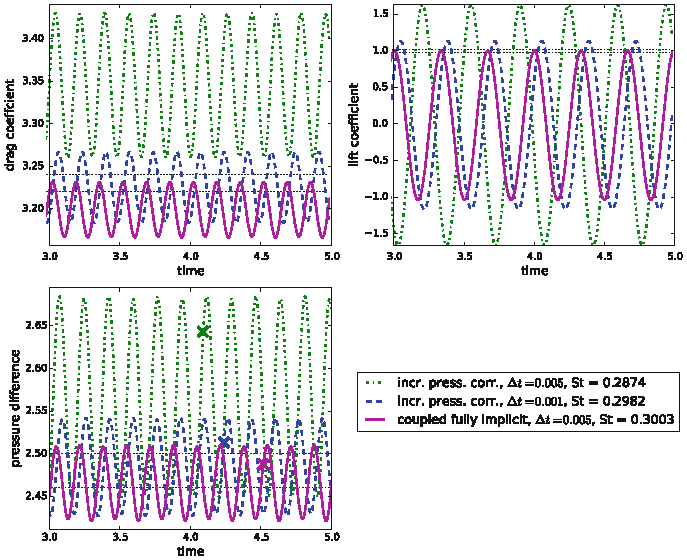
\includegraphics[width=\linewidth]{figures/Chapter_07/Fig_7_11__PDFp454__Bookp444.pdf}
\captionof{figure}{例题\hyperref[ex:incremental-pressure-correction-bdf2-cylinder]{7.101}:感兴趣量.表\hyperref[tab:appendix-d-2]{D.2}中的参考区间以点线表示;叉号标出周期的中点.Strouhal 数的参考区间为 $[0.295,0.305]$.}
\label{fig:incremental-pressure-correction-bdf2-quantities}
\end{elegantfigure}

首先,第 3 层和第 4 层网格上的结果图与图\hyperref[fig:incremental-pressure-correction-bdf2-quantities]{7.11}十分相似.因此可以看到,对全隐式方法而言,时间步长 $\Delta t=0.005$ 已足以使所有感兴趣量都落在参考区间内;而对增量压力修正格式,采用同样的时间步长会得到很不准确的结果.减小时间步长会显著提高精度;但即使取 $\Delta t=0.001$,大多数感兴趣量仍未进入各自的参考区间.总的来说,本例表明,对增量压力修正格式而言,时间离散误差占主导地位.
\end{example}
\index{压力修正格式!标准增量格式!数值结果}

\chapter{非定常 Navier--Stokes 方程组:湍流}
\label{chap:turbulent-flows}

\begin{note}[湍流]
\label{note:turbulent-flows}
通常用不可压缩 Navier--Stokes 方程组\hyperref[eq:incompressible-navier-stokes]{(2.25)}对不可压缩湍流进行建模.湍流目前没有数学上的定义.从数学角度看,湍流出现在 Reynolds 数较高时;从物理角度看,湍流的特点是流动结构的尺度大小悬殊,其中包括不同大小的涡旋(eddy).例如龙卷风,它既包含一些非常大的流动结构(大涡旋),也包含数以百万计的极小流动结构.

小尺度对湍流的物理特性十分重要.若数值格式直接忽略这些尺度,例如引入大量人工黏性,所得解就会是层流,其性质通常与湍流解大不相同.一个显著例子是槽道流动的平均速度剖面:层流时剖面呈抛物线形,而湍流时则趋于阶梯形,见图\hyperref[fig:appendix-d-12]{D.12}.对于模拟中无法分辨的小尺度,处理方法是建立模型,描述它们对已分辨尺度的影响.换言之,需要采用湍流模型(turbulence model).湍流模型所含的尺度必须少于 Navier--Stokes 方程组中的尺度,也就是说,其复杂程度必须低于 Navier--Stokes 方程组.
\end{note}


\index{湍流}
\index{湍流!涡旋}

\begin{note}[本章内容]
\label{note:turbulence-chapter-contents}
本章介绍若干湍流建模方法,重点讨论那些允许作数学或数值分析,或者其推导基于数学论证的模型,并对这些模型在实际模拟中的应用作一些说明.不过,湍流模型的实际应用是一个广阔的研究领域,本专著不打算对此作全面介绍.关于这一主题已有多部专著,例如\textcite{Sagaut2006}、\textcite{LesieurMetaisComte2005}以及\textcite{FerzigerPeric1999}.

在介绍数学和数值分析时,本章重点讨论有界区域上的结果.文献中也有许多关于空间周期情形的结果.正如笔记\hyperref[note:infinite-periodic-boundary]{2.31}中提到的,空间周期情形相当于模拟一个没有边界的区域,周期边界条件并没有物理意义.从分析角度看,没有边界可能会大幅简化分析,所采用的数学框架也与有界区域的情形有所不同.然而,在实际问题中,湍流与区域边界的相互作用往往至关重要,因此有界区域上的结果更值得关注.
\end{note}

\section{湍流不可压缩流动的若干物理与数学特征}
\label{sec:turbulence-characteristics}\label{sec:turbulence}

\begin{note}[相关专著]
\label{note:turbulence-monographs}
湍流物理是许多专著的主题,例如\textcite{Pope2000}和\textcite{Davidson2004}.\textcite{FoiasManleyRosaTemam2001}以及\textcite{ChaconRebolloLewandowski2014}研究了湍流的数学问题.
\end{note}

\begin{note}[不可压缩 Navier--Stokes 方程组]
\label{note:turbulent-navier-stokes-equations}
为描述湍流的物理特性,有时适合在黏性项中显式写出 Reynolds 数,此时不可压缩 Navier--Stokes 方程组为
\begin{equation}\label{eq:turbulent-navier-stokes}
\begin{aligned}
 \partial_t\bm{u}
 -\frac{2}{\operatorname{Re}}\nabla\cdot\mathbb{D}(\bm{u})
 +(\bm{u}\cdot\nabla)\bm{u}+\nabla p
   &=\bm{f}
      &&\text{于 }(0,T]\times\Omega,\\
 \nabla\cdot\bm{u}&=0
      &&\text{于 }(0,T]\times\Omega,\\
 \bm{u}(0,\cdot)&=\bm{u}_0
      &&\text{于 }\Omega.
\end{aligned}
\end{equation}
若 $\Omega\subset\mathbb{R}^d$($d\in\{2,3\}$)是有界区域,还须为方程\hyperref[eq:turbulent-navier-stokes]{(8.1)}配上边界条件.

湍流具有较高的 Reynolds 数.对于这类流动,应用中的 Reynolds 数通常从几千左右开始,且往往还会高出若干个数量级.Reynolds 数较高时,动量平衡中的稳定作用力——黏性项 $2\operatorname{Re}^{-1}\nabla\cdot\mathbb{D}(\bm{u})$——相对于不稳定作用力较小;后者是对流项 $\partial_t\bm{u}+(\bm{u}\cdot\nabla)\bm{u}$,即 Newton 第二运动定律\hyperref[eq:newton-second-law]{(2.5)}右端所对应的项.
\end{note}
\index{Navier--Stokes 方程组!湍流}
\index{Reynolds 数!高 Reynolds 数}

\begin{note}[瞬时流动与统计量]
\label{note:turbulent-instantaneous-flow-statistics}
讨论湍流时,人们往往认为流动在某种意义下具有混沌性,难以预测.事实上,数据发生微小变化,就可能导致瞬时流场发生很大变化;这里的瞬时流场指某一时刻 $t\in(0,T]$、某一点 $\bm{x}\in\Omega$ 处的流场.实际中,人们从来无法掌握全部数据,例如整个区域 $\Omega$ 上的初始条件,或所有时刻整个边界上的边界条件.举例来说,边界条件的测量数据只在边界上的若干点和若干时刻可得,因此方程所需的边界条件需要通过插值得到.这样获得的边界条件很可能不同于真实边界条件,因此计算所得的瞬时流场也很可能不同于真实流场.从这个角度看,研究湍流的瞬时流场并无实际意义.

实际中,人们关注的是流场的统计量,通常通过空间平均和时间平均来定义.不同问题关注的统计量也不同,例如比较例题\hyperref[ex:appendix-d-12]{D.12}和例题\hyperref[ex:appendix-d-13]{D.13}.
\end{note}
\index{湍流!瞬时流场}
\index{湍流!统计量}

\begin{note}[各向同性湍流的概念]
\label{note:isotropic-turbulence-concept}
许多湍流物理理论,例如对最小尺度大小的确定,都以各向同性湍流(isotropic turbulence)的概念为基础.若场 $\bm{u}(t,\bm{x})$ 的所有统计量在时间平移下均保持不变,则称该场为统计平稳的(statistically stationary);若所有统计量在空间平移下均保持不变,则称该场为统计均匀的(statistically homogeneous).若该场在坐标系旋转和反射下也保持统计不变,则称其为统计各向同性的(statistically isotropic),简称各向同性.

人们已经在风洞中对(近似)各向同性湍流作过实验.然而,各向同性湍流一般是一种理想化情形.
\end{note}
\index{湍流!各向同性}

\begin{note}[Richardson 能量级联]
\label{note:richardson-energy-cascade}
设 $\Omega\subset\mathbb{R}^3$.\textcite{Richardson1922}描述了湍流中的物理机制:动能从最大的涡旋输入流场;大涡旋不稳定,会破裂成更小的涡旋.由此,能量平均而言从某一尺寸的涡旋传递给下一更小尺度的涡旋.这种平均意义下的传递并不排除能量在局部(时间和空间上)沿相反方向传递,即从小涡旋传向大涡旋,主要传给紧邻的较大涡旋;这种现象称为能量回传(backscatter).小涡旋也经历与大涡旋类似的过程.该过程不断继续,直到尺度为 $\ell$ 的涡旋所对应的 Reynolds 数
\[
 \operatorname{Re}(\ell)=\frac{u(\ell)\ell}{\nu}
\]
足够小(数量级为 $1$),此时涡旋运动稳定,分子黏性开始有效耗散动能.这个过程称为能量级联(energy cascade).最小涡旋的尺度记为 $\lambda$.
\end{note}
\index{湍流!能量级联}
\index{湍流!能量回传}

\begin{note}[湍流能量耗散率]
\label{note:turbulent-energy-dissipation-rate}
以 $\varepsilon\,[\mathrm{m}^2/\mathrm{s}^3]$ 表示湍流能量耗散率(rate of dissipation of turbulent energy),其定义如下.将 $\bm{u}$ 视为随机变量,并记 $\langle\bm{u}\rangle$ 为 $\bm{u}$ 的均值(期望).差值
\[
 \bm{u}' := \bm{u}-\langle\bm{u}\rangle
\]
称为脉动量.湍流能量耗散率定义为
\[
 \varepsilon := 2\nu\langle\mathbb{D}(\bm{u}'):\mathbb{D}(\bm{u}')\rangle.
\]
对具体流动的理论和实验研究表明,
\begin{equation}\label{eq:turbulent-energy-dissipation-scaling}
 \varepsilon=\mathcal{O}\!\left(\frac{U^3}{L}\right),
\end{equation}
该关系与 Reynolds 数无关,见\textcite[p.~183]{Pope2000}.
\end{note}
\index{湍流!能量耗散率}

\begin{note}[Kolmogorov 假设]
\label{note:kolmogorov-hypotheses}
在奠基性论文\textcite{Kolmogoroff1941}中,提出了关于湍流的三个假设:
\begin{enumerate}
 \item Reynolds 数充分高时,小尺度湍流运动是各向同性的.
 \item 对于每一种 Reynolds 数充分高的湍流,小尺度运动的统计量具有普适形式,且由 $\nu$ 和 $\varepsilon$ 唯一确定.
 \item 对于每一种 Reynolds 数充分高的湍流,在尺度 $\ell$ 满足 $L\gg\ell\gg\lambda$ 的范围内,尺度为 $\ell$ 的运动统计量具有普适形式,由 $\varepsilon$ 唯一确定,且与 $\nu$ 无关.
\end{enumerate}
\end{note}
\index{湍流!Kolmogorov 假设}

\begin{note}[Kolmogorov 尺度的大小]
\label{note:kolmogorov-scale-size}
描述最小尺度大小时,Kolmogorov 假设中的第一和第二个假设尤其重要.给定 $\varepsilon$ 和 $\nu$,可定义唯一的长度、速度和时间尺度,称为 Kolmogorov 尺度:
\begin{equation}\label{eq:kolmogorov-scales}
 \lambda=\left(\frac{\nu^3}{\varepsilon}\right)^{1/4}\,[\mathrm{m}],\qquad
 u_\lambda=(\varepsilon\nu)^{1/4}\,[\mathrm{m}/\mathrm{s}],\qquad
 t_\lambda=\left(\frac{\nu}{\varepsilon}\right)^{1/2}\,[\mathrm{s}].
\end{equation}
尺度 $\lambda$ 也称为 Kolmogorov 长度尺度.尺度为 $\lambda$ 的涡旋所对应的 Reynolds 数为
\begin{equation}\label{eq:kolmogorov-reynolds-number}
 \operatorname{Re}(\lambda)=\frac{\lambda u_\lambda}{\nu}=1.
\end{equation}
因此该 Reynolds 数足够小,使黏性能够有效耗散能量.满足 $\operatorname{Re}(\lambda)=1$ 的涡旋运动是各向同性的,故符合第一个假设.

此外,利用式\hyperref[eq:kolmogorov-scales]{(8.3)},耗散率还可写为
\begin{equation}\label{eq:kolmogorov-dissipation-relations}
 \varepsilon^{1/2}=\frac{u_\lambda^2}{\nu^{1/2}},\qquad
 \varepsilon^{1/2}=\frac{\nu^{3/2}}{\lambda^2}
 \quad\Longrightarrow\quad
 \varepsilon=\frac{\nu u_\lambda^2}{\lambda^2}
 \quad\text{且}\quad
 \varepsilon=\frac{\nu}{t_\lambda^2}.
\end{equation}
于是
\begin{equation}\label{eq:kolmogorov-velocity-gradient}
 \frac{u_\lambda}{\lambda}
  =\frac{1}{t_\lambda}
  =\left(\frac{\varepsilon}{\nu}\right)^{1/2}
  \quad[1/\mathrm{s}].
\end{equation}
左端近似于 Kolmogorov 速度的空间导数,它描述速度梯度;这是因为 $\lambda$ 很小.对湍流中的大涡旋,流场在时空中的变化很快,因此速度梯度会随 Reynolds 数增加.式\hyperref[eq:kolmogorov-velocity-gradient]{(8.6)}表明,对于 Kolmogorov 尺度,速度梯度关于 Reynolds 数一致有界;它只依赖于 $\nu$ 和 $\varepsilon$.第二个 Kolmogorov 假设正是要求这种依赖形式.总之,式\hyperref[eq:kolmogorov-reynolds-number]{(8.4)}和式\hyperref[eq:kolmogorov-velocity-gradient]{(8.6)}将 Kolmogorov 尺度刻画为耗散尺度.

现在可以估计 Kolmogorov 尺度的大小.利用式\hyperref[eq:turbulent-energy-dissipation-scaling]{(8.2)}和式\hyperref[eq:kolmogorov-scales]{(8.3)},得到
\begin{equation}\label{eq:kolmogorov-length-reynolds-scaling}
 \frac{\lambda}{L}
 \sim\left(\frac{\nu^3}{L^3U^3}\right)^{1/4}
 \sim\operatorname{Re}^{-3/4}
 \quad\Longleftrightarrow\quad
 \lambda\sim\operatorname{Re}^{-3/4},
\end{equation}
其中假设 $L\sim1\,\mathrm{m}$.
\end{note}
\index{Kolmogorov 尺度}
\index{湍流!耗散尺度}

\begin{note}[Kolmogorov 尺度大小对数值模拟的影响]
\label{note:kolmogorov-scales-numerical-impact}
Navier--Stokes 方程组\hyperref[eq:turbulent-navier-stokes]{(8.1)}的一种标准离散方法,例如第\hyperref[sec:time-dependent-fem-continuous]{7.2 节}研究的 Galerkin 有限元方法,旨在模拟所有尺度的行为,包括 Kolmogorov 尺度.

例如,考虑区域 $\Omega=(0,1)^3$,于是 $L=1$;并设网格约有 $10^8$ 个立方网格单元(约为 $464^3$ 个).若假设网格宽度等于离散分辨率,这对低阶有限元是合理的,则此网格可以表示大小为 $1/464$ 的尺度.只有能够在网格上表示出来的尺度才可以模拟.因此,要在该网格上模拟某种流动,其 Kolmogorov 长度至少须满足 $\lambda\gtrsim1/464$.进一步假设式\hyperref[eq:turbulent-energy-dissipation-scaling]{(8.2)}取等号,则由式\hyperref[eq:kolmogorov-length-reynolds-scaling]{(8.7)}可知,可模拟的流动 Reynolds 数最高约为 $\operatorname{Re}\approx464^{4/3}\approx3590$.这一数值远低于大多数应用中湍流的 Reynolds 数.

对一般情形作同样的估算,由式\hyperref[eq:kolmogorov-length-reynolds-scaling]{(8.7)}可知,解析 Kolmogorov 尺度所需的自由度数满足
\[
 \left(\frac{L}{\lambda}\right)^3\sim\operatorname{Re}^{9/4}.
\]
在湍流模拟中,采用 Galerkin 有限元方法(或任何其他标准离散方法)称为直接数值模拟(direct numerical simulation,DNS).本注记中的估算表明,一般而言,DNS 不适用于湍流模拟;在可预见的未来,这种情况也不会改变.
\end{note}
\index{直接数值模拟(DNS)}
\index{Kolmogorov 尺度!数值分辨率}

\begin{note}[动能谱]
\label{note:turbulent-kinetic-energy-spectrum}
能量级联(笔记\hyperref[note:richardson-energy-cascade]{8.7})和 Kolmogorov 的第三个假设(笔记\hyperref[note:kolmogorov-hypotheses]{8.9})可用动能谱(kinetic energy spectrum)来表达.

设 $\Omega=\mathbb{R}^3$,速度场为 $\bm{u}(t,\bm{x})$.对其应用 Fourier 变换(Fourier transform)\hyperref[eq:appendix-a-23]{(A.23)},得到
\[
 \mathcal{F}(\bm{u})(t,\bm{k})
  =\int_{\mathbb{R}^3}
    \bm{u}(t,\bm{x})e^{-i\bm{k}\cdot\bm{x}}\,\mathrm{d}\bm{x}.
\]
其中 $\bm{k}=(k_1,k_2,k_3)^\mathsf{T}$ 为波数向量;Fourier 空间称为波数空间(wave number space).波数 $\bm{k}$ 对应的动能定义为
\[
 E(t,\bm{k})
  =\frac12\left\langle
    \mathcal{F}(\bm{u})(t,\bm{k})\cdot
    \mathcal{F}(\bm{u})^*(t,\bm{k})
   \right\rangle,
\]
其中 $\mathcal{F}(\bm{u})^*$ 表示 $\mathcal{F}(\bm{u})$ 的复共轭,$\langle\cdot\rangle$ 表示适当的均值.这里考虑平均速度为零的均匀各向同性湍流.对绝对值相同的波数 $k=\|\bm{k}\|_2$,定义
\[
 E(t,k)=\int_{\|\bm{k}\|_2=k}E(t,\bm{k})\,\mathrm{d}\bm{k}.
\]
Kolmogorov 的第三个假设意味着,对于满足 $L\gg\ell\gg\lambda$ 的尺度 $\ell$,其统计量具有普适形式.图\hyperref[fig:turbulent-kinetic-energy-spectrum]{8.1}示意了湍流的动能谱;详细推导见\textcite[p.~229]{Pope2000}.在所谓的惯性子区(inertial subrange)内,有
\[
 E(k)=C_K\varepsilon^{2/3}k^{-5/3}.
\]
其中 $C_K$ 称为 Kolmogorov 常数.这一关系通常称为 Kolmogorov $-5/3$ 谱.高 Reynolds 数流动具有明显的惯性子区,而层流中没有这一子区.

\begin{elegantfigure}[0.82\linewidth]

\includegraphics[page=461,pagebox=cropbox,trim=53.00bp 99.40bp 53.11bp 331.50bp,clip,width=\linewidth]{../input/source/Finite Element Methods for Incompressible Flow Problems.pdf}
\captionof{figure}{湍流动能谱示意图.}
\label{fig:turbulent-kinetic-energy-spectrum}
\end{elegantfigure}
\end{note}
\index{湍流!动能谱}
\index{Kolmogorov 谱}

\begin{note}[边界层]
\label{note:turbulent-boundary-layers}
以湍流槽道流动为例,见例题\hyperref[ex:appendix-d-12]{D.12}.边界是一块位于 $y=0$ 的平面固壁,区域在其 $y>0$ 一侧,并在该壁面施加无滑移条件 $\bm{u}=0$.此时,边界附近形成一层流体.对于平均速度场,有 $\langle u_1\rangle=\langle u_1\rangle(y)$,且 $\langle u_2\rangle=\langle u_3\rangle=0$.于是,平均速度对应的黏性应力\hyperref[eq:viscous-stress-law]{(2.17)}为
\[
 \rho\nu\frac{\nabla\langle\bm{u}\rangle
             +(\nabla\langle\bm{u}\rangle)^\mathsf{T}}{2}
 =\frac{\rho\nu}{2}
 \begin{pmatrix}
  0&\partial_y\langle u_1\rangle&0\\
  \partial_y\langle u_1\rangle&0&0\\
  0&0&0
 \end{pmatrix}.
\]
壁面上的平均黏性应力,即所谓壁面剪切应力(wall shear stress),其唯一非零分量为
\[
 \tau_w=\left.\rho\nu\,\partial_y\langle u_1\rangle\right|_{y=0}
 \quad[\mathrm{N}/\mathrm{m}^2].
\]
这里单位的写法假定速度具有量纲.利用 $\tau_w$,可以为近壁区域定义合适的速度尺度和长度尺度,从而在不依赖 Reynolds 数的情况下刻画该边界层.速度尺度称为摩擦速度(friction velocity),定义为
\[
 U_\tau=\sqrt{\frac{\tau_w}{\rho}}
 \quad[\mathrm{m}/\mathrm{s}],
\]
黏性长度尺度(viscous length scale)为
\[
 \lambda_\nu=\nu\sqrt{\frac{\rho}{\tau_w}}
  =\frac{\nu}{U_\tau}
 \quad[\mathrm{m}].
\]
于是,无量纲壁面距离可用黏性长度或壁面单位(wall units)表示为
\[
 y^+=\frac{y}{\lambda_\nu}=\frac{U_\tau}{\nu}y.
\]
根据 $y^+$ 的大小,可以区分若干近壁流动区域.$y^+<50$ 的区域称为黏性壁面区(viscous wall region),此处的分子黏性效应不可忽略.$y^+<5$ 时,黏性应力 $\tau_w$ 甚至支配该区域的流动行为,因此这一区域称为黏性底层(viscous sublayer).$y^+>50$ 的区域称为外层(outer layer).
\end{note}
\index{湍流!边界层}
\index{壁面剪切应力}
\index{摩擦速度}
\index{黏性长度尺度}

\begin{note}[二维流动与三维流动的差异]
\label{note:two-three-dimensional-flow-differences}
二维流动与三维流动至少存在两个根本差异.

首先,二维流动中的最小尺度不同于式\hyperref[eq:kolmogorov-length-reynolds-scaling]{(8.7)}所给的规律.\textcite{Kraichnan1967}证明,二维流动的最小尺度为 $\lambda_{2d}\sim\operatorname{Re}^{-1/2}$;其中 $\lambda_{2d}$ 称为 Kraichnan 耗散长度(Kraichnan dissipation length).

第二个差异是所谓的涡拉伸(vortex stretching).涡量(vorticity)定义为 $\symbfit{\Omega}=\nabla\times\bm{u}$,见定义\hyperref[def:rotation-curl]{3.162}.对 Navier--Stokes 方程组\hyperref[eq:turbulent-navier-stokes]{(8.1)}施加旋度算子,并假设函数足够光滑.对于黏性项,利用式\hyperref[eq:viscous-term-laplacian]{(2.27)}、Schwarz 定理,再次利用式\hyperref[eq:viscous-term-laplacian]{(2.27)},以及由式\hyperref[eq:divergence-curl-zero]{(3.157)}得到的 $\nabla\cdot\symbfit{\Omega}=0$,可得
\[
\begin{aligned}
 2\nabla\times\bigl(\nabla\cdot\mathbb{D}(\bm{u})\bigr)
 &=\nabla\times(\Delta\bm{u})\\
 &=\begin{pmatrix}
   \partial_y\Delta u_3-\partial_z\Delta u_2\\
   \partial_z\Delta u_1-\partial_x\Delta u_3\\
   \partial_x\Delta u_2-\partial_y\Delta u_1
  \end{pmatrix}\\
 &=\Delta\begin{pmatrix}
   \partial_yu_3-\partial_zu_2\\
   \partial_zu_1-\partial_xu_3\\
   \partial_xu_2-\partial_yu_1
  \end{pmatrix}
 =\Delta(\nabla\times\bm{u})\\
 &=\Delta\symbfit{\Omega}
  =2\nabla\cdot\mathbb{D}(\symbfit{\Omega}).
\end{aligned}
\]
对于对流项,利用式\hyperref[eq:steady-ns-rotational-identity]{(6.6)}、式\hyperref[eq:curl-gradient-zero]{(3.156)}和式\hyperref[eq:curl-cross-product-divergence]{(3.159)},并再次使用 $\nabla\cdot\symbfit{\Omega}=0$,可得
\[
\begin{aligned}
 \nabla\times\bigl((\bm{u}\cdot\nabla)\bm{u}\bigr)
 &=\nabla\times\left(
      (\nabla\times\bm{u})\times\bm{u}
      +\frac12\nabla(\bm{u}^{\mathsf{T}}\bm{u})
    \right)\\
 &=\nabla\times(\symbfit{\Omega}\times\bm{u})\\
 &=(\bm{u}\cdot\nabla)\symbfit{\Omega}
   -(\symbfit{\Omega}\cdot\nabla)\bm{u}.
\end{aligned}
\]
因此,当 $\bm{f}=0$ 时,Navier--Stokes 方程组对应的涡量方程为
\[
 \partial_t\symbfit{\Omega}
 -2\operatorname{Re}^{-1}\nabla\cdot\mathbb{D}(\symbfit{\Omega})
 +(\bm{u}\cdot\nabla)\symbfit{\Omega}
 -(\symbfit{\Omega}\cdot\nabla)\bm{u}=0.
\]
当 Reynolds 数较高时,黏性项较小,可以忽略.因此
\begin{equation}\label{eq:vorticity-transport-vortex-stretching}
 \frac{D\symbfit{\Omega}}{Dt}
  =\frac{\partial\symbfit{\Omega}}{\partial t}
    +(\bm{u}\cdot\nabla)\symbfit{\Omega}
  \approx(\symbfit{\Omega}\cdot\nabla)\bm{u}.
\end{equation}
这就是物质微小线元的演化方程.如果 $\nabla\bm{u}$ 使线元伸长,$|\symbfit{\Omega}|$ 也会随之增大.事实上,三维湍流中会发生涡拉伸,这是这类流动的重要特征.涡拉伸会改变局部长度尺度,并产生一系列不同大小的涡结构.因此,涡拉伸是湍流具有多尺度特征的原因之一.

在二维流动中,式\hyperref[eq:vorticity-transport-vortex-stretching]{(8.8)}右端为零,因此不会发生涡拉伸.由于没有涡拉伸,且黏性长度尺度的大小也不同,高 Reynolds 数下的二维流动在性质上与三维湍流不同.因此,可以认为二维流动中不存在湍流.不过,在二维问题上检验新的高 Reynolds 数流动方法仍然是合理的:如果方法在二维下失效,那么它在还具有额外复杂特征的三维流动中成功的可能性不大;反过来,若方法在二维下成功,也不能不经数值研究便断定它在三维中同样有效.
\end{note}
\index{湍流!涡量}
\index{湍流!涡拉伸}
\index{Kraichnan 耗散长度}

\begin{note}[研究湍流的数学方法]
\label{note:dynamical-systems-turbulence}
研究湍流的一种数学概念是在动力系统理论中发展起来的.动力系统的形式为
\begin{equation}\label{eq:dynamical-system-abstract}
 \frac{\mathrm{d}\bm{u}}{\mathrm{d}t}
  =F(\bm{u}),
 \qquad \bm{u}_0=\bm{u}(0).
\end{equation}
在弱无散空间\hyperref[eq:time-dependent-ns-weak-first]{(7.3)}中,不可压缩 Navier--Stokes 方程组符合这一框架,其中
\[
 F(\bm{u})=\bm{f}-\nu A\bm{u}-N(\bm{u},\bm{u}),
\]
这里 $A:V_{\mathrm{div}}\to V'$ 是以分布意义定义的 Laplace 算子,满足
\[
 (\nabla\bm{u},\nabla\bm{v})
  =\langle A\bm{u},\bm{v}\rangle_{V',V}
  \qquad\forall\bm{v}\in V_{\mathrm{div}},
\]
而 $N:V_{\mathrm{div}}\times V_{\mathrm{div}}\to V'$ 是双线性对流算子,满足
\[
 (N(\bm{u},\bm{v}),\bm{w})
  =n(\bm{u},\bm{v},\bm{w})
  \qquad\forall\bm{u},\bm{v},\bm{w}\in V_{\mathrm{div}}.
\]
Navier--Stokes 方程组的理论通常假定体力与时间无关,即 $\bm{f}(t,\bm{x})=\bm{f}(\bm{x})$.此时得到自治动力系统(autonomous dynamical system).

为了研究动力系统的解集,可以定义吸引子(attractor),见笔记\hyperref[note:global-attractor]{8.18},特别是吸引子的维数.\textcite[p.~380]{Temam1997}写道:“我们在此将湍流现象的自由度数理解为代表该现象的吸引子的维数.”

下面将简要介绍这一概念,并概述不可压缩 Navier--Stokes 方程组的一些结果.更详细的介绍可见\textcite[第 III 章]{FoiasManleyRosaTemam2001}或\textcite[第 13 章]{MarionTemam1998}.
\end{note}
\index{动力系统}
\index{自治动力系统}
\index{吸引子}

\begin{note}[描述动力系统演化的一族算子]
\label{note:dynamical-system-semigroup}\label{note:semigroup-method}
考虑自治动力系统\hyperref[eq:dynamical-system-abstract]{(8.9)},并假设它存在唯一解.定义算子族 $\{S(t)\}_{t\ge0}$:
\[
 S(t):\bm{u}(0)\mapsto\bm{u}(t)
 \quad\Longleftrightarrow\quad
 \bm{u}(t)=S(t)\bm{u}(0).
\]
也就是说,该算子将初始条件映射为时刻 $t$ 的解.它具有以下基本性质:
\begin{itemize}
 \item $S(0)=I$,其中 $I$ 是恒等算子.
 \item 对任意 $s,t\ge0$,时刻 $t+s$ 的解相同,无论是从时刻 $0$ 出发直接演化至 $t+s$,还是先从 $0$ 演化至 $t$,再继续演化至 $t+s$.数学上,这一性质写为
  \[
  \begin{aligned}
   \bm{u}(t+s)&=S(t+s)\bm{u}(0)\\
    &=S(s)\bigl(S(t)\bm{u}(0)\bigr)\\
    &=\bigl(S(s)\circ S(t)\bigr)\bm{u}(0),
      \qquad\forall s,t\ge0.
  \end{aligned}
  \]
 或者
 \[
  S(t+s)=S(s)\circ S(t)=S(t)\circ S(s)
   \qquad\forall s,t\ge0.
 \]
\end{itemize}
因此,算子族 $\{S(t)\}_{t\ge0}$ 构成半群(semigroup),但不存在逆元.
\end{note}
\index{半群}

\begin{note}[不可压缩 Navier--Stokes 方程组的框架]
\label{note:navier-stokes-dynamical-system-setup}
对不可压缩 Navier--Stokes 方程组,假设 $\bm{u}_0,\bm{f}\in H_{\mathrm{div}}(\Omega)$.目前只在二维情形下知道该方程组存在唯一解,见定理\hyperref[thm:time-dependent-two-dimensional-uniqueness]{7.24}.此时可以证明 $S(t)$ 是 $H_{\mathrm{div}}(\Omega)$ 上的连续算子,见\textcite[p.~554]{MarionTemam1998}以及\textcite[p.~138]{FoiasManleyRosaTemam2001}.
\end{note}

\begin{note}[全局吸引子]
\label{note:global-attractor}
半群 $\{S(t)\}_{t\ge0}$ 的全局吸引子(global attractor)是集合 $\mathcal{A}\subset H_{\mathrm{div}}(\Omega)$,具有下列性质:
\begin{itemize}
 \item 集合 $\mathcal{A}$ 在 $H_{\mathrm{div}}(\Omega)$ 中是紧的.
 \item 集合 $\mathcal{A}$ 对半群是不变的,即对所有 $t\ge0$,有 $S(t)\mathcal{A}=\mathcal{A}$.
 \item 集合 $\mathcal{A}$ 吸引 $H_{\mathrm{div}}(\Omega)$ 中的所有有界集:对每个有界集 $B\subset H_{\mathrm{div}}(\Omega)$,有
 \[
  \operatorname{dist}_{H_{\mathrm{div}}(\Omega)}(S(t)B,\mathcal{A})
   =\sup_{\bm{b}\in S(t)B}\inf_{\bm{a}\in\mathcal{A}}
      \|\bm{a}-\bm{b}\|_{L^2(\Omega)}
   \longrightarrow0
   \qquad\text{当 }t\to\infty.
 \]
 也就是说,两个集合之间的距离随 $t\to\infty$ 趋于零.
\end{itemize}
若全局吸引子存在,则可以证明它是唯一的.
\end{note}
\index{全局吸引子}

\begin{note}[全局吸引子的 Hausdorff 维数]
\label{note:global-attractor-hausdorff-dimension}
不可压缩 Navier--Stokes 方程组的全局吸引子的 Hausdorff 维数(Hausdorff dimension)尤其重要,见\textcite[p.~117]{FoiasManleyRosaTemam2001}.给定集合 $X$ 和 $\varepsilon>0$,用半径不超过 $\varepsilon$ 的 $\hat d$ 维球覆盖 $X$,其中 $\hat d\in\mathbb{R}$.这些球的体积与 $\varepsilon^{\hat d}$ 成正比.定义
\[
 \mu_H(X,\hat d,\varepsilon)
  =\inf_{\{B_i\}_{i\in I}}\sum_{i\in I}r_i^{\hat d},
\]
其中下确界取遍 $X$ 的所有覆盖:每个覆盖均由球族 $\{B_i\}_{i\in I}$ 组成,且球 $B_i$ 的半径为 $r_i\le\varepsilon$.减小最大半径时,覆盖体积不会增加,因此 $\mu_H(X,\hat d,\varepsilon)$ 关于 $\varepsilon$ 单调不增.于是
\[
 \mu_H(X,\hat d)
  =\lim_{\varepsilon\to0}\mu_H(X,\hat d,\varepsilon)
\]
是集合 $X$ 的 $\hat d$ 维 Hausdorff 测度.可以证明,存在 $d_0\in[0,\infty]$,使得当 $\hat d<d_0$ 时 $\mu_H(X,\hat d)=\infty$,当 $\hat d>d_0$ 时 $\mu_H(X,\hat d)=0$.数 $d_0$ 称为 $X$ 的 Hausdorff 维数,记为 $d_H(X)$.
\end{note}
\index{Hausdorff 维数}

\begin{note}[二维 Navier--Stokes 方程组的结果]
\label{note:two-dimensional-navier-stokes-results}
由于二维不可压缩 Navier--Stokes 方程组存在唯一解,可以定义半群 $\{S(t)\}_{t\ge0}$ 并研究其性质.\textcite{FoiasTemam1979}在 $\Omega$ 边界光滑的情形下证明了全局吸引子的存在性及其 Hausdorff 维数有限.此后有多种推广,特别是对周期情形的推广;综述见\textcite[p.~140]{FoiasManleyRosaTemam2001}.\textcite{Temam1986}给出了 Hausdorff 维数的一个估计.可以证明
\[
 d_H(\mathcal{A})\lesssim
  \left(\frac{L}{\lambda_{2d}}\right)^2,
\]
见\textcite[p.~141]{FoiasManleyRosaTemam2001};其中 $\lambda_{2d}$ 在笔记\hyperref[note:two-three-dimensional-flow-differences]{8.14}中引入.
\end{note}

\begin{note}[三维 Navier--Stokes 方程组的推广]
\label{note:three-dimensional-navier-stokes-extensions}
对三维 Navier--Stokes 方程组,可以考虑 $V_{\mathrm{div}}$ 中的有界不变集,见\textcite[p.~147]{FoiasManleyRosaTemam2001}.若集合 $X\subset V_{\mathrm{div}}$ 中任一初值 $\bm{u}_0\in X$ 所对应的唯一局部解(见笔记\hyperref[note:time-dependent-local-existence-small-data]{7.26})都能延拓为唯一的全局解 $\bm{u}(t)$,使得其对所有 $t\ge0$ 均有定义且取值于 $X$,则称 $X$ 为不变集.\textcite{ConstantinFoiasManleyTemam1985b}和\textcite{ConstantinFoiasTemam1985a}证明,任意有界不变集 $X\subset V_{\mathrm{div}}$ 的 Hausdorff 维数,其自由度数量级与 Kolmogorov 理论的预测一致,参见笔记\hyperref[note:kolmogorov-scales-numerical-impact]{8.11},即
\begin{equation}\label{eq:hausdorff-dimension-three-dimensional-invariant-set}
 d_H(X)\sim\left(\frac{L}{\lambda}\right)^3.
\end{equation}
\end{note}
\index{Navier--Stokes 方程组!二维}
\index{Navier--Stokes 方程组!三维}
\index{不变集}

\begin{note}[湍流模型的复杂度较低]
\label{note:smaller-complexity-turbulence-models}
如笔记\hyperref[note:turbulent-flows]{8.1}所述,湍流模型的复杂程度必须低于不可压缩 Navier--Stokes 方程组.每一种湍流模型都含有一个参数,用来确定需要模拟的尺度.该参数通常与(局部)网格宽度有关,例如 Smagorinsky 大涡模拟(LES)模型中的参数(见式\hyperref[eq:smagorinsky-filter-width]{(8.67)}),因为网格宽度决定了哪些尺度能够表示出来.因此,实际计算中,网格越细,该参数越小;当网格宽度趋于零时,湍流模型渐近地收敛到 Navier--Stokes 方程组.

为了研究湍流模型的复杂度是否较低,可以像第\hyperref[sec:smagorinsky-analysis]{8.3.2 节}那样固定该参数,并考察湍流模型的连续对应问题.复杂度降低的一个标志是存在长时间弱解及其唯一性;Navier--Stokes 方程组的解的唯一性目前尚未得到证明,见笔记\hyperref[note:time-dependent-three-dimensional-uniqueness]{7.25}.另一个标志是其全局吸引子的维数小于式\hyperref[eq:hausdorff-dimension-three-dimensional-invariant-set]{(8.10)}所示的数量级.

有限元误差分析还提供了另一个标志:可以证明误差估计不依赖 Reynolds 数,而依赖某种降低后的 Reynolds 数.例如,三尺度粗空间投影型变分多尺度方法的定理\hyperref[thm:three-level-projection-vms-velocity-error]{8.273}即属此类.
\end{note}

\section{大涡模拟:空间平均的概念}
\label{sec:large-eddy-space-averaging}

\subsection{LES 基本概念、空间平均与滤波函数卷积}
\label{subsec:les-basic-concept-space-averaging}

\begin{note}[大涡模拟的基本思想]
\label{note:large-eddy-simulation-basic-idea}
对于湍流,在某种意义上,给定网格通常只能表示较大的尺度,也只有这些尺度能够被模拟;这一问题见笔记\hyperref[note:kolmogorov-scales-numerical-impact]{8.11}.确定哪些尺度属于大尺度有多种方法.大涡模拟(Large Eddy Simulation,LES)通过空间平均来定义大尺度;理论上,空间平均通常由滤波函数与流场的卷积给出.

采用这种方法,可以将 Navier--Stokes 方程组的解分解为
\begin{equation}\label{eq:les-scale-decomposition}
 \bm{u}=\overline{\bm{u}}+\bm{u}',
 \qquad
 p=\overline{p}+p'.
\end{equation}
式\hyperref[eq:les-scale-decomposition]{(8.11)}中,$(\overline{\bm{u}},\overline{p})$ 表示大尺度部分;$(\bm{u}',p')$ 表示小尺度部分,也称未解析尺度、亚格子尺度或脉动量.
\end{note}
\index{大涡模拟(LES)}
\index{大尺度}
\index{未解析尺度}
\index{亚格子尺度}

\begin{note}[卷积形式的空间平均、滤波函数与波数]
\label{note:space-averaging-convolution-filter-wave-number}
设 $v(t,\bm{x})$ 是定义在 $\mathbb{R}^d$ 上的充分光滑函数.给定适当的滤波函数 $g_{\mathrm{fil}}(\bm{x})$,通过卷积定义其空间平均:
\begin{equation}\label{eq:space-average-convolution}
\begin{aligned}
 \overline{v}(t,\bm{x})
  &=(g_{\mathrm{fil}}*v)(t,\bm{x})\\
  &=\int_{\mathbb{R}^d}
      g_{\mathrm{fil}}(\bm{x}-\bm{z})v(t,\bm{z})
      \,\mathrm{d}\bm{z}\\
  &=\int_{\mathbb{R}^d}
      g_{\mathrm{fil}}(\bm{z})v(t,\bm{x}-\bm{z})
      \,\mathrm{d}\bm{z}.
\end{aligned}
\end{equation}
最后一个等号来自积分变量的变换.为简明起见,考虑一维情形.先令 $w=x-z$,再交换积分上下限,可得
\[
 \int_{-\infty}^{\infty}g_{\mathrm{fil}}(x-z)v(z)\,\mathrm{d}z
 =-\int_{\infty}^{-\infty}g_{\mathrm{fil}}(w)v(x-w)\,\mathrm{d}w
 =\int_{-\infty}^{\infty}g_{\mathrm{fil}}(z)v(x-z)\,\mathrm{d}z.
\]
对式\hyperref[eq:space-average-convolution]{(8.12)}作 Fourier 变换,并利用式\hyperref[eq:appendix-a-25]{(A.25)},得到
\begin{equation}\label{eq:fourier-transform-space-average}
 \mathcal{F}(\overline{v})(t,\bm{k})
  =\bigl(\mathcal{F}(g_{\mathrm{fil}})
         \mathcal{F}(v)\bigr)(t,\bm{k}).
\end{equation}
其中 $\bm{k}$ 是对偶变量,也称波数.若当 $\|\bm{k}\|_2>k_c$ 时
$\mathcal{F}(g_{\mathrm{fil}})(t,\bm{k})=0$,其中 $k_c$ 为截断波数,则将 $v$ 与 $g_{\mathrm{fil}}$ 卷积会滤除 $v(t,\bm{x})$ 的所有高波数分量.高波数分量对应于 $v$ 的脉动.这是理想情形;实际应用中,只要充分快速地衰减高波数就足够了.因此,滤波函数的一个重要要求是其 Fourier 变换在高波数处快速衰减.

假设滤波函数 $g_{\mathrm{fil}}(\bm{x})$ 可以表示为一维滤波函数的张量积:
\begin{equation}\label{eq:filter-tensor-product}
 g_{\mathrm{fil}}(\bm{x})
  =\prod_{i=1}^{d}g_{\mathrm{fil},i}(x_i).
\end{equation}
由于各因子所依赖的变量不同,滤波函数的 Fourier 变换为
\[
 \mathcal{F}(g_{\mathrm{fil}})(\bm{k})
  =\prod_{i=1}^{d}\mathcal{F}(g_{\mathrm{fil},i})(k_i).
\]

定义 $\overline{v}$ 时的滤波作用,通常用一个正数 $\delta$ 来描述.$\delta$ 称为特征滤波宽度、平均半径或滤波尺度.滤波宽度衡量被衰减涡旋的大小;被衰减的涡旋尺度均小于 $\mathcal{O}(\delta)$.显然,$\delta$ 越小,截断波数 $k_c$ 越大,被滤除的涡旋就越少.
\end{note}
\index{空间平均}
\index{卷积}
\index{滤波函数}
\index{截断波数}
\index{波数}
\index{特征滤波宽度}

\begin{example}[高斯滤波器]
\label{ex:gaussian-filter}
高斯滤波器是大涡模拟中最常用的滤波器之一.其滤波函数为
\begin{equation}\label{eq:gaussian-filter-one-dimensional}
 g_{\mathrm{fil},i}(x_i)
  =g_{\mathrm{Gauss},i}(x_i)
  =\sqrt{\frac{6}{\pi\delta^2}}\,
    \exp\!\left(-\frac{6}{\delta^2}x_i^2\right).
\end{equation}
利用
\[
 \int_0^\infty e^{-ax^2}\,\mathrm{d}x
   =\frac12\sqrt{\frac{\pi}{a}},
 \qquad a>0,
\]
以及对称性,可得
\begin{equation}\label{eq:gaussian-integral}
 \int_{-\infty}^{\infty}e^{-ax^2}\,\mathrm{d}x
   =\sqrt{\frac{\pi}{a}},
 \qquad a>0.
\end{equation}
于是,由 Fourier 变换的定义(式\hyperref[eq:appendix-a-23]{(A.23)})有
\begin{equation}\label{eq:gaussian-filter-fourier-one-dimensional}
\begin{aligned}
 \mathcal{F}(g_{\mathrm{Gauss},j})(k_j)
  &=\sqrt{\frac{6}{\pi\delta^2}}
    \int_{-\infty}^{\infty}
      \exp\!\left(-\frac{6}{\delta^2}x_j^2-ik_jx_j\right)
      \,\mathrm{d}x_j\\
  &=\sqrt{\frac{6}{\pi\delta^2}}\,
    \exp\!\left(-\frac{k_j^2\delta^2}{24}\right)
    \int_{-\infty}^{\infty}
      \exp\!\left[-\left(
       \frac{\sqrt{6}}{\delta}x_j+
       \frac{ik_j\delta}{2\sqrt{6}}\right)^2\right]
      \,\mathrm{d}x_j\\
  &=\sqrt{\frac{6}{\pi\delta^2}}\,
    \frac{\delta}{\sqrt{6}}\,
    \exp\!\left(-\frac{k_j^2\delta^2}{24}\right)
    \int_{-\infty}^{\infty}e^{-y^2}\,\mathrm{d}y\\
  &=\exp\!\left(-\frac{k_j^2\delta^2}{24}\right),
  \qquad j=1,\ldots,d.
\end{aligned}
\end{equation}
式\hyperref[eq:gaussian-filter-one-dimensional]{(8.15)}中的系数经过选择,使高斯滤波器的滤波作用与某个模型问题中的离散近似的滤波作用相匹配;详细讨论见\textcite[Sect.~3.8]{Aldama1990}.此外,滤波函数的积分已归一化,见式\hyperref[eq:gaussian-filter-integrability]{(8.21)}.高斯滤波函数与其 Fourier 变换具有相同形式.

在 $\mathbb{R}^d$ 上,高斯滤波器为
\begin{equation}\label{eq:gaussian-filter-d-dimensional}
 g_{\mathrm{Gauss}}(\bm{x})
  =\left(\frac{6}{\delta^2\pi}\right)^{d/2}
    \exp\!\left(-\frac{6}{\delta^2}\|\bm{x}\|_2^2\right).
\end{equation}
\begin{elegantfigure}[0.72\linewidth]
 
\includegraphics[page=470,pagebox=cropbox,trim=162.50bp 423.40bp 51.61bp 60.50bp,clip,width=\linewidth]{../input/source/Finite Element Methods for Incompressible Flow Problems.pdf}
 \captionof{figure}{不同滤波宽度 $\delta$ 下的一维高斯滤波函数.}
 \label{fig:gaussian-filter}
\end{elegantfigure}
见图\hyperref[fig:gaussian-filter]{8.2}.其 Fourier 变换为
\begin{equation}\label{eq:gaussian-filter-fourier}
 \mathcal{F}(g_{\mathrm{Gauss}})(\bm{k})
  =\exp\!\left(-\frac{\delta^2}{24}\|\bm{k}\|_2^2\right).
\end{equation}

为简化记号,下文中高斯滤波器以标量 $x$ 为自变量时,约定
\[
 g_{\mathrm{Gauss}}(x)
  :=\left(\frac{6}{\delta^2\pi}\right)^{d/2}
    \exp\!\left(-\frac{6x^2}{\delta^2}\right).
\]
高斯滤波器具有下列性质.这些性质可由指数函数的性质直接推出,也可通过直接计算验证;亦可参见图\hyperref[fig:gaussian-filter]{8.2}.
\begin{itemize}
 \item \textit{正则性:}由于指数函数无穷次可微,
 \[
  g_{\mathrm{Gauss}}\in C^\infty(\mathbb{R}^d),
  \qquad
  \mathcal{F}(g_{\mathrm{Gauss}})\in C^\infty(\mathbb{R}^d).
 \]
 \item \textit{正性:}指数函数为正,且式\hyperref[eq:gaussian-filter-d-dimensional]{(8.18)}和式\hyperref[eq:gaussian-filter-fourier]{(8.19)}在原点取最大值,故
 \begin{equation}\label{eq:gaussian-filter-positivity}
  0<g_{\mathrm{Gauss}}(\bm{x})
    \le\left(\frac{6}{\delta^2\pi}\right)^{d/2},
  \qquad
  0<\mathcal{F}(g_{\mathrm{Gauss}})(\bm{k})\le1.
 \end{equation}
 \item \textit{可积性:}由式\hyperref[eq:gaussian-integral]{(8.16)}可得
 \[
  \|g_{\mathrm{Gauss}}\|_{L^p(\mathbb{R}^d)}
   =\left(\frac{6}{\delta^2\pi}\right)^{d/2}
    \left(\frac{\delta^2\pi}{6p}\right)^{d/(2p)}.
 \]
 因而
 \begin{equation}\label{eq:gaussian-filter-integrability}
  \|g_{\mathrm{Gauss}}\|_{L^p(\mathbb{R}^d)}<\infty
   \quad\forall p\in[1,\infty],
  \qquad
  \|g_{\mathrm{Gauss}}\|_{L^1(\mathbb{R}^d)}=1.
 \end{equation}
 \item \textit{对称性:}式\hyperref[eq:gaussian-filter-d-dimensional]{(8.18)}和式\hyperref[eq:gaussian-filter-fourier]{(8.19)}只依赖于 $\bm{x}$ 和 $\bm{k}$ 的 Euclidean 范数,因此
 \begin{equation}\label{eq:gaussian-filter-symmetry}
  g_{\mathrm{Gauss}}(\bm{x})=g_{\mathrm{Gauss}}(-\bm{x}),
  \qquad
  \mathcal{F}(g_{\mathrm{Gauss}})(\bm{k})
   =\mathcal{F}(g_{\mathrm{Gauss}})(-\bm{k}).
 \end{equation}
 \item \textit{单调性:}由指数函数的单调性可知,若 $\|\bm{x}\|_2\le\|\bm{y}\|_2$,则
 \begin{equation}\label{eq:gaussian-filter-monotonicity}
  g_{\mathrm{Gauss}}(\bm{x})\ge g_{\mathrm{Gauss}}(\bm{y}).
 \end{equation}
\end{itemize}
\end{example}
\index{高斯滤波器}
\index{Fourier 变换}

\begin{lemma}[高斯滤波器的其他性质]
\label{lem:gaussian-filter-properties}
\begin{enumerate}[label=\roman*)]
 \item 设 $\varphi\in L^p(\mathbb{R}^d)$,其中 $1\le p<\infty$.则
 \begin{equation}\label{eq:gaussian-filter-approximate-identity}
  \lim_{\delta\to0}
   \|g_{\mathrm{Gauss}}*\varphi-\varphi\|_{L^p(\mathbb{R}^d)}=0.
 \end{equation}
 \item 设 $\varphi\in L^\infty(\mathbb{R}^d)$,且 $\varphi$ 在集合 $\Omega$ 上一致连续,则当 $\delta\to0$ 时,$g_{\mathrm{Gauss}}*\varphi$ 在 $\Omega$ 上一致收敛到 $\varphi$.
\end{enumerate}
\end{lemma}
\begin{proof}
前两条结论的证明可见例如 \textcite[Theorem~0.13]{Folland1995}.
\end{proof}



\begin{example}[方框滤波器]
\label{ex:box-filter}
另一种常用滤波器是方框滤波器(box filter),也称顶帽滤波器(top hat filter).在一维情形,给定滤波宽度 $\delta>0$,定义
\[
 g_{\mathrm{box}}(x)=
 \begin{cases}
  \dfrac{1}{\delta},&x\in[-\delta/2,\delta/2],\\[4pt]
  0,&\text{其他情形}.
 \end{cases}
\]
见图\hyperref[fig:box-filter]{8.3}.多维方框滤波器由式\hyperref[eq:filter-tensor-product]{(8.14)}所示的张量积定义.方框滤波器的主要性质如下:
\begin{elegantfigure}[0.84\linewidth]
 
\includegraphics[page=472,pagebox=cropbox,trim=52.50bp 467.65bp 53.36bp 60.75bp,clip,width=\linewidth]{../input/source/Finite Element Methods for Incompressible Flow Problems.pdf}
 \captionof{figure}{不同滤波宽度 $\delta$ 下的一维方框滤波函数(左)及其 Fourier 变换(右).}
 \label{fig:box-filter}
\end{elegantfigure}
\begin{itemize}
 \item 它是分段常数函数;
 \item 它非负;
 \item 它具有紧支集:
 \[
  \operatorname{supp}(g_{\mathrm{box}})
   =[-\delta/2,\delta/2];
 \]
 \item 对 $p\in[1,\infty]$,有 $g_{\mathrm{box}}\in L^p(\mathbb{R})$,且
 \[
  \|g_{\mathrm{box}}\|_{L^1(\mathbb{R})}=1;
 \]
 \item 对 Fourier 变换(式\hyperref[eq:appendix-a-23]{(A.23)}),利用微积分基本定理和复指数的 Euler 公式,可得
 \[
 \begin{aligned}
  \mathcal{F}(g_{\mathrm{box},j})(k_j)
   &=\int_{-\delta/2}^{\delta/2}
      \frac{1}{\delta}e^{-ik_jx_j}\,\mathrm{d}x_j\\
   &=\frac{1}{\delta}\left(-\frac{1}{ik_j}\right)
      \left(
       e^{-ik_j\delta/2}-e^{ik_j\delta/2}
      \right)\\
   &=\frac{2}{k_j\delta}
      \sin\!\left(\frac{k_j\delta}{2}\right).
 \end{aligned}
 \]
 当 $k_j=0$ 时,上式按连续延拓取值 $1$.
\end{itemize}
因此,方框滤波器的 Fourier 变换是一个衰减的正弦函数.该函数会取负值,见图\hyperref[fig:box-filter]{8.3}.
\end{example}
\index{方框滤波器}
\index{顶帽滤波器}
\index{高斯滤波器!逼近恒等算子}

\subsection{全空间上的空间平均 Navier--Stokes 方程组}
\label{subsec:les-space-averaged-equations-full-space}

\begin{note}[推导大涡模拟模型的步骤]
\label{note:steps-deriving-les-models}
为了计算空间平均速度 $\overline{\bm{u}}$ 和压力 $\overline{p}$,需要推导描述这两个量的方程;这些方程须从 $\bm{u}$ 和 $p$ 所满足的控制方程,即 Navier--Stokes 方程组推导而来.第一步是将用于定义 $(\overline{\bm{u}},\overline{p})$ 的滤波算子施加于 Navier--Stokes 方程组\hyperref[eq:incompressible-navier-stokes]{(2.25)}.因此,大涡模拟建模以 Navier--Stokes 方程组的强形式为基础;这与其他一些湍流模型不同,后者以 Navier--Stokes 方程组的变分形式为基础,例如见第\hyperref[sec:variational-multiscale-methods]{8.8 节}.将滤波算子施加于方程组\hyperref[eq:incompressible-navier-stokes]{(2.25)}后,若假设卷积与微分可交换,就得到 LES 的基本方程,即空间平均 Navier--Stokes 方程组.然而,由于 Navier--Stokes 方程组含有非线性项,还需要额外的建模步骤,才能从空间平均 Navier--Stokes 方程组中得到关于 $(\overline{\bm{u}},\overline{p})$ 的封闭方程.

第\hyperref[sec:large-eddy-space-averaging]{8.2 节}余下部分将研究卷积与微分可交换这一假设.额外的建模步骤将在第\hyperref[sec:les-models]{8.3 节}和第\hyperref[sec:les-wave-number-models]{8.4 节}讨论.
\end{note}

\begin{note}[滤波算子的假设]
\label{note:assumptions-filter-operator}
假设定义 $(\overline{\bm{u}},\overline{p})$ 的滤波算子具有下列性质.
\begin{itemize}
 \item 滤波算子是线性的:
 \begin{equation}\label{eq:filter-linearity}
  \overline{u+\lambda v}=\overline{u}+\lambda\overline{v}.
 \end{equation}
 \item 微分运算(空间一阶和二阶导数、时间一阶导数)可与滤波平均交换.例如,
 \begin{equation}\label{eq:filter-commutation-space-derivative}
  \overline{\partial_{x_i}u}
   =\partial_{x_i}\overline{u},
  \qquad i=1,\ldots,d,
 \end{equation}
 且
 \begin{equation}\label{eq:filter-commutation-time-derivative}
  \overline{\partial_t u}=\partial_t\overline{u}.
 \end{equation}
\end{itemize}
经典微积分已经表明,对含参数函数求导与积分可交换,需要该函数关于参数具有充分的光滑性.
\end{note}

\begin{note}[全空间情形下的卷积滤波]
\label{note:convolution-filtering-full-space}
令 $\Omega=\mathbb{R}^d$,并取式\hyperref[eq:space-average-convolution]{(8.12)}所定义的滤波函数卷积作为滤波算子.注意,该滤波算子只在 $\mathbb{R}^d$ 上有定义.积分算子的线性性直接推出式\hyperref[eq:filter-linearity]{(8.25)}.关于时间导数的交换性质\hyperref[eq:filter-commutation-time-derivative]{(8.27)},则来自对一个变量积分与对另一个变量求导可以交换这一事实.

为得到性质\hyperref[eq:filter-commutation-space-derivative]{(8.26)},还需假设滤波宽度 $\delta$ 为常数.设函数充分光滑.先利用卷积表示\hyperref[eq:space-average-convolution]{(8.12)}作积分变量变换 $\bm{w}=\bm{x}-\bm{z}$,再用 Fubini 定理交换积分次序、变回原积分变量,并应用链式法则.对 $i=1,\ldots,d$,有
\[
 \partial_{x_i}v
  =\sum_{j=1}^d\partial_{z_j}v\,\partial_{x_i}z_j
  =\sum_{j=1}^d\partial_{z_j}v\,\delta_{ij}
  =\partial_{z_i}v.
\]
因此,
\[
\begin{aligned}
 \partial_{x_i}\overline{v}(t,\bm{x})
  &=\partial_{x_i}
    \int_{\mathbb{R}^d}
     g_{\mathrm{fil}}(\bm{w})
     v(t,\bm{x}-\bm{w})\,\mathrm{d}\bm{w}\\
  &=\int_{\mathbb{R}^d}
     g_{\mathrm{fil}}(\bm{w})
     \partial_{x_i}v(t,\bm{x}-\bm{w})\,\mathrm{d}\bm{w}\\
  &=\int_{\mathbb{R}^d}
     g_{\mathrm{fil}}(\bm{x}-\bm{z})
     \partial_{z_i}v(t,\bm{z})\,\mathrm{d}\bm{z}\\
  &=\overline{\partial_{x_i}v}(t,\bm{x}).
\end{aligned}
\]
\end{note}

\begin{note}[全空间上的空间平均 Navier--Stokes 方程组]
\label{note:space-averaged-ns-full-space}
将具有性质\hyperref[eq:filter-linearity]{(8.25)}和\hyperref[eq:filter-commutation-space-derivative]{(8.26)}的滤波算子施加于 Navier--Stokes 方程组\hyperref[eq:incompressible-navier-stokes]{(2.25)},并假设函数和初值 $\bm{u}_0$ 充分光滑,便得到空间平均 Navier--Stokes 方程组(也称 Reynolds 方程组):
\begin{equation}\label{eq:space-averaged-navier-stokes-full-space}
\begin{aligned}
 \partial_t\overline{\bm{u}}
  -2\nu\nabla\cdot\mathbb{D}(\overline{\bm{u}})
  +\nabla\cdot\overline{\bm{u}\bm{u}^{\mathsf T}}
  +\nabla\overline{p}
   &=\overline{\bm{f}}
      &&\text{于 }(0,T]\times\mathbb{R}^d,\\
 \nabla\cdot\overline{\bm{u}}
   &=0
      &&\text{于 }(0,T]\times\mathbb{R}^d,\\
 \overline{\bm{u}}(0,\cdot)
   &=\overline{\bm{u}}_0
      &&\text{于 }\mathbb{R}^d.
\end{aligned}
\end{equation}
\end{note}
\index{Reynolds 方程组}

\begin{note}[非线性项的滤波与封闭问题]
\label{note:les-closure-problem}
空间平均 Navier--Stokes 方程组\hyperref[eq:space-averaged-navier-stokes-full-space]{(8.28)}还不是关于 $(\overline{\bm{u}},\overline{p})$ 的封闭方程,因为张量 $\overline{\bm{u}\bm{u}^{\mathsf T}}$ 尚未用 $(\overline{\bm{u}},\overline{p})$ 表示.$d$ 维向量与自身的张量积是对称张量,因此 $\overline{\bm{u}\bm{u}^{\mathsf T}}$ 也是对称的.一方面,式\hyperref[eq:space-averaged-navier-stokes-full-space]{(8.28)}有 $d+1$ 个方程;另一方面,除 $d+1$ 个空间平均未知量外,张量 $\overline{\bm{u}\bm{u}^{\mathsf T}}$ 还包含 $d(d+1)/2$ 个未知量.因此出现了封闭问题.将非线性项写成
\begin{equation}\label{eq:subgrid-stress-decomposition}
\begin{aligned}
 \nabla\cdot\overline{\bm{u}\bm{u}^{\mathsf T}}
  &=\nabla\cdot
       \bigl(\overline{\bm{u}}\,
             \overline{\bm{u}}^{\mathsf T}\bigr)
    +\nabla\cdot
       \bigl(\overline{\bm{u}\bm{u}^{\mathsf T}}
             -\overline{\bm{u}}\,
              \overline{\bm{u}}^{\mathsf T}\bigr)\\
  &=\nabla\cdot
       \bigl(\overline{\bm{u}}\,
             \overline{\bm{u}}^{\mathsf T}\bigr)
    +\nabla\cdot\mathbb{T},
\end{aligned}
\end{equation}
其中 $\mathbb{T}$ 称为亚格子尺度(sgs)应力张量(subgrid-scale stress tensor;见\textcite{MeneveauKatz2000})、亚格子张量(subgrid tensor;见\textcite[p.~49]{Sagaut2006})、残余应力张量(residual-stress tensor;见\textcite[p.~581]{Pope2000}),也称 Reynolds 应力张量.为了封闭方程,必须建立亚格子尺度张量的模型.用 $(\overline{\bm{u}},\overline{p})$ 表示 $\mathbb{T}$,是 LES 的核心问题.第\hyperref[sec:les-models]{8.3 节}和第\hyperref[sec:les-wave-number-models]{8.4 节}将讨论这一主题.
\end{note}
\index{封闭问题}
\index{亚格子尺度应力张量}
\index{残余应力张量}
\index{Reynolds 应力张量}

\begin{note}[时间平均]
\label{note:time-averaging-not-les}
大涡模拟的概念不包含时间平均.时间平均用于推导 Reynolds 平均 Navier--Stokes(RANS)模型;更多细节见例如\textcite[Sect.~9.4]{FerzigerPeric1999}.
\end{note}
\index{时间平均}
\index{Reynolds 平均 Navier--Stokes(RANS)模型}

\subsection{有界区域上的空间平均 Navier--Stokes 方程组}
\label{subsec:les-space-averaged-equations-bounded-domain}

\begin{note}[实际计算中有界区域上的空间平均 Navier--Stokes 方程组]
\label{note:les-bounded-domain-practical-computations}
实际计算中,通常也会在有界区域 $\Omega$ 上使用式\hyperref[eq:space-averaged-navier-stokes-full-space]{(8.28)},也就是将其中的 $\mathbb{R}^d$ 换成 $\Omega$,并在滤波算子\hyperref[eq:space-average-convolution]{(8.12)}的定义中作同样替换.然而,从数学角度看,若 $\Omega$ 是有界区域,滤波与微分的可交换性就需要特别处理.必须将 Navier--Stokes 方程组中的所有函数一致地从 $\Omega$ 延拓到 $\mathbb{R}^d$.一般而言,这些延拓不够光滑,因此微分与积分不能简单地交换;此时会出现一个额外项.省略该项便会产生所谓的交换误差(commutation error).下文将研究这类交换误差.

本部分的论述依据\textcite{DuncaJohnLayton2004}.
\end{note}
\index{交换误差}

\begin{note}[问题的设置]
\label{note:les-bounded-domain-problem-setup}
设 $\Omega\subset\mathbb{R}^d$ 是有界区域,$d\in\{2,3\}$,边界 $\partial\Omega$ 为 Lipschitz 边界,且其 $(d-1)$ 维测度满足 $|\partial\Omega|<\infty$.考虑具有齐次 Dirichlet 边界条件的不可压缩 Navier--Stokes 方程组:
\begin{equation}\label{eq:les-bounded-domain-ns}
\begin{aligned}
 \partial_t\bm{u}
  -2\nu\nabla\cdot\mathbb{D}(\bm{u})
  +\nabla\cdot(\bm{u}\bm{u}^{\mathsf T})
  +\nabla p
   &=\bm{f}
      &&\text{于 }(0,T]\times\Omega,\\
 \nabla\cdot\bm{u}
   &=0
      &&\text{于 }(0,T]\times\Omega,\\
 \bm{u}
   &=0
      &&\text{于 }(0,T]\times\partial\Omega,\\
 \bm{u}(0,\cdot)
   &=\bm{u}_0
      &&\text{于 }\Omega,\\
 \int_\Omega p\,\mathrm{d}\bm{x}
   &=0
      &&\text{于 }(0,T].
\end{aligned}
\end{equation}

推导空间平均 Navier--Stokes 方程组并分析交换误差,需要方程组\hyperref[eq:les-bounded-domain-ns]{(8.30)}存在唯一解 $(\bm{u},p)$,且解充分正则,使法向应力在 $\partial\Omega$ 上具有良好定义的迹,并属于边界上某个 Lebesgue 空间.应力张量 $\bm{S}$ 见式\hyperref[eq:dimensionless-stress-tensor]{(2.35)};边界 $\partial\Omega$ 上的法向应力,也称 Cauchy 应力向量,为 $\bm{S}\bm{n}$.具体假设如下:
\begin{equation}\label{eq:les-bounded-domain-regularity}
\begin{aligned}
 \bm{u}&\in H^2(\Omega)\cap V,\qquad
 p\in H^1(\Omega)\cap Q
 &&\text{对几乎处处的 }t\in[0,T],\\
 \bm{u}&\in H^1(0,T)
 &&\text{对几乎处处的 }\bm{x}\in\Omega.
\end{aligned}
\end{equation}

为了将卷积算子施加于方程组\hyperref[eq:les-bounded-domain-ns]{(8.30)},必须先将所有函数延拓到区域之外.这些延拓函数将在分布意义下满足 Navier--Stokes 方程组.于是可以施加卷积算子;在 $\mathbb{R}^d$ 上滤波与微分可交换,从而得到空间平均 Navier--Stokes 方程组.
\end{note}

\begin{lemma}[法向应力的正则性及其 $L^p(\partial\Omega)$ 估计]
\label{lem:les-normal-stress-regularity}
若假设\hyperref[eq:les-bounded-domain-regularity]{(8.31)}成立,则
$\bm{S}\bm{n}\in H^{1/2}(\partial\Omega)$.特别地,对几乎处处的
$t\in[0,T]$,有
\[
 \bm{S}\bm{n}\in L^q(\partial\Omega),
 \qquad
 \begin{cases}
  q\in[1,\infty),&d=2,\\
  q\in[1,4],&d=3.
 \end{cases}
\]
\end{lemma}
\begin{proof}
由迹定理、定理\hyperref[thm:appendix-a-34]{A.34}及式\hyperref[eq:appendix-a-11]{(A.11)}(取 $s=1$),可知 $\nabla\bm{u}\in H^{1/2}(\partial\Omega)$ 且 $p\in H^{1/2}(\partial\Omega)$,从而 $\bm{S}\bm{n}\in H^{1/2}(\partial\Omega)$.定理\hyperref[thm:appendix-a-34]{A.34}在 $q=2$ 时还给出了引理的第二个结论.
\end{proof}

\begin{note}[将函数延拓到 $\mathbb{R}^d$]
\label{note:les-function-extensions}
为了推导可以施加滤波函数卷积的方程,必须先将 $\bm{f}$ 延拓到 $\Omega$ 之外,再使 $(\bm{u},p)$ 与 $\bm{f}$ 的延拓相容地延拓,从而令延拓后的函数满足某种 Navier--Stokes 方程组.由于右端是给定数据,必须预先知道 $\bm{f}$ 的延拓.为了便于计算,将 $\bm{f}$ 在 $\Omega$ 外延拓为零.于是也可将 $(\bm{u},p)$ 在 $\Omega$ 外延拓为零.由于 $\bm{u}=0$ 于 $\partial\Omega$,这种延拓是合理的.因此,定义
\[
 \bm{u}=0,\qquad
 \bm{u}_0=0,\qquad
 p=0,\qquad
 \bm{f}=0
 \quad\text{若 }\bm{x}\notin\Omega.
\]
延拓后的函数具有以下正则性:
\begin{equation}\label{eq:les-zero-extension-regularity}
\begin{aligned}
 \bm{u}&\in H_0^1(\mathbb{R}^d),\qquad
 p\in L_0^2(\mathbb{R}^d)
 &&\text{对几乎处处的 }t\in[0,T],\\
 \bm{u}&\in H^1(0,T)
 &&\text{对几乎处处的 }\bm{x}\in\mathbb{R}^d.
\end{aligned}
\end{equation}
由式\hyperref[eq:les-bounded-domain-regularity]{(8.31)}和式\hyperref[eq:les-zero-extension-regularity]{(8.32)}可知,延拓速度场的一阶弱导数 $\partial_t\bm{u}$、$\nabla\bm{u}$、$\nabla\cdot\bm{u}$ 以及 $\nabla\cdot(\bm{u}\bm{u}^{\mathsf T})$ 在 $\mathbb{R}^d$ 上均有良好定义;它们在 $\Omega$ 上取原有的值,在 $\Omega$ 外恒为零.

确实存在一个将 $\bm{u}$ 从 $\Omega$ 延拓到 $\mathbb{R}^d$ 上且属于 $H^2(\mathbb{R}^d)$ 的延拓,但该延拓未知;特别是因为我们并不知道边界以外的 $\bm{u}$.若采用这种延拓,而不采用在 $\mathbb{R}^d\setminus\Omega$ 上令 $\bm{u}=0$ 的方式,就会导致 $\bm{f}$ 的延拓未知,从而空间平均动量方程中的 $\bm{f}$ 也无法确定.
\end{note}
\index{零延拓}
\index{法向应力}
\index{Cauchy 应力向量}

\begin{note}[压力项与黏性项的延拓]
\label{note:extension-pressure-viscous-terms}
由于 $\bm{u}\notin H^2(\mathbb{R}^d)$、$p\notin H^1(\mathbb{R}^d)$,必须在分布意义下定义 $\nabla\cdot\mathbb{D}(\bm{u})$ 和 $\nabla p$.为此,取 $\varphi\in C_0^\infty(\mathbb{R}^d)$.由于对所有时刻,$p$ 在 $\mathbb{R}^d\setminus\Omega$ 上恒为零,按照分布导数的定义并作分部积分,对 $i=1,\ldots,d$ 有
\[
\begin{aligned}
 (\partial_i p)(\varphi)(t)
  &=-\int_{\mathbb{R}^d}
        p(t,\bm{x})\partial_i\varphi(\bm{x})
        \,\mathrm{d}\bm{x}\\
  &=\int_\Omega
       \varphi(\bm{x})\partial_i p(t,\bm{x})
       \,\mathrm{d}\bm{x}
    -\int_{\partial\Omega}
       p(t,\bm{s})\varphi(\bm{s})
       \bm{e}_i\cdot\bm{n}(\bm{s})\,\mathrm{d}s,
\end{aligned}
\]
或者用紧凑形式写为
\begin{equation}\label{eq:distributional-pressure-gradient}
\begin{aligned}
 (\nabla p)(\varphi)(t)
  &=-\int_{\mathbb{R}^d}
      p(t,\bm{x})\nabla\varphi(\bm{x})
      \,\mathrm{d}\bm{x}\\
  &=\int_\Omega
       \varphi(\bm{x})\nabla p(t,\bm{x})
       \,\mathrm{d}\bm{x}
    -\int_{\partial\Omega}
       p(t,\bm{s})\varphi(\bm{s})
       \bm{n}(\bm{s})\,\mathrm{d}s.
\end{aligned}
\end{equation}
同理可得
\begin{equation}\label{eq:distributional-viscous-divergence}
\begin{aligned}
 (\nabla\cdot\mathbb{D}(\bm{u}))(\varphi)(t)
  &=-\int_{\mathbb{R}^d}
       \mathbb{D}(\bm{u})(t,\bm{x})
       \nabla\varphi(\bm{x})\,\mathrm{d}\bm{x}\\
  &=\int_\Omega
       \varphi(\bm{x})\nabla\cdot\mathbb{D}(\bm{u})(t,\bm{x})
       \,\mathrm{d}\bm{x}
    -\int_{\partial\Omega}
       \varphi(\bm{s})\mathbb{D}(\bm{u})(t,\bm{s})
       \bm{n}(\bm{s})\,\mathrm{d}s.
\end{aligned}
\end{equation}
这两个分布都定义了 $C_0^\infty(\mathbb{R}^d)$ 上的连续线性泛函,且具有紧支集.注意,由正则性假设\hyperref[eq:les-bounded-domain-regularity]{(8.31)}可知,$p$ 和 $\mathbb{D}(\bm{u})$ 在 $\partial\Omega$ 上的迹均有良好定义.
\end{note}

\begin{note}[动量方程的分布形式]
\label{note:distributional-momentum-equation}
由式\hyperref[eq:distributional-pressure-gradient]{(8.33)}和式\hyperref[eq:distributional-viscous-divergence]{(8.34)}可知,延拓函数 $(\bm{u},p)$ 满足以下动量方程的分布形式:
\begin{equation}\label{eq:distributional-momentum-equation}
\begin{aligned}
 &\bigl(
   \partial_t\bm{u}
   -2\nu\nabla\cdot\mathbb{D}(\bm{u})
   +\nabla\cdot(\bm{u}\bm{u}^{\mathsf T})
   +\nabla p
  \bigr)(\varphi)(t)\\
 &\qquad
  =\int_\Omega
      \bm{f}(t,\bm{x})\varphi(\bm{x})
      \,\mathrm{d}\bm{x}
    +\int_{\partial\Omega}
      \bm{S}(t,\bm{s})\bm{n}(\bm{s})
      \varphi(\bm{s})\,\mathrm{d}s,
 \qquad
 \forall\varphi\in C_0^\infty(\mathbb{R}^d).
\end{aligned}
\end{equation}
\end{note}

\begin{note}[有界区域上的空间平均 Navier--Stokes 方程组]
\label{note:space-averaged-ns-bounded-domain}
现在通过将滤波函数 $g_{\mathrm{fil}}(\bm{x})\in C^\infty(\mathbb{R}^d)$ 与式\hyperref[eq:distributional-momentum-equation]{(8.35)}卷积,来推导空间平均 Navier--Stokes 方程组.将 $g_{\mathrm{fil}}$ 与式\hyperref[eq:distributional-momentum-equation]{(8.35)}卷积后,得到一个 $C^\infty(\mathbb{R}^d)$ 函数;并且在 $\mathbb{R}^d$ 上卷积与微分可交换,见\textcite[Theorem~4.1.1]{Hormander1990}.因此,式\hyperref[eq:distributional-momentum-equation]{(8.35)}左端满足
\begin{equation}\label{eq:filtered-distributional-momentum-left}
\begin{aligned}
 &g_{\mathrm{fil}}*
  \bigl[
   (\partial_t\bm{u}
    -2\nu\nabla\cdot\mathbb{D}(\bm{u})
    +\nabla\cdot(\bm{u}\bm{u}^{\mathsf T})
    +\nabla p)(\varphi)
  \bigr]\\
 &=\partial_t\overline{\bm{u}}
   -2\nu\nabla\cdot\mathbb{D}(\overline{\bm{u}})
   +\nabla\cdot\overline{\bm{u}\bm{u}^{\mathsf T}}
   +\nabla\overline{p},
\end{aligned}
\end{equation}
其中 $(t,\bm{x})\in(0,T]\times\mathbb{R}^d$.

接下来详细考察黏性项和压力项的滤波.设 $H(\varphi)$ 是一个具有紧支集的分布,且可写成
\[
 H(\varphi)
  =-\int_{\mathbb{R}^d}
      f(\bm{x})D^\alpha\varphi(\bm{x})
      \,\mathrm{d}\bm{x},
\]
其中 $D^\alpha$ 表示由多重指标 $\alpha$ 给出的 $\varphi$ 的导数.由\textcite[Theorem~6.35]{Rudin1991}可知,
$H*g_{\mathrm{fil}}\in C^\infty(\mathbb{R}^d)$,并且
\begin{equation}\label{eq:distribution-convolution-representation}
\begin{aligned}
 H(\bm{x})
  &=(H*g_{\mathrm{fil}})(\bm{x})\\
  &=H\bigl(g_{\mathrm{fil}}(\bm{x}-\cdot)\bigr)\\
  &=-\int_{\mathbb{R}^d}
      f(\bm{y})D^\alpha
        g_{\mathrm{fil}}(\bm{x}-\bm{y})
      \,\mathrm{d}\bm{y}.
\end{aligned}
\end{equation}
将式\hyperref[eq:distribution-convolution-representation]{(8.37)}用于式\hyperref[eq:distributional-pressure-gradient]{(8.33)},得到
\begin{equation}\label{eq:filtered-pressure-gradient-bounded-domain}
\begin{aligned}
 \nabla\overline{p}(t,\bm{x})
  &=g_{\mathrm{fil}}*
       \bigl((\nabla p)(\varphi)\bigr)(t,\bm{x})\\
  &=-\int_{\mathbb{R}^d}
       p(t,\bm{y})\nabla
       g_{\mathrm{fil}}(\bm{x}-\bm{y})
       \,\mathrm{d}\bm{y}\\
  &=\int_\Omega
       \nabla p(t,\bm{y})g_{\mathrm{fil}}(\bm{x}-\bm{y})
       \,\mathrm{d}\bm{y}
    -\int_{\partial\Omega}
       g_{\mathrm{fil}}(\bm{x}-\bm{s})p(t,\bm{s})
       \bm{n}(\bm{s})\,\mathrm{d}s.
\end{aligned}
\end{equation}
以相同方式将式\hyperref[eq:distributional-viscous-divergence]{(8.34)}卷积,可得
\begin{equation}\label{eq:filtered-viscous-divergence-bounded-domain}
\begin{aligned}
 \nabla\cdot\mathbb{D}(\overline{\bm{u}})(t,\bm{x})
  &=\int_\Omega
       \nabla\cdot\mathbb{D}(\bm{u})(t,\bm{y})
       g_{\mathrm{fil}}(\bm{x}-\bm{y})\,\mathrm{d}\bm{y}\\
  &\quad
    -\int_{\partial\Omega}
       g_{\mathrm{fil}}(\bm{x}-\bm{s})
       \mathbb{D}(\bm{u})(t,\bm{s})
       \bm{n}(\bm{s})\,\mathrm{d}s.
\end{aligned}
\end{equation}
结合式\hyperref[eq:filtered-distributional-momentum-left]{(8.36)}、\hyperref[eq:filtered-pressure-gradient-bounded-domain]{(8.38)}和\hyperref[eq:filtered-viscous-divergence-bounded-domain]{(8.39)},得到空间平均动量方程
\begin{equation}\label{eq:space-averaged-momentum-bounded-domain}
\begin{aligned}
 \partial_t\overline{\bm{u}}
  -2\nu\nabla\cdot\mathbb{D}(\overline{\bm{u}})
  +\nabla\cdot\overline{\bm{u}\bm{u}^{\mathsf T}}
  +\nabla\overline{p}
  &=\overline{\bm{f}}
    +\int_{\partial\Omega}
       g_{\mathrm{fil}}(\bm{x}-\bm{s})
       \bm{S}(t,\bm{s})\bm{n}(\bm{s})\,\mathrm{d}s\\
  &\qquad\text{于 }(0,T]\times\mathbb{R}^d,
\end{aligned}
\end{equation}
其中
\begin{equation}\label{eq:filtered-body-force-bounded-domain}
\begin{aligned}
 \overline{\bm{f}}(t,\bm{x})
  =\int_\Omega
     \bigl(
       \partial_t\bm{u}
       -2\nu\nabla\cdot\mathbb{D}(\bm{u})
       +\nabla\cdot(\bm{u}\bm{u}^{\mathsf T})
       +\nabla p
     \bigr)(t,\bm{y})
     g_{\mathrm{fil}}(\bm{x}-\bm{y})\,\mathrm{d}\bm{y}.
\end{aligned}
\end{equation}
由于 $\bm{f}$ 在 $t\in(0,T]$ 时于 $\Omega$ 外为零,式\hyperref[eq:filtered-body-force-bounded-domain]{(8.41)}与直接滤波 $\bm{f}$ 所得的形式相同.对函数作一致延拓后,理应得到这种对应关系.
\end{note}

\begin{definition}[交换误差]
\label{def:les-commutation-error}
设 $g_{\mathrm{fil}}\in C^\infty(\mathbb{R}^d)$ 为滤波宽度为 $\delta$ 的滤波函数.空间平均 Navier--Stokes 方程组中的交换误差 $\mathcal{A}_\delta(\bm{S})$ 定义为
\[
 \mathcal{A}_\delta(\bm{S})(t,\bm{x})
  =\int_{\partial\Omega}
     g_{\mathrm{fil}}(\bm{x}-\bm{s})
     \bm{S}(t,\bm{s})\bm{n}(\bm{s})\,\mathrm{d}s.
\]
\end{definition}
\index{交换误差}

\begin{note}[关于交换误差]
\label{note:remarks-on-commutation-error}
\begin{itemize}
 \item 交换误差的分析将针对例题\hyperref[ex:gaussian-filter]{8.25}中定义的高斯滤波器 $g_{\mathrm{Gauss}}$ 进行.
 \item 分析交换误差时,固定任意一个 $t\in(0,T]$,从而可以忽略 $\mathcal{A}_\delta(\bm{S})$ 对时间的依赖.
 \item 若 Navier--Stokes 方程组中的黏性项写为 $\nu\Delta\bm{u}$,而不是 $2\nu\nabla\cdot\mathbb{D}(\bm{u})$,则在式\hyperref[eq:space-averaged-momentum-bounded-domain]{(8.40)}中用 $\nabla\overline{\bm{u}}$ 代替 $2\mathbb{D}(\overline{\bm{u}})$,并在应力张量中用 $\nabla\bm{u}(t,\bm{s})$ 代替 $2\mathbb{D}(\bm{u})(t,\bm{s})$,即可得到相应的空间平均动量方程.
 \item 因此,由有界区域上的 Navier--Stokes 方程组得到的空间平均方程含有额外的边界积分 $\mathcal{A}_\delta(\bm{S})$.省略该积分就会产生交换误差.若将该积分纳入空间平均动量方程,则会引出新的建模问题:它依赖于 $(\bm{u},p)$ 在 $\partial\Omega$ 上的未知法向应力,而不依赖于 $(\overline{\bm{u}},\overline{p})$.
\end{itemize}
\end{note}
\index{交换误差!法向应力项}

\subsection{高斯滤波器的交换误差分析}
\label{subsec:gaussian-filter-commutation-error}

\begin{note}[待研究的项]
\label{note:commutation-term-studied}
根据定义\hyperref[def:les-commutation-error]{8.41}、引理\hyperref[lem:les-normal-stress-regularity]{8.36}和笔记\hyperref[note:remarks-on-commutation-error]{8.42},需要研究下列形式的项:
\begin{equation}\label{eq:commutation-error-integral}
 \int_{\partial\Omega}
   g_{\mathrm{Gauss}}(\bm{x}-\bm{s})\psi(\bm{s})\,\mathrm{d}s.
\end{equation}
其中 $\psi\in L^q(\partial\Omega)$,$1\le q\le\infty$.回忆一下,假设 $\partial\Omega$ 具有有限的 $(d-1)$ 维测度.
\end{note}

\begin{lemma}[式\hyperref[eq:commutation-error-integral]{(8.42)}定义了 $L^p(\mathbb{R}^d)$ 函数]
\label{lem:gaussian-commutation-Lp}
设 $\psi\in L^q(\partial\Omega)$,$1\le q\le\infty$.则式\hyperref[eq:commutation-error-integral]{(8.42)}属于 $L^p(\mathbb{R}^d)$,对任意 $1\le p\le\infty$ 均成立.
\end{lemma}
\begin{proof}
分情形证明.
\begin{enumerate}[label=\roman*)]
 \item $p=\infty$ 且 $q>1$.由 Hölder 不等式(见式\hyperref[eq:appendix-a-9]{(A.9)}),取 $r^{-1}+q^{-1}=1$,有
 \begin{equation}\label{eq:commutation-error-Lp-pointwise}
 \begin{aligned}
  \left|\int_{\partial\Omega}
    g_{\mathrm{Gauss}}(\bm{x}-\bm{s})\psi(\bm{s})\,\mathrm{d}s\right|
  &\!\le\!
    \|g_{\mathrm{Gauss}}(\bm{x}-\cdot)\|_{L^r(\partial\Omega)}\\
  &\quad\cdot\|\psi\|_{L^q(\partial\Omega)}\\
  &=\left(\frac{6}{\delta^2\pi}\right)^{d/2}\\
  &\times
    \left(\int_{\partial\Omega}
      \exp\!\left(-\frac{6r}{\delta^2}
                  \|\bm{x}-\bm{s}\|_2^2\right)\,\mathrm{d}s\right)^{1/r}\\
  &\quad\times\|\psi\|_{L^q(\partial\Omega)}.
 \end{aligned}
 \end{equation}
 由三角不等式和 Young 不等式(见式\hyperref[eq:appendix-a-5]{(A.5)}),
 \[
  \|\bm{x}\|_2^2
   \le 2\|\bm{x}-\bm{s}\|_2^2+2\|\bm{s}\|_2^2
  \quad\Longleftrightarrow\quad
  2\|\bm{x}-\bm{s}\|_2^2
   \ge \|\bm{x}\|_2^2-2\|\bm{s}\|_2^2.
 \]
 因此,利用指数函数的单调性可得
 \[
  \exp\!\left(-\frac{6r}{\delta^2}
                  \|\bm{x}-\bm{s}\|_2^2\right)
  \le
  \exp\!\left(\frac{3r}{\delta^2}
        \bigl(-\|\bm{x}\|_2^2+2\|\bm{s}\|_2^2\bigr)\right).
 \]
 将此估计代入式\hyperref[eq:commutation-error-Lp-pointwise]{(8.43)},得到
 \begin{equation}\label{eq:commutation-error-Linfty-bound}
 \begin{aligned}
  \left|\int_{\partial\Omega}
    g_{\mathrm{Gauss}}(\bm{x}-\bm{s})\psi(\bm{s})\,\mathrm{d}s\right|
  &\le
   \left(\frac{6}{\delta^2\pi}\right)^{d/2}
   \|\psi\|_{L^q(\partial\Omega)}\\
  &\quad\times\left(\int_{\partial\Omega}
      \exp\!\left(\frac{6r}{\delta^2}\|\bm{s}\|_2^2\right)
      \,\mathrm{d}s\right)^{1/r}\\
  &\quad\times\exp\!\left(-\frac{3}{\delta^2}\|\bm{x}\|_2^2\right)
   <\infty.
 \end{aligned}
 \end{equation}
 这是因为 $\partial\Omega$ 的 $(d-1)$ 维测度有限,且指数函数在 $\partial\Omega$ 上有界.该估计证明了当 $q>1$ 时式\hyperref[eq:commutation-error-integral]{(8.42)}属于 $L^\infty(\mathbb{R}^d)$.

 \item $1\le p<\infty$ 且 $q>1$.将式\hyperref[eq:commutation-error-Linfty-bound]{(8.44)}两边取 $p$ 次方,在 $\mathbb{R}^d$ 上积分并利用式\hyperref[eq:gaussian-integral]{(8.16)},便得到
 \[
  \int_{\mathbb{R}^d}
    \exp\!\left(-\frac{3p}{\delta^2}\|\bm{x}\|_2^2\right)
    \,\mathrm{d}\bm{x}<\infty,
 \]
 从而证明了此情形下的结论.

 \item $1\le p<\infty$ 且 $q=1$.当 $q=1$ 时,对 $1\le p<\infty$,由 Hölder 不等式(见式\hyperref[eq:appendix-a-9]{(A.9)})以及高斯滤波器的单调性(见式\hyperref[eq:gaussian-filter-monotonicity]{(8.23)})可知,滤波核自变量的绝对值越小,滤波函数的取值越大.因此
 \[
 \begin{aligned}
  &\int_{\mathbb{R}^d}
    \left|\int_{\partial\Omega}
      g_{\mathrm{Gauss}}(\bm{x}-\bm{s})\psi(\bm{s})\,\mathrm{d}s
    \right|^p\,\mathrm{d}\bm{x}\\
  &\quad\le
    \int_{\mathbb{R}^d}
       \sup_{\bm{s}\in\partial\Omega}
       g_{\mathrm{Gauss}}^p(\bm{x}-\bm{s})\,\mathrm{d}\bm{x}
       \left(\int_{\partial\Omega}|\psi(\bm{s})|\,\mathrm{d}s\right)^p\\
  &\quad=
    \int_{\mathbb{R}^d}
       g_{\mathrm{Gauss}}^p\bigl(\operatorname{dist}(\bm{x},\partial\Omega)\bigr)
       \,\mathrm{d}\bm{x}\,
       \|\psi\|_{L^1(\partial\Omega)}^p.
 \end{aligned}
 \]
 取半径充分大的球 $B(\bm{0},R)$,使得对所有
 $\bm{x}\notin B(\bm{0},R)$,均有
 $\operatorname{dist}(\bm{x},\partial\Omega)>\|\bm{x}\|_2/2$.
 将 $\mathbb{R}^d$ 上的积分拆成两部分:在球 $B(\bm{0},R)$ 上,因被积函数连续,积分有限;在 $\mathbb{R}^d\setminus B(\bm{0},R)$ 上也有
 \[
  \int_{\mathbb{R}^d\setminus B(\bm{0},R)}
    g_{\mathrm{Gauss}}^p\bigl(\operatorname{dist}(\bm{x},\partial\Omega)\bigr)
    \,\mathrm{d}\bm{x}
  \le
  \int_{\mathbb{R}^d}
    g_{\mathrm{Gauss}}^p\!\left(\frac{\|\bm{x}\|_2}{2}\right)
    \,\mathrm{d}\bm{x}<\infty,
 \]
 其中最后一个不等式利用了高斯滤波器的可积性(见式\hyperref[eq:gaussian-filter-integrability]{(8.21)}).因此,对 $p<\infty$,结论成立.

 \item $p=\infty$ 且 $q=1$.此时
 \[
 \begin{aligned}
  \left\|\int_{\partial\Omega}
     g_{\mathrm{Gauss}}(\bm{x}-\bm{s})\psi(\bm{s})\,\mathrm{d}s
  \right\|_{L^\infty(\mathbb{R}^d)}
  &\le \|g_{\mathrm{Gauss}}\|_{L^\infty(\mathbb{R}^d)}\\
  &\quad\cdot\|\psi\|_{L^1(\partial\Omega)}\\
  &\le g_{\mathrm{Gauss}}(\bm{0})
     \|\psi\|_{L^1(\partial\Omega)}<\infty,
 \end{aligned}
 \]
 因为由高斯滤波器的单调性(见式\hyperref[eq:gaussian-filter-monotonicity]{(8.23)})可知,它在原点处取最大值.引理得证.
\end{enumerate}
\end{proof}

\begin{theorem}[滤波宽度趋于零时交换误差的 $L^p(\mathbb{R}^d)$ 范数]
\label{thm:gaussian-commutation-Lp-vanishing}
设 $\psi\in L^p(\partial\Omega)$,$1\le p\le\infty$.则
\begin{equation}\label{eq:gaussian-commutation-Lp-limit}
 \lim_{\delta\to0}
  \left\|\int_{\partial\Omega}
   g_{\mathrm{Gauss}}(\bm{x}-\bm{s})\psi(\bm{s})\,\mathrm{d}s
  \right\|_{L^p(\mathbb{R}^d)}=0,
 \qquad 1\le p\le\infty,
\end{equation}
成立的充要条件是 $\psi$ 在 $\partial\Omega$ 上几乎处处为零.
\end{theorem}
\begin{proof}
充分性显然.现设式\hyperref[eq:gaussian-commutation-Lp-limit]{(8.45)}成立.由 Hölder 不等式(见式\hyperref[eq:appendix-a-9]{(A.9)})和式\hyperref[eq:gaussian-filter-approximate-identity]{(8.16)},对任意 $\varphi\in C_0^\infty(\mathbb{R}^d)$,有
\begin{equation}\label{eq:gaussian-commutation-duality}
\begin{aligned}
 &\lim_{\delta\to0}
  \left|\int_{\mathbb{R}^d}
    \varphi(\bm{x})
    \left(\int_{\partial\Omega}
      g_{\mathrm{Gauss}}(\bm{x}-\bm{s})\psi(\bm{s})\,\mathrm{d}s
    \right)\mathrm{d}\bm{x}\right|\\
 &\quad\le \lim_{\delta\to0}
   \|\varphi\|_{L^q(\mathbb{R}^d)}
   \left\|\int_{\partial\Omega}
      g_{\mathrm{Gauss}}(\bm{x}-\bm{s})\psi(\bm{s})\,\mathrm{d}s
   \right\|_{L^p(\mathbb{R}^d)}=0,
\end{aligned}
\end{equation}
其中 $p^{-1}+q^{-1}=1$.由 Fubini 定理和高斯滤波器的对称性(见式\hyperref[eq:gaussian-filter-symmetry]{(8.22)}),可得
\[
\begin{aligned}
 &\lim_{\delta\to0}\int_{\mathbb{R}^d}
    \varphi(\bm{x})
    \left(\int_{\partial\Omega}
      g_{\mathrm{Gauss}}(\bm{x}-\bm{s})\psi(\bm{s})\,\mathrm{d}s
    \right)\mathrm{d}\bm{x}\\
 &=\lim_{\delta\to0}\int_{\partial\Omega}\psi(\bm{s})
    \left(\int_{\mathbb{R}^d}
      g_{\mathrm{Gauss}}(\bm{x}-\bm{s})\varphi(\bm{x})
      \,\mathrm{d}\bm{x}\right)\mathrm{d}s\\
 &=\int_{\partial\Omega}\psi(\bm{s})
    \lim_{\delta\to0}\left(\int_{\mathbb{R}^d}
      g_{\mathrm{Gauss}}(\bm{s}-\bm{x})\varphi(\bm{x})
      \,\mathrm{d}\bm{x}\right)\mathrm{d}s\\
 &=\int_{\partial\Omega}\psi(\bm{s})\varphi(\bm{s})\,\mathrm{d}s.
\end{aligned}
\]
最后一步由引理\hyperref[lem:gaussian-filter-properties]{8.26(ii)}得到,因为 $\varphi\in L^\infty(\mathbb{R}^d)$,并且 $\varphi$ 在紧集 $\partial\Omega$ 上一致连续.结合式\hyperref[eq:gaussian-commutation-duality]{(8.46)},便有
 \[
 \begin{aligned}
 0&=\int_{\mathbb{R}^d}\varphi(\bm{x})
    \left(\int_{\partial\Omega}
      g_{\mathrm{Gauss}}(\bm{x}-\bm{s})\psi(\bm{s})\,\mathrm{d}s
    \right)\mathrm{d}\bm{x}\\
  &=\int_{\partial\Omega}\psi(\bm{s})\varphi(\bm{s})\,\mathrm{d}s,
    \qquad \forall\,\varphi\in C_0^\infty(\mathbb{R}^d).
 \end{aligned}
 \]
此结论成立,当且仅当 $\psi$ 在 $\partial\Omega$ 上几乎处处为零.
\end{proof}

\begin{note}[引理\hyperref[lem:gaussian-commutation-Lp]{8.44}与定理\hyperref[thm:gaussian-commutation-Lp-vanishing]{8.45}的解释]
\label{note:commutation-Lp-interpretation}
引理\hyperref[lem:gaussian-commutation-Lp]{8.44}说明,交换误差 $\mathcal{A}_\delta(\bm{S})$ 属于 $L^p(\mathbb{R}^d)$,其中 $1\le p\le\infty$.定理\hyperref[thm:gaussian-commutation-Lp-vanishing]{8.45}进一步表明,当且仅当法向应力在 $\partial\Omega$ 上几乎处处为零时,$\mathcal{A}_\delta(\bm{S})$ 才会在 $\delta\to0$ 时于 $L^p(\mathbb{R}^d)$ 中趋于零.这个条件意味着壁面对受壁湍流没有影响;在任何有实际意义的流动问题中,都不应期待这一情形出现！如果直接舍弃交换误差项,再对空间平均 Navier--Stokes 方程组的强形式进行离散(例如使用有限差分法),那么这个结论表明,所引入的交换误差为 $\mathcal{O}(1)$！
\end{note}

\begin{note}[交换误差 $L^p(\mathbb{R}^d)$ 范数的其他结果]
\label{note:commutation-Lp-estimates}
通过相当技术性的证明,可以得到交换误差 $L^p(\mathbb{R}^d)$ 范数关于 $\delta$ 的估计,参见\parencite{DuncaJohnLayton2004}或\parencite[][Theorem~3.13]{John2004}.检查该证明可知,交换误差在边界处最大,并会随着远离边界而衰减.
\end{note}

\begin{note}[考虑交换误差 $H^{-1}(\Omega)$ 范数的动机]
\label{note:commutation-Hminus1-motivation}
有限元方法等变分方法离散的是所研究方程的弱形式.对于这类方法,任何被忽略项的 $H^{-1}(\Omega)$ 范数都值得关注.
\end{note}

\begin{lemma}[滤波函数与原函数之差的 $H^{1/2}(\mathbb{R}^d)$ 估计]
\label{lem:gaussian-filter-Hhalf}
存在常数 $C$,与 $v$ 和 $\delta$ 无关,使得对任意 $v\in H^1(\mathbb{R}^d)$ 及任意 $\delta>0$,均有
\begin{equation}\label{eq:gaussian-filter-Hhalf-estimate}
 \|\overline{v}-v\|_{H^{1/2}(\mathbb{R}^d)}
  \le C\delta^{1/2}\|v\|_{H^1(\mathbb{R}^d)}.
\end{equation}
\end{lemma}
\begin{proof}
例如,利用 Fourier 变换可表示 $H^{1/2}(\mathbb{R}^d)$ 范数,参见\textcite[Section~5.8.5, Theorem~8]{Evans2010}:
\[
 \|v\|_{H^{1/2}(\mathbb{R}^d)}^2
  =\int_{\mathbb{R}^d}
     (1+\|\symbfit{\xi}\|_2^2)^{1/2}
     |\mathcal{F}(v)(\symbfit{\xi})|^2\,\mathrm{d}\symbfit{\xi}.
\]
由 Young 不等式可知
\[
  (1+\|\symbfit{\xi}\|_2^2)^{1/2}
  \le (1+\|\symbfit{\xi}\|_2^{1/2})^2
  \le C(1+\|\symbfit{\xi}\|_2^2)^{1/2},
\]
因此
\[
 \|v\|_{H^{1/2}(\mathbb{R}^d)}^2
  =\int_{\mathbb{R}^d}
     (1+\|\symbfit{\xi}\|_2^2)^{1/2}
     |\mathcal{F}(v)(\symbfit{\xi})|^2\,\mathrm{d}\symbfit{\xi}
\]
是一个等价范数.

使用后一种范数表示、利用 Fourier 变换的线性性以及式\hyperref[eq:gaussian-filter-fourier]{(8.19)},有
\[
\begin{aligned}
 \|\overline{v}-v\|_{H^{1/2}(\mathbb{R}^d)}^2
 &=\int_{\mathbb{R}^d}(1+\|\symbfit{\xi}\|_2^2)^{1/2}\\
  &\quad\cdot|\mathcal{F}(g_{\mathrm{Gauss}}*v-v)(\symbfit{\xi})|^2
    \,\mathrm{d}\symbfit{\xi}\\
 &=\int_{\mathbb{R}^d}(1+\|\symbfit{\xi}\|_2^2)^{1/2}\\
  &\quad\cdot|\mathcal{F}(g_{\mathrm{Gauss}}*v)(\symbfit{\xi})
       -\mathcal{F}(v)(\symbfit{\xi})|^2\,\mathrm{d}\symbfit{\xi}\\
 &=\int_{\mathbb{R}^d}(1+\|\symbfit{\xi}\|_2^2)^{1/2}\\
  &\quad\cdot|\mathcal{F}(g_{\mathrm{Gauss}})(\symbfit{\xi})
       \mathcal{F}(v)(\symbfit{\xi})-\mathcal{F}(v)(\symbfit{\xi})|^2
       \,\mathrm{d}\symbfit{\xi}\\
 &=\int_{\mathbb{R}^d}(1+\|\symbfit{\xi}\|_2^2)^{1/2}\\
  &\quad\cdot|1-\mathcal{F}(g_{\mathrm{Gauss}})(\symbfit{\xi})|^2
       |\mathcal{F}(v)(\symbfit{\xi})|^2\,\mathrm{d}\symbfit{\xi}\\
  &=\int_{\{\|\symbfit{\xi}\|_2>\pi/\delta\}}
      (1+\|\symbfit{\xi}\|_2^2)^{1/2}\\
  &\qquad\cdot|1-\mathcal{F}(g_{\mathrm{Gauss}})(\symbfit{\xi})|^2
      |\mathcal{F}(v)(\symbfit{\xi})|^2\,\mathrm{d}\symbfit{\xi}\\
  &\quad+\int_{\{\|\symbfit{\xi}\|_2\le\pi/\delta\}}
      (1+\|\symbfit{\xi}\|_2^2)^{1/2}\\
  &\qquad\cdot|1-\mathcal{F}(g_{\mathrm{Gauss}})(\symbfit{\xi})|^2
      |\mathcal{F}(v)(\symbfit{\xi})|^2\,\mathrm{d}\symbfit{\xi}.
\end{aligned}
\]
分别估计右端的两个积分.第一个积分利用 $\|\symbfit{\xi}\|_2$ 足够大这一事实.存在常数 $C>0$,与 $\delta$ 和 $v$ 无关,使得当 $\|\symbfit{\xi}\|_2>\pi/\delta$ 时
\[
 \frac{1}{(1+\|\symbfit{\xi}\|_2^2)^{1/2}}
  <\frac{1}{(1+\pi^2/\delta^2)^{1/2}}
  =\frac{\delta}{(\delta^2+\pi^2)^{1/2}}
  \le\frac{\delta}{\pi}=C\delta.
\]
由式\hyperref[eq:gaussian-filter-fourier]{(8.19)},还有逐点估计
\[
 |1-\mathcal{F}(g_{\mathrm{Gauss}})(\symbfit{\xi})|
  \le1,\qquad \forall\,\symbfit{\xi}\in\mathbb{R}^d.
\]
因此,第一个积分满足
\begin{equation}\label{eq:gaussian-filter-Hhalf-high-freq}
\begin{aligned}
 &\int_{\{\|\symbfit{\xi}\|_2>\pi/\delta\}}
    (1+\|\symbfit{\xi}\|_2^2)^{1/2}
    |1-\mathcal{F}(g_{\mathrm{Gauss}})|^2|\mathcal{F}(v)|^2
    \,\mathrm{d}\symbfit{\xi}\\
 &\quad\le C\delta
   \int_{\{\|\symbfit{\xi}\|_2>\pi/\delta\}}
     (1+\|\symbfit{\xi}\|_2^2)|\mathcal{F}(v)|^2
     \,\mathrm{d}\symbfit{\xi}.
\end{aligned}
\end{equation}

为估计第二个积分,注意到高斯滤波器的 Fourier 变换在原点附近接近 $1$.对固定的 $\delta$,将式\hyperref[eq:gaussian-filter-fourier]{(8.19)}在 $\symbfit{\xi}=\bm{0}$ 处作 Taylor 展开,得到
\[
 \mathcal{F}(g_{\mathrm{Gauss}})(\symbfit{\xi})
  =1-\frac{\delta^2\|\symbfit{\xi}\|_2^2}{24}
    +\mathcal{O}\!\left(\delta^4\|\symbfit{\xi}\|_2^4\right).
\]
于是,对所有满足 $\|\symbfit{\xi}\|_2\le\pi/\delta$ 的 $\symbfit{\xi}$,有
\[
 |1-\mathcal{F}(g_{\mathrm{Gauss}})(\symbfit{\xi})|^2
  \le C\delta^4\|\symbfit{\xi}\|_2^4
  \le C\delta^4\frac{\pi^3}{\delta^3}\|\symbfit{\xi}\|_2
  =C\delta\|\symbfit{\xi}\|_2,
\]
其中 $C$ 与 $\delta$ 和 $\symbfit{\xi}$ 无关.再利用
$\|\symbfit{\xi}\|_2\le(1+\|\symbfit{\xi}\|_2^2)^{1/2}$,可将第二个积分估计为
\begin{equation}\label{eq:gaussian-filter-Hhalf-low-freq}
\begin{aligned}
 &\int_{\{\|\symbfit{\xi}\|_2\le\pi/\delta\}}
    (1+\|\symbfit{\xi}\|_2^2)^{1/2}
    |1-\mathcal{F}(g_{\mathrm{Gauss}})|^2|\mathcal{F}(v)|^2
    \,\mathrm{d}\symbfit{\xi}\\
 &\quad\le C\delta
   \int_{\{\|\symbfit{\xi}\|_2\le\pi/\delta\}}
     (1+\|\symbfit{\xi}\|_2^2)|\mathcal{F}(v)|^2
     \,\mathrm{d}\symbfit{\xi}.
\end{aligned}
\end{equation}
结合式\hyperref[eq:gaussian-filter-Hhalf-high-freq]{(8.48)}和\hyperref[eq:gaussian-filter-Hhalf-low-freq]{(8.49)},可得
\[
 \|\overline{v}-v\|_{H^{1/2}(\mathbb{R}^d)}^2
  \le C\delta\int_{\mathbb{R}^d}
       (1+\|\symbfit{\xi}\|_2^2)|\mathcal{F}(v)|^2\,
       \mathrm{d}\symbfit{\xi}
  =C\delta\|v\|_{H^1(\mathbb{R}^d)}^2,
\]
这正是所要证明的结论.
\end{proof}

\begin{theorem}[交换误差在 $H^{-1}(\Omega)$ 中的收敛]
\label{thm:gaussian-commutation-Hminus1}
设 $\psi\in L^2(\partial\Omega)$.则存在仅依赖于 $\Omega$ 的常数 $C>0$,使得对任意 $\delta>0$,均有
\begin{equation}\label{eq:commutation-Hminus1-estimate}
 \left\|\int_{\partial\Omega}
   g_{\mathrm{Gauss}}(\bm{x}-\bm{s})\psi(\bm{s})\,\mathrm{d}s
  \right\|_{H^{-1}(\Omega)}
  \le C\delta^{1/2}\|\psi\|_{L^2(\partial\Omega)}.
\end{equation}
\end{theorem}
\begin{proof}
由定义,
\begin{equation}\label{eq:Hminus1-dual-norm}
 \|\varphi\|_{H^{-1}(\Omega)}
  =\sup_{v\in H_0^1(\Omega)}
     \frac{\left|\int_\Omega(v\varphi)(\bm{x})\,\mathrm{d}\bm{x}\right|}
          {\|\nabla v\|_{L^2(\Omega)}}.
\end{equation}
下面针对交换误差估计右端的分子.取 $v\in H_0^1(\Omega)$,将 $v$ 在 $\Omega$ 外作零延拓,再依次使用 Fubini 定理、高斯滤波器的对称性(见式\hyperref[eq:gaussian-filter-symmetry]{(8.22)})、$v$ 在 $\partial\Omega$ 上为零这一事实、Cauchy--Schwarz 不等式(见式\hyperref[eq:appendix-a-10]{(A.10)})、取 $s=1/2$ 的迹定理(见式\hyperref[eq:appendix-a-11]{(A.11)})、引理\hyperref[lem:gaussian-filter-Hhalf]{8.49}、$v$ 在 $\Omega$ 外为零这一事实以及 Poincaré 不等式(见式\hyperref[eq:appendix-a-12]{(A.12)},可得
\[
\begin{aligned}
 &\int_\Omega\left(\int_{\partial\Omega}
     g_{\mathrm{Gauss}}(\bm{x}-\bm{s})\psi(\bm{s})\,\mathrm{d}s
   \right)v(\bm{x})\,\mathrm{d}\bm{x}\\
 &=\int_{\partial\Omega}\psi(\bm{s})
     \left(\int_\Omega g_{\mathrm{Gauss}}(\bm{x}-\bm{s})
       v(\bm{x})\,\mathrm{d}\bm{x}\right)\mathrm{d}s\\
 &=\int_{\partial\Omega}\psi(\bm{s})
     \left(\int_\Omega g_{\mathrm{Gauss}}(\bm{s}-\bm{x})
       v(\bm{x})\,\mathrm{d}\bm{x}\right)\mathrm{d}s
   =\int_{\partial\Omega}\psi(\bm{s})\overline{v}(\bm{s})\,\mathrm{d}s\\
 &=\int_{\partial\Omega}\psi(\bm{s})
       \bigl(\overline{v}(\bm{s})-v(\bm{s})\bigr)\,\mathrm{d}s\\
 &\le \|\overline{v}-v\|_{L^2(\partial\Omega)}
       \|\psi\|_{L^2(\partial\Omega)}\\
 &\le C\|\overline{v}-v\|_{H^{1/2}(\partial\Omega)}
       \|\psi\|_{L^2(\partial\Omega)}\\
 &\le C\|\overline{v}-v\|_{H^{1/2}(\mathbb{R}^d)}
       \|\psi\|_{L^2(\partial\Omega)}\\
 &\le C\delta^{1/2}\|v\|_{H^1(\mathbb{R}^d)}
       \|\psi\|_{L^2(\partial\Omega)}
  =C\delta^{1/2}\|v\|_{H^1(\Omega)}
       \|\psi\|_{L^2(\partial\Omega)}\\
 &\le C\delta^{1/2}\|\nabla v\|_{L^2(\Omega)}
       \|\psi\|_{L^2(\partial\Omega)}.
\end{aligned}
\]
将此估计代入式\hyperref[eq:Hminus1-dual-norm]{(8.51)},即得定理结论.
\end{proof}

\begin{note}[定理\hyperref[thm:gaussian-commutation-Hminus1]{8.50}的解释]
\label{note:commutation-Hminus1-interpretation}
定理\hyperref[thm:gaussian-commutation-Hminus1]{8.50}表明,当 $\delta\to0$ 时,交换误差在 $H^{-1}(\Omega)$ 中趋于零,且收敛阶至少为 $\mathcal{O}(\delta^{1/2})$.因此,采用有限元方法等变分方法,会使交换误差如预期那样渐近消失.目前尚不清楚估计式\hyperref[eq:commutation-Hminus1-estimate]{(8.50)}是否为最优估计.
\end{note}

\begin{note}[交换误差的弱形式]
\label{note:weak-commutation-error}
可以对交换误差的弱形式作出估计,即将交换误差乘以试验函数后积分.任取 $v\in H^1(\mathbb{R}^d)$,使得 $v|_\Omega\in H^2(\Omega)\cap V$,且当 $\bm{x}\notin\overline{\Omega}$ 时 $v(\bm{x})=0$,则有如下形式的估计:
\begin{equation}\label{eq:weak-commutation-error}
\begin{aligned}
 &\int_{\mathbb{R}^d}
    \left|\overline{v}(\bm{x})
      \int_{\partial\Omega}
        g_{\mathrm{Gauss}}(\bm{x}-\bm{s})\psi(\bm{s})\,\mathrm{d}s
    \right|^k\,\mathrm{d}\bm{x}\\
 &\quad\le C\delta^{\left(1+\left(-d+
                \frac{(d-1)\theta}{q}+\beta\theta\right)k\right)}
       \|\psi\|_{L^p(\partial\Omega)}^k
       \|v\|_{H^2(\Omega)}^k,
\end{aligned}
\end{equation}
其中 $\delta\in(0,\varepsilon)$,$\varepsilon>0$,$\theta\in(0,1)$,$k\in[1,\infty)$;当 $d=2$ 时 $\beta\in(0,1)$,当 $d=3$ 时 $\beta=1/2$;$p^{-1}+q^{-1}=1$ 且 $p>1$.常数 $C$ 和 $\varepsilon$ 依赖于 $\theta$、$k$ 及 $|\partial\Omega|$.证明见\parencite{DuncaJohnLayton2004}和\parencite[][Section~3.7]{John2004}.

对于 $d=2$、$k=1$,取充分大的有限 $p$(即 $\psi$ 充分光滑),则 $q$ 可以任意接近 $1$.再令 $\theta$ 和 $\beta$ 也任意接近 $1$,便可使式\hyperref[eq:weak-commutation-error]{(8.52)}右端的 $\delta$ 次幂成为
\[
 1+\bigl(-2+(1-\varepsilon_1)+(1-\varepsilon_2)\bigr)
  =1-(\varepsilon_1+\varepsilon_2)=1-\varepsilon_3,
\]
其中 $\varepsilon_1,\varepsilon_2,\varepsilon_3>0$ 可任意小.在这种情形下,收敛阶几乎为一阶.

当 $d=3$ 时,估计式\hyperref[eq:weak-commutation-error]{(8.52)}不能保证收敛.引理\hyperref[lem:les-normal-stress-regularity]{8.36}提示可取 $p=4$,即 $q=4/3$.此时令 $k=1$,式\hyperref[eq:weak-commutation-error]{(8.52)}右端 $\delta$ 的幂次为 $2(\theta-1)$;当 $\theta<1$ 时,该幂次为负.
\end{note}

\begin{note}[非恒定滤波宽度与偏移滤波]
\label{note:variable-width-skewed-filter}
若函数被滤波的位置与滤波核中心不重合,则称该滤波过程为偏移滤波(skewed filtering).关于研究偏移滤波的潜在优势,可参见\parencite{VanderBosGeurts2005}.忽略时间依赖时,一维、具有偏移量 $\widetilde{z}(x)$ 且滤波宽度可变为 $\delta(x)$ 的高斯滤波器可写成
\[
 \overline{v}(x)
  =\frac{\sqrt{6}}{\delta(x)\sqrt{\pi}}
    \int_{-\infty}^{\infty}
      \exp\!\left(-6\left(
        \frac{z+\widetilde{z}(x)}{\delta(x)}
      \right)^2\right)v(x-z)\,\mathrm{d}z.
\]
通常,可变滤波宽度和偏移量都会引入交换误差.关于误差
$(\partial_i\overline{v}-\overline{\partial_i v})(x)$ 的估计,可参见\parencite{BerselliGrisantiJohn2007}.
\end{note}
\index{交换误差!高斯滤波器}
\index{交换误差!$H^{-1}(\Omega)$ 范数}
\index{偏移滤波}
\index{滤波宽度!可变}

\subsection{方框滤波器的交换误差分析}
\label{subsec:box-filter-commutation-error}

\begin{note}[使用方框滤波器的动机]
\label{note:box-filter-motivation}
方框滤波器(见例题\hyperref[ex:box-filter]{8.27})的滤波核具有紧支集.我们要求滤波后积分的积分区域是 $\Omega$ 的子集,也就是说,在任一点 $\bm{x}$ 的任一方向上,滤波宽度都不得大于该点沿该方向到边界的距离.这样就不必将待滤波函数 $v$ 延拓到 $\Omega$ 外.注意,第 8.2.4 节\hyperref[subsec:gaussian-filter-commutation-error]{8.2.4}所研究的交换误差,正是由函数的不光滑延拓引起的.然而,要求滤波区域始终包含在 $\Omega$ 内,也意味着当滤波点趋近 $\Omega$ 的边界时,滤波宽度至少在一个方向上必须趋于零.因此,滤波宽度必然随位置 $\bm{x}$ 变化,而这种变化会产生交换误差.
\end{note}

\begin{note}[归一化方框滤波器]
\label{note:normalized-box-filter}
归一化方框滤波器的滤波核定义为
\[
 g_{\mathrm{box}}(x)=
 \begin{cases}
  1,&x\in[-1/2,1/2],\\
  0,&\text{其他情形}.
 \end{cases}
\]
由此可得它的前三个矩:
\[
\begin{aligned}
 \int_{-1/2}^{1/2}g_{\mathrm{box}}(x)\,\mathrm{d}x&=1,
 &\int_{-1/2}^{1/2}g_{\mathrm{box}}(x)x\,\mathrm{d}x&=0,\\
 \int_{-1/2}^{1/2}g_{\mathrm{box}}(x)x^2\,\mathrm{d}x&=\frac{1}{12}.
\end{aligned}
\]
\end{note}

\begin{note}[滤波宽度可变的方框滤波器]
\label{note:variable-width-box-filter}
设 $\Omega\subset\mathbb{R}^d$ 为有界区域,$v\in C^1(\overline\Omega)$.对 $\ell=1,\ldots,d$,设 $\delta_\ell(\bm{x})$ 为标量滤波宽度函数,且 $\delta_\ell\in C^1(\overline\Omega)$、对所有 $\bm{x}\in\overline\Omega$ 有 $\delta_\ell(\bm{x})\ge0$,并对所有 $\bm{x}\in\Omega$ 有 $\delta_\ell(\bm{x})>0$.将滤波核的支集记为
\[
 B(\bm{x})=
 [-\delta_1(\bm{x}),\delta_1(\bm{x})]\times\cdots\times
 [-\delta_d(\bm{x}),\delta_d(\bm{x})].
\]
假设对每个滤波点 $\bm{x}$,该支集平移到 $\bm{x}$ 后都包含在区域闭包中,即对所有 $\bm{x}=(x_1,\ldots,x_d)\in\Omega$,有
\[
 \bm{x}+B(\bm{x})
 :=[x_1-\delta_1(\bm{x}),x_1+\delta_1(\bm{x})]\times\cdots\times
   [x_d-\delta_d(\bm{x}),x_d+\delta_d(\bm{x})]
 \subset\overline\Omega.
\]
此时,$v$ 的滤波函数定义为
\begin{equation}\label{eq:variable-width-box-filter}
 \overline{v}(\bm{x})
  =\frac{1}{a(\bm{x})}
    \int_{B(\bm{x})}
      \prod_{\ell=1}^d
       g_{\mathrm{box}}\!\left(\frac{z_\ell}{2\delta_\ell(\bm{x})}\right)
      v(\bm{x}-\bm{z})\,\mathrm{d}\bm{z},
  \quad
 a(\bm{x})=\prod_{\ell=1}^d2\delta_\ell(\bm{x}).
\end{equation}
按此定义,$\bm{x}$ 处沿 $x_\ell$ 方向的滤波宽度为 $2\delta_\ell(\bm{x})$.
\end{note}
\index{方框滤波器!归一化}
\index{滤波宽度!可变}

\begin{lemma}[交换误差的表示公式]
\label{lem:box-filter-commutation-representation}
设 $v\in C^1(U(\bm{x}))$,其中 $U(\bm{x})$ 是 $\bm{x}$ 的一个邻域,并且 $\bm{x}+B(\bm{x})\subset U(\bm{x})$.对 $\ell=1,\ldots,d$,设 $\delta_\ell\in C^1(U(\bm{x}))$.则交换误差的第 $i$ 个分量为
\begin{equation}\label{eq:box-filter-commutation-representation}
 \bigl(\partial_i\overline{v}-\overline{\partial_i v}\bigr)(\bm{x})
  =\sum_{\ell=1}^d
    \frac{\partial_i\delta_\ell(\bm{x})}{\delta_\ell(\bm{x})}
    \left(
      \overline{x_\ell\partial_\ell v}(\bm{x})
      -x_\ell\overline{\partial_\ell v}(\bm{x})
    \right).
\end{equation}
\end{lemma}
\begin{proof}
为简化推导,以下只证明一维情形.由于多维滤波器具有张量积结构,多维证明使用相同的技巧,参见\parencite{BerselliGrisantiJohn2007}.在一维情形下,记滤波宽度为 $\delta(x)$,并用撇号表示对 $x$ 求导.由求导的乘积法则和 Leibniz 积分法则可得
\begin{equation}\label{eq:box-filter-commutation-derivative}
\begin{aligned}
 \frac{\mathrm{d}\overline{v}}{\mathrm{d}x}(x)
 &=\frac{\mathrm{d}}{\mathrm{d}x}\left(
    \frac{1}{2\delta(x)}
    \int_{-\delta(x)}^{\delta(x)}v(x-z)\,\mathrm{d}z\right)\\
 &=-\frac{\delta'(x)}{2\delta^2(x)}
    \int_{-\delta(x)}^{\delta(x)}v(x-z)\,\mathrm{d}z\\
 &\quad+\frac{1}{2\delta(x)}
    \left(v(x-\delta(x))\delta'(x)
      -v(x+\delta(x))(-\delta'(x))\right)\\
 &\quad+\frac{1}{2\delta(x)}
    \int_{-\delta(x)}^{\delta(x)}v'(x-z)\,\mathrm{d}z\\
 &=-\frac{\delta'(x)}{2\delta^2(x)}
    \int_{-\delta(x)}^{\delta(x)}v(x-z)\,\mathrm{d}z\\
 &\quad+\frac{\delta'(x)}{2\delta(x)}
    \bigl[v(x-\delta(x))+v(x+\delta(x))\bigr]
    +\overline{v'}(x).
\end{aligned}
\end{equation}
由于积分上下限关于 $x$ 变化、但与积分变量 $z$ 无关,对积分分部并使用链式法则可得
\[
\begin{aligned}
 \int_{-\delta(x)}^{\delta(x)}zv'(x-z)\,\mathrm{d}z
 &=-zv(x-z)\Big|_{z=-\delta(x)}^{z=\delta(x)}\\
 &\quad+\int_{-\delta(x)}^{\delta(x)}v(x-z)\,\mathrm{d}z\\
 &=-\delta(x)v(x-\delta(x))-\delta(x)v(x+\delta(x))\\
 &\quad+\int_{-\delta(x)}^{\delta(x)}v(x-z)\,\mathrm{d}z.
\end{aligned}
\]
将此恒等式乘以 $\delta'(x)/(2\delta^2(x))$,再与式\hyperref[eq:box-filter-commutation-derivative]{(8.55)}相加,得到
\begin{equation}\label{eq:box-filter-commutation-integral}
\begin{aligned}
 \left(\frac{\mathrm{d}\overline{v}}{\mathrm{d}x}
       -\overline{v'}\right)(x)
 &=-\frac{\delta'(x)}{2\delta^2(x)}
    \int_{-\delta(x)}^{\delta(x)}zv'(x-z)\,\mathrm{d}z\\
 &=\frac{\delta'(x)}{\delta(x)}\Biggl(
      \frac{1}{2\delta(x)}
        \int_{-\delta(x)}^{\delta(x)}(x-z)v'(x-z)\,\mathrm{d}z\\
 &\qquad
      -\frac{x}{2\delta(x)}
        \int_{-\delta(x)}^{\delta(x)}v'(x-z)\,\mathrm{d}z
    \Biggr)\\
 &=\frac{\delta'(x)}{\delta(x)}
    \bigl(\overline{xv'}(x)-x\overline{v'}(x)\bigr).
\end{aligned}
\end{equation}
当 $d=1$ 时,该表示式正是式\hyperref[eq:box-filter-commutation-representation]{(8.54)}.
\end{proof}

\begin{theorem}[交换误差的逐点误差估计]
\label{thm:box-filter-commutation-pointwise}
设 $v\in C^2(\overline{U(\bm{x})})$,其中 $U(\bm{x})$ 如引理\hyperref[lem:box-filter-commutation-representation]{8.57}中所定义;对 $\ell=1,\ldots,d$,设 $\delta_\ell\in C^1(\overline{U(\bm{x})})$.则
\begin{equation}\label{eq:box-filter-commutation-pointwise}
 \left|\bigl(\partial_i\overline{v}-\overline{\partial_i v}\bigr)(\bm{x})\right|
  \le \frac{\|v\|_{C^2(\overline{U(\bm{x})})}}{3}
       \sum_{\ell=1}^d
        |\partial_i\delta_\ell(\bm{x})|\,|\delta_\ell(\bm{x})|.
\end{equation}
\end{theorem}
\begin{proof}
与引理\hyperref[lem:box-filter-commutation-representation]{8.57}同理,只证明一维情形.对每个 $|z|\le\delta(x)$,带 Lagrange 余项的 Taylor 展开给出
\[
 v'(x-z)=v'(x)-zv''(\xi_z).
\]
其中,$\xi_z$ 位于 $x-z$ 与 $x$ 之间,故 $\xi_z\in U(x)$.
将此式代入式\hyperref[eq:box-filter-commutation-integral]{(8.56)}.由于 $\int_{-\delta(x)}^{\delta(x)}z\,\mathrm{d}z=0$,并利用 $C^2(\overline{U(x)})$ 范数的定义(见注记\hyperref[note:appendix-a-22]{A.22}),得到
\[
\begin{aligned}
 \left|\left(\frac{\mathrm{d}\overline{v}}{\mathrm{d}x}
       -\overline{v'}\right)(x)\right|
 &=\left|\frac{\delta'(x)}{2\delta^2(x)}
    \int_{-\delta(x)}^{\delta(x)}
       z\bigl(v'(x-z)-v'(x)\bigr)\,\mathrm{d}z\right|\\
 &\le\left|\frac{\delta'(x)}{2\delta^2(x)}\right|
      \|v\|_{C^2(\overline{U(x)})}
      \int_{-\delta(x)}^{\delta(x)}z^2\,\mathrm{d}z\\
 &=\frac{|\delta'(x)|\,|\delta(x)|}{3}
      \|v\|_{C^2(\overline{U(x)})}.
\end{aligned}
\]
这就是式\hyperref[eq:box-filter-commutation-pointwise]{(8.57)}的一维版本.
\end{proof}

\begin{note}[定理\hyperref[thm:box-filter-commutation-pointwise]{8.58}的解释]
\label{note:box-filter-commutation-interpretation}
估计式\hyperref[eq:box-filter-commutation-pointwise]{(8.57)}表明,若所有方向上的滤波宽度均为常数,即 $\partial_i\delta_\ell(\bm{x})=0$($i,\ell=1,\ldots,d$),则交换误差消失.在有界区域上,若要求滤波核始终包含在区域闭包内,这些条件不可能满足(或者只能平凡地满足).为简单起见,设 $\Omega=(a,b)\subset\mathbb{R}$.若滤波核必须包含在 $[a,b]$ 内,则当 $x\to a$ 和 $x\to b$ 时,必有 $\delta(x)\to0$.因此,要么 $\delta(x)=0$(即不进行滤波),要么滤波宽度不是常数.若导数 $\partial_i\delta_\ell(\bm{x})$($i,\ell=1,\ldots,d$)有界,则当 $\delta_\ell(\bm{x})\to0$ 时,交换误差趋于零.
\end{note}

\begin{note}[紧支集滤波器的交换误差:其他结果]
\label{note:compact-filter-commutation-results}
\begin{itemize}
 \item \parencite{BerselliGrisantiJohn2007}研究了具有紧支集、滤波宽度可变且偏移量非零的一般滤波器,并推导了交换误差的表示公式和逐点误差估计.
 \item 本节分析要求 $v$ 具有一定正则性,即 $v\in C^2(U(\bm{x}))$.然而,对于湍流,不能期待解是光滑的.\parencite{BerselliGrisantiJohn2007}还证明了低正则函数(具体而言,Hölder 连续函数)的交换误差逐点估计.
 \item 由于滤波宽度在边界附近不能保持常数(见笔记\hyperref[note:box-filter-commutation-interpretation]{8.59}),交换误差尤其会在边界附近产生.\parencite{BerselliGrisantiJohn2007}还给出了若干平均速度模型的误差估计;用于速度的这类模型称为壁面律(wall laws).\parencite{BerselliJohn2006}对湍流通道流(例题\hyperref[ex:appendix-d-12]{D.12})的渐近分析表明,近壁交换误差至少与亚格子尺度应力张量的散度(见式\hyperref[eq:subgrid-stress-decomposition]{(8.29)})同样重要.注意,对亚格子尺度应力张量建模正是 LES 的核心问题.
\end{itemize}
\end{note}
\index{交换误差!方框滤波器}
\index{壁面律}

\subsection{交换误差相关结果总结}
\label{subsec:commutation-error-summary}

\begin{note}[卷积与微分可交换性的结果总结]
\label{note:commutation-summary}
有些重要情形下,滤波与微分可交换这一假设通常并不成立,例如 $\Omega$ 是有界区域,或滤波宽度不是常数.在这些情形下交换两个算子会产生额外项.若省略这些额外项,就会引入所谓的交换误差.

第\hyperref[subsec:les-space-averaged-equations-bounded-domain]{8.2.3 节}和第\hyperref[subsec:gaussian-filter-commutation-error]{8.2.4 节}讨论了有界区域上的情形以及与高斯滤波器的卷积.第 8.2.3 节推导了由函数从 $\Omega$ 延拓到 $\mathbb{R}^d$ 时正则性不足所引起的交换误差;随后各节则针对任意但固定的时刻,分析了不同范数下的交换误差.实际计算中通常总是忽略交换误差项,并预期它很小且会随滤波宽度 $\delta$ 趋于零而消失.第 8.2.4 节表明,这种预期并不总是成立:交换误差在 $L^p(\mathbb{R}^d)$ 中渐近可忽略(即当平均半径 $\delta\to0$ 时趋于零)的充要条件,是法向应力在边界上几乎处处为零.换言之,当且仅当流体与边界之间几乎处处没有力的作用时,它才在 $L^p(\mathbb{R}^d)$ 中渐近可忽略.交换误差在 $H^{-1}(\Omega)$ 范数以及弱形式下的预期收敛也已得到证明.

使用方框滤波器可以避免将函数延拓到区域外,但所需的可变滤波宽度同样会产生交换误差.第\hyperref[subsec:box-filter-commutation-error]{8.2.5 节}分析了这种误差,并表明它取决于滤波宽度的变化.
\end{note}

\begin{note}[实际模拟]
\label{note:practical-commutation-simulations}
实际中,交换误差通常并不重要.根据经验,LES 模型在边界附近的表现往往不理想.因此,人们会对模型作修改,例如在 Smagorinsky 模型中采用 van Driest 阻尼(见注记\hyperref[note:van-driest-damping]{8.127}),或者在边界附近完全改用其他方法.此类方法的综述可见\parencite{PiomelliBalaras2002}.其中两种做法是:
\begin{itemize}
 \item 施加某种形式的壁面律;
 \item 在边界层区域数值求解一组简化方程,这称为分区方法(zonal approach).
\end{itemize}
\end{note}
\index{交换误差}
\index{分区方法}

\section{大涡模拟:Smagorinsky 模型}
\label{sec:les-models}
\label{sec:smagorinsky-model}

\begin{note}[本节的动机与内容]
\label{note:smagorinsky-motivation}
\textcite{Smagorinsky1963}提出的 Smagorinsky 模型是最常用的湍流模型之一.从数学角度看,连续 Smagorinsky 模型已有充分研究.二维和三维情形下解的存在性与唯一性均可证明,见第\hyperref[subsec:smagorinsky-existence-uniqueness]{8.3.2 节};这些结果由\textcite{Ladyzhenskaya1967}得到.因此,在数学文献中,连续模型常称为 Ladyzhenskaya 模型.此外,还可以进行有限元误差分析,见第\hyperref[subsec:smagorinsky-error-analysis]{8.3.3 节}.从计算角度看,Smagorinsky 模型容易实现、计算成本低,并且模拟时通常相当稳健.这里的稳健是指模拟不会发散.不过,正如第\hyperref[subsec:smagorinsky-practical-experience]{8.3.4 节}将详细讨论的,该模型也有若干缺点.特别是,计算结果依赖一个称为 Smagorinsky 系数的参数,而在一般情形下,如何恰当地选择该系数仍是一个未解决的问题.

此外,Smagorinsky 模型也是其他一些湍流模型的组成部分,例如第\hyperref[subsec:three-scale-coarse-space-projection-vms]{8.8.6 节}介绍的三尺度粗空间投影型变分多尺度模型.
\end{note}
\index{Smagorinsky 模型}
\index{Smagorinsky 系数}

\subsection{亚格子尺度应力张量模型:涡黏度模型}
\label{subsec:smagorinsky-eddy-viscosity-model}

\begin{note}[亚格子尺度应力张量的若干性质]
\label{note:sgs-stress-properties}
空间平均 Navier--Stokes 方程组尚未封闭,亚格子尺度应力张量的散度
\begin{equation}\label{eq:sgs-stress-divergence}
 \nabla\cdot\mathbb{T}
  =\nabla\cdot\overline{\bm{u}\bm{u}^{\mathsf T}}
   -\nabla\cdot\bigl(
      \overline{\bm{u}}\,
      \overline{\bm{u}}^{\mathsf T}
    \bigr)
\end{equation}
需要建模,见笔记\hyperref[note:les-closure-problem]{8.32}.湍流模型应当具有应力张量 $\mathbb{T}$ 的若干重要性质:
\begin{itemize}
 \item 亚格子尺度应力张量是对称的,因为 $\bm{u}\bm{u}^{\mathsf T}$ 和 $\overline{\bm{u}}\,\overline{\bm{u}}^{\mathsf T}$ 都是对称张量.
 \item 亚格子尺度应力张量具有伽利略不变性.考虑两个坐标系
 \begin{equation}\label{eq:galilean-coordinate-transform}
  (t,\bm{x})
  \qquad\text{和}\qquad
  (\hat t,\hat{\bm{x}})
  =(t,\bm{x}-\bm{U}t),
 \end{equation}
 其中 $\bm{U}$ 是常向量.这两个坐标系称为惯性参考系;第二个参考系相对于第一个以恒定速度运动.伽利略不变性是指在这两个参考系中得到相同的表达式.

  由于 $\bm{u}$ 是位置 $\bm{x}$ 对时间的导数,对式\hyperref[eq:galilean-coordinate-transform]{(8.59)}中的 $\hat{\bm{x}}$ 关于时间求导可得
 \begin{equation}\label{eq:galilean-velocity-transform}
  \hat{\bm{u}}(\hat t,\hat{\bm{x}})
   =\bm{u}(t,\bm{x})-\bm{U}.
 \end{equation}
  特别地,当 $\bm{u}=\bm{U}$ 时,坐标系 $(\hat t,\hat{\bm{x}})$ 随流体一起运动.这就是流场的拉格朗日观点:观察者跟随单个“流体质点”在时空中的运动,另见笔记\hyperref[note:lagrangian-description-flow]{8.190}.

  利用链式法则以及式\hyperref[eq:galilean-velocity-transform]{(8.60)}和\hyperref[eq:galilean-coordinate-transform]{(8.59)},可得速度的空间偏导数满足
  \[
  \begin{aligned}
   \frac{\partial\hat u_j}{\partial\hat x_i}
    &=\frac{\partial u_j}{\partial t}
       \frac{\partial t}{\partial\hat x_i}
      +\sum_{k=1}^{d}
       \frac{\partial u_j}{\partial x_k}
       \frac{\partial x_k}{\partial\hat x_i}\\
    &=\frac{\partial u_j}{\partial x_i},
       \qquad i,j=1,\ldots,d.
  \end{aligned}
  \]
 另一方面,由式\hyperref[eq:galilean-velocity-transform]{(8.60)}及滤波算子对常向量保持不变,可直接验证式\hyperref[eq:sgs-stress-divergence]{(8.58)}定义的应力张量在两个参考系中相同.因此,亚格子尺度应力张量具有伽利略不变性.类似计算还可证明,Navier--Stokes 方程组\hyperref[eq:turbulent-navier-stokes]{(8.1)}也具有伽利略不变性,其中速度应以 $\hat{\bm{u}}$ 替换.
 \end{itemize}
 关于满意的湍流模型还应满足哪些要求,见\textcite[第 6.2 节]{BerselliIliescuLayton2006}.
\end{note}
\index{伽利略不变性}
\index{惯性参考系}
\index{拉格朗日观点}

\begin{note}[偏差部分的建模]
\label{note:sgs-deviatoric-part}
对于不可压缩流体,压力等于应力张量的迹乘以 $-1/3$,见式\hyperref[eq:pressure-from-stress-trace]{(2.19)};速度对应的应力部分则为无迹张量.类似地,只考虑亚格子尺度应力张量 $\mathbb{T}$ 的偏差部分(也称无迹部分):
\begin{equation}\label{eq:sgs-deviatoric-part}
 \mathbb{T}
  -\frac{T_{11}+T_{22}+T_{33}}{3}\mathbb{I}.
\end{equation}
通常将第二项并入滤波压力 $\overline{p}$,定义新的压力
\[
 \overline{p}
  +\frac{T_{11}+T_{22}+T_{33}}{3}.
\]
因此,只需对亚格子尺度应力张量的偏差部分\hyperref[eq:sgs-deviatoric-part]{(8.61)}进行建模.为简化记号,以下仍将修改后的压力记作 $p$.
\end{note}
\index{亚格子尺度应力张量!偏差部分}
\index{无迹张量}

\begin{note}[Boussinesq 假设]
\label{note:boussinesq-hypothesis}
推导 Smagorinsky 模型的出发点是\textcite{Boussinesq1877}提出的 Boussinesq 假设:“湍流脉动在平均意义下具有耗散性.”这一假设基于这样一种类比:分子弹性碰撞的作用与流动中小尺度之间的相互作用相似.将该假设用于亚格子尺度应力张量模型,可写为
\begin{equation}\label{eq:boussinesq-hypothesis}
 \mathbb{T}
  -\frac{T_{11}+T_{22}+T_{33}}{3}\mathbb{I}
  =-\nu_T\mathbb{D}(\overline{\bm{u}}),
\end{equation}
其中 $\nu_T\ge0$ 称为涡黏度(eddy viscosity,亦称 turbulent viscosity).由式\hyperref[eq:boussinesq-hypothesis]{(8.62)}可见,该模型引入了一个黏性项.涡黏度通常依赖于解,因此新增的黏性项是非线性的.式\hyperref[eq:boussinesq-hypothesis]{(8.62)}右端的项通常称为涡黏度模型.
\end{note}
\index{Boussinesq 假设}
\index{涡黏度}
\index{涡黏度}
\index{涡黏度模型}

\begin{note}[涡黏度 $\nu_T$ 的建模]
\label{note:turbulent-viscosity-modeling}
已知湍流能量耗散率满足 $\varepsilon\sim U^3/L$,见式\hyperref[eq:turbulent-energy-dissipation-scaling]{(8.2)}.对于 Kolmogorov 尺度,直接计算式\hyperref[eq:kolmogorov-dissipation-relations]{(8.5)}可得 $\varepsilon=u_\lambda^3/\lambda$.现在假设,这种关系不只适用于最大和最小尺度,也适用于任意长度尺度及其对应的速度尺度.特别地,假设
\begin{equation}\label{eq:smagorinsky-scale-dissipation}
 \varepsilon\sim\frac{U_{\mathrm{int}}^3}{L_{\mathrm{int}}},
 \qquad
 \varepsilon\sim\frac{U_\delta^3}{\delta},
\end{equation}
其中 $\delta$ 为滤波宽度.$L_{\mathrm{int}}$ 称为积分长度尺度,用来刻画小尺度之间相关性的距离;$U_{\mathrm{int}}$ 是相应的速度尺度.由式\hyperref[eq:smagorinsky-scale-dissipation]{(8.63)}直接得到
\begin{equation}\label{eq:smagorinsky-filter-velocity-scale}
 U_\delta\sim
 U_{\mathrm{int}}
 \left(\frac{\delta}{L_{\mathrm{int}}}\right)^{1/3}.
\end{equation}

湍流模型的目标是捕捉大小为 $\delta$ 的尺度.这些尺度的 Reynolds 数应为 1,即
\[
 \operatorname{Re}(\delta)=\frac{\delta U_\delta}{\nu_T}=1.
\]
结合式\hyperref[eq:smagorinsky-filter-velocity-scale]{(8.64)}可得
\begin{equation}\label{eq:smagorinsky-turbulent-viscosity-scale}
 \nu_T
  =U_\delta\delta
  \sim U_{\mathrm{int}}L_{\mathrm{int}}^{-1/3}\delta^{4/3}.
\end{equation}

接下来假设积分速度尺度与积分长度尺度相关联:积分速度尺度与滤波速度的变形张量范数成正比,即
\[
 U_{\mathrm{int}}
  \sim L_{\mathrm{int}}
       \|\mathbb{D}(\overline{\bm{u}})\|_F.
\]
将此假设代入式\hyperref[eq:smagorinsky-turbulent-viscosity-scale]{(8.65)},并以未知系数替代相似关系,得到
\[
 \nu_T
  =C L_{\mathrm{int}}^{2/3}\delta^{4/3}
    \|\mathbb{D}(\overline{\bm{u}})\|_F.
\]
积分长度尺度 $L_{\mathrm{int}}$ 通常难以确定.因此,采用近似 $L_{\mathrm{int}}\approx\delta$,并将常数并入新的系数后,得到
\begin{equation}\label{eq:smagorinsky-turbulent-viscosity}
 \nu_T
  =C_S\delta^2
    \|\mathbb{D}(\overline{\bm{u}})\|_F.
\end{equation}
\end{note}
\index{涡黏度}
\index{积分长度尺度}
\index{滤波宽度}
\index{Smagorinsky 系数}

\begin{note}[Smagorinsky 模型]
\label{note:smagorinsky-model}
根据式\hyperref[eq:smagorinsky-turbulent-viscosity]{(8.66)},Smagorinsky 模型在 Navier--Stokes 方程组的动量方程左端增加如下项:
\begin{equation}\label{eq:smagorinsky-filter-width}
 -\nabla\cdot\left(
   C_S\delta^2
   \|\mathbb{D}(\overline{\bm{u}})\|_F
   \mathbb{D}(\overline{\bm{u}})
  \right).
\end{equation}
其中 $C_S\ge0$ 是无量纲 Smagorinsky 系数,$\delta$ 与(局部)网格宽度有关.特别是在工程文献中,常将 Smagorinsky 模型写成
\begin{equation}\label{eq:smagorinsky-engineering-term}
 -\nabla\cdot\left(
   2(C_S^\ast\delta)^2
   \bigl(
    2\mathbb{D}(\overline{\bm{u}})
      :\mathbb{D}(\overline{\bm{u}})
   \bigr)^{1/2}
   \mathbb{D}(\overline{\bm{u}})
  \right).
\end{equation}

由于 Smagorinsky 模型只含速度的变形张量,它是对称模型.它也具有伽利略不变性,因为模型中只出现速度的一阶空间导数,见笔记\hyperref[note:sgs-stress-properties]{8.64}.

将空间平均速度和压力 $(\overline{\bm{u}},\overline{p})$ 替换为其近似 $(\bm{w},r)$ 后,Smagorinsky 模型的动量平衡方程为
\begin{equation}\label{eq:smagorinsky-momentum-balance}
\begin{aligned}
 \partial_t\bm{w}
  &-\nabla\cdot\left(
    \bigl(\nu+C_S\delta^2
       \|\mathbb{D}(\bm{w})\|_F\bigr)
    \mathbb{D}(\bm{w})
   \right)\\
  &+(\bm{w}\cdot\nabla)\bm{w}
   +\nabla r
   =\bm{f}
   &&\text{于 }(0,T]\times\Omega.
\end{aligned}
\end{equation}
\end{note}
\index{Smagorinsky 模型}
\index{变形张量}
\index{涡黏度模型}

\begin{note}[Smagorinsky 滤波器]
\label{note:smagorinsky-filter}
使用 Smagorinsky 模型并不需要指定具体的滤波器.模型中不会显式出现滤波器,只出现滤波宽度.不过,对于均匀各向同性湍流,可以证明模型唯一地隐含了一个滤波器,见\textcite[第 13.4.3 节]{Pope2000}.
\end{note}
\index{Smagorinsky 滤波器}
\subsection{连续 Smagorinsky 模型解的存在唯一性}
\label{subsec:smagorinsky-existence-uniqueness}
\label{sec:smagorinsky-analysis}

\begin{note}[解的存在唯一性证明]
\label{note:smagorinsky-existence-proof}
Ladyzhenskaya 给出了连续 Smagorinsky 模型弱解存在唯一性的证明,见\textcite{Ladyzhenskaya1967};综述还可参见\textcite[补编 1]{Ladyzhenskaya1969}.本节的讲述也遵循\textcite[第 6.1 节]{John2004}.

我们使用 Galerkin 方法证明弱解的存在性;第\hyperref[sec:time-dependent-ns-continuous]{7.1 节}已用该方法证明 Navier--Stokes 方程组弱解的存在性.由于 Smagorinsky 模型含有非线性黏性项,为保证各项都有定义,必须选用不同于 Navier--Stokes 方程组的函数空间.事实上,Smagorinsky 模型所需的速度空间具有比 Navier--Stokes 方程组所用空间\hyperref[eq:time-dependent-ns-weak-regularity]{(7.5)}更高的正则性.这一额外正则性简化了证明中所需的技术工具,尤其使非线性对流项的收敛更易处理;比较引理\hyperref[lem:smagorinsky-convection-convergence]{8.83}与引理\hyperref[lem:time-dependent-convection-difference]{7.15}、\hyperref[lem:time-dependent-convection-convergence]{7.16}.主要困难在于证明 Smagorinsky 模型的非线性黏性项收敛,相关讨论见引理 8.84--8.90.可以证明 Smagorinsky 模型定义了一个单调算子,因而可以应用单调算子理论.更重要的是,更高的正则性使我们能够证明弱解的唯一性.

总的来说,关于 Smagorinsky 模型的主要分析问题都得到了解答;Navier--Stokes 方程组则并非如此.这表明,尽管 Smagorinsky 模型多出一个非线性项,但在某种意义下,它反而是较容易处理的问题.就这一点而言,它恰好体现了湍流模型应有的作用,参见笔记\hyperref[note:smaller-complexity-turbulence-models]{8.22}.
\end{note}

\begin{note}[记号]
\label{note:smagorinsky-notation}
本节的记号将体现这样一点:Smagorinsky 模型的解通常并不是 Navier--Stokes 方程组的解.为此,速度场记作 $\bm{w}$,压力记作 $r$.
\end{note}

\begin{note}[Smagorinsky 模型的强形式]
\label{note:smagorinsky-strong-form}
设 $\Omega\subset\mathbb{R}^d$($d\in\{2,3\}$)为具有 Lipschitz 边界 $\Gamma$ 的有界区域.为稍微简化分析,我们考虑 Smagorinsky 模型的梯度形式.该模型配以齐次 Dirichlet 边界条件后为
\begin{equation}\label{eq:smagorinsky-strong-form}
\begin{aligned}
 \partial_t\bm{w}
  -\nabla\cdot\left(
    \bigl(\nu+\nu_{\mathrm{Sm}}\|\nabla\bm{w}\|_F\bigr)
      \nabla\bm{w}\right)
  +(\bm{w}\cdot\nabla)\bm{w}
  +\nabla r &= \bm{f}
     &&\text{于 }(0,T]\times\Omega,\\
 \nabla\cdot\bm{w}&=0
     &&\text{于 }(0,T]\times\Omega,\\
 \bm{w}&=\bm{0}
     &&\text{于 }(0,T]\times\Gamma,\\
 \bm{w}(0,\cdot)&=\bm{w}_0
     &&\text{于 }\Omega,\\
 \int_\Omega r\,\mathrm{d}x&=0
     &&\text{于 }(0,T].
\end{aligned}
\end{equation}
其中 $\nu_{\mathrm{Sm}}\in\mathbb{R}$ 且 $\nu_{\mathrm{Sm}}>0$,$\bm{f}\in L^2(0,T;L^2(\Omega))$,$\bm{w}_0$ 为给定初值,终止时刻 $T<\infty$.由于所考虑的区域有界且边界为 Lipschitz 边界,嵌入 $W^{1,3}(\Omega)\hookrightarrow L^q(\Omega)$($q\in[1,\infty)$)是紧嵌入,参见式\hyperref[eq:appendix-a-16]{(A.16)}及定理\hyperref[thm:appendix-a-42]{A.42 vii)}.
\end{note}

\begin{note}[弱形式所用的函数空间]
\label{note:smagorinsky-function-spaces}
为保证弱形式中的各项都有定义,我们使用 Banach 空间
\begin{equation}\label{eq:smagorinsky-solenoidal-space}
 W_{0,\mathrm{div}}^{1,3}(\Omega)
 =\left\{\bm{v}\in W^{1,3}(\Omega):
   \left.\bm{v}\right|_{\Gamma}=\bm{0},\
   \nabla\cdot\bm{v}=0\text{ 于 }\Omega\right\}.
\end{equation}
该空间采用与 $W_0^{1,3}(\Omega)$ 相同的范数,参见笔记\hyperref[note:appendix-a-31]{A.31}.相应的速度空间为
\begin{equation}\label{eq:smagorinsky-velocity-space}
 V=L^3\bigl(0,T;W_{0,\mathrm{div}}^{1,3}(\Omega)\bigr)
   \cap H^1\bigl(0,T;L^2(\Omega)\bigr),
\end{equation}
其范数为
\[
 \|\bm{v}\|_V
 =\|\nabla\bm{v}\|_{L^3(0,T;L^3(\Omega))}
  +\|\partial_t\bm{v}\|_{L^2(0,T;L^2(\Omega))}.
\]
与 Navier--Stokes 方程组所用的函数空间\hyperref[eq:time-dependent-ns-weak-regularity]{(7.5)}相比,可以看出 Smagorinsky 模型分析所用空间具有更高的正则性.
\end{note}

\begin{note}[弱形式]
\label{note:smagorinsky-weak-form}
按照通常的步骤可以得到 Smagorinsky 模型的弱形式:将强形式\hyperref[eq:smagorinsky-strong-form]{(8.70)}乘以适当的检验函数,对所得方程在 $\Omega$ 上积分,再作分部积分,将导数从解转移到检验函数上.与 Navier--Stokes 方程组的情形一样,检验函数取散度为零,因此压力项消失.

Smagorinsky 模型的弱形式如下:求 $\bm{w}\in V$,使得 $\bm{w}(0,\bm{x})=\bm{w}_0\in W_{0,\mathrm{div}}^{1,3}(\Omega)$,并且对每个 $\bm{v}\in V$,有
\begin{equation}\label{eq:smagorinsky-weak-form}
\int_0^T
 \left(
  (\partial_t\bm{w}+(\bm{w}\cdot\nabla)\bm{w},\bm{v})
  +\bigl(
    (\nu+\nu_{\mathrm{Sm}}\|\nabla\bm{w}\|_F)
       \nabla\bm{w},\nabla\bm{v}
   \bigr)
 \right)\,\mathrm{d}t
 =\int_0^T(\bm{f},\bm{v})\,\mathrm{d}t.
\end{equation}
满足上述条件的 $\bm{w}\in V$ 称为 Smagorinsky 模型的弱解.
\end{note}
\index{Smagorinsky 模型!弱解}

\begin{note}[收敛性证明的准备]
\label{note:smagorinsky-convergence-preparations}
存在性证明将以三个先验估计(稳定性估计)为基础,下面的引理\hyperref[lem:smagorinsky-l2-stability]{8.76}--\hyperref[lem:smagorinsky-h1-stability]{8.78}将给出这些估计.
\end{note}

\begin{lemma}[ $L^\infty(0,T;L^2(\Omega))$ 稳定性估计]
\label{lem:smagorinsky-l2-stability}
设 $(\bm{w},r)\in V\times Q$,其中 $Q=L_0^2(\Omega)$,$\bm{f}\in L^2(0,T;L^2(\Omega))$,且 $\bm{w}_0\in W_{0,\mathrm{div}}^{1,3}(\Omega)$.则每个式\hyperref[eq:smagorinsky-strong-form]{(8.70)}的解都满足
\begin{equation}\label{eq:smagorinsky-l2-stability}
 \|\bm{w}(T)\|_{L^2(\Omega)}
 \le \|\bm{w}_0\|_{L^2(\Omega)}
     +\|\bm{f}\|_{L^1(0,T;L^2(\Omega))}
 \qquad \forall\,T>0.
\end{equation}
\end{lemma}
\begin{proof}
由于 $(\bm{w},r)$ 是式\hyperref[eq:smagorinsky-strong-form]{(8.70)}的解,用 $\bm{w}$ 检验动量方程并分部积分,可得
\[
 (\partial_t\bm{w},\bm{w})
 +\bigl((\nu+\nu_{\mathrm{Sm}}\|\nabla\bm{w}\|_F)
          \nabla\bm{w},\nabla\bm{w}\bigr)
 +n(\bm{w},\bm{w},\bm{w})
 -(r,\nabla\cdot\bm{w})
 =(\bm{f},\bm{w}).
\]
由于 $\nabla\cdot\bm{w}=0$,对流项和压力项均为零,于是
\begin{equation}\label{eq:smagorinsky-energy-identity}
 \frac{1}{2}\frac{\mathrm{d}}{\mathrm{d}t}
       (\bm{w},\bm{w})
 +\bigl((\nu+\nu_{\mathrm{Sm}}\|\nabla\bm{w}\|_F)
          \nabla\bm{w},\nabla\bm{w}\bigr)
 =(\bm{f},\bm{w}).
\end{equation}
因为 $0<\nu+\nu_{\mathrm{Sm}}\|\nabla\bm{w}\|_F$,第二项非负.舍去该项,对第一项使用链式法则,对右端使用 Cauchy--Schwarz 不等式\hyperref[eq:appendix-a-10]{(A.10)},得到
\[
 \|\bm{w}\|_{L^2(\Omega)}
 \frac{\mathrm{d}}{\mathrm{d}t}\|\bm{w}\|_{L^2(\Omega)}
 \le
 \|\bm{f}\|_{L^2(\Omega)}\|\bm{w}\|_{L^2(\Omega)}.
\]
约去 $\|\bm{w}\|_{L^2(\Omega)}$ 后,在 $(0,T)$ 上积分.注意到对有限时间区间,$\bm{f}\in L^2(0,T;L^2(\Omega))$ 蕴含 $\bm{f}\in L^1(0,T;L^2(\Omega))$,即得结论.
\end{proof}

\begin{lemma}[$L^3(0,T;L^3(\Omega))$ 稳定性]
\label{lem:smagorinsky-l3-stability}
在引理\hyperref[lem:smagorinsky-l2-stability]{8.76}的相同假设下,对每个 $T>0$ 均有
\begin{equation}\label{eq:smagorinsky-energy-estimate}
\begin{aligned}
 \|\bm{w}(T)\|_{L^2(\Omega)}^2
 &+2\int_0^T
  \bigl((\nu+\nu_{\mathrm{Sm}}\|\nabla\bm{w}\|_F)
         \nabla\bm{w},\nabla\bm{w}\bigr)\,\mathrm{d}t\\
 &\le
 2\|\bm{w}_0\|_{L^2(\Omega)}^2
 +3\|\bm{f}\|_{L^1(0,T;L^2(\Omega))}^2\\
 &=C_1(T).
\end{aligned}
\end{equation}
特别地,
\[
 \|\nabla\bm{w}\|_{L^3(0,T;L^3(\Omega))}
 \le \widetilde C_1(T).
\]
\end{lemma}
\begin{proof}
从式\hyperref[eq:smagorinsky-energy-identity]{(8.75)}出发,在 $(0,T)$ 上积分可得
\begin{equation}\label{eq:smagorinsky-energy-integrated}
\begin{aligned}
 \|\bm{w}(T)\|_{L^2(\Omega)}^2
 &+2\int_0^T
  \bigl((\nu+\nu_{\mathrm{Sm}}\|\nabla\bm{w}\|_F)
         \nabla\bm{w},\nabla\bm{w}\bigr)\,\mathrm{d}t\\
 &=\|\bm{w}_0\|_{L^2(\Omega)}^2
   +2\int_0^T(\bm{f},\bm{w})\,\mathrm{d}t.
\end{aligned}
\end{equation}
这是与式\hyperref[eq:time-dependent-energy-inequality]{(7.27)}类似的能量不等式;这里实际上是能量等式.利用 Cauchy--Schwarz 不等式\hyperref[eq:appendix-a-10]{(A.10)}以及对所有时刻 $t$ 都成立的估计\hyperref[eq:smagorinsky-l2-stability]{(8.74)},对右端第二项有
\[
\begin{aligned}
 \int_0^T(\bm{f},\bm{w})\,\mathrm{d}t
 &\le \int_0^T
       \|\bm{w}(t)\|_{L^2(\Omega)}
       \|\bm{f}(t)\|_{L^2(\Omega)}\,\mathrm{d}t\\
 &\le \|\bm{w}_0\|_{L^2(\Omega)}
       \int_0^T\|\bm{f}(t)\|_{L^2(\Omega)}\,\mathrm{d}t\\
 &\quad+\int_0^T\|\bm{f}(t)\|_{L^2(\Omega)}
       \left(\int_0^t\|\bm{f}(t')\|_{L^2(\Omega)}\,\mathrm{d}t'\right)\mathrm{d}t.
\end{aligned}
\]
使用 Young 不等式\hyperref[eq:appendix-a-5]{(A.5)},并注意 $\|\bm{f}(t')\|_{L^2(\Omega)}$ 非负,可得
\[
\begin{aligned}
 \int_0^T(\bm{f}(t,\bm{x}),\bm{w}(t,\bm{x}))\,\mathrm{d}t
 &\le \frac{\|\bm{w}_0\|_{L^2(\Omega)}^2}{2}
   +\frac12\left(\int_0^T
      \|\bm{f}(t)\|_{L^2(\Omega)}\,\mathrm{d}t\right)^2\\
 &\quad+\int_0^T\|\bm{f}(t)\|_{L^2(\Omega)}
      \left(\int_0^T\|\bm{f}(t')\|_{L^2(\Omega)}\,\mathrm{d}t'\right)\mathrm{d}t\\
 &=\frac{\|\bm{w}_0\|_{L^2(\Omega)}^2}{2}
   +\frac32\|\bm{f}\|_{L^1(0,T;L^2(\Omega))}^2.
\end{aligned}
\]
将此估计代入式\hyperref[eq:smagorinsky-energy-integrated]{(8.77)},即得式(8.76).

此外,
\[
\begin{aligned}
 2\nu_{\mathrm{Sm}}\int_0^T
   \bigl(\|\nabla\bm{w}\|_F\nabla\bm{w},
                      \nabla\bm{w}\bigr)\,\mathrm{d}t
 &=2\nu_{\mathrm{Sm}}\int_0^T\int_\Omega
       \|\nabla\bm{w}\|_F^3\,\mathrm{d}x\,\mathrm{d}t\\
 &=2\nu_{\mathrm{Sm}}
       \|\nabla\bm{w}\|_{L^3(0,T;L^3(\Omega))}^3
 \le C_1(T),
\end{aligned}
\]
这就证明了引理的第二个结论.
\end{proof}

\begin{lemma}[$H^1(0,T;L^2(\Omega))$ 稳定性]
\label{lem:smagorinsky-h1-stability}
若引理\hyperref[lem:smagorinsky-l2-stability]{8.76}的假设成立,则
\begin{equation}\label{eq:smagorinsky-h1-stability}
 \|\nabla\bm{w}(T)\|_{L^3(\Omega)}^3
 +\frac{3}{2\nu_{\mathrm{Sm}}}
       \|\bm{w}\|_{H^1(0,T;L^2(\Omega))}^2
 \le C_2(T).
\end{equation}
特别地,
\[
 \|\bm{w}\|_{H^1(0,T;L^2(\Omega))}
 \le \widetilde C_2(T).
\]
\end{lemma}
\begin{proof}
为证明式\hyperref[eq:smagorinsky-h1-stability]{(8.78)},用 $\partial_t\bm{w}$ 检验式\hyperref[eq:smagorinsky-strong-form]{(8.70)}的动量方程,并在 $(0,T)$ 上积分.由链式法则可得
\[
 \frac13\int_\Omega\frac{\mathrm{d}}{\mathrm{d}t}
        \|\nabla\bm{w}\|_F^3\,\mathrm{d}x
 =\bigl(\|\nabla\bm{w}\|_F\nabla\bm{w},
                          \partial_t\nabla\bm{w}\bigr)
 =\bigl(\|\nabla\bm{w}\|_F\nabla\bm{w},
                          \nabla\partial_t\bm{w}\bigr).
\]
对该关系积分,利用分部积分、$\partial_t\bm{w}$ 弱意义下散度为零这一性质,并应用式\hyperref[eq:time-dependent-galerkin-product-rule]{(7.13)}一类的公式,得到
\begin{equation}\label{eq:smagorinsky-time-derivative-identity}
\begin{aligned}
 \int_0^T\|\partial_t\bm{w}\|_{L^2(\Omega)}^2\,\mathrm{d}t
 &+\frac{\nu}{2}
       \bigl(\nabla\bm{w}(T),\nabla\bm{w}(T)\bigr)
  +\frac{\nu_{\mathrm{Sm}}}{3}
       \int_\Omega\|\nabla\bm{w}(T)\|_F^3\,\mathrm{d}x\\
 &=\frac{\nu}{2}
       \bigl(\nabla\bm{w}_0,\nabla\bm{w}_0\bigr)
  +\frac{\nu_{\mathrm{Sm}}}{3}
       \int_\Omega\|\nabla\bm{w}_0\|_F^3\,\mathrm{d}x\\
 &\quad-\int_0^T n(\bm{w},\bm{w},\partial_t\bm{w})\,\mathrm{d}t
       +\int_0^T(\bm{f},\partial_t\bm{w})\,\mathrm{d}t.
\end{aligned}
\end{equation}

首先估计对流项.由 Hölder 不等式\hyperref[eq:appendix-a-9]{(A.9)}可得
\[
\begin{aligned}
 \int_\Omega |(\bm{w}\cdot\nabla)\bm{w}|^2\,\mathrm{d}x
 &\le \int_\Omega
       \|\bm{w}\|^2\,\|\nabla\bm{w}\|_F^2\,\mathrm{d}x\\
 &\le \|\bm{w}\|_{L^6(\Omega)}^2
       \|\nabla\bm{w}\|_{L^3(\Omega)}^2.
\end{aligned}
\]
利用 Sobolev 嵌入 $W^{1,3}(\Omega)\hookrightarrow L^6(\Omega)$(参见式\hyperref[eq:appendix-a-16]{(A.16)})和 Poincaré 不等式\hyperref[eq:appendix-a-12]{(A.12)},有
\begin{equation}\label{eq:smagorinsky-convection-bound}
 \int_\Omega |(\bm{w}\cdot\nabla)\bm{w}|^2\,\mathrm{d}x
 \le C\|\nabla\bm{w}\|_{L^3(\Omega)}^4.
\end{equation}
为说明其中的逐分量估计,以三维情形下第一分量为例,Young 不等式给出
\[
\begin{aligned}
 &(w_1\partial_xw_1+w_2\partial_yw_1+w_3\partial_zw_1)^2\\
 &=w_1^2(\partial_xw_1)^2+w_2^2(\partial_yw_1)^2
   +w_3^2(\partial_zw_1)^2
   +2w_1w_2\partial_xw_1\partial_yw_1\\
 &\quad+2w_1w_3\partial_xw_1\partial_zw_1
   +2w_2w_3\partial_yw_1\partial_zw_1\\
 &\le w_1^2(\partial_xw_1)^2+w_2^2(\partial_yw_1)^2
   +w_3^2(\partial_zw_1)^2
   +w_1^2(\partial_yw_1)^2+w_2^2(\partial_xw_1)^2\\
 &\quad+w_1^2(\partial_zw_1)^2+w_3^2(\partial_xw_1)^2
   +w_2^2(\partial_zw_1)^2+w_3^2(\partial_yw_1)^2\\
 &= (w_1^2+w_2^2+w_3^2)
       \bigl((\partial_xw_1)^2+(\partial_yw_1)^2
                         +(\partial_zw_1)^2\bigr).
\end{aligned}
\]
其余分量同理.再使用一次 Young 不等式,并代入估计\hyperref[eq:smagorinsky-convection-bound]{(8.80)},可得
\[
\begin{aligned}
 \int_0^T n(\bm{w},\bm{w},\partial_t\bm{w})\,\mathrm{d}t
 &=\int_0^T\int_\Omega
       ((\bm{w}\cdot\nabla)\bm{w})\cdot\partial_t\bm{w}
           \,\mathrm{d}x\,\mathrm{d}t\\
 &\le \int_0^T\int_\Omega
       \left(\frac{|\partial_t\bm{w}|^2}{4}
                    +|(\bm{w}\cdot\nabla)\bm{w}|^2\right)
                      \,\mathrm{d}x\,\mathrm{d}t\\
 &\le \frac14
       \|\partial_t\bm{w}\|_{L^2(0,T;L^2(\Omega))}^2
       +C\int_0^T\|\nabla\bm{w}\|_{L^3(\Omega)}^4\,\mathrm{d}t.
\end{aligned}
\]
Young 不等式还给出
\[
\begin{aligned}
 \int_0^T(\bm{f},\partial_t\bm{w})\,\mathrm{d}t
 &\le\int_0^T\int_\Omega
       \left(|\bm{f}|^2+\frac{|\partial_t\bm{w}|^2}{4}\right)
                           \,\mathrm{d}x\,\mathrm{d}t\\
 &=\|\bm{f}\|_{L^2(0,T;L^2(\Omega))}^2
      +\frac14\|\partial_t\bm{w}\|_{L^2(0,T;L^2(\Omega))}^2.
\end{aligned}
\]
将以上估计代入式\hyperref[eq:smagorinsky-time-derivative-identity]{(8.79)},得到
\begin{equation}\label{eq:smagorinsky-h1-intermediate-estimate}
\begin{aligned}
 &\|\partial_t\bm{w}\|_{L^2(0,T;L^2(\Omega))}^2
  +\nu\|\nabla\bm{w}(T)\|_{L^2(\Omega)}^2
  +\frac{2\nu_{\mathrm{Sm}}}{3}
       \|\nabla\bm{w}(T)\|_{L^3(\Omega)}^3\\
 &\quad\le \nu\|\nabla\bm{w}_0\|_{L^2(\Omega)}^2
  +\frac{2\nu_{\mathrm{Sm}}}{3}
       \|\nabla\bm{w}_0\|_{L^3(\Omega)}^3
  +2\|\bm{f}\|_{L^2(0,T;L^2(\Omega))}^2\\
 &\qquad+2C\int_0^T
       \|\nabla\bm{w}\|_{L^3(\Omega)}^4\,\mathrm{d}t.
\end{aligned}
\end{equation}
特别地,
\[
\begin{aligned}
 \|\nabla\bm{w}(T)\|_{L^3(\Omega)}^3
 &\le \frac{3\nu}{2\nu_{\mathrm{Sm}}}
         \|\nabla\bm{w}_0\|_{L^2(\Omega)}^2
       +\|\nabla\bm{w}_0\|_{L^3(\Omega)}^3
       +\frac{3}{\nu_{\mathrm{Sm}}}
         \|\bm{f}\|_{L^2(0,T;L^2(\Omega))}^2\\
 &\quad+\frac{3C}{\nu_{\mathrm{Sm}}}
       \int_0^T\|\nabla\bm{w}\|_{L^3(\Omega)}^4\,\mathrm{d}t.
\end{aligned}
\]
应用 Gronwall 引理(引理\hyperref[lem:appendix-a-53]{A.53}),得到
\[
\begin{aligned}
 \|\nabla\bm{w}(T)\|_{L^3(\Omega)}^3
 &\le\left(
       \frac{3\nu}{2\nu_{\mathrm{Sm}}}
          \|\nabla\bm{w}_0\|_{L^2(\Omega)}^2
       +\|\nabla\bm{w}_0\|_{L^3(\Omega)}^3
       +\frac{3}{\nu_{\mathrm{Sm}}}
          \|\bm{f}\|_{L^2(0,T;L^2(\Omega))}^2
      \right)\\
 &\quad\times
  \exp\left(
    \frac{3C}{\nu_{\mathrm{Sm}}}
       \int_0^T\|\nabla\bm{w}\|_{L^3(\Omega)}\,\mathrm{d}t
      \right).
\end{aligned}
\]
还需估计指数中的积分.利用不等式\hyperref[eq:appendix-a-4]{(A.4)}可得
\begin{equation}\label{eq:smagorinsky-gradient-time-integral}
\begin{aligned}
 \int_0^T\|\nabla\bm{w}\|_{L^3(\Omega)}\,\mathrm{d}t
 &=\int_0^T
   \left(\int_\Omega\sum_{i,j=1}^{d}
       \left|\frac{\partial w_i}{\partial x_j}\right|^3
                       \,\mathrm{d}x\right)^{1/3}\mathrm{d}t\\
 &\le\int_0^T
   \left(\int_\Omega
      \left(\sum_{i,j=1}^{d}
       \left|\frac{\partial w_i}{\partial x_j}\right|^2
      \right)^{3/2}\mathrm{d}x\right)^{1/3}\mathrm{d}t.
\end{aligned}
\end{equation}
另一方面,由 Frobenius 范数的定义,
\[
\begin{aligned}
 \int_\Omega\|\nabla\bm{w}\|_F
       (\nabla\bm{w}:\nabla\bm{w})\,\mathrm{d}x
 &=\int_\Omega(\nabla\bm{w}:\nabla\bm{w})^{3/2}\,\mathrm{d}x\\
 &=\int_\Omega
   \left(\sum_{i,j=1}^{d}
       \left|\frac{\partial w_i}{\partial x_j}\right|^2
   \right)^{3/2}\,\mathrm{d}x.
\end{aligned}
\]
将此恒等式代入式\hyperref[eq:smagorinsky-gradient-time-integral]{(8.82)},再用 Hölder 不等式\hyperref[eq:appendix-a-9]{(A.9)}和先验估计\hyperref[eq:smagorinsky-energy-estimate]{(8.76)},得到
\[
\begin{aligned}
 \int_0^T\|\nabla\bm{w}\|_{L^3(\Omega)}\,\mathrm{d}t
 &\le \int_0^T
   \left(\int_\Omega
       \|\nabla\bm{w}\|_F
       (\nabla\bm{w}:\nabla\bm{w})\,\mathrm{d}x
   \right)^{1/3}\mathrm{d}t\\
 &\le
  \left(\int_0^T\int_\Omega
       \|\nabla\bm{w}\|_F
       (\nabla\bm{w}:\nabla\bm{w})\,\mathrm{d}x\,\mathrm{d}t
  \right)^{1/3}
  \left(\int_0^T\mathrm{d}t\right)^{2/3}\\
 &\le T^{2/3}
       \left(\frac{C_1(T)}{2\nu_{\mathrm{Sm}}}\right)^{1/3}.
\end{aligned}
\]
因此
\[
 \|\nabla\bm{w}(T)\|_{L^3(\Omega)}^3\le C(T).
\]
结合式\hyperref[eq:smagorinsky-h1-intermediate-estimate]{(8.81)},即可得到估计\hyperref[eq:smagorinsky-h1-stability]{(8.78)}.
\end{proof}
\index{Smagorinsky 模型!解的存在唯一性}\begin{note}[有限维问题的构造]
\label{note:smagorinsky-galerkin-setup}
我们将构造一个序列 $\{\bm{w}^n\}\subset V$,其中 $\bm{w}^n$ 是维数为 $n$ 的空间中 Smagorinsky 问题的唯一解.随后将证明,该序列的一个子列收敛到式\hyperref[eq:smagorinsky-weak-form]{(8.73)}的解 $\bm{w}\in V$.

取一组线性无关的函数 $\{\bm{v}_l^n(\bm{x})\}_{l=1}^\infty\subset W_{0,\mathrm{div}}^{1,3}(\Omega)$,使其关于 $\Omega$ 上的 $L^2(\Omega)$ 内积正交归一,并令这些有限维空间随 $n$ 增大而稠密.若 $\bm{w}_0\ne\bm{0}$,可令 $\bm{v}_1^n=\bm{w}_0/\|\bm{w}_0\|_{L^2(\Omega)}$;若 $\bm{w}_0=\bm{0}$,则任取第一基函数.于是,将 $\bm{w}^n$ 取为由 $\{\bm{v}_l^n(\bm{x})\}_{l=1}^{n}$ 张成的空间中的函数,并写成
\begin{equation}\label{eq:smagorinsky-galerkin-expansion}
 \bm{w}^n(t,\bm{x})
 =\sum_{l=1}^{n}\alpha_l^n(t)\bm{v}_l^n(\bm{x}),
\end{equation}
其中初始系数取为
\[
 \alpha_l^n(0)=
 \begin{cases}
  \|\bm{w}_0\|_{L^2(\Omega)},&l=1,\\
  0,&l>1.
 \end{cases}
\]
因此 $\bm{w}^n(0,\cdot)=\bm{w}_0$.要求 $\bm{w}^n$ 满足
\begin{equation}\label{eq:smagorinsky-galerkin-system}
\begin{aligned}
 (\partial_t\bm{w}^n,\bm{v}_l^n)
 &+\bigl((\nu+\nu_{\mathrm{Sm}}\|\nabla\bm{w}^n\|_F)
           \nabla\bm{w}^n,\nabla\bm{v}_l^n\bigr)\\
 &+n(\bm{w}^n,\bm{w}^n,\bm{v}_l^n)
   =(\bm{f},\bm{v}_l^n),
 \qquad l=1,\ldots,n.
\end{aligned}
\end{equation}
系统\hyperref[eq:smagorinsky-galerkin-system]{(8.84)}是关于未知函数 $\alpha_l^n(t)$ 的非自治准线性常微分方程组.
\end{note}
\index{Galerkin 方法!Smagorinsky 模型}

\begin{lemma}[有限维空间中问题解的存在唯一性]
\label{lem:smagorinsky-finite-dimensional-existence}
系统\hyperref[eq:smagorinsky-galerkin-system]{(8.84)}对所有 $T>0$ 均存在唯一解.此外,估计\hyperref[eq:smagorinsky-l2-stability]{(8.74)}、\hyperref[eq:smagorinsky-energy-estimate]{(8.76)}及\hyperref[eq:smagorinsky-h1-stability]{(8.78)}对 $\bm{w}^n$ 也成立,且估计右端与 $n$ 无关.因此 $\bm{w}^n\in V$.
\begin{proof}
与 Navier--Stokes 方程组的情形一样,证明基于 Carathéodory 定理,见定理\hyperref[thm:appendix-a-50]{A.50}.证明的第一部分可直接沿用引理\hyperref[lem:time-dependent-galerkin-unique]{7.10}的证明.

需要验证方程右端对系数满足局部 Lipschitz 条件:
\begin{equation}\label{eq:smagorinsky-galerkin-ode}
 \frac{\mathrm{d}\symbf{\alpha}^n}{\mathrm{d}t}(t)
 =\bm{F}(\symbf{\alpha}^n;t),
 \qquad t\in(0,T],
\end{equation}
其中右端关于系数局部 Lipschitz:非线性黏性项所含映射 $\bm{A}\mapsto\|\bm{A}\|_F\bm{A}$ 在有界集上 Lipschitz,对流项关于系数为二次项,而时间依赖的外力项属于 $L^2(0,T)$.因此,Carathéodory 定理给出绝对连续解 $\bm{w}^n(t,\bm{x})$ 在某个最大区间 $[0,t_n]$ 上的局部存在唯一性,其中 $0<t_n\le T$.若 $t_n<T$,则 $\bm{w}^n(t)$ 在 $t\to t_n$ 时发散.

下面证明稳定性估计,以排除这种情形并得到 $t_n=T$.只需证明
\[
 \sup_{t\in[0,T]}\sum_{l=1}^{n}|\alpha_l^n(t)|^2
\]
有界.由基函数关于 $L^2(\Omega)$ 内积正交归一可知
\[
 \sup_{t\in[0,T]}\sum_{l=1}^{n}|\alpha_l^n(t)|^2
 =\sup_{t\in[0,T]}\|\bm{w}^n(t)\|_{L^2(\Omega)}^2
 =\|\bm{w}^n\|_{L^\infty(0,T;L^2(\Omega))}^2.
\]
将方程组\hyperref[eq:smagorinsky-galerkin-system]{(8.84)}各式作线性组合,得到
\begin{equation}\label{eq:smagorinsky-galerkin-energy-identity}
 (\partial_t\bm{w}^n,\bm{w}^n)
 +\bigl((\nu+\nu_{\mathrm{Sm}}\|\nabla\bm{w}^n\|_F)
         \nabla\bm{w}^n,\nabla\bm{w}^n\bigr)
 =(\bm{f},\bm{w}^n),
\end{equation}
这里用到了 $n(\bm{w}^n,\bm{w}^n,\bm{w}^n)=0$.该方程与式\hyperref[eq:smagorinsky-energy-identity]{(8.75)}形式相同.由于 $\bm{w}^n$ 是系统\hyperref[eq:smagorinsky-galerkin-system]{(8.84)}的解,它也满足式\hyperref[eq:smagorinsky-galerkin-energy-identity]{(8.86)},故可运用引理\hyperref[lem:smagorinsky-l2-stability]{8.76}证明中所用的方法,得到
\[
 \|\bm{w}^n(t)\|_{L^2(\Omega)}
 \le \|\bm{w}_0\|_{L^2(\Omega)}
    +\|\bm{f}\|_{L^1(0,t;L^2(\Omega))},
 \qquad 0\le t\le T.
\]
此估计关于 $n$ 一致,给出了所需的先验有界性,因而解不会发散,系统\hyperref[eq:smagorinsky-galerkin-system]{(8.84)}在 $(0,T]$ 上存在唯一解.

仿照引理\hyperref[lem:smagorinsky-l3-stability]{8.77}的证明可得
\begin{equation}\label{eq:smagorinsky-galerkin-energy-estimate}
 \|\bm{w}^n(T)\|_{L^2(\Omega)}^2
 +2\int_0^T
  \bigl((\nu+\nu_{\mathrm{Sm}}\|\nabla\bm{w}^n\|_F)
         \nabla\bm{w}^n,\nabla\bm{w}^n\bigr)\,\mathrm{d}t
 \le C_1(T),
\end{equation}
该估计关于 $n$ 一致.将系统\hyperref[eq:smagorinsky-galerkin-system]{(8.84)}各式分别乘以 $\mathrm{d}\alpha_l^n(t)/\mathrm{d}t$ 并求和,可将该系统写成式\hyperref[eq:smagorinsky-time-derivative-identity]{(8.79)}的形式,由此得到
\begin{equation}\label{eq:smagorinsky-galerkin-h1-estimate}
 \|\nabla\bm{w}^n(T)\|_{L^3(\Omega)}^3
 +\frac{3}{2\nu_{\mathrm{Sm}}}
       \|\partial_t\bm{w}^n\|_{L^2(0,T;L^2(\Omega))}^2
 \le C_2(T).
\end{equation}
该估计对 $T>0$ 成立,且关于 $n$ 一致.由估计\hyperref[eq:smagorinsky-galerkin-energy-estimate]{(8.87)}和\hyperref[eq:smagorinsky-galerkin-h1-estimate]{(8.88)}可知,$\bm{w}^n\in V$,且其 $V$ 范数关于 $n$ 一致有界.
\end{proof}

\end{lemma}
\begin{lemma}[收敛子列的存在性]
\label{lem:smagorinsky-convergent-subsequence}
存在 $\bm{w}\in V$,使得 $\{\bm{w}^n\}_{n=1}^\infty$ 的一个子列满足:
\begin{enumerate}[label=\roman*)]
 \item 在 $V$ 中弱收敛到 $\bm{w}$;
 \item 在 $L^2(0,T;L^2(\Omega))$ 中强收敛到 $\bm{w}$;
 \item 对 $q<4$,在 $L^q(0,T;L^q(\Omega))$ 中强收敛到 $\bm{w}$;
 \item $\{\partial_t\bm{w}^n\}$ 的一个子列在 $L^2(0,T;L^2(\Omega))$ 中弱收敛到 $\partial_t\bm{w}$;
 \item 对 $i,j=1,\ldots,d$,$\{\partial w_j^n/\partial x_i\}$ 的一个子列在 $L^3(0,T;L^3(\Omega))$ 中弱收敛到 $\partial w_j/\partial x_i$.
\end{enumerate}
\begin{proof}
为简便起见,下文说“$\{\bm{w}^n\}=\{\bm{w}^n\}_{n=1}^\infty$ 收敛”时,均指其某个子列收敛.除了证明该子列按 i)–v) 所述方式收敛外,还需证明这些收敛所得的极限都是同一个 $\bm{w}$.

i) 由 $\{\bm{w}^n\}$ 在 $V$ 的范数 $\|\cdot\|_V$ 下关于 $n$ 一致有界(这是估计\hyperref[eq:smagorinsky-galerkin-h1-estimate]{(8.88)}的结果)以及每个有界反身 Banach 空间中的有界序列都存在弱收敛子列(见注记\hyperref[note:appendix-a-58]{A.58}),可知 $\{\bm{w}^n\}$ 弱收敛到某个 $\bm{w}\in V$.也就是说,
\begin{equation}\label{eq:smagorinsky-weak-limit}
\begin{aligned}
 \lim_{n\to\infty}\int_0^T\int_\Omega
      \bm{w}^n\cdot\bm{v}\,\mathrm{d}x\,\mathrm{d}t\\
 &=\int_0^T\int_\Omega
      \bm{w}\cdot\bm{v}\,\mathrm{d}x\,\mathrm{d}t,
 \qquad \forall\,\bm{v}\in V'.
\end{aligned}
\end{equation}
这里 $V'$ 表示 $V$ 的对偶空间.

ii) 由于
\[
 V\hookrightarrow L^2(0,T;L^2(\Omega))\hookrightarrow V',
\]
式\hyperref[eq:smagorinsky-weak-limit]{(8.89)}对所有 $\bm{v}\in L^2(0,T;L^2(\Omega))$ 也成立,因此 $\{\bm{w}^n\}$ 在 $L^2(0,T;L^2(\Omega))$ 中弱收敛到 $\bm{w}$.对每个 $t\ge0$,$\bm{w}^n(t,\bm{x})$ 在 $W_0^{1,3}(\Omega)$ 中关于 $n$ 一致有界;再结合估计\hyperref[eq:smagorinsky-galerkin-h1-estimate]{(8.88)}、紧嵌入 $W_0^{1,3}(\Omega)\hookrightarrow L^2(\Omega)$(式\hyperref[eq:appendix-a-16]{(A.16)})和紧性定理\hyperref[thm:appendix-a-42]{A.42 vii)},可知 $\{\bm{w}^n\}$ 存在子列在 $L^2(\Omega)$ 中强收敛到某个极限.上述结论对各时刻均成立,因而该子列在 $L^2(0,T;L^2(\Omega))$ 中强收敛到某个 $\widetilde{\bm{w}}\in L^2(0,T;L^2(\Omega))$.于是,该子列也弱收敛到 $\widetilde{\bm{w}}$,即
\[
\begin{aligned}
 \lim_{n\to\infty}\int_0^T\int_\Omega
       \bm{w}^n\cdot\bm{v}\,\mathrm{d}x\,\mathrm{d}t
 &=\int_0^T\int_\Omega
       \widetilde{\bm{w}}\cdot\bm{v}\,\mathrm{d}x\,\mathrm{d}t\\
 &\qquad
 \forall\,\bm{v}\in L^2(0,T;L^2(\Omega))\subset V'.
\end{aligned}
\]
由弱极限的唯一性及式\hyperref[eq:smagorinsky-weak-limit]{(8.89)},有 $\bm{w}=\widetilde{\bm{w}}$.因此,$\{\bm{w}^n\}$ 的一个子列在 $L^2(0,T;L^2(\Omega))$ 中强收敛到 $\bm{w}$.

iii) 首先证明 $\{\bm{w}^n\}$ 在 $L^4(0,T;L^4(\Omega))$ 中关于 $n$ 一致有界.由 Cauchy--Schwarz 不等式\hyperref[eq:appendix-a-10]{(A.10)}、Sobolev 嵌入 $H^1(\Omega)\hookrightarrow L^6(\Omega)$(见式\hyperref[eq:appendix-a-22]{(A.22)})及 Poincaré 不等式\hyperref[eq:appendix-a-12]{(A.12)},有
\[
\begin{aligned}
 \|\bm{w}^n\|_{L^4(\Omega)}^4
 &=\int_\Omega|\bm{w}^n|^4\,\mathrm{d}x\\
 &\le
   \left(\int_\Omega|\bm{w}^n|^6\,\mathrm{d}x\right)^{1/2}
   \left(\int_\Omega|\bm{w}^n|^2\,\mathrm{d}x\right)^{1/2}\\
 &=\|\bm{w}^n\|_{L^6(\Omega)}^3
       \|\bm{w}^n\|_{L^2(\Omega)}\\
 &\le C\|\bm{w}^n\|_{H^1(\Omega)}^3
       \|\bm{w}^n\|_{L^2(\Omega)}\\
 &\le C\|\nabla\bm{w}^n\|_{L^2(\Omega)}^3
       \|\bm{w}^n\|_{L^2(\Omega)}.
\end{aligned}
\]
利用估计\hyperref[eq:smagorinsky-galerkin-energy-estimate]{(8.87)}和\hyperref[eq:smagorinsky-galerkin-h1-estimate]{(8.88)}可得
\[
\begin{aligned}
 \|\bm{w}^n\|_{L^4(0,T;L^4(\Omega))}^4
 &\le C\int_0^T
       \|\nabla\bm{w}^n\|_{L^2(\Omega)}^3
       \|\bm{w}^n\|_{L^2(\Omega)}\,\mathrm{d}t\\
 &\le \int_0^T C_2(t)C_1(t)^{1/2}\,\mathrm{d}t.
\end{aligned}
\]
该界关于 $n$ 一致.

下面先证明对 $3<q<4$(即 $q=4-\varepsilon$、$0<\varepsilon<1$),$\bm{w}^n\to\bm{w}$ 在 $L^q(0,T;L^q(\Omega))$ 中强收敛.对 $1\le q\le3$,结论由有限测度上的嵌入立即得到.关于时空范数应用广义 Hölder 不等式\hyperref[eq:steady-ns-generalized-holder]{(6.33)},得
\[
\begin{aligned}
 \|\bm{w}-\bm{w}^n\|_{L^q(0,T;L^q(\Omega))}^q
 &=\int_0^T\int_\Omega
       |\bm{w}-\bm{w}^n|^{2-\varepsilon}
       |\bm{w}-\bm{w}^n|^2\,\mathrm{d}x\,\mathrm{d}t\\
 &\le
   \|(\bm{w}-\bm{w}^n)^{2-\varepsilon}
       \|_{L^2(0,T;L^2(\Omega))}\\
 &\quad\cdot
   \|\bm{w}-\bm{w}^n\|_{L^4(0,T;L^4(\Omega))}^2.
\end{aligned}
\]
最后两个因子由三角不等式以及 $\{\bm{w}^n\}$ 在 $L^4(0,T;L^4(\Omega))$ 中的一致有界性控制.第一个因子可写成
\[
 \|(\bm{w}-\bm{w}^n)^{2-\varepsilon}
          \|_{L^2(0,T;L^2(\Omega))}^2
 =\int_0^T\int_\Omega
      |\bm{w}-\bm{w}^n|^{4-2\varepsilon}
         \,\mathrm{d}x\,\mathrm{d}t.
\]
对上一个估计重复相同的步骤,可得
\[
\begin{aligned}
 \|\bm{w}-\bm{w}^n\|_{L^q(0,T;L^q(\Omega))}^q
 &\le
   \|(\bm{w}-\bm{w}^n)^{2-2\varepsilon}
        \|_{L^2(0,T;L^2(\Omega))}\\
 &\quad\cdot
   \|\bm{w}-\bm{w}^n\|_{L^4(0,T;L^4(\Omega))}^2.
\end{aligned}
\]
继续这一过程,也就是反复应用 Hölder 不等式,最终可将右端控制到含有因子
\[
 \|(\bm{w}-\bm{w}^n)^{2-\varepsilon_0}
       \|_{L^2(0,T;L^2(\Omega))},
 \qquad 0<2-\varepsilon_0\le1.
\]
若 $2-\varepsilon_0=1$,直接应用 ii) 即得 iii).若 $2-\varepsilon_0<1$,先用不等式\hyperref[eq:appendix-a-8]{(A.8)}得到
\[
 \|(\bm{w}-\bm{w}^n)^{2-\varepsilon_0}
       \|_{L^2(0,T;L^2(\Omega))}
 \le C\|\bm{w}-\bm{w}^n\|_{L^2(0,T;L^2(\Omega))},
\]
再由 ii) 完成 iii) 的证明.

iv) 对 $\symbf{\varphi}\in C_0^\infty(0,T;L^2(\Omega))$,利用 ii) 有
\[
\begin{aligned}
 \lim_{n\to\infty}\int_0^T\int_\Omega
       \partial_t\bm{w}^n\cdot\symbf{\varphi}\,
                  \mathrm{d}x\,\mathrm{d}t
 &=-\lim_{n\to\infty}\int_0^T\int_\Omega
       \bm{w}^n\cdot\partial_t\symbf{\varphi}\,
                  \mathrm{d}x\,\mathrm{d}t\\
 &=-\int_0^T\int_\Omega
       \bm{w}\cdot\partial_t\symbf{\varphi}\,
                  \mathrm{d}x\,\mathrm{d}t\\
 &=\int_0^T\int_\Omega
       \partial_t\bm{w}\cdot\symbf{\varphi}\,
                  \mathrm{d}x\,\mathrm{d}t.
\end{aligned}
\]
由 $C_0^\infty(0,T;L^2(\Omega))$ 在 $L^2(0,T;L^2(\Omega))$ 中稠密(见定理\hyperref[thm:appendix-a-38]{A.38}),即得 iv).

v) 需证明
\[
\begin{aligned}
 \lim_{n\to\infty}\int_0^T\int_\Omega
       \frac{\partial w_j^n}{\partial x_i}\varphi\,
                      \mathrm{d}x\,\mathrm{d}t\\
 =\int_0^T\int_\Omega
       \frac{\partial w_j}{\partial x_i}\varphi\,
                      \mathrm{d}x\,\mathrm{d}t,
 \qquad
 \forall\,\varphi\in L^{3/2}(0,T;L^{3/2}(\Omega)).
\end{aligned}
\]
只需对 $L^{3/2}(0,T;L^{3/2}(\Omega))$ 中的一个稠密子集证明该关系,例如对空间
$C_0^\infty(0,T;C_0^1(\Omega))$ 中的函数证明;该空间在上述 $L^{3/2}$ 空间中稠密,这可由定理\hyperref[thm:appendix-a-38]{A.38}推出.任取 $\varphi\in C_0^\infty(0,T;C_0^1(\Omega))$,由 ii) 及两次分部积分可得
\[
\begin{aligned}
 \lim_{n\to\infty}\int_0^T\int_\Omega
       \frac{\partial w_j^n}{\partial x_i}\varphi\,
                       \mathrm{d}x\,\mathrm{d}t
 &=-\lim_{n\to\infty}\int_0^T\int_\Omega
       w_j^n\frac{\partial\varphi}{\partial x_i}\,
                       \mathrm{d}x\,\mathrm{d}t\\
 &=-\int_0^T\int_\Omega
       w_j\frac{\partial\varphi}{\partial x_i}\,
                       \mathrm{d}x\,\mathrm{d}t\\
 &=\int_0^T\int_\Omega
       \frac{\partial w_j}{\partial x_i}\varphi\,
                       \mathrm{d}x\,\mathrm{d}t.
\end{aligned}
\]
由于 $\varphi$ 在边界上为零,所有边界积分项都消失.再利用 ii) 完成证明;这是因为
$C_0^\infty(0,T;C_0^1(\Omega))\subset L^2(0,T;L^2(\Omega))$.
\end{proof}
\end{lemma}

\begin{note}[有限维问题的任意试验函数表述]
\label{note:smagorinsky-arbitrary-test-functions}
下文说“序列 $\{\bm{w}^n\}$ 收敛”时,均指该序列的某个子列收敛.令
\[
 \widetilde{P}^{n}
 =\left\{\bm{v}:\ \bm{v}
   =\sum_{l=1}^{n}\widetilde{\alpha}_{l}^{n}(t)
                    \bm{v}_{l}^{n}(\bm{x})\right\},
\]
其中系数 $\widetilde{\alpha}_{l}^{n}(t)$ 是 $t\in[0,T]$ 上的绝对连续函数,且
$\widetilde{\alpha}_{l}^{n}(t)\in H^{1}(0,T)$,见定义\hyperref[def:appendix-a-48]{A.48}.任取一个固定试验函数 $\symbf{\phi}\in\widetilde{P}^n$,由方程组\hyperref[eq:smagorinsky-galerkin-system]{(8.84)}作线性组合可知,$\symbf{\phi}$ 满足
\begin{equation}\label{eq:smagorinsky-galerkin-integrated-test}
\begin{aligned}
 \int_0^T\Bigl[& (\partial_t\bm{w}^n,\symbf{\phi})
 +\bigl((\nu+\nu_{\mathrm{Sm}}\|\nabla\bm{w}^n\|_F)
                 \nabla\bm{w}^n,\nabla\symbf{\phi}\bigr)\\
 &\qquad +n(\bm{w}^n,\bm{w}^n,\symbf{\phi})\Bigr],\mathrm{d}t
 =\int_0^T(\bm{f},\symbf{\phi})\,\mathrm{d}t.
\end{aligned}
\end{equation}
\end{note}

\begin{lemma}[含时间导数与非线性对流项的双线性形式的收敛性]
\label{lem:smagorinsky-convection-convergence}
对 $\symbf{\phi}\in\widetilde{P}^n$,有
\begin{equation}\label{eq:smagorinsky-time-derivative-convergence}
 \lim_{n\to\infty}\int_0^T
       (\partial_t\bm{w}^n,\symbf{\phi})\,\mathrm{d}t
 =\int_0^T(\partial_t\bm{w},\symbf{\phi})\,\mathrm{d}t,
\end{equation}
\begin{equation}\label{eq:smagorinsky-convection-convergence}
 \lim_{n\to\infty}\int_0^T
       n(\bm{w}^n,\bm{w}^n,\symbf{\phi})\,\mathrm{d}t
 =\int_0^T n(\bm{w},\bm{w},\symbf{\phi})\,\mathrm{d}t.
\end{equation}
\begin{proof}
式\hyperref[eq:smagorinsky-time-derivative-convergence]{(8.91)}由引理\hyperref[lem:smagorinsky-convergent-subsequence]{8.81} iv) 立即得到.对于式\hyperref[eq:smagorinsky-convection-convergence]{(8.92)},有
\[
 \int_0^T n(\bm{w}^n,\bm{w}^n,\symbf{\phi})\,\mathrm{d}t
 =\sum_{i,j=1}^{d}\int_0^T\int_\Omega
       w_i^n\frac{\partial w_j^n}{\partial x_i}\phi_j
                         \,\mathrm{d}x\,\mathrm{d}t.
\]
考察其中任意一项:
\[
\begin{aligned}
 \int_0^T\int_\Omega
       w_i^n\frac{\partial w_j^n}{\partial x_i}\phi_j
                         \,\mathrm{d}x\,\mathrm{d}t
 &=\int_0^T\int_\Omega
       w_i\frac{\partial w_j^n}{\partial x_i}\phi_j
                         \,\mathrm{d}x\,\mathrm{d}t\\
 &\quad+\int_0^T\int_\Omega
       (w_i^n-w_i)\frac{\partial w_j^n}{\partial x_i}\phi_j
                         \,\mathrm{d}x\,\mathrm{d}t.
\end{aligned}
\]
由于 $\partial w_j^n/\partial x_i$ 在 $L^3(0,T;L^3(\Omega))$ 中弱收敛到 $\partial w_j/\partial x_i$,且由 Cauchy--Schwarz 不等式\hyperref[eq:appendix-a-10]{(A.10)},$w_i,\phi_j\in L^3(0,T;L^3(\Omega))$ 蕴含 $w_i\phi_j\in L^{3/2}(0,T;L^{3/2}(\Omega))$,故由引理\hyperref[lem:smagorinsky-convergent-subsequence]{8.81} v),第一项满足
\[
 \lim_{n\to\infty}\int_0^T\int_\Omega
       w_i\frac{\partial w_j^n}{\partial x_i}\phi_j
                            \,\mathrm{d}x\,\mathrm{d}t
 =\int_0^T\int_\Omega
       w_i\frac{\partial w_j}{\partial x_i}\phi_j
                            \,\mathrm{d}x\,\mathrm{d}t.
\]
对第二项应用 Hölder 不等式\hyperref[eq:appendix-a-9]{(A.9)},得
\[
\begin{aligned}
 &\left|\int_0^T\int_\Omega
       (w_i^n-w_i)\frac{\partial w_j^n}{\partial x_i}\phi_j
                          \,\mathrm{d}x\,\mathrm{d}t\right|\\
 &\qquad\le
 \|(w_i^n-w_i)\phi_j\|_{L^{3/2}(0,T;L^{3/2}(\Omega))}
 \left\|\frac{\partial w_j^n}{\partial x_i}\right\|_{L^3(0,T;L^3(\Omega))}\\
 &\qquad\le
 \|w_i^n-w_i\|_{L^3(0,T;L^3(\Omega))}^{3/2}
 \|\phi_j\|_{L^3(0,T;L^3(\Omega))}^{3/2}
 \left\|\frac{\partial w_j^n}{\partial x_i}\right\|_{L^3(0,T;L^3(\Omega))}.
\end{aligned}
\]
由引理\hyperref[lem:smagorinsky-convergent-subsequence]{8.81} iii),$w_i^n$ 在 $L^3(0,T;L^3(\Omega))$ 中强收敛到 $w_i$.此外,$\|\partial w_j^n/\partial x_i\|_{L^3(0,T;L^3(\Omega))}$ 关于 $n$ 一致有界,而 $\|\phi_j\|_{L^3(0,T;L^3(\Omega))}$ 为常数.因此
\[
 \lim_{n\to\infty}\left|
       \int_0^T\int_\Omega
       (w_i^n-w_i)\frac{\partial w_j^n}{\partial x_i}\phi_j
                          \,\mathrm{d}x\,\mathrm{d}t\right|=0,
\]
从而
\[
 \lim_{n\to\infty}\int_0^T\int_\Omega
       w_i^n\frac{\partial w_j^n}{\partial x_i}\phi_j
                             \,\mathrm{d}x\,\mathrm{d}t
 =\int_0^T\int_\Omega
       w_i\frac{\partial w_j}{\partial x_i}\phi_j
                             \,\mathrm{d}x\,\mathrm{d}t.
\]
对 $i,j$ 求和即得式\hyperref[eq:smagorinsky-convection-convergence]{(8.92)}.
\end{proof}
\end{lemma}

\begin{lemma}[极限方程]
\label{lem:smagorinsky-limiting-equation}
式\hyperref[eq:smagorinsky-galerkin-integrated-test]{(8.90)}的极限方程为
\begin{equation}\label{eq:smagorinsky-limiting-equation}
 \int_0^T\Bigl[
      (\partial_t\bm{w},\symbf{\phi})
      +(\bm{B},\nabla\symbf{\phi})
      +n(\bm{w},\bm{w},\symbf{\phi})
      \Bigr],\mathrm{d}t
 =\int_0^T(\bm{f},\symbf{\phi})\,\mathrm{d}t,
\end{equation}
其中 $\bm{B}\in L^{3/2}(0,T;L^{3/2}(\Omega))$.
\begin{proof}
式\hyperref[eq:smagorinsky-limiting-equation]{(8.93)}中第一项和第三项的极限已由引理\hyperref[lem:smagorinsky-convection-convergence]{8.83}证明.由 $\symbf{\phi}$ 的选取可知,$\nabla\symbf{\phi}\in L^3(0,T;L^3(\Omega))$.如果能证明序列
\[
 \left\{(\nu+\nu_{\mathrm{Sm}}\|\nabla\bm{w}^n\|_F)
                \nabla\bm{w}^n\right\}
\]
在 $L^{3/2}(0,T;L^{3/2}(\Omega))$ 中一致有界,那么便存在子列弱收敛到某个
$\bm{B}\in L^{3/2}(0,T;L^{3/2}(\Omega))$,即
\[
\begin{aligned}
 \lim_{n\to\infty}\int_0^T
   \bigl((\nu+\nu_{\mathrm{Sm}}\|\nabla\bm{w}^n\|_F)
           \nabla\bm{w}^n,\nabla\symbf{\phi}\bigr)\,\mathrm{d}t
 =\int_0^T(\bm{B},\nabla\symbf{\phi})\,\mathrm{d}t.
\end{aligned}
\]
逐分量考察非线性黏性项.对任意 $i,j=1,\ldots,d$,有
\begin{equation}\label{eq:smagorinsky-viscous-component-bound}
\begin{aligned}
 &\left\|
    (\nu+\nu_{\mathrm{Sm}}\|\nabla\bm{w}^n\|_F)
    \frac{\partial w_i^n}{\partial x_j}
   \right\|_{L^{3/2}(0,T;L^{3/2}(\Omega))}^{3/2}\\
 &\qquad\le C\nu^{3/2}\int_0^T\int_\Omega
          \left|\frac{\partial w_i^n}{\partial x_j}\right|^{3/2}
                              \,\mathrm{d}x\,\mathrm{d}t\\
 &\qquad\quad+C\nu_{\mathrm{Sm}}^{3/2}\int_0^T\int_\Omega
      \|\nabla\bm{w}^n\|_F^{3/2}
          \left|\frac{\partial w_i^n}{\partial x_j}\right|^{3/2}
                              \,\mathrm{d}x\,\mathrm{d}t.
\end{aligned}
\end{equation}
这里使用了 $|a+b|^{3/2}\le C(|a|^{3/2}+|b|^{3/2})$.对第一项应用 Young 不等式\hyperref[eq:appendix-a-5]{(A.5)},取 $p=4/3$、$q=4$,得到
\[
\begin{aligned}
 \int_0^T\int_\Omega
   \left|\frac{\partial w_i^n}{\partial x_j}\right|^{3/2}
                       \,\mathrm{d}x\,\mathrm{d}t
 &\le \frac34\int_0^T\int_\Omega
   \left|\frac{\partial w_i^n}{\partial x_j}\right|^2
                       \,\mathrm{d}x\,\mathrm{d}t
 +\frac14\int_0^T\int_\Omega 1\,\mathrm{d}x\,\mathrm{d}t.
\end{aligned}
\]
由于 $\Omega$ 有界,右端由估计\hyperref[eq:smagorinsky-galerkin-energy-estimate]{(8.87)}一致有界.为估计式\hyperref[eq:smagorinsky-viscous-component-bound]{(8.94)}的第二项,再次应用 Young 不等式,这次取 $p=4$、$q=4/3$:
\[
\begin{aligned}
 &\int_0^T\int_\Omega
      \|\nabla\bm{w}^n\|_F^{3/2}
      \left|\frac{\partial w_i^n}{\partial x_j}\right|^{3/2}
                            \,\mathrm{d}x\,\mathrm{d}t\\
 &=\int_0^T\int_\Omega
      \|\nabla\bm{w}^n\|_F^{3/4}
      \|\nabla\bm{w}^n\|_F^{3/4}
      \left|\frac{\partial w_i^n}{\partial x_j}\right|^{3/2}
                            \,\mathrm{d}x\,\mathrm{d}t\\
 &\le \frac14\int_0^T\int_\Omega
             \|\nabla\bm{w}^n\|_F^3\,\mathrm{d}x\,\mathrm{d}t\\
 &\quad+\frac34\int_0^T\int_\Omega
       \|\nabla\bm{w}^n\|_F
       \left|\frac{\partial w_i^n}{\partial x_j}\right|^2
                               \,\mathrm{d}x\,\mathrm{d}t\\
 &=\frac14\int_0^T
       (\|\nabla\bm{w}^n\|_F\nabla\bm{w}^n,
                            \nabla\bm{w}^n)\,\mathrm{d}t\\
 &\quad+\frac34\int_0^T\int_\Omega
       \|\nabla\bm{w}^n\|_F
       \left|\frac{\partial w_i^n}{\partial x_j}\right|^2
                               \,\mathrm{d}x\,\mathrm{d}t.
\end{aligned}
\]
最后一行两项都可由 $|\partial w_i^n/\partial x_j|\le\|\nabla\bm{w}^n\|_F$ 及估计\hyperref[eq:smagorinsky-galerkin-energy-estimate]{(8.87)}一致控制,因为它们至多含有 $\|\nabla\bm{w}^n\|_F^3$.因此,式\hyperref[eq:smagorinsky-viscous-component-bound]{(8.94)}一致有界,故
$\{(\nu+\nu_{\mathrm{Sm}}\|\nabla\bm{w}^n\|_F)\nabla\bm{w}^n\}$ 存在子列弱收敛到某个 $\bm{B}(t,\bm{x})$.
\end{proof}
\end{lemma}

\begin{note}[关于极限方程]
\label{note:smagorinsky-limiting-equation}
极限方程\hyperref[eq:smagorinsky-limiting-equation]{(8.93)}对任意 $n$ 的 $\symbf{\phi}\in\widetilde{P}^n$ 均成立,因而对
$\symbf{\phi}\in\bigcup_{n=1}^{\infty}\widetilde{P}^n$ 成立.还需证明该方程对 $V$ 中的所有试验函数成立.
\end{note}

\begin{lemma}[在 $V$ 中成立的极限方程]
\label{lem:smagorinsky-limiting-equation-in-v}
极限方程\hyperref[eq:smagorinsky-limiting-equation]{(8.93)}对 $\symbf{\phi}\in V$ 成立.
\begin{proof}
本引理的证明可参见\textcite[第 159 页]{Ladyzhenskaya1969}.该证明表明,对任意 $\symbf{\phi}\in V$,都可以用 $P^n$ 中函数的线性组合逼近它,使该线性组合及其梯度分别在 $L^2(0,T;L^2(\Omega))$ 中收敛到 $\symbf{\phi}$ 和 $\nabla\symbf{\phi}$.
\end{proof}
\end{lemma}

\begin{note}[非线性黏性算子]
\label{note:smagorinsky-nonlinear-viscous-operator}
定义非线性黏性算子
\begin{equation}\label{eq:smagorinsky-nonlinear-viscous-operator}
 \bm{A}:L^3(\Omega;\mathbb{R}^{d\times d})
       \longrightarrow L^{3/2}(\Omega;\mathbb{R}^{d\times d}),
 \qquad
 \bm{A}(\nabla\bm{w})
       =(\nu+\nu_{\mathrm{Sm}}\|\nabla\bm{w}\|_F)
                                    \nabla\bm{w}.
\end{equation}
为证明弱解的存在性,下面将证明非线性黏性项定义了一个单调算子.
\end{note}

\begin{lemma}[非线性黏性算子的强单调性]
\label{lem:smagorinsky-strong-monotonicity}
对任意 $\bm{w}',\bm{w}''\in W^{1,3}(\Omega)$,有估计
\begin{equation}\label{eq:smagorinsky-operator-monotonicity}
 \int_\Omega
  \bigl(\bm{A}(\nabla\bm{w}')-\bm{A}(\nabla\bm{w}'')\bigr)
       :\bigl(\nabla\bm{w}'-\nabla\bm{w}''\bigr)\,\mathrm{d}x
 \ge \nu\|\nabla\bm{w}'-\nabla\bm{w}''\|_{L^2(\Omega)}^2,
\end{equation}
其中算子 $\bm{A}$ 由式\hyperref[eq:smagorinsky-nonlinear-viscous-operator]{(8.95)}定义.此外,还有
\begin{equation}\label{eq:smagorinsky-turbulent-strong-monotonicity}
\begin{aligned}
 \int_\Omega\nu_{\mathrm{Sm}}\bigl(&
       \|\nabla\bm{w}'\|_F\nabla\bm{w}'
       -\|\nabla\bm{w}''\|_F\nabla\bm{w}''\bigr)
       :\bigl(\nabla\bm{w}'-\nabla\bm{w}''\bigr)\,\mathrm{d}x\\
 &\ge \frac{\nu_{\mathrm{Sm}}}{4}
       \|\nabla\bm{w}'-\nabla\bm{w}''\|_{L^3(\Omega)}^3.
\end{aligned}
\end{equation}
也就是说,Smagorinsky 项定义了从 $L^3(\Omega)$ 到 $L^{3/2}(\Omega)$ 的强单调算子.
\begin{proof}
先设 $\bm{w}',\bm{w}''\in C^1(\overline{\Omega})$.令
$\bm{w}^{\tau}=\tau\bm{w}'+(1-\tau)\bm{w}''$.由微积分基本定理,
\begin{equation}\label{eq:smagorinsky-monotonicity-fundamental-theorem}
\begin{aligned}
 &\bigl(\bm{A}(\nabla\bm{w}')-\bm{A}(\nabla\bm{w}'')\bigr)
       :\bigl(\nabla\bm{w}'-\nabla\bm{w}''\bigr)\\
 &=\sum_{i,j=1}^{d}
    \bigl(A_{ij}(\nabla\bm{w}')-A_{ij}(\nabla\bm{w}'')\bigr)
    \left(\frac{\partial w_i'}{\partial x_j}
                 -\frac{\partial w_i''}{\partial x_j}\right)\\
 &=\sum_{i,j=1}^{d}
    \left(\int_0^1\frac{\mathrm{d}}{\mathrm{d}\tau}
             A_{ij}(\nabla\bm{w}^{\tau})\,\mathrm{d}\tau\right)
    \left(\frac{\partial w_i'}{\partial x_j}
                 -\frac{\partial w_i''}{\partial x_j}\right).
\end{aligned}
\end{equation}
对 $A_{ij}(\nabla\bm{w}^{\tau})$ 应用乘积法则,得
\[
\begin{aligned}
 \frac{\mathrm{d}}{\mathrm{d}\tau}A_{ij}(\nabla\bm{w}^{\tau})
 &=\nu_{\mathrm{Sm}}\frac{\partial}{\partial\tau}
             \|\nabla\bm{w}^{\tau}\|_F
             \frac{\partial w_i^{\tau}}{\partial x_j}\\
 &\quad+\bigl(\nu+\nu_{\mathrm{Sm}}
             \|\nabla\bm{w}^{\tau}\|_F\bigr)
       \left(\frac{\partial w_i'}{\partial x_j}
                 -\frac{\partial w_i''}{\partial x_j}\right).
\end{aligned}
\]
再应用链式法则,得到
\[
\begin{aligned}
 \frac{\partial}{\partial\tau}\|\nabla\bm{w}^{\tau}\|_F
 &=\frac{\partial}{\partial\tau}
   \left(\sum_{k,l=1}^{d}
       \left(\tau\frac{\partial w_k'}{\partial x_l}
              +(1-\tau)\frac{\partial w_k''}{\partial x_l}\right)^2
   \right)^{1/2}\\
 &=\frac{1}{\|\nabla\bm{w}^{\tau}\|_F}
   \sum_{k,l=1}^{d}\frac{\partial w_k^{\tau}}{\partial x_l}
       \left(\frac{\partial w_k'}{\partial x_l}
                    -\frac{\partial w_k''}{\partial x_l}\right).
\end{aligned}
\]
将上述表达式代入式\hyperref[eq:smagorinsky-monotonicity-fundamental-theorem]{(8.98)},得到
\begin{equation}\label{eq:smagorinsky-monotonicity-expansion}
\begin{aligned}
 &\bigl(\bm{A}(\nabla\bm{w}')-\bm{A}(\nabla\bm{w}'')\bigr)
       :\bigl(\nabla\bm{w}'-\nabla\bm{w}''\bigr)\\
 &=\int_0^1\sum_{i,j=1}^{d}
       \bigl(\nu+\nu_{\mathrm{Sm}}\|\nabla\bm{w}^{\tau}\|_F\bigr)
       \left(\frac{\partial w_i'}{\partial x_j}
                    -\frac{\partial w_i''}{\partial x_j}\right)^2
                                               \,\mathrm{d}\tau\\
 &\quad+\int_0^1\frac{\nu_{\mathrm{Sm}}}
                    {\|\nabla\bm{w}^{\tau}\|_F}
       \sum_{i,j,k,l=1}^{d}
          \frac{\partial w_k^{\tau}}{\partial x_l}
          \frac{\partial w_i^{\tau}}{\partial x_j}\\
 &\qquad\qquad\times
       \left(\frac{\partial w_k'}{\partial x_l}
                    -\frac{\partial w_k''}{\partial x_l}\right)
       \left(\frac{\partial w_i'}{\partial x_j}
                    -\frac{\partial w_i''}{\partial x_j}\right)\,\mathrm{d}\tau.
\end{aligned}
\end{equation}
第二项非负,因为
\begin{equation}\label{eq:smagorinsky-monotonicity-square}
\begin{aligned}
 &\sum_{i,j,k,l=1}^{d}
   \frac{\partial w_k^{\tau}}{\partial x_l}
   \frac{\partial w_i^{\tau}}{\partial x_j}
   \left(\frac{\partial w_k'}{\partial x_l}
                    -\frac{\partial w_k''}{\partial x_l}\right)
   \left(\frac{\partial w_i'}{\partial x_j}
                    -\frac{\partial w_i''}{\partial x_j}\right)\\
 &=\left(\sum_{i,j=1}^{d}
     \frac{\partial w_i^{\tau}}{\partial x_j}
       \left(\frac{\partial w_i'}{\partial x_j}
                    -\frac{\partial w_i''}{\partial x_j}\right)
   \right)^2.
\end{aligned}
\end{equation}
因此,该项以下界 $0$ 控制.

\textbf{估计(8.96).} 式\hyperref[eq:smagorinsky-monotonicity-expansion]{(8.99)}第一项中的涡黏度部分非负,因此
\begin{equation}\label{eq:smagorinsky-monotonicity-viscous-part}
\begin{aligned}
 &\int_0^1\sum_{i,j=1}^{d}
       \bigl(\nu+\nu_{\mathrm{Sm}}\|\nabla\bm{w}^{\tau}\|_F\bigr)
       \left(\frac{\partial w_i'}{\partial x_j}
                    -\frac{\partial w_i''}{\partial x_j}\right)^2
                                                     \,\mathrm{d}\tau\\
 &\quad\ge \nu\sum_{i,j=1}^{d}
       \left(\frac{\partial w_i'}{\partial x_j}
                    -\frac{\partial w_i''}{\partial x_j}\right)^2
       \int_0^1\mathrm{d}\tau\\
 &=\nu\bigl(\nabla\bm{w}'-\nabla\bm{w}''\bigr)
                :\bigl(\nabla\bm{w}'-\nabla\bm{w}''\bigr)
 =\nu\|\nabla\bm{w}'-\nabla\bm{w}''\|_F^2.
\end{aligned}
\end{equation}
对 $\Omega$ 积分即得估计\hyperref[eq:smagorinsky-operator-monotonicity]{(8.96)}.

\textbf{估计(8.97).} 对于此估计,式\hyperref[eq:smagorinsky-monotonicity-expansion]{(8.99)}中含 $\nu$ 的项以下界 $0$ 控制.估计其余项时,先用 Frobenius 范数不小于各分量绝对值最大值这一事实,再利用 $\bm{w}^{\tau}$ 的定义:
\begin{equation}\label{eq:smagorinsky-monotonicity-max-bound}
\begin{aligned}
 &\int_0^1\sum_{i,j=1}^{d}
       \nu_{\mathrm{Sm}}\|\nabla\bm{w}^{\tau}\|_F
       \left(\frac{\partial w_i'}{\partial x_j}
                    -\frac{\partial w_i''}{\partial x_j}\right)^2
                                                \,\mathrm{d}\tau\\
 &\quad\ge\nu_{\mathrm{Sm}}\int_0^1\sum_{i,j=1}^{d}
       \max_{k,l=1,\ldots,d}
       \left|\frac{\partial w_k^{\tau}}{\partial x_l}\right|
       \left(\frac{\partial w_i'}{\partial x_j}
                    -\frac{\partial w_i''}{\partial x_j}\right)^2
                                                \,\mathrm{d}\tau\\
 &=\nu_{\mathrm{Sm}}\int_0^1\sum_{i,j=1}^{d}
       \max_{k,l=1,\ldots,d}
       \left|\tau\frac{\partial w_k'}{\partial x_l}
             +(1-\tau)\frac{\partial w_k''}{\partial x_l}\right|\\
 &\qquad\quad\times
       \left(\frac{\partial w_i'}{\partial x_j}
                    -\frac{\partial w_i''}{\partial x_j}\right)^2
                                                \,\mathrm{d}\tau.
\end{aligned}
\end{equation}
下面将使用如下估计:
\[
 \int_0^1|\tau a+(1-\tau)b|\,\mathrm{d}\tau
 \ge \frac{|a-b|}{4},\qquad a,b\in\mathbb{R}.
\]
证明该估计时需区分 $ab\ge0$ 与 $ab<0$ 两种情形.先设 $ab\ge0$.例如,当 $a,b\ge0$ 时,直接计算积分并使用三角不等式可得
\[
\begin{aligned}
 \int_0^1|\tau a+(1-\tau)b|\,\mathrm{d}\tau
 &=\int_0^1(\tau a+(1-\tau)b)\,\mathrm{d}\tau\\
 &=\frac{a+b}{2}\\
 &=\frac{|a|+|b|}{2}\\
 &\ge\frac{|a-b|}{4}.
\end{aligned}
\]
当 $a,b\le0$ 时,同理可证.再设 $ab<0$.被积函数中的一次式在
$\tau_0=-b/(a-b)$ 处为零,因此将积分拆分为 $(0,\tau_0)$ 和 $(\tau_0,1)$ 上的积分.例如,当 $a>0$、$b<0$ 时,直接计算可得
\[
\begin{aligned}
 \int_0^1|\tau a+(1-\tau)b|\,\mathrm{d}\tau
 &=-\int_0^{\tau_0}(\tau a+(1-\tau)b)\,\mathrm{d}\tau\\
 &\quad+\int_{\tau_0}^1(\tau a+(1-\tau)b)\,\mathrm{d}\tau\\
 &=a\left(\frac12-\tau_0^2\right)
   +b\left(-\frac12+(1-\tau_0)^2\right)\\
 &=\frac{a^2+b^2}{2(a-b)}.
\end{aligned}
\]
舍去一个非负项后,得到
\[
\begin{aligned}
 \int_0^1|\tau a+(1-\tau)b|\,\mathrm{d}\tau
 &=\frac12\frac{a^2+b^2}{a-b}\\
 &=\frac14\frac{(a-b)^2+(a+b)^2}{a-b}\\
 &\ge\frac{a-b}{4}=\frac{|a-b|}{4}.
\end{aligned}
\]
当 $a<0$、$b>0$ 时,也有相同估计.

将此估计代入式\hyperref[eq:smagorinsky-monotonicity-max-bound]{(8.102)},并以下界估计最大值,可得
\[
\begin{aligned}
 &\int_0^1\sum_{i,j=1}^{d}
       \nu_{\mathrm{Sm}}\|\nabla\bm{w}^{\tau}\|_F
       \left(\frac{\partial w_i'}{\partial x_j}
                    -\frac{\partial w_i''}{\partial x_j}\right)^2
                                                \,\mathrm{d}\tau\\
 &\quad\ge \frac{\nu_{\mathrm{Sm}}}{4}
       \sum_{i,j=1}^{d}
       \left|\frac{\partial w_i'}{\partial x_j}
                    -\frac{\partial w_i''}{\partial x_j}\right|
       \left(\frac{\partial w_i'}{\partial x_j}
                    -\frac{\partial w_i''}{\partial x_j}\right)^2\\
 &=\frac{\nu_{\mathrm{Sm}}}{4}\sum_{i,j=1}^{d}
       \left|\frac{\partial w_i'}{\partial x_j}
                    -\frac{\partial w_i''}{\partial x_j}\right|^3.
\end{aligned}
\]
分别对 $\Omega$ 积分,并利用定理\hyperref[thm:appendix-a-38]{A.38}所蕴含的
$C^1(\overline{\Omega})$ 在 $W^{1,3}(\Omega)$ 中的稠密性,即得估计\hyperref[eq:smagorinsky-turbulent-strong-monotonicity]{(8.97)},两项估计也就都得证.
\end{proof}
\end{lemma}

\begin{lemma}[两个试验函数的弱方程之差的估计]
\label{lem:smagorinsky-weak-equation-difference-estimate}
设 $\widetilde{\symbf{\phi}}\in V$,则
\begin{equation}\label{eq:smagorinsky-weak-equation-difference}
\begin{aligned}
 -\int_0^T\int_\Omega\Bigl[&
  \bigl(\partial_t\bm{w}
       +(\bm{w}\cdot\nabla)\bm{w}-\bm{f}\bigr)
       \cdot(\bm{w}-\widetilde{\symbf{\phi}})\\
 &+\bm{A}(\nabla\widetilde{\symbf{\phi}})
       :\nabla(\bm{w}-\widetilde{\symbf{\phi}})\Bigr]
                     \,\mathrm{d}x\,\mathrm{d}t\ge0.
\end{aligned}
\end{equation}
\begin{proof}
先设 $\widetilde{\symbf{\phi}}\in\widetilde{P}^n$,其中 $n$ 任意.由估计\hyperref[eq:smagorinsky-operator-monotonicity]{(8.96)}可得
\begin{equation}\label{eq:smagorinsky-integrated-monotonicity}
 \int_0^T\int_\Omega
  \bigl(\bm{A}(\nabla\bm{w}^n)
       -\bm{A}(\nabla\widetilde{\symbf{\phi}})\bigr)
  :\bigl(\nabla\bm{w}^n
       -\nabla\widetilde{\symbf{\phi}}\bigr)
                       \,\mathrm{d}x\,\mathrm{d}t\ge0.
\end{equation}
由于 $\bm{w}^n,\widetilde{\symbf{\phi}}\in\widetilde{P}^n$,在式\hyperref[eq:smagorinsky-galerkin-integrated-test]{(8.90)}中取
$\symbf{\phi}=\bm{w}^n-\widetilde{\symbf{\phi}}$,得到
\[
\begin{aligned}
 \int_0^T\int_\Omega
      \bm{A}(\nabla\bm{w}^n):
          \nabla(\bm{w}^n-\widetilde{\symbf{\phi}})
                              \,\mathrm{d}x\,\mathrm{d}t
 &=\int_0^T(\bm{f},\bm{w}^n-\widetilde{\symbf{\phi}})
                                          \,\mathrm{d}t\\
 &\quad-\int_0^T(\partial_t\bm{w}^n,
            \bm{w}^n-\widetilde{\symbf{\phi}})\,\mathrm{d}t\\
 &\quad-\int_0^T n(\bm{w}^n,\bm{w}^n,
            \bm{w}^n-\widetilde{\symbf{\phi}})\,\mathrm{d}t.
\end{aligned}
\]
记 $\bm{R}^n:=\partial_t\bm{w}^n
 +(\bm{w}^n\cdot\nabla)\bm{w}^n-\bm{f}$.由式\hyperref[eq:smagorinsky-galerkin-integrated-test]{(8.90)}可得
\begin{equation}\label{eq:smagorinsky-weak-equation-difference-finite-n}
\begin{aligned}
 -\int_0^T\int_\Omega\Bigl[
  \bm{R}^n\cdot(\bm{w}^n-\widetilde{\symbf{\phi}})\\
 &+\bm{A}(\nabla\widetilde{\symbf{\phi}})
       :\nabla(\bm{w}^n-\widetilde{\symbf{\phi}})\Bigr]
                       \,\mathrm{d}x\,\mathrm{d}t\ge0.
\end{aligned}
\end{equation}
并且
\[
\begin{aligned}
 \int_0^T(\bm{f},\bm{w}^n-\widetilde{\symbf{\phi}})\,\mathrm{d}t
 &=\int_0^T(\bm{f},\bm{w}-\widetilde{\symbf{\phi}})\,\mathrm{d}t\\
 &\quad+\int_0^T(\bm{f},\bm{w}^n-\bm{w})\,\mathrm{d}t.
\end{aligned}
\]
由于 $\bm{w}^n$ 在 $L^2(0,T;L^2(\Omega))$ 中强收敛到 $\bm{w}$,第二项趋于零;事实上,
\[
 \left|\int_0^T(\bm{f},\bm{w}^n-\bm{w})\,\mathrm{d}t\right|
 \le \|\bm{f}\|_{L^2(0,T;L^2(\Omega))}
       \|\bm{w}^n-\bm{w}\|_{L^2(0,T;L^2(\Omega))}.
\]
下面逐分量考察非线性项.由散度为零的性质,先按原式写为
\[
\begin{aligned}
 \int_0^T\int_\Omega
       ((\bm{w}^n\cdot\nabla)\bm{w}^n)\cdot\bm{w}^n
                                  \,\mathrm{d}x\,\mathrm{d}t
 =\sum_{k,l=1}^{d}\int_0^T\int_\Omega
       w_k^n\frac{\partial w_l^n}{\partial x_k}w_l^n
                                  \,\mathrm{d}x\,\mathrm{d}t.
\end{aligned}
\]
由构造,$\partial w_l^n/\partial x_k\in L^3(0,T;L^3(\Omega))$;由引理\hyperref[lem:smagorinsky-convergent-subsequence]{8.81} v),该序列在此空间弱收敛到 $\partial w_l/\partial x_k$.因此
\[
\begin{aligned}
 &\lim_{n\to\infty}\int_0^T\int_\Omega
       w_k^n\frac{\partial w_l^n}{\partial x_k}w_l^n
                                  \,\mathrm{d}x\,\mathrm{d}t\\
 &=\lim_{n\to\infty}\int_0^T\int_\Omega
       w_k\frac{\partial w_l^n}{\partial x_k}w_l
                                  \,\mathrm{d}x\,\mathrm{d}t\\
 &\quad+\lim_{n\to\infty}\int_0^T\int_\Omega
       \frac{\partial w_l^n}{\partial x_k}
          (w_k^nw_l^n-w_kw_l)
                                  \,\mathrm{d}x\,\mathrm{d}t\\
 &=\int_0^T\int_\Omega
       w_k\frac{\partial w_l}{\partial x_k}w_l
                                  \,\mathrm{d}x\,\mathrm{d}t\\
 &\quad+\lim_{n\to\infty}\int_0^T\int_\Omega
       \frac{\partial w_l^n}{\partial x_k}
          (w_k^nw_l^n-w_kw_l)
                                  \,\mathrm{d}x\,\mathrm{d}t.
\end{aligned}
\]
第一项的极限由弱收敛得到.对第二项应用 Hölder 不等式\hyperref[eq:appendix-a-9]{(A.9)},有
\[
\begin{aligned}
 &\left|\int_0^T\int_\Omega
       \frac{\partial w_l^n}{\partial x_k}
          (w_k^nw_l^n-w_kw_l)\,\mathrm{d}x\,\mathrm{d}t\right|\\
 &\quad\le
   \left\|\frac{\partial w_l^n}{\partial x_k}\right\|_{L^3(0,T;L^3(\Omega))}
   \|w_k^nw_l^n-w_kw_l\|_{L^{3/2}(0,T;L^{3/2}(\Omega))}.
\end{aligned}
\]
利用三角不等式和 Cauchy--Schwarz 不等式\hyperref[eq:appendix-a-10]{(A.10)},可得
记 $\|\cdot\|_3:=\|\cdot\|_{L^3(0,T;L^3(\Omega))}$ 及
$\|\cdot\|_{3/2}:=\|\cdot\|_{L^{3/2}(0,T;L^{3/2}(\Omega))}$,则
\[
\begin{aligned}
 \|w_k^nw_l^n-w_kw_l\|_{3/2}
 &\le \|(w_k^n-w_k)w_l^n\|_{3/2}\\
 &\quad+\|w_k(w_l^n-w_l)\|_{3/2}\\
 &\le \|w_k^n-w_k\|_3\,\|w_l^n\|_3\\
 &\quad+\|w_l^n-w_l\|_3\,\|w_k\|_3.
\end{aligned}
\]
由引理\hyperref[lem:smagorinsky-convergent-subsequence]{8.81} iii),$w_k^n$ 在 $L^3(0,T;L^3(\Omega))$ 中强收敛到 $w_k$,故
$w_k^nw_l^n$ 在 $L^{3/2}(0,T;L^{3/2}(\Omega))$ 中强收敛到 $w_kw_l$.从而
\[
 \lim_{n\to\infty}\int_0^T\int_\Omega
       w_k^n\frac{\partial w_l^n}{\partial x_k}w_l^n
                                  \,\mathrm{d}x\,\mathrm{d}t
 =\int_0^T\int_\Omega
       w_k\frac{\partial w_l}{\partial x_k}w_l
                                  \,\mathrm{d}x\,\mathrm{d}t.
\]
对 $k,l$ 求和即可得到所需的非线性项极限.

由引理\hyperref[lem:smagorinsky-limiting-equation]{8.84}的证明,
$\bm{A}(\nabla\widetilde{\symbf{\phi}})\in L^{3/2}(0,T;L^{3/2}(\Omega))$.又因
$\nabla\bm{w}^n\in L^3(0,T;L^3(\Omega))$ 且由引理\hyperref[lem:smagorinsky-convergent-subsequence]{8.81} v) 在该空间中弱收敛到 $\nabla\bm{w}$,故
\[
 \lim_{n\to\infty}\int_0^T\int_\Omega
       \bm{A}(\nabla\widetilde{\symbf{\phi}}):\nabla\bm{w}^n
                                    \,\mathrm{d}x\,\mathrm{d}t
 =\int_0^T\int_\Omega
       \bm{A}(\nabla\widetilde{\symbf{\phi}}):\nabla\bm{w}
                                    \,\mathrm{d}x\,\mathrm{d}t.
\]
此外,由 Cauchy--Schwarz 不等式,记
$\|\cdot\|_2:=\|\cdot\|_{L^2(0,T;L^2(\Omega))}$,则
\[
 \left|\int_0^T\int_\Omega
       \partial_t\bm{w}^n\cdot(\bm{w}^n-\bm{w})
                         \,\mathrm{d}x\,\mathrm{d}t\right|
 \le\|\partial_t\bm{w}^n\|_2
       \|\bm{w}^n-\bm{w}\|_2\longrightarrow0.
\]
由引理\hyperref[lem:smagorinsky-convergent-subsequence]{8.81} iv),另有
\[
 \lim_{n\to\infty}\int_0^T\int_\Omega
       \partial_t\bm{w}^n\cdot\bm{w}\,\mathrm{d}x\,\mathrm{d}t
 =\int_0^T\int_\Omega
       \partial_t\bm{w}\cdot\bm{w}\,\mathrm{d}x\,\mathrm{d}t.
\]
故 $\int_0^T\int_\Omega\partial_t\bm{w}^n\cdot\bm{w}^n\,\mathrm{d}x\,\mathrm{d}t$
收敛到 $\int_0^T\int_\Omega\partial_t\bm{w}\cdot\bm{w}\,\mathrm{d}x\,\mathrm{d}t$.
其中用到了引理\hyperref[lem:smagorinsky-convergent-subsequence]{8.81} ii)、iv).结合前述各项极限,令 $n\to\infty$,即可得式\hyperref[eq:smagorinsky-weak-equation-difference]{(8.103)}对 $\bigcup_{n=1}^{\infty}\widetilde{P}^n$ 中的函数成立.由引理\hyperref[lem:smagorinsky-limiting-equation-in-v]{8.86},可将结论推广到任意 $\widetilde{\symbf{\phi}}\in V$.
\end{proof}
\end{lemma}

\begin{lemma}[识别 $\bm{B}$ 与非线性黏性算子]
\label{lem:smagorinsky-identifying-limit-operator}
对任意 $\symbf{\phi}\in V$,有
\[
 \int_0^T\int_\Omega \bm{B}:\nabla\symbf{\phi}\,
                     \mathrm{d}x\,\mathrm{d}t
 =\int_0^T\int_\Omega
       \bm{A}(\nabla\bm{w}):\nabla\symbf{\phi}
                     \,\mathrm{d}x\,\mathrm{d}t.
\]
\begin{proof}
由于方程\hyperref[eq:smagorinsky-limiting-equation]{(8.93)}对所有 $\symbf{\phi}\in V$ 成立,取
$\symbf{\phi}=\bm{w}-\widetilde{\symbf{\phi}}$.将所得等式与不等式\hyperref[eq:smagorinsky-weak-equation-difference]{(8.103)}相加,得到
\[
 \int_0^T\int_\Omega
   \bigl(\bm{B}-\bm{A}(\nabla\widetilde{\symbf{\phi}})\bigr)
       :\bigl(\nabla\bm{w}-\nabla\widetilde{\symbf{\phi}}\bigr)
                       \,\mathrm{d}x\,\mathrm{d}t\ge0.
\]
令 $\widetilde{\symbf{\phi}}=\bm{w}-\varepsilon\widehat{\symbf{\phi}}$,其中 $\varepsilon>0$,$\widehat{\symbf{\phi}}\in V$ 任意,则
\[
 \varepsilon\int_0^T\int_\Omega
   \bigl(\bm{B}-\bm{A}(\nabla\bm{w}
                         -\varepsilon\nabla\widehat{\symbf{\phi}})\bigr)
       :\nabla\widehat{\symbf{\phi}}\,
                         \mathrm{d}x\,\mathrm{d}t\ge0.
\]
两边除以 $\varepsilon$,令 $\varepsilon\to0$,并利用 Frobenius 范数的连续性,可得
\begin{equation}\label{eq:smagorinsky-identifying-operator-inequality}
 \int_0^T\int_\Omega
   \bigl(\bm{B}-\bm{A}(\nabla\bm{w})\bigr)
       :\nabla\widehat{\symbf{\phi}}\,
                       \mathrm{d}x\,\mathrm{d}t\ge0.
\end{equation}
对 $\widehat{\symbf{\phi}}\in V$,也有 $-\widehat{\symbf{\phi}}\in V$.因此,若上式左端在某个函数处为正,则将该函数换成其相反数后左端为负,这与式\hyperref[eq:smagorinsky-identifying-operator-inequality]{(8.106)}对 $V$ 中所有函数均成立矛盾.故
\[
 \int_0^T\int_\Omega
   \bigl(\bm{B}-\bm{A}(\nabla\bm{w})\bigr)
       :\nabla\widehat{\symbf{\phi}}\,
                       \mathrm{d}x\,\mathrm{d}t=0,
 \qquad \forall\,\widehat{\symbf{\phi}}\in V,
\]
即得所需结论.
\end{proof}
\end{lemma}

\begin{theorem}[弱解的存在性]
\label{thm:smagorinsky-weak-solution-existence}
对任意 $\bm{f}\in L^2(0,T;L^2(\Omega))$ 及
$\bm{w}_0\in W_{0,\mathrm{div}}^{1,3}(\Omega)$,问题\hyperref[eq:smagorinsky-weak-form]{(8.73)}至少存在一个解 $\bm{w}\in V$.
\begin{proof}
从引理\hyperref[lem:smagorinsky-convergent-subsequence]{8.81}开始,已经证明存在 $\bm{w}\in V$ 满足式\hyperref[eq:smagorinsky-weak-form]{(8.73)}的弱形式.由于 $\bm{w}$ 是序列 $\{\bm{w}^n\}_{n=1}^{\infty}$ 的极限,且对所有 $n$ 都有 $\bm{w}^n(0,\bm{x})=\bm{w}_0(\bm{x})$,故 $\bm{w}(0,\bm{x})=\bm{w}_0(\bm{x})$,初始条件也成立.
\end{proof}
\end{theorem}

\begin{note}[推广]
\label{note:smagorinsky-existence-generalizations}
\begin{enumerate}
 \item 在\textcite{Ladyzhenskaya1967}中,已证明以下弱形式存在解:
 \[
 \begin{aligned}
  \int_0^T\Bigl[&(\partial_t\bm{w}
       +(\bm{w}\cdot\nabla)\bm{w},\bm{v})\\
   &+\bigl((\nu+\nu_{\mathrm{Sm}}\|\nabla\bm{w}\|_F^{\mu})
                    \nabla\bm{w},\nabla\bm{v}\bigr)\Bigr]\,\mathrm{d}t
   =\int_0^T(\bm{f},\bm{v})\,\mathrm{d}t.
 \end{aligned}
 \]
  其中 $\mu\ge2/5$.对 $\mu$ 的限制源于应用 Sobolev 嵌入以得到不等式\hyperref[eq:smagorinsky-convection-bound]{(8.80)}.
 \item \textcite{DuGunzburger1991}通过导出新的稳定性(先验)估计,将 Ladyzhenskaya 的结果推广到 $\mu\ge1/5$.
 \item \textcite{Swierczewska2006}研究了 Smagorinsky 模型中参数非常数的情形.该参数函数可以依赖于 $\bm{w}$ 和 $\mathbb{D}(\bm{w})$ 的滤波函数,具体见该文.假设参数函数连续、有正下界且有上界.在这些条件下,可以证明弱解存在.
\end{enumerate}
\end{note}

\begin{theorem}[弱解的唯一性]
\label{thm:smagorinsky-weak-solution-uniqueness}
在定理\hyperref[thm:smagorinsky-weak-solution-existence]{8.91}的相同假设下,问题\hyperref[eq:smagorinsky-weak-form]{(8.73)}的弱解在 $V$ 中唯一.
\begin{proof}
设 $\bm{w}',\bm{w}''\in V$ 是问题\hyperref[eq:smagorinsky-weak-form]{(8.73)}的两个弱解,并令
$\widetilde{\bm{w}}=\bm{w}'-\bm{w}''$.于是,
$\widetilde{\bm{w}}\in V$ 且 $\widetilde{\bm{w}}(0,\bm{x})=\bm{0}$.分别在
$\bm{w}=\bm{w}'$、$\bm{v}=\widetilde{\bm{w}}$ 和
$\bm{w}=\bm{w}''$、$\bm{v}=\widetilde{\bm{w}}$ 的情形下写出式\hyperref[eq:smagorinsky-weak-form]{(8.73)},再将两式相减,得到
\[
\begin{aligned}
0=\int_0^T\Bigl[&
 (\partial_t\widetilde{\bm{w}},\widetilde{\bm{w}})
 +\bigl(\bm{A}(\nabla\bm{w}')
          -\bm{A}(\nabla\bm{w}''),
          \nabla\bm{w}'-\nabla\bm{w}''\bigr)\\
 &+n(\bm{w}',\bm{w}',\widetilde{\bm{w}})
  -n(\bm{w}'',\bm{w}'',\widetilde{\bm{w}})\Bigr]\,\mathrm{d}t.
\end{aligned}
\]
在等式中加上并减去 $n(\bm{w}'',\bm{w}',\widetilde{\bm{w}})$,并利用
$n(\bm{w}'',\widetilde{\bm{w}},\widetilde{\bm{w}})=0$,见引理\hyperref[lem:steady-ns-convection-vanishing]{6.10}及式\hyperref[eq:time-dependent-galerkin-product-rule]{(7.13)},可将上式改写为
\[
\begin{aligned}
0=\int_0^T\Bigl[
 &\frac{\mathrm{d}}{\mathrm{d}t}
       \|\widetilde{\bm{w}}\|_{L^2(\Omega)}^2
 +2\bigl(\bm{A}(\nabla\bm{w}')
          -\bm{A}(\nabla\bm{w}''),
          \nabla\bm{w}'-\nabla\bm{w}''\bigr)\\
 &+2n(\widetilde{\bm{w}},\bm{w}',
                         \widetilde{\bm{w}})\Bigr]\,\mathrm{d}t.
\end{aligned}
\]
利用算子 $\bm{A}$ 的强单调性\hyperref[eq:smagorinsky-turbulent-strong-monotonicity]{(8.97)}、Hölder 不等式\hyperref[eq:appendix-a-9]{(A.9)}、Sobolev 嵌入
$H^1(\Omega)\hookrightarrow L^6(\Omega)$(见式\hyperref[eq:appendix-a-22]{(A.22)})和 Poincaré 不等式\hyperref[eq:appendix-a-12]{(A.12)},可得
\begin{equation}\label{eq:smagorinsky-uniqueness-convection-estimate}
\begin{aligned}
 \int_0^T\Bigl[&
 \frac{\mathrm{d}}{\mathrm{d}t}
       \|\widetilde{\bm{w}}\|_{L^2(\Omega)}^2
 +2\nu\|\nabla\widetilde{\bm{w}}\|_{L^2(\Omega)}^2
 +\frac{\nu_{\mathrm{Sm}}}{2}
       \|\nabla\widetilde{\bm{w}}\|_{L^3(\Omega)}^3\Bigr],\mathrm{d}t\\
 &\le -2\int_0^T
       n(\widetilde{\bm{w}},\bm{w}',\widetilde{\bm{w}})
                                                    \,\mathrm{d}t\\
 &\le 2\int_0^T
       \|\widetilde{\bm{w}}\|_{L^2(\Omega)}
       \|\nabla\bm{w}'\|_{L^3(\Omega)}
       \|\widetilde{\bm{w}}\|_{L^6(\Omega)}\,\mathrm{d}t\\
 &\le C\int_0^T
       \|\widetilde{\bm{w}}\|_{L^2(\Omega)}
       \|\nabla\bm{w}'\|_{L^3(\Omega)}
       \|\nabla\widetilde{\bm{w}}\|_{L^2(\Omega)}\,\mathrm{d}t.
\end{aligned}
\end{equation}
右端可再用 Young 不等式\hyperref[eq:appendix-a-5]{(A.5)}估计:
\begin{equation}\label{eq:smagorinsky-uniqueness-young-estimate}
\begin{aligned}
 \int_0^T\Bigl[&
 \frac{\mathrm{d}}{\mathrm{d}t}
       \|\widetilde{\bm{w}}\|_{L^2(\Omega)}^2
 +2\nu\|\nabla\widetilde{\bm{w}}\|_{L^2(\Omega)}^2
 +\frac{\nu_{\mathrm{Sm}}}{2}
       \|\nabla\widetilde{\bm{w}}\|_{L^3(\Omega)}^3\Bigr],\mathrm{d}t\\
 &\le\int_0^T\left[
       2\nu\|\nabla\widetilde{\bm{w}}\|_{L^2(\Omega)}^2
       +\frac{C^2}{8\nu}
          \|\widetilde{\bm{w}}\|_{L^2(\Omega)}^2
          \|\nabla\bm{w}'\|_{L^3(\Omega)}^2
                       \right]\,\mathrm{d}t.
\end{aligned}
\end{equation}
舍去左端的非负项,在 $(0,T)$ 上积分,并利用 $\widetilde{\bm{w}}(0)=\bm{0}$,得到
\begin{equation}\label{eq:smagorinsky-uniqueness-gronwall-estimate}
 \|\widetilde{\bm{w}}(T)\|_{L^2(\Omega)}^2
 \le C\int_0^T
       \|\widetilde{\bm{w}}\|_{L^2(\Omega)}^2
       \|\nabla\bm{w}'\|_{L^3(\Omega)}^2\,\mathrm{d}t.
\end{equation}
由 Gronwall 引理\hyperref[thm:appendix-a-34]{A.34},对所有 $T$ 都有
$\|\widetilde{\bm{w}}(T)\|_{L^2(\Omega)}^2\le0$,这就证明了解在
$L^\infty(0,T;L^2(\Omega))$ 中唯一.由一维 Sobolev 嵌入\hyperref[eq:appendix-a-18]{(A.18)},
$H^1(0,T;L^2(\Omega))\subset L^\infty(0,T;L^2(\Omega))$,故
$\widetilde{\bm{w}}$ 在 $H^1(0,T;L^2(\Omega))$ 中也属于零等价类,解在该空间中唯一.

现在利用几乎处处成立的 $\|\widetilde{\bm{w}}(t)\|_{L^2(\Omega)}^2=0$,它还蕴含
$\frac{\mathrm{d}}{\mathrm{d}t}\|\widetilde{\bm{w}}\|_{L^2(\Omega)}^2=0$ 几乎处处成立.将此结论代入估计\hyperref[eq:smagorinsky-uniqueness-young-estimate]{(8.108)},可得对几乎所有 $T$,
\[
 \int_0^T\|\nabla\widetilde{\bm{w}}\|_{L^3(\Omega)}^3\,\mathrm{d}t\le0.
\]
因此 $\|\nabla\widetilde{\bm{w}}\|_{L^3(0,T;L^3(\Omega))}=0$,也就是说,
$\widetilde{\bm{w}}$ 在 $L^3(0,T;W_{0,\mathrm{div}}^{1,3}(\Omega))$ 中属于零等价类,解在 $V$ 中唯一.
\end{proof}
\end{theorem}

\begin{theorem}[弱解的稳定性]
\label{thm:smagorinsky-weak-solution-stability}
设定理\hyperref[thm:smagorinsky-weak-solution-existence]{8.91}的假设成立,且
$\bm{w}',\bm{w}''\in V$ 分别是右端项为 $\bm{f}'$、$\bm{f}''$ 且初始数据不同的式\hyperref[eq:smagorinsky-weak-form]{(8.73)}的解.则
\[
\begin{aligned}
 \|\bm{w}'-\bm{w}''\|_{L^\infty(0,T;L^2(\Omega))}^2
 &\le\Biggl(
       \|\bm{w}'(0)-\bm{w}''(0)\|_{L^2(\Omega)}^2\\
 &\qquad+\frac{1}{2C_1(T)}
       \|\bm{f}'-\bm{f}''\|_{L^2(0,T;L^2(\Omega))}^2
       \Biggr)\\
 &\quad\times\exp\Biggl(
        C_2\|\nabla\bm{w}'\|_{L^2(0,T;L^3(\Omega))}^2\\
  &\qquad+\frac{C_1(T)}{2}T\Biggr).
\end{aligned}
\]
其中 $C_1(T),C_2>0$,且 $C_1(T)$ 可以任意选取.若 $\bm{f}'=\bm{f}''$,则
\[
\begin{aligned}
 \|\bm{w}'-\bm{w}''\|_{L^\infty(0,T;L^2(\Omega))}^2
 &\le\|\bm{w}'(0)-\bm{w}''(0)\|_{L^2(\Omega)}^2\\
 &\quad\times\exp\Bigl(C_2\|\nabla\bm{w}'\|_{L^2(0,T;L^3(\Omega))}^2\Bigr).
\end{aligned}
\]
\begin{proof}
证明与定理\hyperref[thm:smagorinsky-weak-solution-uniqueness]{8.93}相同,只需将估计\hyperref[eq:smagorinsky-uniqueness-gronwall-estimate]{(8.109)}替换为
\[
\begin{aligned}
 \|\widetilde{\bm{w}}(T)\|_{L^2(\Omega)}^2
 &\le \|\widetilde{\bm{w}}(0)\|_{L^2(\Omega)}^2
   +\int_0^T\frac{1}{2C_1(T)}
       \|\bm{f}'-\bm{f}''\|_{L^2(\Omega)}^2\,\mathrm{d}t\\
 &\quad+\int_0^T\left(
       \frac{C^2}{4\nu}\|\nabla\bm{w}'\|_{L^3(\Omega)}^2
       +\frac{C_1(T)}2\right)
       \|\widetilde{\bm{w}}\|_{L^2(\Omega)}^2\,\mathrm{d}t.
\end{aligned}
\]
令 $C_2=C^2/(4\nu)$,再应用 Gronwall 引理\hyperref[thm:appendix-a-33]{A.33},即得定理结论.
\end{proof}
\end{theorem}

\begin{note}[Smagorinsky 模型的其他解析研究]
\label{note:smagorinsky-other-analytical-investigations}
\begin{enumerate}
 \item \textcite{Pares1992}研究了一个与模型\hyperref[eq:smagorinsky-momentum-balance]{(8.70)}若干方面不同的 Smagorinsky 模型的弱解存在性与唯一性.首先,黏性项采用速度形变张量形式,Smagorinsky 模型也采用形变张量形式,即式\hyperref[eq:smagorinsky-engineering-term]{(8.67)}.其次,只在边界的一部分 $\Gamma_{\mathrm{nosl}}$ 上施加齐次 Dirichlet 边界条件,且 $|\Gamma_{\mathrm{nosl}}|>0$.在边界其余部分施加带摩擦的滑移条件和带阻力的穿透条件,例如笔记\hyperref[note:slip-boundary-conditions]{2.26}中介绍的线性条件.这些边界条件使 Smagorinsky 模型的动量方程弱形式中多出一项.存在性证明仍采用本节所述的 Galerkin 方法,但还需估计由边界条件产生的附加项.
 \item Smagorinsky 模型还可用于稳定稳态 Navier--Stokes 方程组\hyperref[eq:steady-ns-strong]{(6.1)}中的主导对流项.\textcite{Pares1992}研究了具有与非定常模型相同特征的稳态 Smagorinsky 模型,并证明弱解存在,且在小数据情形下解唯一.\textcite{DuGunzburger1991}证明了小数据下弱解存在且唯一.
\end{enumerate}
\end{note}


\subsection{连续时间情形下的有限元误差分析}
\label{subsec:smagorinsky-error-analysis}
\index{有限元误差分析!Smagorinsky 模型}

\begin{note}[本节内容]
\label{note:smagorinsky-error-analysis-contents}
本节对\textcite{JohnLayton2002}提出的 Smagorinsky 模型进行时间连续的有限元误差分析,另见\textcite[第 8.1 节]{John2004}.这里研究的是 Smagorinsky 模型有限元离散解相对于连续 Smagorinsky 模型解的误差,而不是相对于 Navier--Stokes 方程组解的误差.分析中考虑 Smagorinsky 模型的一种推广,以及满足 inf-sup 条件的有限元空间对;此外,还允许在部分边界上施加无滑移条件以外的边界条件.分析的目标是在尽可能弱的连续 Smagorinsky 模型解正则性假设下,导出一致估计,即估计右端不依赖于黏性系数 $\nu$.就这一点而言,所得估计优于 Navier--Stokes 方程组的相应估计,见定理\hyperref[thm:time-dependent-leray-hopf-existence]{7.35}.除了连续问题弱解的存在唯一性以外,这些估计也表明 Smagorinsky 模型的复杂度低于 Navier--Stokes 方程组,另见笔记\hyperref[note:smagorinsky-motivation]{8.22}.
\end{note}

\subsubsection{连续问题}
\label{subsubsec:smagorinsky-continuous-problem}

\begin{note}[问题的强形式]
\label{note:smagorinsky-generalized-strong-form}
设 $\Omega\subset\mathbb{R}^d$ 是有界区域,其中 $d\in\{2,3\}$,其边界为多边形或多面体型 Lipschitz 边界.设边界 $\partial\Omega$ 由若干面 $\Gamma_0,\ldots,\Gamma_J$ 组成,且 $|\Gamma_0|>0$.考虑具有线性摩擦滑移条件和无穿透条件的 Smagorinsky 模型,见笔记\hyperref[note:slip-boundary-conditions]{2.26}:
\begin{equation}\label{eq:smagorinsky-generalized-strong-form}
\begin{gathered}
 \partial_t\bm{w}
  -\nabla\cdot\bigl((2\nu+\nu_T)\mathbb{D}(\bm{w})\bigr)
  +(\bm{w}\cdot\nabla)\bm{w}+\nabla r=\bm{f},\\
 \text{于 }(0,T]\times\Omega,\\
 \nabla\cdot\bm{w}=0
  \qquad\text{于 }(0,T]\times\Omega,\\
 \bm{w}=\bm{0}
  \qquad\text{于 }(0,T]\times\Gamma_0,\\
 \bm{w}\cdot\bm{n}_{\partial\Omega}=0
  \qquad\text{于 }(0,T]\times\Gamma_j,\quad j=1,\ldots,J,\\
 \bm{w}\cdot\symbf{\tau}_{j,k}
  +\beta^{-1}\bm{n}_{\partial\Omega}^{\mathsf T}
      \mathbb{S}_{\mathrm{sma}}(\bm{w},r)\symbf{\tau}_{j,k}=0,\\
 \text{于 }(0,T]\times\Gamma_j,\quad j=1,\ldots,J,\\
 \bm{w}(0,\bm{x})=\bm{w}_0(\bm{x})
  \qquad\text{于 }\Omega,\\
 \int_\Omega r\,\mathrm{d}\bm{x}=0
  \qquad\text{于 }(0,T].
\end{gathered}
\end{equation}
这里,对每个 $j=1,\ldots,J$,$\{\symbf{\tau}_{j,k}\}_{k=1}^{d-1}$ 在 $\Gamma_j$ 的每一点构成一组标准正交切向量,并且
\[
 \mathbb{S}_{\mathrm{sma}}(\bm{w},r)
   =(2\nu+\nu_T)\mathbb{D}(\bm{w})-r\mathbb{I}.
\]
涡黏度定义为
 \[
 \nu_T=\nu_0(\delta)+C_S\delta^2
       \|\mathbb{D}(\bm{w})\|_F,
 \qquad \nu_0(\delta)\ge0,
 \]
这是式\hyperref[eq:smagorinsky-turbulent-viscosity]{(8.66)}的推广.
\index{边界条件!线性摩擦滑移}
\index{边界条件!无穿透}
\index{涡黏度!Smagorinsky 模型}
\end{note}

\begin{note}[问题的变分形式]
\label{note:smagorinsky-generalized-variational-form}
令
\[
\begin{aligned}
 V&=\bigl\{\bm{v}\in W^{1,3}(\Omega)^d:
   \bm{v}=\bm{0}\text{ 于 }\Gamma_0,\ 
   \bm{v}\cdot\bm{n}_{\partial\Omega}=0
       \text{ 于 }\Gamma_j,\ j=1,\ldots,J\bigr\},\\
 Q&=L_0^2(\Omega).
\end{aligned}
\]
为简化记号,每当出现 $\symbf{\tau}_j$ 时,若 $d=3$,均将其理解为对两个切向量求和,即
\[
 \|\bm{v}\cdot\symbf{\tau}_j\|_{L^2(\Gamma_j)}^2
 :=\|\bm{v}\cdot\symbf{\tau}_{j,1}\|_{L^2(\Gamma_j)}^2
   +\|\bm{v}\cdot\symbf{\tau}_{j,2}\|_{L^2(\Gamma_j)}^2.
\]
将方程乘以检验函数,在 $\Omega$ 上积分并分部积分,即可按通常方法导出式\hyperref[eq:smagorinsky-generalized-strong-form]{(8.110)}的变分形式.对黏性项和压力项作此处理会产生边界积分.利用分解
\[
 \bm{v}
  =\sum_{j=1}^J\left[
      (\bm{v}\cdot\bm{n}_{\partial\Omega})\bm{n}_{\partial\Omega}
       +(\bm{v}\cdot\symbf{\tau}_j)\symbf{\tau}_j
    \right]
 \qquad\text{于 }\partial\Omega,
\]
以及边界条件,该边界项可写为
\[
 \begin{gathered}
  \int_{\partial\Omega}
    -\bm{n}_{\partial\Omega}^{\mathsf T}
       \mathbb{S}_{\mathrm{sma}}(\bm{w},r)\bm{v}\,\mathrm{d}s\\
  =\sum_{j=1}^J\int_{\Gamma_j}
      -\bm{n}_{\partial\Omega}^{\mathsf T}
       \mathbb{S}_{\mathrm{sma}}(\bm{w},r)\symbf{\tau}_j
       (\bm{v}\cdot\symbf{\tau}_j)\,\mathrm{d}s\\
  =\sum_{j=1}^J\int_{\Gamma_j}
       \beta(\bm{w}\cdot\symbf{\tau}_j)
             (\bm{v}\cdot\symbf{\tau}_j)\,\mathrm{d}s.
 \end{gathered}
\]
变分问题如下:求 $(\bm{w},r)\in V\times Q$,使得对所有 $t\in(0,T]$ 以及所有 $(\bm{v},q)\in V\times Q$,有
\begin{equation}\label{eq:smagorinsky-generalized-weak-form}
\begin{aligned}
  &(\partial_t\bm{w},\bm{v})+a(\bm{w},\bm{w},\bm{v})+n_{\mathrm{skew}}(\bm{w},\bm{w},\bm{v})\\
  &\quad+(\nabla\cdot\bm{w},q)-(\nabla\cdot\bm{v},r)=(\bm{f},\bm{v}),
\end{aligned}
\end{equation}
其中
\[
\begin{aligned}
 a(\bm{u},\bm{w},\bm{v})
  ={}&
 \Bigl(
   \bigl(2\nu+\nu_0(\delta)
       +C_S\delta^2\|\mathbb{D}(\bm{u})\|_F\bigr)
       \mathbb{D}(\bm{w}),\mathbb{D}(\bm{v})
 \Bigr)\\
 &+\mu(\nabla\cdot\bm{w},\nabla\cdot\bm{v})
   +\sum_{j=1}^J
      \beta(\bm{w}\cdot\symbf{\tau}_j,
            \bm{v}\cdot\symbf{\tau}_j)_{\Gamma_j},
\end{aligned}
\]
且给定 $\mu>0$,初始条件为 $\bm{w}(0,\bm{x})=\bm{w}_0(\bm{x})$.注意,对连续问题而言,非线性对流项的斜对称形式与标准对流形式等价,见笔记\hyperref[note:steady-ns-equivalent-variational-forms]{6.8};由于 $\bm{w}$ 弱无散,grad-div 稳定化项也消失.
\end{note}

\begin{note}[分析工具]
\label{note:smagorinsky-generalized-analysis-tools}
由于所有 $\bm{v}\in V$ 都满足 $\bm{v}\cdot\bm{n}_{\partial\Omega}=0$ 于 $\partial\Omega$ 上,Poincaré 不等式\hyperref[eq:appendix-a-12]{(A.12)}在 $V$ 中成立.此外,Korn 不等式也在 $V$ 中成立,即
\begin{equation}\label{eq:smagorinsky-generalized-korn-inequality}
 \|\nabla\bm{v}\|_{L^3(\Omega)}
   \le C\|\mathbb{D}(\bm{v})\|_{L^3(\Omega)}.
\end{equation}
\index{不等式!Korn 不等式}
\end{note}


对偶空间 $V'$ 取如下范数:
\begin{equation}\label{eq:smagorinsky-dual-space-norm}
 \|\symbf{\phi}\|_{V'}
 :=\sup_{\bm{v}\in V\setminus\{\bm{0}\}}
       \frac{\int_\Omega\symbf{\phi}\cdot\bm{v}\,\mathrm{d}\bm{x}}
            {\|\mathbb{D}(\bm{v})\|_{L^3(\Omega)}}.
\end{equation}
由 Poincaré 不等式和 Korn 不等式可知,
$\|\mathbb{D}(\bm{v})\|_{L^3(\Omega)}$ 确实是 $V$ 上的范数.若
$\partial\Omega=\Gamma_0$,则 $V'=W^{-1,3/2}(\Omega)$,其范数由式
\hyperref[eq:smagorinsky-dual-space-norm]{(8.113)}给出.

\begin{lemma}[非线性黏性项的强单调性]
\label{lem:smagorinsky-strain-strong-monotonicity}
存在常数 $C>0$,使得对所有
$\bm{u},\bm{v},\bm{w}\in W^{1,3}(\Omega)^d$,都有
\begin{equation}\label{eq:smagorinsky-strain-strong-monotonicity}
\begin{aligned}
 \bigl(&\|\mathbb{D}(\bm{u})\|_F\mathbb{D}(\bm{u})
       -\|\mathbb{D}(\bm{v})\|_F\mathbb{D}(\bm{v}),
       \mathbb{D}(\bm{u}-\bm{v})\bigr)\\
 &\ge C\|\mathbb{D}(\bm{u}-\bm{v})\|_{L^3(\Omega)}^3.
\end{aligned}
\end{equation}
也就是说,该非线性项具有强单调性.
\begin{proof}
引理\hyperref[lem:smagorinsky-strong-monotonicity]{8.88}的证明也适用于变形张量,而不只适用于梯度.只需将所有偏导数替换为变形张量中相应的分量,例如,将 $\partial w_i'/\partial x_j$ 替换为 $D_{ij}(\bm{w}')$.
\end{proof}
\end{lemma}

\begin{lemma}[张量范数等价]
\label{lem:smagorinsky-tensor-norm-equivalence}
设 $\bm{A}\in L^3(\Omega)$,且对每个 $\bm{x}\in\Omega$,
$\bm{A}(\bm{x})\in\mathbb{R}^{d\times d}$.则
\begin{equation}\label{eq:smagorinsky-tensor-norm-equivalence}
 \|\bm{A}\|_{L^3(\Omega)}
 \le \bigl\|\|\bm{A}\|_F\bigr\|_{L^3(\Omega)}
 \le C(d)\|\bm{A}\|_{L^3(\Omega)}.
\end{equation}
\begin{proof}
有
\[
\begin{aligned}
 \|\bm{A}\|_{L^3(\Omega)}^3
  &=\int_\Omega\sum_{i,j=1}^d|a_{ij}|^3\,\mathrm{d}\bm{x},\\
 \bigl\|\|\bm{A}\|_F\bigr\|_{L^3(\Omega)}^3
  &=\int_\Omega\left(\sum_{i,j=1}^d a_{ij}^2\right)^{3/2}
       \,\mathrm{d}\bm{x}.
\end{aligned}
\]
由于所有矩阵范数等价,存在常数 $0<C_1(d)<C_2(d)$,使得
\begin{equation}\label{eq:smagorinsky-matrix-norm-equivalence}
\begin{aligned}
 C_1(d)\left(\sum_{i,j=1}^d|a_{ij}|^3\right)^{1/3}
 &\le \left(\sum_{i,j=1}^d a_{ij}^2\right)^{1/2}\\
 &\le C_2(d)\left(\sum_{i,j=1}^d|a_{ij}|^3\right)^{1/3}.
\end{aligned}
\end{equation}
由不等式\hyperref[eq:appendix-a-4]{(A.4)}可知,取 $p=3/2$ 时可令
$C_1(d)=1$.将估计\hyperref[eq:smagorinsky-matrix-norm-equivalence]{(8.116)}
两边立方并在 $\Omega$ 上积分,即得\cref{eq:smagorinsky-tensor-norm-equivalence}.
\end{proof}
\end{lemma}

\begin{lemma}[非线性黏性项的局部 Lipschitz 连续性]
\label{lem:smagorinsky-strain-local-lipschitz}
存在常数 $\overline{C}>0$,使得对所有
$\bm{u},\bm{v},\bm{w}\in W^{1,3}(\Omega)^d$,有
\begin{equation}\label{eq:smagorinsky-strain-local-lipschitz}
\begin{gathered}
 \left|
  \bigl(\|\mathbb{D}(\bm{u})\|_F\mathbb{D}(\bm{u})
       -\|\mathbb{D}(\bm{v})\|_F\mathbb{D}(\bm{v}),
       \mathbb{D}(\bm{w})\bigr)
 \right|\\
 \le \overline{C}C_L
       \|\mathbb{D}(\bm{u}-\bm{v})\|_{L^3(\Omega)}
       \|\mathbb{D}(\bm{w})\|_{L^3(\Omega)}.
\end{gathered}
\end{equation}
其中
\[
 C_L=\max\left\{
       \|\mathbb{D}(\bm{u})\|_{L^3(\Omega)},
       \|\mathbb{D}(\bm{v})\|_{L^3(\Omega)}
       \right\}.
\]
这就是所谓的局部 Lipschitz 连续性.
\begin{proof}
应用 Hölder 不等式\hyperref[eq:appendix-a-9]{(A.9)},有
\[
\begin{aligned}
 \bigl(&\|\mathbb{D}(\bm{u})\|_F\mathbb{D}(\bm{u})
       -\|\mathbb{D}(\bm{v})\|_F\mathbb{D}(\bm{v}),
       \mathbb{D}(\bm{w})\bigr)\\
 ={}&\bigl(\|\mathbb{D}(\bm{u})\|_F\mathbb{D}(\bm{u})
       -\|\mathbb{D}(\bm{u})\|_F\mathbb{D}(\bm{v}),
       \mathbb{D}(\bm{w})\bigr)\\
 &+\bigl(\|\mathbb{D}(\bm{u})\|_F\mathbb{D}(\bm{v})
       -\|\mathbb{D}(\bm{v})\|_F\mathbb{D}(\bm{v}),
       \mathbb{D}(\bm{w})\bigr).
\end{aligned}
\]
\begin{equation}\label{eq:smagorinsky-strain-local-lipschitz-expansion}
\begin{gathered}
 \left|
  \bigl(\|\mathbb{D}(\bm{u})\|_F\mathbb{D}(\bm{u})
       -\|\mathbb{D}(\bm{v})\|_F\mathbb{D}(\bm{v}),
       \mathbb{D}(\bm{w})\bigr)
 \right|\\
 \le \overline{C}
       \bigl\|\|\mathbb{D}(\bm{u})\|_F\bigr\|_{L^3(\Omega)}
       \|\mathbb{D}(\bm{u}-\bm{v})\|_{L^3(\Omega)}
       \|\mathbb{D}(\bm{w})\|_{L^3(\Omega)}\\
 +\overline{C}
       \bigl\|\|\mathbb{D}(\bm{u})\|_F
              -\|\mathbb{D}(\bm{v})\|_F\bigr\|_{L^3(\Omega)}
       \|\mathbb{D}(\bm{v})\|_{L^3(\Omega)}
       \|\mathbb{D}(\bm{w})\|_{L^3(\Omega)}.
\end{gathered}
\end{equation}
利用三角不等式和范数等价估计\hyperref[eq:smagorinsky-tensor-norm-equivalence]{(8.115)},得到
\[
\begin{aligned}
 \bigl\|\|\mathbb{D}(\bm{u})\|_F
       -\|\mathbb{D}(\bm{v})\|_F\bigr\|_{L^3(\Omega)}
 &\le \bigl\|\|\mathbb{D}(\bm{u}-\bm{v})\|_F\bigr\|_{L^3(\Omega)}\\
 &\le C\|\mathbb{D}(\bm{u}-\bm{v})\|_{L^3(\Omega)}.
\end{aligned}
\]
将此估计代入\cref{eq:smagorinsky-strain-local-lipschitz-expansion},即可得到所需的局部 Lipschitz 估计.
\end{proof}
\end{lemma}

\begin{lemma}[$\bm{w}$ 的能量不等式]
\label{lem:smagorinsky-strain-energy-inequality}
任一满足式\hyperref[eq:smagorinsky-generalized-weak-form]{(8.111)}的解均满足
\begin{equation}\label{eq:smagorinsky-strain-energy-inequality}
\begin{gathered}
 \frac12\|\bm{w}(T)\|_{L^2(\Omega)}^2\\
 +\int_0^T\sum_{j=1}^J\beta
      \|\bm{w}\cdot\symbf{\tau}_j\|_{L^2(\Gamma_j)}^2\,\mathrm{d}t\\
 +\int_0^T(2\nu+\nu_0(\delta))
      \|\mathbb{D}(\bm{w})\|_{L^2(\Omega)}^2\,\mathrm{d}t\\
 +C C_S\delta^2\int_0^T
      \|\mathbb{D}(\bm{w})\|_{L^3(\Omega)}^3\,\mathrm{d}t\\
 \le \frac12\|\bm{w}_0\|_{L^2(\Omega)}^2
      +\int_0^T(\bm{f},\bm{w})\,\mathrm{d}t.
\end{gathered}
\end{equation}
\begin{proof}
在弱形式\hyperref[eq:smagorinsky-generalized-weak-form]{(8.111)}中取
$(\bm{v},q)=(\bm{w},r)$,可得
\[
\begin{gathered}
 (\partial_t\bm{w},\bm{w})
  +a(\bm{w},\bm{w},\bm{w})
  +n_{\mathrm{skew}}(\bm{w},\bm{w},\bm{w})\\
 +(\nabla\cdot\bm{w},r)
  -(\nabla\cdot\bm{w},r)
  =(\bm{f},\bm{w}).
\end{gathered}
\]
斜对称非线性对流项消失,见式\hyperref[eq:steady-ns-convection-zero-rot-skew]{(6.26)}.
此外,任意 $q\in L^2(\Omega)$ 都可分解为 $q=q_0+C$,其中 $q_0\in Q$ 且
$C$ 为常数,见笔记\hyperref[note:stokes-standard-pressure-space]{4.70}.因此
\begin{equation}\label{eq:smagorinsky-divergence-mean-zero}
\begin{gathered}
 (\nabla\cdot\bm{v},q)
  =(\nabla\cdot\bm{v},q_0+C)
  =(\nabla\cdot\bm{v},C)\\
 =\int_{\partial\Omega}C\bm{v}\cdot\bm{n}_{\partial\Omega}\,\mathrm{d}s
   -(\bm{v},\nabla C)=0\\
 \forall\bm{v}\in V_{\mathrm{div}},\quad q\in L^2(\Omega).
\end{gathered}
\end{equation}
因为 $V$ 中的函数在整个边界上法向分量为零.故当
$\bm{w}\in V_{\mathrm{div}}$、$\nabla\cdot\bm{w}\in L^2(\Omega)$ 时,
由\cref{eq:smagorinsky-divergence-mean-zero}可知 grad-div 项
$\mu(\nabla\cdot\bm{w},\nabla\cdot\bm{w})$ 消失.再由强单调性
\hyperref[eq:smagorinsky-strain-strong-monotonicity]{(8.114)},
\[
\begin{gathered}
 (\partial_t\bm{w},\bm{w})\\
 +(2\nu+\nu_0(\delta))
      \|\mathbb{D}(\bm{w})\|_{L^2(\Omega)}^2\\
 +C C_S\delta^2\|\mathbb{D}(\bm{w})\|_{L^3(\Omega)}^3\\
 +\sum_{j=1}^J\beta
      \|\bm{w}\cdot\symbf{\tau}_j\|_{L^2(\Gamma_j)}^2
 \le(\bm{f},\bm{w}).
\end{gathered}
\]
于是
\[
\begin{aligned}
 (\partial_t\bm{w},\bm{w})
 &+(2\nu+\nu_0(\delta))
      \|\mathbb{D}(\bm{w})\|_{L^2(\Omega)}^2
  +C C_S\delta^2
      \|\mathbb{D}(\bm{w})\|_{L^3(\Omega)}^3\\
 &+\sum_{j=1}^J\beta
      \|\bm{w}\cdot\symbf{\tau}_j\|_{L^2(\Gamma_j)}^2
 \le(\bm{f},\bm{w}).
\end{aligned}
\]
在 $(0,T)$ 上积分,即得引理结论.
\end{proof}
\end{lemma}
\index{单调性!强单调性}
\index{非线性算子!局部 Lipschitz 连续性}
\index{能量不等式!Smagorinsky 模型}

\begin{lemma}[对 $\nu$ 一致的稳定性估计]
\label{lem:smagorinsky-uniform-stability}
满足式\hyperref[eq:smagorinsky-generalized-weak-form]{(8.111)}的解 $\bm{w}$ 的速度分量,对任意 $T>0$ 均满足
\begin{equation}\label{eq:smagorinsky-uniform-stability}
\begin{aligned}
 &\frac12\|\bm{w}(T)\|_{L^2(\Omega)}^2
 +\int_0^T\sum_{j=1}^J\beta
       \|\bm{w}\cdot\symbf{\tau}_j\|_{L^2(\Gamma_j)}^2\,\mathrm{d}t\\
 &+(2\nu+\nu_0(\delta))\int_0^T
       \|\mathbb{D}(\bm{w})\|_{L^2(\Omega)}^2\,\mathrm{d}t\\
 &+\frac23 C C_S\delta^2\int_0^T
       \|\mathbb{D}(\bm{w})\|_{L^3(\Omega)}^3\,\mathrm{d}t\\
 &\le \frac12\|\bm{w}_0\|_{L^2(\Omega)}^2
       +\frac23(CC_S)^{-1/2}\delta^{-1}\\
 &\quad\cdot\left(\sup_{\bm{v}\in L^3(0,T;V)}
       \frac{\int_0^T(\bm{f},\bm{v})\,\mathrm{d}t}
       {\|\mathbb{D}(\bm{v})\|_{L^3(0,T;L^3(\Omega))}}\right)^{3/2}.
\end{aligned}
\end{equation}
并且
\begin{equation}\label{eq:smagorinsky-weighted-stability}
\begin{aligned}
 &\frac12\|\bm{w}(T)\|_{L^2(\Omega)}^2
 +\int_0^T e^{T-t}\sum_{j=1}^J\beta
       \|\bm{w}\cdot\symbf{\tau}_j\|_{L^2(\Gamma_j)}^2\,\mathrm{d}t\\
 &+(2\nu+\nu_0(\delta))\int_0^T e^{T-t}
       \|\mathbb{D}(\bm{w})\|_{L^2(\Omega)}^2\,\mathrm{d}t\\
 &+C C_S\delta^2\int_0^T e^{T-t}
       \|\mathbb{D}(\bm{w})\|_{L^3(\Omega)}^3\,\mathrm{d}t\\
 &\le \frac{e^T}{2}\|\bm{w}_0\|_{L^2(\Omega)}^2
       +\frac12\int_0^T e^{T-t}\|\bm{f}\|_{L^2(\Omega)}^2\,\mathrm{d}t.
\end{aligned}
\end{equation}
\begin{proof}
由 Young 不等式\hyperref[eq:appendix-a-5]{(A.5)}和首个稳定性估计\hyperref[eq:smagorinsky-strain-energy-inequality]{(8.119)},有
\[
\begin{aligned}
 \int_0^T(\bm{f},\bm{w})\,\mathrm{d}t
 &=\|\mathbb{D}(\bm{w})\|_{L^3(0,T;L^3(\Omega))}
   \frac{\int_0^T(\bm{f},\bm{w})\,\mathrm{d}t}
        {\|\mathbb{D}(\bm{w})\|_{L^3(0,T;L^3(\Omega))}}\\
 &\le \|\mathbb{D}(\bm{w})\|_{L^3(0,T;L^3(\Omega))}\\
 &\quad\times\sup_{\bm{v}\in L^3(0,T;V)}
   \frac{\int_0^T(\bm{f},\bm{v})\,\mathrm{d}t}
        {\|\mathbb{D}(\bm{v})\|_{L^3(0,T;L^3(\Omega))}}\\
 &\le \frac{C C_S\delta^2}{3}
       \|\mathbb{D}(\bm{w})\|_{L^3(0,T;L^3(\Omega))}^3\\
 &\quad+\frac23(CC_S)^{-1/2}\delta^{-1}\\
 &\qquad\cdot\left(\sup_{\bm{v}\in L^3(0,T;V)}
   \frac{\int_0^T(\bm{f},\bm{v})\,\mathrm{d}t}
        {\|\mathbb{D}(\bm{v})\|_{L^3(0,T;L^3(\Omega))}}\right)^{3/2}.
\end{aligned}
\]
将右端第一项吸收到式\hyperref[eq:smagorinsky-strain-energy-inequality]{(8.119)}左端,即得式\hyperref[eq:smagorinsky-uniform-stability]{(8.121)}.

为证式\hyperref[eq:smagorinsky-weighted-stability]{(8.122)},按照引理 8.103 的证明,对式\hyperref[eq:smagorinsky-strain-energy-inequality]{(8.119)}使用 Cauchy--Schwarz 不等式\hyperref[eq:appendix-a-10]{(A.10)}和 Young 不等式,得到
\[
\begin{gathered}
 \frac12\frac{\mathrm{d}}{\mathrm{d}t}\|\bm{w}\|_{L^2(\Omega)}^2
 +(2\nu+\nu_0(\delta))\|\mathbb{D}(\bm{w})\|_{L^2(\Omega)}^2
 +C C_S\delta^2\|\mathbb{D}(\bm{w})\|_{L^3(\Omega)}^3\\
 +\sum_{j=1}^J\beta\|\bm{w}\cdot\symbf{\tau}_j\|_{L^2(\Gamma_j)}^2\\
 \le \frac12\|\bm{f}\|_{L^2(\Omega)}^2\\
       +\frac12\|\bm{w}\|_{L^2(\Omega)}^2.
\end{gathered}
\]
将此不等式乘以 $2e^{T-t}$,在 $(0,T)$ 上积分并分部积分,可得
\[
\begin{aligned}
 &\int_0^T e^{T-t}
   \left(\frac{\mathrm{d}}{\mathrm{d}t}\|\bm{w}\|_{L^2(\Omega)}^2
              -\|\bm{w}\|_{L^2(\Omega)}^2\right)\,\mathrm{d}t\\
  &=\left.e^{T-t}\|\bm{w}\|_{L^2(\Omega)}^2\right|_{t=0}^{t=T}\\
  &\quad+\int_0^T e^{T-t}\|\bm{w}\|_{L^2(\Omega)}^2\,\mathrm{d}t\\
  &\quad-\int_0^T e^{T-t}\|\bm{w}\|_{L^2(\Omega)}^2\,\mathrm{d}t\\
 &=\|\bm{w}(T)\|_{L^2(\Omega)}^2
      -e^T\|\bm{w}(0)\|_{L^2(\Omega)}^2.
\end{aligned}
\]
由此即得式\hyperref[eq:smagorinsky-weighted-stability]{(8.122)}.
\end{proof}
\end{lemma}

\begin{note}[关于稳定性估计(8.121)]
式\hyperref[eq:smagorinsky-uniform-stability]{(8.121)}右端与 $\nu$ 无关,但依赖于 $\delta$ 的负幂.因此,当 $\delta\to0$ 时,右端会发散.这种行为是自然的;否则,取极限便会得到 Navier--Stokes 方程解的一致稳定性估计.
\end{note}


\index{稳定性估计!Smagorinsky 模型}

\begin{lemma}[对 $\nu$ 一致的 $\partial_t\bm{w}$ 稳定性估计]
\label{lem:smagorinsky-time-derivative-stability}
设 $(\bm{w},r)$ 是式\hyperref[eq:smagorinsky-generalized-weak-form]{(8.111)}的解.则存在与 $\nu$ 无关的常数 $C$,使得对几乎处处的 $t\in[0,T]$,有
\begin{equation}\label{eq:smagorinsky-time-derivative-stability}
\begin{aligned}
 \|\partial_t\bm{w}\|_{V'}\le C\Bigl(&\|\bm{w}\|_{L^3(\Omega)}^2
       +\|r\|_{L^{3/2}(\Omega)}\\
       &+(2\nu+\nu_0(\delta))
          \|\mathbb{D}(\bm{w})\|_{L^{3/2}(\Omega)}\\
       &+C_S\delta^2\|\mathbb{D}(\bm{w})\|_{L^3(\Omega)}^2
       +\|\bm{f}\|_{V'}\Bigr)
\end{aligned}
\end{equation}
且
\[
\begin{aligned}
 \|\partial_t\bm{w}\|_{L^{3/2}(0,T;V')}^{3/2}
       &\le C\Bigl(\|\bm{w}\|_{L^3(0,T;L^3(\Omega))}^3\\
       &+\|r\|_{L^{3/2}(0,T;L^{3/2}(\Omega))}^{3/2}\\
       &+(2\nu+\nu_0(\delta))^{3/2}
          \|\mathbb{D}(\bm{w})\|_{L^{3/2}(0,T;L^{3/2}(\Omega))}^{3/2}\\
       &+C_S^{3/2}\delta^3\\
       &\quad\cdot\|\mathbb{D}(\bm{w})\|_{L^3(0,T;L^3(\Omega))}^3\\
       &+\|\bm{f}\|_{L^{3/2}(0,T;V')}^{3/2}\Bigr).
\end{aligned}
\]
\begin{proof}
在式\hyperref[eq:smagorinsky-strong-form]{(8.110)}两边与 $\bm{v}$ 作内积并在 $\Omega$ 上积分,将所得等式除以 $\|\mathbb{D}(\bm{v})\|_{L^3(\Omega)}$,对 $\bm{v}\in V$ 取上确界,再应用三角不等式,得
\[
\begin{aligned}
 \|\partial_t\bm{w}\|_{V'}\le{}&
   \|\nabla\cdot(\bm{w}\bm{w}^{T})\|_{V'}
   +\|\nabla r\|_{V'}\\
   &+C_S\delta^2
      \|\nabla\cdot(\|\mathbb{D}(\bm{w})\|_F\mathbb{D}(\bm{w}))\|_{V'}\\
   &+(2\nu+\nu_0(\delta))
      \|\nabla\cdot\mathbb{D}(\bm{w})\|_{V'}
   +\|\bm{f}\|_{V'}.
\end{aligned}
\]
由范数定义(8.113)、分部积分和边界条件 $\bm{v}\cdot\bm{n}_{\partial\Omega}=0$($\bm{v}\in V$),并结合 Hölder 不等式\hyperref[eq:appendix-a-9]{(A.9)}、以梯度范数估计散度范数的结果及 Korn 不等式\hyperref[eq:smagorinsky-generalized-korn-inequality]{(8.112)},例如可得
\[
\begin{aligned}
 \|\nabla r\|_{V'}
 &=\sup_{\bm{v}\in V\setminus\{0\}}
       \frac{-(\nabla\cdot\bm{v},r)}
            {\|\mathbb{D}(\bm{v})\|_{L^3(\Omega)}}\\
 &\le \sup_{\bm{v}\in V\setminus\{0\}}
       \frac{\|r\|_{L^{3/2}(\Omega)}
             \|\nabla\cdot\bm{v}\|_{L^3(\Omega)}}
            {\|\mathbb{D}(\bm{v})\|_{L^3(\Omega)}}\\
 &\le C\sup_{\bm{v}\in V\setminus\{0\}}
       \frac{\|r\|_{L^{3/2}(\Omega)}
             \|\nabla\bm{v}\|_{L^3(\Omega)}}
            {\|\mathbb{D}(\bm{v})\|_{L^3(\Omega)}}
 \le C\|r\|_{L^{3/2}(\Omega)}.
\end{aligned}
\]
注意,形式如式(3.40)的以梯度范数估计散度范数的不等式,可对任意 $L^p(\Omega)$ 范数证明:只需在式(3.40)的证明中用 Hölder 不等式代替 Cauchy--Schwarz 不等式.

其余各项的估计方法相同.由 Cauchy--Schwarz 不等式\hyperref[eq:appendix-a-10]{(A.10)},有
\[
\begin{aligned}
 \|\bm{w}\bm{w}^{T}\|_{L^{3/2}(\Omega)}
 &=\left(\int_\Omega\sum_{i,j=1}^d
         |w_iw_j|^{3/2}\,\mathrm{d}\bm{x}\right)^{2/3}\\
 &\le\left(\int_\Omega
       \left(\sum_{i=1}^d|w_i|^3\right)^{1/2}
       \left(\sum_{j=1}^d|w_j|^3\right)^{1/2}
       \,\mathrm{d}\bm{x}\right)^{2/3}\\
 &=\left(\int_\Omega\sum_{i=1}^d|w_i|^3\,\mathrm{d}\bm{x}\right)^{2/3}
   =\|\bm{w}\|_{L^3(\Omega)}^2.
\end{aligned}
\]
利用 Hölder 不等式和范数等价估计\hyperref[eq:smagorinsky-tensor-norm-equivalence]{(8.115)},可得
\[
\begin{aligned}
 &\bigl\|\|\mathbb{D}(\bm{w})\|_F
             \mathbb{D}(\bm{w})\bigr\|_{L^{3/2}(\Omega)}\\
 &=\left(\int_\Omega\sum_{i,j=1}^d
       \left|\|\mathbb{D}(\bm{w})\|_F D_{ij}(\bm{w})\right|^{3/2}
       \,\mathrm{d}\bm{x}\right)^{2/3}\\
 &\le C\left(\int_\Omega\|\mathbb{D}(\bm{w})\|_F^{3/2}
       \left(\sum_{i,j=1}^d|D_{ij}(\bm{w})|^2\right)^{3/4}
       \,\mathrm{d}\bm{x}\right)^{2/3}\\
 &=C\left(\int_\Omega\|\mathbb{D}(\bm{w})\|_F^3
       \,\mathrm{d}\bm{x}\right)^{2/3}
   \le C\|\mathbb{D}(\bm{w})\|_{L^3(\Omega)}^2.
\end{aligned}
\]
引理中所述的第二个不等式可由式\hyperref[eq:smagorinsky-time-derivative-stability]{(8.123)}两边取 $3/2$ 次幂,再对时间积分,并将部分系数和参数幂次吸收到常数中得到.
\end{proof}
\end{lemma}
\index{稳定性估计!时间导数}

\subsubsection{有限元问题}
\label{subsubsec:smagorinsky-finite-element-problem}

\begin{note}[有限元空间]
\label{note:smagorinsky-finite-element-spaces}
离散问题定义在有限元空间 $V_h$ 和 $Q_h$ 上,其中 $V_h\subset V$、$Q_h\subset Q$.假设空间 $V_h$ 与 $Q_h$ 满足离散 inf-sup 条件
\[
\inf_{q_h\in Q_h\setminus\{0\}}\sup_{\bm{v}_h\in V_h\setminus\{\bm{0}\}}
\frac{(\nabla\cdot\bm{v}_h,q_h)}
     {\|q_h\|_{L^2(\Omega)}\|\bm{v}_h\|_V}
\ge \beta_{\mathrm{is,sma}}^h>0.
\]
其中 $\beta_{\mathrm{is,sma}}^h$ 与 $h$ 无关,并且
\[
\|\bm{v}_h\|_V^2
=\|\mathbb{D}(\bm{v}_h)\|_{L^2(\Omega)}^2
 +\sum_{j=1}^J
       \|\bm{v}_h\cdot\symbf{\tau}_j\|_{H^1(\Gamma_j)}^2.
\]
\end{note}
\index{有限元空间!离散 inf-sup 条件}

\begin{note}[时间连续的有限元问题]
\label{note:smagorinsky-continuous-time-fem-problem}
时间连续的有限元问题如下:求 $(\bm{w}_h,r_h)\in V_h\times Q_h$,使得
\begin{equation}\label{eq:smagorinsky-continuous-time-fem-problem}
\begin{aligned}
 (\partial_t\bm{w}_h,\bm{v}_h)
 +a(\bm{w}_h,\bm{w}_h,\bm{v}_h)
 +n_{\mathrm{skew}}(\bm{w}_h,\bm{w}_h,\bm{v}_h)\\
 +(\nabla\cdot\bm{w}_h,q_h)
 -(\nabla\cdot\bm{v}_h,r_h)
 &=(\bm{f},\bm{v}_h)
\end{aligned}
\end{equation}
对所有 $(\bm{v}_h,q_h)\in V_h\times Q_h$ 均成立,其中 $\bm{w}_h(0,\bm{x})$ 是 $\bm{w}_0(\bm{x})$ 的一个近似.
\end{note}

\begin{lemma}[有限元解的能量不等式]
\label{lem:smagorinsky-fem-energy-inequality}
式\hyperref[eq:smagorinsky-continuous-time-fem-problem]{(8.124)}的解满足
\[
\begin{gathered}
 \frac12\|\bm{w}_h(T)\|_{L^2(\Omega)}^2
 +\int_0^T\Biggl(\sum_{j=1}^J\beta
       \|\bm{w}_h\cdot\symbf{\tau}_j\|_{L^2(\Gamma_j)}^2\\
 \qquad +(2\nu+\nu_0(\delta))
       \|\mathbb{D}(\bm{w}_h)\|_{L^2(\Omega)}^2
       +C C_S\delta^2
       \|\mathbb{D}(\bm{w}_h)\|_{L^3(\Omega)}^3\Biggr)\,\mathrm{d}t\\
 \le \frac12\|\bm{w}_{h0}\|_{L^2(\Omega)}^2
       +\int_0^T(\bm{f},\bm{w}_h)\,\mathrm{d}t.
\end{gathered}
\]
\begin{proof}
证明与引理 8.103 的证明相同.
\end{proof}
\end{lemma}
\index{能量不等式!有限元解}

\begin{theorem}[对 $\nu$ 一致的稳定性估计]
\label{thm:smagorinsky-fem-uniform-stability}
对任意 $T>0$,式\hyperref[eq:smagorinsky-continuous-time-fem-problem]{(8.124)}解的速度分量 $\bm{w}_h$ 满足
\begin{equation}\label{eq:smagorinsky-fem-uniform-stability}
\begin{aligned}
 &\frac12\|\bm{w}_h(T)\|_{L^2(\Omega)}^2
 +\int_0^T\sum_{j=1}^J\beta
       \|\bm{w}_h\cdot\symbf{\tau}_j\|_{L^2(\Gamma_j)}^2\,\mathrm{d}t\\
 &+(2\nu+\nu_0(\delta))\int_0^T
       \|\mathbb{D}(\bm{w}_h)\|_{L^2(\Omega)}^2\,\mathrm{d}t\\
 &+\frac23 C C_S\delta^2\int_0^T
       \|\mathbb{D}(\bm{w}_h)\|_{L^3(\Omega)}^3\,\mathrm{d}t\\
 &\le \frac12\|\bm{w}_{h0}\|_{L^2(\Omega)}^2
       +\frac23(CC_S)^{-1/2}\delta^{-1}\\
 &\quad\cdot\left(\sup_{\bm{v}\in L^3(0,T;V)}
       \frac{\int_0^T(\bm{f},\bm{v})\,\mathrm{d}t}
       {\|\mathbb{D}(\bm{v})\|_{L^3(0,T;L^3(\Omega))}}\right)^{3/2}
\end{aligned}
\end{equation}
并且
\begin{equation}\label{eq:smagorinsky-fem-weighted-stability}
\begin{aligned}
 &\frac12\|\bm{w}_h(T)\|_{L^2(\Omega)}^2
 +\int_0^T e^{T-t}\sum_{j=1}^J\beta
       \|\bm{w}_h\cdot\symbf{\tau}_j\|_{L^2(\Gamma_j)}^2\,\mathrm{d}t\\
 &+(2\nu+\nu_0(\delta))\int_0^T e^{T-t}
       \|\mathbb{D}(\bm{w}_h)\|_{L^2(\Omega)}^2\,\mathrm{d}t\\
 &+C C_S\delta^2\int_0^T e^{T-t}
       \|\mathbb{D}(\bm{w}_h)\|_{L^3(\Omega)}^3\,\mathrm{d}t\\
 &\le \frac{e^T}{2}\|\bm{w}_{h0}\|_{L^2(\Omega)}^2
       +\frac12\int_0^T e^{T-t}\|\bm{f}\|_{L^2(\Omega)}^2\,\mathrm{d}t.
\end{aligned}
\end{equation}
\begin{proof}
证明与引理 8.104 的证明相同.
\end{proof}
\end{theorem}
\index{稳定性估计!有限元解}

\begin{note}[有限元误差分析的目标与概述]
\label{note:smagorinsky-fem-error-analysis-goals}
误差分析的目标,是在下述要求下用适当范数估计误差 $\|\bm{w}-\bm{w}_h\|$:
\begin{itemize}
  \item 误差界应与黏度 $\nu$ 无关;
  \item 对变分问题\hyperref[eq:smagorinsky-generalized-weak-form]{(8.111)}解的正则性假设应尽可能弱.
\end{itemize}
下面将给出相应结果.
\begin{itemize}
  \item 首先,假设 Smagorinsky 模型变分形式的自然正则性条件
  \begin{equation}\label{eq:smagorinsky-natural-regularity}
    \nabla\bm{w}\in L^3(0,T;L^3(\Omega)),
  \end{equation}
  该条件保证 Smagorinsky 项有定义,见式\hyperref[eq:smagorinsky-velocity-space]{(8.72)}.当 $\nu_0(\delta)>0$ 时,可按照笔记\hyperref[note:smagorinsky-fem-error-analysis-outline]{8.112} 中概述的标准方法进行有限元误差分析.误差估计见定理\hyperref[thm:smagorinsky-fem-error-estimate-standard]{8.118}.
  \item 其次,针对正则性假设\cref{eq:smagorinsky-natural-regularity}讨论 $\nu_0(\delta)=0$ 的情形,见笔记\hyperref[note:smagorinsky-error-regularity-case]{8.119}.届时将说明无法应用 Gronwall 引理,因此这一情形的一致估计仍未解决.
  \item 最后,研究假设 $\bm{w}$ 具有关于 $\nu$ 一致的更高正则性且 $\nu_0(\delta)\ge0$ 的情形,并在定理\hyperref[thm:smagorinsky-error-estimate-uniform]{8.120} 中给出一致估计.
\end{itemize}
\end{note}
\index{有限元误差分析!目标与概述}

\begin{note}[证明提纲]
\label{note:smagorinsky-fem-error-analysis-outline}
由于误差分析涉及许多技术细节,这里先概述证明思路;另可对照定理\hyperref[thm:time-dependent-leray-hopf-existence]{7.35}的证明.
\begin{enumerate}
  \item 对变分形式\hyperref[eq:smagorinsky-generalized-weak-form]{(8.111)}与离散问题\hyperref[eq:smagorinsky-continuous-time-fem-problem]{(8.124)}作差,其中任取检验函数 $(\bm{v}_h,q_h)\in V_h\times Q_h$,得到误差方程\hyperref[eq:smagorinsky-error-equation]{(8.131)}.
  \item 任取 $\widetilde{\bm{w}}_h\in V_{\mathrm{div}}^h$,并将误差分解为
  \[
    \bm{e}=\bm{w}-\bm{w}_h
       =(\bm{w}-\widetilde{\bm{w}}_h)
        -(\bm{w}_h-\widetilde{\bm{w}}_h)
       =\symbf{\eta}-\symbf{\phi}_h.
  \]
  随后在式\hyperref[eq:smagorinsky-error-equation]{(8.131)}中取 $\bm{v}_h=\symbf{\phi}_h$,得到式\hyperref[eq:smagorinsky-error-equation-tested]{(8.132)}.
  \item 由强单调性\hyperref[eq:smagorinsky-strain-strong-monotonicity]{(8.114)},误差方程\hyperref[eq:smagorinsky-error-equation-tested]{(8.132)}的左端有下界;由 Smagorinsky 项的局部 Lipschitz 连续性\hyperref[eq:smagorinsky-strain-local-lipschitz]{(8.117)},其右端有上界.
  \item 估计其余各项,特别是非线性对流项后,可得如下形式的微分不等式:
  \begin{equation}\label{eq:smagorinsky-error-differential-inequality}
    \frac{\mathrm{d}}{\mathrm{d}t}
       \|\symbf{\phi}_h\|_{L^2(\Omega)}^2
      +\widetilde g(\symbf{\phi}_h)
    \le g(\symbf{\eta})
      +\lambda(t,\bm{w},\bm{w}_h)
       \|\symbf{\phi}_h\|_{L^2(\Omega)}^2.
  \end{equation}
  其中 $0\le\widetilde g(\symbf{\phi}_h)$、$g(\symbf{\eta})$、$\lambda(t,\bm{w},\bm{w}_h)$,且 $\widetilde g(\symbf{\phi}_h)\in L^1(0,T)$.
  \item 由本节已证的稳定性估计可知,$g(\symbf{\eta})$ 有一个与 $\nu$ 无关的上界;相应函数在 $L^1(0,T)$ 中的一致界也必须与 $\nu$ 无关.
  \item 由稳定性估计还可证明 $\lambda(t,\bm{w},\bm{w}_h)\in L^1(0,T)$,且其范数与 $\nu$ 无关.
  \item 将 Gronwall 引理\hyperref[lem:appendix-a-55]{A.55}用于式\hyperref[eq:smagorinsky-error-differential-inequality]{(8.128)},即可得到 $\symbf{\phi}_h$ 的误差估计.
  \item 再由三角不等式得到 $\bm{w}-\bm{w}_h$ 的误差估计.含有 $\symbf{\eta}$ 的项可用有限元空间的最佳逼近误差估计来控制,其界与 $\nu$ 无关.
\end{enumerate}
\end{note}

\begin{lemma}[误差估计所需的微分不等式]
\label{lem:smagorinsky-error-differential-estimate}
记 $\bm{e}=\bm{w}-\bm{w}_h$ 为误差.任取 $\widetilde{\bm{w}}_h\in V_{\mathrm{div}}^h$,并考虑分解
\begin{equation}\label{eq:smagorinsky-error-decomposition}
\bm{e}=\bm{w}-\bm{w}_h
 =(\bm{w}-\widetilde{\bm{w}}_h)
  -(\bm{w}_h-\widetilde{\bm{w}}_h)
 =\symbf{\eta}-\symbf{\phi}_h.
\end{equation}
若 $\mu>0$,则有估计
\begin{equation}\label{eq:smagorinsky-error-differential-bound}
\begin{aligned}
 &\frac12\frac{\mathrm{d}}{\mathrm{d}t}
       \|\symbf{\phi}_h\|_{L^2(\Omega)}^2
  +\frac\mu2\|\nabla\cdot\symbf{\phi}_h\|_{L^2(\Omega)}^2
  +\frac{2\nu+\nu_0(\delta)}2
       \|\mathbb{D}(\symbf{\phi}_h)\|_{L^2(\Omega)}^2\\
 &\quad+\frac{C C_S\delta^2}{3}
       \|\mathbb{D}(\symbf{\phi}_h)\|_{L^3(\Omega)}^3
  +\sum_{j=1}^J\frac\beta2
       \|\symbf{\phi}_h\cdot\symbf{\tau}_j\|_{L^2(\Gamma_j)}^2\\
 &\le \frac{2}{3(CC_S)^{1/2}\delta}
       \|\partial_t\symbf{\eta}\|_{V'}^{3/2}
  +\mu\|\nabla\cdot\symbf{\eta}\|_{L^2(\Omega)}^2\\
 &\quad+\frac{2\nu+\nu_0(\delta)}2
       \|\mathbb{D}(\symbf{\eta})\|_{L^2(\Omega)}^2\\
 &\quad+\frac{2\overline C^{3/2}C_L^{3/2}C_S\delta^2}{3C^{1/2}}
       \|\mathbb{D}(\symbf{\eta})\|_{L^3(\Omega)}^{3/2}
  +\sum_{j=1}^J\frac\beta2
       \|\symbf{\eta}\cdot\symbf{\tau}_j\|_{L^2(\Gamma_j)}^2\\
 &\quad+\left|n_{\mathrm{skew}}(\bm{w},\bm{w},\symbf{\phi}_h)
       -n_{\mathrm{skew}}(\bm{w}_h,\bm{w}_h,\symbf{\phi}_h)\right|
  +\frac1\mu\|r-q_h\|_{L^2(\Omega)}^2.
\end{aligned}
\end{equation}
\begin{proof}
由 $\widetilde{\bm{w}}_h$ 的选取可知 $\symbf{\phi}_h\in V_{\mathrm{div}}^h$.对式\hyperref[eq:smagorinsky-generalized-weak-form]{(8.111)}与式\hyperref[eq:smagorinsky-continuous-time-fem-problem]{(8.124)}作差,可得对所有 $\bm{v}_h\in V_{\mathrm{div}}^h$、$q_h\in Q_h$ 均成立的
\begin{equation}\label{eq:smagorinsky-error-equation}
\begin{aligned}
 (\partial_t\bm{e},\bm{v}_h)
  +a(\bm{w},\bm{w},\bm{v}_h)
  -a(\bm{w}_h,\bm{w}_h,\bm{v}_h)\\
  +n_{\mathrm{skew}}(\bm{w},\bm{w},\bm{v}_h)
  -n_{\mathrm{skew}}(\bm{w}_h,\bm{w}_h,\bm{v}_h)
  -(r-q_h,\nabla\cdot\bm{v}_h)&=0.
\end{aligned}
\end{equation}
取 $\bm{v}_h=\symbf{\phi}_h$,得到
\begin{equation}\label{eq:smagorinsky-error-equation-tested}
\begin{aligned}
 &(\partial_t\symbf{\phi}_h,\symbf{\phi}_h)
  +a(\bm{w}_h,\bm{w}_h,\symbf{\phi}_h)
  -a(\widetilde{\bm{w}}_h,\widetilde{\bm{w}}_h,\symbf{\phi}_h)\\
 &=(\partial_t\symbf{\eta},\symbf{\phi}_h)
  +a(\bm{w},\bm{w},\symbf{\phi}_h)
  -a(\widetilde{\bm{w}}_h,\widetilde{\bm{w}}_h,\symbf{\phi}_h)\\
 &\quad+n_{\mathrm{skew}}(\bm{w},\bm{w},\symbf{\phi}_h)
  -n_{\mathrm{skew}}(\bm{w}_h,\bm{w}_h,\symbf{\phi}_h)
  -(r-q_h,\nabla\cdot\symbf{\phi}_h).
\end{aligned}
\end{equation}
由 $a(\cdot,\cdot,\cdot)$ 的强单调性\hyperref[eq:smagorinsky-strain-strong-monotonicity]{(8.114)},有
\[
\begin{aligned}
 &a(\bm{w}_h,\bm{w}_h,\symbf{\phi}_h)
  -a(\widetilde{\bm{w}}_h,\widetilde{\bm{w}}_h,\symbf{\phi}_h)\\
 &\ge \mu\|\nabla\cdot\symbf{\phi}_h\|_{L^2(\Omega)}^2
  +(2\nu+\nu_0(\delta))\|\mathbb{D}(\symbf{\phi}_h)\|_{L^2(\Omega)}^2\\
 &\quad+C C_S\delta^2
       \|\mathbb{D}(\symbf{\phi}_h)\|_{L^3(\Omega)}^3
  +\sum_{j=1}^J\beta
       \|\symbf{\phi}_h\cdot\symbf{\tau}_j\|_{L^2(\Gamma_j)}^2.
\end{aligned}
\]
为估计式\hyperref[eq:smagorinsky-error-equation-tested]{(8.132)}右端,需要将其中关于 $\symbf{\phi}_h$ 的范数控制到可以由左端吸收的程度,或控制为便于应用 Gronwall 引理的 $\|\symbf{\phi}_h\|_{L^2(\Omega)}^2$;关于 $\symbf{\eta}$ 的范数则须由本节开头给出的稳定性估计控制.三线性型的局部 Lipschitz 连续性\hyperref[eq:smagorinsky-strain-local-lipschitz]{(8.117)}给出
\[
\begin{aligned}
 &a(\bm{w},\bm{w},\symbf{\phi}_h)
  -a(\widetilde{\bm{w}}_h,\widetilde{\bm{w}}_h,\symbf{\phi}_h)\\
 &\le \mu\|\nabla\cdot\symbf{\phi}_h\|_{L^2(\Omega)}
         \|\nabla\cdot\symbf{\eta}\|_{L^2(\Omega)}\\
 &\quad+(2\nu+\nu_0(\delta))
       \|\mathbb{D}(\symbf{\phi}_h)\|_{L^2(\Omega)}
       \|\mathbb{D}(\symbf{\eta})\|_{L^2(\Omega)}\\
 &\quad+\overline C C_L C_S\delta^2
       \|\mathbb{D}(\symbf{\phi}_h)\|_{L^3(\Omega)}
       \|\mathbb{D}(\symbf{\eta})\|_{L^3(\Omega)}\\
 &\quad+\sum_{j=1}^J\beta
       \|\symbf{\phi}_h\cdot\symbf{\tau}_j\|_{L^2(\Gamma_j)}
       \|\symbf{\eta}\cdot\symbf{\tau}_j\|_{L^2(\Gamma_j)},
\end{aligned}
\]
其中
\begin{equation}\label{eq:smagorinsky-error-lipschitz-constant}
 C_L=\max\left\{
       \|\mathbb{D}(\bm{w})\|_{L^3(\Omega)},
       \|\mathbb{D}(\widetilde{\bm{w}}_h)\|_{L^3(\Omega)}
       \right\}.
\end{equation}
再由 Young 不等式\hyperref[eq:appendix-a-5]{(A.5)}和 $V'$ 中范数的定义(8.113),进一步估计右端各项.例如,
\[
\begin{aligned}
 &\overline C C_L C_S\delta^2
       \|\mathbb{D}(\symbf{\phi}_h)\|_{L^3(\Omega)}
       \|\mathbb{D}(\symbf{\eta})\|_{L^3(\Omega)}\\
 &\le \frac{C C_S\delta^2}{3}
       \|\mathbb{D}(\symbf{\phi}_h)\|_{L^3(\Omega)}^3
  +\frac{2\overline C^{3/2}C_L^{3/2}C_S\delta^2}{3C^{1/2}}
       \|\mathbb{D}(\symbf{\eta})\|_{L^3(\Omega)}^{3/2},\\[0.4em]
 &\mu\|\nabla\cdot\symbf{\phi}_h\|_{L^2(\Omega)}
       \|\nabla\cdot\symbf{\eta}\|_{L^2(\Omega)}\\
 &\le \frac\mu4
       \|\nabla\cdot\symbf{\phi}_h\|_{L^2(\Omega)}^2
  +\mu\|\nabla\cdot\symbf{\eta}\|_{L^2(\Omega)}^2,\\[0.4em]
 &(\partial_t\symbf{\eta},\symbf{\phi}_h)
  \le \|\partial_t\symbf{\eta}\|_{V'}
       \|\mathbb{D}(\symbf{\phi}_h)\|_{L^3(\Omega)}\\
 &\le \frac{2}{3(CC_S\delta^2)^{1/2}}
       \|\partial_t\symbf{\eta}\|_{V'}^{3/2}
  +\frac{CC_S\delta^2}{3}
       \|\mathbb{D}(\symbf{\phi}_h)\|_{L^3(\Omega)}^3.
\end{aligned}
\]
其余各项均以 $p=q=2$、$t=1$ 的 Young 不等式估计.将这些估计代入式\hyperref[eq:smagorinsky-error-equation-tested]{(8.132)},再用 Cauchy--Schwarz 不等式\hyperref[eq:appendix-a-10]{(A.10)}并合并各项,即得 $\mu>0$ 时的估计\hyperref[eq:smagorinsky-error-differential-bound]{(8.130)}.
\end{proof}
\end{lemma}
\index{有限元误差分析!微分不等式}

\begin{lemma}[非线性对流项的估计]
\label{lem:smagorinsky-error-convective-term}
令 $\symbf{\eta}=\bm{w}-\widetilde{\bm{w}}_h$、
$\symbf{\phi}_h=\bm{w}_h-\widetilde{\bm{w}}_h$.则有
\begin{equation}\label{eq:smagorinsky-error-convection-estimate}
\begin{aligned}
&\left|n_{\mathrm{skew}}(\bm{w},\bm{w},\symbf{\phi}_h)
 -n_{\mathrm{skew}}(\bm{w}_h,\bm{w}_h,\symbf{\phi}_h)\right|\\
&\le \frac14\|\nabla\symbf{\eta}\|_{L^3(\Omega)}^2
 +\frac{\varepsilon_1}{6}
       \|\mathbb{D}(\symbf{\phi}_h)\|_{L^3(\Omega)}^3
 +\frac{C}{3\varepsilon_1^{1/2}}
       \|\bm{w}\|_{L^2(\Omega)}^{3/2}
       \|\symbf{\eta}\|_{L^6(\Omega)}^{3/2}\\
&\quad+\frac14\|\symbf{\eta}\|_{L^6(\Omega)}^2
 +\frac{\varepsilon_1}{6}
       \|\mathbb{D}(\symbf{\phi}_h)\|_{L^3(\Omega)}^3
 +\frac{C}{3\varepsilon_1^{1/2}}
       \|\bm{w}_h\|_{L^2(\Omega)}^{3/2}
       \|\symbf{\eta}\|_{L^6(\Omega)}^{3/2}\\
&\quad+\frac{\nu_0(\delta)}{3}
       \|\mathbb{D}(\symbf{\phi}_h)\|_{L^2(\Omega)}^2
 +\frac\mu8\|\nabla\cdot\symbf{\phi}_h\|_{L^2(\Omega)}^2\\
&\quad+\left[\frac14\|\bm{w}\|_{L^6(\Omega)}^2
 +\frac14\|\nabla\bm{w}_h\|_{L^3(\Omega)}^2
 +\frac{C}{\nu_0(\delta)}
       \|\mathbb{D}(\bm{w}_h)\|_{L^3(\Omega)}^2\right.\\
&\qquad\left.
 +\frac{C}{\nu_0(\delta)^{1/2}\mu^{3/2}}
       \|\mathbb{D}(\bm{w}_h)\|_{L^3(\Omega)}^3\right]
       \|\symbf{\phi}_h\|_{L^2(\Omega)}^2.
\end{aligned}
\end{equation}
\begin{proof}
与前面相同,推导估计时的思路是:使含 $\symbf{\phi}_h$ 的范数能够由
式\hyperref[eq:smagorinsky-error-equation-tested]{(8.132)}左端吸收,或将其
估计为便于应用 Gronwall 引理的
$\|\symbf{\phi}_h\|_{L^2(\Omega)}^2$;含 $\symbf{\eta}$ 的范数则须由本节开头
给出的稳定性估计控制.直接计算可得分解(参见式\hyperref[eq:steady-ns-error-convection-splitting]{(6.64)})
\begin{equation}\label{eq:smagorinsky-error-convection-decomposition}
\begin{aligned}
&n_{\mathrm{skew}}(\bm{w},\bm{w},\symbf{\phi}_h)
 -n_{\mathrm{skew}}(\bm{w}_h,\bm{w}_h,\symbf{\phi}_h)\\
&=n_{\mathrm{skew}}(\bm{w},\symbf{\eta},\symbf{\phi}_h)
 +n_{\mathrm{skew}}(\symbf{\eta},\bm{w}_h,\symbf{\phi}_h)
 -n_{\mathrm{skew}}(\symbf{\phi}_h,\bm{w}_h,\symbf{\phi}_h),
\end{aligned}
\end{equation}
这里用到了 $n_{\mathrm{skew}}(\bm{w},\symbf{\phi}_h,\symbf{\phi}_h)=0$,
参见式\hyperref[eq:steady-ns-convection-zero-rot-skew]{(6.26)}.

由 Hölder 不等式\hyperref[eq:appendix-a-9]{(A.9)}、Korn 不等式
\hyperref[eq:smagorinsky-generalized-korn-inequality]{(8.112)}和 Young 不等式
\hyperref[eq:appendix-a-5]{(A.5)},第一项满足
\begin{equation}\label{eq:smagorinsky-error-convection-first-bound}
\begin{aligned}
&\left|n_{\mathrm{skew}}(\bm{w},\symbf{\eta},\symbf{\phi}_h)\right|
 =\frac12\left|n_{\mathrm{conv}}(\bm{w},\symbf{\eta},\symbf{\phi}_h)
 -n_{\mathrm{conv}}(\bm{w},\symbf{\phi}_h,\symbf{\eta})\right|\\
&\le\frac12\Bigl(\|\symbf{\phi}_h\|_{L^2(\Omega)}
       \|\nabla\symbf{\eta}\|_{L^3(\Omega)}\|\bm{w}\|_{L^6(\Omega)}\\
&\qquad+\|\nabla\symbf{\phi}_h\|_{L^3(\Omega)}
       \|\bm{w}\|_{L^2(\Omega)}\|\symbf{\eta}\|_{L^6(\Omega)}\Bigr)\\
&\le\frac12\Bigl(\|\symbf{\phi}_h\|_{L^2(\Omega)}
       \|\nabla\symbf{\eta}\|_{L^3(\Omega)}\|\bm{w}\|_{L^6(\Omega)}\\
&\qquad+C\|\mathbb{D}(\symbf{\phi}_h)\|_{L^3(\Omega)}
       \|\bm{w}\|_{L^2(\Omega)}\|\symbf{\eta}\|_{L^6(\Omega)}\Bigr)\\
&\le\frac14\|\bm{w}\|_{L^6(\Omega)}^2
       \|\symbf{\phi}_h\|_{L^2(\Omega)}^2
 +\frac14\|\nabla\symbf{\eta}\|_{L^3(\Omega)}^2
 +\frac{\varepsilon_1}{6}
       \|\mathbb{D}(\symbf{\phi}_h)\|_{L^3(\Omega)}^3\\
&\qquad+\frac{C}{3\varepsilon_1^{1/2}}
       \|\bm{w}\|_{L^2(\Omega)}^{3/2}
       \|\symbf{\eta}\|_{L^6(\Omega)}^{3/2}.
\end{aligned}
\end{equation}
同理,第二项满足
\begin{equation}\label{eq:smagorinsky-error-convection-second-bound}
\begin{aligned}
n_{\mathrm{skew}}(\symbf{\eta},\bm{w}_h,\symbf{\phi}_h)
&\le\frac14\|\nabla\bm{w}_h\|_{L^3(\Omega)}^2
       \|\symbf{\phi}_h\|_{L^2(\Omega)}^2
 +\frac14\|\symbf{\eta}\|_{L^6(\Omega)}^2\\
&\quad+\frac{\varepsilon_1}{6}
       \|\mathbb{D}(\symbf{\phi}_h)\|_{L^3(\Omega)}^3\\
&\quad+\frac{C}{3\varepsilon_1^{1/2}}
       \|\bm{w}_h\|_{L^2(\Omega)}^{3/2}
       \|\symbf{\eta}\|_{L^6(\Omega)}^{3/2}.
\end{aligned}
\end{equation}

估计第三项时,先利用式\hyperref[eq:steady-ns-boundary-product]{(6.22)}和
Hölder 不等式,得到
\begin{equation}\label{eq:smagorinsky-error-convection-third-identity}
\begin{aligned}
n_{\mathrm{skew}}(\symbf{\phi}_h,\bm{w}_h,\symbf{\phi}_h)
&=\frac12 n_{\mathrm{conv}}(\symbf{\phi}_h,\bm{w}_h,\symbf{\phi}_h)\\
&\quad-\frac12 n_{\mathrm{conv}}(\symbf{\phi}_h,\symbf{\phi}_h,\bm{w}_h)\\
&=n_{\mathrm{conv}}(\symbf{\phi}_h,\bm{w}_h,\symbf{\phi}_h)\\
&\quad+\frac12(\nabla\cdot\symbf{\phi}_h,
                 \symbf{\phi}_h\cdot\bm{w}_h)\\
&\le\|\nabla\bm{w}_h\|_{L^3(\Omega)}
       \|\symbf{\phi}_h\|_{L^3(\Omega)}^2\\
&\quad+\frac12\left|(\nabla\cdot\symbf{\phi}_h,
                 \symbf{\phi}_h\cdot\bm{w}_h)\right|.
\end{aligned}
\end{equation}
在此估计中,$\nabla\bm{w}_h$ 使用最大正则性,而两个
$\symbf{\phi}_h$ 因子以相同方式处理.由 Sobolev 嵌入
$H^{1/2}(\Omega)\hookrightarrow L^3(\Omega)$(见式
\hyperref[eq:appendix-a-15]{(A.15)})、插值定理(见式
\hyperref[eq:appendix-a-13]{(A.13)})和 Poincaré 不等式(见式
\hyperref[eq:appendix-a-12]{(A.12)}),可得
\[
\begin{aligned}
\|\symbf{\phi}_h\|_{L^3(\Omega)}^2
&\le C\|\symbf{\phi}_h\|_{H^{1/2}(\Omega)}^2\\
&\le C\|\symbf{\phi}_h\|_{L^2(\Omega)}
       \|\symbf{\phi}_h\|_{H^1(\Omega)}\\
&\le C\|\symbf{\phi}_h\|_{L^2(\Omega)}
       \|\nabla\symbf{\phi}_h\|_{L^2(\Omega)}.
\end{aligned}
\]
将此估计代入上式,并应用 Korn 不等式和 Young 不等式,得到
\[
\begin{aligned}
\left|n_{\mathrm{skew}}(\symbf{\phi}_h,\bm{w}_h,\symbf{\phi}_h)\right|
&\le\frac{\nu_0(\delta)}6
       \|\mathbb{D}(\symbf{\phi}_h)\|_{L^2(\Omega)}^2\\
&\quad+\frac{3C}{2\nu_0(\delta)}
       \|\mathbb{D}(\bm{w}_h)\|_{L^3(\Omega)}^2
       \|\symbf{\phi}_h\|_{L^2(\Omega)}^2\\
&\quad+\frac12\left|(\nabla\cdot\symbf{\phi}_h,
                 \symbf{\phi}_h\cdot\bm{w}_h)\right|.
\end{aligned}
\]
右端最后一项由 Hölder 不等式和 Young 不等式估计为
\[
\begin{aligned}
\left|(\nabla\cdot\symbf{\phi}_h,
                 \symbf{\phi}_h\cdot\bm{w}_h)\right|
&\le\|\nabla\cdot\symbf{\phi}_h\|_{L^2(\Omega)}
       \|\symbf{\phi}_h\|_{L^{18/7}(\Omega)}\\
&\quad\cdot\|\bm{w}_h\|_{L^9(\Omega)}\\
&\le\frac\mu4\|\nabla\cdot\symbf{\phi}_h\|_{L^2(\Omega)}^2\\
&\quad+\frac1\mu\|\symbf{\phi}_h\|_{L^{18/7}(\Omega)}^2
       \|\bm{w}_h\|_{L^9(\Omega)}^2.
\end{aligned}
\]
由 Sobolev 嵌入 $W^{1,3}(\Omega)\hookrightarrow L^9(\Omega)$(见式
\hyperref[eq:appendix-a-16]{(A.16)})、Poincaré 不等式和 Korn 不等式,
\[
\|\bm{w}_h\|_{L^9(\Omega)}^2
\le C\|\bm{w}_h\|_{W^{1,3}(\Omega)}^2
\le C\|\mathbb{D}(\bm{w}_h)\|_{L^3(\Omega)}^2.
\]
此外,Sobolev 嵌入 $H^{1/3}(\Omega)\hookrightarrow L^{18/7}(\Omega)$(见式
\hyperref[eq:appendix-a-15]{(A.15)})、插值定理(见式
\hyperref[eq:appendix-a-13]{(A.13)})、Poincaré 不等式和 Korn 不等式给出
\[
\begin{aligned}
\|\symbf{\phi}_h\|_{L^{18/7}(\Omega)}^2
&\le C\|\symbf{\phi}_h\|_{H^{1/3}(\Omega)}^2
\le C\|\symbf{\phi}_h\|_{L^2(\Omega)}^{4/3}
       \|\symbf{\phi}_h\|_{H^1(\Omega)}^{2/3}\\
&\le C\|\symbf{\phi}_h\|_{L^2(\Omega)}^{4/3}
       \|\mathbb{D}(\symbf{\phi}_h)\|_{L^2(\Omega)}^{2/3}.
\end{aligned}
\]
再用 Young 不等式,便得到
\[
\begin{aligned}
n_{\mathrm{skew}}(\symbf{\phi}_h,\bm{w}_h,\symbf{\phi}_h)
&\le\frac{\nu_0(\delta)}6
       \|\mathbb{D}(\symbf{\phi}_h)\|_{L^2(\Omega)}^2\\
&\quad+\frac{C}{\nu_0(\delta)}
       \|\mathbb{D}(\bm{w}_h)\|_{L^3(\Omega)}^2
       \|\symbf{\phi}_h\|_{L^2(\Omega)}^2\\
&\quad+\frac\mu8\|\nabla\cdot\symbf{\phi}_h\|_{L^2(\Omega)}^2
 +\frac{\nu_0(\delta)}6
       \|\mathbb{D}(\symbf{\phi}_h)\|_{L^2(\Omega)}^2\\
&\quad+\frac{C}{\nu_0(\delta)^{1/2}\mu^{3/2}}
       \|\mathbb{D}(\bm{w}_h)\|_{L^3(\Omega)}^3
       \|\symbf{\phi}_h\|_{L^2(\Omega)}^2.
\end{aligned}
\]
将此估计与式\hyperref[eq:smagorinsky-error-convection-first-bound]{(8.136)}
和式\hyperref[eq:smagorinsky-error-convection-second-bound]{(8.137)}
合并,即得式\hyperref[eq:smagorinsky-error-convection-estimate]{(8.134)}.
\end{proof}
\end{lemma}
\index{有限元误差分析!非线性对流项估计}

\begin{note}[关于不等式(8.130)和(8.134)]
\label{note:smagorinsky-error-estimates-regularity}
还须进一步估计这两个不等式右端的各项.由于式
\hyperref[eq:smagorinsky-error-convection-estimate]{(8.134)}右端含有
$\|\symbf{\phi}_h\|_{L^2(\Omega)}^2$,将应用 Gronwall 引理.引理
\hyperref[lem:smagorinsky-error-bracket-integrability]{8.116} 和
\hyperref[lem:smagorinsky-error-other-terms-integrability]{8.117} 将证明右端
各项具有足够的正则性.这两个证明都要用到 $\bm{w}$ 与
$\bm{w}_h$ 的稳定性估计.
\end{note}
\index{Gronwall 引理!误差估计中的应用}

\begin{lemma}[式(8.134)方括号内各项的时间正则性]
\label{lem:smagorinsky-error-bracket-integrability}
假设 $\mu>0$,且当 $\delta>0$ 时 $\nu_0(\delta)>0$.令
\[
\begin{aligned}
\chi(t):={}&\frac14\|\bm{w}\|_{L^6(\Omega)}^2
 +\frac14\|\nabla\bm{w}_h\|_{L^3(\Omega)}^2
 +\frac{C}{\nu_0(\delta)}
       \|\mathbb{D}(\bm{w}_h)\|_{L^3(\Omega)}^2\\
&+C\nu_0(\delta)^{-1/2}\mu^{-3/2}
       \|\mathbb{D}(\bm{w}_h)\|_{L^3(\Omega)}^3.
\end{aligned}
\]
则存在常数 $C_1(\delta)$,它与 $\nu$ 和 $h$ 无关,并且对任意
$0<T<\infty$,有
\[
\|\chi\|_{L^1(0,T)}\le C_1(\delta).
\]
\begin{proof}
由 Sobolev 嵌入 $W^{1,3}(\Omega)\hookrightarrow L^6(\Omega)$(见式
\hyperref[eq:appendix-a-16]{(A.16)})、Poincaré 不等式(见式
\hyperref[eq:appendix-a-12]{(A.12)})和 Korn 不等式(见式
\hyperref[eq:smagorinsky-generalized-korn-inequality]{(8.112)}),有
$\|\bm{w}\|_{L^6(\Omega)}\le C\|\mathbb{D}(\bm{w})\|_{L^3(\Omega)}$;
由式\hyperref[eq:smagorinsky-uniform-stability]{(8.121)}和
式\hyperref[eq:smagorinsky-weighted-stability]{(8.122)},该量
关于 $\nu$ 一致有界.由稳定性估计\hyperref[eq:smagorinsky-fem-uniform-stability]{(8.125)}
和\hyperref[eq:smagorinsky-fem-weighted-stability]{(8.126)},可知
$\|\mathbb{D}(\bm{w}_h)\|_{L^3(\Omega)}$ 关于 $\nu$ 和 $h$ 一致地属于
$L^3(0,T)$.由于 $L^3(0,T)\subset L^2(0,T)$,它也属于 $L^2(0,T)$;因此,
其三次方和平方均一致地属于 $L^1(0,T)$.这就证明了结论.
\end{proof}
\end{lemma}
\index{时间正则性!误差估计}



\begin{lemma}[式(8.134)右端其余各项的时间正则性]
\label{lem:smagorinsky-error-other-terms-integrability}
在引理\hyperref[lem:smagorinsky-error-bracket-integrability]{8.116} 的假设下,
存在常数 $C_2(\delta)$,与 $\nu$ 和 $h$ 无关,使得对 $T\in(0,\infty)$,
\[
\|\bm{w}_h\|_{L^2(\Omega)}^{3/2}
 +\|\bm{w}\|_{L^2(\Omega)}^{3/2}\le C_2(\delta).
\]
\begin{proof}
由稳定性估计\hyperref[eq:smagorinsky-uniform-stability]{(8.121)}
和\hyperref[eq:smagorinsky-weighted-stability]{(8.122)},对几乎处处的
$t\in(0,T)$,有
\[
\|\bm{w}(t)\|_{L^2(\Omega)}^{3/2}
\le \|\bm{w}\|_{L^\infty(0,T;L^2(\Omega))}^{3/2}
\le C(\delta).
\]
这些估计还给出相应的时间积分控制;具体地,
\[
\int_0^T\|\bm{w}\|_{L^2(\Omega)}^{3/2}\,\mathrm{d}t
\le \|\bm{w}\|_{L^\infty(0,T;L^2(\Omega))}^{3/2}T
\le C(\delta).
\]
对 $\|\bm{w}_h(t)\|_{L^2(\Omega)}$,由稳定性估计
\hyperref[eq:smagorinsky-fem-uniform-stability]{(8.125)}和
\hyperref[eq:smagorinsky-fem-weighted-stability]{(8.126)}可同样得到结论.
\end{proof}
\end{lemma}
\index{时间正则性!误差估计}

\begin{theorem}[自然正则性下的一致有限元误差估计]
\label{thm:smagorinsky-fem-error-estimate-standard}
假设
$\nabla\bm{w}\in L^3(0,T;L^3(\Omega))$、
$\partial_t\bm{w}\in L^{3/2}(0,T;V')$、
$r\in L^2(0,T;L^2(\Omega))$、$\mu>0$,且 $\nu_0(\delta)>0$.则当
$0<T<\infty$ 时,误差 $\bm{w}-\bm{w}_h$ 满足
\[
\begin{aligned}
&\|\bm{w}-\bm{w}_h\|_{L^\infty(0,T;L^2(\Omega))}^2
 +\mu\|\nabla\cdot(\bm{w}-\bm{w}_h)\|_{L^2(0,T;L^2(\Omega))}^2\\
&\quad+(\nu+C\nu_0(\delta))
       \|\mathbb{D}(\bm{w}-\bm{w}_h)\|_{L^2(0,T;L^2(\Omega))}^2\\
&\quad+\delta^2
       \|\mathbb{D}(\bm{w}-\bm{w}_h)\|_{L^3(0,T;L^3(\Omega))}^3\\
&\quad+\sum_{j=1}^J\beta
       \|(\bm{w}-\bm{w}_h)\cdot\symbf{\tau}_j\|
          _{L^2(0,T;L^2(\Gamma_j))}^2\\
&\le C\exp(C_1(\delta))
       \|(\bm{w}-\bm{w}_h)(0)\|_{L^2(\Omega)}^2\\
&\quad+C\inf_{\substack{\widetilde{\bm{w}}_h\in V_{\mathrm{div}}^h\\
                          q_h\in Q_h}}
       \mathcal{F}(\bm{w}-\widetilde{\bm{w}}_h,r-q_h,\delta),
\end{aligned}
\]
其中
\[
\begin{aligned}
\mathcal{F}(\bm{w}-\widetilde{\bm{w}}_h,r-q_h,\delta)
={}&\|\bm{w}-\widetilde{\bm{w}}_h\|_{L^\infty(0,T;L^2(\Omega))}^2\\
&+\delta^2\|\mathbb{D}(\bm{w}-\widetilde{\bm{w}}_h)
       \|_{L^3(0,T;L^3(\Omega))}^3\\
&+\exp(C_1(\delta))\Biggl[
       \|(\bm{w}-\widetilde{\bm{w}}_h)(0)\|_{L^2(\Omega)}^2\\
&\quad+\delta^{-1}\|\partial_t(\bm{w}-\widetilde{\bm{w}}_h)
       \|_{L^{3/2}(0,T;V')}^{3/2}\\
&\quad+\mu\|\nabla\cdot(\bm{w}-\widetilde{\bm{w}}_h)
       \|_{L^2(0,T;L^2(\Omega))}^2\\
&\quad+(2\nu+\nu_0(\delta))\\
&\qquad\cdot\|\mathbb{D}(\bm{w}-\widetilde{\bm{w}}_h)
       \|_{L^2(0,T;L^2(\Omega))}^2\\
&\quad+C(\delta)
       \|\mathbb{D}(\bm{w}-\widetilde{\bm{w}}_h)
       \|_{L^3(0,T;L^3(\Omega))}^{3/2}\\
&\quad+\sum_{j=1}^J\beta
       \|(\bm{w}-\widetilde{\bm{w}}_h)\cdot\symbf{\tau}_j
       \|_{L^2(0,T;L^2(\Gamma_j))}^2\\
&\quad+\|\nabla(\bm{w}-\widetilde{\bm{w}}_h)
       \|_{L^2(0,T;L^3(\Omega))}^2\\
&\quad+C_2(\delta)
       \|\bm{w}-\widetilde{\bm{w}}_h\|_{L^{3/2}(0,T;L^6(\Omega))}^{3/2}\\
&\quad+\|\bm{w}-\widetilde{\bm{w}}_h
       \|_{L^2(0,T;L^6(\Omega))}^2\\
&\quad+\frac1\mu\|r-q_h\|_{L^2(0,T;L^2(\Omega))}^2\Biggr],
\end{aligned}
\]
而 $C_1(\delta)$ 和 $C_2(\delta)$ 分别由引理
\hyperref[lem:smagorinsky-error-bracket-integrability]{8.116} 和引理
\hyperref[lem:smagorinsky-error-other-terms-integrability]{8.117} 定义.
\begin{proof}
将估计\hyperref[eq:smagorinsky-error-convection-estimate]{(8.134)}代入
估计\hyperref[eq:smagorinsky-error-differential-bound]{(8.130)},得到微分不等式
\begin{equation}\label{eq:smagorinsky-error-differential-inequality-139}
\begin{aligned}
&\frac12\frac{\mathrm{d}}{\mathrm{d}t}
       \|\symbf{\phi}_h\|_{L^2(\Omega)}^2
 +\frac{3\mu}{8}
       \|\nabla\cdot\symbf{\phi}_h\|_{L^2(\Omega)}^2
 +\left(\nu+\frac{\nu_0(\delta)}6\right)
       \|\mathbb{D}(\symbf{\phi}_h)\|_{L^2(\Omega)}^2\\
&\quad+\left(\frac{CC_S\delta^2}{3}-\frac{\varepsilon_1}{3}\right)
       \|\mathbb{D}(\symbf{\phi}_h)\|_{L^3(\Omega)}^3
 +\sum_{j=1}^J\frac\beta2
       \|\symbf{\phi}_h\cdot\symbf{\tau}_j\|_{L^2(\Gamma_j)}^2\\
&\le\frac{2}{3(CC_S)^{1/2}\delta}
       \|\partial_t\symbf{\eta}\|_{V'}^{3/2}
 +\mu\|\nabla\cdot\symbf{\eta}\|_{L^2(\Omega)}^2\\
&\quad+\frac{2\nu+\nu_0(\delta)}2
       \|\mathbb{D}(\symbf{\eta})\|_{L^2(\Omega)}^2\\
&\quad+\frac{2\overline C^{3/2}C_L^{3/2}C_S\delta^2}{3C^{1/2}}
       \|\mathbb{D}(\symbf{\eta})\|_{L^3(\Omega)}^{3/2}
 +\sum_{j=1}^J\frac\beta2
       \|\symbf{\eta}\cdot\symbf{\tau}_j\|_{L^2(\Gamma_j)}^2\\
&\quad+\frac14\|\nabla\symbf{\eta}\|_{L^3(\Omega)}^2
 +\frac{C}{3\varepsilon_1^{1/2}}
       \bigl(\|\bm{w}\|_{L^2(\Omega)}^{3/2}
             +\|\bm{w}_h\|_{L^2(\Omega)}^{3/2}\bigr)
       \|\symbf{\eta}\|_{L^6(\Omega)}^{3/2}\\
&\quad+\frac14\|\symbf{\eta}\|_{L^6(\Omega)}^2
 +\frac1\mu\|r-q_h\|_{L^2(\Omega)}^2\\
&\quad+\left[\frac14\|\bm{w}\|_{L^6(\Omega)}^2
 +\frac14\|\nabla\bm{w}_h\|_{L^3(\Omega)}^2
 +\frac{C}{\nu_0(\delta)}
       \|\mathbb{D}(\bm{w}_h)\|_{L^3(\Omega)}^2\right.\\
&\qquad\left.
 +\frac{C}{\nu_0(\delta)^{1/2}\mu^{3/2}}
       \|\mathbb{D}(\bm{w}_h)\|_{L^3(\Omega)}^3\right]
       \|\symbf{\phi}_h\|_{L^2(\Omega)}^2.
\end{aligned}
\end{equation}
取 $\varepsilon_1=CC_S\delta^2/2$,则
\[
\frac{CC_S\delta^2}{3}-\frac{\varepsilon_1}{3}
 =\frac{CC_S\delta^2}{6},
\qquad \frac1{\varepsilon_1^{1/2}}=\frac{C}{\delta}.
\]
将式(8.139)两边乘以 $2$,得到
\[
\begin{aligned}
&\frac{\mathrm{d}}{\mathrm{d}t}
       \|\symbf{\phi}_h\|_{L^2(\Omega)}^2
 +\frac{3\mu}{4}\|\nabla\cdot\symbf{\phi}_h\|_{L^2(\Omega)}^2
 +\left(2\nu+\frac{\nu_0(\delta)}3\right)
       \|\mathbb{D}(\symbf{\phi}_h)\|_{L^2(\Omega)}^2\\
&\quad+\frac{CC_S\delta^2}{3}
       \|\mathbb{D}(\symbf{\phi}_h)\|_{L^3(\Omega)}^3
 +\sum_{j=1}^J\beta
       \|\symbf{\phi}_h\cdot\symbf{\tau}_j\|_{L^2(\Gamma_j)}^2\\
&\le\frac{4}{3(CC_S)^{1/2}\delta}
       \|\partial_t\symbf{\eta}\|_{V'}^{3/2}
 +2\mu\|\nabla\cdot\symbf{\eta}\|_{L^2(\Omega)}^2\\
&\quad+(2\nu+\nu_0(\delta))
       \|\mathbb{D}(\symbf{\eta})\|_{L^2(\Omega)}^2\\
&\quad+\frac{4\overline C^{3/2}C_L^{3/2}C_S\delta^2}{3C^{1/2}}
       \|\mathbb{D}(\symbf{\eta})\|_{L^3(\Omega)}^{3/2}
 +\sum_{j=1}^J\beta
       \|\symbf{\eta}\cdot\symbf{\tau}_j\|_{L^2(\Gamma_j)}^2\\
&\quad+\frac12\|\nabla\symbf{\eta}\|_{L^3(\Omega)}^2
 +\frac{2C}{\delta}
       \bigl(\|\bm{w}\|_{L^2(\Omega)}^{3/2}
             +\|\bm{w}_h\|_{L^2(\Omega)}^{3/2}\bigr)
       \|\symbf{\eta}\|_{L^6(\Omega)}^{3/2}\\
&\quad+\frac12\|\symbf{\eta}\|_{L^6(\Omega)}^2
 +\frac2\mu\|r-q_h\|_{L^2(\Omega)}^2\\
&\quad+\left[\frac12\|\bm{w}\|_{L^6(\Omega)}^2
 +\frac12\|\nabla\bm{w}_h\|_{L^3(\Omega)}^2
 +\frac{2C}{\nu_0(\delta)}
       \|\mathbb{D}(\bm{w}_h)\|_{L^3(\Omega)}^2\right.\\
&\qquad\left.
 +\frac{2C}{\nu_0(\delta)^{1/2}\mu^{3/2}}
       \|\mathbb{D}(\bm{w}_h)\|_{L^3(\Omega)}^3\right]
       \|\symbf{\phi}_h\|_{L^2(\Omega)}^2.
\end{aligned}
\]
在应用 Gronwall 引理\hyperref[lem:appendix-a-55]{A.55} 之前,必须检查所有
函数关于时间都具有足够的正则性.只含 $\symbf{\eta}$ 及其导数范数的各项
均属于 $L^1(0,T)$.第一组方括号中的另一项由引理
\hyperref[lem:smagorinsky-error-other-terms-integrability]{8.117} 证明属于
$L^1(0,T)$;第二组方括号中的项则由引理
\hyperref[lem:smagorinsky-error-bracket-integrability]{8.116} 证明属于
$L^1(0,T)$.应用形式为式\hyperref[eq:appendix-a-40]{(A.40)} 的 Gronwall
引理,可得对几乎处处的 $t\in[0,T]$,
\[
\begin{aligned}
&\|\symbf{\phi}_h(t)\|_{L^2(\Omega)}^2
 +\frac{3\mu}{4}
       \|\nabla\cdot\symbf{\phi}_h\|_{L^2(0,t;L^2(\Omega))}^2\\
&\quad+(2\nu+C\nu_0(\delta))
       \|\mathbb{D}(\symbf{\phi}_h)\|_{L^2(0,t;L^2(\Omega))}^2
 +\delta^2\|\mathbb{D}(\symbf{\phi}_h)\|_{L^3(0,t;L^3(\Omega))}^3\\
&\quad+\sum_{j=1}^J\beta
       \|\symbf{\phi}_h\cdot\symbf{\tau}_j\|_{L^2(0,t;L^2(\Gamma_j))}^2\\
&\le C\exp\!\left(\|\chi\|_{L^1(0,t)}\right)
       \|\symbf{\phi}_h(0)\|_{L^2(\Omega)}^2\\
&\quad+C\exp\!\left(\|\chi\|_{L^1(0,t)}\right)\Biggl[
       \delta^{-1}
       \|\partial_t\symbf{\eta}\|_{L^{3/2}(0,t;V')}^{3/2}
 +\mu\|\nabla\cdot\symbf{\eta}\|_{L^2(0,t;L^2(\Omega))}^2\\
&\qquad+(2\nu+\nu_0(\delta))
       \|\mathbb{D}(\symbf{\eta})\|_{L^2(0,t;L^2(\Omega))}^2\\
&\qquad+\delta^2\int_0^t C_L^{3/2}
       \|\mathbb{D}(\symbf{\eta})\|_{L^3(\Omega)}^{3/2}\,\mathrm{d}t'
 +\sum_{j=1}^J\beta
       \|\symbf{\eta}\cdot\symbf{\tau}_j\|_{L^2(0,t;L^2(\Gamma_j))}^2\\
&\qquad+\|\nabla\symbf{\eta}\|_{L^2(0,t;L^3(\Omega))}^2\\
&\qquad+\delta^{-1}\int_0^t
       \bigl(\|\bm{w}\|_{L^2(\Omega)}^{3/2}
               +\|\bm{w}_h\|_{L^2(\Omega)}^{3/2}\bigr)\\
&\qquad\qquad\cdot\|\symbf{\eta}\|_{L^6(\Omega)}^{3/2}\,\mathrm{d}t'\\
&\qquad+\|\symbf{\eta}\|_{L^2(0,t;L^6(\Omega))}^2
 +\frac1\mu\|r-q_h\|_{L^2(0,t;L^2(\Omega))}^2\Biggr].
\end{aligned}
\]
由 $C_L$ 的定义(8.133)、引理 8.100、$L^2(0,T)$ 中的
Cauchy--Schwarz 不等式\hyperref[eq:appendix-a-10]{(A.10)},以及稳定性估计
(8.121)和(8.122),有
\[
\begin{aligned}
\int_0^t C_L^{3/2}
       \|\mathbb{D}(\symbf{\eta})\|_{L^3(\Omega)}^{3/2}\,\mathrm{d}t'
&\le\int_0^t
       \max\left\{
          \|\mathbb{D}(\bm{w})\|_{L^3(\Omega)}^{3/2},
          \|\mathbb{D}(\widetilde{\bm{w}}_h)\|_{L^3(\Omega)}^{3/2}
       \right\}\\
&\qquad\cdot\|\mathbb{D}(\symbf{\eta})\|_{L^3(\Omega)}^{3/2}\,\mathrm{d}t'\\
&\le C\int_0^t
       \|\mathbb{D}(\bm{w})\|_{L^3(\Omega)}^{3/2}
       \|\mathbb{D}(\symbf{\eta})\|_{L^3(\Omega)}^{3/2}\,\mathrm{d}t'\\
&\le C\|\mathbb{D}(\bm{w})\|_{L^3(0,t;L^3(\Omega))}^{3/2}
       \|\mathbb{D}(\symbf{\eta})\|_{L^3(0,t;L^3(\Omega))}^{3/2}\\
&\le C(\delta)
       \|\mathbb{D}(\symbf{\eta})\|_{L^3(0,t;L^3(\Omega))}^{3/2}.
\end{aligned}
\]
所有不依赖于问题本身或离散化的常数均并入一般常数 $C$.由 $C_2(\delta)$
的定义及引理 8.117,对上述不等式两边在 $(0,T)$ 上取本性上确界,得到
\[
\begin{aligned}
&\|\symbf{\phi}_h\|_{L^\infty(0,T;L^2(\Omega))}^2
 +\mu\|\nabla\cdot\symbf{\phi}_h\|_{L^2(0,T;L^2(\Omega))}^2\\
&\quad+(\nu+C\nu_0(\delta))
       \|\mathbb{D}(\symbf{\phi}_h)\|_{L^2(0,T;L^2(\Omega))}^2
 +\delta^2\|\mathbb{D}(\symbf{\phi}_h)\|_{L^3(0,T;L^3(\Omega))}^3\\
&\quad+\sum_{j=1}^J\beta
       \|\symbf{\phi}_h\cdot\symbf{\tau}_j\|_{L^2(0,T;L^2(\Gamma_j))}^2\\
&\le C\exp(C_1(\delta))
       \|\symbf{\phi}_h(0)\|_{L^2(\Omega)}^2\\
&\quad+C\exp(C_1(\delta))\Biggl[
       \delta^{-1}
       \|\partial_t\symbf{\eta}\|_{L^{3/2}(0,T;V')}^{3/2}
 +\mu\|\nabla\cdot\symbf{\eta}\|_{L^2(0,T;L^2(\Omega))}^2\\
&\qquad+(2\nu+\nu_0(\delta))
       \|\mathbb{D}(\symbf{\eta})\|_{L^2(0,T;L^2(\Omega))}^2\\
&\qquad+C(\delta)
       \|\mathbb{D}(\symbf{\eta})\|_{L^3(0,T;L^3(\Omega))}^{3/2}
 +\sum_{j=1}^J\beta
       \|\symbf{\eta}\cdot\symbf{\tau}_j\|_{L^2(0,T;L^2(\Gamma_j))}^2\\
&\qquad+\|\nabla\symbf{\eta}\|_{L^2(0,T;L^3(\Omega))}^2
 +C_2(\delta)
       \|\symbf{\eta}\|_{L^{3/2}(0,T;L^6(\Omega))}^{3/2}\\
&\qquad+\|\symbf{\eta}\|_{L^2(0,T;L^6(\Omega))}^2
 +\frac1\mu\|r-q_h\|_{L^2(0,T;L^2(\Omega))}^2\Biggr].
\end{aligned}
\]

由三角不等式,误差 $\bm{w}-\bm{w}_h$ 满足
\[
\begin{aligned}
&\|\bm{w}-\bm{w}_h\|_{L^\infty(0,T;L^2(\Omega))}^2
 +\mu\|\nabla\cdot(\bm{w}-\bm{w}_h)\|_{L^2(0,T;L^2(\Omega))}^2\\
&\quad+(\nu+C\nu_0(\delta))
       \|\mathbb{D}(\bm{w}-\bm{w}_h)\|_{L^2(0,T;L^2(\Omega))}^2\\
&\quad+\delta^2\|\mathbb{D}(\bm{w}-\bm{w}_h)\|_{L^3(0,T;L^3(\Omega))}^3
 +\sum_{j=1}^J\beta
       \|(\bm{w}-\bm{w}_h)\cdot\symbf{\tau}_j\|
         _{L^2(0,T;L^2(\Gamma_j))}^2\\
&\le C\Biggl[\|\symbf{\eta}\|_{L^\infty(0,T;L^2(\Omega))}^2
 +\mu\|\nabla\cdot\symbf{\eta}\|_{L^2(0,T;L^2(\Omega))}^2\\
&\qquad+(\nu+C\nu_0(\delta))
       \|\mathbb{D}(\symbf{\eta})\|_{L^2(0,T;L^2(\Omega))}^2
 +\delta^2\|\mathbb{D}(\symbf{\eta})\|_{L^3(0,T;L^3(\Omega))}^3\\
&\qquad+\sum_{j=1}^J\beta
       \|\symbf{\eta}\cdot\symbf{\tau}_j\|_{L^2(0,T;L^2(\Gamma_j))}^2\\
&\qquad+\|\symbf{\phi}_h\|_{L^\infty(0,T;L^2(\Omega))}^2
 +\mu\|\nabla\cdot\symbf{\phi}_h\|_{L^2(0,T;L^2(\Omega))}^2\\
&\qquad+(\nu+C\nu_0(\delta))
       \|\mathbb{D}(\symbf{\phi}_h)\|_{L^2(0,T;L^2(\Omega))}^2\\
&\qquad+\delta^2\|\mathbb{D}(\symbf{\phi}_h)\|_{L^3(0,T;L^3(\Omega))}^3
 +\sum_{j=1}^J\beta
       \|\symbf{\phi}_h\cdot\symbf{\tau}_j\|_{L^2(0,T;L^2(\Gamma_j))}^2\Biggr]\\
&\le C\exp(C_1(\delta))
       \|\symbf{\phi}_h(0)\|_{L^2(\Omega)}^2\\
&\quad+C\mathcal{F}(\symbf{\eta},r-q_h,\delta).
\end{aligned}
\]
最后再用三角不等式估计初值:
\[
\|\symbf{\phi}_h(0)\|_{L^2(\Omega)}^2
\le C\left(
       \|(\bm{w}-\bm{w}_h)(0)\|_{L^2(\Omega)}^2
      +\|\symbf{\eta}(0)\|_{L^2(\Omega)}^2\right).
\]
对 $\widetilde{\bm{w}}_h$ 和 $q_h$ 取下确界,即完成定理 8.118 的证明.
\end{proof}
\end{theorem}
\index{有限元误差分析!一致估计}

\begin{note}[自然正则性下且 $\nu_0(\delta)=0$ 的情形]
\label{note:smagorinsky-error-regularity-case}
定理\hyperref[thm:smagorinsky-fem-error-estimate-standard]{8.118}要求
$\nu_0(\delta)>0$,也就是说,Smagorinsky 模型之外还要加入人工黏性.
但实际应用中通常不加人工黏性,因此分析 $\nu_0(\delta)=0$ 时的误差很有意义.

然而,目前尚无正则性条件
$\nabla\bm{w}\in L^3(0,T;L^3(\Omega))$ 且 $\nu_0(\delta)=0$ 下的一致有限元误差估计.
本注记说明直接推导误差估计的做法为何会失败.

设 $\nu_0(\delta)=0$ 且
$\nabla\bm{w}\in L^3(0,T;L^3(\Omega))$.误差分析的关键在于估计非线性对流项.
利用分解式\hyperref[eq:smagorinsky-error-convection-decomposition]{(8.135)},前两项仍可按前文处理,见估计
(8.136)和(8.137).关键在于最后一项.与估计(8.138)一样,要利用
$\nabla\bm{w}_h$ 的最大正则性;不过,我们将以不同方式处理两个
$\symbf{\phi}_h$ 因子,因为 $\|\symbf{\phi}_h\|_{L^2(\Omega)}^2$ 可能成为
应用 Gronwall 引理时右端的一个有利项.由 Hölder 不等式\hyperref[eq:appendix-a-9]{(A.9)}、Sobolev 嵌入
$W^{1,3}(\Omega)\hookrightarrow L^6(\Omega)$(见式\hyperref[eq:appendix-a-16]{(A.16)})、Korn 不等式
(8.112)和 Young 不等式\hyperref[eq:appendix-a-5]{(A.5)},可得
\begin{equation}\label{eq:smagorinsky-error-convective-zero-viscosity}
\begin{aligned}
n_{\mathrm{skew}}(\symbf{\phi}_h,\bm{w}_h,\symbf{\phi}_h)
&=\frac12\Bigl(
 n_{\mathrm{conv}}(\symbf{\phi}_h,\bm{w}_h,\symbf{\phi}_h)
 -n_{\mathrm{conv}}(\symbf{\phi}_h,\symbf{\phi}_h,\bm{w}_h)\Bigr)\\
&\le\frac12\Bigl(
 \|\nabla\bm{w}_h\|_{L^3(\Omega)}
 \|\symbf{\phi}_h\|_{L^6(\Omega)}
 \|\symbf{\phi}_h\|_{L^2(\Omega)}\\
&\qquad\qquad+
 \|\nabla\symbf{\phi}_h\|_{L^3(\Omega)}
 \|\symbf{\phi}_h\|_{L^2(\Omega)}
 \|\bm{w}_h\|_{L^6(\Omega)}\Bigr)\\
&\le C\|\nabla\bm{w}_h\|_{L^3(\Omega)}
 \|\symbf{\phi}_h\|_{W^{1,3}(\Omega)}
 \|\symbf{\phi}_h\|_{L^2(\Omega)}\\
&\qquad+C\|\mathbb{D}(\symbf{\phi}_h)\|_{L^3(\Omega)}
 \|\symbf{\phi}_h\|_{L^2(\Omega)}
 \|\bm{w}_h\|_{W^{1,3}(\Omega)}\\
&\le\frac{\varepsilon_1}{6}
 \|\mathbb{D}(\symbf{\phi}_h)\|_{L^3(\Omega)}^3
 \frac{C}{\varepsilon_1^{1/2}}
 \|\nabla\bm{w}_h\|_{L^3(\Omega)}^{3/2}
 \|\symbf{\phi}_h\|_{L^2(\Omega)}^{3/2}\\
&\qquad+\frac{\varepsilon_1}{6}
 \|\mathbb{D}(\symbf{\phi}_h)\|_{L^3(\Omega)}^3
 \frac{C}{\varepsilon_1^{1/2}}
 \|\symbf{\phi}_h\|_{L^2(\Omega)}^{3/2}
 \|\mathbb{D}(\bm{w}_h)\|_{L^3(\Omega)}^{3/2}.
\end{aligned}
\end{equation}
最后一步使用了 Poincaré 不等式\hyperref[eq:appendix-a-12]{(A.12)}和 Korn 不等式:
\[
\|\symbf{\phi}_h\|_{W^{1,3}(\Omega)}
\le C\|\nabla\symbf{\phi}_h\|_{L^3(\Omega)}
\le C\|\mathbb{D}(\symbf{\phi}_h)\|_{L^3(\Omega)}.
\]
合并估计(8.136)、(8.137)和(8.140),得到
\begin{equation}\label{eq:smagorinsky-error-convective-combined-zero-viscosity}
\begin{aligned}
&\left|
 n_{\mathrm{skew}}(\bm{w},\bm{w},\symbf{\phi}_h)
 -n_{\mathrm{skew}}(\bm{w}_h,\bm{w}_h,\symbf{\phi}_h)
 \right|\\
&\le\Biggl[
 \frac14\|\nabla\symbf{\eta}\|_{L^3(\Omega)}^2
 +\frac{C}{\varepsilon_1^{1/2}}
   \Bigl(\|\bm{w}\|_{L^2(\Omega)}^{3/2}
       +\|\bm{w}_h\|_{L^2(\Omega)}^{3/2}\Bigr)
   \|\symbf{\eta}\|_{L^6(\Omega)}^{3/2}
 +\frac14\|\symbf{\eta}\|_{L^6(\Omega)}^2
 \Biggr]\\
&\quad+\frac{2\varepsilon_1}{3}
 \|\mathbb{D}(\symbf{\phi}_h)\|_{L^3(\Omega)}^3
 +\frac{C}{\varepsilon_1^{1/2}}
 \|\mathbb{D}(\bm{w}_h)\|_{L^3(\Omega)}^{3/2}
 \|\symbf{\phi}_h\|_{L^2(\Omega)}^{3/2}\\
&\quad+\left[
 \frac14\|\bm{w}\|_{L^\infty(\Omega)}^2
 +\frac14\|\nabla\bm{w}_h\|_{L^3(\Omega)}^2
 \right]\|\symbf{\phi}_h\|_{L^2(\Omega)}^2.
\end{aligned}
\end{equation}

现在取 $2\varepsilon_1/3=CC_S\delta^2/6$,于是
$\varepsilon_1=O(\delta^2)$、$1/\varepsilon_1^{1/2}=O(\delta^{-1})$.
将上述估计代入式(8.130),得到微分不等式
\begin{equation}\label{eq:smagorinsky-error-differential-zero-viscosity}
\begin{aligned}
&\frac12\frac{\mathrm{d}}{\mathrm{d}t}
 \|\symbf{\phi}_h\|_{L^2(\Omega)}^2
 +\frac\mu2\|\nabla\cdot\symbf{\phi}_h\|_{L^2(\Omega)}^2
 +\nu\|\mathbb{D}(\symbf{\phi}_h)\|_{L^2(\Omega)}^2\\
&\quad+\frac{CC_S\delta^2}{6}
 \|\mathbb{D}(\symbf{\phi}_h)\|_{L^3(\Omega)}^3
 +\sum_{j=1}^J\frac\beta2
 \|\symbf{\phi}_h\cdot\symbf{\tau}_j\|_{L^2(\Gamma_j)}^2\\
&\le\frac{2}{3(CC_S)^{1/2}\delta}
 \|\partial_t\symbf{\eta}\|_{V'}^{3/2}
 +\mu\|\nabla\cdot\symbf{\eta}\|_{L^2(\Omega)}^2
 +\nu\|\mathbb{D}(\symbf{\eta})\|_{L^2(\Omega)}^2\\
&\quad+\frac{2\overline C^{3/2}C_L^{3/2}C_S\delta^2}{3C^{1/2}}
 \|\mathbb{D}(\symbf{\eta})\|_{L^3(\Omega)}^{3/2}
 +\sum_{j=1}^J\frac\beta2
 \|\symbf{\eta}\cdot\symbf{\tau}_j\|_{L^2(\Gamma_j)}^2
 +\frac14\|\nabla\symbf{\eta}\|_{L^3(\Omega)}^2\\
&\quad+C\delta^{-1}
 \Bigl(\|\bm{w}\|_{L^2(\Omega)}^{3/2}
       +\|\bm{w}_h\|_{L^2(\Omega)}^{3/2}\Bigr)
 \|\symbf{\eta}\|_{L^6(\Omega)}^{3/2}
 +\frac14\|\symbf{\eta}\|_{L^6(\Omega)}^2\\
&\quad+\frac1\mu\|r-q_h\|_{L^2(\Omega)}^2
 +C\delta^{-1}
 \|\mathbb{D}(\bm{w}_h)\|_{L^3(\Omega)}^{3/2}
 \|\symbf{\phi}_h\|_{L^2(\Omega)}^{3/2}\\
&\quad+\left[
 \frac14\|\bm{w}\|_{L^\infty(\Omega)}^2
 +\frac14\|\nabla\bm{w}_h\|_{L^3(\Omega)}^2
 \right]\|\symbf{\phi}_h\|_{L^2(\Omega)}^2.
\end{aligned}
\end{equation}
应用 Gronwall 引理\hyperref[lem:appendix-a-55]{A.55} 的最后一步会失败.
该引理要求取 $f(t)=\|\symbf{\phi}_h(t)\|_{L^2(\Omega)}^2$ 时,右端各项满足其基本不等式
(A.38);然而式(8.142)右端含有
$\|\symbf{\phi}_h\|_{L^2(\Omega)}^{3/2}
=(\|\symbf{\phi}_h\|_{L^2(\Omega)}^2)^{3/4}$,指数 $3/4$ 太小,因而无法应用 Gronwall 引理.

\begin{itemize}
 \item 对条件
 $\nabla\bm{w}\in L^3(0,T;L^3(\Omega))$、$\nu_0(\delta)=0$ 的情形,迄今其他推导一致误差估计的尝试也都失败了,见 John and Layton (2002) 及 John (2004, §8.1.4).
 \item 可以证明一个非一致的有限元误差估计,也就是估计中的常数依赖于 $\nu$;相关讨论见 John (2004, §8.1.7).
 \item 若对解作更高正则性假设,则在 $\nu_0(\delta)\ge0$ 时可以得到一致误差界,见定理\hyperref[thm:smagorinsky-error-estimate-uniform]{8.120}.这与 Navier--Stokes 方程的有限元误差分析类似:更高正则性也能导出对黏性系数依赖较弱的误差界,参见注记\hyperref[note:time-dependent-fem-error-viscosity-regularity]{7.39}.
\end{itemize}
误差分析失效更深层的原因或许在于,无法排除 $\nu_0(\delta)=0$ 时
Smagorinsky 模型在某些点 $(t,\bm{x})$,甚至某些区域内消失.因此,从分析角度看,附加黏性项没有统一的正下界;由于分析仅使用全局估计,或许也就不应期待得到不同于 Navier--Stokes 方程的误差估计.
\end{note}

\begin{theorem}[更高正则性下的对 $\nu$ 一致有限元误差估计]
\label{thm:smagorinsky-error-estimate-uniform}\label{thm:smagorinsky-error-estimate}
设 $\nu_0(\delta)\ge0$、$\nu>0$,且
$\bm{w}\in L^2(0,T;W^{1,\infty}(\Omega))$、
$\nabla\bm{w}\in L^4(0,T;L^3(\Omega))$,上述正则性范数均关于 $\nu$ 一致有界.令
\[
\chi(t):=\frac34+\|\nabla\bm{w}\|_{L^\infty(\Omega)}
 +\left(\frac14+\frac1{4\mu}\right)
       \|\bm{w}\|_{L^\infty(\Omega)}^2
 +\frac12\|\nabla\bm{w}\|_{L^\infty(\Omega)}^2.
\]
则存在 $C_3=C_3(\bm{w})$,使得
$\|\chi\|_{L^1(0,T)}\le C_3(\bm{w})$.再令
$C_4=C_4(\delta)$ 满足
$\|\mathbb{D}(\bm{w}_h)\|_{L^3(0,T;L^3(\Omega))}\le C_4(\delta)$.
此时误差 $\bm{w}-\bm{w}_h$ 满足
\begin{equation}\label{eq:smagorinsky-error-estimate-uniform}
\begin{aligned}
 &\|\bm{w}-\bm{w}_h\|_{L^\infty(0,T;L^2(\Omega))}^2\\
 &+\delta^2\|\mathbb{D}(\bm{w}-\bm{w}_h)\|_{L^3(0,T;L^3(\Omega))}^3\\
 &+\mu\|\nabla\cdot(\bm{w}-\bm{w}_h)\|_{L^2(0,T;L^2(\Omega))}^2\\
 &+(\nu+C\nu_0(\delta))
   \|\mathbb{D}(\bm{w}-\bm{w}_h)\|_{L^2(0,T;L^2(\Omega))}^2\\
&\quad+\sum_{j=1}^J\beta
 \|(\bm{w}-\bm{w}_h)\cdot\widetilde{\symbf{\tau}}_j
   \|_{L^2(0,T;L^2(\Gamma_j))}^2\\
&\le C\exp(C_3(\bm{w}))
 \| (\bm{w}-\bm{w}_h)(0)\|_{L^2(\Omega)}^2\\
&\quad+C\inf_{\substack{\widetilde{\bm{w}}_h\in V_{\mathrm{div}}^h\\
                         q_h\in Q^h}}\\
&\qquad\mathcal{F}(\bm{w}-\widetilde{\bm{w}}_h,r-q_h,\delta),
\end{aligned}
\end{equation}
其中
\begin{equation}\label{eq:smagorinsky-error-functional-uniform}
\begin{aligned}
\mathcal{F}(\bm{w}-\widetilde{\bm{w}}_h,r-q_h,\delta)
={}&\|\bm{w}-\widetilde{\bm{w}}_h\|_{L^\infty(0,T;L^2(\Omega))}^2\\
&+\delta^2\|\mathbb{D}(\bm{w}-\widetilde{\bm{w}}_h)\|_{L^3(0,T;L^3(\Omega))}^3\\
&+\exp(C_3(\bm{w}))\Biggl[
 \|(\bm{w}-\widetilde{\bm{w}}_h)(0)\|_{L^2(\Omega)}^2\\
&\quad+\delta^{-1}
 \|\partial_t(\bm{w}-\widetilde{\bm{w}}_h)\|_{L^{3/2}(0,T;V')}^{3/2}\\
&\quad+(2\nu+\nu_0(\delta))
 \|\mathbb{D}(\bm{w}-\widetilde{\bm{w}}_h)\|_{L^2(0,T;L^2(\Omega))}^2\\
&\quad+\sum_{j=1}^J\beta
 \|(\bm{w}-\widetilde{\bm{w}}_h)\cdot\widetilde{\symbf{\tau}}_j
   \|_{L^2(0,T;L^2(\Gamma_j))}^2\\
&\quad+C(\delta)
 \|\mathbb{D}(\bm{w}-\widetilde{\bm{w}}_h)\|_{L^3(0,T;L^3(\Omega))}^{3/2}\\
&\quad+\frac1\mu\|r-q_h\|_{L^2(0,T;L^2(\Omega))}^2\\
&\quad+\left(\frac14+\mu\right)
  \|\nabla\cdot(\bm{w}-\widetilde{\bm{w}}_h)\|_{L^2(0,T;L^2(\Omega))}^2\\
&\quad+\|\bm{w}-\widetilde{\bm{w}}_h\|_{L^2(0,T;L^2(\Omega))}^2\\
&\quad+C_4(\delta)\Biggl[
 \|\mathbb{D}(\bm{w}-\widetilde{\bm{w}}_h)\|_{L^{18/5}(0,T;L^3(\Omega))}^2\\
&\qquad\qquad+\|\bm{w}-\widetilde{\bm{w}}_h\|_{L^6(0,T;L^6(\Omega))}^2
 \Biggr]\Biggr].
\end{aligned}
\end{equation}
\begin{proof}
证明从 Gagliardo--Nirenberg 不等式的一个特例开始(例如见 Nirenberg (1959)):
\begin{equation}\label{eq:smagorinsky-gagliardo-nirenberg}
\|\bm{w}\|_{L^6(\Omega)}
\le C\|\nabla\bm{w}\|_{L^3(\Omega)}^{2/3}
       \|\bm{w}\|_{L^2(\Omega)}^{1/3}.
\end{equation}
由于 $\bm{w}$ 在 $\Gamma_0$ 上为零,该不等式成立;关于此不等式另见 John and Layton (2002).由式(8.145)和 Korn 不等式(3.43),
\[
\begin{aligned}
\|\bm{w}\|_{L^6(0,T;L^6(\Omega))}^6
&=\int_0^T\|\bm{w}\|_{L^6(\Omega)}^6\,\mathrm{d}t\\
&\le C\int_0^T
 \|\nabla\bm{w}\|_{L^3(\Omega)}^4
 \|\bm{w}\|_{L^2(\Omega)}^2\,\mathrm{d}t\\
&\le C\|\bm{w}\|_{L^\infty(0,T;L^2(\Omega))}^2
 \int_0^T\|\mathbb{D}(\bm{w})\|_{L^3(\Omega)}^4\,\mathrm{d}t\\
&=C\|\bm{w}\|_{L^\infty(0,T;L^2(\Omega))}^2
 \|\mathbb{D}(\bm{w})\|_{L^4(0,T;L^3(\Omega))}^4<\infty.
\end{aligned}
\]
最后一步由正则性假设以及稳定性估计(8.121)和(8.122)得到.还要注意,若
$\nabla\bm{w}\in L^4(0,T;L^3(\Omega))$ 关于 $\nu$ 一致有界,则由于时间区间有界,
$\nabla\bm{w}\in L^{18/5}(0,T;L^3(\Omega))$ 也关于 $\nu$ 一致有界.

证明以微分不等式(8.130)为基础.按式(6.65)将非线性对流项分解为
\[
\begin{aligned}
&\left|
 n_{\mathrm{skew}}(\bm{w},\bm{w},\symbf{\phi}_h)
 -n_{\mathrm{skew}}(\bm{w}_h,\bm{w}_h,\symbf{\phi}_h)
 \right|\\
&=\left|
 n_{\mathrm{skew}}(\symbf{\eta}-\symbf{\phi}_h,
                        \bm{w},\symbf{\phi}_h)
 +n_{\mathrm{skew}}(\bm{w}_h,
                        \symbf{\eta}-\symbf{\phi}_h,\symbf{\phi}_h)
 \right|\\
&=\left|
 n_{\mathrm{skew}}(\symbf{\eta},\bm{w},\symbf{\phi}_h)
 -n_{\mathrm{skew}}(\symbf{\phi}_h,\bm{w},\symbf{\phi}_h)
 +n_{\mathrm{skew}}(\bm{w}_h,\symbf{\eta},\symbf{\phi}_h)
 \right|.
\end{aligned}
\]
这里用到了 $n_{\mathrm{skew}}(\bm{w}_h,\symbf{\phi}_h,\symbf{\phi}_h)=0$,见式(6.26).因此,关键项是
$n_{\mathrm{skew}}(\symbf{\phi}_h,\bm{w},\symbf{\phi}_h)$,而不是式(8.135)中的
$n_{\mathrm{skew}}(\symbf{\phi}_h,\bm{w}_h,\symbf{\phi}_h)$.此处可以利用对
$\bm{w}$ 的正则性假设.注意,可以对连续问题的解假设正则性,但不能对有限元解作此假设.

右端各项先用式(6.22)变换,再由 Hölder 不等式(A.9)和 Young 不等式(A.5)估计:
\[
\begin{aligned}
|n_{\mathrm{skew}}(\symbf{\eta},\bm{w},\symbf{\phi}_h)|
&=\left|n_{\mathrm{conv}}(\symbf{\eta},\bm{w},\symbf{\phi}_h)
 +\frac12(\nabla\cdot\symbf{\eta},
           \symbf{\phi}_h\cdot\bm{w})\right|\\
&\le\|\nabla\bm{w}\|_{L^\infty(\Omega)}
 \|\symbf{\eta}\|_{L^2(\Omega)}
 \|\symbf{\phi}_h\|_{L^2(\Omega)}\\
&\quad+\frac12\|\bm{w}\|_{L^\infty(\Omega)}
 \|\nabla\cdot\symbf{\eta}\|_{L^2(\Omega)}
 \|\symbf{\phi}_h\|_{L^2(\Omega)}\\
&\le\frac12\|\symbf{\eta}\|_{L^2(\Omega)}^2
 +\frac12\|\nabla\bm{w}\|_{L^\infty(\Omega)}^2
 \|\symbf{\phi}_h\|_{L^2(\Omega)}^2\\
&\quad+\frac14\|\nabla\cdot\symbf{\eta}\|_{L^2(\Omega)}^2
 +\frac14\|\bm{w}\|_{L^\infty(\Omega)}^2
 \|\symbf{\phi}_h\|_{L^2(\Omega)}^2,
\\[2mm]
|n_{\mathrm{skew}}(\symbf{\phi}_h,\bm{w},\symbf{\phi}_h)|
&=\left|n_{\mathrm{conv}}(\symbf{\phi}_h,\bm{w},\symbf{\phi}_h)
 +\frac12(\nabla\cdot\symbf{\phi}_h,
           \bm{w}\cdot\symbf{\phi}_h)\right|\\
&\le\|\nabla\bm{w}\|_{L^\infty(\Omega)}
 \|\symbf{\phi}_h\|_{L^2(\Omega)}^2\\
&\quad+\frac12\|\bm{w}\|_{L^\infty(\Omega)}
 \|\nabla\cdot\symbf{\phi}_h\|_{L^2(\Omega)}
 \|\symbf{\phi}_h\|_{L^2(\Omega)}\\
&\le\|\nabla\bm{w}\|_{L^\infty(\Omega)}
 \|\symbf{\phi}_h\|_{L^2(\Omega)}^2\\
&\quad+\frac\mu4\|\nabla\cdot\symbf{\phi}_h\|_{L^2(\Omega)}^2\\
&\quad+\frac1{4\mu}\|\bm{w}\|_{L^\infty(\Omega)}^2
 \|\symbf{\phi}_h\|_{L^2(\Omega)}^2,
\\[2mm]
|n_{\mathrm{skew}}(\bm{w}_h,\symbf{\eta},\symbf{\phi}_h)|
&=\left|n_{\mathrm{conv}}(\bm{w}_h,\symbf{\eta},\symbf{\phi}_h)
 +\frac12(\nabla\cdot\bm{w}_h,
           \symbf{\eta}\cdot\symbf{\phi}_h)\right|\\
&\le\|\bm{w}_h\|_{L^6(\Omega)}
 \|\nabla\symbf{\eta}\|_{L^3(\Omega)}
 \|\symbf{\phi}_h\|_{L^2(\Omega)}\\
&\quad+\frac12\|\nabla\cdot\bm{w}_h\|_{L^3(\Omega)}
 \|\symbf{\eta}\|_{L^6(\Omega)}
 \|\symbf{\phi}_h\|_{L^2(\Omega)}\\
&\le\frac12\|\bm{w}_h\|_{L^6(\Omega)}^2
 \|\nabla\symbf{\eta}\|_{L^3(\Omega)}^2\\
&\quad+C\|\mathbb{D}(\bm{w}_h)\|_{L^3(\Omega)}
 \|\symbf{\eta}\|_{L^6(\Omega)}^2\\
&\quad+\frac34\|\symbf{\phi}_h\|_{L^2(\Omega)}^2.
\end{aligned}
\]
第三项最后一步使用了 Korn 不等式(8.112).由 Gagliardo--Nirenberg 不等式(8.145)、Korn 不等式以及
$\|\bm{w}_h\|_{L^2(\Omega)}$ 一致有界,可得
\[
\|\bm{w}_h\|_{L^6(\Omega)}^2
\le C\|\bm{w}_h\|_{L^2(\Omega)}^{2/3}
       \|\mathbb{D}(\bm{w}_h)\|_{L^3(\Omega)}^{4/3}
\le C\|\mathbb{D}(\bm{w}_h)\|_{L^3(\Omega)}^{4/3}.
\]
合并以上估计,得到
\[
\begin{aligned}
&\left|
 n_{\mathrm{skew}}(\bm{w},\bm{w},\symbf{\phi}_h)
 -n_{\mathrm{skew}}(\bm{w}_h,\bm{w}_h,\symbf{\phi}_h)
 \right|\\
&\le\frac12\|\symbf{\eta}\|_{L^2(\Omega)}^2
 +\frac14\|\nabla\cdot\symbf{\eta}\|_{L^2(\Omega)}^2
 +C\|\mathbb{D}(\bm{w}_h)\|_{L^3(\Omega)}^{4/3}
   \|\nabla\symbf{\eta}\|_{L^3(\Omega)}^2\\
&\quad+C\|\mathbb{D}(\bm{w}_h)\|_{L^3(\Omega)}
   \|\symbf{\eta}\|_{L^6(\Omega)}^2
 +\frac14\|\nabla\cdot\symbf{\phi}_h\|_{L^2(\Omega)}^2\\
&\quad+\Biggl[
 \frac34+\frac12\|\nabla\bm{w}\|_{L^\infty(\Omega)}^2
 +\frac14\|\bm{w}\|_{L^\infty(\Omega)}^2\\
&\qquad+\|\nabla\bm{w}\|_{L^\infty(\Omega)}
 +\frac1{4\mu}\|\bm{w}\|_{L^\infty(\Omega)}^2
 \Biggr]\|\symbf{\phi}_h\|_{L^2(\Omega)}^2.
\end{aligned}
\]
将此估计代入式(8.130),得到
\[
\begin{aligned}
&\frac12\frac{\mathrm{d}}{\mathrm{d}t}
 \|\symbf{\phi}_h\|_{L^2(\Omega)}^2
 +\frac{CC_S\delta^2}{3}
 \|\mathbb{D}(\symbf{\phi}_h)\|_{L^3(\Omega)}^3
 +\frac\mu2\|\nabla\cdot\symbf{\phi}_h\|_{L^2(\Omega)}^2\\
&\quad+\frac12(2\nu+\nu_0(\delta))
 \|\mathbb{D}(\symbf{\phi}_h)\|_{L^2(\Omega)}^2
 +\sum_{j=1}^J\frac\beta2
 \|\symbf{\phi}_h\cdot\widetilde{\symbf{\tau}}_j\|_{L^2(\Gamma_j)}^2\\
&\le\Biggl[
 \frac{2}{3(CC_S)^{1/2}\delta}
 \|\partial_t\symbf{\eta}\|_{V'}^{3/2}
 +\frac12(2\nu+\nu_0(\delta))
 \|\mathbb{D}(\symbf{\eta})\|_{L^2(\Omega)}^2\\
&\quad+\sum_{j=1}^J\frac\beta2
 \|\symbf{\eta}\cdot\widetilde{\symbf{\tau}}_j\|_{L^2(\Gamma_j)}^2
 +\frac23 C^{-1/2}\overline C^{3/2}C_S^{3/2}C_L^{3/2}\delta^2
 \|\mathbb{D}(\symbf{\eta})\|_{L^3(\Omega)}^{3/2}\\
&\quad+\frac1\mu\|r-q_h\|_{L^2(\Omega)}^2
 +\mu\|\nabla\cdot\symbf{\eta}\|_{L^2(\Omega)}^2
 +\frac12\|\symbf{\eta}\|_{L^2(\Omega)}^2
 +\frac14\|\nabla\cdot\symbf{\eta}\|_{L^2(\Omega)}^2\\
&\quad+C\|\mathbb{D}(\bm{w}_h)\|_{L^3(\Omega)}^{4/3}
   \|\nabla\symbf{\eta}\|_{L^3(\Omega)}^2\\
&\quad+C\|\mathbb{D}(\bm{w}_h)\|_{L^3(\Omega)}
   \|\symbf{\eta}\|_{L^6(\Omega)}^2\Biggr]\\
&\quad+\frac\mu4\|\nabla\cdot\symbf{\phi}_h\|_{L^2(\Omega)}^2\\
&\quad+\Biggl(
 \frac34+\|\nabla\bm{w}\|_{L^\infty(\Omega)}
 +\left(\frac14+\frac1{4\mu}\right)
     \|\bm{w}\|_{L^\infty(\Omega)}^2\\
&\qquad+\frac12\|\nabla\bm{w}\|_{L^\infty(\Omega)}^2
 \Biggr)\|\symbf{\phi}_h\|_{L^2(\Omega)}^2.
\end{aligned}
\]
应用 Gronwall 引理\hyperref[lem:appendix-a-55]{A.55},要求上式中乘在
$\|\symbf{\phi}_h\|_{L^2(\Omega)}^2$ 前的函数属于 $L^1(0,T)$;这等价于
$\bm{w}\in L^2(0,T;W^{1,\infty}(\Omega))$.右端含 $C_L^{3/2}$ 的项,可按定理
8.118 的证明处理.为得到关于 $\nu$ 一致的误差估计,还须验证含有
$\|\mathbb{D}(\bm{w}_h)\|_{L^3(\Omega)}$ 的各项关于 $\nu$ 一致有界.由 Hölder 不等式,若
$q^{-1}+{q'}^{-1}=1$,则
\[
\begin{aligned}
\int_0^T&\|\mathbb{D}(\bm{w}_h)\|_{L^3(\Omega)}^{4/3}
       \|\mathbb{D}(\symbf{\eta})\|_{L^3(\Omega)}^2\,\mathrm{d}t\\
&\le\|\mathbb{D}(\bm{w}_h)\|_{L^{4q/3}(0,T;L^3(\Omega))}^{4/3}\\
&\quad\cdot\|\mathbb{D}(\symbf{\eta})\|_{L^{2q'}(0,T;L^3(\Omega))}^2.
\end{aligned}
\]
根据稳定性估计(8.125)和(8.126),应取 $4q/3\le3$.因此可选
$q=9/4$、$q'=9/5$.代入可得
\[
\begin{aligned}
\int_0^T&\|\mathbb{D}(\bm{w}_h)\|_{L^3(\Omega)}^{4/3}
       \|\mathbb{D}(\symbf{\eta})\|_{L^3(\Omega)}^2\,\mathrm{d}t\\
&\le C\|\mathbb{D}(\bm{w}_h)\|_{L^3(0,T;L^3(\Omega))}^{4/3}
   \|\mathbb{D}(\symbf{\eta})\|_{L^{18/5}(0,T;L^3(\Omega))}^2\\
&\le CC_4(\delta)^{4/3}
   \|\mathbb{D}(\symbf{\eta})\|_{L^{18/5}(0,T;L^3(\Omega))}^2.
\end{aligned}
\]
同理,取共轭指数 $q=3/2$、$q'=3$,得到
\[
\begin{aligned}
\int_0^T&\|\mathbb{D}(\bm{w}_h)\|_{L^3(\Omega)}
       \|\symbf{\eta}\|_{L^6(\Omega)}^2\,\mathrm{d}t\\
&\le\|\mathbb{D}(\bm{w}_h)\|_{L^{2q}(0,T;L^3(\Omega))}
   \|\symbf{\eta}\|_{L^{2q'}(0,T;L^6(\Omega))}^2\\
&\le\|\mathbb{D}(\bm{w}_h)\|_{L^3(0,T;L^3(\Omega))}
   \|\symbf{\eta}\|_{L^6(0,T;L^6(\Omega))}^2\\
&\le C_4(\delta)
   \|\symbf{\eta}\|_{L^6(0,T;L^6(\Omega))}^2.
\end{aligned}
\]
于是由 Gronwall 不等式(A.40)以及定理 8.118 证明中的三角不等式,即得所述误差估计.
\end{proof}
\end{theorem}
\index{有限元误差分析!高正则性一致估计}

\begin{note}[误差估计的解释与数值研究]
\label{note:smagorinsky-error-estimate-interpretation}
定理\hyperref[thm:smagorinsky-fem-error-estimate-standard]{8.118}和定理
\hyperref[thm:smagorinsky-error-estimate-uniform]{8.120}的误差估计表明,
在滤波宽度 $\delta$ 固定时,连续 Smagorinsky 模型解与离散模型解之间的误差,在不同范数下均有关于 $\nu$ 一致的界.此时收敛阶与有限元空间在若干范数下的最佳逼近误差有关.空间 $V_{\mathrm{div}}^h$ 的最佳逼近误差可由 $V^h$ 的最佳逼近误差估计;关于 $L^2(\Omega)$ 范数下梯度的情形,见引理 3.60 或注记 3.62.举例来说,若估计(8.143)左端的误差取平方,则收敛阶例如受式(8.144)中的最佳逼近误差
$\|\mathbb{D}(\bm{w}-\widetilde{\bm{w}}_h)\|_{L^3(0,T;L^3(\Omega))}^{3/4}$ 控制.
John and Layton (2002) 以及 John (2004, §8.1.8) 的数值研究表明,误差与 $\nu$ 无关,而且实际收敛阶甚至高于误差界所预测的阶.
\end{note}

\begin{note}[全离散 Smagorinsky 模型的有限元分析]
\label{note:smagorinsky-fully-discrete-analysis}
Chacón Rebollo and Lewandowski (2014, 第 10 章) 对采用 IMEX Euler 格式进行时间离散的全离散 Smagorinsky 模型作了有限元分析.该工作给出了稳定性估计,证明了问题的适定性,推导了误差估计,并研究了渐近能量平衡.
\end{note}

\begin{note}[定常 Smagorinsky 模型的有限元离散分析]
\label{note:smagorinsky-stationary-analysis}
Du and Gunzburger (1990) 研究了定常 Smagorinsky 模型的有限元方法.他们证明,在对解只作最低正则性假设时,离散解仍收敛于连续解;此外还给出了 $\|\bm{w}-\bm{w}_h\|_{H^1(\Omega)}$ 的最优阶有限元误差估计.关于该模型有限元分析的系统介绍及更多结果,见 Chacón Rebollo and Lewandowski (2014, 第 9 章).
\end{note}

\subsection{减少 Smagorinsky 模型某些缺点的变体}
\label{subsec:smagorinsky-variants}\label{subsec:smagorinsky-practical-experience}

\begin{note}[Smagorinsky 模型在数值模拟中的缺点]
\label{note:smagorinsky-model-drawbacks}
注记 8.63 已提到 Smagorinsky 模型的优点:容易实现、稳健且计算成本低.不过,将其用于流动模拟也有若干缺点,例如见 Zang et al. (1993) 或 Sagaut (2006, 第 113、123 页).

一种最简单且相当常见的做法,是预先把式(8.66)中的 Smagorinsky 系数 $C_S$ 取为常数.然而众所周知,单一常数通常无法正确表示湍流的大尺度.此外,合适的 $C_S$ 取值取决于许多因素,例如流动问题本身和离散方式.对于具体模拟,通常很难判断什么取值合适.文献中的 Smagorinsky 模型数值模拟通常采用 $C_S\in[0.01,0.1]$,例如见 Sagaut (2006, 第 124 页) 或 Piomelli (1999).对于均匀各向同性湍流,Lilly (1967) 推导出式(8.68)中的常数 $C_S^*\approx0.17$(式(8.67)中 $C_S\approx0.08$),另见 Pope (2000, §13.4.2).不合适地选择 $C_S$ 可能导致很差的计算结果,例如见例题 8.128.

Smagorinsky 模型通常会在流动模拟中引入过多黏性;在采用无滑移边界条件的固壁附近,这一现象尤其明显.

该模型的另一个缺点来自
$C_S\delta^2\|\mathbb{D}(\bm{w}_h)\|_F\ge0$,因此它会阻止能量回散.通常该量严格大于零,即使流动是层流,或研究区域的一部分处于层流状态时也是如此.因此,Smagorinsky 模型一般不会在层流中消失,从而会在这类流动模拟中引入不必要的黏性.
\end{note}

\begin{note}[本节内容]
\label{note:smagorinsky-variants-overview}
本节介绍两种在实践中用于减轻 Smagorinsky 模型缺点的方法.在动态 Smagorinsky 模型(注记 8.126)中,参数 $C_S$ 在事后作为时空函数计算.为减少固壁附近的模型黏性,可以降低 $C_S$,这称为 van Driest 阻尼,见注记 8.127.
\end{note}

\begin{note}[动态 Smagorinsky 模型]
\label{note:dynamic-smagorinsky-model}
Smagorinsky 模型(8.66)含有参数 $C_S$.如前所述,具体流动问题中 $C_S$ 的合适取值通常很难预先确定.不同流动区域甚至适宜采用不同取值;尤其在层流子区域,Smagorinsky 模型的影响应当较小,因此宜取较小的 $C_S$.限制 Smagorinsky 模型影响的另一种方法见注记 8.216.

Germano et al. (1991) 提出了一种使 $C_S$ 随空间和时间变化的方案,Lilly (1992) 将其改进为这里介绍的形式,称为动态 Smagorinsky 模型或动态亚格子尺度模型.

动态 Smagorinsky 模型首先引入第二个滤波器,称为测试滤波器(test filter),并用帽号表示,其滤波宽度 $\widehat\delta$ 大于 $\delta$.接着,对空间平均后的 Navier--Stokes 方程(8.28)和(8.29)再施加一次测试滤波:
\[
\begin{aligned}
\partial_t\overline{\bm{u}}
 -2\nu\nabla\cdot\mathbb{D}(\overline{\bm{u}})
 +\nabla\cdot(\overline{\bm{u}}\,\overline{\bm{u}}^{\mathsf T})
 +\nabla\cdot\bm{T}
 +\nabla\overline{p}
 &=\overline{\bm{f}},\\
\nabla\cdot\overline{\bm{u}}&=0.
\end{aligned}
\]
假设微分与滤波可以交换,得到
\[
\begin{aligned}
\partial_t\widehat{\overline{\bm{u}}}
 -2\nu\nabla\cdot\mathbb{D}(\widehat{\overline{\bm{u}}})
 +\nabla\cdot\widehat{
   \overline{\bm{u}}\,\overline{\bm{u}}^{\mathsf T}}
 +\nabla\cdot\widehat{\bm{T}}
 +\nabla\widehat{\overline p}
 &=\widehat{\overline{\bm{f}}}
 \qquad\text{于 }(0,T)\times\Omega,\\
\nabla\cdot\widehat{\overline{\bm{u}}}&=0
 \qquad\text{于 }(0,T)\times\Omega.
\end{aligned}
\]
直接计算可知,令
\[
\bm{K}:=
\widehat{\overline{\bm{u}\bm{u}^{\mathsf T}}}
 -\widehat{\overline{\bm{u}}}
  \widehat{\overline{\bm{u}}}^{\mathsf T},
\]
则
\begin{equation}\label{eq:dynamic-smagorinsky-test-filter-identity}
\bm{K}-\widehat{\bm{T}}
=\widehat{\overline{\bm{u}}\,\overline{\bm{u}}^{\mathsf T}}
 -\widehat{\overline{\bm{u}}}
  \widehat{\overline{\bm{u}}}^{\mathsf T}.
\end{equation}

现在对张量 $\bm{T}$ 和 $\bm{K}$ 都采用 Smagorinsky 模型
(8.62)、(8.66)的假设,并令二者使用同一参数 $C_S(t,\bm{x})$:
\[
\begin{aligned}
\bm{T}(t,\bm{x})
 -\frac{\operatorname{tr}(\bm{T})}{3}\bm{I}
 &=-C_S(t,\bm{x})\delta^2
   \|\mathbb{D}(\overline{\bm{u}})\|_F
   \mathbb{D}(\overline{\bm{u}}),\\
\bm{K}(t,\bm{x})
 -\frac{\operatorname{tr}(\bm{K})}{3}\bm{I}
 &=-C_S(t,\bm{x})\widehat\delta^2
   \|\mathbb{D}(\widehat{\overline{\bm{u}}})\|_F
   \mathbb{D}(\widehat{\overline{\bm{u}}}).
\end{aligned}
\]
将上述假设代入式\hyperref[eq:dynamic-smagorinsky-test-filter-identity]{(8.146)},得
\begin{equation}\label{eq:dynamic-smagorinsky-model-identity}
\begin{aligned}
\bm{0}
&=-\widehat{\overline{\bm{u}}\,\overline{\bm{u}}^{\mathsf T}}
  +\widehat{\overline{\bm{u}}}
   \widehat{\overline{\bm{u}}}^{\mathsf T}
  +\bm{K}(t,\bm{x})-\widehat{\bm{T}}(t,\bm{x})\\
&=\widehat{\overline{\bm{u}}}
   \widehat{\overline{\bm{u}}}^{\mathsf T}
 -\widehat{\overline{\bm{u}}\,\overline{\bm{u}}^{\mathsf T}}
  +\frac13\bigl(\operatorname{tr}(\bm{K})
                -\operatorname{tr}(\widehat{\bm{T}})\bigr)\bm{I}\\
&\quad+C_S(t,\bm{x})\Bigl(
 \delta^2\|\mathbb{D}(\overline{\bm{u}})\|_F
          \mathbb{D}(\overline{\bm{u}})
 -\widehat\delta^2
   \|\mathbb{D}(\widehat{\overline{\bm{u}}})\|_F
   \mathbb{D}(\widehat{\overline{\bm{u}}})\Bigr).
\end{aligned}
\end{equation}
由滤波算子(8.25)和迹算子的线性性,以及式(8.146),有
\begin{equation}\label{eq:dynamic-smagorinsky-trace-identity}
\begin{aligned}
\operatorname{tr}(\bm{K})-\operatorname{tr}(\widehat{\bm{T}})
&=\operatorname{tr}(\bm{K})
 -\operatorname{tr}(\widehat{\bm{T}})\\
&=\operatorname{tr}(\bm{K}-\widehat{\bm{T}})\\
&=\operatorname{tr}\Bigl(
 \widehat{\overline{\bm{u}}\,\overline{\bm{u}}^{\mathsf T}}
 -\widehat{\overline{\bm{u}}}
  \widehat{\overline{\bm{u}}}^{\mathsf T}\Bigr).
\end{aligned}
\end{equation}

为了得到关于 $C_S(t,\bm{x})$ 的方程,还要作如下近似:
\begin{equation}\label{eq:dynamic-smagorinsky-commutation-approx}
\begin{aligned}
&\widehat{\Bigl(
 C_S(t,\bm{x})\delta^2
 \|\mathbb{D}(\overline{\bm{u}})\|_F
 \mathbb{D}(\overline{\bm{u}})\Bigr)}\\
&\qquad\approx C_S(t,\bm{x})\delta^2
 \widehat{\Bigl(
 \|\mathbb{D}(\overline{\bm{u}})\|_F
 \mathbb{D}(\overline{\bm{u}})\Bigr)}.
\end{aligned}
\end{equation}
若 $C_S$ 只依赖于 $t$ 而不依赖于 $\bm{x}$,上式的近似号可改为等号.将近似式
\hyperref[eq:dynamic-smagorinsky-commutation-approx]{(8.149)}和式(8.148)代入式(8.147),得到
\begin{equation}\label{eq:dynamic-smagorinsky-leonard-model}
\begin{aligned}
\bm{0}\approx{}&
 -\widehat{\overline{\bm{u}}\,\overline{\bm{u}}^{\mathsf T}}
 +\widehat{\overline{\bm{u}}}
   \widehat{\overline{\bm{u}}}^{\mathsf T}\\
&+\frac13\operatorname{tr}\Bigl(
 \widehat{\overline{\bm{u}}\,\overline{\bm{u}}^{\mathsf T}}
 -\widehat{\overline{\bm{u}}}
  \widehat{\overline{\bm{u}}}^{\mathsf T}\Bigr)\bm{I}\\
&+C_S(t,\bm{x})\Biggl(
 \delta^2\widehat{\Bigl(
  \|\mathbb{D}(\overline{\bm{u}})\|_F
  \mathbb{D}(\overline{\bm{u}})\Bigr)}\\
&\qquad\qquad-\widehat\delta^2
 \|\mathbb{D}(\widehat{\overline{\bm{u}}})\|_F
 \mathbb{D}(\widehat{\overline{\bm{u}}})\Biggr)\\
&=:\bm{L}+C_S\bm{M}.
\end{aligned}
\end{equation}
将式(8.150)中的近似号改为等号,就得到用于确定 $C_S(t,\bm{x})$ 的方程.对于给定的 $t$ 和 $\bm{x}$,共有 $d(d+1)/2$ 个方程来确定一个标量.由于散度约束使变形张量的迹为零,其中只有 $d(d+1)/2-1$ 个方程线性独立.Lilly (1992) 建议用最小二乘法确定参数 $C_S(t,\bm{x})$,即使 $\|\bm{L}+C_S(t,\bm{x})\bm{M}\|_F^2$ 最小.对该量求极值所需的一阶条件为
\[
\begin{aligned}
0&=\frac{\mathrm{d}}{\mathrm{d}C_S}
   \|\bm{L}+C_S\bm{M}\|_F^2
 =\frac{\mathrm{d}}{\mathrm{d}C_S}
   \sum_{i,j=0}^d(L_{ij}+C_SM_{ij})^2\\
&=2\sum_{i,j=0}^d(L_{ij}+C_SM_{ij})M_{ij}\\
&=2\sum_{i,j=0}^dL_{ij}M_{ij}
 +2C_S\sum_{i,j=0}^dM_{ij}M_{ij}\\
&=2\bm{L}:\bm{M}
 +2C_S\bm{M}:\bm{M}.
\end{aligned}
\]
因此
\begin{equation}\label{eq:dynamic-smagorinsky-coefficient}
C_S(t,\bm{x})
=-\frac{\bm{L}:\bm{M}}{\bm{M}:\bm{M}}(t,\bm{x}).
\end{equation}
在实际计算中,可以通过在粗网格上求解空间平均的 Navier--Stokes 方程来实施测试滤波.若采用当前网格的下一层粗网格,则 $\widehat\delta=2\delta$.

动态亚格子尺度模型可能给出负的 $C_S(t,\bm{x})$.这样便可能出现能量回散,这与 Smagorinsky 模型不同,见注记 8.7.不过,经验表明 $C_S(t,\bm{x})$ 在时空中可能变化很大,并且可能出现幅值很大的负值.如果总黏性 $2\nu+\nu_T$ 在局部变为非正,则所离散的算子不再是椭圆算子;这类算子的数学性质尚不清楚,而且可能会严重破坏数值模拟的稳定性.实际计算中通常会对式(8.151)的分子和分母作平均(常沿时间平均),从而得到较平滑的函数 $C_S(t,\bm{x})$,例如见 Lesieur (1997, 第 405 页)、Breuer (1998) 或 Sagaut (2006, 第 139 页).
\end{note}

\begin{note}[van Driest 阻尼]
\label{note:van-driest-damping}
如注记 8.124 所述,Smagorinsky 模型尤其会在固壁附近引入过多黏性.van Driest (1956) 提出的 van Driest 阻尼可以减弱这种黏性.该方法会改变式(8.66)中 Smagorinsky 模型的涡黏性,并在黏性底层(见注记 8.13)内采用 Pope (2000, 第 599 页) 给出的表达式
\begin{equation}\label{eq:van-driest-damping}
\nu_T=C_S\delta^2
 \left(1-\exp\left(-\frac{y^+}{A^+}\right)\right)^2
 \|\mathbb{D}(\overline{\bm{u}})\|_F,
\qquad y^+<5,
\end{equation}
其中 $A^+=26$.
\end{note}

\begin{example}[$\mathrm{Re}_\tau=180$ 的湍流槽道流]
\label{ex:smagorinsky-turbulent-channel}
本例给出采用 Smagorinsky 模型计算 $\mathrm{Re}_\tau=180$ 湍流槽道流所得的一些数值结果,参见例题 D.12.

计算区域剖分为 $8\times16\times8$ 个直角六面体单元.在具有周期边界条件的 $x$、$z$ 方向上,网格点等距分布.流动在 $y=0$ 和 $y=2$ 两面壁上形成边界层,见图 D.12.因此,通常会在壁面法向 $y$ 方向采用向壁面加密的网格.文献中已有多种确定该方向网格点的方案,例如见 John and Kindl (2008).本例按下式选取网格点:
\[
y_i=1-\cos\left(\frac{i\pi}{N_y}\right),
\qquad i=0,\ldots,N_y,
\]
其中 $N_y$ 是 $y$ 方向上的网格单元数.

模拟采用有限元空间对 $Q_2/P_{\mathrm{disc}}^1$.速度自由度为 25\,344 个(包括 Dirichlet 节点),压力自由度为 4096 个.与文献中的大多数结果相比,自由度数相当少.黏性项采用变形张量形式,对流项采用对流形式,Smagorinsky 模型采用式(8.67)的形式.

使用 Smagorinsky 模型需要选择常数 $C_S$ 和滤波宽度 $\delta$.本例令 $\delta$ 为局部网格宽度度量的两倍.不过,局部网格宽度度量并不容易确定,因为壁面附近的各向异性网格单元呈薄片状.可选度量包括单元直径 $h_K$、单元体积的立方根 $h_{K,\mathrm{vol}}=|K|^{1/3}$,以及单元最短边长 $h_{K,\mathrm{short}}$,并且
\[
h_{K,\mathrm{short}}\le h_{K,\mathrm{vol}}\le h_K.
\]
度量取值越大,引入的黏性越强.关于 $C_S$ 的合适取值范围,可参见 John and Kindl (2008, 2010b).

模拟时间区间为 $[0,40]$,统计量在 $[10,40]$ 上计算.时间离散采用等距时间步长 $\Delta t=0.004$ 的 Crank--Nicolson 格式(见例题 7.49);该步长满足条件(D.38).每个离散时间步中,通过 Picard 迭代求解非线性问题,其停止准则为残差向量的 Euclidean 范数小于 $10^{-6}$.

图\hyperref[fig:smagorinsky-channel-flow]{8.4}给出若干代表性数值结果.由平均速度场可见,只有 $\delta_K=2h_{K,\mathrm{short}}$、$C_S=0.005$ 这一组参数能给出定性上正确的近似.对这组参数,将标准 Smagorinsky 模型与采用 van Driest 阻尼的模型(8.152)相比,差异很小;采用阻尼所得结果稍为准确.不过,二阶统计量 $T_{h12,\mathrm{mean}}$ 和 $u_{h1,\mathrm{rms}}$ 被显著高估;对 $T_{h12,\mathrm{mean}}$ 而言,高估是就其绝对值而言.

\begin{elegantfigure}[0.96\linewidth]
 
\includegraphics[page=550,pagebox=cropbox,trim=52.50bp 331.65bp 53.61bp 60.75bp,clip,width=\linewidth]{../input/source/Finite Element Methods for Incompressible Flow Problems.pdf}
 \captionof{figure}{例题 8.128:标准 Smagorinsky 模型采用不同参数时的平均速度场(左上,蓝线位于绿线上方).取 $\delta_K=2h_K$ 时,结果甚至比取 $\delta_K=2h_{K,\mathrm{vol}}$ 更差.右上和下方展示 $\delta_K=2h_{K,\mathrm{short}}$、$C_S=0.005$ 时 Smagorinsky 模型的相关统计量.}
 \label{fig:smagorinsky-channel-flow}
\end{elegantfigure}
\end{example}

\section{基于波数空间近似的大涡模拟模型}
\label{sec:les-wave-number-models}

\begin{note}[基本思路]
\label{note:les-model-basic-approach}
将分解式(8.11)代入,并利用滤波算子(8.25)的线性性,可将未知的滤波非线性对流项写为
\begin{equation}\label{eq:filtered-convection-scale-decomposition}
\overline{\bm{u}\bm{u}^{\mathsf T}}
=\overline{\bm{u}}\,\overline{\bm{u}}^{\mathsf T}
 +\overline{\bm{u}}\,\bm{u}'^{\mathsf T}
 +\bm{u}'\,\overline{\bm{u}}^{\mathsf T}
 +\bm{u}'\bm{u}'^{\mathsf T}.
\end{equation}
式(8.153)中的第一项称为大尺度对流项,表示大涡自身引起的对流;第二、第三项称为交叉项,描述大尺度分量与亚格子尺度分量之间的相互作用;最后一个张量是亚格子尺度项,描述小涡从流动中提取能量的过程.

基于波数空间近似的模型分别处理式(8.153)右端的各项:将每一项变换到 Fourier 空间或波数空间后,再作近似,见第\hyperref[subsec:les-large-cross-term-modeling]{8.4.1 节}.由此得到的模型会把亚格子尺度项取为零张量.数值模拟表明,这一模型并不充分,例如见 John (2004, 第 10.3.3 节).第\hyperref[subsec:les-subgrid-term-modeling]{8.4.2 节}介绍若干亚格子尺度项的建模方案;最终模型将在第\hyperref[subsec:les-wave-number-resulting-models]{8.4.3 节}给出并讨论.
\end{note}
\subsection{大尺度项与交叉项的建模}
\label{subsec:les-large-cross-term-modeling}

\begin{note}[假设]
\label{note:les-wave-number-assumptions}
设 $\Omega=\mathbb{R}^d$,并采用高斯滤波器作空间平均:
\[
 \overline{\bm{u}}(t,\bm{x})
 =g_{\mathrm{Gauss}}*\bm{u}(t,\bm{x}),
\]
其中 $g_{\mathrm{Gauss}}$ 由式\hyperref[eq:gaussian-filter-d-dimensional]{(8.18)}定义,且 $\delta$ 为常数.
\end{note}

\begin{note}[基本方法]
\label{note:les-wave-number-principal-approach}
大尺度项和交叉项的模型按以下五步构造:
\begin{enumerate}
 \item 计算 Fourier 变换;
 \item 必要时,用 $\mathcal{F}(\overline{\bm{u}})$ 的函数替换 $\mathcal{F}(\bm{u}')$;
 \item 用较简单的函数近似高斯滤波器的 Fourier 变换;
 \item 忽略某种意义下关于 $\delta$ 的高阶项;
 \item 计算逆 Fourier 变换.
\end{enumerate}
文献中有两种方法,它们的区别在第三步.第一种方法(见 Leonard (1975) 或 Clark et al. (1979))用 Taylor 多项式近似 $\mathcal{F}(g_{\mathrm{Gauss}})$,见笔记\hyperref[note:les-taylor-polynomial-approximation]{8.133};第二种方法由 Galdi and Layton (2000) 提出,使用有理函数近似,见笔记\hyperref[note:les-rational-approximation]{8.136}.前者得到 Taylor LES 模型,后者得到有理 LES 模型.
\end{note}

\begin{note}[步骤 1 和 2]
\label{note:les-wave-number-steps-one-two}
利用式\hyperref[eq:appendix-a-25]{(A.25)},大尺度项的 Fourier 变换为
\begin{equation}\label{eq:les-wave-large-scale-fourier}
 \mathcal{F}\!\left(
  \overline{\overline{\bm{u}}\,
  \overline{\bm{u}}^{\mathsf T}}\right)
 =\mathcal{F}(g_{\mathrm{Gauss}})
  \mathcal{F}\!\left(
   \overline{\bm{u}}\,
   \overline{\bm{u}}^{\mathsf T}\right).
\end{equation}
交叉项的 Fourier 变换为
\begin{equation}\label{eq:les-wave-cross-terms-fourier}
\begin{aligned}
 \mathcal{F}\!\left(
  \overline{\overline{\bm{u}}\,\bm{u}'^{\mathsf T}}\right)
 &=\mathcal{F}(g_{\mathrm{Gauss}})
   \mathcal{F}\!\left(
    \overline{\bm{u}}*\bm{u}'^{\mathsf T}\right)\\
 &=\mathcal{F}(g_{\mathrm{Gauss}})
   \left(
    \mathcal{F}(\overline{\bm{u}})
    *\mathcal{F}(\bm{u}')^{\mathsf T}\right),\\
 \mathcal{F}\!\left(
  \overline{\bm{u}'\,\overline{\bm{u}}^{\mathsf T}}\right)
 &=\mathcal{F}(g_{\mathrm{Gauss}})
   \left(
    \mathcal{F}(\bm{u}')
    *\mathcal{F}(\overline{\bm{u}})^{\mathsf T}\right).
\end{aligned}
\end{equation}
由于 $\mathcal{F}(g_{\mathrm{Gauss}})\ne0$,有
\begin{equation}\label{eq:les-wave-filtered-velocity-transform}
 \mathcal{F}(\bm{u})
 =\frac{\mathcal{F}(g_{\mathrm{Gauss}})
        \mathcal{F}(\bm{u})}
       {\mathcal{F}(g_{\mathrm{Gauss}})}
 =\frac{\mathcal{F}(\overline{\bm{u}})}
        {\mathcal{F}(g_{\mathrm{Gauss}})}.
\end{equation}
在等式左端代入分解 $\bm{u}=\overline{\bm{u}}+\bm{u}'$,并整理,可得
\begin{equation}\label{eq:les-wave-fluctuation-transform}
 \mathcal{F}(\bm{u}')
 =\left(
   \frac{1}{\mathcal{F}(g_{\mathrm{Gauss}})}-1
  \right)\mathcal{F}(\overline{\bm{u}}).
\end{equation}
因此,$\bm{u}'$ 的 Fourier 变换可以用 $\overline{\bm{u}}$ 和高斯滤波器的 Fourier 变换表示.这里 $\mathcal{F}(g_{\mathrm{Gauss}})\ne0$ 是关键.将式\hyperref[eq:les-wave-fluctuation-transform]{(8.157)}代入式\hyperref[eq:les-wave-cross-terms-fourier]{(8.155)},得
\begin{equation}\label{eq:les-wave-cross-terms-filtered}
\begin{aligned}
 \mathcal{F}\!\left(
  \overline{\overline{\bm{u}}\,\bm{u}'^{\mathsf T}}\right)
 &=\mathcal{F}(g_{\mathrm{Gauss}})
   \left[
    \mathcal{F}(\overline{\bm{u}})
    *\left(
      \left(\frac{1}{\mathcal{F}(g_{\mathrm{Gauss}})}-1\right)
      \mathcal{F}(\overline{\bm{u}})\right)^{\mathsf T}
   \right],\\
 \mathcal{F}\!\left(
  \overline{\bm{u}'\,\overline{\bm{u}}^{\mathsf T}}\right)
 &=\mathcal{F}(g_{\mathrm{Gauss}})
   \left[
    \left(
      \left(\frac{1}{\mathcal{F}(g_{\mathrm{Gauss}})}-1\right)
      \mathcal{F}(\overline{\bm{u}})
    \right)
    *\mathcal{F}(\overline{\bm{u}})^{\mathsf T}
   \right].
\end{aligned}
\end{equation}
虽然右端已不再出现 $\bm{u}'$,但等式仍然成立,因此这些项的复杂度并未降低.
\end{note}

\begin{note}[步骤 3:Taylor 多项式近似]
\label{note:les-taylor-polynomial-approximation}
高斯滤波器的 Fourier 变换是指数函数,见式\hyperref[eq:gaussian-filter-fourier]{(8.19)};指数函数的 Taylor 展开为
\[
 e^{ax}=1+ax+\mathcal{O}(x^2).
\]
固定 $\bm{y}$,对 $\mathcal{F}(g_{\mathrm{Gauss}})$ 关于 $\delta$ 作展开,得到
\begin{equation}\label{eq:les-taylor-filter-expansion}
 \mathcal{F}(g_{\mathrm{Gauss}})(\delta,\bm{y})
 =1-\frac{\|\bm{y}\|_2^2}{24}\delta^2
   +\mathcal{O}(\delta^4).
\end{equation}
由于 $1/\mathcal{F}(g_{\mathrm{Gauss}})$ 也是指数函数,同理可得
\begin{equation}\label{eq:les-taylor-inverse-filter-expansion}
 \frac{1}{\mathcal{F}(g_{\mathrm{Gauss}})}(\delta,\bm{y})
 =1+\frac{\|\bm{y}\|_2^2}{24}\delta^2
   +\mathcal{O}(\delta^4).
\end{equation}
在式\hyperref[eq:les-wave-large-scale-fourier]{(8.154)}和
\hyperref[eq:les-wave-cross-terms-filtered]{(8.158)}中,分别以式
\hyperref[eq:les-taylor-filter-expansion]{(8.159)}和
\hyperref[eq:les-taylor-inverse-filter-expansion]{(8.160)}的二次多项式近似相应滤波函数,即忽略其中 $\mathcal{O}(\delta^4)$ 项.图\hyperref[fig:les-taylor-filter-approximation]{8.5}展示了一维情形.可见,$\mathcal{F}(g_{\mathrm{Gauss}})$ 的多项式近似仅在波数较小时较好;在高波数处则完全失真.因此,滤波函数最重要的性质——衰减 $(\bm{u},p)$ 的高波数分量——无法由 Taylor 多项式近似保留.

将式(8.159)和(8.160)代入式(8.154)和(8.158),得
\begin{equation}\label{eq:les-taylor-large-scale-expanded}
\mathcal{F}\!\left(
 \overline{\overline{\bm{u}}\,
 \overline{\bm{u}}^{\mathsf T}}\right)
 =\left(
  1-\frac{\|\bm{y}\|_2^2}{24}\delta^2
  +\mathcal{O}(\delta^4)\right)
  \mathcal{F}\!\left(
   \overline{\bm{u}}\,
   \overline{\bm{u}}^{\mathsf T}\right).
\end{equation}
\begin{equation}\label{eq:les-taylor-cross-terms-expanded}
\begin{aligned}
 \mathcal{F}\!\left(
  \overline{\overline{\bm{u}}\,\bm{u}'^{\mathsf T}}\right)
 &=\left(
   1-\frac{\|\bm{y}\|_2^2}{24}\delta^2
   +\mathcal{O}(\delta^4)\right)\\
 &\quad{}\times
   \left[
    \mathcal{F}(\overline{\bm{u}})
    *\left(
      \left(\frac{\|\bm{y}\|_2^2}{24}\delta^2
       +\mathcal{O}(\delta^4)\right)
      \mathcal{F}(\overline{\bm{u}})\right)^{\mathsf T}
   \right],\\
 \mathcal{F}\!\left(
  \overline{\bm{u}'\,\overline{\bm{u}}^{\mathsf T}}\right)
 &=\left(
   1-\frac{\|\bm{y}\|_2^2}{24}\delta^2
   +\mathcal{O}(\delta^4)\right)\\
 &\quad{}\times
   \left[
    \left(\frac{\|\bm{y}\|_2^2}{24}\delta^2
     +\mathcal{O}(\delta^4)\right)
    \mathcal{F}(\overline{\bm{u}})
    *\mathcal{F}(\overline{\bm{u}})^{\mathsf T}
   \right].
\end{aligned}
\end{equation}
\end{note}
\begin{elegantfigure}[0.84\linewidth]
 
\includegraphics[page=553,pagebox=cropbox,trim=53.00bp 456.90bp 53.11bp 60.25bp,clip,width=\linewidth]{../input/source/Finite Element Methods for Incompressible Flow Problems.pdf}
 \captionof{figure}{高斯滤波器的 Fourier 变换 $\mathcal{F}(g_{\mathrm{Gauss}})$(左)和其倒数(右),以及相应的多项式近似,$\delta=1$.}
 \label{fig:les-taylor-filter-approximation}
\end{elegantfigure}
\begin{note}[步骤 4:Taylor 多项式近似]
\label{note:les-taylor-neglect-high-order}
现在利用 Fourier 变换的性质简化第三步所得表达式.凡是含有 $\delta^4$ 或更高次幂因子的项,均予以忽略.不过,这些项的其他因子依赖于 $\overline{\bm{u}}$,而 $\overline{\bm{u}}$ 又以未知方式依赖于 $\delta$.因此,被忽略项仅在形式上是 $\delta^4$ 阶.利用式(A.26),由式(8.161)得到大尺度对流项
\[
\begin{aligned}
 \mathcal{F}\!\left(
  \overline{\overline{\bm{u}}\,
  \overline{\bm{u}}^{\mathsf T}}\right)
 &=\mathcal{F}\!\left(
   \overline{\bm{u}}\,
   \overline{\bm{u}}^{\mathsf T}\right)
  -\frac{\|\bm{y}\|_2^2}{24}\delta^2
   \mathcal{F}\!\left(
    \overline{\bm{u}}\,
    \overline{\bm{u}}^{\mathsf T}\right)
  +\mathcal{O}^{\mathrm{formal}}(\delta^4)\\
 &=\mathcal{F}\!\left(
   \overline{\bm{u}}\,
   \overline{\bm{u}}^{\mathsf T}\right)
  +\frac{\delta^2}{24}
   \mathcal{F}\!\left(
    \Delta(\overline{\bm{u}}\,
    \overline{\bm{u}}^{\mathsf T})\right)
  +\mathcal{O}^{\mathrm{formal}}(\delta^4).
\end{aligned}
\]
对第一个交叉项,利用式(A.26)和(A.25),有
\[
\begin{aligned}
 \mathcal{F}\!\left(
  \overline{\overline{\bm{u}}\,\bm{u}'^{\mathsf T}}\right)
 &=\left(1-\frac{\|\bm{y}\|_2^2}{24}\delta^2\right)
   \left[
    \mathcal{F}(\overline{\bm{u}})
    *\frac{\|\bm{y}\|_2^2}{24}\delta^2
      \mathcal{F}(\overline{\bm{u}})^{\mathsf T}
   \right]+\mathcal{O}^{\mathrm{formal}}(\delta^4)\\
 &=\left[
    \mathcal{F}(\overline{\bm{u}})
    *\frac{\|\bm{y}\|_2^2}{24}\delta^2
      \mathcal{F}(\overline{\bm{u}})^{\mathsf T}
   \right]+\mathcal{O}^{\mathrm{formal}}(\delta^4)\\
 &=-\frac{\delta^2}{24}
   \left[
    \mathcal{F}(\overline{\bm{u}})
    *\mathcal{F}(\Delta\overline{\bm{u}})^{\mathsf T}
   \right]+\mathcal{O}^{\mathrm{formal}}(\delta^4)\\
 &=-\frac{\delta^2}{24}
   \mathcal{F}\!\left(
    \overline{\bm{u}}\,
    \Delta(\overline{\bm{u}})^{\mathsf T}\right)
   +\mathcal{O}^{\mathrm{formal}}(\delta^4).
\end{aligned}
\]
同理,另一个交叉项为
\[
 \mathcal{F}\!\left(
  \overline{\bm{u}'\,\overline{\bm{u}}^{\mathsf T}}\right)
 =-\frac{\delta^2}{24}
  \mathcal{F}\!\left(
   \Delta(\overline{\bm{u}})\,
   \overline{\bm{u}}^{\mathsf T}\right)
  +\mathcal{O}^{\mathrm{formal}}(\delta^4).
\]
\end{note}

\begin{note}[步骤 5:Taylor 多项式近似——Taylor LES 模型]
\label{note:les-taylor-model}
对各项应用逆 Fourier 变换,得到最终近似:
\[
\begin{aligned}
 \overline{\overline{\bm{u}}\,
  \overline{\bm{u}}^{\mathsf T}}
 &=\overline{\bm{u}}\,
   \overline{\bm{u}}^{\mathsf T}
  +\frac{\delta^2}{24}
   \Delta(\overline{\bm{u}}\,
   \overline{\bm{u}}^{\mathsf T})
  +\mathcal{O}^{\mathrm{formal}}(\delta^4),\\
 \overline{\overline{\bm{u}}\,\bm{u}'^{\mathsf T}}
 &=-\frac{\delta^2}{24}
   \overline{\bm{u}}\,
   \Delta(\overline{\bm{u}})^{\mathsf T}
   +\mathcal{O}^{\mathrm{formal}}(\delta^4),\\
 \overline{\bm{u}'\,\overline{\bm{u}}^{\mathsf T}}
 &=-\frac{\delta^2}{24}
   \Delta(\overline{\bm{u}})\,
   \overline{\bm{u}}^{\mathsf T}
   +\mathcal{O}^{\mathrm{formal}}(\delta^4).
\end{aligned}
\]
因此,Taylor LES 模型对大尺度项和交叉项的近似为
\begin{equation}\label{eq:taylor-les-large-cross-model}
\begin{aligned}
 \overline{\overline{\bm{u}}\,
  \overline{\bm{u}}^{\mathsf T}}
 +\overline{\overline{\bm{u}}\,\bm{u}'^{\mathsf T}}
 +\overline{\bm{u}'\,\overline{\bm{u}}^{\mathsf T}}
 &\approx \overline{\bm{u}}\,
          \overline{\bm{u}}^{\mathsf T}\\
 &\quad+\frac{\delta^2}{24}\Bigl(
    \Delta(\overline{\bm{u}}\,
    \overline{\bm{u}}^{\mathsf T})
   -\overline{\bm{u}}\,
    \Delta(\overline{\bm{u}})^{\mathsf T}
   -\Delta(\overline{\bm{u}})\,
    \overline{\bm{u}}^{\mathsf T}\Bigr)\\
 &=\overline{\bm{u}}\,
   \overline{\bm{u}}^{\mathsf T}
  +\frac{\delta^2}{12}
   \nabla\overline{\bm{u}}\,
   \nabla\overline{\bm{u}}^{\mathsf T}.
\end{aligned}
\end{equation}
这里使用了恒等式
\begin{equation}\label{eq:taylor-les-product-identity}
 \Delta(\overline{\bm{u}}\,
       \overline{\bm{u}}^{\mathsf T})
 -\overline{\bm{u}}\,
  \Delta(\overline{\bm{u}})^{\mathsf T}
 -\Delta(\overline{\bm{u}})\,
  \overline{\bm{u}}^{\mathsf T}
 =2\nabla\overline{\bm{u}}\,
    \nabla\overline{\bm{u}}^{\mathsf T}.
\end{equation}
式\hyperref[eq:taylor-les-product-identity]{(8.164)}可直接验证.例如,取张量的一个分量并对乘积作二阶求导,由乘积法则可得
\[
\begin{aligned}
 \partial_{xx}(\overline{u}_i\overline{u}_j)
 &=\partial_x\bigl(
   \partial_x\overline{u}_i\,\overline{u}_j
  +\overline{u}_i\,\partial_x\overline{u}_j\bigr)\\
 &=\partial_{xx}\overline{u}_i\,\overline{u}_j
  +2\partial_x\overline{u}_i\,\partial_x\overline{u}_j
  +\overline{u}_i\,\partial_{xx}\overline{u}_j.
\end{aligned}
\]
\end{note}
\index{Taylor LES 模型}
\index{交叉项}
\index{波数空间}
\begin{note}[步骤 3:有理函数近似]
\label{note:les-rational-approximation}
Taylor 多项式近似在高波数处对高斯滤波器 Fourier 变换的逼近很差.基于这一观察,Galdi and Layton (2000) 提议使用指数函数的二阶有理近似
\[
 e^{ax}=\frac{1}{1+ax}+\mathcal{O}(a^2x^2).
\]
将这一 Padé 次对角近似应用于 $\mathcal{F}(g_{\mathrm{Gauss}})$,得到
\begin{equation}\label{eq:les-rational-filter-expansion}
 \mathcal{F}(g_{\mathrm{Gauss}})(\delta,\bm{y})
 =\frac{1}{1+\dfrac{\|\bm{y}\|_2^2}{24}\delta^2}
  +\mathcal{O}(\delta^4).
\end{equation}
进一步求其倒数,得
\begin{equation}\label{eq:les-rational-inverse-filter-expansion}
 \frac{1}{\mathcal{F}(g_{\mathrm{Gauss}})}(\delta,\bm{y})
 =1+\frac{\|\bm{y}\|_2^2}{24}\delta^2
  +\mathcal{O}^{\mathrm{formal}}(\delta^4).
\end{equation}
式\hyperref[eq:les-rational-inverse-filter-expansion]{(8.166)}最后一项实际上为 $\mathcal{O}(\delta^4)/\mathcal{F}(g_{\mathrm{Gauss}})$,因此仅在形式上是四阶项.将式\hyperref[eq:les-rational-filter-expansion]{(8.165)}和(8.166)中的(形式)四阶项忽略后,就得到对 $\mathcal{F}(g_{\mathrm{Gauss}})$ 及其倒数的有理近似.与 Taylor 多项式近似相比,这种方法对高波数处 $\mathcal{F}(g_{\mathrm{Gauss}})$ 的逼近好得多,见图\hyperref[fig:les-rational-filter-approximation]{8.6};对其倒数的近似仍与 Taylor 多项式方法相同.
\end{note}
\begin{elegantfigure}[0.78\linewidth]
 
\includegraphics[page=556,pagebox=cropbox,trim=162.50bp 407.15bp 51.61bp 60.25bp,clip,width=\linewidth]{../input/source/Finite Element Methods for Incompressible Flow Problems.pdf}
 \captionof{figure}{高斯滤波器 Fourier 变换 $\mathcal{F}(g_{\mathrm{Gauss}})$ 的二阶有理近似,$\delta=1$.}
 \label{fig:les-rational-filter-approximation}
\end{elegantfigure}

\begin{note}[步骤 4 和 5:有理函数近似]
\label{note:les-rational-model-derivation}
接下来的推导与 Taylor 多项式方法相同.将式\hyperref[eq:les-rational-filter-expansion]{(8.165)}和
\hyperref[eq:les-rational-inverse-filter-expansion]{(8.166)}代入式(8.154)和(8.158),利用 Fourier 变换的性质(如式(A.25)、(A.26)和(A.28))化简所得各项,忽略关于 $\delta$ 形式上为四阶的项,再作逆 Fourier 变换,得到
\begin{equation}\label{eq:les-rational-large-cross-terms}
\begin{aligned}
 \overline{\overline{\bm{u}}\,
  \overline{\bm{u}}^{\mathsf T}}
 &=\left(I-\frac{\delta^2}{24}\Delta\right)^{-1}
   \left(
    \overline{\bm{u}}\,
    \overline{\bm{u}}^{\mathsf T}\right)
   +\mathcal{O}^{\mathrm{formal}}(\delta^4),\\
 \overline{\overline{\bm{u}}\,\bm{u}'^{\mathsf T}}
 &=-\frac{\delta^2}{24}
   \left(I-\frac{\delta^2}{24}\Delta\right)^{-1}
   \left(
    \overline{\bm{u}}\,
    \Delta(\overline{\bm{u}})^{\mathsf T}\right)
   +\mathcal{O}^{\mathrm{formal}}(\delta^4),\\
 \overline{\bm{u}'\,\overline{\bm{u}}^{\mathsf T}}
 &=-\frac{\delta^2}{24}
   \left(I-\frac{\delta^2}{24}\Delta\right)^{-1}
   \left(
    \Delta(\overline{\bm{u}})\,
    \overline{\bm{u}}^{\mathsf T}\right)
   +\mathcal{O}^{\mathrm{formal}}(\delta^4).
\end{aligned}
\end{equation}
\end{note}

\begin{note}[二阶有理 LES 模型]
\label{note:les-rational-model}
利用式\hyperref[eq:taylor-les-product-identity]{(8.164)},可将二阶有理 LES 模型对大尺度项和交叉项的近似写成
\begin{equation}\label{eq:rational-les-large-cross-model}
\begin{aligned}
 &\overline{\overline{\bm{u}}\,
  \overline{\bm{u}}^{\mathsf T}}
 +\overline{\overline{\bm{u}}\,\bm{u}'^{\mathsf T}}
 +\overline{\bm{u}'\,\overline{\bm{u}}^{\mathsf T}}\\
 &\quad\approx
 \left(I-\frac{\delta^2}{24}\Delta\right)^{-1}
 \left[
  \overline{\bm{u}}\,
  \overline{\bm{u}}^{\mathsf T}
  -\frac{\delta^2}{24}\Bigl(
   \overline{\bm{u}}\,
   \Delta(\overline{\bm{u}})^{\mathsf T}
   +\Delta(\overline{\bm{u}})\,
   \overline{\bm{u}}^{\mathsf T}\Bigr)
 \right]\\
 &=\left(I-\frac{\delta^2}{24}\Delta\right)^{-1}
 \left[
  \overline{\bm{u}}\,
  \overline{\bm{u}}^{\mathsf T}
  -\frac{\delta^2}{24}\Delta\!
   \left(\overline{\bm{u}}\,
   \overline{\bm{u}}^{\mathsf T}\right)
  +\frac{\delta^2}{12}
   \nabla\overline{\bm{u}}\,
   \nabla\overline{\bm{u}}^{\mathsf T}
 \right]\\
 &=\overline{\bm{u}}\,
   \overline{\bm{u}}^{\mathsf T}
  +\frac{\delta^2}{12}
   \left(I-\frac{\delta^2}{24}\Delta\right)^{-1}
   \nabla\overline{\bm{u}}\,
   \nabla\overline{\bm{u}}^{\mathsf T}.
\end{aligned}
\end{equation}
Galdi and Layton (2000, 公式(2.10)) 中有一处印刷错误:应为加号,而不是减号.
\end{note}

\begin{note}[有理 LES 模型中的算子]
\label{note:les-rational-model-operator}
算子 $\left(I-\delta^2\Delta/24\right)^{-1}$ 对应一个椭圆型二阶问题:
\begin{equation}\label{eq:rational-les-auxiliary-helmholtz}
 -\frac{\delta^2}{24}\Delta\bm{U}+\bm{U}
 =\nabla\overline{\bm{u}}\,
  \nabla\overline{\bm{u}}^{\mathsf T}.
\end{equation}
这是一个 Helmholtz 方程.在湍流建模中,它称为微分滤波器;在有理 LES 模型中,通常称为辅助问题.近似反卷积模型(ADM,见式(8.178))、Leray-$\alpha$ 湍流模型(见式(8.191))以及 Navier--Stokes-$\alpha$ 模型(见式(8.215))的定义中也会用到微分滤波器.

在不可压缩 Navier--Stokes 方程组的分析中,形如 $\left(I-\delta^2\Delta/24\right)^{-1}$ 的算子称为恒等算子的 Yosida 逼近,例如见 Sohr (2001, 第 II.3.4 节).这类算子可以将 $L^2(\Omega)$ 中的函数逼近为正则性更高的函数.

第\hyperref[sec:les-approximate-deconvolution]{8.5 节}(从笔记 8.153 起)将讨论微分滤波器的一些性质;第\hyperref[sec:les-differential-filter-discretization]{8.6 节}(从笔记 8.176 起)将讨论微分滤波器的 Galerkin 有限元离散.由式\hyperref[eq:les-rational-large-cross-terms]{(8.167)}已经可以看出,算子 $\left(I-\delta^2\Delta/24\right)^{-1}$ 是高斯滤波器卷积的一个近似,另见笔记\hyperref[note:les-differential-filter-convolution-approximation]{8.141}.
\end{note}

\begin{note}[有界区域上的微分滤波器]
\label{note:les-differential-filter-bounded-domain}
若 $\Omega$ 是有界区域(实际计算通常如此),微分滤波器须在 $\partial\Omega$ 上配备边界条件.Galdi and Layton (2000) 提议采用齐次 Neumann 边界条件.唯一的例外是流动问题在边界的某些部分施加了周期边界条件;此时微分滤波器在这些边界部分也采用周期边界条件.

例如,Iliescu et al. (2003) 和 John et al. (2010) 的模拟采用了这类边界条件.这些模拟中,齐次 Neumann 边界条件通常给出了合理结果.
\end{note}

\begin{note}[微分滤波器是卷积的近似]
\label{note:les-differential-filter-convolution-approximation}
利用式\hyperref[eq:les-rational-filter-expansion]{(8.165)}给出的 $\mathcal{F}(g_{\mathrm{Gauss}})$ 有理近似以及 Fourier 变换的性质(A.28),可直接计算得
\[
\begin{aligned}
 \mathcal{F}(g_{\mathrm{Gauss}}*\bm{u})
 &=\mathcal{F}(g_{\mathrm{Gauss}})
   \mathcal{F}(\bm{u})\\
 &\approx\frac{1}{1+\dfrac{\|\bm{y}\|_2^2}{24}\delta^2}
   \mathcal{F}(\bm{u})\\
 &=\mathcal{F}\!\left(
   \left(I-\frac{\delta^2}{24}\Delta\right)^{-1}
   \bm{u}\right).
\end{aligned}
\]
因此,作逆 Fourier 变换可得
\begin{equation}\label{eq:differential-filter-approximates-convolution}
 g_{\mathrm{Gauss}}*\bm{u}
 \approx\left(I-\frac{\delta^2}{24}\Delta\right)^{-1}
 \bm{u}.
\end{equation}
故微分滤波器近似于高斯滤波器卷积算子.

关系式\hyperref[eq:differential-filter-approximates-convolution]{(8.170)}提示,可以用卷积代替辅助问题来定义有理 LES 模型:
\[
\begin{aligned}
 &\overline{\overline{\bm{u}}\,
   \overline{\bm{u}}^{\mathsf T}}
  +\overline{\overline{\bm{u}}\,\bm{u}'^{\mathsf T}}
  +\overline{\bm{u}'\,\overline{\bm{u}}^{\mathsf T}}\\
 &\qquad\approx
  \overline{\bm{u}}\,
  \overline{\bm{u}}^{\mathsf T}
  +\frac{\delta^2}{12}
   g_{\mathrm{Gauss}}*
   \left(\nabla\overline{\bm{u}}\,
   \nabla\overline{\bm{u}}^{\mathsf T}\right).
\end{aligned}
\]
这种模型称为采用卷积的有理 LES 模型.但由于实现卷积算子会带来额外计算开销,实际中很少使用,例如见 John (2004, 第 7.8 节).
\end{note}

\begin{note}[四阶有理近似]
\label{note:les-fourth-order-rational-approximation}
二阶多项式近似和有理近似都把亚格子尺度项 $\overline{\bm{u}'\bm{u}'^{\mathsf T}}$ 取为零,见笔记\hyperref[note:les-second-order-fourier-sgs-term]{8.144}.采用四阶有理近似可得到非平凡的亚格子尺度项模型,见 John (2004, 第 4.2.3 节).不过,所得亚格子尺度张量近似需要求解一个四阶偏微分方程,而且其中还包含难以近似的高阶项.目前唯一尝试研究这一模型的工作仅从分析角度出发,见 Berselli and Iliescu (2003).
\end{note}
\subsection{亚格子尺度项的模型}
\label{subsec:les-subgrid-term-modeling}

\begin{note}[亚格子尺度项]
\label{note:les-subgrid-term}
人们认为,亚格子尺度项 $\overline{\bm{u}'\bm{u}'^{\mathsf T}}$ 对湍流的形成有很大影响,因此对它进行建模十分重要.
\end{note}

\begin{note}[二阶 Fourier 变换方法]
\label{note:les-second-order-fourier-sgs-term}
若用第\hyperref[subsec:les-large-cross-term-modeling]{8.4.1 节}中用于大尺度项和交叉项的二阶近似方法对亚格子尺度项建模,则高斯滤波器 Fourier 变换的二阶多项式近似给出
\[
 \overline{\bm{u}'\bm{u}'^{\mathsf T}}
 =\frac{\delta^4}{576}
  \Delta\overline{\bm{u}}\,
  \Delta\overline{\bm{u}}^{\mathsf T}
  +\mathcal{O}^{\mathrm{formal}}(\delta^6),
\]
而二阶有理近似给出
\[
 \overline{\bm{u}'\bm{u}'^{\mathsf T}}
 =\frac{\delta^4}{576}
  \left(I-\frac{\delta^2}{24}\Delta\right)^{-1}
  \left(\Delta\overline{\bm{u}}\,
  \Delta\overline{\bm{u}}^{\mathsf T}\right)
  +\mathcal{O}^{\mathrm{formal}}(\delta^6).
\]
这两种近似在形式上关于 $\delta$ 均为四阶,因此在上述方法中会被忽略.于是得到
\[
 \overline{\bm{u}'\bm{u}'^{\mathsf T}}\approx\bm{0},
\]
但事实证明,这种模型在长时间模拟中不稳健;数值例子见 John (2004, 第 10.3.3 节).
\end{note}

\begin{note}[Smagorinsky 模型]
\label{note:les-smagorinsky-sgs-model}
一种常用方法是用 Smagorinsky 模型(见式\hyperref[eq:smagorinsky-turbulent-viscosity]{(8.67)})近似亚格子尺度项.然而,Fourier 空间方法(见笔记\hyperref[note:les-second-order-fourier-sgs-term]{8.144})给出的亚格子尺度项在形式上是 $\delta^4$ 阶,而 Smagorinsky 模型在形式上是 $\delta^2$ 阶,至少从形式上看二者彼此矛盾.还应注意,高阶形式项本身也依赖于 $\delta$,但这种依赖关系未知.

在有理 LES 模型中,Smagorinsky 模型只用于表示亚格子尺度项,因此其影响应小于纯 Smagorinsky 模型计算中的影响.为此,有理 LES 模型所用的常数 $C_S$ 应小于纯 Smagorinsky 模型中的取值.
\end{note}

\begin{note}[基于物理依据的模型]
\label{note:les-physical-sgs-model}
Iliescu and Layton (1998) 基于物理依据推导了若干亚格子尺度项的涡黏度模型.其中一个模型为
\begin{equation}\label{eq:iliescu-layton-sgs-model}
 \nu_T=C_S\delta
 \left\|\overline{\bm{u}}
 -g_{\mathrm{Gauss}}*\overline{\bm{u}}\right\|_2.
\end{equation}
利用式\hyperref[eq:appendix-a-25]{(A.25)},有
\[
\begin{aligned}
 \overline{\bm{u}}
 -g_{\mathrm{Gauss}}*\overline{\bm{u}}
 &=\mathcal{F}^{-1}\!\left(
   \mathcal{F}\left(
    \overline{\bm{u}}
    -g_{\mathrm{Gauss}}*\overline{\bm{u}}\right)\right)\\
 &=\mathcal{F}^{-1}\!\left(
   \mathcal{F}(\overline{\bm{u}})
   -\mathcal{F}(g_{\mathrm{Gauss}})
    \mathcal{F}(\overline{\bm{u}})\right)\\
 &=\mathcal{F}^{-1}\!\left(
   (1-\mathcal{F}(g_{\mathrm{Gauss}}))
   \mathcal{F}(\overline{\bm{u}})\right).
\end{aligned}
\]
采用多项式近似(式\hyperref[eq:les-taylor-filter-expansion]{(8.159)})时,括号中的项显然为 $\mathcal{O}(\delta^2)$.采用有理近似(式\hyperref[eq:les-rational-filter-expansion]{(8.165)})则有
\[
 1-\mathcal{F}(g_{\mathrm{Gauss}})
 =\frac{1+\dfrac{\|\bm{y}\|_2^2}{24}\delta^2-1}
        {1+\dfrac{\|\bm{y}\|_2^2}{24}\delta^2}
  +\mathcal{O}(\delta^4)
 =\mathcal{O}(\delta^2).
\]
综上,模型(8.171)关于 $\delta$ 为三阶.

数值模拟中,通常用二阶偏微分算子近似卷积算子,见笔记\hyperref[note:les-differential-filter-convolution-approximation]{8.141},即
\begin{equation}\label{eq:iliescu-layton-sgs-model-differential}
 \nu_T=C_S\delta
 \left\|\overline{\bm{u}}
 -\left(I-\frac{\delta^2}{24}\Delta\right)^{-1}
  \overline{\bm{u}}\right\|_2.
\end{equation}
\end{note}
\index{亚格子尺度项}
\index{涡黏度模型}
\index{微分滤波器}
\subsection{模型汇总}
\label{subsec:les-wave-number-resulting-models}

\begin{note}[基于波数空间近似的模型]
\label{note:les-wave-number-resulting-models}
第\hyperref[subsec:les-large-cross-term-modeling]{8.4.1 节}和
\hyperref[subsec:les-subgrid-term-modeling]{8.4.2 节}导出的模型,可以简洁地写成如下强形式:
\begin{equation}\label{eq:les-wave-number-model}
\begin{aligned}
 \partial_t\bm{w}
 &-\nabla\cdot\bigl((2\nu+\nu_T)\mathbb{D}(\bm{w})\bigr)
  +(\bm{w}\cdot\nabla)\bm{w}
  +\nabla r\\
 &\quad+\nabla\cdot\frac{\delta^2}{12}
   A_{\mathrm{wave}}\!\left(
    \nabla\bm{w}\,
    \nabla\bm{w}^{\mathsf T}\right)
  =\overline{\bm{f}}
  \quad\text{in }(0,T]\times\Omega,\\
 \nabla\cdot\bm{w}&=0
  \quad\text{in }(0,T]\times\Omega,\\
 \bm{w}(0,\cdot)&=\bm{w}_0
  \quad\text{in }\Omega.
\end{aligned}
\end{equation}
其中 $(\bm{w},r)$ 近似于 $(\overline{\bm{u}},\overline{p})$.算子 $A_{\mathrm{wave}}$ 取决于对高斯滤波器 Fourier 变换的近似:
\begin{itemize}
 \item Taylor LES 模型(式\hyperref[eq:taylor-les-large-cross-model]{(8.163)})取 $A_{\mathrm{wave}}=I$;
 \item 带辅助问题的二阶有理 LES 模型(式\hyperref[eq:rational-les-large-cross-model]{(8.168)})取
 $A_{\mathrm{wave}}=\left(I-\delta^2\Delta/24\right)^{-1}$;
 \item 采用卷积的二阶有理 LES 模型(式(8.171))取
 $A_{\mathrm{wave}}=g_{\mathrm{Gauss}}*$.
\end{itemize}
亚格子尺度项 $\nu_T$ 可采用 Smagorinsky 模型(式\hyperref[eq:smagorinsky-turbulent-viscosity]{(8.66)})或 Iliescu--Layton 模型(式\hyperref[eq:iliescu-layton-sgs-model-differential]{(8.172)}).

在有界区域上,通常对 $\bm{w}$ 采用与 $\bm{u}$ 相同的边界条件;微分滤波器则配备齐次 Neumann 边界条件,见笔记\hyperref[note:les-differential-filter-bounded-domain]{8.140}.
\end{note}

\begin{note}[分析结果]
\label{note:les-wave-number-analytical-results}
\begin{itemize}
 \item 对采用 Smagorinsky 亚格子尺度项的 Taylor LES 模型,Coletti (1997) 在假设 $\nu_T\ge\delta^2/6$ 的条件下,证明了弱解对任意时间都存在、唯一且稳定.该条件意味着 Smagorinsky 项支配 Taylor LES 模型;但这并不恰当,因为 Taylor LES 模型用于近似大尺度项和交叉项,后二者在形式上是 $\mathcal{O}^{\mathrm{formal}}(\delta^2)$,而亚格子尺度项为 $\mathcal{O}^{\mathrm{formal}}(\delta^4)$.在类似条件下,Iliescu et al. (2002) 进行了有限元误差分析.
 \item Berselli et al. (2002) 研究了有理 LES 模型解的存在性和唯一性.他们考虑带辅助问题但不含亚格子尺度项的模型,即式\hyperref[eq:les-wave-number-model]{(8.173)}中 $\nu_T=0$ 的情形.此外,他们还研究了空间周期情形,即 $\Omega=(0,L)^3$,并在 $\partial\Omega$ 上施加周期边界条件;辅助问题也采用周期边界条件.研究证明,在适当函数空间中,解在长度为 $T=\mathcal{O}(\delta^4)$ 的短时间区间内存在且唯一.笔记\hyperref[note:les-second-order-fourier-sgs-term]{8.144}已经指出,不含亚格子尺度模型的有理 LES 模型在长时间模拟中不稳健.证明使用 Galerkin 方法,思路与第\hyperref[sec:time-dependent-ns-continuous]{7.1 节}相似.更多分析结果见 Barbato et al. (2007).目前尚无有理 LES 模型的有限元误差分析.
\end{itemize}
\end{note}

\begin{example}[$\mathrm{Re}_\tau=180$ 的湍流槽道流]
\label{ex:rational-les-turbulent-channel}
该基准问题见例题 D.12.模拟设置与 Smagorinsky LES 模型完全相同,参见例题\hyperref[ex:smagorinsky-turbulent-channel]{8.128}.辅助问题采用齐次 Neumann 边界条件.

图\hyperref[fig:rational-les-smagorinsky-channel]{8.7}给出了带辅助问题的有理 LES 模型(式\hyperref[eq:les-wave-number-model]{(8.173)})的结果,其中
$A_{\mathrm{wave}}=\left(I-\delta^2\Delta/24\right)^{-1}$,并用 Smagorinsky 模型表示亚格子尺度项.按预期,由于 Smagorinsky 模型在这里仅用于模拟一个形式上为 $\mathcal{O}^{\mathrm{formal}}(\delta^4)$ 的项,有理 LES 模型中的 Smagorinsky 系数应小于纯 Smagorinsky LES 模型中的系数.实际中,$C_S=0.005$ 得到的结果最合理.使用更小的 $C_S$,或采用式\hyperref[eq:van-driest-damping]{(8.152)}所示的 van Driest 阻尼,并取 $C_S=0.005$,模拟都会失稳.取 $C_S=0.005$ 时,平均速度场近似较好,但第二统计量 $u_{h1,\mathrm{rms}}$ 的预测很差.

采用 Iliescu--Layton 模型表示 $\nu_T$ 的有理 LES 模型所得结果也表明,一阶和二阶统计量存在类似问题,见图\hyperref[fig:rational-les-iliescu-layton-channel]{8.8}.

如例题 D.12 所述,建议在计算二阶统计量时纳入实际采用的湍流模型所作的贡献.本例模拟未包含这些贡献;若将其计入,结果或许会有所改善.

\begin{elegantfigure}[0.94\linewidth]
 
\includegraphics[page=561,pagebox=cropbox,trim=53.00bp 469.65bp 53.11bp 60.50bp,clip,width=\linewidth]{../input/source/Finite Element Methods for Incompressible Flow Problems.pdf}
 \captionof{figure}{例题 8.149:有理 LES 模型(8.173),其中 $A_{\mathrm{wave}}=(I-\delta^2\Delta/24)^{-1}$、$\delta_K=2h_{K,\mathrm{short}}$,并采用 Smagorinsky 模型表示亚格子尺度项.}
 \label{fig:rational-les-smagorinsky-channel}
\end{elegantfigure}

\begin{elegantfigure}[0.94\linewidth]
 
\includegraphics[page=562,pagebox=cropbox,trim=53.00bp 468.90bp 53.11bp 60.50bp,clip,width=\linewidth]{../input/source/Finite Element Methods for Incompressible Flow Problems.pdf}
 \captionof{figure}{例题 8.149:有理 LES 模型(8.173),其中 $A_{\mathrm{wave}}=(I-\delta^2\Delta/24)^{-1}$、$\delta_K=2h_{K,\mathrm{short}}$,并采用 Iliescu--Layton 模型表示亚格子尺度项.}
 \label{fig:rational-les-iliescu-layton-channel}
\end{elegantfigure}
\end{example}
\index{Taylor LES 模型}
\index{有理 LES 模型}
\index{Iliescu--Layton 模型}
\section{大涡模拟:近似反卷积模型}
\label{sec:les-approximate-deconvolution}

\begin{note}[基本思想]
\label{note:les-adm-basic-idea}
近似反卷积模型(approximate deconvolution model,ADM)由 Stolz and Adams (1999) 以及 Stolz et al. (2001) 提出.考虑空间平均 Navier--Stokes 方程组
\begin{equation}\label{eq:les-adm-filtered-ns}
\begin{aligned}
 \partial_t\overline{\bm{u}}
 -2\nu\nabla\cdot\mathbb{D}(\overline{\bm{u}})
 +\nabla\cdot\overline{\bm{u}\bm{u}^{\mathsf T}}
 +\nabla\overline{p}
 &=\overline{\bm{f}}
 \quad\text{于 }(0,T]\times\mathbb{R}^d,\\
 \nabla\cdot\overline{\bm{u}}&=0
 \quad\text{于 }(0,T]\times\mathbb{R}^d.
\end{aligned}
\end{equation}
这是方程组\hyperref[eq:space-averaged-navier-stokes-full-space]{(8.28)}.如笔记\hyperref[note:les-closure-problem]{8.32}已经指出,式\hyperref[eq:les-adm-filtered-ns]{(8.174)}中的动量方程还不是关于 $(\overline{\bm{u}},\overline{p})$ 的方程,因为非线性对流项仍然依赖于 $\bm{u}$.

滤波算子通常由滤波函数卷积定义.为此,将滤波算子记为 $G_{\mathrm{conv}}$,即 $\overline{\bm{u}}=G_{\mathrm{conv}}(\bm{u})$.若滤波算子可逆,则
$\bm{u}=G_{\mathrm{deconv}}(\overline{\bm{u}})$,其中
$G_{\mathrm{deconv}}=G_{\mathrm{conv}}^{-1}$ 是逆滤波算子,也称反卷积算子.于是,式\hyperref[eq:les-adm-filtered-ns]{(8.174)}的动量方程可写为
\begin{equation}\label{eq:les-adm-exact-deconvolution}
\begin{aligned}
 \partial_t\overline{\bm{u}}
 -2\nu\nabla\cdot\mathbb{D}(\overline{\bm{u}})
 +\nabla\cdot\overline{
  G_{\mathrm{deconv}}(\overline{\bm{u}})
  G_{\mathrm{deconv}}(\overline{\bm{u}})^{\mathsf T}}
 +\nabla\overline{p}
 =\overline{\bm{f}}.
\end{aligned}
\end{equation}
这仍是关于 $(\overline{\bm{u}},\overline{p})$ 的方程,但其中包含滤波算子及其逆算子.即便 $G_{\mathrm{deconv}}$ 存在且易于计算,式\hyperref[eq:les-adm-exact-deconvolution]{(8.175)}也还不能定义湍流模型:非线性项仍包含流动的全部尺度,其复杂度与 Navier--Stokes 方程组的非线性项相同.Stolz and Adams (1999) 以及 Stolz et al. (2001) 提议,在式(8.175)中以反卷积算子(或逆滤波算子)的近似替代该算子.将 $N$ 阶近似反卷积算子记为 $G_{\mathrm{deconv},N}$,则动量方程为
\begin{equation}\label{eq:les-adm-approximate-deconvolution}
\begin{aligned}
 \partial_t\overline{\bm{u}}
 -2\nu\nabla\cdot\mathbb{D}(\overline{\bm{u}})
 +\nabla\cdot\overline{
  G_{\mathrm{deconv},N}(\overline{\bm{u}})
  G_{\mathrm{deconv},N}(\overline{\bm{u}})^{\mathsf T}}
 +\nabla\overline{p}
 =\overline{\bm{f}}.
\end{aligned}
\end{equation}
算子阶数的确切含义将在笔记\hyperref[note:van-cittert-approximate-deconvolution]{8.156}中说明.方程组\hyperref[eq:les-adm-approximate-deconvolution]{(8.176)}以已知且可计算的滤波算子和近似反卷积算子为基础,是关于 $(\overline{\bm{u}},\overline{p})$ 的方程组.

由于 ADM 计算的是 $(\overline{\bm{u}},\overline{p})$ 的近似,求得的解仍记为 $(\bm{w},r)$.因此,ADM 具有如下形式:
\begin{equation}\label{eq:les-adm-model}
\begin{aligned}
 \partial_t\bm{w}
 -2\nu\nabla\cdot\mathbb{D}(\bm{w})
 +\nabla\cdot\overline{
  G_{\mathrm{deconv},N}(\bm{w})
  G_{\mathrm{deconv},N}(\bm{w})^{\mathsf T}}
 +\nabla r
 &=\overline{\bm{f}}
 \quad\text{于 }(0,T]\times\mathbb{R}^d,\\
 \nabla\cdot\bm{w}&=0
 \quad\text{于 }(0,T]\times\mathbb{R}^d.
\end{aligned}
\end{equation}
\end{note}

\begin{note}[数学文献]
\label{note:les-adm-mathematical-literature}
关于 ADM 分析和数值分析的论文已有不少;现有结果的综述可见 Layton and Rebholz (2012) 的专著.

需要指出,ADM 的基础——空间平均 Navier--Stokes 方程组\hyperref[eq:les-adm-filtered-ns]{(8.174)}——是在滤波算子与微分算子可交换这一假设下推导的,见笔记\hyperref[note:steps-deriving-les-models]{8.28}.第\hyperref[sec:large-eddy-space-averaging]{8.2 节}已经讨论过:对卷积定义的滤波器而言,这一假设通常不成立;空间周期边界条件是例外.ADM 通常使用微分滤波器,见式\hyperref[eq:rational-les-auxiliary-helmholtz]{(8.169)}和式(8.178).微分滤波器的交换误差将在笔记\hyperref[note:les-differential-filter-commutation]{8.154}和例题\hyperref[ex:les-differential-filter-commutation-error]{8.155}中讨论.数学文献中的 ADM 结果几乎都假设空间周期边界条件;如笔记\hyperref[note:turbulence-chapter-contents]{8.2}所述,本章不重点讨论这类边界条件.由于 ADM 的数学结果已有综述,这里只介绍若干主题.
\end{note}

\begin{example}[逆反卷积算子]
\label{ex:les-inverse-deconvolution-operators}
一般而言,滤波算子的逆算子未必存在.不过,有些情形下可以显式写出逆算子.
\begin{itemize}
 \item 对于高斯滤波器,对式\hyperref[eq:les-wave-filtered-velocity-transform]{(8.156)}作逆 Fourier 变换,可得反卷积算子:
 \[
  \bm{u}
  =G_{\mathrm{deconv}}(\overline{\bm{u}})
  =\mathcal{F}^{-1}\!\left(
    \mathcal{F}(\bm{u})\right)
  =\mathcal{F}^{-1}\!\left(
    \frac{\mathcal{F}(\overline{\bm{u}})}
         {\mathcal{F}(g_{\mathrm{Gauss}})}\right).
 \]
 \item 若滤波器由微分滤波器定义,即
 \begin{equation}\label{eq:les-adm-differential-filter}
  -\delta^2\Delta\overline{\bm{u}}
  +\overline{\bm{u}}=\bm{u}
  \quad\text{于 }\Omega,
 \end{equation}
 (该滤波器已在有理 LES 模型中通过式\hyperref[eq:rational-les-auxiliary-helmholtz]{(8.169)}引入),则还须为该方程配备边界条件.一种可能的选择是令
 $\overline{\bm{u}}=\bm{u}$ 于 $\partial\Omega$.于是
 \[
  G_{\mathrm{conv}}(\bm{u})
  =(-\delta^2\Delta+I)^{-1}\bm{u},
  \qquad
  G_{\mathrm{deconv}}(\overline{\bm{u}})
  =(-\delta^2\Delta+I)\overline{\bm{u}}.
 \]
\end{itemize}
\end{example}

\begin{note}[微分滤波器的边界条件]
\label{note:les-differential-filter-boundary-conditions}
假设 $\bm{u}$ 满足 Dirichlet 边界条件.一种直接的选择,是令 $\overline{\bm{u}}$ 满足相同的边界条件.若边界条件为无滑移条件,则根据微分滤波器的定义,边界上不仅有 $\overline{\bm{u}}=0$,还有 $\Delta\overline{\bm{u}}=0$.因此,在边界附近的薄层内,$\overline{\bm{u}}$ 接近一个调和函数(例如线性函数);这很可能无法正确反映大尺度流动的物理行为.
\end{note}

\begin{note}[微分滤波与空间微分的可交换性]
\label{note:les-differential-filter-commutation}
设 $\bm{u}$ 和 $\overline{\bm{u}}$ 充分光滑.对微分滤波器的强形式求导,并利用 Schwarz 定理,可知 $\nabla\overline{\bm{u}}$ 满足
\[
 -\delta^2\Delta(\nabla\overline{\bm{u}})
 +\nabla\overline{\bm{u}}
 =\nabla\bm{u}.
\]
另一方面,将微分滤波器扩展到张量值函数后,$\nabla\bm{u}$ 的滤波满足
\[
 -\delta^2\Delta\overline{\nabla\bm{u}}
 +\overline{\nabla\bm{u}}
 =\nabla\bm{u}.
\]
因此,$\nabla\overline{\bm{u}}$ 与 $\overline{\nabla\bm{u}}$ 满足右端相同的椭圆偏微分方程.如果它们满足相同的边界条件,就必然相等,此时滤波与微分可交换.

若 $\bm{u}$ 满足空间周期边界条件,则 $\overline{\bm{u}}$ 也取空间周期边界条件.因此,$\nabla\overline{\bm{u}}$ 和 $\overline{\nabla\bm{u}}$ 同样满足周期边界条件,滤波与微分便可交换.

若 $\Omega$ 是有界区域,$\bm{u}$ 满足 Dirichlet 边界条件,且每个滤波函数都采用对应未滤波函数的边界条件,则两者的边界条件通常并不相同,见例题\hyperref[ex:les-differential-filter-commutation-error]{8.155}.
\end{note}

\begin{example}[有界区域上微分滤波器的交换误差]
\label{ex:les-differential-filter-commutation-error}
考虑区间 $(0,\pi)$ 上的函数
\[
 u(x)=(1+\delta^2)\sin x.
\]
则 $u(0)=u(\pi)=0$.对微分滤波器(式\hyperref[eq:les-adm-differential-filter]{(8.178)})采用相同的边界条件,即令 $\overline{u}(0)=\overline{u}(\pi)=0$,便得到 $\overline{u}(x)=\sin x$.

一方面,$\overline{u}'(x)=\cos x$,从而 $\overline{u}'(0)=1$、$\overline{u}'(\pi)=-1$.另一方面,$u'(x)=(1+\delta^2)\cos x$.要定义 $u'$ 的滤波 $\overline{u'}$,需为滤波函数采用与未滤波函数相同的边界值,即
\[
 \overline{u'}(0)=u'(0)=1+\delta^2,
 \qquad
 \overline{u'}(\pi)=u'(\pi)=-1-\delta^2.
\]
这些边界值不同于 $\overline{u}'(x)$ 的边界值,因此 $\overline{u'}(x)\ne\overline{u}'(x)$.
\end{example}
\index{近似反卷积模型(ADM)}
\index{反卷积算子}
\index{微分滤波器!交换误差}
\begin{note}[van Cittert 近似反卷积]
\label{note:van-cittert-approximate-deconvolution}
定义近似反卷积的一种常用方法是 van Cittert 近似反卷积,见 van Cittert (1931).

令 $G_{\mathrm{conv}}:L^2(\Omega)\to L^2(\Omega)$ 为卷积算子,即
$G_{\mathrm{conv}}(\bm{u})=\overline{\bm{u}}$.考虑不动点方程
\begin{equation}\label{eq:van-cittert-fixed-point}
 \bm{u}
 =\overline{\bm{u}}
  +\bigl(\bm{u}-G_{\mathrm{conv}}(\bm{u})\bigr).
\end{equation}
$N$ 阶 van Cittert 反卷积 $G_{\mathrm{deconv},N}(\overline{\bm{u}})$,由对式
\hyperref[eq:van-cittert-fixed-point]{(8.179)}作不动点迭代来近似 $\bm{u}$,并从
$G_{\mathrm{deconv},0}(\overline{\bm{u}})=\overline{\bm{u}}$ 开始迭代 $N$ 步而定义:
\begin{equation}\label{eq:van-cittert-iteration}
\begin{aligned}
 G_{\mathrm{deconv},0}(\overline{\bm{u}})
 &=\overline{\bm{u}},\\
 G_{\mathrm{deconv},n}(\overline{\bm{u}})
 &=G_{\mathrm{deconv},n-1}(\overline{\bm{u}})
   +\Bigl(\overline{\bm{u}}
    -G_{\mathrm{conv}}\bigl(
     G_{\mathrm{deconv},n-1}(\overline{\bm{u}})\bigr)\Bigr),
 \quad n=1,\ldots,N.
\end{aligned}
\end{equation}
\end{note}

\begin{note}[van Cittert 近似反卷积的性质]
\label{note:van-cittert-approximate-deconvolution-properties}
\begin{itemize}
 \item 由迭代公式\hyperref[eq:van-cittert-iteration]{(8.180)}可以直接得到 van Cittert 近似反卷积族的前几项:
 \[
 \begin{aligned}
  G_{\mathrm{deconv},0}(\overline{\bm{u}})
   &=\overline{\bm{u}},\\
  G_{\mathrm{deconv},1}(\overline{\bm{u}})
   &=G_{\mathrm{deconv},0}(\overline{\bm{u}})
    +\Bigl(\overline{\bm{u}}
      -G_{\mathrm{conv}}(
       G_{\mathrm{deconv},0}(\overline{\bm{u}}))\Bigr)\\
   &=\overline{\bm{u}}
     +\bigl(\overline{\bm{u}}
       -G_{\mathrm{conv}}(\overline{\bm{u}})\bigr)
    =2\overline{\bm{u}}
      -G_{\mathrm{conv}}(\overline{\bm{u}}),\\
  G_{\mathrm{deconv},2}(\overline{\bm{u}})
   &=2\overline{\bm{u}}
     -G_{\mathrm{conv}}(\overline{\bm{u}})
     +\Bigl(\overline{\bm{u}}
       -G_{\mathrm{conv}}(
        2\overline{\bm{u}}
        -G_{\mathrm{conv}}(\overline{\bm{u}}))\Bigr)\\
   &=3\overline{\bm{u}}
     -3G_{\mathrm{conv}}(\overline{\bm{u}})
     +G_{\mathrm{conv}}^2(\overline{\bm{u}}).
 \end{aligned}
 \]
 可见,$N$ 阶近似反卷积由一个和式给出,其中包含对函数 $\bm{u}$ 至多施加 $N$ 次滤波的各项.
 \item 将不动点迭代\hyperref[eq:van-cittert-iteration]{(8.180)}改写,可得递推关系
 \[
  G_{\mathrm{deconv},n}(\overline{\bm{u}})
  =(I-G_{\mathrm{conv}})
    G_{\mathrm{deconv},n-1}(\overline{\bm{u}})
   +\overline{\bm{u}},
  \qquad n=1,\ldots,N.
 \]
 利用 $G_{\mathrm{deconv},0}(\overline{\bm{u}})
 =\overline{\bm{u}}$ 作直接计算,有
 \[
 \begin{aligned}
  G_{\mathrm{deconv},0}(\overline{\bm{u}})
   &=(I-G_{\mathrm{conv}})^0
     G_{\mathrm{deconv},0}(\overline{\bm{u}})
    =\overline{\bm{u}},\\
  G_{\mathrm{deconv},1}(\overline{\bm{u}})
   &=(I-G_{\mathrm{conv}})\overline{\bm{u}}
    +(I-G_{\mathrm{conv}})^0\overline{\bm{u}},\\
  G_{\mathrm{deconv},2}(\overline{\bm{u}})
   &=(I-G_{\mathrm{conv}})
      G_{\mathrm{deconv},1}(\overline{\bm{u}})
    +(I-G_{\mathrm{conv}})^0
      G_{\mathrm{deconv},0}(\overline{\bm{u}})\\
   &=(I-G_{\mathrm{conv}})^2\overline{\bm{u}}
    +(I-G_{\mathrm{conv}})\overline{\bm{u}}
    +(I-G_{\mathrm{conv}})^0\overline{\bm{u}}.
 \end{aligned}
 \]
 由归纳法可得
 \begin{equation}\label{eq:van-cittert-sum-representation}
  G_{\mathrm{deconv},N}(\overline{\bm{u}})
  =\sum_{n=0}^N
    (I-G_{\mathrm{conv}})^n(\overline{\bm{u}}),
  \qquad 0\le N<\infty.
 \end{equation}
\end{itemize}
\end{note}

\begin{lemma}[近似反卷积误差的表示]
\label{lem:les-adm-error-representation}
考虑空间周期情形和微分滤波器.则对任意 $v\in L^2(\Omega)$,有
\begin{equation}\label{eq:les-adm-error-representation}
 v-G_{\mathrm{deconv},N}G_{\mathrm{conv}}v
 =(-1)^{N+1}\delta^{2N+2}
  (\Delta G_{\mathrm{conv}})^{N+1}v.
\end{equation}
\end{lemma}
\begin{proof}
由于 $G_{\mathrm{conv}}$ 与 $I-G_{\mathrm{conv}}$ 都是 $G_{\mathrm{conv}}$ 的多项式,它们彼此可交换.因此对 $n\ge0$,
\[
 G_{\mathrm{conv}}(I-G_{\mathrm{conv}})^n
 =(I-G_{\mathrm{conv}})^nG_{\mathrm{conv}}.
\]
逐项改写式\hyperref[eq:van-cittert-sum-representation]{(8.181)},可知
$G_{\mathrm{conv}}G_{\mathrm{deconv},N}
 =G_{\mathrm{deconv},N}G_{\mathrm{conv}}$.将 van Cittert 近似反卷积的表示式
\hyperref[eq:van-cittert-sum-representation]{(8.181)}代入,并利用望远镜求和中的项相消,有
\[
\begin{aligned}
 G_{\mathrm{deconv},N}G_{\mathrm{conv}}
 &=G_{\mathrm{conv}}G_{\mathrm{deconv},N}
  =G_{\mathrm{conv}}
    \sum_{n=0}^N(I-G_{\mathrm{conv}})^n\\
 &=\sum_{n=0}^N
   \Bigl((I-G_{\mathrm{conv}})^n
       -(I-G_{\mathrm{conv}})^{n+1}\Bigr)\\
 &=I-(I-G_{\mathrm{conv}})^{N+1}.
\end{aligned}
\]
因此
\begin{equation}\label{eq:les-adm-error-telescoping}
 v-G_{\mathrm{deconv},N}G_{\mathrm{conv}}v
 =(I-G_{\mathrm{conv}})^{N+1}v.
\end{equation}
对于微分滤波器,
\[
 (-\delta^2\Delta+I)G_{\mathrm{conv}}=I,
\]
故 $I-G_{\mathrm{conv}}=-\delta^2\Delta G_{\mathrm{conv}}$.将其代入式
\hyperref[eq:les-adm-error-telescoping]{(8.183)},便得到式
\hyperref[eq:les-adm-error-representation]{(8.182)}.
\end{proof}
\index{van Cittert 近似反卷积}
\index{反卷积误差}
\begin{lemma}[滤波算子的自伴性]
\label{lem:les-filter-selfadjoint}
若滤波器是由对称滤波函数定义的卷积算子(式(8.12)),或是式\hyperref[eq:les-adm-differential-filter]{(8.178)}所定义的微分滤波器,且采用齐次 Dirichlet 边界条件或空间周期边界条件,则
\begin{equation}\label{eq:les-filter-selfadjoint}
 (\overline{u},v)=(u,\overline{v})
 \qquad\forall\,u,v\in L^2(\Omega).
\end{equation}
\end{lemma}
\begin{proof}
卷积滤波应在 $\mathbb{R}^d$ 上考虑.由卷积表示(式(8.12))、Fubini 定理以及滤波函数的对称性,有
\[
\begin{aligned}
 (\overline{u},v)
 &=\int_{\mathbb{R}^d}
   \left(\int_{\mathbb{R}^d}
    g_{\mathrm{fil}}(x-z)u(z)\,\mathrm{d}z\right)v(x)\,\mathrm{d}x\\
 &=\int_{\mathbb{R}^d}u(z)
   \left(\int_{\mathbb{R}^d}
    g_{\mathrm{fil}}(x-z)v(x)\,\mathrm{d}x\right)\mathrm{d}z\\
 &=\int_{\mathbb{R}^d}u(z)
   \left(\int_{\mathbb{R}^d}
    g_{\mathrm{fil}}(z-x)v(x)\,\mathrm{d}x\right)\mathrm{d}z
  =(u,\overline{v}).
\end{aligned}
\]

在所假设的边界条件下,微分滤波器的变分形式为
\[
 (u,w)=(\overline{u},w)
       +\delta^2(\nabla\overline{u},\nabla w),
\]
其中检验函数取自 $H_0^1(\Omega)$ 或相应的空间周期函数空间.对任意 $v\in L^2(\Omega)$,$\overline{v}$ 足够光滑,并满足正确的边界条件,故可取为检验函数.令 $w=\overline{v}$,得到
\[
 (u,\overline{v})
 =(\overline{u},\overline{v})
  +\delta^2(\nabla\overline{u},\nabla\overline{v}).
\]
同理,可将 $\overline{u}$ 作为检验函数.对 $v$ 的微分滤波方程取 $w=\overline{u}$,有
\[
 (v,\overline{u})
 =(\overline{v},\overline{u})
  +\delta^2(\nabla\overline{v},\nabla\overline{u}),
\]
由内积的对称性,这便证明了微分滤波器情形下的结论.
\end{proof}

\begin{note}[ADM 分析]
\label{note:les-adm-analysis}
如本节开头所述,ADM 的分析只针对空间周期情形.为展示在这一情形下如何利用反卷积算子的性质,下面给出最低阶 ADM 稳定性估计的证明;已有结果的简要综述见笔记\hyperref[note:les-adm-analytical-results-survey]{8.163}.
\end{note}

\begin{note}[最低阶 ADM]
\label{note:les-adm-lowest-order}
空间周期情形下,采用微分滤波器的最低阶 ADM 具有如下弱形式:求 $(\bm{w},r)$,使得
\begin{equation}\label{eq:les-adm-lowest-order-weak-form}
\begin{aligned}
 \int_0^T\Bigl[
  &(\partial_t\bm{w},\bm{v})
   +(\nabla\bm{w},\nabla\bm{v})
   +n_{\mathrm{conv}}(\bm{w},\bm{w},\bm{v})\\
  &-(\nabla\cdot\bm{v},r)
   +(\nabla\cdot\bm{w},q)
 \Bigr]\,\mathrm{d}t
 =\int_0^T(\overline{\bm{f}},\bm{v})\,\mathrm{d}t
 \qquad\forall\,(\bm{v},q),
\end{aligned}
\end{equation}
其中所有函数均属于适当的函数空间.
\end{note}

\begin{lemma}[零阶 ADM 的稳定性估计(能量等式)]
\label{lem:les-adm-zero-order-stability}
设 $\bm{w}$ 是式\hyperref[eq:les-adm-lowest-order-weak-form]{(8.185)}的充分正则解,则对所有 $T>0$,
\begin{equation}\label{eq:les-adm-zero-order-energy-equality}
\begin{aligned}
 &\frac12\|\bm{w}(T)\|_{L^2(\Omega)}^2
  +\frac{\delta^2}{2}
    \|\nabla\bm{w}(T)\|_{L^2(\Omega)}^2
  +\|\nabla\bm{w}\|_{L^2(0,T;L^2(\Omega))}^2\\
 &\qquad+\delta^2
    \|\Delta\bm{w}\|_{L^2(0,T;L^2(\Omega))}^2\\
 &=\frac12\|\bm{w}(0)\|_{L^2(\Omega)}^2
  +\frac{\delta^2}{2}
    \|\nabla\bm{w}(0)\|_{L^2(\Omega)}^2
  +\int_0^T(\overline{\bm{f}},\bm{w})\,\mathrm{d}t.
\end{aligned}
\end{equation}
\end{lemma}
\begin{proof}
与通常的做法一样,需要选择检验函数使非线性对流项消失.利用空间周期情形下滤波与微分可交换、引理\hyperref[lem:les-filter-selfadjoint]{8.159}以及式(2.29),有
\[
\begin{aligned}
 n_{\mathrm{conv}}(\bm{w},\bm{w},\bm{v})
 &=\bigl(\nabla\cdot\overline{\bm{w}\bm{w}^{\mathsf T}},
          \bm{v}\bigr)
  =\bigl(\nabla\cdot(\bm{w}\bm{w}^{\mathsf T}),
          \overline{\bm{v}}\bigr)\\
 &=\bigl((\bm{w}\cdot\nabla)\bm{w},
          \overline{\bm{v}}\bigr)
  =n_{\mathrm{conv}}(\bm{w},\bm{w},
          \overline{\bm{v}}).
\end{aligned}
\]
为使对流项消失,应使滤波后的检验函数等于 $\bm{w}$.因此在式\hyperref[eq:les-adm-lowest-order-weak-form]{(8.185)}中取
$\bm{v}=(-\delta^2\Delta+I)\bm{w}$;该检验函数经微分滤波后正好为 $\bm{w}$.对充分光滑的函数,有
\begin{equation}\label{eq:les-adm-divergence-filter-commutation}
\begin{aligned}
 \nabla\cdot\Delta\bm{w}
 &=\partial_x(\partial_{xx}w_1+\partial_{yy}w_1+\partial_{zz}w_1)\\
 &\quad+\partial_y(\partial_{xx}w_2+\partial_{yy}w_2+\partial_{zz}w_2)\\
 &\quad+\partial_z(\partial_{xx}w_3+\partial_{yy}w_3+\partial_{zz}w_3)\\
 &=\Delta(\partial_xw_1+\partial_yw_2+\partial_zw_3)
  =\Delta(\nabla\cdot\bm{w}).
\end{aligned}
\end{equation}
由于 $\nabla\cdot\bm{w}=0$(见式\hyperref[eq:les-adm-model]{(8.177)}),故
$\nabla\cdot\Delta\bm{w}=0$.将上述检验函数代入弱形式,得到
\[
\begin{aligned}
 \int_0^T\Bigl[
  &(\partial_t\bm{w},
    -\delta^2\Delta\bm{w}+\bm{w})
   +(\nabla\bm{w},
     \nabla(-\delta^2\Delta\bm{w}+\bm{w}))
 \Bigr]\,\mathrm{d}t\\
 &=\int_0^T
   (\overline{\bm{f}},
    -\delta^2\Delta\bm{w}+\bm{w})\,\mathrm{d}t.
\end{aligned}
\]
分部积分(周期边界项相消)并利用引理\hyperref[lem:les-filter-selfadjoint]{8.159},可得
\begin{equation}\label{eq:les-adm-zero-order-energy-intermediate}
\begin{aligned}
 \int_0^T\Bigl[
  &(\partial_t\bm{w},\bm{w})
   +\delta^2(\partial_t\nabla\bm{w},\nabla\bm{w})
   +(\nabla\bm{w},\nabla\bm{w})\\
  &+\delta^2(\Delta\bm{w},\Delta\bm{w})
 \Bigr]\,\mathrm{d}t
 =\int_0^T(\overline{\bm{f}},\bm{w})\,\mathrm{d}t.
\end{aligned}
\end{equation}
再利用式(7.13),有
\[
\begin{aligned}
 \int_0^T\Bigl[
  &\frac{\mathrm{d}}{\mathrm{d}t}
   \left(\frac12\|\bm{w}\|_{L^2(\Omega)}^2\right)
   +\frac{\delta^2}{2}\frac{\mathrm{d}}{\mathrm{d}t}
    \|\nabla\bm{w}\|_{L^2(\Omega)}^2\\
  &+\|\nabla\bm{w}\|_{L^2(\Omega)}^2
   +\delta^2\|\Delta\bm{w}\|_{L^2(\Omega)}^2
 \Bigr]\,\mathrm{d}t
 =\int_0^T(\overline{\bm{f}},\bm{w})\,\mathrm{d}t.
\end{aligned}
\]
在 $(0,T)$ 上积分,便得到式\hyperref[eq:les-adm-zero-order-energy-equality]{(8.186)}.
\end{proof}

\begin{note}[ADM 分析结果简述]
\label{note:les-adm-analytical-results-survey}
除非另有说明,本注记所述结果均针对空间周期情形、微分滤波器和 van Cittert 近似反卷积.
\begin{itemize}
 \item Layton and Lewandowski (2003) 证明了零阶 ADM 弱解的存在性;其唯一性由 Layton and Lewandowski (2006) 证明,另见 Layton and Rebholz (2012).
 \item Dunca and Epshteyn (2006) 研究了 $N$ 阶 ADM,并证明了弱解的存在性和唯一性.存在性证明采用第\hyperref[sec:time-dependent-ns-continuous]{7.1 节}介绍的 Galerkin 方法.所得存在唯一性结果表明,ADM 的复杂度低于三维 Navier--Stokes 方程组,参见笔记\hyperref[note:three-dimensional-navier-stokes-extensions]{8.22}.
 \item Dunca and Epshteyn (2006) 的另一项主要内容是建模误差估计,即 $\overline{\bm{u}}$ 与 $\bm{w}$ 之间的误差.对于充分光滑的解,证明了
 $\|\overline{\bm{u}}-\bm{w}\|_{L^\infty(0,T;L^2(\Omega))}$ 和
 $\|\nabla(\overline{\bm{u}}-\bm{w})\|_{L^2(0,T;L^2(\Omega))}$
 均为 $\mathcal{O}(\delta^{N+1})$.证明使用误差表示式\hyperref[eq:les-adm-error-representation]{(8.182)}.
 \item Stanculescu (2008) 将一般近似反卷积算子 $G_{\mathrm{deconv},N}$ 与微分滤波器结合,推导了保证弱解存在唯一、具有一定正则性并满足能量等式的条件:
 \begin{itemize}
  \item $G_{\mathrm{deconv},N}$ 是 $L^2(\Omega)$ 上的有界线性算子;
  \item $G_{\mathrm{deconv},N}$ 自伴且正定;
  \item $G_{\mathrm{deconv},N}$ 与微分运算可交换.
 \end{itemize}
 该文指出,除 van Cittert 反卷积外,还有满足这些条件的反卷积算子;也有不满足这些条件的算子.
 \item Berselli and Lewandowski (2012) 研究了固定 $\delta$ 时,$N\to\infty$ 的 ADM 收敛性.他们证明,解列
 $\{(\bm{w}_N,r_N)\}_{N=1}^\infty$ 的一个子列,在适当意义下收敛到空间平均 Navier--Stokes 方程组(式\hyperref[eq:space-averaged-navier-stokes-full-space]{(8.28)})的一个解.
\end{itemize}
\end{note}

\begin{note}[ADM 的有限元误差分析]
\label{note:les-adm-fem-error-analysis}
\begin{itemize}
 \item Manica and Merdan (2007) 研究了零阶近似反卷积模型的一个数值格式,考虑有界区域和无滑移边界条件.因此,微分与滤波不可交换,动量方程具有如下形式:
 \[
  \partial_t\bm{w}-\Delta\bm{w}
  +\nabla\cdot(\bm{w}\bm{w}^{\mathsf T})
  +\nabla q=\bm{f}.
 \]
 为处理非线性对流项,他们建议采用引理\hyperref[lem:les-adm-zero-order-stability]{8.162}证明中相同的检验函数,即以
 $(-\delta^2\Delta+I)\widetilde{\bm{v}}$ 作为检验函数.这样,对流项可改写为
 $n_{\mathrm{skew}}(\bm{w},\bm{w},\widetilde{\bm{v}})$;当
 $\widetilde{\bm{v}}=\bm{w}$ 时,该项为零.不过,这种检验函数会引入四阶项,参见式\hyperref[eq:les-adm-zero-order-energy-intermediate]{(8.188)}中的
 $\delta^2(\Delta\bm{w},\Delta\bm{w})$.为处理这一项,研究采用混合有限元格式,并按通常方法进行分析.分析的主要工具是修正的 Stokes 投影.由该投影的性质可知,$\delta$ 的最优选择为 $\delta=\mathcal{O}(h)$.
 \item Galvin et al. (2014) 提出并分析了一种约化 ADM.该模型先定义带有额外不可压缩约束的 Helmholtz 滤波器,再将滤波变量代入 Navier--Stokes 方程组的动量方程,并用近似反卷积算子将出现的四阶项近似为二阶项.该方法会增加一个黏性项 $-\delta^2\Delta(\partial_t\bm{w})$.类似方法也用于推导约化 Navier--Stokes-$\alpha$ 模型,见例题\hyperref[ex:navier-stokes-alpha-channel-flow]{8.208}.研究者分析了 Crank--Nicolson IMEX 格式,证明解无条件稳定,并给出了相对于约化 ADM 连续速度解以及 Navier--Stokes 方程组滤波速度的误差估计.
\end{itemize}
\end{note}
\index{ADM 的有限元误差分析}

\section{Leray-α 模型}
\label{sec:leray-alpha-model}\label{sec:les-differential-filter-discretization}

\begin{note}[动机]
\label{note:leray-alpha-motivation}
Leray (1934b) 通过考察一列简化问题,证明了 Navier--Stokes 方程组\hyperref[eq:turbulent-navier-stokes]{(8.1)}存在弱解(该文称之为湍流解).简化方法是在 Navier--Stokes 方程组的非线性项中,以光滑或经正则化的速度场替代对流场,见笔记\hyperref[note:time-dependent-ns-simpler-problems]{7.10}.当时考虑的是 $\Omega=\mathbb{R}^3$,并通过与滤波函数卷积来定义正则化;随后研究滤波宽度趋于零时的行为.基于 Navier--Stokes 方程组分析中的这一思路,可以构造一种湍流模型,即所谓的 Leray-$\alpha$ 模型.
\end{note}

\begin{note}[正则化算子]
\label{note:leray-alpha-regularization-operator}
数值计算卷积算子的成本较高;而在有界区域上,还须截断积分区域,见笔记\hyperref[note:les-differential-filter-boundary-conditions]{8.153}.因此,Leray-$\alpha$ 模型中的正则化算子通常取为微分滤波器.笔记\hyperref[note:les-differential-filter-convolution-approximation]{8.141}已指出,微分滤波器是与高斯滤波函数卷积的一种近似.
\end{note}

\begin{note}[将抽象正则化方程改写为大尺度方程]
\label{note:leray-alpha-abstract-regularized-equation}
按照 Geurts and Holm (2003, 2006) 的做法,可以仿照 LES 的基本形式(式\hyperref[eq:space-averaged-navier-stokes-full-space]{(8.28)})及其亚格子尺度应力张量(式\hyperref[eq:subgrid-stress-decomposition]{(8.29)}),来表示正则化模型.考虑如下模型:
\begin{equation}\label{eq:leray-alpha-abstract-model}
\begin{aligned}
 \partial_t\bm{w}-\nu\Delta\bm{w}
  +(\overline{\bm{w}}\cdot\nabla)\bm{w}
  +\nabla r&=\bm{f},\\
 \nabla\cdot\bm{w}&=0,\\
 R\overline{\bm{w}}&=\bm{w},
\end{aligned}
\end{equation}
其中 $R$ 是可逆的线性正则化算子.假设正则化算子及其逆算子均与微分运算可交换.由逆算子的交换性质和线性性可得
\begin{equation}\label{eq:leray-alpha-regularized-divergence}
 \nabla\cdot\overline{\bm{w}}
 =\nabla\cdot(R^{-1}\bm{w})
 =R^{-1}(\nabla\cdot\bm{w})=0.
\end{equation}
Geurts and Holm (2003, 2006) 从一开始就在模型中加入约束\hyperref[eq:leray-alpha-regularized-divergence]{(8.190)}.

接下来,将对流项写成散度形式 $\nabla\cdot(\bm{w}\,\overline{\bm{w}}^{\mathsf T})$,见式\hyperref[eq:convective-divergence-form]{(2.28)}.在动量方程中以 $R\overline{\bm{w}}$ 代替 $\bm{w}$,得到
\[
 \partial_t(R\overline{\bm{w}})
 -\nu\Delta(R\overline{\bm{w}})
 +\nabla\cdot\bigl((R\overline{\bm{w}})
       \overline{\bm{w}}^{\mathsf T}\bigr)
 +\nabla r=\bm{f}.
\]
利用 $R$ 与各微分算子可交换的假设,再应用 $R^{-1}$,并令
$\overline r=R^{-1}r$、$\overline{\bm{f}}=R^{-1}\bm{f}$,可将该方程改写为
\[
\begin{aligned}
 \partial_t\overline{\bm{w}}
 -\nu\Delta\overline{\bm{w}}
 +\nabla\cdot(\overline{\bm{w}}\,\overline{\bm{w}}^{\mathsf T})
 +\nabla\overline r
 ={}&\overline{\bm{f}}\\
 &-\nabla\cdot\left(
 R^{-1}\bigl((R\overline{\bm{w}})
              \overline{\bm{w}}^{\mathsf T}\bigr)
 -\overline{\bm{w}}\,\overline{\bm{w}}^{\mathsf T}
 \right).
\end{aligned}
\]
于是,正则化模型\hyperref[eq:leray-alpha-abstract-model]{(8.189)}被写成了与抽象 LES 模型\hyperref[eq:space-averaged-navier-stokes-full-space]{(8.28)}相似的形式:式\hyperref[eq:subgrid-stress-decomposition]{(8.29)}中的亚格子尺度应力张量被一个非对称张量替代,且该张量的第一项已经含有滤波速度场.注意,这种非对称性与笔记\hyperref[note:sgs-stress-properties]{8.64}中列出的亚格子尺度应力张量模型首要性质相矛盾.
\end{note}

\subsection{连续问题}
\label{subsec:leray-alpha-continuous-problem}

\begin{note}[Leray-$\alpha$ 模型]
\label{note:leray-alpha-continuous-model}
设 $\Omega\subset\mathbb{R}^d$($d\in\{2,3\}$)为具有 Lipschitz 边界 $\Gamma$ 的有界区域,并令 $\alpha>0$ 为常数.速度满足齐次边界条件的 Leray-$\alpha$ 模型为
\begin{equation}\label{eq:leray-alpha-model}
\begin{aligned}
 \partial_t\bm{w}-\nu\Delta\bm{w}
  +(\overline{\bm{w}}\cdot\nabla)\bm{w}+\nabla r
  &=\bm{f} &&\text{于 }(0,T]\times\Omega,\\
 \nabla\cdot\bm{w}&=0 &&\text{于 }(0,T]\times\Omega,\\
 \bm{w}&=\bm{0} &&\text{于 }(0,T]\times\Gamma,\\
 \bm{w}(0,\cdot)&=\bm{u}_0 &&\text{于 }\Omega,\\
 -\alpha^2\Delta\overline{\bm{w}}+\overline{\bm{w}}
  &=\bm{w} &&\text{于 }(0,T]\times\Omega,\\
 \overline{\bm{w}}&=\bm{0} &&\text{于 }(0,T]\times\Gamma,\\
 \int_\Omega r\,\mathrm{d}x&=0 &&\text{于 }(0,T].
\end{aligned}
\end{equation}
平滑(正则化)速度场由三个标量 Helmholtz 方程的解给出,这就是微分滤波器.在分析中考虑空间周期边界条件,见笔记\hyperref[note:infinite-periodic-boundary]{2.31};也就是说,$\Omega$ 是立方体,且 $\bm{w}$ 与 $\overline{\bm{w}}$ 满足空间周期边界条件.
\end{note}

\begin{note}[滤波速度的散度]
\label{note:leray-alpha-filtered-velocity-divergence}
假设 $\overline{\bm{w}}$ 充分光滑.对微分滤波器求散度,并利用式\hyperref[eq:les-adm-divergence-filter-commutation]{(8.187)},得到
\begin{equation}\label{eq:leray-alpha-filtered-divergence-equation}
 -\alpha^2\Delta(\nabla\cdot\overline{\bm{w}})
 +\nabla\cdot\overline{\bm{w}}=0
 \quad\text{于 }(0,T]\times\Omega.
\end{equation}
式\hyperref[eq:leray-alpha-filtered-divergence-equation]{(8.192)}是关于 $\nabla\cdot\overline{\bm{w}}$、右端齐次的 Helmholtz 方程.因此,其解完全由边界条件决定.

在有界区域上,不能从模型\hyperref[eq:leray-alpha-model]{(8.191)}推出 $\nabla\cdot\overline{\bm{w}}$ 的边界值,所以无法确定 $\overline{\bm{w}}$ 是否散度为零.从实际角度看,这个问题或许并不重要,因为有限元速度通常本身就不是(弱意义下)散度为零,因而也没有理由要求(离散)正则化结果散度为零.

对于空间周期边界条件,由于 $\overline{\bm{w}}$ 是周期的,$\nabla\cdot\overline{\bm{w}}$ 也满足周期边界条件.周期边界下 Helmholtz 问题的解唯一(例如可由 Kreiss and Lorenz (2004, 引理 9.1.2) 的简单推广证明),而 $\nabla\cdot\overline{\bm{w}}=0$ 正是该问题的解.因此,$\overline{\bm{w}}$ 散度为零.

在 Geurts and Holm (2003, 2006) 中,模型加入了约束 $\nabla\cdot\overline{\bm{w}}=0$;他们考虑了一个在两个方向上满足周期边界条件、在第三个方向上满足自由滑移条件的例子.不过,第三个方向与所研究流动的湍流特征无关.
\end{note}

\begin{theorem}[空间周期情形下解的存在唯一性]
\label{thm:leray-alpha-periodic-existence-uniqueness}
设 $\Omega=(0,2\pi L)^3$、$L>0$,并令问题\hyperref[eq:leray-alpha-model]{(8.191)}满足周期边界条件:
\begin{equation}\label{eq:leray-alpha-periodic-problem}
\begin{aligned}
 \partial_t\bm{w}-\nu\Delta\bm{w}
  +(\overline{\bm{w}}\cdot\nabla)\bm{w}+\nabla r
  &=\bm{f} &&\text{于 }(0,T]\times\Omega,\\
 \nabla\cdot\bm{w}&=0 &&\text{于 }(0,T]\times\Omega,\\
 (\bm{w},r)&\text{ 为周期函数} &&\text{于 }(0,T]\times\Gamma,\\
 \bm{w}(0,\cdot)&=\bm{u}_0 &&\text{于 }\Omega,\\
 -\alpha^2\Delta\overline{\bm{w}}+\overline{\bm{w}}
  &=\bm{w} &&\text{于 }(0,T]\times\Omega,\\
 \overline{\bm{w}}&\text{ 为周期函数} &&\text{于 }(0,T]\times\Gamma,\\
 \int_\Omega r\,\mathrm{d}x&=0 &&\text{于 }(0,T].
\end{aligned}
\end{equation}
定义
 \[
 \begin{aligned}
 H_{\mathrm{div,per}}(\Omega)
 &=\left\{\bm{v}\in L^2(\Omega):\quad
   \begin{array}{l}
    \nabla\cdot\bm{v}=0,\ 
    \bm{v}\text{ 为周期向量场},\\
    \int_\Omega\bm{v}\,\mathrm{d}x=0
   \end{array}\right\},\\
 V&=H_{\mathrm{div,per}}(\Omega)\cap H^1(\Omega).
 \end{aligned}
 \]
若 $\bm{f}\in H_{\mathrm{div,per}}(\Omega)$ 且 $\bm{u}_0\in V$,则问题\hyperref[eq:leray-alpha-periodic-problem]{(8.193)}存在唯一弱解;该解在 $(0,T)$ 上还是强解.具体而言,$\bm{w}$ 满足
\[
 \frac{\mathrm{d}}{\mathrm{d}t}(\bm{w},\bm{v})
 +\nu(\nabla\bm{w},\nabla\bm{v})
 +n(\overline{\bm{w}},\bm{w},\bm{v})
 =(\bm{f},\bm{v})\qquad\forall\bm{v}\in V,
\]
其中 $\overline{\bm{w}}=(I-\alpha^2\Delta)^{-1}\bm{w}$,并且
 \[
 \begin{aligned}
 \bm{w}&\in C([0,T];V)\cap L^2(0,T;V\cap H^2(\Omega)),\\
 \partial_t\bm{w}&\in L^2(0,T;H_{\mathrm{div,per}}(\Omega)).
 \end{aligned}
 \]
\begin{proof}
该定理见 Cheskidov et al. (2005).$\Omega=\mathbb{R}^3$ 的情形可由 Leray (1934b) 的分析得到.关于周期情形,Cheskidov et al. (2005) 指出,可以采用与 Foias et al. (2002) 类似的论证.
\end{proof}
\end{theorem}

\begin{note}[关于定理\hyperref[thm:leray-alpha-periodic-existence-uniqueness]{8.170}]
\label{note:leray-alpha-periodic-existence-uniqueness}
即使对数据 $\bm{f}$ 和 $\bm{u}_0$ 只要求较弱的正则性,也能证明问题\hyperref[eq:leray-alpha-periodic-problem]{(8.193)}存在唯一弱解;具体条件见 Cheskidov et al. (2005).
\end{note}

\begin{note}[吸引子的存在]
\label{note:leray-alpha-attractor-existence}
Cheskidov et al. (2005) 证明,在正则性条件 $\bm{f},\bm{u}_0\in H_{\mathrm{div,per}}(\Omega)$ 下,速度场存在唯一的全局吸引子 $\mathcal{A}_{\mathrm{Ler}}$.
\end{note}

\begin{note}[黏性耗散长度尺度的定义]
\label{note:leray-alpha-dissipation-length}
黏性耗散长度尺度是完全分辨 Leray-$\alpha$ 模型所定义流场所需的最小尺度.其定义与 Navier--Stokes 方程组的 Kolmogorov 长度尺度(见式\hyperref[eq:kolmogorov-scales]{(8.3)})相似,因此需要湍流能量耗散率的表达式.Cheskidov et al. (2005) 指出,一种最坏情形的估计为
\[
 \varepsilon_{\mathrm{Ler}}
 =\frac{\nu}{(2\pi L)^3}
  \sup_{\bm{u}_0\in\mathcal{A}_{\mathrm{Ler}}}
  \limsup_{t\to\infty}\frac{1}{t}
  \int_0^t\|\nabla\bm{w}(\tau)\|_{L^2(\Omega)}^2\,\mathrm{d}\tau.
\]
据此,Leray-$\alpha$ 模型的黏性长度尺度定义为
\[
 \lambda_{\nu,\mathrm{Ler}}
 =\left(\frac{\nu^3}{\varepsilon_{\mathrm{Ler}}}\right)^{1/4}.
\]
由于模型的目标是降低 Navier--Stokes 方程组的复杂度,可以预期
$\lambda_{\nu,\mathrm{Ler}}>\lambda$,甚至
$\lambda_{\nu,\mathrm{Ler}}\gg\lambda$.
\end{note}

\begin{note}[吸引子的维数]
\label{note:leray-alpha-attractor-dimension}
为估计全局吸引子的维数,先在吸引子中的一条轨道附近将 Leray-$\alpha$ 模型线性化,再研究扰动.该扰动满足一阶线性常微分方程,这类方程具有经典解理论;特别地,在适当空间中,解的范数可由初始值范数乘以一个指数因子控制.要使扰动趋于零,该指数因子的指数必须为负.Cheskidov et al. (2005) 对这个指数进行了估计,由其为负的条件可得吸引子 Hausdorff 维数的估计:
\begin{equation}\label{eq:leray-alpha-attractor-dimension}
 d_H(\mathcal{A}_{\mathrm{Ler}})
 \le c\left(\frac{L}{\lambda_{\nu,\mathrm{Ler}}}\right)^{12/7}
      \left(1+\frac{L}{\alpha}\right)^{9/14},
\end{equation}
其中 $c$ 为可显式估计的普适常数.
\end{note}

\begin{note}[估计式\hyperref[eq:leray-alpha-attractor-dimension]{(8.194)}的推论]
\label{note:leray-alpha-attractor-dimension-consequence}
定理\hyperref[thm:leray-alpha-periodic-existence-uniqueness]{8.170}已经证明 Leray-$\alpha$ 模型存在唯一弱解,这本身就表明该模型比 Navier--Stokes 方程组简单.吸引子维数估计则在一定程度上量化了这一判断.

固定 $\alpha$ 时,Leray-$\alpha$ 模型吸引子维数估计中的幂次 $12/7$,显著小于 Navier--Stokes 方程组不变有界集 $X$ 的幂次 $3$(见式\hyperref[eq:hausdorff-dimension-three-dimensional-invariant-set]{(8.10)}).此外,预期有 $\lambda_{\nu,\mathrm{Ler}}>\alpha$,甚至 $\lambda_{\nu,\mathrm{Ler}}\gg\alpha$,见笔记\hyperref[note:leray-alpha-dissipation-length]{8.173}.总的来说,式\hyperref[eq:leray-alpha-attractor-dimension]{(8.194)}表明,用 Leray-$\alpha$ 模型模拟流动所需的自由度,远少于用 Navier--Stokes 方程组模拟时所需的自由度.

在数值模拟中,$\alpha$ 会依赖网格宽度,见注记\hyperref[note:leray-alpha-optimal-alpha-choice]{8.185}.将估计 $\lambda_{\nu,\mathrm{Ler}}\gtrsim\alpha$ 代入式\hyperref[eq:leray-alpha-attractor-dimension]{(8.194)},得到维数估计的幂次为 $12/7+9/14=33/14\in(2,3)$.结合 $\lambda_{\nu,\mathrm{Ler}}>\alpha$,甚至 $\lambda_{\nu,\mathrm{Ler}}\gg\alpha$ 的预期,这也说明 Leray-$\alpha$ 模型适合作为湍流模型.
\end{note}

\subsection{离散问题}
\label{subsec:leray-alpha-discrete-problem}

\begin{note}[微分滤波器在数值模拟中的应用]
\label{note:leray-alpha-discrete-filter-motivation}
数值模拟中,只能近似求解作为 Helmholtz 方程解的微分滤波器.有限元方法的一种直接做法是在速度空间中离散 Helmholtz 方程,由此得到所谓的离散微分滤波器.有限元误差分析需要对这一离散滤波器作若干估计,下面将给出这些估计.

由于微分滤波器要分别对速度的每个分量求解一个 Helmholtz 方程,以下仅讨论标量情形下的离散微分滤波器分析.为避免引入额外记号,仍将连续空间记为 $V=H_0^1(\Omega)$,并令共形有限元空间 $V^h\subset V$.
\end{note}

\begin{note}[微分滤波器与离散微分滤波器]
\label{note:leray-alpha-continuous-discrete-filter}
设 $\Omega\subset\mathbb{R}^d$($d\in\{2,3\}$)为具有 Lipschitz 边界 $\Gamma$ 的有界区域,且 $\alpha>0$.对于 $u\in V$,微分滤波器是唯一的 $\overline{u}\in V$,满足
\begin{equation}\label{eq:leray-alpha-differential-filter}
 \alpha^2(\nabla\overline{u},\nabla v)
  +(\overline{u},v)=(u,v)
 \qquad\forall v\in V.
\end{equation}
离散微分滤波器是 $\overline{u}^{\,h}\in V^h$,满足
\begin{equation}\label{eq:leray-alpha-discrete-differential-filter}
 \alpha^2(\nabla\overline{u}^{\,h},\nabla v^h)
  +(\overline{u}^{\,h},v^h)=(u,v^h)
 \qquad\forall v^h\in V^h.
\end{equation}
\end{note}

\begin{lemma}[离散微分滤波器的性质]
\label{lem:leray-alpha-discrete-filter-properties}
离散微分滤波器是自伴的,即
\begin{equation}\label{eq:leray-alpha-discrete-filter-self-adjoint}
 (u^h,\overline{v}^{\,h})=(\overline{u}^{\,h},v^h)
 \qquad\forall u^h,v^h\in V^h.
\end{equation}
若 $u^h\in V^h$ 随时间变化,则 $\overline{u}^{\,h}$ 也随时间变化,并且
$\partial_t\overline{u}^{\,h}
=\overline{\partial_t u^h}\in V^h$,也就是说,滤波与时间微分可交换.
\begin{proof}
由离散滤波器的定义,在计算 $\overline{u}^{\,h}$ 时取检验函数 $\overline{v}^{\,h}$,得到
\[
 (u^h,\overline{v}^{\,h})
 =(\overline{u}^{\,h},\overline{v}^{\,h})
  +\alpha^2(\nabla\overline{u}^{\,h},
            \nabla\overline{v}^{\,h}).
\]
另一方面,在计算 $\overline{v}^{\,h}$ 时取检验函数 $\overline{u}^{\,h}$,得到
\[
 (v^h,\overline{u}^{\,h})
 =(\overline{v}^{\,h},\overline{u}^{\,h})
  +\alpha^2(\nabla\overline{v}^{\,h},
            \nabla\overline{u}^{\,h}).
\]
由内积的对称性,这两个等式的右端相同,故得式\hyperref[eq:leray-alpha-discrete-filter-self-adjoint]{(8.197)}.

现设 $u^h\in V^h$ 随时间变化,并令 $v^h\in V^h$ 为任意函数(它也可以依赖时间).对离散滤波器定义关于时间求导,并交换空间积分与时间微分、使用乘积法则以及时间和空间微分的可交换性,可得
\[
\begin{aligned}
 &(\partial_t u^h,v^h)+(u^h,\partial_t v^h)\\
 &\quad=(\partial_t\overline{u}^{\,h},v^h)
       +(\overline{u}^{\,h},\partial_t v^h)
       +\alpha^2(\nabla\partial_t\overline{u}^{\,h},\nabla v^h)
       +\alpha^2(\nabla\overline{u}^{\,h},
                 \nabla\partial_t v^h).
\end{aligned}
\]
另一方面,利用离散滤波器的定义,也可将左端写成
\[
\begin{aligned}
 &(\partial_t u^h,v^h)+(u^h,\partial_t v^h)\\
 &\quad=(\overline{\partial_t u^h},v^h)
       +\alpha^2(\nabla\overline{\partial_t u^h},\nabla v^h)
       +(\overline{u}^{\,h},\partial_t v^h)
       +\alpha^2(\nabla\overline{u}^{\,h},
                 \nabla\partial_t v^h).
\end{aligned}
\]
将这两种写法分别用于 $u^h$ 和 $v^h$ 的滤波并整理,得到
\[
 (\partial_t\overline{u}^{\,h}
   -\overline{\partial_t u^h},v^h)
 +\alpha^2\bigl(\nabla(\partial_t\overline{u}^{\,h}
   -\overline{\partial_t u^h}),\nabla v^h\bigr)=0
 \qquad\forall v^h\in V^h.
\]
左端定义了 $V^h$ 上的内积,因此满足 Lax--Milgram 定理(定理\hyperref[thm:appendix-b-4]{B.4})的条件.由该定理可知,$\partial_t\overline{u}^{\,h}-\overline{\partial_t u^h}=0$ 是此方程的唯一解.
\end{proof}
\end{lemma}

\begin{lemma}[离散微分滤波器的稳定性]
\label{lem:leray-alpha-discrete-filter-stability}
设 $u\in V$,则
\begin{align}
 \|\overline{u}^{\,h}\|_{L^2(\Omega)}
 &\le \|u\|_{L^2(\Omega)},\label{eq:leray-alpha-discrete-filter-L2-stability}\\
 \|\nabla\overline{u}^{\,h}\|_{L^2(\Omega)}
 &\le \|\nabla u\|_{L^2(\Omega)}.\label{eq:leray-alpha-discrete-filter-H1-stability}
\end{align}
\begin{proof}
在式\hyperref[eq:leray-alpha-discrete-differential-filter]{(8.196)}中取 $v^h=\overline{u}^{\,h}$,并应用 Cauchy--Schwarz 不等式(式\hyperref[eq:appendix-a-10]{(A.10)})和 Young 不等式(式\hyperref[eq:appendix-a-5]{(A.5)}),得到
\[
\begin{aligned}
 \alpha^2\|\nabla\overline{u}^{\,h}\|_{L^2(\Omega)}^2
 +\|\overline{u}^{\,h}\|_{L^2(\Omega)}^2
 &\le \|u\|_{L^2(\Omega)}\|\overline{u}^{\,h}\|_{L^2(\Omega)}\\
 &\le\frac12\|u\|_{L^2(\Omega)}^2
     +\frac12\|\overline{u}^{\,h}\|_{L^2(\Omega)}^2.
\end{aligned}
\]
将左端第一项以下界零估计,立即得到式\hyperref[eq:leray-alpha-discrete-filter-L2-stability]{(8.198)}.

为证明第二个估计,定义离散 Laplace 算子 $\Delta^h:V\to V^h$:
\begin{equation}\label{eq:leray-alpha-discrete-laplacian}
 (\Delta^h u,v^h)=-(\nabla u,\nabla v^h)
 \qquad\forall v^h\in V^h.
\end{equation}
将定义用于式\hyperref[eq:leray-alpha-discrete-differential-filter]{(8.196)}的第一项,可得
\[
 (\nabla\overline{u}^{\,h},\nabla v^h)
 =-(\Delta^h\overline{u}^{\,h},v^h).
\]
现在在式\hyperref[eq:leray-alpha-discrete-differential-filter]{(8.196)}中取
$v^h=\Delta^h\overline{u}^{\,h}$,得到
\[
 -\alpha^2\|\Delta^h\overline{u}^{\,h}\|_{L^2(\Omega)}^2
 +(\overline{u}^{\,h},\Delta^h\overline{u}^{\,h})
 =(u,\Delta^h\overline{u}^{\,h}).
\]
利用式\hyperref[eq:leray-alpha-discrete-laplacian]{(8.200)},可将其写为
\begin{equation}\label{eq:leray-alpha-discrete-filter-H1-identity}
 \alpha^2\|\Delta^h\overline{u}^{\,h}\|_{L^2(\Omega)}^2
 +\|\nabla\overline{u}^{\,h}\|_{L^2(\Omega)}^2
 =(\nabla u,\nabla\overline{u}^{\,h}).
\end{equation}
与证明第一项估计时相同,便得式\hyperref[eq:leray-alpha-discrete-filter-H1-stability]{(8.199)}.
\end{proof}
\end{lemma}

\begin{lemma}[以 $u$ 表示的离散微分滤波误差估计]
\label{lem:leray-alpha-discrete-filter-error}
设 $u\in V$ 且 $\Delta u\in L^2(\Omega)$,则
\begin{equation}\label{eq:leray-alpha-discrete-filter-error-best-approximation}
\begin{aligned}
 &\alpha^2\|\nabla(u-\overline{u}^{\,h})\|_{L^2(\Omega)}^2
  +\|u-\overline{u}^{\,h}\|_{L^2(\Omega)}^2\\
 &\quad\le C\inf_{v^h\in V^h}
   \left(\alpha^2\|\nabla(u-v^h)\|_{L^2(\Omega)}^2
        +\|u-v^h\|_{L^2(\Omega)}^2\right)
        +\alpha^4\|\Delta u\|_{L^2(\Omega)}^2,
\end{aligned}
\end{equation}
其中常数 $C$ 与 $\alpha$ 和 $h$ 无关.因此,
\begin{align}
 \|\nabla(u-\overline{u}^{\,h})\|_{L^2(\Omega)}
 &\le \frac{C}{\alpha}
   \left((\alpha+h)\|\nabla u\|_{L^2(\Omega)}
       +\alpha^2\|\Delta u\|_{L^2(\Omega)}\right),\label{eq:leray-alpha-discrete-filter-H1-error}\\
 \|u-\overline{u}^{\,h}\|_{L^2(\Omega)}
 &\le C\left((\alpha+h)\|\nabla u\|_{L^2(\Omega)}
       +\alpha^2\|\Delta u\|_{L^2(\Omega)}\right).\label{eq:leray-alpha-discrete-filter-L2-error}
\end{align}
\begin{proof}
证明思路与标准有限元误差估计基本相同.唯一不寻常之处在于,误差中的连续函数也出现在离散问题的右端.

由正则性假设,$u$ 满足
\[
 \alpha^2(\nabla u,\nabla v^h)+(u,v^h)
 =-\alpha^2(\Delta u,v^h)+(u,v^h)
 \qquad\forall v^h\in V^h.
\]
令误差 $e=u-\overline{u}^{\,h}$,再从上式中减去式\hyperref[eq:leray-alpha-discrete-differential-filter]{(8.196)},得到误差方程
\begin{equation}\label{eq:leray-alpha-discrete-filter-error-equation}
 \alpha^2(\nabla e,\nabla v^h)+(e,v^h)
 =-\alpha^2(\Delta u,v^h)
 \qquad\forall v^h\in V^h.
\end{equation}
将误差分解为
$e=u-I^hu-(\overline{u}^{\,h}-I^hu)=\eta-\phi^h$,其中 $I^hu\in V^h$ 是任意插值函数.在误差方程中代入此分解,并取 $v^h=\phi^h$,得到
\[
\begin{aligned}
 \alpha^2\|\nabla\phi^h\|_{L^2(\Omega)}^2
  +\|\phi^h\|_{L^2(\Omega)}^2
 ={}&\alpha^2(\nabla\eta,\nabla\phi^h)
     +(\eta,\phi^h)\\
   &+\alpha^2(\Delta u,\phi^h).
\end{aligned}
\]
应用 Cauchy--Schwarz 不等式(式\hyperref[eq:appendix-a-10]{(A.10)})和 Young 不等式(式\hyperref[eq:appendix-a-5]{(A.5)}),可得
\[
\begin{aligned}
 \alpha^2\|\nabla\phi^h\|_{L^2(\Omega)}^2
  +\|\phi^h\|_{L^2(\Omega)}^2
 \le{}&
 \frac{\alpha^2}{2}\|\nabla\eta\|_{L^2(\Omega)}^2
 +\frac{\alpha^2}{2}\|\nabla\phi^h\|_{L^2(\Omega)}^2\\
 &+\frac12\|\eta\|_{L^2(\Omega)}^2
  +\frac14\|\phi^h\|_{L^2(\Omega)}^2\\
 &+\alpha^4\|\Delta u\|_{L^2(\Omega)}^2
  +\frac14\|\phi^h\|_{L^2(\Omega)}^2.
\end{aligned}
\]
将右端含 $\phi^h$ 的项吸收到左端,再应用三角不等式,得到
\[
\begin{aligned}
 \alpha^2\|\nabla e\|_{L^2(\Omega)}^2
  +\|e\|_{L^2(\Omega)}^2
 \le{}&2\Bigl(
   \alpha^2\|\nabla\eta\|_{L^2(\Omega)}^2+\|\eta\|_{L^2(\Omega)}^2\\
  &\qquad\quad+\alpha^2\|\nabla\phi^h\|_{L^2(\Omega)}^2
                 +\|\phi^h\|_{L^2(\Omega)}^2
  \Bigr)\\
 \le{}&C\Bigl(
   \alpha^2\|\nabla\eta\|_{L^2(\Omega)}^2+\|\eta\|_{L^2(\Omega)}^2\\
  &\qquad\quad+\alpha^4\|\Delta u\|_{L^2(\Omega)}^2
  \Bigr).
\end{aligned}
\]
由于 $I^hu$ 任意,式\hyperref[eq:leray-alpha-discrete-filter-error-best-approximation]{(8.202)}得证.式\hyperref[eq:leray-alpha-discrete-filter-H1-error]{(8.203)}和式\hyperref[eq:leray-alpha-discrete-filter-L2-error]{(8.204)}则由插值误差估计和插值估计式\hyperref[eq:interpolation-error-estimate]{(C.14)}得到.
\end{proof}
\end{lemma}

\begin{note}[Leray-$\alpha$ 模型的有限元误差分析]
\label{note:leray-alpha-fem-error-analysis}
现有 Leray-$\alpha$ 模型有限元误差分析的思路与 Navier--Stokes 方程组的 Galerkin 离散分析相同,见第\hyperref[sec:time-dependent-fem-continuous]{7.2 节}.特别是,从定性角度看,这些结果并没有更好:根据对解所作正则性假设的不同,误差界中的常数仍依赖于 $\exp(C\nu^{-3})$ 或 $\exp(C\nu^{-1})$,其中 $C$ 取决于 Navier--Stokes 方程组解的范数.因此,详细介绍这部分分析只会重复已有内容,这里不再赘述.以下只呈现时间连续情形有限元误差分析中不同的部分;所得估计也为参数 $\alpha$ 的渐近选取提供依据.
\end{note}

\begin{note}[时间连续的 Leray-$\alpha$ 有限元模型]
\label{note:leray-alpha-continuous-in-time-fem-model}
设 $V^h\subset V$ 和 $Q^h\subset Q$ 是满足 inf-sup 条件的有限元空间.时间连续的 Leray-$\alpha$ 有限元模型如下:求
$\bm{w}^h:(0,T]\to V^h$ 和 $r^h:(0,T]\to Q^h$,使
\begin{equation}\label{eq:leray-alpha-continuous-in-time-fem-model}
\begin{aligned}
 &(\partial_t\bm{w}^h,\bm{v}^h)
  +(\nu\nabla\bm{w}^h,\nabla\bm{v}^h)
  +n_{\mathrm{skew}}(\overline{\bm{w}}^{\,h},
                     \bm{w}^h,\bm{v}^h)\\
 &\quad-(\nabla\cdot\bm{v}^h,r^h)
       +(\nabla\cdot\bm{w}^h,q^h)
  =\langle\bm{f},\bm{v}^h\rangle_{V',V},\\
 &\alpha^2(\nabla\overline{\bm{w}}^{\,h},\nabla\bm{v}^h)
  +(\overline{\bm{w}}^{\,h},\bm{v}^h)
  =(\bm{w}^h,\bm{v}^h),
\end{aligned}
\end{equation}
对所有 $(\bm{v}^h,q^h)\in V^h\times Q^h$ 成立,其中 $\alpha>0$,且 $\bm{w}^h(0,\bm{x})\in V^h$ 是 $\bm{u}_0(\bm{x})$ 的一个近似.
\end{note}

\begin{lemma}[有限元解的存在性、唯一性与稳定性]
\label{lem:leray-alpha-fem-existence-uniqueness-stability}
设 $\bm{w}_0^h\in V_{\mathrm{div}}^h$,且
$\bm{f}\in L^2(0,T;V')$.则有限元问题\hyperref[eq:leray-alpha-continuous-in-time-fem-model]{(8.206)}存在唯一解
$(\bm{w}^h,r^h)\in V^h\times Q^h$.对所有 $t\in(0,T]$,稳定性估计
\begin{equation}\label{eq:leray-alpha-fem-stability}
\begin{aligned}
 \|\bm{w}^h\|_{L^\infty(0,t;L^2(\Omega))}^2
 +\nu\|\nabla\bm{w}^h\|_{L^2(0,t;L^2(\Omega))}^2
 \le{}&\|\bm{w}_0^h\|_{L^2(\Omega)}^2\\
 &+\frac{1}{\nu}
   \|\bm{f}\|_{L^2(0,t;V')}^2
\end{aligned}
\end{equation}
成立.
\begin{proof}
解的存在唯一性可按 Galerkin 方法第一步中的做法证明,参见引理\hyperref[lem:time-dependent-galerkin-unique]{7.12}.为证明稳定性,取
$(\bm{v}^h,q^h)=(\bm{w}^h,r^h)$ 代入式\hyperref[eq:leray-alpha-continuous-in-time-fem-model]{(8.206)}.根据式\hyperref[eq:steady-ns-convection-zero-rot-skew]{(6.26)},非线性对流项消失.随后可仿照引理\hyperref[lem:time-dependent-galerkin-unique]{7.12}中从式\hyperref[eq:time-dependent-galerkin-energy-step]{(7.14)}开始的证明,得到式\hyperref[eq:leray-alpha-fem-stability]{(8.207)}.此外,也可以用同一方法为 $\bm{w}^h$ 推导出与估计式\hyperref[eq:time-dependent-galerkin-estimate-sup]{(7.10)}同型的估计.
\end{proof}
\end{lemma}

\begin{theorem}[时间连续 Leray-$\alpha$ 有限元模型的有限元误差估计]
\label{thm:leray-alpha-continuous-in-time-fem-error}
设定理\hyperref[thm:time-dependent-fem-velocity-error]{7.35}的假设成立,并且
\begin{equation}\label{eq:leray-alpha-error-regularity-laplacian}
 \Delta\bm{u}\in L^4(0,T;L^2(\Omega)).
\end{equation}
则对所有 $t\in(0,T]$,有
\begin{equation}\label{eq:leray-alpha-fem-error-estimate-weak-regularity}
\begin{aligned}
 &\|(\bm{u}-\bm{w}^h)(t)\|_{L^2(\Omega)}^2
 +\nu\|\nabla(\bm{u}-\bm{w}^h)\|_{L^2(0,t;L^2(\Omega))}^2\\
 &\quad\le \text{式\hyperref[eq:time-dependent-fem-velocity-error]{(7.44)}右端}\\
 &\qquad+\frac{C}{\nu}
 \exp\!\left(\frac{C}{\nu^3}
   \|\nabla\bm{u}\|_{L^4(0,t;L^2(\Omega))}^4\right)\\
 &\qquad\quad\times\left[
  \left(\alpha^{1/2}+\alpha^{-1/2}h\right)^2
   \|\nabla\bm{u}\|_{L^4(0,t;L^2(\Omega))}^4\right.\\
 &\hspace{11em}\left.
  +\alpha^3
   \|\Delta\bm{u}\|_{L^4(0,t;L^2(\Omega))}^2
   \|\nabla\bm{u}\|_{L^4(0,t;L^2(\Omega))}^2
 \right].
\end{aligned}
\end{equation}
若在条件\hyperref[eq:leray-alpha-error-regularity-laplacian]{(8.208)}之外还假设
\begin{equation}\label{eq:leray-alpha-error-regularity-Linfty}
 \bm{u}\in L^4(0,T;L^\infty(\Omega)),
 \qquad
 \nabla\bm{u}\in L^4(0,T;L^\infty(\Omega)),
\end{equation}
则对所有 $t\in(0,T]$,误差估计仍与式\hyperref[eq:time-dependent-fem-velocity-error]{(7.44)}同型,且其系数可由下式控制:
\begin{equation}\label{eq:leray-alpha-fem-error-estimate-strong-regularity}
\begin{aligned}
 &\exp\!\left(
 C\left(\|\nabla\bm{u}\|_{L^\infty(\Omega)}
       +\frac{1}{\nu}\|\bm{u}\|_{L^\infty(\Omega)}^2\right)\right)\\
 &\quad\times\Biggl[1+\frac{C}{\nu}
 \bigl((\alpha+h)^2+\alpha^4\bigr)\\
 &\hspace{7em}\times\Bigl(
  \|\nabla\bm{u}\|_{L^4(0,t;L^2(\Omega))}^2
 +\|\Delta\bm{u}\|_{L^4(0,t;L^2(\Omega))}^2\\
 &\hspace{9em}
 +\|\bm{u}\|_{L^4(0,t;L^\infty(\Omega))}^2
 +\|\nabla\bm{u}\|_{L^4(0,t;L^\infty(\Omega))}^2
 \Bigr)\Biggr].
\end{aligned}
\end{equation}
\begin{proof}
证明与定理\hyperref[thm:time-dependent-fem-velocity-error]{7.35}的思路完全相同.正如笔记\hyperref[note:leray-alpha-fem-error-analysis]{8.181}所述,这里只详细给出不同之处.沿用定理\hyperref[thm:time-dependent-fem-velocity-error]{7.35}证明中的记号,并作误差分解
\[
 e(t)=\bm{u}(t)-\bm{w}^h(t)
 =\bigl(\bm{u}(t)-I_{\mathrm{St}}^h\bm{u}(t)\bigr)
  +\bigl(I_{\mathrm{St}}^h\bm{u}(t)-\bm{w}^h(t)\bigr)
 =\symbf{\eta}(t)-\symbf{\phi}^h(t).
\]
误差估计中的关键项是非线性对流项之差.利用式\hyperref[eq:steady-ns-convection-zero-rot-skew]{(6.26)},对 Leray-$\alpha$ 模型有
\begin{equation}\label{eq:leray-alpha-fem-convection-decomposition}
\begin{aligned}
 &n_{\mathrm{skew}}(\bm{u},\bm{u},\symbf{\phi}^h)
  -n_{\mathrm{skew}}(\overline{\bm{w}}^{\,h},
                     \bm{w}^h,\symbf{\phi}^h)\\
 ={}&n_{\mathrm{skew}}(\bm{u}-\overline{\bm{u}}^{\,h},
                       \bm{u},\symbf{\phi}^h)
  +n_{\mathrm{skew}}(\overline{\bm{u}}^{\,h},
                       \bm{u},\symbf{\phi}^h)
  -n_{\mathrm{skew}}(\overline{\symbf{\phi}}^{\,h},
                       \bm{u},\symbf{\phi}^h)\\
 &+n_{\mathrm{skew}}(\overline{\bm{w}}^{\,h},
                     \bm{u},\symbf{\phi}^h)
  -n_{\mathrm{skew}}(\overline{\bm{w}}^{\,h},
                     \bm{w}^h,\symbf{\phi}^h)\\
 ={}&n_{\mathrm{skew}}(\bm{u}-\overline{\bm{u}}^{\,h},
                       \bm{u},\symbf{\phi}^h)
  +n_{\mathrm{skew}}(\symbf{\eta}^h,
                       \bm{u},\symbf{\phi}^h)
  -n_{\mathrm{skew}}(\overline{\symbf{\phi}}^{\,h},
                       \bm{u},\symbf{\phi}^h)\\
 &+n_{\mathrm{skew}}(\overline{\bm{w}}^{\,h},
                     \bm{u}-\bm{w}^h,\symbf{\phi}^h)\\
 ={}&n_{\mathrm{skew}}(\bm{u}-\overline{\bm{u}}^{\,h},
                       \bm{u},\symbf{\phi}^h)
  +n_{\mathrm{skew}}(\symbf{\eta}^h,
                       \bm{u},\symbf{\phi}^h)
  -n_{\mathrm{skew}}(\overline{\symbf{\phi}}^{\,h},
                       \bm{u},\symbf{\phi}^h)\\
 &+n_{\mathrm{skew}}(\overline{\bm{w}}^{\,h},
                     \symbf{\eta},\symbf{\phi}^h).
\end{aligned}
\end{equation}
最后三项的估计与式\hyperref[eq:time-dependent-fem-error-nonlinear-eta]{(7.50)}--\hyperref[eq:time-dependent-fem-error-nonlinear-projection]{(7.52)}相同.利用离散滤波器的稳定性估计\hyperref[eq:leray-alpha-discrete-filter-L2-stability]{(8.198)}和\hyperref[eq:leray-alpha-discrete-filter-H1-stability]{(8.199)},即可得到与式\hyperref[eq:time-dependent-fem-error-nonlinear-eta]{(7.50)}--\hyperref[eq:time-dependent-fem-error-nonlinear-projection]{(7.52)}完全相同的估计.

在定理\hyperref[thm:time-dependent-fem-velocity-error]{7.35}的假设下,可对分解式\hyperref[eq:leray-alpha-fem-convection-decomposition]{(8.212)}中的第一项应用式(6.41)(取 $s=1/2$)及 Young 不等式(式\hyperref[eq:appendix-a-5]{(A.5)}):
\[
\begin{aligned}
 &n_{\mathrm{skew}}(\bm{u}-\overline{\bm{u}}^{\,h},
                    \bm{u},\symbf{\phi}^h)\\
 &\quad\le C
  \|\bm{u}-\overline{\bm{u}}^{\,h}\|_{L^2(\Omega)}^{1/2}
  \|\nabla(\bm{u}-\overline{\bm{u}}^{\,h})\|_{L^2(\Omega)}^{1/2}
  \|\nabla\bm{u}\|_{L^2(\Omega)}
  \|\nabla\symbf{\phi}^h\|_{L^2(\Omega)}\\
 &\quad\le\frac{C}{\nu}
  \|\bm{u}-\overline{\bm{u}}^{\,h}\|_{L^2(\Omega)}
  \|\nabla(\bm{u}-\overline{\bm{u}}^{\,h})\|_{L^2(\Omega)}
  \|\nabla\bm{u}\|_{L^2(\Omega)}^2
  +\frac{\nu}{16}
   \|\nabla\symbf{\phi}^h\|_{L^2(\Omega)}^2.
\end{aligned}
\]
最后一项可吸收到误差微分方程左端.由误差估计\hyperref[eq:leray-alpha-discrete-filter-L2-error]{(8.204)},前一项可估为
\[
\begin{aligned}
 &\|\bm{u}-\overline{\bm{u}}^{\,h}\|_{L^2(\Omega)}
  \|\nabla(\bm{u}-\overline{\bm{u}}^{\,h})\|_{L^2(\Omega)}
  \|\nabla\bm{u}\|_{L^2(\Omega)}^2\\
 &\quad\le\frac{C}{\alpha}
  \left((\alpha+h)\|\nabla\bm{u}\|_{L^2(\Omega)}
       +\alpha^2\|\Delta\bm{u}\|_{L^2(\Omega)}\right)^2
  \|\nabla\bm{u}\|_{L^2(\Omega)}^2\\
 &\quad\le C(\alpha+h)^2\|\nabla\bm{u}\|_{L^2(\Omega)}^4
       +C\alpha^3\|\Delta\bm{u}\|_{L^2(\Omega)}^2
                    \|\nabla\bm{u}\|_{L^2(\Omega)}^2.
\end{aligned}
\]
再利用 Cauchy--Schwarz 不等式(式\hyperref[eq:appendix-a-10]{(A.10)}),有
\begin{equation}\label{eq:leray-alpha-fem-error-Laplacian-integrability}
 \begin{aligned}
 \int_0^t\|\Delta\bm{u}\|_{L^2(\Omega)}^2
              \|\nabla\bm{u}\|_{L^2(\Omega)}^2\,\mathrm{d}\tau
 &\le
 \left(\int_0^t\|\Delta\bm{u}\|_{L^2(\Omega)}^4\,\mathrm{d}\tau\right)^{1/2}\\
 &\quad\times
 \left(\int_0^t\|\nabla\bm{u}\|_{L^2(\Omega)}^4\,\mathrm{d}\tau\right)^{1/2}\\
 &<\infty.
 \end{aligned}
\end{equation}
最后的不等式由正则性假设保证.于是,与定理\hyperref[thm:time-dependent-fem-velocity-error]{7.35}中的做法相同,得到估计式\hyperref[eq:leray-alpha-fem-error-estimate-weak-regularity]{(8.209)}.

在额外假设\hyperref[eq:leray-alpha-error-regularity-Linfty]{(8.210)}下,可结合式(6.39)、Poincaré 不等式(式\hyperref[eq:appendix-a-12]{(A.12)})、Young 不等式及误差估计(8.204),按如下方式估计分解式\hyperref[eq:leray-alpha-fem-convection-decomposition]{(8.212)}的第一项:
\begin{equation}\label{eq:leray-alpha-fem-error-strong-convection-bound}
\begin{aligned}
 &n_{\mathrm{skew}}(\bm{u}-\overline{\bm{u}}^{\,h},
                    \bm{u},\symbf{\phi}^h)\\
 &\quad\le \frac12
  \|\bm{u}-\overline{\bm{u}}^{\,h}\|_{L^2(\Omega)}
  \left(
    \|\nabla\bm{u}\|_{L^\infty(\Omega)}
      \|\symbf{\phi}^h\|_{L^2(\Omega)}
   +\|\nabla\symbf{\phi}^h\|_{L^2(\Omega)}
      \|\bm{u}\|_{L^\infty(\Omega)}
  \right)\\
 &\quad\le C
  \|\bm{u}-\overline{\bm{u}}^{\,h}\|_{L^2(\Omega)}
  \|\nabla\symbf{\phi}^h\|_{L^2(\Omega)}
  \left(\|\nabla\bm{u}\|_{L^\infty(\Omega)}
       +\|\bm{u}\|_{L^\infty(\Omega)}\right)\\
 &\quad\le \frac{C}{\nu}
  \|\bm{u}-\overline{\bm{u}}^{\,h}\|_{L^2(\Omega)}^2
  \left(\|\nabla\bm{u}\|_{L^\infty(\Omega)}
       +\|\bm{u}\|_{L^\infty(\Omega)}\right)^2
  +\frac{\nu}{16}
   \|\nabla\symbf{\phi}^h\|_{L^2(\Omega)}^2\\
  &\quad\le\frac{C}{\nu}
  \left((\alpha+h)^2\|\nabla\bm{u}\|_{L^2(\Omega)}^2
       +\alpha^4\|\Delta\bm{u}\|_{L^2(\Omega)}^2\right)\\
  &\quad\times\left(\|\nabla\bm{u}\|_{L^\infty(\Omega)}
       +\|\bm{u}\|_{L^\infty(\Omega)}\right)^2\\
 &\qquad+\frac{\nu}{16}
   \|\nabla\symbf{\phi}^h\|_{L^2(\Omega)}^2.
\end{aligned}
\end{equation}
最后一项可从微分不等式左端吸收.由假设\hyperref[eq:leray-alpha-error-regularity-laplacian]{(8.208)}和\hyperref[eq:leray-alpha-error-regularity-Linfty]{(8.210)},可仿照估计式\hyperref[eq:leray-alpha-fem-error-Laplacian-integrability]{(8.213)}证明所有项都属于 $L^1(0,T)$,因而可以应用 Gronwall 引理.利用解的正则性以及稳定性估计\hyperref[eq:leray-alpha-discrete-filter-L2-stability]{(8.198)},分解式\hyperref[eq:leray-alpha-fem-convection-decomposition]{(8.212)}的第三项可按式(7.58)的形式估计.因此,此时指数中的项只依赖于 $\nu^{-1}$,从而与定理\hyperref[thm:time-dependent-fem-velocity-error]{7.35}中的推导相同,可得估计式\hyperref[eq:leray-alpha-fem-error-estimate-strong-regularity]{(8.211)}.
\end{proof}
\end{theorem}

\begin{note}[参数 $\alpha$ 的最优渐近选取]
\label{note:leray-alpha-optimal-alpha-choice}
对于两种误差界(8.209)和(8.211),最优渐近选取均为 $\alpha\sim h$.对于式(8.209),这是由平衡两项 $\alpha$ 与 $\alpha^{-1}h^2$ 得到的.即使采用更高阶有限元,也只能得到一阶收敛.

对于式(8.211),一方面,取 $\alpha=0$ 可以得到最优误差界;另一方面,为使湍流模型产生足够影响,$\alpha$ 又应尽可能大.折中的最优选择是 $\alpha\sim h$.此时括号中的 $\alpha^2$ 项与 $h^2$ 项具有相同阶数,而且这一阶数不能通过其他选取方式改进.总的来说,此情形下可得二阶收敛.
\end{note}

\begin{note}[全离散情形]
\label{note:leray-alpha-fully-discrete}
关于时间上采用 Crank--Nicolson 格式离散的 Leray-$\alpha$ 有限元模型,可参见 Layton et al. (2008);时间格式见注记\hyperref[ex:time-dependent-crank-nicolson]{7.49}.该文的分析实际对应于本文中的 $N=0$ 特例.文中证明了每个离散时刻解的存在性并推导了稳定性估计.有限元误差分析使用了类似估计式\hyperref[eq:leray-alpha-fem-error-strong-convection-bound]{(8.214)}的界,来控制湍流模型引入的非线性项.与时间连续情形相同,所得误差界中的常数依赖于 $\exp(C\nu^{-3})$,其中 $C$ 取决于 Navier--Stokes 方程组解的范数.应用离散 Gronwall 引理(引理\hyperref[lem:appendix-a-56]{A.56})会产生通常的时间步长限制.最后,误差界关于 $\alpha$ 为二阶,与时间连续情形相同(见注记\hyperref[note:leray-alpha-optimal-alpha-choice]{8.185});关于时间步长 $\Delta t$ 也为二阶.
\end{note}

\begin{note}[Leray-$\alpha$ 近似反卷积模型]
\label{note:leray-alpha-approximate-deconvolution}
近似反卷积的思想(见笔记\hyperref[note:les-adm-basic-idea]{8.150})也可用于 Leray-$\alpha$ 模型的对流场,从而得到 Leray-$\alpha$ ADM,亦称 Leray 反卷积模型:
\[
\begin{aligned}
 \partial_t\bm{w}-\nu\Delta\bm{w}
  +\bigl(G_{\mathrm{deconv},N}(\overline{\bm{w}})
      \cdot\nabla\bigr)\bm{w}+\nabla r
  &=\bm{f} &&\text{于 }(0,T]\times\Omega,\\
 \nabla\cdot\bm{w}&=0 &&\text{于 }(0,T]\times\Omega,\\
 -\alpha^2\Delta\overline{\bm{w}}+\overline{\bm{w}}
  &=\bm{w} &&\text{于 }(0,T]\times\Omega.
\end{aligned}
\]
该模型的分析采用 ADM 的通常设置,即空间周期边界条件、微分滤波器和 van Cittert 近似反卷积算子;详见 Layton and Rebholz (2012, 第 6 章) 及其中对已有结果的综述.
\end{note}

\begin{example}[$\mathrm{Re}_{\tau}=180$ 的湍流槽道流]
\label{ex:leray-alpha-turbulent-channel}
该基准问题见例题\hyperref[ex:appendix-d-12]{D.12}.模拟设置几乎与 Smagorinsky 模型相同,参见例题\hyperref[ex:smagorinsky-turbulent-channel]{8.128}.唯一不同之处在于初始条件:Leray-$\alpha$ 模型(式\hyperref[eq:leray-alpha-continuous-in-time-fem-model]{(8.206)})采用对流形式
$n_{\mathrm{conv}}(\overline{\bm{w}}^{\,h},\bm{w}^h,\bm{v}^h)$,
而非
$n_{\mathrm{skew}}(\overline{\bm{w}}^{\,h},\bm{w}^h,\bm{v}^h)$;
模拟所用初始流场已充分发展.若采用初始条件(D.34),则可以观察到,对于某些模型参数,区间 $[0,10]$ 不足以使流场充分发展.

图\hyperref[fig:leray-alpha-turbulent-channel]{8.9}展示了不同模型参数
$\alpha=\alpha_0h_{K,\mathrm{short}}$ 下的模拟结果.当
$\alpha_0\in[0.4,0.8]$ 时,平均速度 $u_{\mathrm{mean}}$ 的差异很小;在此范围内考察所关注的二阶统计量,$\alpha_0=0.8$ 得到的结果最好.
\begin{elegantfigure}[0.90\linewidth]
 
\includegraphics[page=584,pagebox=cropbox,trim=53.00bp 331.65bp 53.11bp 60.25bp,clip,width=\linewidth]{../input/source/Finite Element Methods for Incompressible Flow Problems.pdf}
 \captionof{figure}{例题 8.188:不同参数 $\alpha=\alpha_0h_{K,\mathrm{short}}$ 下 Leray-$\alpha$ 模型所关注的统计量.}
 \label{fig:leray-alpha-turbulent-channel}
\end{elegantfigure}
\end{example}
\index{Leray-$\alpha$ 模型}
\index{离散微分滤波器}
\index{吸引子}
\index{黏性耗散长度尺度}

\section{Navier--Stokes-α 模型}\label{sec:navier-stokes-alpha-model}

\begin{note}[Navier--Stokes-$\alpha$ 模型]
\label{note:navier-stokes-alpha-model}
Navier--Stokes-$\alpha$ 模型为
\begin{equation}\label{eq:navier-stokes-alpha-model}
\begin{aligned}
 \partial_t\bm{w}-\nu\Delta\bm{w}
  +(\overline{\bm{w}}\cdot\nabla)\bm{w}
  +(\nabla\overline{\bm{w}})^{\mathsf T}\bm{w}
  +\nabla r&=\bm{f}
  &&\text{于 }(0,T]\times\Omega,\\
 \nabla\cdot\overline{\bm{w}}&=0
  &&\text{于 }(0,T]\times\Omega,\\
 \bm{w}(0,\cdot)&=\bm{u}_0
  &&\text{于 }\Omega,\\
 -\alpha^2\Delta\overline{\bm{w}}+\overline{\bm{w}}
  &=\bm{w}
  &&\text{于 }(0,T]\times\Omega,\\
 \int_\Omega r\,\mathrm{d}x&=0
  &&\text{于 }(0,T],
\end{aligned}
\end{equation}
并满足适当的边界条件.压力中包含模型推导时出现的若干项;根据 Chen et al. (1998),压力的形式为
\[
 r=p-\frac12\|\overline{\bm{w}}\|_2^2
   -\frac12\alpha^2
    (\nabla\overline{\bm{w}}:\nabla\overline{\bm{w}}).
\]
模型\hyperref[eq:navier-stokes-alpha-model]{(8.215)}也称黏性 Camassa--Holm 模型,或各向同性拉格朗日平均 Navier--Stokes 方程组.

利用恒等式\hyperref[eq:curl-cross-product-identity]{(3.158)},引入新的压力,可将动量方程改写为
\begin{equation}\label{eq:navier-stokes-alpha-rotational-form}
 \partial_t\bm{w}-\nu\Delta\bm{w}
  +(\nabla\times\overline{\bm{w}})\times\bm{w}
  +\nabla\widetilde r=\bm{f},
\end{equation}
或
\begin{equation}\label{eq:navier-stokes-alpha-rotational-form-alternative}
 \partial_t\bm{w}-\nu\Delta\bm{w}
  -\overline{\bm{w}}\times(\nabla\times\bm{w})
  +\nabla\widetilde r=\bm{f}.
\end{equation}
\end{note}

\begin{note}[流场的拉格朗日描述]
\label{note:lagrangian-description-flow}
第\hyperref[chap:navier-stokes]{2} 章中最终导出 Navier--Stokes 方程组的流场描述,是从考察时空中的一点 $(t,\bm{x})$ 出发的;因此,流场由依赖于 $(t,\bm{x})$ 的函数来建模.这种方法称为流场的欧拉描述.另一种方法是从“流体质点”的角度描述流动,跟踪该质点在时空中的运动;这种方法称为流场的拉格朗日描述.

可以这样理解欧拉描述:坐在河岸上,从所在位置观察河水流动.拉格朗日描述则像坐在船上,随船沿河而行并描述水流.
\end{note}

\begin{note}[模型推导概要]
\label{note:navier-stokes-alpha-derivation}
尽管 Navier--Stokes-$\alpha$ 模型的对流项使用了正则化速度场,但该模型的推导并非基于正则化.文献中有两种推导\hyperref[eq:navier-stokes-alpha-model]{(8.215)}的方法.

第一种方法的细节可见 Chen et al. (1999b).它考虑由动能和不可压缩约束组成的拉格朗日泛函
\[
 \int_\Omega\left[
  \frac12\|\bm{u}(t,\bm{x})\|_2^2
  +p(\bm{X}(t,\bm{x}),t)
   \bigl(\det(\nabla\bm{X}(t,\bm{x}))-1\bigr)
 \right]\,\mathrm{d}x,
\]
其中 $\bm{u}(t,\bm{x})=\partial_t\bm{X}(t,\bm{x})$,而 $\bm{X}(t,\bm{x})$ 是拉格朗日轨迹.不可压缩约束最终要求 $\det(\nabla\bm{X}(t,\bm{x}))=1$.随后,在拉格朗日轨迹上叠加脉动.这一步类似于流场分解式\hyperref[eq:les-scale-decomposition]{(8.11)}:拉格朗日轨迹表示平均流场,脉动表示小尺度.将包含脉动的轨迹代入拉格朗日泛函.接下来这个关键步骤是:在泛函中用线性 Taylor 展开近似速度场和压力;这一步假设脉动足够小.然后,对拉格朗日泛函取平均并使其极小化,再通过计算变分导数导出最优性条件.这样得到的模型与式\hyperref[eq:navier-stokes-alpha-model]{(8.215)}相似,但不含黏性项,而且 $\bm{w}$ 与 $\overline{\bm{w}}$ 之间的关系更复杂.

Chen et al. (1998, 1999a,b) 提出加入黏性项,以便将该方程用作不可压缩流问题的湍流模型.若假设脉动各向同性,便得到式\hyperref[eq:navier-stokes-alpha-model]{(8.215)}中关于 $\bm{w}$ 的方程;若进一步假设脉动均匀,则 $\alpha$ 为常数.该推导将 Camassa and Holm (1993) 的一维浅水模型推广到 $d$ 维.因此,式(8.215)也称黏性 Camassa--Holm 模型.

模型(8.215)的另一种推导见 Marsden and Shkoller (2001, 2003).该方法对一组初值位于某个球内的 Euler 方程解取所谓的拉格朗日平均,并通过随机变分处理黏性项.需要指出的是,在有界区域中,黏性项的定义应包含向散度为零向量场的投影.
\end{note}

\begin{note}[散度约束]
\label{note:navier-stokes-alpha-divergence-constraint}
若 $\bm{w}$ 和 $\overline{\bm{w}}$ 充分光滑,由式\hyperref[eq:navier-stokes-alpha-model]{(8.215)}中 $\overline{\bm{w}}$ 的定义、$\nabla\cdot\bm{w}=0$,以及类似式\hyperref[eq:les-adm-divergence-filter-commutation]{(8.187)}的计算可得
\[
 \nabla\cdot\bm{w}
 =\nabla\cdot\overline{\bm{w}}
  -\alpha^2\nabla\cdot\Delta\overline{\bm{w}}
 =\nabla\cdot\overline{\bm{w}}
  -\alpha^2\Delta(\nabla\cdot\overline{\bm{w}})=0.
\]
因此,$\bm{w}$ 也散度为零.
\end{note}

\begin{note}[Navier--Stokes-$\alpha$ 模型在湍流槽道流和管流中的分析]
\label{note:navier-stokes-alpha-channel-pipe}
Chen et al. (1998, 1999a,b) 对湍流槽道流和管流中的 Navier--Stokes-$\alpha$ 模型作了解析研究.研究发现,取常数 $\alpha$ 时,该模型的解析定常解与可得的平均速度剖面吻合良好,例如在距边界约 $\alpha$ 以上的位置.请注意,Navier--Stokes-$\alpha$ 模型的推导假设脉动均匀且各向同性,见笔记\hyperref[note:navier-stokes-alpha-derivation]{8.191};而在靠近边界处,这一假设通常不成立.尺度分析表明,靠近边界时,$\alpha$ 应随 Reynolds 数增大而减小.减小 $\alpha$ 会削弱湍流模型的作用,这与 Smagorinsky 模型中通过 van Driest 阻尼降低涡黏度的做法相似,见笔记\hyperref[note:van-driest-damping]{8.127}.远离边界时,尺度分析则表明 $\alpha$ 与 Reynolds 数无关.
\end{note}

\begin{note}[Navier--Stokes-$\alpha$ 模型的适定性]
\label{note:navier-stokes-alpha-well-posedness}
Foias et al. (2002) 给出了周期边界条件下 Navier--Stokes-$\alpha$ 模型解的存在唯一性结果;Marsden and Shkoller (2001) 则研究了有界区域上的无滑移边界条件情形.在 Marsden and Shkoller (2001) 中,先利用 Banach 不动点定理证明局部适定性;关于局部解的记号,参见笔记\hyperref[note:time-dependent-local-existence-small-data]{7.26}.随后通过证明适当的稳定性(先验)估计,得到全局适定性.Foias et al. (2002) 的分析采用第\hyperref[sec:time-dependent-ns-continuous]{7.1 节}介绍的 Galerkin 方法.下面将概述该方法.
\end{note}

\begin{note}[周期区域上的 Navier--Stokes-$\alpha$ 模型]
\label{note:navier-stokes-alpha-periodic-domain}
设 $\Omega=(0,L)^3$.采用旋转形式对流项的 Navier--Stokes-$\alpha$ 模型为式\hyperref[eq:navier-stokes-alpha-rotational-form-alternative]{(8.217)}所示:
\begin{equation}\label{eq:navier-stokes-alpha-periodic-model}
\begin{aligned}
 \partial_t\bm{w}-\nu\Delta\bm{w}
  -\overline{\bm{w}}\times(\nabla\times\bm{w})+\nabla r
  &=\bm{f} &&\text{于 }(0,T]\times\Omega,\\
 (\bm{w},r)&\text{ 为周期函数}
  &&\text{于 }(0,T]\times\Gamma,\\
 -\alpha^2\Delta\overline{\bm{w}}+\overline{\bm{w}}
  &=\bm{w} &&\text{于 }(0,T]\times\Omega,\\
 \nabla\cdot\overline{\bm{w}}&=0
  &&\text{于 }(0,T]\times\Omega,\\
 \overline{\bm{w}}(0,\cdot)&=\overline{\bm{u}}_0
  &&\text{于 }\Omega,\\
 \overline{\bm{w}}&\text{ 为周期函数}
  &&\text{于 }(0,T]\times\Gamma,\\
 \int_\Omega r\,\mathrm{d}x&=0 &&\text{于 }(0,T].
\end{aligned}
\end{equation}
为简化记号,压力上的波浪号已省略.注意,初始条件既可对 $\bm{w}$ 给定,也可对 $\overline{\bm{w}}$ 给定;已知其中一个时,另一个可以计算得到.
\end{note}

\begin{note}[假设及其推论]
\label{note:navier-stokes-alpha-assumptions}
分析中假设右端不依赖时间,即 $\bm{f}(t,\bm{x})=\bm{f}(\bm{x})$.此外,假设右端和初始条件的平均值为零,即
\begin{equation}\label{eq:navier-stokes-alpha-zero-mean}
 \int_\Omega\overline{\bm{w}}(0,\bm{x})\,\mathrm{d}x
 =\int_\Omega\bm{f}(\bm{x})\,\mathrm{d}x=0.
\end{equation}
分部积分可得
\[
\begin{aligned}
 \int_\Omega\nabla r\,\mathrm{d}x
 &=-\int_{\partial\Omega}r\bm{n}\,\mathrm{d}s\\
 &=\int_{x=0\cap\partial\Omega}r(-\bm{e}_1)\,\mathrm{d}s
   +\int_{x=L\cap\partial\Omega}r\bm{e}_1\,\mathrm{d}s
   +\int_{y=0\cap\partial\Omega}r(-\bm{e}_2)\,\mathrm{d}s\\
 &\quad+\int_{y=L\cap\partial\Omega}r\bm{e}_2\,\mathrm{d}s
   +\int_{z=0\cap\partial\Omega}r(-\bm{e}_3)\,\mathrm{d}s
   +\int_{z=L\cap\partial\Omega}r\bm{e}_3\,\mathrm{d}s\\
 &=0,
\end{aligned}
\]
因为 $r$ 是周期函数.用同样的论证可得
\[
 \int_\Omega\Delta\bm{w}\,\mathrm{d}x
 =\int_\Omega\overline{\bm{w}}\times
       (\nabla\times\bm{w})\,\mathrm{d}x
 =\int_\Omega\Delta\overline{\bm{w}}\,\mathrm{d}x=0.
\]
因此,由模型\hyperref[eq:navier-stokes-alpha-periodic-model]{(8.218)}和条件\hyperref[eq:navier-stokes-alpha-zero-mean]{(8.219)}可得
\[
\begin{aligned}
 0&=\int_\Omega\bm{f}\,\mathrm{d}x
   =\int_\Omega\partial_t\bm{w}\,\mathrm{d}x
   =\frac{\mathrm{d}}{\mathrm{d}t}\int_\Omega\bm{w}\,\mathrm{d}x\\
  &=\frac{\mathrm{d}}{\mathrm{d}t}
    \left(-\alpha^2\int_\Omega\Delta\overline{\bm{w}}\,\mathrm{d}x
          +\int_\Omega\overline{\bm{w}}\,\mathrm{d}x\right)
   =\frac{\mathrm{d}}{\mathrm{d}t}
      \int_\Omega\overline{\bm{w}}\,\mathrm{d}x.
\end{aligned}
\]
由此,最后一个积分关于时间为常数;又因该常数在初始时刻为零(见条件\hyperref[eq:navier-stokes-alpha-zero-mean]{(8.219)}),故
\[
 \int_\Omega\overline{\bm{w}}\,\mathrm{d}x=0
 \qquad\forall t\ge0.
\]
\end{note}

\begin{note}[分析的函数空间设置]
\label{note:navier-stokes-alpha-analysis-setup}
令
\[
 V=\left\{\bm{v}:\ \begin{array}{l}
 \bm{v}\text{ 是 }\Omega\text{ 上的三角多项式,满足 }\\[-2pt]
 \nabla\cdot\bm{v}=0,\qquad
 \displaystyle\int_\Omega\bm{v}\,\mathrm{d}x=0
 \end{array}\right\}.
\]
与非周期情形相比,这里还要求平均值为零.尽管如此,以下仍采用相同记号:$H_{\mathrm{div}}(\Omega)$ 表示 $V$ 在 $L^2(\Omega)$ 中的闭包,$V_{\mathrm{div}}$ 表示 $V$ 在 $H^1(\Omega)$ 中的闭包.

Helmholtz 投影 $P_{\mathrm{helm}}:L_0^2(\Omega)\to H_{\mathrm{div}}(\Omega)$ 见定义\hyperref[def:helmholtz-projection]{3.170}.此外,令 $A=-P_{\mathrm{helm}}\Delta$,它是 Stokes 算子,定义域为 $D(A)=H^2(\Omega)\cap V_{\mathrm{div}}$.于是,式\hyperref[eq:navier-stokes-alpha-periodic-model]{(8.218)}在散度为零的子空间中可写成算子形式
\begin{equation}\label{eq:navier-stokes-alpha-operator-form}
\begin{aligned}
 \frac{\mathrm{d}}{\mathrm{d}t}\bm{w}
   +\nu A\bm{w}+N(\overline{\bm{w}},\bm{w})
   &=P_{\mathrm{helm}}\bm{f},\\
 \alpha^2A\overline{\bm{w}}+\overline{\bm{w}}
   &=\bm{w},\\
 \bm{w}(0)&=\bm{u}_0,
\end{aligned}
\end{equation}
其中
\[
 N(\overline{\bm{w}},\bm{w})
 =-P_{\mathrm{helm}}\bigl(\overline{\bm{w}}\times
                  (\nabla\times\bm{w})\bigr).
\]
\end{note}

\begin{note}[Stokes 算子]
\label{note:navier-stokes-alpha-stokes-operator}
在周期边界条件下,算子 $A$ 在 $D(A)$ 上的限制是具有紧逆的自伴算子,例如见 Temam (1995, 第 10 页).Stokes 算子有一组特征函数,它们构成 $H_{\mathrm{div}}(\Omega)$ 的标准正交基,对应的特征值均为正;另见 Temam (1995, 第 10 页).
\end{note}

\begin{lemma}[范数估计]
\label{lem:navier-stokes-alpha-norm-estimates}
设 $\lambda_1$ 为 Stokes 算子的最小特征值,则有 Poincaré 型不等式
\begin{equation}\label{eq:navier-stokes-alpha-poincare}
 \|\bm{v}\|_{L^2(\Omega)}^2
 \le \lambda_1^{-1}\|\nabla\bm{v}\|_{L^2(\Omega)}^2
 \qquad\forall\bm{v}\in D(A).
\end{equation}
对于 Stokes 算子,还有如下范数等价关系:
\begin{equation}\label{eq:navier-stokes-alpha-stokes-norm-equivalence}
 \|A\bm{v}\|_{L^2(\Omega)}
 \le \|\bm{v}\|_{H^2(\Omega)}
 \le C\|A\bm{v}\|_{L^2(\Omega)}
 \qquad\forall\bm{v}\in D(A).
\end{equation}
\begin{proof}
设 $\{\bm{v}_\ell\}_{\ell=1}^\infty$ 是 Stokes 算子的标准正交特征函数基,并令
\[
 \bm{v}=\sum_{\ell=1}^\infty c_\ell\bm{v}_\ell\in D(A).
\]
用类似式\hyperref[eq:les-adm-divergence-filter-commutation]{(8.187)}的论证可知,$\Delta\bm{v}$ 散度为零,因而 $-\Delta\bm{v}=A\bm{v}$.于是,利用分部积分、前述论证、特征值的定义、特征函数的正交归一性以及特征值的正性,可得
\[
\begin{aligned}
 \|\nabla\bm{v}\|_{L^2(\Omega)}^2
 &= (\nabla\bm{v},\nabla\bm{v})
  =-(\bm{v},\Delta\bm{v})=(\bm{v},A\bm{v})\\
 &=\left(\sum_{\ell=1}^\infty c_\ell\bm{v}_\ell,
          A\sum_{\ell=1}^\infty c_\ell\bm{v}_\ell\right)
  =\left(\sum_{\ell=1}^\infty c_\ell\bm{v}_\ell,
          \sum_{\ell=1}^\infty c_\ell\lambda_\ell\bm{v}_\ell\right)\\
 &=\int_\Omega\sum_{\ell=1}^\infty
      c_\ell^2\lambda_\ell\,\bm{v}_\ell\cdot\bm{v}_\ell\,\mathrm{d}x\\
 &\ge\lambda_1\int_\Omega\sum_{\ell=1}^\infty
      c_\ell^2\,\bm{v}_\ell\cdot\bm{v}_\ell\,\mathrm{d}x\\
 &=\lambda_1\left(\sum_{\ell=1}^\infty c_\ell\bm{v}_\ell,
                   \sum_{\ell=1}^\infty c_\ell\bm{v}_\ell\right)
  =\lambda_1\|\bm{v}\|_{L^2(\Omega)}^2.
\end{aligned}
\]
范数等价式\hyperref[eq:navier-stokes-alpha-stokes-norm-equivalence]{(8.222)}的证明参见 Temam (1995, 第 9 页).其依据是算子 $A$ 在 $D(A)$ 与 $H^2(\Omega)$ 中所有平均值及导数平均值均为零的函数所成空间之间定义了一个同构.
\end{proof}
\end{lemma}
\index{Navier--Stokes-α 模型}
\index{黏性 Camassa--Holm 模型}
\index{拉格朗日描述}

\begin{lemma}[对流项的估计]
\label{lem:navier-stokes-alpha-convection-estimate}
设 $\bm{u}\in V_{\mathrm{div}}$、$\bm{v}\in H_{\mathrm{div}}(\Omega)$ 且 $\bm{w}\in D(A)$,则
\begin{equation}\label{eq:navier-stokes-alpha-convection-estimate}
\begin{aligned}
 \left|\left(-P_{\mathrm{helm}}
   \bigl(\bm{u}\times(\nabla\times\bm{v})\bigr),
   \bm{w}\right)\right|
 \le C\Bigl(&
  \|\bm{w}\|_{L^2(\Omega)}^{1/2}
  \|\nabla\bm{w}\|_{L^2(\Omega)}^{1/2}
  \|A\bm{u}\|_{L^2(\Omega)}^{1/2}
  \|\bm{v}\|_{L^2(\Omega)}\\
   &+\|\nabla\bm{u}\|_{L^2(\Omega)}^{1/2}
    \|A\bm{u}\|_{L^2(\Omega)}^{1/2}
    \\
   &\qquad\cdot\|\nabla\bm{w}\|_{L^2(\Omega)}^{1/2}
    \|\bm{v}\|_{L^2(\Omega)}\Bigr).
\end{aligned}
\end{equation}
\begin{proof}
由于 Helmholtz 投影就是向 $H_{\mathrm{div}}(\Omega)$ 的 $L^2(\Omega)$ 投影,且由 $D(A)$ 的定义可知 $\bm{w}\in H_{\mathrm{div}}(\Omega)$,故
\[
 \left(-P_{\mathrm{helm}}
    \bigl(\bm{u}\times(\nabla\times\bm{v})\bigr),\bm{w}\right)
 =\left(-\bm{u}\times(\nabla\times\bm{v}),\bm{w}\right)
 =\left((\nabla\times\bm{v})\times\bm{u},\bm{w}\right).
\]
恒等式\hyperref[eq:steady-ns-rot-conv-identity]{(6.14)}在周期边界条件下也成立.推导该恒等式时出现的边界积分会消失,因为所有函数均为周期函数,成对相对边界面上的积分彼此抵消.因此,
\begin{equation}\label{eq:navier-stokes-alpha-convection-identity}
 \left(-P_{\mathrm{helm}}
   \bigl(\bm{u}\times(\nabla\times\bm{w})\bigr),\bm{u}\right)
 =n_{\mathrm{conv}}(\bm{u},\bm{v},\bm{w})
  -n_{\mathrm{conv}}(\bm{w},\bm{v},\bm{u}).
\end{equation}
周期情形下,对流项同样是斜对称的,即式\hyperref[eq:steady-ns-conv-skew]{(6.24)}成立.其证明与笔记\hyperref[note:steady-ns-equivalent-variational-forms]{6.8}相同,其中的边界积分再次因函数的周期性而消失.由三角不等式、对流项的斜对称性以及 Hölder 不等式(式\hyperref[eq:appendix-a-9]{(A.9)}),可得
\begin{equation}\label{eq:navier-stokes-alpha-convection-bound-periodic}
\begin{aligned}
 &\left|\left(-P_{\mathrm{helm}}
   \bigl(\bm{u}\times(\nabla\times\bm{v})\bigr),
   \bm{w}\right)\right|\\
 &\quad\le |n_{\mathrm{conv}}(\bm{u},\bm{v},\bm{w})|
            +|n_{\mathrm{conv}}(\bm{w},\bm{v},\bm{u})|\\
 &\quad\le |n_{\mathrm{conv}}(\bm{u},\bm{w},\bm{v})|
            +|n_{\mathrm{conv}}(\bm{w},\bm{u},\bm{v})|\\
 &\quad\le \|\bm{u}\|_{L^\infty(\Omega)}
             \|\nabla\bm{w}\|_{L^2(\Omega)}
             \|\bm{v}\|_{L^2(\Omega)}
          +\|\bm{w}\|_{L^3(\Omega)}
             \|\nabla\bm{u}\|_{L^6(\Omega)}
             \|\bm{v}\|_{L^2(\Omega)}.
\end{aligned}
\end{equation}
利用 Sobolev 嵌入(式\hyperref[eq:appendix-a-15]{(A.15)})、Sobolev 空间插值定理(式\hyperref[eq:appendix-a-13]{(A.13)})和 Poincaré 不等式(式\hyperref[eq:appendix-a-12]{(A.12)}),有
\[
 \|\bm{w}\|_{L^3(\Omega)}
 \le C\|\bm{w}\|_{H^{1/2}(\Omega)}
 \le C\|\bm{w}\|_{L^2(\Omega)}^{1/2}
       \|\nabla\bm{w}\|_{L^2(\Omega)}^{1/2}.
\]
由 Sobolev 嵌入(式(A.14),取 $m=1$、$p=2$、$j=1$)和范数等价式\hyperref[eq:navier-stokes-alpha-stokes-norm-equivalence]{(8.222)},可得
\[
 \|\nabla\bm{u}\|_{L^6(\Omega)}
 \le C\|\bm{u}\|_{H^2(\Omega)}
 \le C\|A\bm{u}\|_{L^2(\Omega)}.
\]
最后,由 Agmon 不等式(见 Foias et al. (2001, 式(A.29)))、Poincaré 不等式以及范数等价式\hyperref[eq:navier-stokes-alpha-stokes-norm-equivalence]{(8.222)},得到
\[
 \|\bm{u}\|_{L^\infty(\Omega)}
 \le C\|\bm{u}\|_{H^1(\Omega)}^{1/2}
       \|\bm{u}\|_{H^2(\Omega)}^{1/2}
 \le C\|\nabla\bm{u}\|_{L^2(\Omega)}^{1/2}
       \|A\bm{u}\|_{L^2(\Omega)}^{1/2}.
\]
将这些估计代入式\hyperref[eq:navier-stokes-alpha-convection-bound-periodic]{(8.225)},即得引理结论.
\end{proof}
\end{lemma}

\begin{theorem}[周期边界情形下解的存在唯一性]
\label{thm:navier-stokes-alpha-periodic-existence-uniqueness}
设 $\bm{f}\in H_{\mathrm{div}}(\Omega)$ 且 $\bm{u}_0\in V_{\mathrm{div}}$.则对任意 $T>0$,问题\hyperref[eq:navier-stokes-alpha-operator-form]{(8.220)}存在唯一解
\[
 \bm{w}\in L^\infty_{\mathrm{loc}}([0,T];H^3(\Omega)).
\]
\begin{proof}
证明采用第\hyperref[sec:time-dependent-ns-continuous]{7.1 节}介绍的 Galerkin 方法,分为四步:
\begin{enumerate}
 \item 证明有限维子空间中的问题适定;
 \item 在 $H^1(\Omega)$、$H^2(\Omega)$ 和 $H^3(\Omega)$ 中证明稳定性估计;
 \item 令维数趋于无穷,并证明某个子序列收敛;
 \item 证明解的唯一性.
\end{enumerate}
这里只概述前三步.

\emph{1. 有限维子空间中的问题适定.}与引理\hyperref[lem:time-dependent-galerkin-unique]{7.12}的证明类似,考虑一个有限维空间中的问题.该空间由 Stokes 算子的特征函数张成.利用 Carathéodory 定理(定理\hyperref[thm:appendix-a-50]{A.50}),可证明在区间 $[0,T]$ 上存在唯一的绝对连续解.

\emph{2. 在 $H^1(\Omega)$、$H^2(\Omega)$ 和 $H^3(\Omega)$ 中证明稳定性估计.}这些估计的推导稍长,会用到 Hölder 不等式、Young 不等式、Gronwall 引理,以及关于 Stokes 算子 $A$ 和非线性算子 $N$ 的估计.设 $\overline{\bm{w}}^{\,n}(t)$ 是 $n$ 维子空间问题的解,则对所有 $t\in[0,T]$,例如有
\[
\begin{aligned}
 \|\overline{\bm{w}}^{\,n}(t)\|_{L^2(\Omega)}^2
  +\alpha^2\|\nabla\overline{\bm{w}}^{\,n}(t)\|_{L^2(\Omega)}^2
  &\le C_1,\\
 \|\nabla\overline{\bm{w}}^{\,n}(t)\|_{L^2(\Omega)}^2
  +\alpha^2\|A\overline{\bm{w}}^{\,n}(t)\|_{L^2(\Omega)}^2
  &\le C_2(t).
\end{aligned}
\]
注意,$\|A\overline{\bm{w}}^{\,n}(t)\|_{L^2(\Omega)}$ 与 $H^2(\Omega)$ 范数等价,见式\hyperref[eq:navier-stokes-alpha-stokes-norm-equivalence]{(8.222)}.

\emph{3. 令维数趋于无穷并证明子序列收敛.}这一步与推论\hyperref[cor:time-dependent-galerkin-weak-convergence]{7.13}和引理\hyperref[lem:time-dependent-convection-convergence]{7.16}的证明类似,利用上一步的稳定性估计以及 Lions--Aubin 定理;参见 Girault and Raviart (1979, 第 153 页).与 Navier--Stokes 方程组的解相比,第二步已证明这里的解具有更高正则性,因此,非线性对流项的收敛比第\hyperref[sec:time-dependent-ns-continuous]{7.1 节}中的证明更简单.

\emph{4. 证明解的唯一性.}设 $\bm{w}_1$ 和 $\bm{w}_2$ 是具有相同数据 $\bm{f}$、$\bm{u}_0$ 的问题\hyperref[eq:navier-stokes-alpha-operator-form]{(8.220)}的两个解.令
\[
 \bm{w}_{21}=\bm{w}_2-\bm{w}_1,
 \qquad
 \overline{\bm{w}}_{21}
  =\overline{\bm{w}}_2-\overline{\bm{w}}_1.
\]
用问题(8.220)的 $\bm{w}_2$ 方程减去 $\bm{w}_1$ 方程,并展开
$N(\overline{\bm{w}}_2,\bm{w}_2)-N(\overline{\bm{w}}_1,\bm{w}_1)$,得到
\begin{equation}\label{eq:navier-stokes-alpha-uniqueness-difference}
\begin{aligned}
 0&=\frac{\mathrm{d}}{\mathrm{d}t}\bm{w}_{21}
    +\nu A\bm{w}_{21}
    +N(\overline{\bm{w}}_2,\bm{w}_2)
    -N(\overline{\bm{w}}_1,\bm{w}_1)\\
  &=\frac{\mathrm{d}}{\mathrm{d}t}\bm{w}_{21}
    +\nu A\bm{w}_{21}
    +N(\overline{\bm{w}}_{21},\bm{w}_2)
    +N(\overline{\bm{w}}_1,\bm{w}_{21}).
\end{aligned}
\end{equation}
接下来,用 $\overline{\bm{w}}_{21}$ 检验式\hyperref[eq:navier-stokes-alpha-uniqueness-difference]{(8.226)}.利用 $\bm{w}_{21}=\alpha^2A\overline{\bm{w}}_{21}+\overline{\bm{w}}_{21}$、分部积分以及式\hyperref[eq:time-dependent-galerkin-energy-step]{(7.14)}这类关系,对右端第一项可得
\[
\begin{aligned}
 \left(\frac{\mathrm{d}}{\mathrm{d}t}\bm{w}_{21},
        \overline{\bm{w}}_{21}\right)
 &=\frac{\mathrm{d}}{\mathrm{d}t}
   \left(\alpha^2A\overline{\bm{w}}_{21}
         +\overline{\bm{w}}_{21},\overline{\bm{w}}_{21}\right)\\
 &=\alpha^2\frac{\mathrm{d}}{\mathrm{d}t}
    (\nabla\overline{\bm{w}}_{21},
     \nabla\overline{\bm{w}}_{21})
   +\frac{\mathrm{d}}{\mathrm{d}t}
     (\overline{\bm{w}}_{21},\overline{\bm{w}}_{21})\\
 &=\frac12\frac{\mathrm{d}}{\mathrm{d}t}
   \left(\|\overline{\bm{w}}_{21}\|_{L^2(\Omega)}^2
        +\alpha^2\|\nabla\overline{\bm{w}}_{21}\|_{L^2(\Omega)}^2\right).
\end{aligned}
\]
对黏性项反复分部积分可得
\[
\begin{aligned}
 (\nu A\bm{w}_{21},\overline{\bm{w}}_{21})
 &=\alpha^2\nu(A(A\overline{\bm{w}}_{21}),
                    \overline{\bm{w}}_{21})
   +\nu(A\overline{\bm{w}}_{21},\overline{\bm{w}}_{21})\\
 &=\alpha^2\nu(A\overline{\bm{w}}_{21},A\overline{\bm{w}}_{21})
   +\nu(\nabla\overline{\bm{w}}_{21},
        \nabla\overline{\bm{w}}_{21})\\
 &=\nu\left(\alpha^2\|A\overline{\bm{w}}_{21}\|_{L^2(\Omega)}^2
       +\|\nabla\overline{\bm{w}}_{21}\|_{L^2(\Omega)}^2\right).
\end{aligned}
\]
由式\hyperref[eq:navier-stokes-alpha-convection-identity]{(8.224)},有
\[
\begin{aligned}
 (N(\overline{\bm{w}}_{21},\bm{w}_2),
   \overline{\bm{w}}_{21})
 &=\left(-P_{\mathrm{helm}}
   \bigl(\overline{\bm{w}}_{21}\times
        (\nabla\times\bm{w}_2)\bigr),
        \overline{\bm{w}}_{21}\right)\\
 &=n_{\mathrm{conv}}(\overline{\bm{w}}_{21},\bm{w}_2,
                     \overline{\bm{w}}_{21})
   -n_{\mathrm{conv}}(\overline{\bm{w}}_{21},\bm{w}_2,
                      \overline{\bm{w}}_{21})=0.
\end{aligned}
\]
将上述恒等式代入式\hyperref[eq:navier-stokes-alpha-uniqueness-difference]{(8.226)},应用估计式\hyperref[eq:navier-stokes-alpha-convection-estimate]{(8.223)},把已知有限的 $\overline{\bm{w}}_1$ 各范数并入常数,再利用式\hyperref[eq:navier-stokes-alpha-poincare]{(8.221)}和 Young 不等式(式\hyperref[eq:appendix-a-5]{(A.5)}),得到
\begin{equation}\label{eq:navier-stokes-alpha-uniqueness-energy-bound}
\begin{aligned}
 &\frac12\frac{\mathrm{d}}{\mathrm{d}t}
  \left(\|\overline{\bm{w}}_{21}\|_{L^2(\Omega)}^2
       +\alpha^2\|\nabla\overline{\bm{w}}_{21}\|_{L^2(\Omega)}^2\right)\\
 &\quad+\nu\left(\alpha^2\|A\overline{\bm{w}}_{21}\|_{L^2(\Omega)}^2
                +\|\nabla\overline{\bm{w}}_{21}\|_{L^2(\Omega)}^2\right)\\
 &\le\left|\left(N(\overline{\bm{w}}_1,\bm{w}_{21}),
                        \overline{\bm{w}}_{21}\right)\right|\\
 &\le\frac{CC_0}{\nu}
       \|\nabla\overline{\bm{w}}_{21}\|_{L^2(\Omega)}^2\\
 &\quad+\frac{\nu}{2C_0}
       \|\overline{\bm{w}}_{21}\|_{L^2(\Omega)}^2,
\end{aligned}
\end{equation}
其中 $C_0=2\alpha^2+\lambda_1^{-1}$.对最后一项,利用 $\overline{\bm{w}}_{21}$ 的定义、分部积分和式\hyperref[eq:navier-stokes-alpha-poincare]{(8.221)},有
\[
\begin{aligned}
 \frac{\nu}{2C_0}\|\overline{\bm{w}}_{21}\|_{L^2(\Omega)}^2
 &=\frac{\nu}{2C_0}
   \|\alpha^2A\overline{\bm{w}}_{21}
      +\overline{\bm{w}}_{21}\|_{L^2(\Omega)}^2\\
 &=\frac{\nu}{2C_0}\Bigl(
     \|\overline{\bm{w}}_{21}\|_{L^2(\Omega)}^2\\
   &\quad+\alpha^4\|A\overline{\bm{w}}_{21}\|_{L^2(\Omega)}^2\\
   &\quad+2\alpha^2(A\overline{\bm{w}}_{21},
                 \overline{\bm{w}}_{21})\Bigr)\\
 &=\frac{\nu}{2C_0}(\lambda_1^{-1}+2\alpha^2)
       \|\nabla\overline{\bm{w}}_{21}\|_{L^2(\Omega)}^2\\
 &\qquad
   +\frac{\nu\alpha^4}{2C_0}
       \|A\overline{\bm{w}}_{21}\|_{L^2(\Omega)}^2\\
 &\le\frac{\nu}{2C_0}(2\alpha^2+\lambda_1^{-1})\\
 &\quad\times\left(
   \|\nabla\overline{\bm{w}}_{21}\|_{L^2(\Omega)}^2
   +\alpha^2\|A\overline{\bm{w}}_{21}\|_{L^2(\Omega)}^2\right)\\
 &=\frac{\nu}{2}
    \|\nabla\overline{\bm{w}}_{21}\|_{L^2(\Omega)}^2\\
  &\quad+\frac{\nu\alpha^2}{2}
    \|A\overline{\bm{w}}_{21}\|_{L^2(\Omega)}^2.
\end{aligned}
\]
将此估计代入式\hyperref[eq:navier-stokes-alpha-uniqueness-energy-bound]{(8.227)},该项即可由左端吸收.舍去左端由此产生的非负项,并忽略常数对 $C_0$ 和 $\nu$ 的依赖,得到
\[
\begin{aligned}
 &\frac{\mathrm{d}}{\mathrm{d}t}
  \left(\|\overline{\bm{w}}_{21}\|_{L^2(\Omega)}^2
       +\alpha^2\|\nabla\overline{\bm{w}}_{21}\|_{L^2(\Omega)}^2\right)\\
 &\le C\|\nabla\overline{\bm{w}}_{21}\|_{L^2(\Omega)}^2\\
 &=C_\alpha\alpha^{-2}\left(
       \alpha^2\|\nabla\overline{\bm{w}}_{21}\|_{L^2(\Omega)}^2\right)\\
 &\le C_\alpha\alpha^{-2}
  \left(\|\overline{\bm{w}}_{21}\|_{L^2(\Omega)}^2
       +\alpha^2\|\nabla\overline{\bm{w}}_{21}\|_{L^2(\Omega)}^2\right).
\end{aligned}
\]
应用 Gronwall 引理(引理\hyperref[lem:appendix-a-54]{A.54}),对几乎所有 $t\in[0,T]$ 可得
\[
\begin{aligned}
 &\|\overline{\bm{w}}_{21}\|_{L^2(\Omega)}^2(t)
  +\alpha^2\|\nabla\overline{\bm{w}}_{21}\|_{L^2(\Omega)}^2(t)\\
 &\quad\le C\left(
  \|\overline{\bm{w}}_{21}\|_{L^2(\Omega)}^2
  +\alpha^2\|\nabla\overline{\bm{w}}_{21}\|_{L^2(\Omega)}^2\right)(0)=0,
\end{aligned}
\]
因为 $\bm{w}_1$ 和 $\bm{w}_2$ 的初值相同,故
$\|\overline{\bm{w}}_{21}(0)\|_{L^2(\Omega)}
=\|\nabla\overline{\bm{w}}_{21}(0)\|_{L^2(\Omega)}=0$.因此,对几乎所有 $t\in[0,T]$,$\overline{\bm{w}}_1=\overline{\bm{w}}_2$(在 $H_{\mathrm{div}}(\Omega)$ 和 $V_{\mathrm{div}}$ 的意义下),从而也有 $\bm{w}_1=\bm{w}_2$.
\end{proof}
\end{theorem}

\begin{note}[全局吸引子的 Hausdorff 维数]
\label{note:navier-stokes-alpha-attractor-dimension}
Foias et al. (2002) 推导了周期边界条件下 Navier--Stokes-$\alpha$ 模型全局吸引子 $\mathcal{A}_{\mathrm{NS}-\alpha}$ 的 Hausdorff 维数估计.设 $\lambda_\alpha$ 是 Navier--Stokes-$\alpha$ 模型中非线性能量输运平均速率与黏性能量耗散平均速率相平衡所对应的长度尺度.该尺度依赖于 $\alpha$,且不小于 Kolmogorov 尺度 $\lambda$,通常大得多.Foias et al. (2002) 证明的估计为
\[
 d_H(\mathcal{A}_{\mathrm{NS}-\alpha})
 =\mathcal{O}\!\left(\left(\frac{L}{\lambda_\alpha}\right)^3\right).
\]
由于通常 $\lambda_\alpha\gg\lambda$,该维数渐近地小于 Navier--Stokes 方程组的维数估计(式\hyperref[eq:hausdorff-dimension-three-dimensional-invariant-set]{(8.10)}).此外,还可证明弱解存在且唯一.所有这些结果都表明,Navier--Stokes-$\alpha$ 模型的复杂度低于 Navier--Stokes 方程组.
\end{note}

\begin{note}[当 $\alpha\to0$ 时收敛到 Navier--Stokes 方程组的弱解]
\label{note:navier-stokes-alpha-convergence-alpha-zero}
与 Leray-$\alpha$ 模型的情形类似,可以证明,当 $\alpha\to0$ 时,序列 $\{\bm{w}_\alpha\}_{\alpha>0}$ 的某个子序列收敛到 Navier--Stokes 方程组的一个弱解.周期边界条件下的证明见 Foias et al. (2002).证明中先证明某些范数关于 $\alpha$ 一致有界,由此可得该子序列在相应函数空间中的弱收敛.进一步的界结合 Aubin 紧性定理(例如见 Foias et al. (2001),定理 A.11),可推出该子序列在适当函数空间中的强收敛.
\end{note}
\index{全局吸引子}
\index{Hausdorff 维数}
\index{弱解}

\begin{note}[有限元问题]
\label{note:navier-stokes-alpha-finite-element-problem}
对于足够光滑的函数,由 $\nabla\cdot\overline{\bm{w}}$ 可推出 $\nabla\cdot\bm{w}=0$,见笔记\hyperref[note:navier-stokes-alpha-divergence-constraint]{8.192}.然而,有限元函数通常不够光滑,例如强形式的 Laplace 算子未必有定义;它们只满足离散意义下的无散条件,因此必须使用离散滤波器.基于这些原因,已有文献研究了这样的有限元格式:分别对离散速度和经过离散滤波的离散速度施加离散散度约束.

Connors (2010) 对下列形式的 Navier--Stokes-$\alpha$ 模型进行了有限元误差分析:
\begin{equation}\label{eq:navier-stokes-alpha-fem-strong}
\begin{aligned}
 \partial_t\bm{w}-\nu\Delta\bm{w}
  +(\nabla\times\bm{w})\times\overline{\bm{w}}
  +\nabla r&=\bm{f}
  &&\text{于 }(0,T]\times\Omega,\\
 \nabla\cdot\bm{w}&=0
  &&\text{于 }(0,T]\times\Omega,\\
 \bm{w}&=\bm{0}
  &&\text{于 }(0,T]\times\Gamma,\\
 -\alpha^2\Delta\overline{\bm{w}}+\overline{\bm{w}}
  +\nabla\overline r&=\bm{w}
  &&\text{于 }(0,T]\times\Omega,\\
 \nabla\cdot\overline{\bm{w}}&=0
  &&\text{于 }(0,T]\times\Omega,\\
 \overline{\bm{w}}&=\bm{0}
  &&\text{于 }(0,T]\times\Gamma,\\
 \bm{w}(0,\cdot)&=\bm{u}_0
  &&\text{于 }\Omega,\\
 \int_\Omega r\,\mathrm{d}x
  &=\int_\Omega\overline r\,\mathrm{d}x=0
  &&\text{于 }(0,T].
\end{aligned}
\end{equation}
这里,$\Omega\subset\mathbb{R}^d$ 是有界区域,$d\in\{2,3\}$,其边界 $\Gamma$ 为多面体 Lipschitz 边界;动量方程采用式\hyperref[eq:navier-stokes-alpha-rotational-form]{(8.216)}的形式.由于滤波速度另有一个散度约束,相应方程中也需要引入一个拉格朗日乘子.

弱形式由下述步骤得到:用适当的检验函数乘各方程,在 $\Omega$ 上积分并分部积分.空间变量所对应的函数空间为 $V=H_0^1(\Omega)^d$ 和 $Q=L_0^2(\Omega)$.Connors (2010) 考虑连续时间情形及协调有限元空间.取 $V^h\subset V$、$Q^h\subset Q$,求
$(\bm{w}^h,r^h):(0,T]\to V^h\times Q^h$ 和
$(\overline{\bm{w}}^h,\overline r^{\,h}):(0,T]\to V^h\times Q^h$,使得对所有 $\bm{v}^h\in V^h$、$q^h\in Q^h$ 以及 $\widetilde{\bm{v}}^h\in V^h$、$\widetilde q^{\,h}\in Q^h$,有
\begin{equation}\label{eq:navier-stokes-alpha-fem-mixed}
\begin{aligned}
 (\partial_t\bm{w}^h,\bm{v}^h)
 &+\nu(\nabla\bm{w}^h,\nabla\bm{v}^h)
  +n_{\mathrm{rot}}(\bm{w}^h,\overline{\bm{w}}^h,\bm{v}^h)
  -(\nabla\cdot\bm{v}^h,r^h)
  =\langle\bm{f},\bm{v}^h\rangle,\\
 (\nabla\cdot\bm{w}^h,q^h)&=0,\\[2pt]
 \alpha^2(\nabla\overline{\bm{w}}^h,
               \nabla\widetilde{\bm{v}}^h)
 &+(\overline{\bm{w}}^h,\widetilde{\bm{v}}^h)
  -(\nabla\cdot\widetilde{\bm{v}}^h,\overline r^{\,h})
  =(\bm{w}^h,\widetilde{\bm{v}}^h),\\
 (\nabla\cdot\overline{\bm{w}}^h,\widetilde q^{\,h})&=0.
\end{aligned}
\end{equation}
Connors (2010) 还在动量方程中加入了梯度—散度稳定项,但在离散滤波方程中没有加入.式\hyperref[eq:navier-stokes-alpha-fem-mixed]{(8.229)}中对流项的旋转形式见式\hyperref[eq:steady-ns-nrot-definition]{(6.21)}.

函数 $\bm{w}^h$ 和 $\overline{\bm{w}}^h$ 均属于 $V_{\mathrm{div}}^h$.只取该空间中的速度检验函数,可将问题\hyperref[eq:navier-stokes-alpha-fem-mixed]{(8.229)}限制到 $V_{\mathrm{div}}^h$ 上:求
$\bm{w}^h:(0,T]\to V_{\mathrm{div}}^h$ 和
$\overline{\bm{w}}^h:(0,T]\to V_{\mathrm{div}}^h$,使得对所有
$\bm{v}^h,\widetilde{\bm{v}}^h\in V_{\mathrm{div}}^h$,有
\begin{equation}\label{eq:navier-stokes-alpha-fem-velocity-only}
\begin{aligned}
 (\partial_t\bm{w}^h,\bm{v}^h)
  +\nu(\nabla\bm{w}^h,\nabla\bm{v}^h)
  +n_{\mathrm{rot}}(\bm{w}^h,\overline{\bm{w}}^h,\bm{v}^h)
  &=(\bm{f},\bm{v}^h),\\
 \alpha^2(\nabla\overline{\bm{w}}^h,
              \nabla\widetilde{\bm{v}}^h)
  +(\overline{\bm{w}}^h,\widetilde{\bm{v}}^h)
  &=(\bm{w}^h,\widetilde{\bm{v}}^h),
\end{aligned}
\end{equation}
并满足 $\bm{w}^h(0)=\bm{u}_0$.
\end{note}

\begin{note}[离散微分滤波器的性质]
\label{note:navier-stokes-alpha-discrete-filter-properties}
与 Leray-$\alpha$ 模型的离散微分滤波器(式\hyperref[eq:leray-alpha-discrete-differential-filter]{(8.196)})相比,Navier--Stokes-$\alpha$ 模型的离散滤波有限元速度还必须满足离散散度约束.因此,相应方程定义在 $V_{\mathrm{div}}^h$ 上,而非 Leray-$\alpha$ 模型中使用的 $V^h$ 上.检查引理\hyperref[lem:leray-alpha-discrete-filter-properties]{8.178}–\hyperref[lem:leray-alpha-discrete-filter-error]{8.180}的证明可知,同样的结论也适用于 Navier--Stokes-$\alpha$ 模型的离散微分滤波器;只需在公式及离散 Laplace 算子的定义中始终以 $V_{\mathrm{div}}^h$ 替换 $V^h$.
\end{note}

\begin{lemma}[有限元解的存在性、唯一性与稳定性]
\label{lem:navier-stokes-alpha-fem-existence-stability}
设 $\bm{w}_0^h\in V_{\mathrm{div}}^h$ 且
$\bm{f}\in L^2(0,T;V')$.则有限元问题\hyperref[eq:navier-stokes-alpha-fem-velocity-only]{(8.230)}存在唯一解.对离散滤波有限元速度场,有稳定性估计
\begin{equation}\label{eq:navier-stokes-alpha-fem-stability-filtered}
\begin{aligned}
 \|\overline{\bm{w}}^h(t)\|_{L^2(\Omega)}^2
 &+\alpha^2\|\nabla\overline{\bm{w}}^h(t)\|_{L^2(\Omega)}^2\\
 &+\nu\left(
   \|\nabla\overline{\bm{w}}^h\|_{L^2(0,t;L^2(\Omega))}^2
   +2\alpha^2\|\Delta^h\overline{\bm{w}}^h\|_{L^2(0,t;L^2(\Omega))}^2
   \right)\\
 &\le \|\overline{\bm{w}}^h(0)\|_{L^2(\Omega)}^2
   +\alpha^2\|\nabla\overline{\bm{w}}^h(0)\|_{L^2(\Omega)}^2
   +\frac{1}{\nu}\|\bm{f}\|_{L^2(0,t;V')}^2.
\end{aligned}
\end{equation}
若 $\alpha\le Ch$,则未滤波的有限元速度场满足
\begin{equation}\label{eq:navier-stokes-alpha-fem-stability-unfiltered}
\begin{aligned}
\|\bm{w}^h(t)\|_{L^2(\Omega)}^2
 +\nu\|\nabla\bm{w}^h\|_{L^2(0,t;L^2(\Omega))}^2
 &\le C\Bigl(\|\bm{w}^h(0)\|_{L^2(\Omega)}^2\\
   &\quad+\alpha^2\|\nabla\bm{w}^h(0)\|_{L^2(\Omega)}^2\\
   &\quad+\frac{1}{\nu}\|\bm{f}\|_{L^2(0,t;V')}^2\Bigr).
\end{aligned}
\end{equation}
其中常数依赖于逆估计中的常数(式\hyperref[eq:appendix-c-37]{(C.37)}),但与网格尺度 $h$ 无关.
\begin{proof}
与通常情形相同,稳定性估计通过在方程中选取适当的检验函数得到.考虑式\hyperref[eq:navier-stokes-alpha-fem-velocity-only]{(8.230)},为使非线性对流项消失,取 $\bm{v}^h=\overline{\bm{w}}^h$.利用式\hyperref[eq:steady-ns-convection-zero-rot-skew]{(6.26)},得到
\begin{equation}\label{eq:navier-stokes-alpha-fem-energy-test}
 (\partial_t\bm{w}^h,\overline{\bm{w}}^h)
  +\nu(\nabla\bm{w}^h,\nabla\overline{\bm{w}}^h)
  =(\bm{f},\overline{\bm{w}}^h).
\end{equation}
由性质\hyperref[eq:leray-alpha-discrete-filter-self-adjoint]{(8.197)}及滤波与时间微分可交换(参见笔记\hyperref[note:navier-stokes-alpha-analysis-setup]{8.197}),有
\[
 (\partial_t\bm{w}^h,\overline{\bm{w}}^h)
  =(\partial_t\overline{\bm{w}}^h,\bm{w}^h)
  =(\partial_t\overline{\bm{w}}^h,\overline{\bm{w}}^h).
\]
因此
\[
 (\partial_t\bm{w}^h,\overline{\bm{w}}^h)
 =\frac12(\partial_t\bm{w}^h,\overline{\bm{w}}^h)
  +\frac12(\bm{w}^h,\partial_t\overline{\bm{w}}^h).
\]
再由乘积求导法则,
\[
 \frac12\frac{\mathrm{d}}{\mathrm{d}t}
   (\bm{w}^h,\overline{\bm{w}}^h)
 =\frac12(\partial_t\bm{w}^h,\overline{\bm{w}}^h)
  +\frac12(\bm{w}^h,\partial_t\overline{\bm{w}}^h)
 =(\partial_t\bm{w}^h,\overline{\bm{w}}^h).
\]
将其代入式\hyperref[eq:navier-stokes-alpha-fem-energy-test]{(8.233)},得到
\begin{equation}\label{eq:navier-stokes-alpha-fem-energy-identity}
 \frac12\frac{\mathrm{d}}{\mathrm{d}t}
    (\bm{w}^h,\overline{\bm{w}}^h)
  +\nu(\nabla\bm{w}^h,\nabla\overline{\bm{w}}^h)
  =(\bm{f},\overline{\bm{w}}^h).
\end{equation}
在左端使用离散滤波器\hyperref[eq:navier-stokes-alpha-fem-velocity-only]{(8.230)}的定义及式\hyperref[eq:leray-alpha-discrete-filter-H1-identity]{(8.201)},在右端使用对偶配对估计和 Young 不等式(式\hyperref[eq:appendix-a-5]{(A.5)}),可得
\[
\begin{aligned}
 \frac12\frac{\mathrm{d}}{\mathrm{d}t}
  \left(\|\overline{\bm{w}}^h\|_{L^2(\Omega)}^2
       +\alpha^2\|\nabla\overline{\bm{w}}^h\|_{L^2(\Omega)}^2\right)
 &+\nu\left(\|\nabla\overline{\bm{w}}^h\|_{L^2(\Omega)}^2
       +\alpha^2\|\Delta^h\overline{\bm{w}}^h\|_{L^2(\Omega)}^2\right)\\
 &\le \|\bm{f}\|_{V'}\,
       \|\nabla\overline{\bm{w}}^h\|_{L^2(\Omega)}\\
 &\le \frac{1}{2\nu}\|\bm{f}\|_{V'}^2
       +\frac{\nu}{2}\|\nabla\overline{\bm{w}}^h\|_{L^2(\Omega)}^2.
\end{aligned}
\]
最后一项可由左端吸收.将所得估计乘以 $2$,并在 $(0,t)$ 上积分,即得式\hyperref[eq:navier-stokes-alpha-fem-stability-filtered]{(8.231)}.

为证明式\hyperref[eq:navier-stokes-alpha-fem-stability-unfiltered]{(8.232)},下面用 $\bm{w}^h$ 的范数控制 $\overline{\bm{w}}^h$ 的范数下界.于式\hyperref[eq:navier-stokes-alpha-fem-velocity-only]{(8.230)}的离散滤波器中取 $\widetilde{\bm{v}}^h=\bm{w}^h\in V_{\mathrm{div}}^h$,再用 Cauchy--Schwarz 不等式(式\hyperref[eq:appendix-a-10]{(A.10)})和逆估计(式\hyperref[eq:appendix-c-37]{(C.37)}),可得
\[
\begin{aligned}
 \|\bm{w}^h\|_{L^2(\Omega)}^2
 &= (\overline{\bm{w}}^h,\bm{w}^h)
    +\alpha^2(\nabla\overline{\bm{w}}^h,\nabla\bm{w}^h)\\
 &\le \|\overline{\bm{w}}^h\|_{L^2(\Omega)}
      \|\bm{w}^h\|_{L^2(\Omega)}
  +\frac{\alpha^2 C_{\mathrm{inv}}^2}{h^2}
      \|\overline{\bm{w}}^h\|_{L^2(\Omega)}
      \|\bm{w}^h\|_{L^2(\Omega)}.
\end{aligned}
\]
由 $\alpha\le Ch$ 得到
\begin{equation}\label{eq:navier-stokes-alpha-fem-filter-norm-bound}
 \|\bm{w}^h\|_{L^2(\Omega)}^2
  \le C\|\overline{\bm{w}}^h\|_{L^2(\Omega)}^2.
\end{equation}

在式\hyperref[eq:navier-stokes-alpha-fem-velocity-only]{(8.230)}中取
$\widetilde{\bm{v}}^h=\Delta^h\overline{\bm{w}}^h\in V_{\mathrm{div}}^h$,其中 $\Delta^h$ 为离散 Laplace 算子(见笔记\hyperref[note:navier-stokes-alpha-discrete-filter-properties]{8.205}),并使用其定义(式\hyperref[eq:leray-alpha-discrete-laplacian]{(8.200)}),以同样方法得到
\begin{equation}\label{eq:navier-stokes-alpha-fem-gradient-bound-start}
\begin{aligned}
 \|\nabla\bm{w}^h\|_{L^2(\Omega)}^2
 &= (\nabla\overline{\bm{w}}^h,\nabla\bm{w}^h)
   +\alpha^2(\Delta^h\overline{\bm{w}}^h,
             \Delta^h\overline{\bm{w}}^h)\\
 &\le \|\nabla\overline{\bm{w}}^h\|_{L^2(\Omega)}
       \|\nabla\bm{w}^h\|_{L^2(\Omega)}
   +\alpha^2\|\Delta^h\overline{\bm{w}}^h\|_{L^2(\Omega)}
       \|\Delta^h\bm{w}^h\|_{L^2(\Omega)}.
\end{aligned}
\end{equation}
在离散 Laplace 算子的定义中取离散 Laplace 算子本身作检验函数,并应用逆估计,有
 \[
 \begin{aligned}
 \|\Delta^h\bm{w}^h\|_{L^2(\Omega)}^2
  &\le \|\nabla\bm{w}^h\|_{L^2(\Omega)}
        \|\nabla\Delta^h\bm{w}^h\|_{L^2(\Omega)}\\
  &\le \frac{C_{\mathrm{inv}}}{h}
        \|\nabla\bm{w}^h\|_{L^2(\Omega)}\\
  &\qquad\cdot\|\Delta^h\bm{w}^h\|_{L^2(\Omega)}.
 \end{aligned}
 \]
从而得到离散 Laplace 算子的逆估计.将其代入式\hyperref[eq:navier-stokes-alpha-fem-gradient-bound-start]{(8.236)},并利用对 $\alpha$ 的假设,可得
\begin{equation}\label{eq:navier-stokes-alpha-fem-gradient-bound}
 \|\nabla\bm{w}^h\|_{L^2(\Omega)}^2
  \le C\|\nabla\overline{\bm{w}}^h\|_{L^2(\Omega)}^2.
\end{equation}
现在,在式\hyperref[eq:navier-stokes-alpha-fem-stability-filtered]{(8.231)}的左端舍去含 $\alpha$ 的项,利用式\hyperref[eq:navier-stokes-alpha-fem-filter-norm-bound]{(8.235)}和\hyperref[eq:navier-stokes-alpha-fem-gradient-bound]{(8.237)}估计左端其余项,并用式\hyperref[eq:leray-alpha-discrete-filter-L2-stability]{(8.198)}控制初值项,即得式\hyperref[eq:navier-stokes-alpha-fem-stability-unfiltered]{(8.232)}.

式\hyperref[eq:navier-stokes-alpha-fem-stability-unfiltered]{(8.232)}对 $\bm{w}^h$ 的估计与式\hyperref[eq:time-dependent-galerkin-estimate-energy]{(7.11)}形式相同.此外,利用式(8.235)、(8.231)和(8.198),可推出 $\overline{\bm{w}}^h$ 的类似式\hyperref[eq:time-dependent-galerkin-estimate-sup]{(7.10)}的估计.随后,沿用引理\hyperref[lem:time-dependent-galerkin-unique]{7.12}证明中的方法,可证明速度解
$\bm{w}^h\in L^2(0,T;V_{\mathrm{div}}^h)\cap L^\infty(0,T;L^2(\Omega))$ 的存在性与唯一性.$\overline{\bm{w}}^h$ 的存在性与唯一性则由式\hyperref[eq:navier-stokes-alpha-fem-velocity-only]{(8.230)}中的 Helmholtz 方程唯一可解推出;该唯一可解性可由 Lax--Milgram 定理证明,见定理\hyperref[thm:appendix-b-4]{B.4}.
\end{proof}
\end{lemma}

\begin{note}[有限元分析的其他结果]
\label{note:navier-stokes-alpha-fem-further-results}
\begin{itemize}
\item 连续时间情形的误差估计见 Connors (2010).证明采用标准方法,例如 Navier--Stokes 方程的定理\hyperref[thm:time-dependent-fem-velocity-error]{7.35}.该分析利用了若干离散微分滤波器的性质,这些性质也用于引理\hyperref[lem:navier-stokes-alpha-fem-existence-stability]{8.206}的证明.非线性对流项利用第\hyperref[subsec:steady-ns-nonlinear-term]{6.1.2}节中的不等式估计.在一些正则性假设下,可得到
\[
 \|\bm{u}-\bm{w}^h\|_{L^2(\Omega)}^2(t)
  +\nu\|\nabla(\bm{u}-\bm{w}^h)\|_{L^2(0,t;L^2(\Omega))}^2
\]
的估计,其前有 $\exp(C\nu^{-3}t)$ 量级的因子,与 Navier--Stokes 方程(见式\hyperref[eq:time-dependent-fem-velocity-error]{(7.44)})和 Leray-$\alpha$ 模型(见式\hyperref[eq:leray-alpha-fem-error-estimate-weak-regularity]{(8.209)}、\hyperref[eq:leray-alpha-fem-error-estimate-strong-regularity]{(8.211)})的情形类似.这里假设 $\alpha=\mathcal{O}(h)$,从而得到二阶收敛,这与 Leray-$\alpha$ 模型相同,见笔记\hyperref[note:leray-alpha-optimal-alpha-choice]{8.185}.
\item Layton et al. (2010) 研究了以 Crank--Nicolson 格式作时间积分的全离散方法.该文证明了有限元解的稳定性,但没有给出误差分析.
\item Miles and Rebholz (2010) 给出了全离散格式的误差分析.所研究的格式采用 Crank--Nicolson 方法和旋转形式(式\hyperref[eq:navier-stokes-alpha-rotational-form]{(8.217)}).其关键特点是要求解 $\bm{w}^h$ 的旋度满足离散无散条件;据此可以证明格式具有更好的守恒性质.该分析还包括稳定性估计、解的存在性证明和有限元误差估计.此外,该文提出了 Navier--Stokes-$\alpha$ 反卷积模型:将 $\overline{\bm{w}}\times(\nabla\times\bm{w})$ 替换为 $G_{\mathrm{deconv},N}(\overline{\bm{w}})\times(\nabla\times\bm{w})$,其中 $G_{\mathrm{deconv},N}$ 为 van Cittert 近似反卷积算子,参见笔记\hyperref[note:van-cittert-approximate-deconvolution]{8.156}.
\end{itemize}
\end{note}

\begin{example}[$\mathrm{Re}_\tau=180$ 的湍流槽道流]
\label{ex:navier-stokes-alpha-channel-flow}
本例的设置与例题\hyperref[ex:smagorinsky-turbulent-channel]{8.128}和\hyperref[ex:leray-alpha-turbulent-channel]{8.188}完全相同.Navier--Stokes-$\alpha$ 模型分别采用对流形式(式\hyperref[eq:navier-stokes-alpha-model]{(8.215)})和旋转形式(式\hyperref[eq:navier-stokes-alpha-rotational-form]{(8.216)}),其中 $\alpha=\alpha_0h_{K,\mathrm{short}}$.

两种形式的模拟在 $\alpha_0$ 取值过小时都会发散.Layton et al. (2010) 在二维绕圆柱流的模拟中也报告了无法求解 Navier--Stokes-$\alpha$ 模型所产生的非线性问题,见例题\hyperref[ex:appendix-d-9]{D.9}.图\hyperref[fig:navier-stokes-alpha-channel-flow]{8.10}给出了尚未发散时所能采用的最小 $\alpha_0$ 对应的结果.可见,即使在这些参数取值下,平均速度场也没有得到合理再现.

Abdi (2015) 在 Navier--Stokes-$\alpha$ 模型(式\hyperref[eq:navier-stokes-alpha-model]{(8.215)})中去掉零阶项进行测试.此时,模型与 Leray-$\alpha$ 模型的唯一区别是 $\overline{\bm{w}}$ 满足离散无散条件.去掉零阶项后,模拟稳定,且能较准确地再现 $\mathrm{Re}_\tau=180$ 的湍流槽道流.因此,不稳定性来自零阶项.

Cuff et al. (2015) 提出并分析了一种约化的 Navier--Stokes-$\alpha$ 模型,该模型可以稳定模拟,并能较好地给出 $\mathrm{Re}_\tau=180$ 湍流槽道流的平均速度剖面.该模型将式\hyperref[eq:navier-stokes-alpha-model]{(8.215)}中定义 $\overline{\bm{w}}$ 的方程代入动量平衡式\hyperref[eq:navier-stokes-alpha-rotational-form]{(8.216)},并采用对流项的旋转形式.由此产生的四阶项借助 van Cittert 近似反卷积(见笔记\hyperref[note:van-cittert-approximate-deconvolution]{8.156})近似为二阶项.首先出现的项 $-\alpha^2\Delta(\partial_t\overline{\bm{w}})$ 是黏性项,因而能增强稳定性.约化 ADM 也采用了类似方法,参见笔记\hyperref[note:les-adm-fem-error-analysis]{8.164}.

\begin{elegantfigure}[0.95\linewidth]
\begin{minipage}[t]{0.30\linewidth}\vspace{0pt}
\captionof{figure}{例题 8.208:不同参数 $\alpha=\alpha_0h_{K,\mathrm{short}}$ 下 Navier--Stokes-$\alpha$ 模型得到的平均速度场.}
\label{fig:navier-stokes-alpha-channel-flow}
\end{minipage}\hfill
\begin{minipage}[t]{0.66\linewidth}\vspace{0pt}

\includegraphics[page=599,pagebox=cropbox,trim=162.50bp 422.15bp 51.61bp 60.75bp,clip,width=\linewidth]{../input/source/Finite Element Methods for Incompressible Flow Problems.pdf}
\end{minipage}
\end{elegantfigure}
\end{example}
\index{Navier--Stokes-$\alpha$ 模型}
\index{梯度—散度稳定化}

\section{变分多尺度方法}\label{sec:variational-multiscale-methods}

\begin{note}[内容]
\label{note:vms-contents}
本节介绍所谓的变分多尺度(variational multiscale, VMS)方法.这类方法的共同特点是:基于 Navier--Stokes 方程的变分形式,并通过投影到函数空间来定义不同尺度.除此以外,各种 VMS 方法的实现差异很大.所提出的方法可分为两类:双尺度和三尺度 VMS 方法,见第\hyperref[subsec:vms-basic-concepts]{8.8.1}节.

Ahmed et al. (2016) 对 VMS 方法作了较新的综述,其部分内容与本节的介绍相似.该综述还介绍了本节未涉及的两种 VMS 方法:局部投影稳定化(LPS)方法,见第 5.4 节从笔记 5.52 开始的讨论;以及逐项高阶稳定化方法,见笔记 5.57.Roos et al. (2008, 第 IV.4 章) 对 LPS 方法作了更详细的介绍.Braack and Burman (2006) 建立了 LPS 方法与 VMS 方法之间的联系.Ahmed et al. (2016) 还提供了有关若干方法数值表现的大量信息.
\end{note}

\subsection{基本概念}\label{subsec:vms-basic-concepts}

\begin{note}[与大涡模拟的区别]
\label{note:vms-differences-from-les}
与经典大涡模拟(LES)方法类似,变分多尺度(VMS)方法也只模拟较大的流动结构,因此也称为 VMS-LES.但 VMS 方法与经典 LES 方法有一些根本区别.

经典 LES 方法在数学分析上的困难,源于它通过空间平均来定义大尺度.作为替代,VMS 方法将大尺度定义为投影到适当函数空间所得的分量.为此,VMS 方法考虑 Navier--Stokes 方程的变分形式;这与 LES 方法不同,后者的推导基于 Navier--Stokes 方程的强形式,见第\hyperref[subsec:les-space-averaged-equations-full-space]{8.2.2}和\hyperref[subsec:les-space-averaged-equations-bounded-domain]{8.2.3}节.采用方程的变分形式并用投影定义不同尺度,可以自然地把有界区域和边界条件纳入数学分析.

有些 VMS 方法与 LES 方法(见笔记\hyperref[note:large-eddy-simulation-basic-idea]{8.23})一样,将流场分解为已解析和未解析两个尺度.不过,VMS 方法还允许分解为两个以上的尺度.另一种方案是所谓的三尺度 VMS 方法,它们与 LES 方法还有一点区别:湍流模型并不直接作用于所有已解析尺度,而只作用于其中最小的已解析尺度,见笔记\hyperref[note:vms-three-scale-approach]{8.214}.

投影方法最初的一些思想也见于 Hughes (1995)、Guermond (1999a) 和 Hughes et al. (2000),其中还包括 Navier--Stokes 方程以外的问题.
\end{note}

\subsubsection{双尺度 VMS 方法}\label{subsubsec:vms-two-scale}

\begin{note}[双尺度 VMS 方法的基本思路]
\label{note:vms-two-scale-basic-approach}
双尺度 VMS 方法将尺度分解为已解析尺度 $(\overline{\bm{u}},\overline p)$ 和未解析尺度 $(\bm{u}',p')$:
\[
 \bm{u}=\overline{\bm{u}}+\bm{u}',\qquad
 p=\overline p+p'.
\]
将上述分解代入式\hyperref[eq:variational-navier-stokes-weak-form]{(8.243)},并对检验函数作相同分解,得到
\begin{equation}\label{eq:vms-two-scale-decomposition-1}
 A(\bm{u};(\overline{\bm{u}},\overline p),
                  (\overline{\bm{v}},\overline q))
 +A(\bm{u};(\bm{u}',p'),
                  (\overline{\bm{v}},\overline q))
 =F(\overline{\bm{v}}).
\end{equation}
\begin{equation}\label{eq:vms-two-scale-decomposition-2}
 A(\bm{u};(\overline{\bm{u}},\overline p),(\bm{v}',q'))
 +A(\bm{u};(\bm{u}',p'),(\bm{v}',q'))=F(\bm{v}').
\end{equation}
为简化记号,令
\[
 U=\begin{pmatrix}\bm{u}\\p\end{pmatrix},\qquad
 V=\begin{pmatrix}\bm{v}\\q\end{pmatrix},
\]
其余变量也作类似约定.将形式 $A(\bm{u};\cdot,\cdot)$ 分解为线性部分和三线性对流项:
\[
 A(\bm{u};U,V)=A_{\mathrm{lin}}(U,V)+n(\bm{u},\bm{u},\bm{v}),
\]
则式\hyperref[eq:vms-two-scale-decomposition-2]{(8.239)}可写为
\begin{equation}\label{eq:vms-two-scale-unresolved-equation}
 A_U(U',V')+n(\bm{u}',\bm{u}',\bm{v}')
 =-\langle\operatorname{Res}(U),(V')_{(V\times Q)^0}\rangle_{(V\times Q)',V\times Q},
\end{equation}
其中
\[
\begin{aligned}
 A_U(U',V')
 &=A_{\mathrm{lin}}(U',V')
   +n(\bm{u}',\overline{\bm{u}},\bm{v}')
   +n(\overline{\bm{u}},\bm{u}',\bm{v}'),\\
 \langle\operatorname{Res}(U),(V')_{(V\times Q)^0}\rangle
 &=A_{\mathrm{lin}}(U,V')
   +n(\bm{u},\bm{u},\bm{v}')
   -\langle\bm{f},\bm{v}'\rangle_{V',V}.
\end{aligned}
\]
式\hyperref[eq:vms-two-scale-unresolved-equation]{(8.240)}的一种解释是:未解析尺度由已解析尺度的残差决定,因此可表示为
\begin{equation}\label{eq:vms-two-scale-unresolved-operator}
 U'=F_U\bigl(-\operatorname{Res}(U)\bigr).
\end{equation}
将其代入式\hyperref[eq:vms-two-scale-decomposition-1]{(8.238)}便得到关于已解析尺度的方程;具体方法见第\hyperref[subsec:vms-residual-based-method]{8.8.2}节.

对式\hyperref[eq:vms-two-scale-unresolved-equation]{(8.240)}还可作另一种解释.由于其左端取决于小尺度速度的时间导数,可以把未解析尺度建模为大尺度残差和先前时刻小尺度速度 $\bm{u}'_{\mathrm{old}}$ 的函数:
\begin{equation}\label{eq:vms-two-scale-unresolved-history-operator}
 U'=F_U\bigl(-\operatorname{Res}(U),\bm{u}'_{\mathrm{old}}\bigr).
\end{equation}
第\hyperref[subsec:vms-time-dependent-method]{8.8.3}节介绍的方法即由此解释导出.

实际上,算子 $F_U$ 未知.即使已知,使用该算子来建模(表示)未解析尺度也不会比求解 Navier--Stokes 方程简单,也就谈不上湍流建模.双尺度 VMS 方法的目标是近似算子 $F_U$;可能的做法见第\hyperref[subsec:vms-residual-based-method]{8.8.2}和\hyperref[subsec:vms-time-dependent-method]{8.8.3}节.
\end{note}

\begin{note}[算子 $A_U(U',V')$]
\label{note:vms-gateaux-derivative}
算子 $A_U(U',V')$ 是 $A(\cdot;\cdot,\cdot)$ 在 $U$ 处沿 $U'$ 方向的 Gâteaux 导数.利用 $A_{\mathrm{lin}}(\cdot,\cdot)$ 的线性和 $n(\cdot,\cdot,\cdot)$ 的三线性,有
\[
\begin{aligned}
 A_U(U',V')
 &=\lim_{\varepsilon\to0}
  \frac{A(\bm{u}+\varepsilon\bm{u}';
             U+\varepsilon U',V')-A(\bm{u};U,V')}{\varepsilon}\\
 &=A_{\mathrm{lin}}(U',V')
   +n(\bm{u}',\bm{u},\bm{v}')
   +n(\bm{u},\bm{u}',\bm{v}').
\end{aligned}
\]
\end{note}

\begin{note}[不依赖物理湍流模型的湍流建模]
\label{note:vms-without-physical-model}
双尺度 VMS 方法通常不包含基于物理考虑构造的湍流模型,例如 Smagorinsky 模型.它完全依据数学考虑来进行湍流建模,即定义式\hyperref[eq:vms-two-scale-unresolved-operator]{(8.241)}或\hyperref[eq:vms-two-scale-unresolved-history-operator]{(8.242)}中的算子 $F_U$.注意,实际计算中该算子的输入是模拟中计算得到的量.

Guasch and Codina (2013) 对准静态 OSS-VMS 方法(见笔记\hyperref[note:vms-oss-method]{8.234})作了分析.尽管推导采用了若干简化假设,他们仍说明这种基于数学的建模可能在湍流惯性子区具有正确的物理行为.具体而言,启发式论证表明,未解析尺度模型所贡献的能量传递率与网格尺度无关,并与平均分子耗散率成正比,见笔记\hyperref[note:turbulent-energy-dissipation-rate]{8.8}.
\end{note}

\subsubsection{三尺度 VMS 方法}\label{subsubsec:vms-three-scale}

\begin{note}[三尺度 VMS 方法的基本思路]
\label{note:vms-three-scale-approach}
考虑有界区域上的 Navier--Stokes 方程(式\hyperref[eq:time-dependent-ns-strong]{(7.1)}),为简单起见,施加无滑移边界条件.将流场分解为三个尺度:大尺度 $(\overline{\bm{u}},\overline p)$、小的已解析尺度 $(\widehat{\bm{u}},\widehat p)$ 和未解析尺度 $(\bm{u}',p')$:
\[
 \bm{u}=\overline{\bm{u}}+\widehat{\bm{u}}+\bm{u}',\qquad
 p=\overline p+\widehat p+p'.
\]
VMS 方法以 Navier--Stokes 方程的变分形式为出发点,例如式\hyperref[eq:time-dependent-fem-velocity-error]{(7.40)}.其简写为
\begin{equation}\label{eq:variational-navier-stokes-weak-form}
 A(\bm{u};(\bm{u},p),(\bm{v},q))=F(\bm{v}).
\end{equation}
将检验函数也分解为三个尺度,Navier--Stokes 方程的变分形式便成为一个耦合系统:求
\[
\begin{aligned}
 \bm{u}&=\overline{\bm{u}}+\widehat{\bm{u}}+\bm{u}':(0,T]\to V,\\
 p&=\overline p+\widehat p+p':(0,T]\to Q,
\end{aligned}
\]
使得对所有 $(\bm{v},q)\in V\times Q$,当
$\bm{v}=\overline{\bm{v}}+\widehat{\bm{v}}+\bm{v}'$、
$q=\overline q+\widehat q+q'$ 时,有
\[
\begin{aligned}
 A(\bm{u};(\overline{\bm{u}},\overline p),
              (\overline{\bm{v}},\overline q))
 &+A(\bm{u};(\widehat{\bm{u}},\widehat p),
              (\overline{\bm{v}},\overline q))\\
 &+A(\bm{u};(\bm{u}',p'),
              (\overline{\bm{v}},\overline q))
 =F(\overline{\bm{v}}),\\
 A(\bm{u};(\overline{\bm{u}},\overline p),
              (\widehat{\bm{v}},\widehat q))
 &+A(\bm{u};(\widehat{\bm{u}},\widehat p),
              (\widehat{\bm{v}},\widehat q))\\
 &+A(\bm{u};(\bm{u}',p'),
              (\widehat{\bm{v}},\widehat q))
 =F(\widehat{\bm{v}}),\\
 A(\bm{u};(\overline{\bm{u}},\overline p),
              (\bm{v}',q'))
 &+A(\bm{u};(\widehat{\bm{u}},\widehat p),
              (\bm{v}',q'))\\
 &+A(\bm{u};(\bm{u}',p'),(\bm{v}',q'))
 =F(\bm{v}').
\end{aligned}
\]
这里利用了变分方程对检验函数的线性.

三尺度 VMS 方法的基本思想和假设如下:
\begin{itemize}
\item 忽略以未解析尺度检验函数得到的方程,即只在已解析尺度空间中投影方程.
\item 假设未解析尺度对大尺度没有直接影响,即
 $A(\bm{u};(\bm{u}',p'),(\overline{\bm{v}},\overline q))=0$.未解析尺度仍可能影响已解析尺度,例如产生能量回散.笔记 8.7 指出,回散主要传递给紧邻其上的较大涡,而这些涡由小的已解析尺度表示.因此这一假设是合理的.
\item 对未解析尺度对小的已解析尺度的影响进行建模:
\[
 A(\bm{u};(\bm{u}',p'),(\widehat{\bm{v}},\widehat q))
 =\mathcal{T}(\bm{u};(\overline{\bm{u}},\overline p),
          (\widehat{\bm{u}},\widehat p),
          (\widehat{\bm{v}},\widehat q)).
\]
 $\mathcal{T}$ 的具体形式可以参考湍流建模中的物理思想,例如采用涡黏性型模型;对 $\overline{\bm{u}}$ 或 $\widehat{\bm{u}}$ 使用式\hyperref[eq:smagorinsky-filter-width]{(8.67)}所示的 Smagorinsky 模型.就数值计算而言,湍流模型 $\mathcal{T}$ 会引入额外黏性,从而起稳定化作用.
\end{itemize}

令 $V,Q$ 表示大尺度空间,$\widehat V,\widehat Q$ 表示小的已解析尺度空间.抽象的三尺度 VMS 方法可写成如下耦合系统:求
$(\overline{\bm{u}},\overline p):(0,T]\to V\times Q$ 和
$(\widehat{\bm{u}},\widehat p):(0,T]\to\widehat V\times\widehat Q$,使得对所有
$(\overline{\bm{v}},\overline q)\in V\times Q$ 以及
$(\widehat{\bm{v}},\widehat q)\in\widehat V\times\widehat Q$,有
\begin{align}
 A(\overline{\bm{u}}+\widehat{\bm{u}};
   (\overline{\bm{u}},\overline p),
   (\overline{\bm{v}},\overline q))
 &+A(\overline{\bm{u}}+\widehat{\bm{u}};
   (\widehat{\bm{u}},\widehat p),
   (\overline{\bm{v}},\overline q))
 =F(\overline{\bm{v}}),\label{eq:vms-three-scale-model-large}\\
 A(\overline{\bm{u}}+\widehat{\bm{u}};
   (\overline{\bm{u}},\overline p),
   (\widehat{\bm{v}},\widehat q))
 &+A(\overline{\bm{u}}+\widehat{\bm{u}};
   (\widehat{\bm{u}},\widehat p),
   (\widehat{\bm{v}},\widehat q))\notag\\
 &+\mathcal{T}(\overline{\bm{u}}+\widehat{\bm{u}};
   (\overline{\bm{u}},\overline p),
   (\widehat{\bm{u}},\widehat p),
   (\widehat{\bm{v}},\widehat q))
 =F(\widehat{\bm{v}}).\label{eq:vms-three-scale-model-small}
\end{align}
三尺度 VMS 方法的一个特征是,模型只直接作用于小的已解析尺度.由于式\hyperref[eq:vms-three-scale-model-large]{(8.244)}和\hyperref[eq:vms-three-scale-model-small]{(8.245)}中的大尺度与小的已解析尺度相互耦合,模型 $\mathcal{T}$ 会间接影响大尺度;这与直接作用于所有已解析尺度的经典 LES 模型不同.

要具体给出三尺度 VMS 方法,还必须指定空间 $V,Q,\widehat V,\widehat Q$ 及模型 $\mathcal{T}$ 的形式.
\end{note}

\begin{note}[三尺度 VMS 方法的空间选择]
\label{note:vms-three-scale-space-choices}
离散式\hyperref[eq:vms-three-scale-model-large]{(8.244)}和\hyperref[eq:vms-three-scale-model-small]{(8.245)}时,至少有两种不同的空间选择方案.第一种方案是在大尺度空间 $V\times Q$ 中使用标准有限元空间;小的已解析尺度空间 $\widehat V\times\widehat Q$ 必须具有更细的分辨率,以表示更小尺度.可采用网格单元泡函数,详见第\hyperref[subsec:vms-bubble-functions]{8.8.4}节.

第二种方案是所有已解析尺度共用一个标准有限元空间,另加一个大尺度空间.此类方法见第\hyperref[subsec:vms-orthogonal-subscales]{8.8.5}和\hyperref[subsec:vms-coarse-space-projection]{8.8.6}节.
\end{note}

\begin{note}[三尺度 VMS 方法与动态 Smagorinsky 模型的共同目标]
\label{note:vms-dynamic-smagorinsky-common-goal}
若常见地选用 Smagorinsky 型模型作为 $\mathcal{T}$,则三尺度 VMS 方法与笔记\hyperref[note:dynamic-smagorinsky-model]{8.126}介绍的动态 Smagorinsky 模型具有相似的主要目标.经验表明,固定常数 $C_S$ 的 Smagorinsky 湍流模型(式\hyperref[eq:smagorinsky-filter-width]{(8.67)})会引入过多黏性,因此人们尝试根据局部流场减弱该模型的影响.动态 Smagorinsky 模型通过使用并适当调整函数 $C_S(t,\bm{x})$ 来实现这一点;三尺度 VMS 方法则通过选择合适的小尺度空间,将 Smagorinsky 模型的直接作用限制在该空间中.
\end{note}

\begin{note}[记号]
\label{note:vms-notation}
为与其他湍流模型的记号一致,VMS 方法计算得到的大尺度记为 $(\bm{w}^h,r^h)$,小的已解析尺度记为 $(\widehat{\bm{w}}^h,\widehat r^{\,h})$.
\end{note}

\subsection{双尺度残差型 VMS 方法}\label{subsec:vms-residual-based-method}

\begin{note}[内容]
\label{note:vms-residual-method-contents}
本节介绍 \textcite{Bazilevs2007} 提出的一种双尺度 VMS 方法.该方法的推导基于关于已解析尺度残差范数的摄动级数.将级数截断在首项,并对该项作适当建模,最终得到的湍流模型可视为第\hyperref[subsec:oseen-spg-stabilization]{5.3.2}节所介绍 SUPG/PSPG/梯度—散度稳定化的扩展.
\end{note}

\begin{note}[由投影实现尺度分离]
\label{note:vms-projection-scale-separation}
假设已解析和未解析尺度对应的空间分解为
\[
 V\times Q=(\overline V\oplus V')\times(\overline Q\oplus Q'),
\]
其中尺度由投影定义.例如,对 $v\in V$,可以采用 $L^2(\Omega)$ 投影 $v= P_{L^2}v$,也可以采用椭圆投影 $v=P_{H^1}v$.$V$ 的直和分解还意味着,已解析速度尺度和未解析速度尺度都满足与 $V$ 中函数相同的齐次 Dirichlet 边界条件.
\end{note}

\begin{note}[摄动级数]
\label{note:vms-perturbation-series}
双尺度残差型 VMS 方法的推导基于某个可能较小量的摄动级数.该量为
$\varepsilon=\|\operatorname{Res}(U)\|_{(V\times Q)'}$.要使 $\varepsilon$ 较小,空间 $V\times Q$ 必须足够大.事实上,假设 $V\times Q$ 越大,$U$ 对 $\overline U$ 的逼近越好,残差 $\operatorname{Res}(U)$ 也越小.于是摄动级数写成
\begin{equation}\label{eq:vms-perturbation-series}
 U'=\varepsilon U'_1+\varepsilon^2U'_2+\cdots
   =\sum_{i=1}^{\infty}\varepsilon^iU'_i.
\end{equation}
因此,若 $\varepsilon=0$,即 $\operatorname{Res}(U)=0$,则 $U'=F_U(0)=0$.
\end{note}

\begin{note}[摄动级数给出的未解析尺度方程]
\label{note:vms-unresolved-equation-perturbation}
将摄动级数(式\hyperref[eq:vms-perturbation-series]{(8.246)})代入未解析尺度方程(式\hyperref[eq:vms-two-scale-unresolved-equation]{(8.240)}),并利用各形式对相应自变量的线性,可得
\[
 A_U\left(\sum_{i=1}^{\infty}\varepsilon^iU'_i,V'\right)
 =\sum_{i=1}^{\infty}\varepsilon^iA_U(U'_i,V').
\]
对流项展开为
\[
\begin{aligned}
 n\left(\sum_{i=1}^{\infty}\varepsilon^i\bm{u}'_i,
        \sum_{i=1}^{\infty}\varepsilon^i\bm{u}'_i,
        \bm{v}'\right)
 &=\varepsilon^2n(\bm{u}'_1,\bm{u}'_1,\bm{v}')\\
 &\quad+\varepsilon^3\bigl[
 n(\bm{u}'_1,\bm{u}'_2,\bm{v}')
 +n(\bm{u}'_2,\bm{u}'_1,\bm{v}')\bigr]+\cdots\\
 &=\sum_{i=2}^{\infty}\varepsilon^i
    \left(\sum_{j=1}^{i-1}
      n(\bm{u}'_j,\bm{u}'_{i-j},\bm{v}')\right).
\end{aligned}
\]
将这两项代入式\hyperref[eq:vms-two-scale-unresolved-equation]{(8.240)},再按 $\varepsilon$ 的幂次收集各项,得到
\begin{equation}\label{eq:vms-perturbation-first-order}
\begin{aligned}
 A_U(U'_1,V')
 &=-\left\langle
  \frac{\operatorname{Res}(U)}{\|\operatorname{Res}(U)\|_{(V\times Q)'}},
  V'\right\rangle_{(V\times Q)',V\times Q},\\
 A_U(U'_i,V')
 &=-\sum_{j=1}^{i-1}n(\bm{u}'_j,\bm{u}'_{i-j},\bm{v}'),
 \quad i\ge2.
\end{aligned}
\end{equation}
这一系统由一系列变分问题组成,其中求解 $U'_i$ 需要先知道所有 $U'_j$($j<i$).各方程左端算子相同,耦合只出现在右端.
\end{note}

\begin{note}[建模步骤]
\label{note:vms-modeling-step}
\textcite{Bazilevs2007} 建议将级数(式\hyperref[eq:vms-perturbation-series]{(8.246)})截断在首项,即
\begin{equation}\label{eq:vms-truncated-unresolved-scale}
 U'\approx\varepsilon U'_1
 =\|\operatorname{Res}(U)\|_{(V\times Q)'}U'_1.
\end{equation}
形式上,可通过求解式\hyperref[eq:vms-perturbation-first-order]{(8.247)}所给的、以 $A_U(U'_1,V')$ 为算子的线性偏微分方程来得到 $U'_1$.然而,通常无法解析求解式(8.247),而且实际中也无法取得未解析尺度的检验函数.从分析角度看,式(8.247)的解可用所谓细尺度 Green 算子作形式表示:
\[
 U'_1=G_U^0\!\left(-\frac{\operatorname{Res}(U)}
 {\|\operatorname{Res}(U)\|_{(V\times Q)'}}\right).
\]
\textcite{Bazilevs2007} 提议对该算子作线性近似:
\[
 U'_1\approx-\delta\frac{\operatorname{Res}(U)}
 {\|\operatorname{Res}(U)\|_{(V\times Q)'}}
\]
其中,$\delta$ 是取值于四阶张量空间的函数.将此模型代入式\hyperref[eq:vms-truncated-unresolved-scale]{(8.248)},便得到未解析尺度模型 $\widetilde U'$:
\[
 \widetilde U'=\varepsilon U'_1=-\delta\operatorname{Res}(U).
\]
$\delta$ 的选取将在笔记\hyperref[note:vms-stabilization-parameter]{8.227}、\hyperref[note:vms-stabilization-parameter-comments]{8.229}和例题\hyperref[ex:vms-axis-aligned-cube]{8.228}中讨论.
\end{note}

\begin{note}[应用于 Navier--Stokes 方程组]
\label{note:vms-application-navier-stokes}
双尺度残差型 VMS 方法中的已解析尺度记为 $(\bm{w}^h,r^h)$,并在标准有限元空间中计算.\textcite{Bazilevs2007} 建议将参数 $\delta$ 取为对角张量值函数:
\begin{equation}\label{eq:vms-residual-parameter-tensor}
 \delta=\begin{pmatrix}\delta_m\bm I&\bm 0\\
                           \bm 0^{T}&\mu\end{pmatrix}
 =\begin{pmatrix}
 \delta_m&0&0&0\\
 0&\delta_m&0&0\\
 0&0&\delta_m&0\\
 0&0&0&\mu
 \end{pmatrix}.
\end{equation}
未解析尺度模型为
\begin{equation}\label{eq:vms-algebraic-unresolved-model}
\begin{aligned}
 \widetilde U'
 &=-\delta\operatorname{Res}(\bm{w}^h,r^h)\\
 &=-\begin{pmatrix}
 \delta_m\bigl(\partial_t\bm{w}^h-\nu\Delta\bm{w}^h
 +(\bm{w}^h\cdot\nabla)\bm{w}^h+\nabla r^h-\bm f\bigr)\\
 \mu\nabla\cdot\bm{w}^h
 \end{pmatrix}
 =-\begin{pmatrix}\operatorname{Res}_m^h\\
                    \operatorname{Res}_c^h\end{pmatrix}.
\end{aligned}
\end{equation}
最后一个分量的参数记为 $\mu$,因为该分量的模型将产生梯度—散度稳定化项,见笔记\hyperref[note:vms-grad-div-stabilization]{8.226}.现在可将式\hyperref[eq:vms-algebraic-unresolved-model]{(8.250)}代入已解析尺度方程(式\hyperref[eq:vms-two-scale-decomposition-1]{(8.238)}).\textcite{Bazilevs2007} 建议略去下列各项所对应的模型:
\[
 (\partial_t\bm{u}',\bm{v}^h)
 \qquad\text{和}\qquad
 2\nu\bigl(D(\bm{u}'),D(\bm{v}^h)\bigr).
\]
若通过合适的投影定义已解析尺度(见笔记\hyperref[note:vms-projection-scale-separation]{8.219}),则在推导方法时上述两项之一已经为零:采用 $L^2(\Omega)$ 投影时第一项为零,采用椭圆投影时第二项为零.此外,将式(8.238)中连续性方程关于未解析尺度的项分部积分:
\[
 (\nabla\cdot\bm{u}',q)=-(\bm{u}',\nabla q).
\]
这样,模型中就不需要计算 $\bm{u}'$ 的导数.将式\hyperref[eq:vms-algebraic-unresolved-model]{(8.250)}代入式\hyperref[eq:vms-two-scale-decomposition-1]{(8.238)},并作上述处理,得到已解析尺度方程:求
$\bm{w}^h:(0,T]\to V^h$、$r^h:(0,T]\to Q^h$,使得对所有
$(\bm{v}^h,q^h)\in V^h\times Q^h$,有
\begin{equation}\label{eq:vms-residual-based-resolved-formulation}
\begin{aligned}
 &(\partial_t\bm{w}^h,\bm{v}^h)
 +2\nu\bigl(\mathbb{D}(\bm{w}^h),\mathbb{D}(\bm{v}^h)\bigr)
 +n(\bm{w}^h,\bm{w}^h,\bm{v}^h)
 +(\nabla\cdot\bm{w}^h,q^h)\\
 &-(\nabla\cdot\bm{v}^h,r^h)
 +(\operatorname{Res}_m^h,\nabla q^h)
 +(\operatorname{Res}_c^h,\nabla\cdot\bm{v}^h)\\
 &-n(\operatorname{Res}_m^h,\bm{w}^h,\bm{v}^h)
 -n(\bm{w}^h,\operatorname{Res}_m^h,\bm{v}^h)
 +n(\operatorname{Res}_m^h,\operatorname{Res}_m^h,\bm{v}^h)
 =\langle\bm f,\bm{v}^h\rangle_{V',V}.
\end{aligned}
\end{equation}
其中,$-n(\operatorname{Res}_m^h,\bm{w}^h,\bm{v}^h)$ 和
$-n(\bm{w}^h,\operatorname{Res}_m^h,\bm{v}^h)$ 可解释为交叉项的模型,而
$n(\operatorname{Res}_m^h,\operatorname{Res}_m^h,\bm{v}^h)$ 是亚格子尺度项的模型,参见笔记\hyperref[note:les-model-basic-approach]{8.129}.
\end{note}

\begin{note}[三线性对流项]
\label{note:vms-trilinear-convection-terms}
从实际计算角度看,最好无需计算动量方程残差的导数.因此,\textcite{Bazilevs2007} 建议采用如下由散度形式经分部积分得到的对流项表达式,见笔记\hyperref[note:steady-ns-convection-forms]{6.6}:
\begin{equation}\label{eq:vms-convection-divergence-form}
 n(\bm{u},\bm{v},\bm{w})
 =(\nabla\cdot(\bm{u}\bm{v}^{T}),\bm{w})
 =-(\bm{u}\bm{v}^{T},\nabla\bm{w}).
\end{equation}
已解析尺度的对流项 $n(\bm{w}^h,\bm{w}^h,\bm{v}^h)$ 中不含残差,因此实际计算时可以采用笔记\hyperref[note:steady-ns-equivalent-variational-forms]{6.8}所述的其他任一对流项形式.对交叉项,利用式\hyperref[eq:vms-convection-divergence-form]{(8.252)}、式\hyperref[eq:steady-ns-rot-conv-inner-product]{(6.18)}和式\hyperref[eq:steady-ns-convection-gradient]{(6.8)},有
\begin{equation}\label{eq:vms-momentum-cross-term-one}
\begin{aligned}
 -n(\operatorname{Res}_m^h,\bm{w}^h,\bm{v}^h)
 &= (\operatorname{Res}_m^h(\bm{w}^h)^T,\nabla\bm{v}^h)\\
 &=((\nabla\bm{v}^h)^T\operatorname{Res}_m^h,\bm{w}^h)\\
 &=\int_\Omega(\operatorname{Res}_m^h)^T(\nabla\bm{v}^h)\bm{w}^h\,dx\\
 &=(\operatorname{Res}_m^h,(\bm{w}^h\cdot\nabla)\bm{v}^h).
\end{aligned}
\end{equation}
而由式\hyperref[eq:vms-convection-divergence-form]{(8.252)}和式\hyperref[eq:steady-ns-rot-conv-inner-product]{(6.18)},可得
\begin{equation}\label{eq:vms-momentum-cross-term-two}
 -n(\bm{w}^h,\operatorname{Res}_m^h,\bm{v}^h)
 =(\bm{w}^h(\operatorname{Res}_m^h)^T,\nabla\bm{v}^h)
 =(\operatorname{Res}_m^h,(\nabla\bm{v}^h)^T\bm{w}^h).
\end{equation}
亚格子尺度项的模型为
\begin{equation}\label{eq:vms-subgrid-scale-convection-term}
 n(\operatorname{Res}_m^h,\operatorname{Res}_m^h,\bm{v}^h)
 =-(\operatorname{Res}_m^h(\operatorname{Res}_m^h)^T,\nabla\bm{v}^h).
\end{equation}
\end{note}

\begin{note}[SUPG 项]
\label{note:vms-supg-term}
由式\hyperref[eq:vms-residual-based-resolved-formulation]{(8.251)}和式\hyperref[eq:vms-momentum-cross-term-one]{(8.253)}可得
\[
 -n(\operatorname{Res}_m^h,\bm{w}^h,\bm{v}^h)
 +(\operatorname{Res}_m^h,\nabla q^h)
 =(\operatorname{Res}_m^h,(\bm{w}^h\cdot\nabla)\bm{v}^h+\nabla q^h).
\]
该项恰为以 $\bm{w}^h$ 为对流速度的 SUPG 项,见式\hyperref[eq:oseen-spg-bilinear-form]{(5.34)}.当然,与稳态方程相比,此处残差还包含速度的时间导数.
\end{note}

\begin{note}[梯度—散度稳定化]
\label{note:vms-grad-div-stabilization}
将连续性方程残差的具体表达式代入式\hyperref[eq:vms-residual-based-resolved-formulation]{(8.251)},得到
\[
 (\mu\nabla\cdot\bm{w}^h,\nabla\cdot\bm{v}^h),
\]
这正是梯度—散度稳定化项.
\end{note}

\begin{note}[稳定化参数 $\delta$]
\label{note:vms-stabilization-parameter}
如前所述,$\delta$ 是对角张量,其分量为 $\delta_m$ 和 $\mu$,见式\hyperref[eq:vms-residual-parameter-tensor]{(8.249)}.\textcite{Bazilevs2007}基于量纲分析而非数值分析,提出了 $\delta_m$ 和 $\mu$ 的选取方法.基于同类量纲论证的可压缩流方程稳定化参数 $\delta_m$ 推导见\textcite{ShakibHughesJohan1991}.该文考察了 Jacobian 矩阵、$\delta$ 及 Jacobian 转置的乘积.量纲分析表明,该乘积的各个分块与某个矩阵具有相同量纲.于是,作者对该乘积作出包含此矩阵的假设,再由此导出稳定化参数.整个推导较为复杂,这里不展开细节,只给出结果.

考虑参数有限元及双射映射 $F_K:\widehat K\to K$,见定义\hyperref[def:appendix-b-27]{B.27}.对单纯形网格,$F_K$ 是式\hyperref[eq:appendix-b-18]{(B.18)}所示的仿射映射.逆映射为 $F_K^{-1}:K\to\widehat K$,将 $\bm{x}$ 映到 $\widehat{\bm{x}}$.对 $F_K^{-1}$ 求导,定义对称张量 $G$:
\[
 G_{ij}=\sum_{k=1}^{3}
 \frac{\partial\widehat{x}_k}{\partial x_i}
 \frac{\partial\widehat{x}_k}{\partial x_j},
 \qquad i,j=1,2,3.
\]
\textcite{Bazilevs2007}提出的稳定化参数为
\begin{equation}\label{eq:vms-momentum-stabilization-parameter}
 \delta_m=\left(
 \frac{4}{\Delta t^2}
 + (\bm{w}^h)^T G\bm{w}^h
 + C_{\mathrm{inv}}\nu^2\|G\|_F^2
 \right)^{-1/2},
\end{equation}
其中 $C_{\mathrm{inv}}$ 是逆估计(式\hyperref[eq:appendix-c-35]{(C.35)})中的常数.对于参数 $\mu$,定义向量 $\bm{g}$,其分量为
$g_i=\sum_{j=1}^{3}\partial\widehat{x}_j/\partial x_i$;\textcite{Bazilevs2007}建议取
\begin{equation}\label{eq:vms-grad-div-stabilization-parameter}
 \mu=(\delta_m\bm{g}^{T}\bm{g})^{-1}.
\end{equation}
式\hyperref[eq:vms-momentum-stabilization-parameter]{(8.256)}和式\hyperref[eq:vms-grad-div-stabilization-parameter]{(8.257)}将在例题\hyperref[ex:vms-axis-aligned-cube]{8.228}中针对一种特殊情形详细讨论.
\end{note}

\begin{example}[立方体的棱平行于坐标轴]
\label{ex:vms-axis-aligned-cube}
令 $\widehat K=[-1,1]^3$,见注记\hyperref[note:appendix-b-46]{B.46};$K$ 是棱长为 $h$ 且各棱平行于坐标轴的立方体.此时参考映射为
\[
 F_K:\widehat K\to K,\qquad
 \widehat{\bm{x}}\mapsto
 \frac12\begin{pmatrix}h&0&0\\0&h&0\\0&0&h\end{pmatrix}
 \widehat{\bm{x}}+\bm{b}=\bm{x}.
\]
考虑其逆映射可得
\[
 \frac{\partial\widehat{x}_i}{\partial x_j}
 =\frac2h\delta_{ij},\qquad
 G_{ij}=\frac4{h^2}\delta_{ij},\qquad
 \|G\|_F^2=\frac{48}{h^4},\qquad
 (\bm{w}^h)^TG\bm{w}^h
 =\frac4{h^2}\|\bm{w}^h\|_2^2.
\]
因此,稳定化参数 $\delta_m$ 为
\begin{equation}\label{eq:vms-cube-momentum-stabilization-parameter}
 \delta_m=\left(
 \frac4{\Delta t^2}
 +\frac{4\|\bm{w}^h\|_2^2}{h^2}
 +\frac{48C_{\mathrm{inv}}\nu^2}{h^4}
 \right)^{-1/2}.
\end{equation}
对于梯度—散度参数,$i=1,2,3$ 时 $g_i=2/h$,因而
$\bm{g}^T\bm{g}=12/h^2$,并且
\begin{equation}\label{eq:vms-cube-grad-div-stabilization-parameter}
 \mu=\frac{h^2}{12\delta_m}.
\end{equation}
下面讨论式\hyperref[eq:vms-cube-momentum-stabilization-parameter]{(8.258)}中某一项占主导的不同情形.
\begin{itemize}
 \item 当 $4/\Delta t^2$ 占主导,即时间步长 $\Delta t$ 很小时,有
 $\delta_m\sim\Delta t$、$\mu\sim h^2/\Delta t$.
 \item 当 $4\|\bm{w}^h\|_2^2/h^2$ 占主导,即对流较强且
 $\Delta t\gtrsim h$ 时,有 $\delta_m\sim h$、$\mu\sim h$.
 \item 当 $48C_{\mathrm{inv}}\nu^2/h^4$ 占主导,即黏性起主导作用,或网格很细且 $\Delta t\gtrsim h^2$ 时,有 $\delta_m\sim h^2$、$\mu\sim1$.
\end{itemize}
因此,第二种和第三种情形下参数的尺度与 Oseen 方程等阶有限元离散的选取相同,见笔记\hyperref[note:oseen-optimal-stabilization]{5.42}.事实上,\textcite{Bazilevs2007}采用了这种参数设置.
\end{example}

\begin{note}[稳定化参数的若干说明]
\label{note:vms-stabilization-parameter-comments}
\begin{itemize}
 \item 从稳定化参数的物理量纲可得
 \[
 \delta_m:\left[\left(\frac1{\mathrm{s}^2}
 +\frac{\mathrm{m}^2}{\mathrm{s}^2\mathrm{m}^2}
 +\frac{\mathrm{m}^4}{\mathrm{s}^2\mathrm{m}^4}\right)^{-1/2}\right]
 =[\mathrm{s}],\qquad
 \mu:\left[\frac{\mathrm{s}}{\mathrm{m}^2}\right]^{-1}
 =\frac{\mathrm{m}^2}{\mathrm{s}}.
 \]
 这与 Oseen 方程中的量纲一致,见笔记\hyperref[note:oseen-spg-parameter-dimensions]{5.28}.因此,$\delta_m$ 是时间尺度,而 $\mu$ 是黏性尺度.
 \item 对于非定常问题的 SUPG 离散,据我们所知,数值分析目前仅涉及标量对流—扩散方程,见\textcite{JohnNovo2011}.在对数据作一般性假设时,这些方程的分析同样表明,稳定化参数应当随时间步长的大小缩放,如式\hyperref[eq:vms-momentum-stabilization-parameter]{(8.256)}和式\hyperref[eq:vms-cube-momentum-stabilization-parameter]{(8.258)}所示.
 \item 当 $\Delta t\to0$ 时,$\delta_m\to0$ 且 $\mu\to\infty$.\textcite{HsuBazilevsCaloTezduyarHughes2010}讨论了一种不同的启发式参数选取,以避免这种行为.
 \item 对满足离散 inf-sup 条件(式\hyperref[eq:discrete-infsup-condition]{(3.51)})的速度和压力有限元空间,参数很可能需要采用不同于\textcite{Bazilevs2007}的选取方式;这一判断基于 Oseen 方程中不同的参数选择,见笔记\hyperref[note:oseen-optimal-stabilization]{5.42}.此外,关于带梯度—散度稳定化的非定常 Oseen 方程的数值分析表明,在对流占主导的情形下,$\mu=O(1)$ 是渐近最优的选取,这与例题\hyperref[ex:vms-axis-aligned-cube]{8.228}中得到的 $\mu=O(h)$ 不同,参见\textcite{deFrutos2016b}.据我们所知,双尺度残差型 VMS 方法迄今尚未用于满足 inf-sup 条件的有限元空间;在这种情形下,稳定化参数的渐近正确选取似乎仍是一个开放问题.
\end{itemize}
\end{note}

\begin{note}[未解析速度尺度的非定常模型]
\label{note:vms-time-dependent-unresolved-velocity-model}
\textcite{GamnitzerGravemeierWall2010}提出用下式对未解析速度尺度(或亚格子尺度速度)建模,以取代式\hyperref[eq:vms-algebraic-unresolved-model]{(8.250)}:
\begin{equation}\label{eq:vms-time-dependent-unresolved-scale-model}
 \partial_t\widetilde{\bm{u}}'
 +\frac1{\widetilde\delta_m}\widetilde{\bm{u}}'
 =\partial_t\bm{w}^h-\nu\Delta\bm{w}^h
 +(\bm{w}^h\cdot\nabla)\bm{w}^h+\nabla r^h-\bm f.
\end{equation}
\textcite{Codina2002,CodinaPrincipeGuaschBadia2007}曾提出这种形式的未解析速度尺度非定常演化方程;基于非定常亚格子尺度的 VMS 方法将在第\hyperref[subsec:vms-time-dependent-method]{8.8.3}节介绍.

\textcite{GamnitzerGravemeierWall2010}在由泡函数构成的空间中离散了式\hyperref[eq:vms-time-dependent-unresolved-scale-model]{(8.260)}.他们提出的稳定化参数 $\widetilde\delta_m$ 在对流占主导的情形下满足 $\widetilde\delta_m=O(h)$.数值研究采用等阶有限元空间对,例如 $Q_1/Q_1$;测试问题为 $\mathrm{Re}_\tau=180$ 和 $\mathrm{Re}_\tau=395$ 的湍流槽道流基准算例,见例题\hyperref[ex:appendix-d-12]{D.12}.当时间步长不太小时,采用稳态未解析尺度模型(式(8.250))和非定常模型(式(8.260))所得结果差异较小.不过,非定常模型对时间步长更稳健,即结果受时间步长的影响较小.对于稳态模型,时间步长参与稳定化参数(式\hyperref[eq:vms-momentum-stabilization-parameter]{(8.256)}和式\hyperref[eq:vms-grad-div-stabilization-parameter]{(8.257)})的定义;特别是 $\delta_m$ 会变小,见笔记\hyperref[note:vms-stabilization-parameter-comments]{8.229},并且时间步长会明显影响二阶统计量.
\end{note}

\begin{note}[数值计算经验]
\label{note:vms-residual-based-numerical-experience}
\textcite{GravemeierGeeKronbichlerWall2010}比较了双尺度残差型 VMS 方法(\textcite{Bazilevs2007}提出)和代数 VMS 方法 AVM3(见第\hyperref[subsec:vms-orthogonal-subscales]{8.8.5}节),两种方法都采用 $Q_1/Q_1$ 有限元.测试问题包括湍流槽道流(见例题\hyperref[ex:appendix-d-12]{D.12})和顶盖驱动方腔中的湍流.对若干关注量而言,双尺度残差型 VMS 方法的结果精度较低,计算效率也稍差.\textcite{GravemeierKronbichlerGeeWall2011}研究了绕圆柱湍流(例题\hyperref[ex:appendix-d-13]{D.13}),发现残差型 VMS 方法与 AVM3 的结果差异较小.从计算效率看,这两种 VMS 方法都明显优于笔记\hyperref[note:dynamic-smagorinsky-model]{8.126}介绍的动态 Smagorinsky 模型.
\end{note}

\subsection{含时正交子尺度的双尺度 VMS 方法}
\label{subsec:vms-time-dependent-method}

\begin{note}[主要思路与方法推导]
\label{note:vms-oss-derivation}
正交子尺度变分多尺度(orthogonal subscales variational multiscale,OSS-VMS)方法建立在注记\hyperref[note:vms-two-scale-basic-approach]{8.211}所述的抽象双尺度 VMS 方法之上,由 \textcite{Codina2002} 提出.设大尺度空间由有限元空间对 $V^h\times Q^h$ 构成.为避免与对偶空间的记号混淆,小尺度空间不加撇号,而记作 $\widetilde V^0\times\widetilde Q^0$.假设
\[
 V=V^h\oplus\widetilde V^0,\qquad Q=Q^h\oplus\widetilde Q^0.
\]

先考虑式\hyperref[eq:vms-two-scale-decomposition-1]{(8.238)}中大尺度试验函数对应的方程.在 OSS-VMS 方法中,对小尺度项作分部积分,并使用式\hyperref[eq:steady-ns-conv-skew]{(6.24)},得到
\begin{equation}\label{eq:vms-oss-large-scale-integration-by-parts}
\begin{aligned}
 A(\bm u;(\bm u',p'),(\bar{\bm v},\bar q))
 &= (\partial_t\bm u',\bar{\bm v})
    +(\nu\nabla\bm u',\nabla\bar{\bm v})\\
 &\quad+n(\bm u,\bm u',\bar{\bm v})
    -(\nabla\cdot\bar{\bm v},p')
    +(\nabla\cdot\bm u',\bar q)\\
 &= (\partial_t\bm u',\bar{\bm v})
    +\bigl\langle-\nu\Delta\bar{\bm v}
      -(\bm u\cdot\nabla)\bar{\bm v}-\nabla\bar q,
      \bm u'\bigr\rangle_{V',V}\\
 &\quad-(\nabla\cdot\bar{\bm v},p')\\
 &\quad+\sum_{K\in\mathcal T_h}\int_{\partial K}
      (\nu\nabla\bar{\bm v}+\bar q I)
      \bm n_{\partial K}\cdot\bm u'\,ds.
\end{aligned}
\end{equation}
同樣,對小尺度方程(式\hyperref[eq:vms-two-scale-unresolved-equation]{(8.240)})分部積分可得
\begin{equation}\label{eq:vms-oss-small-scale-integration-by-parts}
\begin{aligned}
 &\bigl\langle\partial_t\bm u'-\nu\Delta\bm u'
   +(\bm u'\cdot\nabla)\bar{\bm u}\\
 &\qquad+(\bar{\bm u}\cdot\nabla)\bm u'
   +(\bm u'\cdot\nabla)\bm u'+\nabla p',
   \bm v'\bigr\rangle_{V',V}\\
 &\quad+(\nabla\cdot\bm u',q')\\
 &\quad+\sum_{K\in\mathcal T_h}\int_{\partial K}
       (\nu\nabla\bm u'-p'I)
       \bm n_{\partial K}\cdot\bm v'\,ds\\
 &=-\bigl\langle\partial_t\bar{\bm u}-\nu\Delta\bar{\bm u}
     +(\bar{\bm u}\cdot\nabla)\bar{\bm u}\\
 &\qquad+\nabla\bar p-\bm f,\bm v'\bigr\rangle_{V',V}\\
 &\quad-(\nabla\cdot\bar{\bm u},q')\\
 &\quad-\sum_{K\in\mathcal T_h}\int_{\partial K}
       (\nu\nabla\bar{\bm u}-\bar p I)
       \bm n_{\partial K}\cdot\bm v'\,ds.
\end{aligned}
\end{equation}
各网格单元边界面上的积分合起来为
\[
 \sum_{K\in\mathcal T_h}\int_{\partial K}
   (\nu\nabla\bm u-pI)\bm n_{\partial K}\cdot\bm v'\,ds.
\]
假设连续问题的解 $(\bm u,p)$ 足够光滑,因而在单元界面上没有跳跃,则上述边界面求和项为零.

该方法的第一个关键思想是保留小尺度的时间导数,并用
\[
 \partial_t\bm u'\approx
 \vartheta\frac{\bm u'-\bm u'_{\mathrm{old}}}{\Delta t}
\]
近似,其中 $\bm u'_{\mathrm{old}}$ 是前一离散时刻已知的小尺度近似,系数 $\vartheta$ 取决于所用的时间离散格式.此外,在以亚格子速度为对流速度的交叉三线性项中,用 $\bm u'_{\mathrm{old}}$ 代替 $\bm u'$.将这些假设和近似代入式\hyperref[eq:vms-oss-small-scale-integration-by-parts]{(8.262)}.于是,对于任意 $V_{\mathrm{orth}}\in L^2(\Omega)$(其与小尺度空间 $\widetilde V^0\times\widetilde Q^0$ 正交)以及小尺度试验函数 $V'=(\bm v',q')$,有
\begin{equation}\label{eq:vms-oss-time-dependent-residual-equation}
\begin{aligned}
 &\bigl\langle\vartheta\frac{\bm u'}{\Delta t}
   -\nu\Delta\bm u'
   +(\bar{\bm u}\cdot\nabla)\bm u'\\
 &\qquad+(\bm u'\cdot\nabla)\bm u'+\nabla p',
   \bm v'\bigr\rangle_{V',V}
   +(\nabla\cdot\bm u',q')\\
 &=-\bigl\langle-\vartheta\frac{\bm u'_{\mathrm{old}}}{\Delta t}
   +\partial_t\bar{\bm u}-\nu\Delta\bar{\bm u}\\
 &\qquad+((\bar{\bm u}+\bm u'_{\mathrm{old}})\cdot\nabla)\bar{\bm u}
   +\nabla\bar p-\bm f,\bm v'\bigr\rangle_{V',V}\\
 &\quad-(\nabla\cdot\bar{\bm u},q')\\
 &=-\int_\Omega\operatorname{Res}(U,\bm u'_{\mathrm{old}})\cdot V'\,dx\\
 &=-\int_\Omega\bigl(\operatorname{Res}(U,\bm u'_{\mathrm{old}})
       +V_{\mathrm{orth}}\bigr)\cdot V'\,dx.
\end{aligned}
\end{equation}
小尺度的建模假设为(比较式\hyperref[eq:vms-two-scale-unresolved-history-operator]{(8.242)})
\begin{equation}\label{eq:vms-oss-subscale-ansatz}
 U'=-\delta\bigl(\operatorname{Res}(U,\bm u'_{\mathrm{old}})+V_{\mathrm{orth}}\bigr),
\end{equation}
其中 $\delta$ 是式\hyperref[eq:vms-residual-parameter-tensor]{(8.249)}所示的对角张量.

该方法的第二个关键思想是以 $L^2(\Omega)$ 内积正交的大尺度空间和小尺度空间来规定尺度分解.由此确定 $V_{\mathrm{orth}}$:对所有 $V\in V^h\times Q^h$,式\hyperref[eq:vms-oss-subscale-ansatz]{(8.264)}给出
\begin{equation}\label{eq:vms-oss-orthogonality-condition}
 0=(U',V)_{L^2(\Omega)}
   =-\bigl(\delta(\operatorname{Res}(U,\bm u'_{\mathrm{old}})
       +V_{\mathrm{orth}}),V\bigr)_{L^2(\Omega)}.
\end{equation}
这里的记号假设残差 $\operatorname{Res}(U,\bm u'_{\mathrm{old}})$ 的定义方式使其属于 $L^2(\Omega)$.于是,式\hyperref[eq:vms-oss-orthogonality-condition]{(8.265)}确定有限元空间上的 $L^2(\Omega)$ 投影:
\[
 \delta V_{\mathrm{orth}}
 =-P^h_{L^2}\bigl(\delta\operatorname{Res}(U,\bm u'_{\mathrm{old}})\bigr).
\]
代入式\hyperref[eq:vms-oss-subscale-ansatz]{(8.264)},得到小尺度模型
\begin{equation}\label{eq:vms-oss-projected-subscale-model}
 U'=-(I-P^h_{L^2})\bigl(\delta\operatorname{Res}(U,\bm u'_{\mathrm{old}})\bigr).
\end{equation}
\end{note}

\begin{note}[含时子尺度的 OSS-VMS 方法]
\label{note:vms-oss-method}
为了导出便于实现和高效使用的数值方法,\textcite{Codina2002}提出了若干简化:
\begin{itemize}
 \item 忽略式\hyperref[eq:vms-oss-large-scale-integration-by-parts]{(8.261)}中网格单元边界面上的积分.
 \item 在式\hyperref[eq:vms-oss-large-scale-integration-by-parts]{(8.261)}和式\hyperref[eq:vms-oss-time-dependent-residual-equation]{(8.263)}中,用对网格单元求和代替对偶配对.这样定义的残差属于 $L^2(\Omega)$.
 \item 忽略式\hyperref[eq:vms-oss-large-scale-integration-by-parts]{(8.261)}以及式\hyperref[eq:vms-oss-time-dependent-residual-equation]{(8.263)}中残差定义里的 Laplace 算子.
 \item 用标准的局部 $L^2(\Omega)$ 投影代替式\hyperref[eq:vms-oss-projected-subscale-model]{(8.266)}中的投影,并定义小尺度
 \[
 U'\big|_K=-\delta_K\left[(I-P^h_{L^2})\operatorname{Res}(U,\bm u'_{\mathrm{old}})\right]\big|_K.
 \]
 若 $\delta_K=\delta$ 在整个区域 $\Omega$ 上为常数,此式就与式\hyperref[eq:vms-oss-projected-subscale-model]{(8.266)}相同.
\end{itemize}
由于亚格子尺度与大尺度在 $L^2(\Omega)$ 内正交,式\hyperref[eq:vms-oss-large-scale-integration-by-parts]{(8.261)}中的 $(\partial_t\bm u',\bm v)$ 以及式\hyperref[eq:vms-oss-time-dependent-residual-equation]{(8.263)}中的 $(\partial_t\bm u,\bm v')$ 均为零.同理,$(I-P^h_{L^2})\bm u'_{\mathrm{old}}=\bm u'_{\mathrm{old}}$.利用式\hyperref[eq:vms-oss-time-dependent-residual-equation]{(8.263)}中的残差定义并整理各项,记大尺度近似为 $(\bm w^h,r^h):(0,T)\to V^h\times Q^h$.下式对任意 $(\bm v^h,q^h)\in V^h\times Q^h$ 成立:
\begin{equation}\label{eq:vms-oss-resolved-scale-method}
\begin{aligned}
 &(\partial_t\bm w^h,\bm v^h)
   +(\nu\nabla\bm w^h,\nabla\bm v^h)\\
 &\quad+n(\bm w^h+\bm w',\bm w^h,\bm v^h)
   -(\nabla\cdot\bm v^h,r^h)\\
 &\quad+(\nabla\cdot\bm w^h,q^h)\\
 &\quad+\sum_{K\in\mathcal T_h}\Bigl(
    (I-P^h_{L^2})\\
 &\qquad\bigl((\bm w^h+\bm w')\cdot\nabla\bm w^h\\
 &\qquad\qquad+\nabla r^h\bigr),\\
 &\qquad\delta_{m,K}\bigl((\bm w^h+\bm w')\cdot\nabla\bm v^h\\
 &\qquad\qquad+\nabla q^h\bigr)
    \Bigr)_K\\
 &\quad+\sum_{K\in\mathcal T_h}\Bigl(
    (I-P^h_{L^2})(\nabla\cdot\bm w^h),
    \mu_K\nabla\cdot\bm v^h\Bigr)_K\\
 &=(\bm f,\bm v^h)
   +\sum_{K\in\mathcal T_h}\Bigl(
      (I-P^h_{L^2})\bm f,\\
      \delta_{m,K}\bigl((\bm w^h+\bm w')\cdot\nabla\bm v^h\\
      +\nabla q^h\bigr)
      \Bigr)_K\\
 &\quad+\frac{\vartheta}{\Delta t}\sum_{K\in\mathcal T_h}
      \bigl(\bm w'_{\mathrm{old}},\\
       \delta_{m,K}\bigl((\bm w^h+\bm w')\cdot\nabla\bm v^h\\
       +\nabla q^h\bigr)\bigr)_K.
\end{aligned}
\end{equation}
式\hyperref[eq:vms-oss-resolved-scale-method]{(8.267)}显式依赖 $\bm w'$,其更新公式为
\begin{equation}\label{eq:vms-oss-subscale-update}
 \begin{aligned}
 \bm w'\big|_K
 &=\delta_{m,K}\Bigl(
   \frac{\vartheta\bm w'_{\mathrm{old}}}{\Delta t}
   -(I-P^h_{L^2})\Bigl(((\bm w^h+\bm w')\cdot\nabla)\bm w^h\\
 &\qquad+\nabla r^h-\bm f\Bigr)\Bigr)\bigg|_K.
 \end{aligned}
\end{equation}
该方法的第三个关键思想是在对流项的对流速度中保留亚格子尺度.对流速度为 $\bm w^h+\bm w'$.
\end{note}

\begin{note}[含时子尺度 OSS-VMS 方法的若干性质]
\label{note:vms-oss-properties}
\begin{itemize}
 \item \textcite{Codina2002}介绍了该方法结合具体时间推进格式和 Picard 迭代的实现.
 \item 式\hyperref[eq:vms-oss-resolved-scale-method]{(8.267)}左端对网格单元求和的项包含压力--压力耦合,例如第\hyperref[sec:stokes-pspg]{4.5.1}节介绍的 PSPG 方法.因此,OSS-VMS 方法可以使用不满足离散 inf-sup 条件(式\hyperref[eq:discrete-infsup-condition]{(3.51)})的有限元空间对.事实上,文献中的数值研究通常采用这类空间对.
 \item 与式\hyperref[eq:subgrid-stress-decomposition]{(8.29)}及笔记\hyperref[note:les-model-basic-approach]{8.129}相比较,交叉项和亚格子张量的亚格子尺度项在 OSS-VMS 方法中都得到建模,没有哪一项被忽略.
 \item 必须存储亚格子尺度,因为装配 OSS-VMS 方法(式\hyperref[eq:vms-oss-resolved-scale-method]{(8.267)})的矩阵项和右端项都需要用到它们.因此,只需将这些尺度存储在求积点上,并在每个求积点计算式\hyperref[eq:vms-oss-subscale-update]{(8.268)}的更新.
 \item \textcite{Codina2002}基于 Fourier 分析提出了稳定化参数 $\delta_{m,K}$ 和 $\mu_K$ 的选取方法:
 \[
 \begin{aligned}
 \delta_{m,K}&=\left\{\frac1{\vartheta\Delta t}
   +\left[\left(C_1\frac{\nu}{h^2}\right)^2
       +\left(C_2\frac{\|\bm w^h+\bm w'\|_2}{h}\right)^2\right]^{1/2}\right\}^{-1},\\
 \mu_K&=\left[\nu^2+
   \left(C_2 C_1^{-1}h\|\bm w^h+\bm w'\|_2\right)^2\right]^{1/2}.
 \end{aligned}
 \]
 其中 $C_1,C_2>0$ 是用户选取的常数.在对流占主导且时间步长不太小时,$\delta_{m,K}\sim h$、$\mu_K\sim h$,这对应于 Oseen 方程等阶有限元空间的 SUPG/PSPG/grad-div 方法的渐近最优参数选取,见笔记\hyperref[note:oseen-optimal-stabilization]{5.42}.\textcite{ColomesBadiaCodinaPrincipe2015}对不同的 $C_1,C_2$ 取值作了数值研究.
 \item OSS-VMS 方法采用全局 $L^2(\Omega)$ 投影,而局部投影稳定化(LPS)方法采用局部投影,见笔记\hyperref[note:oseen-lps-method]{5.52}.
 \item \textcite{Codina2002}还讨论了其他算法问题,例如用显式时间推进格式计算子尺度,或完全忽略其随时间的演化,即在式\hyperref[eq:vms-oss-resolved-scale-method]{(8.267)}和式\hyperref[eq:vms-oss-subscale-update]{(8.268)}中令 $\bm w'_{\mathrm{old}}=0$.后一种做法称为静态或准静态子尺度.
 \item 原型 OSS-VMS 方法(式\hyperref[eq:vms-oss-resolved-scale-method]{(8.267)}和式\hyperref[eq:vms-oss-subscale-update]{(8.268)})还有其他改进和推广,例如见 \textcite{ColomesBadiaCodinaPrincipe2015}.
\end{itemize}
\end{note}

\begin{note}[能量平衡]
\label{note:vms-oss-energy-balance}
\textcite{PrincipeCodinaHenke2010}和\textcite{CodinaPrincipeBadia2011}研究了 OSS-VMS 方法的能量平衡.假设解存在,并将该解用作试验函数,可知局部动能也存在尺度分离,即大尺度和亚格子尺度各自满足独立的能量平衡,这是因为一种尺度的时间导数不会出现在另一种尺度的能量平衡中.只有当亚格子尺度在 $L^2(\Omega)$ 意义下与有限元空间正交时,这一结论才成立;此时相应项会消失,见笔记\hyperref[note:vms-oss-method]{8.233}.
\end{note}

\begin{note}[能量回传]
\label{note:vms-oss-backscatter}
式\hyperref[eq:vms-oss-large-scale-integration-by-parts]{(8.261)}中的项
\begin{equation}\label{eq:vms-oss-energy-exchange-term}
 \left\langle-\nu\Delta\bar{\bm v}
   -(\bm u\cdot\nabla)\bar{\bm v}-\nabla\bar q,
   \bm u'\right\rangle_{V',V}
\end{equation}
可视为描述大尺度与亚格子尺度之间的能量交换.为简化讨论,假设 $\bm f\in V^h$,于是 $(I-P^h_{L^2})\bm f=0$;取 $\delta_{m,K}=\delta_m$,忽略式\hyperref[eq:vms-oss-energy-exchange-term]{(8.269)}中的 Laplace 项,并以对网格单元求和代替对偶配对.在式\hyperref[eq:vms-oss-subscale-update]{(8.268)}中令 $(\bm v^h,q^h)=(\bm w^h,r^h)$,代入亚格子尺度更新式,利用 $\bm w=\bm w^h+\bm w'$ 以及不同尺度间的 $L^2(\Omega)$ 正交性,可得
\begin{equation}\label{eq:vms-oss-backscatter-criterion}
\begin{aligned}
 &\delta_m\sum_{K\in\mathcal T_h}
   \Bigl(-(\bm w\cdot\nabla)\bm w^h-\nabla r^h,\\
   -(I-P^h_{L^2})\\
   \bigl(((\bm w^h+\bm w')\cdot\nabla)\bm w^h
       +\nabla r^h\bigr)\Bigr)_K\\
 &\quad+\delta_m\sum_{K\in\mathcal T_h}
   \Bigl(-(\bm w\cdot\nabla)\bm w^h-\nabla r^h,\\
   &\qquad\vartheta\frac{\bm w'_{\mathrm{old}}}{\Delta t}\Bigr)_K\\
 &=\delta_m\|(I-P^h_{L^2})\\
  &\qquad(((\bm w^h+\bm w')\cdot\nabla)\bm w^h)\|^2_{L^2(\Omega)}\\
 &\quad-\delta_m\Bigl((I-P^h_{L^2})\\
  &\qquad((\bm w\cdot\nabla)\bm w^h+\nabla r^h),\\
   &\qquad\vartheta\frac{\bm w'_{\mathrm{old}}}{\Delta t}\Bigr).
\end{aligned}
\end{equation}
当式\hyperref[eq:vms-oss-backscatter-criterion]{(8.270)}的值为负时,发生能量回传.其右端第一项非负,因此只有在子尺度随时间演化时才可能发生能量回传;若采用静态子尺度,即 $\bm w'_{\mathrm{old}}=0$,右端第二项便为零.对于含时子尺度,第二项的符号无法确定.\textcite{PrincipeCodinaHenke2010}的数值研究确实观察到,OSS-VMS 方法会在局部时空区域内产生能量回传.
\end{note}

\begin{note}[有限元误差分析]
\label{note:vms-oss-error-analysis}
\textcite{Codina2008}给出了采用正交子尺度的稳定化方法的有限元误差分析.该文考虑 $c=0$ 的 Oseen 方程(式\hyperref[eq:oseen-strong]{(5.1)}),并分析等阶有限元空间对.与式\hyperref[eq:vms-oss-resolved-scale-method]{(8.267)}、式\hyperref[eq:vms-oss-subscale-update]{(8.268)}不同,该文定义方法时未使用标准 $L^2(\Omega)$ 投影,而使用将稳定化参数置于投影算子内的加权 $L^2(\Omega)$ 投影,见式\hyperref[eq:vms-oss-projected-subscale-model]{(8.266)}.和通常的稳定化方法分析一样,误差分析采用包含稳定化项贡献的范数.结果表明,方法的双线性型在此范数下并不强制.因此,为证明解的存在唯一性,需要证明一个 inf-sup 条件,方法与引理\hyperref[lem:oseen-spg-discrete-infsup]{5.38}及推论\hyperref[cor:oseen-spg-existence-uniqueness]{5.40}中对 SUPG/PSPG/grad-div 方法所用的方法相同.最后可知,当稳定化参数满足 $\delta_{m,K}=O(h_K)$、$\mu_K=O(h_K)$,且网格宽度充分小时,该方法达到最优阶收敛.

与 SUPG/PSPG/grad-div 方法的误差分析类似,所用范数含有速度沿流线方向导数与压力梯度之和的项,见式\hyperref[eq:oseen-spg-norm]{(5.40)}和定理\hyperref[thm:oseen-spg-error-estimate]{5.41}.该范数不能分别控制这两个项.因此,\textcite{Codina2008}还考虑了另一种方法,其定义分别投影速度的流线方向导数和压力梯度.对该方法,可以分别控制这两个项,并证明最优阶收敛.

\textcite{BadiaCodinaGutierrezSantacreu2010}研究了动态子尺度 OSS-VMS 方法的长时间行为.首先,他们证明了所考虑的时间连续方法解的存在唯一性,随后考察解的稳定性.在标准假设下,可以证明有限元解和子尺度在有限时间区间上稳定;在略强的假设下,还能证明 $T\to\infty$ 时的稳定性,例如 $\bm w^h\in L^\infty(0,\infty;L^2(\Omega))$ 且 $\bm w'\in L^\infty(0,\infty;L^2(\Omega))$.这些结果意味着 $\bm w^h$ 和 $\bm w'$ 在 $L^2(\Omega)$ 中都存在吸收集.在二维情形下,\textcite{BadiaCodinaGutierrezSantacreu2010}还证明 $\bm w^h$ 在 $H^1(\Omega)$ 中存在吸收集.由此可知,当 $\bm f$ 与时间无关且 $d=2$ 时,$\bm w^h$ 在 $L^2(\Omega)$ 中的吸收集甚至是全局吸引子.上述分析的关键在于子尺度具有时间依赖性.
\end{note}

\begin{note}[代数亚格子尺度(ASGS)VMS 方法]
\label{note:vms-asgs-method}
ASGS-VMS 方法的原型是在双尺度 VMS 方法框架下由 \textcite{Codina2001b} 推导的,另见 \textcite{CodinaPrincipeGuaschBadia2007}.该方法通过在式\hyperref[eq:vms-oss-subscale-ansatz]{(8.264)}中取 $V_{\mathrm{orth}}=0$ 来定义,而不采用小尺度空间与有限元空间正交的条件来确定 $V_{\mathrm{orth}}$.由于两空间并不正交,$(\partial_t\bm u',\bm v)$ 和 $(\partial_t\bm u,\bm v')$ 两项不会消失.在与 OSS-VMS 方法相似的假设下,可得原型 ASGS-VMS 方法
\[
\begin{aligned}
 &(\partial_t\bm w^h,\bm v^h)
   +(\nu\nabla\bm w^h,\nabla\bm v^h)\\
 &\quad+n(\bm w^h+\bm w',\bm w^h,\bm v^h)
   -(\nabla\cdot\bm v^h,r^h)\\
 &\quad+(\nabla\cdot\bm w^h,q^h)
   +(\partial_t\bm w',\bm v^h)\\
 &\quad+\sum_{K\in\mathcal T_h}
   (((\bm w^h+\bm w')\cdot\nabla)\bm w^h+\nabla r^h,\\
      \delta_{m,K}((\bm w^h+\bm w')\cdot\nabla\bm v^h\\
      +\nabla q^h))_K\\
 &\quad+\sum_{K\in\mathcal T_h}
   (\nabla\cdot\bm w^h,\mu_K\nabla\cdot\bm v^h)_K\\
 &=(\bm f,\bm v^h)
   +\sum_{K\in\mathcal T_h}\bigl(\bm f,\\
       \delta_{m,K}((\bm w^h+\bm w')\cdot\nabla\bm v^h\\
       +\nabla q^h)\bigr)_K\\
 &\quad+\frac{\vartheta}{\Delta t}\sum_{K\in\mathcal T_h}
      (\bm w'_{\mathrm{old}},\\
        \delta_{m,K}((\bm w^h+\bm w')\cdot\nabla\bm v^h\\
        +\nabla q^h))_K,
\end{aligned}
\]
其中小尺度更新为
\[
\begin{aligned}
 \bm w'\big|_K
  &=\delta_{m,K}\Bigl(
    \frac{\vartheta\bm w'_{\mathrm{old}}}{\Delta t}
    -(I-P^h_{L^2})\Bigl(\partial_t\bm w^h\\
  &\qquad+((\bm w^h+\bm w')\cdot\nabla)\bm w^h
    +\nabla r^h-\bm f\Bigr)\Bigr)\bigg|_K.
\end{aligned}
\]
\textcite{ColomesBadiaCodinaPrincipe2015}介绍了该方法的改进,例如在残差中考虑时间导数的离散.注意,推导 ASGS-VMS 方法的准静态版本(即 $\bm w'_{\mathrm{old}}=0$)与第\hyperref[subsec:vms-residual-based-method]{8.8.2}节残差型 VMS 方法的推导原则大致相同,因此两种方法彼此相似.
\end{note}

\begin{note}[数值经验]
\label{note:vms-oss-numerical-experience}
已有多项研究比较 OSS-VMS 方法和 ASGS-VMS 方法,所用有限元空间对均为等阶空间.对这些方法最详尽的评估见 \textcite{ColomesBadiaCodinaPrincipe2015},其中考察了湍流槽道流等问题(见例题\hyperref[ex:appendix-d-12]{D.12}).从构造上可以预期,OSS-VMS 方法引入的数值黏性小于 ASGS-VMS 方法,因为前者的稳定化项只包含残差的涨落部分,即恒等算子减投影算子.数值结果往往符合这一预期,例如见 \textcite{Codina2008}.

\textcite{ColomesBadiaCodinaPrincipe2015}发现,总体而言,OSS-VMS 方法和 ASGS-VMS 方法给出的结果相近.随着网格加密或有限元空间多项式次数提高,两种方法都收敛到参考解.此外,这两种方法都对稳定化参数 $\delta_{m,K}$ 和 $\mu_K$ 的具体选取较为敏感.事实上,参数的选取对数值结果的影响比采用哪一种 VMS 方法更大.在计算成本方面,含动态子尺度的 OSS-VMS 方法效率最高.
\end{note}

\subsection{三尺度气泡 VMS 方法}\label{subsec:vms-bubble-functions}

\begin{note}[三尺度气泡 VMS 方法的实现]
\label{note:vms-bubble-realizations}
气泡 VMS 方法可视为笔记\hyperref[note:vms-three-scale-approach]{8.214}所述三尺度 VMS 方法最直接的一种实现.

采用气泡函数逼近小的已解析尺度,主要是为了将其方程(式\hyperref[eq:vms-three-scale-model-small]{(8.245)})分解成若干局部问题,从而得到高效方法,见笔记\hyperref[note:vms-bubble-localization]{8.242}.\textcite{HughesMazzeiJansen2000} 已指出这一思路.

\textcite{GravemeierWallRamm2004,GravemeierWallRamm2005,Gravemeier2006c} 给出了这一思路的第一种实现.在这些工作中,速度和压力均采用双线性或三线性有限元近似,只在速度空间中加入气泡函数,以表示小的已解析尺度.经过这样的增广,有限元空间对满足 inf-sup 稳定性条件.第\hyperref[subsec:mini-element]{3.6.1}节介绍的 MINI 元,以及笔记\hyperref[note:bubble-discontinuous-pressure-pairs]{3.133}所述的 $P_2^{\mathrm{bubble}}/P_1^{\mathrm{disc}}$ 空间对,已体现了气泡函数对离散 inf-sup 条件(式\hyperref[eq:discrete-infsup-condition]{(3.51)})的稳定作用.小的已解析压力模型不使用气泡函数,见笔记\hyperref[note:vms-bubble-pressure-model]{8.244}.\textcite{GravemeierWallRamm2004,GravemeierWallRamm2005,Gravemeier2006c} 的一项主要研究内容,是考察作用于小的已解析尺度的湍流模型.\textcite{JohnKindl2010a} 按照 \textcite{GravemeierWallRamm2004,GravemeierWallRamm2005} 的主要思路,研究了一种速度采用二次近似、压力采用一次近似的三尺度气泡 VMS 方法.

本节仅概述一种可能的气泡 VMS 方法.
\end{note}

\begin{note}[气泡 VMS 方法:基本方程]
\label{note:vms-bubble-basic-equations}
将已解析尺度 $(\bm u^h,p^h)$ 分解为大尺度 $(\overline{\bm u},\overline p)$ 和小的已解析尺度 $(\widehat{\bm u},\widehat p)$.

略去大尺度试验函数方程中大尺度与未解析尺度之间的耦合项后,得到如下形式(参见式\hyperref[eq:vms-three-scale-model-large]{(8.244)}):
\[
 (\partial_t\bm u^h,\overline{\bm v})
 +(2\nu D(\bm u^h),D(\overline{\bm v}))
 +n(\bm u^h,\bm u^h,\overline{\bm v})
 -(\nabla\cdot\overline{\bm v},p^h)
 +(\nabla\cdot\bm u^h,\overline q)
 =(\bm f,\overline{\bm v}).
\]
将已解析尺度作上述分解,可得
\begin{equation}\label{eq:vms-bubble-large-scale-splitting}
\begin{aligned}
 &(\partial_t\overline{\bm u},\overline{\bm v})
 +(2\nu D(\overline{\bm u}),D(\overline{\bm v}))
 +n(\overline{\bm u},\overline{\bm u},\overline{\bm v})
 -(\nabla\cdot\overline{\bm v},\overline p)
 +(\nabla\cdot\overline{\bm u},\overline q)\\
 &=(\bm f,\overline{\bm v})-
 \Bigl[(\partial_t\widehat{\bm u},\overline{\bm v})
 +(2\nu D(\widehat{\bm u}),D(\overline{\bm v}))\\
 &\qquad+n(\bm u^h,\widehat{\bm u},\overline{\bm v})
 +n(\widehat{\bm u},\overline{\bm u},\overline{\bm v})
 -(\nabla\cdot\overline{\bm v},\widehat p)
 +(\nabla\cdot\widehat{\bm u},\overline q)\Bigr].
\end{aligned}
\end{equation}

同理,对小的已解析尺度试验函数可得下式,其中已包含涡黏度模型:
\begin{equation}\label{eq:vms-bubble-small-scale-splitting}
\begin{aligned}
 &(\partial_t\widehat{\bm u},\widehat{\bm v})
 +((2\nu+\nu_T)D(\widehat{\bm u}),D(\widehat{\bm v}))
 +n(\bm u^h,\widehat{\bm u},\widehat{\bm v})
 -(\nabla\cdot\widehat{\bm v},\widehat p)
 +(\nabla\cdot\widehat{\bm u},\widehat q)\\
 &=(\bm f,\widehat{\bm v})-
 \Bigl[(\partial_t\overline{\bm u},\widehat{\bm v})
 +(2\nu D(\overline{\bm u}),D(\widehat{\bm v}))\\
 &\qquad+n(\bm u^h,\overline{\bm u},\widehat{\bm v})
 -(\nabla\cdot\widehat{\bm v},\overline p)
 +(\nabla\cdot\overline{\bm u},\widehat q)\Bigr].
\end{aligned}
\end{equation}
\end{note}

\begin{note}[用气泡函数局部化小的已解析速度尺度方程]
\label{note:vms-bubble-localization}
在基于气泡函数的有限元 VMS 方法中,大尺度采用标准有限元空间 $\overline V\times\overline Q=V^h\times Q^h$.小的已解析尺度空间需要比大尺度空间更高的分辨率.可以使用高阶有限元、加密给定网格,或结合这两种方式来提高分辨率.但无论采用哪种方式,求解小的已解析尺度方程(式\hyperref[eq:vms-bubble-small-scale-splitting]{(8.272)})的成本都会远高于求解大尺度方程(式\hyperref[eq:vms-bubble-large-scale-splitting]{(8.271)}).气泡有限元 VMS 方法通过在速度气泡函数空间内求解式(8.272),克服了这一困难.气泡函数属于 $H_0^1(\Omega)$,其支集仅覆盖一个网格单元,并在该单元的各个面上为零.利用这种函数,式(8.272)的求解可局部化.由于笔记\hyperref[note:vms-bubble-pressure-model]{8.244}中对小的已解析压力作了建模,只需为小的已解析速度引入气泡空间.实际计算中,该空间必须是有限维的,记为 $\widehat V^h_{\mathrm{bub}}$.
\end{note}

\begin{note}[用气泡函数模拟小的已解析尺度会引入不符合物理实际的性质]
\label{note:vms-bubble-unphysical-property}
所有基于气泡函数的 VMS 方法都面临一个关于小的已解析尺度建模物理合理性的问题.由于这些尺度由气泡函数表示,它们可以在一个网格单元内运动,却不能直接从一个网格单元移动到另一个网格单元,因为在单元面上施加了齐次 Dirichlet 边界条件.小的已解析尺度所包含的信息,只能通过其与大尺度的耦合间接传递到其他网格单元.对小的已解析尺度作这种准稳态建模并不符合物理实际.不过,目前还没有数值研究详细考察这种不符合物理实际的建模会产生何种影响.
\end{note}

\begin{note}[小的已解析压力的建模]
\label{note:vms-bubble-pressure-model}\label{note:vms-grad-div-second}
\textcite{GravemeierWallRamm2004,GravemeierWallRamm2005} 提出用下式对小的已解析压力建模:
\begin{equation}\label{eq:vms-bubble-pressure-model}
 \widehat p=-\sum_{K\in\mathcal T_h}\mu_K(\nabla\cdot\overline{\bm u}).
\end{equation}
这样,小的已解析压力对大尺度的影响并未直接计入,而是通过模型加以表示.代入式\hyperref[eq:vms-bubble-pressure-model]{(8.273)}后,小的已解析压力 $\widehat p$ 从小尺度方程(式\hyperref[eq:vms-bubble-small-scale-splitting]{(8.272)})中消失.由于小的已解析压力已消去,便无法再对小的已解析速度施加散度约束;大尺度方程的散度约束中也就不应保留含有 $\widehat{\bm u}$ 的项.因此,式\hyperref[eq:vms-bubble-large-scale-splitting]{(8.271)}和式\hyperref[eq:vms-bubble-small-scale-splitting]{(8.272)}中来自散度约束、且含有小的已解析尺度的所有项均予以略去,即令
\begin{equation}\label{eq:vms-bubble-divergence-terms}
 (\nabla\cdot\overline{\bm u},\widehat q)
 =(\nabla\cdot\widehat{\bm u},\overline q)
 =(\nabla\cdot\widehat{\bm u},\widehat q)=0.
\end{equation}
由式\hyperref[eq:vms-bubble-small-scale-splitting]{(8.272)}可得关于 $\widehat{\bm u}$ 的向量方程.小的已解析压力模型(式\hyperref[eq:vms-bubble-pressure-model]{(8.273)})则并入大尺度方程,产生梯度—散度稳定化项.

双尺度残差型 VMS 方法也采用了式\hyperref[eq:vms-bubble-pressure-model]{(8.273)}这种形式的模型,见式\hyperref[eq:vms-algebraic-unresolved-model]{(8.250)}.其含义是:小的已解析压力由大尺度连续性方程的残差驱动.
\end{note}

\begin{note}[进一步简化]
\label{note:vms-bubble-further-simplifications}
通常还会对小的已解析速度尺度相关项作若干简化.小的已解析速度尺度方程在每个离散时刻只求解一次,即在该时刻开始时求得解 $\widehat{\bm u}^{(1)}$.因此,该方程作线性化处理,并将所有含 $\widehat{\bm u}$ 的项显式处理.为提高效率,小的已解析尺度方程中的黏性项以及大尺度方程右端的部分项采用梯度形式.特别地,由于系统矩阵成为分块对角矩阵,小的已解析尺度方程可分解为三个标量方程,参见笔记\hyperref[note:stokes-algebraic-saddle-point]{4.66}和\hyperref[note:stokes-deformation-tensor-implementation]{4.69}.

由于小的已解析尺度方程仅在每个时间步开始时求解,式\hyperref[eq:vms-bubble-large-scale-splitting]{(8.271)}和式\hyperref[eq:vms-bubble-small-scale-splitting]{(8.272)}中的时间导数需要作相应修改.对于大尺度方程(式\hyperref[eq:vms-bubble-large-scale-splitting]{(8.271)}),采用
\[
 \partial_t\widehat{\bm u}\approx
 \frac{\widehat{\bm u}_{n+1}-\widehat{\bm u}_n}{\Delta t_{n+1}}
 \approx\frac{\widehat{\bm u}^{(1)}-\widehat{\bm u}_n}
 {\Delta t_{n+1}}.
\]
在小的已解析尺度方程中,则假设大尺度随时间的变化可以忽略,即令 $\partial_t\overline{\bm u}=0$.
\end{note}

\begin{note}[含时小的已解析速度尺度的气泡 VMS 方法]
\label{note:vms-bubble-time-dependent-method}
将笔记\hyperref[note:vms-bubble-pressure-model]{8.244}和\hyperref[note:vms-bubble-further-simplifications]{8.245}中的模型与简化代入式\hyperref[eq:vms-bubble-large-scale-splitting]{(8.271)}、式\hyperref[eq:vms-bubble-small-scale-splitting]{(8.272)},并采用笔记\hyperref[note:vms-notation]{8.217}的记号约定,可得以下方程组:求 $\overline{\bm w}:(0,T]\to V$ 和 $\overline r:(0,T]\to Q$,使得
\begin{equation}\label{eq:vms-bubble-large-scale-method}
\begin{aligned}
 &(\partial_t\overline{\bm w},\overline{\bm v})
 +(2\nu D(\overline{\bm w}),D(\overline{\bm v}))
 +n(\overline{\bm w},\overline{\bm w},\overline{\bm v})
 -(\nabla\cdot\overline{\bm v},\overline r)
 +(\nabla\cdot\overline{\bm w},\overline q)\\
 &\quad+\sum_{K\in\mathcal T_h}
   \mu_K(\nabla\cdot\overline{\bm w},
                \nabla\cdot\overline{\bm v})_K\\
 &=(\bm f,\overline{\bm v})
   -\left(\frac{\widehat{\bm w}^{(1)}-\widehat{\bm w}_n}
                  {\Delta t_{n+1}},\overline{\bm v}\right)
   +(\nu\nabla\widehat{\bm w}^{(1)},\nabla\overline{\bm v})\\
 &\quad+n(\overline{\bm w}_n+\widehat{\bm w}^{(1)},
          \widehat{\bm w}^{(1)},\overline{\bm v})
   +n(\widehat{\bm w}^{(1)},\overline{\bm w}_n,
          \overline{\bm v})
\end{aligned}
\end{equation}
其中对所有 $(\overline{\bm v},\overline q)\in V\times Q$ 成立.求解 $\widehat{\bm w}^{(1)}:(0,T]\to\widehat V^h_{\mathrm{bub}}$ 的方程为
\begin{equation}\label{eq:vms-bubble-small-scale-method}
\begin{aligned}
 &(\partial_t\widehat{\bm w}^{(1)},\widehat{\bm v})
 +((\nu+\nu_T)\nabla\widehat{\bm w}^{(1)},
                       \nabla\widehat{\bm v})
 +n(\overline{\bm w}_n,\widehat{\bm w}^{(1)},
                       \widehat{\bm v})\\
 &=(\bm f,\widehat{\bm v})
   -\Bigl[(\nu\nabla\overline{\bm w}_n,
                         \nabla\widehat{\bm v})
   +n(\overline{\bm w}_n,\overline{\bm w}_n,
                         \widehat{\bm v})\\
 &\qquad-(\nabla\cdot\widehat{\bm v},\overline r_n)
   +\sum_{K\in\mathcal T_h}\mu_K(\nabla\cdot\overline{\bm w}_n,
                      \nabla\cdot\widehat{\bm v})_K\Bigr].
\end{aligned}
\end{equation}
其中,对所有 $\widehat{\bm v}\in\widehat V^h_{\mathrm{bub}}$ 成立.下标 $n$ 始终表示前一个离散时刻计算得到的函数.

式\hyperref[eq:vms-bubble-small-scale-method]{(8.276)}可解释为:小的已解析速度尺度由大尺度动量方程的残差驱动.
\end{note}

\begin{note}[其他气泡 VMS 方法]
\label{note:vms-other-bubble-methods}
本节所述气泡 VMS 方法的构造方式只是其中一种可能方案.还可以作其他简化,从而得到与式\hyperref[eq:vms-bubble-large-scale-method]{(8.275)}和式\hyperref[eq:vms-bubble-small-scale-method]{(8.276)}略有不同的方程.例如,\textcite{JohnKindl2010a} 研究了一种小的已解析尺度为准稳态的气泡 VMS 方法,因而不必像式(8.275)、式(8.276)那样存储前一离散时刻的气泡速度.
\end{note}

\begin{note}[残差自由气泡方法]
\label{note:vms-residual-free-bubbles}
在 VMS 方法提出之前,人们就已使用气泡函数来稳定对流占主导的问题.与笔记\hyperref[note:vms-bubble-pressure-model]{8.244}和\hyperref[note:vms-bubble-time-dependent-method]{8.246}所述完全相同,这些气泡函数满足由某种标准有限元方法所得残差驱动的方程.因此,这种方法称为残差自由气泡(RFB)方法.\textcite{BrezziRusso1994} 首先在标量对流—扩散方程中提出这一思想;对于层流不可压缩流,应用实例可见 \textcite{FrancaNesliturk2001}.因此,气泡 VMS 方法可视为 RFB 方法的一种推广:它在小的已解析速度尺度方程中引入湍流模型,以反映流动的湍流特征.
\end{note}

\begin{note}[湍流模型的选取]
\label{note:vms-bubble-turbulence-model}
定义小的已解析尺度方程(式\hyperref[eq:vms-bubble-small-scale-method]{(8.276)})时,需要选定涡黏度模型 $\nu_T$.\textcite{GravemeierWallRamm2004,GravemeierWallRamm2005} 使用了动态 Smagorinsky 模型,见笔记\hyperref[note:dynamic-smagorinsky-model]{8.126}.\textcite{JohnKindl2010a} 的研究采用以下形式的静态 Smagorinsky 模型:
\begin{equation}\label{eq:vms-bubble-smagorinsky-models}
 \nu_T=C_S h_K^2\left\|D(\overline{\bm w}
               +\widehat{\bm w}^{(1)})\right\|_F,
 \qquad
 \nu_T=C_S h_K^2\|D(\overline{\bm w})\|_F.
\end{equation}
\end{note}

\begin{note}[用气泡函数逼近小的已解析速度尺度]
\label{note:vms-bubble-approximation}
为了求解气泡方程(式\hyperref[eq:vms-bubble-small-scale-method]{(8.276)}),必须指定空间 $\widehat V^h_{\mathrm{bub}}$.\textcite{GravemeierWallRamm2004,GravemeierWallRamm2005}、\textcite{Gravemeier2006c} 以及 \textcite{JohnKindl2010a} 在每个六面体网格单元中使用局部网格.局部网格的典型大小为 $5\times5\times5$ 个子单元.随后通常在这些局部网格上采用 $Q_1$ 有限元离散气泡方程.在 \textcite{GravemeierWallRamm2004,GravemeierWallRamm2005} 中使用动态 Smagorinsky 模型时,还采用了第二层局部网格,其网格比第一层更细.
\end{note}

\begin{note}[气泡 VMS 方法的数值经验]
\label{note:vms-bubble-numerical-experience}
\textcite{JohnKindl2010a} 指出,应用气泡有限元 VMS 方法相当复杂:既要决定对小的已解析尺度作哪些简化,实现过程也颇为繁琐.此外,模型中占主导地位的是由小的已解析压力建模产生的梯度—散度项,见式\hyperref[eq:vms-bubble-divergence-terms]{(8.274)}.只采用这一项而不模拟小的已解析速度,也能得到稳定的模拟结果.但在梯度—散度稳定化之外再加入基于气泡函数的小的已解析速度模型,会提高结果精度.\textcite{JohnKindl2010a} 还指出,求解局部化方程(式\hyperref[eq:vms-bubble-small-scale-method]{(8.276)})时所用网格相当粗,因此 Smagorinsky 模型(式\hyperref[eq:vms-bubble-smagorinsky-models]{(8.277)})的参数 $C_S$ 必须取较大值.总的来说,\textcite{JohnKindl2010a} 不建议使用气泡 VMS 方法.
\end{note}

\subsection{三尺度代数变分多尺度—多重网格方法(AVM3 与 AVM4)}
\label{subsec:vms-orthogonal-subscales}

\begin{note}[历史]
\label{note:vms-avm-history}
\textcite{GravemeierGeeWall2009,GravemeierGeeKronbichlerWall2010} 提出了 AVM3 方法;\textcite{RasthoferGravemeier2013} 在此基础上进一步发展出 AVM4.
\end{note}

\begin{note}[小的已解析尺度的定义]
\label{note:vms-avm-small-scale-definition}
小的已解析尺度的定义借鉴了代数多重网格(AMG)方法中的思想,目的是在不引入另一有限元空间或另一网格的情况下分离已解析尺度.

AMG 方法将几何多重网格方法的思想推广到无法构造较粗几何网格的问题中,参见笔记\hyperref[note:multigrid-method]{9.11};\textcite{Stueben2001} 对此作了介绍和综述.为此,AMG 仅根据表示给定网格上问题的矩阵构造多层结构,再建立较粗层、这些层上的离散算子,以及层间转移算子(限制和延拓).AVM3 的尺度分离只需构造一个较粗层及相应的转移算子.

AMG 方法构造较粗层有多种方式.AVM3 采用其中最简单的一种,即简单聚合(plain aggregation),见\textcite{VanekMandelBrezina1996}.给定网格上的自由度对应于矩阵 $A$ 的行.\textcite{GravemeierGeeWall2009,GravemeierGeeKronbichlerWall2010} 选取某个根自由度 $i$,将所有满足矩阵元 $a_{ij}\ne0$ 的自由度 $j$ 合并成一个聚合体;随后从自由度列表中删除这些自由度,再选取下一个根自由度,并重复这一过程,直至所有自由度都归入某个聚合体.也可以采用其他方法选取聚合体,例如依据矩阵 $A$ 中耦合强度 $|a_{ij}|$ 的大小.聚合体表示粗层上的自由度.若用对应于细层的几何网格宽度 $h$ 表示细、粗层,则粗层通常记作 $3h$.

接下来需要定义向量限制算子 $R_h^{3h}$ 和延拓算子 $P_{3h}^h$.为此,考虑矩阵 $\widetilde A$:它与 $A$ 的唯一区别是将本质边界条件替换为自然边界条件.令矩阵 $\widetilde A_0$ 的列张成 $\widetilde A$ 的核,即
\begin{equation}\label{eq:vms-avm-kernel-fine-grid}
 \widetilde A\,\widetilde A_0=0.
\end{equation}
粗网格上的矩阵采用所谓的 Galerkin 投影定义:
\[
 \widetilde A^{3h}=R_h^{3h}\widetilde A P_{3h}^h.
\]
若矩阵 $\widetilde A_0^{3h}$ 的列张成 $\widetilde A^{3h}$ 的核,则
\[
 0=\widetilde A^{3h}\widetilde A_0^{3h}
  =R_h^{3h}\widetilde A P_{3h}^h\widetilde A_0^{3h}.
\]
由式\hyperref[eq:vms-avm-kernel-fine-grid]{(8.278)}可知,只要满足下式,该等式便成立:
\begin{equation}\label{eq:vms-avm-kernel-transfer}
 P_{3h}^h\widetilde A_0^{3h}=\widetilde A_0.
\end{equation}
根据式\hyperref[eq:vms-avm-kernel-transfer]{(8.279)},可以同时确定算子 $P_{3h}^h$ 和矩阵 $\widetilde A_0^{3h}$,详见\textcite{GravemeierGeeWall2009}.最后,令
\[
 R_h^{3h}=(P_{3h}^h)^T.
\]
这些算子是有限维空间之间的线性算子,因此可以用矩阵表示.

现在,定义大尺度的算子为
\[
 S_h^{3h}:V^h\to V^h,\qquad
 \bm u^{3h}=P_{3h}^hR_h^{3h}\bm u^h;
\]
也就是说,第一步将 $\bm u^h$ 限制到聚合体上,第二步再把聚合体表示为有限元空间中的函数.小的已解析尺度定义为
\begin{equation}\label{eq:vms-avm-scale-decomposition}
 \bm u^h=\bm u^{3h}+\widehat{\bm u}^{\,h}
 \quad\Longleftrightarrow\quad
 \widehat{\bm u}^{\,h}=\bm u^h-\bm u^{3h}.
\end{equation}
在\textcite{GravemeierGeeKronbichlerWall2010}提出的 AVM3 方法中,聚合体的定义基于包含 Navier--Stokes 方程组速度--速度部分完整离散的矩阵,其中也包括稳定化项产生的部分.
\end{note}
\index{代数多重网格(AMG)}
\index{代数多重网格!简单聚合}

\begin{note}[AVM3 方法]
\label{note:vms-avm3-method}
先将速度和压力作双尺度分解,便可说明 AVM3 方法的推导:
\begin{equation}\label{eq:vms-avm-two-scale-decomposition}
 \bm u=\bm u^h+\bm u',\qquad p=p^h+p',
\end{equation}
其中 $(\bm u^h,p^h)\in V^h\times Q^h$,且 $V^h,Q^h$ 是协调有限元空间.略去以未解析尺度函数作为检验函数所得的方程.对有限元空间中的检验函数,将分解式\hyperref[eq:vms-avm-two-scale-decomposition]{(8.281)}代入,可得
\begin{equation}\label{eq:vms-avm-unresolved-bracket}
\begin{aligned}
 &(\partial_t\bm u^h,\bm v^h)
 +(2\nu D(\bm u^h),D(\bm v^h))
 +((\bm u^h\cdot\nabla)\bm u^h,\bm v^h)\\
 &\quad+(\nabla\cdot\bm u^h,q^h)
 -(\nabla\cdot\bm v^h,p^h)\\
 &=(\bm f,\bm v^h)-\Bigl[
   (\partial_t\bm u',\bm v^h)
   +(2\nu D(\bm u'),D(\bm v^h))\\
 &\qquad+((\bm u^h\cdot\nabla)\bm u',\bm v^h)\\
 &\qquad+((\bm u'\cdot\nabla)\bm u^h,\bm v^h)\\
 &\qquad+((\bm u'\cdot\nabla)\bm u',\bm v^h)
   -(\nabla\cdot\bm v^h,p')\Bigr]\\
 &\quad-(\nabla\cdot\bm u',q^h).
\end{aligned}
\end{equation}
接下来,考虑式\hyperref[eq:vms-avm-unresolved-bracket]{(8.282)}中方括号内的项,并在其中将检验函数分解为 $\bm v^h=\bm v^{3h}+\widehat{\bm v}^{\,h}$.随后采用笔记\hyperref[note:vms-three-scale-approach]{8.214}中的三尺度 VMS 假设:
\begin{itemize}
 \item 未解析尺度对大尺度的直接影响可以忽略,即略去方括号中检验函数为 $\bm v^{3h}$ 的所有项.
 \item 以湍流模型描述未解析尺度对小的已解析尺度的直接影响,即对方括号中检验函数为 $\widehat{\bm v}^{\,h}$ 的所有项进行建模.\textcite{GravemeierGeeKronbichlerWall2010} 使用了如下形式的 Smagorinsky 模型:
\end{itemize}
\begin{equation}\label{eq:vms-avm3-smagorinsky-model}
 \nabla\cdot\left(C_Sh^2
   \|D(\widehat{\bm u}^{\,h})\|_F
   D(\widehat{\bm u}^{\,h})\right)
 =\nabla\cdot\left(\nu_T(\widehat{\bm u}^{\,h})
   D(\widehat{\bm u}^{\,h})\right).
\end{equation}
因此,式\hyperref[eq:vms-avm-unresolved-bracket]{(8.282)}方括号内各项的模型归结为式\hyperref[eq:vms-avm3-smagorinsky-model]{(8.283)},其中含有小的已解析尺度的速度形变率张量.
\end{note}
\index{变分多尺度方法!代数变分多尺度—多重网格方法(AVM3)}

\begin{note}[AVM3 方法的实现]
\label{note:vms-avm3-realization}
目前已知的 AVM3 方法实现仅适用于 $Q_1/Q_1$ 有限元空间对.为弥补这种空间对不满足离散 inf-sup 条件的问题,\textcite{GravemeierGeeKronbichlerWall2010} 建议加入一致稳定化项,并用包含 PSPG 稳定化的项对式\hyperref[eq:vms-avm-unresolved-bracket]{(8.282)}中的最后一项建模,参见第\hyperref[sec:stokes-pspg]{4.5.1}节:
\[
 (\nabla\cdot\bm w',q^h)\approx
 \sum_{K\in\mathcal T_h}\Bigl(
   \partial_t\bm w^h-\nu\Delta\bm w^h
   +(\bm w^h\cdot\nabla)\bm w^h
   +\nabla r^h-\bm f,
   \delta_K^p\nabla q^h\Bigr)_K,
\]
其中采用了笔记\hyperref[note:vms-notation]{8.217}的记号约定.于是,连续时间 AVM3 方法可写为:求 $\bm w^h:(0,T]\to V^h$ 和 $r^h:(0,T]\to Q^h$,使得
\begin{equation}\label{eq:vms-avm3-continuous-time-method}
\begin{aligned}
 &(\partial_t\bm w^h,\bm v^h)
 +(2\nu D(\bm w^h),D(\bm v^h))\\
 &\quad+((\bm w^h\cdot\nabla)\bm w^h,\bm v^h)
 +(\nabla\cdot\bm w^h,q^h)
 -(\nabla\cdot\bm v^h,r^h)\\
 &\quad+(\nu_T(\widehat{\bm w}^{\,h})
   D(\widehat{\bm w}^{\,h}),D(\widehat{\bm v}^{\,h}))\\
 &\quad+\sum_{K\in\mathcal T_h}\Bigl(
   \partial_t\bm w^h-\nu\Delta\bm w^h
   +(\bm w^h\cdot\nabla)\bm w^h+\nabla r^h,
   \delta_K^p\nabla q^h\Bigr)_K\\
 &=(\bm f,\bm v^h)
   +\sum_{K\in\mathcal T_h}
      (\bm f,\delta_K^p\nabla q^h)_K.
\end{aligned}
\end{equation}
其中,对所有 $(\bm v^h,q^h)\in V^h\times Q^h$ 成立;$\widehat{\bm w}^{\,h}$ 借助笔记\hyperref[note:vms-avm-small-scale-definition]{8.253}所述的 AMG 方法计算.

利用式\hyperref[eq:variational-navier-stokes-weak-form]{(8.243)}的简记,AVM3 方法可写为
\begin{equation}\label{eq:vms-avm3-short-form}
 \begin{aligned}
 &A(\bm w^h;(\bm w^h,r^h),(\bm v^h,q^h))
   +\text{PSPG 型稳定化}\\
 &\quad+(\nu_T(\widehat{\bm w}^{\,h})
   D(\widehat{\bm w}^{\,h}),D(\widehat{\bm v}^{\,h}))
   =F(\bm v^h).
 \end{aligned}
\end{equation}
\end{note}

\begin{note}[数值计算经验]
\label{note:vms-avm3-numerical-experience}
\textcite{GravemeierGeeKronbichlerWall2010} 将代数 VMS 方法 AVM3 与\textcite{Bazilevs2007}提出的双尺度残差型 VMS 方法(见第\hyperref[subsec:vms-residual-based-method]{8.8.2}节)作了比较.研究考察了湍流槽道流(见例题\hyperref[ex:appendix-d-12]{D.12})和湍流顶盖驱动方腔,采用的都是 $Q_1/Q_1$ 有限元.结果显示,AVM3 在若干方面精度更高,计算也略为高效.

\textcite{GravemeierKronbichlerGeeWall2011} 对绕圆柱湍流的模拟(见例题\hyperref[ex:appendix-d-13]{D.13})表明,两种 VMS 方法的精度和效率差异都很小.总体而言,这两种方法的效率均明显高于笔记\hyperref[note:dynamic-smagorinsky-model]{8.126}所述的动态 Smagorinsky 模型.
\end{note}
\index{变分多尺度方法!AVM3}

\begin{note}[未解析尺度的多重分形模型:AVM4 代数多尺度—多重网格—多重分形方法]
\label{note:vms-avm4-multifractal-model}
\textcite{RasthoferGravemeier2013} 提出,在式\hyperref[eq:vms-avm-unresolved-bracket]{(8.282)}中,不再用涡黏度模型对方括号内各项整体建模,而是对未解析尺度 $\bm u'$ 采用所谓的多重分形模型.未解析尺度的多重分形建模基于物理考虑,详细推导见\textcite{BurtonDahm2005a,BurtonDahm2005b}.由此得到的未解析速度尺度可写为
\begin{equation}\label{eq:vms-avm4-unresolved-scale-model}
 \bm u'=C_{\mathrm{sgs}}
   (1-\alpha^{-4/3})^{-1/2}2^{-2N/3}
   (2^{4N/3}-1)^{1/2}\widehat{\bm u}^{\,h}.
\end{equation}
另见\textcite{RasthoferGravemeier2013}.在式\hyperref[eq:vms-avm4-unresolved-scale-model]{(8.286)}中,$C_{\mathrm{sgs}}$ 为常数;参数 $\alpha$ 来自大尺度 $\bm u^{\alpha h}$ 的定义,即在式\hyperref[eq:vms-avm-scale-decomposition]{(8.280)}中 $\alpha=3$.此外,
\begin{equation}\label{eq:vms-avm4-cascade-number}
 N=\log_2\left(\frac{h_K}{\lambda_\nu}\right)
\end{equation}
表示级联层数,它取决于局部网格宽度和黏性尺度长度 $\lambda_\nu$,见笔记\hyperref[note:kolmogorov-scale-size]{8.13}.将模型(式\hyperref[eq:vms-avm4-unresolved-scale-model]{(8.286)})代入式\hyperref[eq:vms-avm-unresolved-bracket]{(8.282)}.

\textcite{RasthoferGravemeier2013} 取 $C_{\mathrm{sgs}}=0.25$.他们指出,黏性尺度长度约为 Kolmogorov 尺度(式\hyperref[eq:kolmogorov-scales]{(8.3)})的六倍.\textcite{RasthoferGravemeier2013,Rasthofer2015} 提出如下近似,另见\textcite[第 4.2.5 节]{Rasthofer2015}:
\[
 \frac{h_K}{\lambda_\nu}=C_\nu(Re_K^h)^{3/4},
\]
其中 $C_\nu=1/12.3$ 或 $C_\nu=1/11.2$,并且
\[
 Re_K^h=\frac{\|D(\bm w^h)\|_F h_K^2}{\nu}
 \qquad\text{或}\qquad
 Re_K^h=\frac{\|\bm w^h\|_2h_K}{\nu}.
\]
按此定义,由式\hyperref[eq:vms-avm4-cascade-number]{(8.287)}右端得到的数值通常不是自然数,尽管“级联层数”这一名称似乎暗示它应为整数.实际计算中直接采用式\hyperref[eq:vms-avm4-cascade-number]{(8.287)}右端得到的非整数,例如见\textcite{RasthoferGravemeier2013}的图 11 和\textcite{Rasthofer2015}的图 4.7.

多重分形模型可以推广到有壁湍流,并且允许能量回传,详见\textcite{RasthoferGravemeier2013,Rasthofer2015}.为提高数值稳定性,\textcite{RasthoferGravemeier2013,Rasthofer2015} 建议在多重分形模型中加入基于残差的稳定化项,即 SUPG 项、梯度—散度项和 PSPG 项.由此得到的方法称为 AVM4,即代数多尺度—多重网格—多重分形方法,见\textcite{Rasthofer2015}.

\textcite{Rasthofer2015} 将 AVM4 与双尺度残差型 VMS 方法(由\textcite{Bazilevs2007}提出,见第\hyperref[subsec:vms-residual-based-method]{8.8.2}节)以及动态 Smagorinsky 模型(见笔记\hyperref[note:dynamic-smagorinsky-model]{8.126})作了比较.模拟采用 $Q_1/Q_1$ 有限元空间对.结果表明,\textcite{Rasthofer2015}所述的近壁修正对获得准确解十分重要.在湍流槽道流中,AVM4 的结果明显优于其他方法(见例题\hyperref[ex:appendix-d-12]{D.12});对于绕圆柱湍流,AVM4 在圆柱附近的结果也最好(见例题\hyperref[ex:appendix-d-13]{D.13}).AVM4 与残差型 VMS 方法的计算时间相近.
\end{note}
\index{变分多尺度方法!AVM4}

\subsection{基于粗空间投影的三尺度 VMS 方法}
\label{subsec:vms-coarse-space-projection}\label{subsec:three-scale-coarse-space-projection-vms}

\begin{note}[方法的基本思想]
\label{note:vms-coarse-projection-basic-idea}
这一方法的基本思想是引入涡黏度项,但让涡黏度只作用于小的已解析尺度,而不直接作用于所有已解析尺度.这与第\hyperref[subsec:vms-orthogonal-subscales]{8.8.5}节介绍的代数 VMS 方法思路相同.在基于粗空间投影的三尺度 VMS 方法中,通过将已解析速度的速度形变率张量作 $L^2(\Omega)$ 投影,来分离大尺度.
\end{note}

\subsubsection{方法定义}
\label{subsubsec:vms-coarse-projection-definition}

\begin{note}[基于粗空间投影的 VMS 方法]
\label{note:vms-coarse-projection-method}
设 $V^h\times Q^h$ 是满足离散 inf-sup 稳定条件\hyperref[eq:discrete-infsup-condition]{(3.51)}的速度和压力有限元空间,$\mathcal L^H$ 是由 $\Omega$ 上对称 $d\times d$ 张量值函数构成的有限维空间,并设 $\nu_T((\bm w^h,r^h),h)$ 是非负函数.连续时间的半离散粗空间投影型 VMS 方法定义如下:求
\[
 \bm w^h:(0,T]\to V^h,\qquad
 r^h:(0,T]\to Q^h,\qquad
 \bm G^H:(0,T]\to\mathcal L^H,
\]
使得
\begin{equation}\label{eq:vms-coarse-projection-three-scale-method}
\begin{aligned}
 &(\partial_t\bm w^h,\bm v^h)
 +(2\nu D(\bm w^h),D(\bm v^h))
 +n(\bm w^h,\bm w^h,\bm v^h)\\
 &\quad-(\nabla\cdot\bm v^h,r^h)
 +(\nu_T\bigl(D(\bm w^h)-\bm G^H\bigr),D(\bm v^h))
 =\langle\bm f,\bm v^h\rangle_{V',V},\\
 &(\nabla\cdot\bm w^h,q^h)=0,\\
 &(D(\bm w^h)-\bm G^H,L^H)=0
\end{aligned}
\end{equation}
对所有 $(\bm v^h,q^h)\in V^h\times Q^h$ 以及 $L^H\in\mathcal L^H$ 成立.尺度由式\hyperref[eq:vms-coarse-projection-three-scale-method]{(8.288)}的最后一个方程通过投影定义,其中包含大尺度和小的已解析尺度;湍流模型仅直接作用于小的已解析尺度.关于后两点的详细讨论见笔记\hyperref[note:vms-coarse-projection-large-space]{8.261}.

利用式\hyperref[eq:variational-navier-stokes-weak-form]{(8.243)}的简记,式\hyperref[eq:vms-coarse-projection-three-scale-method]{(8.288)}的前两个方程可写成
\begin{equation}\label{eq:vms-coarse-projection-short-form}
 A(\bm w^h;(\bm w^h,r^h),(\bm v^h,q^h))
 +(\nu_T\bigl(D(\bm w^h)-\bm G^H\bigr),D(\bm v^h))
 =F(\bm v^h).
\end{equation}

将这一形式与式\hyperref[eq:vms-avm3-short-form]{(8.285)}比较可见,除 PSPG 型稳定化外,基于粗空间投影的 VMS 方法和 AVM3 的形式基本相同.式\hyperref[eq:vms-coarse-projection-short-form]{(8.289)}中出现的是速度形变率张量的小的已解析尺度,而式\hyperref[eq:vms-avm3-short-form]{(8.285)}中出现的是小的已解析速度的速度形变率张量.若涡黏度 $\nu_T$ 为常数,则式\hyperref[eq:vms-coarse-projection-short-form]{(8.289)}左端的第二项可改写成小的已解析速度形变率张量的形式,见笔记\hyperref[note:vms-coarse-projection-constant-viscosity]{8.264}.

\textcite{JohnKaya2005} 基于 \textcite{Layton2002} 的思想提出了方法\hyperref[eq:vms-coarse-projection-three-scale-method]{(8.288)}.应用该方法时,需要选取两个参数:附加涡黏度 $\nu_T(\bm w^h,r^h,h)$ 和空间 $\mathcal L^H$.
\end{note}

\begin{note}[附加涡黏度的选取]
\label{note:vms-coarse-projection-viscosity-choice}
关于湍流涡黏度 $\nu_T(\bm w^h,r^h,h)$,\textcite{JohnKaya2005,JohnRoland2007,JohnKindl2010a,JohnKindl2010b,RoeheLube2010} 对方法\hyperref[eq:vms-coarse-projection-three-scale-method]{(8.288)}所作的数值研究采用了以下形式的 Smagorinsky 模型:
\begin{align}
 \nu_T&=C_S\delta^2\|D(\bm w^h)\|_F,
 \label{eq:vms-coarse-projection-smagorinsky-all}\\
 \nu_T&=C_S\delta^2\|D(\bm w^h)-\bm G^H\|_F,
 \label{eq:vms-coarse-projection-smagorinsky-projected}\\
 \nu_T|_K&=C_S\frac{\delta^2}{|K|^{1/2}}
 \|D(\bm w^h)-\bm G^H\|_{L^2(K)}.
 \label{eq:vms-coarse-projection-smagorinsky-local}
\end{align}

总之,三尺度 VMS 方法的典型特征——湍流模型仅直接作用于小的已解析尺度——在式\hyperref[eq:vms-coarse-projection-three-scale-method]{(8.288)}第一方程左端的最后一项中体现得十分清楚.
\end{note}

\begin{note}[大尺度投影空间的选取]
\label{note:vms-coarse-projection-large-space}
式\hyperref[eq:vms-coarse-projection-three-scale-method]{(8.288)}中的另一个参数是张量空间 $\mathcal L^H$.该式的最后一个方程表明,张量 $\bm G^H$ 正是 $D(\bm w^h)$ 到 $\mathcal L^H$ 的 $L^2(\Omega)$ 投影.记
\[
 P_{\mathcal L^H}:L^2(\Omega)\to\mathcal L^H,\qquad
 D(\bm v)\mapsto P_{\mathcal L^H}D(\bm v)=\bm G^H,
\]
则有
\begin{equation}\label{eq:vms-coarse-projection-orthogonality}
 (P_{\mathcal L^H}D(\bm v)-D(\bm v),L^H)=0
 \qquad\forall L^H\in\mathcal L^H.
\end{equation}

用这一记号,式\hyperref[eq:vms-coarse-projection-short-form]{(8.289)}可改写为:求
$\bm w^h:(0,T]\to V^h$ 和 $r^h:(0,T]\to Q^h$,使得
\begin{equation}\label{eq:vms-coarse-projection-projected-form}
\begin{aligned}
 &A(\bm w^h;(\bm w^h,r^h),(\bm v^h,q^h))\\
 &\quad+
 \bigl(\nu_T(I-P_{\mathcal L^H})D(\bm w^h),D(\bm v^h)\bigr)
 =\langle\bm f,\bm v^h\rangle_{V',V}
\end{aligned}
\end{equation}
对所有 $(\bm v^h,q^h)\in V^h\times Q^h$ 成立.

空间 $\mathcal L^H$ 承担大尺度空间的作用,即
$(I-P_{\mathcal L^H})D(\bm w^h)$ 表示 $D(\bm w^h)$ 的小的已解析尺度.为避免附加涡黏度为负,要求
\[
 \mathcal L^H\subset\{D(\bm v^h):\bm v^h\in V^h\}.
\]
考察 $\mathcal L^H$ 的两个极限情形,可得到以下模型:
\begin{itemize}
 \item 若 $\mathcal L^H$ 与 $\{D(\bm v^h):\bm v^h\in V^h\}$ 相同,则式\hyperref[eq:vms-coarse-projection-projected-form]{(8.294)}左端第二项消失,恢复 Navier--Stokes 方程的 Galerkin 有限元离散.
 \item 若 $\mathcal L^H=\{\bm 0\}$,则得到 Navier--Stokes 方程的人工黏度稳定化,其中人工黏度可以是非线性的.若 $\nu_T(\bm w^h,r^h,h)$ 取 Smagorinsky 涡黏度模型\hyperref[eq:smagorinsky-filter-width]{(8.67)},便恢复 Smagorinsky 大涡模拟模型.
\end{itemize}

由于 $\mathcal L^H$ 表示大尺度,它在某种意义上应是粗的有限元空间.基本上有两种构造方式:
\begin{itemize}
 \item 若 $V^h$ 是高阶有限元空间,可在与 $V^h$ 相同的网格上,将 $\mathcal L^H$ 定义为低阶有限元空间.\textcite{JohnKaya2005} 发展了这种方法,本节将对此作进一步讨论.
 \item 尤其当 $V^h$ 是低阶离散空间时,也可在较粗网格上定义 $\mathcal L^H$.对于对流占主导的对流—扩散方程,\textcite{JohnKayaLayton2006b} 研究了这一方法.
\end{itemize}

由于 $D(\bm w^h)$ 是不连续的分片多项式张量,将它作 $L^2(\Omega)$ 投影似乎是自然的选择.因此,$\mathcal L^H$ 应由不连续的分片多项式张量构成.笔记\hyperref[note:vms-coarse-projection-implementation]{8.275}将说明,为了高效实现,这一选择是必要的.
\end{note}
\index{变分多尺度方法!基于粗空间投影}
\index{大涡模拟!涡黏度模型}

\subsubsection{将方法纳入基本框架}
\label{subsubsec:vms-coarse-projection-basic-framework}

\begin{note}[速度、压力粗空间及相应投影]
\label{note:vms-coarse-projection-spaces}
若 $\nu_T$ 为正的常数,则方法\hyperref[eq:vms-coarse-projection-three-scale-method]{(8.288)}可转化为式\hyperref[eq:vms-three-scale-model-large]{(8.244)}、\hyperref[eq:vms-three-scale-model-small]{(8.245)}所示的 VMS 方法抽象形式.为此,需要用恰当选取的函数空间和投影来描述笔记\hyperref[note:vms-three-scale-approach]{8.214}所给出的三尺度划分.

显然,连续空间对 $V\times Q$ 包含所有尺度;有限元空间 $V^h\times Q^h$ 则包含大尺度和小的已解析尺度.

设 $V^H\subset H^1(\Omega)$ 是一个离散空间,满足 $\mathcal L^H=D(V^H)$.空间 $V^H$ 应比 $V^h$ 更粗.不过,定义 $V^H$ 时不施加无滑移等本质边界条件,因此一般而言 $V^H\not\subset V^h$.大尺度空间对取为 $V^H\times Q^H$,其中 $Q^H$ 的选取应使 $V^H\times Q^H$ 满足\hyperref[eq:discrete-infsup-condition]{(3.51)}类型的离散 inf-sup 条件.速度的大尺度 $P_H\bm u$ 由投影到 $V^H$ 的椭圆投影(取自然边界条件)定义;压力的大尺度 $P_Hp$ 则由投影到 $Q^H$ 的 $L^2(\Omega)$ 投影定义:
\[
 P_H:V\times Q\to V^H\times Q^H,
\]
\begin{equation}\label{eq:vms-coarse-projection-large-scales}
\begin{aligned}
 &(D(\bm u-P_H\bm u),D(\bm v^H))=0
 &&\forall\bm v^H\in V^H,\\
 &(\bm u-P_H\bm u,1)=0,\\
 &(p-P_Hp,q^H)=0
 &&\forall q^H\in Q^H.
\end{aligned}
\end{equation}
\end{note}

\begin{lemma}[大尺度定义与微分运算的交换性]
\label{lem:vms-coarse-projection-commutation}
设 $\bm v\in V$、$\mathcal L^H=D(V^H)$,并记 $P_{\mathcal L^H}D(\bm v)$ 为将 $D(\bm v)$ 投影到 $\mathcal L^H$ 的 $L^2(\Omega)$ 投影,其定义见式\hyperref[eq:vms-coarse-projection-three-scale-method]{(8.288)}的最后一个方程.则
\begin{equation}\label{eq:vms-coarse-projection-commutation}
 P_{\mathcal L^H}D(\bm v)=D(P_H\bm v)
 \qquad\forall\bm v\in V,
\end{equation}
其中为简化记号,$P_H$ 表示映射\hyperref[eq:vms-coarse-projection-large-scales]{(8.295)}的速度部分.
\end{lemma}

\begin{proof}
由 $\mathcal L^H=D(V^H)$ 且 $P_{\mathcal L^H}D(\bm v)\in\mathcal L^H$,可知存在 $\bm w^H\in V^H$ 使得
$P_{\mathcal L^H}D(\bm v)=D(\bm w^H)$.利用式\hyperref[eq:vms-coarse-projection-three-scale-method]{(8.288)}的最后一个方程,得到
\begin{equation}\label{eq:vms-coarse-projection-proof-one}
 (D(\bm v-\bm w^H),L^H)=0
 \qquad\forall L^H\in\mathcal L^H.
\end{equation}
另一方面,由于 $\mathcal L^H=D(V^H)$,式\hyperref[eq:vms-coarse-projection-large-scales]{(8.295)}等价于
\begin{equation}\label{eq:vms-coarse-projection-proof-two}
 (D(\bm v-P_H\bm v),L^H)=0
 \qquad\forall L^H\in\mathcal L^H.
\end{equation}
由式\hyperref[eq:vms-coarse-projection-proof-one]{(8.297)}、式\hyperref[eq:vms-coarse-projection-proof-two]{(8.298)}以及椭圆投影的唯一性,立即得到引理结论.
\end{proof}

\begin{note}[常数附加涡黏度下的等价形式]
\label{note:vms-coarse-projection-constant-viscosity}
设 $\nu_T$ 为正的常数.由于 $P_{\mathcal L^H}D(\bm v^h)\in\mathcal L^H$,由式\hyperref[eq:vms-coarse-projection-three-scale-method]{(8.288)}的最后一个方程可得
\[
 ((I-P_{\mathcal L^H})D(\bm w^h),
     P_{\mathcal L^H}D(\bm v^h))=0.
\]
因此,对于常数涡黏度 $\nu_T$,
\[
 (\nu_T(I-P_{\mathcal L^H})D(\bm w^h),D(\bm v^h))
 =
 (\nu_T(I-P_{\mathcal L^H})D(\bm w^h),
     (I-P_{\mathcal L^H})D(\bm v^h)).
\]
于是,式\hyperref[eq:vms-coarse-projection-short-form]{(8.289)}可改写为:求
$\bm w^h:(0,T]\to V^h$ 和 $r^h:(0,T]\to Q^h$,使得
\begin{equation}\label{eq:vms-coarse-projection-constant-form}
\begin{aligned}
 &A(\bm w^h;(\bm w^h,r^h),(\bm v^h,q^h))\\
 &\quad+
 (\nu_T(I-P_{\mathcal L^H})D(\bm w^h),
             (I-P_{\mathcal L^H})D(\bm v^h))
 =\langle\bm f,\bm v^h\rangle_{V',V}
\end{aligned}
\end{equation}
对所有 $(\bm v^h,q^h)\in V^h\times Q^h$ 成立.

将 $V^h=V^H+\widehat V^h$ 和 $Q^h=Q^H+\widehat Q^h$ 分解,其中
$\widehat V^h=(I-P_H)V^h$.由式\hyperref[eq:vms-coarse-projection-commutation]{(8.296)}可得
\[
 (I-P_{\mathcal L^H})D(\bm v^h)
 =D(\bm v^h-P_H\bm v^h)
 =D((I-P_H)\bm v^h)
 =D(\widehat{\bm v}^{\,h}).
\]

将分解
\[
 \bm w^h=\bm u^H+\widehat{\bm w}^{\,h},\quad
 r^h=p^H+\widehat p^{\,h},\quad
 \bm v^h=\bm v^H+\widehat{\bm v}^{\,h},\quad
 q^h=q^H+\widehat q^{\,h}
\]
代入式\hyperref[eq:vms-coarse-projection-constant-form]{(8.299)}.利用 $A(\bm w;\cdot,\cdot)$ 对第二、第三个变量的线性,并将所得方程形式上写成耦合系统,可得
\begin{equation}\label{eq:vms-coarse-projection-large-equation}
\begin{aligned}
 &A(\bm u^H+\widehat{\bm w}^{\,h};
       (\bm u^H,p^H),(\bm v^H,q^H))\\
 &\quad+
 A(\bm u^H+\widehat{\bm w}^{\,h};
       (\widehat{\bm w}^{\,h},\widehat p^{\,h}),
       (\bm v^H,q^H))
 =F(\bm v^H),
\end{aligned}
\end{equation}
对所有大尺度检验函数 $(\bm v^H,q^H)\in V^H\times Q^H$ 成立;并且
\begin{equation}\label{eq:vms-coarse-projection-small-equation}
\begin{aligned}
 &A(\bm u^H+\widehat{\bm w}^{\,h};
       (\bm u^H,p^H),(\widehat{\bm v}^{\,h},\widehat q^{\,h}))\\
 &\quad+
 A(\bm u^H+\widehat{\bm w}^{\,h};
       (\widehat{\bm w}^{\,h},\widehat p^{\,h}),
       (\widehat{\bm v}^{\,h},\widehat q^{\,h}))\\
 &\quad+
 (\nu_TD(\widehat{\bm w}^{\,h}),D(\widehat{\bm v}^{\,h}))
 =F(\widehat{\bm v}^{\,h}),
\end{aligned}
\end{equation}
对所有小尺度检验函数 $(\widehat{\bm v}^{\,h},\widehat q^{\,h})\in
\widehat V^h\times\widehat Q^h$ 成立.耦合系统\hyperref[eq:vms-coarse-projection-large-equation]{(8.300)}、\hyperref[eq:vms-coarse-projection-small-equation]{(8.301)}恰好具有式\hyperref[eq:vms-three-scale-model-large]{(8.244)}、\hyperref[eq:vms-three-scale-model-small]{(8.245)}所示的形式.未解析尺度只在小尺度方程\hyperref[eq:vms-coarse-projection-small-equation]{(8.301)}中建模,其模型为
\[
 \mathcal T\bigl(\bm w^h;(\bm u^H,p^H),
     (\widehat{\bm w}^{\,h},\widehat p^{\,h}),
     (\widehat{\bm v}^{\,h},\widehat q^{\,h})\bigr)
 =(\nu_TD(\widehat{\bm w}^{\,h}),
      D(\widehat{\bm v}^{\,h})).
\]
该模型仅通过方程\hyperref[eq:vms-coarse-projection-large-equation]{(8.300)}和\hyperref[eq:vms-coarse-projection-small-equation]{(8.301)}之间的耦合,间接影响大尺度.
\end{note}

\subsubsection{有限元误差分析}
\label{subsubsec:vms-coarse-projection-error-analysis}

\begin{note}[文献中的有限元误差分析]
\label{note:vms-coarse-projection-error-analysis-literature}
关于三尺度投影型 VMS 方法不同变体的有限元误差分析,可见 \textcite{JohnKaya2008,JohnKayaKindl2008,RoeheLube2010}.这些分析均针对连续时间情形.
\begin{itemize}
 \item \textcite{JohnKaya2008} 考察了常数涡黏度 $\nu_T$ 的情形.
 \item \textcite{JohnKayaKindl2008} 研究了 $\nu_T$ 取 Smagorinsky 型、且在 Smagorinsky 项中用小的已解析尺度定义的情形.该文对附加黏性项的定义与式\hyperref[eq:vms-coarse-projection-three-scale-method]{(8.288)}不同:其中使用的是小的已解析速度的速度形变率张量,而不是速度形变率张量的小的已解析尺度,即交换了微分与投影的次序.作此交换后,动量方程中出现一个与 Smagorinsky 项\hyperref[eq:smagorinsky-filter-width]{(8.67)}形式相同的附加黏性项,但只作用于小的已解析尺度,而非所有已解析尺度.随后可沿第\hyperref[subsec:smagorinsky-existence-uniqueness]{8.3.3}节的思路,使用相同的函数空间进行分析.
 \item \textcite{RoeheLube2010} 的数值分析考虑了 $\nu_T$ 为分片常数的情形,并在离散方程中加入梯度—散度稳定化项,见第\hyperref[sec:stokes-grad-div-stabilization]{4.6.1}节.除速度误差估计外,该文还给出了压力误差估计.
\end{itemize}
\end{note}

\begin{note}[分析中的涡黏度与分析目标]
\label{note:vms-coarse-projection-analysis-goal}
这里将针对分片常数函数 $\nu_T$、离散方程\hyperref[eq:vms-coarse-projection-discrete-method]{(8.309)}(即不含梯度—散度项)以及连续时间情形进行分析.与全局常数 $\nu_T$ 相比,分片常数 $\nu_T$ 更接近基于投影的 VMS 方法在实际中的用法.略去梯度—散度项,是为了集中考察附加黏性项对误差估计的影响.在 \textcite{RoeheLube2010} 中,若干项是借助梯度—散度稳定化项估计的.已知仅靠梯度—散度项也可能得到与黏度无关的误差估计;关于非定常 Oseen 方程,见 \textcite{deFrutos2016b}.此外,湍流流动模拟也可能仅使用该项便获得强稳定化,见 \textcite{JohnKindl2010a}.

本节分析沿用 \textcite{JohnKaya2008,RoeheLube2010} 的思路,目标是证明一种误差估计:其中一些常数依赖于修正黏度的负幂,而不像 Galerkin 有限元方法中的误差估计\hyperref[eq:time-dependent-fem-velocity-error]{(7.44)}那样依赖于分子黏度的负幂.修正黏度不小于 $\nu$.
\end{note}

\begin{note}[连续方程]
\label{note:vms-coarse-projection-continuous-equation}
考虑速度形变率张量形式的连续 Navier--Stokes 方程:求
$\bm u:(0,T]\to V$ 和 $p:(0,T]\to Q$,使得
\begin{equation}\label{eq:vms-coarse-projection-continuous-equation}
\begin{aligned}
 &(\partial_t\bm u,\bm v)
 +(2\nu D(\bm u),D(\bm v))
 +n_{\mathrm{skew}}(\bm u,\bm u,\bm v)\\
 &\quad-(\nabla\cdot\bm v,p)
 +(\nabla\cdot\bm u,q)
 =\langle\bm f,\bm v\rangle_{V',V}
\end{aligned}
\end{equation}
对所有 $(\bm v,q)\in V\times Q$ 成立,且
$\bm u(0,\bm x)=\bm u_0(\bm x)\in H_{\mathrm{div}}(\Omega)$.注意,该形式与式\hyperref[eq:time-dependent-time-continuous-weak]{(7.40)}等价.

与引理\hyperref[lem:time-dependent-energy-stability]{7.21}的证明类似,再利用 Korn 不等式\hyperref[eq:korn-inequality-v]{(3.43)},可得如下稳定性估计:
\begin{equation}\label{eq:vms-coarse-projection-continuous-stability}
\|\bm u(t)\|_{L^2(\Omega)}^2
 +2\nu\|D(\bm u)\|_{L^2(0,t;L^2(\Omega))}^2
 \le
 \|\bm u(0)\|_{L^2(\Omega)}^2
 +\frac{C}{\nu}
   \|\bm f\|_{L^2(0,t;H^{-1}(\Omega))}^2.
\end{equation}
因此,
$\bm u\in L^\infty(0,T;L^2(\Omega))\cap L^2(0,T;V_{\mathrm{div}})$.
\end{note}

\begin{note}[修正黏度的定义]
\label{note:vms-coarse-projection-modified-viscosity}
设 $\mathcal T^h$ 是一个三角剖分,涡黏度 $\nu_T(\bm w^h)$ 关于 $\mathcal T^h$ 为分片常数.该涡黏度可以依赖于方法\hyperref[eq:vms-coarse-projection-three-scale-method]{(8.288)}的解.将 $\nu_T(\bm w^h)$ 在网格单元 $K\in\mathcal T^h$ 上的限制记为 $\nu_T^K(\bm w^h)$.对所有 $\bm v\in V$,定义
\begin{equation}\label{eq:vms-coarse-projection-local-projection}
 P_{\mathcal L^H}^K D(\bm v)=
 \begin{cases}
  P_{\mathcal L^H}D(\bm v),&\text{在 }K\text{ 上},\\
  \bm 0,&\text{在其他位置}.
 \end{cases}
\end{equation}
由于 $\mathcal L^H$ 中的函数不连续,故
$P_{\mathcal L^H}^K D(\bm v)\in\mathcal L^H$.按定义,
$P_{\mathcal L^H}^K D(\bm v)$ 的支集正是网格单元 $K$.利用式\hyperref[eq:vms-coarse-projection-local-projection]{(8.304)}、$P_{\mathcal L^H}^K D(\bm v)\in\mathcal L^H$、式\hyperref[eq:vms-coarse-projection-three-scale-method]{(8.288)}的最后一个方程,再次利用式\hyperref[eq:vms-coarse-projection-local-projection]{(8.304)},对所有 $\bm v\in V$ 有
\begin{equation}\label{eq:vms-coarse-projection-pythagorean-identity}
\begin{aligned}
 \|(I-P_{\mathcal L^H})D(\bm v)\|_{L^2(K)}^2
 &=\|D(\bm v)\|_{L^2(K)}^2
   -2(D(\bm v),P_{\mathcal L^H}D(\bm v))_K\\
 &\quad+\|P_{\mathcal L^H}D(\bm v)\|_{L^2(K)}^2\\
 &=\|D(\bm v)\|_{L^2(K)}^2
   -2(D(\bm v),P_{\mathcal L^H}^KD(\bm v))_K\\
 &\quad+\|P_{\mathcal L^H}D(\bm v)\|_{L^2(K)}^2\\
 &=\|D(\bm v)\|_{L^2(K)}^2
   -2(P_{\mathcal L^H}D(\bm v),P_{\mathcal L^H}^KD(\bm v))_K\\
 &\quad+\|P_{\mathcal L^H}D(\bm v)\|_{L^2(K)}^2\\
 &=\|D(\bm v)\|_{L^2(K)}^2
   -2(P_{\mathcal L^H}D(\bm v),P_{\mathcal L^H}D(\bm v))_K\\
 &\quad+\|P_{\mathcal L^H}D(\bm v)\|_{L^2(K)}^2\\
 &=\|D(\bm v)\|_{L^2(K)}^2
   -\|P_{\mathcal L^H}D(\bm v)\|_{L^2(K)}^2.
\end{aligned}
\end{equation}

利用这一勾股恒等式,当 $\|D(\bm v)\|_{L^2(K)}>0$ 时有
\begin{equation}\label{eq:vms-coarse-projection-local-viscosity}
\begin{aligned}
 &\sum_{K\in\mathcal T^h}
   \nu_T^K(\bm w^h)
   \|(I-P_{\mathcal L^H})D(\bm v)\|_{L^2(K)}^2\\
 &=\sum_{K\in\mathcal T^h}
   \nu_T^K(\bm w^h)
   \left(\|D(\bm v)\|_{L^2(K)}^2
        -\|P_{\mathcal L^H}D(\bm v)\|_{L^2(K)}^2\right)\\
 &=\sum_{K\in\mathcal T^h}
   \nu_T^K(\bm w^h)
   \left(1-\frac{\|P_{\mathcal L^H}D(\bm v)\|_{L^2(K)}^2}
                 {\|D(\bm v)\|_{L^2(K)}^2}\right)
   \|D(\bm v)\|_{L^2(K)}^2\\
 &=\sum_{K\in\mathcal T^h}
   \nu_{\mathrm{VMS}}^K(\bm w^h,\bm v)
   \|D(\bm v)\|_{L^2(K)}^2,
\end{aligned}
\end{equation}
其中定义
\[
 \nu_{\mathrm{VMS}}^K(\bm w^h,\bm v)
 =\nu_T^K(\bm w^h)
  \left(1-\frac{\|P_{\mathcal L^H}D(\bm v)\|_{L^2(K)}^2}
               {\|D(\bm v)\|_{L^2(K)}^2}\right).
\]

再利用式\hyperref[eq:vms-coarse-projection-local-projection]{(8.304)}、式\hyperref[eq:vms-coarse-projection-three-scale-method]{(8.288)}的最后一个方程、式\hyperref[eq:vms-coarse-projection-local-projection]{(8.304)}以及 Cauchy--Schwarz 不等式\hyperref[eq:appendix-a-10]{(A.10)},可得
\[
\begin{aligned}
 \|P_{\mathcal L^H}D(\bm v)\|_{L^2(K)}^2
 &=(P_{\mathcal L^H}D(\bm v),
      P_{\mathcal L^H}D(\bm v))_K\\
 &=(P_{\mathcal L^H}D(\bm v),
      P_{\mathcal L^H}^KD(\bm v))\\
 &=(D(\bm v),P_{\mathcal L^H}^KD(\bm v))\\
 &=(D(\bm v),P_{\mathcal L^H}D(\bm v))_K\\
 &\le\|D(\bm v)\|_{L^2(K)}
      \|P_{\mathcal L^H}D(\bm v)\|_{L^2(K)}.
\end{aligned}
\]
因此,
$0\le\|P_{\mathcal L^H}D(\bm v)\|_{L^2(K)}
\le\|D(\bm v)\|_{L^2(K)}$,并由定义\hyperref[eq:vms-coarse-projection-local-viscosity]{(8.306)}得到
\begin{equation}\label{eq:vms-coarse-projection-local-viscosity-bounds}
 0\le\nu_{\mathrm{VMS}}^K(\bm w^h,\bm v)
 \le\nu_T^K(\bm w^h).
\end{equation}
通常 $\bm w^h$ 随时间变化,因此
$\nu_{\mathrm{VMS}}^K(\bm w^h,\bm v)$ 也随时间变化.当
$\|D(\bm v)\|_{L^2(K)}=0$ 时,规定
$\nu_{\mathrm{VMS}}^K(\bm w^h,\bm v)=0$.
\end{note}

\begin{note}[离散问题的表述]
\label{note:vms-coarse-projection-discrete-formulation}
离散问题以方法\hyperref[eq:vms-coarse-projection-three-scale-method]{(8.288)}为出发点.由于
$P_{\mathcal L^H}^KD(\bm v)\in\mathcal L^H$,且其支集正是 $K$,可得
\begin{equation}\label{eq:vms-coarse-projection-orthogonality-local}
\begin{aligned}
 0
 &=((I-P_{\mathcal L^H})D(\bm w^h),
      P_{\mathcal L^H}^KD(\bm v))\\
 &=((I-P_{\mathcal L^H})D(\bm w^h),
      P_{\mathcal L^H}^KD(\bm v))_K\\
 &=((I-P_{\mathcal L^H})D(\bm w^h),
      P_{\mathcal L^H}D(\bm v))_K.
\end{aligned}
\end{equation}
利用 $\nu_T^K(\bm w^h)$ 为分片常数以及式\hyperref[eq:vms-coarse-projection-orthogonality-local]{(8.308)},有
\[
\begin{aligned}
 &(\nu_T(D(\bm w^h)-\bm G^H),D(\bm v^h))\\
 &=\sum_{K\in\mathcal T^h}
   \nu_T^K(\bm w^h)
   ((I-P_{\mathcal L^H})D(\bm w^h),D(\bm v^h))_K\\
 &=\sum_{K\in\mathcal T^h}
   \nu_T^K(\bm w^h)
   ((I-P_{\mathcal L^H})D(\bm w^h),
      (I-P_{\mathcal L^H})D(\bm v^h))_K.
\end{aligned}
\]
这样,便可将投影代入式\hyperref[eq:vms-coarse-projection-three-scale-method]{(8.288)}的动量方程.离散方程为:求
$\bm w^h:(0,T]\to V^h$ 和 $r^h:(0,T]\to Q^h$,使得
\begin{equation}\label{eq:vms-coarse-projection-discrete-method}
\begin{aligned}
 &(\partial_t\bm w^h,\bm v^h)
 +(2\nu D(\bm w^h),D(\bm v^h))\\
 &\quad+n_{\mathrm{skew}}(\bm w^h,\bm w^h,\bm v^h)
 -(\nabla\cdot\bm v^h,r^h)\\
 &\quad+\sum_{K\in\mathcal T^h}
  \nu_T^K(\bm w^h)
  ((I-P_{\mathcal L^H})D(\bm w^h),\\
 &\qquad\qquad (I-P_{\mathcal L^H})D(\bm v^h))_K
 =\langle\bm f,\bm v^h\rangle_{V',V},\\
 &(\nabla\cdot\bm w^h,q^h)=0
\end{aligned}
\end{equation}
对所有 $(\bm v^h,q^h)\in V^h\times Q^h$ 成立,其中投影 $P_{\mathcal L^H}$ 由式\hyperref[eq:vms-coarse-projection-orthogonality]{(8.293)}定义.

在速度的有限元误差分析中,考虑式\hyperref[eq:vms-coarse-projection-discrete-method]{(8.309)}在 $V_{\mathrm{div}}^h$ 中的形式:求 $\bm w^h:(0,T]\to V_{\mathrm{div}}^h$,使得
\begin{equation}\label{eq:vms-coarse-projection-divergence-free-method}
\begin{aligned}
 &(\partial_t\bm w^h,\bm v^h)
 +(2\nu D(\bm w^h),D(\bm v^h))\\
 &\quad+n_{\mathrm{skew}}(\bm w^h,\bm w^h,\bm v^h)\\
 &\quad+\sum_{K\in\mathcal T^h}
  \nu_T^K(\bm w^h)
  ((I-P_{\mathcal L^H})D(\bm w^h),\\
 &\qquad\qquad (I-P_{\mathcal L^H})D(\bm v^h))_K
 =\langle\bm f,\bm v^h\rangle_{V',V}
\end{aligned}
\end{equation}
对所有 $\bm v^h\in V_{\mathrm{div}}^h$ 成立.
\end{note}

\begin{note}[Navier--Stokes 方程组解与数据的假设]
\label{note:vms-coarse-projection-data-assumptions}
有限元误差分析需要对 Navier--Stokes 方程组解和数据的正则性作出若干假设.假定
\begin{equation}\label{eq:vms-coarse-projection-data-assumptions}
 \bm f\in L^2(0,T;H^{-1}(\Omega)),\qquad
 \bm u_0\in H_{\mathrm{div}}(\Omega),
\end{equation}
且式\hyperref[eq:vms-coarse-projection-continuous-equation]{(8.302)}有解 $(\bm u,p)$,满足
\begin{equation}\label{eq:vms-coarse-projection-solution-regularity}
 \begin{aligned}
 \nabla\bm u&\in L^4(0,T;L^2(\Omega)),\\
 \partial_t\bm u&\in L^2(0,T;H^{-1}(\Omega)),\\
 p&\in L^2(0,T;L^2(\Omega)).
 \end{aligned}
\end{equation}
\end{note}

\begin{lemma}[速度 $\bm w^h$ 的稳定性]
\label{lem:vms-coarse-projection-stability}
设 $\Omega$ 是有界多面体区域,边界为 Lipschitz 连续,并且数据满足正则性假设\hyperref[eq:vms-coarse-projection-data-assumptions]{(8.311)}.假设三尺度投影型 VMS 方法\hyperref[eq:vms-coarse-projection-divergence-free-method]{(8.310)}有唯一解 $\bm w^h$.对 $\bm v\in V$,令
\begin{equation}\label{eq:vms-coarse-projection-modified-viscosity}
 \nu_{\mathrm{mod}}^K(\bm w^h,\bm v)
 =2\nu+\nu_{\mathrm{VMS}}^K(\bm w^h,\bm v)
\end{equation}
并令
\begin{equation}\label{eq:vms-coarse-projection-min-modified-viscosity}
 \nu_{\mathrm{mod}}^{\min}(\bm w^h,\bm v)
 =\min_{K\in\mathcal T^h}
   \nu_{\mathrm{mod}}^K(\bm w^h,\bm v).
\end{equation}
则式\hyperref[eq:vms-coarse-projection-divergence-free-method]{(8.310)}的解 $\bm w^h$ 满足稳定性估计
\begin{equation}\label{eq:vms-coarse-projection-stability-estimate}
\begin{aligned}
 \|\bm w^h(t)\|_{L^2(\Omega)}^2
 &+\int_0^t\sum_{K\in\mathcal T^h}
   \nu_{\mathrm{mod}}^K(\bm w^h,\bm w^h)
   \|D(\bm w^h(\tau))\|_{L^2(K)}^2\,\mathrm d\tau\\
 &\le
 \|\bm w^h(0)\|_{L^2(\Omega)}^2
 +C\int_0^t
   \frac{\|\bm f\|_{H^{-1}(\Omega)}^2}
        {\nu_{\mathrm{mod}}^{\min}(\bm w^h,\bm w^h)}
   \,\mathrm d\tau
\end{aligned}
\end{equation}
对所有 $t\in(0,T]$ 成立.因此
$\bm w^h\in L^\infty(0,T;L^2(\Omega))$,且
$D(\bm w^h)\in L^2(0,T;L^2(\Omega))$.
\end{lemma}

\begin{proof}
通常的做法是取解本身作为检验函数.令 $\bm v=\bm w^h$,由式\hyperref[eq:time-dependent-galerkin-product-rule]{(7.13)}、恒等式\hyperref[eq:vms-coarse-projection-local-viscosity]{(8.306)},并在 $(0,t)$ 上积分,可得
\[
\begin{aligned}
 \frac12\|\bm w^h(t)\|_{L^2(\Omega)}^2
 &+\int_0^t\sum_{K\in\mathcal T^h}
   \nu_{\mathrm{mod}}^K(\bm w^h,\bm w^h)
   \|D(\bm w^h(\tau))\|_{L^2(K)}^2\,\mathrm d\tau\\
 &=\frac12\|\bm w^h(0)\|_{L^2(\Omega)}^2
   +\int_0^t\langle\bm f,\bm w^h\rangle\,\mathrm d\tau.
\end{aligned}
\]
利用对偶配对估计、Poincaré 不等式\hyperref[eq:appendix-a-12]{(A.12)}、Korn 不等式\hyperref[eq:korn-inequality-v]{(3.43)}以及 Young 不等式\hyperref[eq:appendix-a-5]{(A.5)},有
\begin{equation}\label{eq:vms-coarse-projection-stability-proof-estimate}
\begin{aligned}
 &\frac12\|\bm w^h(t)\|_{L^2(\Omega)}^2
  +\int_0^t\sum_{K\in\mathcal T^h}
    \nu_{\mathrm{mod}}^K(\bm w^h,\bm w^h)\\
 &\qquad\qquad\cdot
    \|D(\bm w^h(\tau))\|_{L^2(K)}^2\,\mathrm d\tau\\
 &\le\frac12\|\bm w^h(0)\|_{L^2(\Omega)}^2
   +C\int_0^t
       \|\bm f\|_{H^{-1}(\Omega)}
       \|D(\bm w^h)\|_{L^2(\Omega)}\,\mathrm d\tau\\
 &\le\frac12\|\bm w^h(0)\|_{L^2(\Omega)}^2
   +C\int_0^t
       \frac{\|\bm f\|_{H^{-1}(\Omega)}}
            {(\nu_{\mathrm{mod}}^{\min}(\bm w^h,\bm w^h))^{1/2}}\\
 &\qquad\times\Bigl(
        \sum_{K\in\mathcal T^h}
          \nu_{\mathrm{mod}}^K(\bm w^h,\bm w^h)\\
 &\qquad\qquad\cdot
          \|D(\bm w^h)\|_{L^2(K)}^2
       \Bigr)^{1/2}\,\mathrm d\tau\\
 &\le\frac12\|\bm w^h(0)\|_{L^2(\Omega)}^2
   +C\int_0^t
       \frac{\|\bm f\|_{H^{-1}(\Omega)}^2}
            {\nu_{\mathrm{mod}}^{\min}(\bm w^h,\bm w^h)}\,\mathrm d\tau\\
 &\qquad+\frac12\int_0^t\sum_{K\in\mathcal T^h}
       \nu_{\mathrm{mod}}^K(\bm w^h,\bm w^h)\\
 &\qquad\qquad\cdot
       \|D(\bm w^h)\|_{L^2(K)}^2\,\mathrm d\tau
\end{aligned}
\end{equation}
将右端最后一项移至左端,即得估计\hyperref[eq:vms-coarse-projection-stability-estimate]{(8.315)}.由该估计立即得到
$\bm w^h\in L^\infty(0,T;L^2(\Omega))$.再利用
$\nu_{\mathrm{mod}}^K(\bm w^h,\bm w^h)
=2\nu+\nu_{\mathrm{VMS}}^K(\bm w^h,\bm w^h)\ge2\nu>0$,
便有 $D(\bm w^h)\in L^2(0,T;L^2(\Omega))$.
\end{proof}

\begin{note}[关于稳定性估计]
\label{note:vms-coarse-projection-stability-comment}
稳定性估计\hyperref[eq:vms-coarse-projection-stability-estimate]{(8.315)}中的常数不依赖于 $\nu^{-1}$;Galerkin 有限元离散的稳定性估计\hyperref[eq:vms-coarse-projection-continuous-stability]{(8.303)}则含有这一依赖.此处估计依赖的是一个绝不会小于 $\nu$ 的黏度项.
\end{note}

\begin{theorem}[修正黏度依赖的速度误差估计]
\label{thm:vms-coarse-projection-error-estimate}\label{thm:three-level-projection-vms-velocity-error}
设 $\Omega\subset\mathbb R^d$($d\in\{2,3\}$)是有界多面体区域,边界为 Lipschitz 连续,并满足正则性假设\hyperref[eq:vms-coarse-projection-data-assumptions]{(8.311)}和\hyperref[eq:vms-coarse-projection-solution-regularity]{(8.312)}.此外,假设涡黏度满足
\begin{equation}\label{eq:vms-coarse-projection-turbulent-viscosity-regularity}
 \nu_T\in L^\infty(0,T;L^\infty(\Omega)).
\end{equation}
设 $(\bm u,p)\in V\times Q$ 是式\hyperref[eq:vms-coarse-projection-continuous-equation]{(8.302)}的解;设 $V^h\subset V$ 和 $Q^h\subset Q$ 是满足离散 inf-sup 条件\hyperref[eq:discrete-infsup-condition]{(3.51)}的有限元空间;并设 $\bm w^h\in V^h$ 是三尺度投影型 VMS 方法\hyperref[eq:vms-coarse-projection-divergence-free-method]{(8.310)}的速度解.对于基于投影的 VMS 方法,假设
$\mathcal L^H\subset D(V^h)$;否则,涡黏度模型会从此前并未加入该模型的尺度中减去.于是,对所有 $t\in(0,T]$,误差 $\bm u-\bm w^h$ 满足
\begin{equation}\label{eq:vms-coarse-projection-error-estimate}
\begin{aligned}
 &\| (\bm u-\bm w^h)(t)\|_{L^2(\Omega)}^2\\
 &\quad+\int_0^t\sum_{K\in\mathcal T^h}
   \nu_{\mathrm{mod}}^K(\bm w^h,\bm w^h-I_h^{\mathrm{St}}\bm u)\\
 &\qquad\cdot\|D(\bm u-\bm w^h)\|_{L^2(K)}^2\,\mathrm d\tau\\
 &\le C\Biggl\{
   \| (\bm u-I_h^{\mathrm{St}}\bm u)(t)\|_{L^2(\Omega)}^2\\
 &\quad+\int_0^t\sum_{K\in\mathcal T^h}
   \nu_{\mathrm{mod}}^K(\bm w^h,\bm w^h-I_h^{\mathrm{St}}\bm u)\\
 &\qquad\cdot\|D(\bm u-I_h^{\mathrm{St}}\bm u)\|_{L^2(K)}^2\,\mathrm d\tau\\
 &\quad+\exp\Biggl(\int_0^t
   \frac{C}{\bigl(\nu_{\mathrm{mod}}^{\min}(\bm w^h,
      \bm w^h-I_h^{\mathrm{St}}\bm u)\bigr)^3}
   \|D(\bm u)\|_{L^2(\Omega)}^4\,\mathrm d\tau\Biggr)\\
 &\quad\times\Biggl[\\
 &\qquad\|\bm w_0^h-I_h^{\mathrm{St}}\bm u(0)\|_{L^2(\Omega)}^2\\
 &\qquad+\int_0^t\sum_{K\in\mathcal T^h}
   \nu_{\mathrm{mod}}^K(\bm w^h,\bm u-I_h^{\mathrm{St}}\bm u)\\
 &\qquad\quad\cdot\|D(\bm u-I_h^{\mathrm{St}}\bm u)\|_{L^2(K)}^2\,\mathrm d\tau\\
 &\qquad+\int_0^t\frac{1}{\nu_{\mathrm{mod}}^{\min}(\bm w^h,
       \bm w^h-I_h^{\mathrm{St}}\bm u)}
   \Biggl(\|\partial_t(\bm u-I_h^{\mathrm{St}}\bm u)\|_{H^{-1}(\Omega)}^2\\
 &\qquad\qquad+\|D(\bm u-I_h^{\mathrm{St}}\bm u)\|_{L^2(\Omega)}^2
       \|D(\bm u)\|_{L^2(\Omega)}^2\\
 &\qquad\qquad+\inf_{q^h\in L^2(0,t;Q^h)}
          \|p-q^h\|_{L^2(\Omega)}^2\Biggr)\,\mathrm d\tau\\
 &\qquad+\frac{1}{\displaystyle\min_{\tau\in(0,t)}
       \bigl(\nu_{\mathrm{mod}}^{\min}(\bm w^h,\bm w^h)\bigr)^{1/2}}\\
 &\qquad\quad\times\Biggl(\|\bm w_0^h\|_{L^2(\Omega)}^2
       +\int_0^t\frac{\|\bm f\|_{H^{-1}(\Omega)}^2}
         {\nu_{\mathrm{mod}}^{\min}(\bm w^h,\bm w^h)}\,\mathrm d\tau\Biggr)\\
 &\qquad\qquad\cdot\|D(\bm u-I_h^{\mathrm{St}}\bm u)\|_{L^4(0,t;L^2)}^2\\
 &\qquad+\int_0^t\sum_{K\in\mathcal T^h}
      \nu_T^K(\bm w^h)
      \|(I-P_{\mathcal L^H})D(\bm u)\|_{L^2(K)}^2\,\mathrm d\tau\\
 &\qquad\Biggr]\Biggr\}.
\end{aligned}
\end{equation}
其中 $\nu_{\mathrm{mod}}^{\min}$ 由式\hyperref[eq:vms-coarse-projection-min-modified-viscosity]{(8.314)}定义,$I_h^{\mathrm{St}}\bm u$ 是式\hyperref[eq:stokes-projection-definition]{(4.54)}定义的 $\bm u$ 的 Stokes 投影;并假设
\begin{equation}\label{eq:vms-coarse-projection-stokes-time-regularity}
 \partial_t I_h^{\mathrm{St}}\bm u\in L^2(0,T;V').
\end{equation}
\end{theorem}

\begin{proof}
有限元误差估计的证明沿用 Galerkin 离散误差估计的思路,参见定理\hyperref[thm:time-dependent-fem-velocity-error]{7.35}.对于三尺度投影型 VMS 方法,误差方程左端会出现修正黏性项,右端则比 Galerkin 离散多出两项.随后用修正黏度估计右端各项.

\textbf{1. 推导误差方程并拆分误差.} 使用与 Galerkin 有限元方法相同的误差拆分\hyperref[eq:time-dependent-fem-error-splitting]{(7.46)}:
\[
\begin{aligned}
 \bm e(t)&=\bm u(t)-\bm w^h(t)\\
 &=\bigl(\bm u(t)-I_h^{\mathrm{St}}\bm u(t)\bigr)
   +\bigl(I_h^{\mathrm{St}}\bm u(t)-\bm w^h(t)\bigr)\\
 &=\symbf{\eta}(t)-\symbf{\phi}^h(t),
\end{aligned}
\]
其中 $\symbf{\eta}=\bm u-I_h^{\mathrm{St}}\bm u$,
$\symbf{\phi}^h=\bm w^h-I_h^{\mathrm{St}}\bm u$.如同定理\hyperref[thm:time-dependent-fem-velocity-error]{7.35}的证明,利用式\hyperref[eq:stokes-projection-stability-velocity]{(4.55)}可得
\begin{equation}\label{eq:vms-coarse-projection-stokes-gradient-regularity}
 D(I_h^{\mathrm{St}}\bm u)\in L^4(0,T;L^2(\Omega)).
\end{equation}
从连续方程\hyperref[eq:vms-coarse-projection-continuous-equation]{(8.302)}中减去离散方程\hyperref[eq:vms-coarse-projection-divergence-free-method]{(8.310)},并取检验函数 $\symbf{\phi}^h$.直接整理后得到误差方程
\begin{equation}\label{eq:vms-coarse-projection-error-equation}
\begin{aligned}
 &\frac12\frac{\mathrm d}{\mathrm dt}
     \|\symbf{\phi}^h\|_{L^2(\Omega)}^2
  +\sum_{K\in\mathcal T^h}
     \nu_{\mathrm{mod}}^K(\bm w^h,\symbf{\phi}^h)
     \|D(\symbf{\phi}^h)\|_{L^2(K)}^2\\
 &= (\partial_t\symbf{\eta},\symbf{\phi}^h)
    +(2\nu D(\symbf{\eta}),D(\symbf{\phi}^h))\\
 &\quad+n_{\mathrm{skew}}(\bm u,\bm u,\symbf{\phi}^h)
      -n_{\mathrm{skew}}(\bm w^h,\bm w^h,\symbf{\phi}^h)\\
 &\quad-(\nabla\cdot\symbf{\phi}^h,p-q^h)\\
 &\quad+\sum_{K\in\mathcal T^h}\nu_T^K(\bm w^h)
    \bigl((I-P_{\mathcal L^H})D(\symbf{\eta}),
          (I-P_{\mathcal L^H})D(\symbf{\phi}^h)\bigr)_K\\
 &\quad+\sum_{K\in\mathcal T^h}\nu_T^K(\bm w^h)
    \bigl((I-P_{\mathcal L^H})D(\bm u),
          (I-P_{\mathcal L^H})D(\symbf{\phi}^h)\bigr)_K,
\end{aligned}
\end{equation}
其中 $q^h\in Q^h$ 任意.

\textbf{2. 估计误差方程右端各项.} 式\hyperref[eq:vms-coarse-projection-error-equation]{(8.321)}中的双线性项都以相近方式估计:使用 Cauchy--Schwarz 不等式(或对偶配对估计)、Korn 不等式\hyperref[eq:korn-inequality-v]{(3.43)}以及 Young 不等式\hyperref[eq:appendix-a-5]{(A.5)}.局部黏性项的处理与估计\hyperref[eq:vms-coarse-projection-stability-proof-estimate]{(8.316)}中详述的方法类似.对含时间导数的项,有
\[
\begin{aligned}
 |(\partial_t\symbf{\eta},\symbf{\phi}^h)|
 &\le \|\partial_t\symbf{\eta}\|_{H^{-1}(\Omega)}
       \|\nabla\symbf{\phi}^h\|_{L^2(\Omega)}\\
 &\le C\|\partial_t\symbf{\eta}\|_{H^{-1}(\Omega)}
       \|D(\symbf{\phi}^h)\|_{L^2(\Omega)}\\
 &\le \frac{C}{\nu_{\mathrm{mod}}^{\min}(\bm w^h,\symbf{\phi}^h)}
       \|\partial_t\symbf{\eta}\|_{H^{-1}(\Omega)}^2\\
 &+\frac18\sum_{K\in\mathcal T^h}\nu_{\mathrm{mod}}^K(\bm w^h,\symbf{\phi}^h)\\
 &\qquad\cdot\|D(\symbf{\phi}^h)\|_{L^2(K)}^2.
\end{aligned}
\]
黏性项满足
\[
\begin{aligned}
 (2\nu D(\symbf{\eta}),D(\symbf{\phi}^h))
 &\le 2\nu\|D(\symbf{\eta})\|_{L^2(\Omega)}
          \|D(\symbf{\phi}^h)\|_{L^2(\Omega)}\\
 &\le 8\nu\|D(\symbf{\eta})\|_{L^2(\Omega)}^2
       +\frac{\nu}{8}\|D(\symbf{\phi}^h)\|_{L^2(\Omega)}^2.
\end{aligned}
\]
压强项的估计还用到了式\hyperref[eq:divergence-by-gradient-h01]{(3.170)}:
\[
\begin{aligned}
 |(\nabla\cdot\symbf{\phi}^h,p-q^h)|
 &\le \|p-q^h\|_{L^2(\Omega)}
       \|\nabla\cdot\symbf{\phi}^h\|_{L^2(\Omega)}\\
 &\le C\|p-q^h\|_{L^2(\Omega)}
       \|D(\symbf{\phi}^h)\|_{L^2(\Omega)}\\
 &\le \frac{C}{\nu_{\mathrm{mod}}^{\min}(\bm w^h,\symbf{\phi}^h)}
       \|p-q^h\|_{L^2(\Omega)}^2\\
 &+\frac18\sum_{K\in\mathcal T^h}\nu_{\mathrm{mod}}^K(\bm w^h,\symbf{\phi}^h)\\
 &\qquad\cdot\|D(\symbf{\phi}^h)\|_{L^2(K)}^2.
\end{aligned}
\]

对第一个附加项,利用定义\hyperref[eq:vms-coarse-projection-local-viscosity]{(8.306)},可得
\[
\begin{aligned}
 &\sum_{K\in\mathcal T^h}\nu_T^K(\bm w^h)
   \bigl((I-P_{\mathcal L^H})D(\symbf{\eta}),
         (I-P_{\mathcal L^H})D(\symbf{\phi}^h)\bigr)_K\\
 &\le 4\sum_{K\in\mathcal T^h}\nu_T^K(\bm w^h)
       \|(I-P_{\mathcal L^H})D(\symbf{\eta})\|_{L^2(K)}^2\\
 &\quad+\frac1{16}\sum_{K\in\mathcal T^h}\nu_T^K(\bm w^h)
       \|(I-P_{\mathcal L^H})D(\symbf{\phi}^h)\|_{L^2(K)}^2\\
 &=4\sum_{K\in\mathcal T^h}\nu_{\mathrm{VMS}}^K(\bm w^h,\symbf{\eta})
       \|D(\symbf{\eta})\|_{L^2(K)}^2\\
 &\quad+\frac1{16}\sum_{K\in\mathcal T^h}
       \nu_{\mathrm{VMS}}^K(\bm w^h,\symbf{\phi}^h)
       \|D(\symbf{\phi}^h)\|_{L^2(K)}^2.
\end{aligned}
\]
第二个附加项同理满足
\[
\begin{aligned}
 &\sum_{K\in\mathcal T^h}\nu_T^K(\bm w^h)
   \bigl((I-P_{\mathcal L^H})D(\bm u),
         (I-P_{\mathcal L^H})D(\symbf{\phi}^h)\bigr)_K\\
 &\le 4\sum_{K\in\mathcal T^h}\nu_T^K(\bm w^h)
       \|(I-P_{\mathcal L^H})D(\bm u)\|_{L^2(K)}^2\\
 &\quad+\frac1{16}\sum_{K\in\mathcal T^h}
       \nu_{\mathrm{VMS}}^K(\bm w^h,\symbf{\phi}^h)
       \|D(\symbf{\phi}^h)\|_{L^2(K)}^2.
\end{aligned}
\]

三线性项按式\hyperref[eq:steady-ns-error-convection-splitting-alt]{(6.65)}分解为
\[
\begin{aligned}
 |n_{\mathrm{skew}}(\symbf{\eta},\bm u,\symbf{\phi}^h)|
 &\le C\|\symbf{\eta}\|_{L^2(\Omega)}^{1/2}
       \|D(\symbf{\eta})\|_{L^2(\Omega)}^{1/2}
       \|D(\bm u)\|_{L^2(\Omega)}
       \|D(\symbf{\phi}^h)\|_{L^2(\Omega)}\\
 &\le \frac{C}{\nu_{\mathrm{mod}}^{\min}(\bm w^h,\symbf{\phi}^h)}
       \|\symbf{\eta}\|_{L^2(\Omega)}
       \|D(\symbf{\eta})\|_{L^2(\Omega)}
       \|D(\bm u)\|_{L^2(\Omega)}^2\\
 &\quad+\frac18\sum_{K\in\mathcal T^h}
       \nu_{\mathrm{mod}}^K(\bm w^h,\symbf{\phi}^h)\\
 &\qquad\cdot\|D(\symbf{\phi}^h)\|_{L^2(K)}^2.
\end{aligned}
\]
\[
\begin{aligned}
 |n_{\mathrm{skew}}(\bm w^h,\symbf{\eta},\symbf{\phi}^h)|
 &\le C\|\bm w^h\|_{L^2(\Omega)}^{1/2}
       \|D(\bm w^h)\|_{L^2(\Omega)}^{1/2}\\
 &\qquad\cdot\|D(\symbf{\eta})\|_{L^2(\Omega)}
       \|D(\symbf{\phi}^h)\|_{L^2(\Omega)}\\
 &\le \frac{C}{\nu_{\mathrm{mod}}^{\min}(\bm w^h,\symbf{\phi}^h)}\\
 &\quad\times\|\bm w^h\|_{L^2(\Omega)}\\
 &\qquad\cdot\|D(\bm w^h)\|_{L^2(\Omega)}
       \|D(\symbf{\eta})\|_{L^2(\Omega)}^2\\
 &+\frac18\sum_{K\in\mathcal T^h}
       \nu_{\mathrm{mod}}^K(\bm w^h,\symbf{\phi}^h)\\
 &\qquad\cdot\|D(\symbf{\phi}^h)\|_{L^2(K)}^2.
\end{aligned}
\]
\[
\begin{aligned}
 |n_{\mathrm{skew}}(\symbf{\phi}^h,\bm u,\symbf{\phi}^h)|
 &\le C\|\symbf{\phi}^h\|_{L^2(\Omega)}^{1/2}
       \|D(\bm u)\|_{L^2(\Omega)}
       \|D(\symbf{\phi}^h)\|_{L^2(\Omega)}^{3/2}\\
 &\le \frac{C}{\bigl(\nu_{\mathrm{mod}}^{\min}
       (\bm w^h,\symbf{\phi}^h)\bigr)^3}
       \|\symbf{\phi}^h\|_{L^2(\Omega)}^2\\
 &\qquad\cdot\|D(\bm u)\|_{L^2(\Omega)}^4\\
 &\quad+\frac18\sum_{K\in\mathcal T^h}
       \nu_{\mathrm{mod}}^K(\bm w^h,\symbf{\phi}^h)\\
 &\qquad\cdot\|D(\symbf{\phi}^h)\|_{L^2(K)}^2.
\end{aligned}
\]
合并各项,并利用式\hyperref[eq:vms-coarse-projection-modified-viscosity]{(8.313)}中 $\nu_{\mathrm{mod}}^K$ 的定义,得到
\begin{equation}\label{eq:vms-coarse-projection-error-differential-inequality}
\begin{aligned}
 &\frac12\frac{\mathrm d}{\mathrm dt}
      \|\symbf{\phi}^h\|_{L^2(\Omega)}^2
  +\frac14\sum_{K\in\mathcal T^h}
      \nu_{\mathrm{mod}}^K(\bm w^h,\symbf{\phi}^h)
      \|D(\symbf{\phi}^h)\|_{L^2(K)}^2\\
 &\le C\Biggl\{\frac{1}{\nu_{\mathrm{mod}}^{\min}
       (\bm w^h,\symbf{\phi}^h)}
      \Bigl[\|\partial_t\symbf{\eta}\|_{H^{-1}(\Omega)}^2
       +\|\symbf{\eta}\|_{L^2(\Omega)}
        \|D(\symbf{\eta})\|_{L^2(\Omega)}
        \|D(\bm u)\|_{L^2(\Omega)}^2\\
 &\qquad+\|\bm w^h\|_{L^2(\Omega)}
        \|D(\bm w^h)\|_{L^2(\Omega)}
        \|D(\symbf{\eta})\|_{L^2(\Omega)}^2
       +\|p-q^h\|_{L^2(\Omega)}^2\Bigr]\\
 &\qquad+\sum_{K\in\mathcal T^h}
       \nu_{\mathrm{VMS}}^K(\bm w^h,\symbf{\eta})
       \|D(\symbf{\eta})\|_{L^2(K)}^2\\
 &\qquad+\sum_{K\in\mathcal T^h}\nu_T^K(\bm w^h)
       \|(I-P_{\mathcal L^H})D(\bm u)\|_{L^2(K)}^2\\
 &\qquad+\frac{C}{\bigl(\nu_{\mathrm{mod}}^{\min}
       (\bm w^h,\symbf{\phi}^h)\bigr)^3}
       \|\symbf{\phi}^h\|_{L^2(\Omega)}^2\\
 &\qquad\quad\cdot\|D(\bm u)\|_{L^2(\Omega)}^4\Biggr\}.
\end{aligned}
\end{equation}

\textbf{3. 应用 Gronwall 引理(A.54).} 为应用 Gronwall 引理,必须证明式\hyperref[eq:vms-coarse-projection-error-differential-inequality]{(8.322)}中各项属于 $L^1(0,T)$.由假设(8.317),结合式\hyperref[eq:vms-coarse-projection-modified-viscosity]{(8.313)}和(8.314),有
\[
 \begin{aligned}
 \nu_{\mathrm{mod}}^K(\bm w^h,\symbf{\eta})&<\infty,\\
 \nu_{\mathrm{VMS}}^K(\bm w^h,\bm u)&<\infty,\\
 \frac{1}{\nu_{\mathrm{mod}}^{\min}(\bm w^h,\symbf{\phi}^h)}
   &\in L^\infty(0,T;L^\infty(\Omega)).
 \end{aligned}
\]
因此,式\hyperref[eq:vms-coarse-projection-error-differential-inequality]{(8.322)}右端的黏度项对所有时刻都在 $\Omega$ 上有界,只需考察函数范数.与式\hyperref[eq:time-dependent-fem-error-integrability-eta]{(7.54)}相同,只需将梯度换成速度形变率张量,即有
\[
\begin{aligned}
 &\|\symbf{\eta}\|_{L^2(\Omega)}
   \|D(\symbf{\eta})\|_{L^2(\Omega)}
   \|D(\bm u)\|_{L^2(\Omega)}^2\\
 &\qquad\le C\|D(\symbf{\eta})\|_{L^4(0,t;L^2(\Omega))}^2
          \|D(\bm u)\|_{L^4(0,t;L^2(\Omega))}^2<\infty,
\end{aligned}
\]
其中用到了正则性假设\hyperref[eq:vms-coarse-projection-solution-regularity]{(8.312)}和式\hyperref[eq:vms-coarse-projection-stokes-gradient-regularity]{(8.320)}.另一项的估计与式\hyperref[eq:time-dependent-fem-error-integrability-uh]{(7.55)}相同,但此处应用稳定性估计\hyperref[eq:vms-coarse-projection-stability-estimate]{(8.315)}:
\[
\begin{aligned}
 &\int_0^t\|\bm w^h(\tau)\|_{L^2(\Omega)}
       \|D(\bm w^h)(\tau)\|_{L^2(\Omega)}
       \|D(\symbf{\eta})(\tau)\|_{L^2(\Omega)}^2\,\mathrm d\tau\\
 &\le \|\bm w^h\|_{L^\infty(0,t;L^2)}
       \|D(\bm w^h)\|_{L^2(0,t;L^2)}
       \|D(\symbf{\eta})\|_{L^4(0,t;L^2)}^2\\
 &\le \frac{C}{\displaystyle\min_{\tau\in(0,t)}
       \bigl(\nu_{\mathrm{mod}}^{\min}(\bm w^h,\bm w^h)\bigr)^{1/2}}
       \Biggl(\|\bm w^h(0)\|_{L^2(\Omega)}^2
       +\int_0^t\frac{\|\bm f\|_{H^{-1}(\Omega)}^2}
         {\nu_{\mathrm{mod}}^{\min}(\bm w^h,\bm w^h)}\,\mathrm d\tau\Biggr)\\
 &\qquad\cdot\|D(\symbf{\eta})\|_{L^4(0,t;L^2)}^2<\infty.
\end{aligned}
\]
其余各项属于 $L^1(0,T)$,直接由正则性假设\hyperref[eq:vms-coarse-projection-solution-regularity]{(8.312)}、Stokes 投影的稳定性(4.55)、假设\hyperref[eq:vms-coarse-projection-stokes-time-regularity]{(8.319)}和式\hyperref[eq:vms-coarse-projection-stokes-gradient-regularity]{(8.320)}推出.因此可以应用 Gronwall 不等式.

\textbf{4. 应用三角不等式.} 与定理\hyperref[thm:time-dependent-fem-velocity-error]{7.35}的证明相同,应用三角不等式即得所需估计.
\end{proof}

\begin{note}[关于误差估计(8.318)]
\label{note:vms-coarse-projection-error-estimate}
\begin{itemize}
 \item 虽然误差界\hyperref[eq:vms-coarse-projection-error-estimate]{(8.318)}中的常数依赖于一个绝不会小于 $\nu$ 的修正黏度,但误差界本身仍通过 $\bm u$ 的范数依赖于 $\nu$ 的负幂.例如,Navier--Stokes 方程组的稳定性估计\hyperref[eq:vms-coarse-projection-continuous-stability]{(8.303)}便体现了这一点.若研究相对于 Navier--Stokes 方程组解的误差,这种依赖不可避免.
 \item 除最后一项外,误差界\hyperref[eq:vms-coarse-projection-error-estimate]{(8.318)}中的各项都含有插值误差因子.若 $\nu_T^K(\bm w^h)\to0$,或 $\mathcal L^H$ 趋于 $D(V)$,则最后一项趋于零.在这两种情况下,Navier--Stokes 方程组的 Galerkin 有限元离散都渐近恢复.反之,特别是当 $\nu_T^K(\bm w^h)$ 和 $\mathcal L^H$ 固定而 $h\to0$ 时,不能期望带附加黏性项的离散系统解趋于连续 Navier--Stokes 方程组的解,因为连续问题中并没有这一项.需要注意,实际应用中 $\nu_T^K(\bm w^h)$ 取决于(局部)网格宽度;例如,采用式\hyperref[eq:vms-coarse-projection-smagorinsky-all]{(8.290)}—\hyperref[eq:vms-coarse-projection-smagorinsky-local]{(8.292)}形式的 Smagorinsky 型模型时,通常有 $\delta=O(h)$.
 \item 固定 $h$ 而令 $\nu_T^K(\bm w^h)\to0$ 时,误差界\hyperref[eq:vms-coarse-projection-error-estimate]{(8.318)}趋于 Navier--Stokes 方程组 Galerkin 离散的误差界\hyperref[eq:time-dependent-fem-velocity-error]{(7.44)},其中速度形变率张量取代梯度.
 \item 若
 \[
   \nu_{\mathrm{mod}}^{\min}(\bm w^h,
      \bm w^h-I_h^{\mathrm{St}}\bm u)=2\nu,
 \]
 或等价地,若
 \[
   \nu_{\mathrm{VMS}}^K(\bm w^h,
      \bm w^h-I_h^{\mathrm{St}}\bm u)=0,
 \]
 则指数项的渐近行为并无改善.也就是说,对所有 $K\in\mathcal T^h$ 和所有时刻,都有
 \[
 \|P_{\mathcal L^H}D(\bm w^h-I_h^{\mathrm{St}}\bm u)\|_{L^2(K)}
 =\|D(\bm w^h-I_h^{\mathrm{St}}\bm u)\|_{L^2(K)}.
 \]
 两边平方并对网格单元求和,可得
 \[
 \|P_{\mathcal L^H}D(\bm w^h-I_h^{\mathrm{St}}\bm u)\|_{L^2(\Omega)}^2
 =\|D(\bm w^h-I_h^{\mathrm{St}}\bm u)\|_{L^2(\Omega)}^2.
 \]
 由勾股定理(参见式\hyperref[eq:vms-coarse-projection-pythagorean-identity]{(8.305)}),
 \[
 \begin{aligned}
 \|D(\bm w^h-I_h^{\mathrm{St}}\bm u)\|_{L^2(\Omega)}^2
 &=\|P_{\mathcal L^H}D(\bm w^h-I_h^{\mathrm{St}}\bm u)\|_{L^2(\Omega)}^2\\
 &\quad+\|(I-P_{\mathcal L^H})D(\bm w^h-I_h^{\mathrm{St}}\bm u)\|_{L^2(\Omega)}^2,
 \end{aligned}
 \]
 从而得到
 \[
 (I-P_{\mathcal L^H})D(\bm w^h)
 =(I-P_{\mathcal L^H})D(I_h^{\mathrm{St}}\bm u).
 \]
 即,离散速度解与 Stokes 投影的小的已解析尺度相同.对于湍流,这种情况不大可能发生,因为涡黏度模型会显著影响 $\bm w^h$ 的小的已解析尺度,而 Stokes 投影不含有关该模型的信息.因此,只有当流场中没有小的已解析尺度、只有大尺度时,这种情形才有可能出现;但湍流流动并非如此.
\end{itemize}
\end{note}
\subsubsection{实现与数值经验}
\label{subsubsec:vms-coarse-projection-implementation}

\begin{note}[方法(8.288)的实现]
\label{note:vms-coarse-projection-implementation}
若三尺度基于投影的 VMS 方法\hyperref[eq:vms-coarse-projection-three-scale-method]{(8.288)}中的所有空间都定义在同一网格 $\mathcal T^h$ 上(见笔记\hyperref[note:vms-coarse-projection-spaces]{8.261}),则当空间 $\mathcal L^H$ 满足下列两个条件时,该方法可以高效实现:
\begin{itemize}
 \item $\mathcal L^H$ 关于网格 $\mathcal T^h$ 是不连续有限元空间;
 \item $\mathcal L^H$ 的基在 $L^2(\Omega)$ 中正交.
\end{itemize}
下面说明实现中的若干细节.记速度向量和对称张量分别为
\[
 \bm w^h=\begin{pmatrix}w_1^h\\w_2^h\\w_3^h\end{pmatrix},
 \qquad
 \bm G^H=\begin{pmatrix}
 g_{11}&g_{12}&g_{13}\\
 g_{12}&g_{22}&g_{23}\\
 g_{13}&g_{23}&g_{33}
 \end{pmatrix}.
\]
令 $\{\phi_i^h\}_{i=1}^{N_v}$ 为速度空间的标量基,令 $\{\ell_j^H\}_{j=1}^{N_L}$ 为 $\mathcal L^H$ 的标量基.空间 $V^h$ 可取基
\[
 \left\{
 \begin{pmatrix}\phi_i^h\\0\\0\end{pmatrix},
 \begin{pmatrix}0\\\phi_i^h\\0\end{pmatrix},
 \begin{pmatrix}0\\0\\\phi_i^h\end{pmatrix}
 \right\}_{i=1}^{N_v},
\]
而 $\mathcal L^H$ 可取由下列六类对称张量组成的基:
\[
\begin{gathered}
 \begin{pmatrix}\ell_j^H&0&0\\0&0&0\\0&0&0\end{pmatrix},\quad
 \frac12\begin{pmatrix}0&\ell_j^H&0\\\ell_j^H&0&0\\0&0&0\end{pmatrix},\quad
 \frac12\begin{pmatrix}0&0&\ell_j^H\\0&0&0\\\ell_j^H&0&0\end{pmatrix},\\[2mm]
 \begin{pmatrix}0&0&0\\0&\ell_j^H&0\\0&0&0\end{pmatrix},\quad
 \frac12\begin{pmatrix}0&0&0\\0&0&\ell_j^H\\0&\ell_j^H&0\end{pmatrix},\quad
 \begin{pmatrix}0&0&0\\0&0&0\\0&0&\ell_j^H\end{pmatrix},
 \qquad j=1,\ldots,N_L.
\end{gathered}
\]

对方法\hyperref[eq:vms-coarse-projection-three-scale-method]{(8.288)}作时间离散,并在当前离散时刻对对流项线性化,可得到如下线性鞍点问题:
\begin{equation}\label{eq:vms-coarse-projection-implementation-system}
\resizebox{\linewidth}{!}{$
\left(\begin{array}{cccccccccc}
 A_{11}&A_{12}&A_{13}&B_1^{\mathsf T}&\widetilde G_{11}&\widetilde G_{12}&\widetilde G_{13}&\widetilde G_{14}&\widetilde G_{15}&\widetilde G_{16}\\
 A_{21}&A_{22}&A_{23}&B_2^{\mathsf T}&\widetilde G_{21}&\widetilde G_{22}&\widetilde G_{23}&\widetilde G_{24}&\widetilde G_{25}&\widetilde G_{26}\\
 A_{31}&A_{32}&A_{33}&B_3^{\mathsf T}&\widetilde G_{31}&\widetilde G_{32}&\widetilde G_{33}&\widetilde G_{34}&\widetilde G_{35}&\widetilde G_{36}\\
 B_1&B_2&B_3&0&0&0&0&0&0&0\\
 G_{11}&G_{12}&G_{13}&0&M&0&0&0&0&0\\
 G_{21}&G_{22}&G_{23}&0&0&\frac12M&0&0&0&0\\
 G_{31}&G_{32}&G_{33}&0&0&0&\frac12M&0&0&0\\
 G_{41}&G_{42}&G_{43}&0&0&0&0&M&0&0\\
 G_{51}&G_{52}&G_{53}&0&0&0&0&0&\frac12M&0\\
 G_{61}&G_{62}&G_{63}&0&0&0&0&0&0&M
 \end{array}\right)
 \begin{pmatrix}w_1\\w_2\\w_3\\p\\g_{11}\\g_{12}\\g_{13}\\g_{22}\\g_{23}\\g_{33}\end{pmatrix}
 =
 \begin{pmatrix}f_1\\f_2\\f_3\\0\\0\\0\\0\\0\\0\\0\end{pmatrix}.
 $}
\end{equation}
若对方法\hyperref[eq:vms-coarse-projection-three-scale-method]{(8.288)}作离散时不含涉及 $\bm G^H$ 的项,也就是湍流模型作用于所有尺度,则需要组装矩阵 $A_{11},\ldots,A_{33}$ 和 $B_1,B_2,B_3$.式\hyperref[eq:vms-coarse-projection-implementation-system]{(8.323)}中的 $M$ 是 $\mathcal L^H$ 的质量矩阵,即
\[
 M_{ij}=(\ell_j^H,\ell_i^H).
\]

利用 $V^h$ 和 $\mathcal L^H$ 的上述基,可以直接计算矩阵 $G_{11},\ldots,G_{63}$ 以及 $\widetilde G_{11},\ldots,\widetilde G_{36}$ 的一般元素:
\begin{equation}\label{eq:vms-coarse-projection-implementation-blocks}
\begin{aligned}
 (G_{11})_{ij}&=(\partial_x\phi_j^h,\ell_i^H),
 &G_{22}=G_{33}&=\tfrac12G_{11},\\
 (G_{42})_{ij}&=(\partial_y\phi_j^h,\ell_i^H),
 &G_{21}=G_{53}&=\tfrac12G_{42},\\
 (G_{63})_{ij}&=(\partial_z\phi_j^h,\ell_i^H),
 &G_{31}=G_{52}&=\tfrac12G_{63},\\[1mm]
 (\widetilde G_{11})_{ij}&=(\nu_T\ell_j^H,\partial_x\phi_i^h),
 &\widetilde G_{22}=\widetilde G_{33}&=\tfrac12\widetilde G_{11},\\
 (\widetilde G_{24})_{ij}&=(\nu_T\ell_j^H,\partial_y\phi_i^h),
 &\widetilde G_{12}=\widetilde G_{35}&=\tfrac12\widetilde G_{24},\\
 (\widetilde G_{36})_{ij}&=(\nu_T\ell_j^H,\partial_z\phi_i^h),
 &\widetilde G_{13}&=\tfrac12\widetilde G_{36}.
\end{aligned}
\end{equation}
其余各块 $G_{\alpha\beta}$ 和 $\widetilde G_{\alpha\beta}$ 均为零.因此,只需组装 $G_{11},G_{42},G_{63},\widetilde G_{11},\widetilde G_{24},\widetilde G_{36}$ 这些块.若空间 $\mathcal L^H$ 不随时间变化,则 $G_{11},G_{42},G_{63}$ 和 $M$ 不含时间,可只组装一次.如果 $\nu_T$ 随时间变化,例如它依赖离散解,或者空间 $\mathcal L^H$ 随时间改变,则 $\widetilde G_{11},\widetilde G_{24},\widetilde G_{36}$ 随时间变化.

现在,可由式\hyperref[eq:vms-coarse-projection-implementation-system]{(8.323)}消去 $g_{11},\ldots,g_{33}$,从而得到关于 $(w_1,w_2,w_3,p)$ 的鞍点问题:
\begin{equation}\label{eq:vms-coarse-projection-condensed-system}
 \begin{pmatrix}
  \widetilde A_{11}&\widetilde A_{12}&\widetilde A_{13}&B_1^{\mathsf T}\\
  \widetilde A_{21}&\widetilde A_{22}&\widetilde A_{23}&B_2^{\mathsf T}\\
  \widetilde A_{31}&\widetilde A_{32}&\widetilde A_{33}&B_3^{\mathsf T}\\
  B_1&B_2&B_3&0
 \end{pmatrix}
 \begin{pmatrix}w_1\\w_2\\w_3\\p\end{pmatrix}
 =\begin{pmatrix}f_1\\f_2\\f_3\\0\end{pmatrix}.
\end{equation}
其中
\begin{align*}
 \widetilde A_{11}&=A_{11}-\widetilde G_{11}M^{-1}G_{11}
   -\tfrac12\widetilde G_{24}M^{-1}G_{42}
   -\tfrac12\widetilde G_{36}M^{-1}G_{63},\\
 \widetilde A_{12}&=A_{12}-\tfrac12\widetilde G_{24}M^{-1}G_{11},\\
 \widetilde A_{13}&=A_{13}-\tfrac12\widetilde G_{36}M^{-1}G_{11},\\[-1mm]
 &\hspace{2em}\vdots\\[-1mm]
 \widetilde A_{33}&=A_{33}-\widetilde G_{36}M^{-1}G_{63}
   -\tfrac12\widetilde G_{11}M^{-1}G_{11}
   -\tfrac12\widetilde G_{24}M^{-1}G_{42}.
\end{align*}
对 $\mathcal L^H$ 的基函数作不同的缩放,所得结果仍相同,因为缩放因子会相互抵消.

矩阵 $\widetilde G_{11}M^{-1}G_{11}$ 的第 $(i,j)$ 个元素为
\begin{equation}\label{eq:vms-coarse-projection-implementation-product}
\begin{aligned}
 (\widetilde G_{11}M^{-1}G_{11})_{ij}
 &=\sum_{m,n=1}^{N_L}(\widetilde G_{11})_{im}(M^{-1})_{mn}(G_{11})_{nj}\\
 &=\sum_{m,n=1}^{N_L}
   (\nu_T\ell_m^H,\partial_x\phi_i^h)(M^{-1})_{mn}
   (\partial_x\phi_j^h,\ell_n^H)\\
 &=\sum_{m,n=1}^{N_L}
   \left(\sum_{K\in\mathcal T^h}
      (\nu_T\ell_m^H,\partial_x\phi_i^h)_K\right)
   (M^{-1})_{mn}\\
 &\quad\cdot
   \left(\sum_{K\in\mathcal T^h}
      (\partial_x\phi_j^h,\ell_n^H)_K\right).
\end{aligned}
\end{equation}
这一公式表明,要高效实现三尺度基于投影的 VMS 方法,必须满足前述关于 $\mathcal L^H$ 的两个条件.
\begin{itemize}
 \item 若 $M$ 是对角矩阵,式\hyperref[eq:vms-coarse-projection-implementation-product]{(8.326)}便可高效计算.当且仅当 $\mathcal L^H$ 的基函数在 $L^2(\Omega)$ 中正交时,$M$ 才是对角矩阵.此时有
 \begin{equation}\label{eq:vms-coarse-projection-orthogonal-mass-product}
 \begin{aligned}
  (\widetilde G_{11}M^{-1}G_{11})_{ij}
  =\sum_{m=1}^{N_L}
  \frac{
   \displaystyle\sum_{K\in\mathcal T^h}
     (\nu_T\ell_m^H,\partial_x\phi_i^h)_K
   \,
   \displaystyle\sum_{K\in\mathcal T^h}
     (\partial_x\phi_j^h,\ell_m^H)_K}
   {\displaystyle\sum_{K\in\mathcal T^h}
     (\ell_m^H,\ell_m^H)_K}.
 \end{aligned}
 \end{equation}
 \item 高效实现还要求 $\widetilde A_{\alpha\beta}$ 的稀疏结构不比 $A_{\alpha\beta}$ 更稠密.这样,式\hyperref[eq:vms-coarse-projection-orthogonal-mass-product]{(8.327)}这类项产生的矩阵元素便可直接加到 $A_{\alpha\beta}$ 中.一般而言,只要速度基函数 $\bm v_i^h$ 与 $\bm v_j^h$ 的支集至少在一个网格单元 $K$ 上相交,元素 $(A_{\alpha\beta})_{ij}$ 就不会为零.若 $\ell_m^H$ 的支集仅覆盖一个网格单元,则式\hyperref[eq:vms-coarse-projection-orthogonal-mass-product]{(8.327)}的分子只有在该单元同时属于 $\bm v_i^h$ 和 $\bm v_j^h$ 的支集时才可能非零.此时,$\widetilde G_{11}M^{-1}G_{11}$,进而 $\widetilde A_{11}$,与 $A_{11}$ 具有相同的稀疏结构.若 $\mathcal L^H$ 是不连续有限元空间,则 $\ell_m^H$ 的支集满足这一条件.
\end{itemize}
因此,$\mathcal L^H$ 必须由分片对称张量构成,并配备 $L^2(\Omega)$ 正交基,例如 Legendre 多项式基;具有这些性质的空间见例题\hyperref[ex:appendix-b-54]{B.54}.总之,对已有不可压缩 Navier--Stokes 方程有限元程序所作的主要扩展,是依据式\hyperref[eq:vms-coarse-projection-orthogonal-mass-product]{(8.327)}这类公式组装矩阵 $\widetilde A_{ij}$,而不是 $A_{ij}$.
\end{note}

\begin{note}[投影空间 $\mathcal L^H$ 的自适应选取]
\label{note:vms-coarse-projection-adaptive-space}
自适应选取投影空间的基本想法,是将涡黏度模型集中用于流动高度湍流的子区域,并在层流子区域关闭湍流模型.
\textcite{JohnKaya2005,JohnKaya2008,JohnRoland2007,JohnKindl2010a} 对三尺度基于投影的 VMS 方法作了数值研究,采用固定空间 $\mathcal L^H=\mathbb P_0$ 和 $\mathcal L^H=\mathbb P_1^{\mathrm{disc}}$.\textcite{JohnKindl2010a} 的结论是:投影空间的选取对结果的影响远大于涡黏度模型的选取;例题\hyperref[ex:vms-coarse-projection-channel-flow]{8.277}也可参见这一比较.

\textcite{JohnKindl2010b} 提出了投影空间自适应选取的三尺度基于投影 VMS 方法.模拟过程中,投影空间可以改变,既可以每个时间步都改变,也可以隔较长时间间隔改变.在湍流强烈的子区域,局部投影空间取较小;湍流强度越弱,投影空间就取得越大.局部湍流强度由局部小的已解析尺度的大小估计:
\begin{equation}\label{eq:vms-coarse-projection-local-turbulence-intensity}
 \zeta_K=
 \frac{\|\bm G^H-D(\bm w^h)\|_{L^2(K)}}
      {\|1\|_{L^2(K)}}
 =\frac{\|\bm G^H-D(\bm w^h)\|_{L^2(K)}}{|K|^{1/2}},
 \qquad\forall K\in\mathcal T^h.
\end{equation}
随后按以下规则为每个单元选取局部投影空间.给定三个非负常数 $C_1\le C_2\le C_3$,以及一个参考值 $\zeta$(例如 $\{\zeta_K\}_{K\in\mathcal T^h}$ 关于空间或时空的某种平均值),对每个 $K$ 取:
\begin{itemize}
 \item 若 $\zeta_K/\zeta\le C_1$,取 $\mathcal L^H(K)=\mathbb P_2^{\mathrm{disc}}(K)$、$\nu_T(K)=0$,即关闭该处的湍流模型;
 \item 若 $C_1<\zeta_K/\zeta\le C_2$,取 $\mathcal L^H(K)=\mathbb P_1(K)$;
 \item 若 $C_2<\zeta_K/\zeta\le C_3$,取 $\mathcal L^H(K)=\mathbb P_0(K)$;
 \item 若 $C_3<\zeta_K/\zeta$,取 $\mathcal L^H(K)=\{0\}$,即在单元 $K$ 上,湍流模型作用于所有已解析尺度.
\end{itemize}
由于 $\mathcal L^H$ 是不连续有限元空间,在不同网格单元上指定不同的局部空间并无困难.

\textcite{JohnKindl2010b} 的数值研究表明,采用估计量\hyperref[eq:vms-coarse-projection-local-turbulence-intensity]{(8.328)}时,空间 $\mathcal L^H$ 的分布确实符合预期.对 $\mathrm{Re}_\tau=180$ 的湍流槽道流(见例题\hyperref[ex:appendix-d-12]{D.12}),壁面处取 $\mathcal L^H(K)=\{0\}$,而槽道中央关闭湍流模型.对绕圆柱的湍流流动(见例题\hyperref[ex:appendix-d-13]{D.13}),圆柱附近取 $\mathcal L^H(K)=\{0\}$;远离圆柱且不处于尾流中的区域则关闭湍流模型,见图\hyperref[fig:vms-adaptive-cylinder-flow]{8.17}.这些研究采用六面体网格及 $Q_2/\mathbb P_1^{\mathrm{disc}}$ 空间对,见笔记\hyperref[note:qk-pdisc-mapped-unmapped]{3.141}.\textcite{JohnKindlSuciu2010} 将自适应基于投影的 VMS 方法推广到四面体网格,采用 Bernardi--Raugel 元 $P_2^{\mathrm{BR}}/\mathbb P_1^{\mathrm{disc}}$,见笔记\hyperref[note:bernardi-raugel-second-order-3d]{3.140}.
\end{note}

\begin{example}[($\mathrm{Re}_\tau=180$ 的湍流槽道流)]
\label{ex:vms-coarse-projection-channel-flow}
本例的定义见例题\hyperref[ex:appendix-d-12]{D.12},模拟设置与例题\hyperref[ex:smagorinsky-turbulent-channel]{8.128}中所述完全相同.

\begin{elegantfigure}[1.055\linewidth]
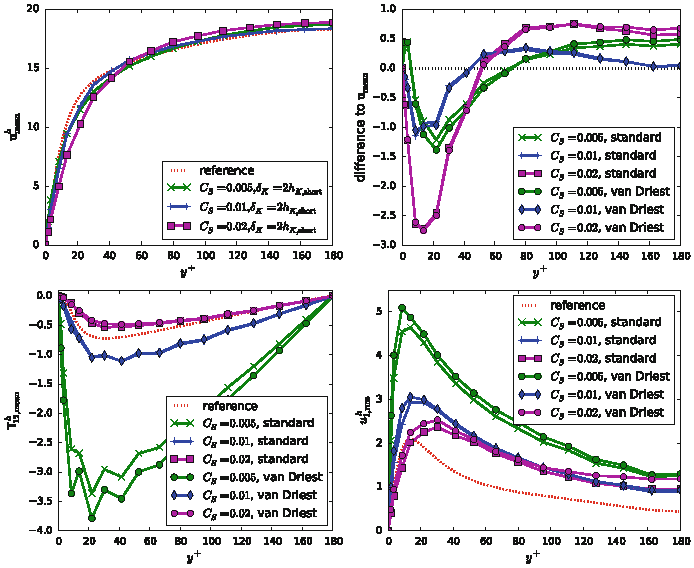
\includegraphics[width=\linewidth]{figures/Chapter_08/Fig_8_11__PDFp648__Bookp639.pdf}
\captionof{figure}{例题\hyperref[ex:vms-coarse-projection-channel-flow]{8.277}:采用 $\mathcal L^H=\mathbb P_0$ 的三尺度粗空间投影 VMS 方法\hyperref[eq:vms-coarse-projection-three-scale-method]{(8.288)}所得的若干统计量.}
\label{fig:vms-channel-p0-statistics}
\end{elegantfigure}

图\hyperref[fig:vms-channel-p0-statistics]{8.11}、\hyperref[fig:vms-channel-p1-statistics]{8.12}和\hyperref[fig:vms-channel-adaptive-statistics]{8.13}分别给出了 $\mathcal L^H=\mathbb P_0$、$\mathcal L^H=\mathbb P_1^{\mathrm{disc}}$ 以及自适应选取投影空间时,三尺度粗空间投影 VMS 方法\hyperref[eq:vms-coarse-projection-three-scale-method]{(8.288)}的结果.

正如笔记\hyperref[note:vms-dynamic-smagorinsky-common-goal]{8.216}所述,三尺度 VMS 方法的目标之一,是限制 Smagorinsky 模型直接作用于小的已解析尺度,从而降低该模型的影响.结果表明,这一目标确已实现:与 Smagorinsky 大涡模拟模型相比,该方法在更宽的 $C_S$ 参数范围内都能给出合理结果,见图\hyperref[fig:smagorinsky-channel-flow]{8.4}.VMS 方法在较大的 $C_S$ 取值下结果最准确.与 Smagorinsky 大涡模拟模型类似,采用 van Driest 阻尼\hyperref[eq:van-driest-damping]{(8.152)}的影响很小.标准 Smagorinsky 方法的结果往往略为准确,但并非总是如此.

\begin{elegantfigure}[1.055\linewidth]
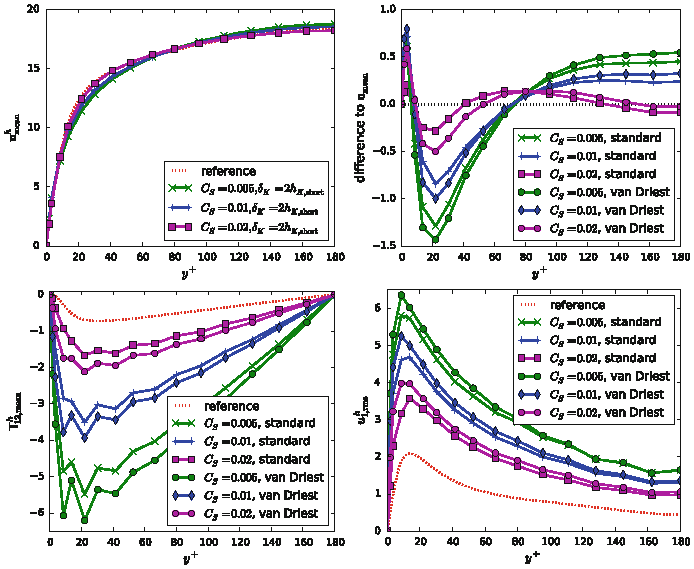
\includegraphics[width=\linewidth]{figures/Chapter_08/Fig_8_12__PDFp649__Bookp640.pdf}
\captionof{figure}{例题\hyperref[ex:vms-coarse-projection-channel-flow]{8.277}:采用 $\mathcal L^H=\mathbb P_1^{\mathrm{disc}}$ 的三尺度粗空间投影 VMS 方法\hyperref[eq:vms-coarse-projection-three-scale-method]{(8.288)}所得的若干统计量.}
\label{fig:vms-channel-p1-statistics}
\end{elegantfigure}

\begin{elegantfigure}[1.055\linewidth]
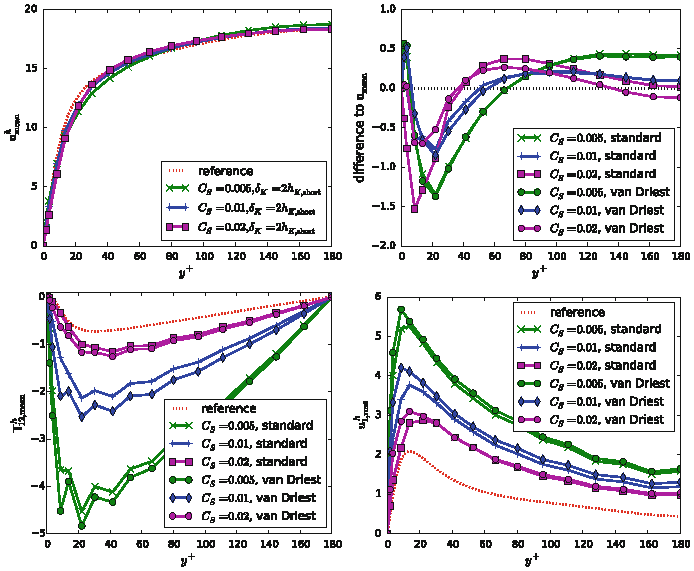
\includegraphics[width=\linewidth]{figures/Chapter_08/Fig_8_13__PDFp650__Bookp641.pdf}
\captionof{figure}{例题\hyperref[ex:vms-coarse-projection-channel-flow]{8.277}:自适应选取投影空间时,三尺度粗空间投影 VMS 方法\hyperref[eq:vms-coarse-projection-three-scale-method]{(8.288)}所得的若干统计量.}
\label{fig:vms-channel-adaptive-statistics}
\end{elegantfigure}
\end{example}
\index{变分多尺度方法!基于粗空间投影!实现}
\index{变分多尺度方法!基于粗空间投影!自适应投影空间}
\index{投影空间!自适应选取}



\section{若干湍流模型的数值比较}
\label{sec:comparison-turbulence-models}

\begin{note}[内容]
\label{note:comparison-turbulence-models-contents}
本节比较本章介绍的若干湍流模型所得到的数值解.重点讨论 Smagorinsky 模型和三尺度粗空间投影 VMS 方法,因为在 $\mathrm{Re}_\tau=180$ 的湍流槽道流中,这两种方法给出的结果最准确.对本节涉及的问题,采用有理 LES 模型、Leray-$\alpha$ 模型和 Navier--Stokes-$\alpha$ 模型进行模拟,通常无法得到令人满意的结果.
\end{note}

\begin{example}[($\mathrm{Re}_\tau=180$ 的湍流槽道流)]
\label{ex:vms-comparison-channel-180}
本例仅列出例题\hyperref[ex:smagorinsky-turbulent-channel]{8.128}和\hyperref[ex:vms-coarse-projection-channel-flow]{8.277}中所考察湍流模型的最佳参数:
\begin{itemize}
 \item Smagorinsky 模型\hyperref[eq:smagorinsky-filter-width]{(8.69)}(Smag):$\delta_K=2h_{K,\mathrm{short}}$,$C_S=0.005$,并采用 van Driest 阻尼\hyperref[eq:van-driest-damping]{(8.152)};
 \item 粗空间投影方法\hyperref[eq:vms-coarse-projection-three-scale-method]{(8.288)},其中 $\mathcal L^H=\mathbb P_0$(VMS0):$\delta_K=2h_{K,\mathrm{short}}$,$C_S=0.01$,不采用 van Driest 阻尼;
 \item 粗空间投影方法\hyperref[eq:vms-coarse-projection-three-scale-method]{(8.288)},其中 $\mathcal L^H=\mathbb P_1^{\mathrm{disc}}$(VMS1):$\delta_K=2h_{K,\mathrm{short}}$,$C_S=0.02$,不采用 van Driest 阻尼;
 \item 自适应选取投影空间的粗空间投影方法(VMSadap):$\delta_K=2h_{K,\mathrm{short}}$,$C_S=0.02$,并采用 van Driest 阻尼\hyperref[eq:van-driest-damping]{(8.152)}.
\end{itemize}
这些参数下的结果见图\hyperref[fig:vms-comparison-channel-180]{8.14}.在所比较的湍流模型中,VMS0 和 VMSadap 的结果最准确,而 Smagorinsky 模型的结果最不准确.

\begin{elegantfigure}[333.25pt]
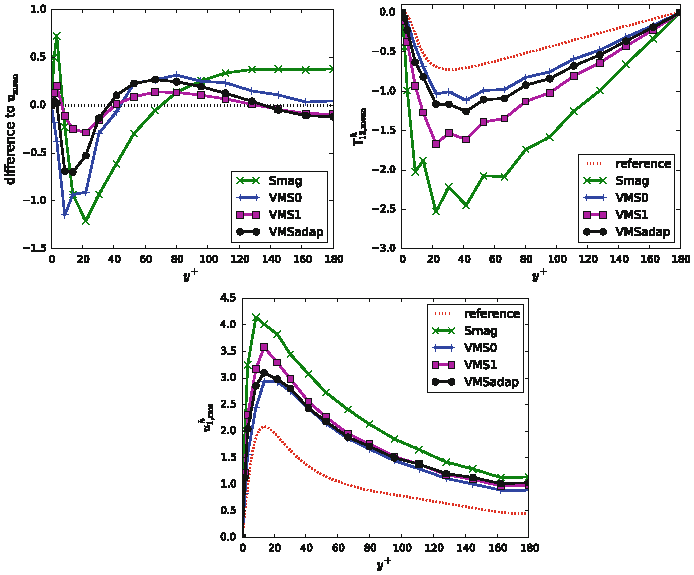
\includegraphics[width=333.25pt]{figures/Chapter_08/Fig_8_14__PDFp651__Bookp642.pdf}
\captionof{figure}{例题\hyperref[ex:vms-comparison-channel-180]{8.279}:$\mathrm{Re}_\tau=180$ 湍流槽道流中,Smagorinsky 模型和三尺度粗空间投影 VMS 模型采用最佳参数时的若干统计量.}
\label{fig:vms-comparison-channel-180}
\end{elegantfigure}
\end{example}

\begin{example}[($\mathrm{Re}_\tau=395$ 的湍流槽道流)]
\label{ex:vms-comparison-channel-395}
本例的说明见例题\hyperref[ex:appendix-d-12]{D.12}.模拟设置与 $\mathrm{Re}_\tau=180$ 的湍流槽道流相似,参见例题\hyperref[ex:smagorinsky-turbulent-channel]{8.128},只是空间网格和时间步长更细.空间网格由 $16\times16\times32$ 个单元组成.对 $Q_2/\mathbb P_1^{\mathrm{disc}}$ 有限元空间对,速度自由度为 199,680 个(包括 Dirichlet 节点),压力自由度为 32,768 个.Crank--Nicolson 格式的时间步长取 $\Delta t=0.002$.时间区间长度、靠近壁面的网格加密等其他设置均与例题\hyperref[ex:smagorinsky-turbulent-channel]{8.128}相同.

结果见图\hyperref[fig:vms-comparison-channel-395]{8.15}.VMS0 配合 $C_S=0.02$ 得到的结果最好.Smagorinsky 模型取 $C_S=0.01$、VMSadap 取 $C_S=0.02$ 时,也得到同样较好的结果.VMS1 取 $C_S=0.01$、Smagorinsky 模型取 $C_S=0.005$ 时,结果不准确.因此,针对 $\mathrm{Re}_\tau=180$ 湍流槽道流选出的 Smagorinsky 模型最佳参数,并不适用于本例.

\begin{elegantfigure}[333.5pt]
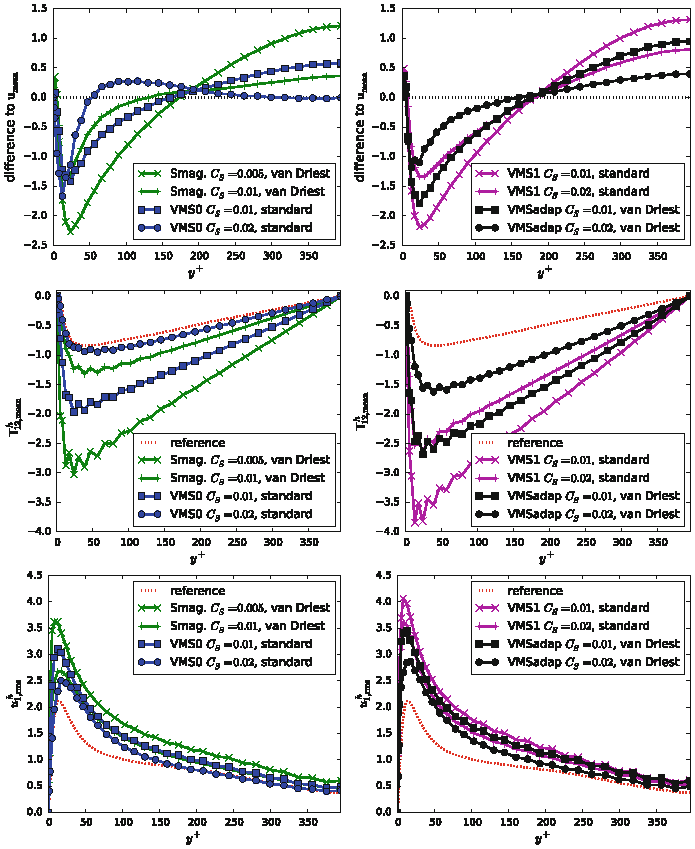
\includegraphics[width=333.5pt]{figures/Chapter_08/Fig_8_15__PDFp652__Bookp643.pdf}
\captionof{figure}{例题\hyperref[ex:vms-comparison-channel-395]{8.280}:$\mathrm{Re}_\tau=395$ 湍流槽道流中,Smagorinsky 模型和三尺度粗空间投影 VMS 模型所得的若干统计量.}
\label{fig:vms-comparison-channel-395}
\end{elegantfigure}
\end{example}

\begin{example}[($\mathrm{Re}=22{,}000$ 的绕圆柱湍流)]
\label{ex:vms-comparison-cylinder}
本例及其关注量见例题\hyperref[ex:appendix-d-13]{D.13}.模拟采用六面体网格和 $Q_2/\mathbb P_1^{\mathrm{disc}}$ 空间对;在第 2 层网格上,速度自由度为 522,720 个(包括 Dirichlet 节点),压力自由度为 81,920 个.图\hyperref[fig:vms-comparison-cylinder-grid]{8.16}给出了初始网格(第 0 层).时间离散采用等距步长 $\Delta t=0.005$ 的 Crank--Nicolson 格式.

\begin{elegantfigure}[226.5pt]
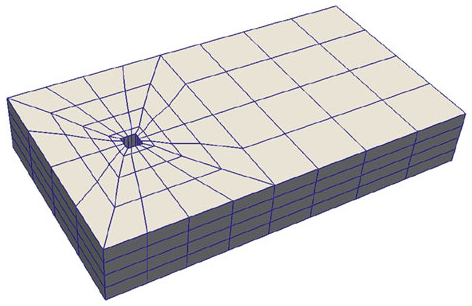
\includegraphics[width=226.5pt]{figures/Chapter_08/Fig_8_16__PDFp653__Bookp644.pdf}
\captionof{figure}{例题\hyperref[ex:vms-comparison-cylinder]{8.281}:初始网格,第 0 层.}
\label{fig:vms-comparison-cylinder-grid}
\end{elegantfigure}

本例不采用 van Driest 阻尼.所有流动均先发展 10 秒,随后在 30 个周期内计算统计量.

\begin{eleganttable}
\centering
\captionof{table}{例题\hyperref[ex:vms-comparison-cylinder]{8.281}}
\label{tab:vms-comparison-cylinder-statistics}
\scriptsize
\setlength{\tabcolsep}{2.5pt}
\renewcommand{\arraystretch}{1.16}
\resizebox{\linewidth}{!}{%
\begin{tabular}{l|c|cc|cc|c}
\hline
方法 & $C_S$ & $c_{\mathrm{lift}}$ & $c_{\mathrm{lift,rms}}$
 & $c_{\mathrm{drag}}$ & $c_{\mathrm{drag,rms}}$ & $\mathrm{St}$\\
\hline
Smag & 0.005 & \multicolumn{5}{c}{计算发散}\\
Smag & 0.01 & 0.001 & 1.46 & 2.58 & 0.11 & 0.151\\
Smag & 0.02 & 0.023 & 1.52 & 2.52 & 0.16 & 0.140\\
VMS0 & 0.01 & $-0.017$ & 1.28 & 2.60 & 0.19 & 0.139\\
VMS0 & 0.02 & $-0.015$ & 1.29 & 2.65 & 0.14 & 0.142\\
VMS1 & 0.01 & $-0.004$ & 1.04 & 2.49 & 0.15 & 0.136\\
VMS1 & 0.02 & $-0.026$ & 1.00 & 2.50 & 0.21 & 0.131\\
VMSadap & 0.01 & $-0.006$ & 1.15 & 2.49 & 0.21 & 0.131\\
VMSadap & 0.02 & $-0.026$ & 1.49 & 2.55 & 0.16 & 0.141\\
实验值 & & 0 & $[0.7,1.4]$ & $[1.9,2.1]$ & $[0.1,0.2]$ & 0.132\\
\hline
\end{tabular}%
}
\par\smallskip
\footnotesize 关注量的计算值及实验值.
\end{eleganttable}

表\hyperref[tab:vms-comparison-cylinder-statistics]{8.1}列出了所比较方法得到的结果.大多数结果在定性上相近:均方根(rms)值处于实验区间内,或仅略微超出该区间;平均阻力系数则明显高于实验值.文献中也经常报告后一现象,例如\textcite{GravemeierKronbichlerGeeWall2011,RasthoferGravemeier2013}.各方法所得 Strouhal 数之间则存在较明显差异:Smagorinsky 模型取 $C_S=0.01$ 时结果最差,VMS1 的结果最好.

\begin{elegantfigure}[226.5pt]
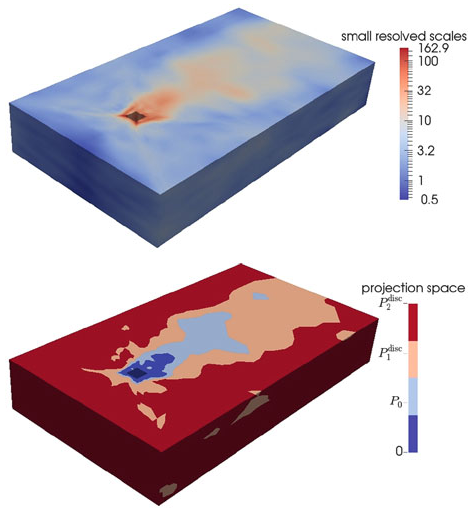
\includegraphics[width=226.5pt]{figures/Chapter_08/Fig_8_17__PDFp654__Bookp645.pdf}
\captionof{figure}{例题\hyperref[ex:vms-comparison-cylinder]{8.281}:自适应投影空间的三尺度投影 VMS 方法中,小的已解析尺度的大小(上)及相应投影空间(下).}
\label{fig:vms-adaptive-cylinder-flow}
\end{elegantfigure}

此外,Smagorinsky 模型取 $C_S=0.005$ 时发散,这一点值得注意.因此,该模型在 $\mathrm{Re}_\tau=180$ 湍流槽道流中的最佳参数在本例中失效.相较之下,本例也表明三尺度粗空间投影 VMS 方法对 $C_S$ 的选取不那么敏感.

图\hyperref[fig:vms-adaptive-cylinder-flow]{8.17}展示了小的已解析尺度的大小、空间分布以及自适应投影空间的相应选取.本例中,圆柱表面及其下游区域的湍流强度预计最高.图中小的已解析尺度的大小与这一预期相符,因此式\hyperref[eq:vms-coarse-projection-local-turbulence-intensity]{(8.328)}中的 $\zeta_K$ 是合适的局部湍流强度估计量.从投影空间图中可以看出,湍流模型在圆柱处的影响最大,沿下游方向逐渐减弱,在其他区域则基本关闭.
\end{example}

\begin{example}[($\mathrm{Re}=40{,}000$ 的壁装立方体绕流)]
\label{ex:vms-comparison-wall-mounted-cube}
本问题见例题\hyperref[ex:appendix-d-14]{D.14}.

\begin{elegantfigure}[226.5pt]
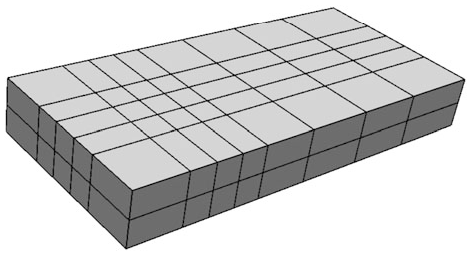
\includegraphics[width=226.5pt]{figures/Chapter_08/Fig_8_18__PDFp655__Bookp646.pdf}
\captionof{figure}{例题\hyperref[ex:vms-comparison-wall-mounted-cube]{8.282}:初始网格,第 0 层.}
\label{fig:vms-comparison-wall-mounted-cube-grid}
\end{elegantfigure}

数值模拟采用六面体网格上的 $Q_2/\mathbb P_1^{\mathrm{disc}}$ 空间对.初始网格(第 0 层)见图\hyperref[fig:vms-comparison-wall-mounted-cube-grid]{8.18},表\hyperref[tab:vms-comparison-wall-mounted-cube-dofs]{8.2}列出了自由度数量.模拟时间区间为 $[0,10]$,时间离散采用等距步长 $\Delta t=0.01$ 的 Crank--Nicolson 格式.计算阻力系数的时间平均值时,取区间 $[5,10]$.所有湍流模型均未采用 van Driest 阻尼.

\begin{eleganttable}[0.68\linewidth]
\centering
\captionof{table}{例题\hyperref[ex:vms-comparison-wall-mounted-cube]{8.282}}
\label{tab:vms-comparison-wall-mounted-cube-dofs}
\scriptsize
\setlength{\tabcolsep}{4pt}
\renewcommand{\arraystretch}{1.12}
\begin{tabular}{c|rrr}
\hline
层级 & 速度 & 压力 & 总计\\
\hline
2 & 134,739 & 20,224 & 154,963\\
3 & 1,023,651 & 161,792 & 1,185,443\\
\hline
\end{tabular}
\par\smallskip
\footnotesize 空间自由度数(包括 Dirichlet 节点).
\end{eleganttable}

\begin{eleganttable}[0.82\linewidth]
\centering
\captionof{table}{例题\hyperref[ex:vms-comparison-wall-mounted-cube]{8.282}}
\label{tab:vms-comparison-wall-mounted-cube-drag}
\scriptsize
\setlength{\tabcolsep}{4pt}
\renewcommand{\arraystretch}{1.12}
\begin{tabular}{l|c|cc}
\hline
方法 & $C_S$ & 第 2 层 & 第 3 层\\
\hline
Smag & 0.005 & 1.16 & 1.46\\
Smag & 0.01 & 1.26 & 1.45\\
VMS0 & 0.01 & 1.19 & 1.47\\
VMS0 & 0.02 & 1.23 & 1.45\\
VMS1 & 0.01 & 1.09 & 1.39\\
VMS1 & 0.02 & 1.11 & 1.38\\
VMSadap & 0.01 & 1.13 & 1.37\\
VMSadap & 0.02 & 1.21 & 1.33\\
\hline
\end{tabular}
\par\smallskip
\footnotesize 平均阻力系数;参考值 $c_{\mathrm{drag}}\approx1.5$.
\end{eleganttable}

表\hyperref[tab:vms-comparison-wall-mounted-cube-drag]{8.3}给出了不同湍流模型的结果.图\hyperref[fig:vms-comparison-wall-mounted-cube-drag]{8.19}以两种模型为例,展示了计算所得阻力系数随时间的变化.可以看到,所有湍流模型在较粗的第 2 层网格上都低估了平均阻力系数.在较细的第 3 层网格上,Smagorinsky 模型和 VMS0 所得平均阻力系数与参考值处于同一量级;VMS1 和 VMSadap 仍明显低估这一系数.图\hyperref[fig:vms-comparison-wall-mounted-cube-drag]{8.19}还表明,在较细网格上,计算阻力系数围绕其平均值的振荡幅度显著减小.

\begin{elegantfigure}[333.25pt]
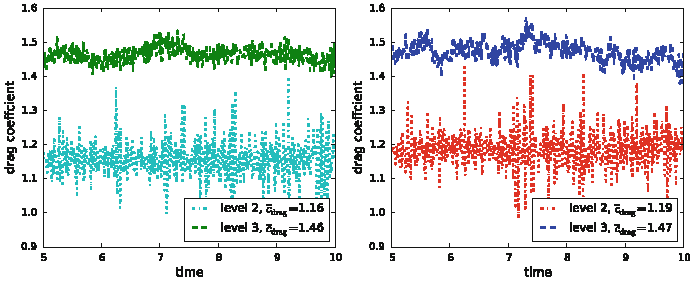
\includegraphics[width=333.25pt]{figures/Chapter_08/Fig_8_19__PDFp656__Bookp647.pdf}
\captionof{figure}{例题\hyperref[ex:vms-comparison-wall-mounted-cube]{8.282}:Smagorinsky 模型 $C_S=0.005$(左)和 VMS0 $C_S=0.01$(右)所得阻力系数.}
\label{fig:vms-comparison-wall-mounted-cube-drag}
\end{elegantfigure}
\end{example}

\index{湍流模型!数值比较}
\index{Smagorinsky 模型!与 VMS 方法比较}
\index{变分多尺度方法!基于粗空间投影!数值比较}


\chapter{耦合线性方程组的求解器}\label{chap:coupled-linear-solvers}

\begin{note}[动机]
\label{note:coupled-solvers-motivation}
许多不可压缩流动模拟方法都需要求解速度与压力耦合的线性问题:
\begin{equation}\label{eq:chapter9-coupled-system}
\mathcal A\,\bm{x}
=\begin{pmatrix}A&D\\B&-C\end{pmatrix}
  \begin{pmatrix}\bm{u}\\p\end{pmatrix}
=\begin{pmatrix}\bm{f}\\f_p\end{pmatrix}
=\bm{y}.
\end{equation}
其中
\[
 A\in\mathbb{R}^{dN_v\times dN_v},\qquad
 D\in\mathbb{R}^{dN_v\times N_p},\qquad
 B\in\mathbb{R}^{N_p\times dN_v},\qquad
 C\in\mathbb{R}^{N_p\times N_p},
\]
\[
 \bm{u},\bm{f}\in\mathbb{R}^{dN_v},\qquad
 p,f_p\in\mathbb{R}^{N_p},
\]
并且
\[
 \mathcal A\in\mathbb{R}^{(dN_v+N_p)\times(dN_v+N_p)},
 \qquad
 \bm{x},\bm{y}\in\mathbb{R}^{dN_v+N_p}.
\]
若 $C=0$,则式\hyperref[eq:chapter9-coupled-system]{(9.1)}是一个线性鞍点问题.对 Navier--Stokes 方程组,尤其是含时问题,往往需要反复求解式\hyperref[eq:chapter9-coupled-system]{(9.1)}这样的系统.高效求解这类系统,是实现不可压缩流动高效数值模拟的核心.
\end{note}

\begin{note}[本章内容]
\label{note:chapter9-contents}
针对式\hyperref[eq:chapter9-coupled-system]{(9.1)}这类问题开发快速求解器,仍是一个活跃的研究领域.\textcite{BenziGolubLiesen2005}综述了这类系统的性质及其经典求解方法.对于不可压缩流动问题离散后得到的式\hyperref[eq:chapter9-coupled-system]{(9.1)},可参见\textcite[第 4、9 章]{Elman2014}和\textcite[第 5.2 节]{OlshanskiiTyrtyshnikov2014}的详细讨论.

本章重点讨论线性鞍点问题,即式\hyperref[eq:chapter9-coupled-system]{(9.1)}中的 $C=0$,并介绍本书数值结果所采用的求解器.此外,也将简要介绍文献中提出的其他一些求解器.
\end{note}

\begin{note}[稀疏矩阵与 CSR 存储格式]
\label{note:chapter9-csr-storage}
各矩阵块都是稀疏矩阵,因此整体矩阵 $\mathcal A$ 也是稀疏的.稀疏矩阵通常采用专门的存储格式,其中压缩稀疏行(compressed sparse row,CSR)格式十分常用.该格式按行存储非零项,无须按列下标排序.

设 $A\in\mathbb{R}^{m\times n}$,其非零项数为 $\mathrm{nnz}$.使用 CSR 格式存储 $A$ 需要三个数组:
\begin{itemize}
  \item 长度为 $\mathrm{nnz}$ 的数组,存储 $A$ 的非零项;
  \item 长度为 $\mathrm{nnz}$ 的整数数组,存储前一个数组中各项对应的列下标;
  \item 长度为 $m+1$ 的整数数组,其中第 $i$ 项指出第 $i$ 行在前两个数组中的起始位置;最后一项指出第 $m+1$ 行本应开始的位置.
\end{itemize}
对于不可压缩流问题,常见做法是将 $\mathcal A$ 中的 $A$、$B$、$D$ 各块分别按这种格式存储.
\end{note}

\begin{note}[系统矩阵的若干性质]
\label{note:chapter9-system-matrix-properties}
在许多问题中,系统矩阵具有比式\hyperref[eq:chapter9-coupled-system]{(9.1)}更特殊的形式,或者某些矩阵块具有特殊性质.对于满足 inf-sup 条件的有限元空间,采用 Galerkin 有限元法时有 $C=0$ 且 $D=B^{\mathsf T}$;后一性质还取决于具体问题的边界条件.对于 Stokes 方程,矩阵块 $A$ 是对称的.通常 $C$ 也对称,例如在压力稳定化 Petrov--Galerkin(PSPG)方法中.
\end{note}

\section{耦合问题的求解器}\label{sec:chapter9-coupled-solvers}

\begin{note}[稀疏直接求解器]
\label{note:chapter9-solver-choice}\label{note:umfpack}\label{note:ch09-sparse-direct-solvers}
稀疏线性方程组最容易采用直接求解器求解,这类方法称为稀疏直接求解器.常用软件包括:
\begin{itemize}
  \item MUMPS,\textcite{Amestoy2001,Amestoy2006};
  \item PARDISO,\textcite{Schenk2008};
  \item UMFPACK,\textcite{Davis2004}.
\end{itemize}
对于二维问题以及自由度较少或中等规模(约不超过 $500{,}000$ 个自由度)的问题,这些求解器尤其高效.不过,对于三维问题,它们往往效率较低,参见笔记\hyperref[note:time-dependent-picard-newton-comparison]{7.56}及例题\hyperref[ex:time-dependent-picard-vs-newton]{7.57}.这是由二维和三维离散矩阵的稀疏结构不同造成的:三维问题中的内部自由度通常比二维问题有更多相邻自由度,因而矩阵项更多、稀疏程度更低.稀疏直接求解器试图在矩阵分解中尽量减少填充;矩阵越稀疏,通常越容易做到这一点.

直接求解器无法利用已有的良好近似解.对于时间依赖问题,若时间步不太大,前一离散时刻的解或由多个先前时刻的解外推得到的结果,通常都能较好地近似当前时刻的解;此时直接求解器无法利用这一优势.

数值线性代数研究表明,对于病态问题,直接求解器所得结果可能不够准确.此时建议再用迭代方法作后处理,以提高精度.
\end{note}

\begin{note}[迭代求解器与 Krylov 子空间方法]
\label{note:chapter9-iterative-solvers}
\label{note:chapter9-multigrid-preconditioner}
设 $\bm r\in\mathbb{R}^{dN_v+N_p}$.对整数 $k\ge 1$,定义
\[
 \mathcal K_k(\bm r,\mathcal A)
 :=\operatorname{span}\{\bm r,\mathcal A\bm r,\ldots,
              \mathcal A^{k-1}\bm r\}.
\]
称这一空间为由 $\bm r$ 和 $\mathcal A$ 张成的 $k$ 维 Krylov 子空间.

求解式\hyperref[eq:chapter9-coupled-system]{(9.1)}的常用迭代方法属于 Krylov 子空间方法.设 $\bm{x}^{(0)}$ 是式\hyperref[eq:chapter9-coupled-system]{(9.1)}解的一个初始近似,则残量向量为
\[
 \bm r^{(0)}=\bm y-\mathcal A\bm x^{(0)}.
\]
相应地,考察子空间 $\mathcal K_k(\bm r^{(0)},\mathcal A)$.

\begin{itemize}
  \item \textbf{GMRES 与 FGMRES.} GMRES(generalized minimal residual,广义最小残量)方法由\textcite{SaadSchultz1986}提出.它在仿射空间 $\bm{x}^{(0)}+\mathcal K_k(\bm r^{(0)},\mathcal A)$ 中选取第 $k$ 次迭代,使残量向量的欧几里得范数最小.其优点是残量范数不会增大,因而可以直接监控;缺点是必须存储整个 Krylov 子空间的一组基.通常只有在 $k$ 较小时,这种存储需求才可接受.此外,每次迭代的运算量会随迭代次数增加.实践中常把最大迭代次数 $k$ 设为 $10$ 至 $100$.若迭代 $k$ 步后仍未收敛,就以当前迭代值为初值重新启动;这种策略称为重启 GMRES,记作 GMRES(restart).

  如第\hyperref[sec:chapter9-preconditioners]{9.2 节}所述,通常需要采用预条件子加快收敛.若预条件子不是固定矩阵,而是一种数值方法,则应采用\textcite{Saad1993}提出的灵活 GMRES(flexible GMRES,FGMRES)方法.数值方法的作用可以用一个矩阵表示;这个矩阵通常未知,而且可能随迭代而改变.FGMRES 能够处理迭代过程中预条件子的变化,但需要存储两个 Krylov 子空间的基,因此内存需求更高.

  \item \textbf{CGS.} CGS(conjugate gradient squared,平方共轭梯度)由\textcite{Sonneveld1989}提出.其基本思想是计算第 $k$ 次迭代,使残量向量与子空间 $\mathcal K_k(\bm r^{(0)},\mathcal A^{\mathsf T})$ 正交.CGS 是这一思想的一种实现,不需要显式知道 $\mathcal A^{\mathsf T}$.该方法可采用所谓短递推实现,即只需少量数组,且迭代过程中所需数组数量不增加.因此,它的内存需求远低于 GMRES.不过,CGS 不会使残量向量的欧几里得范数最小,该范数在迭代中甚至可能大幅增大,所以收敛过程可能不规则.

  \item \textbf{BiCGStab.} BiCGStab(bi-conjugate gradient stabilized,稳定双共轭梯度)方法由\textcite{VanDerVorst1992}提出,其依据与 CGS 相同;它是 CGS 的一种改进,通常更加稳定.
\end{itemize}

要加快迭代求解器的收敛,必须采用预条件子,参见第\hyperref[sec:chapter9-preconditioners]{9.2 节}.提供适用于线性鞍点问题的迭代求解器和预条件子的程序库包括 PETSc(\textcite{Balay2016})和 Trilinos(\textcite{Trilinos2016}).
\end{note}

\begin{note}[迭代求解式(9.1)的策略]
\label{note:chapter9-inexact-strategy}
对于 Navier--Stokes 方程组,式\hyperref[eq:chapter9-coupled-system]{(9.1)}这样的系统会出现在 Picard 迭代或 Newton 迭代中,参见第\hyperref[sec:steady-ns-iterations]{6.3 节}.经验表明,使用迭代求解器时,若将式\hyperref[eq:chapter9-coupled-system]{(9.1)}求解到很高精度,往往效率不高.因此通常采用非精确求解:将最大迭代次数设得较小,或者要求残量向量的欧几里得范数达到较小的缩减因子,例如降至 $10^{-1}$,从而获得一位有效数字.满足任一停止准则后,就进入下一步 Picard 或 Newton 迭代.这一策略的性能见例题\hyperref[ex:steady-ns-picard-vs-newton]{6.47}和例题\hyperref[ex:time-dependent-picard-vs-newton]{7.57}.
\end{note}

\index{稀疏矩阵}
\index{压缩稀疏行(CSR)存储格式}
\index{稀疏直接求解器}
\index{Krylov 子空间方法}
\index{GMRES}
\index{灵活 GMRES(FGMRES)}
\index{CGS}
\index{BiCGStab}
\index{线性鞍点问题!迭代求解器}

\section{迭代求解器的预条件子}\label{sec:chapter9-preconditioners}

\begin{note}[预条件子]
\label{note:chapter9-preconditioners}
众所周知,采用预条件子可以显著改善迭代求解器的性能.预条件子是对 $\mathcal A^{-1}$ 的近似,且能够以相对较低的计算代价求得.这种近似可以是一个固定矩阵、一种数值(迭代)方法,或二者的组合.

预条件分为左预条件和右预条件.记预条件子为 $M^{-1}$.对于左预条件,迭代求解器求解的系统由式\hyperref[eq:chapter9-coupled-system]{(9.1)}改为
\[
 M^{-1}\mathcal A\bm x=M^{-1}\bm y.
\]
采用右预条件时,迭代求解器求解
\[
 \mathcal A M^{-1}\bm z=\bm y,
 \qquad \bm x=M^{-1}\bm z.
\]
同一迭代求解器配合同一预条件子,采用左预条件和右预条件时的表现可能不同.例如,左、右预条件 GMRES 最小化的残量不同;详见\textcite[第 9.3.4 节]{Saad2003}.
\end{note}



\subsection{不完全分解}\label{subsec:chapter9-incomplete-factorizations}

\begin{note}[不完全分解]
\label{note:chapter9-incomplete-factorizations}
对稀疏矩阵 $\mathcal A$ 作 LU 分解时,所得因子 $L$ 和 $U$ 通常会比 $\mathcal A$ 稠密得多.在不完全 LU 分解(incomplete LU factorization,ILU)中,$L$ 和 $U$ 保留与 $\mathcal A$ 相同的稀疏结构:$L$ 的稀疏结构对应于 $\mathcal A$ 的严格下三角部分,$U$ 的稀疏结构对应于 $\mathcal A$ 的上三角部分.执行不带主元选取的标准 LU 分解算法时,舍弃所有不符合预定稀疏结构的项,由此得到不完全分解
\begin{equation}\label{eq:chapter9-ilu-incomplete-factorization}
 \mathcal A=LU+E,
\end{equation}
其中 $E$ 为误差矩阵.

例如,\textcite{DahlWille1992}指出,对 $\mathcal A$ 作 ILU 分解时不采用主元选取,并不一定会导致算法失败.首先,应按压力自由度排在最后的方式排列自由度,这与式\hyperref[eq:chapter9-coupled-system]{(9.1)}中的排列一致.其次,需要给定稀疏矩阵 $C$,其稀疏结构应包含压力自由度之间的全部连接(与 inf-sup 稳定化方法中的情形相同),并将 $C$ 的所有项初始化为零.在这两个条件下,\textcite{DahlWille1992}观察到,不完全分解过程中主对角线上的零项会消失,因此不会发生除以零.

所谓 ILUT$(l,\tau)$ 方法(\textcite[第 10.4.1 节]{Saad2003})允许保留 LU 分解中模大于阈值 $\tau\ge0$ 的项,即使这些项不符合原有稀疏结构.对于当前行,只保留 $L$ 部分中按绝对值计最大的 $l$ 项、$U$ 部分中按绝对值计最大的 $l$ 项,另加对角项.这样得到式\hyperref[eq:chapter9-ilu-incomplete-factorization]{(9.2)}形式的不完全分解;其误差矩阵的非零项预计会更小,同时避免完整 LU 分解产生的全部填充.
\end{note}

\begin{note}[带填充的不完全 LU 预条件子]
\label{note:chapter9-ilu-fill-in}
\textcite{Konshin2015}提出了一种 ILU 预条件子,用于求解非定常 Navier--Stokes 方程组离散后产生的线性鞍点问题.该预条件子对整体矩阵 $\mathcal A$ 作不带主元选取的分解,其形式为
\[
 \mathcal A=LU+L R_u+R_l U+E,
\]
其中 $R_u$ 为严格上三角矩阵,$R_l$ 为严格下三角矩阵,$E$ 仍为误差矩阵.给定两个参数 $\tau_1\ge\tau_2>0$,构造分解时要求 $L$ 和 $U$ 的非对角项要么为零,要么其绝对值大于 $\tau_1$;而 $R_u$ 和 $R_l$ 的非对角项要么为零,要么其绝对值属于 $(\tau_2,\tau_1]$.因此,误差矩阵 $E$ 中的项为 $O(\tau_2)$.如\textcite{Konshin2015}所述,该方法的填充量由 $\tau_1$ 决定;当 $\tau_2=O(\tau_1)$ 时,所得预条件子的质量则由 $\tau_2$ 控制.

要使该预条件子高效工作,首先需要对矩阵 $\mathcal A$ 进行适当缩放.\textcite{Konshin2015}表明,选取合适的 $\tau_1$ 和 $\tau_2$ 后,该预条件子可用于一大类黏度下的层流三维非定常 Navier--Stokes 问题,并能高效求解.
\end{note}

\index{预条件子!左预条件}
\index{预条件子!右预条件}
\index{不完全 LU 分解(ILU)}
\index{不完全 LU 预条件子!带填充}

\subsection{耦合多重网格方法}
\label{subsec:chapter9-coupled-multigrid}\label{subsec:multigrid-method}
\label{subsec:chapter9-iterative-solvers}

\begin{note}[多重网格方法]
\label{note:chapter9-multigrid-methods}\label{note:multigrid-method}
多重网格方法通过一系列网格层级求解线性方程组.在每一层上,都近似求解相应的方程;只有在最粗层(称为第 0 层)上,方程才可能被高精度求解.多重网格方法需要在相邻层级之间传递信息:由细层向粗层传递称为限制,由粗层向细层传递称为延拓.关于多重网格方法的介绍可参见\textcite{Hackbusch1985,Trottenberg2001,Briggs2000}.

下面介绍用于求解式\hyperref[eq:chapter9-coupled-system]{(9.1)}的多重网格方法的组成部分.该方法同时求解速度 $\bm u$ 和压力 $p$ 两类未知量,因而称为耦合多重网格方法.它由以下部分定义:
\begin{itemize}
  \item 网格层级,见笔记\hyperref[note:chapter9-grid-hierarchy]{9.12};
  \item 粗层系统矩阵的定义,见笔记\hyperref[note:chapter9-coarse-system-matrices]{9.13};
  \item 网格间传递算子:
  \begin{itemize}
    \item 函数延拓,见笔记\hyperref[note:chapter9-function-prolongation]{9.14};
    \item 缺陷限制,见笔记\hyperref[note:chapter9-defect-restriction]{9.18};
    \item 函数限制,见笔记\hyperref[note:chapter9-function-restriction]{9.19};
  \end{itemize}
  \item 细层上的光滑子,见笔记\hyperref[note:chapter9-vanka-smoother]{9.20};
  \item 粗网格求解器,见笔记\hyperref[note:chapter9-coarse-grid-solver]{9.24}.
\end{itemize}
\end{note}

\index{多重网格方法}


\begin{note}[网格层级]
\label{note:chapter9-grid-hierarchy}
定义多重网格层级有多种方式.标准做法是沿用几何网格的层级,并在各层上采用相同的离散方法.不过,多重网格层级也可以多于几何网格层级,并且粗层可采用不同于最细层的离散方法.图\hyperref[fig:chapter9-multigrid-approaches]{9.1}所示的多重离散多层方法就是一例.

\begin{elegantfigure}[333.25pt]

\includegraphics[page=663,pagebox=cropbox,trim=53.00bp 464.15bp 53.11bp 61.50bp,clip,width=333.25pt]{../input/source/Finite Element Methods for Incompressible Flow Problems.pdf}
\captionof{figure}{标准多重网格方法(左)与面向高阶离散的多重离散多层方法(右).}
\label{fig:chapter9-multigrid-approaches}
\end{elegantfigure}

在\textcite{JohnMatthies2001}关于例题\hyperref[ex:appendix-d-5]{D.5}以及\textcite{John2002}关于例题\hyperref[ex:appendix-d-6]{D.6}的数值研究中,研究者发现:对于某些高阶有限元离散所得的线性鞍点问题,标准多重网格方法会遇到困难.高阶有限元离散能够较准确地计算感兴趣量,参见例题\hyperref[ex:steady-ns-flow-around-cylinder]{6.36}.与此相反,带迎风稳定化的最低阶非协调离散的精度较低,参见笔记\hyperref[note:oseen-upwind-nonconforming]{5.58};但标准多重网格方法已被证明是一种效率很高的求解器,另见\textcite{JohnTobiska2000}.由此产生了一个构造高阶有限元离散多层方法的思路:以稳定的最低阶非协调有限元离散所用的多层方法为基础.这就是图\hyperref[fig:chapter9-multigrid-approaches]{9.1}所示的多重离散多层方法.

该方法的多层层级比几何网格层级多一层.在最细的几何网格(第 $L$ 层)上采用两种离散方法:其中一种是所关注的高阶离散,它构成多层层级的最细层;另一种是在几何第 $L$ 层上采用带迎风稳定化的最低阶非协调离散.在所有更粗的几何层上,也采用经过稳定化的最低阶非协调离散.

在多重网格方法中,网格序列的组织方式称为循环.最常见的多重网格循环见图\hyperref[fig:chapter9-multigrid-cycles]{9.2}.

\begin{elegantfigure}[333.25pt]

\includegraphics[page=664,pagebox=cropbox,trim=53.00bp 416.15bp 53.11bp 61.00bp,clip,width=333.25pt]{../input/source/Finite Element Methods for Incompressible Flow Problems.pdf}
\captionof{figure}{多重网格 V 循环、F 循环和 W 循环(依次为左上、右上和下图);$s$ 表示光滑,$r$ 表示限制,$p$ 表示延拓,$e$ 表示精确求解器.}
\label{fig:chapter9-multigrid-cycles}
\end{elegantfigure}
从浮点运算次数看,V 循环代价最低,W 循环代价最高;从稳定性看,情况正好相反.F 循环通常是在计算代价与稳定性之间折中的一种选择.
\end{note}

\index{多重网格方法!V 循环}
\index{多重网格方法!F 循环}
\index{多重网格方法!W 循环}
\index{多层方法!多重离散}


\begin{note}[粗层线性系统的定义]
\label{note:chapter9-coarse-system-matrices}
所谓 Galerkin 投影利用第 $l$ 层的系统矩阵以及延拓、限制算子,定义第 $l-1$ 层的系统矩阵.然而,这种方法无法在不同层级上使用不同的离散方法,而后者正是多重离散多层方法的核心思想.此外,从实现角度看,在粗层上直接组装系统矩阵、并采用与最细层相同的组装方式,似乎更为简便.因此,实际中常采用直接组装.
\end{note}

\begin{note}[函数延拓]
\label{note:chapter9-function-prolongation}
多重网格方法需要将有限元函数从某一层级传递到紧邻的更细层.在多重离散多层方法中,相邻层上的有限元空间可能并不嵌套,因此传递算子必须能够处理这种情形.\textcite{Schieweck2000}提出并分析了一种可在几乎任意有限元空间之间传递函数的算子.下面以标量有限元函数为例,较详细地介绍这一算子.它基于节点泛函的概念(见笔记\hyperref[note:appendix-b-18]{B.18})和局部基(见笔记\hyperref[note:appendix-b-20]{B.20}).

考虑从有限元空间 $V_{l-1}^h$ 到有限元空间 $V_l^h$ 的传递(延拓).设 $\mathcal T_{l-1}$ 和 $\mathcal T_l$ 分别为相应的区域剖分,其中 $\mathcal T_l$ 由 $\mathcal T_{l-1}$ 加密得到,或者 $\mathcal T_l=\mathcal T_{l-1}$.后一种情形适用于多重离散多层方法中的 $l=L+1$,见图\hyperref[fig:chapter9-multigrid-approaches]{9.1}.

设 $S_l^h$ 是定义在 $\mathcal T_l$ 上的不连续有限元空间:
\[
 S_l^h=\left\{w\in L^2(\Omega):
     w|_K\in S_l^h(K)\quad\forall K\in\mathcal T_l\right\}.
\]
局部空间 $S_l^h(K)$ 的选取取决于 $V_{l-1}^h$ 和 $V_l^h$,并须满足包含关系
\begin{equation}\label{eq:chapter9-transfer-space-inclusion}
 V_{l-1}^h+V_l^h\subseteq S_l^h.
\end{equation}
从实际实现角度看,构造传递算子时并不需要用到局部空间 $S_l^h(K)$.从理论角度看,可以证明,对于由单形构成的剖分,总能找到适当的 $S_l^h(K)$,见\textcite{JohnKnoblochMatthiesTobiska2002}.

利用整体节点泛函(见笔记\hyperref[note:appendix-b-23]{B.23}),延拓传递算子定义为
\begin{equation}\label{eq:chapter9-function-prolongation}
 P_{l-1}^{l}:S_l^h\longrightarrow V_l^h,
 \qquad
 P_{l-1}^{l}w=\sum_{i=1}^{\dim(V_l^h)}N_{l,i}(w)\,\varphi_{l,i}^h,
\end{equation}
其中 $\{\varphi_{l,i}^h\}_{i=1}^{\dim(V_l^h)}$ 是 $V_l^h$ 的有限元基,$N_{l,i}$ 是第 $l$ 层的整体节点泛函,满足
\[
 N_{l,i}(\varphi_{l,j}^h)=\delta_{ij}.
\]
由包含关系\hyperref[eq:chapter9-transfer-space-inclusion]{(9.3)}可知,算子\hyperref[eq:chapter9-function-prolongation]{(9.4)}特别适用于 $V_{l-1}^h$ 中的函数.
\end{note}

\begin{note}[用局部泛函计算整体泛函]
\label{note:chapter9-local-functionals}
设 $\{\varphi_{l-1,i}^h\}_{i=1}^{\dim(V_{l-1}^h)}$ 是 $V_{l-1}^h$ 的有限元基,并令
\[
 w_{l-1}^h=\sum_{i=1}^{\dim(V_{l-1}^h)}w_{l-1,i}\,\varphi_{l-1,i}^h
 \in V_{l-1}^h.
\]
要计算将 $w_{l-1}^h$ 延拓时 $\varphi_{l,i}^h$ 的系数,需计算
\[
\begin{aligned}
 N_{l,i}(w_{l-1}^h)
 &=\frac{1}{\operatorname{card}(\mathcal T_{l,i})}
   \sum_{K\in\mathcal T_{l,i}}
   N_{l,i}^K\!\left(w_{l-1}^h|_K\right)\\
 &=\frac{1}{\operatorname{card}(\mathcal T_{l,i})}
   \sum_{K\in\mathcal T_{l,i}}\sum_{j=1}^{\dim(V_{l-1}^h)}
   w_{l-1,j}\,
   N_{l,i}^K\!\left(\varphi_{l-1,j}^h|_K\right),
\end{aligned}
\]
其中 $\mathcal T_{l,i}$ 表示与第 $l$ 层第 $i$ 个节点相关联的网格单元,$N_{l,i}^K$ 是单元 $K$ 上相应的局部节点泛函.
\end{note}

\begin{elegantfigure}[226.5pt]

\includegraphics[page=666,pagebox=cropbox,trim=106.00bp 525.40bp 106.86bp 61.75bp,clip,width=226.5pt]{../input/source/Finite Element Methods for Incompressible Flow Problems.pdf}
\captionof{figure}{红色加密三角形网格,$P_1(P(K))\to P_1(K)$.}
\label{fig:chapter9-red-refined-p1}
\end{elegantfigure}

\begin{example}[(局部泛函的计算)]
\label{ex:chapter9-local-functional-evaluation}
下面详细说明计算 $N_{l,i}^K\bigl(\varphi_{l-1,j}^h|_K\bigr)$ 的几种具体情形.为简便起见,只讨论二维有限元.设 $P(K)\in\mathcal T_{l-1}$ 是 $K\in\mathcal T_l$ 的父网格单元.图\hyperref[fig:chapter9-red-refined-p1]{9.3}--\hyperref[fig:chapter9-rotated-q1-q2]{9.6}中以圆圈表示 $P(K)$ 的局部自由度,以方块表示 $K$ 的局部自由度.

\begin{itemize}
\item \textbf{红色加密三角形:$P_1(P(K))\to P_1(K)$.} 考虑图\hyperref[fig:chapter9-red-refined-p1]{9.3}所示的两种情形.对这一有限元,局部节点泛函是点值,因此 $N_{l,i}^K\bigl(\varphi_{l-1,j}^h|_K\bigr)$ 等于 $\varphi_{l-1,j}^h$ 在 $K$ 中第 $i$ 个局部自由度位置处的取值.所得数值如下:

\begin{eleganttable}[0.84\linewidth]
\centering
\scriptsize
\setlength{\tabcolsep}{4pt}
\renewcommand{\arraystretch}{1.08}
\begin{tabular}{c|ccc|ccc}
\multicolumn{1}{c}{} & \multicolumn{3}{c|}{图\hyperref[fig:chapter9-red-refined-p1]{9.3} 左图} & \multicolumn{3}{c}{图\hyperref[fig:chapter9-red-refined-p1]{9.3} 右图}\\
 & $\varphi_{l-1,0}^h$ & $\varphi_{l-1,1}^h$ & $\varphi_{l-1,2}^h$ & $\varphi_{l-1,0}^h$ & $\varphi_{l-1,1}^h$ & $\varphi_{l-1,2}^h$\\
\hline
$N_{l,0}^K$ & $1$ & $0$ & $0$ & $\tfrac12$ & $\tfrac12$ & $0$\\
$N_{l,1}^K$ & $\tfrac12$ & $\tfrac12$ & $0$ & $0$ & $\tfrac12$ & $\tfrac12$\\
$N_{l,2}^K$ & $\tfrac12$ & $0$ & $\tfrac12$ & $\tfrac12$ & $0$ & $\tfrac12$\\
\end{tabular}
\end{eleganttable}

可见,这种延拓就是标准的包含算子.

\item \textbf{红色加密三角形:$P_1^{\mathrm{nc}}(P(K))\to P_1^{\mathrm{nc}}(K)$.} 再考虑图\hyperref[fig:chapter9-red-refined-p1-nc]{9.4}所示的两种情形.此时,局部节点泛函是 $K$ 各边上的积分平均值.例如,
\[
 N_{l,0}^K\!\left(\varphi_{l-1,j}^h|_K\right)
 =\frac{1}{\|x_0-x_1\|_2}
   \int_{x_0}^{x_1}\varphi_{l-1,j}^h|_K\,\mathrm ds.
\]
所得局部节点泛函数值如下:

\begin{eleganttable}[0.84\linewidth]
\centering
\scriptsize
\setlength{\tabcolsep}{4pt}
\renewcommand{\arraystretch}{1.08}
\begin{tabular}{c|ccc|ccc}
\multicolumn{1}{c}{} & \multicolumn{3}{c|}{图\hyperref[fig:chapter9-red-refined-p1-nc]{9.4} 左图} & \multicolumn{3}{c}{图\hyperref[fig:chapter9-red-refined-p1-nc]{9.4} 右图}\\
 & $\varphi_{l-1,0}^h$ & $\varphi_{l-1,1}^h$ & $\varphi_{l-1,2}^h$ & $\varphi_{l-1,0}^h$ & $\varphi_{l-1,1}^h$ & $\varphi_{l-1,2}^h$\\
\hline
$N_{l,0}^K$ & $1$ & $-\tfrac12$ & $\tfrac12$ & $\tfrac12$ & $\tfrac12$ & $0$\\
$N_{l,1}^K$ & $\tfrac12$ & $0$ & $\tfrac12$ & $0$ & $\tfrac12$ & $\tfrac12$\\
$N_{l,2}^K$ & $\tfrac12$ & $-\tfrac12$ & $1$ & $\tfrac12$ & $0$ & $\tfrac12$\\
\end{tabular}
\end{eleganttable}

\begin{elegantfigure}[225.75pt]

\includegraphics[page=667,pagebox=cropbox,trim=106.50bp 536.40bp 107.11bp 60.25bp,clip,width=225.75pt]{../input/source/Finite Element Methods for Incompressible Flow Problems.pdf}
\captionof{figure}{红色加密三角形网格,$P_1^{\mathrm{nc}}(P(K))\to P_1^{\mathrm{nc}}(K)$.}
\label{fig:chapter9-red-refined-p1-nc}
\end{elegantfigure}

将这些局部节点泛函代入延拓算子\hyperref[eq:chapter9-function-prolongation]{(9.4)},便得到标准的平均算子,见图\hyperref[fig:chapter9-prolongation-weights]{9.5}.图中方块表示待计算的 $V_l^h$ 自由度,圆圈表示 $V_{l-1}^h$ 的节点;标注的数值是对 $V_{l-1}^h$ 中相应节点处函数系数所用的权重.可以看到,图\hyperref[fig:chapter9-prolongation-weights]{9.5}左图中的延拓值,正是 $V_{l-1}^h$ 中有限元函数在该点的取值:将此函数限制到 $\mathcal T_{l-1}$ 中相邻三角形后,所得取值取平均即可.

\begin{elegantfigure}[226.25pt]

\includegraphics[page=667,pagebox=cropbox,trim=106.00bp 399.90bp 107.11bp 158.75bp,clip,width=226.25pt]{../input/source/Finite Element Methods for Incompressible Flow Problems.pdf}
\captionof{figure}{红色加密三角形网格上,$P_1^{\mathrm{nc}}(P(K))\to P_1^{\mathrm{nc}}(K)$ 延拓所用的权重.}
\label{fig:chapter9-prolongation-weights}
\end{elegantfigure}

\item \textbf{未加密的仿射映射四边形:$Q_{\mathrm{rot}}^1(P(K))\to Q_2(K)$.} 此时 $P(K)=K$.首先在 $Q_{\mathrm{rot}}^1(\widehat K)$ 中更换基.容易验证,式\hyperref[eq:appendix-b-22]{(B.22)}给出的 $Q_{\mathrm{rot}}^1(\widehat K)$ 局部基满足
\[
 \frac{1}{|\widehat E_i|}
 \int_{\widehat E_i}\widehat\varphi_j^h\,\mathrm ds
 =\delta_{ij},
\]
其中参考单元的边 $\widehat E_i$ 按逆时针方向编号,从底边开始.设 $K$ 是具有仿射参考变换的任意网格单元,且参考单元上的点 $(\widehat x_1,\widehat x_2)\in\widehat K$ 经映射后对应到 $K$ 中的点 $(x_1,x_2)$.相应基函数满足变换关系
\[
 \widehat\varphi^h(\widehat x_1,\widehat x_2)
 =\varphi^h(x_1,x_2).
\]
因此,只需在参考单元上计算基函数取值,就能方便地得到变换后基函数在 $K$ 上的取值.仿射参考变换对应图\hyperref[fig:chapter9-rotated-q1-q2]{9.6}所示情形.$Q_2(K)$ 的局部节点泛函定义为 $Q_{\mathrm{rot}}^1(\widehat K)$ 局部基函数的点值.如前所述,这些点值可在参考单元 $\widehat K$ 上计算,所得结果与 $K$ 无关:

\begin{eleganttable}[0.84\linewidth]
\centering
\scriptsize
\setlength{\tabcolsep}{5pt}
\renewcommand{\arraystretch}{1.06}
\begin{tabular}{c|rrrr}
 & $\varphi_{l-1,0}^h|_K$ & $\varphi_{l-1,1}^h|_K$ & $\varphi_{l-1,2}^h|_K$ & $\varphi_{l-1,3}^h|_K$\\
\hline
$N_{l,0}^K$ & $\tfrac34$ & $-\tfrac14$ & $-\tfrac14$ & $\tfrac34$\\
$N_{l,1}^K$ & $\tfrac98$ & $-\tfrac18$ & $\tfrac18$ & $-\tfrac18$\\
$N_{l,2}^K$ & $\tfrac34$ & $\tfrac34$ & $-\tfrac14$ & $-\tfrac14$\\
$N_{l,3}^K$ & $-\tfrac18$ & $\tfrac18$ & $-\tfrac18$ & $\tfrac98$\\
$N_{l,4}^K$ & $\tfrac14$ & $\tfrac14$ & $\tfrac14$ & $\tfrac14$\\
$N_{l,5}^K$ & $-\tfrac18$ & $\tfrac98$ & $-\tfrac18$ & $\tfrac18$\\
$N_{l,6}^K$ & $-\tfrac14$ & $-\tfrac14$ & $\tfrac34$ & $\tfrac34$\\
$N_{l,7}^K$ & $\tfrac18$ & $-\tfrac18$ & $\tfrac98$ & $-\tfrac18$\\
$N_{l,8}^K$ & $-\tfrac14$ & $\tfrac34$ & $\tfrac34$ & $-\tfrac14$\\
\end{tabular}
\end{eleganttable}

\begin{elegantfigure}[160.25pt]

\includegraphics[page=668,pagebox=cropbox,trim=139.50bp 485.65bp 139.61bp 61.75bp,clip,width=160.25pt]{../input/source/Finite Element Methods for Incompressible Flow Problems.pdf}
\captionof{figure}{未加密的仿射映射四边形,$Q_{\mathrm{rot}}^1(P(K))\to Q_2(K)$.}
\label{fig:chapter9-rotated-q1-q2}
\end{elegantfigure}

实际计算中,双线性参考映射的情形也采用同一组数值.上述例子表明,局部节点泛函 $N_{l,i}^K\bigl(\varphi_{l-1,j}^h|_K\bigr)$ 的取值通常会在许多网格单元上重复出现.因此,可以在预处理阶段预先计算并存入数据库.计算延拓时,只需利用这些数值进行局部矩阵--向量乘法.采用这一策略可以加速延拓算子\hyperref[eq:chapter9-function-prolongation]{(9.4)}的计算.
\end{itemize}
\end{example}

\index{节点泛函}
\index{延拓算子}
\index{多重网格方法!层间传递}


\begin{note}[延拓后的更新]
\label{note:chapter9-update-after-prolongation}
设 $(\bm u_l^h,p_l^h)$ 是第 $l$ 层当前的迭代值,$(\delta\bm u_{l-1}^h,\delta p_{l-1}^h)$ 是在第 $l-1$ 层上计算得到的更新量.则第 $l$ 层的下一次迭代值为
\[
 (\bm u_l^h,p_l^h)+
 \eta_l P_{l-1}^{l}(\delta\bm u_{l-1}^h,\delta p_{l-1}^h),
\]
其中 $\eta_l$ 为阻尼因子.实践中,速度和压力通常需要分别使用不同算子进行延拓.取 $\eta_l=1$ 往往效果良好;但有时较小的 $\eta_l$ 有助于提高方法的效率和稳健性.
\end{note}

\begin{note}[缺陷限制]
\label{note:chapter9-defect-restriction}
缺陷限制算子 $(R_0)_l^{l-1}:(V_l^h)'\to(V_{l-1}^h)'$ 的定义使用式\hyperref[eq:chapter9-function-prolongation]{(9.4)}中的延拓算子.设 $d_l\in(V_l^h)'$ 是给定的缺陷泛函,则将它限制到 $(V_{l-1}^h)'$ 的定义为
\[
 \int_\Omega (R_0)_l^{l-1}(d_l)\,\varphi_{l-1}^h\,\mathrm dx
 =\int_\Omega d_l\,P_{l-1}^{l}(\varphi_{l-1}^h)\,\mathrm dx,
 \qquad \forall\varphi_{l-1}^h\in V_{l-1}^h.
\]
由于延拓算子在许多情形下就是标准算子(见例题\hyperref[ex:chapter9-local-functional-evaluation]{9.16}),缺陷限制算子也具有这一性质.
\end{note}

\begin{note}[函数限制]
\label{note:chapter9-function-restriction}
如笔记\hyperref[note:chapter9-coarse-system-matrices]{9.13}所述,粗层系统矩阵将通过直接组装得到.线性化 Navier--Stokes 方程组中对流项的组装,以当前有限元速度 $\bm u_{\mathrm{old}}^h$ 为参数,因此需要能够在所有层级上获得该函数的适当限制.为此需要一个限制算子
\[
 R_l^{l-1}:V_l^h\longrightarrow V_{l-1}^h,
\]
将多层层级中第 $l$ 层有限元空间里的函数映射到第 $l-1$ 层的有限元空间.该算子的一种可能定义基于 $L^2(K)$ 意义下的局部投影与平均.

分别用 $\{\varphi_{l,i}^h\}_{i=1}^{\dim(V_l^h)}$ 和 $\{\varphi_{l-1,i}^h\}_{i=1}^{\dim(V_{l-1}^h)}$ 表示 $V_l^h$ 和 $V_{l-1}^h$ 的基.给定 $v_l^h\in V_l^h$,目标是计算 $R_l^{l-1}(v_l^h)$.利用这两组基,可将 $v_l^h$ 及其限制表示为
\[
 v_l^h=\sum_{i=1}^{\dim(V_l^h)}v_{l,i}\varphi_{l,i}^h,
 \qquad
 R_l^{l-1}(v_l^h)=
 \sum_{i=1}^{\dim(V_{l-1}^h)}v_{l-1,i}\varphi_{l-1,i}^h.
\]

考虑几何网格上一单元 $K$,它属于与 $V_{l-1}^h$ 对应的网格层级,并假设 $K$ 的参考变换是仿射的.未知系数 $v_{l-1,i}|_K$ 由局部 $L^2(K)$ 投影确定:
\[
\begin{aligned}
 &\sum_{i=1}^{\operatorname{card}(I_l(K,V_l^h))}
   v_{l,i}|_K\,(\varphi_{l,i}^h,\varphi_{l-1,j}^h)_K\\
 &=\sum_{i=1}^{\operatorname{card}(I_{l-1}(K,V_{l-1}^h))}
   v_{l-1,i}|_K\,(\varphi_{l-1,i}^h,\varphi_{l-1,j}^h)_K,
 \qquad \forall j\in I_{l-1}(K,V_{l-1}^h),
\end{aligned}
\]
其中 $I_l(V_l^h)$ 是 $V_l^h$ 的自由度指标集合,而
\[
 I_l(K,V_l^h)=\left\{i\in I_l(V_l^h):
   \operatorname{supp}(\varphi_{l,i}^h)\cap\mathring K\ne\varnothing\right\}
\]
是与网格单元 $K$ 对应的局部自由度指标集合.

将变量变换式\hyperref[eq:appendix-b-32]{(B.32)}用于参考单元 $\widehat K$,得
\[
\begin{aligned}
 &\sum_{i=1}^{\operatorname{card}(I_l(K,V_l^h))}v_{l,i}|_K\\
 &\quad\cdot\int_{\widehat K}
   \widehat\varphi_{l,i}^h\widehat\varphi_{l-1,j}^h
   |\det J_K(\widehat x)|\,\mathrm d\widehat x\\
 &=\sum_{i=1}^{\operatorname{card}(I_{l-1}(K,V_{l-1}^h))}v_{l-1,i}|_K\\
 &\quad\cdot\int_{\widehat K}
   \widehat\varphi_{l-1,i}^h\widehat\varphi_{l-1,j}^h
   |\det J_K(\widehat x)|\,\mathrm d\widehat x\\
 &\qquad \forall j\in I_{l-1}(K,V_{l-1}^h).
\end{aligned}
\]
由于 $|\det J_K(\widehat x)|$ 为常数,该关系可简化为
\begin{equation}\label{eq:chapter9-local-projection-reference}
\begin{aligned}
 &\sum_{i=1}^{\operatorname{card}(I_l(K,V_l^h))}
   v_{l,i}|_K\int_{\widehat K}
   \widehat\varphi_{l,i}^h\widehat\varphi_{l-1,j}^h\,\mathrm d\widehat x\\
 &=\sum_{i=1}^{\operatorname{card}(I_{l-1}(K,V_{l-1}^h))}
   v_{l-1,i}|_K\int_{\widehat K}
   \widehat\varphi_{l-1,i}^h\widehat\varphi_{l-1,j}^h\,\mathrm d\widehat x,
 \qquad \forall j\in I_{l-1}(K,V_{l-1}^h).
\end{aligned}
\end{equation}
因此得到形如
\[
 Gv_l|_K=Mv_{l-1}|_K
\]
的线性方程组,未知系数的局部值为
\begin{equation}\label{eq:chapter9-local-restriction-matrix}
 v_{l-1}|_K=M^{-1}Gv_l|_K=Rv_l|_K.
\end{equation}
矩阵 $R$ 与单元 $K$ 无关,因此也可用于参考单元上基函数形式相同的其他网格单元;这种情形十分常见.例如,在均匀加密且各层采用相同有限元空间时,每一层的每个网格单元都要用到矩阵 $R$.该矩阵可预先计算并存入数据库,随后只需执行局部矩阵--向量乘法,即可得到高效算法.最终的限制值通过平均得到:
\[
 v_{l-1,i}=\frac{1}{\operatorname{card}(\mathcal T_{l-1,i})}
   \sum_{K\in\mathcal T_{l-1,i}}v_{l-1,i}|_K.
\]

对于参考变换非仿射的网格单元,也可以为简便起见使用式\hyperref[eq:chapter9-local-projection-reference]{(9.5)},并按与仿射单元相同的方式处理.这可以看作是在参考单元上作局部 $L^2(\widehat K)$ 投影,它近似于原网格单元上的 $L^2(K)$ 投影.
\end{note}

\begin{note}[通过局部问题求解进行光滑:Vanka 光滑子]
\label{note:chapter9-vanka-smoother}
用于线性化 Navier--Stokes 方程组的耦合多重网格方法通常采用局部光滑子,称为 Vanka 型光滑子,参见\textcite{Vanka1986}.Vanka 型光滑子可视为块 Gauss--Seidel 方法.设 $\mathcal V^h$ 和 $\mathcal Q^h$ 分别为速度和压力自由度集合,将这两个集合分解为
\begin{equation}\label{eq:chapter9-vanka-dof-partition}
 \mathcal V^h=\bigcup_{j=1}^{J}\mathcal V_j^h,
 \qquad
 \mathcal Q^h=\bigcup_{j=1}^{J}\mathcal Q_j^h.
\end{equation}
这些子集不要求互不相交.

令 $W_j^h=\mathcal V_j^h\cup\mathcal Q_j^h$.记 $\mathcal A_j$ 为系统矩阵 $\mathcal A$ 中与 $W_j^h$ 的自由度相连的块,即取 $\mathcal A$ 中全局指标属于 $W_j^h$ 的行与列所形成的交块:
\[
 \mathcal A_j=
 \begin{pmatrix}A_j&D_j\\B_j&0\end{pmatrix}
 \in\mathbb{R}^{\dim(W_j^h)\times\dim(W_j^h)}.
\]
类似地,记 $(\cdot)_j$ 为将向量限制到与 $W_j^h$ 自由度相对应的行上.Vanka 型光滑子的每一步都要遍历所有集合 $W_j^h$,并对每个 $W_j^h$ 求解由该集合自由度构成的局部方程组.局部解按 Gauss--Seidel 方式更新.Vanka 光滑子通过下式计算新的速度和压力值:
\[
 \begin{pmatrix}\bm u\\p\end{pmatrix}_j
 :=\begin{pmatrix}\bm u\\p\end{pmatrix}_j
 +\mathcal A_j^{-1}
   \left(
      \begin{pmatrix}\bm f\\f_p\end{pmatrix}
      -\mathcal A\begin{pmatrix}\bm u\\p\end{pmatrix}
   \right)_j.
\]
局部线性系统通常用直接求解器求解.

选择集合 $\mathcal V_j^h$ 和 $\mathcal Q_j^h$ 的一般策略如下:首先,选取一些压力自由度,以此确定 $\mathcal Q_j^h$;其次,将所有通过矩阵 $B$ 的稀疏结构与 $\mathcal Q_j^h$ 中压力自由度相连的速度自由度收集起来,构成 $\mathcal V_j^h$.
\end{note}

\index{Vanka 光滑子}
\index{光滑子!Vanka}


\begin{example}[(不连续压力空间对的网格单元型 Vanka 光滑子)]
\label{ex:chapter9-mesh-cell-vanka}
对于网格单元型 Vanka 光滑子,$\mathcal Q_j^h$ 由与网格单元 $j$ 相连的所有压力自由度组成.这种 Vanka 光滑子中的 $J$ 等于网格单元总数.网格单元型 Vanka 光滑子通常用于压力采用不连续近似的离散方法,即
$\mathcal Q^h\in\{P_0,Q_0,P_1^{\mathrm{disc}},P_2^{\mathrm{disc}}\}$.此时,$\mathcal V_j^h$ 包含与网格单元 $j$ 相连的所有速度自由度.

\begin{eleganttable}[0.94\linewidth]
\centering
\captionof{table}{网格单元型 Vanka 光滑子的局部系统自由度数(速度列按每个分量计).}
\label{tab:chapter9-mesh-cell-vanka-dofs}
\scriptsize
\setlength{\tabcolsep}{3.2pt}
\renewcommand{\arraystretch}{1.12}
\begin{tabular}{c|rrr|rrr}
\multicolumn{1}{c|}{有限元空间对} & \multicolumn{3}{c|}{二维} & \multicolumn{3}{c}{三维}\\
 & 速度 & 压力 & 总计 & 速度 & 压力 & 总计\\
\hline
$Q_{\mathrm{rot}}^1/Q_0$ & 4 & 1 & 9 & 6 & 1 & 19\\
$Q_2/P_1^{\mathrm{disc}}$ & 9 & 3 & 21 & 27 & 4 & 85\\
$Q_3/P_2^{\mathrm{disc}}$ & 16 & 6 & 38 & 64 & 10 & 202\\
$P_1^{\mathrm{nc}}/P_0$ & 3 & 1 & 7 & 4 & 1 & 13\\
\end{tabular}
\end{eleganttable}

对于采用不连续压力离散的情形,网格单元型 Vanka 光滑子的局部矩阵可在当前网格单元上生成.局部系统的规模可预先确定;若干离散方法的自由度数见表\hyperref[tab:chapter9-mesh-cell-vanka-dofs]{9.1}.
\end{example}

\index{Vanka 光滑子!网格单元型}


\begin{example}[(连续压力空间对的压力节点型 Vanka 光滑子)]
\label{ex:chapter9-pressure-node-vanka}
对于压力连续的空间,通常采用如下分解:每个 $\mathcal Q_j^h$ 只包含一个压力自由度,即 $\dim(\mathcal Q_j^h)=1$.这种压力节点型 Vanka 光滑子的子集数 $J$ 等于压力自由度数.

对于连续压力近似,给定网格单元 $K$ 上的压力自由度通常会与其他网格单元上的速度自由度相连.

连续压力近似下,压力节点型 Vanka 光滑子的局部系统规模取决于具体的压力自由度和给定网格.采用自适应网格加密时,该规模还无法先验地给出上界,因为它取决于单元 $K$ 的最大相邻单元数;与 $K$ 相邻是指网格单元 $K_1$ 满足 $\overline K\cap\overline{K_1}\ne\varnothing$.在自适应加密网格上,单元 $K$ 的最大相邻单元数可能增加.图\hyperref[fig:chapter9-pressure-node-vanka]{9.7}所示的典型情形对应的具体局部系统规模列于表\hyperref[tab:chapter9-pressure-node-vanka-dofs]{9.2}.可以看到,与压力采用不连续近似时的网格单元型 Vanka 光滑子相比,压力节点型 Vanka 光滑子的局部系统规模大得多,参见表\hyperref[tab:chapter9-mesh-cell-vanka-dofs]{9.1}.此外,每一步光滑中需要求解的局部系统通常也更多,因为压力自由度数一般多于网格单元数.

\begin{eleganttable}[0.94\linewidth]
\centering
\captionof{table}{图\hyperref[fig:chapter9-pressure-node-vanka]{9.7}中压力自由度对应的压力节点型 Vanka 光滑子局部系统自由度数(速度列按每个分量计).}
\label{tab:chapter9-pressure-node-vanka-dofs}
\scriptsize
\setlength{\tabcolsep}{3.2pt}
\renewcommand{\arraystretch}{1.12}
\begin{tabular}{c|rrr|rrr}
\multicolumn{1}{c|}{有限元空间对} & \multicolumn{3}{c|}{二维} & \multicolumn{3}{c}{三维}\\
 & 速度 & 压力 & 总计 & 速度 & 压力 & 总计\\
\hline
$Q_2/Q_1$ & 25 & 1 & 51 & 125 & 1 & 376\\
$Q_3/Q_2$ & 49 & 1 & 99 & 343 & 1 & 1030\\
$P_2/P_1$ & 19 & 1 & 39 & 65 & 1 & 196\\
$P_3/P_2$ & 37 & 1 & 75 & 175 & 1 & 526\\
\end{tabular}
\end{eleganttable}

\begin{elegantfigure}[281pt]

\includegraphics[page=673,pagebox=cropbox,trim=79.00bp 266.90bp 79.36bp 171.75bp,clip,width=281pt]{../input/source/Finite Element Methods for Incompressible Flow Problems.pdf}
\captionof{figure}{表\hyperref[tab:chapter9-pressure-node-vanka-dofs]{9.2}列出了图中压力自由度对应的压力节点型 Vanka 光滑子局部系统规模(右下图:沿两个方向各含 6 个四面体,沿另外六个方向各含 2 个四面体;因此与该压力自由度相连的四面体共 24 个).}
\label{fig:chapter9-pressure-node-vanka}
\end{elegantfigure}
\end{example}

\index{Vanka 光滑子!压力节点型}


\begin{note}[光滑子迭代的阻尼]
\label{note:chapter9-smoother-damping}
有时对光滑子迭代值作阻尼会更有利.设 $(\bm u_l,p_l)$ 是第 $l$ 层的当前迭代值,$(\delta\bm u_l,\delta p_l)$ 是由一次光滑子迭代得到的更新量,则新的迭代值为
\[
 (\bm u_l,p_l)+\Omega_l(\delta\bm u_l,\delta p_l).
\]
多重网格层级的不同层上可以选取不同的阻尼参数.除了采用固定阻尼因子 $\Omega_l$ 外,有时采用\textcite{JohnTobiska2000}提出的自动步长控制也很有帮助.
\end{note}

\begin{note}[粗网格求解器]
\label{note:chapter9-coarse-grid-solver}
粗网格求解器可以采用 Vanka 光滑子或直接求解器.若采用 Vanka 光滑子,通常需要比细网格上更多的迭代次数,往往约为 $10$--$50$ 次.
\end{note}

\begin{note}[耦合多重网格方法作为求解器或预条件子]
\label{note:chapter9-coupled-multigrid-as-preconditioner}
耦合多重网格方法既可用作求解器,也可用作预条件子.经验表明,将其用作预条件子更为高效,例如\textcite{John2002}中的讨论.此时预条件子不是固定矩阵,而是一种数值方法,因此应将其用于灵活 Krylov 子空间方法,例如 FGMRES,见笔记\hyperref[note:chapter9-iterative-solvers]{9.6}.\textcite{John2002,John2006}以及本书中的模拟均采用了右预条件 FGMRES.
\end{note}

\subsection{分别处理速度与压力的预条件子}
\label{sec:chapter9-decoupled-preconditioners}

\begin{note}[动机]
\label{note:chapter9-decoupled-motivation}
由于式\hyperref[eq:chapter9-coupled-system]{(9.1)}中的系统矩阵具有块结构,许多标准线性系统求解方法或预条件子的直接应用会变得困难.为此,人们开发了一类预条件子,分别求解压力系统和速度各分量的系统.这些独立的系统不含块结构,因此可以采用标准求解器与预条件子.这类方法有时称为分离式格式.
\end{note}

\index{分离式格式}
\index{预条件子!分别处理速度与压力}

\begin{note}[系统矩阵的分解与 Schur 补矩阵]
\label{note:chapter9-schur-complement}
在式\hyperref[eq:chapter9-coupled-system]{(9.1)}中令 $D=B^{\mathsf T}$、$C=0$.直接计算可得
\begin{equation}\label{eq:chapter9-system-factorization}
\begin{pmatrix}A&B^{\mathsf T}\\B&0\end{pmatrix}
=
\begin{pmatrix}I&0\\BA^{-1}&I\end{pmatrix}
\begin{pmatrix}A&0\\0&-BA^{-1}B^{\mathsf T}\end{pmatrix}
\begin{pmatrix}I&A^{-1}B^{\mathsf T}\\0&I\end{pmatrix}.
\end{equation}
矩阵
\begin{equation}\label{eq:chapter9-schur-complement}
S=-BA^{-1}B^{\mathsf T}
\end{equation}
称为 Schur 补矩阵(Schur complement matrix),也称压力 Schur 补矩阵.通常无法显式得到该矩阵;由于其中含有因子 $A^{-1}$,它一般也不是稀疏矩阵.
\end{note}

\index{Schur 补矩阵}
\index{压力 Schur 补矩阵}

\begin{example}[(压力耦合方程的半隐式方法 SIMPLE)]
\label{ex:chapter9-simple}
压力耦合方程的半隐式方法(semi-implicit method for pressure-linked equations,SIMPLE)是一种经典预条件子,由 \textcite{Patankar1980} 提出.其基本思路如下:
\begin{itemize}
  \item 假定已知压力的一个近似值,例如取自前一次迭代.
  \item 随后由动量方程计算速度,见式\hyperref[eq:chapter9-simple-velocity]{(9.14)}.由于所用压力只是与新速度相对应压力的近似值,所得速度通常不满足离散连续性方程.
  \item 最后修正速度和压力,使其满足离散连续性方程,见式\hyperref[eq:chapter9-simple-pressure]{(9.15)}和式\hyperref[eq:chapter9-simple-pressure-update]{(9.16)}.
\end{itemize}

从线性代数的角度看,SIMPLE 基于如下分解:
\begin{equation}\label{eq:chapter9-simple-factorization}
\begin{pmatrix}A&B^{\mathsf T}\\B&0\end{pmatrix}
\begin{pmatrix}\bm u\\p\end{pmatrix}
=
\begin{pmatrix}A&0\\B&-BA^{-1}B^{\mathsf T}\end{pmatrix}
\begin{pmatrix}I&A^{-1}B^{\mathsf T}\\0&I\end{pmatrix}
\begin{pmatrix}\bm u\\p\end{pmatrix}
=
\begin{pmatrix}\bm f\\f_p\end{pmatrix}.
\end{equation}
这里将式\hyperref[eq:chapter9-system-factorization]{(9.8)}中的前两个因子相乘,所得分解具有块 LU 分解的形式.SIMPLE 方法采用近似
\[
 A^{-1}\approx (\operatorname{diag}(A))^{-1}=:A_{\mathrm{diag}}^{-1}.
\]
Schur 补矩阵的近似记为
\begin{equation}\label{eq:chapter9-simple-schur}
 S_d=-BA_{\mathrm{diag}}^{-1}B^{\mathsf T}.
\end{equation}
由于 $B^{\mathsf T}$ 表示离散梯度算子,而 $B$ 表示离散散度算子,因此 $S_d$ 可视为具有非恒定扩散系数的离散扩散算子;该扩散系数由 $A_{\mathrm{diag}}^{-1}$ 给出.于是,SIMPLE 的一次迭代求解下列系统:
\begin{equation}\label{eq:chapter9-simple-approximate-system}
\begin{pmatrix}A&0\\B&S_d\end{pmatrix}
\begin{pmatrix}I&A_{\mathrm{diag}}^{-1}B^{\mathsf T}\\0&I\end{pmatrix}
\begin{pmatrix}\bm u\\p\end{pmatrix}
=
\begin{pmatrix}\bm f\\f_p\end{pmatrix}.
\end{equation}

实际计算时,可以一步直接求出新的迭代值,也可以只求旧迭代值的更新量.下面介绍后一种形式.给定第 $m$ 次迭代值,设下一次迭代值为
\begin{equation}\label{eq:chapter9-simple-update}
\begin{pmatrix}\bm u^{(m+1)}\\p^{(m+1)}\end{pmatrix}
=
\begin{pmatrix}\bm u^{(m)}\\p^{(m)}\end{pmatrix}
+\Omega\begin{pmatrix}\delta\bm u\\\delta p\end{pmatrix},
\end{equation}
其中阻尼因子 $\Omega\in(0,1]$.将此设定代入式\hyperref[eq:chapter9-simple-factorization]{(9.10)},得到
\[
\begin{aligned}
\Omega
\begin{pmatrix}A&0\\B&-BA^{-1}B^{\mathsf T}\end{pmatrix}
\begin{pmatrix}I&A^{-1}B^{\mathsf T}\\0&I\end{pmatrix}
\begin{pmatrix}\delta\bm u\\\delta p\end{pmatrix}
&=\begin{pmatrix}\bm f\\f_p\end{pmatrix}\\
&-
\begin{pmatrix}A&B^{\mathsf T}\\B&0\end{pmatrix}
\begin{pmatrix}\bm u^{(m)}\\p^{(m)}\end{pmatrix}
&=\begin{pmatrix}\bm r_u\\r_p\end{pmatrix}.
\end{aligned}
\]

SIMPLE 按如下步骤进行:
\begin{itemize}
  \item 求解
  \[
  \begin{pmatrix}A&0\\B&S_d\end{pmatrix}
  \begin{pmatrix}\delta\bm u^{\star}\\\delta p^{\star}\end{pmatrix}
  =\begin{pmatrix}\bm r_u\\r_p\end{pmatrix}.
  \]
  也就是说,先求解
  \begin{equation}\label{eq:chapter9-simple-velocity}
   A\delta\bm u^{\star}=\bm r_u,
  \end{equation}
  再求解
  \begin{equation}\label{eq:chapter9-simple-pressure}
   S_d\delta p^{\star}=r_p-B\delta\bm u^{\star}.
  \end{equation}
  \item 求解
  \[
  \begin{pmatrix}I&A_{\mathrm{diag}}^{-1}B^{\mathsf T}\\0&I\end{pmatrix}
  \begin{pmatrix}\delta\bm u\\\delta p\end{pmatrix}
  =\begin{pmatrix}\delta\bm u^{\star}\\\delta p^{\star}\end{pmatrix}.
  \]
  这等价于先令
  \begin{equation}\label{eq:chapter9-simple-pressure-update}
   \delta p=\delta p^{\star},
  \end{equation}
  再令
  \[
   \delta\bm u=\delta\bm u^{\star}-A_{\mathrm{diag}}^{-1}B^{\mathsf T}\delta p.
  \]
  \item 由式\hyperref[eq:chapter9-simple-update]{(9.13)}计算新的迭代值.
\end{itemize}

SIMPLE 既可用作左预条件子,也可用作右预条件子.采用左预条件时,结合式\hyperref[eq:chapter9-simple-approximate-system]{(9.12)}可得
\[
\begin{aligned}
&\left(
 \begin{pmatrix}A&0\\B&S_d\end{pmatrix}
 \begin{pmatrix}I&A_{\mathrm{diag}}^{-1}B^{\mathsf T}\\0&I\end{pmatrix}
 \right)^{-1}
 \begin{pmatrix}A&B^{\mathsf T}\\B&0\end{pmatrix}\\
&=\begin{pmatrix}I&-A_{\mathrm{diag}}^{-1}B^{\mathsf T}\\0&I\end{pmatrix}
  \begin{pmatrix}A^{-1}&0\\-S_d^{-1}BA^{-1}&S_d^{-1}\end{pmatrix}
  \begin{pmatrix}A&B^{\mathsf T}\\B&0\end{pmatrix}\\
&=\begin{pmatrix}
 I&A^{-1}B^{\mathsf T}+A_{\mathrm{diag}}^{-1}B^{\mathsf T}S_d^{-1}BA^{-1}B^{\mathsf T}\\
 0&-S_d^{-1}BA^{-1}B^{\mathsf T}
 \end{pmatrix}.
\end{aligned}
\]
由于式\hyperref[eq:chapter9-simple-schur]{(9.11)}是对式\hyperref[eq:chapter9-schur-complement]{(9.9)}的近似,上式是单位矩阵的近似.类似地,采用 SIMPLE 作为右预条件子时有
\[
\begin{aligned}
&\begin{pmatrix}A&B^{\mathsf T}\\B&0\end{pmatrix}
 \left(
 \begin{pmatrix}A&0\\B&S_d\end{pmatrix}
 \begin{pmatrix}I&A_{\mathrm{diag}}^{-1}B^{\mathsf T}\\0&I\end{pmatrix}
 \right)^{-1}\\
&=\begin{pmatrix}A&B^{\mathsf T}\\B&0\end{pmatrix}
  \begin{pmatrix}I&-A_{\mathrm{diag}}^{-1}B^{\mathsf T}\\0&I\end{pmatrix}
  \begin{pmatrix}A^{-1}&0\\-S_d^{-1}BA^{-1}&S_d^{-1}\end{pmatrix}\\
&=\begin{pmatrix}
 I+AA_{\mathrm{diag}}^{-1}B^{\mathsf T}S_d^{-1}BA^{-1}-B^{\mathsf T}S_d^{-1}BA^{-1}
 &-AA_{\mathrm{diag}}^{-1}B^{\mathsf T}S_d^{-1}+B^{\mathsf T}S_d^{-1}\\
 0&I
 \end{pmatrix}.
\end{aligned}
\]
若 $A_{\mathrm{diag}}^{-1}$ 是 $A^{-1}$ 的良好近似,则上式同样近似于单位矩阵.
\end{example}

\index{SIMPLE}
\index{预条件子!SIMPLE}

\begin{note}[关于 SIMPLE]
\label{note:chapter9-simple-comments}
SIMPLE 易于实现,因此颇具吸引力.它利用已经组装好的矩阵块,只需计算式\hyperref[eq:chapter9-simple-schur]{(9.11)}给出的 Schur 补矩阵近似 $S_d$.这个矩阵会耦合压力自由度;而这些自由度在有限元扩散算子的离散中通常彼此并不耦合.尽管如此,$S_d$ 仍是稀疏矩阵.

SIMPLE 的效率取决于 $A_{\mathrm{diag}}^{-1}$ 对 $A^{-1}$ 的近似程度.已有研究表明,对于对流占优问题,该方法效率较低,因为 $A$ 的对角线并未包含足够的对流项信息(见\textcite{Elman2008b}).此外,网格加密后迭代次数也可能增加,例如见\textcite{SchoenKnecht2015}.
\end{note}

\index{SIMPLE!数值表现}

\begin{example}[(最小二乘交换子(LSC)预条件子)]
\label{ex:chapter9-lsc-preconditioner}
SIMPLE 效率不高的原因在于:对于对流占优问题,式\hyperref[eq:chapter9-simple-schur]{(9.11)}对 Schur 补矩阵的近似通常较差.\textcite{Elman2006} 提出了一种包含对流信息的预条件子,称为最小二乘交换子(least-squares commutator,LSC)预条件子.

推导从将式\hyperref[eq:chapter9-system-factorization]{(9.8)}中的第二、第三个因子相乘开始:
\[
\begin{pmatrix}A&B^{\mathsf T}\\B&0\end{pmatrix}
=\begin{pmatrix}I&0\\BA^{-1}&I\end{pmatrix}
 \begin{pmatrix}A&B^{\mathsf T}\\0&S\end{pmatrix}.
\]
对右侧最后一个矩阵取逆,可得
\begin{equation}\label{eq:chapter9-lsc-factorization}
\begin{pmatrix}A&B^{\mathsf T}\\B&0\end{pmatrix}
\begin{pmatrix}A&B^{\mathsf T}\\0&S\end{pmatrix}^{-1}
=\begin{pmatrix}I&0\\BA^{-1}&I\end{pmatrix}^{-1}
=\begin{pmatrix}I&0\\-BA^{-1}&I\end{pmatrix}.
\end{equation}
由此可见,矩阵
\begin{equation}\label{eq:chapter9-lsc-preconditioner-form}
\begin{pmatrix}A&B^{\mathsf T}\\0&S\end{pmatrix}^{-1}
\end{equation}
可能是一个良好的右预条件子,因为式\hyperref[eq:chapter9-lsc-factorization]{(9.17)}右端是下三角矩阵.要应用该预条件子的近似形式,必须先近似 Schur 补矩阵 $S$.

Schur 补近似通过构造下列近似得到:
\begin{equation}\label{eq:chapter9-lsc-commutator}
A\bigl(D_{\mathrm{lsc}}^{-1}B^{\mathsf T}\bigr)\approx B^{\mathsf T}A_{\mathrm{pres}},
\end{equation}
其中 $A_{\mathrm{pres}}$ 表示压力对流扩散算子的离散矩阵,$D_{\mathrm{lsc}}$ 是对角元为正的对角缩放矩阵.暂且令 $D_{\mathrm{lsc}}=I$,则式\hyperref[eq:chapter9-lsc-commutator]{(9.19)}左侧表示速度对流扩散算子作用于离散梯度,右侧表示离散梯度作用于压力对流扩散算子;可参见\textcite[第 9.2.3 节]{Elman2014}.若式\hyperref[eq:chapter9-lsc-commutator]{(9.19)}取等号,对流扩散算子与梯度算子便可交换.

将式\hyperref[eq:chapter9-lsc-commutator]{(9.19)}左乘 $-BA^{-1}$、右乘 $A_{\mathrm{pres}}^{-1}$,并结合式\hyperref[eq:chapter9-schur-complement]{(9.9)},得到
\begin{equation}\label{eq:chapter9-lsc-schur-first}
S=-BA^{-1}B^{\mathsf T}\approx
-BD_{\mathrm{lsc}}^{-1}B^{\mathsf T}A_{\mathrm{pres}}^{-1}
=:S_{\mathrm{lsc}}.
\end{equation}

现在逐列最小化式\hyperref[eq:chapter9-lsc-commutator]{(9.19)}中的交换子误差,并采用加权范数.用 $[\cdot]_k$ 表示矩阵的第 $k$ 列,则相应的最小化问题为
\begin{equation}\label{eq:chapter9-lsc-least-squares}
\min_{[A_{\mathrm{pres}}]_k}
\left\|\left[AD_{\mathrm{lsc}}^{-1}B^{\mathsf T}\right]_k
-B^{\mathsf T}[A_{\mathrm{pres}}]_k\right\|_{D_{\mathrm{lsc}}^{-1}}^2,
\qquad k=1,\ldots,N_p,
\end{equation}
其中范数由内积
\[
(\bm x,\bm y)_{D_{\mathrm{lsc}}^{-1}}
=\bm x^{\mathsf T}D_{\mathrm{lsc}}^{-1}\bm y
\]
定义.因此,最小二乘问题\hyperref[eq:chapter9-lsc-least-squares]{(9.21)}的正规方程为
\[
BD_{\mathrm{lsc}}^{-1}
\left(\left[AD_{\mathrm{lsc}}^{-1}B^{\mathsf T}\right]_k
-B^{\mathsf T}[A_{\mathrm{pres}}]_k\right)=0.
\]
由此得到
\[
[A_{\mathrm{pres}}]_k
=(BD_{\mathrm{lsc}}^{-1}B^{\mathsf T})^{-1}
\left(BD_{\mathrm{lsc}}^{-1}
\left[AD_{\mathrm{lsc}}^{-1}B^{\mathsf T}\right]_k\right),
\]
进而
\[
A_{\mathrm{pres}}
=(BD_{\mathrm{lsc}}^{-1}B^{\mathsf T})^{-1}
(BD_{\mathrm{lsc}}^{-1}AD_{\mathrm{lsc}}^{-1}B^{\mathsf T}).
\]
将此表达式代入式\hyperref[eq:chapter9-lsc-schur-first]{(9.20)},得到 Schur 补矩阵的近似
\begin{equation}\label{eq:chapter9-lsc-schur}
S_{\mathrm{lsc}}
=-BD_{\mathrm{lsc}}^{-1}B^{\mathsf T}
(BD_{\mathrm{lsc}}^{-1}AD_{\mathrm{lsc}}^{-1}B^{\mathsf T})^{-1}
BD_{\mathrm{lsc}}^{-1}B^{\mathsf T}.
\end{equation}
\textcite{Elman2006} 建议将速度质量矩阵的对角部分作为 $D_{\mathrm{lsc}}$,见式\hyperref[eq:theta-temporal-mass-matrix]{(7.87)}.

应用 LSC 预条件子时,需要作为预条件步骤求解
\[
\begin{pmatrix}A&B^{\mathsf T}\\0&S_{\mathrm{lsc}}\end{pmatrix}
\begin{pmatrix}\bm v\\q\end{pmatrix}
=\begin{pmatrix}\bm b_v\\b_q\end{pmatrix}
\]
,其中给定向量为 $(\bm b_v,b_q)^{\mathsf T}$.第一步先求解
\[
S_{\mathrm{lsc}}q=b_q.
\]
这需要求解两个离散压力扩散问题,二者使用同一矩阵 $BD_{\mathrm{lsc}}^{-1}B^{\mathsf T}$,因为
\begin{equation}\label{eq:chapter9-lsc-schur-inverse}
S_{\mathrm{lsc}}^{-1}
=-(BD_{\mathrm{lsc}}^{-1}B^{\mathsf T})^{-1}
(BD_{\mathrm{lsc}}^{-1}AD_{\mathrm{lsc}}^{-1}B^{\mathsf T})
(BD_{\mathrm{lsc}}^{-1}B^{\mathsf T})^{-1}.
\end{equation}
求得 $q$ 后,再求解
\[
A\bm v=\bm b_v-B^{\mathsf T}q,
\]
这需要求解一个关于速度未知量的系统.
\end{example}

\index{LSC 预条件子}
\index{最小二乘交换子预条件子}

\begin{note}[边界修正的 LSC 预条件子]
\label{note:chapter9-boundary-corrected-lsc}
例题\hyperref[ex:chapter9-lsc-preconditioner]{9.30}中推导的 LSC 预条件子,在构造 $A_{\mathrm{pres}}$ 时没有考虑具体问题的边界条件.然而,\textcite{ElmanTuminaro2009}观察到,对某些边界条件作相应修改,可以显著提高该预条件子的效率.

\textcite{ElmanTuminaro2009}对一个一维模型问题作了细致分析,发现若采用式\hyperref[eq:chapter9-lsc-commutator]{(9.19)}形式的交换子,交换子误差并不会消失.相反,可以研究
\[
BA\approx A_{\mathrm{pres}}B.
\]
对于这种形式的一维模型问题,若在定义 $A_{\mathrm{pres}}$ 时于流入边界施加 Robin 边界条件、于流出边界施加 Dirichlet 边界条件,则交换子误差会消失.

进一步考察边界平行于坐标轴的矩形区域后,研究者发现无法选取一组边界条件使边界上的所有交换子误差都消失.对不同边界条件及相应交换子误差的分析,最终促使研究者在 LSC 预条件子中加入对角加权矩阵 $W_{\mathrm{lsc}}$,其定义为
\begin{equation}\label{eq:chapter9-lsc-boundary-weight}
(W_{\mathrm{lsc}})_{ii}=
\begin{cases}
\varepsilon, &\begin{array}{l}
\text{若指标 $i$ 对应的速度自由度基函数为}\\
\text{$(\varphi_i,0)^{\mathsf T}$,且某个水平 Dirichlet 边界}\\
\text{$\Gamma_{\mathrm{diri}}$ 上的压力自由度 $j$ 满足 $b_{ji}\ne0$;}
\end{array}\\[2mm]
\varepsilon, &\begin{array}{l}
\text{若指标 $i$ 对应的速度自由度基函数为}\\
\text{$(0,\varphi_i)^{\mathsf T}$,且某个竖直 Dirichlet 边界}\\
\text{$\Gamma_{\mathrm{diri}}$ 上的压力自由度 $j$ 满足 $b_{ji}\ne0$;}
\end{array}\\[2mm]
1, &\text{其他情形.}
\end{cases}
\end{equation}
类似于 LSC 预条件子的推导,通过最小二乘法最小化交换子误差,最终得到所谓边界修正的 LSC 预条件子
\[
S_{\mathrm{bdr-lsc}}
=-BH^{-1}B^{\mathsf T}
(BD_{\mathrm{lsc}}^{-1}AH^{-1}B^{\mathsf T})^{-1}
BD_{\mathrm{lsc}}^{-1}B^{\mathsf T},
\]
其中 $H=W_{\mathrm{lsc}}^{-1/2}D_{\mathrm{lsc}}W_{\mathrm{lsc}}^{-1/2}$,而 $D_{\mathrm{lsc}}$ 为速度质量矩阵的对角部分.对于式\hyperref[eq:chapter9-lsc-boundary-weight]{(9.24)}中的权重,\textcite[第 9.2.4 节]{Elman2014}建议取 $\varepsilon=0.1$.该文还指出,边界修正 LSC 预条件子的构造可以推广到边界不与坐标轴对齐的区域以及三维区域.
\end{note}

\index{LSC 预条件子!边界修正}

\begin{note}[适用于 inf-sup 稳定化离散的 LSC 预条件子]
\label{note:chapter9-stabilized-lsc}
对于不满足离散 inf-sup 条件\hyperref[eq:discrete-infsup-condition]{(3.51)}、且离散中包含用于缓解该条件违背的稳定化项的有限元空间对,也可以构造 LSC 预条件子.\textcite{Elman2008a} 为低阶空间对(例如 $P_1/P_0$ 或 $P_1/P_1$)推导了所谓稳定化 LSC 预条件子.
\end{note}

\index{LSC 预条件子!稳定化离散}

\begin{note}[其他基于压力 Schur 补近似的预条件子]
\label{note:chapter9-other-schur-preconditioners}
\textcite{OlshanskiiVassilevski2007}比较了三种需要近似压力 Schur 补的预条件子,其中一种是例题\hyperref[ex:chapter9-lsc-preconditioner]{9.30}介绍的 LSC 预条件子.其余两种如下:
\begin{itemize}
  \item Kay 等人(\textcite{Kay2002})提出的压力对流扩散(pressure convection-diffusion,PCD)预条件子,另见\textcite[第 9.2.1 节]{Elman2014}.该预条件子需要在离散压力空间中近似对流扩散算子和 Laplace 算子.这些近似矩阵必须在其他矩阵之外额外组装,并且须考虑具体问题的边界条件.
  \item 基于 $h\to0$ 时 LSC 预条件子的研究,另一种预条件子通过交换离散缩放压力 Laplace 算子与离散散度算子的作用而构造:也就是说,将式\hyperref[eq:chapter9-lsc-schur-inverse]{(9.23)}的第一个因子与 $B$、最后一个因子与 $B^{\mathsf T}$ 交换.这样得到的是速度 Poisson 问题,而不是压力 Poisson 问题.
\end{itemize}
\end{note}

\index{压力对流扩散(PCD)预条件子}

\begin{note}[LSC 预条件子的数值表现]
\label{note:chapter9-lsc-numerical-experience}
\textcite{OlshanskiiVassilevski2007}的数值研究在 BiCGStab 和 GMRES 中考察了 LSC 预条件子以及笔记\hyperref[note:chapter9-other-schur-preconditioners]{9.33}介绍的预条件子.结果显示,当黏度较大或处于中等水平时,这些预条件子的表现都令人满意,并且仅对黏度有轻微依赖;黏度较小时,效率则明显变差.

LSC 预条件子与基于增广拉格朗日方法的预条件子的比较结果见笔记\hyperref[note:chapter9-augmented-lagrangian-experience]{9.36}.
\end{note}

\index{LSC 预条件子!数值表现}

\begin{note}[基于增广拉格朗日方法的预条件子]
\label{note:chapter9-augmented-lagrangian}\label{note:linear-saddle-point-augmented-lagrangian-preconditioner}
此类增广拉格朗日预条件子(augmented Lagrangian-based preconditioner)由 \textcite{BenziOlshanskii2006} 提出,并由\textcite{BenziWang2011}分析.

考虑式\hyperref[eq:chapter9-coupled-system]{(9.1)},令 $C=0$、$D=B^{\mathsf T}$.则线性鞍点问题\hyperref[eq:chapter9-coupled-system]{(9.1)}等价于
\begin{equation}\label{eq:chapter9-augmented-lagrangian-system}
\begin{aligned}
\begin{pmatrix}A+\gamma B^{\mathsf T}W^{-1}B&B^{\mathsf T}\\B&0\end{pmatrix}
\begin{pmatrix}\bm u\\p\end{pmatrix}
&=\begin{pmatrix}\bm f+\gamma B^{\mathsf T}W^{-1}f_p\\f_p\end{pmatrix},\\
&\Longleftrightarrow
\begin{pmatrix}A&B^{\mathsf T}\\B&0\end{pmatrix}
\begin{pmatrix}\bm u\\p\end{pmatrix}
&=\begin{pmatrix}\bm f\\f_p\end{pmatrix}.
\end{aligned}
\end{equation}
其中 $W$ 为任意对称正定矩阵,$\gamma>0$ 为参数.\textcite{BenziOlshanskii2006}证明,矩阵 $W$ 的一个理论上良好的选择是压力质量矩阵 $M_p$:
\[
(M_p)_{ij}=(\psi_j^h,\psi_i^h),\qquad i=1,\ldots,N_p.
\]
实际计算中通常取其对角部分 $W=\operatorname{diag}(M_p)$.

项 $\gamma B^{\mathsf T}W^{-1}B$ 称为增广拉格朗日项(augmented Lagrangian term).由于 $B$ 表示离散散度算子的负算子,见式\hyperref[eq:stokes-algebraic-matrix-b]{(4.92)},而 $B^{\mathsf T}$ 表示离散梯度,该增广拉格朗日项相当于一个经缩放的强 grad-div 稳定化项,参见笔记\hyperref[note:stokes-grad-div-term]{4.117}.

基于增广拉格朗日方法的预条件子的主要目标,是构造如下形式的上三角块矩阵:
\begin{equation}\label{eq:chapter9-augmented-lagrangian-preconditioner}
\begin{pmatrix}\widehat A_\gamma&B^{\mathsf T}\\0&\widehat S_\gamma\end{pmatrix},
\end{equation}
其中 $\widehat A_\gamma$ 也是上三角块矩阵.为便于说明,考虑二维情形
\[
A=\begin{pmatrix}A_1&0\\0&A_2\end{pmatrix},
\qquad B=(B_1,B_2).
\]
记 $G_{ij}=\gamma B_i^{\mathsf T}W^{-1}B_j$($i,j\in\{1,2\}$).直接计算可得
\[
\begin{aligned}
A_\gamma:=A+\gamma B^{\mathsf T}W^{-1}B
&=\begin{pmatrix}
A_1+G_{11}&G_{12}\\
G_{21}&A_2+G_{22}
\end{pmatrix}\\
&=\begin{pmatrix}\widehat A_{11}&\widehat A_{12}\\
\widehat A_{21}&\widehat A_{22}\end{pmatrix}.
\end{aligned}
\]
接着采用近似
\[
\widehat A_\gamma=
\begin{pmatrix}\widehat A_{11}&\widehat A_{12}\\0&\widehat A_{22}\end{pmatrix}.
\]
根据\textcite{BenziWang2011}的分析,可取 $\widehat S_\gamma^{-1}=\gamma W^{-1}$.式\hyperref[eq:chapter9-augmented-lagrangian-preconditioner]{(9.26)}的逆可写为
\begin{equation}\label{eq:chapter9-augmented-lagrangian-inverse}
\begin{pmatrix}\widehat A_\gamma&B^{\mathsf T}\\0&\widehat S_\gamma\end{pmatrix}^{-1}
=
\begin{pmatrix}\widehat A_\gamma^{-1}&0\\0&I\end{pmatrix}
\begin{pmatrix}I&B^{\mathsf T}\\0&-I\end{pmatrix}
\begin{pmatrix}I&0\\0&-\widehat S_\gamma^{-1}\end{pmatrix}.
\end{equation}
由式\hyperref[eq:chapter9-augmented-lagrangian-inverse]{(9.27)}可见,一次预条件步骤需要求解一个系数矩阵为 $\widehat S_\gamma$ 的系统(实际中该矩阵为对角矩阵),并分别求解速度各分量对应的两个系统,其系数矩阵为 $\widehat A_{22}$ 和 $\widehat A_{11}$.该方法不需要求解压力 Schur 补系统.

这一方法可以直接推广到 $A$ 具有完整块结构以及三维问题的情形.

影响增广拉格朗日预条件子效率的关键,是参数 $\gamma$ 的选择.\textcite{BenziWang2011}基于 Fourier 分析并作若干简化后发现,最优 $\gamma$ 是一个非凸、非光滑优化问题的解.由于直接求解该优化问题过于复杂,他们建议在较大的参数集合上计算待最小化的向量值函数的范数,并选取使范数最小的参数.

\index{增广拉格朗日项}
\index{增广拉格朗日预条件子}
\end{note}

\index{预条件子!增广拉格朗日}

\begin{note}[增广拉格朗日预条件子的数值表现]
\label{note:chapter9-augmented-lagrangian-experience}
增广拉格朗日预条件子既可用作左预条件子,也可用作右预条件子.\textcite{BenziWang2011}报告,两种用法在效率上的差别很小.

该预条件子的构造可以推广到不满足离散 inf-sup 条件\hyperref[eq:discrete-infsup-condition]{(3.51)}的稳定化离散,见\textcite{BenziWang2011}.

增广拉格朗日预条件子与 LSC 预条件子曾用于求解二维定常问题,具体而言,是对流向量 $\bm b$ 取若干次 Picard 迭代得到的近似值、且 $c=0$ 的 Oseen 问题\hyperref[eq:oseen-strong]{(5.1)}.对于笔记\hyperref[note:chapter9-augmented-lagrangian]{9.35}中的启发式参数选择,当黏度较大时,两种预条件子的表现相近;黏度较小时,增广拉格朗日预条件子的效率更高.它也能够处理拉伸网格,以及在应用它时对线性系统进行非精确求解的情形,见式\hyperref[eq:chapter9-augmented-lagrangian-inverse]{(9.27)}.

在\textcite{UrRehman2008}对一个二维问题的数值研究中,增广拉格朗日预条件子优于 LSC 预条件子,而 LSC 预条件子又优于 PCD 预条件子.
\end{note}

\index{预条件子!增广拉格朗日!数值表现}
\index{LSC 预条件子!数值比较}



\appendix
\chapter{泛函分析}\label{app:functional-analysis}

\begin{note}[动机]\label{note:appendix-a-1}
研究 Navier--Stokes 方程解的存在性与唯一性,以及有限元误差分析,都需要用到泛函分析工具,尤其是函数空间、若干不等式和嵌入定理.对于标量值、向量值和张量值函数,记号不作区分.

设 $\Omega\subset\mathbb R^d$,其中 $d\in\{2,3\}$,并且 $\Omega$ 是一个区域,即开集.
\end{note}

\section{度量空间、Banach 空间与 Hilbert 空间}\label{sec:appendix-a-metric-banach-hilbert}

\begin{definition}[度量空间]\label{def:appendix-a-2}
设 $X\ne\varnothing$.映射 $d:X\times X\to\mathbb R$ 称为 $X$ 上的度量,若对任意 $x,y,z\in X$,均有:
\begin{enumerate}[label=(\roman*)]
  \item $d(x,y)=0$ 当且仅当 $x=y$;
  \item 对称性:$d(x,y)=d(y,x)$;
  \item 三角不等式:$d(x,y)\le d(x,z)+d(z,y)$.
\end{enumerate}
此时称 $(X,d)$ 为度量空间.
\end{definition}
\index{度量空间}

\begin{definition}[等距的度量空间]\label{def:appendix-a-3}
若存在满射 $g:X_1\to X_2$,使得对任意 $x,y\in X_1$,
\[
 d_1(x,y)=d_2\bigl(g(x),g(y)\bigr),
\]
则称度量空间 $(X_1,d_1)$ 与 $(X_2,d_2)$ 等距.
\end{definition}
\index{等距映射}

\begin{definition}[柯西序列与收敛序列]\label{def:appendix-a-4}
设 $\{x_n\}_{n=1}^{\infty}$ 是度量空间 $(X,d)$ 中的序列.若对每个 $\varepsilon>0$,存在 $N\in\mathbb N$,使得当 $k,l\ge N$ 时
\[
 d(x_k,x_l)<\varepsilon,
\]
则称该序列为柯西序列.

若 $\{x_n\}_{n=1}^{\infty}$ 收敛到 $x\in X$,记作 $x_n\to x$,其定义是
\[
 \lim_{n\to\infty}d(x_n,x)=0.
\]
\end{definition}
\index{柯西序列}
\index{收敛序列}

\begin{definition}[完备度量空间]\label{def:appendix-a-5}
若度量空间 $(X,d)$ 中的每个柯西序列都在 $X$ 中收敛,则称 $(X,d)$ 为完备度量空间.也就是说,对每个柯西序列 $\{x_n\}_{n=1}^{\infty}$,都存在 $x\in X$ 使得 $x_n\to x$.
\end{definition}
\index{完备度量空间}

\begin{definition}[范数、三角不等式、半范数与赋范空间]\label{def:appendix-a-6}
设 $X$ 是定义在 $\mathbb R$(或 $\mathbb C$)上的线性空间.映射 $\|\cdot\|_X:X\to\mathbb R$ 称为 $X$ 上的范数,若它满足:
\begin{enumerate}[label=(\roman*)]
  \item 正定性:$\|x\|_X=0$ 当且仅当 $x=0$;
  \item 齐次性:对任意 $x\in X$ 及底域中的标量 $\alpha$,有 $\|\alpha x\|_X=|\alpha|\,\|x\|_X$;
  \item 三角不等式:对任意 $x,y\in X$,有 $\|x+y\|_X\le\|x\|_X+\|y\|_X$.
\end{enumerate}
只满足 (ii)、(iii) 的映射称为半范数.空间 $(X,\|\cdot\|_X)$ 称为赋范空间.
\end{definition}
\index{范数}
\index{半范数}
\index{赋范空间}

\begin{definition}[等价范数]\label{def:appendix-a-7}
赋范空间 $X$ 上的两个范数 $\|\cdot\|_{X,1}$ 和 $\|\cdot\|_{X,2}$ 称为等价范数,若存在正常数 $C_1,C_2$,使得对所有 $x\in X$,
\[
 C_1\|x\|_{X,1}\le\|x\|_{X,2}\le C_2\|x\|_{X,1}.
\]
\end{definition}
\index{等价范数}

\begin{note}[关于范数]\label{note:appendix-a-8}
有限维空间上的所有范数都等价.赋范空间 $(X,\|\cdot\|_X)$ 可由范数诱导出度量:
\[
 d(x_1,x_2)=\|x_1-x_2\|_X,\qquad x_1,x_2\in X.
\]
\end{note}
\index{范数!等价性}

\begin{definition}[Banach 空间]\label{def:appendix-a-9}
若赋范空间在其诱导度量下完备,则称该空间为完备赋范空间,或 Banach 空间.
\end{definition}
\index{Banach 空间}

\begin{note}[紧集与预紧集]\label{note:appendix-a-10}
设 $Y$ 是赋范空间 $X$ 的子集.若 $Y$ 中任意序列都存在一个子序列,该子序列在 $X$ 的范数下收敛到 $Y$ 中的某个元素,则称 $Y$ 为紧集.若 $Y$ 的闭包 $\overline Y$ 是紧集,则称 $Y$ 为预紧集.

紧集是闭且有界的.反过来,闭且有界的集合只有在有限维空间中才一定紧.
\end{note}
\index{紧集}
\index{预紧集}

\begin{definition}[内积与标量积]\label{def:appendix-a-11}
设 $X$ 是定义在 $\mathbb R$ 上的线性空间.映射 $(\cdot,\cdot)_X:X\times X\to\mathbb R$ 若满足下列条件,则称为对称双线性型:对任意 $x,y,z\in X$ 及 $\alpha\in\mathbb R$,
\begin{enumerate}[label=(\roman*)]
  \item 对称性:$(x,y)_X=(y,x)_X$;
  \item $(\alpha x,y)_X=\alpha(x,y)_X$;
  \item $(x,y+z)_X=(x,y)_X+(x,z)_X$.
\end{enumerate}
若对所有 $x\in X$,有 $(x,x)_X\ge0$,则称该对称双线性型为半正定.若半正定的对称双线性型还满足
\[
 (x,x)_X=0\quad\Longleftrightarrow\quad x=0,
\]
则称其为 $X$ 上的内积或标量积.
\end{definition}
\index{内积}
\index{标量积}

\begin{definition}[诱导范数、内积空间与 Hilbert 空间]\label{def:appendix-a-12}
设 $(\cdot,\cdot)_X$ 是 $X$ 上的内积,则 $(X,(\cdot,\cdot)_X)$ 称为内积空间(预 Hilbert 空间).该内积在 $X$ 上诱导范数
\[
 \|x\|_X=(x,x)_X^{1/2}.
\]
完备的内积空间称为 Hilbert 空间.为简化记号,若上下文中的内积明确,则省略内积符号的下标.
\end{definition}
\index{内积空间}
\index{Hilbert 空间}

\begin{lemma}[Cauchy--Schwarz 不等式]\label{lem:appendix-a-13}
设 $(X,(\cdot,\cdot))$ 是内积空间,则有 Cauchy--Schwarz 不等式
\begin{equation}\label{eq:appendix-a-1}
 |(x,y)|\le\|x\|_X\,\|y\|_X\qquad\forall x,y\in X.
\end{equation}
\end{lemma}
\index{Cauchy--Schwarz 不等式}

\begin{example}[求和形式的 Cauchy--Schwarz 不等式]\label{ex:appendix-a-14}
考虑带有标准向量内积的空间 $X=\mathbb R^n$.由三角不等式和 Cauchy--Schwarz 不等式\hyperref[eq:appendix-a-1]{(A.1)}可得
\begin{equation}\label{eq:appendix-a-2}
 \left|\sum_{i=1}^n x_i y_i\right|
 \le\sum_{i=1}^n|x_i|\,|y_i|
 \le\left(\sum_{i=1}^n x_i^2\right)^{1/2}
      \left(\sum_{i=1}^n y_i^2\right)^{1/2},
\end{equation}
其中 $x=(x_1,\ldots,x_n)^{\mathsf T}$、$y=(y_1,\ldots,y_n)^{\mathsf T}\in\mathbb R^n$.
\end{example}
\index{Cauchy--Schwarz 不等式!求和形式}

\begin{example}[求和形式的 Hölder 不等式]\label{ex:appendix-a-15}
Cauchy--Schwarz 不等式\hyperref[eq:appendix-a-2]{(A.2)}是 Hölder 不等式的特例:
\begin{equation}\label{eq:appendix-a-3}
 \sum_{i=1}^n|a_i b_i|
 \le\left(\sum_{i=1}^n|a_i|^p\right)^{1/p}
     \left(\sum_{i=1}^n|b_i|^q\right)^{1/q},
 \qquad 1<p,q<\infty,\quad \frac1p+\frac1q=1.
\end{equation}

非负实数还满足下列不等式:
\begin{equation}\label{eq:appendix-a-4}
 \sum_{i=1}^n a_i
 \le\left(\sum_{i=1}^n a_i^{1/p}\right)^p
 \le n^{p/q}\sum_{i=1}^n a_i,
 \qquad a_i\ge0,\quad p\in(1,\infty),\quad \frac1p+\frac1q=1.
\end{equation}
式\hyperref[eq:appendix-a-4]{(A.4)}右侧的不等式可直接由式\hyperref[eq:appendix-a-3]{(A.3)}推出.
\end{example}
\index{Hölder 不等式}

\begin{definition}[正交元素与子空间的正交补]\label{def:appendix-a-16}
设 $X$ 是带有内积 $(\cdot,\cdot)$ 的赋范空间.若 $x,y\in X$ 满足 $(x,y)=0$,则称 $x$ 与 $y$ 正交.

设 $Y\subset X$ 是 $X$ 的子空间,则
\[
 Y^\perp=\{x\in X:(x,y)=0\text{ 对所有 }y\in Y\}
\]
称为 $Y$ 的正交补.
\end{definition}
\index{正交}
\index{正交补}

\begin{lemma}[正交补是闭子空间]\label{lem:appendix-a-17}
设 $W\subset V$ 是 Hilbert 空间 $V$ 的子空间,则 $W^\perp$ 是 $V$ 的闭子空间.
\end{lemma}
\index{正交补!闭性}

\begin{lemma}[Young 不等式]\label{lem:appendix-a-18}
设 $a,b\ge0$,则对任意 $t>0$ 及 $1<p,q<\infty$、$1/p+1/q=1$,有
\begin{equation}\label{eq:appendix-a-5}
 ab\le\frac{t}{p}a^p+\frac{t^{-q/p}}{q}b^q.
\end{equation}
\end{lemma}
\index{Young 不等式}
\begin{proof}
证明基于指数函数的严格凸性,而严格凸性可由其二阶导数处处为正推出.对满足式\hyperref[eq:appendix-a-5]{(A.5)}条件的 $p,q$ 及 $\alpha,\beta\in\mathbb R$,有
\[
 \exp\left(\frac{\alpha}{p}+\frac{\beta}{q}\right)
 \le\frac1p\exp(\alpha)+\frac1q\exp(\beta).
\]
若 $a=0$ 或 $b=0$,不等式显然成立.以下设 $a,b>0$.取 $\alpha=\ln(ta^p)$、$\beta=\ln(t^{-q/p}b^q)$,即可得到式\hyperref[eq:appendix-a-5]{(A.5)}.
\end{proof}

\begin{lemma}[Rayleigh 商估计]\label{lem:appendix-a-19}
设 $A\in\mathbb R^{m\times n}$ 为矩阵,则
\[
 \inf_{\substack{x\in\mathbb R^n\\x\ne0}}
 \frac{x^{\mathsf T}A^{\mathsf T}Ax}{x^{\mathsf T}x}
 =\lambda_{\min}(A^{\mathsf T}A),
\]
其中 $\lambda_{\min}(A^{\mathsf T}A)$ 是 $A^{\mathsf T}A$ 的最小特征值.这里的下确界能够达到,因而实际上是最小值.左侧的商称为 Rayleigh 商.
\end{lemma}
\index{Rayleigh 商}
\begin{proof}
矩阵 $A^{\mathsf T}A$ 对称且半正定,因此其所有特征值均非负;相应的归一化特征向量 $\{\varphi_i\}_{i=1}^n$ 构成 $\mathbb R^n$ 的一组标准正交基.设特征值按如下次序排列:
\[
 0\le\lambda_{\min}(A^{\mathsf T}A)=\lambda_1\le\lambda_2\le\cdots\le\lambda_n.
\]
每个 $x\in\mathbb R^n$ 都能写成 $x=\sum_{i=1}^n x_i\varphi_i$.利用特征向量的标准正交性,得到
\[
 x^{\mathsf T}x=\sum_{i=1}^n x_i^2,
 \qquad
 x^{\mathsf T}A^{\mathsf T}Ax
 =\sum_{i=1}^n\lambda_i x_i^2
 \ge\lambda_{\min}(A^{\mathsf T}A)\sum_{i=1}^n x_i^2.
\]
因此,Rayleigh 商的下确界不小于 $\lambda_{\min}(A^{\mathsf T}A)$.取 $x=x_1\varphi_1$,其中 $x_1\ne0$,即可得到
\[
 \frac{x^{\mathsf T}A^{\mathsf T}Ax}{x^{\mathsf T}x}
 =\frac{\lambda_1x_1^2}{x_1^2}
 =\lambda_1=\lambda_{\min}(A^{\mathsf T}A),
\]
故等号成立.
\end{proof}


\section{函数空间}\label{sec:appendix-a-function-spaces}

\begin{definition}[导数与多重指标]\label{def:appendix-a-20}
多重指标 $\alpha$ 是向量 $\alpha=(\alpha_1,\ldots,\alpha_d)$,其中 $\alpha_i\in\mathbb N\cup\{0\}$,$i=1,\ldots,d$.记
\[
 D^\alpha=\frac{\partial^{|\alpha|}}{\partial x_1^{\alpha_1}\cdots\partial x_d^{\alpha_d}},
 \qquad |\alpha|=\sum_{i=1}^d\alpha_i.
\]
低阶导数也常用下标表示,例如 $\partial_x u=\partial u/\partial x$.
\end{definition}
\index{多重指标}
\index{弱导数}

\begin{definition}[连续可微函数空间 $C^m(\Omega)$、$C^m(\overline\Omega)$ 与 $C_B^m(\Omega)$]\label{def:appendix-a-21}
设 $m\in\mathbb N\cup\{0\}$.在 $\Omega$ 中 $m$ 次连续可微的函数空间记为
\[
 C^m(\Omega)=\{f:f\text{ 及其所有不超过 }m\text{ 阶的导数在 }\Omega\text{ 中连续}\}.
\]
并记 $C^\infty(\Omega)=\bigcap_{m=0}^\infty C^m(\Omega)$.当 $m<\infty$ 时,若 $f\in C^m(\Omega)$ 且其所有导数均可连续延拓到 $\overline\Omega$,则称 $f\in C^m(\overline\Omega)$;相应地,$C^\infty(\overline\Omega)=\bigcap_{m=0}^\infty C^m(\overline\Omega)$.此外,定义
\begin{equation}\label{eq:appendix-a-6}
 C_B^m(\Omega)=\{f:f\in C^m(\Omega)\text{ 且 }f\text{ 及其所有不超过 }m\text{ 阶的导数均有界}\}.
\end{equation}
\end{definition}
\index{连续可微函数空间}
\index{有界连续可微函数空间}

\begin{note}[连续可微函数空间]\label{note:appendix-a-22}
若 $\Omega$ 有界,则 $C^m(\overline\Omega)$ 在范数
\[
 \|f\|_{C^m(\overline\Omega)}=
 \sum_{0\le |\alpha|\le m}\sup_{x\in\overline\Omega}|D^\alpha f(x)|
\]
下是 Banach 空间.赋予范数
\[
 \|f\|_{C_B^m(\Omega)}=
 \max_{0\le |\alpha|\le m}\sup_{x\in\Omega}|D^\alpha f(x)|
\]
后,$C_B^m(\Omega)$ 也是 Banach 空间.并且
\[
 C^m(\overline\Omega)\subset C_B^m(\Omega)\subset C^m(\Omega).
\]
例如,取 $\Omega=(0,1)$、$f(x)=\sin(1/x)$,则 $f\in C_B(\Omega)$,但 $f\notin C(\overline\Omega)$.
\end{note}
\index{Banach 空间}

\begin{definition}[支集]\label{def:appendix-a-23}
设 $f\in C(\Omega)$.集合
\[
 \operatorname{supp}(f)=\overline{\{x\in\Omega:f(x)\ne0\}}^{\,\mathbb R^d}
\]
称为 $f$ 的支集,其中闭包取在 $\mathbb R^d$ 中.若 $\operatorname{supp}(f)$ 在 $\mathbb R^d$ 中有界且包含于 $\Omega$,则称 $f$ 有紧支集.
\end{definition}
\index{支集}
\index{紧支集}

\begin{definition}[空间 $C_0^m(\Omega)$]\label{def:appendix-a-24}
空间 $C_0^m(\Omega)$ 定义为
\[
 C_0^m(\Omega)=\{f:f\in C^m(\Omega)\text{ 且 }f\text{ 在 }\Omega\text{ 中有紧支集}\}.
\]
文献中,$C_0^\infty(\Omega)$ 常记作 $\mathcal D(\Omega)$.研究 Navier--Stokes 方程时常用的空间为
\begin{equation}\label{eq:appendix-a-7}
 C_{0,\mathrm{div}}^1(\Omega)=\{\bm f:\bm f\in C_0^1(\Omega),\ \nabla\cdot\bm f=0\}.
\end{equation}
\end{definition}
\index{紧支集光滑函数空间}
\index{散度无关函数空间}

\begin{definition}[Hölder 连续函数空间 $C^{m,\alpha}(\Omega)$]\label{def:appendix-a-25}
设 $M\subset\mathbb R^d$,$d\in\{2,3\}$,且 $\alpha\in(0,1]$.常数
\[
 |f|_{C^{0,\alpha}(M)}=
 \sup_{\substack{x,y\in M\\x\ne y}}\frac{|f(x)-f(y)|}{|x-y|^\alpha}
\]
称为 $f$ 的 Hölder 系数或 Hölder 常数.当 $\alpha=1$ 时,通常称其为 Lipschitz 常数.设 $\Omega$ 有界.对 $m\in\mathbb N\cup\{0\}$,定义
\[
 C^{m,\alpha}(\Omega)=\left\{f\in C^m(\Omega):
 |D^\beta f|_{C^{0,\alpha}(\Omega)}<\infty\text{ 对所有 }|\beta|=m\right\}.
\]
当 $m=0$ 时,这些空间称为 Hölder 连续函数空间;当 $\alpha=1$ 时,称为 Lipschitz 连续函数空间.
\end{definition}
\index{Hölder 连续函数空间}
\index{Lipschitz 连续函数空间}

\begin{note}[Hölder 连续函数空间]\label{note:appendix-a-26}
赋予范数
\[
 \|f\|_{C^{m,\alpha}(\Omega)}=
 \|f\|_{C^m(\Omega)}+
 \sum_{|\beta|=m}|D^\beta f|_{C^{0,\alpha}(\Omega)}
\]
后,$C^{m,\alpha}(\Omega)$ 是 Banach 空间.
\end{note}

\begin{definition}[(Lebesgue)可积函数空间 $L^p(\Omega)$]\label{def:appendix-a-27}
Lebesgue 空间定义为
\[
 L^p(\Omega)=\left\{f:\int_\Omega |f(x)|^p\,\mathrm dx<\infty\right\},
 \qquad p\in[1,\infty),
\]
其中积分按 Lebesgue 意义理解.空间 $L^\infty(\Omega)$ 由几乎处处有界的函数组成:
\[
 L^\infty(\Omega)=\left\{f:\operatorname*{ess\,sup}_{x\in\Omega}|f(x)|<\infty\right\}.
\]
\end{definition}
\index{Lebesgue 空间}

\begin{note}[Lebesgue 空间]\label{note:appendix-a-28}
空间 $L^p(\Omega)$ 是赋范线性空间,其范数为
\[
 \|f\|_{L^p(\Omega)}=\left(\int_\Omega|f(x)|^p\,\mathrm dx\right)^{1/p},
 \qquad p\in[1,\infty).
\]
其中,$L^2(\Omega)$ 尤为重要,因为它是 Hilbert 空间;其内积及诱导范数为
\[
 (f,g)_{L^2(\Omega)}=\int_\Omega f(x)g(x)\,\mathrm dx,
 \qquad \|f\|_{L^2(\Omega)}=(f,f)_{L^2(\Omega)}^{1/2}.
\]
赋予范数
\[
 \|f\|_{L^\infty(\Omega)}=\operatorname*{ess\,sup}_{x\in\Omega}|f(x)|
\]
后,$L^\infty(\Omega)$ 是 Banach 空间;此处 $\operatorname*{ess\,sup}$ 表示本质上确界.

若 $|\Omega|<\infty$ 且 $1\le p\le q\le\infty$,则 $u\in L^q(\Omega)$ 蕴含 $u\in L^p(\Omega)$,并且
\begin{equation}\label{eq:appendix-a-8}
 \|u\|_{L^p(\Omega)}\le |\Omega|^{1/p-1/q}\|u\|_{L^q(\Omega)}.
\end{equation}
参见 \textcite[定理 2.8]{Adams1975}.
\end{note}
\index{Lebesgue 空间!嵌入}
\index{本质上确界}

\begin{example}[Cauchy--Schwarz 不等式与 Hölder 不等式]\label{ex:appendix-a-29}
设 $f\in L^p(\Omega)$、$g\in L^q(\Omega)$,其中 $p,q\in[1,\infty]$ 且 $1/p+1/q=1$.则 $fg\in L^1(\Omega)$,并且 Hölder 不等式成立:
\begin{equation}\label{eq:appendix-a-9}
 \|fg\|_{L^1(\Omega)}\le\|f\|_{L^p(\Omega)}\,\|g\|_{L^q(\Omega)}.
\end{equation}
当 $p=q=2$ 时,该不等式称为 Cauchy--Schwarz 不等式:
\begin{equation}\label{eq:appendix-a-10}
 \|fg\|_{L^1(\Omega)}\le\|f\|_{L^2(\Omega)}\,\|g\|_{L^2(\Omega)}.
\end{equation}
\end{example}
\index{Hölder 不等式}
\index{Cauchy--Schwarz 不等式}

\begin{definition}[Sobolev 空间 $W^{k,p}(\Omega)$]\label{def:appendix-a-30}
设 $k\in\mathbb N$、$p\in[1,\infty]$.Sobolev 空间 $W^{k,p}(\Omega)$ 由所有函数 $f:\Omega\to\mathbb R$ 组成,这些函数及其所有不超过 $k$ 阶的弱导数均属于 $L^p(\Omega)$.
\end{definition}
\index{Sobolev 空间}

\begin{note}[Sobolev 空间]\label{note:appendix-a-31}
有 $L^p(\Omega)=W^{0,p}(\Omega)$.Sobolev 空间上的一个范数定义为
\[
 \|f\|_{W^{k,p}(\Omega)}=
 \begin{cases}
 \displaystyle\left(\sum_{|\alpha|\le k}\|D^\alpha f\|_{L^p(\Omega)}^p\right)^{1/p},&p\in[1,\infty),\\[1ex]
 \displaystyle\max_{|\alpha|\le k}\operatorname*{ess\,sup}_{x\in\Omega}|D^\alpha f(x)|,&p=\infty.
 \end{cases}
\]
赋予此范数后,Sobolev 空间是 Banach 空间,参见 \textcite[第 262 页]{Evans2010}.当 $p=2$ 时,Sobolev 空间是 Hilbert 空间,常记为 $W^{m,2}(\Omega)=H^m(\Omega)$,其内积为
\[
 (f,g)_{H^k(\Omega)}=\sum_{|\alpha|\le k}(D^\alpha f,D^\alpha g)_{L^2(\Omega)}.
\]

Navier--Stokes 方程研究中特别常用一阶 Sobolev 空间:
\[
 W^{1,p}(\Omega)=\left\{f:\int_\Omega\bigl(|f(x)|^p+|\nabla f(x)|^p\bigr)\,\mathrm dx<\infty\right\},
 \qquad p\in[1,\infty),
\]
其范数为
\[
 \|f\|_{W^{1,p}(\Omega)}=
 \left(\int_\Omega\bigl(|f(x)|^p+|\nabla f(x)|^p\bigr)\,\mathrm dx\right)^{1/p}.
\]
Sobolev 空间的定义还可推广到 $k\in\mathbb R$,参见 \textcite{Adams1975}.
\end{note}
\index{Sobolev 空间!范数}

\begin{definition}[Sobolev 空间 $W_0^{k,p}(\Omega)$]\label{def:appendix-a-32}
Sobolev 空间 $W_0^{k,p}(\Omega)$ 定义为 $C_0^\infty(\Omega)$ 在 $W^{k,p}(\Omega)$ 范数下的闭包.
\end{definition}
\index{Sobolev 空间!零边界值}

\begin{note}[区域边界的光滑性]\label{note:appendix-a-33}
Sobolev 嵌入定理要求 $\Omega$ 具有所谓的锥性质或强局部 Lipschitz 性质.若 $\Omega$ 有界,这些条件可简化为 $\Omega$ 的边界局部 Lipschitz 连续,参见 \textcite[第 67 页]{Adams1975}.具体而言,对边界 $\partial\Omega$ 上的每一点 $x$,都存在其邻域 $U_x$,使得 $\partial\Omega\cap U_x$ 是某个 Lipschitz 连续函数的图像.
\end{note}
\index{Lipschitz 边界}

\begin{theorem}[迹定理]\label{thm:appendix-a-34}
参见\textcite[定理 9.4]{LionsMagenes1972};$m=1$ 时还可参见\textcite[定理 II.4.1]{Galdi2011}.
设 $\Omega$ 是边界局部 Lipschitz 连续的有界区域.则存在有界线性算子 $T:W^{1,q}(\Omega)\to L^r(\partial\Omega)$,其中 $q\in[1,\infty)$,并满足:
\begin{enumerate}[label=(\roman*)]
 \item 若 $q<d$,则 $r\in\left[1,\frac{q(d-1)}{d-q}\right]$;否则 $r\in[1,\infty)$;
 \item 若 $f\in W^{1,q}(\Omega)\cap C(\overline\Omega)$,则 $Tf=f|_{\partial\Omega}$;
 \item 对每个 $f\in W^{1,q}(\Omega)$,有 $\|Tf\|_{L^r(\partial\Omega)}\le C\|f\|_{W^{1,q}(\Omega)}$,其中常数 $C$ 仅依赖于 $q$ 和 $\Omega$.
\end{enumerate}
映射
\begin{equation}\label{eq:appendix-a-11}
 H^s(\Omega)\longrightarrow\prod_{j=0}^{s'}H^{s-j-1/2}(\partial\Omega),
 \qquad f\longmapsto\left(\left.\frac{\partial^j f}{\partial n^j}\right|_{\partial\Omega}\right)_{j=0}^{s'},
\end{equation}
是连续的,其中 $s'$ 是满足 $s'<s-\tfrac12$ 的最大整数,$n$ 为指向外侧的单位法向量.该映射是满射,并存在连续右逆.
\end{theorem}
\index{迹定理}

\begin{theorem}[零迹函数]\label{thm:appendix-a-35}
参见\textcite[定理 II.4.2]{Galdi2011} 及\textcite[第 273 页]{Evans2010}.
在定理\hyperref[thm:appendix-a-34]{A.34} 的假设下,$f\in W_0^{1,p}(\Omega)$ 当且仅当 $Tf=0$ 于 $\partial\Omega$ 上.
\end{theorem}
\index{零迹函数}

\Needspace{10\baselineskip}
\begin{theorem}[Poincaré 不等式]\label{thm:appendix-a-36}
该不等式亦称 Poincaré--Friedrichs 不等式,参见\textcite[定理 II.5.1]{Galdi2011} 及\textcite[第 164 页]{GilbargTrudinger1983}.
设 $\Omega$ 是有界区域,$f\in W_0^{1,p}(\Omega)$,则
\begin{equation}\label{eq:appendix-a-12}
 \|f\|_{L^p(\Omega)}\le\left(\frac{|\Omega|}{\Omega_d}\right)^{1/d}
 \|\nabla f\|_{L^p(\Omega)}=C_{\mathrm{PF}}\|\nabla f\|_{L^p(\Omega)},
 \qquad p\in[1,\infty),
\end{equation}
其中 $\Omega_d$ 是 $\mathbb R^d$ 中单位球的体积.
\end{theorem}
\index{Poincaré 不等式}

\begin{note}[Poincaré 不等式]\label{note:appendix-a-37}
对于满足 $v=0$ 于 $\Gamma_0$ 上且 $|\Gamma_0|>0$ 的函数 $v\in H^1(\Omega)$,Poincaré 不等式\hyperref[eq:appendix-a-12]{(A.12)} 仍然成立.

若 $\Omega$ 有界且边界局部 Lipschitz 连续,则对向量值函数 $v\in W^{1,q}(\Omega)$、$1\le q<\infty$,只要 $v\cdot n=0$ 于 $\partial\Omega$ 上,Poincaré 不等式也成立,参见\textcite[第 II.4 节]{Galdi2000}.
\end{note}

\begin{theorem}[Sobolev 空间中连续函数的稠密性]\label{thm:appendix-a-38}
参见\textcite[第 154 页]{GilbargTrudinger1983}.
子空间 $C^\infty(\Omega)\cap W^{k,p}(\Omega)$ 在 $W^{k,p}(\Omega)$ 中稠密.
\end{theorem}
\index{稠密性}

\begin{note}[Sobolev 空间中连续函数的稠密性]\label{note:appendix-a-39}
要使 $C^\infty(\overline\Omega)$ 在 $W^{k,p}(\Omega)$ 中稠密,需要对边界 $\partial\Omega$ 作一定的光滑性假设,例如 $\partial\Omega$ 为 $C^1$,或满足所谓线段性质;参见\textcite[第 155 页]{GilbargTrudinger1983}.由强局部 Lipschitz 性质可推出线段性质,参见 \textcite[第 67 页]{Adams1975}.
\end{note}

\begin{theorem}[Sobolev 空间插值定理]\label{thm:appendix-a-40}
参见\textcite[定理 4.17]{Adams1975}.
设 $\Omega\subset\mathbb R^d$ 是边界局部 Lipschitz 连续的有界区域,$m\in\mathbb N$、$p\in[1,\infty)$.则存在常数 $C(m,p,\Omega)$,使得对 $0\le j\le m$ 及任意 $u\in W^{m,p}(\Omega)$,
\begin{equation}\label{eq:appendix-a-13}
 \|u\|_{W^{j,p}(\Omega)}\le C(m,p,\Omega)
 \|u\|_{W^{m,p}(\Omega)}^{j/m}\|u\|_{L^p(\Omega)}^{(m-j)/m}.
\end{equation}
此外,对所有 $u\in W_0^{m,p}(\Omega)$,估计\hyperref[eq:appendix-a-13]{(A.13)} 也成立;此时常数 $C(m,p,d)$ 与 $\Omega$ 无关.
\end{theorem}
\index{插值定理}

\begin{note}[嵌入定理]\label{note:appendix-a-41}
偏微分方程分析中经常要用到 Sobolev 空间嵌入定理.嵌入定理说明,属于某个函数空间的函数也属于另一个函数空间,并且较大空间中的函数范数可由较小空间中的范数估计.若 Banach 空间 $V$ 满足嵌入 $W^{m,p}(\Omega)\hookrightarrow V$,则存在仅依赖于 $\Omega$ 的常数 $C$,使得对所有 $v\in W^{m,p}(\Omega)$,
\[
 \|v\|_V\le C\|v\|_{W^{m,p}(\Omega)}.
\]
嵌入是否成立取决于区域 $\Omega$ 的维数 $d$.维数越大,可成立的嵌入越少;参见例题\hyperref[ex:appendix-a-44]{A.44}.
\end{note}

\begin{theorem}[Sobolev 嵌入定理]\label{thm:appendix-a-42}
参见\textcite[定理 5.4、注 5.5(6) 与定理 6.2]{Adams1975}.
设 $\Omega\subset\mathbb R^d$ 是边界局部 Lipschitz 连续的有界区域,$j,m$ 为非负整数,且 $1\le p<\infty$.
\begin{enumerate}[label=(\roman*)]
 \item 若 $mp<d$,则
 \begin{equation}\label{eq:appendix-a-14}
 W^{j+m,p}(\Omega)\hookrightarrow W^{j,q}(\Omega),
 \qquad 1\le q\le\frac{dp}{d-mp}.
 \end{equation}
 特别地,
 \begin{equation}\label{eq:appendix-a-15}
 W^{m,p}(\Omega)\hookrightarrow L^q(\Omega),
 \qquad 1\le q\le\frac{dp}{d-mp}.
 \end{equation}
 \item 若 $mp=d$,则
 \begin{equation}\label{eq:appendix-a-16}
 W^{m,p}(\Omega)\hookrightarrow L^q(\Omega),
 \qquad 1\le q<\infty.
 \end{equation}
 若进一步有 $p=1$,则该嵌入对 $q=\infty$ 也成立:
 \begin{equation}\label{eq:appendix-a-17}
 W^{d,1}(\Omega)\hookrightarrow L^\infty(\Omega),
 \end{equation}
 甚至 $W^{d,1}(\Omega)\hookrightarrow C_B(\Omega)$;后一个空间见式\hyperref[eq:appendix-a-6]{(A.6)} 的定义.
 \item 若 $mp>d$,则
 \begin{equation}\label{eq:appendix-a-18}
 W^{m,p}(\Omega)\hookrightarrow C_B(\Omega).
 \end{equation}
 \item 若 $mp>d>(m-1)p$,则
 \begin{equation}\label{eq:appendix-a-19}
 W^{j+m,p}(\Omega)\hookrightarrow C^{j,\lambda}(\overline\Omega),
 \qquad 0<\lambda\le m-\frac{d}{p}.
 \end{equation}
 \item 若 $d=(m-1)p$,则 $W^{j+m,p}(\Omega)\hookrightarrow C^{j,\lambda}(\overline\Omega)$ 对 $0<\lambda<1$ 成立.当 $p=1$ 且 $d=m-1$ 时,该嵌入对 $\lambda=1$ 也成立.
 \item 若将嵌入两侧的 $W$ 空间换成相应的 $W_0$ 空间,则以上结论对任意区域均成立.
 \item Rellich--Kondrachov 定理:在本定理开头所述的区域条件下,嵌入\hyperref[eq:appendix-a-14]{(A.14)}--\hyperref[eq:appendix-a-16]{(A.16)} 在目标空间的指数严格低于临界 Sobolev 指数时是紧嵌入;特别地,$mp=d$ 时对每个有限 $q$ 均紧.也就是说,嵌入算子是紧算子,见定义\hyperref[def:appendix-a-63]{A.63}.
\end{enumerate}
\end{theorem}
\index{Sobolev 嵌入定理}
\index{Rellich--Kondrachov 定理}

\begin{note}[连续函数空间的嵌入]\label{note:appendix-a-43}
对于有界区域,紧嵌入 $C^{j,\lambda}(\overline\Omega)\hookrightarrow C^j(\overline\Omega)$ 对 $j\ge0$、$0<\lambda\le1$ 成立,参见\textcite[定理 1.31]{Adams1975}.由定理\hyperref[thm:appendix-a-42]{A.42} 的 (iv)、(v) 两种情形还可推出:若 $mp>d\ge(m-1)p$ 且 $p\in[1,\infty)$,则
\begin{equation}\label{eq:appendix-a-20}
 W^{j+m,p}(\Omega)\hookrightarrow C^j(\overline\Omega).
\end{equation}
\end{note}

\begin{example}[若干重要的 Sobolev 嵌入]\label{ex:appendix-a-44}
当 $d=2$ 时,由式\hyperref[eq:appendix-a-16]{(A.16)} 得
\begin{equation}\label{eq:appendix-a-21}
 H^1(\Omega)=W^{1,2}(\Omega)\hookrightarrow L^q(\Omega),
 \qquad q\in[1,\infty).
\end{equation}
当 $d=3$ 时,由式\hyperref[eq:appendix-a-15]{(A.15)} 得
\begin{equation}\label{eq:appendix-a-22}
 H^1(\Omega)=W^{1,2}(\Omega)\hookrightarrow L^q(\Omega),
 \qquad q\in[1,6].
\end{equation}
\end{example}
\index{Sobolev 嵌入定理!典型例子}

\begin{note}[时空区域上的函数空间]\label{note:appendix-a-45}
设 $X$ 是前文定义的任意赋范空间,其范数记作 $\|\cdot\|_X$,时间区间为 $(t_0,t_1)$.在时空区域上定义函数空间
\[
 L^p(t_0,t_1;X)=\left\{f(t,x):\int_{t_0}^{t_1}\|f(\cdot,\tau)\|_X^p\,\mathrm d\tau<\infty\right\},
 \qquad p\in[1,\infty).
\]
其范数为
\[
 \|f\|_{L^p(t_0,t_1;X)}=
 \left(\int_{t_0}^{t_1}\|f(\cdot,\tau)\|_X^p\,\mathrm d\tau\right)^{1/p},
 \qquad p\in[1,\infty).
\]
当 $p=\infty$ 时,相应定义与 Lebesgue 空间的情形相同.
\end{note}

\section{若干定义、命题与定理}\label{sec:appendix-a-statements-theorems}

\begin{note}[卷积]\label{note:appendix-a-46}
两个标量函数 $f$ 与 $g$ 的卷积定义为
\[
 (f*g)(y)=\int_{\mathbb R}f(y-x)g(x)\,\mathrm dx
 =\int_{\mathbb R}f(x)g(y-x)\,\mathrm dx=(g*f)(y),
\]
只要上述积分对几乎所有 $y\in\mathbb R$ 存在即可.
\end{note}
\index{卷积}

\begin{note}[Fourier 变换的定义与若干性质]\label{note:appendix-a-47}
标量函数 $f$ 的 Fourier 变换定义为
\begin{equation}\label{eq:appendix-a-23}
 \mathcal F(f)(y)=\int_{\mathbb R}f(x)e^{-i xy}\,\mathrm dx,
\end{equation}
而 $\mathcal F(y)$ 的逆 Fourier 变换为
\begin{equation}\label{eq:appendix-a-24}
 \mathcal F^{-1}(\mathcal F)(x)=\frac{1}{2\pi}
 \int_{\mathbb R}\mathcal F(y)e^{i xy}\,\mathrm dy.
\end{equation}
有
\begin{equation}\label{eq:appendix-a-25}
 \mathcal F(f*g)=\mathcal F(f)\,\mathcal F(g),
 \qquad \mathcal F(fg)=\mathcal F(f)*\mathcal F(g).
\end{equation}
若 $f$ 可微且 $\lim_{|x|\to\infty}f(x)=0$,分部积分可得
\[
 y\,\mathcal F(f)(y)=-i\,\mathcal F(f')(y).
\]
由此推出下列关系:
\begin{align}
 \|y\|_2^2\mathcal F(f)(y)&=-\mathcal F(\Delta f)(y),\label{eq:appendix-a-26}\\
 \frac{1}{\|y\|_2^2}\mathcal F(f)(y)&=-\mathcal F(\Delta^{-1}(f))(y),\label{eq:appendix-a-27}\\
 \frac{1}{1+c\|y\|_2^2}\mathcal F(f)(y)&=\mathcal F\bigl((I-c\Delta)^{-1}(f)\bigr)(y).\label{eq:appendix-a-28}
\end{align}
对 $1\le r\le\infty$,卷积 $f*g$ 的 $L^r(\mathbb R^d)$ 范数可由卷积的 Young 不等式估计(有时也称卷积形式的 Hölder 不等式);参见\textcite[第 IV.4.5 节]{Hormander1990}.设 $1\le p,q\le\infty$、$p^{-1}+q^{-1}\ge1$,并令 $r^{-1}=p^{-1}+q^{-1}-1$.若 $f\in L^p(\mathbb R^d)$、$g\in L^q(\mathbb R^d)$,则 $f*g\in L^r(\mathbb R^d)$,且
\begin{equation}\label{eq:appendix-a-29}
 \|f*g\|_{L^r(\mathbb R^d)}\le\|f\|_{L^p(\mathbb R^d)}\,\|g\|_{L^q(\mathbb R^d)}.
\end{equation}
若 $p^{-1}+q^{-1}-1=0$,则 $f*g\in L^r(\mathbb R^d)$ 连续且有界.
\end{note}
\index{Fourier 变换}
\index{Young 不等式!卷积形式}

\begin{definition}[绝对连续函数]\label{def:appendix-a-48}
设 $I\subset\mathbb R$ 是一个区间.若对每个 $\varepsilon>0$,都存在 $\delta>0$,使得对 $I$ 中任意有限个两两不相交的子区间 $(x_k,y_k)$,只要
\[
 \sum_k(y_k-x_k)<\delta,
\]
就有
\[
 \sum_k|f(y_k)-f(x_k)|<\varepsilon,
\]
则称函数 $f:I\to\mathbb R$ 绝对连续.
\end{definition}
\index{绝对连续函数}

\begin{note}[绝对连续函数]\label{note:appendix-a-49}
函数绝对连续比连续、甚至比一致连续都强.在紧区间 $I=[a,b]$ 上,函数 $f$ 绝对连续,当且仅当其导数 $f'$ 几乎处处存在、$f'$ Lebesgue 可积,且对每个 $t\in[a,b]$ 都有
\[
 f(t)=f(a)+\int_a^t f'(\tau)\,\mathrm d\tau
\]
(微积分基本定理).
\end{note}
\index{绝对连续函数!微积分基本定理}

\begin{theorem}[Carathéodory 局部存在唯一性定理]\label{thm:appendix-a-50}
本定理可参见\textcite[第 11 章]{Caratheodory1918}、\textcite[第 34 页]{Kamke1944} 及\textcite[第 1.1 节]{Filippov1988}.设 $f_m(t,y_1,\ldots,y_n)$($m=1,\ldots,n$)定义在
\[
 \Omega_T=(t_0,t_0+T)\times\Omega_y,
 \qquad \Omega_y=\left\{y=(y_1,\ldots,y_n)^{\mathsf T}:\|y-y_0\|_2\le b\right\},
\]
其中 $b>0$.固定 $y_1,\ldots,y_n$ 时,函数 $f_1,\ldots,f_n$ 关于 $t$ 可测;固定 $t$ 时,它们关于 $y_1,\ldots,y_n$ 连续.并且
\[
 |f_m(t,y_1,\ldots,y_n)|\le F(t),\qquad m=1,\ldots,n,
\]
其中 $F(t)$ 在 $(t_0,t_0+T)$ 上 Lebesgue 可积.则存在一组绝对连续函数 $y_1(t),\ldots,y_n(t)$,使得对某个区间 $[t_0,t_0+a]$ 中的所有 $t$,其中 $0<a\le T$,均有
\begin{equation}\label{eq:appendix-a-30}
 y_m(t)=y_{0,m}+\int_{t_0}^t f_m\bigl(s,y_1(s),\ldots,y_n(s)\bigr)\,\mathrm ds,
 \qquad m=1,\ldots,n.
\end{equation}
在被积项连续的每一点,这些函数满足常微分方程
\begin{equation}\label{eq:appendix-a-31}
 \frac{\mathrm d}{\mathrm dt}y_m(t)=f_m\bigl(t,y_1(t),\ldots,y_n(t)\bigr),
 \qquad m=1,\ldots,n.
\end{equation}

若进一步对 $\Omega_T$ 中任意两点 $(t,y)$ 与 $(t,\widehat y)$,其中 $y,\widehat y\in\Omega_y$,均有 Lipschitz 条件
\[
 \begin{gathered}
 |f_m(t,y)-f_m(t,\widehat y)|\\
 \le G(t)\sum_{\ell=1}^n|y_\ell-\widehat y_\ell|,
 \qquad m=1,\ldots,n,
 \end{gathered}
\]
其中 $G(t)$ 在 $(t_0,t_0+T)$ 上 Lebesgue 可积,则积分方程\hyperref[eq:appendix-a-30]{(A.30)} 在 $[t_0,t_0+a]$ 上恰有一个解.
\end{theorem}
\index{Carathéodory 定理}

\begin{note}[Carathéodory 定理]\label{note:appendix-a-51}
Carathéodory 定理将 Peano 定理推广到右端项不连续的常微分方程\hyperref[eq:appendix-a-31]{(A.31)}.
\end{note}

\begin{note}[Gronwall 引理]\label{note:appendix-a-52}
Gronwall 引理是研究含时问题及其有限元分析的重要工具.下面给出连续情形的两个版本;关于完整证明及这两个版本之间差别的讨论,参见\textcite{Emmrich1999}.
\end{note}
\index{Gronwall 引理}

\begin{lemma}[积分形式的 Gronwall 引理]\label{lem:appendix-a-53}\label{thm:appendix-a-33}
设 $T>0$,允许 $T=\infty$;$f,g,\lambda\in L^1(0,T)$,且 $\lambda(t)\ge0$ 对几乎所有 $t\in[0,T]$ 成立.若
\begin{equation}\label{eq:appendix-a-32}
 f(t)\le g(t)+\int_0^t\lambda(s)f(s)\,\mathrm ds
 \quad\text{对几乎处处的 }t\in[0,T]
\end{equation}
成立,则对几乎所有 $t\in[0,T]$,有
\begin{equation}\label{eq:appendix-a-33}
 f(t)\le g(t)+\int_0^t\exp\left(\int_s^t\lambda(\tau)\,\mathrm d\tau\right)
 \lambda(s)g(s)\,\mathrm ds.
\end{equation}
若 $g\in W^{1,1}(0,T)$,则还有
\[
 f(t)\le \exp\left(\int_0^t\lambda(\tau)\,\mathrm d\tau\right)
 \left(g(0)+\int_0^t\exp\left(-\int_0^s\lambda(\tau)\,\mathrm d\tau\right)g'(s)\,\mathrm ds\right).
\]
此外,若 $g(t)$ 连续且单调递增,则
\begin{equation}\label{eq:appendix-a-34}
 f(t)\le \exp\left(\int_0^t\lambda(\tau)\,\mathrm d\tau\right)g(t).
\end{equation}
\end{lemma}
\index{Gronwall 引理!积分形式}
\begin{proof}
下面示范式\hyperref[eq:appendix-a-33]{(A.33)} 与式\hyperref[eq:appendix-a-34]{(A.34)} 的推导.先令
\[
 \widetilde f(t)=\exp\left(-\int_0^t\lambda(\tau)\,\mathrm d\tau\right)
 \int_0^t\lambda(s)f(s)\,\mathrm ds.
\]
由乘积法则、Leibniz 积分法则、式\hyperref[eq:appendix-a-32]{(A.32)} 及 $\lambda(t)\ge0$,对几乎所有 $t\in[0,T]$,有
\begin{align*}
 \widetilde f'(t)
 &=\exp\left(-\int_0^t\lambda(\tau)\,\mathrm d\tau\right)
 \left(-\lambda(t)\int_0^t\lambda(s)f(s)\,\mathrm ds+\lambda(t)f(t)\right)\\
 &\le\exp\left(-\int_0^t\lambda(\tau)\,\mathrm d\tau\right)
 \left(\lambda(t)(g(t)-f(t))+\lambda(t)f(t)\right)\\
 &=\exp\left(-\int_0^t\lambda(\tau)\,\mathrm d\tau\right)\lambda(t)g(t).
\end{align*}
积分并利用 $\widetilde f(0)=0$,得到
\[
 \widetilde f(t)\le\int_0^t\exp\left(-\int_0^s\lambda(\tau)\,\mathrm d\tau\right)
 \lambda(s)g(s)\,\mathrm ds.
\]
再由式\hyperref[eq:appendix-a-32]{(A.32)} 可知
\begin{align*}
 \exp\left(-\int_0^t\lambda(\tau)\,\mathrm d\tau\right)(f(t)-g(t))
 &\le \exp\left(-\int_0^t\lambda(\tau)\,\mathrm d\tau\right)
 \int_0^t\lambda(s)f(s)\,\mathrm ds\\
 &=\widetilde f(t)\\
 &\le\int_0^t\exp\left(-\int_0^s\lambda(\tau)\,\mathrm d\tau\right)
 \lambda(s)g(s)\,\mathrm ds.
\end{align*}
将此不等式两边乘以 $\exp\bigl(\int_0^t\lambda(\tau)\,\mathrm d\tau\bigr)$,并把 $g(t)$ 移至右侧,即得式\hyperref[eq:appendix-a-33]{(A.33)}.

若 $g(t)$ 连续且单调递增,则由式\hyperref[eq:appendix-a-33]{(A.33)},利用 $g(t)$ 在终点处取最大值、$\lambda(t)\ge0$ 以及微积分基本定理,有
\begin{align*}
 f(t)&\le g(t)\left(1+\int_0^t\exp\left(\int_s^t\lambda(\tau)\,\mathrm d\tau\right)\lambda(s)\,\mathrm ds\right)\\
 &=g(t)\left(1+\exp\left(\int_0^t\lambda(\tau)\,\mathrm d\tau\right)
 \int_0^t\exp\left(-\int_0^s\lambda(\tau)\,\mathrm d\tau\right)\lambda(s)\,\mathrm ds\right)\\
 &=g(t)\left(1+\exp\left(\int_0^t\lambda(\tau)\,\mathrm d\tau\right)
 \int_0^t\frac{\mathrm d}{\mathrm ds}\left[-\exp\left(-\int_0^s\lambda(\tau)\,\mathrm d\tau\right)\right]\,\mathrm ds\right)\\
 &=g(t)\exp\left(\int_0^t\lambda(\tau)\,\mathrm d\tau\right),
\end{align*}
即得式\hyperref[eq:appendix-a-34]{(A.34)}.
\end{proof}

\begin{lemma}[微分形式的 Gronwall 引理]\label{lem:appendix-a-54}
设 $T>0$(允许 $T=\infty$),$f\in W^{1,1}(0,T)$,且 $g,\lambda\in L^1(0,T)$.若
\begin{equation}\label{eq:appendix-a-35}
 f'(t)\le g(t)+\lambda(t)f(t)
 \quad\text{对几乎处处的 }t\in[0,T]
\end{equation}
成立,则对几乎所有 $t\in[0,T]$,有
\begin{equation}\label{eq:appendix-a-36}
 f(t)\le \exp\left(\int_0^t\lambda(\tau)\,\mathrm d\tau\right)f(0)
 +\int_0^t\exp\left(\int_s^t\lambda(\tau)\,\mathrm d\tau\right)g(s)\,\mathrm ds.
\end{equation}
\end{lemma}
\index{Gronwall 引理!微分形式}
\begin{proof}
令 $\Lambda(t)=\int_0^t\lambda(\tau)\,\mathrm d\tau$,并定义
\begin{equation}\label{eq:appendix-a-37}
 \widetilde f(t)=\exp\left(-\int_0^t\lambda(\tau)\,\mathrm d\tau\right)f(t)
 =\exp\bigl(-\Lambda(t)\bigr)f(t).
\end{equation}
由链式法则、Leibniz 积分法则及式\hyperref[eq:appendix-a-35]{(A.35)},有
\[
 \widetilde f'(t)=-\Lambda'(t)e^{-\Lambda(t)}f(t)+e^{-\Lambda(t)}f'(t)
 =e^{-\Lambda(t)}\bigl(f'(t)-\lambda(t)f(t)\bigr)
 \le e^{-\Lambda(t)}g(t).
\]
在 $(0,t)$ 上积分,并利用式\hyperref[eq:appendix-a-37]{(A.37)},得
\[
 \widetilde f(t)-\widetilde f(0)
 =\exp\left(-\int_0^t\lambda(\tau)\,\mathrm d\tau\right)f(t)-f(0)
 \le\int_0^t\exp\bigl(-\Lambda(s)\bigr)g(s)\,\mathrm ds.
\]
两边乘以 $\exp\bigl(\int_0^t\lambda(\tau)\,\mathrm d\tau\bigr)$,即得式\hyperref[eq:appendix-a-36]{(A.36)}.
\end{proof}

\begin{lemma}[微分形式的 Gronwall 引理变式]\label{lem:appendix-a-55}
设 $T>0$(允许 $T=\infty$),$f\in W^{1,1}(0,T)$,$h,g,\lambda\in L^1(0,T)$,且 $h(t),\lambda(t)\ge0$ 对几乎所有 $t\in(0,T)$ 成立.若
\begin{equation}\label{eq:appendix-a-38}
 f'(t)+h(t)\le g(t)+\lambda(t)f(t)
 \quad\text{对几乎处处的 }t\in[0,T]
\end{equation}
成立,则对几乎所有 $t\in[0,T]$,有
\begin{equation}\label{eq:appendix-a-39}
\begin{aligned}
 f(t)+\int_0^t h(s)\,\mathrm ds
 &\le \exp\left(\int_0^t\lambda(\tau)\,\mathrm d\tau\right)f(0)\\
 &\quad+\int_0^t\exp\left(\int_s^t\lambda(\tau)\,\mathrm d\tau\right)g(s)\,\mathrm ds.
\end{aligned}
\end{equation}
此外,若 $g(t)\ge0$ 对几乎所有 $t\in(0,T)$ 成立,则
\begin{equation}\label{eq:appendix-a-40}
 f(t)+\int_0^t h(s)\,\mathrm ds
 \le \exp\left(\int_0^t\lambda(\tau)\,\mathrm d\tau\right)
 \left(f(0)+\int_0^t g(s)\,\mathrm ds\right).
\end{equation}
\end{lemma}
\begin{proof}
令 $\Lambda(s)=\int_0^s\lambda(\tau)\,\mathrm d\tau$.由式\hyperref[eq:appendix-a-38]{(A.38)},对几乎所有 $s\in[0,T]$,有
\[
 f'(s)-\lambda(s)f(s)+h(s)\le g(s).
\]
将不等式两边乘以正数 $e^{-\Lambda(s)}$,得
\[
 e^{-\Lambda(s)}\bigl(f'(s)-\lambda(s)f(s)+h(s)\bigr)
 \le e^{-\Lambda(s)}g(s).
\]
在 $(0,t)$ 上积分,得到
\begin{equation}\label{eq:appendix-a-41}
\begin{split}
 e^{-\Lambda(t)}f(t)-f(0)\\
 +\int_0^t e^{-\Lambda(s)}h(s)\,\mathrm ds
 \le\int_0^t e^{-\Lambda(s)}g(s)\,\mathrm ds.
\end{split}
\end{equation}
由于 $\lambda\ge0$,指数函数 $\exp(-\int_0^s\lambda)$ 随 $s$ 单调不增.于是
\[
 e^{-\Lambda(t)}\int_0^t h(s)\,\mathrm ds
 \le\int_0^t e^{-\Lambda(s)}h(s)\,\mathrm ds.
\]
用此不等式估计式\hyperref[eq:appendix-a-41]{(A.41)} 左端的积分项,并将所得不等式两边乘以 $\exp\bigl(\int_0^t\lambda(\tau)\,\mathrm d\tau\bigr)$,便得式\hyperref[eq:appendix-a-39]{(A.39)}.

若 $g\ge0$,则
\[
 \int_0^t\exp\left(\int_s^t\lambda(\tau)\,\mathrm d\tau\right)g(s)\,\mathrm ds
 \le \exp\left(\int_0^t\lambda(\tau)\,\mathrm d\tau\right)\int_0^t g(s)\,\mathrm ds,
\]
由此即得式\hyperref[eq:appendix-a-40]{(A.40)}.
\end{proof}

\begin{lemma}[离散 Gronwall 引理]\label{lem:appendix-a-56}\label{lem:appendix-a-43}\label{lem:appendix-a-45}
本引理见\textcite[引理 5.1]{HeywoodRannacher1990}.设 $k,B,a_n,b_n,c_n,\alpha_n$ 均为非负数,$n\ge1$ 为整数.若对 $N\ge0$ 有
\begin{equation}\label{eq:appendix-a-42}
 a_{N+1}+k\sum_{n=1}^{N+1}b_n
 \le B+k\sum_{n=1}^{N+1}c_n+k\sum_{n=1}^{N+1}\alpha_n a_n,
\end{equation}
且对 $n=1,\ldots,N+1$ 均有 $k\alpha_n<1$,则
\begin{equation}\label{eq:appendix-a-43}
 \begin{split}
 a_{N+1}+k\sum_{n=1}^{N+1}b_n
 &\le \exp\left(k\sum_{n=1}^{N+1}\frac{\alpha_n}{1-k\alpha_n}\right)\\
 &\qquad\times\left(B+k\sum_{n=1}^{N+1}c_n\right),
 \qquad N\ge0.
 \end{split}
\end{equation}
若已知的是
\begin{equation}\label{eq:appendix-a-44}
 a_{N+1}+k\sum_{n=1}^{N+1}b_n
 \le B+k\sum_{n=1}^{N+1}c_n+k\sum_{n=1}^{N}\alpha_n a_n,
 \qquad N\ge0,
\end{equation}
则有
\begin{equation}\label{eq:appendix-a-45}
 \begin{split}
 a_{N+1}+k\sum_{n=1}^{N+1}b_n
 &\le \exp\left(k\sum_{n=1}^{N}\alpha_n\right)\\
 &\qquad\times\left(B+k\sum_{n=1}^{N+1}c_n\right),
 \qquad N\ge0.
 \end{split}
\end{equation}
\end{lemma}
\index{Gronwall 引理!离散形式}

\begin{definition}[弱收敛与弱*收敛]\label{def:appendix-a-57}
本定义及其记号参见\textcite[第 120、125 页]{Yosida1995}.设 $\{x_n\}_{n=1}^{\infty}$ 是赋范线性空间 $X$ 中的序列.若对每个 $f\in X'$,数列 $f(x_n)$ 均有有限极限,则称 $\{x_n\}$ 弱收敛.若
\[
 \lim_{n\to\infty}f(x_n)=f(x)\qquad\forall f\in X',
\]
则称 $\{x_n\}$ 弱收敛到 $x$,记作 $x_n\rightharpoonup x$.这里 $X'$ 表示 $X$ 的(强)对偶空间.

设 $\{f_n\}_{n=1}^{\infty}$ 是线性空间 $X$ 的(强)对偶空间 $X'$ 中的序列.若对每个 $x\in X$,$f_n(x)$ 均有有限极限,则称 $\{f_n\}$ 弱*收敛.若
\[
 \lim_{n\to\infty}f_n(x)=f(x)\qquad\forall x\in X,
\]
则称 $\{f_n\}$ 弱*收敛到 $f\in X'$,记作 $f_n\stackrel{*}{\rightharpoonup}f$.
\end{definition}
\index{弱收敛}
\index{弱*收敛}

\begin{note}[弱收敛与弱*收敛]\label{note:appendix-a-58}
\begin{itemize}
 \item 若极限 $x$ 或 $f$ 存在,则该极限唯一,参见\textcite[第 120 页]{Yosida1995}.
 \item 若 $X$ 是自反 Banach 空间且序列 $\{x_n\}_{n=1}^{\infty}\subset X$ 有界,则存在子列 $\{x_{n_\ell}\}_{\ell=1}^{\infty}$ 以及 $x\in X$,使得 $x_{n_\ell}\rightharpoonup x$;参见\textcite[第 723 页]{Evans2010}.
 \item 若 $\{f_n\}_{n=1}^{\infty}\subset X'$ 在 $X'$ 中有界,且 $X$ 是可分 Banach 空间,则存在弱*收敛子列.
\end{itemize}
\end{note}

\begin{definition}[线性算子、值域与核]\label{def:appendix-a-59}
设 $X,Y$ 是实 Banach 空间.映射 $A:X\to Y$ 若满足
\[
 A(\alpha x_1+\beta x_2)=\alpha Ax_1+\beta Ax_2
 \qquad\forall x_1,x_2\in X,\quad \alpha,\beta\in\mathbb R,
\]
则称为线性算子.$A$ 的值域(或像)为
\[
 \operatorname{range}(A)=\{y\in Y:y=Ax\text{ 对某个 }x\in X\},
\]
而 $A$ 的核(或零空间)定义为
\[
 \ker(A)=\{x\in X:Ax=0\}.
\]
\end{definition}
\index{线性算子}
\index{值域}
\index{核}

\begin{definition}[有界算子与连续算子]\label{def:appendix-a-60}
设 $A:X\to Y$,其中 $X,Y$ 为 Banach 空间.若
\begin{equation}\label{eq:appendix-a-46}
 \|A\|=\sup_{\substack{x\in X\\x\ne0}}\frac{\|Ax\|_Y}{\|x\|_X}
 =\sup_{\substack{x\in X\\\|x\|_X\le1}}\|Ax\|_Y
 =\sup_{\substack{x\in X\\\|x\|_X=1}}\|Ax\|_Y<\infty,
\end{equation}
则称 $A$ 为有界算子.若对每个 $\varepsilon>0$,都存在 $\delta>0$,使得对所有满足 $\|x-x_0\|_X<\delta$ 的 $x\in X$,均有 $\|Ax-Ax_0\|_Y<\varepsilon$,则称 $A$ 在 $x_0\in X$ 处连续.若 $A$ 在每个 $x\in X$ 处都连续,则称 $A$ 为连续算子.
\end{definition}
\index{有界算子}
\index{连续算子}

\begin{note}[连续算子的等价定义]\label{note:appendix-a-61}
设 $A:X\to Y$,其中 $X,Y$ 为 Banach 空间.算子 $A$ 在 $x_0\in X$ 处连续,当且仅当对所有满足 $x_n\to x_0$ 的序列 $\{x_n\}_{n=1}^{\infty}$($x_n\in X$),都有 $Ax_n\to Ax_0$ 于 $Y$ 中.
\end{note}

\begin{lemma}[有界线性算子的性质]\label{lem:appendix-a-62}
设 $X,Y$ 为 Banach 空间.相关结果参见\textcite[第 4.5.2、4.5.3 节]{KolmogorovFomin1975} 及\textcite[第 43 页]{Yosida1995}.
\begin{enumerate}[label=(\roman*)]
 \item 有界线性算子 $A:X\to Y$ 连续.
 \item 连续线性算子 $A:X\to Y$ 有界.
 \item 集合
 \[
  \mathcal L(X,Y)=\{A:A\text{ 是从 }X\text{ 到 }Y\text{ 的有界线性算子}\}
 \]
 在由式\hyperref[eq:appendix-a-46]{(A.46)} 定义的范数下是 Banach 空间.
\end{enumerate}
\end{lemma}
\index{有界线性算子}

\begin{definition}[紧算子]\label{def:appendix-a-63}
若算子 $A:X\to Y$ 将 $X$ 中每个有界子集 $\widetilde X$ 映为 $Y$ 中的预紧集,即 $A(\widetilde X)$ 在 $Y$ 中预紧,则称 $A$ 为紧算子.
\end{definition}
\index{紧算子}

\begin{theorem}[秩--零度定理]\label{thm:appendix-a-64}\label{thm:rank-nullity}
设 $A:V\to W$ 是两个有限维线性空间之间的线性映射,则
\[
 \dim V=\dim\bigl(\ker(A)\bigr)+\dim\bigl(\operatorname{range}(A)\bigr).
\]
\end{theorem}
\index{秩--零度定理}

\begin{definition}[线性泛函]\label{def:appendix-a-65}
Banach 空间 $X$ 上的实线性泛函 $f$ 是一个线性算子,且其值域满足 $\operatorname{range}(f)\subset\mathbb R$.
\end{definition}
\index{线性泛函}

\begin{definition}[有界双线性型、强制双线性型与 $V$-椭圆双线性型]\label{def:appendix-a-66}
设 $b(\cdot,\cdot):V\times V\to\mathbb R$ 是 Banach 空间 $V$ 上的双线性型.若
\begin{equation}\label{eq:appendix-a-47}
 |b(u,v)|\le M\|u\|_V\|v\|_V\qquad\forall u,v\in V,\quad M>0,
\end{equation}
其中常数 $M$ 与 $u,v$ 无关,则称 $b$ 有界.若
\begin{equation}\label{eq:appendix-a-48}
 b(u,u)\ge m\|u\|_V^2\qquad\forall u\in V,\quad m>0,
\end{equation}
其中常数 $m$ 与 $u$ 无关,则称 $b$ 强制,或称 $V$-椭圆.
\end{definition}
\index{双线性型!有界}
\index{强制双线性型}
\index{$V$-椭圆双线性型}

\begin{note}[内积作为双线性型]\label{note:appendix-a-67}
设 $V$ 是 Hilbert 空间.由 Cauchy--Schwarz 不等式,内积 $a(\cdot,\cdot)$ 是有界且强制的双线性型,因为
\[
 |a(u,v)|\le\|u\|_V\|v\|_V\qquad\forall u,v\in V,
\]
且显然 $a(u,u)=\|u\|_V^2$.因此,可取 $M=1$、$m=1$.
\end{note}

\begin{theorem}[Banach 不动点定理]\label{thm:appendix-a-68}
参见\textcite[定理 5.1]{GilbargTrudinger1983}.Banach 空间 $B$ 上的压缩映射 $T$ 有唯一不动点,即方程 $Tx=x$ 在 $B$ 中有唯一解 $x$.若把 $B$ 换成其任意闭子集,只要 $T$ 将该闭集映入自身,上述结论仍成立;参见\textcite[第 74 页]{GilbargTrudinger1983}.
\end{theorem}
\index{Banach 不动点定理}

\begin{theorem}[Schauder 不动点定理]\label{thm:appendix-a-69}
参见\textcite[定理 11.1]{GilbargTrudinger1983}.设 $S$ 是 Banach 空间 $B$ 中的非空紧凸集,$T:S\to S$ 连续,则 $T$ 有不动点,即存在 $x\in S$ 使得 $Tx=x$.
\end{theorem}
\index{Schauder 不动点定理}

\begin{theorem}[Banach 逆算子定理]\label{thm:appendix-a-70}
参见\textcite[第 225 页]{KolmogorovFomin1975}.设 $A:X\to Y$ 是 Banach 空间 $X,Y$ 之间的有界线性双射,则逆算子 $A^{-1}$ 有界.
\end{theorem}
\index{逆算子定理}

\begin{theorem}[Banach 闭值域定理]\label{thm:appendix-a-71}
参见\textcite[第 205 页]{Yosida1995}.设 $X,Y$ 为 Banach 空间,$A:X\to Y$ 是有界线性算子,$A':Y'\to X'$ 是其对偶算子.下列命题等价:
\begin{enumerate}[label=(\roman*)]
 \item $\operatorname{range}(A)$ 在 $Y$ 中闭;
 \item $\operatorname{range}(A)=\{y\in Y:\langle y',y\rangle_{Y',Y}=0\text{ 对所有 }y'\in\ker(A')\}$;
 \item $\operatorname{range}(A')$ 在 $X'$ 中闭;
 \item $\operatorname{range}(A')=\{x'\in X':\langle x',x\rangle_{X',X}=0\text{ 对所有 }x\in\ker(A)\}$.
\end{enumerate}
\end{theorem}
\index{闭值域定理}

\begin{theorem}[Hahn--Banach 定理]\label{thm:appendix-a-72}
参见\textcite[第 IV.1 节]{Yosida1995} 及\textcite[第 67 页]{Triebel1972}.设 $X$ 为 Banach 空间,$Y$ 是 $X$ 的子空间,$f$ 是定义在 $Y$ 上的有界线性泛函.则存在 $f$ 在 $X$ 上的延拓 $g$,且 $g$ 是线性泛函并满足 $\|g\|=\|f\|$.
\end{theorem}
\index{Hahn--Banach 定理}

\chapter{有限元方法}
\label{chap:appendix-b}

\begin{note}[内容提要]\label{note:appendix-b-1}
本附录简要介绍有限元方法.特别地,这里将引入本书中通用的记号,并说明若干对不可压缩流问题离散化很重要的有限元空间.
\end{note}
\index{有限元方法}

\section{Ritz 方法与 Galerkin 方法}\label{sec:appendix-b-1}

\begin{note}[内容提要]\label{note:appendix-b-2}
本节研究 Hilbert 空间中的抽象问题,并讨论解的存在性与唯一性.用有限维空间逼近解的方法称为 Ritz 方法或 Galerkin 方法;本节还将证明该方法的一些基本性质.本节考虑 Hilbert 空间 $V$,其内积记为
$a(\cdot,\cdot):V\times V\to\mathbb R$,诱导范数为
$\|v\|_V=a(v,v)^{1/2}$.
\end{note}
\index{Ritz 方法}
\index{Galerkin 方法}

\begin{theorem}[Riesz 表示定理]\label{thm:appendix-b-3}
设 $f\in V'$ 是连续线性泛函,则存在唯一确定的 $u\in V$,使得
\begin{equation}\label{eq:appendix-b-1}
 a(u,v)=f(v)\qquad \forall v\in V.
\end{equation}
此外,$u$ 也是如下变分问题的唯一解:
\begin{equation}\label{eq:appendix-b-2}
 \mathcal F(v)=\frac12a(v,v)-f(v)\longrightarrow
 \min_{v\in V}.
\end{equation}
\end{theorem}
\begin{proof}
先证明变分问题存在解.由于 $f$ 连续,存在常数 $c>0$,使得
$|f(v)|\le c\|v\|_V$ 对所有 $v\in V$ 成立.因此
\[
 \mathcal F(v)\ge \frac12\|v\|_V^2-c\|v\|_V
 \ge -\frac12c^2,
\]
其中第二个不等式可由对二次函数 $\frac12t^2-ct$ 求极小得到.于是函数 $\mathcal F(\cdot)$ 有下界,且
\[
 d=\inf_{v\in V}\mathcal F(v)
\]
存在.取序列 $\{v_k\}_{k\in\mathbb N}$,使得 $k\to\infty$ 时
$\mathcal F(v_k)\to d$.由 Hilbert 空间中的平行四边形恒等式可得
\[
 \|v_k-v_l\|_V^2+\|v_k+v_l\|_V^2
 =2\|v_k\|_V^2+2\|v_l\|_V^2.
\]
利用 $f(\cdot)$ 的线性以及对所有 $v\in V$ 均有 $d\le\mathcal F(v)$,得到
\begin{align*}
 \|v_k-v_l\|_V^2
 &=2\|v_k\|_V^2+2\|v_l\|_V^2
   -4\left\|\frac{v_k+v_l}{2}\right\|_V^2\\
 &=4\mathcal F(v_k)+4\mathcal F(v_l)
   -8\mathcal F\left(\frac{v_k+v_l}{2}\right)\\
 &\le 4\mathcal F(v_k)+4\mathcal F(v_l)-8d
 \longrightarrow 0,\qquad k,l\to\infty.
\end{align*}
所以 $\{v_k\}_{k\in\mathbb N}$ 是 Cauchy 序列.由于 $V$ 完备,存在该序列的极限 $u\in V$,参见定义\hyperref[def:appendix-a-5]{A.5}.又因 $\mathcal F(\cdot)$ 连续,$\mathcal F(u)=d$,故 $u$ 是变分问题的解.

接下来证明变分问题\hyperref[eq:appendix-b-2]{(B.2)} 的每个解都是式\hyperref[eq:appendix-b-1]{(B.1)} 的解.令
\[
\begin{aligned}
 \phi(\varepsilon)
 &=\mathcal F(u+\varepsilon v)
 =\frac12a(u+\varepsilon v,u+\varepsilon v)-f(u+\varepsilon v)\\
 &=\frac12a(u,u)+\varepsilon a(u,v)
   +\frac{\varepsilon^2}{2}a(v,v)-f(u)-\varepsilon f(v).
\end{aligned}
\]
若 $u$ 是变分问题的极小点,则函数 $\phi(\varepsilon)$ 在 $\varepsilon=0$ 处有局部极小值.局部极小值的必要条件给出
\[
 0=\phi'(0)=a(u,v)-f(v)\qquad \forall v\in V,
\]
即式\hyperref[eq:appendix-b-1]{(B.1)}.

最后证明解的唯一性.只需证明式\hyperref[eq:appendix-b-1]{(B.1)} 的解唯一:若它有唯一解,则由前一步可知,变分问题\hyperref[eq:appendix-b-2]{(B.2)} 不可能有两个不同的解.设 $u_1,u_2$ 是式\hyperref[eq:appendix-b-1]{(B.1)} 的两个解.两式相减得
\[
 a(u_1-u_2,v)=0\qquad \forall v\in V.
\]
特别取 $v=u_1-u_2$,便有 $\|u_1-u_2\|_V=0$,从而 $u_1=u_2$.
\end{proof}


\index{Riesz 表示定理}

\begin{theorem}[Lax--Milgram 定理]\label{thm:appendix-b-4}
设 $b(\cdot,\cdot):V\times V\to\mathbb R$ 是 Hilbert 空间 $V$ 上有界且强制的双线性型.则对每个有界线性泛函 $f\in V'$,恰有一个 $u\in V$ 满足
\begin{equation}\label{eq:appendix-b-3}
 b(u,v)=f(v)\qquad \forall v\in V.
\end{equation}
\end{theorem}
\begin{proof}
定义线性算子 $T,T':V\to V$,使得
\begin{equation}\label{eq:appendix-b-4}
 a(Tu,v)=b(u,v)\quad\forall v\in V,\qquad
 a(T'u,v)=b(v,u)\quad\forall v\in V.
\end{equation}
由于 $b(u,\cdot)$ 与 $b(\cdot,u)$ 都是 $V$ 上的连续线性泛函,由 Riesz 表示定理\hyperref[thm:appendix-b-3]{B.3} 可知,元素 $Tu$ 与 $T'u$ 存在且唯一.算子满足
\begin{equation}\label{eq:appendix-b-5}
 a(Tu,v)=b(u,v)=a(T'v,u)=a(u,T'v),
\end{equation}
所以 $T'$ 是 $T$ 的伴随算子.令式\hyperref[eq:appendix-b-4]{(B.4)} 中的 $v=Tu$,并利用 $b(\cdot,\cdot)$ 的有界性,可得
\[
\begin{aligned}
 \|Tu\|_V^2&=a(Tu,Tu)=b(u,Tu)
 \le M\|u\|_V\|Tu\|_V,\\
 &\Longrightarrow\quad \|Tu\|_V\le M\|u\|_V.
\end{aligned}
\]
对所有 $u\in V$ 成立.因此 $T$ 有界.由于 $T$ 是线性算子,它也是连续的,参见引理\hyperref[lem:appendix-a-62]{A.62}.同理可证 $T'$ 也有界且连续.

定义双线性型
\[
 d(u,v):=a(TT'u,v)=a(T'u,T'v)\qquad \forall u,v\in V,
\]
其中第二个等号由式\hyperref[eq:appendix-b-5]{(B.5)} 得到.因此 $d(\cdot,\cdot)$ 是对称的.利用 $b(\cdot,\cdot)$ 的强制性及 Cauchy--Schwarz 不等式\hyperref[lem:appendix-a-13]{A.13},有
\[
 m^2\|v\|_V^4
 \le b(v,v)^2
 =a(T'v,v)^2
 \le \|v\|_V^2\|T'v\|_V^2
 =\|v\|_V^2d(v,v).
\]
再利用 $T'$ 的有界性,得到
\begin{equation}\label{eq:appendix-b-6}
 m^2\|v\|_V^2\le d(v,v)\le \|T'\|^2\|v\|_V^2.
\end{equation}
因此 $d(\cdot,\cdot)$ 也是强制的;又因它对称,故定义了 $V$ 上的一个内积.由式\hyperref[eq:appendix-b-6]{(B.6)} 可知,$d(v,v)^{1/2}$ 所诱导的范数与 $\|v\|_V$ 等价.因此,$V$ 在该内积下仍为 Hilbert 空间.再由 Riesz 表示定理\hyperref[thm:appendix-b-3]{B.3},存在唯一的 $w\in V$,使得
\[
 d(w,v)=f(v)\qquad \forall v\in V.
\]
在式\hyperref[eq:appendix-b-3]{(B.3)} 中取 $u=T'w$,并利用式\hyperref[eq:appendix-b-4]{(B.4)},可得
\[
 b(T'w,v)=a(TT'w,v)=d(w,v)=f(v)\qquad \forall v\in V.
\]
因此 $u=T'w$ 是式\hyperref[eq:appendix-b-3]{(B.3)} 的一个解.解的唯一性可仿照对称情形证明.
\end{proof}
\index{Lax--Milgram 定理}

\begin{note}[Ritz 方法的基本思想]\label{note:appendix-b-5}
为了用数值方法逼近式\hyperref[eq:appendix-b-2]{(B.2)} 或式\hyperref[eq:appendix-b-1]{(B.1)} 的解,假设 $V$ 有可数正交归一基(Schauder 基),即 $V$ 是可分 Hilbert 空间.由 Parseval 等式可知,存在有限维子空间 $V_1,V_2,\ldots\subset V$,满足 $\dim V_k=k$,并具有如下性质:对每个 $u\in V$ 及每个 $\varepsilon>0$,存在 $K\in\mathbb N$ 和 $u_k\in V_k$,使得
\begin{equation}\label{eq:appendix-b-7}
 \|u-u_k\|_V\le\varepsilon\qquad \forall k\ge K.
\end{equation}
注意,这里并未要求 $V_k\subseteq V_{k+1}$.

式\hyperref[eq:appendix-b-2]{(B.2)} 与式\hyperref[eq:appendix-b-1]{(B.1)} 的 Ritz 近似定义如下:求 $u_k\in V_k$,使得
\begin{equation}\label{eq:appendix-b-8}
 a(u_k,v_k)=f(v_k)\qquad \forall v_k\in V_k.
\end{equation}
\end{note}
\index{Ritz 方法}
\index{有限维空间!最佳逼近}

\begin{lemma}[式(B.8)解的存在唯一性]\label{lem:appendix-b-6}
式\hyperref[eq:appendix-b-8]{(B.8)} 恰有一个解.
\end{lemma}
\begin{proof}
Hilbert 空间的有限维子空间本身也是 Hilbert 空间,因此可将 Riesz 表示定理\hyperref[thm:appendix-b-3]{B.3} 应用于式\hyperref[eq:appendix-b-8]{(B.8)},即得本引理结论.此外,式\hyperref[eq:appendix-b-8]{(B.8)} 的解也使限制在 $V_k$ 上的一个极小化问题取得极小值.
\end{proof}
\index{Ritz 方法!最佳逼近性质}

\begin{lemma}[最佳逼近性质]\label{lem:appendix-b-7}
式\hyperref[eq:appendix-b-8]{(B.8)} 的解是 $u$ 在 $V_k$ 中的最佳逼近,即
\begin{equation}\label{eq:appendix-b-9}
 \|u-u_k\|_V=\inf_{v_k\in V_k}\|u-v_k\|_V.
\end{equation}
\end{lemma}
\begin{proof}
由于 $V_k\subseteq V$,可在弱方程\hyperref[eq:appendix-b-1]{(B.1)} 中取来自 $V_k$ 的试验函数.将式\hyperref[eq:appendix-b-1]{(B.1)} 与式\hyperref[eq:appendix-b-8]{(B.8)} 相减,得到正交性关系,也称为 Galerkin 正交性:
\begin{equation}\label{eq:appendix-b-10}
 a(u-u_k,v_k)=0\qquad \forall v_k\in V_k.
\end{equation}
因此误差 $u-u_k$ 与子空间 $V_k$ 正交,即 $u-u_k\perp V_k$.换言之,$u_k$ 是 $u$ 关于 $V$ 内积在 $V_k$ 上的正交投影.

任取 $w_k\in V_k$,令 $v_k=u_k-w_k\in V_k$.由 Galerkin 正交性\hyperref[eq:appendix-b-10]{(B.10)} 及 Cauchy--Schwarz 不等式\hyperref[lem:appendix-a-13]{A.13},有
\[
 \|u-u_k\|_V^2
 =a(u-u_k,u-u_k)
 =a(u-u_k,u-v_k)
 \le \|u-u_k\|_V\|u-v_k\|_V.
\]
由于 $w_k$ 任意,$v_k$ 也任意.若 $\|u-u_k\|_V>0$,两边除以此范数即得结论;若 $\|u-u_k\|_V=0$,结论显然成立.
\end{proof}
\index{Ritz 方法!收敛性}

\begin{theorem}[Ritz 近似的收敛性]\label{thm:appendix-b-8}
Ritz 近似收敛,即
\[
 \lim_{k\to\infty}\|u-u_k\|_V=0.
\]
\end{theorem}
\begin{proof}
由最佳逼近性质\hyperref[lem:appendix-b-7]{引理 B.7} 及性质\hyperref[eq:appendix-b-7]{(B.7)},对每个 $\varepsilon>0$ 及所有 $k\ge K(\varepsilon)$,均有
\[
 \|u-u_k\|_V=\inf_{v_k\in V_k}\|u-v_k\|_V\le\varepsilon.
\]
因此收敛性得证.
\end{proof}

\begin{note}[将 Ritz 方法写成线性方程组]\label{note:appendix-b-9}
计算 $u_k$ 时,可以选取 $V_k$ 的任意一组基 $\{\phi_i\}_{i=1}^k$.式\hyperref[eq:appendix-b-8]{(B.8)} 对所有 $v_k\in V_k$ 成立,当且仅当它对每个基函数 $\phi_i$ 成立.这是因为等式两边关于试验函数都是线性的,且 $V_k$ 中任一元素都能表示为基函数的线性组合.令
$v_k=\sum_{i=1}^k\alpha_i\phi_i$,则由式\hyperref[eq:appendix-b-8]{(B.8)} 得
\[
 a(u_k,v_k)=\sum_{i=1}^k\alpha_i a(u_k,\phi_i)
 =\sum_{i=1}^k\alpha_i f(\phi_i)=f(v_k).
\]
这说明,只要 $a(u_k,\phi_i)=f(\phi_i)$ 对 $i=1,\ldots,k$ 成立,式\hyperref[eq:appendix-b-8]{(B.8)} 就成立;反过来,若式\hyperref[eq:appendix-b-8]{(B.8)} 成立,它当然也对每个基函数 $\phi_i$ 成立.

将近似解写成基函数的线性组合
\[
 u_k=\sum_{j=1}^k u_j\phi_j,
\]
其中系数 $u_j\in\mathbb R$ 未知.取基函数作为试验函数,得到
\[
 \sum_{j=1}^k a(u_j\phi_j,\phi_i)
 =\sum_{j=1}^k a(\phi_j,\phi_i)u_j
 =f(\phi_i),\qquad i=1,\ldots,k.
\]
该式等价于线性方程组 $Au=f$,其中
\[
 A=(a_{ij})_{i,j=1}^k
   =\bigl(a(\phi_j,\phi_i)\bigr)_{i,j=1}^k
\]
称为刚度矩阵.注意,矩阵元素的下标顺序与内积两个自变量的顺序不同.右端向量 $f$ 的长度为 $k$,其分量为 $f_i=f(\phi_i)$,$i=1,\ldots,k$.

利用系数向量 $(v_1,\ldots,v_k)^{\mathsf T}$ 与元素
$v_k=\sum_{i=1}^k v_i\phi_i$ 之间的一一对应关系,可证明矩阵 $A$ 对称正定,当且仅当
\[
\begin{aligned}
 A=A^{\mathsf T}
 &\quad\Longleftrightarrow\quad
 a(v,w)=a(w,v)\qquad \forall v,w\in V_k,\\
 x^{\mathsf T}Ax>0\ \ \forall x\ne0
 &\quad\Longleftrightarrow\quad
 a(v,v)>0\qquad \forall v\in V_k\setminus\{0\}.
\end{aligned}
\]
\end{note}
\index{Ritz 方法!刚度矩阵}

\begin{note}[有界强制双线性型的情形]\label{note:appendix-b-10}
若 $b(\cdot,\cdot)$ 有界且强制,但不对称,则仍可用与 Ritz 方法相同的思路逼近式\hyperref[eq:appendix-b-3]{(B.3)} 的解;此时称为 Galerkin 方法.离散问题为:求 $u_k\in V_k$,使得
\begin{equation}\label{eq:appendix-b-11}
 b(u_k,v_k)=f(v_k)\qquad \forall v_k\in V_k.
\end{equation}
\end{note}
\index{Galerkin 方法}

\begin{lemma}[式(B.11)解的存在唯一性]\label{lem:appendix-b-11}
式\hyperref[eq:appendix-b-11]{(B.11)} 恰有一个解.
\end{lemma}
\begin{proof}
本引理直接由 Lax--Milgram 定理\hyperref[thm:appendix-b-4]{B.4} 得出.
\end{proof}

\begin{lemma}[Céa 引理(误差估计)]\label{lem:appendix-b-12}\label{lem:cea}
设 $b:V\times V\to\mathbb R$ 是 Hilbert 空间 $V$ 上有界且强制的双线性型,$f\in V'$ 是有界线性泛函.令 $u$ 为式\hyperref[eq:appendix-b-3]{(B.3)} 的解,$u_k$ 为式\hyperref[eq:appendix-b-11]{(B.11)} 的解,则有误差估计
\begin{equation}\label{eq:appendix-b-12}
 \|u-u_k\|_V\le\frac{M}{m}\inf_{v_k\in V_k}\|u-v_k\|_V,
\end{equation}
其中常数 $M$ 和 $m$ 由式\hyperref[eq:appendix-a-47]{(A.47)} 与式\hyperref[eq:appendix-a-48]{(A.48)} 给出.
\end{lemma}
\begin{proof}
将连续方程\hyperref[eq:appendix-b-3]{(B.3)} 与离散方程\hyperref[eq:appendix-b-11]{(B.11)} 相减,得到误差方程
\[
 b(u-u_k,v_k)=0\qquad \forall v_k\in V_k,
\]
这也称为 Galerkin 正交性.由强制性、Galerkin 正交性以及有界性\hyperref[eq:appendix-a-48]{(A.48)}、\hyperref[eq:appendix-a-47]{(A.47)},对任意 $v_k\in V_k$ 有
\[
\begin{aligned}
 \|u-u_k\|_V^2
 &\le \frac1m b(u-u_k,u-u_k)
 =\frac1m b(u-u_k,u-v_k)\\
 &\le \frac{M}{m}\|u-u_k\|_V\|u-v_k\|_V.
\end{aligned}
\]
若 $\|u-u_k\|_V>0$,约去该因子并对 $v_k$ 取下确界,即得式\hyperref[eq:appendix-b-12]{(B.12)};若误差为零,结论显然成立.
\end{proof}
\index{Céa 引理}
\index{Galerkin 正交性}

\begin{note}[最佳逼近误差]\label{note:appendix-b-13}
由误差估计\hyperref[eq:appendix-b-12]{(B.12)} 可知,误差被最佳逼近误差的一个倍数所控制,而该倍数取决于双线性型 $b(\cdot,\cdot)$ 的性质.因此,在研究具体有限维空间的误差估计时,最佳逼近误差的分析十分重要.
\end{note}
\index{最佳逼近误差}

\begin{note}[相应的线性方程组]\label{note:appendix-b-14}
相应的线性方程组可仿照对称情形推导.所得系统矩阵仍为正定矩阵,但不再对称.
\end{note}

\begin{lemma}[有限维空间的 inf-sup 判据]\label{lem:appendix-b-15}
设 $V^h$ 是带内积 $(\cdot,\cdot)_{V^h}$ 的有限维空间,其诱导范数为
$\|v^h\|_{V^h}=(v^h,v^h)_{V^h}^{1/2}$.考虑双线性型
$a:V^h\times V^h\to\mathbb R$ 与线性泛函 $f:V^h\to\mathbb R$.则问题:求 $u^h\in V^h$,使得
\begin{equation}\label{eq:appendix-b-13}
 a(u^h,v^h)=f(v^h)\qquad \forall v^h\in V^h
\end{equation}
对所有 $f(\cdot)$ 都有唯一解,当且仅当
\begin{equation}\label{eq:appendix-b-14}
 \inf_{w^h\in V^h\setminus\{0\}}\ 
 \sup_{v^h\in V^h\setminus\{0\}}
 \frac{a(v^h,w^h)}{\|v^h\|_{V^h}\|w^h\|_{V^h}}
 \ge \beta_{\mathrm{ish}}^h>0.
\end{equation}
\end{lemma}
\index{inf-sup 条件!有限维空间判据}
\begin{proof}
记 $n\in\mathbb N$ 为 $V^h$ 的维数,并令 $\{\phi_i^h\}_{i=1}^n$ 为 $V^h$ 的一组基.写成
\[
 v^h=\sum_{i=1}^n v_i\phi_i^h,\qquad
 w^h=\sum_{i=1}^n w_i\phi_i^h,
\]
其中 $v=(v_1,\ldots,v_n)^{\mathsf T}$、$w=(w_1,\ldots,w_n)^{\mathsf T}$.存在矩阵 $A,M\in\mathbb R^{n\times n}$,使得
\[
\begin{aligned}
 a(v^h,w^h)&=v^{\mathsf T}A^{\mathsf T}w,\\
 \|v^h\|_{V^h}&=(v^{\mathsf T}M^{\mathsf T}v)^{1/2},\\
 \|w^h\|_{V^h}&=(w^{\mathsf T}M^{\mathsf T}w)^{1/2}.
\end{aligned}
\]
矩阵 $M$ 对称正定.因此 inf-sup 条件\hyperref[eq:appendix-b-14]{(B.14)} 可写成
\begin{equation}\label{eq:appendix-b-15}
 \inf_{w\in\mathbb R^n\setminus\{0\}}\ 
 \sup_{v\in\mathbb R^n\setminus\{0\}}
 \frac{v^{\mathsf T}A^{\mathsf T}w}
 {(v^{\mathsf T}Mv)^{1/2}(w^{\mathsf T}Mw)^{1/2}}
 \ge\beta_{\mathrm{ish}}^h>0.
\end{equation}
问题\hyperref[eq:appendix-b-13]{(B.13)} 对每个 $f$ 都有唯一解,当且仅当矩阵 $A$ 非奇异.

\textbf{(B.15)成立 $\Longrightarrow A$ 非奇异.}
反设 $A$ 奇异,则 $A^{\mathsf T}$ 也奇异,存在 $w\ne0$ 使得 $A^{\mathsf T}w=0$.于是,对该 $w$,式\hyperref[eq:appendix-b-15]{(B.15)} 中关于 $v$ 的上确界为零,这与式\hyperref[eq:appendix-b-15]{(B.15)} 成立矛盾.

\textbf{$A$ 非奇异 $\Longrightarrow$(B.15)成立.}
若 $A$ 非奇异,则 $A^{\mathsf T}$ 也非奇异.对每个 $w\in\mathbb R^n\setminus\{0\}$,在上确界中取
$v=M^{-1}A^{\mathsf T}w$;由于 $M$ 与 $A^{\mathsf T}$ 均非奇异,该向量非零.利用 $M$ 对称正定,便有
\begin{align*}
 \sup_{v\ne0}
 \frac{v^{\mathsf T}A^{\mathsf T}w}
 {(v^{\mathsf T}Mv)^{1/2}(w^{\mathsf T}Mw)^{1/2}}
 &\ge
 \left(\frac{w^{\mathsf T}AM^{-1}A^{\mathsf T}w}
 {w^{\mathsf T}Mw}\right)^{1/2}.
\end{align*}
令 $z=M^{1/2}w$,则右侧平方为矩阵
\[
\begin{aligned}
 S&=M^{-1/2}AM^{-1}A^{\mathsf T}M^{-1/2}\\
 &=CC^{\mathsf T},\qquad
 C=M^{-1/2}AM^{-1/2}.
\end{aligned}
\]
对应的 Rayleigh 商.由引理\hyperref[lem:appendix-a-19]{A.19},Rayleigh 商的下确界可取到,并等于相应特征值问题的最小特征值.矩阵 $S$ 对称;而且
\[
 z^{\mathsf T}Sz
 =\|C^{\mathsf T}z\|_2^2\ge0,
\]
故它半正定,所有特征值均为实数且非负.又因 $A$ 与 $M$ 均非奇异,$C$ 亦非奇异,故 $S=CC^{\mathsf T}$ 实际上正定,所有特征值均为正.因此存在常数 $\beta_{\mathrm{ish}}^h>0$,使得对所有 $w\ne0$,
\[
\begin{aligned}
 \left(\frac{w^{\mathsf T}AM^{-1}A^{\mathsf T}w}
 {w^{\mathsf T}Mw}\right)^{1/2}\\
 \ge\beta_{\mathrm{ish}}^h.
\end{aligned}
\]
于是先对 $w$ 取下确界,再取关于 $v$ 的上确界,只会使左端不减,从而式\hyperref[eq:appendix-b-15]{(B.15)} 成立.
\end{proof}

\section{有限元空间}\label{sec:appendix-b-2}

\begin{note}[网格单元、面、棱与顶点]\label{note:appendix-b-16}
网格单元 $K$ 是 $\mathbb R^d$ 中的紧多面体,其中 $d\in\{2,3\}$,且其内部非空.边界 $\partial K$ 由若干 $m$ 维仿射子流形组成,包括点、直线段及平面片,其中 $0\le m\le d-1$;这些子流形称为 $m$ 维面.$0$ 维面是网格单元的顶点,$1$ 维面是棱,而 $(d-1)$ 维面简称面.
\end{note}
\index{网格单元}
\index{面}
\index{棱}
\index{顶点}

\begin{note}[定义在 $K$ 上的有限维空间]\label{note:appendix-b-17}
设 $s\in\mathbb N$.有限元方法使用定义在 $K$ 上的有限维空间
$P(K)\subset C^s(K)$.通常,$P(K)$ 由多项式组成.$P(K)$ 的维数记为
\[
 \dim P(K)=N_K.
\]
\end{note}
\index{有限维空间}
\index{多项式空间}

\begin{note}[定义在 $P(K)$ 上的线性泛函与节点泛函]\label{note:appendix-b-18}
定义有限元时,定义在 $P(K)$ 上的线性泛函十分重要,这些泛函称为节点泛函.考虑 $N_K$ 个线性连续泛函
\[
 \Phi_{K,1},\ldots,\Phi_{K,N_K}:C^s(K)\to\mathbb R,
\]
并假设它们线性无关.有限元方法中可采用不同类型的泛函:
\begin{itemize}
 \item 点值:$\Phi(v)=v(x)$,其中 $x\in K$;
 \item 一阶偏导数的点值:$\Phi(v)=\partial_i v(x)$,其中 $x\in K$;
 \item $K$ 的面 $E$ 上法向导数的点值:
       $\Phi(v)=\nabla v(x)\cdot n_E$,其中 $n_E$ 是 $E$ 上指向外侧的单位法向量;
 \item 在 $K$ 上的积分平均值:
       $\displaystyle \Phi(v)=\frac1{|K|}\int_K v(x)\,\mathrm dx$;
 \item 在面 $E$ 上的积分平均值:
       $\displaystyle \Phi(v)=\frac1{|E|}\int_E v(s)\,\mathrm ds$.
\end{itemize}
光滑性参数 $s$ 必须选得足够大,以保证泛函
$\Phi_{K,1},\ldots,\Phi_{K,N_K}$ 连续.例如,若某个泛函需要计算偏导数或法向导数,则至少应取 $s=1$;对上面列出的其他泛函,取 $s=0$ 即可.
\end{note}
\index{节点泛函}
\index{法向导数}
\index{积分平均值}

\begin{definition}[关于泛函的唯一确定性]\label{def:appendix-b-19}
若对每个 $a\in\mathbb R^{N_K}$,其中
$a=(a_1,\ldots,a_{N_K})^{\mathsf T}$,都恰有一个 $p\in P(K)$ 满足
\[
 \Phi_{K,i}(p)=a_i,\qquad 1\le i\le N_K,
\]
则称空间 $P(K)$ 关于泛函 $\Phi_{K,1},\ldots,\Phi_{K,N_K}$ 具有唯一确定性.
\end{definition}
\index{唯一确定性}

\begin{note}[局部基函数]\label{note:appendix-b-20}
唯一确定性意味着,对每个向量 $a\in\mathbb R^{N_K}$,其中
$a=(a_1,\ldots,a_{N_K})^{\mathsf T}$,在 $P(K)$ 中恰有一个元素使第 $i$ 个泛函的值为 $a_i$.特别地,依次取 $a$ 为标准基向量,可知存在一组函数
$\{\phi_{K,i}\}_{i=1}^{N_K}$,满足 $\phi_{K,i}\in P(K)$ 且
\[
 \Phi_{K,i}(\phi_{K,j})=\delta_{ij},
 \qquad i,j=1,\ldots,N_K.
\]
因此 $\{\phi_{K,i}\}_{i=1}^{N_K}$ 构成 $P(K)$ 的一组基,称为局部基.
\end{note}
\index{局部基}

\begin{note}[任意基向局部基的转换]\label{note:appendix-b-21}
若已知 $P(K)$ 的任意一组基 $\{p_i\}_{i=1}^{N_K}$,则可通过求解线性方程组计算局部基.为此,将局部基表示为已知基的线性组合
\[
 \phi_{K,j}=\sum_{k=1}^{N_K}c_{jk}p_k,\qquad
 c_{jk}\in\mathbb R,\quad j=1,\ldots,N_K,
\]
其中 $c_{jk}$ 是待求系数.根据局部基的定义,有
\[
\begin{aligned}
\Phi_{K,i}(\phi_{K,j})
 &=\sum_{k=1}^{N_K}c_{jk}a_{ik}
 =\delta_{ij},\qquad i,j=1,\ldots,N_K,\\
 a_{ik}&=\Phi_{K,i}(p_k).
\end{aligned}
\]
由唯一确定性可知,矩阵 $A=(a_{ij})$ 非奇异,故系数 $c_{jk}$ 可被唯一确定.
\end{note}
\index{局部基!基变换}

\begin{note}[剖分、网格与网格单元]\label{note:appendix-b-22}
定义整体有限元空间时,需要将区域 $\Omega$ 分解为多面体 $K$.该分解称为剖分 $\mathcal T^h$,其中的多面体 $K$ 称为网格单元;这些多面体的并称为网格.

若剖分满足下列条件,则称其为可容许剖分,参见\textcite[第 38、51 页]{Ciarlet1978}:
\begin{itemize}
 \item $\Omega=\bigcup_{K\in\mathcal T^h}K$;
 \item 每个网格单元 $K\in\mathcal T^h$ 都是闭集,且内部 $K^\circ$ 非空;
 \item 对不同的网格单元 $K_1,K_2$,有 $K_1^\circ\cap K_2^\circ=\varnothing$;
 \item 对每个 $K\in\mathcal T^h$,其边界 $\partial K$ 都是 Lipschitz 连续的;
 \item 两个网格单元的交集要么为空,要么是它们共有的一个 $m$ 维面,其中 $m\in\{0,\ldots,d-1\}$.
\end{itemize}
\end{note}
\index{剖分!可容许}
\index{网格}

\begin{note}[整体泛函与局部泛函]\label{note:appendix-b-23}
设 $\Phi_1,\ldots,\Phi_N:C^s(\Omega)\to\mathbb R$ 是连续线性泛函,类型与注记\hyperref[note:appendix-b-18]{B.18} 中给出的一致.将这些泛函限制在 $C^s(K)$ 上,得到一组局部泛函
$\Phi_{K,1},\ldots,\Phi_{K,N_K}$,并假设该组局部泛函在 $P(K)$ 上具有唯一确定性.对每个 $i$,将所有满足如下条件的网格单元 $K_j$ 的并记为 $\Omega_i$:存在 $p\in P(K_j)$ 使得 $\Phi_i(p)\ne0$.
\end{note}
\index{整体泛函}
\index{局部泛函}

\begin{example}[$\Omega_i$ 的子区域]\label{ex:appendix-b-24}
考虑二维情形,并设 $\Phi_i$ 是在 $x\in K$ 处取函数节点值的泛函.若 $x\in K^\circ$,则 $\Omega_i=K$.若 $x$ 位于 $K$ 的一条边上但不是顶点,则 $\Omega_i$ 是 $K$ 与另一个边界含有该边的网格单元之并.最后,若 $x$ 是 $K$ 的一个顶点,则 $\Omega_i$ 是所有包含该顶点的网格单元之并.
\end{example}
\index{节点泛函!支集}

\begin{definition}[有限元空间与整体基]\label{def:appendix-b-25}
设函数 $v(x)$ 定义在 $\Omega$ 上,并且对所有 $K\in\mathcal T^h$ 均有
$v|_K\in P(K)$.若对每个泛函 $\Phi_i$,都有
\[
 \Phi_i(v|_{K_1})=\Phi_i(v|_{K_2})
 \qquad \forall K_1,K_2\in\Omega_i,
\]
 则称 $v$ 关于泛函 $\Phi_i$ 连续.空间
\[
 S=\left\{v\in L^\infty(\Omega):
 \begin{gathered}
  v|_K\in P(K)\qquad \forall K\in\mathcal T^h,\\
  \Phi_i(v|_{K_1})=\Phi_i(v|_{K_2}),\\
  \forall i=1,\ldots,N,\quad \forall K_1,K_2\in\Omega_i
 \end{gathered}\right\}
\]
称为有限元空间.

$S$ 的整体基 $\{\phi_j\}_{j=1}^N$ 由下列条件定义:
\[
 \phi_j\in S,\qquad
 \Phi_i(\phi_j)=\delta_{ij},\qquad i,j=1,\ldots,N.
\]
\end{definition}
\index{有限元空间}
\index{整体基}

\begin{note}[整体基函数]\label{note:appendix-b-26}
整体基函数在每个网格单元上都与一个局部基函数重合;这一性质保证整体基函数的唯一性.泛函组 $\{\Phi_i\}_{i=1}^N$ 所定义的连续性条件是否能推出有限元函数本身连续,取决于用于定义有限元空间的泛函类型.
\end{note}
\index{整体基}

\begin{definition}[参数有限元]\label{def:appendix-b-27}
设 $\widehat K$ 为参考网格单元,其局部空间为 $P(\widehat K)$,局部泛函为
$\widehat\Phi_1,\ldots,\widehat\Phi_{N_{\widehat K}}$,并给定一类双射
$\{F_K:\widehat K\to K\}$.若有限元空间满足以下条件,则称其为参数有限元空间:
\begin{itemize}
 \item 映射族 $\{F_K\}$ 的像 $\{K\}$ 构成网格单元集合;
 \item 局部空间取为
\begin{equation}\label{eq:appendix-b-16}
 P(K)=\left\{p:p=\widehat p\circ F_K^{-1},\
 \widehat p\in P(\widehat K)\right\};
 \end{equation}
 \item 局部泛函定义为
\begin{equation}\label{eq:appendix-b-17}
 \Phi_{K,i}(v(x))
 =\widehat\Phi_i\bigl(v(F_K(\widehat x))\bigr),
 \end{equation}
其中 $\widehat x=(\widehat x_1,\ldots,\widehat x_d)^{\mathsf T}$ 是参考网格单元上的坐标,且 $x=F_K(\widehat x)$.
\end{itemize}
\end{definition}
\index{参数有限元}
\index{参考网格单元}

\begin{note}[使用参数有限元的动机]\label{note:appendix-b-28}
定义\hyperref[def:appendix-b-25]{B.25} 中的有限元空间概念十分一般,例如允许采用不同类型的网格单元.然而,无论有限元理论还是有限元方法的实现,只考虑参数有限元都会简单得多.
\end{note}
\index{参数有限元}

\section{单纯形上的有限元}\label{sec:appendix-b-3}

\begin{definition}[$d$ 维单纯形]\label{def:appendix-b-29}
$d$ 维单纯形 $K\subset\mathbb R^d$ 是 $d+1$ 个点
$a_1,\ldots,a_{d+1}\in\mathbb R^d$ 的凸包,这些点构成 $K$ 的顶点.
\end{definition}
\index{单纯形}

\begin{note}[关于 $d$ 维单纯形]\label{note:appendix-b-30}
以下总假设单纯形非退化,即其 $d$ 维测度为正.这等价于下列矩阵非奇异:
\[
 A=
 \begin{pmatrix}
 a_{11}&a_{12}&\cdots&a_{1,d+1}\\
 a_{21}&a_{22}&\cdots&a_{2,d+1}\\
 \vdots&\vdots&\ddots&\vdots\\
 a_{d1}&a_{d2}&\cdots&a_{d,d+1}\\
 1&1&\cdots&1
  \end{pmatrix}.
 \]
其中
\[
 \bm a_i=(a_{1i},a_{2i},\ldots,a_{di})^{\mathsf T},
 \qquad i=1,\ldots,d+1.
\]
当 $d=2$ 时,单纯形是三角形;当 $d=3$ 时,单纯形是四面体.
\end{note}
\index{单纯形!非退化}

\begin{definition}[重心坐标]\label{def:appendix-b-31}
由于 $K$ 是点集 $\{a_i\}_{i=1}^{d+1}$ 的凸包,利用顶点的凸组合可将 $K$ 参数化为
\[
 K=\left\{\bm x\in\mathbb R^d:
 \bm x=\sum_{i=1}^{d+1}\lambda_i\bm a_i,\quad
 0\le\lambda_i\le1,\quad
 \sum_{i=1}^{d+1}\lambda_i=1\right\}.
\]
系数 $\lambda_1,\ldots,\lambda_{d+1}$ 称为 $\bm x\in K$ 的重心坐标.
\end{definition}
\index{重心坐标}

\begin{note}[关于重心坐标]\label{note:appendix-b-32}
由定义可知,重心坐标是下列线性方程组的解:
\[
 \sum_{i=1}^{d+1}a_{ji}\lambda_i=x_j,\qquad
 1\le j\le d,\qquad
 \sum_{i=1}^{d+1}\lambda_i=1.
\]
由注记\hyperref[note:appendix-b-30]{B.30} 可知,该方程组的系数矩阵非奇异,因此重心坐标唯一确定.

单纯形的顶点 $\bm a_i$ 的重心坐标为 $\lambda_i=1$,且当 $j\ne i$ 时 $\lambda_j=0$.由于 $\lambda_i(\bm a_j)=\delta_{ij}$,坐标函数 $\lambda_i$ 可视为一个线性函数:它在顶点 $\bm a_i$ 处取值 $1$,并在其余顶点 $\bm a_j$($j\ne i$)处取值 $0$.

单纯形的重心为
\[
 \bm S_K=\frac1{d+1}\sum_{i=1}^{d+1}\bm a_i
 =\sum_{i=1}^{d+1}\frac1{d+1}\bm a_i.
\]
因此它的重心坐标为
$\lambda_i=1/(d+1)$,$i=1,\ldots,d+1$.
\end{note}
\index{重心坐标}
\index{重心}

\begin{note}[单纯形的参考网格单元]\label{note:appendix-b-33}
三角形与四面体常用的参考网格单元是单位单纯形
\[
 \widehat K=
 \left\{\widehat{\bm x}\in\mathbb R^d:
 \sum_{i=1}^d\widehat x_i\le1,\quad
 \widehat x_i\ge0,\quad i=1,\ldots,d\right\},
\]
见图\hyperref[fig:appendix-b-1]{B.1}.可容许映射族 $\{F_K\}$ 由双射仿射映射组成:
\begin{equation}\label{eq:appendix-b-18}
 F_K(\widehat{\bm x})=B_K\widehat{\bm x}+\bm b,\qquad
 B_K\in\mathbb R^{d\times d},\quad
 \det(B_K)\ne0,\quad \bm b\in\mathbb R^d.
\end{equation}
这些映射的像构成非退化单纯形 $K\subset\mathbb R^d$ 的集合.
\end{note}
\index{参考网格单元}
\index{单位单纯形}

\begin{definition}[单纯形有限元的仿射族]\label{def:appendix-b-34}
给定单纯形参考网格单元 $\widehat K$、仿射映射族 $\{F_K\}$ 以及定义在 $\widehat K$ 上的一组具有唯一确定性的泛函.利用式\hyperref[eq:appendix-b-16]{(B.16)} 与式\hyperref[eq:appendix-b-17]{(B.17)},可在每个非退化单纯形上得到一个局部有限元空间.所有这些局部空间构成的集合称为单纯形有限元的仿射族.
\end{definition}

\begin{elegantfigure}[0.9\linewidth]
 \centering
 
\includegraphics[page=719,pagebox=cropbox,trim=79.50bp 114.40bp 79.61bp 407.75bp,clip,width=\linewidth]{../input/source/Finite Element Methods for Incompressible Flow Problems.pdf}
 \captionof{figure}{二维与三维中的单位单纯形.}\label{fig:appendix-b-1}
\end{elegantfigure}

\begin{definition}[多项式空间 $P_k$]\label{def:appendix-b-35}
设 $\bm x=(x_1,\ldots,x_d)^{\mathsf T}$,$k\in\mathbb N\cup\{0\}$,并令
$\alpha=(\alpha_1,\ldots,\alpha_d)^{\mathsf T}$ 为多重指标.多项式空间 $P_k$ 定义为
\[
 P_k=\operatorname{span}\left\{
 \bm x^\alpha=\prod_{i=1}^d x_i^{\alpha_i}:
 \begin{array}{l}
 \alpha_i\in\mathbb N\cup\{0\},\quad i=1,\ldots,d,\\
 \displaystyle\sum_{i=1}^d\alpha_i\le k
 \end{array}\right\}.
\]
\end{definition}
\index{多项式空间!$P_k$}

\begin{note}[Lagrange 有限元]\label{note:appendix-b-36}
下面许多例子中,定义在参考网格单元 $\widehat K$ 上的线性泛函取值于具有与一般网格单元 $K$ 上相同重心坐标的点.若有限元的线性泛函是对 $K$ 中某些点处的函数值进行取值,则称其为 Lagrange 有限元.
\end{note}
\index{Lagrange 有限元}

\begin{example}[$P_0$:分片常数有限元]\label{ex:appendix-b-37}
分片常数有限元空间由不连续函数组成.其线性泛函是在网格单元重心处取多项式的函数值,见图\hyperref[fig:appendix-b-2]{B.2}.并且
$\dim P_0(K)=1$.
\end{example}
\index{有限元!分片常数}

\begin{elegantfigure}[0.9\linewidth]
 \centering
 
\includegraphics[page=720,pagebox=cropbox,trim=79.00bp 481.65bp 79.36bp 60.75bp,clip,width=\linewidth]{../input/source/Finite Element Methods for Incompressible Flow Problems.pdf}
 \captionof{figure}{有限元 $P_0(K)$.}\label{fig:appendix-b-2}
\end{elegantfigure}

\begin{example}[$P_1$:协调分片线性有限元]\label{ex:appendix-b-38}
该有限元空间是 $C(\overline\Omega)$ 的子空间.线性泛函是在网格单元的顶点处取函数值,见图\hyperref[fig:appendix-b-3]{B.3}.因此
$\dim P_1(K)=d+1$.
\begin{elegantfigure}[0.9\linewidth]
 \centering
 
\includegraphics[page=721,pagebox=cropbox,trim=79.00bp 475.15bp 79.86bp 60.50bp,clip,width=\linewidth]{../input/source/Finite Element Methods for Incompressible Flow Problems.pdf}
 \captionof{figure}{有限元 $P_1(K)$.}\label{fig:appendix-b-3}
\end{elegantfigure}
对于泛函组 $\{\Phi_i(v)=v(\bm a_i),\ i=1,\ldots,d+1\}$,局部基为
$\{\lambda_i\}_{i=1}^{d+1}$,因为 $\Phi_i(\lambda_j)=\delta_{ij}$,参见注记\hyperref[note:appendix-b-32]{B.32}.既然局部基存在,这些泛函关于多项式空间 $P_1(K)$ 具有唯一确定性.

下面证明相应有限元空间由连续函数组成.设两个网格单元 $K_1,K_2$ 共有一个面 $E$,并令 $v\in S$,其中 $v|_{K_1},v|_{K_2}\in P_1(K_1),P_1(K_2)$.$v|_{K_1}$ 与 $v|_{K_2}$ 在 $E$ 上的限制都是线性函数.需要证明这两个线性函数相同.$(d-1)$ 维面 $E$ 上的线性函数由定义在 $E$ 上的 $d$ 个线性无关泛函唯一确定;这些泛函可取为在 $E$ 的 $d$ 个顶点处取函数值.根据有限元空间 $S$ 的定义,这些泛函是连续的,因此两个限制函数在 $E$ 的各顶点处取值相同.故
$v|_{K_1}|_E=v|_{K_2}|_E$,从而 $P_1$ 有限元函数连续.
\end{example}
\index{有限元!协调分片线性}

\begin{example}[$P_2$:协调分片二次有限元]\label{ex:appendix-b-39}
该有限元空间也是 $C(\overline\Omega)$ 的子空间,由分片二次函数组成.泛函是在网格单元的 $d+1$ 个顶点以及各条棱的中点取函数值,见图\hyperref[fig:appendix-b-4]{B.4}.由于每个顶点都与其余各顶点相连,棱的条数为
$\sum_{i=1}^d i=d(d+1)/2$.因此
\[
 \dim P_2(K)=\frac{(d+1)(d+2)}2.
\]

与顶点泛函 $\{\Phi_i(v)=v(\bm a_i),\ i=1,\ldots,d+1\}$ 对应的局部基部分为
\[
 \left\{\phi_i(\lambda)=\lambda_i(2\lambda_i-1),\
 i=1,\ldots,d+1\right\}.
\]
记顶点 $\bm a_i$ 与 $\bm a_j$ 之间棱的中点为 $\bm a_{ij}$.与这些棱中点泛函对应的局部基部分为
\[
 \left\{\phi_{ij}=4\lambda_i\lambda_j,\
 i,j=1,\ldots,d+1,\ i<j\right\}.
\]
由于局部基存在,唯一确定性成立.相应有限元空间的连续性可仿照 $P_1$ 有限元证明:网格单元上二次函数在面 $E$ 上的限制仍是 $E$ 上的二次函数.因此,面上的函数由 $d(d+1)/2$ 个线性无关泛函唯一确定.
\end{example}
\index{有限元!协调分片二次}

\begin{elegantfigure}[0.9\linewidth]
 \centering
 
\includegraphics[page=721,pagebox=cropbox,trim=79.00bp 316.65bp 79.86bp 219.00bp,clip,width=\linewidth]{../input/source/Finite Element Methods for Incompressible Flow Problems.pdf}
 \captionof{figure}{有限元 $P_2(K)$.}\label{fig:appendix-b-4}
\end{elegantfigure}

\begin{example}[$P_3$:协调分片三次有限元]\label{ex:appendix-b-40}
该有限元空间由连续的分片三次函数组成,是 $C(\overline\Omega)$ 的子空间.网格单元 $K$ 上的泛函是在顶点处取值(共 $d+1$ 个),在每条棱上取两个值(将棱三等分,共 $2\sum_{i=1}^d i=d(d+1)$ 个),并在 $K$ 的二维面重心处取值,见图\hyperref[fig:appendix-b-5]{B.5}.每个二维面由三个顶点确定.对每个顶点考虑它与其他顶点组成的所有顶点对时,每个二维面会被计数三次.因此二维面的数量为 $(d+1)(d-1)d/6$.由此
\[
 \begin{aligned}
 \dim P_3(K)
 &=(d+1)+d(d+1)+\frac{(d-1)d(d+1)}6\\
 &=\frac{(d+1)(d+2)(d+3)}6.
 \end{aligned}
\]
对下列泛函
\[
 \begin{aligned}
 \Phi_i(v)&=v(\bm a_i), &&i=1,\ldots,d+1
 &&\text{(顶点)},\\
 \Phi_{iij}(v)&=v(\bm a_{iij}), &&i,j=1,\ldots,d+1,\ i\ne j
 &&\text{(棱上的点)},\\
 \Phi_{ijk}(v)&=v(\bm a_{ijk}), &&1\le i<j<k\le d+1
 &&\text{(二维面上的点)},
 \end{aligned}
\]
局部基为
\[
 \begin{aligned}
 \phi_i(\lambda)&=\frac12\lambda_i(3\lambda_i-1)(3\lambda_i-2),\\
 \phi_{iij}(\lambda)&=\frac92\lambda_i\lambda_j(3\lambda_i-1),\\
 \phi_{ijk}(\lambda)&=27\lambda_i\lambda_j\lambda_k.
 \end{aligned}
\]
在二维情形中,函数 $\phi_{ijk}(\lambda)$ 称为单元泡函数.
\end{example}
\index{有限元!协调分片三次}
\index{单元泡函数}

\begin{elegantfigure}[0.9\linewidth]
 \centering
 
\includegraphics[page=722,pagebox=cropbox,trim=79.00bp 475.15bp 79.86bp 60.50bp,clip,width=\linewidth]{../input/source/Finite Element Methods for Incompressible Flow Problems.pdf}
 \captionof{figure}{有限元 $P_3(K)$.}\label{fig:appendix-b-5}
\end{elegantfigure}

\begin{example}[$P_1^{\mathrm{bubble}}$]\label{ex:appendix-b-41}
$P_1^{\mathrm{bubble}}$ 有限元是在 $P_1$ 有限元中加入网格单元泡函数得到的.在二维情形中,泛函包括函数 $v(\bm x)$ 在顶点 $\bm a_1,\bm a_2,\bm a_3$ 处的函数值,以及
\[
 \frac{
 3\bigl[v(\bm a_1)+v(\bm a_2)+v(\bm a_3)\bigr]
 +8\bigl[v(\bm a_{12})+v(\bm a_{13})+v(\bm a_{23})\bigr]
 +27v(\bm a_{123})}{27},
\]
其中记号见图\hyperref[fig:appendix-b-4]{B.4} 与图\hyperref[fig:appendix-b-5]{B.5}.相应的局部基为
\[
 \left\{
 \lambda_1-20\lambda_1\lambda_2\lambda_3,\
 \lambda_2-20\lambda_1\lambda_2\lambda_3,\
 \lambda_3-20\lambda_1\lambda_2\lambda_3,\
 27\lambda_1\lambda_2\lambda_3
 \right\}.
\]
\end{example}

\begin{example}[$P_2^{\mathrm{bubble}}$]\label{ex:appendix-b-42}
在该空间中,$P_2$ 有限元加入了泡函数.

二维情形下,可将与 $P_2$ 元相同的泛函作为节点泛函,并将下式作为第七个泛函:
\[
 \frac{
 3\bigl[v(\bm a_1)+v(\bm a_2)+v(\bm a_3)\bigr]
 +8\bigl[v(\bm a_{12})+v(\bm a_{13})+v(\bm a_{23})\bigr]
 +27v(\bm a_{123})}{20}.
\]
记号参见图\hyperref[fig:appendix-b-4]{B.4} 与图\hyperref[fig:appendix-b-5]{B.5}.此时局部基为
\[
 \begin{aligned}
 \{&
 4\lambda_1\lambda_2-20\lambda_1\lambda_2\lambda_3,\
 4\lambda_1\lambda_3-20\lambda_1\lambda_2\lambda_3,\
 4\lambda_2\lambda_3-20\lambda_1\lambda_2\lambda_3,\\
 &2\lambda_1(\lambda_1-0.5),\
 2\lambda_2(\lambda_2-0.5),\
 2\lambda_3(\lambda_3-0.5),\
 20\lambda_1\lambda_2\lambda_3
 \}.
 \end{aligned}
\]

三维情形下,扩充项包括网格单元泡函数和四个面泡函数.泛函包括四个顶点处的函数值、六个棱中点处的函数值、四个面重心处的函数值以及网格单元重心处的函数值,共计 $15$ 个.局部基为
\[
 \left\{
 \begin{aligned}
 &\lambda_1(2\lambda_1-1)
 +3\lambda_1(\lambda_2\lambda_3+\lambda_2\lambda_4+\lambda_3\lambda_4)
 -4\lambda_1\lambda_2\lambda_3\lambda_4,\ldots,\\
 &\lambda_1\lambda_2(4-12\lambda_4-12\lambda_3
 +32\lambda_3\lambda_4),\ldots,\\
 &27\lambda_1\lambda_2\lambda_3(1-4\lambda_4),\
 27\lambda_1\lambda_2(1-4\lambda_3)\lambda_4,\\
 &27\lambda_1(1-4\lambda_2)\lambda_3\lambda_4,\
 27(1-4\lambda_1)\lambda_2\lambda_3\lambda_4,\\
 &256\lambda_1\lambda_2\lambda_3\lambda_4
 \end{aligned}
 \right\}.
\]
其余基函数由对指标作适当置换得到.
\end{example}
\index{有限元!泡函数扩充}

\begin{example}[$P_1^{\mathrm{nc}}$:非协调线性有限元、Crouzeix--Raviart 有限元]\label{ex:appendix-b-43}
该有限元由分片线性但不连续的函数组成.其泛函是在各面的面重心处取函数值,因此
$\dim P_1^{\mathrm{nc}}(K)=d+1$.由有限元空间定义\hyperref[def:appendix-b-25]{B.25} 可知,$P_1^{\mathrm{nc}}$ 中的函数在各面重心处连续,且
\begin{equation}\label{eq:appendix-b-19}
 P_1^{\mathrm{nc}}
 =\left\{v\in L^2(\Omega):
 v|_K\in P_1(K),\
 v(\bm x)\text{ 在所有面的面重心处连续}\right\}.
\end{equation}
等价地,可将泛函定义为各面上的积分平均值,并将整体空间定义为
\begin{equation}\label{eq:appendix-b-20}
 P_1^{\mathrm{nc}}
 =\left\{v\in L^2(\Omega):
 \begin{array}{l}
 v|_K\in P_1(K),\quad K\in\mathcal T^h,\\[2pt]
 \displaystyle\int_E v|_K\,\mathrm ds
 =\int_E v|_{K'}\,\mathrm ds,\\[2pt]
 \forall K,K'\in\mathcal T^h,\quad
 E\in\mathcal E(K)\cap\mathcal E(K')
 \end{array}\right\},
\end{equation}
其中 $\mathcal E(K)$ 是 $K$ 的所有 $(d-1)$ 维面的集合,见图\hyperref[fig:appendix-b-6]{B.6}.

描述该有限元时,可定义泛函
\[
 \Phi_i(v)=
 \begin{cases}
  v(\bm a_{i-1,i+1}),&d=2,\\
  v(\bm a_{i-2,i-1,i+1}),&d=3,
 \end{cases}
\]
其中这些点分别是由相应顶点指标确定的面的重心.该泛函组具有唯一确定性,其局部基为
\[
 \phi_i(\lambda)=1-d\lambda_i,\qquad i=1,\ldots,d+1.
\]
\end{example}
\index{Crouzeix--Raviart 有限元}
\index{有限元!非协调线性}

\begin{elegantfigure}[0.9\linewidth]
 \centering
 
\includegraphics[page=724,pagebox=cropbox,trim=79.00bp 92.40bp 79.36bp 444.50bp,clip,width=\linewidth]{../input/source/Finite Element Methods for Incompressible Flow Problems.pdf}
 \captionof{figure}{有限元 $P_1^{\mathrm{nc}}(K)$.}\label{fig:appendix-b-6}
\end{elegantfigure}

\begin{example}[$P_1^{\mathrm{disc}}$]\label{ex:appendix-b-44}
该空间由分片线性但不连续的函数组成.

在二维参考网格单元 $\widehat K$ 上,对函数 $v(\widehat{\bm x})$ 可采用如下泛函:
\[
 \int_{\widehat K}2v(\widehat{\bm x})\,\mathrm d\widehat{\bm x},\qquad
 \int_{\widehat K}(24\widehat x-8)v(\widehat{\bm x})\,\mathrm d\widehat{\bm x},
 \qquad
 \int_{\widehat K}(24\widehat y-8)v(\widehat{\bm x})\,\mathrm d\widehat{\bm x}.
\]
相应的局部基为
\[
 \{1,\widehat\lambda_2-\widehat\lambda_1,
 \widehat\lambda_3-\widehat\lambda_1\}
 =\{1,2\widehat x+\widehat y-1,\widehat x+2\widehat y-1\}.
\]

在三维情形下,设 $a_1,a_2,a_3,a_4$ 是四面体的顶点,$\bm S_K$ 是其重心.可采用下列泛函:
\[
 \frac{v(a_1)+v(a_2)+v(a_3)+v(a_4)+16v(\bm S_K)}{120},
 \]
 \[
 \begin{gathered}
 \frac{-v(a_1)+3v(a_2)-v(a_3)-v(a_4)}4,\\[3pt]
 \frac{-v(a_1)-v(a_2)+3v(a_3)-v(a_4)}4,\\[3pt]
 \frac{-v(a_1)-v(a_2)-v(a_3)+3v(a_4)}4.
 \end{gathered}
\]
相应的局部基为
\[
 \{6,\widehat\lambda_2-\widehat\lambda_1,
 \widehat\lambda_3-\widehat\lambda_1,
 \widehat\lambda_4-\widehat\lambda_1\}.
\]
\end{example}
\index{有限元!分片不连续线性}

\begin{example}[Raviart--Thomas 有限元 $RT_k$]\label{ex:appendix-b-45}
Raviart--Thomas 有限元是一类向量值有限元,用于逼近空间
$H(\operatorname{div};\Omega)$,见式\hyperref[eq:hdiv-space]{(3.37)}.关于其定义与重要性质的细节,可参见\textcite[第 84 页]{Boffi2013}.

考虑以网格单元 $\{K\}$ 为元素的单纯形网格剖分,并令
$\bm P_k(K)=(P_k(K))^d$,其中 $k\ge0$.直接在 $K$ 上定义局部多项式空间
\[
 RT_k(K)=
 \left\{\bm v\in\bm P_k(K)+\bm xP_k(K):
 \bm v\cdot\bm n_{\partial K}\in R_k(\partial K)\right\},
 \qquad k\ge0,
\]
其中
\[
 R_k(\partial K)=
 \left\{\varphi\in L^2(\partial K):
 \begin{array}{l}
 \varphi|_E\in P_k(E),\\
 \text{对 }\partial K\text{ 的每个面 }E\text{ 均成立}
 \end{array}\right\}.
\]
需要指出,Boffi 等人(2013,注记 2.3.1)指出,这一定义的 $RT_k(K)$ 与 Raviart 和 Thomas(1977)的原始定义不同.

特别地,最低阶 Raviart--Thomas 元为
\[
 RT_0(K)=
 \left\{\bm v\in\bm P_0(K)+\bm xP_0(K):
 \bm v\cdot\bm n_{\partial K}\in R_0(\partial K)\right\},
\]
即 $K$ 上的线性函数.其局部泛函为
$\bm v\cdot\bm n_{E_i}$,$i=1,\ldots,d+1$.$RT_0(K)$ 中的函数可写成
\begin{equation}\label{eq:appendix-b-21}
 \bm v(\bm x)=\bm a+b\bm x,\qquad
 \bm a\in\mathbb R^d,\quad b\in\mathbb R,\quad \bm x\in K.
\end{equation}
面 $E\subset\partial K$ 是一个超平面,可表示为
\[
 \bm x\cdot\bm n_E=c,\qquad
 c\in\mathbb R,\quad \forall\bm x\in E.
\]
将其代入式\hyperref[eq:appendix-b-21]{(B.21)},便有
\[
 \bm v(\bm x)\cdot\bm n_E
 =\bm a\cdot\bm n_E+b\bm x\cdot\bm n_E
 =\bm a\cdot\bm n_E+bc
 =\text{常数},\qquad \forall\bm x\in E.
\]
因此,$\bm v$ 在每个面上的法向分量都是常数.

通常,通过以局部泛函为基础定义整体泛函,并要求整体泛函连续,来定义整体空间 $RT_0$;参见定义\hyperref[def:appendix-b-25]{B.25}.因此,$RT_0$ 中函数的法向分量在网格单元的各个面上连续.由于每个面上的法向分量为常数,只需要求其在各面的重心处连续即可.由引理\hyperref[lem:piecewise-polynomial-hdiv]{3.66} 可知,$RT_0\subset H(\operatorname{div};\Omega)$.
\end{example}
\index{Raviart--Thomas 有限元}
\index{有限元!$RT_0$}

\section{平行六面体与四边形网格上的有限元}\label{sec:appendix-b-4}

\begin{note}[参考网格单元与到平行六面体的参考映射]\label{note:appendix-b-46}
文献中常见两种参考单元:单位立方体 $[0,1]^d$ 和较大的单位立方体 $[-1,1]^d$.选用哪一种并无实质影响.本文采用较大的单位立方体
\[
 \widehat K=[-1,1]^d.
\]
到平行六面体的可容许参考映射 $F_K$ 是形如
\[
 F_K(\widehat{\bm x})=B_K\widehat{\bm x}+\bm b_K,
 \qquad B_K\in\mathbb R^{d\times d},\quad \bm b_K\in\mathbb R^d,
\]
的仿射双射.若 $B_K$ 是对角矩阵,则 $\widehat K$ 被映为 $d$ 维矩形.

如此得到的网格单元类别不足以剖分一般区域.若要采用比平行六面体更一般的网格单元,就必须扩展可容许参考映射的类别,见笔记\hyperref[note:appendix-b-55]{B.55}.
\end{note}
\index{参考网格单元}
\index{参考映射!仿射}
\index{平行六面体}

\begin{definition}[多项式空间 $Q_k$]\label{def:appendix-b-47}
设 $\bm x=(x_1,\ldots,x_d)^{\mathsf T}$,并令
$\alpha=(\alpha_1,\ldots,\alpha_d)^{\mathsf T}$ 为多重指标.多项式空间 $Q_k$ 定义为
\[
 Q_k=\operatorname{span}\left\{
 \prod_{i=1}^d x_i^{\alpha_i}=\bm x^\alpha:
 0\le\alpha_i\le k,\quad i=1,\ldots,d
 \right\}.
\]
\end{definition}
\index{多项式空间!$Q_k$}

\begin{note}[定义在 $d$ 维矩形上的有限元]\label{note:appendix-b-48}
为简化叙述,下面的例子均考虑 $d$ 维矩形.在这种情形下,有限元是若干一维有限元的张量积.特别地,基函数可写成一维基函数的乘积.
\end{note}
\index{张量积有限元}

\begin{example}[$Q_0$:分片常数有限元]\label{ex:appendix-b-49}
与 $P_0$ 空间类似,$Q_0$ 空间由分片常数的不连续函数组成.其泛函是在网格单元 $K$ 的重心处取函数值,并且
$\dim Q_0(K)=1$.
\end{example}
\index{有限元!分片常数}

\begin{example}[$Q_1$:协调分片 $d$ 线性有限元]\label{ex:appendix-b-50}
该有限元空间是 $C(\overline\Omega)$ 的子空间.其泛函是在网格单元的顶点处取函数值,见图\hyperref[fig:appendix-b-7]{B.7}.因此
$\dim Q_1(K)=2^d$.

张量积构造所用的一维局部基函数为
\[
 \widehat\phi_1(\widehat x)=\frac12(1-\widehat x),\qquad
 \widehat\phi_2(\widehat x)=\frac12(1+\widehat x).
\]
例如,二维情形下的基函数为
\[
 \widehat\phi_1(\widehat x)\widehat\phi_1(\widehat y),\quad
 \widehat\phi_1(\widehat x)\widehat\phi_2(\widehat y),\quad
 \widehat\phi_2(\widehat x)\widehat\phi_1(\widehat y),\quad
 \widehat\phi_2(\widehat x)\widehat\phi_2(\widehat y).
\]
证明 $Q_1$ 有限元空间中函数的连续性,与证明单纯形有限元函数的连续性相同.所用事实是:$Q_k(K)$ 中函数在面 $E$ 上的限制属于 $Q_k(E)$,其中 $k\ge1$.
\end{example}
\index{有限元!协调分片线性}
\index{有限元!$Q_1$}

\begin{elegantfigure}[0.9\linewidth]
 \centering
 
\includegraphics[page=727,pagebox=cropbox,trim=79.00bp 147.65bp 79.86bp 375.00bp,clip,width=\linewidth]{../input/source/Finite Element Methods for Incompressible Flow Problems.pdf}
 \captionof{figure}{有限元 $Q_1(K)$.}\label{fig:appendix-b-7}
\end{elegantfigure}

\begin{example}[$Q_2$:协调分片 $d$ 次二次有限元]\label{ex:appendix-b-51}
有 $Q_2\subset C(\overline\Omega)$.一维情形下,泛函是在区间两端点和区间中点处取函数值,见图\hyperref[fig:appendix-b-8]{B.8}.$d$ 维时,泛函取值于这些一维点集的相应张量积节点.因此
$\dim Q_2(K)=3^d$.

参考区间上的一维基函数定义为
\[
\begin{aligned}
 \widehat\phi_1(\widehat x)&=-\frac12\widehat x(1-\widehat x),\qquad
 \widehat\phi_2(\widehat x)=(1-\widehat x)(1+\widehat x),\\
 \widehat\phi_3(\widehat x)&=\frac12(1+\widehat x)\widehat x.
\end{aligned}
\]
函数 $\prod_{i=1}^d\widehat\phi_2(\widehat x_i)$ 称为单元泡函数.
\end{example}
\index{有限元!协调分片二次}
\index{泡函数!单元}

\begin{elegantfigure}[0.9\linewidth]
 \centering
 
\includegraphics[page=728,pagebox=cropbox,trim=79.00bp 94.15bp 79.86bp 435.00bp,clip,width=\linewidth]{../input/source/Finite Element Methods for Incompressible Flow Problems.pdf}
 \captionof{figure}{有限元 $Q_2(K)$.}\label{fig:appendix-b-8}
\end{elegantfigure}

\begin{example}[$Q_3$:协调分片 $d$ 次三次有限元]\label{ex:appendix-b-52}
该有限元空间是 $C(\overline\Omega)$ 的子空间.参考区间上的泛函是在区间端点以及
$\widehat x=-1/3$、$\widehat x=1/3$ 两点处取函数值.多维情形下,节点由这些一维节点作相应张量积得到,见图\hyperref[fig:appendix-b-9]{B.9}.局部空间的维数为
$\dim Q_3(K)=4^d$.

参考区间上的一维基函数为
\[
\begin{aligned}
 \widehat\phi_1(\widehat x)&=-\frac1{16}(3\widehat x+1)(3\widehat x-1)(\widehat x-1),\\
 \widehat\phi_2(\widehat x)&= \frac9{16}(\widehat x+1)(3\widehat x-1)(\widehat x-1),\\
 \widehat\phi_3(\widehat x)&=-\frac9{16}(\widehat x+1)(3\widehat x+1)(\widehat x-1),\\
 \widehat\phi_4(\widehat x)&= \frac1{16}(3\widehat x+1)(3\widehat x-1)(\widehat x+1).
\end{aligned}
\]
\end{example}
\index{有限元!协调分片三次}

\begin{elegantfigure}[0.9\linewidth]
 \centering
 
\includegraphics[page=729,pagebox=cropbox,trim=79.00bp 468.90bp 79.86bp 60.00bp,clip,width=\linewidth]{../input/source/Finite Element Methods for Incompressible Flow Problems.pdf}
 \captionof{figure}{有限元 $Q_3(K)$.}\label{fig:appendix-b-9}
\end{elegantfigure}

\begin{example}[$Q_1^{\mathrm{rot}}$:最低阶旋转非协调元(Rannacher–Turek 元)]\label{ex:appendix-b-53}
Rannacher 和 Turek(1992)提出的这一有限元空间,将 $P_1^{\mathrm{nc}}$ 有限元推广到四边形和六面体网格单元.它由不连续函数组成,这些函数在各面重心处连续.局部有限元空间的维数为
$\dim Q_1^{\mathrm{rot}}(K)=2^d$.参考网格单元上的空间定义为
\[
 Q_1^{\mathrm{rot}}(\widehat K)=
 \begin{cases}
 \operatorname{span}\{1,\widehat x,\widehat y,\widehat x^2-\widehat y^2\},&d=2,\\
 \operatorname{span}\{1,\widehat x,\widehat y,\widehat z,
 \widehat x^2-\widehat y^2,\widehat y^2-\widehat z^2\},&d=3.
 \end{cases}
\]
变换后的空间
\[
 Q_1^{\mathrm{rot}}(K)=
 \{p=\widehat p\circ F_K^{-1}:\widehat p\in Q_1^{\mathrm{rot}}(\widehat K)\}
\]
包含形如 $ax^2-by^2$ 的多项式,其中 $a,b$ 取决于 $F_K$.

在 $d=2$ 时,参考单元上的局部基为
\begin{equation}\label{eq:appendix-b-22}
\begin{aligned}
 \widehat\phi_1(\widehat x,\widehat y)
  &=-\frac38(\widehat x^2-\widehat y^2)-\frac12\widehat y+\frac14,\\
 \widehat\phi_2(\widehat x,\widehat y)
  &= \frac38(\widehat x^2-\widehat y^2)+\frac12\widehat x+\frac14,\\
 \widehat\phi_3(\widehat x,\widehat y)
  &=-\frac38(\widehat x^2-\widehat y^2)+\frac12\widehat y+\frac14,\\
 \widehat\phi_4(\widehat x,\widehat y)
  &= \frac38(\widehat x^2-\widehat y^2)-\frac12\widehat x+\frac14.
\end{aligned}
\end{equation}
与 Crouzeix–Raviart 有限元类似,泛函可定义为在各面重心处取函数值(见图\hyperref[fig:appendix-b-10]{B.10}),也可定义为各面上的积分平均值.因此,整体有限元空间的定义与式\hyperref[eq:appendix-b-19]{(B.19)} 或式\hyperref[eq:appendix-b-20]{(B.20)} 相同,只需将 $P_1^{\mathrm{nc}}(K)$ 换为 $Q_1^{\mathrm{rot}}(K)$.关于这一有限元的实际使用,参见笔记\hyperref[note:qrot-practical-use]{3.155}.
\end{example}
\index{Rannacher--Turek 有限元}
\index{有限元!旋转非协调}

\begin{elegantfigure}[0.9\linewidth]
 \centering
 
\includegraphics[page=730,pagebox=cropbox,trim=79.00bp 468.90bp 79.86bp 60.75bp,clip,width=\linewidth]{../input/source/Finite Element Methods for Incompressible Flow Problems.pdf}
 \captionof{figure}{有限元 $Q_1^{\mathrm{rot}}(K)$.}\label{fig:appendix-b-10}
\end{elegantfigure}

\begin{example}[$P_k^{\mathrm{disc}}$,$k\ge1$]\label{ex:appendix-b-54}
空间 $P_k^{\mathrm{disc}}$ 定义为
\[
 P_k^{\mathrm{disc}}=
 \{v\in L^2(\Omega):v|_K\in P_k(K)\}.
\]
参考网格单元上的基由 $[-1,1]$ 上的 Legendre 多项式构造,其开头几项为
\begin{equation}\label{eq:appendix-b-23}
 1,\quad \widehat x,\quad \frac12(3\widehat x^2-1),\quad\ldots.
\end{equation}
多维情形下,$P_k^{\mathrm{disc}}$ 的基由式\hyperref[eq:appendix-b-23]{(B.23)} 中的多项式作张量积构成,并保留总次数不超过 $k$ 的乘积.具体而言,$P_1^{\mathrm{disc}}(K)$ 的基为
\begin{equation}\label{eq:appendix-b-24}
 \begin{cases}
 d=2:&\{1,\widehat x,\widehat y\},\\
 d=3:&\{1,\widehat x,\widehat y,\widehat z\},
 \end{cases}
\end{equation}
而 $P_2^{\mathrm{disc}}(K)$ 的基为
\begin{equation}\label{eq:appendix-b-25}
\begin{cases}
 d=2:&\left\{1,\widehat x,\widehat y,\widehat x\widehat y,
 \frac12(3\widehat x^2-1),\frac12(3\widehat y^2-1)\right\},\\[2pt]
 d=3:&\left\{\begin{array}{l}
 1,\widehat x,\widehat y,\widehat z,
 \widehat x\widehat y,\widehat x\widehat z,\widehat y\widehat z,\\[2pt]
 \frac12(3\widehat x^2-1),\frac12(3\widehat y^2-1),
 \frac12(3\widehat z^2-1)
 \end{array}\right\}.
\end{cases}
\end{equation}
为定义局部节点泛函 $\widehat\Phi_{K,i}$,利用了 $L^2(\widehat K)$ 上 Legendre 多项式的正交性.若 $\widehat\phi_j$ 表示式\hyperref[eq:appendix-b-24]{(B.24)} 和式\hyperref[eq:appendix-b-25]{(B.25)} 中的基函数,则令
\[
 \widehat\Phi_{K,i}(\widehat\phi_j)
 =\left(\int_{\widehat K}\widehat\phi_j^2\,\mathrm d\widehat{\bm x}\right)^{-1}
 \int_{\widehat K}\widehat\phi_i\widehat\phi_j\,\mathrm d\widehat{\bm x}
 =\delta_{ij}.
\]
\end{example}
\index{Legendre 多项式}
\index{有限元!分片不连续多项式}

\begin{note}[参数映射]\label{note:appendix-b-55}
参考网格单元 $\widehat K=[-1,1]^d$($d\in\{2,3\}$)经过仿射映射后成为平行六面体.若要考虑一般的 $d$ 维四边形网格,就必须扩展可容许参考映射的类别.

二维四边形上最简单的非仿射参数有限元使用双线性映射.令
$\widehat K=[-1,1]^2$,并设
\[
\begin{aligned}
 F_K(\widehat{\bm x})&=
 \begin{pmatrix}F_{K,1}(\widehat{\bm x})\\F_{K,2}(\widehat{\bm x})\end{pmatrix},\\
 F_{K,i}(\widehat{\bm x})
 &=a_{i1}+a_{i2}\widehat x+a_{i3}\widehat y
  +a_{i4}\widehat x\widehat y\in Q_1,\quad i=1,2.
\end{aligned}
\]
是从 $\widehat K$ 到可容许四边形类的双线性映射.若四边形 $K$ 的每条边长度均大于零且所有内角均小于 $\pi$(即 $K$ 为凸四边形),则称 $K$ 可容许.这一类包括梯形和菱形.
\end{note}
\index{参数映射}
\index{双线性映射}

\begin{note}[参数有限元函数]\label{note:appendix-b-56}
网格单元 $K$ 上局部空间 $P(K)$ 中的函数定义为
$p=\widehat p\circ F_K^{-1}$.这类函数一般是有理函数.不过,采用 $d$ 线性映射时,$F_K$ 在参考网格单元每条边上的限制都是仿射映射.例如,对 $Q_1$ 有限元而言,$K$ 上的函数在 $K$ 的每条边上都是线性函数.因此,相应有限元空间中的函数连续,参见例题\hyperref[ex:appendix-b-38]{B.38}.
\end{note}
\index{参数有限元}

\section{积分变换}\label{sec:appendix-b-5}

\begin{note}[动机]\label{note:appendix-b-57}
在有限元方法的分析和实现中,都需要在参考网格单元与网格剖分中的网格单元之间来回变换积分.本节概述最重要的变换公式.

设 $\widehat K\subset\mathbb R^d$ 为参考网格单元,$K$ 为任意网格单元,参考映射 $F_K:\widehat K\to K$ 满足
$\bm x=F_K(\widehat{\bm x})$.假设 $F_K$ 是连续可微的单射,逆映射记为 $F_K^{-1}:K\to\widehat K$.积分变换需要用到 $F_K$ 与 $F_K^{-1}$ 的导数(Jacobian 矩阵):
\[
 (DF_K(\widehat{\bm x}))_{ij}
 =\frac{\partial x_i}{\partial\widehat x_j},\qquad
 (DF_K^{-1}(\bm x))_{ij}
 =\frac{\partial\widehat x_i}{\partial x_j},
 \quad i,j=1,\ldots,d.
\]
为简化记号,以下令
$J_K(\widehat{\bm x})=DF_K(\widehat{\bm x})$,并记
$J_K^{-\mathsf T}=(J_K^{-1})^{\mathsf T}$.
\end{note}
\index{参考映射!Jacobian 矩阵}
\index{积分变换}

\begin{note}[不含导数的函数积分]\label{note:appendix-b-58}
该积分可按通常的变量代换公式变换:
\begin{equation}\label{eq:appendix-b-26}
 \int_K v(\bm x)\,\mathrm d\bm x
 =\int_{\widehat K}\widehat v(\widehat{\bm x})
   \left|\det DF_K(\widehat{\bm x})\right|\,
   \mathrm d\widehat{\bm x},
 \qquad
 \widehat v(\widehat{\bm x})=v(F_K(\widehat{\bm x})).
\end{equation}
\end{note}

\begin{note}[导数的变换]\label{note:appendix-b-59}
利用链式法则可得
\begin{equation}\label{eq:appendix-b-27}
\begin{aligned}
 \frac{\partial v}{\partial x_i}(\bm x)
 &=\sum_{j=1}^d
   \frac{\partial\widehat v}{\partial\widehat x_j}(\widehat{\bm x})
   \frac{\partial\widehat x_j}{\partial x_i}\\
 &=\widehat\nabla\widehat v(\widehat{\bm x})\cdot
   \Bigl(J_K^{-\mathsf T}(F_K^{-1}(\bm x))\Bigr)_i\\
 &=\widehat\nabla\widehat v(\widehat{\bm x})\cdot
   \Bigl(J_K^{-\mathsf T}(\widehat{\bm x})\Bigr)_i,
\end{aligned}
\end{equation}
以及
\begin{equation}\label{eq:appendix-b-28}
\begin{aligned}
 \frac{\partial\widehat v}{\partial\widehat x_i}(\widehat{\bm x})
 &=\sum_{j=1}^d
   \frac{\partial v}{\partial x_j}(\bm x)
   \frac{\partial x_j}{\partial\widehat x_i}\\
 &=\nabla v(\bm x)\cdot
   \Bigl(J_K(\widehat{\bm x})^{\mathsf T}\Bigr)_i\\
 &=\nabla v(\bm x)\cdot
   \Bigl(J_K(F_K^{-1}(\bm x))^{\mathsf T}\Bigr)_i.
\end{aligned}
\end{equation}
此处下标 $i$ 表示矩阵的第 $i$ 行.参考网格单元上的微分算子用带帽符号标记.
\end{note}
\index{链式法则}

\begin{note}[含梯度的积分]\label{note:appendix-b-60}
利用积分变量变换公式以及式\hyperref[eq:appendix-b-27]{(B.27)},得到
\begin{equation}\label{eq:appendix-b-29}
\begin{aligned}
 \int_K \bm b(\bm x)\cdot\nabla v(\bm x)\,\mathrm d\bm x
 =\int_{\widehat K}&\bm b(F_K(\widehat{\bm x}))\cdot
 J_K^{-\mathsf T}(\widehat{\bm x})
 \widehat\nabla\widehat v(\widehat{\bm x})\\[-2pt]
 &\qquad\times
 \left|\det DF_K(\widehat{\bm x})\right|
 \,\mathrm d\widehat{\bm x}.
\end{aligned}
\end{equation}
类似地,
\begin{equation}\label{eq:appendix-b-30}
\begin{aligned}
 \int_K \nabla v(\bm x)\cdot\nabla w(\bm x)\,\mathrm d\bm x
 =\int_{\widehat K}&\Bigl(
   J_K^{-\mathsf T}(\widehat{\bm x})
   \widehat\nabla\widehat v(\widehat{\bm x})\Bigr)\\
 &\quad\cdot\Bigl(
   J_K^{-\mathsf T}(\widehat{\bm x})
   \widehat\nabla\widehat w(\widehat{\bm x})\Bigr)
   \left|\det DF_K(\widehat{\bm x})\right|
   \,\mathrm d\widehat{\bm x}.
\end{aligned}
\end{equation}
\end{note}
\index{梯度!积分变换}

\begin{note}[含散度的积分]\label{note:appendix-b-61}
Navier--Stokes 方程中会出现下列重要积分:
\begin{equation}\label{eq:appendix-b-31}
\begin{aligned}
 \int_K(\nabla\cdot\bm v(\bm x))q(\bm x)\,\mathrm d\bm x
 &=\int_K\sum_{i=1}^d
   \frac{\partial v_i}{\partial x_i}(\bm x)q(\bm x)\,
   \mathrm d\bm x\\
 &=\int_{\widehat K}\sum_{i=1}^d
   \Bigl(J_K^{-\mathsf T}(\widehat{\bm x})\Bigr)_i
   \cdot\widehat\nabla\widehat v_i(\widehat{\bm x})
   \,\widehat q(\widehat{\bm x})
   \left|\det DF_K(\widehat{\bm x})\right|
   \,\mathrm d\widehat{\bm x}\\
 &=\int_{\widehat K}
   J_K^{-\mathsf T}(\widehat{\bm x})
   :D_{\widehat{\bm x}}\widehat{\bm v}(\widehat{\bm x})
   \,\widehat q(\widehat{\bm x})
   \left|\det DF_K(\widehat{\bm x})\right|
   \,\mathrm d\widehat{\bm x}.
\end{aligned}
\end{equation}
推导中使用了式\hyperref[eq:appendix-b-27]{(B.27)}.
\end{note}
\index{散度!积分变换}

\begin{example}[仿射变换]\label{ex:appendix-b-62}
最重要的一类参考映射是仿射变换\hyperref[eq:appendix-b-18]{(B.18)},其中可逆矩阵 $B_K$ 和向量 $\bm b_K$ 均为常量.于是
\[
 \widehat{\bm x}=B_K^{-1}(\bm x-\bm b_K)
 =B_K^{-1}\bm x-B_K^{-1}\bm b_K.
\]
此时
\[
 DF_K=B_K,\qquad
 DF_K^{-1}=B_K^{-1},\qquad
 \det DF_K=\det B_K.
\]
将这些关系代入式\hyperref[eq:appendix-b-26]{(B.26)}、\hyperref[eq:appendix-b-29]{(B.29)}、\hyperref[eq:appendix-b-30]{(B.30)} 和\hyperref[eq:appendix-b-31]{(B.31)},得到积分变换公式
\begin{equation}\label{eq:appendix-b-32}
 \int_K v(\bm x)\,\mathrm d\bm x
 =|\det B_K|\int_{\widehat K}\widehat v(\widehat{\bm x})
   \,\mathrm d\widehat{\bm x}.
\end{equation}
\begin{equation}\label{eq:appendix-b-33}
\begin{aligned}
 \int_K\bm b(\bm x)\cdot\nabla v(\bm x)\,\mathrm d\bm x
 =|\det B_K|\int_{\widehat K}&\bm b(F_K(\widehat{\bm x}))\cdot
 B_K^{-\mathsf T}\widehat\nabla\widehat v(\widehat{\bm x})\\
 &\qquad\mathrm d\widehat{\bm x}.
\end{aligned}
\end{equation}
\begin{equation}\label{eq:appendix-b-34}
\begin{aligned}
 \int_K\nabla v(\bm x)\cdot\nabla w(\bm x)\,\mathrm d\bm x
 =|\det B_K|\int_{\widehat K}&
   B_K^{-\mathsf T}\widehat\nabla\widehat v(\widehat{\bm x})\cdot
   B_K^{-\mathsf T}\widehat\nabla\widehat w(\widehat{\bm x})\\
 &\qquad\mathrm d\widehat{\bm x}.
\end{aligned}
\end{equation}
\begin{equation}\label{eq:appendix-b-35}
 \int_K(\nabla\cdot\bm v(\bm x))q(\bm x)\,\mathrm d\bm x
 =|\det B_K|\int_{\widehat K}
   \bigl[B_K^{-\mathsf T}:D_{\widehat{\bm x}}\widehat{\bm v}(\widehat{\bm x})\bigr]
   \,\widehat q(\widehat{\bm x})\,\mathrm d\widehat{\bm x}.
\end{equation}
在式\hyperref[eq:appendix-b-32]{(B.32)} 中令 $v(\bm x)=1$,可得
\begin{equation}\label{eq:appendix-b-36}
 |\det B_K|=\frac{|K|}{|\widehat K|}.
\end{equation}
\end{example}
\index{仿射变换}
\index{积分变换!仿射映射}

\chapter{插值}\label{chap:appendix-c}

\begin{note}[动机]\label{note:appendix-c-1}
偏微分方程的变分形式以 Sobolev 空间中的函数为对象.求解这类方程时,需用有限维空间——即有限元空间——中的函数通过 Ritz 方法作近似.Sobolev 空间中任意函数的最佳有限元逼近误差,是有限元误差上界中的一个因子,例如 Céa 引理\hyperref[lem:cea]{(B.12)} 所示.本附录研究有限元空间的逼近质量,并证明函数插值误差估计.这些估计给出了最佳逼近误差的上界,也可作为有限元误差估计中的因子.
\end{note}

\section{Sobolev 空间中的多项式插值}\label{sec:appendix-c-1}

\begin{lemma}[积分条件唯一确定多项式]\label{lem:appendix-c-2}
设 $\Omega\subset\mathbb R^d$ 是具有 Lipschitz 边界的有界区域,给定
$m\in\mathbb N\cup\{0\}$.对每个满足 $|\alpha|\le m$ 的多重指标 $\alpha$,给定一个数 $a_\alpha\in\mathbb R$.则存在唯一的多项式 $p\in P_m(\Omega)$,使得
\begin{equation}\label{eq:appendix-c-1}
 \int_\Omega \partial^\alpha p(\bm x)\,\mathrm d\bm x
 =a_\alpha,\qquad |\alpha|\le m.
\end{equation}
\end{lemma}

\begin{proof}
任取 $p\in P_m(\Omega)$,可将其写为
\[
 p(\bm x)=\sum_{|\beta|\le m}b_\beta\bm x^\beta.
\]
将此表示代入式\hyperref[eq:appendix-c-1]{(C.1)},得到线性方程组
$M\bm b=\bm a$,其中
\[
 M=(M_{\alpha\beta}),\qquad
 M_{\alpha\beta}=\int_\Omega\partial^\alpha\bm x^\beta\,\mathrm d\bm x,
 \qquad \bm b=(b_\beta),\quad \bm a=(a_\alpha),
\]
指标满足 $|\alpha|,|\beta|\le m$.由于 $M$ 是方阵,该方程组有唯一解,当且仅当 $M$ 非奇异.

反设 $M$ 奇异,则对应的齐次方程组存在非零解.也就是说,存在非零多项式 $q\in P_m(\Omega)$,使得
\[
 \int_\Omega\partial^\alpha q(\bm x)\,\mathrm d\bm x=0,
 \qquad |\alpha|\le m.
\]
将 $q$ 写为 $q(\bm x)=\sum_{|\beta|\le m}c_\beta\bm x^\beta$.选取一个满足 $c_\beta\ne0$ 且 $|\beta|$ 最大的指标 $\beta$.于是
$\partial^\beta q(\bm x)=C c_\beta$ 是非零常数,其中 $C>0$ 来自多项式的求导规则.这与 $\partial^\beta q$ 的积分为零矛盾.
\end{proof}

\begin{lemma}[Poincaré 型不等式]\label{lem:appendix-c-3}
记 $D^k v(\bm x)$ 为函数 $v(\bm x)$ 的 $k$ 阶全导数,其中
$k\in\mathbb N\cup\{0\}$;例如,$k=1$ 时为梯度.设 $\Omega$ 是凸集,且包含在半径为 $R$ 的球内.令 $l\in\mathbb N\cup\{0\}$、$k\le l$,并令 $p\in[1,\infty)$.假设 $v\in W^{l,p}(\Omega)$ 满足
\[
 \int_\Omega\partial^\alpha v(\bm x)\,\mathrm d\bm x=0,
 \qquad |\alpha|\le l-1.
\]
则有估计
\[
 \|D^k v\|_{L^p(\Omega)}
 \le CR^{l-k}\|D^l v\|_{L^p(\Omega)},
\]
其中常数 $C$ 与 $\Omega$ 和 $v$ 无关.
\end{lemma}

\begin{proof}
当 $k=l$ 时结论显然.此外,只需证明 $k=0$、$l=1$ 的情形;一般情形可将该结果依次应用于 $\partial^\alpha v$.

由于 $\Omega$ 是凸集,可将积分中值定理写为
\[
 v(\bm x)-v(\bm y)
 =\int_0^1\nabla v(t\bm x+(1-t)\bm y)
   \cdot(\bm x-\bm y)\,\mathrm dt,
 \qquad \bm x,\bm y\in\Omega.
\]
对 $\bm y$ 积分,得到
\[
 v(\bm x)\int_\Omega\mathrm d\bm y
 -\int_\Omega v(\bm y)\,\mathrm d\bm y
 =\int_\Omega\int_0^1
   \nabla v(t\bm x+(1-t)\bm y)\cdot(\bm x-\bm y)
   \,\mathrm dt\,\mathrm d\bm y.
\]
由零均值条件,左端第二项为零.因此
\[
 v(\bm x)=\frac1{|\Omega|}
 \int_\Omega\int_0^1
   \nabla v(t\bm x+(1-t)\bm y)\cdot(\bm x-\bm y)
   \,\mathrm dt\,\mathrm d\bm y.
\]
取绝对值,并利用积分绝对值不超过绝对值的积分、向量 Cauchy--Schwarz 不等式\hyperref[eq:appendix-a-2]{(A.2)},以及
$\|\bm x-\bm y\|_2\le2R$,得
\begin{equation}\label{eq:appendix-c-2}
\begin{aligned}
 |v(\bm x)|
 &=\frac1{|\Omega|}\left|
   \int_\Omega\int_0^1
    \nabla v(t\bm x+(1-t)\bm y)\cdot(\bm x-\bm y)
    \,\mathrm dt\,\mathrm d\bm y\right|\\
 &\le\frac1{|\Omega|}\int_\Omega\int_0^1
   \left|\nabla v(t\bm x+(1-t)\bm y)\cdot(\bm x-\bm y)\right|
   \,\mathrm dt\,\mathrm d\bm y\\
 &\le\frac{2R}{|\Omega|}\int_\Omega\int_0^1
   \|\nabla v(t\bm x+(1-t)\bm y)\|_2
   \,\mathrm dt\,\mathrm d\bm y.
\end{aligned}
\end{equation}

将式\hyperref[eq:appendix-c-2]{(C.2)} 两边取 $p$ 次方并对 $\bm x$ 积分.利用 Hölder 不等式\hyperref[eq:appendix-a-9]{(A.9)},其中 $p^{-1}+q^{-1}=1$,可得
\[
\begin{aligned}
 \int_\Omega|v(\bm x)|^p\,\mathrm d\bm x
 &\le\frac{CR^p}{|\Omega|^p}
 \int_\Omega\left[
   \int_\Omega\int_0^1
    \|\nabla v(t\bm x+(1-t)\bm y)\|_2
    \,\mathrm dt\,\mathrm d\bm y
 \right]^p\mathrm d\bm x\\
 &\le\frac{CR^p}{|\Omega|^p}
 \int_\Omega
  \left[\int_\Omega\int_0^1 1^q\,\mathrm dt\,\mathrm d\bm y\right]^{p/q}
  \\
  &\quad\times\left[\int_\Omega\int_0^1
   \|\nabla v(t\bm x+(1-t)\bm y)\|_2^p
   \,\mathrm dt\,\mathrm d\bm y\right]\mathrm d\bm x\\
 &=\frac{CR^p}{|\Omega|}
  \int_\Omega\int_\Omega\int_0^1\\
  &\quad\|\nabla v(t\bm x+(1-t)\bm y)\|_2^p
   \,\mathrm dt\,\mathrm d\bm y\,\mathrm d\bm x.
\end{aligned}
\]
利用 Fubini 定理交换积分次序,得到
\[
 \int_\Omega|v(\bm x)|^p\,\mathrm d\bm x
 \le\frac{CR^p}{|\Omega|}\int_0^1\int_\Omega
   \left[\int_\Omega
    \|\nabla v(t\bm x+(1-t)\bm y)\|_2^p
    \,\mathrm d\bm y\right]
   \,\mathrm d\bm x\,\mathrm dt.
\]
由一维积分中值定理,存在 $t_0\in[0,1]$,使得
\[
 \int_\Omega|v(\bm x)|^p\,\mathrm d\bm x
 \le\frac{CR^p}{|\Omega|}\int_\Omega
   \left[\int_\Omega
    \|\nabla v(t_0\bm x+(1-t_0)\bm y)\|_2^p
    \,\mathrm d\bm y\right]
   \,\mathrm d\bm x.
\]
将 $\|\nabla v(\bm x)\|_2^p$ 零延拓到 $\mathbb R^d$,仍用同一记号表示.于是
\begin{equation}\label{eq:appendix-c-3}
 \int_\Omega|v(\bm x)|^p\,\mathrm d\bm x
 \le\frac{CR^p}{|\Omega|}\int_\Omega
   \left[\int_{\mathbb R^d}
    \|\nabla v(t_0\bm x+(1-t_0)\bm y)\|_2^p
    \,\mathrm d\bm y\right]
   \,\mathrm d\bm x.
\end{equation}

设 $t_0\in[0,1/2]$.由于积分区域是 $\mathbb R^d$,作变量代换
$t_0\bm x+(1-t_0)\bm y=\bm z$,可得
\[
 \int_{\mathbb R^d}
   \|\nabla v(t_0\bm x+(1-t_0)\bm y)\|_2^p\,\mathrm d\bm y
 =\frac1{(1-t_0)^d}\int_{\mathbb R^d}\|\nabla v(\bm z)\|_2^p\,\mathrm d\bm z
 \le2^d\|\nabla v\|_{L^p(\Omega)}^p.
\]
此处 $d$ 次幂来自 $d$ 维变量代换.将该估计代入式\hyperref[eq:appendix-c-3]{(C.3)},得到
\[
 \int_\Omega|v(\bm x)|^p\,\mathrm d\bm x
 \le2^dCR^p\|\nabla v\|_{L^p(\Omega)}^p.
\]
若 $t_0>1/2$,则交换 $\bm x$ 与 $\bm y$ 的角色,利用 Fubini 定理改变积分次序,并重复上述论证.
\end{proof}

\begin{note}[关于引理 C.3]\label{note:appendix-c-4}
引理\hyperref[lem:appendix-c-3]{C.3} 给出了一种 Poincaré 型不等式.它表明,若某些低阶导数的积分均为零,则可用函数较高阶导数的 $L^p(\Omega)$ 范数估计其较低阶导数的同一范数.

引理\hyperref[lem:appendix-c-3]{C.3} 的一个重要应用是证明 Bramble--Hilbert 引理.Bramble--Hilbert 引理讨论定义在 Sobolev 空间上的连续线性泛函;若该泛函对所有次数不超过 $m$ 的多项式均为零,则其取值可由该 Sobolev 空间中函数的 $(m+1)$ 阶全导数的 Lebesgue 范数估计.
\end{note}

\begin{theorem}[Bramble--Hilbert 引理]\label{lem:appendix-c-5}
设 $m\in\mathbb N\cup\{0\}$、$m\ge0$、$p\in[1,\infty]$,且
$F:W^{m+1,p}(\Omega)\to\mathbb R$ 是连续线性泛函.假设引理\hyperref[lem:appendix-c-2]{C.2} 和\hyperref[lem:appendix-c-3]{C.3} 的条件均成立,并且
\[
 F(p)=0\qquad\forall p\in P_m(\Omega).
\]
则存在常数 $C(\Omega)$,与 $v$ 和 $F$ 无关,使得
\[
 |F(v)|\le C(\Omega)\|D^{m+1}v\|_{L^p(\Omega)},
 \qquad \forall v\in W^{m+1,p}(\Omega).
\]
\end{theorem}

\begin{proof}
任取 $v\in W^{m+1,p}(\Omega)$.由引理\hyperref[lem:appendix-c-2]{C.2},存在多项式 $p\in P_m(\Omega)$,使得
\[
 \int_\Omega\partial^\alpha(v+p)(\bm x)\,\mathrm d\bm x=0,
 \qquad |\alpha|\le m.
\]
将引理\hyperref[lem:appendix-c-3]{C.3} 用于 $l=m+1$ 的情形,并逐项考虑 $W^{m+1,p}(\Omega)$ 范数中的各项,得到
\[
 \|v+p\|_{W^{m+1,p}(\Omega)}
 \le C(\Omega)\|D^{m+1}(v+p)\|_{L^p(\Omega)}
 =C(\Omega)\|D^{m+1}v\|_{L^p(\Omega)}.
\]
由于 $F$ 对 $P_m(\Omega)$ 中的多项式为零,且 $F$ 连续,
\[
 |F(v)|=|F(v+p)|
 \le c\|v+p\|_{W^{m+1,p}(\Omega)}
 \le C(\Omega)\|D^{m+1}v\|_{L^p(\Omega)}.
\]
\end{proof}

\begin{note}[插值误差估计的策略]\label{note:appendix-c-6}
Bramble--Hilbert 引理将用于估计有限元的插值误差.证明思路如下:
\begin{itemize}
 \item 首先在参考网格单元 $\widehat K$ 上证明估计;
 \item 将任意网格单元 $K$ 上的估计变换到参考网格单元 $\widehat K$;
 \item 在 $\widehat K$ 上应用插值误差估计;
 \item 再将估计变换回 $K$.
\end{itemize}
因此,需要研究对估计作上述变量变换时会发生什么.
\end{note}

\begin{note}[假设与插值算子的定义]\label{note:appendix-c-7}
设 $\widehat K\subset\mathbb R^d$($d\in\{2,3\}$)是紧多面体参考网格单元,$\widehat P(\widehat K)$ 是维数为 $N$ 的多项式空间,且
$\widehat\Phi_1,\ldots,\widehat\Phi_N:C^s(\widehat K)\to\mathbb R$ 是连续线性泛函.假设 $\widehat P(\widehat K)$ 关于这些泛函是唯一确定的.于是存在局部基
$\widehat\phi_1,\ldots,\widehat\phi_N\in\widehat P(\widehat K)$.

对 $\widehat v\in C^s(\widehat K)$,插值函数 $I_{\widehat K}\widehat v\in\widehat P(\widehat K)$ 定义为
\[
 I_{\widehat K}\widehat v(\widehat{\bm x})
 =\sum_{i=1}^N\widehat\Phi_i(\widehat v)\widehat\phi_i(\widehat{\bm x}).
\]
算子 $I_{\widehat K}$ 是从 $C^s(\widehat K)$ 到 $\widehat P(\widehat K)$ 的连续线性算子.由其线性可知,它在 $\widehat P(\widehat K)$ 上是恒等算子:
\[
 I_{\widehat K}\widehat p=\widehat p,
 \qquad \forall\widehat p\in\widehat P(\widehat K).
\]
\end{note}

\begin{theorem}[参考网格单元上的插值误差估计]\label{thm:appendix-c-8}
设 $P_m(\widehat K)\subset\widehat P(\widehat K)$,$p\in[1,\infty)$,并取
$\widetilde s\in\mathbb N\cup\{0\}$,使得
$(m+1-\widetilde s)p>d$ 且 $\widetilde s\ge s$,其中 $s$ 是插值算子定义中出现的阶数.则存在与 $\widehat v$ 无关的常数 $C$,使得
\begin{equation}\label{eq:appendix-c-4}
 \|\widehat v-I_{\widehat K}\widehat v\|_{W^{m+1,p}(\widehat K)}
 \le C\|D^{m+1}\widehat v\|_{L^p(\widehat K)},
 \qquad \forall\widehat v\in W^{m+1,p}(\widehat K).
\end{equation}
\end{theorem}

\begin{proof}
由于 $\widehat K$ 有界,由 Sobolev 嵌入估计\hyperref[eq:appendix-a-20]{(A.20)},
$W^{m+1,p}(\widehat K)\hookrightarrow W^{m+1-\widetilde s,p}(\widehat K)\hookrightarrow C^{\widetilde s}(\widehat K)$.又因为 $\widehat K$ 是凸集,嵌入
$C^{\widetilde s}(\widehat K)\hookrightarrow C^s(\widehat K)$ 是紧的(见\textcite[定理 1.31]{Adams1975}),因此插值算子在 $W^{m+1,p}(\widehat K)$ 上定义良好.

插值算子在 $P_m(\widehat K)$ 上是恒等算子.利用三角不等式、插值算子的有界性(该算子是从 $C^s(\widehat K)$ 到 $\widehat P(\widehat K)\subset W^{m+1,p}(\widehat K)$ 的连续线性映射)以及 Sobolev 嵌入,对任意 $\widehat q\in P_m(\widehat K)$ 有
\[
\begin{aligned}
 \|\widehat v-I_{\widehat K}\widehat v\|_{W^{m+1,p}(\widehat K)}
 &=\|\widehat v+\widehat q-I_{\widehat K}(\widehat v+\widehat q)\|_{W^{m+1,p}(\widehat K)}\\
 &\le\|\widehat v+\widehat q\|_{W^{m+1,p}(\widehat K)}
   +\|I_{\widehat K}(\widehat v+\widehat q)\|_{W^{m+1,p}(\widehat K)}\\
 &\le\|\widehat v+\widehat q\|_{W^{m+1,p}(\widehat K)}
   +c\|\widehat v+\widehat q\|_{C^s(\widehat K)}\\
 &\le c\|\widehat v+\widehat q\|_{W^{m+1,p}(\widehat K)}.
\end{aligned}
\]
现由引理\hyperref[lem:appendix-c-2]{C.2} 选取 $\widehat q\in P_m(\widehat K)$,使得
\[
 \int_{\widehat K}\partial^\alpha(\widehat v+\widehat q)
 \,\mathrm d\widehat{\bm x}=0,
 \qquad |\alpha|\le m.
\]
于是引理\hyperref[lem:appendix-c-3]{C.3} 的条件满足,从而
\[
 \|\widehat v+\widehat q\|_{W^{m+1,p}(\widehat K)}
 \le c\|D^{m+1}(\widehat v+\widehat q)\|_{L^p(\widehat K)}
 =c\|D^{m+1}\widehat v\|_{L^p(\widehat K)}.
\]
这就证明了式\hyperref[eq:appendix-c-4]{(C.4)}.
\end{proof}

\begin{definition}[准一致与正则剖分族]\label{def:appendix-c-9}
设 $\{\mathcal T^h\}_{0<h\le1}$ 是一族剖分,并且
\[
 \max_{K\in\mathcal T^h}h_K\le h\,\operatorname{diam}(\Omega),
\]
其中 $h_K$ 是 $K=F_K(\widehat K)$ 的直径,即 $K$ 中任意两点间距离的最大值.若存在常数 $C>0$,使得对所有 $h\in(0,1]$ 均有
\begin{equation}\label{eq:appendix-c-5}
 \min_{K\in\mathcal T^h}\rho_K
 \ge Ch\,\operatorname{diam}(\Omega),
\end{equation}
其中 $\rho_K$ 是包含在 $K$ 内的最大球的直径,则称该剖分族为\emph{准一致}.若存在常数 $C>0$,使得对所有 $K\in\mathcal T^h$ 及 $h\in(0,1]$ 均有
\[
 \rho_K\ge Ch_K,
\]
则称该剖分族为\emph{正则}.参见\textcite[定义 4.4.13]{BrennerScott2008}.
\end{definition}
\index{剖分族!准一致}
\index{剖分族!正则}

\begin{note}[简单闭多边形的 Euler 公式]\label{note:appendix-c-10}
设单连通区域具有多边形边界,并由三角形作可容许剖分.网格单元集合 $\{K\}$、顶点集合 $\{V\}$ 和边集合 $\{E\}$ 的基数满足下列关系,称为 Euler 公式:
\[
 \#K-\#E+\#V=1,
\]
其中 $\#$ 表示集合的基数.
\end{note}

\begin{note}[参考映射与剖分的假设]\label{note:appendix-c-11}
为了推导一般网格单元 $K$ 的插值误差估计,并进而得到有限元空间的误差估计,需要研究从 $K$ 到参考单元 $\widehat K$ 的仿射映射及其逆映射的性质.本附录只考虑仿射有限元族,其网格单元由仿射映射生成:
\[
 F_K(\widehat{\bm x})=B_K\widehat{\bm x}+\bm b,
\]
参见式\hyperref[eq:appendix-b-18]{(B.18)},其中 $B_K$ 是非奇异的 $d\times d$ 矩阵,$\bm b$ 是 $d$ 维向量.全局估计中将考虑准一致剖分族.
\end{note}

\begin{lemma}[矩阵范数估计]\label{lem:appendix-c-12}
对任意矩阵范数 $\|\cdot\|$,均有估计
\begin{equation}\label{eq:appendix-c-6}
 \|B_K\|\le ch_K,\qquad
 \|B_K^{-1}\|\le ch_K^{-1},
\end{equation}
其中常数依赖于矩阵范数及剖分的正则性常数 $C_R$.
\end{lemma}

\begin{proof}
由于 $\widehat K$ 是边界为多面体的 Lipschitz 区域,它包含一个球
$B(\widehat{\bm x}_0,r)$,其中 $\widehat{\bm x}_0\in\widehat K$ 且 $r>0$.因此,对所有满足 $\|\widehat{\bm y}\|_2=r$ 的 $\widehat{\bm y}$,都有 $\widehat{\bm x}_0+\widehat{\bm y}\in\widehat K$.其像为
\[
 \bm x_0=B_K\widehat{\bm x}_0+\bm b,\qquad
 \bm x=B_K(\widehat{\bm x}_0+\widehat{\bm y})+\bm b
 =\bm x_0+B_K\widehat{\bm y},
\]
且这两点都属于 $K$.由剖分正则性可得,对所有这样的 $\widehat{\bm y}$,
\[
 \|B_K\widehat{\bm y}\|_2=\|\bm x-\bm x_0\|_2
 \le C_Rh_K.
\]
因此,对谱范数有
\[
 \|B_K\|_2
 =\sup_{\widehat{\bm y}\ne0}
   \frac{\|B_K\widehat{\bm y}\|_2}{\|\widehat{\bm y}\|_2}
 =\frac1r\sup_{\|\widehat{\bm y}\|_2=r}
   \|B_K\widehat{\bm y}\|_2
 \le\frac{C_R}{r}h_K.
\]
由于所有矩阵范数彼此等价,参见笔记\hyperref[note:appendix-a-8]{A.8},其他矩阵范数也满足相同形式的估计,但常数可能不同.对 $\|B_K^{-1}\|$ 的估计可用类似方法证明,只需交换 $K$ 与 $\widehat K$ 的角色.
\end{proof}

\begin{theorem}[局部插值估计]\label{thm:appendix-c-13}
给定一个仿射有限元族,其参考网格单元为 $\widehat K$,泛函为
$\{\widehat\Phi_i\}$,多项式空间为 $\widehat P(\widehat K)$.假设定理\hyperref[thm:appendix-c-8]{C.8} 的条件均成立.则对所有
$v\in W^{m+1,p}(K)$、$p\in[1,\infty)$,存在与 $v$ 无关的常数 $C$,使得
\begin{equation}\label{eq:appendix-c-7}
 \|D^k(v-I_Kv)\|_{L^p(K)}
 \le Ch_K^{m+1-k}\|D^{m+1}v\|_{L^p(K)},
 \qquad 0\le k\le m+1.
\end{equation}
\end{theorem}

\begin{proof}
证明思路是先将式\hyperref[eq:appendix-c-7]{(C.7)} 左端变换到参考网格单元,在参考单元上应用插值估计,再变换回 $K$.

\begin{enumerate}[label=(\roman*)]
\item 记矩阵 $B_K$ 与 $B_K^{-1}$ 的元素分别为 $b_{ij}$ 和 $b_{ij}^{(-1)}$.由于
$\|B_K\|_\infty=\max_{i,j}|b_{ij}|$ 也是一种矩阵范数,由引理\hyperref[lem:appendix-c-12]{C.12} 得
\begin{equation}\label{eq:appendix-c-8}
 |b_{ij}|\le Ch_K,\qquad
 |b_{ij}^{(-1)}|\le Ch_K^{-1}.
\end{equation}
利用矩阵 $B_K$ 的逐项估计和行列式的 Leibniz 公式,得到
\begin{equation}\label{eq:appendix-c-9}
 |\det B_K|\le Ch_K^d,\qquad
 |\det B_K^{-1}|\le Ch_K^{-d}.
\end{equation}

\item 接下来证明,变换后的插值算子等于 $K$ 上自然定义的插值算子.后者为
\begin{equation}\label{eq:appendix-c-10}
 I_Kv=\sum_{i=1}^N\Phi_{K,i}(v)\phi_{K,i},
\end{equation}
其中 $\{\phi_{K,i}\}$ 是空间
\[
 P(K)=\{p:K\to\mathbb R:p=\widehat p\circ F_K^{-1},\quad
 \widehat p\in\widehat P(\widehat K)\}
\]
的一组基,并满足 $\Phi_{K,i}(\phi_{K,j})=\delta_{ij}$.泛函定义为
\[
 \Phi_{K,i}(v)=\widehat\Phi_i(v\circ F_K).
\]
取 $v=\widehat\phi_j\circ F_K^{-1}$,由参考单元上的基函数条件可得
\[
 \Phi_{K,i}(\widehat\phi_j\circ F_K^{-1})
 =\widehat\Phi_i(\widehat\phi_j)=\delta_{ij}.
\]
因此,$K$ 上的局部基为 $\phi_{K,j}=\widehat\phi_j\circ F_K^{-1}$.利用式\hyperref[eq:appendix-c-10]{(C.10)},有
\[
\begin{aligned}
 I_{\widehat K}\widehat v
 &=\sum_{i=1}^N\widehat\Phi_i(\widehat v)\widehat\phi_i
 =\sum_{i=1}^N\Phi_{K,i}(\widehat v\circ F_K^{-1})
    \phi_{K,i}\circ F_K\\
 &=\sum_{i=1}^N\Phi_{K,i}(v)\phi_{K,i}\circ F_K
 =I_Kv\circ F_K.
\end{aligned}
\]
所以 $I_{\widehat K}\widehat v$ 按正确方式变换.

\item 由链式法则,
\[
 \frac{\partial v(\bm x)}{\partial x_i}
 =\sum_{j=1}^d\frac{\partial\widehat v(\widehat{\bm x})}
 {\partial\widehat x_j}b_{ji}^{(-1)},\qquad
 \frac{\partial\widehat v(\widehat{\bm x})}{\partial\widehat x_i}
 =\sum_{j=1}^d\frac{\partial v(\bm x)}{\partial x_j}b_{ji}.
\]
由式\hyperref[eq:appendix-c-8]{(C.8)} 可知,每求一次导数,分别会多出一个 $B_K$ 或 $B_K^{-1}$ 的因子.因此
\[
 \|D^k v(\bm x)\|_2
 \le Ch_K^{-k}\|D^k_{\widehat{\bm x}}\widehat v(\widehat{\bm x})\|_2,
 \qquad
 \|D^k_{\widehat{\bm x}}\widehat v(\widehat{\bm x})\|_2
 \le Ch_K^k\|D^k v(\bm x)\|_2.
\]
结合式\hyperref[eq:appendix-c-9]{(C.9)},有
\begin{equation}\label{eq:appendix-c-11}
\begin{aligned}
 \int_K\|D^k_{\bm x}v\|_2^p\,\mathrm d\bm x
 &\le Ch_K^{-kp}|\det B_K|
       \int_{\widehat K}\|D^k_{\widehat{\bm x}}\widehat v\|_2^p
       \,\mathrm d\widehat{\bm x}\\
 &\le Ch_K^{-kp+d}
       \int_{\widehat K}\|D^k_{\widehat{\bm x}}\widehat v\|_2^p
       \,\mathrm d\widehat{\bm x},
\end{aligned}
\end{equation}
以及
\begin{equation}\label{eq:appendix-c-12}
\begin{aligned}
 \int_{\widehat K}\|D^k_{\widehat{\bm x}}\widehat v\|_2^p
       \,\mathrm d\widehat{\bm x}
 &\le Ch_K^{kp}|\det B_K^{-1}|
       \int_K\|D^k_{\bm x}v\|_2^p\,\mathrm d\bm x\\
 &\le Ch_K^{kp-d}
       \int_K\|D^k_{\bm x}v\|_2^p\,\mathrm d\bm x.
\end{aligned}
\end{equation}
\end{enumerate}

现在在参考单元上应用插值估计\hyperref[eq:appendix-c-4]{(C.4)},得到
\begin{equation}\label{eq:appendix-c-13}
 \|D^k_{\widehat{\bm x}}
    (\widehat v-I_{\widehat K}\widehat v)\|_{L^p(\widehat K)}^p
 \le C\|D^{m+1}_{\widehat{\bm x}}\widehat v\|_{L^p(\widehat K)}^p,
 \qquad 0\le k\le m+1.
\end{equation}
由式\hyperref[eq:appendix-c-11]{(C.11)}、式\hyperref[eq:appendix-c-13]{(C.13)} 和式\hyperref[eq:appendix-c-12]{(C.12)},
\[
\begin{aligned}
 \|D^k(v-I_Kv)\|_{L^p(K)}^p
 &\le Ch_K^{-kp+d}
  \|D^k_{\widehat{\bm x}}
     (\widehat v-I_{\widehat K}\widehat v)\|_{L^p(\widehat K)}^p\\
 &\le Ch_K^{-kp+d}
  \|D^{m+1}_{\widehat{\bm x}}\widehat v\|_{L^p(\widehat K)}^p\\
 &\le Ch_K^{-kp+d}h_K^{(m+1)p-d}
  \|D^{m+1}v\|_{L^p(K)}^p\\
 &=Ch_K^{(m+1-k)p}\|D^{m+1}v\|_{L^p(K)}^p.
\end{aligned}
\]
两边取 $p$ 次方根,即得定理结论.
\end{proof}

\begin{note}[关于估计式(C.7)]\label{note:appendix-c-14}
\begin{itemize}
 \item 注意,$h_K$ 的幂次与 $p$ 和 $d$ 无关.
 \item 设剖分族准一致,并令
 \[
  h=\max_{K\in\mathcal T^h}h_K.
 \]
 对所有网格单元求和,可得全局有限元空间的插值误差估计
\begin{equation}\label{eq:interpolation-error-estimate}
\begin{aligned}
  \|D^k(v-I_hv)\|_{L^p(\Omega)}
  &=\left(\sum_{K\in\mathcal T^h}
   \|D^k(v-I_Kv)\|_{L^p(K)}^p\right)^{1/p}\\
  &\le Ch^{m+1-k}\|D^{m+1}v\|_{L^p(\Omega)},\\
  &\qquad 0\le k\le m+1.
\end{aligned}
\end{equation}
\end{itemize}
\end{note}

\begin{corollary}[面上的插值估计]\label{cor:appendix-c-15}
设定理\hyperref[thm:appendix-c-13]{C.13} 的条件成立.令 $K\in\mathcal T^h$,并设面 $E\subset\partial K$,则
\begin{equation}\label{eq:appendix-c-15}
 \|v-I_Kv\|_{L^p(E)}
 \le Ch_K^{m+1-1/p}\|D^{m+1}v\|_{L^p(K)}.
\end{equation}
\end{corollary}

\begin{proof}
证明思路是先将面上的范数变换到参考单元的面上,再应用迹定理,最后将参考单元上的估计变换回来.

将面 $E$ 上的积分变换到 $\widehat E\subset\partial\widehat K$ 时,会出现变换的行列式因子.由式\hyperref[eq:appendix-c-9]{(C.9)} 可知,将体积分从 $K$ 变换到 $\widehat K$ 时,行列式与 $|K|$ 成比例;同理,面上的积分变换因子与 $|E|$ 成比例,而 $|E|=Ch_E^{d-1}$.因此
\[
 \|v-I_Kv\|_{L^p(E)}^p
 \le Ch_E^{d-1}\|\widehat v-I_{\widehat K}\widehat v\|_{L^p(\widehat E)}^p
 \le Ch_E^{d-1}
       \|\widehat v-I_{\widehat K}\widehat v\|_{L^p(\partial\widehat K)}^p.
\]
由迹定理\hyperref[thm:appendix-a-34]{A.34},
\[
 \|\widehat v-I_{\widehat K}\widehat v\|_{L^p(\partial\widehat K)}^p
 \le C\|\widehat v-I_{\widehat K}\widehat v\|_{L^p(\widehat K)}^{p-1}
       \|\widehat v-I_{\widehat K}\widehat v\|_{W^{1,p}(\widehat K)}.
\]
应用参考单元上的插值估计\hyperref[eq:appendix-c-4]{(C.4)},并结合式\hyperref[eq:appendix-c-13]{(C.13)}、变换估计\hyperref[eq:appendix-c-12]{(C.12)} 和 $h_E\le h_K$,对 $m\ge0$ 得
\[
\begin{aligned}
 \|v-I_Kv\|_{L^p(E)}^p
 &\le Ch_E^{d-1}
   \|D^{m+1}_{\widehat{\bm x}}\widehat v\|_{L^p(\widehat K)}^p\\
 &\le Ch_E^{d-1}h_K^{(m+1)p-d}
   \|D^{m+1}v\|_{L^p(K)}^p\\
 &\le Ch_K^{(m+1)p-1}\|D^{m+1}v\|_{L^p(K)}^p.
\end{aligned}
\]
两边取 $p$ 次方根,便得到式\hyperref[eq:appendix-c-15]{(C.15)}.
\end{proof}

\section{非光滑函数的插值}\label{sec:appendix-c-2}

\begin{note}[动机]\label{note:appendix-c-16}
§\hyperref[sec:appendix-c-1]{C.1} 的插值理论要求插值算子在待插值函数所属的 Sobolev 空间上连续.例如,若要将不连续函数插值为连续分片线性函数,§\hyperref[sec:appendix-c-1]{C.1} 并未给出相应估计.

非光滑函数常用的插值算子有两种.\textcite{Clement1975} 的插值算子定义在 $L^1(\Omega)$ 中的函数上,并且可推广到几乎所有有限元.\textcite{ScottZhang1990} 的插值算子适用范围较窄,但它能够自然地保持齐次 Dirichlet 边界条件.若要使 Clément 插值算子保持齐次 Dirichlet 边界条件,则需要对其作修改,而这种修改不易推广到非齐次情形.这里仅讨论用于线性有限元的 Clément 插值算子.

设 $\mathcal T^h$ 是多面体区域 $\Omega\subset\mathbb R^d$($d\in\{2,3\}$)的一个正则单纯形剖分,网格单元为单纯形 $K$.记 $P_1$ 为 $\mathcal T^h$ 上连续分片线性有限元空间.
\end{note}

\begin{note}[Clément 插值算子的构造]\label{note:appendix-c-17}
对剖分的每个顶点 $V_i$,将所有以 $V_i$ 为顶点的网格单元之并记为 $\Omega_i$,见图\hyperref[fig:appendix-c-1]{C.1}.
\begin{elegantfigure}[0.9\linewidth]
 \centering
 
\includegraphics[page=746,pagebox=cropbox,trim=52.50bp 490.15bp 53.11bp 60.00bp,clip,width=\linewidth]{../input/source/Finite Element Methods for Incompressible Flow Problems.pdf}
 \captionof{figure}{子区域 $\Omega_i$(左、中央)及子区域 $\Omega_K$(右).}\label{fig:appendix-c-1}
\end{elegantfigure}

设 $v\in L^1(\Omega)$,并令 $P_1(\Omega_i)$ 表示定义在 $\Omega_i$ 上的连续分片线性有限元空间.Clément 插值算子的局部部分 $p_i\in P_1(\Omega_i)$ 定义为下列方程的解:
\begin{equation}\label{eq:appendix-c-16}
 \int_{\Omega_i}(v-p_i)(\bm x)q(\bm x)\,\mathrm d\bm x=0,
 \qquad \forall q\in P_1(\Omega_i).
\end{equation}
若 $v\in L^2(\Omega_i)$,则式\hyperref[eq:appendix-c-16]{(C.16)} 是局部 $L^2(\Omega_i)$ 投影.Clément 插值算子定义为
\begin{equation}\label{eq:appendix-c-17}
 P_h^{\mathrm{Cle}}v(\bm x)
 =\sum_{i=1}^N p_i(V_i)\phi_i^h(\bm x),
\end{equation}
其中 $\{\phi_i^h\}_{i=1}^N$ 是整体有限元空间 $P_1$ 的标准基.由于
$P_h^{\mathrm{Cle}}v(\bm x)$ 是 $P_1$ 基函数的线性组合,它定义了映射
$P_h^{\mathrm{Cle}}:L^1(\Omega)\to P_1$.
\end{note}
\index{Clément 插值算子}

\begin{theorem}[插值估计]\label{thm:appendix-c-18}
设 $k,l\in\mathbb N\cup\{0\}$、$0\le k\le l\le2$,$q\in[1,\infty]$.令 $\Omega_K$ 为所有包含网格单元 $K$ 的子区域 $\Omega_i$ 之并,见图\hyperref[fig:appendix-c-1]{C.1}.则对所有 $v\in W^{l,q}(\Omega_K)$,有估计
\begin{equation}\label{eq:appendix-c-18}
 \|D^k(v-P_h^{\mathrm{Cle}}v)\|_{L^q(K)}
 \le Ch^{l-k}\|D^l v\|_{L^q(\Omega_K)},
 \qquad h=\operatorname{diam}(\Omega_K),
\end{equation}
其中常数 $C$ 与 $v$ 和 $h$ 无关.
\end{theorem}

\begin{proof}
当 $k=l=2$ 时结论显然,因为
$D^2P_h^{\mathrm{Cle}}v(\bm x)|_K=0$.

以下设 $k\in\{0,1\}$.由于 $P_1(\Omega_K)\subset L^2(\Omega_K)$,且 $L^2(\Omega_i)$ 投影给出最佳逼近,由式\hyperref[eq:appendix-c-16]{(C.16)} 得
\begin{equation}\label{eq:appendix-c-19}
 P_h^{\mathrm{Cle}}p=p\quad\text{在 }K\text{ 上成立},
 \qquad \forall p\in P_1(\Omega_K).
\end{equation}
所以 $P_h^{\mathrm{Cle}}$ 是保持 $P_1$ 多项式的相容算子.

接下来证明 $P_h^{\mathrm{Cle}}$ 的稳定性.由逆不等式\hyperref[eq:appendix-c-35]{(C.35)},对所有 $p\in P_1(\Omega_i)$ 有
\[
 \|p\|_{L^\infty(\Omega_i)}
 \le Ch^{-d/2}\|p\|_{L^2(\Omega_i)}.
\]
再利用逆不等式以及式\hyperref[eq:appendix-c-16]{(C.16)}(取试验函数 $q=p_i$),可得
\[
 \|p_i\|_{L^\infty(\Omega_i)}^2
 \le Ch^{-d}\|p_i\|_{L^2(\Omega_i)}^2
 \le Ch^{-d}\|v\|_{L^1(\Omega_i)}
       \|p_i\|_{L^\infty(\Omega_i)}.
\]
若 $p_i=0$,下述估计显然成立;否则,两边除以
$\|p_i\|_{L^\infty(\Omega_i)}$,再利用 Hölder 不等式.令 $p^{-1}=1-q^{-1}$,则对所有满足 $V_i\in K$ 的顶点有
\begin{equation}\label{eq:appendix-c-20}
\begin{aligned}
 |p_i(V_i)|
 &\le\|p_i\|_{L^\infty(\Omega_i)}
 \le Ch^{-d}\|v\|_{L^1(\Omega_i)}\\
 &\le Ch^{-d}\|v\|_{L^q(\Omega_i)}
       \|1\|_{L^p(\Omega_i)}
 \le Ch^{-d/q}\|v\|_{L^q(\Omega_i)}.
\end{aligned}
\end{equation}
由剖分的正则性,基函数满足逆估计
\begin{equation}\label{eq:appendix-c-21}
 \|D^k\phi_i^h\|_{L^\infty(K)}\le Ch^{-k},
 \qquad k=0,1.
\end{equation}
结合三角不等式、式\hyperref[eq:appendix-c-20]{(C.20)} 和式\hyperref[eq:appendix-c-21]{(C.21)},得到 $P_h^{\mathrm{Cle}}$ 的稳定性:
\begin{equation}\label{eq:appendix-c-22}
\begin{aligned}
 \|D^kP_h^{\mathrm{Cle}}v\|_{L^q(K)}
 &\le\sum_{V_i\in K}|p_i(V_i)|
     \|D^k\phi_i^h\|_{L^q(K)}\\
 &\le C\sum_{V_i\in K}h^{-d/q}\|v\|_{L^q(\Omega_i)}
     h^{-k}h^{d/q}\\
 &\le Ch^{-k}\|v\|_{L^q(\Omega_K)}.
\end{aligned}
\end{equation}

证明的其余部分与定理\hyperref[thm:appendix-c-8]{C.8} 的多项式插值误差估计类似,区别在于 Clément 插值算子不使用参考单元.利用引理\hyperref[lem:appendix-c-2]{C.2} 和\hyperref[lem:appendix-c-3]{C.3},可找到 $p\in P_1(\Omega_K)$,使得
\begin{equation}\label{eq:appendix-c-23}
 \|D^j(v-p)\|_{L^q(\Omega_K)}
 \le Ch^{l-j}\|D^l v\|_{L^q(\Omega_K)},
 \qquad 0\le j\le l\le2.
\end{equation}
由式\hyperref[eq:appendix-c-19]{(C.19)}、三角不等式、
$\|\cdot\|_{L^q(K)}\le\|\cdot\|_{L^q(\Omega_K)}$、式\hyperref[eq:appendix-c-22]{(C.22)} 和式\hyperref[eq:appendix-c-23]{(C.23)},有
\[
\begin{aligned}
 \|D^k(v-P_h^{\mathrm{Cle}}v)\|_{L^q(K)}
 &=\|D^k(v-p+P_h^{\mathrm{Cle}}p-P_h^{\mathrm{Cle}}v)\|_{L^q(K)}\\
 &\le\|D^k(v-p)\|_{L^q(\Omega_K)}
   +\|D^kP_h^{\mathrm{Cle}}(v-p)\|_{L^q(K)}\\
 &\le Ch^{l-k}\|D^lv\|_{L^q(\Omega_K)}
   +Ch^{-k}\|v-p\|_{L^q(\Omega_K)}\\
 &\le Ch^{l-k}\|D^lv\|_{L^q(\Omega_K)}
   +Ch^{-k}h^l\|D^lv\|_{L^q(\Omega_K)}\\
 &=Ch^{l-k}\|D^lv\|_{L^q(\Omega_K)}.
\end{aligned}
\]
\end{proof}

\begin{note}[一致网格]\label{note:appendix-c-19}
\begin{itemize}
 \item 若 $\Omega_K$ 中所有网格单元大小相同,则插值误差估计\hyperref[eq:appendix-c-18]{(C.18)} 中的 $h$ 可用 $h_K$ 代替.
 \item 若假设所考虑的所有剖分中,$\Omega_K$ 内的网格单元数均有统一上界,则由式\hyperref[eq:appendix-c-18]{(C.18)} 直接得到全局插值估计
 \[
  \|D^k(v-P_h^{\mathrm{Cle}}v)\|_{L^q(\Omega)}
  \le Ch^{l-k}\|D^l v\|_{L^q(\Omega)},
  \qquad 0\le k\le l\le2.
 \]
\end{itemize}
\end{note}

\begin{note}[其他有限元空间]\label{note:appendix-c-20}
Clément 插值的思想可以推广到其他有限元空间,参见\textcite{Clement1975}.该文只假设整体泛函是在节点处取函数值或导数,并给出了最优插值估计.
\end{note}

\begin{note}[面上的估计]\label{note:appendix-c-21}
令 $\Omega_E$ 为所有至少含有一个属于面 $E$ 的顶点的网格单元之并.则有下列插值估计,参见\textcite{Clement1975} 和\textcite[引理 1.4]{TobiskaVerfuerth1996}:
\begin{equation}\label{eq:appendix-c-24}
 \|v-P_h^{\mathrm{Cle}}v\|_{L^2(E)}
 \le Ch_E^{1/2}\|\nabla v\|_{L^2(\Omega_E)}.
\end{equation}
\end{note}

\begin{note}[保持齐次 Dirichlet 边界条件]\label{note:appendix-c-22}
\textcite{Clement1975} 证明,对 $V^h\subset H_0^1(\Omega)$ 的整体有限元空间,在有限元空间满足某些(较弱)假设时,Clément 插值可以保持齐次 Dirichlet 边界条件.首先,该文的分析限于笔记\hyperref[note:appendix-c-20]{C.20} 所述、整体泛函具有特定形式的有限元空间.此外还假设,边界上的节点泛函只取函数值而不取导数.定义整体 Clément 插值算子时,边界节点上的函数值保持不变(即为零),并对其余自由度进行插值.对这种构造,\textcite{Clement1975} 证明了最优插值估计.

因此,对有限元空间 $V^h=P_k\cap H_0^1(\Omega)$ 或
$V^h=Q_k\cap H_0^1(\Omega)$,可将 $v\in H_0^1(\Omega)$ 的 Clément 插值函数良好地定义在 $V^h$ 中,并且齐次 Dirichlet 边界值保持不变.
\end{note}

\section{正交投影}\label{sec:appendix-c-3}

\begin{note}[关于正交投影]\label{note:appendix-c-23}
设 $V$ 是 Hilbert 空间,内积记为 $(\cdot,\cdot)_V$,且 $V^h\subset V$ 是有限维空间.将函数 $v\in V$ 映射为 $V^h$ 中函数 $P^h v$ 的另一种方式是取正交投影,使得
\[
 (v-P^h v,v^h)_V=0,\qquad \forall v^h\in V^h.
\]
关于由内积 $(\cdot,\cdot)_V$ 诱导的范数,$P^h v$ 是 $v$ 的最佳逼近.本节介绍最重要的正交投影及其性质.正交投影的简要综述见\textcite[第 1.6.3 节]{ErnGuermond2004}.
\end{note}
\index{正交投影}

\begin{definition}[$L^2(\Omega)$ 投影]\label{def:appendix-c-24}
$L^2(\Omega)$ 投影定义为映射
\[
 P^h_{L^2}:L^2(\Omega)\to V^h,\qquad v\mapsto P^h_{L^2}v,
\]
并满足
\begin{equation}\label{eq:appendix-c-25}
 \int_\Omega(v-P^h_{L^2}v)(\bm x)v^h(\bm x)\,\mathrm d\bm x
 =(v-P^h_{L^2}v,v^h)_{L^2(\Omega)}=0,
 \qquad \forall v^h\in V^h.
\end{equation}
\end{definition}
\index{$L^2$ 投影}

\begin{definition}[椭圆投影(Riesz 投影)]\label{def:appendix-c-25}
椭圆投影或 Riesz 投影定义为映射
\[
 P^h_{H^1}:H^1(\Omega)\to V^h,\qquad v\mapsto P^h_{H^1}v,
\]
并满足
\[
\begin{aligned}
 \int_\Omega&\Bigl[(v-P^h_{H^1}v)v^h
  +\nabla(v-P^h_{H^1}v)\cdot\nabla v^h\Bigr](\bm x)\,
  \mathrm d\bm x\\
  &=(v-P^h_{H^1}v,v^h)_{L^2(\Omega)}\\
  &\quad+(\nabla(v-P^h_{H^1}v),\nabla v^h)_{L^2(\Omega)}\\
  &=0,\qquad \forall v^h\in V^h.
\end{aligned}
\]
\end{definition}
\index{椭圆投影}
\index{Riesz 投影}

\begin{lemma}[$L^2(\Omega)$ 投影和椭圆投影的稳定性]\label{lem:appendix-c-26}
下列稳定性估计成立:
\begin{equation}\label{eq:appendix-c-26}
 \|P^h_{L^2}v\|_{L^2(\Omega)}
 \le\|v\|_{L^2(\Omega)},
 \qquad \forall v\in L^2(\Omega),
\end{equation}
\begin{equation}\label{eq:appendix-c-27}
 \|P^h_{H^1}v\|_{H^1(\Omega)}
 \le\|v\|_{H^1(\Omega)},
 \qquad \forall v\in H^1(\Omega).
\end{equation}
\end{lemma}

\begin{proof}
在式\hyperref[eq:appendix-c-25]{(C.25)} 中取 $v^h=P^h_{L^2}v$,并利用 Cauchy--Schwarz 不等式\hyperref[eq:appendix-a-10]{(A.10)},得到
\[
\begin{aligned}
 \|P^h_{L^2}v\|_{L^2(\Omega)}^2
 &=(P^h_{L^2}v,P^h_{L^2}v)_{L^2(\Omega)}\\
 &=(v,P^h_{L^2}v)_{L^2(\Omega)}\\
 &\le\|v\|_{L^2(\Omega)}\|P^h_{L^2}v\|_{L^2(\Omega)}.
\end{aligned}
\]
若 $\|P^h_{L^2}v\|_{L^2(\Omega)}\ne0$,两边除以该范数即得式\hyperref[eq:appendix-c-26]{(C.26)};若其为零,结论显然.估计\hyperref[eq:appendix-c-27]{(C.27)} 可用同样的方法证明.
\end{proof}

\begin{theorem}[正交投影的误差估计]\label{thm:appendix-c-27}
设有限元空间 $V^h=P_k$ 或 $V^h=Q_k$,其中 $k\ge0$,且
$0\le l\le k$.则存在与 $h$ 无关的常数 $C$,使得
\begin{equation}\label{eq:appendix-c-28}
 \|v-P^h_{L^2}v\|_{L^2(\Omega)}
 \le Ch^{l+1}|v|_{H^{l+1}(\Omega)},
 \qquad \forall v\in H^{l+1}(\Omega),\quad \forall h.
\end{equation}
若剖分族 $\mathcal T^h$ 准一致,则当 $k\ge1$、$1\le l\le k$ 时,有
\begin{equation}\label{eq:appendix-c-29}
 \|v-P^h_{L^2}v\|_{H^1(\Omega)}
 \le Ch^l|v|_{H^{l+1}(\Omega)},
 \qquad \forall v\in H^{l+1}(\Omega),\quad \forall h,
\end{equation}
其中 $C$ 与 $h$ 无关.

若 $k\ge1$、$1\le l\le k$,则椭圆投影满足
\begin{equation}\label{eq:appendix-c-30}
 \|v-P^h_{H^1}v\|_{H^1(\Omega)}
 \le Ch^l|v|_{H^{l+1}(\Omega)},
 \qquad \forall v\in H^{l+1}(\Omega),\quad \forall h,
\end{equation}
其中 $C$ 与 $h$ 无关.若 $\Omega$ 是凸集,则式\hyperref[eq:appendix-c-30]{(C.30)} 可改进为
\begin{equation}\label{eq:appendix-c-31}
 \|v-P^h_{H^1}v\|_{H^1(\Omega)}
 \le Ch^{l+1}|v|_{H^{l+1}(\Omega)},
 \qquad \forall v\in H^{l+1}(\Omega),\quad \forall h,
\end{equation}
其中 $C$ 与 $h$ 无关.上述估计参见\textcite[命题 1.134 和 1.135]{ErnGuermond2004}.
\end{theorem}

\begin{note}[$L^2(\Omega)$ 分片常数投影在面上的跳跃]\label{note:appendix-c-28}
设 $K$ 是网格单元,$E\subset\partial K$ 是其一个面.将 $E$ 上的积分变换到参考网格单元的面,应用迹定理\hyperref[thm:appendix-a-34]{A.34},再将积分从参考单元变换回 $K$.按照推论\hyperref[cor:appendix-c-15]{C.15} 证明中的相同步骤,可得
\begin{equation}\label{eq:appendix-c-32}
\begin{aligned}
 \|v-P^h_{L^2}v\|_{L^2(E)}^2
 &\le Ch_K^{-1}\|v-P^h_{L^2}v\|_{L^2(K)}^2\\
 &\quad+Ch_K\|\nabla v-\nabla P^h_{L^2}v\|_{L^2(K)}^2.
\end{aligned}
\end{equation}
利用 Young 不等式\hyperref[eq:appendix-a-5]{(A.5)},有
\begin{equation}\label{eq:appendix-c-33}
\begin{aligned}
 \|\llbracket v-P^h_{L^2}v\rrbracket_E\|_{L^2(E)}^2
 &=\int_E\left|
    (v-P^h_{L^2}v)|_{K_1}-(v-P^h_{L^2}v)|_{K_2}
   \right|^2\,\mathrm ds\\
 &\le2\int_E|(v-P^h_{L^2}v)|_{K_1}|^2\,\mathrm ds
   +2\int_E|(v-P^h_{L^2}v)|_{K_2}|^2\,\mathrm ds,
\end{aligned}
\end{equation}
其中 $K_1$ 与 $K_2$ 是以 $E$ 为公共面的网格单元.

若剖分族准一致,则由式\hyperref[eq:appendix-c-32]{(C.32)}、式\hyperref[eq:appendix-c-33]{(C.33)} 和式\hyperref[eq:appendix-c-28]{(C.28)},对
$P^h_{L^2}v\in P_0$(或 $P^h_{L^2}v\in Q_0$)及 $v\in H^1(\Omega)$,有
\begin{equation}\label{eq:appendix-c-34}
\begin{aligned}
 \sum_{E\in\mathcal E^h}
  \|\llbracket v-P^h_{L^2}v\rrbracket_E\|_{L^2(E)}^2
 &\le Ch^{-1}\sum_{E\in\mathcal E^h}
       \|v-P^h_{L^2}v\|_{L^2(\Omega_E)}^2\\
 &\quad+Ch\sum_{E\in\mathcal E^h}\sum_{K\subset\Omega_E}
       \|\nabla v-\nabla P^h_{L^2}v\|_{L^2(K)}^2\\
 &\le Ch^{-1}\|v-P^h_{L^2}v\|_{L^2(\Omega)}^2
       +Ch\|\nabla v\|_{L^2(\Omega)}^2\\
 &\le Ch\|\nabla v\|_{L^2(\Omega)}^2.
\end{aligned}
\end{equation}
\end{note}

\section{逆估計}\label{sec:appendix-c-4}

\begin{note}[關於逆估計]\label{note:appendix-c-29}
證明插值误差估计的方法也可用于证明所谓的逆估计.逆估计用有限元函数低阶导数的范数估计其高阶导数的范数,也可用于估计不同 Lebesgue 空间中的范数.其代价是出现网格单元直径的负幂因子.
\end{note}

\begin{theorem}[逆估计]\label{thm:appendix-c-30}
设 $0\le k\le l$ 为整数,且 $p,q\in[1,\infty]$.则存在常数 $C_{\mathrm{inv}}$,它只依赖于 $k,l,p,q,\widehat K$ 及 $\widehat P(\widehat K)$,使得
\begin{equation}\label{eq:appendix-c-35}
 \|D^l v^h\|_{L^q(K)}
 \le C_{\mathrm{inv}}h_K^{(k-l)-d(p^{-1}-q^{-1})}
       \|D^k v^h\|_{L^p(K)},
 \qquad \forall v^h\in P(K).
\end{equation}
\end{theorem}

\begin{proof}
首先在参考网格单元上证明式\hyperref[eq:appendix-c-35]{(C.35)},其中
$h_{\widehat K}=1$ 且 $k=0$.由于有限维空间中任意两种范数等价,存在常数 $C$,使得
\begin{equation}\label{eq:appendix-c-36}
 \|D^l\widehat v^h\|_{L^q(\widehat K)}
 \le\|\widehat v^h\|_{W^{l,q}(\widehat K)}
 \le C\|\widehat v^h\|_{L^p(\widehat K)},
 \qquad \forall\widehat v^h\in\widehat P(\widehat K).
\end{equation}
若 $k>0$,则令
\[
 \widetilde P(\widehat K)
 =\{\partial^\alpha\widehat v^h:
    \widehat v^h\in\widehat P(\widehat K),\ |\alpha|=k\}.
\]
这仍是由多项式组成的空间.将式\hyperref[eq:appendix-c-36]{(C.36)} 应用于
$\widetilde P(\widehat K)$,得到
\[
\begin{aligned}
 \|D^l\widehat v^h\|_{L^q(\widehat K)}
 &=\sum_{|\alpha|=k}
    \|D^{l-k}\partial^\alpha\widehat v^h\|_{L^q(\widehat K)}\\
 &\le C\sum_{|\alpha|=k}
    \|\partial^\alpha\widehat v^h\|_{L^p(\widehat K)}
 =C\|D^k\widehat v^h\|_{L^p(\widehat K)}.
\end{aligned}
\]
按定理\hyperref[thm:appendix-c-13]{C.13} 证明中的相同方法,将该估计变换到一般网格单元 $K$ 上.由变换估计可得
\[
\begin{aligned}
 \|D^l v^h\|_{L^q(K)}
 &\le Ch_K^{-l+d/q}
       \|D^l_{\widehat{\bm x}}\widehat v^h\|_{L^q(\widehat K)}\\
 &\le Ch_K^{-l+d/q}
       \|D^k_{\widehat{\bm x}}\widehat v^h\|_{L^p(\widehat K)}\\
 &\le C_{\mathrm{inv}}h_K^{k-l+d/q-d/p}
       \|D^k v^h\|_{L^p(K)}.
\end{aligned}
\]
注意 $k-l+d/q-d/p=(k-l)-d(p^{-1}-q^{-1})$,故得式\hyperref[eq:appendix-c-35]{(C.35)}.
\end{proof}

\begin{note}[关于证明]\label{note:appendix-c-31}
证明中的关键是有限维空间中所有范数彼此等价.无限维空间并不具有这一性质.
\end{note}

\begin{corollary}[全局逆估计]\label{cor:appendix-c-32}
设 $p=q$,且 $\mathcal T^h$ 是 $\Omega$ 上的准一致剖分族,则
\begin{equation}\label{eq:appendix-c-37}
 \|D^l v\|_{L^p_h(\Omega)}
 \le C_{\mathrm{inv}}h^{k-l}
       \|D^k v\|_{L^p_h(\Omega)}.
\end{equation}
其中
\[
 \|v\|_{L^p_h(\Omega)}
 =\left(\sum_{K\in\mathcal T^h}\|v\|_{L^p(K)}^p\right)^{1/p}.
\]
\end{corollary}

\begin{note}[关于 $\|\cdot\|_{L^p_h(\Omega)}$]\label{note:appendix-c-33}
按网格单元定义该范数十分重要:当 $k\ge2$ 或 $l\ge2$ 时,有限元函数通常不具备全局范数有定义所需的正则性;当 $l\ge1$ 且有限元函数非协调时,这种网格单元范数也很重要.
\end{note}

\chapter{数值模拟示例}\label{chap:appendix-d}

\begin{note}[一般考虑]\label{note:appendix-d-1}
如何定义恰当的测试算例,对评估数值格式十分重要.测试问题大致分为以下几类.
\begin{itemize}
  \item \textbf{给定解析解的学术测试算例.}这类算例用解析函数给出速度场 $\bm u$ 和压力 $p$,并相应选取右端项、边界条件和初始条件,使所研究方程的强形式成立.这类算例可用于支持收敛性估计,通常与实际问题没有直接联系.定义算例时,必须确保速度场无散;此外,根据边界条件的类型(见第\hyperref[sec:initial-boundary]{2.4}节),还须满足压力积分平均值为零,或 Dirichlet 边界数据的积分满足相容条件\hyperref[eq:dirichlet-flux-compatibility]{(2.33)}.
  \item \textbf{具有真实流动特征的学术测试算例.}这类算例一方面包含实际流动问题的一些重要特征,另一方面又作了若干简化,以便实现算例并评估结果.通常不存在解析解.感兴趣的量的参考值由空间和时间上极细网格的数值模拟得到.
  \item \textbf{实际问题.}数值方法应能良好地处理这类问题.然而,实际问题中的数据常不完整,例如通常没有时空分辨的边界条件.用于比较的参考值往往来自测量,通常是空间或时间平均值,而且测量误差不可避免.因此,评估实际流动问题中的数值方法需要特别谨慎,也需要专门技术.由于数据不完整,任何方法一般都不可能给出与真实流动完全一致的结果;必须以恰当的方式评估差异.
\end{itemize}
本附录列出本书数值算例中使用的一些问题,其中大多数是文献中的标准测试问题.所有模拟均使用 MooNMD 程序包完成,见\textcite{JohnMatthies2004}.
\end{note}

\begin{note}[流动作用于物体的力]\label{note:appendix-d-2}
考虑流场中的物体,其边界记为 $\Gamma_{\mathrm{body}}$.流体沿单位方向 $\bm w$ 作用于物体的力为
\[
\begin{aligned}
 F_{\bm w}
 &=-\int_{\Gamma_{\mathrm{body}}}(\symbf{\sigma}\bm n)\cdot\bm w\,\mathrm ds\\
 &=-\int_{\Gamma_{\mathrm{body}}}
   \bigl((2\mu D(\bm v)-P I)\bm n\bigr)\cdot\bm w\,\mathrm ds
   \quad[\mathrm N].
\end{aligned}
\]
这里 $\bm n$ 是相对于流动区域 $\Omega$ 指向外侧的单位法向量,应力张量见式\hyperref[eq:dimensionless-stress-tensor]{(2.18)}.因此,该力是法向应力的负值在方向 $\bm w$ 上的投影.由无量纲变量关系\hyperref[eq:dimensionless-parameters]{(2.23)},可得
\begin{equation}\label{eq:appendix-d-1}
\begin{aligned}
F_{\bm w}
 &=-L^{d-1}\int_{\Gamma_{\mathrm{body}}}
 \left(\frac{2\mu U}{L}D(\bm u)-\rho U^2pI\right)\bm n\cdot\bm w\,\mathrm ds\\
 &=-\rho U^2L^{d-1}\int_{\Gamma_{\mathrm{body}}}
 \left(\frac{2\mu}{\rho UL}D(\bm u)-pI\right)\bm n\cdot\bm w\,\mathrm ds\\
 &=-\rho U^2L^{d-1}\int_{\Gamma_{\mathrm{body}}}
 \bigl((2\nu D(\bm u)-pI)\bm n\bigr)\cdot\bm w\,\mathrm ds ,
\end{aligned}
\end{equation}
其中无量纲黏度为 $\nu=\mu/(\rho UL)=\mathrm{Re}^{-1}$.第一行中的 $1/L$ 来自空间导数的变换,因子 $L^{d-1}$ 来自积分的变换.

公式\hyperref[eq:appendix-d-1]{(D.1)} 可自然地写入 Navier--Stokes 方程的变分形式.假设物体边界没有与流动区域其余部分相连,即 $\Gamma_{\mathrm{body}}\cap\partial\Omega=\varnothing$.可将 $\bm w$ 延拓为 $\Omega$ 上的函数,使其属于 $H^1(\Omega)^d$,并在 $\partial\Omega\setminus\Gamma_{\mathrm{body}}$ 上为零.用 $\bm w$ 检验动量方程\hyperref[eq:dimensionless-ns-standard]{(2.25)} 并分部积分,得到
\[
\begin{aligned}
 (\partial_t\bm u,\bm w)
 +(2\nu D(\bm u),D(\bm w))
 +((\bm u\cdot\nabla)\bm u,\bm w)\\
 &-(\nabla\cdot\bm w,p)\\
 &-\langle\bm f,\bm w\rangle_{(H^1(\Omega))',H^1(\Omega)}\\
 &=\int_{\Gamma_{\mathrm{body}}}\\
 &\qquad\bigl((2\nu D(\bm u)-pI)\bm n\bigr)\\
 &\qquad\qquad\cdot\bm w\,\mathrm ds .
\end{aligned}
\]
于是
\begin{equation}\label{eq:appendix-d-2}
\begin{aligned}
F_{\bm w}=-\rho U^2L^{d-1}\bigl[
 &(\partial_t\bm u,\bm w)
 +(2\nu D(\bm u),D(\bm w))
 +((\bm u\cdot\nabla)\bm u,\bm w)\\
 &-(\nabla\cdot\bm w,p)
 -\langle\bm f,\bm w\rangle_{(H^1(\Omega))',H^1(\Omega)}
\bigr].
\end{aligned}
\end{equation}
稳态问题中的时间导数项为零.黏性项和对流项均有不同写法,见式\hyperref[eq:stokes-deformation-tensor-form]{(4.5)}及第\hyperref[subsec:steady-ns-nonlinear-term]{6.1.2}节.在连续情形中,由于 $\bm u$ 弱无散,这些写法等价,因而所得力公式也等价.但在有限元方法中,这种等价性通常不再成立;黏性项或对流项选用不同形式,会使离散力的近似值不同.据我们所知,目前尚无研究量化这种差异.

实际计算中,即使物体与流动区域的其余边界相连,也常使用公式\hyperref[eq:appendix-d-2]{(D.2)}计算 $F_{\bm w}$.例如,圆柱绕流见\textcite{John2002}及例题\hyperref[ex:appendix-d-6]{D.6},壁面立方体绕流见\textcite{Hoffman2005}、\textcite{HoffmanJohnson2006}及例题\hyperref[ex:appendix-d-14]{D.14}.

应用中一个重要的量是沿主流方向的力,即阻力.以此定义无量纲阻力系数
\begin{equation}\label{eq:appendix-d-3}
 c_{\mathrm{drag}}=\frac{2F_{\mathrm{drag}}}{\rho A V^2},
\end{equation}
其中 $V$ 表示障碍物相对于流体的速度尺度,$A$ 为参考面积.$\rho V^2/2$ 称为动压.由式\hyperref[eq:appendix-d-1]{(D.1)}可得
\begin{equation}\label{eq:appendix-d-4}
c_{\mathrm{drag}}
=-\frac{2U^2L^{d-1}}{AV^2}
\int_{\Gamma_{\mathrm{body}}}
\bigl((2\nu D(\bm u)-pI)\bm n\bigr)\cdot\bm w_{\mathrm{drag}}\,\mathrm ds,
\end{equation}
由式\hyperref[eq:appendix-d-2]{(D.2)}则有
\begin{equation}\label{eq:appendix-d-5}
\begin{aligned}
c_{\mathrm{drag}}=-\frac{2U^2L^{d-1}}{AV^2}\Bigl[&
(\partial_t\bm u,\bm w_{\mathrm{drag}})
+(2\nu D(\bm u),D(\bm w_{\mathrm{drag}}))\\
&+((\bm u\cdot\nabla)\bm u,\bm w_{\mathrm{drag}})
-(\nabla\cdot\bm w_{\mathrm{drag}},p)\\
&-\langle\bm f,\bm w_{\mathrm{drag}}\rangle_{(H^1(\Omega))',H^1(\Omega)}
\Bigr].
\end{aligned}
\end{equation}

同样重要的是垂直于主流方向的力,即升力.若主流方向为
$\bm w_{\mathrm{drag}}=(w_1,w_2,0)^\mathsf T$,则取其正交方向
$\bm w_{\mathrm{lift}}=(-w_2,w_1,0)^\mathsf T$.升力系数定义为
\begin{equation}\label{eq:appendix-d-6}
 c_{\mathrm{lift}}=\frac{2F_{\mathrm{lift}}}{\rho A V^2}.
\end{equation}
相应地,
\begin{equation}\label{eq:appendix-d-7}
c_{\mathrm{lift}}
=-\frac{2U^2L^{d-1}}{AV^2}
\int_{\Gamma_{\mathrm{body}}}
\bigl((2\nu D(\bm u)-pI)\bm n\bigr)\cdot\bm w_{\mathrm{lift}}\,\mathrm ds,
\end{equation}
\begin{equation}\label{eq:appendix-d-8}
\begin{aligned}
c_{\mathrm{lift}}=-\frac{2U^2L^{d-1}}{AV^2}\bigl[
 &(\partial_t\bm u,\bm w_{\mathrm{lift}})
 +(2\nu D(\bm u),D(\bm w_{\mathrm{lift}}))
 +((\bm u\cdot\nabla)\bm u,\bm w_{\mathrm{lift}})\\
 &-(\nabla\cdot\bm w_{\mathrm{lift}},p)
 -\langle\bm f,\bm w_{\mathrm{lift}}\rangle_{(H^1(\Omega))',H^1(\Omega)}
\bigr],
\end{aligned}
\end{equation}
其中式\hyperref[eq:appendix-d-7]{(D.7)} 来自公式\hyperref[eq:appendix-d-1]{(D.1)},式\hyperref[eq:appendix-d-8]{(D.8)} 来自公式\hyperref[eq:appendix-d-2]{(D.2)}.文献中还可找到阻力和升力的其他计算公式.例如,\textcite{SchaeferTurek1996} 针对特殊情形 $\bm w_{\mathrm{drag}}=(1,0,0)^\mathsf T$ 且 $\partial_z u_3|_{\Gamma_{\mathrm{body}}}=0$ 给出了一组公式.
\end{note}

\section{稳态流动算例}\label{sec:appendix-d-1}

\begin{example}[单位正方形上给定解、齐次 Dirichlet 边界条件的二维稳态算例]\label{ex:appendix-d-3}
考虑 $\Omega=(0,1)^2$,并定义流函数
\[
 \psi=1000x^2(1-x)^4y^3(1-y)^2.
\]
速度场取为
\begin{equation}\label{eq:appendix-d-9}
\bm u=
\begin{pmatrix}u_1\\u_2\end{pmatrix}
=\begin{pmatrix}\partial_y\psi\\-\partial_x\psi\end{pmatrix}
=1000\begin{pmatrix}
x^2(1-x)^4y^2(1-y)(3-5y)\\
-2x(1-x)^3(1-3x)y^3(1-y)^2
\end{pmatrix}.
\end{equation}
由 Schwarz 定理,
\[
\nabla\cdot\bm u
=\partial_xu_1+\partial_yu_2
=\partial_{xy}\psi-\partial_{yx}\psi=0.
\]
在整个边界 $\partial\Omega$ 上施加 Dirichlet 条件.由于边界上 $\bm u=0$,相容条件\hyperref[eq:dirichlet-flux-compatibility]{(2.33)}成立.此处边界条件意味着压力应属于 $L_0^2(\Omega)$;这是唯一实质性要求.该算例选取如下压力:
\[
 p=\pi^2\bigl(xy^3\cos(2\pi x^2y)-x^2y\sin(2\pi xy)\bigr)+\frac18.
\]
图\hyperref[fig:appendix-d-1]{D.1}展示了流函数、速度和压力;速度场主要由一个大涡旋构成.由于该算例采用齐次 Dirichlet 条件,它符合有限元数值分析中许多结果的适用框架.
\begin{elegantfigure}[0.92\linewidth]
 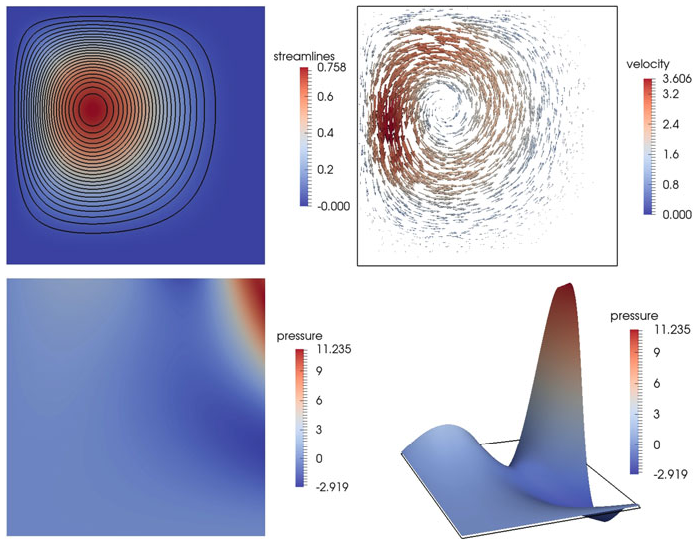
\includegraphics[width=\linewidth]{figures/Appendix_D/Fig_D_01__PDFp758__Bookp753.pdf}
 \captionof{figure}{例题 D.3:流函数(左上)、速度(右上)和压力(下);这些图由数值模拟结果绘制.}\label{fig:appendix-d-1}
\end{elegantfigure}
\end{example}

\begin{example}[二维驱动方腔问题]\label{ex:appendix-d-4}
二维驱动方腔问题是二维稳态流动中最常用的测试算例.区域为 $\Omega=(0,1)^2$,体力为零,即 Navier--Stokes 方程\hyperref[eq:steady-ns-strong]{(6.1)}中的右端项 $\bm f=0$.经典驱动方腔问题的边界条件通常写为
\begin{equation}\label{eq:appendix-d-10}
\bm u=\begin{pmatrix}0\\0\end{pmatrix}
\quad\text{当 }x=0,\ x=1\text{ 或 }y=0,\qquad
\bm u=\begin{pmatrix}1\\0\end{pmatrix}
\quad\text{当 }y=1.
\end{equation}
各算例由雷诺数 $\mathrm{Re}=\nu^{-1}$ 确定.

边界条件\hyperref[eq:appendix-d-10]{(D.10)}在方腔上角处有跳跃.若采用 Taylor--Hood 等有限元空间对,就必须指定速度在两个角点处的值.只有部分文献明确给出这种取值,例如\textcite{Olshanskii2002} 取
$\bm u(0,1)=\bm u(1,1)=(1,0)^\mathsf T$.无论角点处具体取何值,Dirichlet 边界数据都不属于 $H^{1/2}(\partial\Omega)$;由 $s=1$ 时的迹定理\hyperref[thm:appendix-a-34]{A.34},速度不可能属于 $H^1(\Omega)$.因此,经典驱动方腔问题不符合第\hyperref[chap:steady-navier-stokes]{6}章的理论框架.严格地说,该解的正则性不足以使用协调有限元方法.

经典驱动方腔问题的参考解通常取自\textcite{Ghia1982},其中给出了
$\mathrm{Re}\in\{100,400,1000,3200,5000,7500,10000\}$ 时的流线、截线上的解剖面和涡旋中心位置.然而,\textcite{Cazemier1998}、\textcite{Tiesinga2002}、\textcite{BruneauSaad2006} 等研究表明,经典顶盖驱动方腔的稳态解在 $\mathrm{Re}\approx8000$ 时失稳;当 $\mathrm{Re}=10000$ 时存在稳定的周期解.因此,若数值方法在 $\mathrm{Re}=10000$ 时得到稳定稳态解,就必须引入额外数值黏性.事实上,\textcite{Ghia1982} 使用有限差分格式,并采用了某种迎风型稳定化.

为消除上角点处的奇异性,文献提出了正则化驱动方腔问题,例如见\textcite[第 125 页]{Elman2014}.定义此类问题时,必须确保边界上也满足 $\nabla\cdot\bm u=0$,且角点处的散度完全由给定边界条件确定.\textcite{deFrutos2016c} 提出的一种满足这些要求的正则化问题采用如下边界条件:
\begin{equation}\label{eq:appendix-d-11}
\begin{aligned}
\bm u(x,1)&=\begin{pmatrix}u_1(x)\\0\end{pmatrix},\\
u_1(x)&=\begin{cases}
1-\tfrac14\bigl(1-\cos(\pi(x_1-x)/x_1)\bigr)^2,&x\in[0,x_1],\\[1mm]
1,&x\in(x_1,1-x_1),\\[1mm]
1-\tfrac14\bigl(1-\cos(\pi(x-(1-x_1))/x_1)\bigr)^2,&x\in[1-x_1,1].
\end{cases}
\end{aligned}
\end{equation}
本书所示模拟均取 $x_1=0.1$.图\hyperref[fig:appendix-d-2]{D.2}展示了
$\mathrm{Re}=1$ 和 $\mathrm{Re}=3200$ 时的解.低雷诺数时有一个靠近上边界的大涡旋,压力在两个上角处均出现较高峰值.$\mathrm{Re}=3200$ 时,速度场包含一个位于方腔中心附近的大涡旋、两个下角处的反向小涡旋,以及左边界上部的一个反向小涡旋;压力在右上角达到正峰值.
\begin{elegantfigure}[0.94\linewidth]
 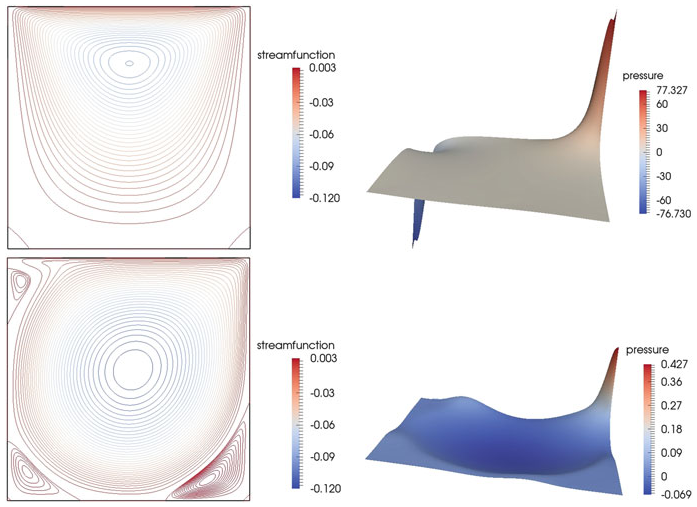
\includegraphics[width=\linewidth]{figures/Appendix_D/Fig_D_02__PDFp760__Bookp755.pdf}
 \captionof{figure}{例题 D.4:满足边界条件\hyperref[eq:appendix-d-11]{(D.11)}的正则化驱动方腔问题.$\mathrm{Re}=1$(上)和 $\mathrm{Re}=3200$(下)的流函数与压力.}\label{fig:appendix-d-2}
\end{elegantfigure}
\end{example}

\begin{example}[二维中 $\mathrm{Re}=20$ 的定常圆柱绕流]\label{ex:appendix-d-5}
该算例由\textcite{SchaeferTurek1996}提出,考虑二维区域中的圆形圆柱绕流,区域示意见图\hyperref[fig:appendix-d-3]{D.3}.
\begin{elegantfigure}[0.75\linewidth]
 
\includegraphics[page=760,pagebox=cropbox,trim=79.50bp 248.65bp 79.61bp 351.00bp,clip,width=\linewidth]{../input/source/Finite Element Methods for Incompressible Flow Problems.pdf}
 \captionof{figure}{例题 D.5:计算区域.}\label{fig:appendix-d-3}
\end{elegantfigure}
流体的动力黏度为 $\mu=10^{-3}\,\mathrm{Pa\,s}$,密度为 $\rho=1\,\mathrm{kg/m^3}$,其数值近似对应水.入口采用抛物线速度剖面
\begin{equation}\label{eq:appendix-d-12}
\bm v(0\,\mathrm m,y)
=\frac{1}{0.41^2}
\begin{pmatrix}1.2y(0.41-y)\\0\end{pmatrix}
\frac{\mathrm m}{\mathrm s},
\qquad 0\,\mathrm m\le y\le0.41\,\mathrm m.
\end{equation}
通道上、下壁面以及圆柱表面均施加无滑移条件.出口有两种可选边界条件:抛物线速度
\[
\bm v(2.2\,\mathrm m,y)
=\frac{1}{0.41^2}
\begin{pmatrix}1.2y(0.41-y)\\0\end{pmatrix}
\frac{\mathrm m}{\mathrm s},
\qquad 0\,\mathrm m\le y\le0.41\,\mathrm m,
\]
或 do-nothing 条件
\begin{equation}\label{eq:appendix-d-13}
\bm S\bm n=(\mu\nabla\bm v-P I)\bm n
=\bm 0\,\mathrm{N/m^2}
\qquad\text{于 }\Gamma_{\mathrm{out}},
\end{equation}
其中 $\bm n$ 为指向外侧的单位法向量.入口平均速度为
\[
U_{\mathrm{mean}}
=\frac{1}{0.41^2}
\frac{\int_0^{0.41}1.2y(0.41-y)\,\mathrm dy}
     {\int_0^{0.41}\mathrm dy}\,\frac{\mathrm m}{\mathrm s}
=0.2\,\mathrm{m/s}.
\]
以入口平均速度、圆柱直径 $d=0.1\,\mathrm m$ 及运动黏度 $\mu/\rho$ 为尺度,该流动的 Reynolds 数为 $\mathrm{Re}=20$.外力为零,即 $\bm f^{\mathrm{ext}}=\bm0\,\mathrm{N/m^3}$.此设置存在稳定稳态解,流场见图\hyperref[fig:appendix-d-4]{D.4}和\hyperref[fig:appendix-d-5]{D.5}.
\begin{elegantfigure}[0.84\linewidth]
 
\includegraphics[page=761,pagebox=cropbox,trim=52.50bp 112.15bp 52.36bp 437.00bp,clip,width=\linewidth]{../input/source/Finite Element Methods for Incompressible Flow Problems.pdf}
 \captionof{figure}{例题 D.5:圆柱绕流中的速度模(上)和压力(下).}\label{fig:appendix-d-4}
\end{elegantfigure}
\begin{elegantfigure}[0.84\linewidth]
 
\includegraphics[page=762,pagebox=cropbox,trim=52.50bp 488.90bp 52.36bp 60.25bp,clip,width=\linewidth]{../input/source/Finite Element Methods for Incompressible Flow Problems.pdf}
 \captionof{figure}{例题 D.5:圆柱表面附近的速度和压力.}\label{fig:appendix-d-5}
\end{elegantfigure}

取特征长度 $L=1\,\mathrm m$、特征速度 $U=1\,\mathrm{m/s}$,可得无量纲稳态 Navier--Stokes 方程\hyperref[eq:steady-ns-strong]{(6.1)}中的黏度 $\nu=\mu/(\rho UL)=10^{-3}$,入口条件
\[
\bm u(0,y)=\frac{1}{0.41^2}
\begin{pmatrix}1.2y(0.41-y)\\0\end{pmatrix},
\qquad 0\le y\le0.41,
\]
以及出口条件
\begin{equation}\label{eq:appendix-d-14}
\bm u(2.2,y)=\frac{1}{0.41^2}
\begin{pmatrix}1.2y(0.41-y)\\0\end{pmatrix},
\qquad 0\le y\le0.41,
\end{equation}
或
\begin{equation}\label{eq:appendix-d-15}
(\nu\nabla\bm u-pI)\bm n=\bm0
\qquad\text{于 }\Gamma_{\mathrm{out}}.
\end{equation}

感兴趣的量是物体所受的力,具体而言是阻力系数\hyperref[eq:appendix-d-3]{(D.3)}和升力系数\hyperref[eq:appendix-d-6]{(D.6)}.本二维算例中,主流方向为 $\bm w_{\mathrm{drag}}=(1,0)^\mathsf T$,与之正交的方向为 $\bm w_{\mathrm{lift}}=(0,1)^\mathsf T$;相对速度取 $V=U_{\mathrm{mean}}$,参考面积取圆柱直径 $A=d$.

笔记\hyperref[note:appendix-d-2]{D.2}介绍了计算阻力和升力系数的两种方法.由于圆柱是圆形,有限元网格无法精确表示其边界,若使用边界积分公式\hyperref[eq:appendix-d-4]{(D.4)}和\hyperref[eq:appendix-d-7]{(D.7)},仅边界近似就可能带来显著误差.因此应优先使用面积积分公式\hyperref[eq:appendix-d-5]{(D.5)}和\hyperref[eq:appendix-d-8]{(D.8)}.该算例为稳态问题且 $\bm f=0$,故对任意满足
$\bm w_{\mathrm{drag}}\in H^1(\Omega)^2$、在 $\partial\Omega\setminus\Gamma_{\mathrm{body}}$ 上为零且在 $\Gamma_{\mathrm{body}}$ 上取值 $(1,0)^\mathsf T$ 的函数,有
\begin{equation}\label{eq:appendix-d-16}
c_{\mathrm{drag}}
=-500\left[
(\nu\nabla\bm u,\nabla\bm w_{\mathrm{drag}})
+n(\bm u,\bm u,\bm w_{\mathrm{drag}})
-(\nabla\cdot\bm w_{\mathrm{drag}},p)
\right].
\end{equation}
这里采用稳态模拟中常见的黏性项形式,而 $n(\bm u,\bm u,\bm w_{\mathrm{drag}})$ 可取第\hyperref[subsec:steady-ns-nonlinear-term]{6.1.2}节介绍的任一种对流项形式.类似地,对任意在 $\partial\Omega\setminus\Gamma_{\mathrm{body}}$ 上为零、且在 $\Gamma_{\mathrm{body}}$ 上等于 $(0,1)^\mathsf T$ 的 $\bm w_{\mathrm{lift}}\in H^1(\Omega)^2$,有
\begin{equation}\label{eq:appendix-d-17}
c_{\mathrm{lift}}
=-500\left[
(\nu\nabla\bm u,\nabla\bm w_{\mathrm{lift}})
+n(\bm u,\bm u,\bm w_{\mathrm{lift}})
-(\nabla\cdot\bm w_{\mathrm{lift}},p)
\right].
\end{equation}

另一个感兴趣的量是圆柱前后两点间的压力差
\[
\Delta P=P(0.15,0.2)-P(0.25,0.2),
\]
其无量纲形式为
\begin{equation}\label{eq:appendix-d-18}
\Delta P=\rho U^2\bigl(p(0.15,0.2)-p(0.25,0.2)\bigr).
\end{equation}
当出口采用 Dirichlet 条件\hyperref[eq:appendix-d-14]{(D.14)}时,\textcite{JohnMatthies2001} 给出了相当准确的参考值:
\begin{equation}\label{eq:appendix-d-19}
c_{\mathrm{drag,ref}}=5.57953523384.
\end{equation}
\begin{equation}\label{eq:appendix-d-20}
c_{\mathrm{lift,ref}}=0.010618937712.
\end{equation}
\begin{equation}\label{eq:appendix-d-21}
\Delta p_{\mathrm{ref}}=0.11752016697.
\end{equation}
若出口采用 do-nothing 条件\hyperref[eq:appendix-d-15]{(D.15)},阻力系数和压力差参考值不变,升力系数则对出口条件稍敏感.\textcite{Nabh1998} 给出的升力系数参考值为
\begin{equation}\label{eq:appendix-d-22}
c_{\mathrm{lift,ref}}=0.010618948146.
\end{equation}
\end{example}

\begin{example}[三维中 $\mathrm{Re}=20$ 的定常圆柱绕流]\label{ex:appendix-d-6}
该问题是例题\hyperref[ex:appendix-d-5]{D.5} 的三维扩展,也由\textcite{SchaeferTurek1996}提出.区域为图\hyperref[fig:appendix-d-6]{D.6}所示、带圆柱的通道.通道高度为 $H=0.41\,\mathrm m$,圆柱直径为 $d=0.1\,\mathrm m$.没有外力,动量方程右端为 $\bm f=0$.流体的动力黏度为 $\mu=10^{-3}\,\mathrm{Pa\,s}$,密度为 $\rho=1\,\mathrm{kg/m^3}$.入口条件为
\[
\bm v|_{\mathrm{in}}
=\frac{1}{H^4}
\begin{pmatrix}
16Uyz(H-y)(H-z)\\0\\0
\end{pmatrix}\mathrm{m/s},
\qquad U=0.45\,\mathrm{m/s}.
\]
入口平均速度为
\[
U_{\mathrm{mean}}
=\frac{\int_0^H\int_0^H v_{\mathrm{in},1}\,\mathrm dy\,\mathrm dz}
        {\int_0^H\int_0^H\mathrm dy\,\mathrm dz}
=\frac{16\cdot0.45}{36}=0.2\,\mathrm{m/s}.
\]
因此,以 $U_{\mathrm{mean}}$、圆柱直径 $d$ 及运动黏度 $\mu/\rho$ 为尺度,该流动的 Reynolds 数为 $\mathrm{Re}=20$.
\begin{elegantfigure}[0.92\linewidth]
 
\includegraphics[page=764,pagebox=cropbox,trim=79.00bp 394.15bp 79.86bp 60.25bp,clip,width=\linewidth]{../input/source/Finite Element Methods for Incompressible Flow Problems.pdf}
 \captionof{figure}{例题 D.6:三维圆柱绕流计算区域.}\label{fig:appendix-d-6}
\end{elegantfigure}
取 $L=1\,\mathrm m$ 和 $U=1\,\mathrm{m/s}$,得到无量纲稳态 Navier--Stokes 方程\hyperref[eq:steady-ns-strong]{(6.1)},其中 $\nu=\mu/(\rho UL)=10^{-3}$.出口可采用与入口相同的速度条件,也可采用某种 do-nothing 条件;其余边界均施加无滑移条件 $\bm u=0$.与二维情形(例题\hyperref[ex:appendix-d-5]{D.5})一样,圆柱后方形成反向旋转的涡旋.若考察剖面,例如 $z=0.41/2$,流场形态与图\hyperref[fig:appendix-d-4]{D.4}和\hyperref[fig:appendix-d-5]{D.5}类似.

感兴趣的量为圆柱受到的阻力系数、升力系数及压力差
\begin{equation}\label{eq:appendix-d-23}
\Delta p=p(0.45,0.2,0.205)-p(0.55,0.2,0.205).
\end{equation}
阻力和升力系数的计算见笔记\hyperref[note:appendix-d-2]{D.2}.有限元方法需近似圆柱边界,因此应优先使用体积分.不过,此处物体与区域其余边界相连,故 $\bm w_{\mathrm{drag}}$ 和 $\bm w_{\mathrm{lift}}$ 的定义必须作折衷.例如,\textcite{John2002} 将 $\bm w_{\mathrm{drag}}$ 定义为与速度有限元多项式次数相同的有限元函数.圆柱边界上所有自由度——包括圆柱与区域左右边界交接处的自由度——都赋值为 $(1,0,0)^\mathsf T$;其余自由度赋值为零.$\bm w_{\mathrm{lift}}$ 采用相同构造,只是圆柱边界自由度取 $(0,1,0)^\mathsf T$.随后在\hyperref[eq:appendix-d-5]{(D.5)}和\hyperref[eq:appendix-d-8]{(D.8)}中取 $A=dH=0.041\,\mathrm{m^2}$、$V=U_{\mathrm{mean}}$,得到
\[
\begin{aligned}
c_{\mathrm{drag}}
&=-\frac{500}{0.41}\left[
(\nu\nabla\bm u,\nabla\bm w_{\mathrm{drag}})
+n(\bm u,\bm u,\bm w_{\mathrm{drag}})
-(\nabla\cdot\bm w_{\mathrm{drag}},p)\right],\\
c_{\mathrm{lift}}
&=-\frac{500}{0.41}\left[
(\nu\nabla\bm u,\nabla\bm w_{\mathrm{lift}})
+n(\bm u,\bm u,\bm w_{\mathrm{lift}})
-(\nabla\cdot\bm w_{\mathrm{lift}},p)\right].
\end{aligned}
\]
使用 Gaussian 等求积公式在单元内部计算系数时,$\bm w_{\mathrm{drag}}$ 和 $\bm w_{\mathrm{lift}}$ 的修改不会直接进入数值积分(求积点不会落在网格单元边界上),因此这种修改影响甚微.表\hyperref[tab:appendix-d-1]{D.1}列出了\textcite{SchaeferTurek1996} 给出的参考区间和\textcite{John2002} 给出的参考值.
\begin{eleganttable}
\captionof{table}{例题 D.6 的阻力系数、升力系数和压力差参考值.}\label{tab:appendix-d-1}
\begin{tabular}{lcc}
\toprule
量 & Schäfer 和 Turek(1996) & John(2002)\\
\midrule
$c_{\mathrm{drag}}$ & $[6.05,6.25]$ & $6.1853329$\\
$c_{\mathrm{lift}}$ & $[0.008,0.01]$ & $0.0094009839$\\
$\Delta p$ & $[0.165,0.175]$ & $0.1708$\\
\bottomrule
\end{tabular}
\end{eleganttable}
\end{example}

\section{层流非定常流动算例}\label{sec:appendix-d-2}

\begin{example}[单位正方形上给定解、齐次 Dirichlet 边界条件的非定常算例]\label{ex:appendix-d-7}
考虑 $\Omega=(0,1)^2$,取以下给定解:
\begin{equation}\label{eq:appendix-d-24}
\begin{aligned}
\bm u&=2\pi\sin(t)
\begin{pmatrix}
\sin^2(\pi x)\sin(\pi y)\cos(\pi y)\\
-\sin(\pi x)\cos(\pi x)\sin^2(\pi y)
\end{pmatrix},\\
p&=20\sin(t)\left(x^2y-\frac16\right).
\end{aligned}
\end{equation}
时刻 $t=1.7$ 的解见图\hyperref[fig:appendix-d-7]{D.7}.按定义,$\bm u|_{\partial\Omega}=0$.给定黏度后,选取右端项 $\bm f$,使式\hyperref[eq:appendix-d-24]{(D.24)}满足 Navier--Stokes 方程\hyperref[eq:dimensionless-ns-standard]{(2.25)}.
\begin{elegantfigure}[0.88\linewidth]
 
\includegraphics[page=766,pagebox=cropbox,trim=52.50bp 464.90bp 52.36bp 60.25bp,clip,width=\linewidth]{../input/source/Finite Element Methods for Incompressible Flow Problems.pdf}
 \captionof{figure}{例题 D.7:$t=1.7$ 时计算得到的解.}\label{fig:appendix-d-7}
\end{elegantfigure}
该测试问题可用于支持误差估计.为了覆盖式\hyperref[eq:appendix-d-24]{(D.24)}中的时间增长和衰减阶段,终止时间应足够长,例如\textcite{deFrutos2016c} 所取的 $T=5$.
\end{example}

\begin{example}[定常入口下 $\mathrm{Re}=100$ 的非定常圆柱绕流]\label{ex:appendix-d-8}
该算例描述层流 Kármán 涡街.其设置与例题\hyperref[ex:appendix-d-5]{D.5} 非常相似:计算区域、黏度、圆柱及通道上下壁面的边界条件、出口的 do-nothing 条件\hyperref[eq:appendix-d-13]{(D.13)}以及体力 $\bm f=0$ 均相同.唯一变化是入口速度增至式\hyperref[eq:appendix-d-12]{(D.12)}的五倍:
\begin{equation}\label{eq:appendix-d-25}
\bm v(0\,\mathrm m,y)
=\frac{1}{0.41^2}
\begin{pmatrix}6y(0.41-y)\\0\end{pmatrix}
\frac{\mathrm m}{\mathrm s},
\qquad 0\,\mathrm m\le y\le0.41\,\mathrm m.
\end{equation}
因此,与例题\hyperref[ex:appendix-d-5]{D.5}相比,特征速度尺度和 Reynolds 数也增大五倍,分别为 $U_{\mathrm{mean}}=1\,\mathrm{m/s}$ 和 $\mathrm{Re}=100$.此时问题不存在稳定稳态解,故应以非定常不可压缩 Navier--Stokes 方程\hyperref[eq:time-dependent-ns-strong]{(7.1)}为模型.采用与例题\hyperref[ex:appendix-d-5]{D.5}相同的特征尺度,无量纲黏度为 $\nu=10^{-3}$.

此问题需要初始条件,但不存在解析形式的初始解.可先用任意初始条件启动模拟,继续计算直至 Kármán 涡街形成并趋于周期状态.达到这一状态后,保存某一离散时刻的数值解,并将其作为后续模拟的初始条件.

与例题\hyperref[ex:appendix-d-5]{D.5}类似,感兴趣的量是圆柱所受阻力系数、升力系数,以及圆柱前后压力差.与稳态问题不同,动量方程还含速度的时间导数.由式\hyperref[eq:appendix-d-5]{(D.5)}和\hyperref[eq:appendix-d-8]{(D.8)}可得
\begin{equation}\label{eq:appendix-d-26}
\begin{aligned}
c_{\mathrm{drag}}=-20\Bigl[&(\partial_t\bm u,\bm w_{\mathrm{drag}})
+(\nu\nabla\bm u,\nabla\bm w_{\mathrm{drag}})\\
&+n(\bm u,\bm u,\bm w_{\mathrm{drag}})
-(\nabla\cdot\bm w_{\mathrm{drag}},p)\Bigr].
\end{aligned}
\end{equation}
\begin{equation}\label{eq:appendix-d-27}
\begin{aligned}
c_{\mathrm{lift}}=-20\Bigl[&(\partial_t\bm u,\bm w_{\mathrm{lift}})
+(\nu\nabla\bm u,\nabla\bm w_{\mathrm{lift}})\\
&+n(\bm u,\bm u,\bm w_{\mathrm{lift}})
-(\nabla\cdot\bm w_{\mathrm{lift}},p)\Bigr].
\end{aligned}
\end{equation}
其中 $\bm w_{\mathrm{drag}}$ 和 $\bm w_{\mathrm{lift}}$ 的定义见例题\hyperref[ex:appendix-d-5]{D.5}.时间导数项可用后向差分近似,例如
\[
(\partial_t\bm u,\bm w_{\mathrm{drag}})
\approx \frac{1}{\Delta t_{n+1}}
(\bm u^{n+1}-\bm u^n,\bm w_{\mathrm{drag}}).
\]
压力降按式\hyperref[eq:appendix-d-18]{(D.18)}计算.图\hyperref[fig:appendix-d-8]{D.8}给出了阻力系数、升力系数和压力降的典型变化.
\begin{elegantfigure}[0.92\linewidth]
 
\includegraphics[page=767,pagebox=cropbox,trim=53.00bp 86.40bp 53.11bp 308.75bp,clip,width=\linewidth]{../input/source/Finite Element Methods for Incompressible Flow Problems.pdf}
 \captionof{figure}{例题 D.8:感兴趣的量随时间的变化.}\label{fig:appendix-d-8}
\end{elegantfigure}

另一个感兴趣的泛函是 Strouhal 数\hyperref[eq:dimensionless-parameters]{(2.23)},它与周期长度密切相关(式\hyperref[eq:dimensionless-parameters]{(2.23)}中的 $T^*$ 表示周期长度).实际中,可以由阻力系数或升力系数的极值位置,或由升力系数的零点,估计周期长度.模拟一段时间后,对连续若干周期的长度取平均.
表\hyperref[tab:appendix-d-2]{D.2}列出\textcite{SchaeferTurek1996} 给出的感兴趣量参考区间.这里 $t_{0,\mathrm{per}}$ 是某一周期的起始时刻(升力系数达到极大值时),$T_{\mathrm{per}}$ 为周期长度.
\begin{eleganttable}
\captionof{table}{例题 D.8 的参考区间.}\label{tab:appendix-d-2}
\begin{tabular}{lc}
\toprule
量 & 参考区间\\
\midrule
$c_{\mathrm{drag,max}}$ & $[3.22,3.24]$\\
$c_{\mathrm{lift,max}}$ & $[0.98,1.02]$\\
$\Delta p(t_{0,\mathrm{per}}+T_{\mathrm{per}}/2)$ & $[2.46,2.50]$\\
Strouhal 数 & $[0.295,0.305]$\\
\bottomrule
\end{tabular}
\par\smallskip
\parbox{0.9\linewidth}{\centering 参考区间据\textcite{SchaeferTurek1996}.}
\end{eleganttable}
\end{example}

\begin{example}[时变入口下 Reynolds 数介于 $0$ 与 $100$ 的非定常圆柱绕流]\label{ex:appendix-d-9}
该算例描述涡脱落的产生和衰减,其设置与例题\hyperref[ex:appendix-d-5]{D.5}几乎相同,只有入口边界条件不同:
\begin{equation}\label{eq:appendix-d-28}
\begin{aligned}
\bm v(t',0,y)
&=\sin\left(\frac{\pi t'}{8\,\mathrm s}\right)
\frac{1}{0.41^2}
\begin{pmatrix}6y(0.41-y)\\0\end{pmatrix}
\frac{\mathrm m}{\mathrm s},\\
&\qquad y\in[0,0.41]\,\mathrm m,\quad t'\in[0,8]\,\mathrm s.
\end{aligned}
\end{equation}
其频率为 $\Omega=\pi\,\mathrm{s}^{-1}$.该算例的入口平均速度为
\[
U_{\mathrm{mean}}(t')
=\sin\left(\frac{\pi t'}{8\,\mathrm s}\right)
\frac{\int_0^{0.41}6y(0.41-y)\,\mathrm dy}
     {0.41^2\int_0^{0.41}\mathrm dy}
\frac{\mathrm m}{\mathrm s}
=\sin\left(\frac{\pi t'}{8\,\mathrm s}\right)\frac{\mathrm m}{\mathrm s}.
\]
以圆柱直径 $d=0.1\,\mathrm m$、入口平均速度及运动黏度 $\mu/\rho$ 为尺度,该流动的 Reynolds 数满足 $0\le\mathrm{Re}(t')\le100$.出口可采用与式\hyperref[eq:appendix-d-28]{(D.28)}相应的 Dirichlet 条件
\begin{equation}\label{eq:appendix-d-29}
\begin{aligned}
\bm v(t',2.2\,\mathrm m,y)
&=\sin\left(\frac{\pi t'}{8\,\mathrm s}\right)
\frac{1}{0.41^2}
\begin{pmatrix}6y(0.41-y)\\0\end{pmatrix}
\frac{\mathrm m}{\mathrm s},\\
&\qquad y\in[0,0.41]\,\mathrm m,\quad t'\in[0,8]\,\mathrm s.
\end{aligned}
\end{equation}
也可采用 do-nothing 条件
\begin{equation}\label{eq:appendix-d-30}
\bm S(t')\bm n
=\bigl(2\mu D(\bm v)(t')-P(t')I\bigr)\bm n
=\bm0\,\mathrm{N/m^2}
\quad\text{于 }\Gamma_{\mathrm{out}},\quad t'\in[0,8]\,\mathrm s.
\end{equation}
初始条件取 $\bm v_0=0\,\mathrm{m/s}$.图\hyperref[fig:appendix-d-9]{D.9}展示了不同时刻的流场.
\begin{elegantfigure}[0.92\linewidth]
 
\includegraphics[page=769,pagebox=cropbox,trim=52.50bp 236.90bp 52.36bp 60.25bp,clip,width=\linewidth]{../input/source/Finite Element Methods for Incompressible Flow Problems.pdf}
 \captionof{figure}{例题 D.9:速度场的时间演化,分别显示 $2$、$4$、$5$、$6$、$7$ 和 $8$ 秒时的结果.}\label{fig:appendix-d-9}
\end{elegantfigure}

无量纲入口条件为
\[
\begin{aligned}
\bm u(0,y)
&=\sin\left(\frac{\pi t}{8}\right)
\frac{1}{0.41^2}
\begin{pmatrix}6y(0.41-y)\\0\end{pmatrix},\\
&\qquad 0\le y\le0.41,\quad t\in[0,8].
\end{aligned}
\]
与例题\hyperref[ex:appendix-d-5]{D.5}一样,感兴趣的量为阻力系数\hyperref[eq:appendix-d-3]{(D.3)}、升力系数\hyperref[eq:appendix-d-6]{(D.6)}及圆柱前后压力差
\[
\Delta P(t)=P(t,0.15,0.2)-P(t,0.25,0.2).
\]
由于有限元三角剖分无法精确表示圆周边界,阻力和升力应采用面积积分公式\hyperref[eq:appendix-d-5]{(D.5)}和\hyperref[eq:appendix-d-8]{(D.8)},而不是边界积分公式\hyperref[eq:appendix-d-4]{(D.4)}和\hyperref[eq:appendix-d-7]{(D.7)}.这些公式中取 $U=1\,\mathrm{m/s}$、$L=1\,\mathrm m$、$A=0.1\,\mathrm m$、$V=U_{\mathrm{mean}}(4\,\mathrm s)=1\,\mathrm{m/s}$,便得到式\hyperref[eq:appendix-d-26]{(D.26)}和\hyperref[eq:appendix-d-27]{(D.27)}.

\textcite{JohnRang2010} 对感兴趣的量计算了精确度较高的参考曲线,见图\hyperref[fig:appendix-d-10]{D.10}.这些曲线对应出口采用 Dirichlet 条件\hyperref[eq:appendix-d-29]{(D.29)}的情形.表\hyperref[tab:appendix-d-3]{D.3}列出参考值.
\begin{elegantfigure}[0.92\linewidth]
 
\includegraphics[page=770,pagebox=cropbox,trim=52.50bp 168.90bp 53.61bp 225.50bp,clip,width=\linewidth]{../input/source/Finite Element Methods for Incompressible Flow Problems.pdf}
 \captionof{figure}{例题 D.9:据\textcite{JohnRang2010}给出的感兴趣量参考曲线.}\label{fig:appendix-d-10}
\end{elegantfigure}
\begin{eleganttable}
\captionof{table}{例题 D.9 的参考值.}\label{tab:appendix-d-3}
\begin{tabular}{lcc}
\toprule
量 & 数值 & 时刻\\
\midrule
$c_{\mathrm{drag,max}}^{\mathrm{ref}}$ & $2.950918381$ & $3.93625$\\
$c_{\mathrm{lift,max}}^{\mathrm{ref}}$ & $0.47787543$ & $5.69250$\\
$\Delta p(8\,\mathrm s)^{\mathrm{ref}}$ & $-0.11161567$ & \\
\bottomrule
\end{tabular}
\par\smallskip
\parbox{0.9\linewidth}{\centering 参考值据\textcite{JohnRang2010}.}
\end{eleganttable}
\end{example}

\begin{example}[二维和三维指数衰减流动:Beltrami 流]\label{ex:appendix-d-10}
设 $\Omega\subset\mathbb R^3$,考虑以下速度场和压力场族:
\begin{equation}\label{eq:appendix-d-31}
\bm u=-\alpha e^{-\nu\gamma^2t}
\begin{pmatrix}
e^{\alpha x}\sin(\alpha y+\gamma z)+e^{\alpha z}\cos(\alpha x+\gamma y)\\
e^{\alpha y}\sin(\alpha z+\gamma x)+e^{\alpha x}\cos(\alpha y+\gamma z)\\
e^{\alpha z}\sin(\alpha x+\gamma y)+e^{\alpha y}\cos(\alpha z+\gamma x)
\end{pmatrix},
\end{equation}
\[
\begin{aligned}
p=-\frac{\alpha^2}{2}e^{-2\nu\gamma^2t}\bigl[&
e^{2\alpha x}+e^{2\alpha y}+e^{2\alpha z}\\
&+2\sin(\alpha x+\gamma y)\cos(\alpha z+\gamma x)e^{\alpha(y+z)}\\
&+2\sin(\alpha y+\gamma z)\cos(\alpha x+\gamma y)e^{\alpha(z+x)}\\
&+2\sin(\alpha z+\gamma x)\cos(\alpha y+\gamma z)e^{\alpha(x+y)}
\bigr]+C.
\end{aligned}
\]
这里 $\alpha,\gamma\in\mathbb R$ 是用户选取的参数,见图\hyperref[fig:appendix-d-11]{D.11}.若在 $\partial\Omega$ 上施加 Dirichlet 边界条件,则常数 $C$ 应选得使 $p$ 的积分平均值为零.将式\hyperref[eq:appendix-d-31]{(D.31)}代入 Navier--Stokes 方程\hyperref[eq:time-dependent-ns-strong]{(7.1)},直接计算可得 $\bm f=0$.这族解由\textcite{EthierSteinman1994} 推导,其构造依据以下原则:
\begin{itemize}
  \item 速度场应无散;
  \item 时间导数应与黏性项平衡,即 $\partial_t\bm u-\nu\Delta\bm u=0$;
  \item 对流项应能表示为某个标量函数的梯度,且该梯度与压力梯度互相抵消,即 $(\bm u\cdot\nabla)\bm u+\nabla p=0$.
\end{itemize}
直接计算可得
\begin{equation}\label{eq:appendix-d-32}
\nabla\times(\nabla\times\bm u)=0.
\end{equation}
满足性质\hyperref[eq:appendix-d-32]{(D.32)}的流称为 Beltrami 流.图\hyperref[fig:appendix-d-11]{D.11}展示了 $t=0$ 时 $\alpha=\pi/4$、$\gamma=\pi/2$ 的速度和压力.
\begin{elegantfigure}[0.92\linewidth]
 
\includegraphics[page=771,pagebox=cropbox,trim=52.50bp 116.40bp 52.36bp 411.50bp,clip,width=\linewidth]{../input/source/Finite Element Methods for Incompressible Flow Problems.pdf}
 \captionof{figure}{例题 D.10:区域 $\Omega=(-1,1)\times(-1,1)\times(0,2)$ 上 $t=0$ 时的速度和压力,参数取 $\alpha=\pi/4$、$\gamma=\pi/2$.}\label{fig:appendix-d-11}
\end{elegantfigure}

\textcite{Taylor1923} 早已提出二维区域 $\Omega=(0,\pi)^2$ 上的指数衰减流动问题:
\[
\bm u=e^{-2\nu t}
\begin{pmatrix}
-\cos x\sin y\\
\sin x\cos y
\end{pmatrix},
\qquad
p=-\frac14e^{-4\nu t}\bigl(\cos(2x)+\cos(2y)\bigr).
\]
例如,\textcite{Chorin1968} 对这类解进行了数值研究.
\end{example}

\begin{note}[时变入口下三维 $\mathrm{Re}\in[0,100]$ 圆柱绕流]\label{note:appendix-d-11}
\textcite{SchaeferTurek1996} 还定义了例题\hyperref[ex:appendix-d-9]{D.9} 的三维扩展,其设置与例题\hyperref[ex:appendix-d-6]{D.6} 相似.与后者相比,该问题的入口速度随时间变化,且在大部分时间区间内更强.然而,\textcite{John2006} 发现该算例不会发生涡脱落.由于缺少这一流动特征,采用此算例的意义有限.
\end{note}

\section{湍流算例}\label{sec:appendix-d-3}

\begin{example}[湍流槽道流]\label{ex:appendix-d-12}
湍流槽道流由如下无量纲不可压缩 Navier--Stokes 方程组描述,其中体力项为 $\bm f=(1,0,0)^\mathsf T$:
\begin{equation}\label{eq:appendix-d-33}
\begin{aligned}
\partial_t\bm u
-2\nabla\cdot\bigl(\mathrm{Re}_{\tau}^{-1}D(\bm u)\bigr)
+(\bm u\cdot\nabla)\bm u+\nabla p
&=\bm f
&&\text{于 }(0,T]\times\Omega,\\
\nabla\cdot\bm u&=0
&&\text{于 }(0,T]\times\Omega,
\end{aligned}
\end{equation}
方程组\hyperref[eq:appendix-d-33]{(D.33)}采用特征长度 $L=1\,\mathrm m$ 和特征速度 $U=1\,\mathrm{m/s}$ 导出.因此,无量纲黏度为 $\nu=\mathrm{Re}_{\tau}^{-1}$(见笔记\hyperref[note:characteristic-scales]{2.19}),流体的运动黏度为 $\mathrm{Re}_{\tau}^{-1}\,\mathrm{m^2/s}$.

文献中对若干 $\mathrm{Re}_\tau$ 给出了基准问题.

\paragraph{$\mathrm{Re}_\tau=180$ 的湍流槽道流.}
计算区域为
\[
\Omega=(-2\pi,2\pi)\times(0,2H)\times
\left(-\frac{2\pi}{3},\frac{2\pi}{3}\right),
\]
其中槽道半宽 $H=1$,$\mathrm{Re}_\tau=180$ 是以半宽、流体运动黏度和剪切速度(或摩擦速度)$U_\tau$ 定义的 Reynolds 数,见笔记\hyperref[note:turbulent-boundary-layers]{8.13}.由
$\mathrm{Re}_\tau=U_\tau H/\nu$,取 $\nu=\mathrm{Re}_\tau^{-1}\,\mathrm{m^2/s}$ 得
$U_\tau=1\,\mathrm{m/s}$,从而无量纲摩擦速度 $u_\tau=U_\tau/U=1$.流向 $x$ 和展向 $z$ 采用周期边界条件;固壁位于 $y=0$ 和 $y=2$,并施加无滑移条件 $\bm u=0$.

初始条件可依据\textcite{Moser1999} 所提供数据文件 \texttt{chan180.means} 中的已知平均速度剖面 $U_{\mathrm{mean}}(y)$ 构造,见图\hyperref[fig:appendix-d-12]{D.12}.对该平均速度剖面作线性插值,并加入随机扰动,例如采用\textcite{Gravemeier2006b} 提出的形式:
\begin{equation}\label{eq:appendix-d-34}
\begin{aligned}
u_1(0;x,y,z)&=U_{\mathrm{mean}}(y)+0.1U_{\mathrm{bulk}}\,\varepsilon(x,y,z),\\
u_2(0;x,y,z)&=0.1U_{\mathrm{bulk}}\,\varepsilon(x,y,z),\\
u_3(0;x,y,z)&=0.1U_{\mathrm{bulk}}\,\varepsilon(x,y,z),
\end{aligned}
\end{equation}
其中
\begin{equation}\label{eq:appendix-d-35}
U_{\mathrm{bulk}}=\frac1H\int_0^H U_{\mathrm{mean}}(y)\,\mathrm dy
\approx15.6803.
\end{equation}
为通过数值积分计算这一数值,$U_{\mathrm{mean}}(y)$ 以三次样条插值.随机函数 $\varepsilon$ 可按 C++ 记法取为
\[
\varepsilon(x,y,z)=\frac{2\,\mathrm{rand}()}{\mathrm{RAND\_MAX}}-1
\in[-1,1].
\]
总之,初始速度场\hyperref[eq:appendix-d-34]{(D.34)}是在插值所得平均速度剖面 $U_{\mathrm{mean}}(y)$ 上加入随机速度扰动,扰动幅度为整体平均速度 $U_{\mathrm{bulk}}$ 的 $20\%$(正、负方向各占 $10\%$).图\hyperref[fig:appendix-d-13]{D.13}给出了计算流场的一个瞬时快照.整体来看,流动方向由左至右.截面上的速度显示,槽道内部的平均流速高于靠近边界处的流速,这符合预期;但边界附近也有涡旋,因此局部流动也会朝反方向运动.
\begin{elegantfigure}[0.55\linewidth]
 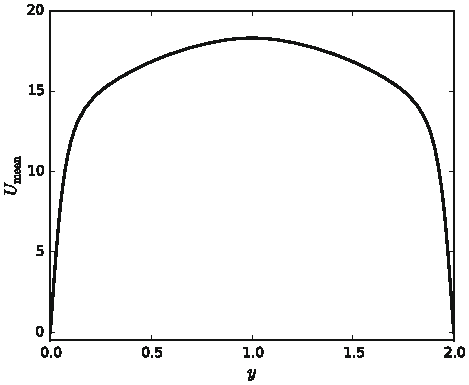
\includegraphics[width=\linewidth]{figures/Appendix_D/Fig_D_12__PDFp773__Bookp768.pdf}
 \captionof{figure}{例题 D.12:据数据文件 \texttt{chan180.means} 绘制的 $\mathrm{Re}_\tau=180$ 湍流槽道流平均速度剖面 $U_{\mathrm{mean}}(y)$.}\label{fig:appendix-d-12}
\end{elegantfigure}
\begin{elegantfigure}[0.94\linewidth]
 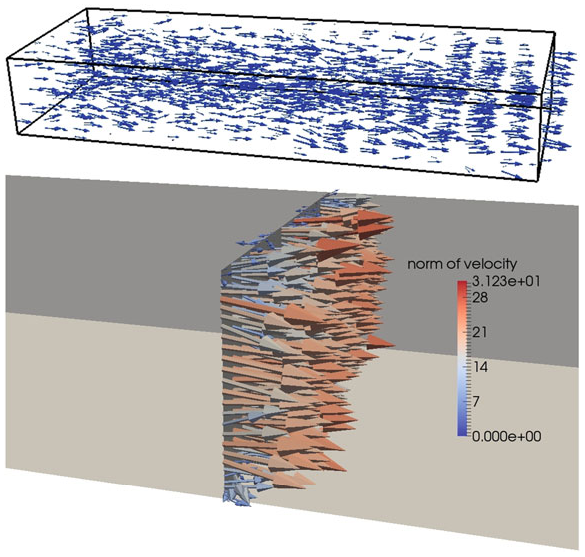
\includegraphics[width=\linewidth]{figures/Appendix_D/Fig_D_13__PDFp774__Bookp769.pdf}
 \captionof{figure}{例题 D.12:$\mathrm{Re}_\tau=180$ 湍流槽道流的速度场快照;上图为整个槽道,下图为垂直于 $x$ 方向的截面(浅灰平面 $y=0$,深灰平面 $z=2\pi/3$).}\label{fig:appendix-d-13}
\end{elegantfigure}

\paragraph{$\mathrm{Re}_\tau=395$ 的湍流槽道流.}
此问题的计算区域为
\[
\Omega=(-\pi,\pi)\times(0,2)\times
\left(-\frac{\pi}{2},\frac{\pi}{2}\right),
\]
固壁仍位于 $y=0$ 和 $y=2$,其余边界仍为周期边界.与 $\mathrm{Re}_\tau=180$ 的情形相同,有 $u_\tau=U_\tau/U=1$.采用\textcite{Moser1999} 的参考平均速度,得到整体平均速度 $U_{\mathrm{bulk}}=17.5452$.初始条件可按 $\mathrm{Re}_\tau=180$ 的方法构造.

\paragraph{感兴趣的统计量.}
用 $\langle\cdot\rangle_t$ 表示时间平均,用 $\langle\cdot\rangle_s$ 表示对空间均匀方向的平均.湍流槽道流的均匀方向是流向 $x$ 和展向 $z$.若时间步等距,有限元速度的时间平均可用算术平均计算:
\[
\langle\bm u^h(t,\bm x)\rangle_t
=\frac1{N_t+1}\sum_{n=0}^{N_t}\bm u^h(t_n,\bm x),
\]
其中 $N_t$ 为时间步数.同理,若均匀方向上的网格等距,空间平均也可用算术平均计算,例如
\[
\langle\bm u^h(t_n,x,y,z)\rangle_s
=\frac1{N_xN_z}\sum_{i=1}^{N_x}\sum_{j=1}^{N_z}
\bm u^h(t_n,x_i,y,z_j),
\]
其中 $N_x$、$N_z$ 分别为 $x$ 和 $z$ 方向的自由度数.

感兴趣的统计量包括平均速度和 Reynolds 应力.前者是一次平均量:
\[
\bm u^h_{\mathrm{mean}}(y)
=\left\langle\left\langle
\bm u^h(t,x,y,z)\right\rangle_s\right\rangle_t,
\]
后者为二次平均量
\begin{equation}\label{eq:appendix-d-36}
T^h_{ij,\mathrm{mean}}
=\left\langle\left\langle u_i^h u_j^h\right\rangle_s\right\rangle_t
-\left\langle\left\langle u_i^h\right\rangle_s\right\rangle_t
 \left\langle\left\langle u_j^h\right\rangle_s\right\rangle_t,
\qquad i,j=1,2,3.
\end{equation}
Reynolds 应力张量的定义见笔记\hyperref[note:les-closure-problem]{8.32}.平均速度中尤为关心第一分量 $u^h_{1,\mathrm{mean}}(y)$.

文献中对 Reynolds 应力的定义并不统一,\textcite{JohnRoland2007} 对此作了讨论.\textcite{Winckelmans2002} 指出,用湍流模拟解计算得到的对角 Reynolds 应力(即式\hyperref[eq:appendix-d-36]{(D.36)}中 $i=j$ 的情形),不能与真实湍流流场的对角应力直接比较.原因在于湍流模型用亚格子尺度应力张量的迹定义修正压力,而模拟中无法获得这一迹(参见亚格子尺度应力偏差部分\hyperref[eq:sgs-deviatoric-part]{(8.61)}).可直接研究的只有所谓 rms(均方根)湍流强度:
\begin{equation}\label{eq:appendix-d-37}
u^h_{i,\mathrm{rms}}
=\left|T^h_{ii,\mathrm{mean}}
-\frac13\sum_{j=1}^{3}T^h_{jj,\mathrm{mean}}\right|^{1/2},
\qquad i=1,2,3.
\end{equation}
\textcite{Winckelmans2002} 还指出,计算二阶统计量\hyperref[eq:appendix-d-36]{(D.36)}和 rms 量\hyperref[eq:appendix-d-37]{(D.37)}时,应计入所用湍流模型的贡献.对于某些模型,这一贡献易于识别和实现,例如式\hyperref[eq:smagorinsky-turbulent-viscosity]{(8.66)}中的 Smagorinsky 模型;另见\textcite{JohnRoland2007}.不过,有些湍流模型的贡献很难纳入.

\paragraph{离散化的若干方面.}
模拟中通常在 $x$、$z$ 方向使用均匀网格,在壁面法向 $y$ 方向使用分级网格,并在靠近壁面处加密;例如可参见\textcite{Gravemeier2006a,Gravemeier2006b} 给出的两种方案.等距时间步长应足够小,以分辨流动的时间变化.\textcite{ChoiMoin1994} 的研究建议满足
\begin{equation}\label{eq:appendix-d-38}
\Delta t^+=u_\tau\mathrm{Re}_\tau\Delta t\le0.4.
\end{equation}

\paragraph{有限元模拟中的一项注意事项.}
由于流动不可压缩,模拟过程中整体平均速度理应保持不变.然而,有限元函数一般并非弱无散,而只是离散无散.因此,有限元离散不会自动保证整体平均速度守恒(这对应质量守恒).\textcite{JohnRoland2007} 提出,可动态调整 Navier--Stokes 方程组的右端项,以校正计算得到的整体平均速度与式\hyperref[eq:appendix-d-35]{(D.35)}之差.流动由压力梯度驱动.设 $U_{\mathrm{bulk,sim}}(t_n)$ 是时刻 $t_n$ 的数值解整体平均速度,则在 $t_{n+1}$ 时刻,方程组\hyperref[eq:appendix-d-33]{(D.33)}的右端项取为
\begin{equation}\label{eq:appendix-d-39}
\bm f
=\begin{pmatrix}1\\0\\0\end{pmatrix}
+\frac{1}{\Delta t_n}
\begin{pmatrix}
U_{\mathrm{bulk}}-U_{\mathrm{bulk,sim}}(t_n)\\0\\0
\end{pmatrix}.
\end{equation}
这里 $\Delta t_n$ 为时间步长.对于具有物理量纲的量,式\hyperref[eq:appendix-d-39]{(D.39)}中的修正项具有正确的物理单位.因此,若 $U_{\mathrm{bulk,sim}}(t_n)<U_{\mathrm{bulk}}$,流动将被加速,数值解的整体平均速度随之增大;若 $U_{\mathrm{bulk,sim}}(t_n)>U_{\mathrm{bulk}}$,驱动力将小于 $1$,数值解的整体平均速度会在下一离散时刻减小.

\textcite{JohnRoland2007} 报告说,若不采用式\hyperref[eq:appendix-d-39]{(D.39)}所示的驱动力动态校正,数值解的整体平均速度可能增大,也可能减小,具体取决于湍流模型.采用这一校正后,整体平均速度仍有一定振荡,但始终接近式\hyperref[eq:appendix-d-35]{(D.35)}给出的值,通常误差小于 $1\%$.
\end{example}

\begin{example}[正方形截面柱绕流,$\mathrm{Re}=22000$]\label{ex:appendix-d-13}
该槽道绕障碍物流动算例由\textcite{Rodi1997}定义.障碍物实际上是立柱,但文献中通常称之为圆柱.图\hyperref[fig:appendix-d-14]{D.14}示意了流动区域的截面,通道高度为 $H=0.4\,\mathrm m$.入口速度为
\begin{equation}\label{eq:appendix-d-40}
\bm u(t,0,y,z)
=\begin{pmatrix}1+0.04\,\mathrm{rand}\\0\\0\end{pmatrix},
\qquad \mathrm{rand}\in[-0.5,0.5].
\end{equation}
入口噪声用于激发湍流.立柱表面施加无滑移条件;在 $x=2.5\,\mathrm m$ 处施加出口条件\hyperref[eq:do-nothing-condition]{(2.37)};其他边界施加自由滑移条件\hyperref[eq:free-slip-condition]{(2.34)}.由于初始条件未知,可先选取某个初始条件,例如将入口条件在初始时刻插值延拓到区域内部,继续模拟至流动充分发展后再计算感兴趣的统计量.该算例描述统计周期流动,图\hyperref[fig:appendix-d-15]{D.15}给出了一个瞬时快照.区域截面示意见图\hyperref[fig:appendix-d-14]{D.14}.
\begin{elegantfigure}[0.7\linewidth]
 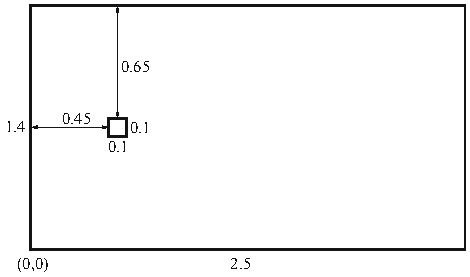
\includegraphics[width=\linewidth]{figures/Appendix_D/Fig_D_14__PDFp777__Bookp772.pdf}
 \captionof{figure}{例题 D.13:流动区域 $x$-$y$ 截面图(长度单位均为米),通道高度 $H=0.4\,\mathrm m$.}\label{fig:appendix-d-14}
\end{elegantfigure}
\begin{elegantfigure}[0.92\linewidth]
 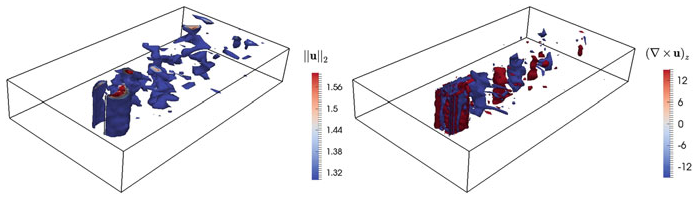
\includegraphics[width=\linewidth]{figures/Appendix_D/Fig_D_15__PDFp778__Bookp773.pdf}
 \captionof{figure}{例题 D.13:速度模等值面(左)和涡量第三分量(见式(3.151),右)的快照;可清楚看到立柱后方的涡脱落.}\label{fig:appendix-d-15}
\end{elegantfigure}

以入口平均速度 $U=1\,\mathrm{m/s}$、立柱边长 $D=0.1\,\mathrm m$ 及运动黏度 $\nu=1/220000\,\mathrm{m^2/s}$ 为尺度,得到 $\mathrm{Re}=UD/\nu=22000$.

与通常的绕体流动一样,感兴趣的量为阻力系数和升力系数.它们可用体积分计算,公式见\hyperref[eq:appendix-d-5]{(D.5)}和\hyperref[eq:appendix-d-8]{(D.8)}.此例取
\[
\begin{aligned}
L=1\,\mathrm m,\qquad V=U,\qquad A=DH,\\
\bm w_{\mathrm{drag}}=\begin{pmatrix}1\\0\\0\end{pmatrix},
\qquad
\bm w_{\mathrm{lift}}=\begin{pmatrix}0\\1\\0\end{pmatrix}.
\end{aligned}
\]
在立柱与自由滑移边界的连接处,$\bm w_{\mathrm{drag}}$ 和 $\bm w_{\mathrm{lift}}$ 应按例题\hyperref[ex:appendix-d-6]{D.6}所述方式设置.Strouhal 数定义为
\[
\mathrm{St}=\frac{DU}{T},
\]
其中 $T$ 为平均周期长度.感兴趣的量包括 Strouhal 数、时间平均阻力系数和升力系数 $\overline{c}_{\mathrm{drag}}$、$\overline{c}_{\mathrm{lift}}$,以及阻力和升力系数的均方根值.对 $n=1,\ldots,N_t$,定义阻力系数和升力系数相对于各自时间平均值的偏差:
\[
\begin{aligned}
\delta_{\mathrm{drag},n}&=c_{\mathrm{drag}}(t_n)-\overline c_{\mathrm{drag}},\\
\delta_{\mathrm{lift},n}&=c_{\mathrm{lift}}(t_n)-\overline c_{\mathrm{lift}}.
\end{aligned}
\]
相应的均方根值为
\[
\begin{aligned}
c_{\mathrm{drag,rms}}&=\left(\frac1{N_t}\sum_{n=1}^{N_t}\delta_{\mathrm{drag},n}^{\,2}\right)^{1/2},\\
c_{\mathrm{lift,rms}}&=\left(\frac1{N_t}\sum_{n=1}^{N_t}\delta_{\mathrm{lift},n}^{\,2}\right)^{1/2}.
\end{aligned}
\]
求和覆盖计算阻力和升力系数的整个时间区间内所有离散时刻.实验参考值见\textcite{Rodi1997}:
\[
\begin{aligned}
\overline c_{\mathrm{drag}}\in[1.9,2.1],\qquad
c_{\mathrm{drag,rms}}\in[0.1,0.2],\\
c_{\mathrm{lift,rms}}\in[0.7,1.4],\qquad
\mathrm{St}=0.132.
\end{aligned}
\]
由于涡脱落具有统计周期性,$\overline c_{\mathrm{lift}}=0$.
\end{example}

\begin{example}[$\mathrm{Re}=40000$ 的壁面立方体绕流]\label{ex:appendix-d-14}
在此算例中,流体不但绕过物体,也会越过物体流动.该问题见\textcite{Hoffman2005,HoffmanJohnson2006};\textcite{Rodi1997} 也提出过类似算例.$z=0$ 处区域底面的示意见图\hyperref[fig:appendix-d-16]{D.16}.立方体高度为 $H$,通道高度为 $2H$.\textcite{Hoffman2005,HoffmanJohnson2006} 的模拟取 $H=0.1\,\mathrm m$.

此算例中没有体力,即 $\bm f=0$.表\hyperref[tab:appendix-d-4]{D.4}给出了平均流向速度的节点值.可将这些值插值到入口边界的自由度上,并加入随机扰动,从而构造模拟入口条件.所得条件与式\hyperref[eq:appendix-d-40]{(D.40)}同型,只需将常数 $1$ 替换为 $u_{1,\mathrm{mean}}$ 的插值值,并可调整随机项前的系数(图\hyperref[fig:appendix-d-17]{D.17}的模拟取 $0.1$).
\begin{elegantfigure}[0.9\linewidth]
 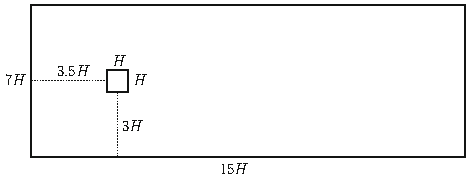
\includegraphics[width=\linewidth]{figures/Appendix_D/Fig_D_16__PDFp779__Bookp774.pdf}
 \captionof{figure}{例题 D.14:$z=0$ 平面上的计算区域底面.}\label{fig:appendix-d-16}
\end{elegantfigure}
\begin{eleganttable}
\captionof{table}{例题 D.14 入口条件的平均速度值.}\label{tab:appendix-d-4}
\begin{tabular}{rrrrrrrr}
\toprule
点 & $u_{1,\mathrm{mean}}$ & 点 & $u_{1,\mathrm{mean}}$ & 点 & $u_{1,\mathrm{mean}}$ & 点 & $u_{1,\mathrm{mean}}$\\
\midrule
0&0&17&1.0315&33&1.0930&49&1.0083\\
1&0.2166&18&1.0461&34&1.0928&50&0.9871\\
2&0.6292&19&1.0587&35&1.0924&51&0.9654\\
3&0.6926&20&1.0661&36&1.0921&52&0.9445\\
4&0.7307&21&1.0723&37&1.0911&53&0.9229\\
5&0.7671&22&1.0770&38&1.0898&54&0.9029\\
6&0.7941&23&1.0813&39&1.0885&55&0.8814\\
7&0.8191&24&1.0843&40&1.0869&56&0.8622\\
8&0.8466&25&1.0868&41&1.0835&57&0.8360\\
9&0.8716&26&1.0890&42&1.0796&58&0.8091\\
10&0.8931&27&1.0890&43&1.0747&59&0.7851\\
11&0.9168&28&1.0890&44&1.0679&60&0.7582\\
12&0.9367&29&1.0890&45&1.0606&61&0.7199\\
13&0.9586&30&1.0900&46&1.0527&62&0.6857\\
14&0.9787&31&1.0930&47&1.0388&63&0.4141\\
15&0.9986&32&1.0930&48&1.0222&64&0\\
16&1.0153&&&&&&\\
\bottomrule
\end{tabular}
\par\smallskip
\parbox{0.95\linewidth}{\centering 入口 65 个等距节点上的平均值,据 J. Hoffman 提供的个人通信.点 0 对应 $z=0$,点 64 对应 $z=2H$.}
\end{eleganttable}

立方体、通道底面和顶面均施加无滑移条件;侧向边界施加自由滑移条件\hyperref[eq:free-slip-condition]{(2.34)};出口可采用 do-nothing 条件\hyperref[eq:do-nothing-condition]{(2.37)}.初始条件未知.可将初始时刻的入口速度插值到区域内部,同时在所有施加无滑移条件的边界上取零,再继续模拟,直至流场充分发展.\textcite{Hoffman2005,HoffmanJohnson2006} 的结果表明,这一状态约在 $3$ 至 $5$ 秒后达到.

入口平均速度约为 $1\,\mathrm{m/s}$.取 Reynolds 数的特征尺度 $U=1\,\mathrm{m/s}$、$H=0.1\,\mathrm m$,并令运动黏度为 $\nu=2.5\times10^{-6}\,\mathrm{m^2/s}$,得到 $\mathrm{Re}=40000$,流动为湍流.再取特征长度 $L=1\,\mathrm m$ 和速度 $U=1\,\mathrm{m/s}$ 推导无量纲 Navier--Stokes 方程\hyperref[eq:time-dependent-ns-strong]{(7.1)},其中无量纲黏度为 $\nu=1/400000$.图\hyperref[fig:appendix-d-17]{D.17}展示了一个流场快照.
\begin{elegantfigure}[0.92\linewidth]
 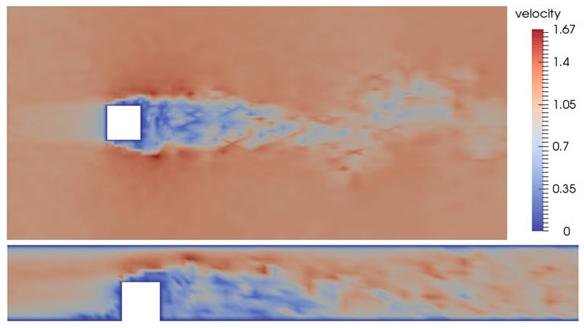
\includegraphics[width=\linewidth]{figures/Appendix_D/Fig_D_17__PDFp780__Bookp775.pdf}
 \captionof{figure}{例题 D.14:$z=H$(上)和 $y=3.5H$(下)截面中的速度模快照.}\label{fig:appendix-d-17}
\end{elegantfigure}

\textcite{Hoffman2005,HoffmanJohnson2006} 的数值研究重点是立方体所受的平均阻力系数.研究使用自适应加密网格和 SUPG 稳定化;具体而言,在式\hyperref[eq:oseen-spg-bilinear-form]{(5.34)}残量中加入 $\partial_t\bm u$,从而形成所谓隐式 LES 模型.网格加密由 DWR 方法控制,见第\hyperref[sec:steady-ns-dwr]{6.4}节.对 $4$ 秒区间作时间平均后,得到平均阻力系数 $\overline c_{\mathrm{drag}}\approx1.5$.流动呈统计周期性,故 $\overline c_{\mathrm{lift}}=0$.计算阻力和升力系数可使用公式\hyperref[eq:appendix-d-5]{(D.5)}和\hyperref[eq:appendix-d-8]{(D.8)}.此例取 $L=1\,\mathrm m$、$V=U$、$A=H^2$,并令 $\bm w_{\mathrm{drag}}=(1,0,0)^\mathsf T$、$\bm w_{\mathrm{lift}}=(0,1,0)^\mathsf T$.
由于物体边界与通道边界相连,实际定义 $\bm w_{\mathrm{drag}}$ 和 $\bm w_{\mathrm{lift}}$ 时,需按笔记\hyperref[note:appendix-d-2]{D.2}作相应修改,例如采用例题\hyperref[ex:appendix-d-6]{D.6}介绍的处理方式.
\end{example}

\backmatter
% Retain the source bibliography's 2006a/2006b entries so the cited 2006c
% work keeps its original year suffix.
\nocite{Gravemeier2006a,Gravemeier2006b}
\printbibliography[heading=bibintoc,title={参考文献}]
\printindex
\end{document}
